\documentclass[10pt,twocolumn,letterpaper]{pfbook} % book class customized for perfbook
% For arxiv.org, must be on or before line 5:
\pdfoutput=1

% To accomodate change in Ghostscript 9.26 (default output: PDF 1.7)
\pdfminorversion=7

% Suppress warning emitted when multiple figures drawn by inkscape appear
% within a page. See: https://tex.stackexchange.com/questions/183149/
\ifdefined\pdfsuppresswarningpagegroup \pdfsuppresswarningpagegroup=1 \fi

% standard packages

% A more pleasant font
\usepackage{lmodern}
\usepackage[T1]{fontenc} % use postscript type 1 fonts
\usepackage[defaultsups]{newtxtext} % use nice, standard fonts for roman
\usepackage{textcomp} % use symbols in TS1 encoding

% Improves the text layout
\usepackage{microtype}
\UseMicrotypeSet[protrusion]{basicmath} % disable protrusion for tt fonts
\usepackage{etoolbox}

\usepackage{fixltx2e} % for \textsubscript, nop on Tex Live 2015 and later
\usepackage{float}
\floatstyle{ruled}
\newfloat{listing}{tbhp}{lst}[chapter]
\floatname{listing}{Listing}
\usepackage{lscape}
\usepackage{epsfig}
\usepackage{subfig}
\newsubfloat{listing}
\captionsetup{labelfont=bf}
\captionsetup[listing]{font=small,labelsep=colon}
\captionsetup[subfloat]{font=small}
% \usepackage{breakurl}
\usepackage{graphicx}
\usepackage{rotating}
\usepackage{setspace}
\usepackage[shortlabels]{enumitem}
\setlist[description]{style=unboxed}
\newlist{sequence}{enumerate}{10}
\setlist[sequence]{label*=\arabic*}
%\usepackage{enumerate}
\usepackage{ifthen}
\usepackage[table,svgnames]{xcolor}
\usepackage[shortcuts]{extdash}
\usepackage{changepage}
\usepackage{listings}
\lstset{basicstyle=\ttfamily}
% \usepackage[strings]{underscore}
% \usepackage{underscore}
\usepackage{pifont} % symbols for qqz reference points and carriagereturn
\usepackage{gensymb} % symbols for both text and math modes such as \degree and \micro
\usepackage{verbatimbox}[2014/01/30] % for centering verbatim listing in figure environment
\usepackage{fancyvrb}
\usepackage{fvextra}[2016/09/02]
\usepackage[bottom]{footmisc} % place footnotes under floating figures/tables
\usepackage{tabularx}
\usepackage[hyphens]{url}
\usepackage{threeparttable}
\usepackage{titlesec}[2016/03/21] % Suppress number in paragraph heading
\usepackage{fmtcount}
\usepackage{draftwatermark}[2015/02/19]
\SetWatermarkAngle{0.0}
\SetWatermarkFontSize{8pt}
\SetWatermarkScale{1.0}
\SetWatermarkLightness{.6}
\SetWatermarkHorCenter{.85\paperwidth}
\SetWatermarkVerCenter{.95\paperheight}
\SetWatermarkText{\texttt{\commitid}}
\usepackage[breakable,skins]{tcolorbox}
\usepackage[split,makeindex]{splitidx}
\usepackage[nottoc]{tocbibind}
\usepackage[columns=3,totoc,indentunit=12pt,justific=raggedright,font=small,columnsep=.15in,unbalanced]{idxlayout}
\usepackage{placeins}
\usepackage[bookmarks=true,bookmarksnumbered=true,pdfborder={0 0 0},linktoc=all]{hyperref}
\usepackage{footnotebackref} % to enable cross-ref of footnote
\usepackage[all]{hypcap} % for going to the top of figure and table
\usepackage{epigraph}[2020/01/02] % latest version prevents orphaned epigraph
\setlength{\epigraphwidth}{2.6in}
\usepackage[xspace]{ellipsis}
\usepackage{braket} % for \ket{} macro in QC section
\usepackage{siunitx} % for \num{} macro
\sisetup{group-minimum-digits=4,group-separator={,},group-digits=integer}
\usepackage{multirow}
\usepackage{noindentafter}
\NoIndentAfterCmd{\epigraph}
\usepackage[all]{nowidow}
\titleformat{\paragraph}[runin]{\normalfont\normalsize\bfseries}{}{0pt}{}

% custom packages
\newboolean{qqzbg}
\setboolean{qqzbg}{false} % overriden by target specific setting
\newcommand{\IfQqzBg}[2]{\ifthenelse{\boolean{qqzbg}}{#1}{#2}}
\newboolean{noqqz}
\setboolean{noqqz}{false}
\newcommand{\IfNoQqz}[2]{\ifthenelse{\boolean{noqqz}}{#1}{#2}}
\newboolean{qqzchpend}
\setboolean{qqzchpend}{false}
\newcommand{\IfQqzChpEnd}[2]{\ifthenelse{\boolean{qqzchpend}}{#1}{#2}}

\input{autodate} % need to input here to reflect tag state
\usepackage{qqz}
\usepackage{origpub}

% custom booleans

\newboolean{inbook}
\setboolean{inbook}{true}
\newcommand{\IfInBook}[2]{\ifthenelse{\boolean{inbook}}{#1}{#2}}
\newboolean{twocolumn}
\setboolean{twocolumn}{true}
\newcommand{\IfTwoColumn}[2]{\ifthenelse{\boolean{twocolumn}}{#1}{#2}}
\newboolean{hardcover}
\setboolean{hardcover}{false}
\newcommand{\IfHardCover}[2]{\ifthenelse{\boolean{hardcover}}{#1}{#2}}
\newboolean{afourpaper}
\setboolean{afourpaper}{false}
\newcommand{\IfAfourPaper}[2]{\ifthenelse{\boolean{afourpaper}}{#1}{#2}}
\newboolean{sansserif}
\setboolean{sansserif}{false}
\newcommand{\IfSansSerif}[2]{\ifthenelse{\boolean{sansserif}}{#1}{#2}}
\newboolean{lmttforcode}
\setboolean{lmttforcode}{true}
\newcommand{\IfLmttForCode}[2]{\ifthenelse{\boolean{lmttforcode}}{#1}{#2}}
\newboolean{tblcptop}
\setboolean{tblcptop}{true}
\newcommand{\IfTblCpTop}[2]{\ifthenelse{\boolean{tblcptop}}{#1}{#2}}
\newboolean{nimbusavail}
\setboolean{nimbusavail}{false}
\newcommand{\IfNimbusAvail}[2]{\ifthenelse{\boolean{nimbusavail}}{#1}{#2}}
\newboolean{colorlinks}
\setboolean{colorlinks}{false}
\newcommand{\IfColorLinks}[2]{\ifthenelse{\boolean{colorlinks}}{#1}{#2}}
\newboolean{toarxiv}
\setboolean{toarxiv}{false}
\newcommand{\IfToArxiv}[2]{\ifthenelse{\boolean{toarxiv}}{#1}{#2}}
\newboolean{indexon}
\setboolean{indexon}{false}
\newcommand{\IfIndexOn}[2]{\ifthenelse{\boolean{indexon}}{#1}{#2}}
\newboolean{indexhl}
\setboolean{indexhl}{false}
\newcommand{\IfIndexHl}[2]{\ifthenelse{\boolean{indexhl}}{#1}{#2}}

% Custom commands for index
\newindex[API Index]{api} % index for API
\newindex[People Name Index]{ppl} % index for People Name
\newcommand{\categapi}[1]{~{\scriptsize (#1)}}
\IfIndexHl{
\newcommand{\hlindex}[1]{\textcolor{DarkGreen}{#1}}
}{
\newcommand{\hlindex}[1]{#1}
}
\newcommand{\IX}[1]{\hlindex{#1}\index{#1}} % put as is into general index
\newcommand{\IXalt}[2]{\hlindex{#1}\index{#2}} % put alternative into general index
\newcommand{\apic}[1]{\hlindex{\co{#1}}\sindex[api]{#1@\co{#1}\categapi{c}}}
\newcommand{\apig}[1]{\hlindex{\co{#1}}\sindex[api]{#1@\co{#1}\categapi{g}}}
\newcommand{\apipx}[1]{\hlindex{\co{#1}}\sindex[api]{#1@\co{#1}\categapi{px}}}
\newcommand{\apik}[1]{\hlindex{\co{#1}}\sindex[api]{#1@\co{#1}\categapi{k}}}
\newcommand{\apikh}[1]{\hlindex{\co{#1}}\sindex[api]{#1@\co{#1}\categapi{k historic}}}
\newcommand{\apipf}[1]{\hlindex{\co{#1}}\sindex[api]{#1@\co{#1}\categapi{pf}}}
\newcommand{\apiur}[1]{\hlindex{\co{#1}}\sindex[api]{#1@\co{#1}\categapi{userspace RCU}}}
\newcommand{\api}[1]{\hlindex{\co{#1}}\sindex[api]{#1@\co{#1}}}
\newcommand{\apialtc}[2]{\hlindex{\co{#1}}\sindex[api]{#2@\co{#2}\categapi{c}}}
\newcommand{\apialtg}[2]{\hlindex{\co{#1}}\sindex[api]{#2@\co{#2}\categapi{g}}}
\newcommand{\apialtk}[2]{\hlindex{\co{#1}}\sindex[api]{#2@\co{#2}\categapi{k}}}
\newcommand{\ppl}[2]{\hlindex{#1 #2}\index{#2, #1}} % forename surname in text, "surname, forename" into ppl index
\newcommand{\pplmdl}[2]{\hlindex{#1~#2}\index{#2, #1}} % for abbreviated middle name
\newcommand{\pplsur}[2]{\hlindex{#2}\index{#2, #1}} % surname in text, "surname, givenname" into ppl index
\newcommand{\pplalt}[2]{\hlindex{#1}\index{#2}} % put 1st arg in text, put 2nd arg into ppl index

\IfTwoColumn{}{
  \setboolean{colorlinks}{true}
  \renewcommand\footnotelayout{%
    \advance\leftskip 0.0in
    \advance\rightskip 0.7in
  }
}

\IfColorLinks{
\hypersetup{colorlinks=true,allcolors=MediumBlue}
}{}

\IfToArxiv{
\hypersetup{
    colorlinks=true,
    linkcolor=black,
    citecolor=black,
    filecolor=black,
    urlcolor=black,
}
}{}

\IfNimbusAvail{
\usepackage{nimbusmononarrow}
}{}
\renewcommand*\ttdefault{lmtt}
%msfontstub

\newcommand{\OneColumnHSpace}[1]{\IfTwoColumn{}{\hspace*{#1}}}

\IfSansSerif{
\renewcommand{\familydefault}{\sfdefault}
\normalfont
\usepackage[slantedGreek,scaled=.96]{newtxsf}
}{
\usepackage[slantedGreek]{newtxmath} % math package to be used with newtxtext
% Poor person's slanted shape for roman --- newtxtext lacks slanted shape
\AtBeginDocument{%
  \DeclareFontShape{\encodingdefault}{\rmdefault}{m}{sl}{<-> ptmro7t}{}%
  \DeclareFontShape{\encodingdefault}{\rmdefault}{b}{sl}{<-> ptmbo7t}{}%
  \DeclareFontShape{\encodingdefault}{\rmdefault}{bx}{sl}{<->ssub * ptm/b/sl}{}%
}
}

\newcommand{\LstLineNo}{\makebox[5ex][r]{\arabic{VerbboxLineNo}\hspace{2ex}}}

\usepackage{bm} % for bold math mode fonts --- should be after math mode font choice
\usepackage{booktabs}
\usepackage{arydshln}
\definecolor{lightgray}{gray}{0.9} % for coloring alternate rows in table

\fvset{fontsize=\scriptsize,obeytabs=true}
\IfTwoColumn{
\fvset{tabsize=2}
}{
\fvset{tabsize=8}
}
\DefineVerbatimEnvironment{VerbatimL}{Verbatim}%
{numbers=left,numbersep=5pt,xleftmargin=9pt}
\AfterEndEnvironment{VerbatimL}{\vspace*{-9pt}}
\DefineVerbatimEnvironment{VerbatimN}{Verbatim}%
{numbers=left,numbersep=3pt,xleftmargin=5pt,xrightmargin=5pt,frame=single}
\DefineVerbatimEnvironment{VerbatimU}{Verbatim}%
{numbers=none,xleftmargin=5pt,xrightmargin=5pt,samepage=true,frame=single}

\IfLmttForCode{
\AtBeginEnvironment{verbatim}{\renewcommand{\ttdefault}{lmtt}}
\AtBeginEnvironment{verbbox}{\renewcommand{\ttdefault}{lmtt}}
\AtBeginEnvironment{table}{\renewcommand{\ttdefault}{lmtt}}
\AtBeginEnvironment{table*}{\renewcommand{\ttdefault}{lmtt}}
\AtBeginEnvironment{sidewaystable*}{\renewcommand{\ttdefault}{lmtt}}
\AtBeginEnvironment{minipage}{\renewcommand{\ttdefault}{lmtt}}
\AtBeginEnvironment{listing}{\renewcommand{\ttdefault}{lmtt}}
\AtBeginEnvironment{listing*}{\renewcommand{\ttdefault}{lmtt}}
\fvset{fontfamily=lmtt}
}{}

\IfTblCpTop{
\floatstyle{plaintop}
\restylefloat{table}
\addtolength{\abovecaptionskip}{-2.5pt}
\setlength{\abovetopsep}{-2pt}
}{}
\captionsetup{hangindent=20pt}
\captionsetup[listing]{hangindent=20pt}

\usepackage[capitalise,noabbrev,nosort]{cleveref}
\crefname{subsubsubappendix}{Appendix}{Appendices}
\crefname{sublisting}{Listing}{Listings}
\crefname{sequencei}{step}{steps}
\Crefname{sequencei}{Step}{Steps}
\crefname{page}{page}{pages}
\Crefname{page}{Page}{Pages}
\newcommand{\crefrangeconjunction}{--}
\newcommand{\creflastconjunction}{, and~}

% Define \crefthro{} for "Sections~m.n through~m.p"
\newcommand{\crefthro}[2]{%
  \namecrefs{#1}~\ref{#1} through~\ref{#2}%
}
\newcommand{\Crefthro}[2]{%
  \nameCrefs{#1}~\ref{#1} through~\ref{#2}%
}

% Define \clnref{} and \Clnref{} for reference to line labels
\newcounter{lblcount}
\newcommand{\clnrefp}[2]{%
  \setcounter{lblcount}{0}% Restart label count
  \renewcommand*{\do}[1]{\stepcounter{lblcount}}% Count label
  \docsvlist{#1}% Process list and count labels
  \def\nextitem{\def\nextitem{, }}% Separator
  \ifnum\value{lblcount}=1 #2~\lnref{#1}%
  \else\ifnum\value{lblcount}=2 {#2}s~%
  \renewcommand*{\do}[1]{%
    \addtocounter{lblcount}{-1}%
    \ifnum\value{lblcount}=0 { }and~\else\nextitem\fi\lnref{##1}}% How to process each label
  \else {#2}s~%
  \renewcommand*{\do}[1]{%
    \addtocounter{lblcount}{-1}%
    \ifnum\value{lblcount}=0 , and~\else\nextitem\fi\lnref{##1}}% How to process each label
  \fi%
  \docsvlist{#1}% Process list
  \fi%
}
\newcommand{\clnref}[1]{\clnrefp{#1}{line}}
\newcommand{\Clnref}[1]{\clnrefp{#1}{Line}}
\newcommand{\clnrefrange}[2]{lines~\lnref{#1}\==\lnref{#2}}
\newcommand{\Clnrefrange}[2]{Lines~\lnref{#1}\==\lnref{#2}}
\newcommand{\clnrefthro}[2]{lines~\lnref{#1} through~\lnref{#2}}
\newcommand{\Clnrefthro}[2]{Lines~\lnref{#1} through~\lnref{#2}}
\newcommand{\pararef}[1]{Paragraph ``\nameref{#1}'' on Page~\pageref{#1}}
\newcommand{\Pararef}[1]{Paragraph ``\nameref{#1}'' on Page~\pageref{#1}}

% geometry setting
\newlength{\twocolumnwidth}
\newlength{\onecolumntextwidth}
\setlength{\onecolumntextwidth}{4.75in}
\IfTwoColumn{
  \setlength{\twocolumnwidth}{\columnwidth}
  \renewcommand\floatpagefraction{.75}
  \IfHardCover{
    \usepackage[papersize={8.25in,10.75in},body={6.5in,8.25in},twocolumn,columnsep=0.25in]{geometry}
  }{
    \IfAfourPaper{
      \usepackage[a4paper,body={6.5in,8.25in},twocolumn,columnsep=0.25in]{geometry}
    }{
      \usepackage[letterpaper,body={6.5in,8.25in},twocolumn,columnsep=0.25in]{geometry}      
}}}{ % One Column
  \setlength{\twocolumnwidth}{3.125in}
  \IfHardCover{
    \usepackage[papersize={8.25in,10.75in},body={4.75in,8.25in},onecolumn]{geometry}
  }{
    \IfAfourPaper{
    \usepackage[a4paper,body={4.75in,8.25in},onecolumn]{geometry}
    }{
    \usepackage[letterpaper,body={4.75in,8.25in},onecolumn]{geometry}
  }}
  \geometry{hcentering=true} % horizontal centering for 1c layouts
}
\IfAfourPaper{
  \geometry{vcentering=true} % vertical centering for A4 paper
}{
  \geometry{vmarginratio=3:4}
}

\setcounter{topnumber}{3}
\renewcommand\topfraction{.75}
\setcounter{bottomnumber}{2}
\renewcommand\bottomfraction{.3}
\setcounter{totalnumber}{5}
\renewcommand\textfraction{.15}
\renewcommand\floatpagefraction{.6}
\setcounter{dbltopnumber}{3}
\renewcommand\dbltopfraction{.75}
\renewcommand\dblfloatpagefraction{.5}

\IfAfourPaper{
\SetWatermarkVerCenter{.92\paperheight}
}{}

\IfHardCover{
\SetWatermarkVerCenter{.95\paperheight}
}{}

\begin{document}

%%HTMLSKIP
\lstset{
 literate={\_}{}{0\discretionary{\_}{}{\_}}%
  {\_\_}{}{0\discretionary{\_\_}{}{\_\_}}%
  {->}{}{0\discretionary{->}{}{->}}%
}
%%HTMLNOSKIP
\newcommand{\co}[1]{\lstinline[breaklines=true,breakatwhitespace=true]{#1}}
\newcommand{\nbco}[1]{\hbox{\lstinline[breaklines=false,breakatwhitespace=false]{#1}}} % no break lines for short snippet
\newcommand{\qco}[1]{``\nbco{#1}''} % \nbco with quotation marks
\newcommand{\tco}[1]{\texttt{\detokenize{#1}}} % for code in tabular environment
% \tco{} will break at spaces but not at underscores
\newcommand{\qtco}[1]{``\hbox{\tco{#1}}''} % \tco with quotation marks
\newcommand{\lopt}[1]{\tco{-}\tco{-}\tco{#1}} % to avoid "--" to endash conversion
\newcommand{\nf}[1]{\textnormal{#1}} % to return to normal font
\newcommand{\qop}[1]{{\sffamily #1}} % QC operator such as H, T, S, etc.

\DeclareRobustCommand{\euler}{\ensuremath{\mathrm{e}}}
\DeclareRobustCommand{\O}[1]{\ensuremath{\mathcal{O}\left(#1\right)}}
\DeclareRobustCommand{\Node}[1]{Node~{\ensuremath{#1}}}
\newcommand{\Power}[1]{POWER#1}
\newcommand{\ARM}[1]{Arm{#1}}
\newcommand{\ARMv}[1]{Armv{#1}}
\newcommand{\GNUC}{GNU~C}
\newcommand{\GCC}{GCC}
%\newcommand{\GCC}{\co{gcc}} % For those who prefer "gcc"
\newcommand{\IRQ}{IRQ}
%\newcommand{\IRQ}{irq}      % For those who prefer "irq"
\newcommand{\rt}{\mbox{-rt}} % to prevent line break behind "-"

\newcommand{\Epigraph}[2]{\epigraphhead[65]{\epigraph{#1}{#2}}}

% Hyphenation exceptions for US English,
% based on hyphenation exception log articles in TUGboat.
%
% Copyright 2008 TeX Users Group.
% You may freely use, modify and/or distribute this file.
%
% This is an automatically generated file.  Do not edit!
%
% Please contact the TUGboat editorial staff <tugboat@tug.org>
% for corrections and omissions.

\hyphenation{
  acad-e-my
  acad-e-mies
  ac-cu-sa-tive
  acro-nym
  acro-nyms
  acryl-amide
  acryl-amides
  acryl-alde-hyde
  acu-punc-ture
  acu-punc-tur-ist
  add-a-ble
  add-i-ble
  adren-a-line
  aero-space
  af-ter-thought
  af-ter-thoughts
  agron-o-mist
  agron-o-mists
  al-ge-bra-i-cal-ly
  am-phet-a-mine
  am-phet-a-mines
  anach-ro-nism
  anach-ro-nis-tic
  an-a-lyse
  an-a-lysed
  analy-ses
  analy-sis
  an-eu-rysm
  an-eu-rysms
  an-eu-rys-mal
  an-iso-trop-ic
  an-iso-trop-i-cal-ly
  an-isot-ro-pism
  an-isot-ropy
  an-ni-ver-sary
  an-ni-ver-saries
  anom-a-ly
  anom-a-lies
  anti-deriv-a-tive
  anti-deriv-a-tives
  anti-holo-mor-phic
  an-tin-o-my
  an-tin-o-mies
  anti-nu-clear
  anti-nu-cle-on
  anti-rev-o-lu-tion-ary
  a-peri-odic
  apoth-e-o-ses
  apoth-e-o-sis
  ap-pen-di-ces
  ap-pen-dix
  ap-pen-dixes
  ar-chi-me-dean
  ar-chi-pel-ago
  ar-chi-pel-a-gos
  ar-chive
  ar-chives
  ar-chiv-ing
  ar-chiv-ist
  ar-chiv-ists
  ar-che-typ-al
  ar-che-type
  ar-che-types
  ar-che-typ-i-cal
  arc-tan-gent
  arc-tan-gents
  a-spher-ic
  a-spher-i-cal
  as-sign-a-ble
  as-sign-or
  as-sign-ors
  as-sist-ant
  as-sist-ance
  as-sist-ant-ship
  as-sist-ant-ships
  as-trol-o-ger
  as-trol-o-gers
  as-tron-o-mer
  as-tron-o-mers
  asymp-to-matic
  as-ymp-tot-ic
  asyn-chro-nous
  ath-er-o-scle-ro-sis
  at-mos-phere
  at-mos-pheres
  at-tri-bute
  at-trib-uted
  at-trib-ut-able
  au-to-ma-tion
  au-tom-a-ton
  au-tom-a-ta
  auto-num-ber-ing
  au-ton-o-mous
  auto-re-gres-sion
  auto-re-gres-sive
  auto-round-ing
  av-oir-du-pois
  back-scratcher
  back-scratch-ing
  band-lead-er
  band-lead-ers
  bank-rupt
  bank-rupts
  bank-rupt-cy
  bank-rupt-cies
  bar-onies
  base-line-skip
  ba-thym-e-try
  bathy-scaphe
  bean-ies
  be-drag-gle
  be-drag-gled
  bed-rid-den
  bed-rock
  be-dwarf
  be-dwarfs
  be-hav-iour
  be-hav-iours
  bevies
  bib-lio-graph-i-cal
  bib-li-og-ra-phy-style
  bib-units
  bi-dif-fer-en-tial
  big-gest
  big-shot
  big-shots
  bill-able
  bio-math-e-mat-ics
  bio-med-i-cal
  bio-med-i-cine
  bio-rhythms
  bio-weap-ons
  bio-weap-on-ry
  bit-map
  bit-maps
  bland-er
  bland-est
  blind-er
  blind-est
  blondes
  blue-print
  blue-prints
  bo-lom-e-ter
  bo-lom-e-ters
  book-sell-er
  book-sell-ers
  bool-ean
  bool-eans
  bor-no-log-i-cal
  bot-u-lism
  brusquer
  buf-fer
  buf-fers
  bun-gee
  bun-gees
  busier
  busi-est
  bussing
  butted
  buzz-word
  buzz-words
  cache-abil-ity
  cache-able
  ca-coph-o-ny
  ca-coph-o-nies
  call-er
  call-ers
  cam-era-men
  cart-wheel
  cart-wheels
  ca-tarrh
  ca-tarrhs
  ca-tas-tro-phe
  ca-tas-tro-phes
  cat-a-stroph-ic
  cat-a-stroph-i-cally
  ca-tas-tro-phism
  cat-e-noid
  cat-e-noids
  cau-li-flow-er
  chan-cery
  chap-ar-ral
  char-treuse
  chemo-kine
  chemo-kines
  chemo-ther-apy
  chemo-ther-a-pies
  chloro-meth-ane
  chloro-meth-anes
  cho-les-teric
  cig-a-rette
  cig-a-rettes
  cinque-foil
  co-asso-cia-tive
  coch-leas
  coch-lear
  co-designer
  co-designers
  co-gnac
  co-gnacs
  co-ker-nel
  co-ker-nels
  col-lin-ea-tion
  col-umns
  com-par-and
  com-par-ands
  com-pen-dium
  com-po-nent-wise
  comp-trol-ler
  comp-trol-lers
  com-put-able
  com-put-abil-ity
  con-form-able
  con-form-ist
  con-form-ists
  con-form-ity
  con-ge-ries
  con-gress
  con-gresses
  con-struc-ted
  con-struc-ti-ble
  con-struc-ti-bil-ity
  con-trib-ute
  con-trib-utes
  con-trib-uted
  copy-right-able
  co-re-la-tion
  co-re-la-tions
  co-re-li-gion-ist
  co-re-li-gion-ists
  co-re-op-sis
  co-re-spon-dent
  co-re-spon-dents
  co-se-cant
  co-semi-sim-ple
  co-tan-gent
  cour-ses
  co-work-er
  co-work-ers
  crank-case
  crank-shaft
  croc-o-dile
  croc-o-diles
  cross-hatch
  cross-hatched
  cross-hatch-ing
  cross-over
  cryp-to-gram
  cryp-to-grams
  cuff-link
  cuff-links
  cu-nei-form
  cus-tom-iz-a-ble
  cus-tom-ize
  cus-tom-izes
  cus-tom-ized
  cy-ber-virus
  cy-ber-viruses
  cy-ber-wea-pon
  cy-ber-wea-pons
  cy-to-kine
  cy-to-kines
  dachs-hund
  dam-sel-fly
  dam-sel-flies
  dactyl-o-gram
  dactyl-o-graph
  data-base
  data-bases
  data-path
  data-paths
  date-stamp
  date-stamps
  de-allo-cate
  de-allo-cates
  de-allo-cated
  de-allo-ca-tion
  de-allo-ca-tions
  de-clar-able
  de-fin-i-tive
  de-lec-ta-ble
  demi-semi-qua-ver
  demi-semi-qua-vers
  de-moc-ra-tism
  demos
  der-i-va-tion
  der-i-va-tions
  der-i-va-tion-al
  de-riv-a-tive
  de-riv-a-tives
  dia-lec-tic
  dia-lec-tics
  dia-lec-ti-cian
  dia-lec-ti-cians
  di-chloro-meth-ane
  dif-fract
  dif-fracts
  dif-frac-tion
  dif-frac-tions
  direr
  dire-ness
  dis-par-and
  dis-par-ands
  dis-traught-ly
  dis-trib-ut-able
  dis-trib-ute
  dis-trib-utes
  dis-trib-uted
  dis-trib-u-tive
  dou-ble-space
  dou-ble-spaced
  dou-ble-spac-ing
  dou-ble-talk
  doll-ish
  drift-age
  driv-ers
  drom-e-dary
  drom-e-daries
  drop-let
  drop-lets
  du-op-o-list
  du-op-o-lists
  du-op-o-ly
  du-op-o-lies
  dys-lexia
  dys-lec-tic
  dys-topia
  east-end-ers
  eco-sys-tem
  eco-sys-tems
  eco-nom-ics
  econ-o-mies
  econ-o-mist
  econ-o-mists
  ei-gen-class
  ei-gen-classes
  ei-gen-val-ue
  ei-gen-val-ues
  electro-mechan-i-cal
  electro-mechano-acoustic
  elec-tro-pho-re-sis
  elec-tro-pho-ret-ic
  elit-ist
  elit-ists
  en-dos-copy
  en-dos-copies
  en-tre-pre-neur
  en-tre-pre-neurs
  en-tre-pre-neur-ial
  ep-i-neph-rine
  eps-to-pdf
  equi-vari-ant
  equi-vari-ance
  er-go-nom-ic
  er-go-nom-ics
  er-go-nom-i-cally
  es-sence
  es-sences
  eth-ane
  eth-yl-am-ine
  eth-yl-ate
  eth-yl-ated
  eth-yl-ene
  ethy-nyl
  ethy-nyl-a-tion
  eu-sta-chian
  ever-si-ble
  evert
  everts
  evert-ed
  evert-ing
  ex-plan-a-tory
  ex-quis-ite
  ex-tra-or-di-nary
  face-lifts
  face-lift-ing
  fall-ing
  fermi-ons
  figu-rine
  figu-rines
  fi-nite-ly
  fla-gel-lum
  fla-gel-la
  flam-ma-bles
  fledg-ling
  flow-chart
  flow-charts
  fluoro-car-bon
  fluor-os-copies
  fluor-os-copy
  for-mi-da-ble
  for-mi-da-bly
  for-syth-ia
  forth-right
  free-loader
  free-loaders
  friend-lier
  friend-li-est
  fri-vol-ity
  fri-vol-i-ties
  friv-o-lous
  front-end
  front-ends
  ga-lac-tic
  gal-axy
  gal-ax-ies
  gaz-et-teer
  gaz-et-teers
  gas-om-e-ter
  ge-o-des-ic
  ge-o-det-ic
  ge-om-eter
  ge-om-eters
  geo-met-ric
  geo-met-rics
  ge-o-strophic
  geo-ther-mal
  ge-ot-ro-pism
  giga-nodes
  gno-mon
  gno-mons
  gran-di-ose
  grand-uncle
  grand-uncles
  griev-ance
  griev-ances
  griev-ous
  griev-ous-ly
  group-like
  hair-style
  hair-styles
  hair-styl-ist
  hair-styl-ists
  half-life
  half-lives
  half-space
  half-spaces
  half-tone
  half-tones
  half-way
  har-bin-ger
  har-bin-gers
  har-le-quin
  har-le-quins
  hatch-eries
  hei-nous
  he-lio-pause
  he-lio-trope
  hemi-demi-semi-qua-ver
  hemi-demi-semi-qua-vers
  he-mo-glo-bin
  he-mo-phil-ia
  he-mo-phil-iac
  he-mo-phil-iacs
  hemo-rhe-ol-ogy
  he-pat-ic
  he-pat-ica
  her-maph-ro-dite
  her-maph-ro-dit-ic
  he-roes
  hexa-dec-i-mal
  hip-po-po-ta-mus
  holo-deck
  holo-decks
  ho-lo-no-my
  ho-meo-mor-phic
  ho-meo-mor-phism
  ho-meo-stat-ic
  ho-meo-stat-ics
  ho-meo-sta-sis
  ho-mo-thetic
  horse-rad-ish
  hot-bed
  hot-beds
  hounds-teeth
  hounds-tooth
  hy-dro-ther-mal
  hy-per-elas-tic-ity
  hy-phen-a-tion
  hy-phen-a-tions
  hy-po-elas-tic-ity
  hy-po-thal-a-mus
  ico-nog-ra-pher
  ico-nog-ra-phers
  icon-o-graph-ic
  ico-nog-ra-phy
  ideals
  ideo-graphs
  idio-syn-crasy
  idio-syn-cra-sies
  idio-syn-cratic
  idio-syn-crat-i-cal-ly
  ig-nit-er
  ig-nit-ers
  ig-ni-tor
  ignore-spaces
  il-li-quid
  il-li-quid-ity
  im-mu-ni-za-tion
  im-mu-no-mod-u-la-to-ry
  im-ped-ance
  im-ped-ances
  in-du-bi-ta-ble
  in-fin-ite-ly
  in-fin-i-tes-i-mal
  in-fra-struc-ture
  in-fra-struc-tures
  input-enc
  in-stall-er
  in-stall-ers
  in-teg-rity
  in-ter-dis-ci-pli-nary
  in-ter-ga-lac-tic
  in-ter-view-ee
  in-ter-view-ees
  in-utile
  in-util-i-ty
  ir-ra-tio-nal
  ir-re-duc-ible
  ir-re-duc-ibly
  ir-rev-o-ca-ble
  iso-geo-met-ric
  iso-geo-met-rics
  iso-ther-mal
  isot-ropy
  iso-trop-ic
  itin-er-ary
  itin-er-ar-ies
  je-re-mi-ads
  key-note
  key-notes
  key-stroke
  key-strokes
  kilo-nodes
  kiln-ing
  lac-i-est
  lam-en-ta-ble
  land-scap-er
  land-scap-ers
  lar-ce-n
  lar-ce-ny
  lar-ce-nies
  lar-ce-nist
  leaf-hop-per
  leaf-hop-pers
  leaf-let
  leaf-lets
  let-ter-spaces
  let-ter-spaced
  let-ter-spac-ing
  leu-ko-cyte
  leu-ko-cytes
  leu-ko-triene
  leu-ko-trienes
  life-span
  life-spans
  life-style
  life-styles
  lift-off
  light-weight
  lim-ou-sines
  line-backer
  line-spacing
  li-on-ess
  li-quid-ity
  lith-o-graphed
  lith-o-graphs
  lo-bot-omy
  lo-bot-om-ize
  loges
  long-est
  look-ahead
  lo-quac-ity
  love-struck
  macro-eco-nomic
  macro-eco-nomics
  macro-econ-omy
  make-in-dex
  mal-a-prop-ism
  mal-a-prop-isms
  man-slaugh-ter
  man-u-script
  man-u-scripts
  mar-gin-al
  math-e-ma-ti-cian
  math-e-ma-ti-cians
  mattes
  med-ic-aid
  medi-ocre
  medi-oc-ri-ties
  mega-fau-na
  mega-fau-nal
  mega-lith
  mega-liths
  mega-nodes
  meta-bol-ic
  me-tab-o-lism
  me-tab-o-lisms
  me-tab-o-lite
  me-tab-o-lites
  meta-form
  meta-forms
  meta-lan-guage
  meta-lan-guages
  meta-phor
  meta-phors
  meta-phor-i-cal
  meta-phor-i-cal-ly
  meta-sta-bil-ity
  meta-stable
  meta-table
  meta-tables
  metem-psy-cho-sis
  meth-am-phet-a-mine
  meth-ane
  meth-od
  meth-yl-am-mo-nium
  meth-yl-ate
  meth-yl-ated
  meth-yl-a-tion
  meth-yl-ene
  me-trop-o-lis
  me-trop-o-lises
  met-ro-pol-i-tan
  met-ro-pol-i-tans
  micro-eco-nomic
  micro-eco-nomics
  micro-econ-omy
  micro-en-ter-prise
  micro-en-ter-prises
  mi-cro-fiche
  mi-cro-fiches
  micro-organ-ism
  micro-organ-isms
  mi-cro-struc-ture
  mid-after-noon
  mill-age
  mil-li-liter
  mimeo-graphed
  mimeo-graphs
  mim-ic-ries
  mine-sweeper
  mine-sweepers
  min-is
  mini-sym-po-sium
  mini-sym-po-sia
  mi-nut-er
  mi-nut-est
  mis-chie-vous-ly
  mi-sers
  mi-sog-a-my
  mne-mon-ic
  mne-mon-ics
  mod-el-ling
  mo-lec-u-lar
  mol-e-cule
  mol-e-cules
  mon-archs
  money-len-der
  money-len-ders
  mono-chrome
  mono-en-er-getic
  mon-oid
  mon-oph-thong
  mon-oph-thongs
  mono-pole
  mono-poles
  mo-nop-oly
  mono-space
  mono-spaced
  mono-spacing
  mono-spline
  mono-splines
  mono-strofic
  mo-not-o-nies
  mo-not-o-nous
  mo-ron-ism
  mos-qui-to
  mos-qui-tos
  mos-qui-toes
  mud-room
  mud-rooms
  mul-ti-fac-eted
  mul-ti-plic-able
  mul-ti-plic-ably
  multi-user
  name-space
  name-spaces
  neo-fields
  neo-nazi
  neo-nazis
  neph-ews
  neph-rite
  neph-ritic
  new-est
  news-let-ter
  news-let-ters
  nil-po-tent
  nitro-meth-ane
  node-list
  node-lists
  no-name
  non-ar-ith-met-ic
  non-emer-gency
  non-equi-vari-ance
  none-the-less
  non-euclid-ean
  non-iso-mor-phic
  non-pseudo-com-pact
  non-smooth
  non-uni-form
  non-uni-form-ly
  non-zero
  nor-ep-i-neph-rine
  not-with-stand-ing
  nu-cleo-tide
  nu-cleo-tides
  nut-crack-er
  nut-crack-ers
  oer-steds
  off-line
  off-load
  off-loads
  off-loaded
  oli-gop-o-list
  oli-gop-o-lists
  oli-gop-oly
  oli-gop-ol-ies
  om-ni-pres-ent
  om-ni-pres-ence
  ono-mat-o-poe-ia
  ono-mat-o-po-et-ic
  op-er-and
  op-er-ands
  orang-utan
  orang-utans
  or-tho-don-tist
  or-tho-don-tists
  or-tho-ker-a-tol-ogy
  ortho-nitro-toluene
  over-view
  over-views
  ox-id-ic
  pad-ding
  page-rank
  pain-less-ly
  pal-ette
  pal-ettes
  pa-rab-ola
  par-a-bol-ic
  pa-rab-o-loid
  par-a-digm
  par-a-digms
  para-chute
  para-chutes
  para-di-methyl-benzene
  para-fluoro-toluene
  para-graph-er
  para-le-gal
  par-al-lel-ism
  para-mag-net-ism
  para-medic
  para-methyl-anisole
  pa-ram-e-tri-za-tion
  pa-ram-e-trize
  para-mil-i-tary
  para-mount
  path-o-gen-ic
  peev-ish
  peev-ish-ness
  pen-al-ty
  pen-al-ties
  pen-ta-gon
  pen-ta-gons
  pe-tro-le-um
  phe-nol-phthalein
  phe-nom-e-non
  phenyl-ala-nine
  phi-lat-e-list
  phi-lat-e-lists
  pho-neme
  pho-nemes
  pho-ne-mic
  phos-phor-ic
  pho-to-graphs
  pho-to-off-set
  phtha-lam-ic
  phthal-ate
  phthi-sis
  pic-a-dor
  pic-a-dors
  pipe-line
  pipe-lines
  pipe-lin-ing
  pi-ra-nhas
  placa-ble
  plant-hop-per
  plant-hop-pers
  pla-teau
  pla-teaus
  pleas-ance
  plug-in
  plug-ins
  pol-ter-geist
  poly-an-dr
  poly-an-dry
  poly-an-drous
  poly-dac-tyl
  poly-dac-tyl-lic
  poly-ene
  poly-eth-yl-ene
  po-lyg-a-mist
  po-lyg-a-mists
  polyg-on-i-za-tion
  po-lyg-y-n
  po-lyg-y-ny
  po-lyg-y-nous
  pol-yp
  pol-yps
  po-lyph-o-n
  po-lyph-o-ny
  po-lyph-o-nous
  poly-phon-ic
  poly-styrene
  pome-gran-ate
  poro-elas-tic
  por-ous
  por-ta-ble
  post-am-ble
  post-am-bles
  post-hu-mous
  post-script
  post-scripts
  pos-tur-al
  pre-am-ble
  pre-am-bles
  pre-dict-able
  pre-fers
  pre-loaded
  pre-par-ing
  pre-print
  pre-prints
  pre-proces-sor
  pre-proces-sors
  pres-ent-ly
  pre-split-ting
  pre-wrap
  pre-wrapped
  priest-esses
  pret-ty-prin-ter
  pret-ty-prin-ting
  pro-ce-dur-al
  process
  pro-cur-ance
  prog-e-nies
  prog-e-ny
  pro-gram-mable
  pro-kary-ote
  pro-kary-otes
  pro-kary-ot-ic
  prom-i-nent
  pro-mis-cu-ous
  prom-is-sory
  prom-ise
  prom-ises
  pro-pel-ler
  pro-pel-lers
  pro-pel-ling
  pro-hib-i-tive
  pro-hib-i-tive-ly
  pro-sciut-to
  pros-ta-glan-din
  pros-ta-glan-dins
  pro-style
  pro-styles
  pro-test-er
  pro-test-ers
  pro-tes-tor
  pro-tes-tors
  pro-to-lan-guage
  pro-to-typ-al
  prov-ince
  prov-inces
  pro-vin-cial
  pro-virus
  pro-viruses
  prow-ess
  pseu-do-dif-fer-en-tial
  pseu-do-fi-nite
  pseu-do-fi-nite-ly
  pseu-do-forces
  pseu-dog-ra-pher
  pseu-do-group
  pseu-do-groups
  pseu-do-nym
  pseu-do-nyms
  pseu-do-word
  pseu-do-words
  psy-che-del-ic
  psychs
  pu-bes-cence
  pur-ges
  quad-ding
  qua-drat-ic
  qua-drat-ics
  quad-ra-ture
  quad-ri-lat-er-al
  quad-ri-lat-er-als
  quad-ri-pleg-ic
  quad-ru-ped
  quad-ru-peds
  quad-ru-pole
  quad-ru-poles
  quaint-er
  quaint-est
  qua-si-equiv-a-lence
  qua-si-equiv-a-lences
  qua-si-equiv-a-lent
  qua-si-hy-po-nor-mal
  qua-si-rad-i-cal
  qua-si-resid-ual
  qua-si-smooth
  qua-si-sta-tion-ary
  qua-si-topos
  qua-si-tri-an-gu-lar
  qua-si-triv-ial
  quin-tes-sence
  quin-tes-sences
  quin-tes-sen-tial
  rab-bit-ry
  ra-di-og-ra-phy
  raff-ish
  raff-ish-ly
  ram-shackle
  rav-en-ous
  re-allo-cate
  re-allo-cates
  re-allo-cated
  re-arrange
  re-arranges
  re-arranged
  re-arrange-ment
  re-arrange-ments
  rec-i-proc-i-ties
  rec-i-proc-i-ty
  rec-tan-gle
  rec-tan-gles
  rec-tan-gu-lar
  re-di-rect
  re-di-rect-ion
  re-duc-ible
  re-echo
  re-edu-cate
  ref-u-gee
  ref-u-gees
  re-imple-ment
  re-imple-ments
  re-imple-mented
  re-imple-men-ta-tion
  ren-ais-sance
  re-phrase
  re-phrases
  re-phrased
  re-po-si-tion
  re-po-si-tions
  re-print
  re-prints
  re-print-ed
  re-stor-able
  retro-fit
  retro-fit-ted
  re-us-able
  re-use
  re-wire
  re-wrap
  re-wrapped
  re-write
  rhi-noc-er-os
  right-eous
  right-eous-ness
  ring-leader
  ring-leaders
  ro-bot
  ro-bots
  ro-botic
  ro-bot-ics
  roof-top
  roof-tops
  round-table
  round-tables
  sales-clerk
  sales-clerks
  sales-woman
  sales-women
  sa-lient
  sal-mo-nel-la
  sal-ta-tion
  sar-sa-par-il-la
  sat-el-lite
  sat-el-lites
  sauer-kraut
  scat-o-log-i-cal
  scene-shift-er
  scene-shift-ing
  sched-ul-ing
  schiz-o-phrenic
  schnau-zer
  school-child
  school-child-ren
  school-teacher
  school-teach-ers
  scru-ti-ny
  scyth-ing
  sell-er
  sell-ers
  sec-re-tar-iat
  sec-re-tar-iats
  sem-a-phore
  sem-a-phores
  se-mes-ter
  semi-def-i-nite
  semi-di-rect
  semi-ho-mo-thet-ic
  semi-ring
  semi-rings
  semi-sim-ple
  semi-skilled
  sem-itic
  ser-geant
  ser-geants
  sero-epi-de-mi-o-log-i-cal
  ser-vo-me-chan-i-cal
  ser-vo-mech-a-nism
  ser-vo-mech-a-nisms
  ses-qui-pe-da-lian
  set-up
  set-ups
  se-vere-ly
  shap-able
  shape-able
  shoe-string
  shoe-strings
  shop-lift-er
  shop-lift-ing
  show-hy-phens
  side-step
  side-steps
  side-swipe
  sign-age
  single-space
  single-spaced
  single-spacing
  sky-scraper
  sky-scrapers
  sln-uni-code
  smoke-stack
  smoke-stacks
  snor-kel-ing
  so-le-noid
  so-le-noids
  solute
  solutes
  sov-er-eign
  sov-er-eigns
  spa-ces
  spe-cious
  spell-er
  spell-ers
  spell-ing
  spe-lunk-er
  spend-thrift
  spher-oid
  spher-oids
  spher-oid-al
  sphin-ges
  spic-i-ly
  spin-or
  spin-ors
  spokes-man
  spokes-per-son
  spokes-per-sons
  spokes-woman
  spokes-women
  sports-cast
  sports-cast-er
  spor-tive-ly
  sports-wear
  sports-writer
  sports-writers
  spright-lier
  squea-mish
  stand-alone
  star-tling
  star-tling-ly
  sta-tis-tics
  stealth-ily
  steeple-chase
  stereo-graph-ic
  sto-chas-tic
  strange-ness
  strap-hanger
  strat-a-gem
  strat-a-gems
  stretch-i-er
  strip-tease
  strong-est
  strong-hold
  stu-pid-er
  stu-pid-est
  sub-dif-fer-en-tial
  sub-ex-pres-sion
  sub-ex-pres-sions
  sub-node
  sub-nodes
  sub-scrib-er
  sub-scrib-ers
  sub-tables
  sum-ma-ble
  super-deri-va-tion
  super-deri-va-tions
  super-ego
  super-egos
  su-prem-a-cist
  su-prem-a-cists
  sur-gery
  sur-ge-ries
  sur-ges
  sur-veil-lance
  swim-ming-ly
  symp-to-matic
  syn-chro-mesh
  syn-chro-nous
  syn-chro-tron
  taff-rail
  take-over
  take-overs
  talk-a-tive
  ta-pes-try
  ta-pes-tries
  tar-pau-lin
  tar-pau-lins
  te-leg-ra-pher
  te-leg-ra-phers
  tele-ki-net-ic
  tele-ki-net-ics
  tele-ro-bot-ics
  tell-er
  tell-ers
  tem-po-rar-ily
  ten-ure
  test-bed
  tera-nodes
  tetra-butyl-ammo-nium
  text-height
  text-length
  text-width
  thal-a-mus
  ther-mo-elas-tic
  time-stamp
  time-stamps
  tool-kit
  tool-kits
  topo-graph-i-cal
  topo-iso-mer-ase
  topo-iso-mer-ases
  toques
  trai-tor-ous
  trans-ceiver
  trans-ceivers
  trans-par-en-cy
  trans-par-en-cies
  trans-gress
  trans-ver-sal
  trans-ver-sals
  trans-ves-tite
  trans-ves-tites
  tra-vers-a-ble
  tra-ver-sal
  tra-ver-sals
  tri-ethyl-amine
  treach-eries
  tribes-man
  trip-let
  trip-lets
  tri-plex
  tri-plex-es
  trou-ba-dour
  tur-key
  tur-keys
  turn-around
  turn-arounds
  typ-al
  un-at-tached
  un-err-ing-ly
  un-friend-ly
  un-friend-li-er
  un-in-stan-ti-at-ed
  vaguer
  vaude-ville
  vic-ars
  vil-lain-ess
  vis-ual
  vis-ual-ly
  vi-vip-a-rous
  voice-print
  vspace
  wad-ding
  wall-flower
  wall-flow-ers
  warm-er
  warm-est
  waste-water
  wave-guide
  wave-guides
  wave-let
  wave-lets
  weap-ons
  weap-on-ry
  web-like
  web-log
  web-logs
  week-night
  week-nights
  weight-lift-er
  weight-lift-ing
  wheel-chair
  wheel-chairs
  which-ever
  white-sided
  white-space
  white-spaces
  wide-spread
  wing-span
  wing-spans
  wing-spread
  witch-craft
  word-spac-ing
  work-around
  work-arounds
  work-horse
  work-horses
  wrap-around
  wrap-arounds
  wretch-ed
  wretch-ed-ly
  yes-ter-year
  Alex-an-der
  Alex-an-drine
  al-ge-brai-sche
  Al-gon-quian
  Al-gon-quin
  Al-le-ghe-ny
  Apol-lo-dorus
  Ar-kan-sas
  ATP-ase
  ATP-ases
  Auf-lage
  Aus-tral-asian
  auto-ma-ti-sier-ter
  Beb-chuk
  Be-die-nung
  Bembo
  bi-blio-gra-phi-sche
  Bos-ton
  Brown-ian
  Bruns-wick
  Bu-da-pest
  Burck-hardt
  Cara-theo-dory
  Car-ib-bean
  Charles-ton
  Char-lottes-ville
  Ches-ter
  Chiang
  Chich-es-ter
  Cohen
  Co-lum-bia
  Czecho-slo-va-kia
  Del-a-ware
  Dijk-stra
  Dor-ches-ter
  Dorf-leit-ner
  Drechs-ler
  Duane
  dy-na-mi-sche
  Eijk-hout
  Engle
  Engel
  Eng-lish
  Euler-ian
  Evan-ston
  Feb-ru-ary
  Fest-schrift
  Flor-i-da
  Flor-i-d-ian
  For-schungs-in-sti-tut
  Free-BSD
  funk-tsional
  Gauss-ian
  Ge-sell-schaft
  Ghost-script
  Ghost-View
  Gott-fried
  Gott-lieb
  Grass-mann-ian
  Greifs-wald
  Grothen-dieck
  Grund-leh-ren
  Ha-da-mard
  Hai-fa
  Hamil-ton-ian
  Hel-sinki
  Her-mit-ian
  Hibbs
  Hoef-ler
  Hoek-water
  Hok-kai-do
  Huber
  Image-Magick
  Jac-kow-ski
  Jan-u-ary
  Ja-pa-nese
  Java-Script
  Jung-ian
  Kad-om-tsev
  Kan-sas
  Karls-ruhe
  Keynes-ian
  Kor-te-weg
  Krishna
  Krish-na-ism
  Krish-nan
  Kron-ecker
  Lan-cas-ter
  Le-gendre
  Leices-ter
  Lip-schitz
  Lip-schitz-ian
  Loj-ban
  Lou-i-si-ana
  Lucas
  MacBeth
  Mac-OS
  Ma-gel-lan
  Ma-la-ya-lam
  Man-ches-ter
  Mar-kov-ian
  Markt-ober-dorf
  Mass-a-chu-setts
  Max-well
  Meth-od-ist
  Meth-od-ism
  Mi-cro-soft
  Min-kow-ski
  Min-ne-ap-o-lis
  Min-ne-sota
  Mont-real
  Mos-cow
  Nach-rich-ten
  Nash-ville
  Net-BSD
  Net-scape
  Nietz-sche
  Nij-me-gen
  Noe-ther-ian
  Noord-wijker-hout
  Noto-wi-digdo
  No-vem-ber
  Obst-feld
  Open-BSD
  Open-Office
  Oreo-pou-los
  Pala-tino
  Pa-ler-mo
  Pe-trov-ski
  Pfaff-ian
  Phil-a-del-phia
  phi-lo-so-phi-sche
  Poin-care
  Po-ten-tial-glei-chung
  Po-to-mac
  Pres-by-terian
  Pres-by-terians
  Pyong-yang
  Py-thag-o-ras
  Py-thag-o-re-an
  Ra-dha-krish-nan
  raths-kel-ler
  Ravi-kumar
  Reich-lin
  Rie-mann-ian
  Ryd-berg
  Schim-mel-pfen-nig
  schot-ti-sche
  Schro-din-ger
  Schwa-ba-cher
  Schwarz-schild
  Schweid-nitz
  Schwert
  Sep-tem-ber
  Shore-ditch
  Skoup
  Stokes-sche
  Stutt-gart
  Sus-que-han-na
  Tau-ber-ian
  tech-ni-sche
  Ten-nes-see
  Thiruv-ananda-puram
  Tol-ches-ter
  To-ma-szew-ski
  Toyo-ta
  ty-po-graphique
  Ukrain-ian
  ver-all-ge-mei-nerte
  Ver-ei-ni-gung
  Ver-tei-lun-gen
  Vid-ias-sov
  Vieth
  viiith
  viith
  Wahr-schein-lich-keits-theo-rie
  Wein-stein
  Werk-zeuge
  Wer-ner
  Wer-ther-ian
  Will-iam
  Will-iams
  Win-ches-ter
  Wirt-schaft
  wis-sen-schaft-lich
  Wolff-ian
  xviiith
  xviith
  xxiiird
  xxiind
  Ying-yong Shu-xue Ji-suan
  Zea-land
  Zeit-schrift
}

% EOF
 % Hyphenation exceptions for US English from hyphenex package
\hyphenation{
  REQACK
  COPART
  GPGPU
  GPGPUs
  Schr\"o-din-ger
}
 % Hyphenation exceptions for perfbook

\title{
  Is Parallel Programming Hard, And, If So, \\
  What Can You Do About It?}
\author{
	Edited by: \\
	\\
	Paul E. McKenney \\
	Facebook \\
	\href{mailto:paulmck@kernel.org}{paulmck@kernel.org} \\
} % end author
% \date{\ }

\setcounter{secnumdepth}{4} % Enable counter for paragraph
%\fvset{fontsize=\scriptsize,numbers=left,numbersep=5pt,xleftmargin=9pt,obeytabs=true,tabsize=2}
\newcommand{\lnlblbase}{}
\newcommand{\lnlbl}[1]{\phantomsection\label{\lnlblbase:#1}}
\newlength{\lnlblraise}
\setlength{\lnlblraise}{6pt}
\AtBeginEnvironment{VerbatimN}{%
\renewcommand{\lnlbl}[1]{%
\raisebox{\lnlblraise}{\phantomsection\label{\lnlblbase:#1}}}%
}
\newcommand{\lnrefbase}{}
\newcommand{\lnref}[1]{\ref{\lnrefbase:#1}}

\newenvironment{fcvlabel}[1][]{\renewcommand{\lnlblbase}{#1}%
\ignorespaces}{\ignorespacesafterend}
\newenvironment{fcvref}[1][]{\renewcommand{\lnrefbase}{#1}%
\ignorespaces}{\ignorespacesafterend}

\frontmatter

\maketitle
\IfTwoColumn{
  \onecolumn\begin{adjustwidth*}{.95in}{.8in}
  \addtolength{\parindent}{6pt}
}{}
% legal.tex

\section*{Legal Statement}

{ \small
This work represents the views of the authors and does not necessarily
represent the view of their employers.\\
IBM, zSeries, and Power PC are trademarks or registered trademarks of
International Business Machines Corporation in the United States,
other countries, or both.\\
Linux is a registered trademark of Linus Torvalds.\\
i386 is a trademarks of Intel Corporation or its
subsidiaries in the United States, other countries, or both. \\
Other company, product, and service names may be trademarks or service marks
of such companies.\\

The non-source-code text and images in this document are licensed under
the Creative Commons Attribution Share Alike 3.0 Unported license
(\url{http://creativecommons.org/licenses/by-sa/3.0/}).

Source code is covered by various versions of the GPL
(\url{http://www.gnu.org/licenses/gpl-2.0.html}).
Some of this code is GPLv2-only, as it derives from the Linux kernel,
while other code is GPLv2-or-later.
See the CodeSamples directory in the git archive
(\url{git://git.kernel.org/pub/scm/linux/kernel/git/paulmck/perfbook.git})
for the exact licenses, which are included in comment headers in each file.
If you are unsure of the license for a given code fragment,
you should assume GPLv2-only.

Combined work {\textcopyright}~2005-2008 by Paul E. McKenney.
}

\tableofcontents
\IfTwoColumn{
  \end{adjustwidth*}\twocolumn
}{}

\mainmatter

% howto/howto.tex

\QuickQuizChapter{chp:How To Use This Book}{How To Use This Book}

The purpose of this book is to help you program
shared-memory parallel machines without risking your sanity.\footnote{
	Or, perhaps more accurately, without much greater risk to your
	sanity than that incurred by non-parallel programming.
	Which, come to think of it, might not be saying all that much.}
We hope that this book's design principles will help you avoid at least some
parallel-programming pitfalls.
That said, you should think of this book as a foundation on which to build,
rather than as a completed cathedral.
Your mission, if you choose to accept, is to help make further progress
in the exciting field of parallel programming---progress that will
in time render this book obsolete.
Parallel programming is not as hard as some say, and we hope
that this book makes your parallel-programming projects easier and
more fun.

In short, where parallel programming once focused on science, research,
and grand-challenge projects, it is quickly becoming an engineering
discipline.
We therefore examine specific parallel-programming tasks
and describe how to approach them.
In some surprisingly common cases, they can even be automated.

This book is written in the hope that presenting the engineering
discipline underlying successful
parallel-programming projects will free a new generation of parallel hackers
from the need to slowly and painstakingly reinvent old wheels, enabling
them to instead focus their energy and creativity on new frontiers.
We sincerely hope that parallel programming brings you at least as
much fun, excitement, and challenge that it has brought to us!

\section{Roadmap}
\label{sec:howto:Roadmap}

This book is a handbook of widely applicable and heavily
used design techniques, rather than
a collection of optimal algorithms with tiny areas of applicability.
You are currently reading Chapter~\ref{chp:How To Use This Book}, but
you knew that already.
Chapter~\ref{chp:Introduction} gives a high-level overview of parallel
programming.

Chapter~\ref{chp:Hardware and its Habits} introduces shared-memory
parallel hardware.
After all, it is difficult to write good parallel code unless you
understand the underlying hardware.
Because hardware constantly evolves, this chapter will always be
out of date.
We will nevertheless do our best to keep up.
Chapter~\ref{chp:Tools of the Trade} then provides a very brief overview
of common shared-memory parallel-programming primitives.

Chapter~\ref{chp:Counting} takes an in-depth look at parallelizing
one of the simplest problems imaginable, namely counting.
Because almost everyone has an excellent grasp of counting, this chapter
is able to delve into many important parallel-programming issues without
the distractions of more-typical computer-science problems.
My impression is that this chapter has seen the greatest use in
parallel-programming coursework.

Chapter~\ref{cha:Partitioning and Synchronization Design}
introduces a number of design-level methods of addressing the issues
identified in Chapter~\ref{chp:Counting}.
It turns out that it is important to address parallelism at
the design level when feasible:
To paraphrase Dijkstra~\cite{Dijkstra:1968:LEG:362929.362947},
``retrofitted parallelism considered grossly
suboptimal''~\cite{PaulEMcKenney2012HOTPARsuboptimal}.

The next three chapters examine three important approaches to
synchronization.
Chapter~\ref{chp:Locking} covers locking, which in 2014 is not only the
workhorse of production-quality parallel programming, but is also widely
considered to be parallel programming's worst villain.
Chapter~\ref{chp:Data Ownership} gives a brief overview of data ownership,
an often overlooked but remarkably pervasive and powerful approach.
Finally, Chapter~\ref{chp:Deferred Processing} introduces a number of
deferred-processing mechanisms, including reference counting,
hazard pointers, sequence locking, and RCU.

Chapter~\ref{chp:Data Structures} applies the lessons of previous
chapters to hash tables, which are heavily used due
to their excellent partitionability, which (usually) leads to excellent
performance and scalability.

As many have learned to their sorrow, parallel programming without
validation is a sure path to abject failure.
Chapter~\ref{chp:Validation} covers various forms of testing.
It is of course impossible to test reliability into your program
after the fact, so Chapter~\ref{chp:Formal Verification}
follows up with a brief overview of a couple of practical approaches to
formal verification.

Chapter~\ref{chp:Putting It All Together}
contains a series of moderate-sized parallel programming problems.
The difficulty of these problems vary, but should be appropriate for
someone who has mastered the material in the previous chapters.

Chapter~\ref{sec:advsync:Advanced Synchronization}
looks at advanced synchronization methods, including
non-blocking synchronization and parallel real-time computing,
while Chapter~\ref{chp:Advanced Synchronization: Memory Ordering}
covers the advanced topic of memory ordering.
Chapter~\ref{chp:Ease of Use} follows up with some ease-of-use advice.
Finally, Chapter~\ref{chp:Conflicting Visions of the Future}
looks at a few possible future directions, including
shared-memory parallel system design, software and hardware transactional
memory, functional programming for parallelism, and quantum computing.

This chapter is followed by a number of appendices.
The most popular of these appears to be
Appendix~\ref{chp:app:whymb:Why Memory Barriers?},
which delves even further into memory ordering.
Appendix~\ref{chp:Answers to Quick Quizzes}
contains the answers to the infamous Quick Quizzes, which are discussed in
the next section.

\section{Quick Quizzes}
\label{sec:howto:Quick Quizzes}

``Quick quizzes'' appear throughout this book, and the answers may
be found in
Appendix~\ref{chp:Answers to Quick Quizzes} starting on
page~\pageref{chp:Answers to Quick Quizzes}.
Some of them are based on material in which that quick quiz
appears, but others require you to think beyond that section, and,
in some cases, beyond the realm of current knowledge.
As with most endeavors, what you get out of this book is largely
determined by what you are willing to put into it.
Therefore, readers who make a genuine effort to solve a quiz before
looking at the answer
find their effort repaid handsomely with increased understanding
of parallel programming.

\QuickQuiz{}
	Where are the answers to the Quick Quizzes found?
\QuickQuizAnswer{
	In Appendix~\ref{chp:Answers to Quick Quizzes} starting on
	page~\pageref{chp:Answers to Quick Quizzes}.

	Hey, I thought I owed you an easy one!
} \QuickQuizEnd

\QuickQuiz{}
	Some of the Quick Quiz questions seem to be from the viewpoint
	of the reader rather than the author.
	Is that really the intent?
\QuickQuizAnswer{
	Indeed it is!
	Many are questions that Paul E. McKenney would probably have
	asked if he was a novice student in a class covering this material.
	It is worth noting that Paul was taught most of this material by
	parallel hardware and software, not by professors.
	In Paul's experience, professors are much more likely to provide
	answers to verbal questions than are parallel systems,
	Watson notwithstanding.
	Of course, we could have a lengthy debate over which of professors
	or parallel systems provide the most useful answers to these sorts
	of questions,
	but for the time being let's just agree that usefulness of
	answers varies widely across the population both of professors
	and of parallel systems.

	Other quizzes are quite similar to actual questions that have been
	asked during conference presentations and lectures covering the
	material in this book.
	A few others are from the viewpoint of the author.
} \QuickQuizEnd

\QuickQuiz{}
	These Quick Quizzes are just not my cup of tea.
	What can I do about it?
\QuickQuizAnswer{
Here are a few possible strategies:

\begin{enumerate}
\item	Just ignore the Quick Quizzes and read the rest of
	the book.
	You might miss out on the interesting material in
	some of the Quick Quizzes, but the rest of the book
	has lots of good material as well.
	This is an eminently reasonable approach if your main
	goal is to gain a general understanding of the material
	or if you are skimming through to book to find a
	solution to a specific problem.
\item	If you find the Quick Quizzes distracting but impossible
	to ignore, you can always clone the \LaTeX{} source for
	this book from the git archive.
	You can then modify \path{Makefile} and \path{qqz.sty} to eliminate
	the Quick Quizzes from the PDF output.
	Alternatively, you could modify these two files so as
	to pull the answers inline, immediately following
	the questions.
\item	Look at the answer immediately rather than investing
	a large amount of time in coming up with your own
	answer.
	This approach is reasonable when a given Quick Quiz's
	answer holds the key to a specific problem you are
	trying to solve.
	This approach is also reasonable if you want a somewhat
	deeper understanding of the material, but when you do not
	expect to be called upon to generate parallel solutions given
	only a blank sheet of paper.
\end{enumerate}

Note that as of mid-2016 the quick quizzes are hyperlinked
to the answers and vice versa.
Click either the ``Quick Quiz'' heading or the small black square
to move to the beginning of the answer.
From the answer, click on the heading or the small black square to
move to the beginning of the quiz, or, alternatively, click on the
small white square at the end of the answer to move to the end of the
corresponding quiz.
} \QuickQuizEnd

In short, if you need a deep
understanding of the material, then you should invest some time
into answering the Quick Quizzes.
Don't get me wrong, passively reading the material can be quite
valuable, but gaining full problem-solving capability really
does require that you practice solving problems.

I learned this the hard way during coursework for my late-in-life
Ph.D.
I was studying a familiar topic, and was surprised at how few of
the chapter's exercises I could answer off the top of my head.\footnote{
	So I suppose that it was just as well that my professors refused
	to let me waive that class!}
Forcing myself to answer the questions greatly increased my
retention of the material.
So with these Quick Quizzes I am not asking you to do anything
that I have not been doing myself!

Finally, the most common learning disability is thinking that
you already know.
The quick quizzes can be an extremely effective cure.

\section{Alternatives to This Book}
\label{sec:Alternatives to This Book}

As Knuth learned, if you want your book to be finite, it must be focused.
This book focuses on shared-memory parallel programming, with an
emphasis on software that lives near the bottom of the software stack,
such as operating-system kernels, parallel data-management systems,
low-level libraries, and the like.
The programming language used by this book is C.

If you are interested in other aspects of parallelism, you might well
be better served by some other book.
Fortunately, there are many alternatives available to you:

\begin{enumerate}
\item	If you prefer a more academic and rigorous treatment of
	parallel programming,
	you might like Herlihy's and Shavit's
	textbook~\cite{HerlihyShavit2008Textbook}.
	This book starts with an interesting combination
	of low-level primitives at high levels of abstraction
	from the hardware, and works its way through locking
	and simple data structures including lists, queues,
	hash tables, and counters, culminating with transactional
	memory.
	Michael Scott's textbook~\cite{MichaelScott2013Textbook}
	approaches similar material with more of a
	software-engineering focus, and, as far as I know, is
	the first formally published academic textbook to include a
	section devoted to RCU.
\item	If you would like an academic treatment of parallel
	programming from a programming\-/language\-/pragmatics viewpoint,
	you might be interested in the concurrency chapter from Scott's
	textbook~\cite{MichaelScott2006Textbook}
	on programming-language pragmatics.
\item	If you are interested in an object-oriented patternist
	treatment of parallel programming focussing on C++,
	you might try Volumes~2 and~4 of Schmidt's POSA
	series~\cite{SchmidtStalRohnertBuschmann2000v2Textbook,
	BuschmannHenneySchmidt2007v4Textbook}.
	Volume~4 in particular has some interesting chapters
	applying this work to a warehouse application.
	The realism of this example is attested to by
	the section entitled ``Partitioning the Big Ball of Mud'',
	wherein the problems inherent in parallelism often
	take a back seat to the problems inherent in getting
	one's head around a real-world application.
\item	If you want to work with Linux-kernel device drivers,
	then Corbet's, Rubini's, and Kroah-Hartman's
	``Linux Device Drivers''~\cite{CorbetRubiniKroahHartman}
	is indispensable, as is the Linux Weekly News web site
	(\url{http://lwn.net/}).
	There is a large number of books and resources on
	the more general topic of Linux kernel internals.
\item	If your primary focus is scientific and technical computing,
	and you prefer a patternist approach,
	you might try Mattson et al.'s
	textbook~\cite{Mattson2005Textbook}.
	It covers Java, C/C++, OpenMP, and MPI.
	Its patterns are admirably focused first on design,
	then on implementation.
\item	If your primary focus is scientific and technical computing,
	and you are interested in GPUs, CUDA, and MPI, you
	might check out Norm Matloff's ``Programming on
	Parallel Machines''~\cite{NormMatloff2013ParProcBook}.
	Of course, the GPU vendors have quite a bit of additional
	information~\cite{AMD2017OpenCL,CyrilZeller2011GPGPUbasics,NVidia2017GPGPU,NVidia2017GPGPU-university}.
\item	If you are interested in POSIX Threads, you might take
	a look at David R.~Butenhof's book~\cite{Butenhof1997pthreads}.
	In addition,
	W.~Richard Stevens's book~\cite{WRichardStevens1992}
	covers UNIX and POSIX, and Stewart Weiss's lecture
	notes~\cite{StewartWeiss2013UNIX} provide an
	thorough and accessible introduction with a good set of
	examples.
\item	If you are interested in C++11, you might like
	Anthony Williams's ``C++ Concurrency in Action: Practical
	Multithreading''~\cite{AnthonyWilliams2012}.
\item	If you are interested in C++, but in a Windows environment,
	you might try Herb Sutter's ``Effective Concurrency''
	series in
	Dr. Dobbs Journal~\cite{HerbSutter2008EffectiveConcurrency}.
	This series does a reasonable job of presenting a
	commonsense approach to parallelism.
\item	If you want to try out Intel Threading Building Blocks,
	then perhaps James Reinders's book~\cite{Reinders2007Textbook}
	is what you are looking for.
\item	Those interested in learning how various types of multi-processor
	hardware
	cache organizations affect the implementation of kernel
	internals should take a look at Curt Schimmel's classic
	treatment of this subject~\cite{Schimmel:1994:USM:175689}.
\item	Finally, those using Java might be well-served by Doug Lea's
	textbooks~\cite{DougLea1997Textbook,Goetz2007Textbook}.
\end{enumerate}

However, if you are interested in principles of parallel design
for low-level software, especially software written in C, read on!

\section{Sample Source Code}
\label{sec:howto:Sample Source Code}

This book discusses its fair share of source code, and in many cases
this source code may be found in the \path{CodeSamples} directory
of this book's git tree.
For example, on UNIX systems, you should be able to type the following:

\begin{quote}
	{\scriptsize
	\begin{verbatim}
		find CodeSamples -name rcu_rcpls.c -print
	\end{verbatim}
	}
\end{quote}

This command will locate the file \path{rcu_rcpls.c}, which is called out in
Appendix~\ref{chp:app:``Toy'' RCU Implementations}.
Other types of systems have well-known ways of locating files by filename.

\section{Whose Book Is This?}
\label{sec:howto:Whose Book Is This?}

\begin{listing*}[tbp]
{
\scriptsize
\begin{verbbox}
  1 git clone git://git.kernel.org/pub/scm/linux/kernel/git/paulmck/perfbook.git
  2 cd perfbook
  3 # You may need to install a font here. See item 1 in FAQ.txt.
  4 make
  5 evince perfbook.pdf & # Two-column version
  6 make perfbook-1c.pdf
  7 evince perfbook-1c.pdf & # One-column version for e-readers
\end{verbbox}
}
\hspace*{1in}\OneColumnHSpace{-0.5in}\theverbbox
\caption{Creating an Up-To-Date PDF}
\label{lst:howto:Creating a Up-To-Date PDF}
\end{listing*}

\begin{listing*}[tbp]
{
\scriptsize
\begin{verbbox}
  1 git remote update
  2 git checkout origin/master
  3 make
  4 evince perfbook.pdf & # Two-column version
  5 make perfbook-1c.pdf
  6 evince perfbook-1c.pdf & # One-column version for e-readers
\end{verbbox}
}
\hspace*{1in}\OneColumnHSpace{-0.5in}\theverbbox
\caption{Generating an Updated PDF}
\label{lst:howto:Generating an Updated PDF}
\end{listing*}

As the cover says, the editor is one Paul E.~McKenney.
However, the editor does accept contributions via the
\href{mailto:perfbook@vger.kernel.org}
{\nolinkurl{perfbook@vger.kernel.org}} email list.
These contributions can be in pretty much any form, with popular
approaches including text emails,
patches against the book's \LaTeX{} source, and even \co{git pull} requests.
Use whatever form works best for you.

To create patches or \co{git pull} requests, you will need the
\LaTeX{} source to the book, which is at
\url{git://git.kernel.org/pub/scm/linux/kernel/git/paulmck/perfbook.git}.
You will of course also need \co{git} and \LaTeX{}, which are
available as part of most mainstream Linux distributions.
Other packages may be required, depending on the distribution you use.
The required list of packages for a few popular distributions is listed
in the file \path{FAQ-BUILD.txt} in the \LaTeX{} source to the book.

To create and display a current \LaTeX{} source tree of this book,
use the list of Linux commands shown in
Listing~\ref{lst:howto:Creating a Up-To-Date PDF}.
In some environments, the \co{evince} command that displays \path{perfbook.pdf}
may need to be replaced, for example, with \co{acroread}.
The \co{git clone} command need only be used the first time you
create a PDF, subsequently, you can run the commands shown in
Listing~\ref{lst:howto:Generating an Updated PDF} to pull in any updates
and generate an updated PDF.
The commands in
Listing~\ref{lst:howto:Generating an Updated PDF}
must be run within the \path{perfbook} directory created by the commands
shown in
Listing~\ref{lst:howto:Creating a Up-To-Date PDF}.

PDFs of this book are sporadically posted at
\url{http://kernel.org/pub/linux/kernel/people/paulmck/perfbook/perfbook.html}
and at
\url{http://www.rdrop.com/users/paulmck/perfbook/}.

The actual process of contributing patches and sending \co{git pull}
requests is similar to that of the Linux kernel, which is documented
in the \path{Documentation/SubmittingPatches} file in the Linux source tree.
One important requirement is that each patch (or commit, in the case
of a \co{git pull} request) must contain a valid \co{Signed-off-by:} line,
which has the following format:

\begin{quote}
	{ \scriptsize
	\co{Signed-off-by: My Name <myname@example.org>}
	}
\end{quote}

Please see \url{http://lkml.org/lkml/2007/1/15/219} for an example
patch containing a \co{Signed-off-by:} line.

It is important to note that the \co{Signed-off-by:} line has
a very specific meaning, namely that you are certifying that:

\begin{enumerate}[label={(\alph*)}]
\item	The contribution was created in whole or in part
	by me and I have the right to submit it under
	the open source license indicated in the file; or
\item	The contribution is based upon previous work
	that, to the best of my knowledge, is covered
	under an appropriate open source License and I
	have the right under that license to submit that
	work with modifications, whether created in whole
	or in part by me, under the same open source
	license (unless I am permitted to submit under
	a different license), as indicated in the file; or
\item	The contribution was provided directly to me by
	some other person who certified (a), (b) or (c)
	and I have not modified it.
\item	I understand and agree that this project and the
	contribution are public and that a record of the
	contribution (including all personal information
	I submit with it, including my sign-off) is
	maintained indefinitely and may be redistributed
	consistent with this project or the open source
	license(s) involved.
\end{enumerate}

This is quite similar to the Developer's Certificate of Origin (DCO)
1.1 used by the Linux kernel.
You must use your real name:  I unfortunately cannot accept pseudonymous or
anonymous contributions.

The language of this book is American English, however, the open-source
nature of this book permits translations, and I personally encourage them.
The open-source licenses covering this book additionally allow you
to sell your translation, if you wish.
I do request that you send me a copy of the translation (hardcopy if
available), but this is a request made as a professional courtesy,
and is not in any way a prerequisite to the permission that you already
have under the Creative Commons and GPL licenses.
Please see the \co{FAQ.txt} file in the source tree for a list of
translations currently in progress.
I consider a translation effort to be ``in progress'' once at least one
chapter has been fully translated.

As noted at the beginning of this section, I am this book's editor.
However, if you choose to contribute, it will be your book as well.
With that, I offer you Chapter~\ref{chp:Introduction}, our introduction.

% intro/intro.tex

\chapter{Introduction}
\label{chp:Introduction}

\QuickQuizChapter{chp:Introduction}

Parallel programming has earned a reputation as one of the most
difficult areas a hacker can tackle.
Papers and textbooks warn of the perils of deadlock, livelock,
race conditions, non-determinism, Amdahl's-Law limits to scaling,
and excessive realtime latencies.
And these perils are quite real; we authors have accumulated uncounted
% 2008:
%	18 for Paul E. McKenney
years of experience dealing with them, and all of the emotional scars,
grey hairs, and hair loss that go with such an experience.

However, new technologies have always been difficult to use at introduction,
but have invariably become easier over time.
For example, there was a time when the ability to drive a car was a rare
skill, but in many developed countries, this skill is now commonplace.
This dramatic change came about for two basic reasons: (1) cars became
cheaper and more readily available, so that more people had the
opportunity to learn to drive, and (2) cars became simpler to operate,
due to automatic transmissions, automatic chokes, automatic starters,
improved reliability,
and a host of other technological improvements.

The same is true of a host of other technologies, including computers
themselves.
It is no longer necessary to operate a keypunch in order to program.
Spreadsheets allow most non-programmers to get results from their computers
that would have required a team of specialists a few decades ago.
Perhaps the most compelling example is web-surfing and content creation,
which since the early 2000s has been easily done by
untrained, uneducated people using various now-commonplace
social-networking tools.
As recently as 1968, such content creation was a far-out research
project~\cite{DouglasEngelbart1968}, described at
the time as
``like a UFO landing on the White House lawn''\cite{ScottGriffen2000}.
% http://www.ibiblio.org/pioneers/englebart.html
% http://www.histech.rwth-aachen.de/www/quellen/engelbart/ahi62index.html

Therefore, if you wish to argue that parallel programming will remain
as difficult as it is currently perceived by many to be, you must shoulder
the burden of proof, keeping in mind the many centuries of counter-examples
in a variety of fields of endeavor.

\section{Historic Parallel Programming Difficulties}
\label{sec:intro:Historic Parallel Programming Difficulties}

As indicated by its title, this book takes a different approach.
Rather than complain about the difficulty of parallel programming,
it instead examines the reasons why parallel programming is
difficult, and then works to help the reader to overcome these
difficulties.
As will be seen, these difficulties have fallen into several categories,
including:

\begin{enumerate}
\item	The historic high cost and relative rarity of parallel systems.
\item	The typical researcher's and practitioner's lack of experience
	with parallel systems.
\item	The paucity of publicly accessible parallel code.
\item	The lack of a widely understood engineering discipline of
	parallel programming.
\item	The high cost of communication relative to that of processing,
	even in tightly coupled shared-memory computers.
\end{enumerate}

Many of these historic difficulties are well on the way to being overcome.
First, over the past few decades, the cost of parallel systems
has decreased from many multiples of that of a house to a fraction of 
that of a used car, thanks to the advent of multicore systems.
Papers calling out the advantages of multicore CPUs were published
as early as 1996~\cite{Olukotun96}, IBM introduced simultaneous multi-threading
into its high-end POWER family in 2000, and multicore in 2001.
Intel introduced hyperthreading into its commodity Pentium line in
November 2000, and both AMD and Intel introduced
dual-core CPUs in 2005.
Sun followed with the multicore/multi-threaded Niagara in late 2005.
In fact, in 2008, it is becoming difficult
to find a single-CPU desktop system, with single-core CPUs being
relegated to netbooks and embedded devices.

Second, the advent of low-cost and readily available multicore system
means that the once-rare experience of parallel programming is
now available to almost all researchers and practitioners.
In fact, parallel systems are now well within the budget of students
and hobbyists.
We can therefore expect greatly increased levels of invention and
innovation surrounding parallel systems, and that increased familiarity
will over time make once-forbidding field of parallel programming
much more friendly and commonplace.

Third, where in the 20\textsuperscript{th} century, large systems of
highly parallel software were almost always closely guarded proprietary
secrets, the 21\textsuperscript{st} century has seen numerous
open-source (and thus publicly available) parallel software projects,
including the Linux kernel~\cite{Torvalds2.6kernel},
database systems~\cite{PostgreSQL2008,MySQL2008},
and message-passing systems~\cite{OpenMPI2008}.
This book will draw primarily from the Linux kernel, but will
provide much material suitable for user-level applications.

Fourth, even though the large-scale parallel-programming projects of
the 1980s and 1990s were almost all proprietary projects, these
projects have seeded the community with a cadre of developers who
understand the engineering discipline required to develop production-quality
parallel code.
A major purpose of this book is to present this engineering discipline.

Unfortunately, the fifth difficulty, the high cost of communication
relative to that of processing, remains largely in force.
Although this difficulty has been receiving increasing attention during
the new millenium, according to Stephen Hawkings,
the finite speed of light and the atomic
nature of matter is likely to limit progress in this
area~\cite{BryanGardiner2007,GordonMoore03a}.
Fortunately, this difficulty has been in force since the late 1980s,
so that the aforementioned engineering discipline has evolved practical
and effective strategies for handling it.
In addition, hardware designers are increasingly aware of these issues,
so perhaps future hardware will be more friendly to parallel software.
% @@@ discussed in chapter # @@@

\QuickQuiz{}
	Come on now!!!
	Parallel programming has been known to be exceedingly
	hard for many decades.
	You seem to be hinting that it is not so hard.
	What sort of game are you playing?
\QuickQuizAnswer{
	If you really believe that parallel programming is exceedingly
	hard, then you should have a ready answer to the question
	``Why is parallel programming hard?''
	One could list any number of reasons, ranging from deadlocks to
	race conditions to testing coverage, but the real answer is that
	{\em it is not really all that hard}.
	After all, if parallel programming was really so horribly difficult,
	how could a large number of open-source projects, ranging from Apache
	to MySQL to the Linux kernel, have managed to master it?

	A better question might be: ''Why is parallel programming {\em
	perceived} to be so difficult?''
	To see the answer, let's go back to the year 1991.
	Paul McKenney was walking across the parking lot to Sequent's
	benchmarking center carrying six dual-80486 Sequent Symmetry CPU
	boards, when he suddenly realized that he was carrying several
	times the price of the house he had just purchased.\footnote{
		Yes, this sudden realization {\em did} cause him to walk quite
		a bit more carefully.
		Why do you ask?}
	This high cost of parallel systems meant that
	parallel programming was restricted to a privileged few who
	worked for an employer who either manufactured or could afford to
	purchase machines costing upwards of \$100,000 --- in 1991 dollars US.

	In contrast, in 2006, Paul finds himself typing these words on a
	dual-core x86 laptop.
	Unlike the dual-80486 CPU boards, this laptop also contains
	2GB of main memory, a 60GB disk drive, a display, Ethernet,
	USB ports, wireless, and Bluetooth.
	And the laptop is more than an order of magnitude cheaper than
	even one of those dual-80486 CPU boards, even before taking inflation
	into account.

	Parallel systems have truly arrived.
	They are no longer the sole domain of a privileged few, but something
	available to almost everyone.

	The earlier restricted availability of parallel hardware is
	the \emph{real} reason that parallel programming is considered
	so difficult.
	After all, it is quite difficult to learn to program even the simplest
	machine if you have no access to it.
	Since the age of rare and expensive parallel machines is for the most
	part behind us, the age during which
	parallel programming is perceived to be mind-crushingly difficult is
	coming to a close.\footnote{
		Parallel programming is in some ways more difficult than
		sequential programming, for example, parallel validation
		is more difficult.
		But no longer mind-crushingly difficult.}
} \QuickQuizEnd

However, even though parallel programming might not be as hard as
is commonly advertised, it is often more work than sequential
programming.

\QuickQuiz{}
	How could parallel programming \emph{ever} be as easy
	as sequential programming???
\QuickQuizAnswer{
	It depends on the programming environment.
	SQL~\cite{DIS9075SQL92} is an underappreciated success
	story, as it permits programmers who know nothing about parallelism
	to keep a large parallel system productively busy.
	We can expect more variations on this theme as parallel
	computers continue to become cheaper and more readily available.
	For example, one possible contender in the scientific and
	technical computing arena is MATLAB*P,
	which is an attempt to automatically parallelize comon
	matrix operations.

	Finally, on Linux and UNIX systems, consider the following
	shell command:

	{\tt get\_input | grep "interesting" | sort}

	This shell pipeline runs the \url{get_input}, \url{grep},
	and \url{sort} processes in parallel.
	There, that wasn't so hard, was it?
} \QuickQuizEnd

It therefore makes sense to consider alternatives to parallel programming.
However, it is not possible to reasonably consider parallel-programming
alternatives without understanding parallel-programming goals.
This topic is addressed in the next section.

\section{Parallel Programming Goals}
\label{sec:intro:Parallel Programming Goals}

The three major goals of parallel programming (over and above those
of sequential programming) are as follows:

\begin{enumerate}
\item	Performance.
\item	Productivity.
\item	Generality.
\end{enumerate}

\QuickQuiz{}
	What about correctness, maintainability, robustness, and so on???
\QuickQuizAnswer{
	These are important goals, but they are just as important for
	sequential programs as they are for parallel programs.
	Therefore, important though they are, they do not belong on
	a list specific to parallel programming.
} \QuickQuizEnd

\QuickQuiz{}
	And if correctness, maintainability, and robustness don't
	make the list, why do productivity and generality???
\QuickQuizAnswer{
	Given that parallel programming is perceived to be much harder
	than is sequential programming, productivity is tantamount and
	therefore must not be omitted.
	Furthermore, high-productivity parallel-programming environments
	such as SQL have been special purpose, hence generality must
	also be added to the list.
} \QuickQuizEnd

\QuickQuiz{}
	Given that parallel programs are much harder to prove
	correct than are sequential programs, again, shouldn't
	correctness \emph{really} be on the list?
\QuickQuizAnswer{
	From an engineering standpoint, the difficulty in proving
	correctness, either formally or informally, would be important
	insofar as it impacts the primary goal of productivity.
	So, in cases where correctness proofs are important, they
	are subsumed under the ``productivity'' rubric.
} \QuickQuizEnd

\QuickQuiz{}
	What about just having fun???
\QuickQuizAnswer{
	Having fun is important as well, but, unless you are a hobbyist,
	would not normally be a \emph{primary} goal.
	On the other hand, if you emph{are} a hobbyist, go wild!
} \QuickQuizEnd

Each of these goals is elaborated upon in the following sections.

\subsection{Performance}
\label{sec:intro:Performance}

Performance is the primary goal behind most parallel-programming effort.
After all, if performance is not a concern, why not do yourself
a favor, just write sequential code, and be happy?
It will very likely be easier,
and you will probably get done much more quickly.

\QuickQuiz{}
	Are there no cases where parallel programming is about something
	other than performance?
\QuickQuizAnswer{
	There are certainly cases where the problem to be solved is
	inherently parallel, for example, Monte Carlo methods and
	some numerical computations.
	Even in these cases, however, there will be some amount of
	extra work managing the parallelism.
} \QuickQuizEnd

Note that ``performance'' is interpreted quite broadly here,
including scalability (performance per CPU) and efficiency
(for example, performance per watt).

\begin{figure}[tb]
\begin{center}
\resizebox{3in}{!}{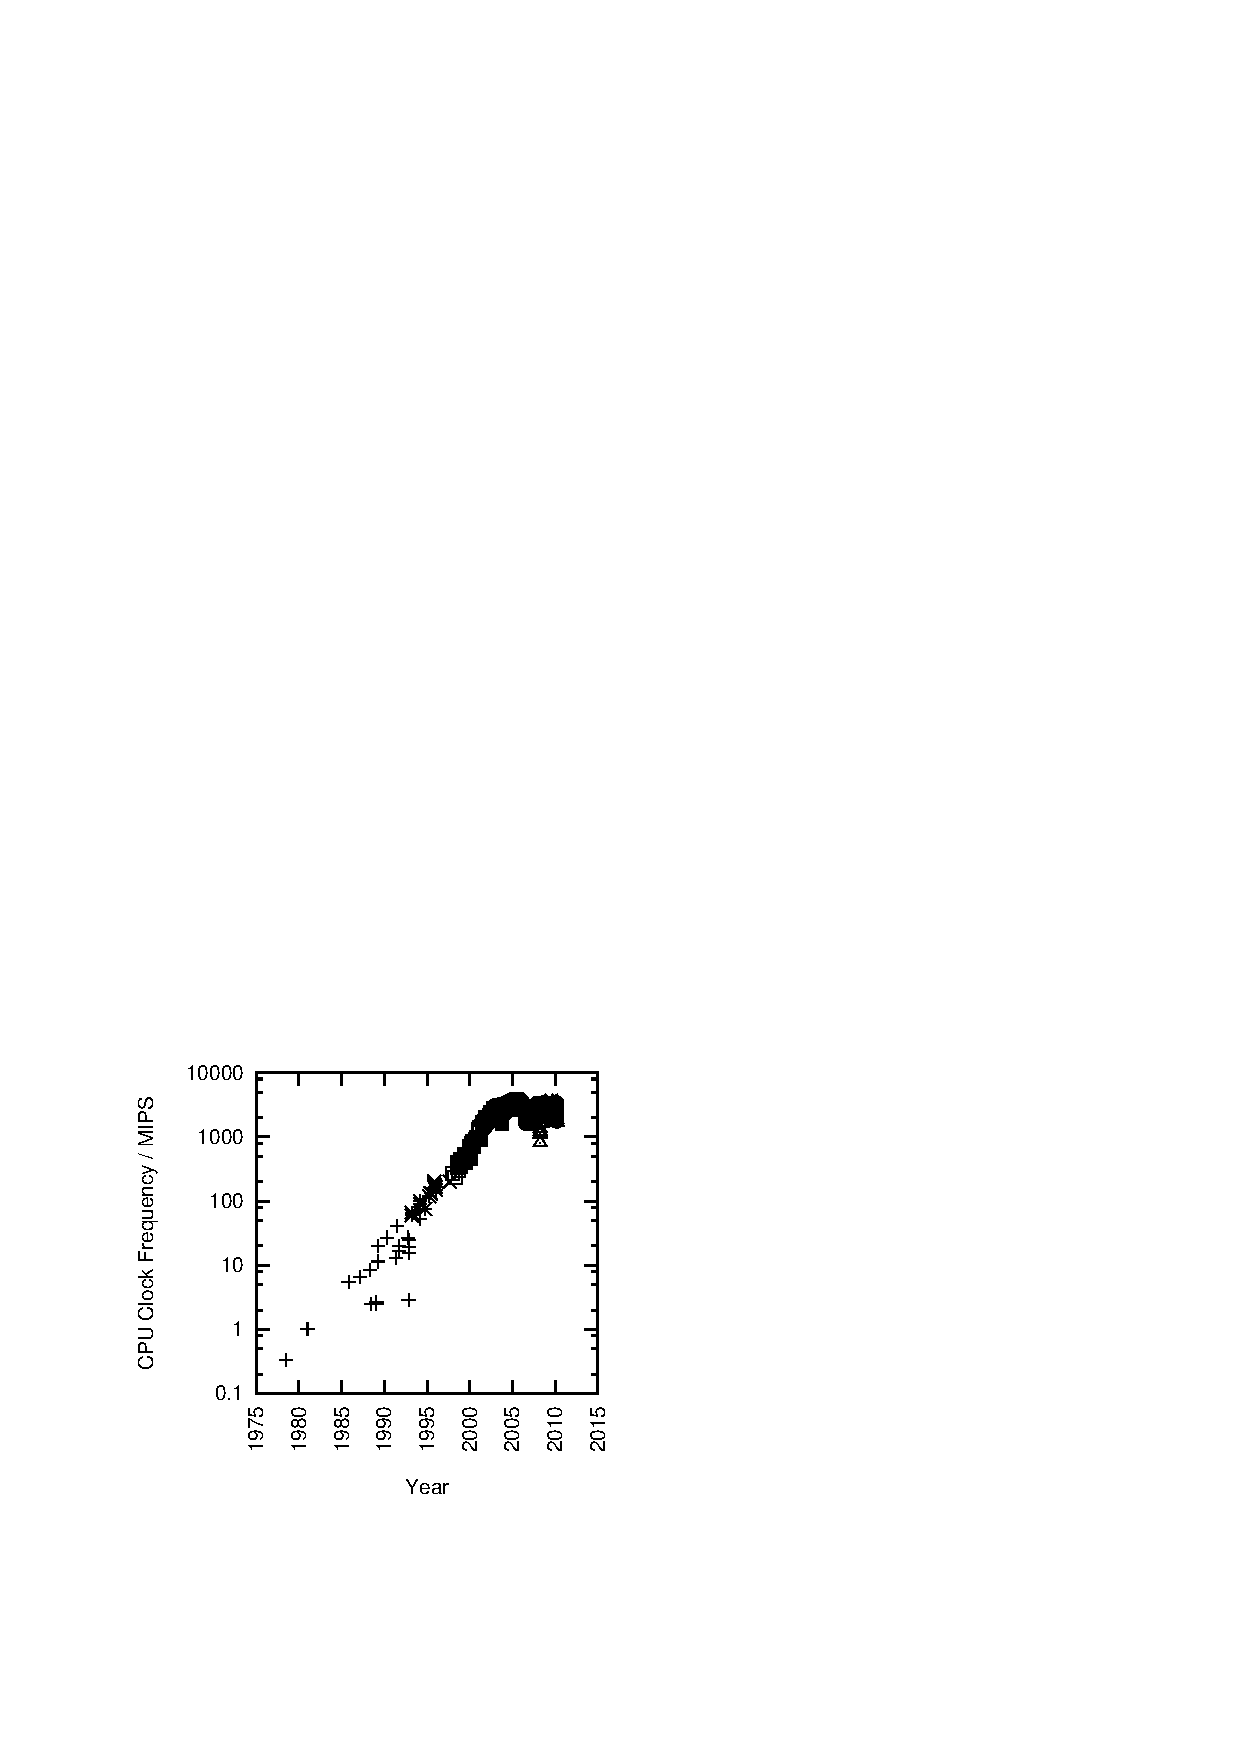
\includegraphics{SMPdesign/clockfreq}}
\end{center}
\caption{Clock-Frequency Trend for Intel CPUs}
\label{fig:intro:Clock-Frequency Trend for Intel CPUs}
\end{figure}

That said, the focus of performance has shifted from hardware to
parallel software.
This change in focus is due to the fact that Moore's Law has ceased to
provide its traditional performance
benefits, as can be seen in
Figure~\ref{fig:intro:Clock-Frequency Trend for Intel CPUs}.
This means that writing single-threaded code and simply waiting
a years or two for the CPUs to catch up may no longer be an option.
Given the recent trends on the part of all major manufacturers towards
multicore/multithreaded systems, parallelism is the way to go for
those wanting the avail themselves of the full performance of their
systems.

Even so, the first goal is performance rather than scalability,
especially given that the easiest way to attain linear scalability
is to reduce the performance of each CPU~\cite{LinusTorvalds2001a}.
Given a four-CPU system, which would you prefer?
A program that provides 100 transactions per second on a single CPU,
but does not scale at all?
Or a program that provides 10 transactions per second on a single CPU,
but scales perfectly?
The first program seems like a better bet, though the answer might
change if you happened to be one of the lucky few with access to a
32-CPU system.

That said, just because you have multiple CPUs is not necessarily
in and of itself a reason to use them all, especially given the
recent decreases in price of multi-CPU systems.
The key point to understand is that parallel programming is primarily
a performance optimization, and, as such, it is one potential optimization
of many.
If your program is fast enough as currently written, there is no
reason to optimize, either by parallelizing it or by applying any
of a number of potential sequential optimizations.\footnote{
	Of course, if you are a hobbyist whose primary interest is
	writing parallel software, that is more than reason enough to
	parallelize whatever software you are interested in.}

\subsection{Productivity}
\label{sec:intro:Productivity}

Productivity has been becoming increasingly important through the decades.
To see this, consider that early computers cost millions of dollars at
a time when engineering salaries were a few thousand dollars a year.
If dedicating a team of ten engineers to such a machine would improve
its performance by 10\%, their salaries would be repaid many times over.

One such machine was the CSIRAC, the oldest still-intact stored-program
computer, put in operation in
1949~\cite{CSIRACMuseumVictoria,CSIRACUniversityMelbourne}.
Given that the machine had but 768 words of RAM, it is safe to say
that the productivity issues that arise in large-scale software projects
were not an issue for this machine.
Because this machine was built before the transistor era, it was constructed
of 2,000 vacuum tubes, ran with a clock frequency of 1KHz,
consumed 30KW of power, and weighed more than three metric tons.

It would be difficult to purchase a machine with this little compute
power roughly sixty years later (2008), with the closest equivalents
being 8-bit embedded microprocessors exemplified by the venerable
Z80~\cite{z80Wikipedia}.
This CPU had 8,500 transistors, and can still be purchased in 2008
for less than \$2 US per unit in 1,000-unit quantities.
In stark contrast to the CSIRAC, software-development costs are
anything but insignificant for the Z80.

In short, one of the inescapable consequences of the rapid decrease in
the cost of hardware is that software productivity grows increasingly
important.
It is no longer sufficient merely to make efficient use of the hardware,
it is now also necessary to make extremely efficient use of software
developers.
This has long been the case for sequential hardware, but only recently
has parallel hardware become a low-cost commodity.
Therefore, the need for high productivity in creating parallel software
has only recently become hugely important.

\QuickQuiz{}
	Given how cheap parallel hardware has become, how can anyone
	afford to pay people to program it?
\QuickQuizAnswer{
	There are a number of answers to this question:
	\begin{enumerate}
	\item	Given a large computational cluster of parallel machines,
		the aggregate cost of the cluster can easily justify
		substantial developer effort, because the development
		cost can be spread over the large number of machines.
	\item	Popular software that is run by tens of millions of users
		can easily justify substantial developer effort,
		as the cost of this development can be spread over the tens
		of millions of users.
		Note that this includes things like kernels and system
		libraries.
	\item	If the low-cost parallel machine is controlling the operation
		of a valuable piece of equipment, then the cost of this
		piece of equipment might easily justify substantial
		developer effort.
	\item	If the software for the low-cost parallel produces an
		extremely valuable result (e.g., mineral exploration),
		then the valuable result might again justify substantial
		developer cost.
	\item	Safety-critical systems protect lives, which can clearly
		justify very large developer effort.
	\item	Hobbyists and researchers might seek knowledge, experience,
		fun, or glory rather than mere money.
	\end{enumerate}
	So it is not the case that the decreasing cost of hardware renders
	software worthless, but rather that it is no longer possible to
	``hide'' the cost of software development within the cost of
	the hardware, at least not unless there are extremely large
	quantities of hardware.
} \QuickQuizEnd

Perhaps at one time, the sole purpose of parallel software was performance.
Now, however, productivity is increasingly important.

\subsection{Generality}
\label{sec:intro:Generality}

One way to justify the high cost of developing parallel software
is to strive for maximal generality.
All else being equal, the cost of a more-general software artifact
can be spread over more users than can a less-general artifact.

Unfortunately, generality often comes at the cost of performance,
productivity, or both.
To see this, consider the following popular parallel programming
environments:

\begin{description}
\item[C/C++ ``Locking Plus Threads'']: This category, which includes
	POSIX Threads (pthreads)~\cite{OpenGroup1997pthreads},
	Windows Threads, and numerous
	operating-system kernel environments, offers excellent performance
	(at least within the confines of a single SMP system)
	and also offers good generality.
	Pity about the relatively low productivity.
\item[Java]: This programming environment, which is inherently
	multithreaded, is widely believed to be much more productive
	than C or C++, courtesy of the automatic garbage collector
	and the rich set of class libraries, and is reasonably
	general purpose.
	However, its performance, though greatly improved over the past ten
	years, is generally considered to be less than that of C and C++.
\item[MPI]: this message-passing interface~\cite{MPIForum2008} powers
	the largest scientific and technical computing clusters in
	the world, so offers unparalleled performance and scalability.
	It is in theory general purpose, but has generally been used
	for scientific and technical computing.
	It productivity is believed by many to be even less than that
	of C/C++ ``locking plus threads'' environments.
\item[OpenMP]: this set of compiler directives can be used
	to parallelize loops.  It is thus quite specific to this
	task, and this specificity often limits its performance,
	It is, however, much easier to use than MPI or parallel C/C++.
\item[SQL]: structured query language~\cite{DIS9075SQL92} is extremely
	specific, applying only to relational database queries.
	However, its performance is quite good, doing quite well
	in Transaction Processing Performance Council (TPC)
	benchmarks~\cite{TPC}.
	Productivity is excellent, in fact, this parallel programming
	environment permits people who know almost nothing about
	parallel programming to make good use of a large parallel
	machine.
\end{description}

\begin{figure}[tb]
\begin{center}
\resizebox{3in}{!}{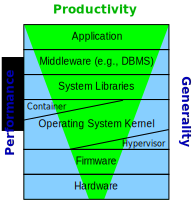
\includegraphics{intro/PPGrelation}}
\end{center}
\caption{Software Layers and Performance, Productivity, and Generality}
\label{fig:intro:Software Layers and Performance, Productivity, and Generality}
\end{figure}

The nirvana of parallel programming environments, one that offers
world-class performance, productivity, and generality, simply does
not yet exist.
Until such a nirvana appears, it will be necessary to make engineering
tradeoffs among performance, productivity, and generality.
One such tradeoff is shown in
Figure~\ref{fig:intro:Software Layers and Performance, Productivity, and Generality},
which shows how productivity becomes increasingly important at the upper layers
of the system stack,
while performance and generality become increasingly important at the
lower layers of the system stack.
The huge development costs incurred near the bottom of the stack
must be spread over equally huge numbers of users on the one hand
(hence the importance of generality), and
performance lost near the bottom of the stack cannot easily be
recovered further up the stack.
Near the top of the stack, there might be very few users for a given
specific application, in which case productivity concerns are paramount.
This explains the tendency towards ``bloatware'' further up the stack:
extra hardware is often cheaper than would be the extra developers.
Of course, this would in no way excuse bloat in any parallel applications
that have extremely large numbers of users!

It is important to note that a tradeoff between productivity and
generality has existed for centuries in many fields.
For but one example, a nailgun is far more productive than is a
hammer, but in contrast to the nailgun, a hammer can be used for
many things besides driving nails.
It should therefore be absolutely no surprise to see similar tradeoffs
appear in the field of parallel computing.

With the three parallel-programming goals of performance, productivity, 
and generality in mind, it is now time to look into alternatives to
parallel programming.

\section{Alternatives to Parallel Programming}
\label{sec:intro:Alternatives to Parallel Programming}

In order to properly consider alternatives to parallel programming,
you must first have thought through what you expect the parallelism
to do for you.
As seen in Section~\ref{sec:intro:Parallel Programming Goals},
the primary goals of parallel programming are performance, productivity,
and generality.

Although historically most parallel developers might be most concerned
with the first goal,
one advantage of the other goals is that they relieve you of the need
to justify using parallelism.
The remainder of this section is concerned only performance improvement.

It is important to keep in mind that parallelism is but one way to
improve performance.
Other well-known approaches include the following, in roughly increasing
order of difficulty:

\begin{enumerate}
\item	Run multiple instances of a sequential application.
\item	Construct the application to make use of existing parallel software.
\item	Apply performance optimization to the serial application.
\end{enumerate}

\subsection{Multiple Instances of a Sequential Application}
\label{sec:intro:Multiple Instances of a Sequential Application}

Running multiple instances of a sequential application can allow you
to do parallel programming without actually doing parallel programming.
There are a large number of ways to approach this, depending on the
structure of the application.

If your program is analyzing a large number of different scenarios,
or is analyzing a large number of independent data sets, one easy
and effective approach is to create a single sequential program that
carries out a single analysis, then use any of a number of scripting
enviroments (for example the \url{bash} shell) to run a number of
instances of this sequential program in parallel.
In some cases, this approach can be easily extended to a cluster of
machines.

This approach may seem like cheating, and in fact some denigrate such
programs ``embarrassingly parallel''.
And in fact, this approach does have some potential disadvantages,
including increased memory consumption, waste of CPU cycles recomputing
common intermediate results, and increased copying of data.
However, it is often  extremely effective, garnering extreme performance
gains with little or no added effort.

\subsection{Make Use of Existing Parallel Software}
\label{sec:intro:Make Use of Existing Parallel Software}

There is no longer any shortage of parallel software environments that
can present a single-threaded programming environment,
including relational
databases, web-application servers, and map-reduce environments.
For example, a common design provides a separate program for each
user, each of which generates SQL that is run against a common
relational database.
The per-user programs are responsible only for the user interface,
wiht hte relational database taking full responsbility for the
difficult issues surrounding parallelism and persistence.

\subsection{Performance Optimization}
\label{sec:intro:Performance Optimization}

Up through the early 2000s, CPU performance was doubling every 18 months.
In such an environment, it is often much more important to create new
functionality than to do careful performance optimization.
Now that Moore's Law is ``only'' increasing transistor density instead
of increasing both transistor density and per-transistor performance,
it might be a good time to rethink the importance of performance
optimization.

After all, performance optimization can reduce power consumption as
well as increasing performance.

Performance analysis of sequential programs is well understood,
and will not be discussed further here.
Instead, please note that parallel programming is but another performance
optimization, albeit one that is becoming \emph{much} more attractive
as parallel systems become cheaper and more readily available.

\section{Ease of Use}
\label{sec:intro:Ease of Use}

We are talking about parallel performance and latency,
so why is ease of use important?

Because the easier a performance technique is to use, the more likely
it will be used.
This greater use can outweigh a small performance penalty compared
to an optimal hard-to-use technique.
In addition, easier-to-use techniques usually improve productivity.

This book is not a collection of optimal algorithms with tiny areas of
applicability; instead, it is a handbook of widely applicable and heavily
used techniques.
We of course could not resist the urge to include some of our favorites
that have not (yet!) passed the test of time (what author could?), but
we have nonetheless gritted our teeth and banished our darlings to
appendices.
Perhaps in time, some of them will see enough use that we can promote
them into the main body of the text.

\section{Guide to This Book}
\label{sec:intro:Guide to This Book}

\emph{@@@ More here.  Sections.  Layered Approach.  Appendices.
Quick Quizzes.  Glossary.  Bibliography.}

\subsection{Quick Quizzes}

``Quick quizzes'' appear throughout this book.
Some of these quizzes are based on material in which that quick quiz
appears, but others require you to think beyond that section, and,
in some cases, beyond the entire book.
As with most endeavors, what you get out of this book is largely
determined by what you are willing to put into it.
Therefore, readers who invest some time into these quizzes will
find their effort repaid handsomely with increased understanding
of parallel programming.

Answers to the quizzes may be found
in
Appendix~\ref{chp:Answers to Quick Quizzes} starting on
page~\pageref{chp:Answers to Quick Quizzes}.

\QuickQuiz{}
	Where are the answers to the Quick Quizzes found?
\QuickQuizAnswer{
	In Appendix~\ref{chp:Answers to Quick Quizzes} starting on
	page~\pageref{chp:Answers to Quick Quizzes}.

	Hey, I thought I owed you an easy one!!!
} \QuickQuizEnd

\QuickQuiz{}
	Some of the Quick Quiz questions seem to be from the viewpoint
	of the reader rather than the author.
	Is that really the intent?
\QuickQuizAnswer{
	Indeed it is!
 	Many are modeled after Paul---just ask anyone who has had the
	misfortune of being assigned to teach him.
	Others are quite similar to actual questions that have been asked
	during conference presentations and lectures covering the
	material in this book.
	Still others are from the viewpoint of the author.
} \QuickQuizEnd

\subsection{Sample Source Code}

This book discusses its fair share of source code, and in many cases
this source code may be found in the \url{CodeSamples} directory
of this book's git tree.
For example, on UNIX systems, you should be able to type:
\begin{verbatim}
	find CodeSamples -name rcu_rcpls.c -print
\end{verbatim}
to locate the file \url{rcu_rcpls.c}, which is called out in
Section~\ref{defer:``Toy'' RCU Implementations}.
Other types of systems have well-known ways of locating files by
filename.

The source to this book may be found in the \url{git} archive at
\url{git://git.kernel.org/pub/scm/linux/kernel/git/paulmck/perfbook.git},
and \url{git} itself is available as part of most mainstream Linux
distributions.

% cpu/cpu.tex

\chapter{Hardware and its Habits}
\label{chp:Hardware and its Habits}

\QuickQuizChapter{chp:Hardware and its Habits}

Most people have an intuitive understanding that passing messages between
systems is considerably more expensive than performing simple calculations
within the confines of a single system.
However, it is not always so clear that communicating among threads within
the confines of a single shared-memory system can also be quite expensive.
This chapter therefore looks the cost of synchronization and communication
within a shared-memory system.
This chapter merely scratches the surface of shared-memory parallel
hardware design; readers desiring more detail would do well to start
with a recent edition of
Hennessy's and Patterson's classic text~\cite{Hennessy95a}.

% cpu/overview.tex

\section{Overview}
\label{sec:cpu:Overview}

Careless reading of computer-system specification sheets might lead one
to believe that CPU performance is a footrace on a clear track, as
illustrated in Figure~\ref{fig:cpu:CPU Performance at its Best},
where the race always goes to the swiftest.

\begin{figure}[htb]
\begin{center}
\resizebox{3in}{!}{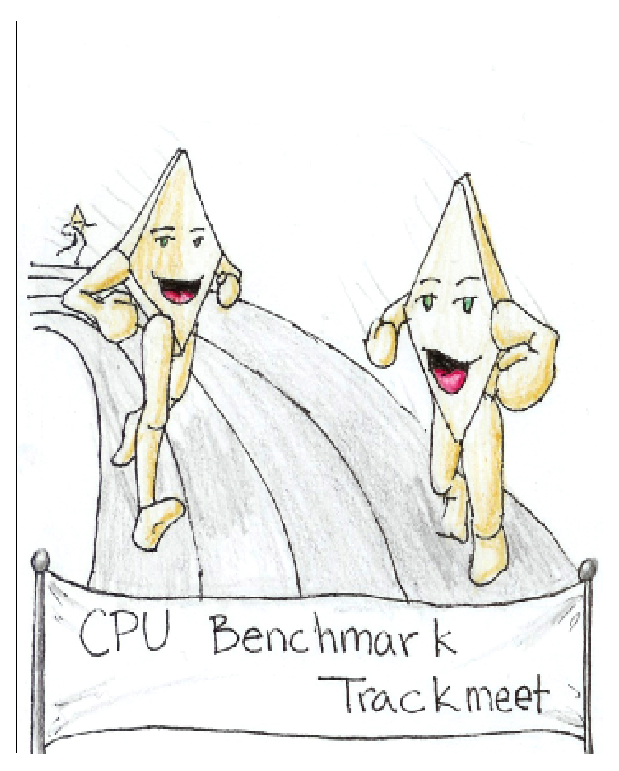
\includegraphics{cartoons/trackmeet}}
\end{center}
\caption{CPU Performance at its Best}
\ContributedBy{Figure}{fig:cpu:CPU Performance at its Best}{Melissa McKenney}
\end{figure}

Although there are a few CPU-bound benchmarks that approach the ideal
shown in Figure~\ref{fig:cpu:CPU Performance at its Best},
the typical program more closely resembles an obstacle course than
a race track.
This is because the internal architecture of CPUs has changed dramatically
over the past few decades, courtesy of Moore's Law.
These changes are described in the following sections.

\subsection{Pipelined CPUs}
\label{sec:cpu:Pipelined CPUs}

\begin{figure}[htb]
\begin{center}
\resizebox{3in}{!}{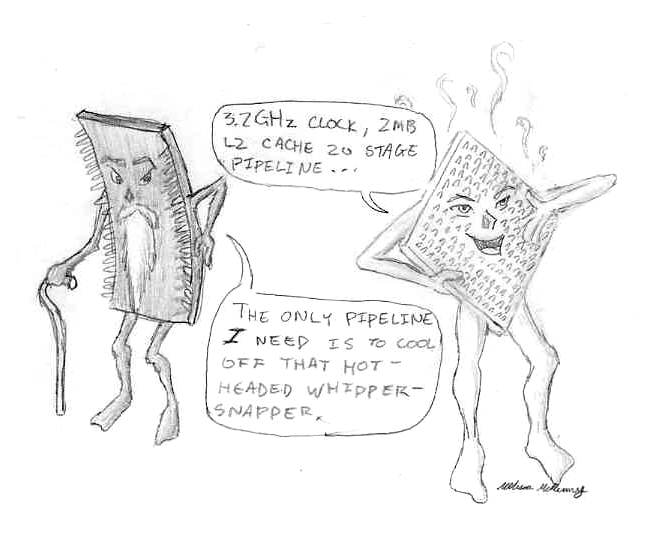
\includegraphics{cartoons/whippersnapper}}
\end{center}
\caption{CPUs Old and New}
\ContributedBy{Figure}{fig:cpu:CPUs Old and New}{Melissa McKenney}
\end{figure}

In the early 1980s, the typical microprocessor fetched an instruction,
decoded it, and executed it, typically taking \emph{at least} three
clock cycles to complete one instruction before proceeding to the next.
In contrast, the CPU of the late 1990s and early 2000s will be executing
many instructions simultaneously, using a deep ``pipeline'' to control
the flow of instructions internally to the CPU, this difference being
illustrated by Figure~\ref{fig:cpu:CPUs Old and New}.

Achieving full performance with a CPU having a long pipeline requires
highly predictable control flow through the program.
Suitable control flow can be provided by a program that executes primarily
in tight loops, for example, programs doing arithmetic on large matrices
or vectors.
The CPU can then correctly predict that the branch at the end of the loop
will be taken in almost all cases.
In such programs, the pipeline can be kept full and the CPU can execute
at full speed.

\begin{figure}[htb]
\begin{center}
\resizebox{3in}{!}{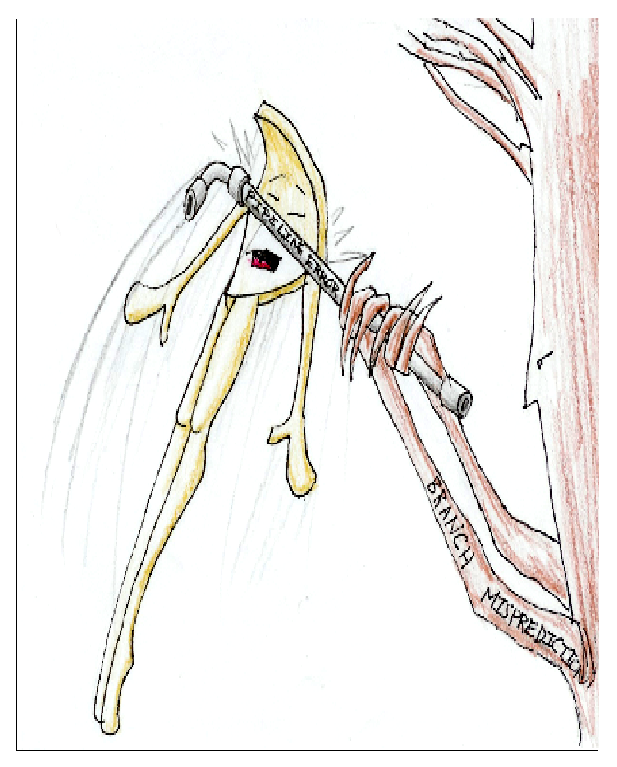
\includegraphics{cartoons/pipeline}}
\end{center}
\caption{CPU Meets a Pipeline Flush}
\ContributedBy{Figure}{fig:cpu:CPU Meets a Pipeline Flush}{Melissa McKenney}
\end{figure}

If, on the other hand, the program has many loops with small loop counts,
or if the program is object oriented with many virtual objects that
can reference many different real objects, all with different implementations
for frequently invoked member functions, then it is difficult or even
impossible for the CPU to predict where a given branch might lead.
The CPU must then either stall waiting for execution to proceed far enough
to know for certain where the branch will lead, or guess --- and, in the
face of programs with unpredictable control flow, frequently guess wrong.
In either case, the pipeline will empty and have to be refilled, leading
to stalls that can drastically reduce performance,
as fancifully depicted in Figure~\ref{fig:cpu:CPU Meets a Pipeline Flush}.

Unfortunately, pipeline flushes are not the only hazards in the obstacle
course that modern CPUs must run.
The next section covers the hazards of referencing memory.

\subsection{Memory References}
\label{sec:cpu:Memory References}

In the 1980s, it often took less time for a microprocessor to load a value
from memory than it did to execute an instruction.
In 2006, a microprocessor might be capable of executing hundreds or even
thousands of instructions in the time required to access memory.
This disparity is due to the fact that Moore's Law has increased CPU
performance at a much greater rate than it has increased memory
performance, in part due to the rate at which memory sizes have
grown.
For example, a typical 1970s minicomputer might have 4KB (yes, kilobytes,
not megabytes, let alone gigabytes) of main memory, with single-cycle access.
In 2008, CPU designers still can construct a 4KB memory with single-cycle
access, even on systems with multi-GHz clock frequencies.
And in fact they frequently do construct such memories, but they now
call them ``level-0 caches''.

Although the large caches found on modern microprocessors can do quite
a bit to help combat memory-access latencies,
these caches require highly predictable data-access patterns to
successfully hide memory latencies.
Unfortunately, common operations, such as traversing a linked list,
have extremely unpredictable memory-access patterns --- after all,
if the pattern was predictable, us software types would not bother
with the pointers, right?

\begin{figure}[htb]
\begin{center}
\resizebox{3in}{!}{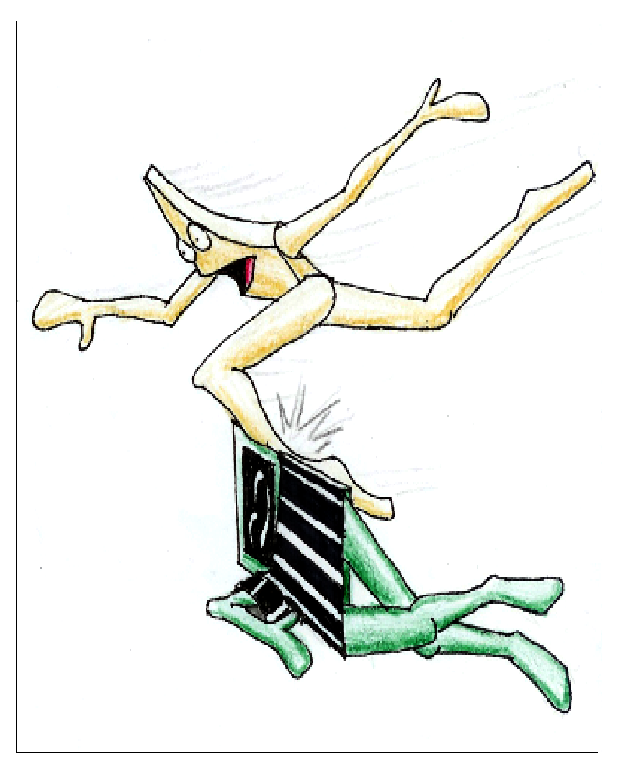
\includegraphics{cartoons/ref}}
\end{center}
\caption{CPU Meets a Memory Reference}
\ContributedBy{Figure}{fig:cpu:CPU Meets a Memory Reference}{Melissa McKenney}
\end{figure}

Therefore, as shown in
Figure~\ref{fig:cpu:CPU Meets a Memory Reference},
memory references are often severe obstacles for modern CPUs.

Thus far, we have only been considering obstacles that can arise during
a given CPU's execution of single-threaded code.
Multi-threading presents additional obstacles to the CPU, as
described in the following sections.

\subsection{Atomic Operations}
\label{sec:cpu:Atomic Operations}

One such obstacle is atomic operations.
The whole idea of an atomic operation in some sense conflicts with
the piece-at-a-time assembly-line operation of a CPU pipeline.
To hardware designers' credit, modern CPUs use a number of extremely clever
tricks to make such operations \emph{look} atomic even though they
are in fact being executed piece-at-a-time, but even so, there are
cases where the pipeline must be delayed or even flushed in order to
permit a given atomic operation to complete correctly.

\begin{figure}[htb]
\begin{center}
\resizebox{3in}{!}{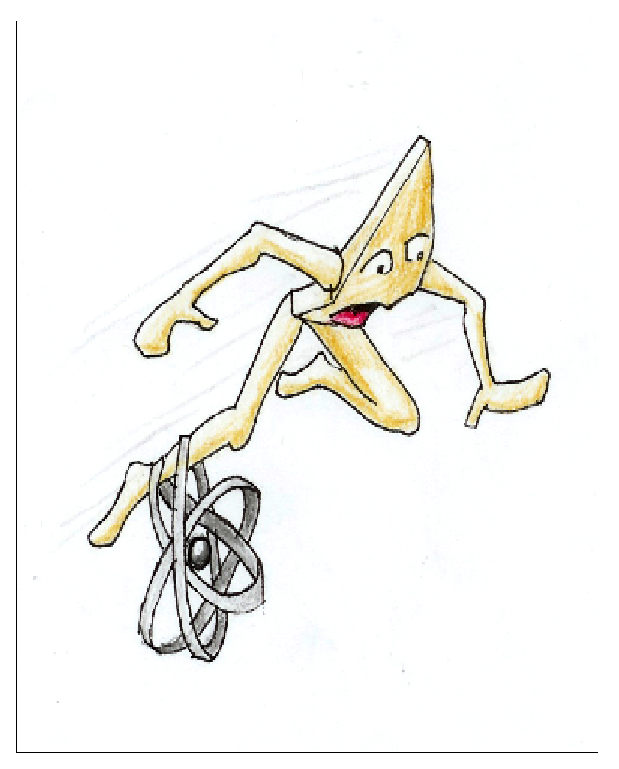
\includegraphics{cartoons/atomic}}
\end{center}
\caption{CPU Meets an Atomic Operation}
\ContributedBy{Figure}{fig:cpu:CPU Meets an Atomic Operation}{Melissa McKenney}
\end{figure}

The resulting effect on performance is depicted in
Figure~\ref{fig:cpu:CPU Meets an Atomic Operation}.

Unfortunately, atomic operations usually apply only to single elements
of data.
Because many parallel algorithms require that ordering constraints
be maintained between updates of multiple data elements, most CPUs
provide memory barriers.
These memory barriers also serve as performance-sapping obstacles,
as described in the next section.

\QuickQuiz{}
	What types of machines would allow atomic operations on
	multiple data elements?
\QuickQuizAnswer{
	One answer to this question is that it is often possible to
	pack multiple elements of data into a single machine word,
	which can then be manipulated atomically.

	A more trendy answer would be machines supporting transactional
	memory~\cite{DBLomet1977SIGSOFT}.
	However, such machines are still (as of 2008) research
	curiosities.
	The jury is still out on the applicability of transactional
	memory~\cite{McKenney2007PLOSTM,DonaldEPorter2007TRANSACT,
	ChistopherJRossbach2007a}.
} \QuickQuizEnd

\subsection{Memory Barriers}
\label{sec:cpu:Memory Barriers}

Memory barriers will be considered in more detail in
Section~\ref{sec:advsync:Memory Barriers} and
Appendix~\ref{chp:app:whymb:Why Memory Barriers?}.
In the meantime, consider the following simple lock-based critical
section:

\vspace{5pt}
\begin{minipage}[t]{\columnwidth}
\small
\begin{verbatim}
  1 spin_lock(&mylock);
  2 a = a + 1;
  3 spin_unlock(&mylock);
\end{verbatim}
\end{minipage}
\vspace{5pt}

\begin{figure}[tb]
\begin{center}
\resizebox{3in}{!}{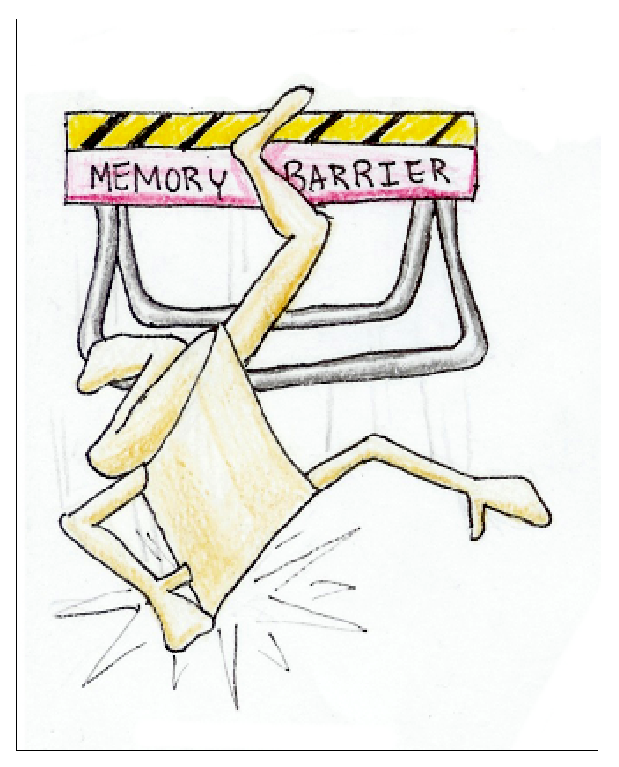
\includegraphics{cartoons/barrier}}
\end{center}
\caption{CPU Meets a Memory Barrier}
\ContributedBy{Figure}{fig:cpu:CPU Meets a Memory Barrier}{Melissa McKenney}
\end{figure}

If the CPU were not constrained to execute these statements in the
order shown, the effect would be that the variable ``a'' would be
incremented without the protection of ``mylock'', which would certainly
defeat the purpose of acquiring it.
To prevent such destructive reordering, locking primitives contain
either explicit or implicit memory barriers.
Because the whole purpose of these memory barriers is to prevent reorderings
that the CPU would otherwise undertake in order to increase performance,
memory barriers almost always reduce performance, as depicted in
Figure~\ref{fig:cpu:CPU Meets a Memory Barrier}.

\subsection{Cache Misses}
\label{sec:cpu:Cache Misses}

\begin{figure}[htb]
\begin{center}
\resizebox{3in}{!}{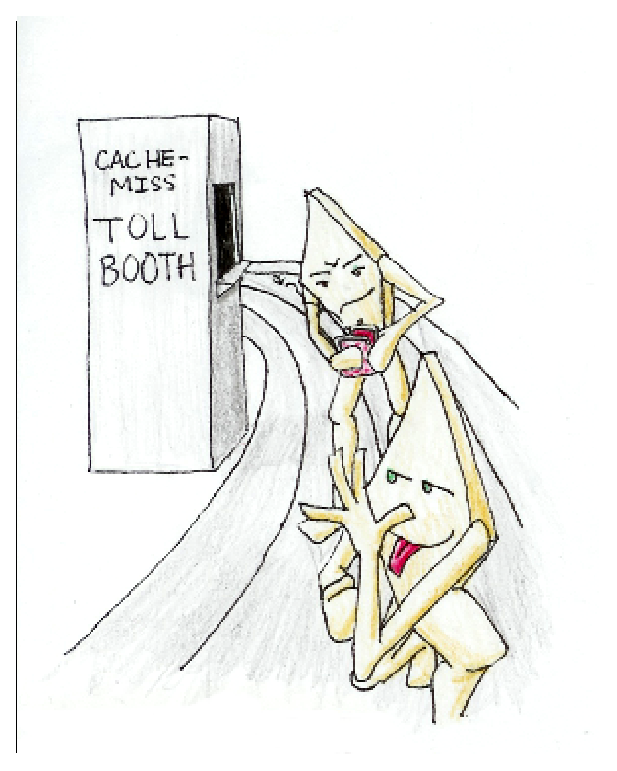
\includegraphics{cartoons/tollbooth}}
\end{center}
\caption{CPU Meets a Cache Miss}
\ContributedBy{Figure}{fig:cpu:CPU Meets a Cache Miss}{Melissa McKenney}
\end{figure}

An additional multi-threading obstacle to CPU performance is
the ``cache miss''.
As noted earlier, modern CPUs sport large caches in order to reduce the
performance penalty that would otherwise be incurred due to high memory
latencies.
However, these caches are actually counter-productive for variables that
are frequently shared among CPUs.
This is because when a given CPU wishes to modify the variable, it is
most likely the case that some other CPU has modified it recently.
In this case, the variable will be in that other CPU's cache, but not
in this CPU's cache, which will therefore incur an expensive cache miss
(see Section~\ref{sec:app:whymb:Cache Structure} for more detail).
Such cache misses form a major obstacle to CPU performance, as shown
in Figure~\ref{fig:cpu:CPU Meets a Cache Miss}.

\subsection{I/O Operations}
\label{sec:cpu:I/O Operations}

\begin{figure}[htb]
\begin{center}
\resizebox{3in}{!}{\includegraphics{cartoons/PhoneBooth}}
\end{center}
\caption{CPU Waits for I/O Completion}
\ContributedBy{Figure}{fig:cpu:CPU Waits for I/O Completion}{Melissa McKenney}
\end{figure}

A cache miss can be thought of as a CPU-to-CPU I/O operation, and as
such is one of the cheapest I/O operations available.
I/O operations involving networking, mass storage, or (worse yet) human
beings pose much greater obstacles than the internal obstacles called
out in the prior sections,
as illustrated by
Figure~\ref{fig:cpu:CPU Waits for I/O Completion}.

This is one of the differences between shared-memory and distributed-system
parallelism: shared-memory parallel programs must normally deal with no
obstacle worse than a cache miss, while a distributed parallel program
will typically incur the larger network communication latencies.
In both cases, the relevant latencies can be thought of as a cost of
communication---a cost that would be absent in a sequential program.
Therefore, the ratio between the overhead of the communication to
that of the actual work being performed is a key design parameter.
A major goal of parallel design is to reduce this ratio as needed to
achieve the relevant performance and scalability goals.

Of course, it is one thing to say that a given operation is an obstacle,
and quite another to show that the operation is a \emph{significant}
obstacle.
This distinction is discussed in the following sections.


% @@@ table capturing latencies, toilet-paper analogy.

\section{Logical Components}
\label{sec:cpu:Logical Components}

\section{Instruction Execution and Ordering}
\label{sec:cpu:Instruction Execution and Ordering}

\section{Caching and Memory Access Ordering}
\label{sec:cpu:Caching and Memory Access Ordering}

\section{Memory Windows, MMIO, and Caching}
\label{sec:cpu:Memory Windows, MMIO, and Caching}

\section{Memory Alignment}
\label{sec:cpu:Memory Alignment}

% toolsoftrade/toolsoftrade.tex

\chapter{Tools of the Trade}
\label{chp:Tools of the Trade}

\QuickQuizChapter{chp:Tools of the Trade}

This chapter provides a brief introduction to some basic tools of the
parallel-programming trade, focusing mainly on those available to
user applications running on operating systems similar to Linux.
Section~\ref{sec:toolsoftrade:Scripting Languages} begins with
scripting languages,
Section~\ref{sec:toolsoftrade:POSIX Multiprocessing}
describes the multi-process parallelism supported by the POSIX API,
Section~\ref{sec:toolsoftrade:POSIX Multiprocessing} touches on POSIX threads,
and finally,
Section~\ref{sec:toolsoftrade:Atomic Operations}
describes atomic operations.

Please note that this chapter provides but a brief introduction.
More detail is available from the references cited, and more information
on how best to use these tools will be provided in later chapters.

\section{Scripting Languages}
\label{sec:toolsoftrade:Scripting Languages}

The Linux shell scripting languages provide simple but effective ways
of managing parallelism.
For example, suppose that you had a program \url{compute_it}
that you needed to run twice with two different sets of arguments.
This can be accomplished as follows:

\vspace{5pt}
\begin{minipage}[t]{\columnwidth}
\begin{verbatim}
  1 compute_it 1 > compute_it.1.out &
  2 compute_it 2 > compute_it.2.out &
  3 wait
  4 cat < compute_it.1.out
  5 cat < compute_it.2.out
\end{verbatim}
\end{minipage}
\vspace{5pt}

Lines~1 and 2 launch two instances of this program, redirecting their
output to two separate files, with the \url{&} character directing the
shell to run the two instances of the program in the background.
Line~3 waits for both instances to complete, and lines~4 and 5
display their output.
% @@@ Maui scheduler, load balancing, BOINC, and so on.

\QuickQuiz{}
	But this silly shell script isn't a \emph{real} parallel program!!!
	Why bother with such trivia???
\QuickQuizAnswer{
	Because you should \emph{never} forget the simple stuff!!!

	Please keep in mind that the title of this book is
	``Is Parallel Programming Hard, And, If So, What Can You Do About It?''.
	One of the most effective things you can do about it is to
	avoid forgetting the simple stuff!
	After all, if you choose to do parallel programming the hard
	way, you have no one but yourself to blame for it being hard.
} \QuickQuizEnd

\QuickQuiz{}
	Is there a simpler way to create a parallel shell script?
	If so, how?  If not, why not?
\QuickQuizAnswer{
	One straightforward approach is the shell pipeline:
\vspace{5pt}
\begin{minipage}[t]{\columnwidth}
\small
\begin{verbatim}
grep $pattern1 | sed -e 's/a/b/' | sort
\end{verbatim}
\end{minipage}
\vspace{5pt}
	For a sufficiently large input file,
	\url{grep} will pattern-match in parallel with \url{sed}
	editing and with the input processing of \url{sort}.
	See the file \url{parallel.sh} for a demonstration of
	shell-script parallelism and pipelining.
} \QuickQuizEnd

For another example, the \url{make} software-build scripting language
provides a \url{-j} option that specifies how much parallelism should be
introduced into the build process.
For example, typing \url{make}~\url{-j4} when building a Linux kernel
specifies that up to four parallel compiles be carried out concurrently.

It is hoped that these simple examples convince you that parallel
programming need not always be complex or difficult.

\QuickQuiz{}
	But if script-based parallel programming is so easy, why
	bother with anything else?
\QuickQuizAnswer{
	In fact, it is quite likely that a very large fraction of
	parallel programs in use today are script-based.
	However, script-based parallelism does have its limitations:
	\begin{enumerate}
	\item	Creation of new processes is usually quite heavyweight,
		involving the expensive \url{fork()} and \url{exec()}
		system calls.
	\item	Sharing of data, including pipelining, typically involves
		expensive file I/O.
	\item	The reliable synchronization primitives available to
		scripts also typically involve expensive file I/O.
	\end{enumerate}
	These limitations require that script-based parallelism use
	coarse-grained parallelism, with each unit of work having
	execution time of at least tens of milliseconds, and preferably
	much longer.

	Those requiring finer-grained parallelism are well advised to
	think hard about their problem to see if it can be expressed
	in a coarse-grained form.
	If not, they should consider using other parallel-programming
	environments, such as those discussed in
	Section~\ref{sec:toolsoftrade:POSIX Multiprocessing}.
} \QuickQuizEnd

\section{POSIX Multiprocessing}
\label{sec:toolsoftrade:POSIX Multiprocessing}

This section scratches the surface of the
POSIX environment, including pthreads~\cite{OpenGroup1997pthreads},
as this environment is readily available and widely implemented.
Section~\ref{sec:toolsoftrade:POSIX Process Creation and Destruction}
provides a glimpse of the POSIX \url{fork()} and related primitives,
Section~\ref{sec:toolsoftrade:POSIX Thread Creation and Destruction}
touches on thread creation and distruction,
Section~\ref{sec:toolsoftrade:POSIX Locking} gives a brief overview
of POSIX locking, and, finally,
Section~\ref{sec:toolsoftrade:Linux-Kernel Equivalents to POSIX Operations}
presents the analogous operations within the Linux kernel.

\subsection{POSIX Process Creation and Destruction}
\label{sec:toolsoftrade:POSIX Process Creation and Destruction}

Processes are created using the \url{fork()} primitive, they may
be destroyed using the \url{kill()} primitive, they may destroy
themselves using the \url{exit()} primitive.
A process executing a \url{fork()} primitive is said to be the ``parent''
of the newly created process.
A parent may wait on its children using the \url{wait()} primitive.

Please note that the examples in this section are quite simple.
Real-world applications using these primitives might need to manipulate
signals, file descriptors, shared memory segments, and any number of
other resources.
In addition, some applications need to take specific actions if a given
child terminates, and might also need to be concerned with the reason
that the child terminated.
These concerns can of course add substantial complexity to the code.

\begin{figure}[tbp]
{ \scriptsize
\begin{verbatim}
  1 pid = fork();
  2 if (pid == 0) {
  3   /* child */
  4 } else if (pid < 0) {
  5   /* parent, upon error */
  6   perror("fork");
  7   exit(-1);
  8 } else {
  9   /* parent, pid == child ID */
 10 }
\end{verbatim}
}
\caption{Using the fork() Primitive}
\label{fig:toolsoftrade:Using the fork() Primitive}
\end{figure}

If \url{fork()} succeeds, it returns twice, once for the parent
and again for the child.
The value returned from \url{fork()} allows the caller to tell
the difference, as shown in
Figure~\ref{fig:toolsoftrade:Using the fork() Primitive}.
Line~1 executes the \url{fork()} primitive, and saves its return value
in local variable \url{pid}.
Line~2 checks to see if \url{pid} is zero, in which case, this is the
child, which continues on to execute line~3.
As noted earlier, the child may terminate via the \url{exit()} primitive.
Otherwise, this is the parent, which checks for an error return from
the \url{fork()} primitive on line~4, and prints an error and exits
on lines~5-7 if so.
Otherwise, the \url{fork()} has executed successfully, and the parent
therefore executes line 9 with the variable \url{pid} containing the
process ID of the child.

\begin{figure}[tbp]
{ \scriptsize
\begin{verbatim}
  1 void waitall(void)
  2 {
  3   int pid;
  4   int status;
  5 
  6   for (;;) {
  7     pid = wait(&status);
  8     if (pid == -1) {
  9       if (errno == ECHILD)
 10         break;
 11       perror("wait");
 12       exit(-1);
 13     }
 14   }
 15 }
\end{verbatim}
}
\caption{Using the wait() Primitive}
\label{fig:toolsoftrade:Using the wait() Primitive}
\end{figure}

The parent process may use the \url{wait()} primitive to wait for its children
to complete.
However, use of this primitive is a bit more complicated than its shell-script
counterpart, as each invocation of \url{wait()} waits for but one child
process.
It is therefore customary to wrap \url{wait()} into a function similar
to the \url{waitall()} function shown in
Figure~\ref{fig:toolsoftrade:Using the wait() Primitive},
this \url{waitall()} function having semantics similar to the
shell-script \url{wait} command.
Each pass through the loop spanning lines~6-15 waits on one child process.
Line~7 invokes the \url{wait()} primitive, which blocks until a child process
exits, and returns that child's process ID.
If the process ID is instead -1, this indicates that the \url{wait()}
primitive was unable to wait on a child.
If so, line~9 checks for the \url{ECHILD} errno, which indicates that there
are no more child processes, so that line~10 exits the loop.
Otherwise, lines~11 and 12 print an error and exit.

\QuickQuiz{}
	Why does this \url{wait()} primitive need to be so complicated?
	Why not just make it work like the shell-script \url{wait} does?
\QuickQuizAnswer{
	Some parallel applications need to take special action when
	specific children exit, and therefore need to wait for each
	child individually.
	In addition, some parallel applications need to detect the
	reason that the child died.
	As we saw in Figure~\ref{fig:toolsoftrade:Using the wait() Primitive},
	it is not hard to build a \url{waitall()} function out of
	the \url{wait()} function, but it would be impossible to
	do the reverse.
	Once the information about a specific child is lost, it is lost.
} \QuickQuizEnd

\begin{figure}[tbp]
{ \scriptsize
\begin{verbatim}
  1 int x = 0;
  2 int pid;
  3 
  4 pid = fork();
  5 if (pid == 0) { /* child */
  6   x = 1;
  7   printf("Child process set x=1\n");
  8   exit(0);
  9 }
 10 if (pid < 0) { /* parent, upon error */
 11   perror("fork");
 12   exit(-1);
 13 }
 14 waitall();
 15 printf("Parent process sees x=%d\n", x);
\end{verbatim}
}
\caption{Processes Created Via fork() Do Not Share Memory}
\label{fig:toolsoftrade:Processes Created Via fork() Do Not Share Memory}
\end{figure}

It is critically important to note that the parent and child do \url{not}
share memory.
This is illustrated by the program shown in
Figure~\ref{fig:toolsoftrade:Processes Created Via fork() Do Not Share Memory},
in which the child sets a global variable \url{x} to 1 on line~6,
prints a message on line~7, and exits on line~8.
The parent continues at line~14, where it waits on the child,
and on line~15 finds that its copy of the variable \url{x} is still zero.

\QuickQuiz{}
	Isn't there a lot more to \url{fork()} and \url{wait()}
	than discussed here?
\QuickQuizAnswer{
	Indeed there is!
	There are any number of textbooks that cover these primitives
	in great detail,
	and the truly motivated can read manpages, existing parallel
	applications using these primitives, as well as the
	Linux-kernel implementations.
} \QuickQuizEnd

The finest-grained parallelism of course requires shared memory, and
this is covered in
Section~\ref{sec:toolsoftrade:POSIX Thread Creation and Destruction}.
That said, shared-memory parallelism can be significantly more complex
than fork-join parallelism.

\subsection{POSIX Thread Creation and Destruction}
\label{sec:toolsoftrade:POSIX Thread Creation and Destruction}

\url{pthread_create()}

\url{pthread_exit()}

\url{pthread_join()}

\subsection{POSIX Locking}
\label{sec:toolsoftrade:POSIX Locking}

\url{pthread_mutex_lock()}

\url{pthread_mutex_unlock()}

\subsection{Linux-Kernel Equivalents to POSIX Operations}
\label{sec:toolsoftrade:Linux-Kernel Equivalents to POSIX Operations}

\section{Atomic Operations}
\label{sec:toolsoftrade:Atomic Operations}

% count/count.tex

\chapter{Counting}
\label{chp:Counting}

\QuickQuizChapter{chp:Counting}

Counting may seem like the easiest and most natural arithmetic operation
possible.
However, doing so in an efficient and scalable manner on a large
shared-memory multiprocessor can be quite challenging.
This chapter covers a number of special cases for which there are simple,
fast, and scalable counting algorithms.
But first, let us find out how much you already know about concurrent
counting.

\QuickQuiz{}
	Why on earth should efficient and scalable counting be hard???
\QuickQuizAnswer{
	Because the straightforward counting algorithms, for example,
	atomic operations on a shared counter, are slow and scale
	very badly, as will be seen in Section @@@.
} \QuickQuizEnd

\QuickQuiz{}
	Suppose that you need to collect statistics on the number
	of networking packets (or total number of bytes) transmitted
	and/or received.
	Packets might be transmitted or received by any CPU on
	the system.
	Suppose further that this large machine is capable of
	handling a million packets per second, and that there
	is a systems-monitoring package that reads out the count
	every five seconds.
	How would you implement this statistical counter?
\QuickQuizAnswer{
	Hint: the act of updating the counter must be blazingly
	fast, but because the counter is read out only about once
	in five million updates, the act of reading out the counter can be
	quite slow.
	In addition, the value read out normally need not be all that
	accurate---after all, since the counter is updated a thousand
	times per millisecond, we should be able to work with a value
	that is within a few thousand counts of the ``true value'',
	whatever ``true value'' might mean in this context.
	However, the value read out should maintain roughly the same
	absolute error over time.
	For example, while a 1\% error might be OK when the count
	is on the order of a million or so, it is absolutely unacceptable
	once the count reaches a trillion.
	See Section @@@.
} \QuickQuizEnd

\QuickQuiz{}
	Suppose that you need to maintain a reference count on a
	heavily used removable mass-storage device, so that you
	can tell the user when it is safe to removed the device.
	This device follows the usual removal procedure where
	the user indicates a desire to remove the device, and
	the system tells the user when it is safe to do so.
\QuickQuizAnswer{
	Hint: the act of updating the counter must be blazingly
	fast, but because the counter is read out only when the
	user wishes to remove the device, the counter read-out
	operation can be extremely slow.
	Furthermore, there is no need to be able to read out
	the counter at all unless the user has already indicated
	a desire to remove the device.
	In addition, the value read out need not be accurate
	\emph{except} that it absolutely must distinguish perfectly
	between non-zero and zero values.
	See Section @@@.
} \QuickQuizEnd

\QuickQuiz{}
	Suppose that you need to maintain a count of the number of
	structures allocated in order to fail any allocations
	once the number of structures in use exceeds a limit
	(say, 10,000).
	Suppose further that these structures are short-lived,
	and that the limit is rarely exceeded.
\QuickQuizAnswer{
	Hint: the act of updating the counter must be blazingly
	fast, but the counter is read out each time that the
	counter is increased.
	However, the value read out need not be accurate
	\emph{except} that it absolutely must distinguish perfectly
	between values below the limit and values greater than or
	equal to the limit.
	See Section @@@.
} \QuickQuizEnd

% SMPdesign/SMPdesign.tex

\QuickQuizChapter{cha:Partitioning and Synchronization Design}{Partitioning and Synchronization Design}

This chapter describes how to design software to take advantage of
the multiple CPUs that are increasingly appearing in commodity systems.
It does this by presenting a number of idioms, or
``design patterns''~\cite{Alexander79,GOF95,SchmidtStalRohnertBuschmann2000v2Textbook}
that can help you balance performance, scalability, and response time.
As noted in earlier chapters, the most important decision you will make
when creating parallel software is how to carry out the partitioning.
Correctly partitioned problems lead to simple, scalable, and
high-performance solutions, while poorly partitioned problems result
in slow and complex solutions.
This chapter will help you design partitioning into your code, with
some discussion of batching and weakening as well.
The word ``design'' is very important: You should partition first,
batch second, weaken third, and code fourth.
Changing this order often leads to poor performance and scalability
along with great frustration.

To this end, Section~\ref{sec:SMPdesign:Partitioning Exercises}
presents partitioning exercises,
Section~\ref{sec:SMPdesign:Design Criteria} reviews partitionability
design criteria,
Section~\ref{sec:SMPdesign:Synchronization Granularity}
discusses selecting an appropriate synchronization granularity,
Section~\ref{sec:SMPdesign:Parallel Fastpath}
gives an overview of important parallel-fastpath designs
that provide speed and scalability in the common case with
a simpler but less-scalable fallback ``slow path'' for unusual
situations,
and finally
Section~\ref{sec:SMPdesign:Beyond Partitioning}
takes a brief look beyond partitioning.

% SMPdesign/partexercises.tex

\section{Partitioning Exercises}
\label{sec:SMPdesign:Partitioning Exercises}

This section uses a pair of exercises (the classic Dining Philosophers
problem and a double-ended queue) to demonstrate the value of partitioning.

\subsection{Dining Philosophers Problem}
\label{sec:SMPdesign:Dining Philosophers Problem}

\begin{figure}[tb]
\begin{center}
\includegraphics[scale=.7]{SMPdesign/DiningPhilosopher5}
\end{center}
\caption{Dining Philosophers Problem}
\ContributedBy{Figure}{fig:SMPdesign:Dining Philosophers Problem}{Kornilios Kourtis}
\end{figure}

Figure~\ref{fig:SMPdesign:Dining Philosophers Problem} shows a diagram
of the classic Dining Philosophers problem~\cite{Dijkstra1971HOoSP}.
This problem features five philosophers who do nothing but think and
eat a ``very difficult kind of spaghetti'' which requires two forks
to eat.
A given philosopher is permitted to use only the forks to his or her
immediate right and left, and once a philosopher picks up a fork,
he or she will not put it down until sated.\footnote{
	Readers who have difficulty imagining a food that requires
	two forks are invited to instead think in terms of chopsticks.}

\begin{figure*}[tb]
\begin{center}
\resizebox{5in}{!}{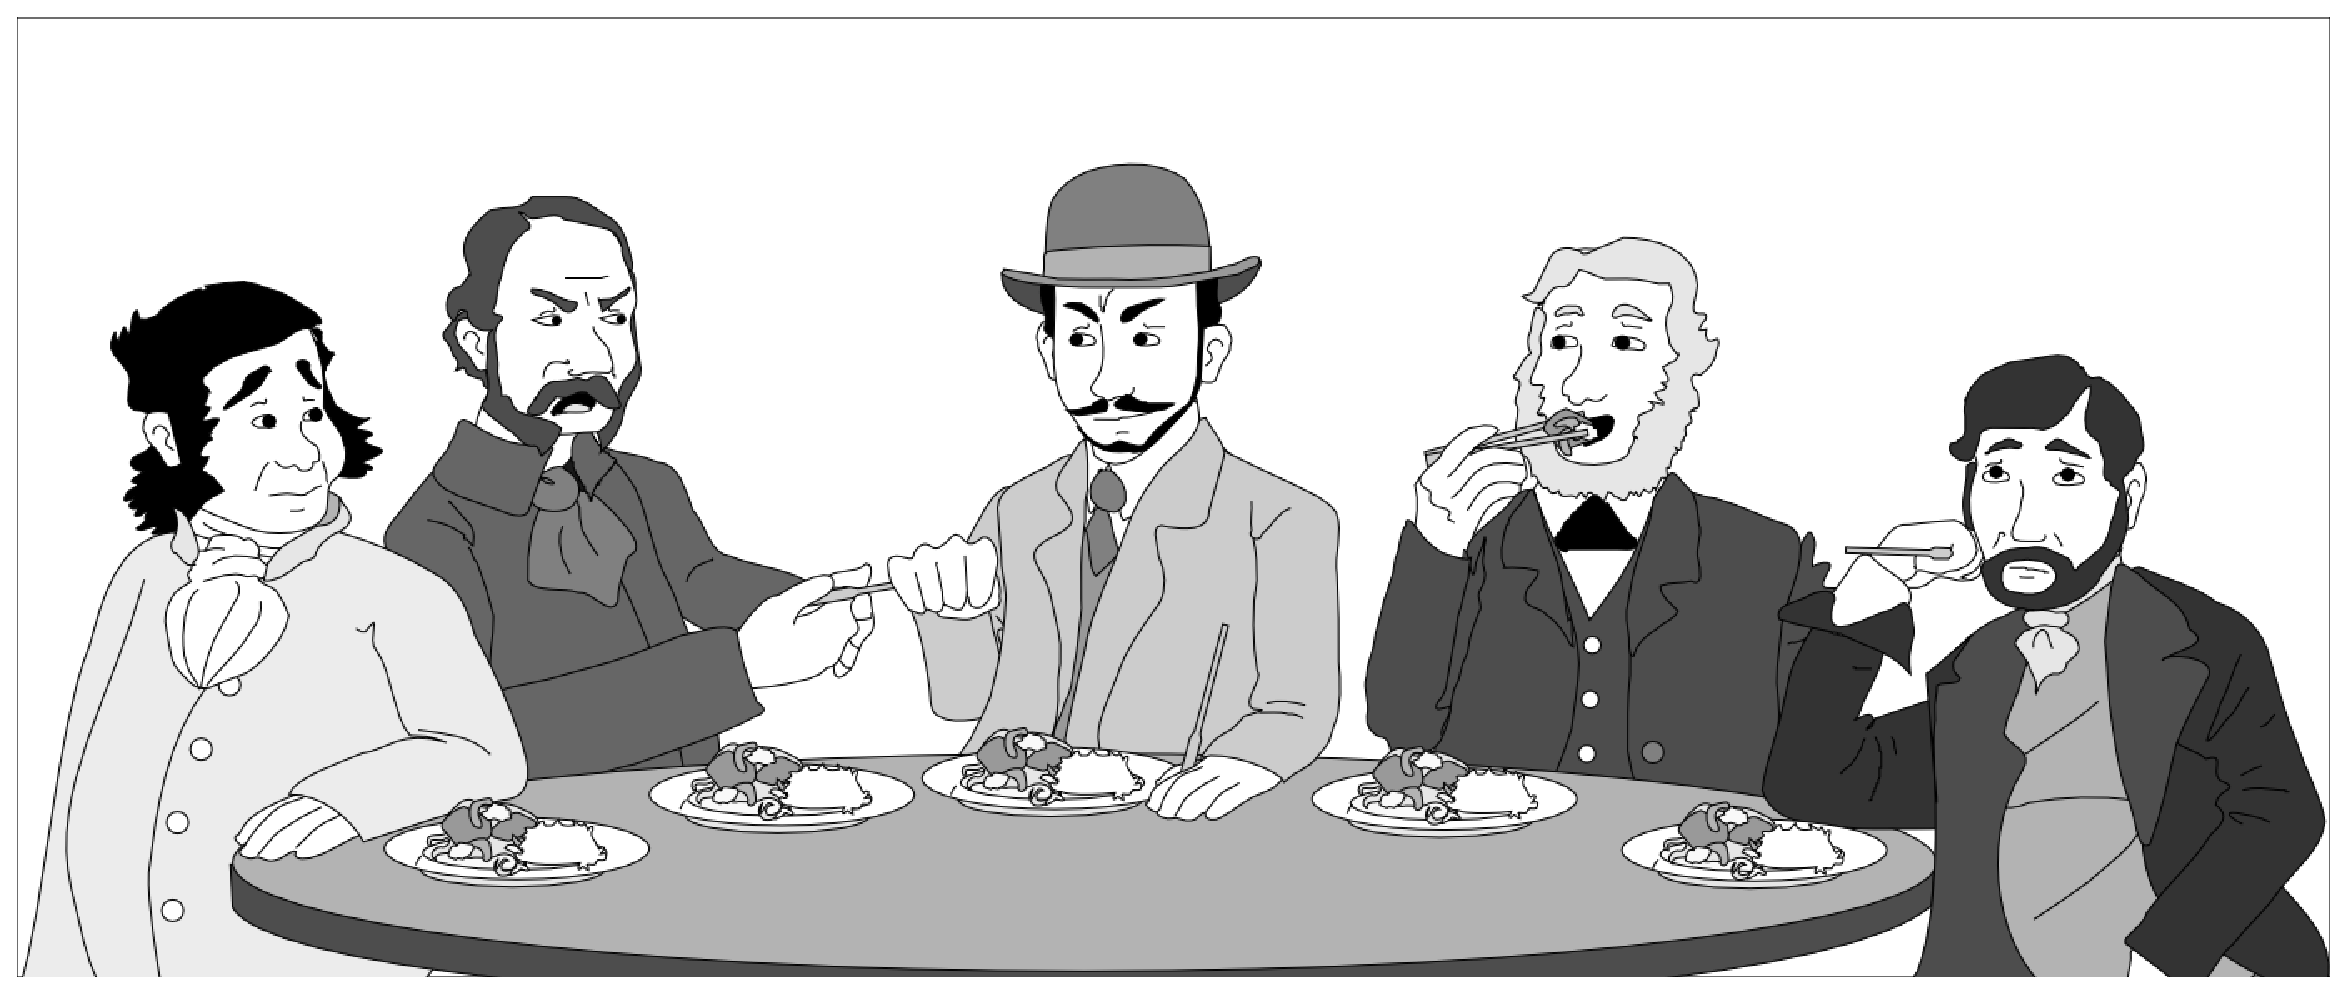
\includegraphics{cartoons/Dining-philosophers}}
\end{center}
\caption{Partial Starvation Is Also Bad}
\ContributedBy{Figure}{fig:cpu:Partial Starvation Is Also Bad}{Melissa Broussard}
\end{figure*}

The object is to construct an algorithm that, quite literally,
prevents starvation.
One starvation scenario would be if all of the philosophers picked up
their leftmost forks simultaneously.
Because none of them would put down their fork until after they ate,
and because none of them may pick up their second fork until at least
one has finished eating, they all starve.
Please note that it is not sufficient to allow at least one philosopher
to eat.
As Figure~\ref{fig:cpu:Partial Starvation Is Also Bad}
shows, starvation of even a few of the philosophers is to be avoided.

\begin{figure}[tb]
\begin{center}
\includegraphics[scale=.7]{SMPdesign/DiningPhilosopher5TB}
\end{center}
\caption{Dining Philosophers Problem, Textbook Solution}
\ContributedBy{Figure}{fig:SMPdesign:Dining Philosophers Problem, Textbook Solution}{Kornilios Kourtis}
\end{figure}

Dijkstra's solution used a global semaphore, which works fine assuming
negligible communications delays, an assumption that became invalid
in the late 1980s or early 1990s.\footnote{
	It is all too easy to denigrate Dijkstra from the viewpoint
	of the year 2012, more than 40 years after the fact.
	If you still feel the need to denigrate Dijkstra, my advice
	is to publish something, wait 40 years, and then see
	how \emph{your} words stood the test of time.}
Therefore, recent solutions number the forks as shown in
Figure~\ref{fig:SMPdesign:Dining Philosophers Problem, Textbook Solution}.
Each philosopher picks up the lowest-numbered fork next to his or her
plate, then picks up the highest-numbered fork.
The philosopher sitting in the uppermost position in the diagram thus
picks up the leftmost fork first, then the rightmost fork, while the
rest of the philosophers instead pick up their rightmost fork first.
Because two of the philosophers will attempt to pick up fork~1 first,
and because only one of those two philosophers will succeed,
there will be five forks available to four philosophers.
At least one of these four will be guaranteed to have two forks,
and thus be able to proceed eating.

This general technique of numbering resources and acquiring them in
numerical order is heavily used as a deadlock-prevention technique.
However, it is easy to imagine a sequence of events that will result
in only one philosopher eating at a time even though all are hungry:

\begin{enumerate}
    \item P2 picks up fork~1, preventing P1 from taking a fork.
    \item P3 picks up fork~2.
    \item P4 picks up fork~3.
    \item P5 picks up fork~4.
    \item P5 picks up fork~5 and eats.
    \item P5 puts down forks~4 and 5.
    \item P4 picks up fork~4 and eats.
\end{enumerate}

In short, this algorithm can result in only one philosopher eating at
a given time, even when all five philosophers are hungry,
despite the fact that there are more than enough forks for two
philosophers to eat concurrently.

Please think about ways of partitioning the Dining Philosophers Problem
before reading further.
\cleardoublepage


\begin{figure}[tb]
\begin{center}
\includegraphics[scale=.7]{SMPdesign/DiningPhilosopher4part-b}
\end{center}
\caption{Dining Philosophers Problem, Partitioned}
\ContributedBy{Figure}{fig:SMPdesign:Dining Philosophers Problem, Partitioned}{Kornilios Kourtis}
\end{figure}

One approach is shown in
Figure~\ref{fig:SMPdesign:Dining Philosophers Problem, Partitioned},
which includes four philosophers rather than five to better illustrate the
partition technique.
Here the upper and rightmost philosophers share a pair of forks,
while the lower and leftmost philosophers share another pair of forks.
If all philosophers are simultaneously hungry, at least two will
always be able to eat concurrently.
In addition, as shown in the figure, the forks can now be bundled
so that the pair are picked up and put down simultaneously, simplifying
the acquisition and release algorithms.

\QuickQuiz{}
	Is there a better solution to the Dining
	Philosophers Problem?
\QuickQuizAnswer{

\begin{figure}[tb]
\begin{center}
\includegraphics[scale=.7]{SMPdesign/DiningPhilosopher5PEM}
\end{center}
\caption{Dining Philosophers Problem, Fully Partitioned}
\QContributedBy{Figure}{fig:SMPdesign:Dining Philosophers Problem, Fully Partitioned}{Kornilios Kourtis}
\end{figure}

	One such improved solution is shown in
	Figure~\ref{fig:SMPdesign:Dining Philosophers Problem, Fully Partitioned},
	where the philosophers are simply provided with an additional
	five forks.
	All five philosophers may now eat simultaneously, and there
	is never any need for philosophers to wait on one another.
	In addition, this approach offers greatly improved disease control.

	This solution might seem like cheating to some, but such
	``cheating'' is key to finding good solutions to many
	concurrency problems.
} \QuickQuizEnd

This is an example of ``horizontal parallelism''~\cite{Inman85}
or ``data parallelism'',
so named because there is no dependency among the pairs of philosophers.
In a horizontally parallel data-processing system, a given item of data
would be processed by only one of a replicated set of software
components.

\QuickQuiz{}
	And in just what sense can this ``horizontal parallelism'' be
	said to be ``horizontal''?
\QuickQuizAnswer{
	Inman was working with protocol stacks, which are normally
	depicted vertically, with the application on top and the
	hardware interconnect on the bottom.
	Data flows up and down this stack.
	``Horizontal parallelism'' processes packets from different network
	connections in parallel, while ``vertical parallelism''
	handles different protocol-processing steps for a given
	packet in parallel.

	``Vertical parallelism'' is also called ``pipelining''.
} \QuickQuizEnd

\subsection{Double-Ended Queue}
\label{sec:SMPdesign:Double-Ended Queue}

A double-ended queue is a data structure containing a list of elements
that may be inserted or removed from either end~\cite{Knuth73}.
It has been claimed that a lock-based implementation permitting
concurrent operations on both ends of the double-ended queue is
difficult~\cite{DanGrossman2007TMGCAnalogy}.
This section shows how a partitioning design strategy can result
in a reasonably simple implementation, looking at three
general approaches in the following sections.

\subsubsection{Left- and Right-Hand Locks}
\label{sec:SMPdesign:Left- and Right-Hand Locks}

\begin{figure}[tb]
\begin{center}
\resizebox{3in}{!}{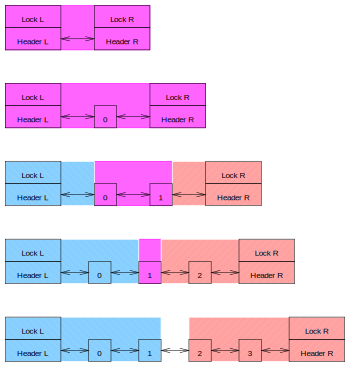
\includegraphics{SMPdesign/lockdeq}}
\end{center}
\caption{Double-Ended Queue With Left- and Right-Hand Locks}
\label{fig:SMPdesign:Double-Ended Queue With Left- and Right-Hand Locks}
\end{figure}

One seemingly straightforward approach would be to use a doubly
linked list with a left-hand lock
for left-hand-end enqueue and dequeue operations along with a right-hand
lock for right-hand-end operations, as shown in
Figure~\ref{fig:SMPdesign:Double-Ended Queue With Left- and Right-Hand Locks}.
However, the problem with this approach is that the two locks'
domains must overlap when there are fewer than four elements on the
list.
This overlap is due to the fact that removing any given element affects
not only that element, but also its left- and right-hand neighbors.
These domains are indicated by color in the figure, with blue
with downward stripes indicating
the domain of the left-hand lock, red with upward stripes
indicating the domain of the right-hand
lock, and purple (with no stripes) indicating overlapping domains.
Although it is possible to create an algorithm that works this way,
the fact that it has no fewer than five special cases should raise
a big red flag, especially given that concurrent activity at the other
end of the list can shift the queue from one special case to another
at any time.
It is far better to consider other designs.

\subsubsection{Compound Double-Ended Queue}
\label{sec:SMPdesign:Compound Double-Ended Queue}

\begin{figure}[tb]
\begin{center}
\resizebox{3in}{!}{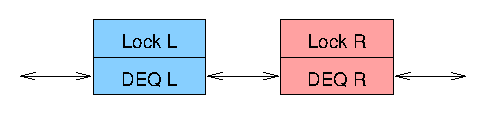
\includegraphics{SMPdesign/lockdeqpair}}
\end{center}
\caption{Compound Double-Ended Queue}
\label{fig:SMPdesign:Compound Double-Ended Queue}
\end{figure}

One way of forcing non-overlapping lock domains is shown in
Figure~\ref{fig:SMPdesign:Compound Double-Ended Queue}.
Two separate double-ended queues are run in tandem, each protected by
its own lock.
This means that elements must occasionally be shuttled from one of
the double-ended queues to the other, in which case both locks must
be held.
A simple lock hierarchy may be used to avoid deadlock, for example,
always acquiring the left-hand lock before acquiring the right-hand lock.
This will be much simpler than applying two locks to the same
double-ended queue, as we can unconditionally left-enqueue elements
to the left-hand queue and right-enqueue elements to the right-hand
queue.
The main complication arises when dequeuing from an empty queue, in
which case it is necessary to:

\begin{enumerate}
\item	If holding the right-hand lock, release it and acquire the
	left-hand lock.
\item	Acquire the right-hand lock.
\item	Rebalance the elements across the two queues.
\item	Remove the required element if there is one.
\item	Release both locks.
\end{enumerate}

\QuickQuiz{}
	In this compound double-ended queue implementation, what should
	be done if the queue has become non-empty while releasing
	and reacquiring the lock?
\QuickQuizAnswer{
	In this case, simply dequeue an item from the non-empty
	queue, release both locks, and return.
} \QuickQuizEnd

The resulting code (\co{locktdeq.c}) is quite straightforward.
The rebalancing operation might well shuttle a given element back
and forth between the two queues, wasting time and possibly requiring
workload-dependent heuristics to obtain optimal performance.
Although this might well be the best approach in some cases, it is
interesting to try for an algorithm with greater determinism.

\subsubsection{Hashed Double-Ended Queue}
\label{sec:SMPdesign:Hashed Double-Ended Queue}

One of the simplest and most effective ways to deterministically
partition a data structure is to hash it.
It is possible to trivially hash a double-ended queue by assigning
each element a sequence number based on its position in the list,
so that the first element left-enqueued into an empty queue is numbered
zero and the first element right-enqueued into an empty queue is numbered
one.
A series of elements left-enqueued into an otherwise-idle queue would
be assigned decreasing numbers (-1, -2, -3, ...), while a series of
elements right-enqueued into an otherwise-idle queue would be assigned
increasing numbers (2, 3, 4, ...).
A key point is that it is not necessary to actually represent a given
element's number, as this number will be implied by its position in
the queue.

\begin{figure}[tb]
\begin{center}
\resizebox{3in}{!}{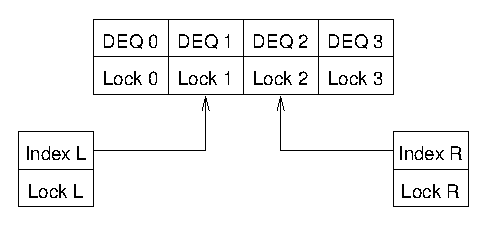
\includegraphics{SMPdesign/lockdeqhash}}
\end{center}
\caption{Hashed Double-Ended Queue}
\label{fig:SMPdesign:Hashed Double-Ended Queue}
\end{figure}

Given this approach, we assign one lock to guard the left-hand index,
one to guard the right-hand index, and one lock for each hash chain.
Figure~\ref{fig:SMPdesign:Hashed Double-Ended Queue} shows the resulting
data structure given four hash chains.
Note that the lock domains do not overlap, and that deadlock is avoided
by acquiring the index locks before the chain locks, and by never
acquiring more than one lock of each type (index or chain) at a time.

\begin{figure}[tb]
\begin{center}
\resizebox{3in}{!}{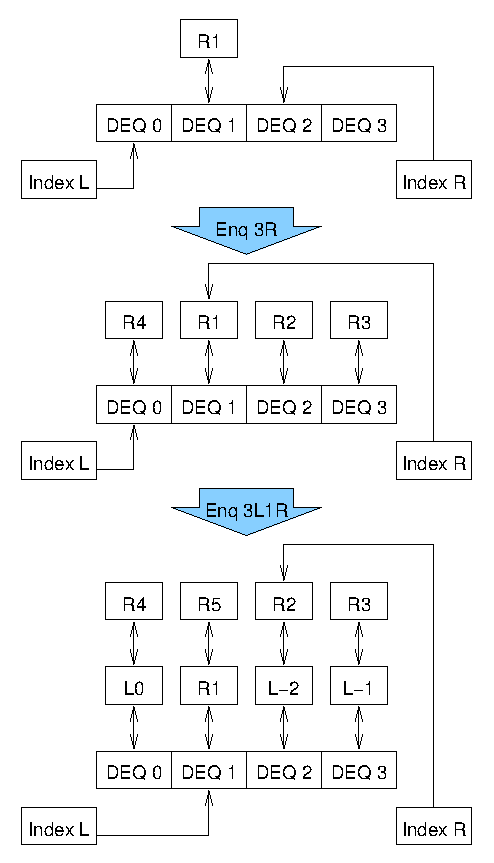
\includegraphics{SMPdesign/lockdeqhash1R}}
\end{center}
\caption{Hashed Double-Ended Queue After Insertions}
\label{fig:SMPdesign:Hashed Double-Ended Queue After Insertions}
\end{figure}

Each hash chain is itself a double-ended queue, and in this example,
each holds every fourth element.
The uppermost portion of
Figure~\ref{fig:SMPdesign:Hashed Double-Ended Queue After Insertions}
shows the state after a single element (``R1'') has been
right-enqueued, with the right-hand index having been incremented to
reference hash chain~2.
The middle portion of this same figure shows the state after
three more elements have been right-enqueued.
As you can see, the indexes are back to their initial states
(see Figure~\ref{fig:SMPdesign:Hashed Double-Ended Queue}), however,
each hash chain is now non-empty.
The lower portion of this figure shows the state after three additional
elements have been left-enqueued and an additional element has been
right-enqueued.

From the last state shown in
Figure~\ref{fig:SMPdesign:Hashed Double-Ended Queue After Insertions},
a left-dequeue operation would return element ``L-2'' and leave
the left-hand index referencing hash chain~2, which would then
contain only a single element (``R2'').
In this state, a left-enqueue running concurrently with a right-enqueue
would result in lock contention, but the probability of such contention
can be reduced to arbitrarily low levels by using a larger hash table.

\begin{figure}[tb]
\begin{center}
\resizebox{1.5in}{!}{\includegraphics{SMPdesign/lockdeqhashlots}}
\end{center}
\caption{Hashed Double-Ended Queue With 12 Elements}
\label{fig:SMPdesign:Hashed Double-Ended Queue With 12 Elements}
\end{figure}

Figure~\ref{fig:SMPdesign:Hashed Double-Ended Queue With 12 Elements}
shows how 12 elements would be organized in a four-hash-bucket
parallel double-ended queue.
Each underlying single-lock double-ended queue holds a one-quarter
slice of the full parallel double-ended queue.

\begin{figure}[tbp]
{ \scriptsize
\begin{verbatim}
  1 struct pdeq {
  2   spinlock_t llock;
  3   int lidx;
  4   spinlock_t rlock;
  5   int ridx;
  6   struct deq bkt[DEQ_N_BKTS];
  7 };
\end{verbatim}
}
\caption{Lock-Based Parallel Double-Ended Queue Data Structure}
\label{fig:SMPdesign:Lock-Based Parallel Double-Ended Queue Data Structure}
\end{figure}

Figure~\ref{fig:SMPdesign:Lock-Based Parallel Double-Ended Queue Data Structure}
shows the corresponding C-language data structure, assuming an
existing \co{struct deq} that provides a trivially locked
double-ended-queue implementation.
This data structure contains the left-hand lock on line~2,
the left-hand index on line~3, the right-hand lock on line~4
(which is cache-aligned in the actual implementation),
the right-hand index on line~5, and, finally, the hashed array
of simple lock-based double-ended queues on line~6.
A high-performance implementation would of course use padding or special
alignment directives to avoid false sharing.

\begin{figure*}[bp]
{ \scriptsize
\begin{verbatim}
  1 struct cds_list_head *pdeq_pop_l(struct pdeq *d)
  2 {
  3   struct cds_list_head *e;
  4   int i;
  5 
  6   spin_lock(&d->llock);
  7   i = moveright(d->lidx);
  8   e = deq_pop_l(&d->bkt[i]);
  9   if (e != NULL)
 10     d->lidx = i;
 11   spin_unlock(&d->llock);
 12   return e;
 13 }
 14 
 15 struct cds_list_head *pdeq_pop_r(struct pdeq *d)
 16 {
 17   struct cds_list_head *e;
 18   int i;
 19 
 20   spin_lock(&d->rlock);
 21   i = moveleft(d->ridx);
 22   e = deq_pop_r(&d->bkt[i]);
 23   if (e != NULL)
 24     d->ridx = i;
 25   spin_unlock(&d->rlock);
 26   return e;
 27 }
 28 
 29 void pdeq_push_l(struct cds_list_head *e, struct pdeq *d)
 30 {
 31   int i;
 32 
 33   spin_lock(&d->llock);
 34   i = d->lidx;
 35   deq_push_l(e, &d->bkt[i]);
 36   d->lidx = moveleft(d->lidx);
 37   spin_unlock(&d->llock);
 38 }
 39 
 40 void pdeq_push_r(struct cds_list_head *e, struct pdeq *d)
 41 {
 42   int i;
 43 
 44   spin_lock(&d->rlock);
 45   i = d->ridx;
 46   deq_push_r(e, &d->bkt[i]);
 47   d->ridx = moveright(d->ridx);
 48   spin_unlock(&d->rlock);
 49 }
\end{verbatim}
}
\caption{Lock-Based Parallel Double-Ended Queue Implementation}
\label{fig:SMPdesign:Lock-Based Parallel Double-Ended Queue Implementation}
\end{figure*}

Figure~\ref{fig:SMPdesign:Lock-Based Parallel Double-Ended Queue Implementation}
(\co{lockhdeq.c}) 
shows the implementation of the enqueue and dequeue functions.\footnote{
	One could easily create a polymorphic implementation in any
	number of languages, but doing so is left as an exercise for
	the reader.}
Discussion will focus on the left-hand operations, as the right-hand
operations are trivially derived from them.

Lines~1-13 show \co{pdeq_pop_l()}, which left-dequeues and returns
an element if possible, returning \co{NULL} otherwise.
Line~6 acquires the left-hand spinlock, and line~7 computes the
index to be dequeued from.
Line~8 dequeues the element, and, if line~9 finds the result to be
non-\co{NULL}, line~10 records the new left-hand index.
Either way, line~11 releases the lock, and, finally, line~12 returns
the element if there was one, or \co{NULL} otherwise.

Lines~29-38 shows \co{pdeq_push_l()}, which left-enqueues the specified
element.
Line~33 acquires the left-hand lock, and line~34 picks up the left-hand
index.
Line~35 left-enqueues the specified element onto the double-ended queue
indexed by the left-hand index.
Line~36 then updates the left-hand index and line~37 releases the lock.

As noted earlier, the right-hand operations are completely analogous
to their left-handed counterparts, so their analysis is left as an
exercise for the reader.

\QuickQuiz{}
	Is the hashed double-ended queue a good solution?
	Why or why not?
\QuickQuizAnswer{
	The best way to answer this is to run \url{lockhdeq.c} on
	a number of different multiprocessor systems, and you are
	encouraged to do so in the strongest possible terms.
	One reason for concern is that each operation on this
	implementation must acquire not one but two locks.
	% Getting about 500 nanoseconds per element when used as
	% a queue on a 4.2GHz Power system.  This is roughly the same as
	% the version covered by a single lock.  Sequential (unlocked
	% variant is more than an order of magnitude faster!

	The first well-designed performance study will be cited.\footnote{
		The studies by Dalessandro
		et al.~\cite{LukeDalessandro:2011:ASPLOS:HybridNOrecSTM:deque}
		and Dice et al.~\cite{DavidDice:2010:SCA:HTM:deque} are
		good starting points.}
	Do not forget to compare to a sequential implementation!
} \QuickQuizEnd

\subsubsection{Compound Double-Ended Queue Revisited}
\label{sec:SMPdesign:Compound Double-Ended Queue Revisited}

This section revisits the compound double-ended queue, using a trivial
rebalancing scheme that moves all the elements from the non-empty
queue to the now-empty queue.

\QuickQuiz{}
	Move \emph{all} the elements to the queue that became empty?
	In what possible universe is this brain-dead solution in any
	way optimal???
\QuickQuizAnswer{
	It is optimal in the case where data flow switches direction only
	rarely.
	It would of course be an extremely poor choice if the double-ended
	queue was being emptied from both ends concurrently.
	This of course raises another question, namely, in what possible
	universe emptying from both ends concurrently would be a reasonable
	thing to do.
	Work-stealing queues are one possible answer to this question.
} \QuickQuizEnd

In contrast to the hashed implementation presented in
the previous section, the compound implementation will build on
a sequential implementation of a double-ended queue that uses
neither locks nor atomic operations.

\begin{figure*}[bp]
{ \scriptsize
\begin{verbatim}
  1 struct cds_list_head *pdeq_pop_l(struct pdeq *d)
  2 {
  3   struct cds_list_head *e;
  4 
  5   spin_lock(&d->llock);
  6   e = deq_pop_l(&d->ldeq);
  7   if (e == NULL) {
  8     spin_lock(&d->rlock);
  9     e = deq_pop_l(&d->rdeq);
 10     cds_list_splice(&d->rdeq.chain, &d->ldeq.chain);
 11     CDS_INIT_LIST_HEAD(&d->rdeq.chain);
 12     spin_unlock(&d->rlock);
 13   }
 14   spin_unlock(&d->llock);
 15   return e;
 16 }
 17 
 18 struct cds_list_head *pdeq_pop_r(struct pdeq *d)
 19 {
 20   struct cds_list_head *e;
 21 
 22   spin_lock(&d->rlock);
 23   e = deq_pop_r(&d->rdeq);
 24   if (e == NULL) {
 25     spin_unlock(&d->rlock);
 26     spin_lock(&d->llock);
 27     spin_lock(&d->rlock);
 28     e = deq_pop_r(&d->rdeq);
 29     if (e == NULL) {
 30       e = deq_pop_r(&d->ldeq);
 31       cds_list_splice(&d->ldeq.chain, &d->rdeq.chain);
 32       CDS_INIT_LIST_HEAD(&d->ldeq.chain);
 33     }
 34     spin_unlock(&d->llock);
 35   }
 36   spin_unlock(&d->rlock);
 37   return e;
 38 }
 39 
 40 void pdeq_push_l(struct cds_list_head *e, struct pdeq *d)
 41 {
 42   int i;
 43 
 44   spin_lock(&d->llock);
 45   deq_push_l(e, &d->ldeq);
 46   spin_unlock(&d->llock);
 47 }
 48 
 49 void pdeq_push_r(struct cds_list_head *e, struct pdeq *d)
 50 {
 51   int i;
 52 
 53   spin_lock(&d->rlock);
 54   deq_push_r(e, &d->rdeq);
 55   spin_unlock(&d->rlock);
 56 }
\end{verbatim}
}
\caption{Compound Parallel Double-Ended Queue Implementation}
\label{fig:SMPdesign:Compound Parallel Double-Ended Queue Implementation}
\end{figure*}

Figure~\ref{fig:SMPdesign:Compound Parallel Double-Ended Queue Implementation}
shows the implementation.
Unlike the hashed implementation, this compound implementation is
asymmetric, so that we must consider the \co{pdeq_pop_l()}
and \co{pdeq_pop_r()} implementations separately.

\QuickQuiz{}
	Why can't the compound parallel double-ended queue
	implementation be symmetric?
\QuickQuizAnswer{
	The need to avoid deadlock by imposing a lock hierarchy
	forces the asymmetry, just as it does in the fork-numbering
	solution to the Dining Philosophers Problem
	(see Section~\ref{sec:SMPdesign:Dining Philosophers Problem}).
} \QuickQuizEnd

The \co{pdeq_pop_l()} implementation is shown on lines~1-16
of the figure.
Line~5 acquires the left-hand lock, which line~14 releases.
Line~6 attempts to left-dequeue an element from the left-hand underlying
double-ended queue, and, if successful, skips lines~8-13 to simply
return this element.
Otherwise, line~8 acquires the right-hand lock, line~9
left-dequeues an element from the right-hand queue,
and line~10 moves any remaining elements on the right-hand
queue to the left-hand queue, line~11 initializes the right-hand queue,
and line~12 releases the right-hand lock.
The element, if any, that was dequeued on line~10 will be returned.

The \co{pdeq_pop_r()} implementation is shown on lines~18-38
of the figure.
As before, line~22 acquires the right-hand lock (and line~36
releases it), and line~23 attempts to right-dequeue an element
from the right-hand queue, and, if successful, skips lines~24-35
to simply return this element.
However, if line~24 determines that there was no element to dequeue,
line~25 releases the right-hand lock and lines~26-27 acquire both
locks in the proper order.
Line~28 then attempts to right-dequeue an element from the right-hand
list again, and if line~29 determines that this second attempt has
failed, line~30 right-dequeues an element from the left-hand queue
(if there is one available), line~31 moves any remaining elements
from the left-hand queue to the right-hand queue, and line~32
initializes the left-hand queue.
Either way, line~34 releases the left-hand lock.

\QuickQuiz{}
	Why is it necessary to retry the right-dequeue operation
	on line~28 of
	Figure~\ref{fig:SMPdesign:Compound Parallel Double-Ended Queue Implementation}?
\QuickQuizAnswer{
	This retry is necessary because some other thread might have
	enqueued an element between the time that this thread dropped
	\co{d->rlock} on line~25 and the time that it reacquired this
	same lock on line~27.
} \QuickQuizEnd

\QuickQuiz{}
	Surely the left-hand lock must \emph{sometimes} be available!!!
	So why is it necessary that line~25 of
	Figure~\ref{fig:SMPdesign:Compound Parallel Double-Ended Queue Implementation}
	unconditionally release the right-hand lock?
\QuickQuizAnswer{
	It would be possible to use \co{spin_trylock()} to attempt
	to acquire the left-hand lock when it was available.
	However, the failure case would still need to drop the
	right-hand lock and then re-acquire the two locks in order.
	Making this transformation (and determining whether or not
	it is worthwhile) is left as an exercise for the reader.
} \QuickQuizEnd

The \co{pdeq_push_l()} implementation is shown on lines~40-47 of
Figure~\ref{fig:SMPdesign:Compound Parallel Double-Ended Queue Implementation}.
Line~44 acquires the left-hand spinlock, line~45 left-enqueues the
element onto the left-hand queue, and finally line~46 releases
the lock.
The \co{pdeq_enqueue_r()} implementation (shown on lines~49-56)
is quite similar.

\subsubsection{Double-Ended Queue Discussion}
\label{sec:SMPdesign:Double-Ended Queue Discussion}

The compound implementation is somewhat more complex than the
hashed variant presented in
Section~\ref{sec:SMPdesign:Hashed Double-Ended Queue},
but is still reasonably simple.
Of course, a more intelligent rebalancing scheme could be arbitrarily
complex, but the simple scheme shown here has been shown to
perform well compared to software
alternatives~\cite{LukeDalessandro:2011:ASPLOS:HybridNOrecSTM:deque}
and even compared to algorithms using hardware
assist~\cite{DavidDice:2010:SCA:HTM:deque}.
Nevertheless, the best we can hope for from such a scheme
is 2x scalability, as at most two threads can be holding the
dequeue's locks concurrently.
This limitation also applies to algorithms based on non-blocking
synchronization, such as the compare-and-swap-based dequeue algorithm of
Michael~\cite{DBLP:conf/europar/Michael03}.\footnote{
	This paper is interesting in that it showed that special
	double-compare-and-swap (DCAS) instructions are not needed
	for lock-free implementations of double-ended queues.
	Instead, the common compare-and-swap (e.g., x86 cmpxchg)
	suffices.}

\QuickQuiz{}
	Why are there not one but two solutions to the double-ended queue
	problem?
\QuickQuizAnswer{
	There are actually at least three.
	The third, by Dominik Dingel, makes interesting use of
	reader-writer locking, and may be found in \co{lockrwdeq.c}.
} \QuickQuizEnd

In fact, as noted by Dice et al.~\cite{DavidDice:2010:SCA:HTM:deque},
an unsynchronized single-threaded double-ended queue significantly
outperforms any of the parallel implementations they studied.
Therefore, the key point is that there can be significant overhead enqueuing to
or dequeuing from a shared queue, regardless of implementation.
This should come as no surprise given the material in
Chapter~\ref{chp:Hardware and its Habits}, given the strict
FIFO nature of these queues.

Furthermore, these strict FIFO queues are strictly FIFO only with
respect to
\emph{linearization points}~\cite{Herlihy:1990:LCC:78969.78972}\footnote{
	In short, a linearization point is a single point within a given
	function where that function can be said to have taken effect.
	In this lock-based implementation, the linearization points
	can be said to be anywhere within the critical section that
	does the work.}
that are not visible to the caller, in fact, in these examples,
the linearization points are buried in the lock-based critical
sections.
These queues are not strictly FIFO with respect to (say) the times at which
the individual operations started~\cite{AndreasHaas2012FIFOisnt}.
This indicates that the strict FIFO property is not all that valuable
in concurrent programs, and in fact, Kirsch et al.~present less-strict
queues that provide improved performance and
scalability~\cite{ChristophMKirsch2012FIFOisntTR}.\footnote{
	Nir Shavit produced relaxed stacks for roughly the same
	reasons~\cite{Shavit:2011:DSM:1897852.1897873}.
	This situation leads some to believe that the linearization
	points are useful to theorists rather than developers, and
	leads others to wonder to what extent the designers of such
	data structures and algorithms were considering the needs
	of their users.}
All that said, if you are pushing all the data used by your concurrent
program through a single queue, you really need to rethink your
overall design.

\subsection{Partitioning Example Discussion}
\label{sec:SMPdesign:Partitioning Example Discussion}

The optimal solution to the dining philosophers problem given in
the answer to the Quick Quiz in
Section~\ref{sec:SMPdesign:Dining Philosophers Problem}
is an excellent example of ``horizontal parallelism'' or
``data parallelism''.
The synchronization overhead in this case is nearly (or even exactly)
zero.
In contrast, the double-ended
queue implementations are examples of ``vertical parallelism'' or
``pipelining'', given that data moves from one thread to another.
The tighter coordination required for pipelining in turn requires
larger units of work to obtain a given level of efficiency.

\QuickQuiz{}
	The tandem double-ended queue runs about twice as fast as
	the hashed double-ended queue, even when I increase the
	size of the hash table to an insanely large number.
	Why is that?
\QuickQuizAnswer{
	The hashed double-ended queue's locking design only permits
	one thread at a time at each end, and further requires
	two lock acquisitions for each operation.
	The tandem double-ended queue also permits one thread at a time
	at each end, and in the common case requires only one lock
	acquisition per operation.
	Therefore, the tandem double-ended queue should be expected to
	outperform the hashed double-ended queue.

	Can you created a double-ended queue that allows multiple
	concurrent operations at each end?
	If so, how?  If not, why not?
} \QuickQuizEnd

\QuickQuiz{}
	Is there a significantly better way of handling concurrency
	for double-ended queues?
\QuickQuizAnswer{
	One approach is to transform the problem to be solved
	so that multiple double-ended queues can be used in parallel,
	allowing the simpler single-lock double-ended queue to be used,
	and perhaps also replace each double-ended queue with a pair of
	conventional single-ended queues.
	Without such ``horizontal scaling'', the speedup is limited
	to 2.0.
	In contrast, horizontal-scaling designs can achieve very large
	speedups, and are especially attractive if there are multiple threads
	working either end of the queue, because in this
	multiple-thread case the dequeue
	simply cannot provide strong ordering guarantees.
	After all, the fact that a given thread removed an item first
	in no way implies that it will process that item
	first~\cite{AndreasHaas2012FIFOisnt}.
	And if there are no guarantees, we may as well obtain the
	performance benefits that come with refusing to provide these
	guarantees.
	% about twice as fast as hashed version on 4.2GHz Power.

	Regardless of whether or not the problem can be transformed
	to use multiple queues, it is worth asking whether work can
	be batched so that each enqueue and dequeue operation corresponds
	to larger units of work.
	This batching approach decreases contention on the queue data
	structures, which increases both performance and scalability,
	as will be seen in
	Section~\ref{sec:SMPdesign:Synchronization Granularity}.
	After all, if you must incur high synchronization overheads,
	be sure you are getting your money's worth.

	Other researchers are working on other ways to take advantage
	of limited ordering guarantees in
	queues~\cite{ChristophMKirsch2012FIFOisntTR}.
} \QuickQuizEnd

These two examples show just how powerful partitioning can be in
devising parallel algorithms.
Section~\ref{sec:SMPdesign:Locking Granularity and Performance}
looks briefly at a third example, matrix multiply.
However, all three of these examples beg for more and better design
criteria for parallel programs, a topic taken up in the next section.


% SMPdesign/criteria.tex
% mainfile: ../perfbook.tex
% SPDX-License-Identifier: CC-BY-SA-3.0

\section{Design Criteria}
\label{sec:SMPdesign:Design Criteria}
%
\epigraph{One pound of learning requires ten pounds of commonsense to apply it.}
	 {Persian proverb}

One way to obtain the best performance and scalability is to simply
hack away until you converge on the best possible parallel program.
Unfortunately, if your program is other than microscopically tiny,
the space of possible parallel programs is so huge
that convergence is not guaranteed in the lifetime of the universe.
Besides, what exactly is the ``best possible parallel program''?
After all, \cref{sec:intro:Parallel Programming Goals}
called out no fewer than three parallel-programming goals of
\IX{performance}, \IX{productivity}, and \IX{generality},
and the best possible performance will likely come at a cost in
terms of productivity and generality.
We clearly need to be able to make higher-level choices at design
time in order to arrive at an acceptably good parallel program
before that program becomes obsolete.

However, more detailed design criteria are required to
actually produce a real-world design, a task taken up in this section.
This being the real world, these criteria often conflict to a
greater or lesser degree, requiring that the designer carefully
balance the resulting tradeoffs.

As such, these criteria may be thought of as the ``forces''
acting on the design, with particularly good tradeoffs between
these forces being called ``design patterns''~\cite{Alexander79,GOF95}.

The design criteria for attaining the three parallel-programming goals
are speedup,
contention, overhead, read-to-write ratio, and complexity:
\begin{description}
\item[Speedup:]  As noted in
	\cref{sec:intro:Parallel Programming Goals},
	increased performance is the major reason
	to go to all of the time and trouble
	required to parallelize it.
	Speedup is defined to be the ratio of the time required
	to run a sequential version of the program to the time
	required to run a parallel version.
\item[Contention:]  If more CPUs are applied to a parallel
	program than can be kept busy by that program,
	the excess CPUs are prevented from doing
	useful work by contention.
	This may be \IX{lock contention}, memory contention, or a host
	of other performance killers.
\item[Work-to-Synchronization Ratio:]  A uniprocessor,
	single\-/threaded, non-preemptible, and non\-/interruptible\footnote{
		Either by masking interrupts or by being oblivious to them.}
	version of a given parallel
	program would not need any synchronization primitives.
	Therefore, any time consumed by these primitives
	(including communication cache misses as well as
	\IXh{message}{latency}, locking primitives, atomic instructions,
	and \IXpl{memory barrier})
	is overhead that does not contribute directly to the useful
	work that the program is intended to accomplish.
	Note that the important measure is the
	relationship between the synchronization overhead
	and the overhead of the code in the \IX{critical section}, with larger
	critical sections able to tolerate greater synchronization overhead.
	The work-to-synchronization ratio is related to
	the notion of synchronization efficiency.
\item[Read-to-Write Ratio:]  A data structure that is
	rarely updated may often be replicated rather than partitioned,
	and furthermore may be protected with asymmetric
	synchronization primitives that reduce readers' synchronization
	overhead at the expense of that of writers, thereby
	reducing overall synchronization overhead.
	Corresponding optimizations are possible for frequently
	updated data structures, as discussed in
	\cref{chp:Counting}.
\item[Complexity:]  A parallel program is more complex than
	an equivalent sequential program because the parallel program
	has a much larger state space than does the sequential program,
	although large state spaces having regular structures can in
	some cases be easily understood.
	A parallel programmer must
	consider synchronization primitives, messaging, locking design,
	critical-section identification,
	and deadlock in the context of this larger state space.

	This greater complexity often translates
	to higher development and maintenance costs.
	Therefore, budgetary constraints can
	limit the number and types of modifications made to
	an existing program, since a given degree of speedup is
	worth only so much time and trouble.
	Worse yet, added complexity can actually \emph{reduce}
	performance and scalability.

	Therefore, beyond a certain point,
	there may be potential sequential optimizations
	that are cheaper and more effective than parallelization.
	As noted in
	\cref{sec:intro:Performance},
	parallelization is but one performance optimization of
	many, and is furthermore an optimization that applies
	most readily to CPU-based bottlenecks.
\end{description}
These criteria will act together to enforce a maximum speedup.
The first three criteria are deeply interrelated, so
the remainder of this section analyzes these
interrelationships.\footnote{
	A real-world parallel system will be subject to many additional
	design criteria, such as data-structure layout,
	memory size, memory-hierarchy latencies, bandwidth limitations,
	and I/O issues.}

Note that these criteria may also appear as part of the requirements
specification, and further that they are one solution to the problem
of summarizing the quality of a concurrent algorithm from
\cpageref{sec:SMPdesign:Problems Quality Assessment}.
For example, speedup may act as a relative desideratum
(``the faster, the better'')
or as an absolute requirement of the workload (``the system
must support at least 1,000,000 web hits per second'').
Classic design pattern languages describe relative desiderata as forces
and absolute requirements as context.

An understanding of the relationships between these design criteria can
be very helpful when identifying appropriate design tradeoffs for a
parallel program.
\begin{enumerate}
\item	The less time a program spends in exclusive-lock critical sections,
	the greater the potential speedup.
	This is a consequence of \IXr{Amdahl's Law}~\cite{GeneAmdahl1967AmdahlsLaw}
	because only one CPU may execute within a given
	exclusive-lock critical section at a given time.

	More specifically, for unbounded linear scalability, the fraction
	of time that the program spends in a given exclusive critical
	section must decrease as the number of CPUs increases.
	For example, a program will not scale to 10~CPUs
	unless it spends much less than one tenth of its time in the
	most-restrictive exclusive-lock critical section.
\item	Contention effects consume the excess CPU and/or
	wallclock time when the actual speedup is less than
	the number of available CPUs.
	The larger the gap between the number of CPUs
	and the actual speedup, the less efficiently the
	CPUs will be used.
	Similarly, the greater the desired efficiency, the smaller
	the achievable speedup.
\item	If the available synchronization primitives have
	high overhead compared to the critical sections
	that they guard, the best way to improve speedup
	is to reduce the number of times that the primitives
	are invoked.
	This can be accomplished by batching critical sections,
	using data ownership (see \cref{chp:Data Ownership}),
	using asymmetric primitives
	(see \cref{chp:Deferred Processing}),
	or by using a coarse-grained design such as \IXh{code}{locking}.
\item	If the critical sections have high overhead compared
	to the primitives guarding them, the best way
	to improve speedup is to increase parallelism
	by moving to reader/writer locking, \IXh{data}{locking}, asymmetric,
	or data ownership.
\item	If the critical sections have high overhead compared
	to the primitives guarding them and the data structure
	being guarded is read much more often than modified,
	the best way to increase parallelism is to move
	to reader/writer locking or asymmetric primitives.
\item	Many changes that improve SMP performance, for example,
	reducing lock contention, also improve real-time
	latencies~\cite{PaulMcKenney2005h}.
\end{enumerate}

\QuickQuiz{
	Don't all these problems with critical sections mean that
	we should just always use
	non-blocking synchronization~\cite{MauriceHerlihy90a},
	which don't have critical sections?
}\QuickQuizAnswer{
	Although non-blocking synchronization can be very useful
	in some situations, it is no panacea, as discussed in
	\cref{sec:advsync:Non-Blocking Synchronization}.
	Also, non-blocking synchronization really does have
	critical sections, as noted by Josh Triplett.
	For example, in a non-blocking algorithm based on
	compare-and-swap operations, the code starting at the
	initial load and continuing to the compare-and-swap
	is analogous to a lock-based critical section.
}\QuickQuizEnd

It is worth reiterating that contention has many guises, including
lock contention, memory contention, cache overflow, \IX{thermal throttling},
and much else besides.
This chapter looks primarily at lock and memory contention.


\section{Synchronization Granularity}
\label{sec:SMPdesign:Synchronization Granularity}

\begin{figure}[tb]
\begin{center}
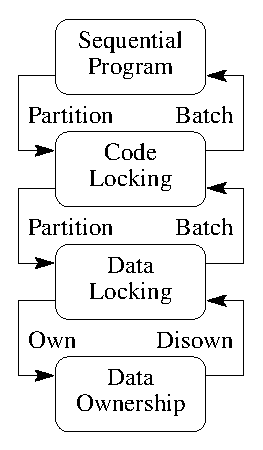
\includegraphics{SMPdesign/LockGranularity}
\end{center}
\caption{Design Patterns and Lock Granularity}
\label{fig:SMPdesign:Design Patterns and Lock Granularity}
\end{figure}

Figure~\ref{fig:SMPdesign:Design Patterns and Lock Granularity}
gives a pictorial view of different levels of synchronization granularity,
each of which is described in one of the following sections.
These sections focus primarily on locking, but similar granularity
issues arise with all forms of synchronization.

\subsection{Sequential Program}
\label{sec:SMPdesign:Sequential Program}

If the program runs fast enough on a single processor, and
has no interactions with other processes, threads, or interrupt
handlers, you should
remove the synchronization primitives and spare yourself their
overhead and complexity.
Some years back, there were those who would argue that Moore's Law
would eventually force all programs into this category.
However,
% @@@ Intel Trademark
as can be seen in
Figure~\ref{fig:SMPdesign:Clock-Frequency Trend for Intel CPUs},
the exponential increase in single-threaded performance halted in
about 2003.
Therefore,
increasing performance will increasingly require parallelism.\footnote{
	This plot shows clock frequencies for newer CPUs theoretically
	capable of retiring one or more instructions per clock, and MIPS for
	older CPUs requiring multiple clocks to execute even the
	simplest instruction.
	The reason for taking this approach is that the newer CPUs'
	ability to retire multiple instructions per clock is typically
	limited by memory-system performance.}
The debate as to whether this new trend will result in single chips
with thousands
of CPUs will not be settled soon, but given that Paul is typing this
sentence on a dual-core laptop, the age of SMP does seem to be upon us.
It is also important to note that Ethernet bandwidth is continuing
to grow, as shown in
Figure~\ref{fig:SMPdesign:Ethernet Bandwidth vs. Intel x86 CPU Performance}.
This growth will motivate multithreaded servers in order to handle
the communications load.

\begin{figure}[htb]
\begin{center}
\resizebox{3in}{!}{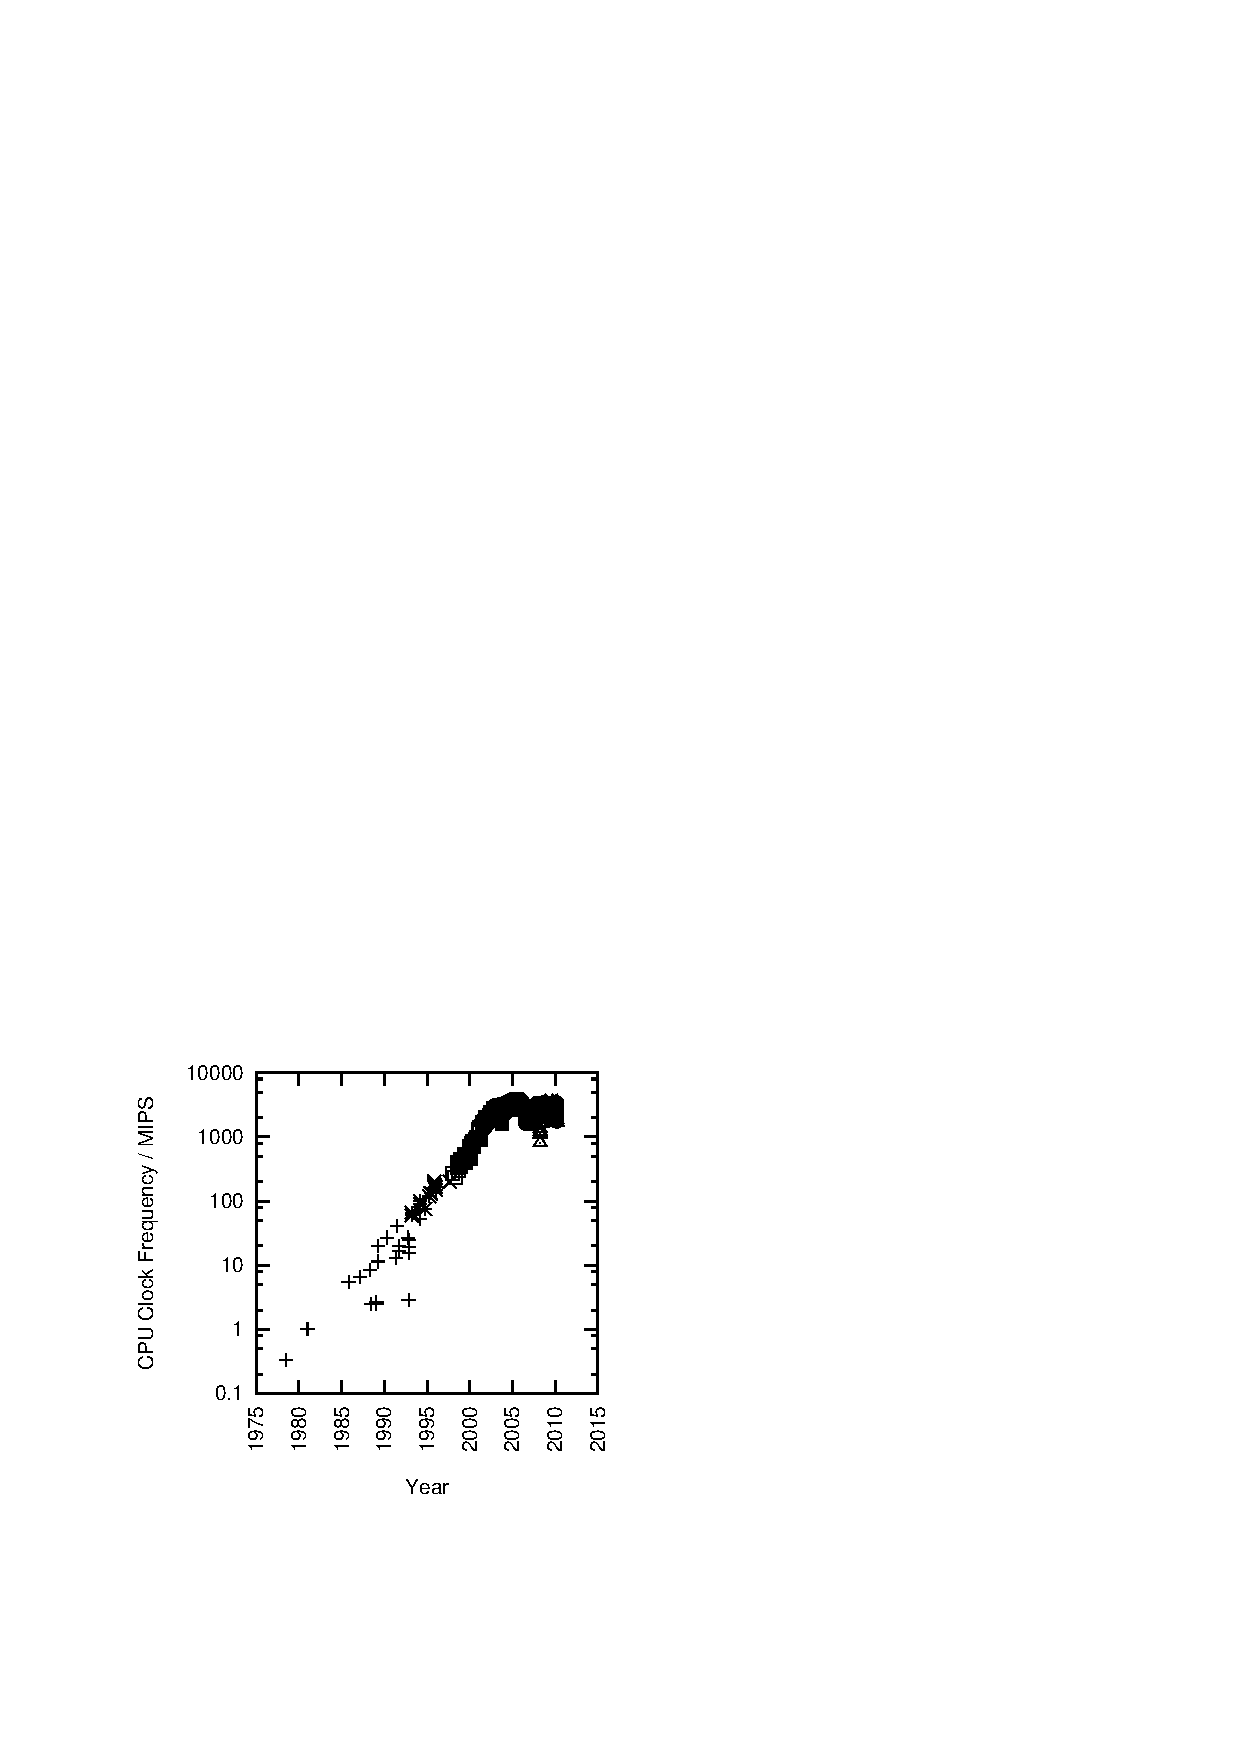
\includegraphics{SMPdesign/clockfreq}}
\end{center}
\caption{MIPS/Clock-Frequency Trend for Intel CPUs}
\label{fig:SMPdesign:Clock-Frequency Trend for Intel CPUs}
\end{figure}

\begin{figure}[htb]
\begin{center}
\resizebox{3in}{!}{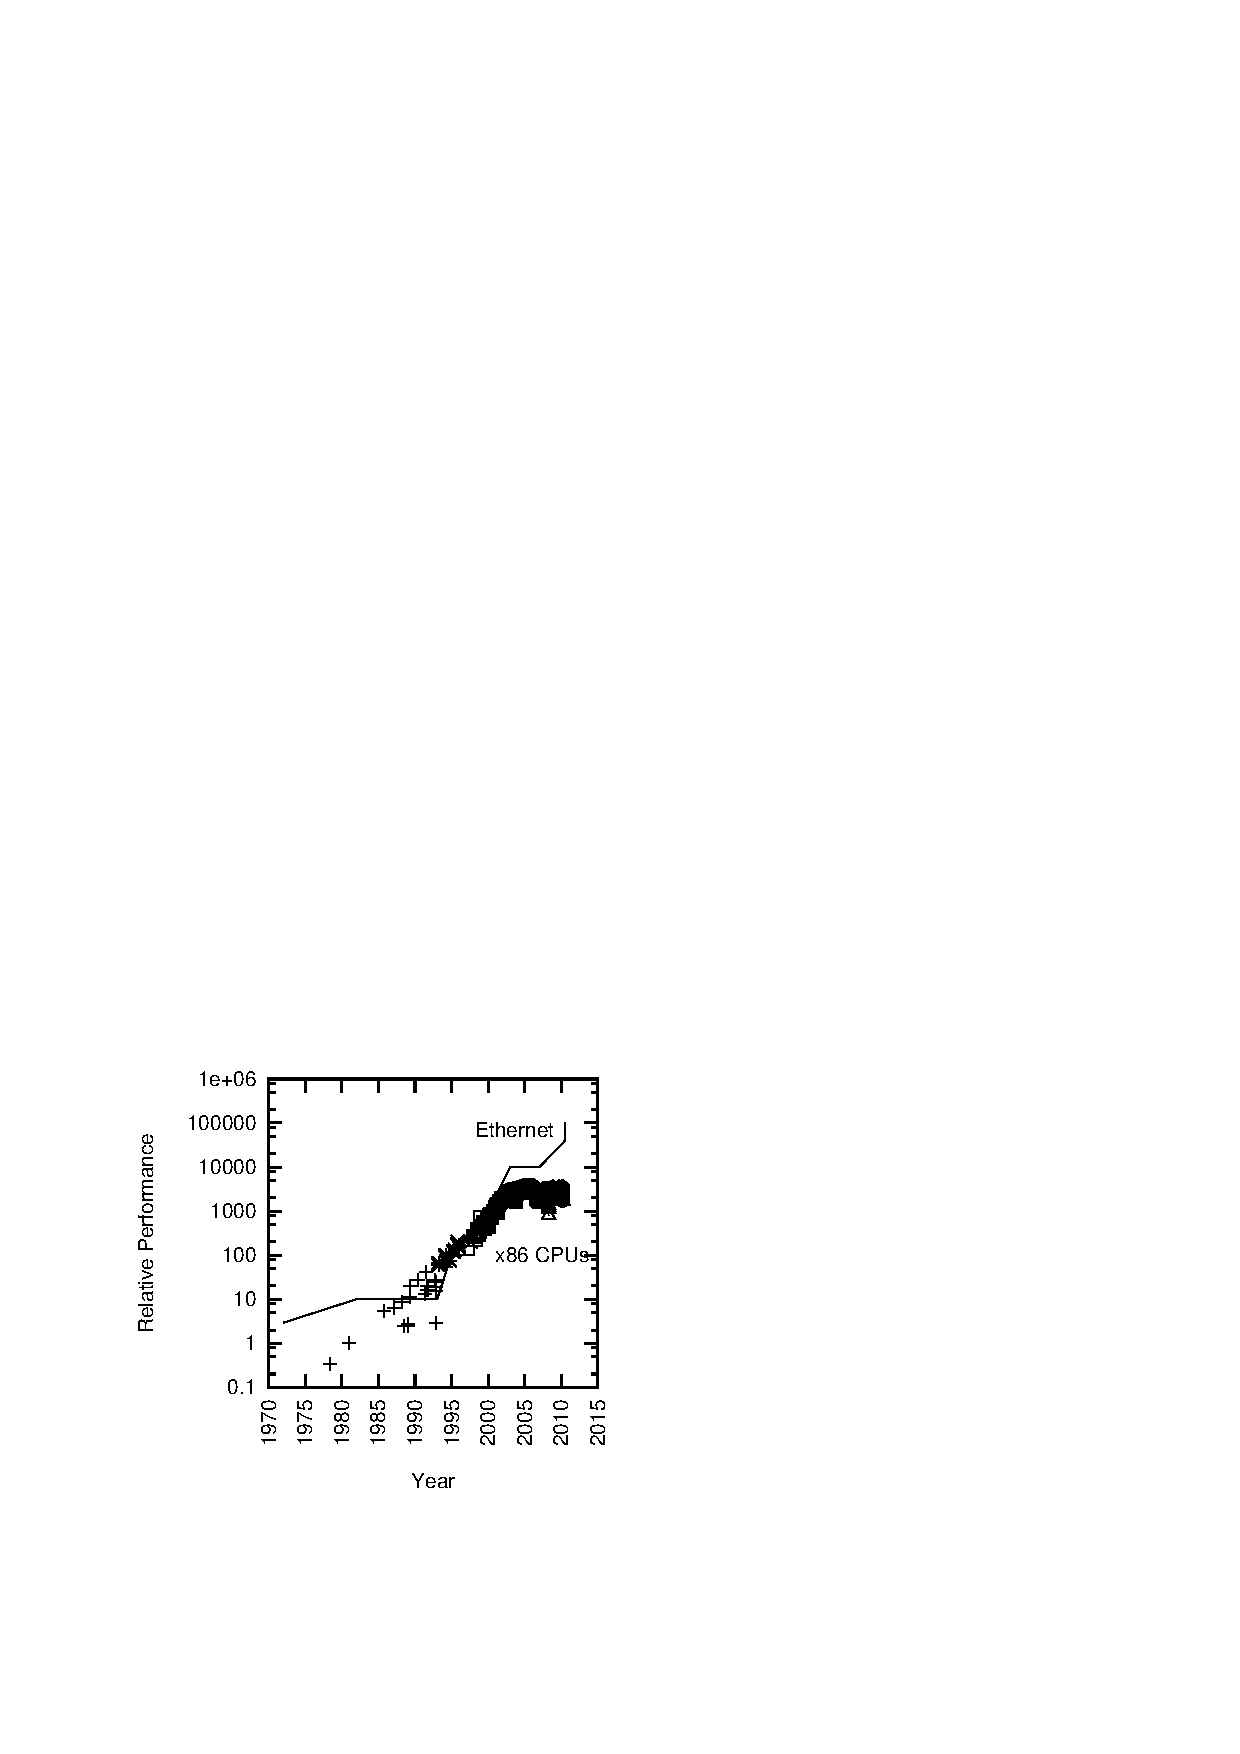
\includegraphics{SMPdesign/CPUvsEnet}}
\end{center}
\caption{Ethernet Bandwidth vs. Intel x86 CPU Performance}
\label{fig:SMPdesign:Ethernet Bandwidth vs. Intel x86 CPU Performance}
\end{figure}

Please note that this does \emph{not} mean that you should code each
and every program in a multi-threaded manner.
Again, if a program runs quickly enough on a single processor,
spare yourself the overhead and complexity of SMP synchronization
primitives.
The simplicity of the hash-table lookup code in
Figure~\ref{fig:SMPdesign:Sequential-Program Hash Table Search}
underscores this point.\footnote{
	The examples in this section are taken from Hart et
	al.~\cite{ThomasEHart2006a}, adapted for clarity
	by gathering related code from multiple files.}
A key point is that speedups due to parallelism are normally
limited to the number of CPUs.
In contrast, speedups due to sequential optimizations, for example,
careful choice of data structure, can be arbitrarily large.

\begin{figure}[htbp]
{ \scriptsize
\begin{verbatim}
  1 struct hash_table
  2 {
  3   long nbuckets;
  4   struct node **buckets;
  5 };
  6
  7 typedef struct node {
  8   unsigned long key;
  9   struct node *next;
 10 } node_t;
 11
 12 int hash_search(struct hash_table *h, long key)
 13 {
 14   struct node *cur;
 15
 16   cur = h->buckets[key % h->nbuckets];
 17   while (cur != NULL) {
 18     if (cur->key >= key) {
 19       return (cur->key == key);
 20     }
 21     cur = cur->next;
 22   }
 23   return 0;
 24 }
\end{verbatim}
}
\caption{Sequential-Program Hash Table Search}
\label{fig:SMPdesign:Sequential-Program Hash Table Search}
\end{figure}

% ./test_hash_null.exe 1000 0/100 1 1024 1
% ./test_hash_null.exe: nmilli: 1000 update/total: 0/100 nelements: 1 nbuckets: 1024 nthreads: 1
% ./test_hash_null.exe: avg = 96.2913  max = 98.2337  min = 90.4095  std = 2.95314
% ./test_hash_null.exe: nmilli: 1000 update/total: 0/100 nelements: 1 nbuckets: 1024 nthreads: 1
% ./test_hash_null.exe: avg = 91.5592  max = 97.3315  min = 89.9885  std = 2.88925
% ./test_hash_null.exe: nmilli: 1000 update/total: 0/100 nelements: 1 nbuckets: 1024 nthreads: 1
% ./test_hash_null.exe: avg = 93.3568  max = 106.162  min = 89.8828  std = 6.40418

On the other hand, if you are not in this happy situation, read on!

\subsection{Code Locking}
\label{sec:SMPdesign:Code Locking}

Code locking is quite simple due to the fact that is uses only
global locks.\footnote{
	If your program instead has locks in data structures,
	or, in the case of Java, uses classes with synchronized
	instances, you are instead using ``data locking'', described
	in Section~\ref{sec:SMPdesign:Data Locking}.}
It is especially
easy to retrofit an existing program to use code locking in
order to run it on a multiprocessor.  If the program has
only a single shared resource, code locking will even give
optimal performance.
However, many of the larger and more complex programs
require much of the execution to
occur in critical sections, which in turn causes code locking
to sharply limits their scalability.

Therefore, you should use code locking on programs that spend
only a small fraction of their execution time in critical sections or
from which only modest scaling is required.  In these cases,
code locking will provide a relatively simple program that is
very similar to its sequential counterpart,
as can be seen in
Figure~\ref{fig:SMPdesign:Code-Locking Hash Table Search}.
However, note that the simple return of the comparison in
\co{hash_search()} in
Figure~\ref{fig:SMPdesign:Sequential-Program Hash Table Search}
has now become three statements due to the need to release the
lock before returning.

\begin{figure}[htbp]
{ \scriptsize
\begin{verbatim}
  1 spinlock_t hash_lock;
  2
  3 struct hash_table
  4 {
  5   long nbuckets;
  6   struct node **buckets;
  7 };
  8
  9 typedef struct node {
 10   unsigned long key;
 11   struct node *next;
 12 } node_t;
 13
 14 int hash_search(struct hash_table *h, long key)
 15 {
 16   struct node *cur;
 17   int retval;
 18
 19   spin_lock(&hash_lock);
 20   cur = h->buckets[key % h->nbuckets];
 21   while (cur != NULL) {
 22     if (cur->key >= key) {
 23       retval = (cur->key == key);
 24       spin_unlock(&hash_lock);
 25       return retval;
 26     }
 27     cur = cur->next;
 28   }
 29   spin_unlock(&hash_lock);
 30   return 0;
 31 }
\end{verbatim}
}
\caption{Code-Locking Hash Table Search}
\label{fig:SMPdesign:Code-Locking Hash Table Search}
\end{figure}

Unfortunately, code locking is particularly prone to ``lock contention'',
where multiple CPUs need to acquire the lock concurrently.
SMP programmers who have taken care of groups of small children
(or groups of older people who are acting like children) will immediately
recognize the danger of having only one of something,
as illustrated in Figure~\ref{fig:SMPdesign:Lock Contention}.

% ./test_hash_codelock.exe 1000 0/100 1 1024 1
% ./test_hash_codelock.exe: nmilli: 1000 update/total: 0/100 nelements: 1 nbuckets: 1024 nthreads: 1
% ./test_hash_codelock.exe: avg = 164.115  max = 170.388  min = 161.659  std = 3.21857
% ./test_hash_codelock.exe: nmilli: 1000 update/total: 0/100 nelements: 1 nbuckets: 1024 nthreads: 1
% ./test_hash_codelock.exe: avg = 181.17  max = 198.4  min = 162.459  std = 15.8585
% ./test_hash_codelock.exe: nmilli: 1000 update/total: 0/100 nelements: 1 nbuckets: 1024 nthreads: 1
% ./test_hash_codelock.exe: avg = 167.651  max = 189.014  min = 162.144  std = 10.6819

% ./test_hash_codelock.exe 1000 0/100 1 1024 2
% ./test_hash_codelock.exe: nmilli: 1000 update/total: 0/100 nelements: 1 nbuckets: 1024 nthreads: 2
% ./test_hash_codelock.exe: avg = 378.481  max = 385.971  min = 374.235  std = 4.05934
% ./test_hash_codelock.exe: nmilli: 1000 update/total: 0/100 nelements: 1 nbuckets: 1024 nthreads: 2
% ./test_hash_codelock.exe: avg = 753.414  max = 1015.28  min = 377.734  std = 294.942
% ./test_hash_codelock.exe: nmilli: 1000 update/total: 0/100 nelements: 1 nbuckets: 1024 nthreads: 2
% ./test_hash_codelock.exe: avg = 502.737  max = 980.924  min = 374.406  std = 239.383

One solution to this problem, named ``data locking'', is described
in the next section.

\begin{figure}[htb]
\begin{center}
\resizebox{3in}{!}{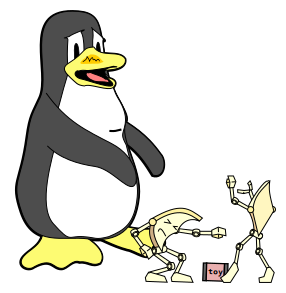
\includegraphics{cartoons/r-2014-Data-one-fighting}}
\end{center}
\caption{Lock Contention}
\ContributedBy{Figure}{fig:SMPdesign:Lock Contention}{Melissa Broussard}
\end{figure}

\subsection{Data Locking}
\label{sec:SMPdesign:Data Locking}

Many data structures may be partitioned,
with each partition of the data structure having its own lock.
Then the critical sections for each part of the data structure
can execute in parallel,
although only one instance of the critical section for a given
part could be executing at a given time.
You should use data locking when contention must
be reduced, and where synchronization overhead is not
limiting speedups.
Data locking reduces contention by distributing the instances
of the overly-large critical section across multiple data structures,
for example, maintaining per-hash-bucket critical sections in a
hash table, as shown in
Figure~\ref{fig:SMPdesign:Data-Locking Hash Table Search}.
The increased scalability again results in a slight increase in complexity
in the form of an additional data structure, the \co{struct bucket}.

\begin{figure}[htbp]
{ \scriptsize
\begin{verbatim}
  1 struct hash_table
  2 {
  3   long nbuckets;
  4   struct bucket **buckets;
  5 };
  6
  7 struct bucket {
  8   spinlock_t bucket_lock;
  9   node_t *list_head;
 10 };
 11
 12 typedef struct node {
 13   unsigned long key;
 14   struct node *next;
 15 } node_t;
 16
 17 int hash_search(struct hash_table *h, long key)
 18 {
 19   struct bucket *bp;
 20   struct node *cur;
 21   int retval;
 22
 23   bp = h->buckets[key % h->nbuckets];
 24   spin_lock(&bp->bucket_lock);
 25   cur = bp->list_head;
 26   while (cur != NULL) {
 27     if (cur->key >= key) {
 28       retval = (cur->key == key);
 29       spin_unlock(&bp->bucket_lock);
 30       return retval;
 31     }
 32     cur = cur->next;
 33   }
 34   spin_unlock(&bp->bucket_lock);
 35   return 0;
 36 }
\end{verbatim}
}
\caption{Data-Locking Hash Table Search}
\label{fig:SMPdesign:Data-Locking Hash Table Search}
\end{figure}

In contrast with the contentious situation
shown in Figure~\ref{fig:SMPdesign:Lock Contention},
data locking helps promote harmony, as illustrated by
Figure~\ref{fig:SMPdesign:Data Locking} --- and in parallel programs,
this \emph{almost} always translates into increased performance and
scalability.
For this reason, data locking was heavily used by Sequent in
both its DYNIX and DYNIX/ptx operating
systems~\cite{Beck85,Inman85,Garg90,Dove90,McKenney92b,McKenney92a,McKenney93}.

\begin{figure}[htb]
\begin{center}
\resizebox{3in}{!}{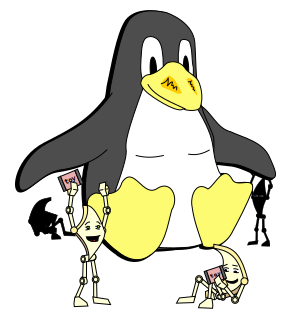
\includegraphics{cartoons/r-2014-Data-many-happy}}
\end{center}
\caption{Data Locking}
\ContributedBy{Figure}{fig:SMPdesign:Data Locking}{Melissa Broussard}
\end{figure}

% ./test_hash_spinlock.exe 1000 0/100 1 1024 1
% ./test_hash_spinlock.exe: nmilli: 1000 update/total: 0/100 nelements: 1 nbuckets: 1024 nthreads: 1
% ./test_hash_spinlock.exe: avg = 158.118  max = 162.404  min = 156.199  std = 2.19391
% ./test_hash_spinlock.exe: nmilli: 1000 update/total: 0/100 nelements: 1 nbuckets: 1024 nthreads: 1
% ./test_hash_spinlock.exe: avg = 157.717  max = 162.446  min = 156.415  std = 2.36662
% ./test_hash_spinlock.exe: nmilli: 1000 update/total: 0/100 nelements: 1 nbuckets: 1024 nthreads: 1
% ./test_hash_spinlock.exe: avg = 158.369  max = 164.75  min = 156.501  std = 3.19454

% ./test_hash_spinlock.exe 1000 0/100 1 1024 2
% ./test_hash_spinlock.exe: nmilli: 1000 update/total: 0/100 nelements: 1 nbuckets: 1024 nthreads: 2
% ./test_hash_spinlock.exe: avg = 223.426  max = 422.948  min = 167.858  std = 100.136
% ./test_hash_spinlock.exe: nmilli: 1000 update/total: 0/100 nelements: 1 nbuckets: 1024 nthreads: 2
% ./test_hash_spinlock.exe: avg = 235.462  max = 507.134  min = 167.466  std = 135.836
% ./test_hash_spinlock.exe: nmilli: 1000 update/total: 0/100 nelements: 1 nbuckets: 1024 nthreads: 2
% ./test_hash_spinlock.exe: avg = 305.807  max = 481.685  min = 167.939  std = 132.589

However, as those who have taken care of small children can again attest,
even providing enough to go around is no guarantee of tranquillity.
The analogous situation can arise in SMP programs.
For example, the Linux kernel maintains a cache of files and directories
(called ``dcache'').
Each entry in this cache has its own lock, but the entries corresponding
to the root directory and its direct descendants are much more likely to
be traversed than are more obscure entries.
This can result in many CPUs contending for the locks of these popular
entries, resulting in a situation not unlike that
shown in Figure~\ref{fig:SMPdesign:Data and Skew}.

\begin{figure}[htb]
\begin{center}
\resizebox{3in}{!}{
\includegraphics{cartoons/r-2014-Data-many-fighting}}
\end{center}
\caption{Data Locking and Skew}
\ContributedBy{Figure}{fig:SMPdesign:Data and Skew}{Melissa Broussard}
\end{figure}

In many cases, algorithms can be designed to reduce the instance of
data skew, and in some cases eliminate it entirely
(as appears to be possible with the Linux kernel's dcache~\cite{McKenney04a}).
Data locking is often used for partitionable data structures such as
hash tables, as well as in situations where multiple entities are each
represented by an instance of a given data structure.
The task list in version 2.6.17 of the Linux kernel is an example of the
latter, each task structure having its own \co{proc_lock}.

A key challenge with data locking on dynamically allocated structures
is ensuring that the structure remains in existence while the lock is
being acquired.
The code in
Figure~\ref{fig:SMPdesign:Data-Locking Hash Table Search}
finesses this challenge by placing the locks in the statically allocated
hash buckets, which are never freed.
However, this trick would not work if the hash table were resizeable,
so that the locks were now dynamically allocated.
In this case, there would need to be some means to prevent the hash
bucket from being freed during the time that its lock was being acquired.

\QuickQuiz{}
	What are some ways of preventing a structure from being freed while
	its lock is being acquired?
\QuickQuizAnswer{
	Here are a few possible solutions to this \emph{existence guarantee}
	problem:

	\begin{enumerate}
	\item	Provide a statically allocated lock that is held while
		the per-structure lock is being acquired, which is an
		example of hierarchical locking (see
		Section~\ref{sec:SMPdesign:Hierarchical Locking}).
		Of course, using a single global lock for this purpose
		can result in unacceptably high levels of lock contention,
		dramatically reducing performance and scalability.
	\item	Provide an array of statically allocated locks, hashing
		the structure's address to select the lock to be acquired,
		as described in Chapter~\ref{chp:Locking}.
		Given a hash function of sufficiently high quality, this
		avoids the scalability limitations of the single global
		lock, but in read-mostly situations, the lock-acquisition
		overhead can result in unacceptably degraded performance.
	\item	Use a garbage collector, in software environments providing
		them, so that a structure cannot be deallocated while being
		referenced.
		This works very well, removing the existence-guarantee
		burden (and much else besides) from the developer's
		shoulders, but imposes the overhead of garbage collection
		on the program.
		Although garbage-collection technology has advanced
		considerably in the past few decades, its overhead
		may be unacceptably high for some applications.
		In addition, some applications require that the developer
		exercise more control over the layout and placement of
		data structures than is permitted by most garbage collected
		environments.
	\item	As a special case of a garbage collector, use a global
		reference counter, or a global array of reference counters.
	\item	Use \emph{hazard pointers}~\cite{MagedMichael04a}, which
		can be thought of as an inside-out reference count.
		Hazard-pointer-based algorithms maintain a per-thread list of
		pointers, so that the appearance of a given pointer on
		any of these lists acts as a reference to the corresponding
		structure.
		Hazard pointers are an interesting research direction, but
		have not yet seen much use in production (written in 2008).
	\item	Use transactional memory
		(TM)~\cite{Herlihy93a,DBLomet1977SIGSOFT,Shavit95},
		so that each reference and
		modification to the data structure in question is
		performed atomically.
		Although TM has engendered much excitement in recent years,
		and seems likely to be of some use in production software,
		developers should exercise some
		caution~\cite{Blundell2005DebunkTM,Blundell2006TMdeadlock,McKenney2007PLOSTM},
		particularly in performance-critical code.
		In particular, existence guarantees require that the
		transaction cover the full path from a global reference
		to the data elements being updated.
	\item	Use RCU, which can be thought of as an extremely lightweight
		approximation to a garbage collector.
		Updaters are not permitted to free RCU-protected
		data structures that RCU readers might still be referencing.
		RCU is most heavily used for read-mostly data structures,
		and is discussed at length in
		Chapter~\ref{chp:Deferred Processing}.
	\end{enumerate}

	For more on providing existence guarantees, see
	Chapters~\ref{chp:Locking} and \ref{chp:Deferred Processing}.
} \QuickQuizEnd

\subsection{Data Ownership}
\label{sec:SMPdesign:Data Ownership}

Data ownership partitions a given data structure over the threads
or CPUs, so that each thread/CPU accesses its subset of the data
structure without any synchronization overhead whatsoever.
However, if one thread wishes to access some other thread's data,
the first thread is unable to do so directly.
Instead, the first thread must communicate with the second thread,
so that the second thread performs the operation on behalf of the
first, or, alternatively, migrates the data to the first thread.

Data ownership might seem arcane, but it is used very frequently:
\begin{enumerate}
\item	Any variables accessible by only one CPU or thread
	(such as {\tt auto} variables in C
	and C++) are owned by that CPU or process.
\item	An instance of a user interface owns the corresponding
	user's context.  It is very common for applications
	interacting with parallel database engines to be
	written as if they were entirely sequential programs.
	Such applications own the user interface and his current
	action.  Explicit parallelism is thus confined to the
	database engine itself.
\item	Parametric simulations are often trivially parallelized
	by granting each thread ownership of a particular region
	of the parameter space.
	There are also computing frameworks designed for this
	type of problem~\cite{BOINC2008}.
\end{enumerate}

If there is significant sharing, communication between the threads
or CPUs can result in significant complexity and overhead.
Furthermore, if the most-heavily used data happens to be that owned
by a single CPU, that CPU will be a ``hot spot'', sometimes with
results resembling that shown in Figure~\ref{fig:SMPdesign:Data and Skew}.
However, in situations where no sharing is required, data ownership
achieves ideal performance, and with code that can be as simple
as the sequential-program case shown in
Figure~\ref{fig:SMPdesign:Sequential-Program Hash Table Search}.
Such situations are often referred to as ``embarrassingly
parallel'', and, in the best case, resemble the situation
previously shown in Figure~\ref{fig:SMPdesign:Data Locking}.

% ./test_hash_null.exe 1000 0/100 1 1024 1
% ./test_hash_null.exe: nmilli: 1000 update/total: 0/100 nelements: 1 nbuckets: 1024 nthreads: 1
% ./test_hash_null.exe: avg = 96.2913  max = 98.2337  min = 90.4095  std = 2.95314
% ./test_hash_null.exe: nmilli: 1000 update/total: 0/100 nelements: 1 nbuckets: 1024 nthreads: 1
% ./test_hash_null.exe: avg = 91.5592  max = 97.3315  min = 89.9885  std = 2.88925
% ./test_hash_null.exe: nmilli: 1000 update/total: 0/100 nelements: 1 nbuckets: 1024 nthreads: 1
% ./test_hash_null.exe: avg = 93.3568  max = 106.162  min = 89.8828  std = 6.40418

% ./test_hash_null.exe 1000 0/100 1 1024 2
% ./test_hash_null.exe: nmilli: 1000 update/total: 0/100 nelements: 1 nbuckets: 1024 nthreads: 2
% ./test_hash_null.exe: avg = 45.4526  max = 46.4281  min = 45.1954  std = 0.487791
% ./test_hash_null.exe: nmilli: 1000 update/total: 0/100 nelements: 1 nbuckets: 1024 nthreads: 2
% ./test_hash_null.exe: avg = 46.0238  max = 49.2861  min = 45.1852  std = 1.63127
% ./test_hash_null.exe: nmilli: 1000 update/total: 0/100 nelements: 1 nbuckets: 1024 nthreads: 2
% ./test_hash_null.exe: avg = 46.6858  max = 52.6278  min = 45.1761  std = 2.97102

Another important instance of data ownership occurs when the data
is read-only, in which case,
all threads can ``own'' it via replication.

Data ownership will be presented in more detail in
Chapter~\ref{chp:Data Ownership}.

\subsection{Locking Granularity and Performance}
\label{sec:SMPdesign:Locking Granularity and Performance}

This section looks at locking granularity and performance from
a mathematical synchronization-efficiency viewpoint.
Readers who are uninspired by mathematics might choose to skip
this section.

The approach is to use a crude queueing model for the efficiency of
synchronization mechanism that operate on a single shared global
variable, based on an M/M/1 queue.
M/M/1 queuing models are based on an exponentially distributed
``inter-arrival rate'' $\lambda$ and an exponentially distributed
``service rate'' $\mu$.
The inter-arrival rate $\lambda$ can be thought of as the average
number of synchronization operations per second that the system
would process if the synchronization were free, in other words,
$\lambda$ is an inverse measure of the overhead of each non-synchronization
unit of work.
For example, if each unit of work was a transaction, and if each transaction
took one millisecond to process, excluding synchronization overhead,
then $\lambda$ would be 1,000 transactions per second.

The service rate $\mu$ is defined similarly, but for the average
number of synchronization operations per second that the system
would process if the overhead of each transaction was zero, and
ignoring the fact that CPUs must wait on each other to complete
their synchronization operations, in other words, $\mu$ can be roughly
thought of as the synchronization overhead in absence of contention.
For example, suppose that each synchronization operation involves an atomic
increment instruction, and that a computer system is able to do
an atomic increment every 25 nanoseconds on each CPU
to a private variable.\footnote{
	Of course, if there are 8 CPUs all incrementing the same
	shared variable, then each CPU must wait at least 175 nanoseconds
	for each of the other CPUs to do its increment before consuming
	an additional 25 nanoseconds doing its own increment.
	In actual fact, the wait will be longer due to the need
	to move the variable from one CPU to another.}
The value of $\mu$ is therefore about 40,000,000 atomic increments
per second.

Of course, the value of $\lambda$ increases with increasing numbers of
CPUs, as each CPU is capable of processing transactions independently
(again, ignoring synchronization):

\begin{equation}
	\lambda = n \lambda_0
\end{equation}

where $n$ is the number of CPUs and $\lambda_0$ is the transaction-processing
capability of a single CPU.
Note that the expected time for a single CPU to execute a single transaction
is $1 / \lambda_0$.

Because the CPUs have to ``wait in line'' behind each other to get their
chance to increment the single shared variable, we can use the M/M/1
queueing-model expression for the expected total waiting time:

\begin{equation}
	T = \frac{1}{\mu - \lambda}
\end{equation}

Substituting the above value of $\lambda$:

\begin{equation}
	T = \frac{1}{\mu - n \lambda_0}
\end{equation}

Now, the efficiency is just the ratio of the time required to process
a transaction in absence of synchronization ($1 / \lambda_0$)
to the time required including synchronization ($T + 1 / \lambda_0$):

\begin{equation}
	e = \frac{1 / \lambda_0}{T + 1 / \lambda_0}
\end{equation}

Substituting the above value for $T$ and simplifying:

\begin{equation}
	e = \frac{\frac{\mu}{\lambda_0} - n}{\frac{\mu}{\lambda_0} - (n - 1)}
\end{equation}

But the value of $\mu / \lambda_0$ is just the ratio of the time required
to process the transaction (absent synchronization overhead) to that of 
the synchronization overhead itself (absent contention).
If we call this ratio $f$, we have:

\begin{equation}
	e = \frac{f - n}{f - (n - 1)}
\end{equation}

\begin{figure}[tbp]
\begin{center}
\resizebox{3in}{!}{\includegraphics{SMPdesign/synceff}}
\end{center}
\caption{Synchronization Efficiency}
\label{fig:SMPdesign:Synchronization Efficiency}
\end{figure}

Figure~\ref{fig:SMPdesign:Synchronization Efficiency} plots the synchronization
efficiency $e$ as a function of the number of CPUs/threads $n$ for
a few values of the overhead ratio $f$.
For example, again using the 25-nanosecond atomic increment, the
$f=10$ line corresponds to each CPU attempting an atomic increment
every 250 nanoseconds, and the $f=100$ line corresponds to each
CPU attempting an atomic increment every 2.5 microseconds,
which in turn corresponds to several thousand instructions.
Given that each trace drops off sharply with increasing numbers of
CPUs or threads, we can conclude that
synchronization mechanisms based on
atomic manipulation of a single global shared variable will not
scale well if used heavily on current commodity hardware.
This is a mathematical depiction of the forces leading to the parallel
counting algorithms that were discussed in Chapter~\ref{chp:Counting}.

The concept of efficiency is useful even in cases having little or
no formal synchronization.
Consider for example a matrix multiply, in which the columns of one
matrix are multiplied (via ``dot product'') by the rows of another,
resulting in an entry in a third matrix.
Because none of these operations conflict, it is possible to partition
the columns of the first matrix among a group of threads, with each thread
computing the corresponding columns of the result matrix.
The threads can therefore operate entirely independently, with no
synchronization overhead whatsoever, as is done in
\texttt{matmul.c}.
One might therefore expect a parallel matrix multiply to have a
perfect efficiency of 1.0.

\begin{figure}[tbp]
\begin{center}
\resizebox{3in}{!}{\includegraphics{SMPdesign/matmuleff}}
\end{center}
\caption{Matrix Multiply Efficiency}
\label{fig:SMPdesign:Matrix Multiply Efficiency}
\end{figure}

However,
Figure~\ref{fig:SMPdesign:Matrix Multiply Efficiency}
tells a different story, especially for a 64-by-64 matrix multiply,
which never gets above an efficiency of about 0.7, even when running
single-threaded.
The 512-by-512 matrix multiply's efficiency is measurably less
than 1.0 on as few as 10 threads, and even the 1024-by-1024 matrix
multiply deviates noticeably from perfection at a few tens of threads.
Nevertheless, this figure clearly demonstrates the performance and
scalability benefits of batching: If you must incur synchronization
overhead, you may as well get your money's worth.

\QuickQuiz{}
	How can a single-threaded 64-by-64 matrix multiple possibly
	have an efficiency of less than 1.0?
	Shouldn't all of the traces in
	Figure~\ref{fig:SMPdesign:Matrix Multiply Efficiency}
	have efficiency of exactly 1.0 when running on only one thread?
\QuickQuizAnswer{
	The \texttt{matmul.c} program creates the specified number of
	worker threads, so even the single-worker-thread case incurs
	thread-creation overhead.
	Making the changes required to optimize away thread-creation
	overhead in the single-worker-thread case is left as an
	exercise to the reader.
} \QuickQuizEnd

Given these inefficiencies,
it is worthwhile to look into more-scalable approaches
such as the data locking described in
Section~\ref{sec:SMPdesign:Data Locking}
or the parallel-fastpath approach discussed in the next section.

\QuickQuiz{}
	How are data-parallel techniques going to help with matrix
	multiply?
	It is \emph{already} data parallel!!!
\QuickQuizAnswer{
	I am glad that you are paying attention!
	This example serves to show that although data parallelism can
	be a very good thing, it is not some magic wand that automatically
	wards off any and all sources of inefficiency.
	Linear scaling at full performance, even to ``only'' 64 threads,
	requires care at all phases of design and implementation.

	In particular, you need to pay careful attention to the
	size of the partitions.
	For example, if you split a 64-by-64 matrix multiply across
	64 threads, each thread gets only 64 floating-point multiplies.
	The cost of a floating-point multiply is miniscule compared to
	the overhead of thread creation.

	Moral: If you have a parallel program with variable input,
	always include a check for the input size being too small to
	be worth parallelizing.
	And when it is not helpful to parallelize, it is not helpful
	to incur the overhead required to spawn a thread, now is it?
} \QuickQuizEnd

\section{Parallel Fastpath}
\label{sec:SMPdesign:Parallel Fastpath}

Fine-grained (and therefore \emph{usually} higher-performance)
designs are typically more complex than are coarser-grained designs.
In many cases, most of the overhead is incurred by a small fraction
of the code~\cite{Knuth73}.
So why not focus effort on that small fraction?

This is the idea behind the parallel-fastpath design pattern, to aggressively
parallelize the common-case code path without incurring the complexity
that would be required to aggressively parallelize the entire algorithm.
You must understand not only the specific algorithm you wish
to parallelize, but also the workload that the algorithm will
be subjected to.  Great creativity and design
effort is often required to construct a parallel fastpath.

Parallel fastpath combines different patterns (one for the
fastpath, one elsewhere) and is therefore a template pattern.
The following instances of parallel
fastpath occur often enough to warrant their own patterns,
as depicted in Figure~\ref{fig:SMPdesign:Parallel-Fastpath Design Patterns}:

\begin{figure}[htb]
\begin{center}
% \resizebox{3in}{!}{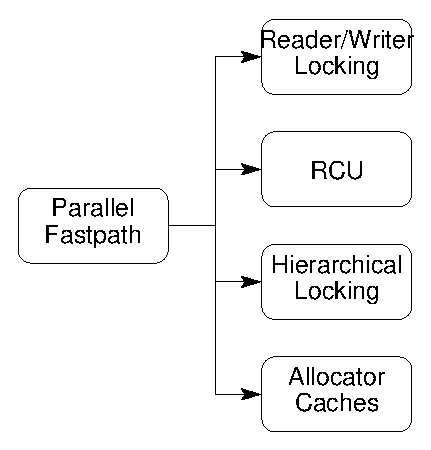
\includegraphics{SMPdesign/ParallelFastpath}}
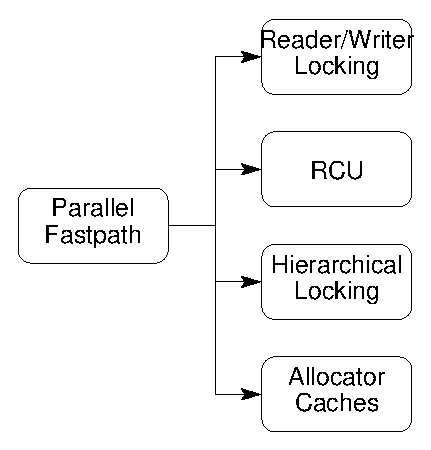
\includegraphics{SMPdesign/ParallelFastpath}
\end{center}
\caption{Parallel-Fastpath Design Patterns}
\label{fig:SMPdesign:Parallel-Fastpath Design Patterns}
\end{figure}

\begin{enumerate}
\item	Reader/Writer Locking
	(described below in Section~\ref{sec:SMPdesign:Reader/Writer Locking}).
\item	Read-copy update (RCU), which may be used as a high-performance
	replacement for reader/writer locking, is introduced in
	Section~\ref{sec:defer:Read-Copy Update (RCU)}, and will not
	be discussed further in this chapter.
\item   Hierarchical Locking~(\cite{McKenney95b}), which is touched upon
	in Section~\ref{sec:SMPdesign:Hierarchical Locking}.
\item	Resource Allocator Caches~(\cite{McKenney95b,McKenney93}).
	See Section~\ref{sec:SMPdesign:Resource Allocator Caches}
	for more detail.
\end{enumerate}

\subsection{Reader/Writer Locking}
\label{sec:SMPdesign:Reader/Writer Locking}

If synchronization overhead is negligible (for example, if the program
uses coarse-grained parallelism with large critical sections), and if
only a small fraction of the critical sections modify data, then allowing
multiple readers to proceed in parallel can greatly increase scalability.
Writers exclude both readers and each other.
There are many implementations of reader-writer locking, including
the POSIX implementation described in
Section~\ref{sec:toolsoftrade:POSIX Reader-Writer Locking}.
Figure~\ref{fig:SMPdesign:Reader-Writer-Locking Hash Table Search}
shows how the hash search might be implemented using reader-writer locking.

\begin{figure}[htbp]
{ \scriptsize
\begin{verbatim}
  1 rwlock_t hash_lock;
  2
  3 struct hash_table
  4 {
  5   long nbuckets;
  6   struct node **buckets;
  7 };
  8
  9 typedef struct node {
 10   unsigned long key;
 11   struct node *next;
 12 } node_t;
 13
 14 int hash_search(struct hash_table *h, long key)
 15 {
 16   struct node *cur;
 17   int retval;
 18
 19   read_lock(&hash_lock);
 20   cur = h->buckets[key % h->nbuckets];
 21   while (cur != NULL) {
 22     if (cur->key >= key) {
 23       retval = (cur->key == key);
 24       read_unlock(&hash_lock);
 25       return retval;
 26     }
 27     cur = cur->next;
 28   }
 29   read_unlock(&hash_lock);
 30   return 0;
 31 }
\end{verbatim}
}
\caption{Reader-Writer-Locking Hash Table Search}
\label{fig:SMPdesign:Reader-Writer-Locking Hash Table Search}
\end{figure}

Reader/writer locking is a simple instance of asymmetric locking.
Snaman~\cite{Snaman87} describes a more ornate six-mode
asymmetric locking design used in several clustered systems.
Locking in general and reader-writer locking in particular is described
extensively in
Chapter~\ref{chp:Locking}.

\subsection{Hierarchical Locking}
\label{sec:SMPdesign:Hierarchical Locking}

The idea behind hierarchical locking is to have a coarse-grained lock
that is held only long enough to work out which fine-grained lock
to acquire.
Figure~\ref{fig:SMPdesign:Hierarchical-Locking Hash Table Search}
shows how our hash-table search might be adapted to do hierarchical
locking, but also shows the great weakness of this approach:
we have paid the overhead of acquiring a second lock, but we only
hold it for a short time.
In this case, the simpler data-locking approach would be simpler
and likely perform better.

\begin{figure}[htbp]
{ \scriptsize
\begin{verbatim}
  1 struct hash_table
  2 {
  3   long nbuckets;
  4   struct bucket **buckets;
  5 };
  6
  7 struct bucket {
  8   spinlock_t bucket_lock;
  9   node_t *list_head;
 10 };
 11
 12 typedef struct node {
 13   spinlock_t node_lock;
 14   unsigned long key;
 15   struct node *next;
 16 } node_t;
 17
 18 int hash_search(struct hash_table *h, long key)
 19 {
 20   struct bucket *bp;
 21   struct node *cur;
 22   int retval;
 23
 24   bp = h->buckets[key % h->nbuckets];
 25   spin_lock(&bp->bucket_lock);
 26   cur = bp->list_head;
 27   while (cur != NULL) {
 28     if (cur->key >= key) {
 29       spin_lock(&cur->node_lock);
 30       spin_unlock(&bp->bucket_lock);
 31       retval = (cur->key == key);
 32       spin_unlock(&cur->node_lock);
 33       return retval;
 34     }
 35     cur = cur->next;
 36   }
 37   spin_unlock(&bp->bucket_lock);
 38   return 0;
 39 }
\end{verbatim}
}
\caption{Hierarchical-Locking Hash Table Search}
\label{fig:SMPdesign:Hierarchical-Locking Hash Table Search}
\end{figure}

\QuickQuiz{}
	In what situation would hierarchical locking work well?
\QuickQuizAnswer{
	If the comparison on line~31 of
	Figure~\ref{fig:SMPdesign:Hierarchical-Locking Hash Table Search}
	were replaced by a much heavier-weight operation,
	then releasing {\tt bp->bucket\_lock} \emph{might} reduce lock
	contention enough to outweigh the overhead of the extra
	acquisition and release of {\tt cur->node\_lock}.
} \QuickQuizEnd

\subsection{Resource Allocator Caches}
\label{sec:SMPdesign:Resource Allocator Caches}

This section presents a simplified schematic of a parallel fixed-block-size
memory allocator.
More detailed descriptions may be found in the
literature~\cite{McKenney92a,McKenney93,Bonwick01slab,McKenney01e}
or in the Linux kernel~\cite{Torvalds2.6kernel}.

\subsubsection{Parallel Resource Allocation Problem}

The basic problem facing a parallel memory allocator is the tension
between the need to provide extremely fast memory allocation and
freeing in the common case and the need to efficiently distribute
memory in face of unfavorable allocation and freeing patterns.

To see this tension, consider a straightforward application of
data ownership to this problem --- simply carve up memory so that
each CPU owns its share.
For example, suppose that a system with two CPUs has two gigabytes
of memory (such as the one that I am typing on right now).
We could simply assign each CPU one gigabyte of memory, and allow
each CPU to access its own private chunk of memory, without the
need for locking and its complexities and overheads.
Unfortunately, this simple scheme breaks down if an algorithm happens
to have CPU 0 allocate all of the memory and CPU 1 the free it, as
would happen in a simple producer-consumer workload.

The other extreme, code locking, suffers from excessive lock contention
and overhead~\cite{McKenney93}.

\subsubsection{Parallel Fastpath for Resource Allocation}

The commonly used solution uses parallel fastpath with each CPU
owning a modest cache of blocks, and with a large code-locked
shared pool for additional blocks.
To prevent any given CPU from monopolizing the memory blocks,
we place a limit on the number of blocks that can be in each CPU's
cache.
In a two-CPU system, the flow of memory blocks will be as shown
in Figure~\ref{fig:SMPdesign:Allocator Cache Schematic}:
when a given CPU is trying to free a block when its pool is full,
it sends blocks to the global pool, and, similarly, when that CPU
is trying to allocate a block when its pool is empty, it retrieves
blocks from the global pool.

\begin{figure}[htb]
\begin{center}
\resizebox{3in}{!}{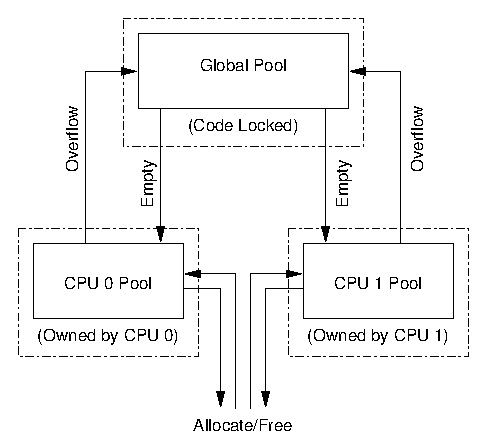
\includegraphics{SMPdesign/allocatorcache}}
\end{center}
\caption{Allocator Cache Schematic}
\label{fig:SMPdesign:Allocator Cache Schematic}
\end{figure}

\subsubsection{Data Structures}

The actual data structures for a ``toy'' implementation of allocator
caches are shown in
Figure~\ref{fig:SMPdesign:Allocator-Cache Data Structures}.
The ``Global Pool'' of Figure~\ref{fig:SMPdesign:Allocator Cache Schematic}
is implemented by \co{globalmem} of type \co{struct globalmempool},
and the two CPU pools by the per-CPU variable \co{percpumem} of
type \co{percpumempool}.
Both of these data structures have arrays of pointers to blocks
in their \co{pool} fields, which are filled from index zero upwards.
Thus, if \co{globalmem.pool[3]} is \co{NULL}, then the remainder of
the array from index 4 up must also be NULL.
The \co{cur} fields contain the index of the highest-numbered full
element of the \co{pool} array, or -1 if all elements are empty.
All elements from \co{globalmem.pool[0]} through
\co{globalmem.pool[globalmem.cur]} must be full, and all the rest
must be empty.\footnote{
	Both pool sizes (\co{TARGET_POOL_SIZE} and
	\co{GLOBAL_POOL_SIZE}) are unrealistically small, but this small
	size makes it easier to single-step the program in order to get
	a feel for its operation.}

\begin{figure}[htbp]
{ \scriptsize
\begin{verbatim}
  1 #define TARGET_POOL_SIZE 3
  2 #define GLOBAL_POOL_SIZE 40
  3
  4 struct globalmempool {
  5   spinlock_t mutex;
  6   int cur;
  7   struct memblock *pool[GLOBAL_POOL_SIZE];
  8 } globalmem;
  9
 10 struct percpumempool {
 11   int cur;
 12   struct memblock *pool[2 * TARGET_POOL_SIZE];
 13 };
 14
 15 DEFINE_PER_THREAD(struct percpumempool, percpumem);
\end{verbatim}
}
\caption{Allocator-Cache Data Structures}
\label{fig:SMPdesign:Allocator-Cache Data Structures}
\end{figure}

The operation of the pool data structures is illustrated by
Figure~\ref{fig:SMPdesign:Allocator Pool Schematic},
with the six boxes representing the array of pointers making up
the \co{pool} field, and the number preceding them representing
the \co{cur} field.
The shaded boxes represent non-\co{NULL} pointers, while the empty
boxes represent \co{NULL} pointers.
An important, though potentially confusing, invariant of this
data structure is that the \co{cur} field is always one
smaller than the number of non-\co{NULL} pointers.

\begin{figure}[htb]
\begin{center}
\resizebox{3in}{!}{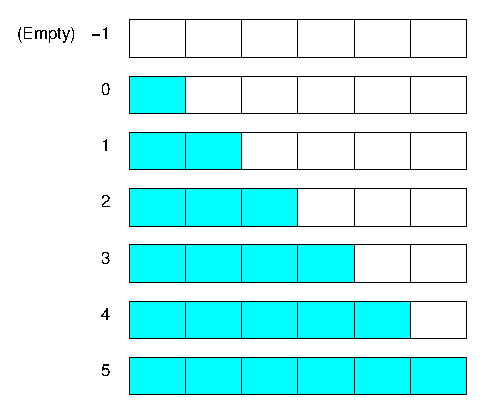
\includegraphics{SMPdesign/AllocatorPool}}
\end{center}
\caption{Allocator Pool Schematic}
\label{fig:SMPdesign:Allocator Pool Schematic}
\end{figure}

\subsubsection{Allocation Function}

The allocation function \co{memblock_alloc()} may be seen in
Figure~\ref{fig:SMPdesign:Allocator-Cache Allocator Function}.
Line~7 picks up the current thread's per-thread pool,
and line~8 check to see if it is empty.

If so, lines~9-16 attempt to refill it from the global pool
under the spinlock acquired on line~9 and released on line~16.
Lines~10-14 move blocks from the global to the per-thread pool until
either the local pool reaches its target size (half full) or
the global pool is exhausted, and line~15 sets the per-thread pool's
count to the proper value.

In either case, line~18 checks for the per-thread pool still being
empty, and if not, lines~19-21 remove a block and return it.
Otherwise, line~23 tells the sad tale of memory exhaustion.

\begin{figure}[htbp]
{ \scriptsize
\begin{verbatim}
  1 struct memblock *memblock_alloc(void)
  2 {
  3   int i;
  4   struct memblock *p;
  5   struct percpumempool *pcpp;
  6
  7   pcpp = &__get_thread_var(percpumem);
  8   if (pcpp->cur < 0) {
  9     spin_lock(&globalmem.mutex);
 10     for (i = 0; i < TARGET_POOL_SIZE &&
 11                 globalmem.cur >= 0; i++) {
 12       pcpp->pool[i] = globalmem.pool[globalmem.cur];
 13       globalmem.pool[globalmem.cur--] = NULL;
 14     }
 15     pcpp->cur = i - 1;
 16     spin_unlock(&globalmem.mutex);
 17   }
 18   if (pcpp->cur >= 0) {
 19     p = pcpp->pool[pcpp->cur];
 20     pcpp->pool[pcpp->cur--] = NULL;
 21     return p;
 22   }
 23   return NULL;
 24 }
\end{verbatim}
}
\caption{Allocator-Cache Allocator Function}
\label{fig:SMPdesign:Allocator-Cache Allocator Function}
\end{figure}

\subsubsection{Free Function}

Figure~\ref{fig:SMPdesign:Allocator-Cache Free Function} shows
the memory-block free function.
Line~6 gets a pointer to this thread's pool, and
line~7 checks to see if this per-thread pool is full.

If so, lines~8-15 empty half of the per-thread pool into the global pool,
with lines~8 and 14 acquiring and releasing the spinlock.
Lines~9-12 implement the loop moving blocks from the local to the
global pool, and line~13 sets the per-thread pool's count to the proper
value.

In either case, line~16 then places the newly freed block into the
per-thread pool.

\begin{figure}[htbp]
{ \scriptsize
\begin{verbatim}
  1 void memblock_free(struct memblock *p)
  2 {
  3   int i;
  4   struct percpumempool *pcpp;
  5
  6   pcpp = &__get_thread_var(percpumem);
  7   if (pcpp->cur >= 2 * TARGET_POOL_SIZE - 1) {
  8     spin_lock(&globalmem.mutex);
  9     for (i = pcpp->cur; i >= TARGET_POOL_SIZE; i--) {
 10       globalmem.pool[++globalmem.cur] = pcpp->pool[i];
 11       pcpp->pool[i] = NULL;
 12     }
 13     pcpp->cur = i;
 14     spin_unlock(&globalmem.mutex);
 15   }
 16   pcpp->pool[++pcpp->cur] = p;
 17 }
\end{verbatim}
}
\caption{Allocator-Cache Free Function}
\label{fig:SMPdesign:Allocator-Cache Free Function}
\end{figure}

\subsubsection{Performance}

Rough performance results\footnote{
	This data was not collected in a statistically meaningful way,
	and therefore should be viewed with great skepticism and suspicion.
	Good data-collection and -reduction practice is discussed
	in Chapter~\ref{chp:Validation}.
	That said, repeated runs gave similar results, and these results
	match more careful evaluations of similar algorithms.}
are shown in
Figure~\ref{fig:SMPdesign:Allocator Cache Performance},
running on a dual-core Intel x86 running at 1GHz (4300 bogomips per CPU)
with at most six blocks allowed in each CPU's cache.
In this micro-benchmark,
each thread repeatedly allocates a group of blocks and then frees all
the blocks in that group, with
the number of blocks in the group being the ``allocation run length''
displayed on the x-axis.
The y-axis shows the number of successful allocation/free pairs per
microsecond --- failed allocations are not counted.
The ``X''s are from a two-thread run, while the ``+''s are from a
single-threaded run.

\begin{figure}[htb]
\begin{center}
\resizebox{3in}{!}{\includegraphics{SMPdesign/smpalloc}}
\end{center}
\caption{Allocator Cache Performance}
\label{fig:SMPdesign:Allocator Cache Performance}
\end{figure}

Note that run lengths up to six scale linearly and give excellent performance,
while run lengths greater than six show poor performance and almost always
also show \emph{negative} scaling.
It is therefore quite important to size \co{TARGET_POOL_SIZE}
sufficiently large,
which fortunately is usually quite easy to do in actual
practice~\cite{McKenney01e}, especially given today's large memories.
For example, in most systems, it is quite reasonable to set
\co{TARGET_POOL_SIZE} to 100, in which case allocations and frees
are guaranteed to be confined to per-thread pools at least 99\% of
the time.

As can be seen from the figure, the situations where the common-case
data-ownership applies (run lengths up to six) provide greatly improved
performance compared to the cases where locks must be acquired.
Avoiding synchronization in the common case will be a recurring theme through
this book.

\QuickQuiz{}
	In Figure~\ref{fig:SMPdesign:Allocator Cache Performance},
	there is a pattern of performance rising with increasing run
	length in groups of three samples, for example, for run lengths
	10, 11, and 12.
	Why?
\QuickQuizAnswer{
	This is due to the per-CPU target value being three.
	A run length of 12 must acquire the global-pool lock twice,
	while a run length of 13 must acquire the global-pool lock
	three times.
} \QuickQuizEnd

\QuickQuiz{}
	Allocation failures were observed in the two-thread
	tests at run lengths of 19 and greater.
	Given the global-pool size of 40 and the per-thread target
	pool size $s$ of three, number of threads $n$ equal to two,
	and assuming that the per-thread pools are initially
	empty with none of the memory in use, what is the smallest allocation
	run length $m$ at which failures can occur?
	(Recall that each thread repeatedly allocates $m$ block of memory,
	and then frees the $m$ blocks of memory.)
	Alternatively, given $n$ threads each with pool size $s$, and
	where each thread repeatedly first allocates $m$ blocks of memory
	and then frees those $m$ blocks, how large must the global pool
	size be?
	\emph{Note:} Obtaining the correct answer will require you to
	examine the \co{smpalloc.c} source code, and very likely
	single-step it as well.
	You have been warned!
\QuickQuizAnswer{
	This solution is adapted from one put forward by Alexey Roytman.
	It is based on the following definitions:

	\begin{description}
	\item[$g$]	Number of blocks globally available.
	\item[$i$]	Number of blocks left in the initializing thread's
			per-thread pool.  (This is one reason you needed
			to look at the code!)
	\item[$m$]	Allocation/free run length.
	\item[$n$]	Number of threads, excluding the initialization thread.
	\item[$p$]	Per-thread maximum block consumption, including
			both the blocks actually allocated and the blocks
			remaining in the per-thread pool.
	\end{description}

	The values $g$, $m$, and $n$ are given.  The value for $p$ is
	$m$ rounded up to the next multiple of $s$, as follows:

	\begin{equation}
		p = s \left \lfloor \frac{m + s - 1}{s} \right \rfloor
	\label{sec:SMPdesign:p}
	\end{equation}

	The value for $i$ is as follows:

	\begin{equation}
		i = \left \{
			\begin{array}{l}
				g \pmod{2 s} = 0: 2 s \\
				g \pmod{2 s} \ne 0: g \pmod{2 s}
			\end{array}
		    \right .
	\label{sec:SMPdesign:i}
	\end{equation}

	\begin{figure}[tb]
	\begin{center}
	\resizebox{3in}{!}{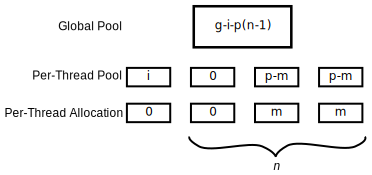
\includegraphics{SMPdesign/smpalloclim}}
	\end{center}
	\caption{Allocator Cache Run-Length Analysis}
	\label{fig:SMPdesign:Allocator Cache Run-Length Analysis}
	\end{figure}

	The relationships between these quantities is shown in
	Figure~\ref{fig:SMPdesign:Allocator Cache Run-Length Analysis}.
	The global pool is shown on the top of this figure, and
	the ``extra'' initializer thread's per-thread pool and
	per-thread allocations are the left-most pair of boxes.
	The initializer thread has no blocks allocated, but has
	$i$ blocks stranded in its per-thread pool.
	The rightmost two pairs of boxes are the per-thread pools and
	per-thread allocations of threads holding the maximum possible
	number of blocks, while the second-from-left pair of boxes
	represents the thread currently trying to allocate.

	The total number of blocks is $g$, and adding up the per-thread
	allocations and per-thread pools, we see that the global pool
	contains $g-i-p(n-1)$ blocks.
	If the allocating thread is to be successful, it needs at least
	$m$ blocks in the global pool, in other words:

	\begin{equation}
		g - i - p(n - 1) \ge m
	\label{sec:SMPdesign:g-vs-m}
	\end{equation}

	The question has $g=40$, $s=3$, and $n=2$.
	Equation~\ref{sec:SMPdesign:i} gives $i=4$, and
	Equation~\ref{sec:SMPdesign:p} gives $p=18$ for $m=18$
	and $p=21$ for $m=19$.
	Plugging these into Equation~\ref{sec:SMPdesign:g-vs-m}
	shows that $m=18$ will not overflow, but that $m=19$ might
	well do so.

	The presence of $i$ could be considered to be a bug.
	After all, why allocate memory only to have it stranded in
	the initialization thread's cache?
	One way of fixing this would be to provide a \co{memblock_flush()}
	function that flushed the current thread's pool into the
	global pool.
	The initialization thread could then invoke this function
	after freeing all of the blocks.
} \QuickQuizEnd

\subsubsection{Real-World Design}

The toy parallel resource allocator was quite simple, but real-world
designs expand on this approach in a number of ways.

First, real-world allocators are required to handle a wide range
of allocation sizes, as opposed to the single size shown in this
toy example.
One popular way to do this is to offer a fixed set of sizes, spaced
so as to balance external and internal fragmentation, such as in
the late-1980s BSD memory allocator~\cite{McKusick88}.
Doing this would mean that the ``globalmem'' variable would need
to be replicated on a per-size basis, and that the associated
lock would similarly be replicated, resulting in data locking
rather than the toy program's code locking.

Second, production-quality systems must be able to repurpose memory,
meaning that they must be able to coalesce blocks into larger structures,
such as pages~\cite{McKenney93}.
This coalescing will also need to be protected by a lock, which again
could be replicated on a per-size basis.

Third, coalesced memory must be returned to the underlying memory
system, and pages of memory must also be allocated from the underlying
memory system.
The locking required at this level will depend on that of the underlying
memory system, but could well be code locking.
Code locking can often be tolerated at this level, because this
level is so infrequently reached in well-designed systems~\cite{McKenney01e}.

Despite this real-world design's greater complexity, the underlying
idea is the same --- repeated application of parallel fastpath,
as shown in
Table~\ref{fig:app:questions:Schematic of Real-World Parallel Allocator}.

\begin{table}[htbp]
{ \scriptsize
\begin{tabular}{l|l|p{1in}}
Level	& Locking & Purpose \\
\hline
Per-thread pool	  & Data ownership & High-speed allocation \\
Global block pool & Data locking   & Distributing blocks among threads \\
Coalescing	  & Data locking   & Combining blocks into pages \\
System memory	  & Code locking   & Memory from/to system \\
\end{tabular}
}
\caption{Schematic of Real-World Parallel Allocator}
\label{fig:app:questions:Schematic of Real-World Parallel Allocator}
\end{table}

% SMPdesign/beyond.tex
% mainfile: ../perfbook.tex
% SPDX-License-Identifier: CC-BY-SA-3.0

\section{Beyond Partitioning}
\label{sec:SMPdesign:Beyond Partitioning}
\OriginallyPublished{Section}{sec:SMPdesign:Beyond Partitioning}{Retrofitted Parallelism Considered Grossly Sub-Optimal}{4\textsuperscript{th} USENIX Workshop on Hot Topics on Parallelism}{PaulEMcKenney2012HOTPARsuboptimal}
%
\epigraph{It is all right to aim high if you have plenty of ammunition.}
	 {\emph{Hawley R. Everhart}}

This chapter has discussed how data partitioning can be used to design
simple linearly scalable parallel programs.
Section~\ref{sec:SMPdesign:Data Ownership} hinted at the possibilities
of data replication, which will be used to great effect in
Section~\ref{sec:defer:Read-Copy Update (RCU)}.

The main goal of applying partitioning and replication is to achieve
linear speedups, in other words, to ensure that the total amount of
work required does not increase significantly as the number of CPUs
or threads increases.
A problem that can be solved via partitioning and/or replication,
resulting in linear speedups, is \emph{embarrassingly parallel}.
But can we do better?

To answer this question, let us examine the solution of
labyrinths and mazes.
Of course, labyrinths and mazes have been objects of fascination for
millennia~\cite{WikipediaLabyrinth},
so it should come as no surprise that they are generated and solved
using computers, including biological
computers~\cite{AndrewAdamatzky2011SlimeMold},
GPGPUs~\cite{ChristerEricson2008GPUMaze}, and even
discrete hardware~\cite{MIT:TRMag:MemristorMazes}.
Parallel solution of mazes is sometimes used as a class project in
universities~\cite{ETHZurich:FS2011maze,UMD:CMSC433maze} and
as a vehicle to demonstrate the benefits of parallel-programming
frameworks~\cite{RonFosner2010maze}.

Common advice is to use a parallel work-queue algorithm
(PWQ)~\cite{ETHZurich:FS2011maze,RonFosner2010maze}.
This section evaluates this advice by comparing PWQ
against a sequential algorithm (SEQ) and also against
an alternative parallel algorithm, in all cases solving randomly generated
square mazes.
Section~\ref{sec:SMPdesign:Work-Queue Parallel Maze Solver} discusses PWQ,
Section~\ref{sec:SMPdesign:Alternative Parallel Maze Solver} discusses an alternative
parallel algorithm,
Section~\ref{sec:SMPdesign:Performance Comparison I} analyzes its anomalous performance,
Section~\ref{sec:SMPdesign:Alternative Sequential Maze Solver} derives an improved
sequential algorithm from the alternative parallel algorithm,
Section~\ref{sec:SMPdesign:Performance Comparison II} makes further performance
comparisons,
and finally
Section~\ref{sec:SMPdesign:Future Directions and Conclusions}
presents future directions and concluding remarks.

\subsection{Work-Queue Parallel Maze Solver}
\label{sec:SMPdesign:Work-Queue Parallel Maze Solver}

PWQ is based on SEQ, which is shown in
Listing~\ref{lst:SMPdesign:SEQ Pseudocode}
(pseudocode for \path{maze_seq.c}).
The maze is represented by a 2D array of cells and
a linear-array-based work queue named \co{->visited}.

\begin{listing}[tbp]
\begin{fcvlabel}[ln:SMPdesign:SEQ Pseudocode]
\begin{VerbatimL}[commandchars=\\\@\$]
int maze_solve(maze *mp, cell sc, cell ec)
{
	cell c = sc;
	cell n;
	int vi = 0;

	maze_try_visit_cell(mp, c, c, &n, 1);		\lnlbl@initcell$
	for (;;) {					\lnlbl@loop:b$
		while (!maze_find_any_next_cell(mp, c, &n)) {\lnlbl@loop2:b$
			if (++vi >= mp->vi)		\lnlbl@ifge$
				return 0;
			c = mp->visited[vi].c;
		}					\lnlbl@loop2:e$
		do {					\lnlbl@loop3:b$
			if (n == ec) {
				return 1;
			}
			c = n;
		} while (maze_find_any_next_cell(mp, c, &n));\lnlbl@loop3:e$
		c = mp->visited[vi].c;			\lnlbl@finalize$
	}						\lnlbl@loop:e$
}
\end{VerbatimL}
\end{fcvlabel}
\caption{SEQ Pseudocode}
\label{lst:SMPdesign:SEQ Pseudocode}
\end{listing}

\begin{fcvref}[ln:SMPdesign:SEQ Pseudocode]
Line~\lnref{initcell} visits the initial cell, and each iteration of the loop spanning
\clnrefrange{loop:b}{loop:e} traverses passages headed by one cell.
The loop spanning
\clnrefrange{loop2:b}{loop2:e} scans the \co{->visited[]} array for a
visited cell with an unvisited neighbor, and the loop spanning
\clnrefrange{loop3:b}{loop3:e} traverses one fork of the submaze
headed by that neighbor.
Line~\lnref{finalize} initializes for the next pass through the outer loop.
\end{fcvref}

\begin{listing}[tbp]
\begin{fcvlabel}[ln:SMPdesign:SEQ Helper Pseudocode]
\begin{VerbatimL}[commandchars=\\\@\$]
int maze_try_visit_cell(struct maze *mp, cell c, cell t, \lnlbl@try:b$
                        cell *n, int d)
{
	if (!maze_cells_connected(mp, c, t) ||	\lnlbl@try:chk:adj$
	    (*celladdr(mp, t) & VISITED))	\lnlbl@try:chk:not:visited$
		return 0;			\lnlbl@try:ret:failure$
	*n = t;					\lnlbl@try:nextcell$
	mp->visited[mp->vi] = t;		\lnlbl@try:recordnext$
	mp->vi++;				\lnlbl@try:next:visited$
	*celladdr(mp, t) |= VISITED | d;	\lnlbl@try:mark:visited$
	return 1;				\lnlbl@try:ret:success$
}						\lnlbl@try:e$

int maze_find_any_next_cell(struct maze *mp, cell c, \lnlbl@find:b$
                            cell *n)
{
	int d = (*celladdr(mp, c) & DISTANCE) + 1;	\lnlbl@find:curplus1$

	if (maze_try_visit_cell(mp, c, prevcol(c), n, d))\lnlbl@find:chk:prevcol$
		return 1;				\lnlbl@find:ret:prevcol$
	if (maze_try_visit_cell(mp, c, nextcol(c), n, d))\lnlbl@find:chk:nextcol$
		return 1;				\lnlbl@find:ret:nextcol$
	if (maze_try_visit_cell(mp, c, prevrow(c), n, d))\lnlbl@find:chk:prevrow$
		return 1;				\lnlbl@find:ret:prevrow$
	if (maze_try_visit_cell(mp, c, nextrow(c), n, d))\lnlbl@find:chk:nextrow$
		return 1;				\lnlbl@find:ret:nextrow$
	return 0;					\lnlbl@find:ret:false$
}							\lnlbl@find:e$
\end{VerbatimL}
\end{fcvlabel}
\caption{SEQ Helper Pseudocode}
\label{lst:SMPdesign:SEQ Helper Pseudocode}
\end{listing}

\begin{fcvref}[ln:SMPdesign:SEQ Helper Pseudocode:try]
The pseudocode for \co{maze_try_visit_cell()} is shown on
\clnrefrange{b}{e}
of Listing~\ref{lst:SMPdesign:SEQ Helper Pseudocode}
(\path{maze.c}).
Line~\lnref{chk:adj} checks to see if cells \co{c} and \co{t} are
adjacent and connected,
while line~\lnref{chk:not:visited} checks to see if cell \co{t} has
not yet been visited.
The \co{celladdr()} function returns the address of the specified cell.
If either check fails, line~\lnref{ret:failure} returns failure.
Line~\lnref{nextcell} indicates the next cell,
line~\lnref{recordnext} records this cell in the next
slot of the \co{->visited[]} array,
line~\lnref{next:visited} indicates that this slot
is now full, and line~\lnref{mark:visited} marks this cell as visited and also records
the distance from the maze start.  Line~\lnref{ret:success} then returns success.
\end{fcvref}

\begin{fcvref}[ln:SMPdesign:SEQ Helper Pseudocode:find]
The pseudocode for \co{maze_find_any_next_cell()} is shown on
\clnrefrange{b}{e}
of Listing~\ref{lst:SMPdesign:SEQ Helper Pseudocode}
(\path{maze.c}).
Line~\lnref{curplus1} picks up the current cell's distance plus 1,
while lines~\lnref{chk:prevcol}, \lnref{chk:nextcol}, \lnref{chk:prevrow},
and~\lnref{chk:nextrow}
check the cell in each direction, and
lines~\lnref{ret:prevcol}, \lnref{ret:nextcol}, \lnref{ret:prevrow},
and~\lnref{ret:nextrow}
return true if the corresponding cell is a candidate next cell.
The \co{prevcol()}, \co{nextcol()}, \co{prevrow()}, and \co{nextrow()}
each do the specified array-index-conversion operation.
If none of the cells is a candidate, line~\lnref{ret:false} returns false.
\end{fcvref}

\begin{figure}[tb]
\centering
\resizebox{1.2in}{!}{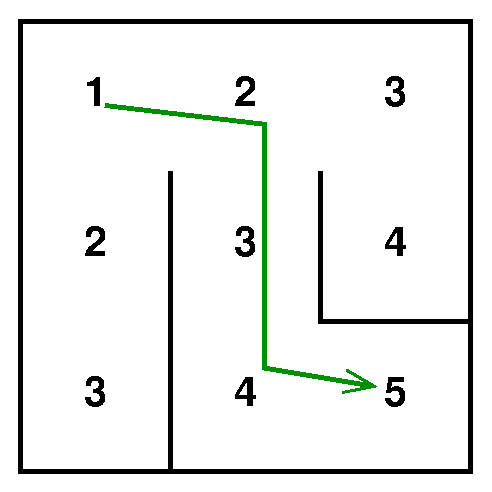
\includegraphics{SMPdesign/MazeNumberPath}}
\caption{Cell-Number Solution Tracking}
\label{fig:SMPdesign:Cell-Number Solution Tracking}
\end{figure}

The path is recorded in the maze by counting the number of cells from
the starting point, as shown in
Figure~\ref{fig:SMPdesign:Cell-Number Solution Tracking},
where the starting cell is in the upper left and the ending cell is
in the lower right.
Starting at the ending cell and following
consecutively decreasing cell numbers traverses the solution.

\begin{figure}[tb]
\centering
\resizebox{2.2in}{!}{\includegraphics{SMPdesign/500-ms_seq_fg-cdf}}
\caption{CDF of Solution Times For SEQ and PWQ}
\label{fig:SMPdesign:CDF of Solution Times For SEQ and PWQ}
\end{figure}

The parallel work-queue solver is a straightforward parallelization
of the algorithm shown in
Listings~\ref{lst:SMPdesign:SEQ Pseudocode} and~\ref{lst:SMPdesign:SEQ Helper Pseudocode}.
\begin{fcvref}[ln:SMPdesign:SEQ Pseudocode]
\Clnref{ifge} of Listing~\ref{lst:SMPdesign:SEQ Pseudocode} must use fetch-and-add,
and the local variable \co{vi} must be shared among the various threads.
\end{fcvref}
\begin{fcvref}[ln:SMPdesign:SEQ Helper Pseudocode:try]
\Clnref{chk:not:visited,mark:visited} of Listing~\ref{lst:SMPdesign:SEQ Helper Pseudocode} must be
combined into a CAS loop, with CAS failure indicating a loop in the
maze.
\Clnrefrange{recordnext}{next:visited} of this listing must use
fetch-and-add to arbitrate concurrent
attempts to record cells in the \co{->visited[]} array.
\end{fcvref}

This approach does provide significant speedups on a dual-CPU
Lenovo W500 running at 2.53\,GHz, as shown in
Figure~\ref{fig:SMPdesign:CDF of Solution Times For SEQ and PWQ},
which shows the cumulative distribution functions (CDFs) for the solution
times of the two algorithms, based on the solution of 500 different square
500-by-500 randomly generated mazes.
The substantial overlap
of the projection of the CDFs onto the x-axis will be addressed in
Section~\ref{sec:SMPdesign:Performance Comparison I}.

Interestingly enough, the sequential solution-path tracking works unchanged
for the parallel algorithm.
However, this uncovers a significant weakness in the parallel algorithm:
At most one thread may be making progress along the solution path at
any given time.
This weakness is addressed in the next section.

\subsection{Alternative Parallel Maze Solver}
\label{sec:SMPdesign:Alternative Parallel Maze Solver}

Youthful maze solvers are often urged to start at both ends, and
this advice has been repeated more recently in the context of automated
maze solving~\cite{UMD:CMSC433maze}.
This advice amounts to partitioning, which has been a powerful
parallelization strategy
in the context of parallel programming for both operating-system
kernels~\cite{Beck85,Inman85} and
applications~\cite{DavidAPatterson2010TroubleMulticore}.
This section applies this strategy, using two child threads that start
at opposite ends of the solution path, and takes a brief look at the
performance and scalability consequences.

\begin{listing}[tbp]
\begin{fcvlabel}[ln:SMPdesign:Partitioned Parallel Solver Pseudocode]
\begin{VerbatimL}[commandchars=\\\@\$]
int maze_solve_child(maze *mp, cell *visited, cell sc)	\lnlbl@b$
{
	cell c;
	cell n;
	int vi = 0;

	myvisited = visited; myvi = &vi;		\lnlbl@store:ptr$
	c = visited[vi];				\lnlbl@retrieve$
	do {
		while (!maze_find_any_next_cell(mp, c, &n)) {
			if (visited[++vi].row < 0)
				return 0;
			if (READ_ONCE(mp->done))	\lnlbl@chk:done1$
				return 1;
			c = visited[vi];
		}
		do {
			if (READ_ONCE(mp->done))	\lnlbl@chk:done2$
				return 1;
			c = n;
		} while (maze_find_any_next_cell(mp, c, &n));
		c = visited[vi];
	} while (!READ_ONCE(mp->done));		\lnlbl@chk:done3$
	return 1;
}
\end{VerbatimL}
\end{fcvlabel}
\caption{Partitioned Parallel Solver Pseudocode}
\label{lst:SMPdesign:Partitioned Parallel Solver Pseudocode}
\end{listing}

\begin{fcvref}[ln:SMPdesign:Partitioned Parallel Solver Pseudocode]
The partitioned parallel algorithm (PART), shown in
Listing~\ref{lst:SMPdesign:Partitioned Parallel Solver Pseudocode}
(\path{maze_part.c}),
is similar to SEQ, but has a few important differences.
First, each child thread has its own \co{visited} array, passed in by
the parent as shown on line~\lnref{b},
which must be initialized to all [$-1$, $-1$].
Line~\lnref{store:ptr} stores a pointer to this array into the per-thread variable
\co{myvisited} to allow access by helper functions, and similarly stores
a pointer to the local visit index.
Second, the parent visits the first cell on each child's behalf,
which the child retrieves on line~\lnref{retrieve}.
Third, the maze is solved as soon as one child locates a cell that has
been visited by the other child.
When \co{maze_try_visit_cell()} detects this,
it sets a \co{->done} field in the maze structure.
Fourth, each child must therefore periodically check the \co{->done}
field, as shown on lines~\lnref{chk:done1}, \lnref{chk:done2}, and~\lnref{chk:done3}.
The \co{READ_ONCE()} primitive must disable any compiler
optimizations that might combine consecutive loads or that
might reload the value.
A C++1x volatile relaxed load suffices~\cite{RichardSmith2019N4800}.
Finally, the \co{maze_find_any_next_cell()} function must use
compare-and-swap to mark a cell as visited, however
no constraints on ordering are required beyond those provided by
thread creation and join.
\end{fcvref}

\begin{listing}[tbp]
\begin{fcvlabel}[ln:SMPdesign:Partitioned Parallel Helper Pseudocode]
\begin{VerbatimL}[commandchars=\\\@\$]
int maze_try_visit_cell(struct maze *mp, int c, int t,
                        int *n, int d)
{
	cell_t t;
	cell_t *tp;
	int vi;

	if (!maze_cells_connected(mp, c, t))		\lnlbl@chk:conn:b$
		return 0;				\lnlbl@chk:conn:e$
	tp = celladdr(mp, t);
	do {						\lnlbl@loop:b$
		t = READ_ONCE(*tp);
		if (t & VISITED) {			\lnlbl@chk:visited$
			if ((t & TID) != mytid)		\lnlbl@chk:other$
				mp->done = 1;		\lnlbl@located$
			return 0;			\lnlbl@ret:fail$
		}
	} while (!CAS(tp, t, t | VISITED | myid | d));	\lnlbl@loop:e$
	*n = t;						\lnlbl@update:new$
	vi = (*myvi)++;					\lnlbl@update:visited:b$
	myvisited[vi] = t;				\lnlbl@update:visited:e$
	return 1;					\lnlbl@ret:success$
}
\end{VerbatimL}
\end{fcvlabel}
\caption{Partitioned Parallel Helper Pseudocode}
\label{lst:SMPdesign:Partitioned Parallel Helper Pseudocode}
\end{listing}

\begin{fcvref}[ln:SMPdesign:Partitioned Parallel Helper Pseudocode]
The pseudocode for \co{maze_find_any_next_cell()} is identical to that shown in
Listing~\ref{lst:SMPdesign:SEQ Helper Pseudocode},
but the pseudocode for \co{maze_try_visit_cell()} differs, and
is shown in
Listing~\ref{lst:SMPdesign:Partitioned Parallel Helper Pseudocode}.
\Clnrefrange{chk:conn:b}{chk:conn:e}
check to see if the cells are connected, returning failure
if not.
The loop spanning \clnrefrange{loop:b}{loop:e} attempts to mark
the new cell visited.
Line~\lnref{chk:visited} checks to see if it has already been visited, in which case
line~\lnref{ret:fail} returns failure, but only after line~\lnref{chk:other}
checks to see if
we have encountered the other thread, in which case line~\lnref{located} indicates
that the solution has been located.
Line~\lnref{update:new} updates to the new cell,
lines~\lnref{update:visited:b} and~\lnref{update:visited:e} update this thread's visited
array, and line~\lnref{ret:success} returns success.
\end{fcvref}

\begin{figure}[tb]
\centering
\resizebox{2.2in}{!}{\includegraphics{SMPdesign/500-ms_seq_fg_part-cdf}}
\caption{CDF of Solution Times For SEQ, PWQ, and PART}
\label{fig:SMPdesign:CDF of Solution Times For SEQ, PWQ, and PART}
\end{figure}

Performance testing revealed a surprising anomaly, shown in
Figure~\ref{fig:SMPdesign:CDF of Solution Times For SEQ, PWQ, and PART}.
The median solution time for PART (17 milliseconds)
is more than four times faster than that of SEQ (79 milliseconds),
despite running on only two threads.
The next section analyzes this anomaly.

\subsection{Performance Comparison I}
\label{sec:SMPdesign:Performance Comparison I}

\begin{figure}[tb]
\centering
\resizebox{2.2in}{!}{\includegraphics{SMPdesign/500-ms_seqVfg_part-cdf}}
\caption{CDF of SEQ/PWQ and SEQ/PART Solution-Time Ratios}
\label{fig:SMPdesign:CDF of SEQ/PWQ and SEQ/PART Solution-Time Ratios}
\end{figure}

The first reaction to a performance anomaly is to check for bugs.
Although the algorithms were in fact finding valid solutions, the
plot of CDFs in
Figure~\ref{fig:SMPdesign:CDF of Solution Times For SEQ, PWQ, and PART}
assumes independent data points.
This is not the case:  The performance tests randomly generate a maze,
and then run all solvers on that maze.
It therefore makes sense to plot the CDF of the ratios of
solution times for each generated maze,
as shown in
Figure~\ref{fig:SMPdesign:CDF of SEQ/PWQ and SEQ/PART Solution-Time Ratios},
greatly reducing the CDFs' overlap.
This plot reveals that for some mazes, PART
is more than \emph{forty} times faster than SEQ\@.
In contrast, PWQ is never more than about
two times faster than SEQ\@.
A forty-times speedup on two threads demands explanation.
After all, this is not merely embarrassingly parallel, where partitionability
means that adding threads does not increase the overall computational cost.
It is instead \emph{humiliatingly parallel}: Adding threads
significantly reduces the overall computational cost, resulting in
large algorithmic superlinear speedups.

\begin{figure}[tb]
\centering
\resizebox{1.4in}{!}{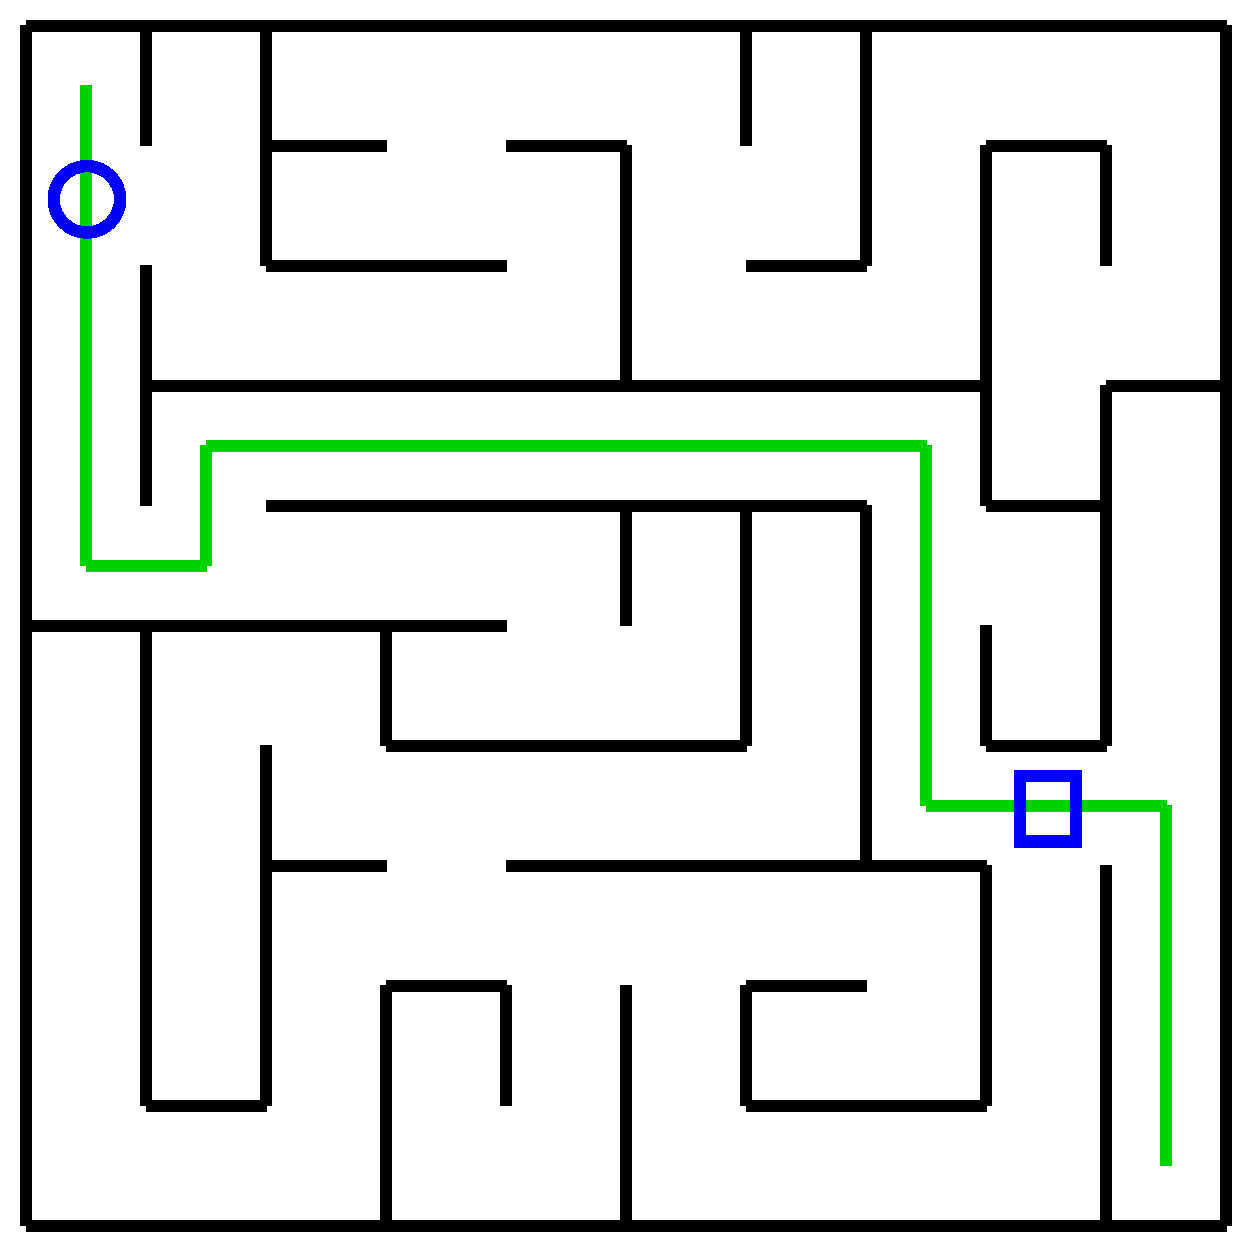
\includegraphics{SMPdesign/maze_in_way10a}}
\caption{Reason for Small Visit Percentages}
\label{fig:SMPdesign:Reason for Small Visit Percentages}
\end{figure}

\begin{figure}[tb]
\centering
\resizebox{2.2in}{!}{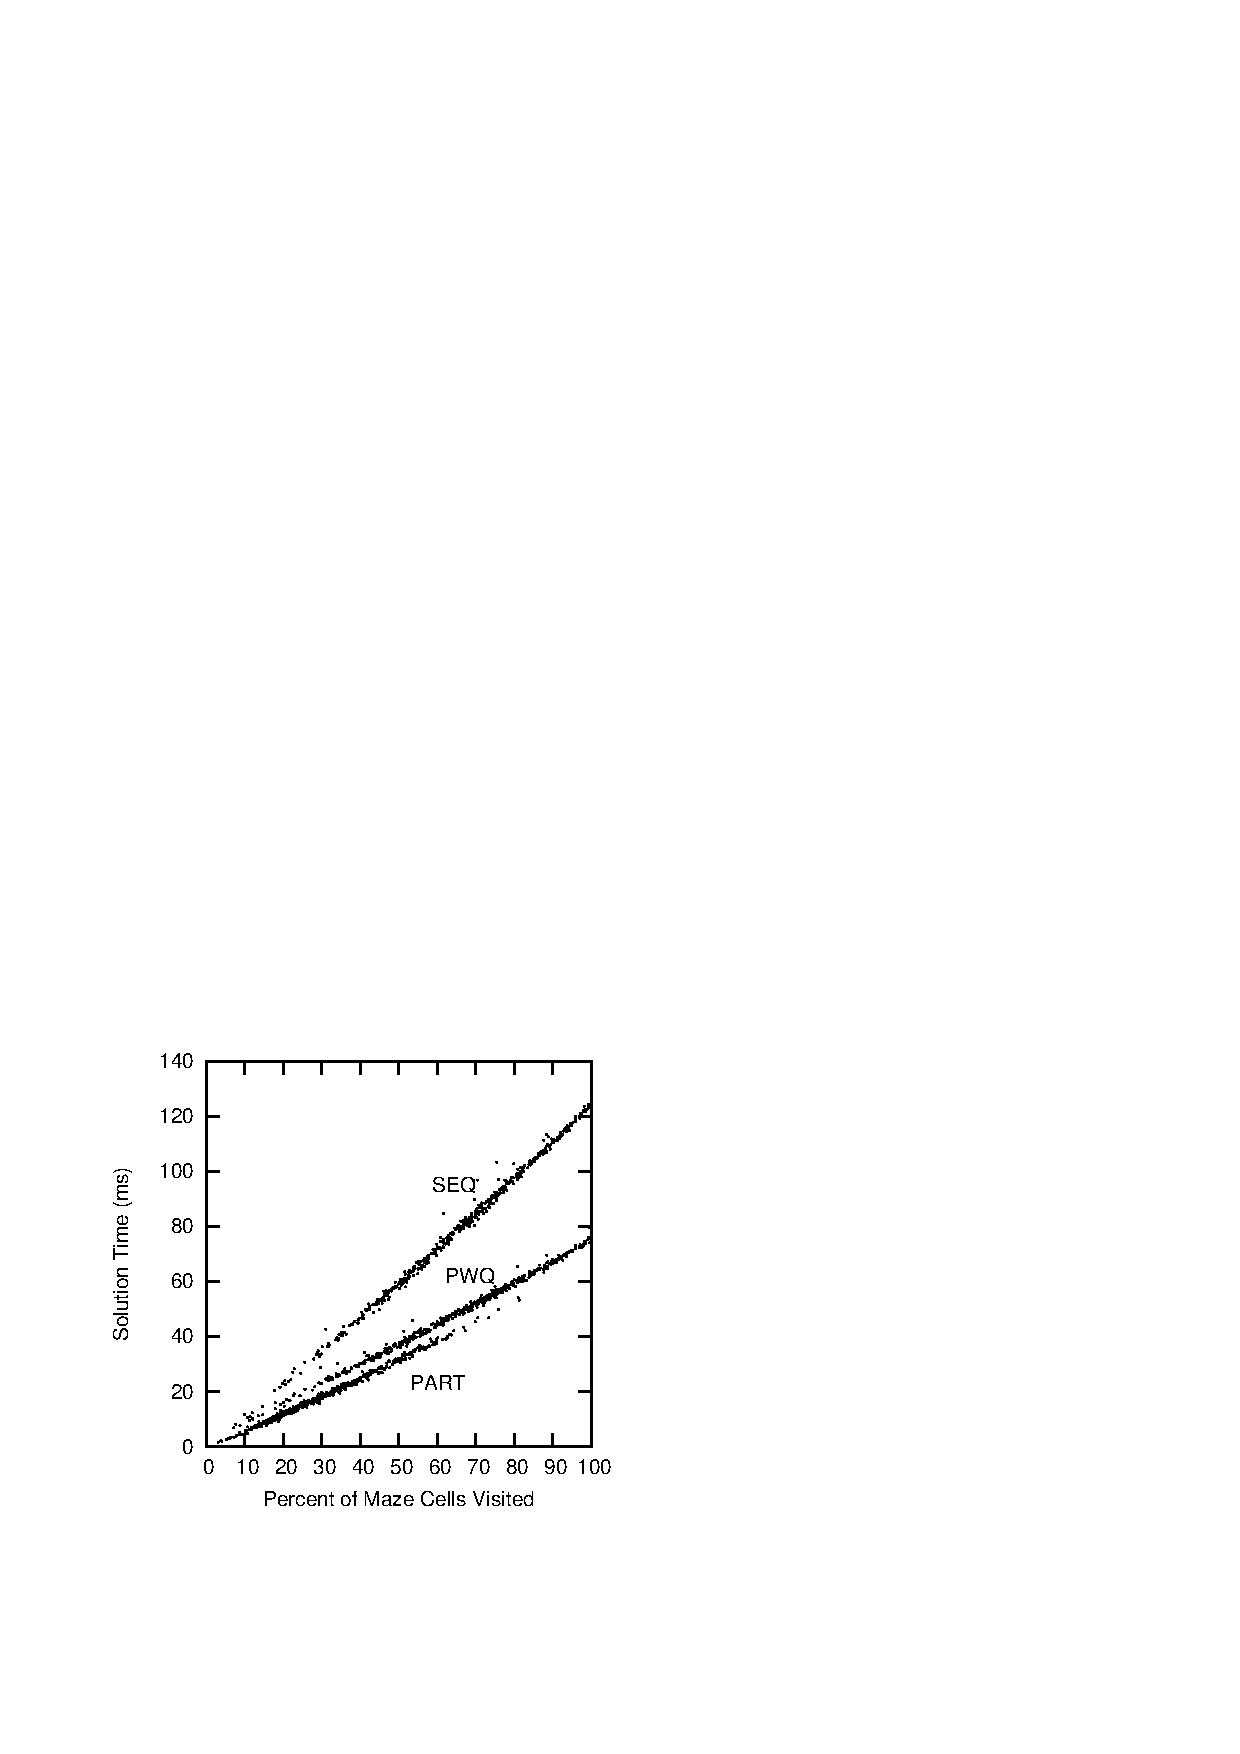
\includegraphics{SMPdesign/500-pctVms_seq_part-sct}}
\caption{Correlation Between Visit Percentage and Solution Time}
\label{fig:SMPdesign:Correlation Between Visit Percentage and Solution Time}
\end{figure}

Further investigation showed that
PART sometimes visited fewer than 2\,\% of the maze's cells,
while SEQ and PWQ never visited fewer than about 9\,\%.
The reason for this difference is shown by
Figure~\ref{fig:SMPdesign:Reason for Small Visit Percentages}.
If the thread traversing the solution from the upper left reaches
the circle, the other thread cannot reach
the upper-right portion of the maze.
Similarly, if the other thread reaches the square,
the first thread cannot reach the lower-left
portion of the maze.
Therefore, PART will likely visit a small fraction
of the non-solution-path cells.
In short, the superlinear speedups are due to threads getting in each
others' way.
This is a sharp contrast with decades of experience with
parallel programming, where workers have struggled
to keep threads \emph{out} of each others' way.

Figure~\ref{fig:SMPdesign:Correlation Between Visit Percentage and Solution Time}
confirms a strong correlation between cells visited and solution time
for all three methods.
The slope of PART's scatterplot is smaller than that of SEQ,
indicating that PART's pair of threads visits a given fraction
of the maze faster than can SEQ's single thread.
PART's scatterplot is also weighted toward small visit
percentages, confirming that PART does less total work, hence
the observed humiliating parallelism.

\begin{figure}[tb]
\centering
\resizebox{1.4in}{!}{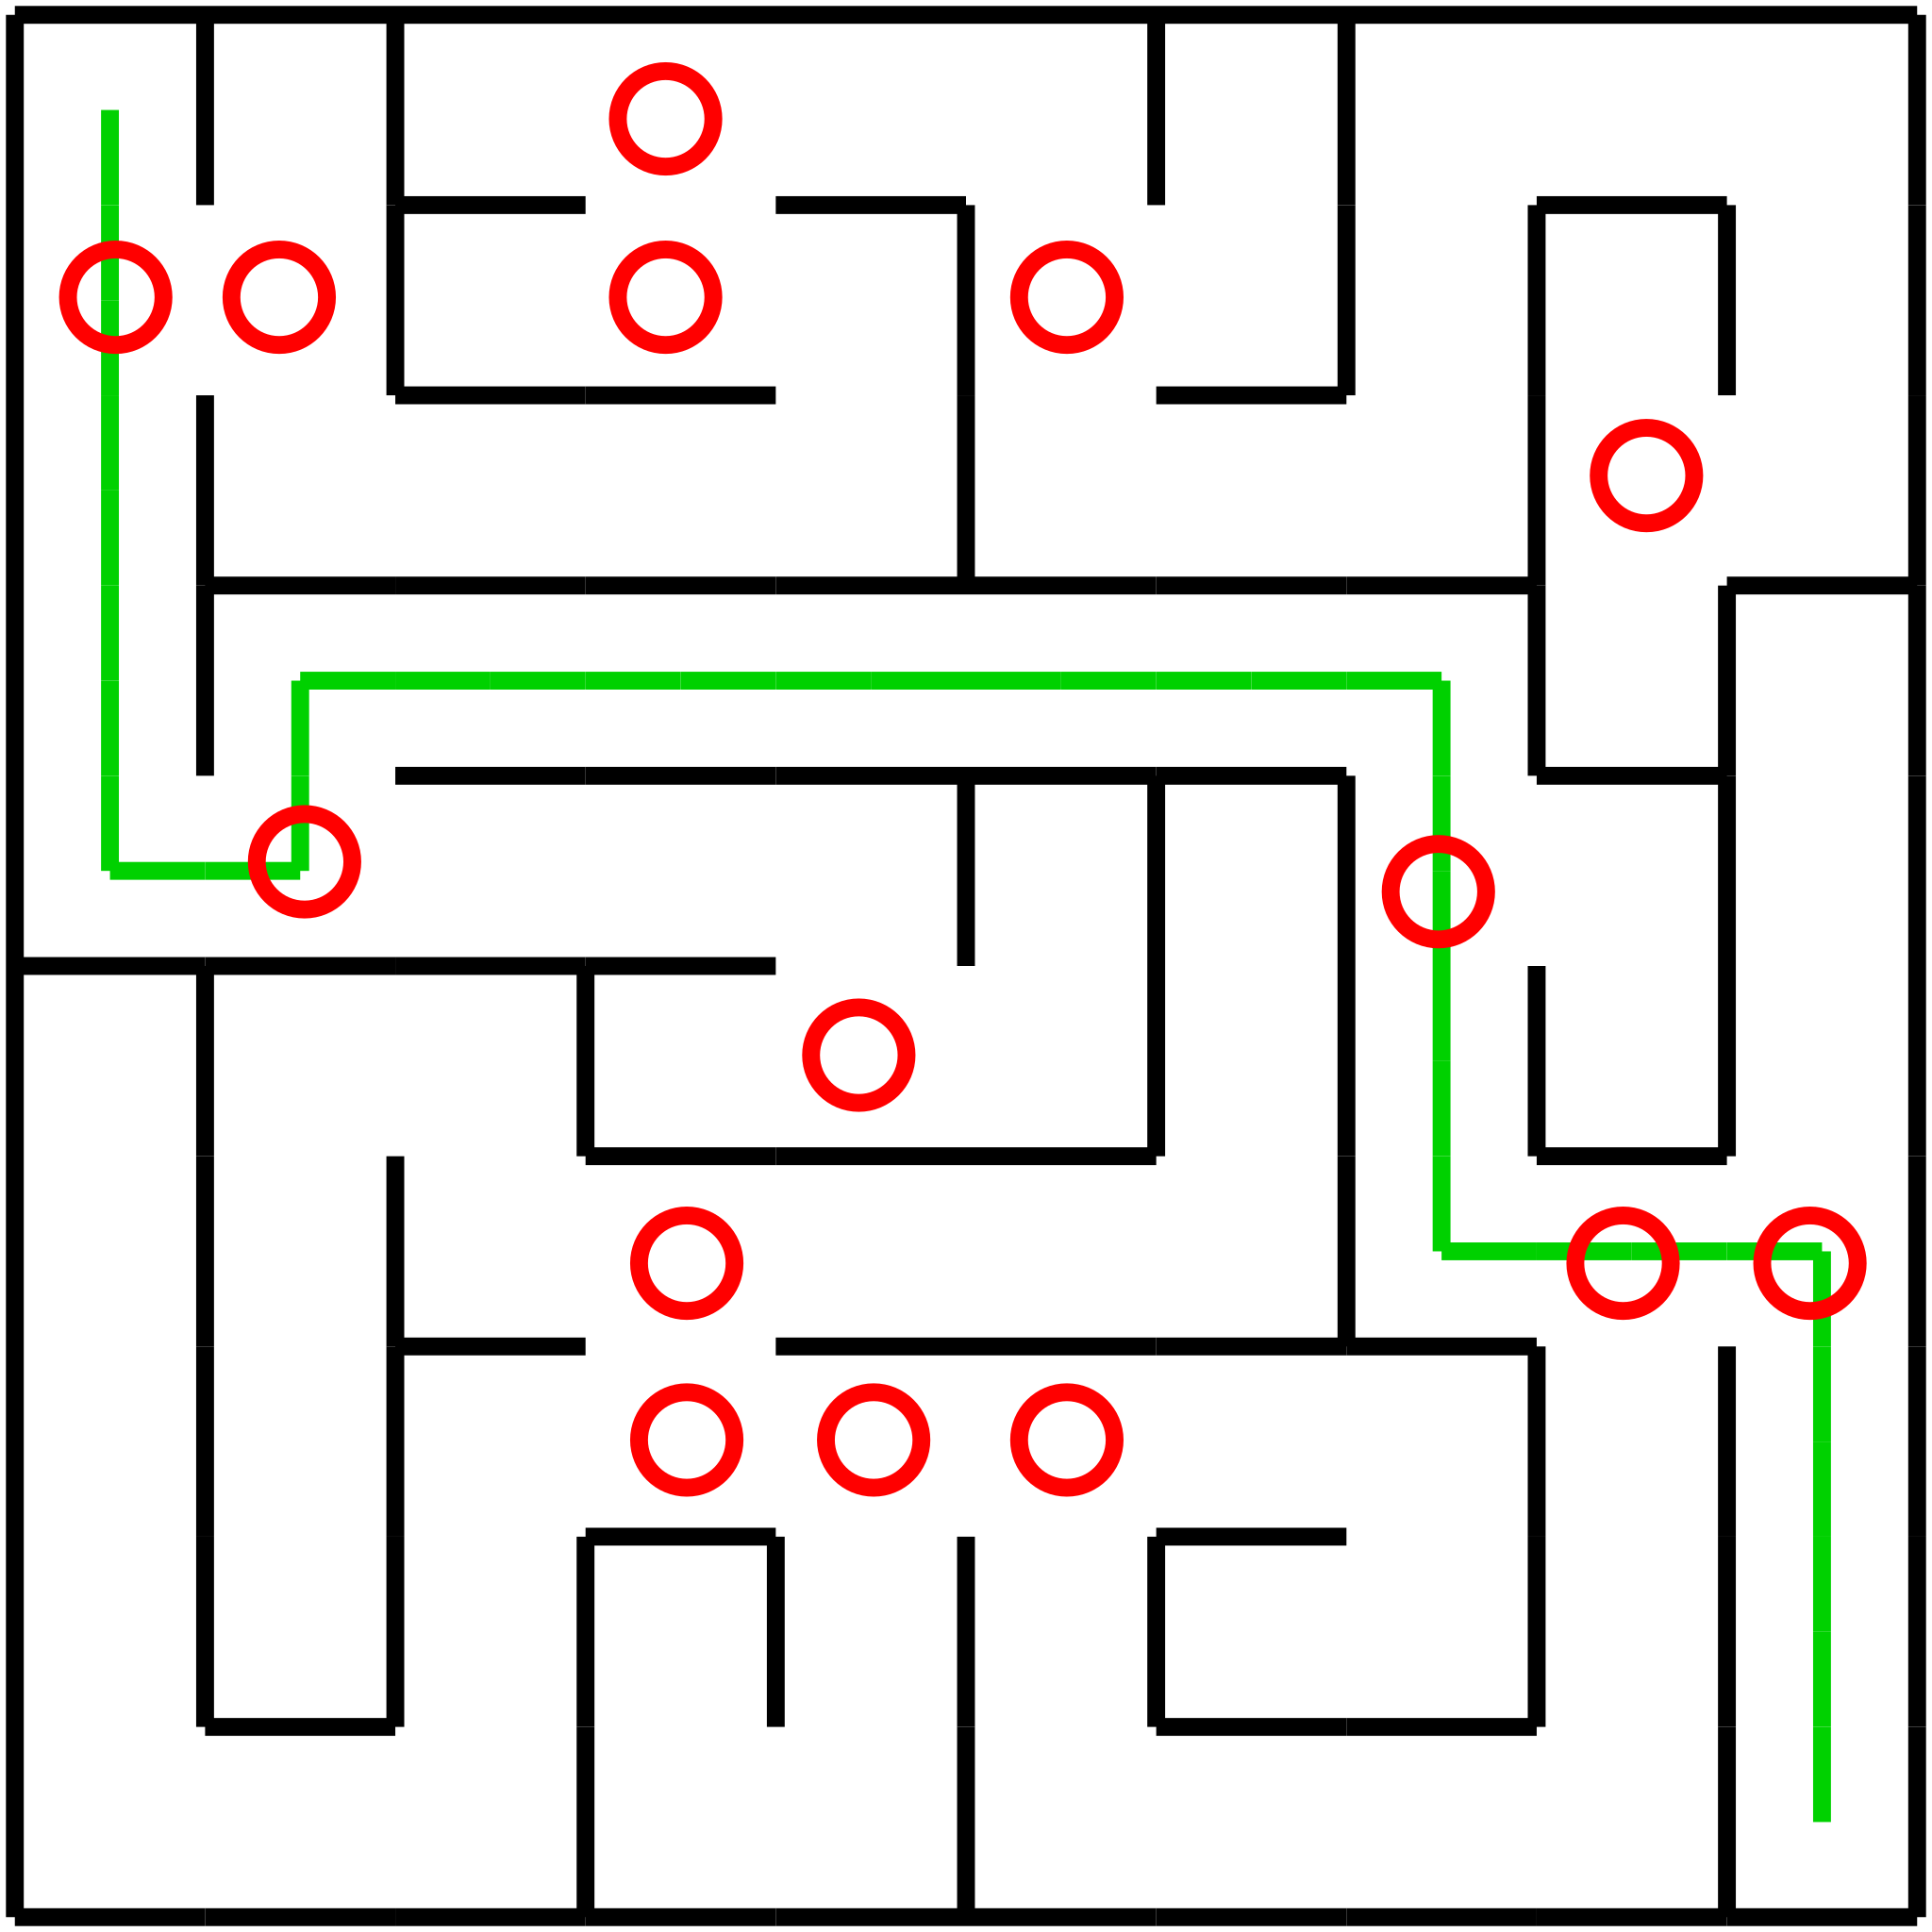
\includegraphics{SMPdesign/maze_PWQ_vs_PART}}
\caption{PWQ Potential Contention Points}
\label{fig:SMPdesign:PWQ Potential Contention Points}
\end{figure}

The fraction of cells visited by PWQ is similar to that of SEQ\@.
In addition, PWQ's solution time is greater than that of PART,
even for equal visit fractions.
The reason for this is shown in
Figure~\ref{fig:SMPdesign:PWQ Potential Contention Points}, which has a red
circle on each cell with more than two neighbors.
Each such cell can result in contention in PWQ, because
one thread can enter but two threads can exit, which hurts
performance, as noted earlier in this chapter.
In contrast, PART can incur such contention but once, namely
when the solution is located.
Of course, SEQ never contends.

\begin{figure}[tb]
\centering
\resizebox{2.2in}{!}{\includegraphics{SMPdesign/500-ms_seqVfg_part_seqO3-cdf}}
\caption{Effect of Compiler Optimization (-O3)}
\label{fig:SMPdesign:Effect of Compiler Optimization (-O3)}
\end{figure}

Although PART's speedup is impressive, we should not neglect sequential
optimizations.
Figure~\ref{fig:SMPdesign:Effect of Compiler Optimization (-O3)} shows that
SEQ, when compiled with -O3, is about twice as fast
as unoptimized PWQ, approaching the performance of unoptimized PART\@.
Compiling all three algorithms with -O3 gives results similar to
(albeit faster than) those shown in
Figure~\ref{fig:SMPdesign:CDF of SEQ/PWQ and SEQ/PART Solution-Time Ratios},
except that PWQ provides almost no speedup compared
to SEQ, in keeping with Amdahl's Law~\cite{GeneAmdahl1967AmdahlsLaw}.
However, if the goal is to double performance compared to unoptimized
SEQ, as opposed to achieving optimality, compiler
optimizations are quite attractive.

Cache alignment and padding often improves performance by reducing
false sharing.
However, for these maze-solution algorithms, aligning and padding the
maze-cell array \emph{degrades} performance by up to 42\,\% for 1000x1000 mazes.
Cache locality is more important than avoiding
false sharing, especially for large mazes.
For smaller 20-by-20 or 50-by-50 mazes, aligning and padding can produce
up to a 40\,\% performance improvement for PART,
but for these small sizes, SEQ performs better anyway because there
is insufficient time for PART to make up for the overhead of
thread creation and destruction.

In short, the partitioned parallel maze solver is an interesting example
of an algorithmic superlinear speedup.
If ``algorithmic superlinear speedup'' causes cognitive dissonance,
please proceed to the next section.

\subsection{Alternative Sequential Maze Solver}
\label{sec:SMPdesign:Alternative Sequential Maze Solver}

\begin{figure}[tb]
\centering
\resizebox{2.2in}{!}{\includegraphics{SMPdesign/500-ms_seqO3V2seqO3_fgO3_partO3-cdf}}
\caption{Partitioned Coroutines}
\label{fig:SMPdesign:Partitioned Coroutines}
\end{figure}

The presence of algorithmic superlinear speedups suggests simulating
parallelism via co-routines, for example, manually switching context
between threads on each pass through the main do-while loop in
Listing~\ref{lst:SMPdesign:Partitioned Parallel Solver Pseudocode}.
This context switching is straightforward because the context
consists only of the variables \co{c} and \co{vi}: Of the numerous
ways to achieve the effect, this is a good tradeoff between
context-switch overhead and visit percentage.
As can be seen in
Figure~\ref{fig:SMPdesign:Partitioned Coroutines},
this coroutine algorithm (COPART) is quite effective, with the performance
on one thread being within about 30\,\% of PART on two threads
(\path{maze_2seq.c}).

\subsection{Performance Comparison II}
\label{sec:SMPdesign:Performance Comparison II}

\begin{figure}[tb]
\centering
\resizebox{2.2in}{!}{\includegraphics{SMPdesign/500-ms_seqO3VfgO3_partO3-median}}
\caption{Varying Maze Size vs. SEQ}
\label{fig:SMPdesign:Varying Maze Size vs. SEQ}
\end{figure}

\begin{figure}[tb]
\centering
\resizebox{2.2in}{!}{\includegraphics{SMPdesign/500-ms_2seqO3VfgO3_partO3-median}}
\caption{Varying Maze Size vs. COPART}
\label{fig:SMPdesign:Varying Maze Size vs. COPART}
\end{figure}

Figures~\ref{fig:SMPdesign:Varying Maze Size vs. SEQ}
and~\ref{fig:SMPdesign:Varying Maze Size vs. COPART}
show the effects of varying maze size, comparing both PWQ and PART
running on two threads
against either SEQ or COPART, respectively, with 90\=/percent\-/confidence
error bars.
PART shows superlinear scalability against SEQ and modest scalability
against COPART for 100-by-100 and larger mazes.
PART exceeds theoretical energy-efficiency breakeven against COPART at roughly
the 200-by-200 maze size, given that power consumption rises as roughly
the square of the frequency for high frequencies~\cite{TrevorMudge2000Power},
so that 1.4x scaling on two threads consumes the same energy
as a single thread at equal solution speeds.
In contrast, PWQ shows poor scalability against both SEQ and COPART
unless unoptimized: Figures~\ref{fig:SMPdesign:Varying Maze Size vs. SEQ} 
and~\ref{fig:SMPdesign:Varying Maze Size vs. COPART}
were generated using -O3.

\begin{figure}[tb]
\centering
\resizebox{2.2in}{!}{\includegraphics{SMPdesign/1000-ms_2seqO3VfgO3_partO3-mean}}
\caption{Mean Speedup vs. Number of Threads, 1000x1000 Maze}
\label{fig:SMPdesign:Mean Speedup vs. Number of Threads, 1000x1000 Maze}
\end{figure}

Figure~\ref{fig:SMPdesign:Mean Speedup vs. Number of Threads, 1000x1000 Maze}
shows the performance of PWQ and PART relative to COPART\@.
For PART runs with more than two threads, the additional threads were
started evenly spaced along the diagonal connecting the starting and
ending cells.
Simplified link-state routing~\cite{BERT-87} was used to
detect early termination on PART runs with more than two threads
(the solution is flagged when
a thread is connected to both beginning and end).
PWQ performs quite poorly, but
PART hits breakeven at two threads and again at five threads, achieving
modest speedups beyond five threads.
Theoretical energy efficiency breakeven is within the 90\=/percent\-/confidence
interval for seven and eight threads.
The reasons for the peak at two threads are (1) the lower complexity
of termination detection in the two-thread case and (2) the fact that
there is a lower probability of the third and subsequent threads making
useful forward progress: Only the first two threads are guaranteed to start on
the solution line.
This disappointing performance compared to results in
Figure~\ref{fig:SMPdesign:Varying Maze Size vs. COPART}
is due to the less-tightly integrated hardware available in the
larger and older Xeon system running at 2.66\,GHz.

\subsection{Future Directions and Conclusions}
\label{sec:SMPdesign:Future Directions and Conclusions}

Much future work remains.
First, this section applied only one technique used by human maze solvers.
Others include following walls to exclude portions of the maze
and choosing internal starting points based on the
locations of previously traversed paths.
Second, different choices of
starting and ending points might favor different algorithms.
Third, although placement of the PART algorithm's
first two threads is straightforward, there are any number of
placement schemes for the remaining threads.
Optimal placement might well depend on the starting and ending points.
Fourth, study of unsolvable mazes and cyclic mazes
is likely to produce interesting results.
Fifth, the lightweight C++11 atomic operations might improve performance.
Sixth, it would be interesting to compare the speedups for
three-dimensional mazes (or of even higher-order mazes).
Finally, for mazes, humiliating parallelism indicated a
more-efficient sequential implementation using coroutines.
Do humiliatingly parallel algorithms always lead to more-efficient
sequential implementations, or are there inherently humiliatingly parallel
algorithms for which coroutine context-switch overhead overwhelms the
speedups?

This section demonstrated and analyzed parallelization of maze-solution
algorithms.
A conventional work-queue-based algorithm did well only when compiler
optimizations were disabled, suggesting that some prior results obtained
using high-level/overhead languages will be invalidated
by advances in optimization.

This section gave a clear example where approaching parallelism
as a first-class optimization technique rather than as a derivative of a
sequential algorithm paves the way for an improved sequential algorithm.
High-level design-time application of parallelism is likely to be a
fruitful field of study.
This section took the problem of solving mazes from mildly scalable
to humiliatingly parallel and back again.
It is hoped that this experience will motivate work on parallelism
as a first-class design-time whole-application optimization technique,
rather than as a grossly suboptimal after-the-fact micro-optimization
to be retrofitted into existing programs.

\section{Partitioning, Parallelism, and Optimization}
\label{sec:SMPdesign:Partitioning, Parallelism, and Optimization}
%
\epigraph{Knowledge is of no value unless you put it into practice.}
	 {\emph{Anton Chekhov}}

Most important, although this chapter has demonstrated that applying
parallelism at the design level gives excellent results, this final
section shows that this is not enough.
For search problems such as maze solution, this section has shown that
search strategy is even more important than parallel design.
Yes, for this particular type of maze, intelligently applying parallelism
identified a superior search strategy, but this sort of luck is no
substitute for a clear focus on search strategy itself.

As noted back in Section~\ref{sec:intro:Parallel Programming Goals},
parallelism is but one potential optimization of many.
A successful design needs to focus on the most important optimization.
Much though I might wish to claim otherwise, that optimization might
or might not be parallelism.

However, for the many cases where parallelism is the right optimization,
the next section covers that synchronization workhorse, locking.


% sync/sync.tex

\chapter{Locking}
\label{chp:Locking}

\section{Staying Alive}
\label{sec:sync:Staying Alive}

\subsection{Deadlock}
\label{sec:sync:Deadlock}

\subsection{Livelock}
\label{sec:sync:Livelock}

\subsection{Starvation}
\label{sec:sync:Starvation}

\subsection{Fairness}
\label{sec:sync:Fairness}

\section{Types of Locks}
\label{sec:sync:Types of Locks}

\subsection{Exclusive Locks}
\label{sec:sync:Exclusive Locks}

\subsection{Reader-Writer Locks}
\label{sec:sync:Reader-Writer Locks}

\subsection{Beyond Reader-Writer Locks}
\label{sec:sync:Beyond Reader-Writer Locks}

VAXCluster six-state locking.

\subsection{While Waiting}
\label{sec:sync:While Waiting}

Spinlocks, sleeplocks, spin-sleeplocks (maybe), conditional locking.

\section{Barriers}
\label{sec:sync:Barriers}

HPC-style barriers.

\section{The Art of Procrastination}
\label{sec:sync:The Art of Procrastination}

Completions, tasklets, work queues, data-structure queues,
brief mention of reference counters,
brief mention of RCU.

\subsection{Sleeping Safely}
\label{sec:sync:Sleeping Safely}

\section{Full Machine Stop}
\label{sec:sync:Full Machine Stop}

\section{Interrupts and Signals}
\label{sec:sync:Interrupts and Signals}

% owned/owned.tex

\chapter{Data Ownership}
\label{chp:Data Ownership}

Per-CPU and per-task/process/thread data.

Function shipping vs. data shipping.

Big question: how much local vs. global processing?  How frequent,
how expensive, ...  Better to divide or to centralize?

Relationship to map/reduce?  Message passing!

@@@ populate with problems showing benefits of coupling data ownership
with other approaches.
For example, work-stealing schedulers.
Perhaps also move memory allocation here, though its current location
is quite good.

% defer/defer.tex

\chapter{Deferred Processing}
\label{chp:defer:Deferred Processing}

\QuickQuizChapter{chp:defer:Deferred Processing}

The strategy of deferring work probably predates mankind, but only
in the last few decades have workers recognized this strategy's value
in simplifying parallel algorithms~\cite{Kung80,HMassalinPhD}.
General approaches to work deferral in parallel programming include
queuing, reference counting, and RCU.

% @@@ \input{defer/queue}
% @@@ % defer/seqlock.tex

\section{Sequence Locks}
\label{sec:defer:Sequence Locks}

\begin{figure}[tb]
\centering
\resizebox{3in}{!}{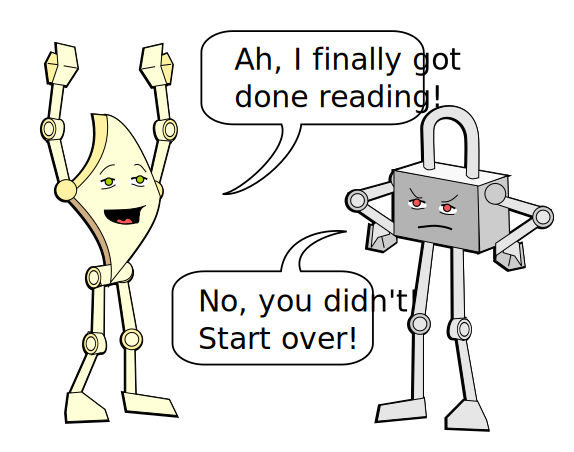
\includegraphics{cartoons/r-2014-Start-over}}
\caption{Reader And Uncooperative Sequence Lock}
\label{fig:defer:Reader And Uncooperative Sequence Lock}
\end{figure}

Sequence locks are used in the Linux kernel for read-mostly data that
must be seen in a consistent state by readers.
However, unlike reader-writer locking, readers do not exclude writers.
Instead, like hazard pointers, sequence locks force readers to
\emph{retry} an operation if they detect activity from a concurrent writer.
As can be seen from
Figure~\ref{fig:defer:Reader And Uncooperative Sequence Lock},
it is important to design code using sequence locks so that readers
very rarely need to retry.

\QuickQuiz{}
	Why isn't this sequence-lock discussion in Chapter~\ref{chp:Locking},
	you know, the one on \emph{locking}?
\QuickQuizAnswer{
	The sequence-lock mechanism is really a combination of two
	separate synchronization mechanisms, sequence counts and
	locking.
	In fact, the sequence-count mechanism is available separately
	in the Linux kernel via the
	\co{write_seqcount_begin()} and \co{write_seqcount_end()}
	primitives.

	However, the combined \co{write_seqlock()} and
	\co{write_sequnlock()} primitives are used much more heavily
	in the Linux kernel.
	More importantly, many more people will understand what you
	mean if you say ``sequence lock'' than if you say
	``sequence count''.

	So this section is entitled ``Sequence Locks'' so that people
	will understand what it is about just from the title, and
	it appears in the ``Deferred Processing'' because (1) of the
	emphasis on the ``sequence count'' aspect of ``sequence locks''
	and (2) because a ``sequence lock'' is much more than merely
	a lock.
} \QuickQuizEnd

{ \scriptsize
\begin{verbbox}
  1 do {
  2   seq = read_seqbegin(&test_seqlock);
  3   /* read-side access. */
  4 } while (read_seqretry(&test_seqlock, seq));
\end{verbbox}
}
\begin{figure}[bp]
\centering
\theverbbox
\caption{Sequence-Locking Reader}
\label{fig:defer:Sequence-Locking Reader}
\end{figure}

{ \scriptsize
\begin{verbbox}
  1 write_seqlock(&test_seqlock);
  2 /* Update */
  3 write_sequnlock(&test_seqlock);
\end{verbbox}
}
\begin{figure}[bp]
\centering
\theverbbox
\caption{Sequence-Locking Writer}
\label{fig:defer:Sequence-Locking Writer}
\end{figure}

The key component of sequence locking is the sequence number, which has
an even value in the absence of updaters and an odd value if there
is an update in progress.
Readers can then snapshot the value before and after each access.
If either snapshot has an odd value, or if the two snapshots differ,
there has been a concurrent update, and the reader must discard
the results of the access and then retry it.
Readers therefore use the \co{read_seqbegin()} and \co{read_seqretry()}
functions shown in Figure~\ref{fig:defer:Sequence-Locking Reader}
when accessing data protected by a sequence lock.
Writers must increment the value before and after each update,
and only one writer is permitted at a given time.
Writers therefore use the \co{write_seqlock()} and \co{write_sequnlock()}
functions shown in Figure~\ref{fig:defer:Sequence-Locking Writer}
when updating data protected by a sequence lock.

As a result, sequence-lock-protected data can have an arbitrarily
large number of concurrent readers, but only one writer at a time.
Sequence locking is used in the Linux kernel to protect calibration
quantities used for timekeeping.
It is also used in pathname traversal to detect concurrent rename operations.

{ \scriptsize
\begin{verbbox}
 1  typedef struct {
 2    unsigned long seq;
 3    spinlock_t lock;
 4  } seqlock_t;
 5
 6  static void seqlock_init(seqlock_t *slp)
 7  {
 8    slp->seq = 0;
 9    spin_lock_init(&slp->lock);
10  }
11
12  static unsigned long read_seqbegin(seqlock_t *slp)
13  {
14    unsigned long s;
15
16    s = ACCESS_ONCE(slp->seq);
17    smp_mb();
18    return s & ~0x1UL;
19  }
20
21  static int read_seqretry(seqlock_t *slp,
22                           unsigned long oldseq)
23  {
24    unsigned long s;
25
26    smp_mb();
27    s = ACCESS_ONCE(slp->seq);
28    return s != oldseq;
29  }
30
31  static void write_seqlock(seqlock_t *slp)
32  {
33    spin_lock(&slp->lock);
34    ++slp->seq;
35    smp_mb();
36  }
37
38  static void write_sequnlock(seqlock_t *slp)
39  {
40    smp_mb();
41    ++slp->seq;
42    spin_unlock(&slp->lock);
43  }
\end{verbbox}
}
\begin{figure}[tb]
\centering
\theverbbox
\caption{Sequence-Locking Implementation}
\label{fig:defer:Sequence-Locking Implementation}
\end{figure}

A simple implementation of sequence locks is shown in
Figure~\ref{fig:defer:Sequence-Locking Implementation}
(\path{seqlock.h}).
The \co{seqlock_t} data structure is shown on lines~1-4, and contains
the sequence number along with a lock to serialize writers.
Lines~6-10 show \co{seqlock_init()}, which, as the name indicates,
initializes a \co{seqlock_t}.

Lines~12-19 show \co{read_seqbegin()}, which begins a sequence-lock
read-side critical section.
Line~16 takes a snapshot of the sequence counter, and line~17 orders
this snapshot operation before the caller's critical section.
Finally, line~18 returns the value of the snapshot (with the least-significant
bit cleared), which the caller
will pass to a later call to \co{read_seqretry()}.

\QuickQuiz{}
	Why not have \co{read_seqbegin()} in
	Figure~\ref{fig:defer:Sequence-Locking Implementation}
	check for the low-order bit being set, and retry
	internally, rather than allowing a doomed read to start?
\QuickQuizAnswer{
	That would be a legitimate implementation.
	However, if the workload is read-mostly, it would likely
	increase the overhead of the common-case successful read,
	which could be counter-productive.
	However, given a sufficiently large fraction of updates
	and sufficiently high-overhead readers, having the
	check internal to \co{read_seqbegin()} might be preferable.
} \QuickQuizEnd

Lines~21-29 show \co{read_seqretry()}, which returns true if there
were no writers present since the time of the corresponding
call to \co{read_seqbegin()}.
Line~26 orders the caller's prior critical section before line~27's
fetch of the new snapshot of the sequence counter.
Finally, line~28 checks that the sequence counter has not changed,
in other words, that there has been no writer, and returns true if so.

\QuickQuiz{}
	Why is the \co{smp_mb()} on line~26 of
	Figure~\ref{fig:defer:Sequence-Locking Implementation}
	needed?
\QuickQuizAnswer{
	If it was omitted, both the compiler and the CPU would be
	within their rights to move the critical section preceding
	the call to \co{read_seqretry()} down below this function.
	This would prevent the sequence lock from protecting the
	critical section.
	The \co{smp_mb()} primitive prevents such reordering.
} \QuickQuizEnd

\QuickQuiz{}
	Can't weaker memory barriers be used in the code in
	Figure~\ref{fig:defer:Sequence-Locking Implementation}?
\QuickQuizAnswer{
	In older versions of the Linux kernel, no.

	In very new versions of the Linux kernel, line~16 could use
	\co{smp_load_acquire()} instead of \co{ACCESS_ONCE()}, which
	in turn would allow the \co{smp_mb()} on line~17 to be dropped.
	Similarly, line~41 could use an \co{smp_store_release()}, for
	example, as follows: \\
	\co{smp_store_release(&slp->seq, ACCESS_ONCE(slp->seq) + 1);} \\
	This would allow the \co{smp_mb()} on line~40 to be dropped.
} \QuickQuizEnd

\QuickQuiz{}
	What prevents sequence-locking updaters from starving readers?
\QuickQuizAnswer{
	Nothing.
	This is one of the weaknesses of sequence locking, and as a
	result, you should use sequence locking only in read-mostly
	situations.
	Unless of course read-side starvation is acceptable in your
	situation, in which case, go wild with the sequence-locking updates!
} \QuickQuizEnd

Lines~31-36 show \co{write_seqlock()}, which simply acquires the lock,
increments the sequence number, and executes a memory barrier to ensure
that this increment is ordered before the caller's critical section.
Lines~38-43 show \co{write_sequnlock()}, which executes a memory barrier
to ensure that the caller's critical section is ordered before the
increment of the sequence number on line~44, then releases the lock.

\QuickQuiz{}
	What if something else serializes writers, so that the lock
	is not needed?
\QuickQuizAnswer{
	In this case, the \co{->lock} field could be omitted, as it
	is in \co{seqcount_t} in the Linux kernel.
} \QuickQuizEnd

\QuickQuiz{}
	Why isn't \co{seq} on line~2 of
	Figure~\ref{fig:defer:Sequence-Locking Implementation}
	\co{unsigned} rather than \co{unsigned long}?
	After all, if \co{unsigned} is good enough for the Linux
	kernel, shouldn't it be good enough for everyone?
\QuickQuizAnswer{
	Not at all.
	The Linux kernel has a number of special attributes that allow
	it to ignore the following sequence of events:
	\begin{enumerate}
	\item	Thread~0 executes \co{read_seqbegin()}, picking up
		\co{->seq} in line~16, noting that the value is even,
		and thus returning to the caller.
	\item	Thread~0 starts executing its read-side critical section,
		but is then preempted for a long time.
	\item	Other threads repeatedly invoke \co{write_seqlock()} and
		\co{write_sequnlock()}, until the value of \co{->seq}
		overflows back to the value that Thread~0 fetched.
	\item	Thread~0 resumes execution, completing its read-side
		critical section with inconsistent data.
	\item	Thread~0 invokes \co{read_seqretry()}, which incorrectly
		concludes that Thread~0 has seen a consistent view of
		the data protected by the sequence lock.
	\end{enumerate}

	The Linux kernel uses sequence locking for things that are
	updated rarely, with time-of-day information being a case
	in point.
	This information is updated at most once per millisecond,
	so that seven weeks would be required to overflow the counter.
	If a kernel thread was preempted for seven weeks, the Linux
	kernel's soft-lockup code would be emitting warnings every two
	minutes for that entire time.

	In contrast, with a 64-bit counter, more than five centuries
	would be required to overflow, even given an update every
	\emph{nano}second.
	Therefore, this implementation uses a type for \co{->seq}
	that is 64 bits on 64-bit systems.
} \QuickQuizEnd

{ \scriptsize
\begin{verbbox}
 1 struct route_entry {
 2   struct route_entry *re_next;
 3   unsigned long addr;
 4   unsigned long iface;
 5   int re_freed;
 6 };
 7 struct route_entry route_list;
 8 DEFINE_SEQ_LOCK(sl);
 9
10 unsigned long route_lookup(unsigned long addr)
11 {
12   struct route_entry *rep;
13   struct route_entry **repp;
14   unsigned long ret;
15   unsigned long s;
16
17 retry:
18   s = read_seqbegin(&sl);
19   repp = &route_list.re_next;
20   do {
21     rep = ACCESS_ONCE(*repp);
22     if (rep == NULL) {
23       if (read_seqretry(&sl, s))
24         goto retry;
25       return ULONG_MAX;
26     }
27     repp = &rep->re_next;
28   } while (rep->addr != addr);
29   if (ACCESS_ONCE(rep->re_freed))
30     abort();
31   ret = rep->iface;
32   if (read_seqretry(&sl, s))
33     goto retry;
34   return ret;
35 }
\end{verbbox}
}
\begin{figure}[tbp]
\centering
\theverbbox
\caption{Sequence-Locked Pre-BSD Routing Table Lookup (BUGGY!!!)}
\label{fig:defer:Sequence-Locked Pre-BSD Routing Table Lookup}
\end{figure}

{ \scriptsize
\begin{verbbox}
 1 int route_add(unsigned long addr,
 2               unsigned long interface)
 3 {
 4   struct route_entry *rep;
 5
 6   rep = malloc(sizeof(*rep));
 7   if (!rep)
 8     return -ENOMEM;
 9   rep->addr = addr;
10   rep->iface = interface;
11   rep->re_freed = 0;
12   write_seqlock(&sl);
13   rep->re_next = route_list.re_next;
14   route_list.re_next = rep;
15   write_sequnlock(&sl);
16   return 0;
17 }
18
19 int route_del(unsigned long addr)
20 {
21   struct route_entry *rep;
22   struct route_entry **repp;
23
24   write_seqlock(&sl);
25   repp = &route_list.re_next;
26   for (;;) {
27     rep = *repp;
28     if (rep == NULL)
29       break;
30     if (rep->addr == addr) {
31       *repp = rep->re_next;
32       write_sequnlock(&sl);
33       smp_mb();
34       rep->re_freed = 1;
35       free(rep);
36       return 0;
37     }
38     repp = &rep->re_next;
39   }
40   write_sequnlock(&sl);
41   return -ENOENT;
42 }
\end{verbbox}
}
\begin{figure}[tbp]
\centering
\theverbbox
\caption{Sequence-Locked Pre-BSD Routing Table Add/Delete (BUGGY!!!)}
\label{fig:defer:Sequence-Locked Pre-BSD Routing Table Add/Delete}
\end{figure}

So what happens when sequence locking is applied to the Pre-BSD
routing table?
Figure~\ref{fig:defer:Sequence-Locked Pre-BSD Routing Table Lookup}
shows the data structures and \co{route_lookup()}, and
Figure~\ref{fig:defer:Sequence-Locked Pre-BSD Routing Table Add/Delete}
shows \co{route_add()} and \co{route_del()} (\path{route_seqlock.c}).
This implementation is once again similar to its counterparts in earlier
sections, so only the differences will be highlighted.

In
Figure~\ref{fig:defer:Sequence-Locked Pre-BSD Routing Table Lookup},
line~5 adds \co{->re_freed}, which is checked on lines~29 and~30.
Line~8 adds a sequence lock, which is used by \co{route_lookup()}
on lines~18, 23, and~32, with lines~24 and~33 branching back to
the \co{retry} label on line~17.
The effect is to retry any lookup that runs concurrently with an update.

In
Figure~\ref{fig:defer:Sequence-Locked Pre-BSD Routing Table Add/Delete},
lines~12, 15, 24, and~40 acquire and release the sequence lock,
while lines~11, 33, and~44 handle \co{->re_freed}.
This implementation is therefore quite straightforward.

\begin{figure}[tb]
\centering
\resizebox{2.5in}{!}{\includegraphics{CodeSamples/defer/perf-seqlock}}
\caption{Pre-BSD Routing Table Protected by Sequence Locking}
\label{fig:defer:Pre-BSD Routing Table Protected by Sequence Locking}
\end{figure}

It also performs better on the read-only workload, as can be seen in
Figure~\ref{fig:defer:Pre-BSD Routing Table Protected by Sequence Locking},
though its performance is still far from ideal.

Unfortunately, it also suffers use-after-free failures.
The problem is that the reader might encounter a segmentation violation
due to accessing an already-freed structure before it comes to the
\co{read_seqretry()}.

\QuickQuiz{}
	Can this bug be fixed?
	In other words, can you use sequence locks as the \emph{only}
	synchronization mechanism protecting a linked list supporting
	concurrent addition, deletion, and lookup?
\QuickQuizAnswer{
	One trivial way of accomplishing this is to surround all
	accesses, including the read-only accesses, with
	\co{write_seqlock()} and \co{write_sequnlock()}.
	Of course, this solution also prohibits all read-side
	parallelism, resulting in massive lock contention,
	and furthermore could just as easily be implemented
	using simple locking.

	If you do come up with a solution that uses \co{read_seqbegin()}
	and \co{read_seqretry()} to protect read-side accesses, make
	sure that you correctly handle the following sequence of events:

	\begin{enumerate}
	\item	CPU~0 is traversing the linked list, and picks up a pointer
		to list element~A.
	\item	CPU~1 removes element~A from the list and frees it.
	\item	CPU~2 allocates an unrelated data structure, and gets
		the memory formerly occupied by element~A.
		In this unrelated data structure, the memory previously
		used for element~A's \co{->next} pointer is now occupied
		by a floating-point number.
	\item	CPU~0 picks up what used to be element~A's \co{->next}
		pointer, gets random bits, and therefore gets a
		segmentation fault.
	\end{enumerate}

	One way to protect against this sort of problem requires use
	of ``type-safe memory'', which will be discussed in
	Section~\ref{sec:defer:RCU is a Way of Providing Type-Safe Memory}.
	But in that case, you would be using some other synchronization
	mechanism in addition to sequence locks!
} \QuickQuizEnd

Both the read-side and write-side critical sections of a sequence lock
can be thought of as transactions, and sequence locking therefore
can be thought of as a limited form of transactional memory, which
will be discussed in Section~\ref{sec:future:Transactional Memory}.
The limitations of sequence locking are: (1)~Sequence locking restricts
updates and (2)~sequence locking does not permit traversal of pointers
to objects that might be freed by updaters.
These limitations are of course overcome by transactional memory, but
can also be overcome by combining other synchronization primitives
with sequence locking.

Sequence locks allow writers to defer readers, but not vice versa.
This can result in unfairness and even starvation
in writer-heavy workloads.
On the other hand, in the absence of writers, sequence-lock readers are
reasonably fast and scale linearly.
It is only human to want the best of both worlds: fast readers without
the possibility of read-side failure, let alone starvation.
In addition, it would also be nice to overcome sequence locking's limitations
with pointers.
The following section presents a synchronization mechanism with exactly
these properties.

% defer/refcnt.tex
% mainfile: ../perfbook.tex
% SPDX-License-Identifier: CC-BY-SA-3.0

\section{Reference Counting}
\label{sec:defer:Reference Counting}
%
\epigraph{I am never letting you go!}{Unknown}

\begin{listing}[tbp]
\input{CodeSamples/defer/route_refcnt@lookup.fcv}
\caption{Reference-Counted Pre-BSD Routing Table Lookup (BUGGY!!!)}
\label{lst:defer:Reference-Counted Pre-BSD Routing Table Lookup}
\end{listing}

\begin{listing}[tbp]
\input{CodeSamples/defer/route_refcnt@add_del.fcv}
\caption{Reference-Counted Pre-BSD Routing Table Add\slash Delete (BUGGY!!!)}
\label{lst:defer:Reference-Counted Pre-BSD Routing Table Add/Delete}
\end{listing}

Reference counting tracks the number of references to a given object in
order to prevent that object from being prematurely freed.
As such, it has a long and honorable history of use dating back to
at least the early
1960s~\cite{Weizenbaum:1963:SLP:367593.367617}.\footnote{
	Weizenbaum discusses reference counting as if it was already
	well-known, so it likely dates back to the 1950s and perhaps
	even to the 1940s.
	And perhaps even further.
	People repairing and maintaining large dangerous machines have long
	used a mechanical reference-counting technique implemented via
	padlocks.
	Before entering the machine, each worker locks a padlock onto
	the machine's on/off switch, thus preventing the machine from
	being powered on while that worker is inside.}
Reference counting is thus an excellent candidate for a concurrent
implementation of Pre-BSD routing.

To that end,
Listing~\ref{lst:defer:Reference-Counted Pre-BSD Routing Table Lookup}
shows data structures and the \co{route_lookup()} function and
Listing~\ref{lst:defer:Reference-Counted Pre-BSD Routing Table Add/Delete}
shows the \co{route_add()} and \co{route_del()} functions
(all at \path{route_refcnt.c}).
Since these algorithms are quite similar to the sequential algorithm
shown in
Listing~\ref{lst:defer:Sequential Pre-BSD Routing Table},
only the differences will be discussed.

\begin{lineref}[ln:defer:route_refcnt:lookup:entry]
Starting with
Listing~\ref{lst:defer:Reference-Counted Pre-BSD Routing Table Lookup},
line~\lnref{refcnt} adds the actual reference counter,
line~\lnref{freed} adds a \co{->re_freed}
use-after-free check field,
line~\lnref{routelock} adds the \co{routelock} that will
be used to synchronize concurrent updates,
\end{lineref}
\begin{lineref}[ln:defer:route_refcnt:lookup:re_free]
and lines~\lnref{b}-\lnref{e} add \co{re_free()}, which sets
\co{->re_freed}, enabling \co{route_lookup()} to check for
use-after-free bugs.
\end{lineref}
\begin{lineref}[ln:defer:route_refcnt:lookup:lookup]
In \co{route_lookup()} itself,
lines~\lnref{relprev:b}-\lnref{relprev:e} release the reference
count of the prior element and free it if the count becomes zero,
and lines~\lnref{acq:b}-\lnref{acq:e} acquire a reference on the new element,
with lines~\lnref{check_uaf}
and~\lnref{abort} performing the use-after-free check.
\end{lineref}

\QuickQuiz{}
	Why bother with a use-after-free check?
\QuickQuizAnswer{
	To greatly increase the probability of finding bugs.
	A small torture-test program
	(\path{routetorture.h}) that allocates and frees only
	one type of structure can tolerate a surprisingly
	large amount of use-after-free misbehavior.
	See Figure~\ref{fig:debugging:Number of Tests Required for 99 Percent Confidence Given Failure Rate}
	on page~\pageref{fig:debugging:Number of Tests Required for 99 Percent Confidence Given Failure Rate}
	and the related discussion in
	Section~\ref{sec:debugging:Hunting Heisenbugs}
	starting on
	page~\pageref{sec:debugging:Hunting Heisenbugs}
	for more on the importance
	of increasing the probability of finding bugs.
} \QuickQuizEnd

\begin{lineref}[ln:defer:route_refcnt:add_del]
In Listing~\ref{lst:defer:Reference-Counted Pre-BSD Routing Table Add/Delete},
lines~\lnref{acq1}, \lnref{rel1}, \lnref{acq2}, \lnref{rel2},
and~\lnref{rel3} introduce locking to synchronize
concurrent updates.
Line~\lnref{init:freed} initializes the \co{->re_freed} use-after-free-check field,
and finally lines~\lnref{re_free:b}-\lnref{re_free:e} invoke
\co{re_free()} if the new value of
the reference count is zero.
\end{lineref}

\QuickQuiz{}
	Why doesn't \co{route_del()} in
	Listing~\ref{lst:defer:Reference-Counted Pre-BSD Routing Table Add/Delete}
	use reference counts to
	protect the traversal to the element to be freed?
\QuickQuizAnswer{
	Because the traversal is already protected by the lock, so
	no additional protection is required.
} \QuickQuizEnd

\begin{figure}[tb]
\centering
\resizebox{2.5in}{!}{\includegraphics{CodeSamples/defer/perf-refcnt}}
\caption{Pre-BSD Routing Table Protected by Reference Counting}
\label{fig:defer:Pre-BSD Routing Table Protected by Reference Counting}
\end{figure}

Figure~\ref{fig:defer:Pre-BSD Routing Table Protected by Reference Counting}
shows the performance and scalability of reference counting on a
read-only workload with a ten-element list running on a
single-socket four-core hyperthreaded 2.5\,GHz x86 system.
The ``ideal'' trace was generated by running the sequential code shown in
Listing~\ref{lst:defer:Sequential Pre-BSD Routing Table},
which works only because this is a read-only workload.
The reference-counting performance is abysmal and its scalability even
more so, with the ``refcnt'' trace dropping down onto the x-axis.
This should be no surprise in view of
Chapter~\ref{chp:Hardware and its Habits}:
The reference-count acquisitions and releases have added frequent
shared-memory writes to an otherwise read-only workload, thus
incurring severe retribution from the laws of physics.
As well it should, given that all the wishful thinking in the world
is not going to increase the speed of light or decrease the size of
the atoms used in modern digital electronics.

\QuickQuiz{}
	Why the stairsteps in the ``ideal'' line in
	Figure~\ref{fig:defer:Pre-BSD Routing Table Protected by Reference Counting}?
	Shouldn't it be a straight line?
\QuickQuizAnswer{
	The stair-steps are due to hyperthreading.
	On this particular system, the hardware threads in a given
	core have consecutive CPU numbers.
	In addition, this particular pointer-following
	low-cache-miss-rate workload seems
	to allow a single hardware thread to consume most of the
	relevant resources within its core.
	Workloads featuring heavier computational loads should be
	expected to gain greater benefit from each core's second
	hardware thread.
} \QuickQuizEnd

\QuickQuiz{}
	Why, in these modern times, does
	Figure~\ref{fig:defer:Pre-BSD Routing Table Protected by Reference Counting}
	only go up to 8 CPUs???
\QuickQuizAnswer{
	Given the horrible scalability of reference counting, who needs
	more than eight CPUs?
	Four CPUs would have sufficed to make the point!
	However, people wanting more CPUs are urged to refer to
	Chapter~\ref{chp:Data Structures}.
} \QuickQuizEnd

But it gets worse.

Running multiple updater threads repeatedly invoking
\co{route_add()} and \co{route_del()} will quickly encounter the
\co{abort()} statement on
line~\ref{ln:defer:route_refcnt:lookup:lookup:abort} of
Listing~\ref{lst:defer:Reference-Counted Pre-BSD Routing Table Lookup},
which indicates a use-after-free bug.
This in turn means that the reference counts are not only profoundly
degrading scalability and performance, but also failing to provide
the needed protection.

One sequence of events leading to the use-after-free bug is as follows,
given the list shown in
Figure~\ref{fig:defer:Pre-BSD Packet Routing List}:

\begin{lineref}[ln:defer:route_refcnt:lookup]
\begin{enumerate}
\item	Thread~A looks up address~42, reaching
	line~\lnref{lookup:check_NULL} of
	\co{route_lookup()} in
	Listing~\ref{lst:defer:Reference-Counted Pre-BSD Routing Table Lookup}.
	In other words, Thread~A has a pointer to the first element,
	but has not yet acquired a reference to it.
\item	Thread~B invokes \co{route_del()} in
	Listing~\ref{lst:defer:Reference-Counted Pre-BSD Routing Table Add/Delete}
	to delete the route entry for address~42.
	It completes successfully, and because this entry's \co{->re_refcnt}
	field was equal to the value one, it invokes
	\co{re_free()} to set the \co{->re_freed} field and to free the entry.
\item	Thread~A continues execution of \co{route_lookup()}.
	Its \co{rep} pointer is non-\co{NULL}, but
	line~\lnref{lookup:check_uaf} sees that
	its \co{->re_freed} field is non-zero,
        so line~\lnref{lookup:abort} invokes
	\co{abort()}.
\end{enumerate}
\end{lineref}

The problem is that the reference count is located in the object
to be protected, but that means that there is no protection during
the instant in time when the reference count itself is being acquired!
This is the reference-counting counterpart of a locking issue noted
by Gamsa et al.~\cite{Gamsa99}.
One could imagine using a global lock or reference count to protect
the per-route-entry reference-count acquisition, but this would
result in severe contention issues.
Although algorithms exist that allow safe reference-count acquisition
in a concurrent environment~\cite{Valois95a}, they are not only extremely
complex and error-prone~\cite{MagedMichael95a}, but also provide
terrible performance and scalability~\cite{ThomasEHart2007a}.

In short, concurrency has most definitely reduced the usefulness
of reference counting!

\QuickQuiz{}
	If concurrency has ``most definitely reduced the usefulness
	of reference counting'', why are there so many reference
	counters in the Linux kernel?
\QuickQuizAnswer{
	That sentence did say ``reduced the usefulness'', not
	``eliminated the usefulness'', now didn't it?

	Please see
	Section~\ref{sec:together:Refurbish Reference Counting},
	which discusses some of the techniques that the Linux kernel
	uses to take advantage of reference counting in a highly
	concurrent environment.
} \QuickQuizEnd

That said, sometimes it is necessary to look at a problem in an
entirely different way in order to successfully solve it.
The next section describes what could be thought of as an
inside-out reference count that provides decent performance
and scalability.

% rcu.tex
% SPDX-License-Identifier: CC-BY-SA-3.0

\section{Read-Copy Update (RCU)}
\label{sec:defer:Read-Copy Update (RCU)}

All of the mechanisms discussed in the preceding sections
used one of a number of approaches to defer specific actions
until they may be carried out safely.
The reference counters discussed in
Section~\ref{sec:defer:Reference Counting}
use explicit counters to defer actions that could disturb readers,
which results in read-side contention and thus poor scalability.
The hazard pointers covered by
Section~\ref{sec:defer:Hazard Pointers}
uses implicit counters in the guise of per-thread lists of pointer.
This avoids read-side contention, but requires
full memory barriers in read-side primitives.
The sequence lock presented in
Section~\ref{sec:defer:Sequence Locks}
also avoids read-side contention, but does not protect pointer
traversals and, like hazard pointers, requires full memory barriers
in read-side primitives.
These schemes' shortcomings raise the question of
whether it is possible to do better.

This section introduces \emph{read-copy update} (RCU), which provides
an API that allows delays to be identified in the source code,
rather than as expensive updates to shared data.
The remainder of this
section examines RCU from a number of different perspectives.
Section~\ref{sec:defer:Introduction to RCU} provides the classic
introduction to RCU,
Section~\ref{sec:defer:RCU Fundamentals} covers fundamental RCU
concepts,
Section~\ref{sec:defer:RCU Usage} introduces some common uses of RCU,
Section~\ref{sec:defer:RCU Linux-Kernel API} presents the Linux-kernel
API,
Section~\ref{sec:defer:``Toy'' RCU Implementations} covers a sequence
of ``toy'' implementations of user-level RCU,
and finally
Section~\ref{sec:defer:RCU Exercises} provides some RCU exercises.

% defer/rcuintro.tex
% mainfile: ../perfbook.tex
% SPDX-License-Identifier: CC-BY-SA-3.0

\subsection{Introduction to RCU}
\label{sec:defer:Introduction to RCU}

The approaches discussed in the preceding sections have provided
good scalability but decidedly non-ideal performance for the
Pre-BSD routing table.
Therefore, in the spirit of ``only those who have gone too far
know how far you can go'',\footnote{
	With apologies to T.~S.~Eliot.}
we will go all the way, looking into algorithms in which concurrent
readers execute the same sequence of assembly language instructions as
would a single-threaded lookup, despite the presence of concurrent
updates.
Of course, this laudable goal might raise serious implementability
questions, but we cannot possibly succeed if we don't even try!

\subsubsection{Minimal Insertion and Deletion}
\label{sec:defer:Minimal Insertion and Deletion}

\begin{figure}[tb]
\centering
\resizebox{3in}{!}{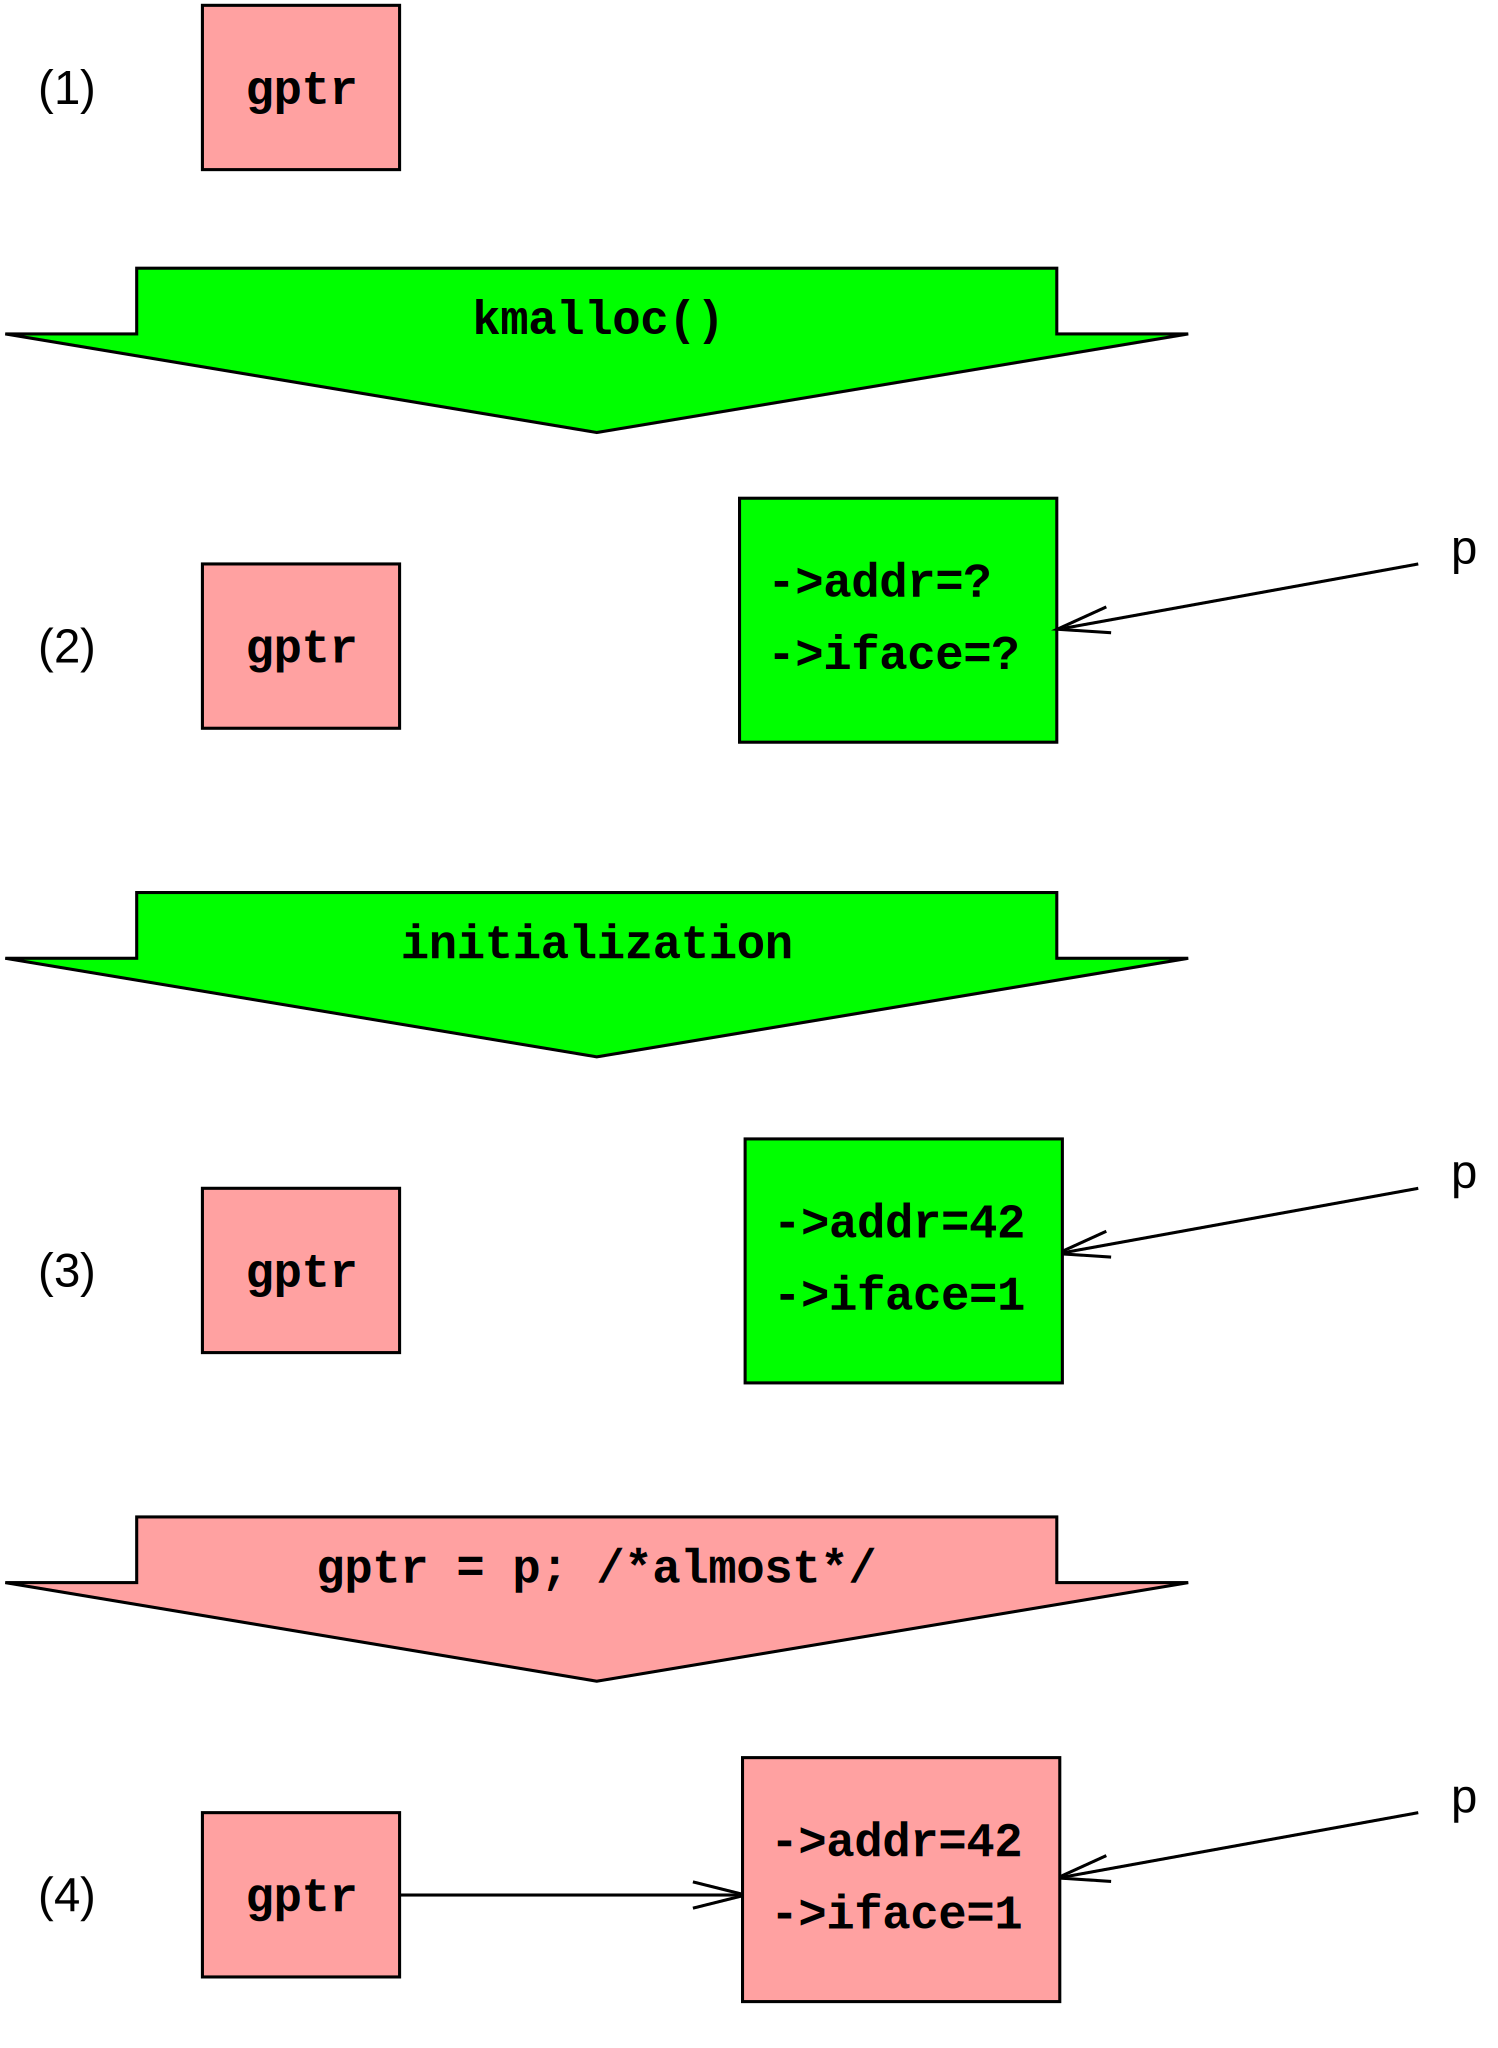
\includegraphics{defer/RCUListInsertClassic}}
\caption{Insertion With Concurrent Readers}
\label{fig:defer:Insertion With Concurrent Readers}
\end{figure}

To minimize implementability concerns, we focus on a minimal
data structure, which consists of a single global pointer that is either
\co{NULL} or references a single structure.
Minimal though it might be, this data structure is heavily used in
production~\cite{GeoffRomer2018C++DeferredReclamationP0561R4}.
A classic approach for insertion is shown in
Figure~\ref{fig:defer:Insertion With Concurrent Readers},
which shows four states with time advancing from top to bottom.
The first row shows the initial state, with \co{gptr} equal to \co{NULL}.
In the second row, we have allocated a structure which is uninitialized,
as indicated by the question marks.
In the third row, we have initialized the structure.
Finally, in the fourth and final row, we have updated \co{gptr} to
reference the newly allocated and initialized element.

We might hope that this assignment to \co{gptr} could use a simple
C-language assignment statement.
Unfortunately,
Section~\ref{sec:toolsoftrade:Shared-Variable Shenanigans}
dashes these hopes.
Therefore, the updater cannot use a simple C-language assignment, but
must instead use \co{smp_store_release()} as shown in the figure,
or, as will be seen, \co{rcu_assign_pointer()}.

Similarly, one might hope that readers could use a single C-language
assignment to fetch the value of \co{gptr}, and be guaranteed to either
get the old value of \co{NULL} or to get the newly installed pointer,
but either way see a valid result.
Unfortunately, Section~\ref{sec:toolsoftrade:Shared-Variable Shenanigans}
dashes these hopes as well.
To obtain this guarantee, readers must instead use \co{READ_ONCE()},
or, as will be seen, \co{rcu_dereference()}.
However, on most modern computer systems, each of these read-side primitives
can be implemented with a single load instruction, exactly the instruction
that would normally be used in single-threaded code.

Reviewing \cref{fig:defer:Insertion With Concurrent Readers}
from the viewpoint of readers, in the first three states all readers
see \co{gptr} having the value \co{NULL}.
Upon entering the fourth state, some readers might see \co{gptr} still
having the value \co{NULL} while others might see it referencing the
newly inserted element, but after some time, all readers will see this
new element.
At all times, all readers will see \co{gptr} as containing a valid pointer.
Therefore, it really is possible to add new data to linked data structures
while allowing concurrent readers to execute the same sequence of machine
instructions that is normally used in single-threaded code.
This no-cost approach to concurrent reading provides excellent performance
and scalability, and also is eminently suitable for real-time use.

\begin{figure}[tb]
\centering
\resizebox{3in}{!}{\includegraphics{defer/RCUListDeleteClassic}}
\caption{Deletion With Concurrent Readers}
\label{fig:defer:Deletion With Concurrent Readers}
\end{figure}

Insertion is of course quite useful, but sooner or later, it will also
be necessary to delete data.
As can be seen in
Figure~\ref{fig:defer:Deletion With Concurrent Readers},
the first step is easy.
Again taking the lessons from
Section~\ref{sec:toolsoftrade:Shared-Variable Shenanigans}
to heart, \co{smp_store_release()} is used to \co{NULL} the pointer,
thus moving from the first row to the second in the figure.
At this point, pre-existing readers see the old structure with
\co{->addr} of 42 and \co{->iface} of 1, but new readers will see
a \co{NULL} pointer, that is, concurrent readers can disagree on
the state, as indicated by the ``2 Versions'' in the figure.

\QuickQuizSeries{%
\QuickQuizB{
	Why does
	Figure~\ref{fig:defer:Deletion With Concurrent Readers}
	use \co{smp_store_release()} given that it is storing
	a \co{NULL} pointer?
	Wouldn't \co{WRITE_ONCE()} work just as well in this case,
	given that there is no structure initialization to order
	against the store of the \co{NULL} pointer?
}\QuickQuizAnswerB{
	Yes, it would.

	Because a \co{NULL} pointer is being assigned, there is nothing
	to order against, so there is no need for \co{smp_store_release()}.
	In contrast, when assigning a non-\co{NULL} pointer, it is
	necessary to use \co{smp_store_release()} in order to ensure
	that initialization of the pointed-to structure is carried
	out before assignment of the pointer.

	In short, \co{WRITE_ONCE()} would work, and would
	save a little bit of CPU time on some architectures.
	However, as we will see, software-engineering concerns
	will motivate use of a special \co{rcu_assign_pointer()}
	that is quite similar to \co{smp_store_release()}.
}\QuickQuizEndB
%
\QuickQuizE{
	Readers running concurrently each other and with the procedure
	outlined in
	Figure~\ref{fig:defer:Deletion With Concurrent Readers}
	can disagree on the value of \co{gptr}.
	Isn't that just a wee bit problematic???
}\QuickQuizAnswerE{
	Not necessarily.

	As hinted at in Sections~\ref{sec:cpu:Hardware Optimizations}
	and~\ref{sec:cpu:Hardware Free Lunch?},
	speed-of-light delays mean that a computer's data is always
	stale compared to whatever external reality that data is intended
	to model.

	Real-world algorithms therefore absolutely must tolerate
	inconsistancies between external reality and the in-computer
	data reflecting that reality.
	Many of those algorithms are also able to tolerate some degree
	of inconsistency within the in-computer data.
	Section~\ref{sec:datastruct:RCU-Protected Hash Table Discussion}
	discusses this point in more detail.

	Please note that this need to tolerate inconsistent and stale
	data is not limited to RCU\@.
	It also applies to reference counting, hazard pointers, sequence
	locks, and even to some locking use cases.
	For example, if you compute some quantity while holding a lock,
	but use that quantity after releasing that lock,
	you might well be using stale data.
	After all, the data that quantity is based on might change
	arbitrarily as soon as the lock is released.

	So yes, RCU readers can see stale and inconsistent data, but no,
	this is not necessarily problematic.
	And, when needed, there are RCU usage patterns that avoid both
	staleness and inconsistency~\cite{Arcangeli03}.
}\QuickQuizEndE
}

We get back to a single version simply by waiting for all the
pre-existing readers to complete, as shown in row~3.
At that point, all the pre-existing readers are done, and no later
reader has a path to the old data item, so there can no longer be
any readers referencing it.
It may therefore be safely freed, as shown on row~4.

Thus, given a way to wait for pre-existing readers to complete,
it is possible to both add data to and remove data from a linked
data structure, despite the readers executing the same sequence
of machine instructions that would be appropriate for single-threaded
execution.
So perhaps going all the way was not too far after all!

But how can we tell when all of the pre-existing readers have in
fact completed?
This question is the topic of the next section.

\subsubsection{Waiting for Readers}
\label{sec:defer:Waiting for Readers}

It is tempting to base reader waiting on reference counting, but
Figure~\ref{fig:count:Atomic Increment Scalability on x86}
in
Chapter~\ref{chp:Counting}
shows that concurrent reference counting results in extreme overhead,
as we already saw in
Section~\ref{sec:defer:Reference Counting}.
Hazard pointers profoundly reduce this overhead, but, as we saw in
Section~\ref{sec:defer:Hazard Pointers}, not to zero.
Nevertheless, many RCU implementations make very careful cache-local
use of counters.

A second approach observes that memory synchronization is expensive,
and therefore uses registers instead, namely each CPU's or thread's
program counter (PC), thus imposing no overhead on readers, at least
in the absence of concurrent updates.
The updater polls each relevant PC, and if that PC is not within read-side
code, then the corresponding CPU or thread is within a quiescent state,
in turn signaling the completion of any reader that might have access
to the newly removed data element.
Once all CPU's or thread's PCs have been observed to be outside of any
reader, the grace period has completed.
Please note that this approach poses some serious challenges, including
memory ordering, functions that are \emph{sometimes} invoked from readers,
and ever-exciting code-motion optimizations.
Nevertheless, this approach is said to be used in
production~\cite{MikeAsh2015Apple}.

A third approach is to simply wait for a fixed period of time that is
long enough to comfortably exceed the lifetime of any reasonable
reader~\cite{Jacobson93,AjuJohn95}.
This can work quite well in hard real-time systems~\cite{YuxinRen2018RTRCU},
but in less exotic
settings, Murphy says that it is critically important to be prepared
even for unreasonably long-lived readers.
To see this, consider the consequences of failing do so:
A data item will be freed while the unreasonable reader is still
referencing it, and that item might well be immediately reallocated,
possibly even as a data item of some other type.
The unreasonable reader and the unwitting reallocator would then
be attempting to use the same memory for two very different purposes.
The ensuing mess will at best be exceedingly difficult to debug.

A fourth approach is to wait forever, secure in the knowledge that
doing so will accommodate even the most unreasonable reader.
This approach is also called ``leaking memory'', and has a bad reputation
due to the fact that memory leaks often require untimely and
inconvenient reboots.
Nevertheless, this is a viable strategy when the update rate and the
uptime are both sharply bounded.
For example, this approach could work well in a high-availability
cluster where systems were periodically crashed in order to ensure
that cluster really remained highly available.\footnote{
	The program that forces the periodic crashing is sometimes
	known as a ``chaos monkey'':
	\url{https://netflix.github.io/chaosmonkey/}.
	However, it might also be a mistake to neglect chaos caused
	by systems running for too long.}
Leaking the memory is also a viable strategy in environments having
garbage collectors, in which case the garbage collector can be thought
of as plugging the leak~\cite{Kung80}.
However, if your environment lacks a garbage collector, read on!

A fifth approach avoids the period crashes in favor of periodically
``stopping the world'', as exemplified by the traditional stop-the-world
garbage collector.
This approach was also heavily used during the decades before
ubiquitous connectivity, when it was common practice to power systems
off at the end of each working day.
However, in today's always-connected always-on world, stopping the world
can gravely degrade response times, which has been one motivation for the
development of concurrent garbage collectors~\cite{DavidFBacon2003RTGC}.
Furthermore, although we need all pre-existing readers to complete, we do
not need them all to complete at the same time.

This observation leads to the sixth approach, which is stopping
one CPU or thread at a time.
This approach has the advantage of not degrading reader response times
at all, let alone gravely.
Furthermore, numerous applications already have states (termed
\emph{quiescent states}) that can be
reached only after all pre-existing readers are done.
In transaction-processing systems, the time between a pair of
successive transactions might be a quiescent state.
In reactive systems, the state between a pair of successive events
might be a quiescent state.
Within non-preemptive operating-systems kernels, a context switch can be
a quiescent state~\cite{McKenney98}.
Either way, once all CPUs and/or threads have passed through a quiescent
state, the system is said to have completed a \emph{grace period},
at which point all readers in existence at the start of that grace period
are guaranteed to have completed.
As a result, it is also guaranteed to be safe to free any removed data
items that were removed prior to the start of that grace period.\footnote{
	It is possible to do much more with RCU than simply defer
	reclamation of memory, but deferred reclamation is RCU's most
	common use case, and is therefore an excellent place to start.}

Within a non-preemptive operating-system kernel, for context switch to be
a valid quiescent state, readers must be prohibited from blocking while
referencing a given instance data structure obtained via the \co{gptr}
pointer shown in
Figures~\ref{fig:defer:Insertion With Concurrent Readers}
and~\ref{fig:defer:Deletion With Concurrent Readers}.
This no-blocking constraint is consistent with similar constraints
on pure spinlocks, where a CPU is forbidden from blocking while
holding a spinlock.
Without this constraint, all CPUs might be consumed by threads
spinning attempting to acquire a spinlock held by a blocked thread.
The spinning threads will not relinquish their CPUs until they acquire
the lock, but the thread holding the lock cannot possibly release it
until one of the spinning threads relinquishes a CPU\@.
This is a classic deadlock situation, and this deadlock is avoided
by forbidding blocking while holding a spinlock.

Again, this same constraint is imposed on reader threads dereferencing
\co{gptr}: such threads are not allowed to block until after
they are done using the pointed-to data item.
Returning to the second row of
Figure~\ref{fig:defer:Deletion With Concurrent Readers},
where the updater has just completed executing the \co{smp_store_release()},
imagine that CPU~0 executes a context switch.
Because readers are not permitted to block while traversing the linked
list, we are guaranteed that all prior readers that might have been running on
CPU~0 will have completed.
Extending this line of reasoning to the other CPUs, once each CPU has
been observed executing a context switch, we are guaranteed that all
prior readers have completed, and that there are no longer any reader
threads referencing the newly removed data element.
The updater can then safely free that data element, resulting in the
state shown at the bottom of
Figure~\ref{fig:defer:Deletion With Concurrent Readers}.

\begin{figure}[tb]
\centering
\resizebox{3in}{!}{\includegraphics{defer/QSBRGracePeriod}}
\caption{QSBR: Waiting for Pre-Existing Readers}
\label{fig:defer:QSBR: Waiting for Pre-Existing Readers}
\end{figure}

This approach is termed \emph{quiescent state based reclamation}
(QSBR)~\cite{ThomasEHart2006a}.
A QSBR schematic is shown in
Figure~\ref{fig:defer:QSBR: Waiting for Pre-Existing Readers},
with time advancing from the top of the figure to the bottom.
CPU~1 does the \co{WRITE_ONCE()} that removes the current data
item (presumably having previously read the pointer value and
availed itself of appropriate synchronization), then waits
for readers.
This wait operation results in an immediate context switch, which is a
quiescent state (denoted by the pink circle), which in turn means that
all prior reads on CPU~1 have completed.
Next, CPU~2 does a context switch, so that all readers on CPUs~1 and~2
are now known to have completed.
Finally, CPU~3 does a context switch.
At this point, all readers throughout the entire system are known to
have completed, so the grace period ends, permitting CPU~1 to free
the old data item.

\QuickQuiz{
	In Figure~\ref{fig:defer:QSBR: Waiting for Pre-Existing Readers},
	the last of CPU~3's readers that could possibly have
	access to the old data item ended before the grace period
	even started!
	So why would anyone bother waiting until CPU~3's later context
	switch???
}\QuickQuizAnswer{
	Because that waiting is exactly what enables readers to use
	the same sequence of instructions that is appropriate for
	single-theaded situations.
	In other words, this additional ``redundant'' waiting enables
	excellent read-side performance, scalability, and real-time
	response.
}\QuickQuizEnd

\subsubsection{Toy Implementation}
\label{sec:defer:Toy Implementation}

Although production-quality QSBR implementations can be quite complex,
a toy non-preemptive Linux-kernel implementation is exceedingly simple:

\begin{VerbatimN}[samepage=true]
void synchronize_rcu(void)
{
	int cpu;

	for_each_online_cpu(cpu)
		sched_setaffinity(current->pid, cpumask_of(cpu));
}
\end{VerbatimN}

The \co{for_each_online_cpu()} primitive iterates over all CPUs, and
the \co{sched_setaffinity()} function causes the current thread to
execute on the specified CPU, which forces the destination CPU to execute
a context switch.
Therefore, once the \co{for_each_online_cpu()} has completed, each CPU
has executed a context switch, which in turn guarantees that
all pre-existing reader threads have completed.

\begin{listing}[tbp]
\begin{fcvlabel}[ln:defer:Insertion and Deletion With Concurrent Readers]
\begin{VerbatimL}[commandchars=\\\[\]]
struct route *gptr;

int access_route(int (*f)(struct route *rp))
{
	int ret = -1;
	struct route *rp;

	rcu_read_lock();
	rp = rcu_dereference(gptr);
	if (rp)
		ret = f(rp);		\lnlbl[access_rp]
	rcu_read_unlock();
	return ret;
}

struct route *ins_route(struct route *rp)
{
	struct route *old_rp;

	spin_lock(&route_lock);
	old_rp = gptr;
	rcu_assign_pointer(gptr, rp);
	spin_unlock(&route_lock);
	return old_rp;
}

int del_route(void)
{
	struct route *old_rp;

	spin_lock(&route_lock);
	old_rp = gptr;
	RCU_INIT_POINTER(gptr, NULL);
	spin_unlock(&route_lock);
	synchronize_rcu();
	free(old_rp);
	return !!old_rp;
}
\end{VerbatimL}
\end{fcvlabel}
\caption{Insertion and Deletion With Concurrent Readers}
\label{lst:defer:Insertion and Deletion With Concurrent Readers}
\end{listing}

Please note that this approach is \emph{not} production quality.
Correct handling of a number of corner cases and the need for a number
of powerful optimizations mean that production-quality implementations
are quite complex.
In addition, RCU implementations for preemptible environments
require that readers actually do something, which in non-real-time
Linux-kernel environments can be as simple as defining
\co{rcu_read_lock()} and \co{rcu_read_unlock()} as \co{preempt_disable()}
and \co{preempt_enable()}, respectively.\footnote{
	Some toy RCU implementations that handle preempted
	read-side critical sections are shown in
	Appendix~\ref{chp:app:``Toy'' RCU Implementations}.}
However, this simple non-preemptible approach is conceptually complete,
and demonstrates that it really is possible to provide read-side
synchronization at zero cost, even in the face of concurrent updates.
In fact,
Listing~\ref{lst:defer:Insertion and Deletion With Concurrent Readers}
shows how reading (\co{access_route()}),
Figure~\ref{fig:defer:Insertion With Concurrent Readers}'s
insertion (\co{ins_route()}) and
Figure~\ref{fig:defer:Deletion With Concurrent Readers}'s
deletion (\co{del_route()}) can
be implemented.
(A slightly more capable routing table is shown in
Section~\ref{sec:defer:RCU for Pre-BSD Routing}.)

\QuickQuizSeries{%
\QuickQuizB{
	What is the point of \co{rcu_read_lock()} and \co{rcu_read_unlock()} in
	Listing~\ref{lst:defer:Insertion and Deletion With Concurrent Readers}?
	Why not just let the quiescent states speak for themselves?
}\QuickQuizAnswerB{
	Recall that readers are not permitted to pass through a quiescent
	state.
	For example, within the Linux kernel, RCU readers are not permitted
	to execute a context switch.
	Use of \co{rcu_read_lock()} and \co{rcu_read_unlock()} enables
	debug checks for improperly placed quiescent states, making it
	easy to find bugs that would otherwise be difficult to find,
	intermittent, and quite destructive.
}\QuickQuizEndB
%
\QuickQuizE{
	What is the point of \co{rcu_dereference()}, \co{rcu_assign_pointer()}
	and \co{RCU_INIT_POINTER()} in
	Listing~\ref{lst:defer:Insertion and Deletion With Concurrent Readers}?
	Why not just use \co{READ_ONCE()}, \co{smp_store_release()}, and
	\co{WRITE_ONCE()}, respectively?
}\QuickQuizAnswerE{
	The RCU-specific APIs do have similar semantics to the suggested
	replacements, but also enable static-analysis debugging checks
	that complain if an RCU-specific API is invoked on a non-RCU
	pointer and vice versa.
}\QuickQuizEndE
}

Referring back to
Listing~\ref{lst:defer:Insertion and Deletion With Concurrent Readers},
note that \co{route_lock} is used to synchronize between concurrent updaters
invoking \co{ins_route()} and \co{del_route()}.
However, this lock is not acquired by readers invoking \co{access_route()}:
Readers are instead protected by the QSBR techniques described in this section.

Note that \co{ins_route()} simply returns the old value of \co{gptr}, which
Figure~\ref{fig:defer:Insertion With Concurrent Readers} assumed would
always be \co{NULL}.
This means that it is the caller's responsibility to figure out what to
do with a non-\co{NULL} value, a task complicated by the fact that
readers might still be referencing it for an indeterminate period of time.
Callers might use one of the following approaches:

\begin{enumerate}
\item	Use \co{synchronize_rcu()} to safely free the pointed-to structure.
	Although this approach is correct from an RCU perspective, it
	arguably has software-engineering leaky-API problems.
\item	Trip an assertion if the returned pointer is non-\co{NULL}.
\item	Pass the returned pointer to a later invocation of
	\co{ins_route()} to restore the earlier value.
\end{enumerate}

In contrast, \co{del_route()} uses \co{synchronize_rcu()} and
\co{free()} to safely free the newly deleted data item.

\QuickQuiz{
	But what if the old structure needs to be freed, but the caller
	of \co{ins_route()} cannot block, perhaps due to performance
	considerations or perhaps because the caller is executing within
	an RCU read-side critical section?
}\QuickQuizAnswer{
	A \co{call_rcu()} function, which is described in
	Section~\ref{sec:defer:Wait For Pre-Existing RCU Readers},
	permits asynchronous grace-period waits.
}\QuickQuizEnd

This example shows one general approach to reading and updating
RCU-protected data structures, however, there is quite a variety
of use cases, several of which are covered in
Section~\ref{sec:defer:RCU Usage}.

In summary, it is in fact possible to create concurrent linked data
structures that can be traversed by readers executing the same sequence
of machine instructions that would be executed by single-threaded readers.
The next section summarizes RCU's high-level properties.

\subsubsection{RCU Properties}
\label{sec:defer:RCU Properties}

A key RCU property is that reads need not wait for updates.
This property enables RCU implementations to provide low-cost or even
no-cost readers, resulting in low overhead and excellent scalability.
This property also allows RCU readers and updaters to make useful
concurrent forward progress.
In contrast, conventional synchronization primitives must enforce strict
mutual exclusion using expensive instructions, thus increasing overhead
and degrading scalability, but also typically prohibiting readers and
updaters from making useful concurrent forward progress.

\QuickQuiz{
	Doesn't Section~\ref{sec:defer:Sequence Locks}'s seqlock
	also permit readers and updaters to make useful concurrent
	forward progress?
}\QuickQuizAnswer{
	Yes and no.
	Although seqlock readers can run concurrently with
	seqlock writers, whenever this happens, the \co{read_seqretry()}
	primitive will force the reader to retry.
	This means that any work done by a seqlock reader running concurrently
	with a seqlock updater will be discarded and the redone upon retry.
	So seqlock readers can \emph{run} concurrently with updaters,
	but they cannot actually get any work done in this case.

	In contrast, RCU readers can perform useful work even in presence
	of concurrent RCU updaters.

	However, both reference counters
	(Section~\ref{sec:defer:Reference Counting})
	and hazard pointers
	(Section~\ref{sec:defer:Hazard Pointers})
	really do permit useful concurrent forward progress for both
	updaters and readers, just at somewhat greater cost.
	Please see
	Section~\ref{sec:defer:Which to Choose?}
	for a comparison of these different solutions to the
	deferred-reclamation problem.
}\QuickQuizEnd

RCU delimits readers with \co{rcu_read_lock()} and \co{rcu_read_unlock()},
and ensures that each reader has a coherent view of each object
(see \cref{fig:defer:Deletion With Concurrent Readers}) by
maintaining multiple versions of objects and using update-side primitives
such as \co{synchronize_rcu()} to ensure that objects are not
freed until after the completion of all readers that might be using them.
RCU uses \co{rcu_assign_pointer()} and \co{rcu_dereference()} to provide
efficient and scalable mechanisms for publishing and reading new versions
of an object, respectively.
These mechanisms distribute the work among read and
update paths in such a way as to make read paths extremely fast, using
replication and weakening optimizations in a manner similar to
hazard pointers, but without the need for read-side retries.
In some cases, including \co{CONFIG_PREEMPT=n} Linux kernels,
RCU's read-side primitives have zero overhead.

But are these properties actually useful in practice?
This question is taken up by the next section.

\subsubsection{Practical Applicability}
\label{sec:defer:Practical Applicability}

\begin{figure}[tb]
\centering
\resizebox{3in}{!}{\includegraphics{defer/linux-RCU}}
\caption{RCU Usage in the Linux Kernel}
\label{fig:defer:RCU Usage in the Linux Kernel}
\end{figure}

RCU has been used in the Linux kernel since
October 2002~\cite{Torvalds2.5.43}.
Use of the RCU API has increased substantially since that time,
as can be seen in
Figure~\ref{fig:defer:RCU Usage in the Linux Kernel}.
In fact, code very similar to that in
Listing~\ref{lst:defer:Insertion and Deletion With Concurrent Readers}
is used in the Linux kernel.
RCU has enjoyed heavy use both prior to and since its acceptance
in the Linux kernel, as discussed in
\cref{sec:defer:RCU Related Work}.

It is therefore safe to say that RCU enjoys wide practical applicability.

The minimal example discussed in this section is a good introduction to RCU\@.
However, effective use of RCU often requires that you think differently
about your problem.
It is therefore useful to examine RCU's fundamentals, a task taken up
by the following section.

% defer/rcufundamental.tex

\subsection{RCU Fundamentals}
\label{sec:defer:RCU Fundamentals}
\OriginallyPublished{Section}{sec:defer:RCU Fundamentals}{RCU Fundamentals}{Linux Weekly News}{PaulEMcKenney2007WhatIsRCUFundamentally}

RCU is made up of three fundamental mechanisms, the first being
used for insertion, the second being used for deletion, and the third
being used to allow readers to tolerate concurrent insertions and deletions.
Section~\ref{sec:defer:Publish-Subscribe Mechanism}
describes the publish-subscribe mechanism used for insertion,
Section~\ref{sec:defer:Wait For Pre-Existing RCU Readers}
describes how waiting for pre-existing RCU readers enabled deletion,
and
Section~\ref{sec:defer:Maintain Multiple Versions of Recently Updated Objects}
discusses how maintaining multiple versions of recently updated objects
permits concurrent insertions and deletions.
Finally,
Section~\ref{sec:defer:Summary of RCU Fundamentals}
summarizes RCU fundamentals.

\subsubsection{Publish-Subscribe Mechanism}
\label{sec:defer:Publish-Subscribe Mechanism}

% @@@ Slim down presentation, refer to toolsoftrade and memorder.
% @@@ Summarize care and feeding of address dependencies.
% @@@ Mention language/compiler support being a work in progress.

\begin{listing}[tbp]
\begin{VerbatimL}
struct foo {
	int a;
	int b;
	int c;
};
struct foo *gp = NULL;

/* . . . */

p = kmalloc(sizeof(*p), GFP_KERNEL);
p->a = 1;
p->b = 2;
p->c = 3;
gp = p;
\end{VerbatimL}
\caption{Data Structure Publication (Unsafe)}
\label{lst:defer:Data Structure Publication (Unsafe)}
\end{listing}

One key attribute of RCU is the ability to safely scan data, even
though that data is being modified concurrently.
To provide this ability for concurrent insertion,
RCU uses what can be thought of as a publish-subscribe mechanism.
For example, consider an initially \co{NULL} global pointer
\co{gp} that is to be modified to point to a newly allocated
and initialized data structure.
The code fragment shown in
Listing~\ref{lst:defer:Data Structure Publication (Unsafe)}
(with the addition of appropriate locking)
might be used for this purpose.

Unfortunately, there is nothing forcing the compiler and CPU to execute
the last four assignment statements in order.
If the assignment to \co{gp} happens before the initialization
of \co{p} fields, then concurrent readers could see the
uninitialized values.
Memory barriers are required to keep things ordered, but memory barriers
are notoriously difficult to use.
We therefore encapsulate them into a primitive
\co{rcu_assign_pointer()} that has publication semantics.
The last four lines would then be as follows:

\begin{VerbatimN}[samepage=true]
p->a = 1;
p->b = 2;
p->c = 3;
rcu_assign_pointer(gp, p);
\end{VerbatimN}

The \co{rcu_assign_pointer()}
would \emph{publish} the new structure, forcing both the compiler
and the CPU to execute the assignment to \co{gp} \emph{after}
the assignments to the fields referenced by \co{p}.

However, it is not sufficient to only enforce ordering at the
updater, as the reader must enforce proper ordering as well.
Consider for example the following code fragment:

\begin{VerbatimN}[samepage=true]
p = gp;
if (p != NULL) {
	do_something_with(p->a, p->b, p->c);
}
\end{VerbatimN}

Although this code fragment might well seem immune to misordering,
unfortunately, the
DEC Alpha CPU~\cite{PaulMcKenney2005i,PaulMcKenney2005j}
and value-speculation compiler optimizations can, believe it or not,
cause the values of \co{p->a}, \co{p->b}, and
\co{p->c} to be fetched before the value of \co{p}.
This is perhaps easiest to see in the case of value-speculation
compiler optimizations, where the compiler guesses the value
of \co{p}, fetches \co{p->a}, \co{p->b}, and
\co{p->c}, and then fetches the actual value of \co{p}
in order to check whether its guess was correct.
This sort of optimization is quite aggressive, perhaps insanely so,
but does actually occur in the context of profile-driven optimization.

Clearly, we need to prevent this sort of skullduggery on the
part of both the compiler and the CPU.
The \co{rcu_dereference()} primitive uses
whatever memory-barrier instructions and compiler
directives are required for this purpose:\footnote{
	In the Linux kernel, \co{rcu_dereference()} is implemented via
	a volatile cast, and, on DEC Alpha, a memory barrier instruction.
	In the C11 and C++11 standards, \co{memory_order_consume}
	is intended to provide longer-term support for \co{rcu_dereference()},
	but no compilers implement this natively yet.
	(They instead strengthen \co{memory_order_consume} to
	\co{memory_order_acquire}, thus emitting a needless memory-barrier
	instruction on weakly ordered systems.)}

\begin{VerbatimN}[samepage=true]
rcu_read_lock();
p = rcu_dereference(gp);
if (p != NULL) {
	do_something_with(p->a, p->b, p->c);
}
rcu_read_unlock();
\end{VerbatimN}

The \co{rcu_dereference()} primitive can thus be thought of
as \emph{subscribing} to a given value of the specified pointer,
guaranteeing that subsequent dereference operations will see any
initialization that occurred before the corresponding
\co{rcu_assign_pointer()} operation that published that pointer.
The \co{rcu_read_lock()} and \co{rcu_read_unlock()}
calls are absolutely required: they define the extent of the
RCU read-side critical section.
Their purpose is explained in
Section~\ref{sec:defer:Wait For Pre-Existing RCU Readers},
however, they never spin or block, nor do they prevent the
\co{list_add_rcu()} from executing concurrently.
In fact, in non-\co{CONFIG_PREEMPT} kernels, they generate
absolutely no code.

\begin{figure}[tb]
\centering
\resizebox{3in}{!}{\includegraphics{defer/Linux_list}}
\caption{Linux Circular Linked List}
\label{fig:defer:Linux Circular Linked List}
\end{figure}

\begin{figure}[tb]
\centering
\resizebox{1.8in}{!}{\includegraphics{defer/Linux_list_abbr}}
\caption{Linux Linked List Abbreviated}
\label{fig:defer:Linux Linked List Abbreviated}
\end{figure}

Although \co{rcu_assign_pointer()} and
\co{rcu_dereference()} can in theory be used to construct any
conceivable RCU-protected data structure, in practice it is often better
to use higher-level constructs.
Therefore, the \co{rcu_assign_pointer()} and
\co{rcu_dereference()}
primitives have been embedded in special RCU variants of Linux's
list-manipulation API.
Linux has two variants of doubly linked list, the circular
\co{struct list_head} and the linear
\co{struct hlist_head}/\co{struct hlist_node} pair.
The former is laid out as shown in
Figure~\ref{fig:defer:Linux Circular Linked List},
where the green (leftmost) boxes represent the list header and the blue
(rightmost three) boxes represent the elements in the list.
This notation is cumbersome, and will therefore be abbreviated as shown in
Figure~\ref{fig:defer:Linux Linked List Abbreviated},
which shows only the non-header (blue) elements.

\begin{listing}[tbp]
\begin{linelabel}[ln:defer:RCU Data Structure Publication]
\begin{VerbatimL}[commandchars=\\\[\]]
struct foo {
	struct list_head *list;
	int a;
	int b;
	int c;
};
LIST_HEAD(head);

/* . . . */

p = kmalloc(sizeof(*p), GFP_KERNEL);
p->a = 1;
p->b = 2;
p->c = 3;
list_add_rcu(&p->list, &head);		\lnlbl[add_rcu]
\end{VerbatimL}
\end{linelabel}
\caption{RCU Data Structure Publication}
\label{lst:defer:RCU Data Structure Publication}
\end{listing}

Adapting the pointer-publish example for the linked list results in
the code shown in
Listing~\ref{lst:defer:RCU Data Structure Publication}.

Line~\ref{ln:defer:RCU Data Structure Publication:add_rcu}
must be protected by some synchronization mechanism (most
commonly some sort of lock) to prevent multiple \co{list_add_rcu()}
instances from executing concurrently.
However, such synchronization does not prevent this \co{list_add()}
instance from executing concurrently with RCU readers.

Subscribing to an RCU-protected list is straightforward:

\begin{VerbatimN}[samepage=true]
rcu_read_lock();
list_for_each_entry_rcu(p, head, list) {
	do_something_with(p->a, p->b, p->c);
}
rcu_read_unlock();
\end{VerbatimN}

The \co{list_add_rcu()} primitive publishes an entry, inserting it at
the head of the specified list, guaranteeing that the corresponding
\co{list_for_each_entry_rcu()} invocation will properly subscribe to
this same entry.

\QuickQuiz{}
	What prevents the \co{list_for_each_entry_rcu()} from
	getting a segfault if it happens to execute at exactly the same
	time as the \co{list_add_rcu()}?
\QuickQuizAnswer{
	On all systems running Linux, loads from and stores
	to pointers are atomic, that is, if a store to a pointer occurs at
	the same time as a load from that same pointer, the load will return
	either the initial value or the value stored, never some bitwise
	mashup of the two.
	In addition, the \co{list_for_each_entry_rcu()} always proceeds
	forward through the list, never looking back.
	Therefore, the \co{list_for_each_entry_rcu()} will either see
	the element being added by \co{list_add_rcu()} or it will not,
	but either way, it will see a valid well-formed list.
} \QuickQuizEnd

\begin{figure}[tb]
\centering
\resizebox{3in}{!}{\includegraphics{defer/Linux_hlist}}
\caption{Linux Linear Linked List}
\label{fig:defer:Linux Linear Linked List}
\end{figure}

Linux's other doubly linked list, the hlist,
is a linear list, which means that
it needs only one pointer for the header rather than the two
required for the circular list, as shown in
Figure~\ref{fig:defer:Linux Linear Linked List}.
Thus, use of hlist can halve the memory consumption for the hash-bucket
arrays of large hash tables.
As before, this notation is cumbersome, so hlists will be abbreviated
in the same way lists are, as shown in
Figure~\ref{fig:defer:Linux Linked List Abbreviated}.

\begin{listing}[tbp]
\begin{linelabel}[ln:defer:RCU hlist Publication]
\begin{VerbatimL}[commandchars=\\\[\]]
struct foo {
	struct hlist_node *list;
	int a;
	int b;
	int c;
};
HLIST_HEAD(head);

/* . . . */

p = kmalloc(sizeof(*p), GFP_KERNEL);
p->a = 1;
p->b = 2;
p->c = 3;
hlist_add_head_rcu(&p->list, &head);	\lnlbl[add_head]
\end{VerbatimL}
\end{linelabel}
\caption{RCU {\tt hlist} Publication}
\label{lst:defer:RCU hlist Publication}
\end{listing}

Publishing a new element to an RCU-protected hlist is quite similar
to doing so for the circular list,
as shown in Listing~\ref{lst:defer:RCU hlist Publication}.

As before, line~\ref{ln:defer:RCU hlist Publication:add_head}
must be protected by some sort of synchronization
mechanism, for example, a lock.

Subscribing to an RCU-protected hlist is also similar to the
circular list:

\begin{VerbatimN}[samepage=true]
rcu_read_lock();
hlist_for_each_entry_rcu(p, head, list) {
	do_something_with(p->a, p->b, p->c);
}
rcu_read_unlock();
\end{VerbatimN}

\begin{table*}[tb]
\renewcommand*{\arraystretch}{1.2}
\centering
\footnotesize\OneColumnHSpace{-0.4in}
\begin{tabular}{llll}
\toprule
Category  & Publish	& Retract	& Subscribe \\
\midrule
Pointers  & \tco{rcu_assign_pointer()}
			& \tco{rcu_assign_pointer(..., NULL)}
					& \tco{rcu_dereference()} \\
\midrule
Lists     & \parbox[c][0.37in][c]{1.3in}{
		\co{list_add_rcu()} \\
		\co{list_add_tail_rcu()} \\
		\co{list_replace_rcu()} }
			& \tco{list_del_rcu()}
					& \tco{list_for_each_entry_rcu()} \\
\midrule
Hlists    & \parbox[c][0.5in][c]{1.3in}{
		\co{hlist_add_behind_rcu()} \\
		\co{hlist_add_before_rcu()} \\
		\co{hlist_add_head_rcu()} \\
		\co{hlist_replace_rcu()} }
			& \tco{hlist_del_rcu()}
					& \tco{hlist_for_each_entry_rcu()} \\
\bottomrule
\end{tabular}
\caption{RCU Publish and Subscribe Primitives}
\label{tab:defer:RCU Publish and Subscribe Primitives}
\end{table*}

The set of RCU publish and subscribe primitives are shown in
Table~\ref{tab:defer:RCU Publish and Subscribe Primitives},
along with additional primitives to ``unpublish'', or retract.

Note that the \co{list_replace_rcu()}, \co{list_del_rcu()},
\co{hlist_replace_rcu()}, and \co{hlist_del_rcu()}
APIs add a complication.
When is it safe to free up the data element that was replaced or
removed?
In particular, how can we possibly know when all the readers
have released their references to that data element?

These questions are addressed in the following section.

\subsubsection{Wait For Pre-Existing RCU Readers}
\label{sec:defer:Wait For Pre-Existing RCU Readers}

In its most basic form, RCU is a way of waiting for things to finish.
Of course, there are a great many other ways of waiting for things to
finish, including reference counts, reader-writer locks, events, and so on.
The great advantage of RCU is that it can wait for each of
(say) 20,000 different things without having to explicitly
track each and every one of them, and without having to worry about
the performance degradation, scalability limitations, complex deadlock
scenarios, and memory-leak hazards that are inherent in schemes
using explicit tracking.

In RCU's case, each of the things waited on is called an
\emph{RCU read-side critical section}.
As hinted at in
Section~\ref{sec:defer:Toy Implementation}, an RCU read-side critical
section starts with an \co{rcu_read_lock()} primitive, and ends with a
corresponding \co{rcu_read_unlock()} primitive.
RCU read-side critical sections can be nested, and may contain pretty
much any code, as long as that code does not contain a quiescent state,
for example, within the Linux kernel, it is illegal to sleep within
an RCU read-side critical section because a context switch is a quiescent
state.\footnote{
	However, a special form of RCU called SRCU~\cite{PaulEMcKenney2006c}
	does permit general sleeping in SRCU read-side critical sections.}
If you abide by these conventions, you can use RCU to wait for \emph{any}
pre-existing RCU read-side critical section to complete, and
\co{synchronize_rcu()} does the actual waiting.

% @@@ citations? @@@ RCU accomplishes this feat by indirectly determining
% when these other things have finished~\cite{PaulEMcKenney2007whatisRCU,
% PaulEMcKenney2007PreemptibleRCU}.

\begin{figure}[tb]
\centering
\resizebox{3in}{!}{\includegraphics{defer/RCUGuaranteeFwd}}
\caption{RCU Reader and Later Grace Period}
\label{fig:defer:RCU Reader and Later Grace Period}
\end{figure}

The relationship between an RCU read-side critical section and a later
RCU grace period is an if-then relationship, as illustrated by
Figure~\ref{fig:defer:RCU Reader and Later Grace Period}.
If any portion of a given critical section precedes the beginning of
a given grace period, then RCU guarantees that all of that critical
section will precede the end of that grace period.
In the figure, because \co{P0()}'s access to \co{y} precedes
\co{P1()}'s access to this same variable, it is guaranteed that
\co{P0()}'s access to \co{x} will precede \co{P1()}'s access.
In this case, if \co{y}'s final value is 2, then \co{x}'s
final value is guaranteed to also be 2.

\QuickQuiz{}
	What other final values of \co{x} and \co{y} are possible in
	Figure~\ref{fig:defer:RCU Reader and Later Grace Period}?
\QuickQuizAnswer{
	The \co{x == 2 && y == 2} possibility was called out in the text.
	Given that \co{y == 2} implies \co{x == 2}, we know that
	\co{x == 1 && y == 2} is forbidden.
	The following discussion will show that both
	\co{x == 1 && y == 1} and \co{x == 2 && y == 1} are possible.
} \QuickQuizEnd

\begin{figure}[tb]
\centering
\resizebox{3in}{!}{\includegraphics{defer/RCUGuaranteeRev}}
\caption{RCU Reader and Earlier Grace Period}
\label{fig:defer:RCU Reader and Earlier Grace Period}
\end{figure}

The relationship between an RCU read-side critical section and an earlier
RCU grace period is also an if-then relationship, as illustrated by
Figure~\ref{fig:defer:RCU Reader and Earlier Grace Period}.
If any portion of a given critical section follows the end of
a given grace period, then RCU guarantees that all of that critical
section will follow the beginning of that grace period.
In the figure, because \co{P0()}'s access to \co{x} follows
\co{P1()}'s access to this same variable, it is guaranteed that
\co{P0()}'s access to \co{y} will precede \co{P1()}'s access.
In this case, if \co{x}'s final value is 1, then \co{y}'s
final value is guaranteed to also be 1.

\begin{figure}[tb]
\centering
\resizebox{3in}{!}{\includegraphics{defer/RCUGuaranteeMid}}
\caption{RCU Reader Within Grace Period}
\label{fig:defer:RCU Reader Within Grace Period}
\end{figure}

Finally, as shown in
Figure~\ref{fig:defer:RCU Reader Within Grace Period},
an RCU read-side critical section can be completely overlapped by
an RCU grace period.
In this case, \co{x}'s final value is 1 and \co{y}'s final value is 2.

However, it cannot be the case that \co{x}'s final value is 2 and \co{y}'s
final value is 1.
This would mean that an RCU read-side critical section had completely
overlapped a grace period, which is forbidden.
RCU's wait-for-readers guarantee therefore has two parts:
(1)~If any part of a given RCU read-side critical section precedes
the beginning of a given grace period, then the entirety of that
critical section precedes the end of that grace period.
(2)~If any part of a given RCU read-side critical section follows
the end of a given grace period, then the entirety of that
critical section follows the beginning of that grace period.
This definition is sufficient for almost all RCU-based algorithms, but
for those wanting more,
simple executable formal models of RCU are available
as part of Linux kernel v4.17 and later, as discussed in
Section~\ref{sec:formal:Axiomatic Approaches and RCU}.
In addition, RCU's ordering properties are examined in much
greater detail in Section~\ref{sec:memorder:RCU}.

Although RCU's wait-for-readers capability really is sometimes used to
order the assignment of values to variables as shown in
Figures~\ref{fig:defer:RCU Reader and Later Grace Period}-\ref{fig:defer:RCU Reader Within Grace Period},
it is more frequently used to safely free data elements removed from
a linked structure, as was done in
Section~\ref{sec:defer:Introduction to RCU}.
The general process is illustrated by the following pseudocode:

\begin{enumerate}
\item	Make a change, for example, remove an element from a linked list.
\item	Wait for all pre-existing RCU read-side critical sections to
	completely finish (for example, by using
	\co{synchronize_rcu()}).
\item	Clean up, for example, free the element that was replaced above.
\end{enumerate}

Given that RCU readers can make forward progress while this update
is in progress, different readers might disagree about the state
of the data structure, a topic taken up by the next section.

\subsubsection{Maintain Multiple Versions of Recently Updated Objects}
\label{sec:defer:Maintain Multiple Versions of Recently Updated Objects}

This section demonstrates how RCU maintains multiple versions of
lists to accommodate synchronization-free readers.
Two examples are presented showing how an element
that might be referenced by a given reader must remain intact
while that reader remains in its RCU read-side critical section.
The first example demonstrates deletion of a list element,
and the second example demonstrates replacement of an element.

\paragraph{Example 1: Maintaining Multiple Versions During Deletion}
\label{sec:defer:Example 1: Maintaining Multiple Versions During Deletion}

We can now revisit the deletion example from
Section~\ref{sec:defer:Introduction to RCU},
but now with the benefit of a firm understanding of the fundamental
concepts underlying RCU.
% @@@ \begin{lineref}[ln:defer:Canonical RCU Replacement Example]
% @@@ To begin this new version of the deletion example,
% @@@ we will modify
% @@@ lines~\lnref{search}-\lnref{kfree} in
% @@@ Listing~\ref{lst:defer:Canonical RCU Replacement Example}
% @@@ to read as follows:
% @@@ \end{lineref}

\begin{linelabel}[ln:defer:RCU Deletion From Linked List]
\begin{VerbatimN}[samepage=true,commandchars=\\\[\]]
p = search(head, key);
if (p != NULL) {
	list_del_rcu(&p->list);		\lnlbl[del_rcu]
	synchronize_rcu();		\lnlbl[sync_rcu]
	kfree(p);
}
\end{VerbatimN}
\end{linelabel}

\begin{figure}[tb]
\centering
\resizebox{3in}{!}{\includegraphics{defer/RCUDeletion}}
\caption{RCU Deletion From Linked List}
\label{fig:defer:RCU Deletion From Linked List}
\end{figure}

This code will update the list as shown in
Figure~\ref{fig:defer:RCU Deletion From Linked List}.
The triples in each element represent the values of fields \co{a},
\co{b}, and \co{c}, respectively.
The red-shaded elements
indicate that RCU readers might be holding references to them,
so in the initial state at the top of the diagram, all elements
are shaded red.
Please note that
we have omitted the backwards pointers and the link from the tail
of the list to the head for clarity.

\begin{lineref}[ln:defer:RCU Deletion From Linked List]
After the \co{list_del_rcu()} on
line~\lnref{del_rcu} has completed, the \co{5,6,7}~element
has been removed from the list, as shown in the second row of
Figure~\ref{fig:defer:RCU Deletion From Linked List}.
Since readers do not synchronize directly with updaters,
readers might be concurrently scanning this list.
These concurrent readers might or might not see the newly removed element,
depending on timing.
However, readers that were delayed (e.g., due to interrupts, ECC memory
errors, or, in \co{CONFIG_PREEMPT_RT} kernels, preemption)
just after fetching a pointer to the newly removed element might
see the old version of the list for quite some time after the
removal.
Therefore, we now have two versions of the list, one with element
\co{5,6,7} and one without.
The \co{5,6,7}~element in the second row of the figure is now
shaded yellow, indicating
that old readers might still be referencing it, but that new
readers cannot obtain a reference to it.

Please note that readers are not permitted to maintain references to
element~\co{5,6,7} after exiting from their RCU read-side
critical sections.
Therefore,
once the \co{synchronize_rcu()} on
line~\lnref{sync_rcu} completes, so that all pre-existing readers are
guaranteed to have completed,
there can be no more readers referencing this
element, as indicated by its green shading on the third row of
Figure~\ref{fig:defer:RCU Deletion From Linked List}.
We are thus back to a single version of the list.
\end{lineref}

At this point, the \co{5,6,7}~element may safely be
freed, as shown on the final row of
Figure~\ref{fig:defer:RCU Deletion From Linked List}.
At this point, we have completed the deletion of
element~\co{5,6,7}.
The following example covers replacement.

\paragraph{Example 2: Maintaining Multiple Versions During Replacement}
\label{sec:defer:Example 2: Maintaining Multiple Versions During Replacement}

To start the replacement example,
here are the last few lines of the
example shown in
% @@@ Listing~\ref{lst:defer:Canonical RCU Replacement Example}:

\begin{linelabel}[ln:defer:Canonical RCU Replacement Example (2nd)]
\begin{VerbatimN}[samepage=true,commandchars=\\\[\],firstnumber=15]
q = kmalloc(sizeof(*p), GFP_KERNEL);	\lnlbl[kmalloc]
*q = *p;				\lnlbl[copy]
q->b = 2;				\lnlbl[update1]
q->c = 3;				\lnlbl[update2]
list_replace_rcu(&p->list, &q->list);	\lnlbl[replace]
synchronize_rcu();			\lnlbl[sync_rcu]
kfree(p);				\lnlbl[kfree]
\end{VerbatimN}
\end{linelabel}

\begin{figure}[tbp]
\centering
\resizebox{2.7in}{!}{\includegraphics{defer/RCUReplacement}}
\caption{RCU Replacement in Linked List}
\label{fig:defer:RCU Replacement in Linked List}
\end{figure}

The initial state of the list, including the pointer \co{p},
is the same as for the deletion example, as shown on the
first row of
Figure~\ref{fig:defer:RCU Replacement in Linked List}.

As before,
the triples in each element represent the values of fields \co{a},
\co{b}, and \co{c}, respectively.
The red-shaded elements might be referenced by readers,
and because readers do not synchronize directly with updaters,
readers might run concurrently with this entire replacement process.
Please note that
we again omit the backwards pointers and the link from the tail
of the list to the head for clarity.

The following text describes how to replace the \co{5,6,7} element
with \co{5,2,3} in such a way that any given reader sees one of these
two values.

\begin{lineref}[ln:defer:Canonical RCU Replacement Example (2nd)]
Line~\lnref{kmalloc} \co{kmalloc()}s a replacement element, as follows,
resulting in the state as shown in the second row of
Figure~\ref{fig:defer:RCU Replacement in Linked List}.
At this point, no reader can hold a reference to the newly allocated
element (as indicated by its green shading), and it is uninitialized
(as indicated by the question marks).

Line~\lnref{copy} copies the old element to the new one, resulting in the
state as shown in the third row of
Figure~\ref{fig:defer:RCU Replacement in Linked List}.
The newly allocated element still cannot be referenced by readers, but
it is now initialized.

Line~\lnref{update1} updates \co{q->b} to the value ``2'', and
line~\lnref{update2} updates \co{q->c} to the value ``3'',
as shown on the fourth row of
Figure~\ref{fig:defer:RCU Replacement in Linked List}.

Now, line~\lnref{replace} does the replacement, so that the new element is
finally visible to readers, and hence is shaded red, as shown on
the fifth row of
Figure~\ref{fig:defer:RCU Replacement in Linked List}.
At this point, as shown below, we have two versions of the list.
Pre-existing readers might see the \co{5,6,7} element (which is
therefore now shaded yellow), but
new readers will instead see the \co{5,2,3} element.
But any given reader is guaranteed to see some well-defined list.

After the \co{synchronize_rcu()} on line~\lnref{sync_rcu} returns,
a grace period will have elapsed, and so all reads that started before the
\co{list_replace_rcu()} will have completed.
In particular, any readers that might have been holding references
to the \co{5,6,7} element are guaranteed to have exited
their RCU read-side critical sections, and are thus prohibited from
continuing to hold a reference.
Therefore, there can no longer be any readers holding references
to the old element, as indicated its green shading in the sixth row of
Figure~\ref{fig:defer:RCU Replacement in Linked List}.
As far as the readers are concerned, we are back to having a single version
of the list, but with the new element in place of the old.

After the \co{kfree()} on line~\lnref{kfree} completes, the list will
appear as shown on the final row of
Figure~\ref{fig:defer:RCU Replacement in Linked List}.
\end{lineref}

Despite the fact that RCU was named after the replacement case,
the vast majority of RCU usage within the Linux kernel relies on
the simple deletion case shown in
Section~\ref{sec:defer:Maintain Multiple Versions of Recently Updated Objects}.

\paragraph{Discussion}
\label{sec:defer:Discussion}

These examples assumed that a mutex was held across the entire
update operation, which would mean that there could be at most two
versions of the list active at a given time.

\QuickQuiz{}
	How would you modify the deletion example to permit more than two
	versions of the list to be active?
\QuickQuizAnswer{
	One way of accomplishing this is as shown in
	Listing~\ref{lst:defer:Concurrent RCU Deletion}.

\begin{listing}[htbp]
\begin{VerbatimL}
spin_lock(&mylock);
p = search(head, key);
if (p == NULL)
	spin_unlock(&mylock);
else {
	list_del_rcu(&p->list);
	spin_unlock(&mylock);
	synchronize_rcu();
	kfree(p);
}
\end{VerbatimL}
\caption{Concurrent RCU Deletion}
\label{lst:defer:Concurrent RCU Deletion}
\end{listing}

	Note that this means that multiple concurrent deletions might be
	waiting in \co{synchronize_rcu()}.
} \QuickQuizEnd

\QuickQuiz{}
	How many RCU versions of a given list can be
	active at any given time?
\QuickQuizAnswer{
	That depends on the synchronization design.
	If a semaphore protecting the update is held across the grace period,
	then there can be at most two versions, the old and the new.

	However, suppose that only the search, the update, and the
	\co{list_replace_rcu()} were protected by a lock, so that
	the \co{synchronize_rcu()} was outside of that lock, similar
	to the code shown in
	Listing~\ref{lst:defer:Concurrent RCU Deletion}.
	Suppose further that a large number of threads undertook an
	RCU replacement at about the same time, and that readers
	are also constantly traversing the data structure.

	Then the following sequence of events could occur, starting from
	the end state of
	Figure~\ref{fig:defer:RCU Replacement in Linked List}:

	\begin{enumerate}
	\item	Thread~A traverses the list, obtaining a reference to
		the 5,2,3 element.
	\item	Thread~B replaces the 5,2,3 element with a new
		5,2,4 element, then waits for its \co{synchronize_rcu()}
		call to return.
	\item	Thread~C traverses the list, obtaining a reference to
		the 5,2,4 element.
	\item	Thread~D replaces the 5,2,4 element with a new
		5,2,5 element, then waits for its \co{synchronize_rcu()}
		call to return.
	\item	Thread~E traverses the list, obtaining a reference to
		the 5,2,5 element.
	\item	Thread~F replaces the 5,2,5 element with a new
		5,2,6 element, then waits for its \co{synchronize_rcu()}
		call to return.
	\item	Thread~G traverses the list, obtaining a reference to
		the 5,2,6 element.
	\item	And the previous two steps repeat quickly, so that all
		of them happen before any of the \co{synchronize_rcu()}
		calls return.
	\end{enumerate}

	Thus, there can be an arbitrary number of versions active,
	limited only by memory and by how many updates could be completed
	within a grace period.
	But please note that data structures that are updated so frequently
	probably are not good candidates for RCU.
	That said, RCU can handle high update rates when necessary.
} \QuickQuizEnd

This sequence of events shows how RCU updates use multiple versions
to safely carry out changes in presence of concurrent readers.
Of course, some algorithms cannot gracefully handle multiple versions.
There are techniques
for adapting such algorithms to RCU~\cite{PaulEdwardMcKenneyPhD},
but these are beyond the scope of this section.

\subsubsection{Summary of RCU Fundamentals}
\label{sec:defer:Summary of RCU Fundamentals}

This section has described the three fundamental components of RCU-based
algorithms:

\begin{enumerate}
\item	a publish-subscribe mechanism for adding new data,

\item	a way of waiting for pre-existing RCU readers to finish,\footnote{
		This component is described in much greater detail in
		Section~\ref{sec:memorder:RCU}.}
	and

\item	a discipline of maintaining multiple versions to permit
	change without harming or unduly delaying concurrent RCU readers.
\end{enumerate}

\QuickQuiz{}
	How can RCU updaters possibly delay RCU readers, given that the
	\co{rcu_read_lock()} and \co{rcu_read_unlock()}
	primitives neither spin nor block?
\QuickQuizAnswer{
	The modifications undertaken by a given RCU updater will cause the
	corresponding CPU to invalidate cache lines containing the data,
	forcing the CPUs running concurrent RCU readers to incur expensive
	cache misses.
	(Can you design an algorithm that changes a data structure
	\emph{without}
	inflicting expensive cache misses on concurrent readers?
	On subsequent readers?)
} \QuickQuizEnd

These three RCU components
allow data to be updated in face of concurrent readers, and
can be combined in different ways to
implement a surprising variety of different types of RCU-based algorithms,
some of which are described in the following section.

% defer/rcuusage.tex
% mainfile: ../perfbook.tex
% SPDX-License-Identifier: CC-BY-SA-3.0

\subsection{RCU Usage}
\label{sec:defer:RCU Usage}
\OriginallyPublished{Section}{sec:defer:RCU Usage}{RCU Usage}{Linux Weekly News}{PaulEMcKenney2008WhatIsRCUUsage}

This section answers the question ``What is RCU?'' from the viewpoint
of the uses to which RCU can be put.
Because RCU is most frequently used to replace some existing mechanism,
we look at it primarily in terms of its relationship to such mechanisms,
as listed in \cref{tab:defer:RCU Usage}
and as displayed in \cref{fig:defer:Relationships Between RCU Use Cases}.
Following the sections listed in this table,
\cref{sec:defer:RCU Usage Summary} provides a summary.

\begin{table}
\renewcommand*{\arraystretch}{1.2}
\centering
\small
\begin{tabular}{ll}
\toprule
Mechanism RCU Replaces & Page \\
\midrule
RCU for pre-BSD routing &
	\pageref{sec:defer:RCU for Pre-BSD Routing} \\
Wait for pre-existing things to finish &
	\pageref{sec:defer:Wait for Pre-Existing Things to Finish} \\
Phased state change &
	\pageref{sec:defer:Phased State Change} \\
Add-only list (publish/subscribe) &
	\pageref{sec:defer:Add-Only List} \\
Type-safe memory &
	\pageref{sec:defer:Type-Safe Memory} \\
Light-weight garbage collector &
	\pageref{sec:defer:Light-Weight Garbage Collector} \\
Existence Guarantee &
	\pageref{sec:defer:Existence Guarantee} \\
Delete-only list &
	\pageref{sec:defer:Delete-Only List} \\
Quasi reader-writer lock &
	\pageref{sec:defer:Quasi Reader-Writer Lock} \\
Quasi reference count &
	\pageref{sec:defer:Quasi Reference Count} \\
Quasi multi-version concurrency control (MVCC) &
	\pageref{sec:defer:Quasi Multi-Version Concurrency Control} \\
\bottomrule
\end{tabular}
\caption{RCU Usage}
\label{tab:defer:RCU Usage}
\end{table}

\subsubsection{RCU for Pre-BSD Routing}
\label{sec:defer:RCU for Pre-BSD Routing}

In contrast to the later sections, this section focuses on a very
specific use case for the purpose of comparison with other mechanisms.

\Cref{lst:defer:RCU Pre-BSD Routing Table Lookup,%
lst:defer:RCU Pre-BSD Routing Table Add/Delete}
show code for an RCU-protected Pre-BSD routing table
(\path{route_rcu.c}).
The former shows data structures and \co{route_lookup()},
and the latter shows \co{route_add()} and \co{route_del()}.

\begin{listing}
\input{CodeSamples/defer/route_rcu@lookup.fcv}
\caption{RCU Pre-BSD Routing Table Lookup}
\label{lst:defer:RCU Pre-BSD Routing Table Lookup}
\end{listing}

\begin{listing}
\input{CodeSamples/defer/route_rcu@add_del.fcv}
\caption{RCU Pre-BSD Routing Table Add/Delete}
\label{lst:defer:RCU Pre-BSD Routing Table Add/Delete}
\end{listing}

\begin{fcvref}[ln:defer:route_rcu:lookup]
In \cref{lst:defer:RCU Pre-BSD Routing Table Lookup},
\clnref{rh} adds the \co{->rh} field used by RCU reclamation,
\clnref{re_freed} adds the \co{->re_freed} use-after-free-check field,
\clnref{lock,unlock1,unlock2}
add RCU read-side protection,
and \clnref{chk_freed,abort} add the use-after-free check.
\end{fcvref}
\begin{fcvref}[ln:defer:route_rcu:add_del]
In \cref{lst:defer:RCU Pre-BSD Routing Table Add/Delete},
\clnref{add:lock,add:unlock,del:lock,%
del:unlock1,del:unlock2} add update-side locking,
\clnref{add:add_rcu,del:del_rcu} add RCU update-side protection,
\clnref{del:call_rcu} causes \co{route_cb()} to be invoked after
a grace period elapses,
and \clnrefrange{cb:b}{cb:e} define \co{route_cb()}.
This is minimal added code for a working concurrent implementation.
\end{fcvref}

\begin{figure}
\centering
\resizebox{2.5in}{!}{\includegraphics{CodeSamples/defer/data/hps.2019.12.17a/perf-rcu}}
\caption{Pre-BSD Routing Table Protected by RCU}
\label{fig:defer:Pre-BSD Routing Table Protected by RCU}
\end{figure}

\Cref{fig:defer:Pre-BSD Routing Table Protected by RCU}
shows the performance on the read-only workload.
RCU scales quite well, and offers nearly ideal performance.
However, this data was generated using the \co{RCU_SIGNAL}
flavor of userspace
RCU~\cite{MathieuDesnoyers2009URCU,PaulMcKenney2013LWNURCU},
for which \co{rcu_read_lock()} and \co{rcu_read_unlock()}
generate a small amount of code.
What happens for the QSBR flavor of RCU, which generates no code at all
for \co{rcu_read_lock()} and \co{rcu_read_unlock()}?
(See \cref{sec:defer:Introduction to RCU},
and especially
\cref{fig:defer:QSBR: Waiting for Pre-Existing Readers},
for a discussion of RCU QSBR\@.)

The answer to this is shown in
\cref{fig:defer:Pre-BSD Routing Table Protected by RCU QSBR},
which shows that RCU QSBR's performance and scalability actually exceeds
that of the ideal synchronization-free workload.

\QuickQuizSeries{%
\QuickQuizB{
	Wait, what???
	How can RCU QSBR possibly be better than ideal?
	Just what rubbish definition of ideal would fail to be the best
	of all possible results???
}\QuickQuizAnswerB{
	This is an excellent question, and the answer is that modern
	CPUs and compilers are extremely complex.
	But before getting into that, it is well worth noting that
	RCU QSBR's performance advantage appears only in the
	one-hardware-thread-per-core regime.
	Once the system is fully loaded, RCU QSBR's performance drops
	back to ideal.

	The RCU variant of the \co{route_lookup()} search loop actually
	has one more x86 instruction than does the sequential version,
	namely the \co{lea} in the sequence
	\co{cmp}, \co{je}, \co{mov}, \co{cmp}, \co{lea}, and \co{jne}.
	This extra instruction is due to the \co{rcu_head} structure
	at the beginning of the RCU variant's \co{route_entry} structure,
	so that, unlike the sequential variant, the RCU variant's
	\co{->re_next.next} pointer has a non-zero offset.
	Back in the 1980s, this additional \co{lea} instruction might
	have reliably resulted in the RCU variant being slower, but we
	are now in the 21\textsuperscript{st} century, and the 1980s
	are long gone.

	But those of you who read
	\cref{sec:cpu:Pipelined CPUs}
	carefully already knew all of this!

	These counter-intuitive results of course means that any
	performance result on modern microprocessors must be subject to
	some skepticism.
	In theory, it really does not make sense to obtain performance
	results that are better than ideal, but it really can happen
	on modern microprocessors.
	Such results can be thought of as similar to the celebrated
	super-linear speedups (see
	\cref{sec:SMPdesign:Beyond Partitioning}
	for one such example), that is, of interest but also of limited
	practical importance.
	Nevertheless, one of the strengths of RCU is that its read-side
	overhead is so low that tiny effects such as this one are visible
	in real performance measurements.

\begin{figure}
\centering
% Run with initial rcu_head structure in route_entry moved down.
\resizebox{2.5in}{!}{\includegraphics{CodeSamples/defer/data/hps.2019.12.17a/perf-rcu-qsbr}}
\caption{Pre-BSD Routing Table Protected by RCU QSBR With Non-Initial \tco{rcu_head}}
\label{fig:defer:Pre-BSD Routing Table Protected by RCU QSBR With Non-Initial rcu-head}
\end{figure}

	This raises the question as to what would happen if the
	\co{rcu_head} structure were to be moved so that RCU's
	\co{->re_next.next} pointer also had zero offset, just the
	same as the sequential variant.
	And the answer, as can be seen in
	\cref{fig:defer:Pre-BSD Routing Table Protected by RCU QSBR With Non-Initial rcu-head},
	is that this causes RCU QSBR's performance to decrease to where
	it is still very nearly ideal, but no longer super-ideal.
}\QuickQuizEndB
%
\QuickQuizE{
	Given RCU QSBR's read-side performance, why bother with any
	other flavor of userspace RCU?
}\QuickQuizAnswerE{
	Because RCU QSBR places constraints on the overall application
	that might not be tolerable,
	for example, requiring that each and every thread in the
	application regularly pass through a quiescent state.
	Among other things, this means that RCU QSBR is not helpful
	to library writers, who might be better served by other
	flavors of userspace RCU~\cite{PaulMcKenney2013LWNURCU}.
}\QuickQuizEndE
}

\begin{figure}
\centering
% Run with initial rcu_head structure at beginning of route_entry structure.
% This need to run twice is the reason for the oddball directory.
% @@@ Make this generate both files with a single run?
\resizebox{2.5in}{!}{\includegraphics{CodeSamples/defer/data/hps.2019.12.02a/perf-rcu-qsbr}}
\caption{Pre-BSD Routing Table Protected by RCU QSBR}
\label{fig:defer:Pre-BSD Routing Table Protected by RCU QSBR}
\end{figure}

\begin{figure*}
\centering
\IfTwoColumn{
  \resizebox{5.5in}{!}{\includegraphics{defer/RCUusecases}}
}{
  \resizebox{.96\textwidth}{!}{\includegraphics{defer/RCUusecases}}
  % eb builds require .96
}
\caption{Relationships Between RCU Use Cases}
\label{fig:defer:Relationships Between RCU Use Cases}
\end{figure*}

Although Pre-BSD routing is an excellent RCU use case, it is worthwhile
looking at the relationships betweeen the wider spectrum of use cases
shown in
\cref{fig:defer:Relationships Between RCU Use Cases}.
This task is taken up by the following sections.

While reading these sections, please ask yourself which of these
use cases best describes Pre-BSD routing.

\subsubsection{Wait for Pre-Existing Things to Finish}
\label{sec:defer:Wait for Pre-Existing Things to Finish}

As noted in \cref{sec:defer:RCU Fundamentals}
an important component
of RCU is a way of waiting for RCU readers to finish.
One of
RCU's great strength is that it allows you to wait for each of
thousands of different things to finish without having to explicitly
track each and every one of them, and without incurring
the performance degradation, scalability limitations, complex deadlock
scenarios, and memory-leak hazards that are inherent in schemes that
use explicit tracking.

In this section, we will show how \co{synchronize_sched()}'s
read-side counterparts (which include anything that disables preemption,
along with hardware operations and
primitives that disable interrupts) permit you to interaction with
non-maskable interrupt
(NMI) handlers, which is quite difficult using locking.
This approach has been called ``Pure RCU''~\cite{PaulEdwardMcKenneyPhD},
and it is used in a few places in the Linux kernel.

The basic form of such ``Pure RCU'' designs is as follows:

\begin{enumerate}
\item	Make a change, for example, to the way that the OS reacts to an NMI\@.
\item	Wait for all pre-existing read-side critical sections to
	completely finish (for example, by using the
	\co{synchronize_sched()} primitive).\footnote{
		In Linux kernel v5.1 and later, \co{synchronize_sched()} has
		been subsumed into \co{synchronize_rcu()}.}
	The key observation here is that subsequent RCU read-side critical
	sections are guaranteed to see whatever change was made.
\item	Clean up, for example, return status indicating that the
	change was successfully made.
\end{enumerate}

The remainder of this section presents example code adapted from
the Linux kernel.
In this example, the \co{timer_stop()} function in the now-defunct
oprofile facility uses \co{synchronize_sched()} to ensure that all
in-flight NMI notifications have completed before freeing the associated
resources.
A simplified version of this code is shown in
\cref{lst:defer:Using RCU to Wait for NMIs to Finish}.

\begin{listing}
\begin{fcvlabel}[ln:defer:Using RCU to Wait for NMIs to Finish]
\begin{VerbatimL}[commandchars=\\\@\$]
struct profile_buffer {				\lnlbl@struct:b$
	long size;
	atomic_t entry[0];
};						\lnlbl@struct:e$
static struct profile_buffer *buf = NULL;	\lnlbl@struct:buf$

void nmi_profile(unsigned long pcvalue)		\lnlbl@nmi_profile:b$
{
	struct profile_buffer *p = rcu_dereference(buf);\lnlbl@nmi_profile:rcu_deref$

	if (p == NULL)				\lnlbl@nmi_profile:if_NULL$
		return;				\lnlbl@nmi_profile:ret:a$
	if (pcvalue >= p->size)			\lnlbl@nmi_profile:if_oor$
		return;				\lnlbl@nmi_profile:ret:b$
	atomic_inc(&p->entry[pcvalue]);		\lnlbl@nmi_profile:inc$
}						\lnlbl@nmi_profile:e$

void nmi_stop(void)				\lnlbl@nmi_stop:b$
{
	struct profile_buffer *p = buf;		\lnlbl@nmi_stop:fetch$

	if (p == NULL)				\lnlbl@nmi_stop:if_NULL$
		return;				\lnlbl@nmi_stop:ret$
	rcu_assign_pointer(buf, NULL);		\lnlbl@nmi_stop:NULL$
	synchronize_sched();			\lnlbl@nmi_stop:sync_sched$
	kfree(p);				\lnlbl@nmi_stop:kfree$
}						\lnlbl@nmi_stop:e$
\end{VerbatimL}
\end{fcvlabel}
\caption{Using RCU to Wait for NMIs to Finish}
\label{lst:defer:Using RCU to Wait for NMIs to Finish}
\end{listing}

\begin{fcvref}[ln:defer:Using RCU to Wait for NMIs to Finish:struct]
\Clnrefrange{b}{e} define a \co{profile_buffer} structure, containing a
size and an indefinite array of entries.
\Clnref{buf} defines a pointer to a profile buffer, which is
presumably initialized elsewhere to point to a dynamically allocated
region of memory.
\end{fcvref}

\begin{fcvref}[ln:defer:Using RCU to Wait for NMIs to Finish:nmi_profile]
\Clnrefrange{b}{e} define the \co{nmi_profile()} function,
which is called from within an NMI handler.
As such, it cannot be preempted, nor can it be interrupted by a normal
interrupt handler, however, it is still subject to delays due to cache misses,
ECC errors, and cycle stealing by other hardware threads within the same
core.
\Clnref{rcu_deref} gets a local pointer to the profile buffer using the
\co{rcu_dereference()} primitive to ensure memory ordering on
DEC Alpha, and
\clnref{if_NULL,ret:a} exit from this function if there is no
profile buffer currently allocated, while \clnref{if_oor,ret:b}
exit from this function if the \co{pcvalue} argument
is out of range.
Otherwise, \clnref{inc} increments the profile-buffer entry indexed
by the \co{pcvalue} argument.
Note that storing the size with the buffer guarantees that the
range check matches the buffer, even if a large buffer is suddenly
replaced by a smaller one.
\end{fcvref}

\begin{fcvref}[ln:defer:Using RCU to Wait for NMIs to Finish:nmi_stop]
\Clnrefrange{b}{e} define the \co{nmi_stop()} function,
where the caller is responsible for mutual exclusion (for example,
holding the correct lock).
\Clnref{fetch} fetches a pointer to the profile buffer, and
\clnref{if_NULL,ret} exit the function if there is no buffer.
Otherwise, \clnref{NULL} \co{NULL}s out the profile-buffer pointer
(using the \co{rcu_assign_pointer()} primitive to maintain
memory ordering on weakly ordered machines),
and \clnref{sync_sched} waits for an RCU Sched grace period to elapse,
in particular, waiting for all non-preemptible regions of code,
including NMI handlers, to complete.
Once execution continues at \clnref{kfree}, we are guaranteed that
any instance of \co{nmi_profile()} that obtained a
pointer to the old buffer has returned.
It is therefore safe to free the buffer, in this case using the
\co{kfree()} primitive.
\end{fcvref}

\QuickQuiz{
	Suppose that the \co{nmi_profile()} function was preemptible.
	What would need to change to make this example work correctly?
}\QuickQuizAnswer{
	One approach would be to use
	\co{rcu_read_lock()} and \co{rcu_read_unlock()}
	in \co{nmi_profile()}, and to replace the
	\co{synchronize_sched()} with \co{synchronize_rcu()},
	perhaps as shown in
	\cref{lst:defer:Using RCU to Wait for Mythical Preemptible NMIs to Finish}.
%
\begin{listing}
\begin{VerbatimL}
struct profile_buffer {
	long size;
	atomic_t entry[0];
};
static struct profile_buffer *buf = NULL;

void nmi_profile(unsigned long pcvalue)
{
	struct profile_buffer *p;

	rcu_read_lock();
	p = rcu_dereference(buf);
	if (p == NULL) {
		rcu_read_unlock();
		return;
	}
	if (pcvalue >= p->size) {
		rcu_read_unlock();
		return;
	}
	atomic_inc(&p->entry[pcvalue]);
	rcu_read_unlock();
}

void nmi_stop(void)
{
	struct profile_buffer *p = buf;

	if (p == NULL)
		return;
	rcu_assign_pointer(buf, NULL);
	synchronize_rcu();
	kfree(p);
}
\end{VerbatimL}
\caption{Using RCU to Wait for Mythical Preemptible NMIs to Finish}
\label{lst:defer:Using RCU to Wait for Mythical Preemptible NMIs to Finish}
\end{listing}
%
}\QuickQuizEnd

In short, RCU makes it easy to dynamically switch among profile
buffers (you just \emph{try} doing this efficiently with atomic
operations, or at all with locking!).
This is a rare use of RCU in its pure form.
RCU is normally used at higher levels of abstraction, as
will be shown in the following sections.

\subsubsection{Phased State Change}
\label{sec:defer:Phased State Change}

\Cref{fig:defer:Phased State Change for Maintenance Operation}
shows a timeline for an example phased state change to efficiently
handle maintenance operations.
If there is no maintenance operation in progress, common-case operations
must proceed quickly, for example, without acquiring a reader-writer lock.
However, if there is a maintenance operation in progress, the common-case
operations must be undertaken carefully, taking into account added
complexities due to their running concurrently with that maintenance
operation.
This means that common-case operations will incur higher overhead during
maintenance operations, which is one reason that maintenance operations
are normally scheduled to take place during times of low load.

\begin{figure}
\centering
\resizebox{\twocolumnwidth}{!}{\includegraphics{defer/RCUphasedstatechange}}
\caption{Phased State Change for Maintenance Operation}
\label{fig:defer:Phased State Change for Maintenance Operation}
\end{figure}

In the figure, these apparently conflicting requirements are resolved by
having a prepare phase prior to the maintenance operation and a cleanup
phase after it, during which the common-case operations can proceed
either quickly or carefully.

\begin{listing}
\begin{fcvlabel}[ln:defer:Phased State Change for Maintenance Operations]
\begin{VerbatimL}[commandchars=\\\@\$]
bool be_careful;

void cco(void)
{
	rcu_read_lock();			\lnlbl@rrl$
	if (READ_ONCE(be_careful))		\lnlbl@if$
		cco_carefully();		\lnlbl@careful$
	else
		cco_quickly();			\lnlbl@quick$
	rcu_read_unlock();			\lnlbl@rul$
}

void maint(void)
{
	WRITE_ONCE(be_careful, true);		\lnlbl@tocareful$
	synchronize_rcu();			\lnlbl@sr1$
	do_maint();				\lnlbl@maint$
	synchronize_rcu();			\lnlbl@sr2$
	WRITE_ONCE(be_careful, false);		\lnlbl@toquick$
}
\end{VerbatimL}
\end{fcvlabel}
\caption{Phased State Change for Maintenance Operations}
\label{lst:defer:Phased State Change for Maintenance Operations}
\end{listing}

\begin{fcvref}[ln:defer:Phased State Change for Maintenance Operations]
Example pseudo-code for this phased state change is shown in
\cref{lst:defer:Phased State Change for Maintenance Operations}.
The common-case operations are carried out by \co{cco()} within an RCU
read-side critical section extending from \clnref{rrl} to \clnref{rul}.
Here, \clnref{if} checks a global \co{be_careful} flag, invoking
\co{cco_carefully()} or \co{cco_quickly()}, as indicated.
\end{fcvref}

\begin{fcvref}[ln:defer:Phased State Change for Maintenance Operations]
This allows the \co{maint()} function to set the \co{be_careful} flag
on \clnref{tocareful} and wait for an RCU grace period on \clnref{sr1}.
When control reaches \clnref{maint}, all \co{cco()} functions that saw a
\co{false} value of \co{be_careful} (and thus which might invoke
the \co{cco_quickly()} function) will have completed their operations,
so that all currently executing \co{cco()} functions will be invoking
\co{cco_carefully()}.
This means that it is safe for the \co{do_maint()} function to be
invoked.
\Clnref{sr2} then waits for all \co{cco()} functions that might have
run concurrently with \co{do_maint()} to complete, and finally
\clnref{toquick} sets the \co{be_careful} flag back to \co{false}.
\end{fcvref}

\QuickQuiz{
	What is the point of the second call to \co{synchronize_rcu()}
	in function
	\co{maint()} in \cref{lst:defer:Phased State Change for Maintenance Operations}?
	Isn't it OK for any \co{cco()} invocations in the clean-up
	phase to invoke either \co{cco_carefully()} or \co{cco_quickly()}?
}\QuickQuizAnswer{
	The problem is that there is no ordering between the \co{cco()}
	function's load from \co{be_careful} and any memory loads
	executed by the \co{cco_quickly()} function.
	Because there is no ordering, without that second call to
	\co{syncrhonize_rcu()}, memory ordering could cause loads
	in \co{cco_quickly()} to overlap with stores by \co{do_maint()}.

	Another alternative would be to compensate for the removal of
	that second call to \co{synchronize_rcu()} by changing the
	\co{READ_ONCE()} to \co{smp_load_acquire()} and the
	\co{WRITE_ONCE()} to \co{smp_store_release()}, thus restoring
	the needed ordering.
}\QuickQuizEnd

\QuickQuiz{
	How can you be sure that the code shown in
	\co{maint()} in \cref{lst:defer:Phased State Change for Maintenance Operations}
	really works?\@
}\QuickQuizAnswer{
	By one popular school of thought, you cannot.

	But in this case, those willing to jump ahead to
	\cref{chp:Formal Verification}
	and
	\cref{chp:Advanced Synchronization: Memory Ordering}
	might find a couple of LKMM litmus tests to be interesting
	(\path{C-RCU-phased-state-change-1.litmus} and
	\path{C-RCU-phased-state-change-2.litmus}).
	These tests could be argued to demonstrate that this code
	and a variant of it really do work.
}\QuickQuizEnd

Phased state change allows frequent operations to use light-weight
checks, without the need for expensive lock acquisitions or atomic
read-modify-write operations.
Phased state change adds only a checked state variable
to the wait-to-finish use case
(\cref{sec:defer:Wait for Pre-Existing Things to Finish}),
thus also residing at a rather low level of abstraction.

\subsubsection{Add-Only List}
\label{sec:defer:Add-Only List}

Add-only data structures, exemplified by the add-only list, can be used
for a surprisingly common set of use cases, perhaps most commonly the
logging of changes.
Add-only data structures are a pure use of RCU's underlying
publish/subscribe mechanism.

An add-only variant of a pre-BSD routing table can be derived from
\cref{lst:defer:RCU Pre-BSD Routing Table Lookup,lst:defer:RCU Pre-BSD Routing Table Add/Delete}.
Because there is no deletion, the \co{route_del()} and \co{route_cb()}
functions may be dispensed with, along with the \co{->rh}
and \co{->re_freed} fields of the \co{route_entry} structure, the
\co{rcu_read_lock()}, the \co{rcu_read_unlock()} invocations in the
\co{route_lookup()} function, and all uses of the \co{->re_freed} field
in all remaining functions.

Of course, if there are many concurrent invocations of the \co{route_add()}
function, there will be heavy contention on \co{routelock}, and if lockless
techniques are used, heavy memory contention on \co{routelist}.
The usual way to avoid this contention is to use a concurrency-friendly
data structure such as a hash table (see \cref{chp:Data Structures}).
Alternatively, per-CPU data structures might be periodically merged
into a single global data structure.

On the other hand, if there is never any deletion, extended time periods
featuring many concurrent invocations of \co{route_add()} will eventually
consume all available memory.
Therefore, most RCU-protected data structures also implement deletion.

\subsubsection{Type-Safe Memory}
\label{sec:defer:Type-Safe Memory}

A number of lockless algorithms do not require that a given data
element keep the same identity through a given RCU read-side critical
section referencing it---but only if that data element retains the
same type.
In other words, these lockless algorithms can tolerate a given data
element being freed and reallocated as the same type of structure
while they are referencing it, but must prohibit a change in type.
This guarantee, called ``type-safe memory'' in
academic literature~\cite{Cheriton96a},
is weaker than the existence guarantees discussed
in \cref{sec:defer:Existence Guarantee},
and is therefore quite a bit harder to work with.
Type-safe memory algorithms in the Linux kernel make use of slab caches,
specially marking these caches with \co{SLAB_TYPESAFE_BY_RCU}
so that RCU is used when returning a freed-up
slab to system memory.
This use of RCU guarantees that any in-use element of
such a slab will remain in that slab, thus retaining its type,
for the duration of any pre-existing RCU read-side critical sections.

\QuickQuiz{
	But what if there is an arbitrarily long series of RCU
	read-side critical sections in multiple threads, so that at
	any point in time there is at least one thread in the system
	executing in an RCU read-side critical section?
	Wouldn't that prevent any data from a \co{SLAB_TYPESAFE_BY_RCU}
	slab ever being returned to the system, possibly resulting
	in OOM events?
}\QuickQuizAnswer{
	There could certainly be an arbitrarily long period of time
	during which at least one thread is always in an RCU read-side
	critical section.
	However, the key words in the description in
	\cref{sec:defer:Type-Safe Memory}
	are ``in-use'' and ``pre-existing''.
	Keep in mind that a given RCU read-side critical section is
	conceptually only permitted to gain references to data elements
	that were in use at the beginning of that critical section.
	Furthermore, remember that a slab cannot be returned to the
	system until all of its data elements have been freed, in fact,
	the RCU grace period cannot start until after they have all been
	freed.

	Therefore, the slab cache need only wait for those RCU read-side
	critical sections that started before the freeing of the last element
	of the slab.
	This in turn means that any RCU grace period that begins after
	the freeing of the last element will do---the slab may be returned
	to the system after that grace period ends.
}\QuickQuizEnd

It is important to note that \co{SLAB_TYPESAFE_BY_RCU} will
\emph{in no way}
prevent \co{kmem_cache_alloc()} from immediately reallocating
memory that was just now freed via \co{kmem_cache_free()}!
In fact, the \co{SLAB_TYPESAFE_BY_RCU}-protected data structure
just returned by \co{rcu_dereference} might be freed and reallocated
an arbitrarily large number of times, even when under the protection
of \co{rcu_read_lock()}.
Instead, \co{SLAB_TYPESAFE_BY_RCU} operates by preventing
\co{kmem_cache_free()}
from returning a completely freed-up slab of data structures
to the system until after an RCU grace period elapses.
In short, although a given RCU read-side critical section might see a
given \co{SLAB_TYPESAFE_BY_RCU} data element being freed and reallocated
arbitrarily often, the element's type is guaranteed not to change until
that critical section has completed.

These algorithms therefore typically use a validation step that checks
to make sure that the newly referenced data structure really is the one
that was requested~\cite[Section~2.5]{LaninShasha1986TSM}.
These validation checks require that portions of the data structure
remain untouched by the free-reallocate process.
Such validation checks are usually very hard to get right, and can
hide subtle and difficult bugs.

Therefore, although type-safety-based lockless algorithms can be extremely
helpful in a very few difficult situations, you should instead use existence
guarantees where possible.
Simpler is after all almost always better!
On the other hand, type-safety-based lockless algorithms can
provide improved cache locality, and thus improved performance.
This improved cache locality is provided by the fact that such
algorithms can immediately reallocate a newly freed block of memory.
In contrast, algorithms based on existence guarantees must wait for
all pre-existing readers before reallocating memory, by which time
that memory may have been ejected from CPU caches.

As can be seen in \cref{fig:defer:Relationships Between RCU Use Cases},
RCU's type-safe-memory use case combines both the wait-to-finish
and publish-subscribe components, but in the Linux kernel also includes
the slab allocator's deferred reclamation specified by the
\co{SLAB_TYPESAFE_BY_RCU} flag.

\subsubsection{Light-Weight Garbage Collector}
\label{sec:defer:Light-Weight Garbage Collector}

A not-uncommon exclamation made by people first learning about
RCU is ``RCU is sort of like a garbage collector!''
This exclamation has a large grain of truth, but it can also be
misleading.

Perhaps the best way to think of the relationship between RCU
and automatic garbage collectors (GCs) is that RCU resembles
a GC in that the \emph{timing} of collection is automatically
determined, but that RCU differs from a GC in that:
\begin{enumerate*}[(1)]
\item The programmer must manually indicate when a given data
structure is eligible to be collected and
\item The programmer must manually mark the RCU read-side critical
sections where references might be held.
\end{enumerate*}

Despite these differences, the resemblance does go quite deep.
In fact, the first RCU-like mechanism I am aware of used a
reference-count-based garbage collector to handle the grace
periods~\cite{Kung80}, and the connection between RCU and
garbage collection has been noted more
recently~\cite{HarshalSheth2016goRCU}.

The light-weight garbage collector use case is very similar to
the type-safe-memory use case, adding only the desired non-blocking
algorithm to the mix.
This light-weight garbage collector use case can also be used in
conjunction with the existence guarantees described in the next section.

\subsubsection{Existence Guarantee}
\label{sec:defer:Existence Guarantee}

Gamsa et al.~\cite{Gamsa99}
discuss existence guarantees and describe how a mechanism
resembling RCU can be used to provide these existence guarantees
(see Section~5 on page 7 of the PDF), and
\cref{sec:locking:Lock-Based Existence Guarantees}
discusses how to guarantee existence via locking, along with the
ensuing disadvantages of doing so.
The effect is that if any RCU-protected data element is accessed
within an RCU read-side critical section, that data element is
guaranteed to remain in existence for the duration of that RCU
read-side critical section.

\begin{listing}
\begin{fcvlabel}[ln:defer:Existence Guarantees Enable Per-Element Locking]
\begin{VerbatimL}[commandchars=\\\@\$]
int delete(int key)
{
	struct element *p;
	int b;

	b = hashfunction(key);			\lnlbl@hash$
	rcu_read_lock();			\lnlbl@rdlock$
	p = rcu_dereference(hashtable[b]);
	if (p == NULL || p->key != key) {	\lnlbl@chkkey$
		rcu_read_unlock();		\lnlbl@rdunlock1$
		return 0;			\lnlbl@ret_0:a$
	}
	spin_lock(&p->lock);			\lnlbl@acq$
	if (hashtable[b] == p && p->key == key) {\lnlbl@chkkey2$
		rcu_read_unlock();		\lnlbl@rdunlock2$
		rcu_assign_pointer(hashtable[b], NULL);\lnlbl@remove$
		spin_unlock(&p->lock);		\lnlbl@rel1$
		synchronize_rcu();		\lnlbl@sync_rcu$
		kfree(p);			\lnlbl@kfree$
		return 1;			\lnlbl@ret_1$
	}
	spin_unlock(&p->lock);			\lnlbl@rel2$
	rcu_read_unlock();			\lnlbl@rdunlock3$
	return 0;				\lnlbl@ret_0:b$
}
\end{VerbatimL}
\end{fcvlabel}
\caption{Existence Guarantees Enable Per-Element Locking}
\label{lst:defer:Existence Guarantees Enable Per-Element Locking}
\end{listing}

\begin{fcvref}[ln:defer:Existence Guarantees Enable Per-Element Locking]
\Cref{lst:defer:Existence Guarantees Enable Per-Element Locking}
demonstrates how RCU-based existence guarantees can enable
per-element locking via a function that deletes an element from
a hash table.
\Clnref{hash} computes a hash function, and \clnref{rdlock} enters an RCU
read-side critical section.
If \clnref{chkkey} finds that the corresponding bucket of the hash table is
empty or that the element present is not the one we wish to delete,
then \clnref{rdunlock1} exits the RCU read-side critical section and
\clnref{ret_0:a}
indicates failure.
\end{fcvref}

\QuickQuiz{
	What if the element we need to delete is not the first element
	of the list on
	\clnrefr{ln:defer:Existence Guarantees Enable Per-Element Locking:chkkey} of
	\cref{lst:defer:Existence Guarantees Enable Per-Element Locking}?
}\QuickQuizAnswer{
	As with
	\cref{lst:locking:Per-Element Locking Without Existence Guarantees},
	this is a very simple hash table with no chaining, so the only
	element in a given bucket is the first element.
	The reader is again invited to adapt this example to a hash table with
	full chaining.
	Less energetic reader might wish to refer to
	\cref{chp:Data Structures}.
}\QuickQuizEnd

\begin{fcvref}[ln:defer:Existence Guarantees Enable Per-Element Locking]
Otherwise, \clnref{acq} acquires the update-side spinlock, and
\clnref{chkkey2} then checks that the element is still the one that we want.
If so, \clnref{rdunlock2} leaves the RCU read-side critical section,
\clnref{remove} removes it from the table, \clnref{rel1} releases
the lock, \clnref{sync_rcu} waits for all pre-existing RCU read-side critical
sections to complete, \clnref{kfree} frees the newly removed element,
and \clnref{ret_1} indicates success.
If the element is no longer the one we want, \clnref{rel2} releases
the lock, \clnref{rdunlock3} leaves the RCU read-side critical section,
and \clnref{ret_0:b} indicates failure to delete the specified key.
\end{fcvref}

\QuickQuizSeries{%
\QuickQuizB{
	\begin{fcvref}[ln:defer:Existence Guarantees Enable Per-Element Locking]
	Why is it OK to exit the RCU read-side critical section on
	\clnref{rdunlock2} of
	\cref{lst:defer:Existence Guarantees Enable Per-Element Locking}
	before releasing the lock on \clnref{rel1}?
	\end{fcvref}
}\QuickQuizAnswerB{
	\begin{fcvref}[ln:defer:Existence Guarantees Enable Per-Element Locking]
	First, please note that the second check on \clnref{chkkey2} is
	necessary because some other
	CPU might have removed this element while we were waiting
	to acquire the lock.
	However, the fact that we were in an RCU read-side critical section
	while acquiring the lock guarantees that this element could not
	possibly have been re-allocated and re-inserted into this
	hash table.
	Furthermore, once we acquire the lock, the lock itself guarantees
	the element's existence, so we no longer need to be in an
	RCU read-side critical section.

	The question as to whether it is necessary to re-check the
	element's key is left as an exercise to the reader.
	% A re-check is necessary if the key can mutate or if it is
	% necessary to reject deleted entries (in cases where deletion
	% is recorded by mutating the key.
	\end{fcvref}
}\QuickQuizEndB
%
\QuickQuizE{
	\begin{fcvref}[ln:defer:Existence Guarantees Enable Per-Element Locking]
	Why not exit the RCU read-side critical section on
	\clnref{rdunlock3} of
	\cref{lst:defer:Existence Guarantees Enable Per-Element Locking}
	before releasing the lock on \clnref{rel2}?
	\end{fcvref}
}\QuickQuizAnswerE{
	Suppose we reverse the order of these two lines.
	Then this code is vulnerable to the following sequence of
	events:
	\begin{enumerate}
	\begin{fcvref}[ln:defer:Existence Guarantees Enable Per-Element Locking]
	\item	CPU~0 invokes \co{delete()}, and finds the element
		to be deleted, executing through \clnref{rdunlock2}.
		It has not yet actually deleted the element, but
		is about to do so.
	\item	CPU~1 concurrently invokes \co{delete()}, attempting
		to delete this same element.
		However, CPU~0 still holds the lock, so CPU~1 waits
		for it at \clnref{acq}.
	\item	CPU~0 executes \clnref{remove,rel1},
		and blocks at \clnref{sync_rcu} waiting for CPU~1
		to exit its RCU read-side critical section.
	\item	CPU~1 now acquires the lock, but the test on \clnref{chkkey2}
		fails because CPU~0 has already removed the element.
		CPU~1 now executes \clnref{rel2}
		(which we switched with \clnref{rdunlock3}
		for the purposes of this Quick Quiz)
		and exits its RCU read-side critical section.
	\item	CPU~0 can now return from \co{synchronize_rcu()},
		and thus executes \clnref{kfree}, sending the element to
		the freelist.
	\item	CPU~1 now attempts to release a lock for an element
		that has been freed, and, worse yet, possibly
		reallocated as some other type of data structure.
		This is a fatal memory-corruption error.
	\end{fcvref}
	\end{enumerate}
}\QuickQuizEndE
}

Alert readers will recognize this as only a slight variation on
the original wait-to-finish theme
(\cref{sec:defer:Wait for Pre-Existing Things to Finish}),
adding publish/subscribe, linked structures, a heap allocator
(typically), and deferred reclamation, as shown in
\cref{fig:defer:Relationships Between RCU Use Cases}.
They might also note the deadlock-immunity advantages over the lock-based
existence guarantees discussed in
\cref{sec:locking:Lock-Based Existence Guarantees}.

\subsubsection{Delete-Only List}
\label{sec:defer:Delete-Only List}

The delete-only list is the less-popular counterpart to the add-only list
covered in \cref{sec:defer:Add-Only List}, and can be thought of as the
existence-guarantee use case, but without the publish/subscribe component,
as shown in \cref{fig:defer:Relationships Between RCU Use Cases}.
A delete-only list can be used when the universe of possible members of
the list is known at initialization, and where members can be removed.
For example, elements of the list might represent hardware elements of
the system that are subject to failure, but cannot be repaired or
replaced without a reboot.

An delete-only variant of a pre-BSD routing table can be derived from
\cref{lst:defer:RCU Pre-BSD Routing Table Lookup,lst:defer:RCU Pre-BSD Routing Table Add/Delete}.
Because there is no addition, the \co{route_add()} function may be
dispensed with, or, alternatively, its use might be restricted to
initialization time.
In theory, the \co{route_lookup()} function can use a non-RCU iterator,
though in the Linux kernel this will result in complaints from debug code.
In addition, the incremental cost of an RCU iterator is usually
negligible.

As a result, delete-only situations typically use algorithms and data
structures that are designed for addition as well as deletion.

\subsubsection{Quasi Reader-Writer Lock}
\label{sec:defer:Quasi Reader-Writer Lock}

Perhaps the most common use of RCU within the Linux kernel is as
a replacement for reader-writer locking in read-intensive situations.
Nevertheless, this use of RCU was not immediately apparent to me
at the outset.
In fact, I chose to implement a lightweight reader-writer
lock~\cite{WilsonCHsieh92a}\footnote{
	Similar to \co{brlock} in the 2.4 Linux kernel and to
	\co{lglock} in more recent Linux kernels.}
before implementing a general-purpose RCU implementation
back in the early 1990s.
Each and every one of the uses I envisioned for the lightweight reader-writer
lock was instead implemented using RCU\@.
In fact, it was more than
three years before the lightweight reader-writer lock saw its first use.
Boy, did I feel foolish!

The key similarity between RCU and reader-writer locking is that
both have read-side critical sections that can execute concurrently.
In fact, in some cases, it is possible to mechanically substitute RCU API
members for the corresponding reader-writer lock API members.
But first, why bother?

Advantages of RCU include performance,
deadlock immunity, and realtime latency.
There are, of course, limitations to RCU, including the fact that
readers and updaters run concurrently, that low-priority RCU readers
can block high-priority threads waiting for a grace period to elapse,
and that grace-period latencies can extend for many milliseconds.
These advantages and limitations are discussed in the following sections.

\paragraph{Performance}

\begin{figure}
\centering
\resizebox{2.5in}{!}{\includegraphics{CodeSamples/defer/data/rcuscale.hps.2020.05.28a/rwlockRCUperf}}
\caption{Performance Advantage of RCU Over Reader-Writer Locking}
\label{fig:defer:Performance Advantage of RCU Over Reader-Writer Locking}
\end{figure}

The read-side performance advantages of Linux-kernel RCU over
reader-writer locking are shown in
\cref{fig:defer:Performance Advantage of RCU Over Reader-Writer Locking},
which was generated on a 448-CPU 2.10\,GHz Intel x86 system.

\QuickQuizSeries{%
\QuickQuizB{
	WTF\@?
	How the heck do you expect me to believe that RCU can have less
	than a 300-picosecond overhead when the clock period at 2.10\,GHz
	is almost 500\,picoseconds?
}\QuickQuizAnswerB{
	First, consider that the inner loop used to
	take this measurement is as follows:

\begin{VerbatimN}
	for (i = nloops; i >= 0; i--) {
		rcu_read_lock();
		rcu_read_unlock();
	}
\end{VerbatimN}

	Next, consider the effective definitions of \co{rcu_read_lock()}
	and \co{rcu_read_unlock()}:

\begin{VerbatimN}
#define rcu_read_lock()   barrier()
#define rcu_read_unlock() barrier()
\end{VerbatimN}

	These definitions constrain compiler code-movement optimizations
	involving memory references, but emit no instructions in and
	of themselves.
	However, if the loop variable is maintained in a register,
	the accesses to \co{i} will not count as memory references.
	Furthermore, the compiler can do loop unrolling,
	allowing the resulting code to ``execute'' multiple passes
	through the loop body simply by incrementing \co{i} by
	some value larger than the value 1.

	So the ``measurement'' of 267 picoseconds is simply the fixed
	overhead of the timing measurements divided by the number of
	passes through the inner loop containing the calls
	to \co{rcu_read_lock()} and \co{rcu_read_unlock()}, plus
	the code to manipulate \co{i} divided by the loop-unrolling
	factor.
	And therefore, this measurement really is in error, in fact,
	it exaggerates the overhead by an arbitrary number of orders
	of magnitude.
	After all, in terms of machine instructions emitted, the actual
	overheads of \co{rcu_read_lock()} and of \co{rcu_read_unlock()}
	are each precisely zero.

	It is not just every day that a timing measurement of 267
	picoseconds turns out to be an overestimate!
}\QuickQuizEndB

\QuickQuizM{
	Didn't an earlier edition of this book show RCU read-side
	overhead way down in the sub-picosecond range?
	What happened???
}\QuickQuizAnswerM{
	Excellent memory!!!
	The overhead in some early releases was in fact roughly
	100~femtoseconds.

	What happened was that RCU usage spread more broadly through the
	Linux kernel, including into code that takes page faults.
	Back at that time, \co{rcu_read_lock()} and \co{rcu_read_unlock()}
	were complete no-ops in \co{CONFIG_PREEMPT=n} kernels.
	Unfortunately, that situation allowed the compiler to reorder
	page-faulting memory accesses into RCU read-side critical
	sections.
	Of course, page faults can block, which destroys those critical
	sections.

	Nor was this a theoretical problem:
	A failure actually manifested in 2019.
	\ppl{Herbert}{Xu} tracked down this failure down and
	\ppl{Linus}{Torvalds}
	therefore queued a commit to upgrade \co{rcu_read_lock()} and
	\co{rcu_read_unlock()} to unconditionally include a call to
	\co{barrier()}~\cite{LinusTorvalds2019:RCUreader.barrier}.
	And although \co{barrier()} emits no code, it does constrain
	compiler optimizations.
	And so the price of widespread RCU usage is slightly higher
	\co{rcu_read_lock()} and \co{rcu_read_unlock()} overhead.
	As such, Linux-kernel RCU has proven to be a victim of its
	own success.

	Of course, it is also the case that the older results were obtained
	on a different system than were those shown in
	\cref{fig:defer:Performance Advantage of RCU Over Reader-Writer Locking}.
	So which change had the most effect, Linus's commit or the change in
	the system?
	This question is left as an exercise to the reader.
}\QuickQuizEndM

\QuickQuizE{
	Why is there such large variation for the \co{RCU} trace in
	\cref{fig:defer:Performance Advantage of RCU Over Reader-Writer Locking}?
}\QuickQuizAnswerE{
	Keep in mind that this is a log-log plot, so those large-seeming
	\co{RCU} variances in reality span only a few hundred picoseconds.
	And that is such a short time that anything could cause it.
	However, given that the variance decreases with both small and
	large numbers of CPUs, one hypothesis is that the variation is
	due to migrations from one CPU to another.

	Yes, these measurements were taken with interrupts disabled, but
	they were also taken within a guest OS, so that preemption was
	still possible at the hypervisor level.
	In addition, the system featured hyperthreading and a single
	hardware thread running this RCU workload is able to consume
	more than half of the core's resources.
	Therefore, the overall throughput varies depending on how many
	of a given guest OS's CPUs share cores.
	Attempting to reduce these variations by running the guest OSes
	at real-time priority (as suggested by Joel Fernandes) is left
	as an exercise for the reader.
}\QuickQuizEndE
}                 % End of \QuickQuizSeries

Note that reader-writer locking is more than an order of magnitude slower
than RCU on a single CPU, and is more than \emph{four} orders of magnitude
slower on 192~CPUs.
In contrast, RCU scales quite well.
In both cases, the error bars cover the full range of the measurements
from 30~runs, with the line being the median.

\begin{figure}
\centering
\resizebox{2.5in}{!}{\includegraphics{CodeSamples/defer/data/rcuscale.hps.2020.05.28a/rwlockRCUperfPREEMPT}}
\caption{Performance Advantage of Preemptible RCU Over Reader-Writer Locking}
\label{fig:defer:Performance Advantage of Preemptible RCU Over Reader-Writer Locking}
\end{figure}

A more moderate view may be obtained from a \co{CONFIG_PREEMPT} kernel,
though RCU still beats reader-writer locking by between a factor of seven
on a single CPU and by three orders of magnitude on 192~CPUs, as shown in
\cref{fig:defer:Performance Advantage of Preemptible RCU Over Reader-Writer Locking},
which was generated on the same 448-CPU 2.10\,GHz x86 system.
Note the high variability of reader-writer locking at larger numbers of CPUs.
The error bars span the full range of data.

\QuickQuiz{
	Given that the system had no fewer than 448~hardware threads,
	why only 192~CPUs?
}\QuickQuizAnswer{
	Because the script (\path{rcuscale.sh}) that generates this data
	spawns a guest operating system for each set of points gathered,
	and on this particular system, both \co{qemu} and KVM limit the
	number of CPUs that may be configured into a given guest OS\@.
	Yes, it would have been possible to run a few more CPUs, but
	192 is a nice round number from a binary perspective, given
	that 256 is infeasible.
}\QuickQuizEnd

\begin{figure}
\centering
\resizebox{2.5in}{!}{\includegraphics{CodeSamples/defer/data/rcuscale.hps.2020.05.28a/rwlockRCUperfwt}}
\caption{Comparison of RCU to Reader-Writer Locking as Function of Critical-Section Duration, 192 CPUs}
\label{fig:defer:Comparison of RCU to Reader-Writer Locking as Function of Critical-Section Duration}
\end{figure}

Of course, the low performance of reader-writer locking in
\cref{fig:defer:Performance Advantage of RCU Over Reader-Writer Locking,%
fig:defer:Performance Advantage of Preemptible RCU Over Reader-Writer Locking}
is exaggerated by the unrealistic zero-length critical sections.
The performance advantages of RCU decrease as the overhead of the critical
sections increase, as shown in
\cref{fig:defer:Comparison of RCU to Reader-Writer Locking as Function of Critical-Section Duration},
which was run on the same system as the previous plots.
Here, the y-axis represents the sum of the overhead of the read-side
primitives and that of the critical section and the x-axis represents
the critical-section overhead in nanoseconds.
But please note the logscale y~axis, which means that the small
separations between the traces still represent significant differences.
This figure shows non-preemptible RCU, but given that preemptible RCU's
read-side overhead is only about three nanoseconds, its plot would be
nearly identical to
\cref{fig:defer:Comparison of RCU to Reader-Writer Locking as Function of Critical-Section Duration}.

\QuickQuiz{
	Why the larger error ranges for the submicrosecond durations in
	\cref{fig:defer:Comparison of RCU to Reader-Writer Locking as Function of Critical-Section Duration}?
}\QuickQuizAnswer{
	Because smaller disturbances result in greater relative errors
	for smaller measurements.
	Also, the Linux kernel's \co{ndelay()} nanosecond-scale primitive
	is (as of 2020) less accurate than is the \co{udelay()} primitive
	used for the data for durations of a microsecond or more.
	It is instructive to compare to the zero-length case shown in
	\cref{fig:defer:Performance Advantage of RCU Over Reader-Writer Locking}.
}\QuickQuizEnd

There are three traces for reader-writer locking, with the upper trace
being for 100~CPUs, the next for 10~CPUs, and the lowest for 1~CPU\@.
The greater the number of CPUs and the shorter the critical sections,
the greater is RCU's performance advantage.
These performance advantages are underscored by the fact that 100-CPU
systems are no longer uncommon and that a number of system calls (and
thus any RCU read-side critical sections that they contain) complete
within microseconds.

In addition, as is discussed in the next section,
RCU read-side primitives are almost entirely deadlock-immune.


\paragraph{Deadlock Immunity}

Although RCU offers significant performance advantages for
read-mostly workloads, one of the primary reasons for creating
RCU in the first place was in fact its immunity to read-side
deadlocks.
This immunity stems from the fact that
RCU read-side primitives do not block, spin, or even
do backwards branches, so that their execution time is deterministic.
It is therefore impossible for them to participate in a deadlock
cycle.

\QuickQuiz{
	Is there an exception to this deadlock immunity, and if so,
	what sequence of events could lead to deadlock?
}\QuickQuizAnswer{
	One way to cause a deadlock cycle involving
	RCU read-side primitives is via the following (illegal) sequence
	of statements:

\begin{VerbatimU}
rcu_read_lock();
synchronize_rcu();
rcu_read_unlock();
\end{VerbatimU}

	The \co{synchronize_rcu()} cannot return until all
	pre-existing RCU read-side critical sections complete, but
	is enclosed in an RCU read-side critical section that cannot
	complete until the \co{synchronize_rcu()} returns.
	The result is a classic self-deadlock---you get the same
	effect when attempting to write-acquire a reader-writer lock
	while read-holding it.

	Note that this self-deadlock scenario does not apply to
	RCU QSBR, because the context switch performed by the
	\co{synchronize_rcu()} would act as a quiescent state
	for this CPU, allowing a grace period to complete.
	However, this is if anything even worse, because data used
	by the RCU read-side critical section might be freed as a
	result of the grace period completing.
	Plus Linux kernel's lockdep facility will yell at you.

	In short, do not invoke synchronous RCU update-side primitives
	from within an RCU read-side critical section.

	In addition, within the Linux kernel, RCU uses the scheduler
	and the scheduler uses RCU\@.
	In some cases, both RCU and the scheduler must take care to
	avoid deadlock.
}\QuickQuizEnd

An interesting consequence of RCU's read-side deadlock immunity is
that it is possible to unconditionally upgrade an RCU
reader to an RCU updater.
Attempting to do such an upgrade with reader-writer locking results
in deadlock.
A sample code fragment that does an RCU read-to-update upgrade follows:

\begin{VerbatimN}[samepage=true]
rcu_read_lock();
list_for_each_entry_rcu(p, &head, list_field) {
	do_something_with(p);
	if (need_update(p)) {
		spin_lock(my_lock);
		do_update(p);
		spin_unlock(&my_lock);
	}
}
rcu_read_unlock();
\end{VerbatimN}

Note that \co{do_update()} is executed under
the protection of the lock \emph{and} under RCU read-side protection.

Another interesting consequence of RCU's deadlock immunity is its
immunity to a large class of priority inversion problems.
For example, low-priority RCU readers cannot prevent a high-priority
RCU updater from acquiring the update-side lock.
Similarly, a low-priority RCU updater cannot prevent high-priority
RCU readers from entering an RCU read-side critical section.

\QuickQuiz{
	Immunity to both deadlock and priority inversion???
	Sounds too good to be true.
	Why should I believe that this is even possible?
}\QuickQuizAnswer{
	It really does work.
	After all, if it didn't work, the Linux kernel would not run.
}\QuickQuizEnd

\paragraph{Realtime Latency}

Because RCU read-side primitives neither spin nor block, they offer
excellent realtime latencies.
In addition, as noted earlier, this means that they are
immune to priority inversion
involving the RCU read-side primitives and locks.

However, RCU is susceptible to more subtle priority-inversion scenarios,
for example, a high-priority process blocked waiting for an RCU
grace period to elapse can be blocked by low-priority RCU readers
in \rt\ kernels.
This can be solved by using RCU priority
boosting~\cite{PaulEMcKenney2007BoostRCU,DinakarGuniguntala2008IBMSysJ}.

However, use of RCU priority boosting requires that \co{rcu_read_unlock()}
do deboosting, which entails acquiring scheduler locks.
Some care is therefore required within the scheduler and RCU to avoid
deadlocks, which as of the v5.15 Linux kernel requires RCU to avoid
invoking the scheduler while holding any of RCU's locks.

This in turn means that \co{rcu_read_unlock()} is not always lockless
when RCU priority boosting is enabled.
However, \co{rcu_read_unlock()} will still be lockless if its
critical section was not priority-boosted.
Furthermore, critical sections will not be priority boosted unless they
are preempted, or, in -rt kernels, they acquire non-raw spinlocks.
This means that \co{rcu_read_unlock()} will normally be lockless from the
perspective of the highest priority task running on any given CPU.

\paragraph{RCU Readers and Updaters Run Concurrently}

Because RCU readers never spin nor block, and because updaters are not
subject to any sort of rollback or abort semantics, RCU readers and
updaters really can run concurrently.
This means that RCU readers might access stale data, and might even
see inconsistencies, either of which can render conversion from reader-writer
locking to RCU non-trivial.

\begin{figure}
\centering
\resizebox{3in}{!}{\includegraphics{defer/rwlockRCUupdate}}
\caption{Response Time of RCU vs.\@ Reader-Writer Locking}
\label{fig:defer:Response Time of RCU vs. Reader-Writer Locking}
\end{figure}

However, in a surprisingly large number of situations, inconsistencies and
stale data are not problems.
The classic example is the networking routing table.
Because routing updates can take considerable time to reach a given
system (seconds or even minutes), the system will have been sending
packets the wrong way for quite some time when the update arrives.
It is usually not a problem to continue sending updates the wrong
way for a few additional milliseconds.
Furthermore, because RCU updaters can make changes without waiting for
RCU readers to finish,
the RCU readers might well see the change more quickly than would
batch-fair
reader-writer-locking readers, as shown in
\cref{fig:defer:Response Time of RCU vs. Reader-Writer Locking}.

\QuickQuiz{
	But how many other algorithms really tolerate stale and
	inconsistent data?
}\QuickQuizAnswer{
	Quite a few!

	Please keep in mind that the finite speed of light means that
	data reaching a given computer system is at least slightly stale
	at the time that it arrives, and extremely stale in the case
	of astronomical data.
	The finite speed of light also places a sharp limit on the
	consistency of data arriving from different sources of via
	different paths.

	You might as well face the fact that the laws of physics
	are incompatible with naive notions of perfect freshness and
	consistency.
}\QuickQuizEnd

Once the update is received, the rwlock writer cannot proceed until the
last reader completes, and subsequent readers cannot proceed until the
writer completes.
However, these subsequent readers are guaranteed to see the new value,
as indicated by the green shading of the rightmost boxes.
In contrast, RCU readers and updaters do not block each other, which permits
the RCU readers to see the updated values sooner.
Of course, because their execution overlaps that of the RCU updater,
\emph{all} of the RCU readers might well see updated values, including
the three readers that started before the update.
Nevertheless only the green-shaded rightmost RCU readers
are \emph{guaranteed} to see the updated values.

Reader-writer locking and RCU simply provide different guarantees.
With reader-writer locking, any reader that begins after the writer begins
is guaranteed to see new values, and any reader that attempts to
begin while the writer is spinning might or might not see new values,
depending on the reader/writer preference of the rwlock implementation in
question.
In contrast, with RCU, any reader that begins after the updater completes
is guaranteed to see new values, and any reader that completes after the
updater begins might or might not see new values, depending on timing.

The key point here is that, although reader-writer locking does
indeed guarantee consistency within the confines of the computer system,
there are situations where this consistency comes at the price of
increased \emph{inconsistency} with the outside world, courtesy of
the finite speed of light and the non-zero size of atoms.
In other words, reader-writer locking obtains internal consistency at the
price of silently stale data with respect to the outside world.

Note that if a value is computed while read-holding a reader-writer
lock, and then that value is used after that lock is released, then
this reader-writer-locking use case is using stale data.
After all, the quantities that this value is based on could change
at any time after that lock is released.
This sort of reader-writer-locking use case is often easy to
convert to RCU, as will be shown in
\cref{lst:defer:Converting Reader-Writer Locking to RCU: Data,%
lst:defer:Converting Reader-Writer Locking to RCU: Search,%
lst:defer:Converting Reader-Writer Locking to RCU: Deletion}
and the accompanying text.

\paragraph{Low-Priority RCU Readers Can Block High-Priority Reclaimers}

In Realtime RCU~\cite{DinakarGuniguntala2008IBMSysJ} or
SRCU~\cite{PaulEMcKenney2006c},
a preempted reader will prevent a grace period from completing, even if
a high-priority task is blocked waiting for that grace period to complete.
Realtime RCU can avoid this problem by substituting \co{call_rcu()}
for \co{synchronize_rcu()} or by using RCU priority
boosting~\cite{PaulEMcKenney2007BoostRCU,DinakarGuniguntala2008IBMSysJ}.
It might someday be necessary to augment SRCU and RCU Tasks Trace with
priority boosting, but not before a clear real-world need is demonstrated.

\QuickQuiz{
	If Tasks RCU Trace might someday be priority boosted, why
	not also Tasks RCU and Tasks RCU Rude?
}\QuickQuizAnswer{
	Maybe, but these are less likely.

	In the case of Tasks RCU, recall that the quiescent state is
	a voluntary context switch.
	Thus, all tasks not blocked after a voluntary context switch
	might need to be boosted, and the mechanics of deboosting would
	not likely be at all pretty.

	In the case of Tasks RCU Rude, as was the case with the old
	RCU Sched, any preemptible region of code is a quiescent state.
	Thus, the only tasks that might need boosting are those currently
	running with preemption disabled.
	But boosting the priority of a preemption-disabled task has no
	effect.
	It therefore seems doubly unlikely that priority boosting will
	ever be introduced to Tasks RCU Rude, at least in its current
	form.
}\QuickQuizEnd

\paragraph{RCU Grace Periods Extend for Many Milliseconds}

With the exception of userspace
RCU~\cite{MathieuDesnoyers2009URCU,PaulMcKenney2013LWNURCU},
expedited grace periods, and several of the ``toy''
RCU implementations described in
\cref{chp:app:``Toy'' RCU Implementations},
RCU grace periods extend milliseconds.
Although there are a number of techniques to render such long
delays harmless, including use of the asynchronous interfaces
(\co{call_rcu()} and \co{call_rcu_bh()}) or of the polling interfaces
(\co{get_state_synchronize_rcu()}, \co{start_poll_synchronize_rcu()},
and \co{poll_state_synchronize_rcu()}), this situation is a major reason
for the rule of thumb that RCU be used in read-mostly situations.

As noted in \cref{sec:defer:RCU Linux-Kernel API}, within the Linux
kernel, shorter grace periods may be obtained via expedited grace
periods, for example, by invoking \co{synchronize_rcu_expedited()}
instead of \co{synchronize_rcu()}.
Expedited grace periods can reduce delays to as little as a few tens of
microseconds, albeit at the expense of higher CPU utilization and IPIs.
The added IPIs can be especially unwelcome in some real-time workloads.

\paragraph{Code:
		 Reader-Writer Locking vs.\@ RCU}

In the best case, the conversion from reader-writer locking to RCU
is quite simple, as shown in
\cref{lst:defer:Converting Reader-Writer Locking to RCU: Data,%
lst:defer:Converting Reader-Writer Locking to RCU: Search,%
lst:defer:Converting Reader-Writer Locking to RCU: Deletion},
all taken from
Wikipedia~\cite{WikipediaRCU}.

\begin{listing*}
{ \scriptsize
\begin{verbbox}
 1 struct el {                           1 struct el {
 2   struct list_head lp;                2   struct list_head lp;
 3   long key;                           3   long key;
 4   spinlock_t mutex;                   4   spinlock_t mutex;
 5   int data;                           5   int data;
 6   /* Other data fields */             6   /* Other data fields */
 7 };                                    7 };
 8 DEFINE_RWLOCK(listmutex);             8 DEFINE_SPINLOCK(listmutex);
 9 LIST_HEAD(head);                      9 LIST_HEAD(head);
\end{verbbox}
}
\hspace*{0.9in}\OneColumnHSpace{-0.5in}
\IfEbookSize{\hspace*{-1.05in}}{}\theverbbox
\caption{Converting Reader-Writer Locking to RCU\@:
						    Data}
\label{lst:defer:Converting Reader-Writer Locking to RCU: Data}
\end{listing*}

\begin{listing*}
{ \scriptsize
\begin{verbbox}
 1 int search(long key, int *result)     1 int search(long key, int *result)
 2 {                                     2 {
 3   struct el *p;                       3   struct el *p;
 4                                       4
 5   read_lock(&listmutex);              5   rcu_read_lock();
 6   list_for_each_entry(p, &head, lp) { 6   list_for_each_entry_rcu(p, &head, lp) {
 7     if (p->key == key) {              7     if (p->key == key) {
 8       *result = p->data;              8       *result = p->data;
 9       read_unlock(&listmutex);        9       rcu_read_unlock();
10       return 1;                      10       return 1;
11     }                                11     }
12   }                                  12   }
13   read_unlock(&listmutex);           13   rcu_read_unlock();
14   return 0;                          14   return 0;
15 }                                    15 }
\end{verbbox}
}
\hspace*{0.9in}\OneColumnHSpace{-0.5in}
\IfEbookSize{\hspace*{-1.05in}}{}\theverbbox
\caption{Converting Reader-Writer Locking to RCU\@:
						    Search}
\label{lst:defer:Converting Reader-Writer Locking to RCU: Search}
\end{listing*}

\begin{listing*}
{ \scriptsize
\begin{verbbox}
 1 int delete(long key)                  1 int delete(long key)
 2 {                                     2 {
 3   struct el *p;                       3   struct el *p;
 4                                       4
 5   write_lock(&listmutex);             5   spin_lock(&listmutex);
 6   list_for_each_entry(p, &head, lp) { 6   list_for_each_entry(p, &head, lp) {
 7     if (p->key == key) {              7     if (p->key == key) {
 8       list_del(&p->lp);               8       list_del_rcu(&p->lp);
 9       write_unlock(&listmutex);       9       spin_unlock(&listmutex);
                                        10       synchronize_rcu();
10       kfree(p);                      11       kfree(p);
11       return 1;                      12       return 1;
12     }                                13     }
13   }                                  14   }
14   write_unlock(&listmutex);          15   spin_unlock(&listmutex);
15   return 0;                          16   return 0;
16 }                                    17 }
\end{verbbox}
}
\hspace*{0.9in}\OneColumnHSpace{-0.5in}
\IfEbookSize{\hspace*{-1.05in}}{}\theverbbox
\caption{Converting Reader-Writer Locking to RCU\@:
						    Deletion}
\label{lst:defer:Converting Reader-Writer Locking to RCU: Deletion}
\end{listing*}

However, the transformation is not always this straightforward.
This is because neither the \co{spin_lock()} nor the
\co{synchronize_rcu()} in
\cref{lst:defer:Converting Reader-Writer Locking to RCU: Deletion}
exclude the readers in
\cref{lst:defer:Converting Reader-Writer Locking to RCU: Search}.
First, the \co{spin_lock()} does not interact in any way with
\co{rcu_read_lock()} and \co{rcu_read_unlock()}, thus not excluding them.
Second, although both \co{write_lock()} and \co{synchronize_rcu()}
wait for pre-existing readers, only \co{write_lock()} prevents
subsequent readers from commencing.\footnote{
	Kudos to whoever pointed this out to Paul.}
Thus, \co{synchronize_rcu()} cannot exclude readers.
It is therefore surprising that a great many situations
using reader-writer locking can be easily converted to RCU\@.

More-elaborate cases of replacing reader-writer locking with RCU
may be found
elsewhere~\cite{NeilBrown2015PathnameLookup,NeilBrown2015RCUwalk}.

\paragraph{Semantics:
		      Reader-Writer Locking vs.\@ RCU}

Reader-writer locking semantics can be roughly and informally summarized
by the following three temporal constraints:

\begin{enumerate}
\item	Write-side acquisitions wait for any read-holders to release
	the lock.
\item	Writer-side acquisitions wait for any write-holder to release
	the lock.
\item	Read-side acquisitions wait for any write-holder to release
	the lock.
\end{enumerate}

RCU dispenses entirely with constraint~\#3 and weakens the other two
as follows:

\begin{enumerate}
\item	Writers wait for any pre-existing read-holders before progressing
	to the destructive phase of their update (usually the freeing of
	memory).
\item	Writers synchronize with each other as needed.
\end{enumerate}

It is of course this weakening that permits RCU implementations to attain
excellent performance and scalability.
It also allows RCU to implement the aforementioned unconditional
read-to-write upgrade that is so attractive and so deadlock-prone in
reader-writer locking.
Code using RCU can compensate for this weakening in a surprisingly large
number of ways, but most commonly by imposing spatial constraints:

\begin{enumerate}
\item	New data is placed in newly allocated memory.
\item	Old data is freed, but only after:
	\begin{enumerate}
	\item	That data has been unlinked so as to be inaccessible
		to later readers, and
	\item	A subsequent RCU grace period has elapsed.
	\end{enumerate}
\end{enumerate}

Of course, there are some reader-writer-locking use cases for which RCU's
weakened semantics are inappropriate, but experience in the Linux kernel
indicates that most reader-writer locks can in fact be replaced by RCU\@.
A surprisingly common case involves some value is computed while holding
the lock and then used after releasing that lock, and such cases can
frequently accommodate RCU's weaker semantics.

\begin{listing}
\input{CodeSamples/defer/singleton@get.fcv}
\caption{RCU Singleton Get}
\label{lst:defer:Singleton Get}
\end{listing}

\begin{listing}
\input{CodeSamples/defer/singleton@set.fcv}
\caption{RCU Singleton Set}
\label{lst:defer:Singleton Set}
\end{listing}

\begin{fcvref}[ln:defer:singleton:get]
This interaction of temporal and spatial constraints is illustrated
by the RCU singleton data structure illustrated in
\cref{fig:defer:Insertion With Concurrent Readers,fig:defer:Deletion With Concurrent Readers}.
This structure is defined on \clnrefrange{myconfig.b}{myconfig.e} of
\cref{lst:defer:Singleton Get}, and contains two integer fields,
\co{->a} and \co{->b} (\path{singleton.c}).
The current instance of this structure is referenced by the \co{curconfig}
pointer defined on \clnref{myconfig.e}.
\end{fcvref}

\begin{fcvref}[ln:defer:singleton:get]
The fields of the current structure are passed back through the
\co{cur_a} and \co{cur_b} parameters to the \co{get_config()} function
defined on \clnrefrange{get_config.b}{get_config.e}.
These two fields can be slightly out of date, but they absolutely must
be consistent with each other.
The \co{get_config()} function provides this consistency
within the RCU read-side critical section starting on
\clnref{rrl} and ending on either \clnref{rrul1} or \clnref{rrul2},
which provides the needed temporal synchronization.
\Clnref{rderef} fetches the pointer to the current \co{myconfig} structure.
This structure will be used regardless of any concurrent changes due
to calls to the \co{set_config()} function, thus providing the needed
spatial synchronization.
If \clnref{nullchk} determines that the \co{curconfig} pointer was
\co{NULL}, \clnref{retfail} returns failure.
Otherwise, \clnref{copya,copyb} copy out the \co{->a} and \co{->b} fields
and \clnref{retsuccess} returns success.
These \co{->a} and \co{->b} fields are from the same \co{myconfig}
structure, and the RCU read-side critical section prevents this structure
from being freed, thus guaranteeing that these two fields are consistent
with each other.
\end{fcvref}

\begin{fcvref}[ln:defer:singleton:set]
The structure is updated by the \co{set_config()} function shown in
\cref{lst:defer:Singleton Set}.
\Clnrefrange{allocinit.b}{allocinit.e} allocate and initialize a
new \co{myconfig} structure.
\Clnref{xchg} atomically exchanges a pointer to this new structure with
the pointer to the old structure in \co{curconfig}, while also providing
full memory ordering both before and after the \co{xchg()} operation,
thus providing the needed updater/reader spatial synchronization on
the one hand and the needed updater/updater synchronization on the other.
If \clnref{if} determines that the pointer to the old structure was
in fact non-\co{NULL}, \clnref{sr} waits for a grace period (thus providing
the needed reader/updater temporal synchronization) and \clnref{free}
frees the old structure, safe in the knowledge that there are no
longer any readers still referencing it.
\end{fcvref}

\begin{figure*}
\centering
\resizebox{\onecolumntextwidth}{!}{\includegraphics{defer/RCUspacetime}}
\caption{RCU Spatial/Temporal Synchronization}
\label{fig:defer:RCU Spatial/Temporal Synchronization}
\end{figure*}

\Cref{fig:defer:RCU Spatial/Temporal Synchronization} shows an abbreviated
representation of \co{get_config()} on the left and right and a similarly
abbreviated representation of \co{set_config()} in the middle.
Time advances from top to bottom, and the address space of the objects
referenced by \co{curconfig} advances from left to right.
The boxes with comma-separated numbers each represent a \co{myconfig}
structure, with the constraint that \co{->b} is the square of \co{->a}.
Each blue dash-dotted arrow represents an interaction with the old structure
(on the left, containing ``5,25'') and each green dashed arrow represents
an interaction with the new structure (on the right, containing ``9,81'').

The black dotted arrows represent temporal relationships between RCU readers
on the left and right and the RCU grace period at center, with each
arrow pointing from an older event to a newer event.
The call to \co{synchronize_rcu()} followed the leftmost \co{rcu_read_lock()},
and therefore that \co{synchronize_rcu()} invocation must not return
until after the corresponding \co{rcu_read_unlock()}.
In contrast, the call to \co{synchronize_rcu()} precedes the
rightmost \co{rcu_read_lock()}, which allows the return from that same
\co{synchronize_rcu()} to ignore the corresponding \co{rcu_read_unlock()}.
These temporal relationships prevent the \co{myconfig} structures from
being freed while RCU readers are still accessing them.

The two horizontal grey dashed lines represent the period of time during
which different readers get different results, however, each reader
will see one and only one of the two objects.
Before the first horizontal line, all readers see the leftmost
\co{myconfig} structure, and after the second horizontal line, all
readers will see the rightmost structure.
Between the two lines, that is, during the grace period, different
readers might see different objects, but as long as each reader
loads the \co{curconfig} pointer only once, each reader will see
a consistent view of its \co{myconfig} structure.

In short, RCU can approximate a reader-writer lock with the RCU read-side
critical section acting as the reader by combining temporal and spatial
synchronization, as shown in
\cref{fig:defer:Relationships Between RCU Use Cases,fig:defer:RCU Spatial/Temporal Synchronization}.

\subsubsection{Quasi Reference Count}
\label{sec:defer:Quasi Reference Count}

Because grace periods are not allowed to complete while
there is an RCU read-side critical section in progress,
the RCU read-side primitives may be used as a restricted
reference-counting mechanism.
For example, consider the following code fragment:

\begin{VerbatimN}
rcu_read_lock();  /* acquire reference. */
p = rcu_dereference(head);
/* do something with p. */
rcu_read_unlock();  /* release reference. */
\end{VerbatimN}

The combination of the \co{rcu_read_lock()} and \co{rcu_dereference()}
primitives can be thought of as acquiring a reference to \co{p},
because a grace period starting after the \co{rcu_dereference()}
assignment to \co{p} cannot possibly end until after we reach the matching
\co{rcu_read_unlock()}.
This reference-counting scheme is restricted in that
we are not allowed to block in RCU read-side critical sections,
nor are we permitted to hand off an RCU read-side critical section's
references from one task to another.

Regardless of these restrictions,
the following code can safely delete \co{p}:

\begin{VerbatimN}
spin_lock(&mylock);
p = head;
rcu_assign_pointer(head, NULL);
spin_unlock(&mylock);
/* Wait for all references to be released. */
synchronize_rcu();
kfree(p);
\end{VerbatimN}

The assignment to \co{head} prevents any future references
to \co{p} from being acquired, and the \co{synchronize_rcu()}
waits for any previously acquired references to be released.

\QuickQuiz{
	But wait!
	This is exactly the same code that might be used when thinking
	of RCU as a replacement for reader-writer locking!
	What gives?
}\QuickQuizAnswer{
	This is an effect of the Law of Toy Examples:
	Beyond a certain point, the code fragments look the same.
	The only difference is in how we think about the code.
	For example, what does an \co{atomic_inc()} operation do?
	It might be acquiring another explicit reference to an object
	to which we already have a reference, it might be incrementing
	an often-read/seldom-updated statistical counter, it might
	be checking into an HPC-style barrier, or any of a number of
	other things.

	However, these differences can be extremely important.
	For but one example of the importance, consider that if we think
	of RCU as a restricted reference counting scheme, we would never
	be fooled into thinking that the updates would exclude the RCU
	read-side critical sections.

	It nevertheless is often useful to think of RCU as a replacement
	for reader-writer locking, for example, when you are replacing
	reader-writer locking with RCU\@.
}\QuickQuizEnd

Of course, RCU can also be combined with traditional reference counting,
as discussed in
\cref{sec:together:Refurbish Reference Counting}.

\begin{figure}
\centering
\resizebox{2.5in}{!}{\includegraphics{CodeSamples/defer/data/rcuscale.hps.2020.05.28a/refcntRCUperf}}
\caption{Performance of RCU vs.\@ Reference Counting}
\label{fig:defer:Performance of RCU vs. Reference Counting}
\end{figure}

\begin{figure}
\centering
\resizebox{2.5in}{!}{\includegraphics{CodeSamples/defer/data/rcuscale.hps.2020.05.28a/refRCUperfPREEMPT}}
\caption{Performance of Preemptible RCU vs.\@ Reference Counting}
\label{fig:defer:Performance of Preemptible RCU vs. Reference Counting}
\end{figure}

But why bother?
Again, part of the answer is performance, as shown in
\cref{fig:defer:Performance of RCU vs. Reference Counting,%
fig:defer:Performance of Preemptible RCU vs. Reference Counting},
again showing data taken on a 448-CPU 2.1\,GHz Intel x86 system
for non-preemptible and preemptible Linux-kernel RCU, respectively.
Non-preemptible RCU's advantage over
\IXalt{reference counting}{reference count} ranges from
more than an order of magnitude at one CPU up to about four orders of
magnitude at 192~CPUs.
Preemptible RCU's advantage ranges from about a factor of three at
one CPU up to about three orders of magnitude at 192~CPUs.

\begin{figure}
\centering
\resizebox{2.5in}{!}{\includegraphics{CodeSamples/defer/data/rcuscale.hps.2020.05.28a/refRCUperfwt}}
\caption{Response Time of RCU vs.\@ Reference Counting, 192 CPUs}
\label{fig:defer:Response Time of RCU vs. Reference Counting}
\end{figure}

However, as with reader-writer locking, the performance advantages of
RCU are most pronounced for short-duration critical sections and for
large numbers of CPUs, as shown in
\cref{fig:defer:Response Time of RCU vs. Reference Counting}
for the same system.
In addition, as with reader-writer locking, many system calls (and thus
any RCU read-side critical sections that they contain) complete in
a few microseconds.

Although traditional reference counters are usually associated with a
specific data structure, or perhaps a specific group of data structures,
this approach does have some disadvantages.
For example, maintaining a single global reference counter for a large
variety of data structures typically results in bouncing the cache line
containing the reference count.
As we saw in
\crefrange{fig:defer:Performance of RCU vs. Reference Counting}{fig:defer:Response Time of RCU vs. Reference Counting},
such cache-line bouncing can severely degrade performance.

In contrast, RCU's lightweight \co{rcu_read_lock()},
\co{rcu_dereference()}, and \co{rcu_read_unlock()} read-side primitives
permit extremely frequent read-side usage with negligible performance
degradation.
Except that the calls to \co{rcu_dereference()} are not doing anything
specific to acquire a reference to the pointed-to object.
The heavy lifting is instead done by the \co{rcu_read_lock()} and
\co{rcu_read_unlock()} primitives and their interactions with RCU
grace periods.

And ignoring those calls to \co{rcu_dereference()} permits RCU to be
thought of as a ``bulk reference-counting'' mechanism, where each call
to \co{rcu_read_lock()} obtains a reference on each and every RCU-protected
object, and with little or no overhead.
However, the restrictions that go with RCU can be quite onerous.
For example, in many cases, the prohibition against sleeping while in an RCU
read-side critical section would defeat the entire purpose.
Such cases might be better served by the hazard pointers mechanism
described in \cref{sec:defer:Hazard Pointers}.
Cases where code rarely sleeps have been handled by using RCU as a
reference count in the common non-sleeping case and by bridging
to an explicit reference counter when sleeping is necessary.

Alternatively, situations where a reference must be held by a single task
across a section of code that sleeps may be accommodated with Sleepable
RCU (SRCU)~\cite{PaulEMcKenney2006c}.
This fails to cover the not-uncommon situation where a reference is ``passed''
from one task to another, for example, when a reference is acquired
when starting an I/O and released in the corresponding completion
interrupt handler.
Again, such cases might be better handled by explicit reference counters
or by hazard pointers.

Of course, SRCU brings restrictions of its own, namely that the
return value from \co{srcu_read_lock()} be passed into the
corresponding \co{srcu_read_unlock()}, and that no SRCU primitives
be invoked from hardware interrupt handlers or from \IXacrf{nmi}
handlers.
The jury is still out as to how much of a problem is presented by
this restriction, and as to how it can best be handled.

However, in the common case where references are held within the confines
of a single CPU or task, RCU can be used as high-performance and highly
scalable reference-counting mechanism.

As shown in \cref{fig:defer:Relationships Between RCU Use Cases},
quasi reference counts add RCU readers as individual or bulk
reference counts, possibly also bridging to reference counters
in corner cases.

\subsubsection{Quasi Multi-Version Concurrency Control}
\label{sec:defer:Quasi Multi-Version Concurrency Control}

RCU can also be thought of as a simplified multi-version concurrency
control (MVCC) mechanism with weak consistency criteria.
The multi-version aspects were touched upon in
\cref{sec:defer:Maintain Multiple Versions of Recently Updated Objects}.
However, in its native form, RCU provides version consistency only
within a given RCU-protected data element.

Nevertheless, there are situations where inconsistency and stale
data within the broader confines of the system cannot be tolerated.
Fortunately, there are a number of approaches that avoid inconsistency
and stale data, including the following:

\begin{enumerate}
\item	RCU readers can be enclosed in sequence-locking readers, forcing
	the RCU readers to be retried should an update occur,
	as described in
	\cref{sec:together:Correlated Data Elements}
	and
	\cref{sec:together:Atomic Move}.
\item	Place the data that must be consistent into a single element
	of a linked data structure, and refrain from updating those
	fields within any element visible to RCU readers.
	RCU readers gaining a reference to any such element are then
	guaranteed to see consistent values.
	See \cref{sec:together:Correlated Fields} for additional details.
\item	Use a per-element lock that guards a ``deleted'' flag to allow
	RCU readers to reject stale
	data~\cite{PaulEdwardMcKenneyPhD,Arcangeli03}.
\item	Provide an existence flag that is referenced by all data elements
	whose update is to appear atomic to RCU
	readers~\cite{PaulEMcKennneyAtomicTreeN4037,PaulEMcKennneyAtomicTreeCPPCON2014,PaulEMcKenneyIssaquahUpdate2015,PaulEMcKenney2016IssaquahACMApp,PaulEMcKenney2016IssaquahCPPCON}.
\item	Use one of a wide range of counter-based
	methods~\cite{PaulEMcKenney2008cyclicRCU,PaulEMcKenney2010cyclicRCU,PaulEMcKenney2011cyclicparallelRCU,PaulEMcKenney2014cyclicRCU,Matveev:2015:RLS:2815400.2815406,Kim:2019:MSR:3297858.3304040}.
	In these approaches, updaters maintain a version number and maintain links
	to old versions of a given piece of data.
	Readers take a snapshot of the current version number, and, if necessary,
	traverse the links to find a version consistent with that snapshot.
\end{enumerate}

In short, when using RCU to approximate multi-version concurrency
control, you need pay for only that level of consistency that is required.

As shown in \cref{fig:defer:Relationships Between RCU Use Cases},
quasi multi-version concurrency control is based on existence guarantees,
adding read-side snapshot operations and constraints on readers and
writers, the exact form of the constraint being dictated by the
consistency requirements, as summarized above.

\subsubsection{RCU Usage Summary}
\label{sec:defer:RCU Usage Summary}

At its core, RCU is nothing more nor less than an API that provides:

\begin{enumerate}
\item	A publish-subscribe mechanism for adding new data,
\item	A way of waiting for pre-existing RCU readers to finish, and
\item	A discipline of maintaining multiple versions to permit change
	without harming or unduly delaying concurrent RCU readers.
\end{enumerate}

That said, it is possible to build higher-level constructs on top of RCU,
including the various use cases described in the earlier sections.
Furthermore, I have no doubt that new use cases will continue to be
found for RCU, as well as for any of a number of other synchronization
primitives.

\QuickQuiz{
	Which of these use cases best describes the Pre-BSD routing
	example in
	\cref{sec:defer:RCU for Pre-BSD Routing}?
}\QuickQuizAnswer{
	Pre-BSD routing could be argued to fit into either
	quasi reader-writer lock, quasi reference count, or
	quasi multi-version concurrency control.
	The code is the same either way.
	This is similar to things like \co{atomic_inc()}, another tool
	that can be put to a great many uses.
}\QuickQuizEnd

\begin{figure}
\centering
\resizebox{3in}{!}{\includegraphics{defer/RCUApplicability}}
\caption{RCU Areas of Applicability}
\label{fig:defer:RCU Areas of Applicability}
\end{figure}

In the meantime,
\cref{fig:defer:RCU Areas of Applicability}
shows some rough rules of thumb on where RCU is most helpful.

As shown in the blue box at the top of the figure, RCU works best if
you have read-mostly data where stale and inconsistent
data is permissible (but see below for more information on stale and
inconsistent data).
The canonical example of this case in the Linux kernel is routing tables.
Because it may have taken many seconds or even minutes for the
routing updates to propagate across the Internet, the system
has been sending packets the wrong way for quite some time.
Having some small probability of continuing to send some of them the wrong
way for a few more milliseconds is almost never a problem.

If you have a read-mostly workload where consistent data is required,
RCU works well, as shown by the green ``read-mostly, need consistent data''
box.
One example of this case is the Linux kernel's mapping from user-level
System-V semaphore IDs to the corresponding in-kernel data structures.
Semaphores tend to be used far more frequently than they are created
and destroyed, so this mapping is read-mostly.
However, it would be erroneous to perform a semaphore operation on
a semaphore that has already been deleted.
This need for consistency is handled by using the lock in the
in-kernel semaphore data structure, along with a ``deleted''
flag that is set when deleting a semaphore.
If a user ID maps to an in-kernel data structure with the
``deleted'' flag set, the data structure is ignored, so that
the user ID is flagged as invalid.

Although this requires that the readers acquire a lock for the
data structure representing the semaphore itself,
it allows them to dispense with locking for the
mapping data structure.
The readers therefore locklessly
traverse the tree used to map from ID to data structure,
which in turn greatly improves performance, scalability, and
real-time response.

As indicated by the yellow ``read-write'' box, RCU can also be useful
for read-write
workloads where consistent data is required, although usually in
conjunction with a number of other synchronization primitives.
For example, the directory-entry cache in recent Linux kernels uses RCU in
conjunction with sequence locks, per-CPU locks, and per-data-structure
locks to allow lockless traversal of pathnames in the common case.
Although RCU can be very beneficial in this read-write case, such
use is often more complex than that of the read-mostly cases.

Finally, as indicated by the red box at the bottom of the figure,
update-mostly workloads requiring
consistent data are rarely good places to use RCU, though there are some
exceptions~\cite{MathieuDesnoyers2012URCU}.
In addition, as noted in
\cref{sec:defer:Type-Safe Memory},
within the Linux kernel, the \co{SLAB_TYPESAFE_BY_RCU}
slab-allocator flag provides type-safe memory to RCU readers, which can
greatly simplify \IXacrl{nbs} and other lockless
algorithms.

In short, RCU is an API that includes a publish-subscribe mechanism for
adding new data, a way of waiting for pre-existing RCU readers to finish,
and a discipline of maintaining multiple versions to allow updates to
avoid harming or unduly delaying concurrent RCU readers.
This RCU API is best suited for read-mostly situations, especially if
stale and inconsistent data can be tolerated by the application.

% defer/rcuAPI.tex

\subsection{RCU Linux-Kernel API}
\label{sec:defer:RCU Linux-Kernel API}
\OriginallyPublished{Section}{sec:defer:RCU Linux-Kernel API}{RCU Linux-Kernel API}{Linux Weekly News}{PaulEMcKenney2008WhatIsRCUAPI}

This section looks at RCU from the viewpoint of its Linux-kernel API.
Section~\ref{sec:defer:RCU has a Family of Wait-to-Finish APIs}
presents RCU's wait-to-finish APIs, and
Section~\ref{sec:defer:RCU has Publish-Subscribe and Version-Maintenance APIs}
presents RCU's publish-subscribe and version-maintenance APIs.
Finally,
Section~\ref{sec:defer:So, What is RCU Really?}
presents concluding remarks.

\subsubsection{RCU has a Family of Wait-to-Finish APIs}
\label{sec:defer:RCU has a Family of Wait-to-Finish APIs}

\begin{sidewaystable*}[htbp]
\centering
\footnotesize
\begin{tabularx}{7.9in}{>{\raggedright\arraybackslash}p{1.08in}|
    >{\raggedright\arraybackslash}X|
    >{\raggedright\arraybackslash}X|
    >{\raggedright\arraybackslash}X|
    >{\raggedright\arraybackslash}X|
    >{\raggedright\arraybackslash}p{1.22in}}
Attribute &
    RCU Classic &
	RCU BH &
	    RCU Sched &
		Realtime RCU &
		    SRCU \\
\hline
\hline
Purpose &
    Original &
	Prevent DDoS attacks &
	    Wait for preempt-disable regions, hardirqs, \& NMIs &
	        Realtime response &
		    Sleeping readers \\
\hline
Availability &
    2.5.43 &
	2.6.9 &
	    2.6.12 &
		2.6.26 &
		    2.6.19 \\
\hline
Read-side primitives &
    \tco{rcu_read_lock()}~! \tco{rcu_read_unlock()}~! &
	\tco{rcu_read_lock_bh()} \tco{rcu_read_unlock_bh()} &
	    \tco{preempt_disable()} \tco{preempt_enable()} (and friends) &
	        \tco{rcu_read_lock()} \tco{rcu_read_unlock()} &
		    \tco{srcu_read_lock()} \tco{srcu_read_unlock()} \\
\hline
{ Update-side primitives (synchronous) } &
    { \tco{synchronize_rcu()} \tco{synchronize_net()} } &
	\tco{synchronize_rcu_bh()} &
	    \tco{synchronize_sched()} &
	        { \tco{synchronize_rcu()} \tco{synchronize_net()} } &
		    \tco{synchronize_srcu()} \\
\hline
{ Update-side primitives (asynchronous/callback) } &
    \tco{call_rcu()} ! &
	\tco{call_rcu_bh()} &
	    \tco{call_rcu_sched()} &
	        \tco{call_rcu()} &
		    \tco{call_srcu()} \\
\hline
{ Update-side primitives (wait for callbacks) } &
    \tco{rcu_barrier()} &
	\tco{rcu_barrier_bh()} &
	    \tco{rcu_barrier_sched()} &
	        \tco{rcu_barrier()} &
		    N/A \\
\hline
Type-safe memory &
    \tco{SLAB_DESTROY_BY_RCU} &
	&
	    &
	        \tco{SLAB_DESTROY_BY_RCU} &
		    \\
\hline
Read side constraints &
    No blocking &
	No bottom-half (BH) enabling &
	    No blocking &
	        Only preemption and lock acquisition &
		    No \tco{synchronize_srcu()} with same \tco{srcu_struct} \\
\hline
Read side overhead &
    Preempt disable/enable (free on non-\tco{PREEMPT}) &
	BH disable/enable &
	    Preempt disable/enable (free on non-\tco{PREEMPT}) &
	        Simple instructions, \IRQ\ disable/enable &
		    Simple instructions, preempt disable/enable, memory barriers \\
\hline
Asynchronous update-side overhead &
    sub-microsecond &
	sub-microsecond &
	    sub-microsecond &
	        sub-microsecond &
		    N/A \\
\hline
Grace-period latency &
    10s of milliseconds &
	10s of milliseconds &
	    10s of milliseconds &
	        10s of milliseconds &
		    10s of milliseconds \\
\hline
Non-\tco{PREEMPT_RT} implementation &
    RCU Classic &
	RCU BH &
	    RCU Classic &
	        Preemptible RCU &
		    SRCU \\
\hline
\tco{PREEMPT_RT} implementation &
    Preemptible RCU &
	Realtime RCU &
	    Forced Schedule on all CPUs &
	        Realtime RCU &
		    SRCU \\
\end{tabularx}
\caption{RCU Wait-to-Finish APIs}
\label{tab:defer:RCU Wait-to-Finish APIs}
\end{sidewaystable*}

The most straightforward answer to ``what is RCU'' is that RCU is
an API used in the Linux kernel, as summarized by
Table~\ref{tab:defer:RCU Wait-to-Finish APIs},
which shows the wait-for-RCU-readers portions of the non-sleepable and
sleepable APIs, respectively,
and by
Table~\ref{tab:defer:RCU Publish-Subscribe and Version Maintenance APIs},
which shows the publish-subscribe portions of the API.

If you are new to RCU, you might consider focusing on just one
of the columns in
Table~\ref{tab:defer:RCU Wait-to-Finish APIs},
each of which summarizes one member of the Linux kernel's RCU API family.
For example, if you are primarily interested in understanding how RCU
is used in the Linux kernel, ``RCU Classic'' would be the place to start,
as it is used most frequently.
On the other hand, if you want to understand RCU for its own sake,
``SRCU'' has the simplest API.
You can always come back for the other columns later.

If you are already familiar with RCU, these tables can
serve as a useful reference.

\QuickQuiz{}
	Why do some of the cells in
	Table~\ref{tab:defer:RCU Wait-to-Finish APIs}
	have exclamation marks (``!'')?
\QuickQuizAnswer{
	The API members with exclamation marks (\co{rcu_read_lock()},
	\co{rcu_read_unlock()}, and \co{call_rcu()}) were the
	only members of the Linux RCU API that Paul E. McKenney was aware
	of back in the mid-90s.
	During this timeframe, he was under the mistaken impression that
	he knew all that there is to know about RCU.
} \QuickQuizEnd

The ``RCU Classic'' column corresponds to the original RCU implementation,
in which RCU read-side critical sections are delimited by
\co{rcu_read_lock()} and \co{rcu_read_unlock()}, which
may be nested.
The corresponding synchronous update-side primitives,
\co{synchronize_rcu()}, along with its synonym
\co{synchronize_net()}, wait for any currently executing
RCU read-side critical sections to complete.
The length of this wait is known as a ``grace period''.
The asynchronous update-side primitive, \co{call_rcu()},
invokes a specified function with a specified argument after a
subsequent grace period.
For example, \co{call_rcu(p,f);} will result in
the ``RCU callback'' \co{f(p)}
being invoked after a subsequent grace period.
There are situations,
such as when unloading a Linux-kernel module that uses \co{call_rcu()},
when it is necessary to wait for all
outstanding RCU callbacks to complete~\cite{PaulEMcKenney2007rcubarrier}.
The \co{rcu_barrier()} primitive does this job.
Note that the more recent hierarchical
RCU~\cite{PaulEMcKenney2008HierarchicalRCU}
implementation also adheres to ``RCU Classic'' semantics.

Finally, RCU may be used to provide
type-safe memory~\cite{Cheriton96a}, as described in
Section~\ref{sec:defer:RCU is a Way of Providing Type-Safe Memory}.
In the context of RCU, type-safe memory guarantees that a given
data element will not change type during any RCU read-side critical section
that accesses it.
To make use of RCU-based type-safe memory, pass
\co{SLAB_DESTROY_BY_RCU} to
\co{kmem_cache_create()}.
It is important to note that \co{SLAB_DESTROY_BY_RCU} will
\emph{in no way}
prevent \co{kmem_cache_alloc()} from immediately reallocating
memory that was just now freed via \co{kmem_cache_free()}!
In fact, the \co{SLAB_DESTROY_BY_RCU}-protected data structure
just returned by \co{rcu_dereference} might be freed and reallocated
an arbitrarily large number of times, even when under the protection
of \co{rcu_read_lock()}.
Instead, \co{SLAB_DESTROY_BY_RCU} operates by preventing
\co{kmem_cache_free()}
from returning a completely freed-up slab of data structures
to the system until after an RCU grace period elapses.
In short, although the data element might be freed and reallocated arbitrarily
often, at least its type will remain the same.

\QuickQuiz{}
	How do you prevent a huge number of RCU read-side critical
	sections from indefinitely blocking a \co{synchronize_rcu()}
	invocation?
\QuickQuizAnswer{
	There is no need to do anything to prevent RCU read-side
	critical sections from indefinitely blocking a
	\co{synchronize_rcu()} invocation, because the
	\co{synchronize_rcu()} invocation need wait only for
	\emph{pre-existing} RCU read-side critical sections.
	So as long as each RCU read-side critical section is
	of finite duration, there should be no problem.
} \QuickQuizEnd

\QuickQuiz{}
	The \co{synchronize_rcu()} API waits for all pre-existing
	interrupt handlers to complete, right?
\QuickQuizAnswer{
	Absolutely not!
	And especially not when using preemptible RCU!
	You instead want \co{synchronize_irq()}.
	Alternatively, you can place calls to \co{rcu_read_lock()}
	and \co{rcu_read_unlock()} in the specific interrupt handlers that
	you want \co{synchronize_rcu()} to wait for.
} \QuickQuizEnd

In the ``RCU BH'' column, \co{rcu_read_lock_bh()} and
\co{rcu_read_unlock_bh()} delimit RCU read-side critical
sections, \co{synchronize_rcu_bh()} waits for a grace period,
and \co{call_rcu_bh()} invokes the specified
function and argument after a later grace period.

\QuickQuiz{}
	What happens if you mix and match?
	For example, suppose you use \co{rcu_read_lock()} and
	\co{rcu_read_unlock()} to delimit RCU read-side critical
	sections, but then use \co{call_rcu_bh()} to post an
	RCU callback?
\QuickQuizAnswer{
	If there happened to be no RCU read-side critical
	sections delimited by \co{rcu_read_lock_bh()} and
	\co{rcu_read_unlock_bh()} at the time \co{call_rcu_bh()}
	was invoked, RCU would be within its rights to invoke the callback
	immediately, possibly freeing a data structure still being used by
	the RCU read-side critical section!
	This is not merely a theoretical possibility: a long-running RCU
	read-side critical section delimited by \co{rcu_read_lock()}
	and \co{rcu_read_unlock()} is vulnerable to this failure mode.

	However, the \co{rcu_dereference()} family of functions apply
	to all flavors of RCU.
	(There was an attempt to have per-flavor variants of
	\co{rcu_dereference()}, but it was just too messy.)
} \QuickQuizEnd

\QuickQuiz{}
	Hardware interrupt handlers can be thought of as being
	under the protection of an implicit \co{rcu_read_lock_bh()},
	right?
\QuickQuizAnswer{
	Absolutely not!
	And especially not when using preemptible RCU!
	If you need to access ``rcu\_bh''-protected data structures
	in an interrupt handler, you need to provide explicit calls to
	\co{rcu_read_lock_bh()} and \co{rcu_read_unlock_bh()}.
} \QuickQuizEnd

In the ``RCU Sched'' column, anything that disables preemption
acts as an RCU read-side critical section, and \co{synchronize_sched()}
waits for the corresponding RCU grace period.
This RCU API family was added in the 2.6.12 kernel, which split the
old \co{synchronize_kernel()} API into the current
\co{synchronize_rcu()} (for RCU Classic) and
\co{synchronize_sched()} (for RCU Sched).
Note that RCU Sched did not originally have an asynchronous
\co{call_rcu_sched()} interface, but one was added in 2.6.26.
In accordance with the quasi-minimalist philosophy of the Linux
community, APIs are added on an as-needed basis.

\QuickQuiz{}
	What happens if you mix and match RCU Classic and RCU Sched?
\QuickQuizAnswer{
	In a non-\co{PREEMPT} or a \co{PREEMPT} kernel, mixing these
	two works ``by accident'' because in those kernel builds, RCU Classic
	and RCU Sched map to the same implementation.
	However, this mixture is fatal in \co{PREEMPT_RT} builds using the -rt
	patchset, due to the fact that Realtime RCU's read-side critical
	sections can be preempted, which would permit
	\co{synchronize_sched()} to return before the
	RCU read-side critical section reached its \co{rcu_read_unlock()}
	call.
	This could in turn result in a data structure being freed before the
	read-side critical section was finished with it,
	which could in turn greatly increase the actuarial risk experienced
	by your kernel.

	In fact, the split between RCU Classic and RCU Sched was inspired
	by the need for preemptible RCU read-side critical sections.
} \QuickQuizEnd

\QuickQuiz{}
	In general, you cannot rely on \co{synchronize_sched()} to
	wait for all pre-existing interrupt handlers,
	right?
\QuickQuizAnswer{
	That is correct!
	Because -rt Linux uses threaded interrupt handlers, there can
	be context switches in the middle of an interrupt handler.
	Because \co{synchronize_sched()} waits only until each
	CPU has passed through a context switch, it can return
	before a given interrupt handler completes.

	If you need to wait for a given interrupt handler to complete,
	you should instead use \co{synchronize_irq()} or place
	explicit RCU read-side critical sections in the interrupt
	handlers that you wish to wait on.
} \QuickQuizEnd

The ``Realtime RCU'' column has the same API as does
RCU Classic, the only difference being that RCU read-side critical
sections may be preempted and may block while acquiring spinlocks.
The design of Realtime RCU is described
elsewhere~\cite{PaulEMcKenney2007PreemptibleRCU}.

The ``SRCU'' column in
Table~\ref{tab:defer:RCU Wait-to-Finish APIs}
displays a specialized RCU API that permits
general sleeping in RCU read-side critical
sections~\cite{PaulEMcKenney2006c}.
Of course,
use of \co{synchronize_srcu()} in an SRCU read-side
critical section can result in
self-deadlock, so should be avoided.
SRCU differs from earlier RCU implementations in that the caller
allocates an \co{srcu_struct} for each distinct SRCU
usage.
This approach prevents SRCU read-side critical sections from blocking
unrelated \co{synchronize_srcu()} invocations.
In addition, in this variant of RCU, \co{srcu_read_lock()}
returns a value that must be passed into the corresponding
\co{srcu_read_unlock()}.

\QuickQuiz{}
	Why should you be careful with \co{call_srcu()}?
\QuickQuizAnswer{
	A single task could register SRCU callbacks very quickly.
	Given that SRCU allows readers to block for arbitrary periods of
	time, this could consume an arbitrarily large quantity of memory.
	In contrast, given the synchronous \co{synchronize_srcu()}
	interface, a given task must finish waiting for a given grace period
	before it can start waiting for the next one.
} \QuickQuizEnd

\QuickQuiz{}
	Under what conditions can \co{synchronize_srcu()} be safely
	used within an SRCU read-side critical section?
\QuickQuizAnswer{
	In principle, you can use
	\co{synchronize_srcu()} with a given \co{srcu_struct}
	within an SRCU read-side critical section that uses some other
	\co{srcu_struct}.
	In practice, however, doing this is almost certainly a bad idea.
	In particular, the code shown in
	Listing~\ref{lst:defer:Multistage SRCU Deadlocks}
	could still result in deadlock.

\begin{listing}[htbp]
{
\begin{verbbox}
  1 idx = srcu_read_lock(&ssa);
  2 synchronize_srcu(&ssb);
  3 srcu_read_unlock(&ssa, idx);
  4
  5 /* . . . */
  6
  7 idx = srcu_read_lock(&ssb);
  8 synchronize_srcu(&ssa);
  9 srcu_read_unlock(&ssb, idx);
\end{verbbox}
}
\centering
\theverbbox
\caption{Multistage SRCU Deadlocks}
\label{lst:defer:Multistage SRCU Deadlocks}
\end{listing}
%
} \QuickQuizEnd

The Linux kernel currently has a surprising number of RCU APIs and
implementations.
There is some hope of reducing this number, evidenced by the fact
that a given build of the Linux kernel currently has at most
four implementations behind three APIs (given that RCU Classic
and Realtime RCU share the same API).
However, careful inspection and analysis will be required, just as
would be required in order to eliminate one of the many locking APIs.

The various RCU APIs are distinguished by the forward-progress
guarantees that their RCU read-side critical sections must provide,
and also by their scope, as follows:

\begin{enumerate}
\item	RCU BH: read-side critical sections
	must guarantee forward progress against everything except for
	NMI and interrupt handlers, but not including software-interrupt
	(\co{softirq}) handlers.
	RCU BH is global in scope.
\item	RCU Sched: read-side critical sections must guarantee forward
	progress against everything except for NMI and \IRQ\ handlers,
	including \co{softirq} handlers.
	RCU Sched is global in scope.
\item	RCU (both classic and real-time): read-side critical sections
	must guarantee forward progress against everything except for
	NMI handlers, \IRQ\ handlers, \co{softirq} handlers, and (in the
	real-time case) higher-priority real-time tasks.
	RCU is global in scope.
\item	SRCU: read-side critical sections need not guarantee
	forward progress unless some other task is waiting for the
	corresponding grace period to complete, in which case these
	read-side critical sections should complete in no more than
	a few seconds (and preferably much more quickly).\footnote{
		Thanks to James Bottomley for urging me to this
		formulation, as opposed to simply saying that
		there are no forward-progress guarantees.}
	SRCU's scope is defined by the use of the corresponding
	\co{srcu_struct}.
\end{enumerate}

In other words, SRCU compensate for their extremely weak
forward-progress guarantees by permitting the developer to restrict
their scope.

\subsubsection{RCU has Publish-Subscribe and Version-Maintenance APIs}
\label{sec:defer:RCU has Publish-Subscribe and Version-Maintenance APIs}

Fortunately, the RCU publish-subscribe and version-maintenance
primitives shown in the following
table apply to all of the variants of RCU discussed above.
This commonality can in some cases allow more code to be shared,
which certainly reduces the API proliferation that would otherwise
occur.
The original purpose of the RCU publish-subscribe APIs was to
bury memory barriers into these APIs, so that Linux kernel
programmers could use RCU without needing to become expert on
the memory-ordering models of each of the 20+ CPU families
that Linux supports~\cite{Spraul01}.

\begin{table*}[tb]
\renewcommand*{\arraystretch}{1.15}
\footnotesize
\centering
\begin{tabular}{lllp{1.2in}}
\toprule
Category &
	Primitives &
		Availability &
			Overhead \\
\midrule
List traversal &
	\tco{list_for_each_entry_rcu()} &
		2.5.59 &
			Simple instructions (memory barrier on Alpha) \\
\midrule
List update &
	\tco{list_add_rcu()} &
		2.5.44 &
			Memory barrier \\
&
	\tco{list_add_tail_rcu()} &
		2.5.44 &
			Memory barrier \\
&
	\tco{list_del_rcu()} &
		2.5.44 &
			Simple instructions \\
&
	\tco{list_replace_rcu()} &
		2.6.9 &
			Memory barrier \\
&
	\tco{list_splice_init_rcu()} &
		2.6.21 &
			Grace-period latency \\
\midrule
Hlist traversal &
	\tco{hlist_for_each_entry_rcu()} &
		2.6.8 &
			Simple instructions (memory barrier on Alpha) \\
&
	\tco{hlist_add_after_rcu()} &
		2.6.14 &
			Memory barrier \\
&
	\tco{hlist_add_before_rcu()} &
		2.6.14 &
			Memory barrier \\
&
	\tco{hlist_add_head_rcu()} &
		2.5.64 &
			Memory barrier \\
&
	\tco{hlist_del_rcu()} &
		2.5.64 &
			Simple instructions \\
&
	\tco{hlist_replace_rcu()} &
		2.6.15 &
			Memory barrier \\
\midrule
Pointer traversal &
	\tco{rcu_dereference()} &
		2.6.9 &
			Simple instructions (memory barrier on Alpha) \\
\midrule
Pointer update &
	\tco{rcu_assign_pointer()} &
		2.6.10 &
			Memory barrier \\
\bottomrule
\end{tabular}
\caption{RCU Publish-Subscribe and Version Maintenance APIs}
\label{tab:defer:RCU Publish-Subscribe and Version Maintenance APIs}
\end{table*}

The first pair of categories operate on Linux
\co{struct list_head} lists, which are circular, doubly-linked
lists.
The \co{list_for_each_entry_rcu()} primitive traverses an
RCU-protected list in a type-safe manner, while also enforcing
memory ordering for situations where a new list element is inserted
into the list concurrently with traversal.
On non-Alpha platforms, this primitive incurs little or no performance
penalty compared to \co{list_for_each_entry()}.
The \co{list_add_rcu()}, \co{list_add_tail_rcu()},
and \co{list_replace_rcu()} primitives are analogous to
their non-RCU counterparts, but incur the overhead of an additional
memory barrier on weakly-ordered machines.
The \co{list_del_rcu()} primitive is also analogous to its
non-RCU counterpart, but oddly enough is very slightly faster due to the
fact that it poisons only the \co{prev} pointer rather than
both the \co{prev} and \co{next} pointers as
\co{list_del()} must do.
Finally, the \co{list_splice_init_rcu()} primitive is similar
to its non-RCU counterpart, but incurs a full grace-period latency.
The purpose of this grace period is to allow RCU readers to finish
their traversal of the source list before completely disconnecting
it from the list header---failure to do this could prevent such
readers from ever terminating their traversal.

\QuickQuiz{}
	Why doesn't \co{list_del_rcu()} poison both the \co{next}
	and \co{prev} pointers?
\QuickQuizAnswer{
	Poisoning the \co{next} pointer would interfere
	with concurrent RCU readers, who must use this pointer.
	However, RCU readers are forbidden from using the \co{prev}
	pointer, so it may safely be poisoned.
} \QuickQuizEnd

The second pair of categories operate on Linux's
\co{struct hlist_head}, which is a linear linked list.
One advantage of \co{struct hlist_head} over
\co{struct list_head} is that the former requires only
a single-pointer list header, which can save significant memory in
large hash tables.
The \co{struct hlist_head} primitives in the table
relate to their non-RCU counterparts in much the same way as do the
\co{struct list_head} primitives.

The final pair of categories operate directly on pointers, and
are useful for creating RCU-protected non-list data structures,
such as RCU-protected arrays and trees.
The \co{rcu_assign_pointer()} primitive ensures that any
prior initialization remains ordered before the assignment to the
pointer on weakly ordered machines.
Similarly, the \co{rcu_dereference()} primitive ensures that subsequent
code dereferencing the pointer will see the effects of initialization code
prior to the corresponding \co{rcu_assign_pointer()} on
Alpha CPUs.
On non-Alpha CPUs, \co{rcu_dereference()} documents which pointer
dereferences are protected by RCU.

\QuickQuiz{}
	Normally, any pointer subject to \co{rcu_dereference()} \emph{must}
	always be updated using \co{rcu_assign_pointer()}.
	What is an exception to this rule?
\QuickQuizAnswer{
	One such exception is when a multi-element linked
	data structure is initialized as a unit while inaccessible to other
	CPUs, and then a single \co{rcu_assign_pointer()} is used
	to plant a global pointer to this data structure.
	The initialization-time pointer assignments need not use
	\co{rcu_assign_pointer()}, though any such assignments that
	happen after the structure is globally visible \emph{must} use
	\co{rcu_assign_pointer()}.

	However, unless this initialization code is on an impressively hot
	code-path, it is probably wise to use \co{rcu_assign_pointer()}
	anyway, even though it is in theory unnecessary.
	It is all too easy for a ``minor'' change to invalidate your cherished
	assumptions about the initialization happening privately.
} \QuickQuizEnd

\QuickQuiz{}
	Are there any downsides to the fact that these traversal and update
	primitives can be used with any of the RCU API family members?
\QuickQuizAnswer{
	It can sometimes be difficult for automated
	code checkers such as ``sparse'' (or indeed for human beings) to
	work out which type of RCU read-side critical section a given
	RCU traversal primitive corresponds to.
	For example, consider the code shown in
	Listing~\ref{lst:defer:Diverse RCU Read-Side Nesting}.

\begin{listing}[htbp]
{ \scriptsize
\begin{verbbox}
  1 rcu_read_lock();
  2 preempt_disable();
  3 p = rcu_dereference(global_pointer);
  4
  5 /* . . . */
  6
  7 preempt_enable();
  8 rcu_read_unlock();
\end{verbbox}
}
\centering
\theverbbox
\caption{Diverse RCU Read-Side Nesting}
\label{lst:defer:Diverse RCU Read-Side Nesting}
\end{listing}

	Is the \co{rcu_dereference()} primitive in an RCU Classic
	or an RCU Sched critical section?
	What would you have to do to figure this out?
} \QuickQuizEnd

\subsubsection{Where Can RCU's APIs Be Used?}
\label{sec:defer:Where Can RCU's APIs Be Used?}

\begin{figure}[tb]
\centering
\resizebox{3in}{!}{\includegraphics{defer/RCUenvAPI}}
\caption{RCU API Usage Constraints}
\label{fig:defer:RCU API Usage Constraints}
\end{figure}

Figure~\ref{fig:defer:RCU API Usage Constraints}
shows which APIs may be used in which in-kernel environments.
The RCU read-side primitives may be used in any environment, including NMI,
the RCU mutation and asynchronous grace-period primitives may be used in any
environment other than NMI, and, finally, the RCU synchronous grace-period
primitives may be used only in process context.
The RCU list-traversal primitives include \co{list_for_each_entry_rcu()},
\co{hlist_for_each_entry_rcu()}, etc.
Similarly, the RCU list-mutation primitives include
\co{list_add_rcu()}, \co{hlist_del_rcu()}, etc.

Note that primitives from other families of RCU may be substituted,
for example, \co{srcu_read_lock()} may be used in any context
in which \co{rcu_read_lock()} may be used.

\subsubsection{So, What \emph{is} RCU Really?}
\label{sec:defer:So, What is RCU Really?}

At its core, RCU is nothing more nor less than an API that supports
publication and subscription for insertions, waiting for all RCU readers
to complete, and maintenance of multiple versions.
That said, it is possible to build higher-level constructs
on top of RCU, including the reader-writer-locking, reference-counting,
and existence-guarantee constructs listed in
Section~\ref{sec:defer:RCU Usage}.
Furthermore, I have no doubt that the Linux community will continue to
find interesting new uses for RCU,
just as they do for any of a number of synchronization
primitives throughout the kernel.

Of course, a more-complete view of RCU would also include
all of the things you can do with these APIs.

However, for many people, a complete view of RCU must include sample
RCU implementations.
The next section therefore presents a series of ``toy'' RCU implementations
of increasing complexity and capability.

% defer/toyrcu.tex

\section{``Toy'' RCU Implementations}
\label{defer:``Toy'' RCU Implementations}

The toy RCU implementations in this section are designed not for
high performance, practicality, or any kind of production use,
but rather for clarity.
Nevertheless, you will need a thorough understanding of
Chapters~\ref{chp:Introduction} and
\ref{chp:defer:Deferred Processing}
for even these toy RCU implementations to be easily understandable.

Section~\ref{defer:Lock-Based RCU} presents a rudimentary
RCU implementation based on simple locking, while
Section~\ref{defer:Simple Counter-Based RCU} through
\ref{defer:Scalable Counter-Based RCU With Shared Grace Periods}
present a series of
simple RCU implementations based on locking, reference counters,
and free-running counters.

\subsection{Lock-Based RCU}
\label{defer:Lock-Based RCU}

\begin{figure}[bp]
{ \scriptsize
\begin{verbatim}
  1 static void rcu_read_lock(void)
  2 {
  3   spin_lock(&rcu_gp_lock);
  4 }
  5 
  6 static void rcu_read_unlock(void)
  7 {
  8   spin_unlock(&rcu_gp_lock);
  9 }
 10 
 11 void synchronize_rcu(void)
 12 {
 13   spin_lock(&rcu_gp_lock);
 14   spin_unlock(&rcu_gp_lock);
 15 }
\end{verbatim}
}
\caption{Lock-Based RCU Implementation}
\label{fig:defer:Lock-Based RCU Implementation}
\end{figure}

Perhaps the simplest RCU implementation leverages locking, as
shown in
Figure~\ref{fig:defer:Lock-Based RCU Implementation}
(\url{rcu_lock.h} and \url{rcu_lock.c}).
In this implementation, \url{rcu_read_lock()} acquires a global
spinlock, \url{rcu_read_unlock()} releases it, and
\url{synchronize_rcu()} acquires it then immediately releases it.

Because \url{synchronize_rcu()} does not return until it has acquired
(and released) the lock, it cannot return until all prior RCU read-side
critical sections have completed, thus faithfully implementing
RCU semantics.
Of course, only one RCU reader may be in its read-side critical section
at a time, which almost entirely defeats the purpose of RCU.
In addition, the lock operations in \url{rcu_read_lock()} and
\url{rcu_read_unlock()} are extremely heavyweight,
with read-side overhead ranging from about 100~nanoseconds on a single Power5
CPU up to almost 18~\emph{microseconds} on a 64-CPU system.
Worse yet,
these same lock operations permit \url{rcu_read_lock()}
to participate in deadlock cycles.
Furthermore, in absence of recursive locks, 
RCU read-side critical sections cannot be nested, and, finally,
although concurrent RCU updates could in principle be satisfied by
a common grace period, this implementation serializes grace periods,
preventing grace-period sharing.

\QuickQuiz{Why wouldn't any deadlock in the RCU implementation in
	Figure~\ref{fig:defer:Lock-Based RCU Implementation}
	also be a deadlock in any other RCU implementation?}
\QuickQuizAnswer{

\begin{figure}[tbp]
{ \scriptsize
\begin{verbatim}
  1 void foo(void)
  2 {
  3   spin_lock(&my_lock);
  4   rcu_read_lock();
  5   do_something();
  6   rcu_read_unlock();
  7   do_something_else();
  8   spin_unlock(&my_lock);
  9 }
 10 
 11 void bar(void)
 12 {
 13   rcu_read_lock();
 14   spin_lock(&my_lock);
 15   do_some_other_thing();
 16   spin_unlock(&my_lock);
 17   do_whatever();
 18   rcu_read_unlock();
 19 }
\end{verbatim}
}
\caption{Deadlock in Lock-Based RCU Implementation}
\label{fig:defer:Deadlock in Lock-Based RCU Implementation}
\end{figure}

	Suppose the functions \url{foo()} and \url{bar()} in
	Figure~\ref{fig:defer:Deadlock in Lock-Based RCU Implementation}
	are invoked concurrently from different CPUs.
	Then \url{foo()} will acquire \url{my_lock()} on line~3,
	while \url{bar()} will acquire \url{rcu_gp_lock} on
	line~13.
	When \url{foo()} advances to line~4, it will attempt to
	acquire \url{rcu_gp_lock}, which is held by \url{bar()}.
	Then when \url{bar()} advances to line~14, it will attempt
	to acquire \url{my_lock}, which is held by \url{foo()}.

	Each function is then waiting for a lock that the other
	holds, a classic deadlock.

	Other RCU implementations neither spin nor block in
	\url{rcu_read_lock()}, hence avoiding deadlocks.
} \QuickQuizEnd

\QuickQuiz{Why not simply use reader-writer locks in the RCU implementation
	in
	Figure~\ref{fig:defer:Lock-Based RCU Implementation}
	in order to allow RCU readers to proceed in parallel?}
\QuickQuizAnswer{
	One could in fact use reader-writer locks in this manner.
	However, textbook reader-writer locks suffer from memory
	contention, so that the RCU read-side critical sections would
	need to be quite long to actually permit parallel execution.
	@@@ add reference to reader-writer locking discussion from LJ2003 @@@

	On the other hand, use of a reader-writer lock that is
	read-acquired in \url{rcu_read_lock()} would avoid the
	deadlock condition noted above.
} \QuickQuizEnd

It is hard to imagine this implementation being useful
in a production setting, though it does have the virtue
of being implementable in almost any user-level application.
Furthermore, similar implementations having one lock per CPU
or using reader-writer locks actually have been used in production
in the 2.4 Linux kernel.

The counter-based RCU implementation described next overcomes some of
the shortcomings of the lock-based implementation.

\subsection{Simple Counter-Based RCU}
\label{defer:Simple Counter-Based RCU}

\begin{figure}[tbp]
{ \scriptsize
\begin{verbatim}
  1 atomic_t rcu_refcnt;
  2 
  3 static void rcu_read_lock(void)
  4 {
  5   atomic_inc(&rcu_refcnt);
  6   smp_mb();
  7 }
  8 
  9 static void rcu_read_unlock(void)
 10 {
 11   smp_mb();
 12   atomic_dec(&rcu_refcnt);
 13 }
 14 
 15 void synchronize_rcu(void)
 16 {
 17   smp_mb();
 18   while (atomic_read(&rcu_refcnt) != 0) {
 19     poll(NULL, 0, 10);
 20   }
 21   smp_mb();
 22 }
\end{verbatim}
}
\caption{RCU Implementation Using Single Global Reference Counter}
\label{fig:defer:RCU Implementation Using Single Global Reference Counter}
\end{figure}

A slightly more sophisticated RCU implementation is shown in
Figure~\ref{fig:defer:RCU Implementation Using Single Global Reference Counter}
(\url{rcu_rcg.h} and \url{rcu_rcg.c}).
This implementation makes use of a global reference counter
\url{rcu_refcnt} defined on line~1.
The \url{rcu_read_lock()} primitive atomically increments this
counter, then executes a memory barrier to ensure that the
RCU read-side critical section is ordered after the atomic
increment.
Similarly, \url{rcu_read_unlock()} executes a memory barrier to
confine the RCU read-side critical section, then atomically
decrements the counter.
The \url{synchronize_rcu()} primitive spins waiting for the reference
counter to reach zero, surrounded by memory barriers.
The \url{poll()} on line~19 merely provides pure delay, and from
a pure RCU-semantics point of view could be omitted.
Again, once \url{synchronize_rcu()} returns, all prior
RCU read-side critical sections are guaranteed to have completed.

In happy contrast to the lock-based implementation shown in
Appendix~\ref{defer:Lock-Based RCU}, this implementation
allows parallel execution of RCU read-side critical sections,
and also allows them to be nested.
In addition, the \url{rcu_read_lock()} primitive cannot possibly
participate in deadlock cycles, as it never spins nor blocks.

However, this implementations still has some serious shortcomings.
First, the atomic operations in \url{rcu_read_lock()} and
\url{rcu_read_unlock()} are still quite  heavyweight,
with read-side overhead ranging from about 100~nanoseconds on
a single Power5 CPU up to more than 20~\emph{microseconds}
on a 64-CPU system.
This means that the RCU read-side critical sections
have to be extremely long in order to get any real
read-side parallelism.
On the other hand, in the absence of readers, grace periods elapse
in about 40~\emph{nanoseconds}, many orders of magnitude faster
than production-quality implementations in the Linux kernel.
Second, if there are many concurrent \url{rcu_read_lock()}
and \url{rcu_read_unlock()} operations, there will
be extreme memory contention on \url{rcu_refcnt},
resulting in expensive cache misses.
Both of these first two shortcomings largely defeat a major purpose of
RCU, namely to provide low-overhead read-side synchronization primitives.
Third, a large number of RCU readers with long read-side
critical sections could prevent \url{synchronize_rcu()}
from ever completing, as the global counter might
never reach zero.
This could result in starvation of RCU updates, which
is of course unacceptable in production settings.
Finally, although concurrent RCU updates could in principle be
satisfied by a common grace period, this implementation
serializes grace periods, preventing grace-period
sharing.

\QuickQuiz{Why not simply make \url{rcu_read_lock()} wait when a concurrent
	\url{synchronize_rcu()} has been waiting too long in
	the RCU implementation in
	Figure~\ref{fig:defer:RCU Implementation Using Single Global Reference Counter}?
	Wouldn't that prevent \url{synchronize_rcu()} from starving?}
\QuickQuizAnswer{
	Although this would in fact eliminate the starvation, it would
	also mean that \url{rcu_read_lock()} would spin or block waiting
	for the writer, which is in turn waiting on readers.
	If one of these readers is attempting to acquire a lock that
	the spinning/blocking \url{rcu_read_lock()} holds, we again
	have deadlock.

	In short, the cure is worse than the disease.
	See Section~\ref{defer:Starvation-Free Counter-Based RCU}
	for a proper cure.
} \QuickQuizEnd

Therefore, it is still hard to imagine this implementation being useful
in a production setting, though it has a bit more potential
than the lock-based mechanism, for example, as an RCU implementation
suitable for a high-stress debugging environment.
The next section describes a variation on the reference-counting
scheme that is more favorable to writers.

\subsection{Starvation-Free Counter-Based RCU}
\label{defer:Starvation-Free Counter-Based RCU}

\begin{figure}[tbp]
{ \scriptsize
\begin{verbatim}
  1 static void rcu_read_lock(void)
  2 {
  3   int i;
  4   int n;
  5 
  6   n = __get_thread_var(rcu_nesting);
  7   if (n == 0) {
  8     i = atomic_read(&rcu_idx);
  9     __get_thread_var(rcu_read_idx) = i;
 10     atomic_inc(&rcu_refcnt[i]);
 11   }
 12   __get_thread_var(rcu_nesting) = n + 1;
 13   smp_mb();
 14 }
 15 
 16 static void rcu_read_unlock(void)
 17 {
 18   int i;
 19   int n;
 20 
 21   smp_mb();
 22   n = __get_thread_var(rcu_nesting);
 23   if (n == 1) {
 24      i = __get_thread_var(rcu_read_idx);
 25     atomic_dec(&rcu_refcnt[i]);
 26   }
 27   __get_thread_var(rcu_nesting) = n - 1;
 28 }
\end{verbatim}
}
\caption{RCU Read-Side Using Global Reference-Count Pair}
\label{fig:defer:RCU Read-Side Using Global Reference-Count Pair}
\end{figure}

Figure~\ref{fig:defer:RCU Read-Side Using Global Reference-Count Pair}
(\url{rcu_rcgp.h})
shows the read-side primitives of an RCU implementation that uses a pair
of reference counters (\url{rcu_refcnt[]}),
along with a global index that
selects one counter out of the pair (\url{rcu_idx}),
a per-thread nesting counter \url{rcu_nesting},
a per-thread snapshot of the global index (\url{rcu_read_idx}),
and a global lock (\url{rcu_gp_lock}).

The \url{rcu_read_lock()} primitive atomically increments the member of the
\url{rcu_refcnt[]} pair indexed by \url{rcu_idx}, and keeps a
snapshot of this index in the per-thread variable \url{rcu_read_idx}.
The \url{rcu_read_unlock()} primitive then atomically decrements
whichever counter of the pair that the corresponding \url{rcu_read_lock()}
incremented.
However, because only one value of \url{rcu_idx} is remembered per thread,
additional measures must be taken to permit nesting.
These additional measures use the per-thread \url{rcu_nesting} variable
to track nesting.

To make all this work, line~6 of \url{rcu_read_lock()} in
Figure~\ref{fig:defer:RCU Read-Side Using Global Reference-Count Pair}
picks up the
current thread's instance of \url{rcu_nesting}, and if line~7 finds
that this is the outermost \url{rcu_read_lock()},
then lines~8-10 pick up the current value of
\url{rcu_idx}, save it in this thread's instance of \url{rcu_read_idx},
and atomically increment the selected element of \url{rcu_refcnt}.
Regardless of the value of \url{rcu_nesting}, line~12 increments it.
Line~13 executes a memory barrier to ensure that the RCU read-side
critical section does not bleed out before the \url{rcu_read_lock()} code.

Similarly, the \url{rcu_read_unlock()} function executes a memory barrier
at line~21
to ensure that the RCU read-side critical section does not bleed out
after the \url{rcu_read_unlock()} code.
Line~22 picks up this thread's instance of \url{rcu_nesting}, and if
line~23 finds that this is the outermost \url{rcu_read_unlock()},
then lines~24 and 25 pick up this thread's instance of \url{rcu_read_idx}
(saved by the outermost \url{rcu_read_lock()}) and atomically decrements
the selected element of \url{rcu_refcnt}.
Regardless of the nesting level, line~27 decrements this thread's
instance of \url{rcu_nesting}.

\begin{figure}[tbp]
{ \scriptsize
\begin{verbatim}
  1 void synchronize_rcu(void)
  2 {
  3   int i;
  4 
  5   smp_mb();
  6   spin_lock(&rcu_gp_lock);
  7   i = atomic_read(&rcu_idx);
  8   atomic_set(&rcu_idx, !i);
  9   smp_mb();
 10   while (atomic_read(&rcu_refcnt[i]) != 0) {
 11     poll(NULL, 0, 10);
 12   }
 13   smp_mb();
 14   atomic_set(&rcu_idx, i);
 15   smp_mb();
 16   while (atomic_read(&rcu_refcnt[!i]) != 0) {
 17     poll(NULL, 0, 10);
 18   }
 19   spin_unlock(&rcu_gp_lock);
 20   smp_mb();
 21 }
\end{verbatim}
}
\caption{RCU Update Using Global Reference-Count Pair}
\label{fig:defer:RCU Update Using Global Reference-Count Pair}
\end{figure}

Figure~\ref{fig:defer:RCU Update Using Global Reference-Count Pair}
(\url{rcu_rcpg.c})
shows the corresponding \url{synchronize_rcu()} implementation.
Lines~6 and 19 acquire and release \url{rcu_gp_lock} in order to
prevent more than one concurrent instance of \url{synchronize_rcu()}.
Lines~7-8 pick up the value of \url{rcu_idx} and complement it,
respectively, so that subsequent instances of \url{rcu_read_lock()}
will use a different element of \url{rcu_idx} that did preceding
instances.
Lines~10-12 then wait for the prior element of \url{rcu_idx} to
reach zero, with the memory barrier on line~9 ensuring that the check
of \url{rcu_idx} is not reordered to precede the complementing of
\url{rcu_idx}.
Lines~13-18 repeat this process, and line~20 ensures that any
subsequent reclamation operations are not reordered to precede the
checking of \url{rcu_refcnt}.

\QuickQuiz{Why the memory barrier on line~5 of \url{synchronize_rcu()} in
	Figure~\ref{fig:defer:RCU Update Using Global Reference-Count Pair}
	given that there is a spin-lock acquisition immediately after?}
\QuickQuizAnswer{
	The spin-lock acquisition only guarantees that the spin-lock's
	critical section will not ``bleed out'' to precede the
	acquisition.
	It in no way guarantees that code preceding the spin-lock
	acquisitoin won't be reordered into the critical section.
	Such reordering could cause a removal from an RCU-protected
	list to be reordered to follow the complementing of
	\url{rcu_idx}, which could allow a newly starting RCU
	read-side critical section to see the recently removed
	data element.

	Exercise for the reader: use a tool such as Promela/spin
	to determine which (if any) of the memory barriers in
	Figure~\ref{fig:defer:RCU Update Using Global Reference-Count Pair}
	are really needed.
	See Section~\ref{app:formal:Formal Verification}
	for information on using these tools.
	The first correct and complete response will be credited.
} \QuickQuizEnd

\QuickQuiz{Why is the counter flipped twice in
	Figure~\ref{fig:defer:RCU Update Using Global Reference-Count Pair}?
	Shouldn't a single flip-and-wait cycle be sufficient?}
\QuickQuizAnswer{
	Both flips are absolutely required.
	To see this, consider the following sequence of events:
	\begin{enumerate}
	\item	Line~8 of \url{rcu_read_lock()} in
		Figure~\ref{fig:defer:RCU Read-Side Using Global Reference-Count Pair}
		picks up \url{rcu_idx}, finding its value to be zero.
	\item	Line~8 of \url{synchronize_rcu()} in
		Figure~\ref{fig:defer:RCU Update Using Global Reference-Count Pair}
		complements the value of \url{rcu_idx}, setting its
		value to one.
	\item	Lines~10-13 of \url{synchronize_rcu()} find that the
		value of \url{rcu_refcnt[0]} is zero, and thus
		returns.
		(Recall that the question is asking what happens if
		lines~14-20 are omitted.)
	\item	Lines~9 and 10 of \url{rcu_read_lock()} store the
		value zero to this thread's instance of \url{rcu_read_idx}
		and increments \url{rcu_refcnt[0]}, respectively.
		Execution then proceeds into the RCU read-side critical
		section.
		\label{defer:rcu_rcgp:RCU Read Side Start}
	\item	Another instance of \url{synchronize_rcu()} again complements
		\url{rcu_idx}, this time setting its value to zero.
		Because \url{rcu_refcnt[1]} is zero, \url{synchronize_rcu()}
		returns immediately.
		(Recall that \url{rcu_read_lock()} incremented
		\url{rcu_refcnt[0]}, not \url{rcu_refcnt[1]}!)
		\label{defer:rcu_rcgp:RCU Grace Period Start}
	\item	The grace period that started in
		step~\ref{defer:rcu_rcgp:RCU Grace Period Start}
		has been allowed to end, despite
		the fact that the RCU read-side critical section
		that started beforehand in
		step~\ref{defer:rcu_rcgp:RCU Read Side Start}
		has not completed.
		This violates RCU semantics, and could allow the update
		to free a data element that the RCU read-side critical
		section was still referencing.
	\end{enumerate}

	Exercise for the reader: What happens if \url{rcu_read_lock()}
	is preempted for a very long time (hours!) just after
	line~8?
	Does this implementation operate correctly in that case?
	Why or why not?
	The first correct and complete response will be credited.
} \QuickQuizEnd

This implementation avoids the update-starvation issues that could
occur in the single-counter implementation shown in
Figure~\ref{fig:defer:RCU Implementation Using Single Global Reference Counter}.

There are still some serious shortcomings.
First, the atomic operations in \url{rcu_read_lock()}
and \url{rcu_read_unlock()}
are still quite heavyweight.
In fact, they are more complex than those
of the single-counter variant shown in
Figure~\ref{fig:defer:RCU Implementation Using Single Global Reference Counter},
with the read-side primitives consuming about 150~nanoseconds on a single
Power5 CPU and almost 40~\emph{microseconds} on a 64-CPU system.
The updates-side \url{synchronize_rcu()} primitive is more costly as
well, ranging from about 200~nanoseconds on a single Power5 CPU to
more than 40~\emph{microseconds} on a 64-CPU system.
This means that the RCU read-side critical sections
have to be extremely long in order to get any real
read-side parallelism.
Second, if there are many concurrent \url{rcu_read_lock()}
and \url{rcu_read_unlock()} operations, there will
be extreme memory contention on the \url{rcu_refcnt}
elements, resulting in expensive cache misses.
This further extends the RCU read-side critical-section
duration required to provide parallel read-side access.
These first two shortcomings defeat the purpose of RCU in most
situations.
Third, the need to flip \url{rcu_idx} twice imposes substantial
overhead on updates, especially if there are large
numbers of threads.
Finally, despite the fact that concurrent RCU updates could in principle be
satisfied by a common grace period, this implementation
serializes grace periods, preventing grace-period
sharing.

\QuickQuiz{Given that atomic increment and decrement are so expensive,
	why not just use non-atomic increment on line~10 and a
	non-atomic decrement on line~25 of
	Figure~\ref{fig:defer:RCU Read-Side Using Global Reference-Count Pair}?}
\QuickQuizAnswer{
	Using non-atomic operations would cause increments and decrements
	to be lost, in turn causing the implementation to fail.
	See Section~\ref{defer:Scalable Counter-Based RCU}
	for a safe way to use non-atomic operations in
	\url{rcu_read_lock()} and \url{rcu_read_unlock()}.
} \QuickQuizEnd

Despite these shortcomings, one could imagine this variant
of RCU being used on small tightly coupled multiprocessors,
perhaps as a memory-conserving implementation that maintains
API compatibility with more complex implementations.
However, it would not not likely scale well beyond a few CPUs.

The next section describes yet another variation on the reference-counting
scheme that provides greatly improved read-side performance and scalability.

\subsection{Scalable Counter-Based RCU}
\label{defer:Scalable Counter-Based RCU}

\begin{figure}[tbp]
{ \scriptsize
\begin{verbatim}
  1 static void rcu_read_lock(void)
  2 {
  3   int i;
  4   int n;
  5 
  6   n = __get_thread_var(rcu_nesting);
  7   if (n == 0) {
  8     i = atomic_read(&rcu_idx);
  9     __get_thread_var(rcu_read_idx) = i;
 10     __get_thread_var(rcu_refcnt)[i]++;
 11   }
 12   __get_thread_var(rcu_nesting) = n + 1;
 13   smp_mb();
 14 }
 15 
 16 static void rcu_read_unlock(void)
 17 {
 18   int i;
 19   int n;
 20 
 21   smp_mb();
 22   n = __get_thread_var(rcu_nesting);
 23   if (n == 1) {
 24      i = __get_thread_var(rcu_read_idx);
 25     __get_thread_var(rcu_refcnt)[i]--;
 26   }
 27   __get_thread_var(rcu_nesting) = n - 1;
 28 }
\end{verbatim}
}
\caption{RCU Read-Side Using Per-Thread Reference-Count Pair}
\label{fig:defer:RCU Read-Side Using Per-Thread Reference-Count Pair}
\end{figure}

Figure~\ref{fig:defer:RCU Read-Side Using Per-Thread Reference-Count Pair}
(\url{rcu_rcpl.h})
shows the read-side primitives of an RCU implementation that uses per-thread
pairs of reference counters.
This implementation is quite similar to that shown in
Figure~\ref{fig:defer:RCU Read-Side Using Global Reference-Count Pair},
the only difference being that \url{rcu_refcnt} is now a per-thread
variable, so the \url{rcu_read_lock()} and
\url{rcu_read_unlock()} primitives no longer perform atomic operations.

\QuickQuiz{Come off it!
	We can see the \url{atomic_read()} primitive in
	\url{rcu_read_lock()}!!!
	So why are you trying to pretend that \url{rcu_read_lock()}
	contains no atomic operations???}
\QuickQuizAnswer{
	The \url{atomic_read()} primitives does not actually execute
	atomic machine instructions, but rather does a normal load
	from an \url{atomic_t}.
} \QuickQuizEnd

\begin{figure}[tbp]
{ \scriptsize
\begin{verbatim}
  1 static void flip_counter_and_wait(int i)
  2 {
  3   int t;
  4 
  5   atomic_set(&rcu_idx, !i);
  6   smp_mb();
  7   for_each_thread(t) {
  8     while (per_thread(rcu_refcnt, t)[i] != 0) {
  9       poll(NULL, 0, 10);
 10     }
 11   }
 12   smp_mb();
 13 }
 14 
 15 void synchronize_rcu(void)
 16 {
 17   int i;
 18 
 19   smp_mb();
 20   spin_lock(&rcu_gp_lock);
 21   i = atomic_read(&rcu_idx);
 22   flip_counter_and_wait(i);
 23   flip_counter_and_wait(!i);
 24   spin_unlock(&rcu_gp_lock);
 25   smp_mb();
 26 }
\end{verbatim}
}
\caption{RCU Update Using Per-Thread Reference-Count Pair}
\label{fig:defer:RCU Update Using Per-Thread Reference-Count Pair}
\end{figure}

Figure~\ref{fig:defer:RCU Update Using Per-Thread Reference-Count Pair}
(\url{rcu_rcpl.c})
shows the implementation of \url{synchronize_rcu()}, along with a helper
function named \url{flip_counter_and_wait()}.
The \url{synchronize_rcu()} function resembles that shown in
Figure~\ref{fig:defer:RCU Update Using Global Reference-Count Pair},
except that the repeated counter flip is replaced by a pair of calls
on lines~22 and 23 to the new helper function.

The new \url{flip_counter_and_wait()} function updates the
\url{rcu_idx} variable on line~5, executes a memory barrier on line~6,
then lines~7-11 spin on each thread's prior \url{rcu_refcnt} element,
waiting for it to go to zero.
Once all such elements have gone to zero,
it executes another memory barrier on line~12 and returns.

This RCU implementation imposes important new requirements on its
software environment, namely, (1) that it be possible to declare
per-thread variables, (2) that these per-thread variables be accessible
from other threads, and (3) that it is possible to enumerate all threads.
These requirements can be met in almost all software environments,
but often result in fixed upper bounds on the number of threads.
More-complex implementations might avoid such bounds, for example, by using
expandable hash tables.
Such implementations might dynamically track threads, for example, by
adding them on their first call to \url{rcu_read_lock()}.

\QuickQuiz{Great, if we have $N$ threads, we can have $2N$ ten-millisecond
	waits (one set per \url{flip_counter_and_wait()} invocation,
	and even that assumes that we wait only once for each thread.
	Don't we need the grace period to complete \emph{much} more quickly?}
\QuickQuizAnswer{
	Keep in mind that we only wait for a given thread if that thread
	is still in a pre-existing RCU read-side critical section,
	and that waiting for one hold-out thread gives all the other
	threads a chance to complete any pre-existing RCU read-side
	critical sections that they might still be executing.
	So the only way that we would wait for $2N$ intervals
	would be if the last thread still remained in a pre-existing
	RCU read-side critical section despite all the waiting for
	all the prior threads.
	In short, this implementation will not wait unnecessarily.

	However, if you are stress-testing code that uses RCU, you
	might want to comment out the \url{poll()} statement in
	order to better catch bugs that incorrectly retain a reference
	to an RCU-protected data element outside of an RCU
	read-side critical section.
} \QuickQuizEnd

This implementation still has several shortcomings.
First, the need to flip \url{rcu_idx} twice imposes substantial overhead
on updates, especially if there are large numbers of threads.
Second, \url{synchronize_rcu()} must now examine a number of variables
that increases linearly with the number of threads, imposing substantial
overhead on applications with large numbers of threads.
Third, as before, although concurrent RCU updates could in principle
be satisfied by a common grace period, this implementation serializes
grace periods, preventing grace-period sharing.
Finally, as noted in the text, the need for per-thread variables
and for enumerating threads may be problematic in some software
environments.

That said, the read-side primitives scale very nicely, requiring about
115~nanoseconds regardless of whether running on a single-CPU or a 64-CPU
Power5 system.
As noted above, the \url{synchronize_rcu()} primitive does not scale,
ranging in overhead from about a microsecond on a single Power5 CPU
up to almost 200~microseconds on a 64-CPU system.
this implementation could conceivably form the basis for a
production-quality user-level RCU implementation.

The next section describes an algorithm permitting more efficient
concurrent RCU updates.

\subsection{Scalable Counter-Based RCU With Shared Grace Periods}
\label{defer:Scalable Counter-Based RCU With Shared Grace Periods}

\begin{figure}[tbp]
{ \scriptsize
\begin{verbatim}
  1 static void rcu_read_lock(void)
  2 {
  3   int i;
  4   int n;
  5 
  6   n = __get_thread_var(rcu_nesting);
  7   if (n == 0) {
  8     i = ACCESS_ONCE(rcu_idx) & 0x1;
  9     __get_thread_var(rcu_read_idx) = i;
 10     __get_thread_var(rcu_refcnt)[i]++;
 11   }
 12   __get_thread_var(rcu_nesting) = n + 1;
 13   smp_mb();
 14 }
 15 
 16 static void rcu_read_unlock(void)
 17 {
 18   int i;
 19   int n;
 20 
 21   smp_mb();
 22   n = __get_thread_var(rcu_nesting);
 23   if (n == 1) {
 24      i = __get_thread_var(rcu_read_idx);
 25     __get_thread_var(rcu_refcnt)[i]--;
 26   }
 27   __get_thread_var(rcu_nesting) = n - 1;
 28 }
\end{verbatim}
}
\caption{RCU Read-Side Using Per-Thread Reference-Count Pair and Shared Update}
\label{fig:defer:RCU Read-Side Using Per-Thread Reference-Count Pair and Shared Update}
\end{figure}

Figure~\ref{fig:defer:RCU Read-Side Using Per-Thread Reference-Count Pair and Shared Update}
(\url{rcu_rcpls.h})
shows the read-side primitives for an RCU implementation using per-thread
reference count pairs, as before, but permitting updates to share
grace periods.
The main difference from the earlier implementation shown in
Figure~\ref{fig:defer:RCU Read-Side Using Per-Thread Reference-Count Pair}
is that \url{rcu_idx} is now a \url{long} that counts freely,
so that line~8 of
Figure~\ref{fig:defer:RCU Read-Side Using Per-Thread Reference-Count Pair and Shared Update}
must mask off the low-order bit.
We also switched from using \url{atomic_read()} and \url{atomic_set()}
to using \url{ACCESS_ONCE()}.

\begin{figure}[tbp]
{ \scriptsize
\begin{verbatim}
  1 static void flip_counter_and_wait(int ctr)
  2 {
  3   int i;
  4   int t;
  5 
  6   ACCESS_ONCE(rcu_idx) = ctr + 1;
  7   i = ctr & 0x1;
  8   smp_mb();
  9   for_each_thread(t) {
 10     while (per_thread(rcu_refcnt, t)[i] != 0) {
 11       poll(NULL, 0, 10);
 12     }
 13   }
 14   smp_mb();
 15 }
 16 
 17 void synchronize_rcu(void)
 18 {
 19   int ctr;
 20   int oldctr;
 21 
 22   smp_mb();
 23   oldctr = ACCESS_ONCE(rcu_idx);
 24   smp_mb();
 25   spin_lock(&rcu_gp_lock);
 26   ctr = ACCESS_ONCE(rcu_idx);
 27   if (ctr - oldctr >= 3) {
 28     spin_unlock(&rcu_gp_lock);
 29     smp_mb();
 30     return;
 31   }
 32   flip_counter_and_wait(ctr);
 33   if (ctr - oldctr < 2)
 34     flip_counter_and_wait(ctr + 1);
 35   spin_unlock(&rcu_gp_lock);
 36   smp_mb();
 37 }
\end{verbatim}
}
\caption{RCU Shared Update Using Per-Thread Reference-Count Pair}
\label{fig:defer:RCU Shared Update Using Per-Thread Reference-Count Pair}
\end{figure}

Figure~\ref{fig:defer:RCU Shared Update Using Per-Thread Reference-Count Pair}
(\url{rcu_rcpls.c})
shows the implementation of \url{synchronize_rcu()} and its helper
function \url{flip_counter_and_wait()}.
These are similar to those in
Figure~\ref{fig:defer:RCU Update Using Per-Thread Reference-Count Pair}.
The differences in \url{flip_counter_and_wait()} include:
\begin{enumerate}
\item	Line~6 uses \url{ACCESS_ONCE()} instead of \url{atomic_set()},
	and increments rather than complementing.
\item	A new line~7 masks the counter down to its bottom bit.
\end{enumerate}

The changes to \url{synchronize_rcu()} are more pervasive:
\begin{enumerate}
\item	There is a new \url{oldctr} local variable that captures
	the pre-lock-acquisition value of \url{rcu_idx} on
	line~23.
\item	Line~26 uses \url{ACCESS_ONCE()} instead of \url{atomic_read()}.
\item	Lines~27-30 check to see if at least three counter flips were
	performed by other threads while the lock was being acquired,
	and, if so, releases the lock, does a memory barrier, and returns.
	In this case, there were two full waits for the counters to
	go to zero, so those other threads already did all the required work.
\item	At lines~33-34, \url{flip_counter_and_wait()} is only
	invoked a second time if there were fewer than two counter flips
	while the lock was being acquired.
	On the other hand, if there were two counter flips, some other
	thread did one full wait for all the counters to go to zero,
	so only one more is required.
\end{enumerate}

With this approach, if an arbitrarily large number of threads invoke
\url{synchronize_rcu()} concurrently, with one CPU for each thread, there
will be a total of only three waits for counters to go to zero.

Despite the improvements, this implementation of RCU still
has a few shortcomings.
First, as before, the need to flip \url{rcu_idx} twice imposes substantial
overhead on updates, especially if there are large
numbers of threads.
% Point to user-level RCU implementation after LCA2009.
Second, each updater still acquires \url{rcu_gp_lock}, even if there
is no work to be done.
This can result in a severe scalability limitation
if there are large numbers of concurrent updates.
Section~\ref{app:rcuimpl:Preemptable RCU} shows
one way to avoid this in a production-quality real-time
implementation of RCU for the Linux kernel.
Third, this implementation requires per-thread variables
and the ability to enumerate threads, which again can be
problematic in some software environments.
Finally, on 32-bit machines, a given update thread might be
preempted long enough for the \url{rcu_idx}
counter to overflow.
This could cause such a thread to force an unnecessary
pair of counter flips.
However, even if each grace period took only one
microsecond, the offending thread would need to be
preempted for more than an hour, in which case an
extra pair of counter flips is likely the least of
your worries.

As with the implementation described in
Section~\ref{defer:Simple Counter-Based RCU},
the read-side primitives scale extremely well, incurring roughly
115~nanoseconds of overhead regardless of the number of CPUs.
The \url{synchronize_rcu()} primitives is still expensive,
ranging from about one microsecond up to about 16~microseconds.
This is nevertheless much cheaper than the roughly 200~microseconds
incurred by the implementation in
Section~\ref{defer:Scalable Counter-Based RCU}.
So, despite its shortcomings, one could imagine this
RCU implementation being used in production in real-life applications.

\QuickQuiz{All of these toy RCU implementations have either atomic operations
	in \url{rcu_read_lock()} and \url{rcu_read_unlock()},
	or \url{synchronize_rcu()}
	overhead that increases linearly with the number of threads.
	Under what circumstances could an RCU implementation enjoy
	light-weight implementations for all three of these primitives,
	all having deterministic ($O(1)$) overheads and latencies?}
\QuickQuizAnswer{
	Special-purpose uniprocessor implementations of RCU can attain
	this ideal.
	See @@@.
} \QuickQuizEnd

Referring back to
Figure~\ref{fig:defer:RCU Read-Side Using Per-Thread Reference-Count Pair and Shared Update},
we see that there is one global-variable access and no fewer than four
accesses to thread-local variables.
Given the relatively high cost of thread-local accesses on systems
implementing POSIX threads, it is tempting to collapse the three
thread-local variables into a single structure, permitting
\url{rcu_read_lock()} and \url{rcu_read_unlock()} to access their
thread-local data with a single thread-local-storage access.
However, an even better approach would be to reduce the number of
thread-local accesses to one, as is done in the next section.

\subsection{RCU Based on Free-Running Counter}
\label{defer:RCU Based on Free-Running Counter}

\begin{figure}[tbp]
{ \scriptsize
\begin{verbatim}
  1 static void rcu_read_lock(void)
  2 {
  3   __get_thread_var(rcu_reader_gp) = rcu_gp_ctr + 1;
  4   smp_mb();
  5 }
  6 
  7 static void rcu_read_unlock(void)
  8 {
  9   smp_mb();
 10   __get_thread_var(rcu_reader_gp) = rcu_gp_ctr;
 11 }
 12 
 13 void synchronize_rcu(void)
 14 {
 15   int t;
 16 
 17   smp_mb();
 18   spin_lock(&rcu_gp_lock);
 19   rcu_gp_ctr += 2;
 20   smp_mb();
 21   for_each_thread(t) {
 22     while ((per_thread(rcu_reader_gp, t) & 0x1) &&
 23            ((per_thread(rcu_reader_gp, t) -
 24              rcu_gp_ctr) < 0)) {
 25       poll(NULL, 0, 10);
 26     }
 27   }
 28   spin_unlock(&rcu_gp_lock);
 29   smp_mb();
 30 }
\end{verbatim}
}
\caption{Free-Running Counter Using RCU}
\label{fig:defer:Free-Running Counter Using RCU}
\end{figure}




% datastruct/datastruct.tex
% mainfile: ../perfbook.tex
% SPDX-License-Identifier: CC-BY-SA-3.0

\QuickQuizChapter{chp:Data Structures}{Data Structures}{qqzdatastruct}
%
\Epigraph{Bad programmers worry about the code. Good programmers worry
	  about data structures and their relationships.}
	 {\emph{Linus Torvalds}}

Serious discussions of algorithms include time complexity of their
data structures~\cite{ThomasHCorman2001Algorithms}.
However, for parallel programs, the time complexity includes concurrency
effects because these effects can be overwhelmingly large, as shown in
\cref{chp:Hardware and its Habits}.
In other words, a good programmer's data-structure relationships
include those aspects related to concurrency.

\Cref{sec:datastruct:Motivating Application}
presents the motivating application for this chapter's data structures.
\Cref{cha:Partitioning and Synchronization Design} showed how
partitioning improves scalability, so
\cref{sec:datastruct:Partitionable Data Structures}
discusses partitionable data structures.
\Cref{chp:Deferred Processing} described how deferring some
actions can greatly improve both performance and scalability,
a topic taken up by
\cref{sec:datastruct:Read-Mostly Data Structures}.
\Cref{sec:datastruct:Non-Partitionable Data Structures}
looks at a non-partitionable data structure, splitting
it into read-mostly and partitionable portions,
which improves both performance and scalability.
Because this chapter cannot delve into the details of every concurrent
data structure,
\cref{sec:datastruct:Other Data Structures}
surveys a few  of the important ones.
Although the best performance and scalability results from design rather
than after-the-fact micro-optimization, micro-optimization is nevertheless
necessary for the absolute best possible performance and scalability,
as described in
\cref{sec:datastruct:Micro-Optimization}.
Finally, \cref{sec:datastruct:Summary}
presents a summary of this chapter.

\section{Motivating Application}
\label{sec:datastruct:Motivating Application}
%
\epigraph{The art of doing mathematics consists in finding that special
	  case which contains all the germs of generality.}
	 {\emph{David Hilbert}}

We will use the Schr\"odinger's Zoo application to evaluate
performance~\cite{McKenney:2013:SDS:2483852.2483867}.
Schr\"odinger has a zoo containing a large number of animals, and
he would like to track them using an in-memory database with
each animal in the zoo represented by a data item in this database.
Each animal has a unique name that is used as a key, with a variety
of data tracked for each animal.

Births, captures, and purchases result in insertions, while deaths,
releases, and sales result in deletions.
Because Schr\"odinger's zoo contains a large quantity of short-lived
animals, including mice and insects, the database must handle
high update rates.
Those interested in Schr\"odinger's animals can query them, and
Schr\"odinger has noted suspiciously query rates for his cat, so much
so that he suspects that his mice might be checking up on their nemesis.
Whatever their source, Schr\"odinger's application must handle high
query rates to a single data element.

As we will see, this simple application can be a challenge to concurrent
data structures.

\section{Partitionable Data Structures}
\label{sec:datastruct:Partitionable Data Structures}
%
\epigraph{Finding a way to live the simple life today is the most
	  complicated task.}
	 {\emph{Henry A. Courtney, updated}}

There are a huge number of data structures in use today, so much so
that there are multiple textbooks covering them.
This section focuses on a single data structure, namely the hash table.
This focused approach allows a much deeper investigation of how concurrency
interacts with data structures, and also focuses on a data structure
that is heavily used in practice.
Section~\ref{sec:datastruct:Hash-Table Design}
overviews the design, and
Section~\ref{sec:datastruct:Hash-Table Implementation}
presents the implementation.
Finally,
Section~\ref{sec:datastruct:Hash-Table Performance}
discusses the resulting performance and scalability.

\subsection{Hash-Table Design}
\label{sec:datastruct:Hash-Table Design}

Chapter~\ref{cha:Partitioning and Synchronization Design}
emphasized the need to apply partitioning in order to attain
respectable performance and scalability, so partitionability
must be a first-class criterion when selecting data structures.
This criterion is well satisfied by that workhorse of parallelism,
the hash table.
Hash tables are conceptually simple, consisting of an array of
\emph{hash buckets}.
A \emph{hash function} maps from a given element's \emph{key}
to the hash bucket that this element will be stored in.
Each hash bucket therefore heads up a linked list of elements,
called a \emph{hash chain}.
When properly configured, these hash chains will be quite short,
permitting a hash table to access its elements extremely efficiently.

\QuickQuiz{
	But chained hash tables are but one type of many.
	Why the focus on chained hash tables?
}\QuickQuizAnswer{
	Chained hash tables are completely partitionable, and thus
	well-suited to concurrent use.
	There are other completely-partitionable hash tables, for
	example, split-ordered list~\cite{OriShalev2006SplitOrderListHash},
	but they are considerably more complex.
	We therefore start with chained hash tables.
}\QuickQuizEnd

In addition, each bucket has its own lock, so that elements in different
buckets of the hash table may be added, deleted, and looked up completely
independently.  A large hash table with a large number of buckets (and
thus locks), with each bucket containing a small number of elements
should therefore provide excellent scalability.

\subsection{Hash-Table Implementation}
\label{sec:datastruct:Hash-Table Implementation}

\begin{fcvref}[ln:datastruct:hash_bkt:struct]
Listing~\ref{lst:datastruct:Hash-Table Data Structures}
(\path{hash_bkt.c})
shows a set of data structures used in a simple fixed-sized hash
table using chaining and per-hash-bucket locking, and
Figure~\ref{fig:datastruct:Hash-Table Data-Structure Diagram}
diagrams how they fit together.
The \co{hashtab} structure (\clnrefrange{tab:b}{tab:e} in
Listing~\ref{lst:datastruct:Hash-Table Data Structures})
contains four \co{ht_bucket} structures
(\clnrefrange{bucket:b}{bucket:e} in
Listing~\ref{lst:datastruct:Hash-Table Data Structures}),
with the \co{->ht_nbuckets} field controlling the number of buckets
and the \co{->ht_cmp} field holding the pointer to key-comparison
function.
Each such bucket contains a list header \co{->htb_head} and
a lock \co{->htb_lock}.
The list headers chain \co{ht_elem} structures
(\clnrefrange{elem:b}{elem:e} in
Listing~\ref{lst:datastruct:Hash-Table Data Structures})
through their
\co{->hte_next} fields, and each \co{ht_elem} structure also caches
the corresponding element's hash value in the \co{->hte_hash} field.
The \co{ht_elem} structure is included in a larger structure
which might contain a complex key.
\end{fcvref}

\begin{listing}[tb]
\input{CodeSamples/datastruct/hash/hash_bkt@struct.fcv}
\caption{Hash-Table Data Structures}
\label{lst:datastruct:Hash-Table Data Structures}
\end{listing}

\begin{figure}[tb]
\centering
\resizebox{3in}{!}{\includegraphics{datastruct/hashdiagram}}
\caption{Hash-Table Data-Structure Diagram}
\label{fig:datastruct:Hash-Table Data-Structure Diagram}
\end{figure}

Figure~\ref{fig:datastruct:Hash-Table Data-Structure Diagram}
shows bucket~0 containing two elements and bucket~2 containing one.

\begin{fcvref}[ln:datastruct:hash_bkt:map_lock:map]
Listing~\ref{lst:datastruct:Hash-Table Mapping and Locking}
shows mapping and locking functions.
Lines~\lnref{b} and~\lnref{e}
show the macro \co{HASH2BKT()}, which maps from a hash value
to the corresponding \co{ht_bucket} structure.
This macro uses a simple modulus: if more aggressive hashing is required,
the caller needs to implement it when mapping from key to hash value.
The remaining two functions acquire and release the \co{->htb_lock}
corresponding to the specified hash value.
\end{fcvref}

\begin{listing}[tb]
\input{CodeSamples/datastruct/hash/hash_bkt@map_lock.fcv}
\caption{Hash-Table Mapping and Locking}
\label{lst:datastruct:Hash-Table Mapping and Locking}
\end{listing}

\begin{fcvref}[ln:datastruct:hash_bkt:lookup]
Listing~\ref{lst:datastruct:Hash-Table Lookup}
shows \co{hashtab_lookup()},
which returns a pointer to the element with the specified hash and key if it
exists, or \co{NULL} otherwise.
This function takes both a hash value and a pointer to the key because
this allows users of this function to use arbitrary keys and
arbitrary hash functions.
Line~\lnref{map} maps from the hash value to a pointer to the corresponding
hash bucket.
Each pass through the loop spanning
\clnrefrange{loop:b}{loop:e} examines one element
of the bucket's hash chain.
Line~\lnref{hashmatch} checks to see if the hash values match, and if not,
line~\lnref{next}
proceeds to the next element.
Line~\lnref{keymatch} checks to see if the actual key matches, and if so,
line~\lnref{return} returns a pointer to the matching element.
If no element matches, line~\lnref{ret_NULL} returns \co{NULL}.
\end{fcvref}

\begin{listing}[tb]
\input{CodeSamples/datastruct/hash/hash_bkt@lookup.fcv}
\caption{Hash-Table Lookup}
\label{lst:datastruct:Hash-Table Lookup}
\end{listing}

\QuickQuiz{
	\begin{fcvref}[ln:datastruct:hash_bkt:lookup]
	But isn't the double comparison on
	\clnrefrange{hashmatch}{return} in
	Listing~\ref{lst:datastruct:Hash-Table Lookup} inefficient
	in the case where the key fits into an unsigned long?
	\end{fcvref}
}\QuickQuizAnswer{
	Indeed it is!
	However, hash tables quite frequently store information with
	keys such as character strings that do not necessarily fit
	into an unsigned long.
	Simplifying the hash-table implementation for the case where
	keys always fit into unsigned longs is left as an exercise
	for the reader.
}\QuickQuizEnd

\begin{listing}[tb]
\input{CodeSamples/datastruct/hash/hash_bkt@add_del.fcv}
\caption{Hash-Table Modification}
\label{lst:datastruct:Hash-Table Modification}
\end{listing}

Listing~\ref{lst:datastruct:Hash-Table Modification}
shows the \co{hashtab_add()} and \co{hashtab_del()} functions
that add and delete elements from the hash table, respectively.

\begin{fcvref}[ln:datastruct:hash_bkt:add_del:add]
The \co{hashtab_add()} function simply sets the element's hash
value on line~\lnref{set}, then adds it to the corresponding bucket on
lines~\lnref{add:b} and~\lnref{add:e}.
\end{fcvref}
The \co{hashtab_del()} function simply removes the specified element
from whatever hash chain it is on, courtesy of the doubly linked
nature of the hash-chain lists.
Before calling either of these two functions, the caller is required to
ensure that no other thread is accessing
or modifying this same bucket, for example, by invoking
\co{hashtab_lock()} beforehand.

\begin{listing}[tb]
\input{CodeSamples/datastruct/hash/hash_bkt@alloc_free.fcv}
\caption{Hash-Table Allocation and Free}
\label{lst:datastruct:Hash-Table Allocation and Free}
\end{listing}

Listing~\ref{lst:datastruct:Hash-Table Allocation and Free}
shows \co{hashtab_alloc()} and \co{hashtab_free()},
which do hash-table allocation and freeing, respectively.
\begin{fcvref}[ln:datastruct:hash_bkt:alloc_free:alloc]
Allocation begins on
\clnrefrange{alloc:b}{alloc:e} with allocation of the underlying memory.
If line~\lnref{chk_NULL} detects that memory has been exhausted,
line~\lnref{ret_NULL} returns
\co{NULL} to the caller.
Otherwise, lines~\lnref{set_nbck} and~\lnref{set_cmp} initialize
the number of buckets and the pointer to key-comparison function,
and the loop
spanning \clnrefrange{loop:b}{loop:e} initializes the buckets themselves,
including the chain list header on
line~\lnref{init_head} and the lock on line~\lnref{init_lock}.
Finally, line~\lnref{return} returns a pointer to the newly allocated hash table.
\end{fcvref}
\begin{fcvref}[ln:datastruct:hash_bkt:alloc_free:free]
The \co{hashtab_free()} function on
\clnrefrange{b}{e} is straightforward.
\end{fcvref}

\subsection{Hash-Table Performance}
\label{sec:datastruct:Hash-Table Performance}

\begin{figure}[tb]
\centering
\resizebox{2.5in}{!}{\includegraphics{CodeSamples/datastruct/hash/data/hps.perf.2020.11.26a/zoocpubktlin8}}
\caption{Read-Only Hash-Table Performance For Schr\"odinger's Zoo}
\label{fig:datastruct:Read-Only Hash-Table Performance For Schroedinger's Zoo}
\end{figure}

The performance results for a single 28-core socket of a 2.1\,GHz
Intel Xeon system using a bucket-locked hash table
with 262,144 buckets are shown in
Figure~\ref{fig:datastruct:Read-Only Hash-Table Performance For Schroedinger's Zoo}.
The performance does scale nearly linearly, but it falls a far short
of the ideal performance level, even at only 28~CPUs.
Part of this shortfall is due to the fact that the lock acquisitions and
releases incur no cache misses on a single CPU, but do incur misses
on two or more CPUs.

\begin{figure}[tb]
\centering
\resizebox{2.5in}{!}{\includegraphics{CodeSamples/datastruct/hash/data/hps.perf.2020.11.26a/zoocpubktlin}}
\caption{Read-Only Hash-Table Performance For Schr\"odinger's Zoo, 448 CPUs}
\label{fig:datastruct:Read-Only Hash-Table Performance For Schroedinger's Zoo; 448 CPUs}
\end{figure}

And things only get worse with more CPUs, as can be seen in
Figure~\ref{fig:datastruct:Read-Only Hash-Table Performance For Schroedinger's Zoo; 448 CPUs}.
We do not need to show ideal performance: The performance for 29~CPUs
and beyond is all too clearly worse than abysmal.
This clearly underscores the dangers of extrapolating performance from a
modest number of CPUs.

Of course, one possible reason for the collapse in performance might be
that more hash buckets are needed.
We can test this by increasing the number of hash buckets.

\QuickQuiz{
	Instead of simply increasing the number of hash buckets,
	wouldn't it be better to cache-align the existing hash buckets?
}\QuickQuizAnswer{
	The answer depends on a great many things.
	If the hash table has a large number of elements per bucket, it
	would clearly be better to increase the number of hash buckets.
	On the other hand, if the hash table is lightly loaded,
	the answer depends on the hardware, the effectiveness of the
	hash function, and the workload.
	Interested readers are encouraged to experiment.
}\QuickQuizEnd


\begin{figure}[tb]
\centering
\resizebox{2.5in}{!}{\includegraphics{CodeSamples/datastruct/hash/data/hps.perf.2020.11.26a/zoocpubktsizelin}}
\caption{Read-Only Hash-Table Performance For Schr\"odinger's Zoo, Varying Buckets}
\label{fig:datastruct:Read-Only Hash-Table Performance For Schroedinger's Zoo, Varying Buckets}
\end{figure}

However, as can be seen in
Figure~\ref{fig:datastruct:Read-Only Hash-Table Performance For Schroedinger's Zoo, Varying Buckets},
changing the number of buckets has almost no effect:
Scalability is still abysmal.
In particular, we still see a sharp dropoff at 29~CPUs and beyond.
Clearly something else is going on.

The problem is that this is a multi-socket system, with CPUs~0--27
and~225--251 mapped to the first socket as shown in
Figure~\ref{fig:datastruct:NUMA Topology of System Under Test}.
Test runs confined to the first 28~CPUs therefore perform quite
well, but tests that involve socket~0's CPUs~0--27 as well as
socket~1's CPU~28 incur the overhead of passing data across
socket boundaries.
This can severely degrade performance, as was discussed in
Section~\ref{sec:cpu:Hardware System Architecture}.
In short, large multi-socket systems require good locality of reference
in addition to full partitioning.
The remainder of this chapter will discuss ways of providing good
locality of reference within the hash table itself, but in the
meantime please note that one other way to provide good locality
of reference would be to place large data elements in the hash
table.
For example, Schr\"odinger might attain excellent cache locality by
placing photographs or even videos of his animals in each element of
the hash table.
But for those needing hash tables containing small data elements,
please read on!

\QuickQuiz{
	Given the negative scalability of the Schr\"odinger's
	Zoo application across sockets, why not just run multiple
	copies of the application, with each copy having a subset
	of the animals and confined to run on a single socket?
}\QuickQuizAnswer{
	You can do just that!
	In fact, you can extend this idea to large clustered systems,
	running one copy of the application on each node of the cluster.
	This practice is called ``sharding'', and is heavily used in
	practice by large web-based
	retailers~\cite{DeCandia:2007:DAH:1323293.1294281}.

	However, if you are going to shard on a per-socket basis within
	a multisocket system, why not buy separate smaller and cheaper
	single-socket systems, and then run one shard of the database
	on each of those systems?
}\QuickQuizEnd

One key property of the Schr\"odinger's-zoo runs discussed thus far is that
they are all read-only.
This makes the performance degradation due to lock-acquisition-induced
cache misses all the more painful.
Even though we are not updating the underlying hash table itself, we are
still paying the price for writing to memory.
Of course, if the hash table was never going to be updated, we could dispense
entirely with mutual exclusion.
This approach is quite straightforward and is left as an exercise for the
reader.
But even with the occasional update, avoiding writes avoids cache
misses, and allows the read-mostly data to be replicated across all
the caches, which in turn promotes locality of reference.

The next section therefore examines optimizations that can be carried out in
read-mostly cases where updates are rare, but could happen at any time.

\setlength\dashlinedash{1pt}
\setlength\dashlinegap{2pt}

\begin{figure}
\renewcommand*{\arraystretch}{1.2}
\centering
\begin{tabular}{r||c:c}
	& \multicolumn{2}{c}{Hyperthread} \\
	\cline{2-3}
	Socket & 0 &  1 \\
	\hline
	\hline
	0 &    0--27 & 224--251 \\
	\cdashline{2-3}
	1 &   28--55 & 252--279 \\
	\cdashline{2-3}
	2 &   56--83 & 280--307 \\
	\cdashline{2-3}
	3 &  84--111 & 308--335 \\
	\cdashline{2-3}
	4 & 112--139 & 336--363 \\
	\cdashline{2-3}
	5 & 140--167 & 364--391 \\
	\cdashline{2-3}
	6 & 168--195 & 392--419 \\
	\cdashline{2-3}
	7 & 196--223 & 420--447 \\
\end{tabular}
\caption{NUMA Topology of System Under Test}
\label{fig:datastruct:NUMA Topology of System Under Test}
\end{figure}

\section{Read-Mostly Data Structures}
\label{sec:datastruct:Read-Mostly Data Structures}
%
\epigraph{Adapt the remedy to the disease.}{\emph{Chinese proverb}}

Although partitioned data structures can offer excellent scalability,
NUMA effects can result in severe degradations of both performance and
scalability.
In addition,
the need for read-side synchronization can degrade performance in
read-mostly situations.
However, we can achieve both performance and scalability by using
RCU, which was introduced in
Section~\ref{sec:defer:Read-Copy Update (RCU)}.
Similar results can be achieved using hazard pointers
(\path{hazptr.c})~\cite{MagedMichael04a}, which will be included in
the performance results shown in this
section~\cite{McKenney:2013:SDS:2483852.2483867}.

\subsection{RCU-Protected Hash Table Implementation}
\label{sec:datastruct:RCU-Protected Hash Table Implementation}

For an RCU-protected hash table with per-bucket locking,
updaters use locking as shown in
Section~\ref{sec:datastruct:Partitionable Data Structures},
but readers use RCU\@.
The data structures remain as shown in
Listing~\ref{lst:datastruct:Hash-Table Data Structures},
and the \co{HASH2BKT()}, \co{hashtab_lock()}, and \co{hashtab_unlock()}
functions remain as shown in
Listing~\ref{lst:datastruct:Hash-Table Mapping and Locking}.
However, readers use the lighter-weight concurrency-control embodied
by \co{hashtab_lock_lookup()} and \co{hashtab_unlock_lookup()}
shown in
Listing~\ref{lst:datastruct:RCU-Protected Hash-Table Read-Side Concurrency Control}.

\begin{listing}[tb]
\input{CodeSamples/datastruct/hash/hash_bkt_rcu@lock_unlock.fcv}
\caption{RCU-Protected Hash-Table Read-Side Concurrency Control}
\label{lst:datastruct:RCU-Protected Hash-Table Read-Side Concurrency Control}
\end{listing}

Listing~\ref{lst:datastruct:RCU-Protected Hash-Table Lookup}
shows \co{hashtab_lookup()} for the RCU-protected per-bucket-locked
hash table.
This is identical to that in
Listing~\ref{lst:datastruct:Hash-Table Lookup}
except that \co{cds_list_for_each_entry()} is replaced
by \co{cds_list_for_each_entry_rcu()}.
Both of these primitives traverse the hash chain referenced
by \co{htb->htb_head} but \co{cds_list_for_each_entry_rcu()} also
correctly enforces memory ordering in case of concurrent insertion.
This is an important difference between these two hash-table implementations:
Unlike the pure per-bucket-locked implementation, the RCU protected
implementation allows lookups to run concurrently with insertions
and deletions, and RCU-aware primitives like
\co{cds_list_for_each_entry_rcu()} are required to correctly handle
this added concurrency.
Note also that \co{hashtab_lookup()}'s caller must be within an
RCU read-side critical section, for example, the caller must invoke
\co{hashtab_lock_lookup()} before invoking \co{hashtab_lookup()}
(and of course invoke \co{hashtab_unlock_lookup()} some time afterwards).

\begin{listing}[tb]
\input{CodeSamples/datastruct/hash/hash_bkt_rcu@lookup.fcv}
\caption{RCU-Protected Hash-Table Lookup}
\label{lst:datastruct:RCU-Protected Hash-Table Lookup}
\end{listing}

\QuickQuiz{
	But if elements in a hash table can be removed concurrently
	with lookups, doesn't that mean that a lookup could return
	a reference to a data element that was removed immediately
	after it was looked up?
}\QuickQuizAnswer{
	Yes it can!
	This is why \co{hashtab_lookup()} must be invoked within an
	RCU read-side critical section, and it is why
	\co{hashtab_add()} and \co{hashtab_del()} must also use
	RCU-aware list-manipulation primitives.
	Finally, this is why the caller of \co{hashtab_del()} must
	wait for a grace period (e.g., by calling \co{synchronize_rcu()})
	before freeing the removed element.
	This will ensure that all RCU readers that might reference
	the newly removed element have completed before that element
	is freed.
}\QuickQuizEnd

\begin{listing}[tb]
\input{CodeSamples/datastruct/hash/hash_bkt_rcu@add_del.fcv}
\caption{RCU-Protected Hash-Table Modification}
\label{lst:datastruct:RCU-Protected Hash-Table Modification}
\end{listing}

Listing~\ref{lst:datastruct:RCU-Protected Hash-Table Modification}
shows \co{hashtab_add()} and \co{hashtab_del()}, both of which
are quite similar to their counterparts in the non-RCU hash table
shown in
Listing~\ref{lst:datastruct:Hash-Table Modification}.
The \co{hashtab_add()} function uses \co{cds_list_add_rcu()} instead
of \co{cds_list_add()} in order to ensure proper ordering when
an element is added to the hash table at the same time that it is
being looked up.
The \co{hashtab_del()} function uses \co{cds_list_del_rcu()} instead
of \co{cds_list_del_init()} to allow for the case where an element is
looked up just before it is deleted.
Unlike \co{cds_list_del_init()}, \co{cds_list_del_rcu()} leaves the
forward pointer intact, so that \co{hashtab_lookup()} can traverse
to the newly deleted element's successor.

Of course, after invoking \co{hashtab_del()}, the caller must wait for
an RCU grace period (e.g., by invoking \co{synchronize_rcu()}) before
freeing or otherwise reusing the memory for the newly deleted element.

\subsection{RCU-Protected Hash Table Performance}
\label{sec:datastruct:RCU-Protected Hash Table Performance}

\begin{figure}[tb]
\centering
\resizebox{2.5in}{!}{\includegraphics{CodeSamples/datastruct/hash/data/hps.perf.2020.11.26a/zoocpu}}
\caption{Read-Only RCU-Protected Hash-Table Performance For Schr\"odinger's Zoo}
\label{fig:datastruct:Read-Only RCU-Protected Hash-Table Performance For Schroedinger's Zoo}
\end{figure}

Figure~\ref{fig:datastruct:Read-Only RCU-Protected Hash-Table Performance For Schroedinger's Zoo}
shows the read-only performance of RCU-protected and hazard-pointer-protected
hash tables against the previous section's per-bucket-locked implementation.
As you can see, both RCU and hazard pointers perform and scale
much better than per-bucket locking because read-only
replication avoids NUMA effects.
The difference increases with larger numbers of threads.
Results from a globally locked implementation are also shown, and as expected
the results are even worse than those of the per-bucket-locked implementation.
RCU does slightly better than hazard pointers.

\begin{figure}[tb]
\centering
\resizebox{2.5in}{!}{\includegraphics{CodeSamples/datastruct/hash/data/hps.perf.2020.11.26a/zoocpulin}}
\caption{Read-Only RCU-Protected Hash-Table Performance For Schr\"odinger's Zoo, Linear Scale}
\label{fig:datastruct:Read-Only RCU-Protected Hash-Table Performance For Schroedinger's Zoo, Linear Scale}
\end{figure}

Figure~\ref{fig:datastruct:Read-Only RCU-Protected Hash-Table Performance For Schroedinger's Zoo, Linear Scale}
shows the same data on a linear scale.
This drops the global-locking trace into the x-axis, but allows the
non-ideal performance of RCU and hazard pointers to be more readily
discerned.
Both show a change in slope at 224 CPUs, and this is due to hardware
multithreading.
At 32 and fewer CPUs, each thread has a core to itself.
In this regime, RCU does better than does hazard pointers because the
latter's read-side memory barriers result in dead time within the core.
In short, RCU is better able to utilize a core from a single hardware
thread than is hazard pointers.

This situation changes above 224 CPUs.
Because RCU is using more than half of each core's resources from a
single hardware thread, RCU gains relatively little benefit from the
second hardware thread in each core.
The slope of the hazard-pointers trace also decreases at 224 CPUs, but
less dramatically,
because the second hardware thread is able to fill in the time
that the first hardware thread is stalled due to memory-barrier latency.
As we will see in later sections, this second-hardware-thread
advantage depends on the workload.

\begin{figure}[tb]
\centering
\resizebox{2.5in}{!}{\includegraphics{CodeSamples/datastruct/hash/data/hps.perf.2020.11.26a/zoocpulinqsbr}}
\caption{Read-Only RCU-Protected Hash-Table Performance For Schr\"odinger's Zoo including QSBR, Linear Scale}
\label{fig:datastruct:Read-Only RCU-Protected Hash-Table Performance For Schroedinger's Zoo including QSBR, Linear Scale}
\end{figure}

But why is RCU's performance a factor of five less than ideal?
One possibility is that the per-thread counters manipulated by
\co{rcu_read_lock()} and \co{rcu_read_unlock()} are slowing things down.
Figure~\ref{fig:datastruct:Read-Only RCU-Protected Hash-Table Performance For Schroedinger's Zoo including QSBR, Linear Scale}
therefore adds the results for the QSBR variant of RCU, whose read-side
primitives do nothing.
And although QSBR does perform slightly better than does RCU, it is still
about a factor of five short of ideal.

\begin{figure}[tb]
\centering
\resizebox{2.5in}{!}{\includegraphics{CodeSamples/datastruct/hash/data/hps.perf.2020.11.26a/zoocpulinqsbrunsync}}
\caption{Read-Only RCU-Protected Hash-Table Performance For Schr\"odinger's Zoo including QSBR and Unsynchronized, Linear Scale}
\label{fig:datastruct:Read-Only RCU-Protected Hash-Table Performance For Schroedinger's Zoo including QSBR and Unsynchronized, Linear Scale}
\end{figure}

Figure~\ref{fig:datastruct:Read-Only RCU-Protected Hash-Table Performance For Schroedinger's Zoo including QSBR and Unsynchronized, Linear Scale}
adds completely unsynchronized results, which works because this
is a read-only benchmark with nothing to synchronize.
Even with no synchronization whatsoever, performance still falls far
short of ideal.

The problem is that this system has sockets with 28 cores, which have
the modest cache sizes shown in
Figure~\ref{tab:cpu:Cache Geometry for 8-Socket System With Intel Xeon Platinum 8176 CPUs @ 2.10GHz}
on page~\pageref{tab:cpu:Cache Geometry for 8-Socket System With Intel Xeon Platinum 8176 CPUs @ 2.10GHz}.
Each hash bucket (\co{struct ht_bucket}) occupies 56~bytes and each
element (\co{struct zoo_he}) occupies 72~bytes for the RCU and QSBR runs.
The benchmark generating
Figure~\ref{fig:datastruct:Read-Only RCU-Protected Hash-Table Performance For Schroedinger's Zoo including QSBR and Unsynchronized, Linear Scale}
used 262,144 buckets and up to 262,144 elements, for a total of
33,554,448~bytes, which not only overflows the 1,048,576-byte L2 caches
by more than a factor of thirty, but is also uncomfortably close to the
L3 cache size of 40,370,176~bytes, especially given that this cache has
only 11~ways.
This means that L2 cache collisions will be the rule and also that L3
cache collisions will not be uncommon, so that the resulting cache misses
will degrade performance.
In this case, the bottleneck is not in the CPU, but rather in the hardware
memory system.
% This data was generated wtih 262,144 buckets and elements.
% RCU hash ht_elem structure is 40 bytes plus 32 more from zoo_he for 72.
% struct ht_bucket is 56 bytes.
% For "# B" RCU runs, hash buckets weigh in at 14,680,080 bytes and the hash
%    elements up to 18,874,368 bytes.  The total is 33,554,448 bytes, which
%    in theory fits into the 40,370,176-byte L3 cache, but definitely not
%    the 1,048,576-byte L2 cache, much less the 32,768-byte L0 and L1 caches.
%    The L3 is 11-way set associative.
%    So we have 8192 4K pages of data (buckets and elements) that must
%    fit into 896 11-way set-associated cache sets.

Additional evidence for this memory-system bottleneck may be found by
examining the unsynchronized code.
This code does not need locks, so each hash bucket occupies only 16~bytes
compared to the 56~bytes for RCU and QSBR\@.
Similarly, each hash-table element occupies only 56~bytes compared to the
72~bytes for RCU and QSBR\@.
So it is unsurprising that the single-CPU unsynchronized run performs up
to about half again faster than that of either QSBR or RCU\@.

\QuickQuiz{
	How can we be so sure that the hash-table size is at fault here,
	especially given that
	Figure~\ref{fig:datastruct:Read-Only Hash-Table Performance For Schroedinger's Zoo, Varying Buckets}
	on page~\pageref{fig:datastruct:Read-Only Hash-Table Performance For Schroedinger's Zoo, Varying Buckets}
	shows that varying hash-table size has almost
	no effect?
	Might the problem instead be something like false sharing?
}\QuickQuizAnswer{
	Excellent question!

	False sharing requires writes, which are not featured in the
	unsynchronized and RCU runs of this lookup-only
	benchmark.
	The problem is therefore not false sharing.

\begin{figure}[tb]
\centering
\resizebox{3in}{!}{\includegraphics{CodeSamples/datastruct/hash/data/hps.perf-hashsize.2020.12.29a/zoohashsize}}
\caption{Read-Only RCU-Protected Hash-Table Performance For Schr\"odinger's Zoo at 448 CPUs, Varying Table Size}
\label{fig:datastruct:Read-Only RCU-Protected Hash-Table Performance For Schr\"odinger's Zoo at 448 CPUs, Varying Table Size}
\end{figure}

	Still unconvinced?
	Then look at the log-log plot in
	Figure~\ref{fig:datastruct:Read-Only RCU-Protected Hash-Table Performance For Schr\"odinger's Zoo at 448 CPUs, Varying Table Size},
	which shows performance for 448 CPUs as a function of the
	hash-table size, that is, number of buckets and maximum number
	of elements.
	A hash-table of size 1,024 has 1,024~buckets and contains
	at most 1,024~elements, with the average occupancy being
	512~elements.
	Because this is a read-only benchmark, the actual occupancy is
	always equal to the average occupancy.

	This figure shows near-ideal performance below about 8,000
	elements, that is, when the hash table comprises less than
	1\,MB of data.
	This near-ideal performance is consistent with that for the
	pre-BSD routing table shown in
	\cref{fig:defer:Pre-BSD Routing Table Protected by RCU}
	on page~\pageref{fig:defer:Pre-BSD Routing Table Protected by RCU},
	even at 448 CPUs.
	However, the performance drops significantly (this is a log-log
	plot) at about 8,000~elements, which is where the 1,048,576-byte
	L2 cache overflows.
	Performance falls off a cliff (even on this log-log plot) at about
	300,000~elements, where the 40,370,176-byte L3 cache overflows.
	This demonstrates that the memory-system bottleneck is profound,
	degrading performance by well in excess of an order of magnitude
	for the large hash tables.
	This should not be a surprise, as the size-8,388,608 hash table
	occupies about 1\,GB of memory, overflowing the L3 caches by
	a factor of 25.

	The reason that
	Figure~\ref{fig:datastruct:Read-Only Hash-Table Performance For Schroedinger's Zoo, Varying Buckets}
	on page~\pageref{fig:datastruct:Read-Only Hash-Table Performance For Schroedinger's Zoo, Varying Buckets}
	shows little effect is that its data was gathered from
	bucket-locked hash tables, where locking overhead and contention
	drowned out cache-capacity effects.
	In contrast, both RCU and hazard-pointers readers avoid stores
	to shared data, which means that the cache-capacity effects come
	to the fore.

	Still not satisfied?
	Find a multi-socket system and run this code, making use of
	whatever performance-counter hardware is available.
	This hardware should allow you to track down the precise cause
	of any slowdowns exhibited on your particular system.
	The experience gained by doing this exercise will be extremely
	valuable, giving you a significant advantage over those whose
	understanding of this issue is strictly theoretical.\footnote{
		Of course, a theoretical understanding beats no
		understanding.}
}\QuickQuizEnd

What if the memory footprint is reduced still further?
\Cref{fig:defer:Pre-BSD Routing Table Protected by RCU QSBR}
on page~\pageref{fig:defer:Pre-BSD Routing Table Protected by RCU QSBR With Non-Initial rcu-head}
shows that RCU attains very nearly ideal performance on the much smaller
data structure represented by the pre-BSD routing table.

\QuickQuiz{
	The memory system is a serious bottleneck on this big system.
	Why bother putting 448 CPUs on a system without giving them
	enough memory bandwidth to do something useful???
}\QuickQuizAnswer{
	It would indeed be a bad idea to use this large and expensive
	system for a workload consisting solely of simple hash-table
	lookups of small data elements.
	However, this system is extremely useful for a great many
	workloads that feature more processing and less memory accessing.
	For example, some in-memory databases run extremely well on
	this class of system, albeit when running much more complex
	sets of queries than performed by the benchmarks in this chapter.
	For example, such systems might be processing images or video
	streams stored in each element, providing further performance
	benefits due to the fact that the resulting sequential memory
	accesses will make better use of the available memory bandwidth
	than will a pure pointer-following workload.

	But let this be a lesson to you.
	Modern computer systems come in a great many shapes and sizes,
	and great care is frequently required to select one that suits
	your application.
	And perhaps even more frequently, significant care and work is
	required to adjust your application to the specific computer
	systems at hand.
}\QuickQuizEnd

\begin{figure}[tb]
\centering
\resizebox{2.5in}{!}{\includegraphics{CodeSamples/datastruct/hash/data/hps.perf.2020.11.26a/zoocatonly}}
\caption{Read-Side Cat-Only RCU-Protected Hash-Table Performance For Schr\"odinger's Zoo at 64 CPUs}
\label{fig:datastruct:Read-Side Cat-Only RCU-Protected Hash-Table Performance For Schroedinger's Zoo at 64 CPUs}
\end{figure}

As noted earlier, Schr\"odinger is surprised by the popularity of his
cat~\cite{ErwinSchroedinger1935Cat}, but recognizes the need to reflect
this popularity in his design.
Figure~\ref{fig:datastruct:Read-Side Cat-Only RCU-Protected Hash-Table Performance For Schroedinger's Zoo at 64 CPUs}
shows the results of 64-CPU runs, varying the number of CPUs that are
doing nothing but looking up the cat.
Both RCU and hazard pointers respond well to this challenge, but bucket
locking scales negatively, eventually performing as badly as global
locking.
This should not be a surprise because if all CPUs are doing nothing
but looking up the cat, the lock corresponding to the cat's bucket
is for all intents and purposes a global lock.

This cat-only benchmark illustrates one potential problem with
fully partitioned sharding approaches.
Only the CPUs associated with the cat's
partition is able to access the cat, limiting the cat-only
throughput.
Of course, a great many applications have good load-spreading
properties, and for these applications sharding works
quite well.
However, sharding does not handle ``hot spots'' very well, with
the hot spot exemplified by Schr\"odinger's cat being but one case
in point.

\begin{figure}[tb]
\centering
\resizebox{2.5in}{!}{\includegraphics{CodeSamples/datastruct/hash/data/hps.perf.2020.11.26a/zooupdatelu}}
\caption{Read-Side RCU-Protected Hash-Table Performance For Schr\"odinger's Zoo in the Presence of Updates}
\label{fig:datastruct:Read-Side RCU-Protected Hash-Table Performance For Schroedinger's Zoo in the Presence of Updates}
\end{figure}

If we were only ever going to read the data, we would not need any
concurrency control to begin with.
Figure~\ref{fig:datastruct:Read-Side RCU-Protected Hash-Table Performance For Schroedinger's Zoo in the Presence of Updates}
therefore shows the effect of updates on readers.
At the extreme left-hand side of this graph, all but one of the CPUs
are doing lookups, while to the right all 448 CPUs are doing updates.
For all four implementations, the number of lookups per millisecond
decreases as the number of updating CPUs increases, of course reaching
zero lookups per millisecond when all 448 CPUs are updating.
Both hazard pointers and RCU do well compared to per-bucket locking
because their readers do not increase update-side lock contention.
RCU does well relative to hazard pointers as the number of updaters
increases due to the latter's read-side memory barriers, which incur
greater overhead, especially in the presence of updates, and particularly
when execution involves more than one socket.
It therefore seems likely that modern hardware heavily optimizes memory-barrier
execution, greatly reducing memory-barrier overhead in the read-only case.

\begin{figure}[tb]
\centering
\resizebox{2.5in}{!}{\includegraphics{CodeSamples/datastruct/hash/data/hps.perf.2020.11.26a/zooupdate}}
\caption{Update-Side RCU-Protected Hash-Table Performance For Schr\"odinger's Zoo}
\label{fig:datastruct:Update-Side RCU-Protected Hash-Table Performance For Schroedinger's Zoo}
\end{figure}

Where
Figure~\ref{fig:datastruct:Read-Side RCU-Protected Hash-Table Performance For Schroedinger's Zoo in the Presence of Updates}
showed the effect of increasing update rates on lookups,
Figure~\ref{fig:datastruct:Update-Side RCU-Protected Hash-Table Performance For Schroedinger's Zoo}
shows the effect of increasing update rates on the updates themselves.
Again, at the left-hand side of the figure all but one of the CPUs are
doing lookups and at the right-hand side of the figure all 448 CPUs are
doing updates.
Hazard pointers and RCU start off with a significant advantage because,
unlike bucket locking, readers do not exclude updaters.
However, as the number of updating CPUs increases, update-side overhead
starts to make its presence known, first for RCU and then for hazard
pointers.
Of course, all three of these implementations beat global locking.

It is quite possible that the differences in lookup performance
are affected by the differences in update rates.
One way to check this is to artificially throttle the update rates of
per-bucket locking and hazard pointers to match that of RCU\@.
Doing so does not significantly improve the lookup performance of
per-bucket locking, nor does it close the gap between hazard pointers
and RCU\@.
However, removing the read-side memory barriers from hazard pointers
(thus resulting in an unsafe implementation) does nearly close the gap
between hazard pointers and RCU\@.
Although this unsafe hazard-pointer implementation will
usually be reliable enough for benchmarking purposes, it is absolutely
not recommended for production use.

\QuickQuiz{
	The dangers of extrapolating from 28 CPUs to 448 CPUs was
	made quite clear in
	Section~\ref{sec:datastruct:Hash-Table Performance}.
	But why should extrapolating up from 448 CPUs be any safer?
}\QuickQuizAnswer{
	In theory, it isn't any safer, and a useful exercise would be
	to run these programs on larger systems.
	In practice, there are a lot more systems with more than 28~CPUs
	than there are systems with more than 448 CPUs.
	In addition, other testing has shown that RCU read-side primitives
	offer consistent performance and scalability up to at least 1024 CPUs.
}\QuickQuizEnd

\subsection{RCU-Protected Hash Table Discussion}
\label{sec:datastruct:RCU-Protected Hash Table Discussion}

One consequence of the RCU and hazard-pointer implementations is
that a pair of concurrent readers might disagree on the state of
the cat.
For example, one of the readers might have fetched the pointer to
the cat's data structure just before it was removed, while another
reader might have fetched this same pointer just afterwards.
The first reader would then believe that the cat was alive, while
the second reader would believe that the cat was dead.

This situation is completely fitting for Schr\"odinger's
cat, but it turns out that it is quite reasonable for normal
non-quantum cats as well.
After all, it is impossible to determine exactly when an animal is born
or dies.

To see this, let's suppose that we detect a cat's death by heartbeat.
This raise the question of exactly how long we should wait after the
last heartbeat before declaring death.
It is clearly ridiculous to wait only one millisecond, because then
a healthy living cat would have to be declared dead---and then
resurrected---more than once per second.
It is equally ridiculous to wait a full month, because by that time
the poor cat's death would have made itself very clearly known
via olfactory means.

\begin{figure}[tb]
\centering
\resizebox{3in}{!}{\includegraphics{cartoons/2013-08-is-it-dead}}
\caption{Even Veterinarians Disagree!}
\ContributedBy{Figure}{fig:datastruct:Even Veterinarians Disagree}{Melissa Broussard}
\end{figure}

Because an animal's heart can stop for some seconds and then start up
again, there is a tradeoff between timely recognition of death and
probability of false alarms.
It is quite possible that a pair of veterinarians might disagree on
the time to wait between the last heartbeat and the declaration of
death.
For example, one veterinarian might declare death thirty seconds after
the last heartbeat, while another might insist on waiting a full
minute.
In this case, the two veterinarians would disagree on the state of the
cat for the second period of thirty seconds following the last heartbeat,
as fancifully depicted in
Figure~\ref{fig:datastruct:Even Veterinarians Disagree}.

\pplsur{Weiner}{Heisenberg} taught us to live with this sort of
uncertainty~\cite{WeinerHeisenberg1927Uncertain}, which is a good
thing because computing hardware and software acts similarly.
For example, how do you know that a piece of computing hardware
has failed?
Often because it does not respond in a timely fashion.
Just like the cat's heartbeat, this results in a window of
uncertainty as to whether or not the hardware has really failed,
as opposed to just being slow.

Furthermore, most computing systems are intended to interact with
the outside world.
Consistency with the outside world is therefore of paramount importance.
However, as we saw in
Figure~\ref{fig:defer:Response Time of RCU vs. Reader-Writer Locking}
on
page~\pageref{fig:defer:Response Time of RCU vs. Reader-Writer Locking},
increased internal consistency can come at the expense of degraded
external consistency.
Techniques such as RCU and hazard pointers give up some degree of
internal consistency to attain improved external consistency.

In short, internal consistency is not necessarily a natural part of all
problem domains, and often incurs great expense in terms of performance,
scalability, consistency with the outside
world~\cite{AndreasHaas2012FIFOisnt,AndreasHaas2013CFRelaxedQueues,10.5555/3241639.3241645},
or all of the above.

\section{Non-Partitionable Data Structures}
\label{sec:datastruct:Non-Partitionable Data Structures}
%
\epigraph{Don't be afraid to take a big step if one is indicated.
	  You can't cross a chasm in two small steps.}
	 {\emph{David Lloyd George}}

\begin{figure}[tb]
\centering
\resizebox{3in}{!}{\includegraphics{cartoons/2014_Hash-table-hydra}}
\caption{Partitioning Problems}
\ContributedBy{Figure}{fig:datastruct:Partitioning Problems}{Melissa Broussard}
\end{figure}

Fixed-size hash tables are perfectly partitionable, but resizable hash
tables pose partitioning challenges when growing or shrinking, as
fancifully depicted in
Figure~\ref{fig:datastruct:Partitioning Problems}.
However, it turns out that it is possible to construct high-performance
scalable RCU-protected hash tables, as described in the following sections.

\subsection{Resizable Hash Table Design}
\label{sec:datastruct:Resizable Hash Table Design}

In happy contrast to the situation in the early 2000s, there are now
no fewer than three different types of scalable RCU-protected hash
tables.
The first (and simplest) was developed for the Linux kernel by
\ppl{Herbert}{Xu}~\cite{HerbertXu2010RCUResizeHash}, and is described in the
following sections.
The other two are covered briefly in
Section~\ref{sec:datastruct:Other Resizable Hash Tables}.

The key insight behind the first hash-table implementation is that
each data element can have two sets of list pointers, with one set
currently being used by RCU readers (as well as by non-RCU updaters)
and the other being used to construct a new resized hash table.
This approach allows lookups, insertions, and deletions to all run
concurrently with a resize operation (as well as with each other).

\begin{figure}[tb]
\centering
\resizebox{3in}{!}{\includegraphics{datastruct/hashxu-a}}
\caption{Growing a Two-List Hash Table, State~(a)}
\label{fig:datastruct:Growing a Two-List Hash Table; State (a)}
\end{figure}

\begin{figure}[tb]
\centering
\resizebox{3in}{!}{\includegraphics{datastruct/hashxu-b}}
\caption{Growing a Two-List Hash Table, State~(b)}
\label{fig:datastruct:Growing a Two-List Hash Table; State (b)}
\end{figure}

The resize operation proceeds as shown in
\crefrange{fig:datastruct:Growing a Two-List Hash Table; State (a)}
{fig:datastruct:Growing a Two-List Hash Table; State (d)},
with the initial two-bucket state shown in
\cref{fig:datastruct:Growing a Two-List Hash Table; State (a)}
and with time advancing from figure to figure.
The initial state uses the zero-index links to chain the elements into
hash buckets.
A four-bucket array is allocated, and the one-index links are used to
chain the elements into these four new hash buckets.
This results in state~(b) shown in
\cref{fig:datastruct:Growing a Two-List Hash Table; State (b)},
with readers still using the original two-bucket array.

\begin{figure}[tb]
\centering
\resizebox{3in}{!}{\includegraphics{datastruct/hashxu-c}}
\caption{Growing a Two-List Hash Table, State~(c)}
\label{fig:datastruct:Growing a Two-List Hash Table; State (c)}
\end{figure}

\begin{figure}[tb]
\centering
\resizebox{3in}{!}{\includegraphics{datastruct/hashxu-d}}
\caption{Growing a Two-List Hash Table, State~(d)}
\label{fig:datastruct:Growing a Two-List Hash Table; State (d)}
\end{figure}

The new four-bucket array is exposed to readers and then a grace-period
operation waits for all readers, resulting in state~(c), shown in
\cref{fig:datastruct:Growing a Two-List Hash Table; State (c)}.
In this state, all readers are using the new four-bucket array,
which means that the old two-bucket array may now be freed, resulting
in state~(d), shown in
\cref{fig:datastruct:Growing a Two-List Hash Table; State (d)}.

This design leads to a relatively straightforward implementation,
which is the subject of the next section.

\subsection{Resizable Hash Table Implementation}
\label{sec:datastruct:Resizable Hash Table Implementation}

\begin{fcvref}[ln:datastruct:hash_resize:data]
Resizing is accomplished by the classic approach of inserting a level
of indirection, in this case, the \co{ht} structure shown on
\clnrefrange{ht:b}{ht:e} of
Listing~\ref{lst:datastruct:Resizable Hash-Table Data Structures}
(\path{hash_resize.c}).
The \co{hashtab} structure shown on
\clnrefrange{hashtab:b}{hashtab:e} contains only a
pointer to the current \co{ht} structure along with a spinlock that
is used to serialize concurrent attempts to resize the hash table.
If we were to use a traditional lock- or atomic-operation-based
implementation, this \co{hashtab} structure could become a severe bottleneck
from both performance and scalability viewpoints.
However, because resize operations should be relatively infrequent,
we should be able to make good use of RCU\@.

\begin{listing}[tb]
\input{CodeSamples/datastruct/hash/hash_resize@data.fcv}
\caption{Resizable Hash-Table Data Structures}
\label{lst:datastruct:Resizable Hash-Table Data Structures}
\end{listing}

The \co{ht} structure represents a specific size of the hash table,
as specified by the \co{->ht_nbuckets} field on line~\lnref{ht:nbuckets}.
The size is stored in the same structure containing the array of
buckets (\co{->ht_bkt[]} on
line~\lnref{ht:bkt}) in order to avoid mismatches between
the size and the array.
The \co{->ht_resize_cur} field on
line~\lnref{ht:resize_cur} is equal to $-1$ unless a resize
operation
is in progress, in which case it indicates the index of the bucket whose
elements are being inserted into the new hash table, which is referenced
by the \co{->ht_new} field on line~\lnref{ht:new}.
If there is no resize operation in progress, \co{->ht_new} is \co{NULL}.
Thus, a resize operation proceeds by allocating a new \co{ht} structure
and referencing it via the \co{->ht_new} pointer, then advancing
\co{->ht_resize_cur} through the old table's buckets.
When all the elements have been added to the new table, the new
table is linked into the \co{hashtab} structure's \co{->ht_cur} field.
Once all old readers have completed, the old hash table's \co{ht} structure
may be freed.

The \co{->ht_idx} field on
line~\lnref{ht:idx} indicates which of the two sets of
list pointers are being used by this instantiation of the hash table,
and is used to index the \co{->hte_next[]} array in the \co{ht_elem}
structure on line~\lnref{ht_elem:next}.

The \co{->ht_cmp()}, \co{->ht_gethash()}, and \co{->ht_getkey()} fields on
\clnrefrange{ht:cmp}{ht:getkey}
collectively define the per-element key and the hash function.
The \co{->ht_cmp()} function compares a specified key with that of
the specified element,
the \co{->ht_gethash()} calculates the specified key's hash,
and \co{->ht_getkey()} extracts the key from the enclosing data
element.

The \co{ht_lock_state} shown on \clnrefrange{hls:b}{hls:e}
is used to communicate lock state from a new \co{hashtab_lock_mod()}
to \co{hashtab_add()}, \co{hashtab_del()}, and \co{hashtab_unlock_mod()}.
This state prevents the algorithm from being redirected to the wrong
bucket during concurrent resize operations.

The \co{ht_bucket} structure is the same as before, and the
\co{ht_elem} structure differs from that of previous implementations
only in providing a two-element array of list pointer sets in place of
the prior single set of list pointers.

In a fixed-sized hash table, bucket selection is quite straightforward:
Simply transform the hash value to the corresponding bucket index.
In contrast, when resizing, it is also necessary to determine which
of the old and new sets of buckets to select from.
If the bucket that would be selected from the old table has already
been distributed into the new table, then the bucket should be selected
from the new table as well as from the old table.
Conversely, if the bucket that would be selected from the old table
has not yet been distributed, then the bucket should be selected from
the old table.
\end{fcvref}

\begin{listing}[tb]
\input{CodeSamples/datastruct/hash/hash_resize@get_bucket.fcv}
\caption{Resizable Hash-Table Bucket Selection}
\label{lst:datastruct:Resizable Hash-Table Bucket Selection}
\end{listing}

\begin{fcvref}[ln:datastruct:hash_resize:get_bucket]
Bucket selection is shown in
Listing~\ref{lst:datastruct:Resizable Hash-Table Bucket Selection},
which shows \co{ht_get_bucket()} on
\clnrefrange{single:b}{single:e} and \co{ht_search_bucket()} on
\clnrefrange{hsb:b}{hsb:e}.
The \co{ht_get_bucket()} function returns a reference to the bucket
corresponding to the specified key in the specified hash table, without
making any allowances for resizing.
It also stores the bucket index corresponding to the key into the location
referenced by parameter~\co{b} on
line~\lnref{single:gethash}, and the corresponding
hash value corresponding to the key into the location
referenced by parameter~\co{h} (if non-\co{NULL}) on line~\lnref{single:h}.
Line~\lnref{single:return} then returns a reference to the corresponding bucket.

The \co{ht_search_bucket()} function searches for the specified key
within the specified hash-table version.
Line~\lnref{hsb:get_curbkt} obtains a reference to the bucket corresponding
to the specified key.
The loop spanning \clnrefrange{hsb:loop:b}{hsb:loop:e} searches
that bucket, so that if line~\lnref{hsb:match} detects a match,
line~\lnref{hsb:ret_match} returns a pointer to the enclosing data element.
Otherwise, if there is no match,
line~\lnref{hsb:ret_NULL} returns \co{NULL} to indicate
failure.
\end{fcvref}

\QuickQuiz{
	How does the code in
	Listing~\ref{lst:datastruct:Resizable Hash-Table Bucket Selection}
	protect against the resizing process progressing past the
	selected bucket?
}\QuickQuizAnswer{
	It does not provide any such protection.
	That is instead the job of the update-side concurrency-control
	functions described next.
}\QuickQuizEnd

This implementation of \co{ht_get_bucket()} and \co{ht_search_bucket()}
permits lookups and modifications to run concurrently with a resize
operation.

\begin{listing}[tb]
\input{CodeSamples/datastruct/hash/hash_resize@lock_unlock_mod.fcv}
\caption{Resizable Hash-Table Update-Side Concurrency Control}
\label{lst:datastruct:Resizable Hash-Table Update-Side Concurrency Control}
\end{listing}

Read-side concurrency control is provided by RCU as was shown in
Listing~\ref{lst:datastruct:RCU-Protected Hash-Table Read-Side Concurrency Control},
but the update-side concurrency\-/control functions
\co{hashtab_lock_mod()} and \co{hashtab_unlock_mod()}
must now deal with the possibility of a
concurrent resize operation as shown in
Listing~\ref{lst:datastruct:Resizable Hash-Table Update-Side Concurrency Control}.

\begin{fcvref}[ln:datastruct:hash_resize:lock_unlock_mod:l]
The \co{hashtab_lock_mod()} spans
\clnrefrange{b}{e} in the listing.
Line~\lnref{rcu_lock} enters an RCU read-side critical section to prevent
the data structures from being freed during the traversal,
line~\lnref{refhashtbl} acquires a reference to the current hash table, and then
line~\lnref{refbucket} obtains a reference to the bucket in this hash table
corresponding to the key.
Line~\lnref{acq_bucket} acquires that bucket's lock, which will prevent any concurrent
resizing operation from distributing that bucket, though of course it
will have no effect if that bucket has already been distributed.
\Clnrefrange{lsp0b}{lsp0e} store the bucket pointer and
pointer-set index into their respective fields in the
\co{ht_lock_state} structure, which communicates the information to
\co{hashtab_add()}, \co{hashtab_del()}, and \co{hashtab_unlock_mod()}.
Line~\lnref{ifresized} then checks to see if a concurrent resize
operation has already distributed this bucket across the new hash table,
and if not, line~\lnref{lsp1_1} indicates that there is no
already-resized hash bucket and
line~\lnref{fastret1} returns with the selected hash bucket's
lock held (thus preventing a concurrent resize operation from distributing
this bucket) and also within an RCU read-side critical section.
Deadlock is avoided because the old table's locks are always acquired
before those of the new table, and because the use of RCU prevents more
than two versions from existing at a given time, thus preventing a
deadlock cycle.

Otherwise, a concurrent resize operation has already distributed this
bucket, so line~\lnref{new_hashtbl} proceeds to the new hash table,
line~\lnref{get_newbkt} selects the bucket corresponding to the key,
and line~\lnref{acq_newbkt} acquires the bucket's lock.
\Clnrefrange{lsp1b}{lsp1e} store the bucket pointer and
pointer-set index into their respective fields in the
\co{ht_lock_state} structure, which again communicates this information to
\co{hashtab_add()}, \co{hashtab_del()}, and \co{hashtab_unlock_mod()}.
Because this bucket has already been resized and because
\co{hashtab_add()} and \co{hashtab_del()} affect both the old and the
new \co{ht_bucket} structures, two locks are held, one on each of the
two buckets.
Additionally, both elements of each array in \co{ht_lock_state} structure
are used, with the \co{[0]} element pertaining to the old \co{ht_bucket}
structure and the \co{[1]} element pertaining to the new structure.
Once again, \co{hashtab_lock_mod()} exits within an RCU read-side critical
section.
\end{fcvref}

\begin{fcvref}[ln:datastruct:hash_resize:lock_unlock_mod:ul]
The \co{hashtab_unlock_mod()} function releases the lock(s) acquired by
\co{hashtab_lock_mod()}.
Line~\lnref{relbkt0} releases the lock on the old \co{ht_bucket} structure.
In the unlikely event that line~\lnref{ifbkt1} determines that a resize
operation is in progress, line~\lnref{relbkt1} releases the lock on the
new \co{ht_bucket} structure.
Either way, line~\lnref{rcu_unlock} exits the RCU read-side critical
section.
\end{fcvref}

\QuickQuiz{
	Suppose that one thread is inserting an element into the
	hash table during a resize operation.
	What prevents this insertion from being lost due to a subsequent
	resize operation completing before the insertion does?
}\QuickQuizAnswer{
	The second resize operation will not be able to move beyond
	the bucket into which the insertion is taking place due to
	the insertion holding the lock(s) on one or both of the hash
	buckets in the hash tables.
	Furthermore, the insertion operation takes place within an
	RCU read-side critical section.
	As we will see when we examine the \co{hashtab_resize()}
	function, this means that each resize operation uses
	\co{synchronize_rcu()} invocations to wait for the insertion's
	read-side critical section to complete.
}\QuickQuizEnd

\begin{listing}[tb]
\input{CodeSamples/datastruct/hash/hash_resize@access.fcv}
\caption{Resizable Hash-Table Access Functions}
\label{lst:datastruct:Resizable Hash-Table Access Functions}
\end{listing}

Now that we have bucket selection and concurrency control in place,
we are ready to search and update our resizable hash table.
The \co{hashtab_lookup()}, \co{hashtab_add()}, and \co{hashtab_del()}
functions are shown in
Listing~\ref{lst:datastruct:Resizable Hash-Table Access Functions}.

\begin{fcvref}[ln:datastruct:hash_resize:access:lkp]
The \co{hashtab_lookup()} function on
\clnrefrange{b}{e} of the listing does
hash lookups.
Line~\lnref{get_curtbl} fetches the current hash table and
line~\lnref{get_curbkt} searches the bucket corresponding to the
specified key.
Line~\lnref{ret} returns a pointer to the searched-for element
or \co{NULL} when the search fails.
The caller must be within an RCU read-side critical section.
\end{fcvref}

\QuickQuiz{
	The \co{hashtab_lookup()} function in
	Listing~\ref{lst:datastruct:Resizable Hash-Table Access Functions}
	ignores concurrent resize operations.
	Doesn't this mean that readers might miss an element that was
	previously added during a resize operation?
}\QuickQuizAnswer{
	No.
	As we will see soon,
	the \co{hashtab_add()} and \co{hashtab_del()} functions
	keep the old hash table up-to-date while a resize operation
	is in progress.
}\QuickQuizEnd

\begin{fcvref}[ln:datastruct:hash_resize:access:add]
The \co{hashtab_add()} function on \clnrefrange{b}{e} of the listing adds
new data elements to the hash table.
Line~\lnref{htbp} picks up the current \co{ht_bucket} structure into which the
new element is to be added, and line~\lnref{i} picks up the index of
the pointer pair.
Line~\lnref{add} adds the new element to the current hash bucket.
If line~\lnref{ifnew} determines that this bucket has been distributed
to a new version of the hash table, then line~\lnref{addnew} also adds the
new element to the corresponding new bucket.
The caller is required to handle concurrency, for example, by invoking
\co{hashtab_lock_mod()} before the call to \co{hashtab_add()} and invoking
\co{hashtab_unlock_mod()} afterwards.
\end{fcvref}

\begin{fcvref}[ln:datastruct:hash_resize:access:del]
The \co{hashtab_del()} function on
\clnrefrange{b}{e} of the listing removes
an existing element from the hash table.
Line~\lnref{i} picks up the index of the pointer pair
and line~\lnref{del} removes the specified element from the current table.
If line~\lnref{ifnew} determines that this bucket has been distributed
to a new version of the hash table, then line~\lnref{delnew} also removes
the specified element from the corresponding new bucket.
As with \co{hashtab_add()}, the caller is responsible for concurrency
control and this concurrency control suffices for synchronizing with
a concurrent resize operation.
\end{fcvref}

\QuickQuiz{
	The \co{hashtab_add()} and \co{hashtab_del()} functions in
	Listing~\ref{lst:datastruct:Resizable Hash-Table Access Functions}
	can update two hash buckets while a resize operation is progressing.
	This might cause poor performance if the frequency of resize operation
	is not negligible.
	Isn't it possible to reduce the cost of updates in such cases?
}\QuickQuizAnswer{
	Yes, at least assuming that a slight increase in the cost of
	\co{hashtab_lookup()} is acceptable.
	One approach is shown in
	Listings~\ref{lst:datastruct:Resizable Hash-Table Access Functions (Fewer Updates)}
	and~\ref{lst:datastruct:Resizable Hash-Table Update-Side Locking Function (Fewer Updates)}
	(\path{hash_resize_s.c}).

\begin{listing}[tbh]
\input{CodeSamples/datastruct/hash/hash_resize_s@access.fcv}
\caption{Resizable Hash-Table Access Functions (Fewer Updates)}
\label{lst:datastruct:Resizable Hash-Table Access Functions (Fewer Updates)}
\end{listing}

\begin{listing}[tbh]
\input{CodeSamples/datastruct/hash/hash_resize_s@lock_mod.fcv}
\caption{Resizable Hash-Table Update-Side Locking Function (Fewer Updates)}
\label{lst:datastruct:Resizable Hash-Table Update-Side Locking Function (Fewer Updates)}
\end{listing}

	This version of \co{hashtab_add()} adds an element to
	either the old bucket if it is not resized yet, or to the new
	bucket if it has been resized, and \co{hashtab_del()} removes
	the specified element from any buckets into which it has been inserted.
	The \co{hashtab_lookup()} function searches the new bucket
	if the search of the old bucket fails, which has the disadvantage
	of adding overhead to the lookup fastpath.
	The alternative \co{hashtab_lock_mod()} returns the locking
	state of the new bucket in \co{->hbp[0]} and \co{->hls_idx[0]}
	if resize operation is in progress, instead of the perhaps
	more natural choice of \co{->hbp[1]} and \co{->hls_idx[1]}.
	However, this less-natural choice has the advantage of simplifying
	\co{hashtab_add()}.

	Further analysis of the code is left as an exercise for the reader.
}\QuickQuizEnd

\begin{listing*}[tb]
\input{CodeSamples/datastruct/hash/hash_resize@resize.fcv}
\caption{Resizable Hash-Table Resizing}
\label{lst:datastruct:Resizable Hash-Table Resizing}
\end{listing*}

\begin{fcvref}[ln:datastruct:hash_resize:resize]
The actual resizing itself is carried out by \co{hashtab_resize}, shown in
Listing~\ref{lst:datastruct:Resizable Hash-Table Resizing} on
page~\pageref{lst:datastruct:Resizable Hash-Table Resizing}.
Line~\lnref{trylock} conditionally acquires the top-level \co{->ht_lock}, and if
this acquisition fails, line~\lnref{ret_busy} returns \co{-EBUSY} to indicate that
a resize is already in progress.
Otherwise, line~\lnref{get_curtbl} picks up a reference to the current hash table,
and \clnrefrange{alloc:b}{alloc:e} allocate a new hash table of the desired size.
If a new set of hash/key functions have been specified, these are
used for the new table, otherwise those of the old table are preserved.
If line~\lnref{chk_nomem} detects memory-allocation failure,
line~\lnref{rel_nomem} releases \co{->ht_lock}
and line~\lnref{ret_nomem} returns a failure indication.

Line~\lnref{get_curidx} picks up the current table's index and
line~\lnref{put_curidx} stores its inverse to
the new hash table, thus ensuring that the two hash tables avoid overwriting
each other's linked lists.
Line~\lnref{set_newtbl} then starts the bucket-distribution process by
installing a reference to the new table into the \co{->ht_new} field of
the old table.
Line~\lnref{sync_rcu} ensures that all readers who are not aware of the
new table complete before the resize operation continues.

Each pass through the loop spanning \clnrefrange{loop:b}{loop:e} distributes the contents
of one of the old hash table's buckets into the new hash table.
Line~\lnref{get_oldcur} picks up a reference to the old table's current bucket
and line~\lnref{acq_oldcur} acquires that bucket's spinlock.
\end{fcvref}

\QuickQuiz{
	\begin{fcvref}[ln:datastruct:hash_resize:resize]
	In the \co{hashtab_resize()} function in
	Listing~\ref{lst:datastruct:Resizable Hash-Table Resizing},
	what guarantees that the update to \co{->ht_new} on line~\lnref{set_newtbl}
	will be seen as happening before the update to \co{->ht_resize_cur}
	on line~\lnref{update_resize} from the perspective of
	\co{hashtab_add()} and \co{hashtab_del()}?
	In other words, what prevents \co{hashtab_add()}
	and \co{hashtab_del()} from dereferencing
	a NULL pointer loaded from \co{->ht_new}?
	\end{fcvref}
}\QuickQuizAnswer{
	\begin{fcvref}[ln:datastruct:hash_resize:resize]
	The \co{synchronize_rcu()} on line~\lnref{sync_rcu} of
	Listing~\ref{lst:datastruct:Resizable Hash-Table Resizing}
	ensures that all pre-existing RCU readers have completed between
	the time that we install the new hash-table reference on
	line~\lnref{set_newtbl} and the time that we update \co{->ht_resize_cur} on
	line~\lnref{update_resize}.
	This means that any reader that sees a non-negative value
	of \co{->ht_resize_cur} cannot have started before the
	assignment to \co{->ht_new}, and thus must be able to see
	the reference to the new hash table.

	And this is why the update-side \co{hashtab_add()} and
	\co{hashtab_del()} functions must be enclosed
	in RCU read-side critical sections, courtesy of
	\co{hashtab_lock_mod()} and \co{hashtab_unlock_mod()} in
	Listing~\ref{lst:datastruct:Resizable Hash-Table Update-Side Concurrency
	Control}.
	\end{fcvref}
}\QuickQuizEnd

\begin{fcvref}[ln:datastruct:hash_resize:resize]
Each pass through the loop spanning
\clnrefrange{loop_list:b}{loop_list:e} adds one data element
from the current old-table bucket to the corresponding new-table bucket,
holding the new-table bucket's lock during the add operation.
Line~\lnref{update_resize} updates
\co{->ht_resize_cur} to indicate that this bucket has been distributed.
Finally, line~\lnref{rel_oldcur} releases the old-table bucket lock.

Execution reaches line~\lnref{rcu_assign} once all old-table buckets have been distributed
across the new table.
Line~\lnref{rcu_assign} installs the newly created table as the current one, and
line~\lnref{sync_rcu_2} waits for all old readers (who might still be referencing
the old table) to complete.
Then line~\lnref{rel_master} releases the resize-serialization lock,
line~\lnref{free} frees
the old hash table, and finally line~\lnref{ret_success} returns success.
\end{fcvref}

\QuickQuiz{
	\begin{fcvref}[ln:datastruct:hash_resize:resize]
	Why is there a \co{WRITE_ONCE()} on line~\lnref{update_resize}
	in Listing~\ref{lst:datastruct:Resizable Hash-Table Resizing}?
	\end{fcvref}
}\QuickQuizAnswer{
	\begin{fcvref}[ln:datastruct:hash_resize:lock_unlock_mod]
	Together with the \co{READ_ONCE()}
	on line~\lnref{l:ifresized} in \co{hashtab_lock_mod()}
	of Listing~\ref{lst:datastruct:Resizable Hash-Table Update-Side
	Concurrency Control},
	it tells the compiler that the non-initialization accesses
	to \co{->ht_resize_cur} must remain because reads
	from \co{->ht_resize_cur} really can race with writes,
	just not in a way to change the ``if'' conditions.
	\end{fcvref}
}\QuickQuizEnd

\subsection{Resizable Hash Table Discussion}
\label{sec:datastruct:Resizable Hash Table Discussion}

\begin{figure}[tb]
\centering
\resizebox{2.7in}{!}{\includegraphics{datastruct/perftestresize}}
\caption{Overhead of Resizing Hash Tables Between 262,144 and 524,288 Buckets vs. Total Number of Elements}
\label{fig:datastruct:Overhead of Resizing Hash Tables Between 262,144 and 524,288 Buckets vs. Total Number of Elements}
\end{figure}
% Data from CodeSamples/datastruct/hash/data/hps.resize.2020.09.05a

Figure~\ref{fig:datastruct:Overhead of Resizing Hash Tables Between 262,144 and 524,288 Buckets vs. Total Number of Elements}
compares resizing hash tables to their fixed-sized counterparts
for 262,144 and 2,097,152 elements in the hash table.
The figure shows three traces for each element count, one
for a fixed-size 262,144-bucket hash table, another for a
fixed-size 524,288-bucket hash table, and a third for a resizable
hash table that shifts back and forth between 262,144 and 524,288
buckets, with a one-millisecond pause between each resize operation.

The uppermost three traces are for the 262,144-element hash table.
The dashed trace corresponds to the two fixed-size hash tables,
and the solid trace to the resizable hash table.
In this case, the short hash chains cause normal lookup overhead
to be so low that the overhead of resizing dominates over most
of the range.
In particular, the entire hash table fits into L3 cache.
% Nevertheless, the larger fixed-size hash table has a significant
% performance advantage, so that resizing can be quite beneficial,
% at least given sufficient time between resizing operations: One
% millisecond is clearly too short a time.

The lower three traces are for the 2,097,152-element hash table.
The upper trace corresponds to the 262,144-bucket fixed-size hash table,
the trace in the middle for low CPU counts and at the bottom for high
CPU counts to the resizable hash table, and the other trace
to the 524,288-bucket fixed-size hash table.
The fact that there are now an average of eight elements per bucket
can only be expected to produce a sharp decrease in performance,
as in fact is shown in the graph.
But worse yet, the hash-table elements occupy 128\,MB, which overflows
each socket's 39\,MB L3 cache, with performance consequences analogous
to those described in Section~\ref{sec:cpu:Costs of Operations}.
The resulting cache overflow means that the memory system is involved
even for a read-only benchmark, and as you can see from the sublinear
portions of the lower three traces, the memory system can be a serious
bottleneck.

\QuickQuiz{
	How much of the difference in performance between the large and
	small hash tables shown in
	Figure~\ref{fig:datastruct:Overhead of Resizing Hash Tables Between 262,144 and 524,288 Buckets vs. Total Number of Elements}
	was due to long hash chains and how much was due to
	memory-system bottlenecks?
}\QuickQuizAnswer{
	The easy way to answer this question is to do another run with
	2,097,152 elements, but this time also with 2,097,152 buckets,
	thus bringing the average number of elements per bucket back down
	to unity.

\begin{figure}[tb]
\centering
\resizebox{2.7in}{!}{\includegraphics{datastruct/perftestresizebig}}
\caption{Effect of Memory-System Bottlenecks on Hash Tables}
\label{fig:datastruct:Effect of Memory-System Bottlenecks on Hash Tables}
\end{figure}
% Data from CodeSamples/datastruct/hash/data/hps.resize.2020.09.27a

	The results are shown by the triple-dashed new trace in
	the middle of
	\cref{fig:datastruct:Effect of Memory-System Bottlenecks on Hash Tables}.
	The other six traces are identical to their counterparts in
	Figure~\ref{fig:datastruct:Overhead of Resizing Hash Tables Between 262,144 and 524,288 Buckets vs. Total Number of Elements}
	on page~\pageref{fig:datastruct:Overhead of Resizing Hash Tables Between 262,144 and 524,288 Buckets vs. Total Number of Elements}.
	The gap between this new trace and the lower set of three
	traces is a rough measure of how much of the difference in
	performance was due to hash-chain length, and the gap between
	the new trace and the upper set of three traces is a rough measure
	of how much of that difference was due to memory-system bottlenecks.
	The new trace starts out slightly below its 262,144-element
	counterpart at a single CPU, showing that cache capacity is
	degrading performance slightly even on that single CPU\@.\footnote{
		Yes, as far as hardware architects are concerned,
		caches are part of the memory system.}
	This is to be expected, given that unlike its smaller counterpart,
	the 2,097,152-bucket hash table does not fit into the L3 cache.
	This new trace rises just past 28~CPUs, which is also to be
	expected.
	This rise is due to the fact that the 29\textsuperscript{th}
	CPU is on another socket, which brings with it an additional
	39\,MB of cache as well as additional memory bandwidth.

	But the large hash table's advantage over that of the hash table
	with 524,288~buckets (but still 2,097,152 elements) decreases
	with additional CPUs, which is consistent with the bottleneck
	residing in the memory system.
	Above about 400~CPUs, the 2,097,152-bucket hash table is
	actually outperformed slightly by the 524,288-bucket hash
	table.
	This should not be a surprise because the memory system is
	the bottleneck and the larger number of buckets increases this
	workload's memory footprint.

	The alert reader will have noted the word ``roughly'' above
	and might be interested in a more detailed analysis.
	Such readers are invited to run similar benchmarks, using
	whatever performance counters or hardware-analysis tools
	they might have available.
	This can be a long and complex journey, but those brave enough
	to embark on it will be rewarded with detailed knowledge of
	hardware performance and its effect on software.
}\QuickQuizEnd

Referring to the last column of
Table~\ref{tab:cpu:CPU 0 View of Synchronization Mechanisms on 8-Socket System With Intel Xeon Platinum 8176 CPUs at 2.10GHz},
we recall that the first 28~CPUs are in the first socket, on a
one-CPU-per-core basis, which explains the sharp decrease in performance
of the resizable hash table beyond 28~CPUs.
Sharp though this decrease is, please recall that it is due to constant
resizing back and forth.
It would clearly be better to resize once to 524,288 buckets,
or, even better, do a single eight-fold resize to 2,097,152 elements,
thus dropping the average number of elements per bucket down to the
level enjoyed by the runs producing the upper three traces.

The key point from this data is that the RCU-protected resizable hash
table performs and scales almost as well as does its fixed-size counterpart.
The performance during an actual resize operation of course suffers
somewhat due to the cache misses causes by the updates to each element's
pointers, and this effect is most pronounced when the memory system
becomes a bottleneck.
This indicates that hash tables should be resized by substantial amounts,
and that hysteresis should be applied to prevent performance degradation
due to too-frequent resize operations.
In memory-rich environments, hash-table sizes should furthermore
be increased much more aggressively than they are decreased.

Another key point is that although the \co{hashtab} structure is
non-partitionable, it is also read-mostly, which suggests the use
of RCU\@.
Given that the performance and scalability of this resizable hash table is
very nearly that of RCU-protected fixed-sized hash tables, we must
conclude that this approach was quite successful.

Finally, it is important to note that insertions, deletions, and
lookups can proceed concurrently with a resize operation.
This concurrency is
critically important when resizing large hash tables, especially
for applications that must meet severe response-time constraints.

Of course, the \co{ht_elem} structure's
pair of pointer sets does impose some memory overhead,
which is taken up in the next section.

\subsection{Other Resizable Hash Tables}
\label{sec:datastruct:Other Resizable Hash Tables}

One shortcoming of the resizable hash table described earlier in this
section is memory consumption.
Each data element has two pairs of linked-list pointers rather than just
one.
Is it possible to create an RCU-protected resizable hash table that
makes do with just one pair?

It turns out that the answer is ``yes''.
Josh Triplett et al.~\cite{Triplett:2011:RPHash}
produced a \emph{relativistic hash table} that incrementally
splits and combines corresponding hash chains so that readers always
see valid hash chains at all points during the resizing operation.
This incremental splitting and combining relies on the fact that it
is harmless for a reader to see a data element that should be in some
other hash chain: When this happens, the reader will simply ignore the
extraneous data element due to key mismatches.

\begin{figure}[tb]
\centering
\resizebox{3in}{!}{\includegraphics{datastruct/zipperhashshrink}}
\caption{Shrinking a Relativistic Hash Table}
\label{fig:datastruct:Shrinking a Relativistic Hash Table}
\end{figure}

The process of shrinking a relativistic hash table by a factor of two
is shown in
Figure~\ref{fig:datastruct:Shrinking a Relativistic Hash Table},
in this case shrinking a two-bucket hash table into a one-bucket
hash table, otherwise known as a linear list.
This process works by coalescing pairs of buckets in the old larger hash
table into single buckets in the new smaller hash table.
For this process to work correctly, we clearly need to constrain the hash
functions for the two tables.
One such constraint is to use the same underlying hash function for
both tables, but to throw out the low-order bit when shrinking from
large to small.
For example, the old two-bucket hash table would
use the two top bits of the value, while the new one-bucket hash table
could use the top bit of the value.
In this way, a given pair of adjacent even and odd buckets in the old
large hash table can be coalesced into a single bucket in the new small
hash table, while still having a single hash value cover all of the
elements in that single bucket.

The initial state is shown at the top of the figure, with time advancing
from top to bottom, starting with initial state~(a).
The shrinking process begins by allocating the new smaller array of
buckets, and having each bucket of this new smaller array reference
the first element of one of the buckets of the corresponding pair in
the old large hash table, resulting in state~(b).

Then the two hash chains are linked together, resulting in state~(c).
In this state, readers looking up an even-numbered element see no change,
and readers looking up elements~1 and~3 likewise see no change.
However, readers looking up some other odd number will also traverse
elements~0 and~2.
This is harmless because any odd number will compare not-equal to these
two elements.
There is some performance loss, but on the other hand, this is exactly
the same performance loss that will be experienced once the new small
hash table is fully in place.

Next, the new small hash table is made accessible to readers, resulting
in state~(d).
Note that older readers might still be traversing the old large hash
table, so in this state both hash tables are in use.

The next step is to wait for all pre-existing readers to complete,
resulting in state~(e).
In this state, all readers are using the new small hash table, so that
the old large hash table's buckets may be freed, resulting in the final
state~(f).

\begin{figure}[tb]
\centering
\resizebox{3in}{!}{\includegraphics{datastruct/zipperhashgrow}}
\caption{Growing a Relativistic Hash Table}
\label{fig:datastruct:Growing a Relativistic Hash Table}
\end{figure}

Growing a relativistic hash table reverses the shrinking process,
but requires more grace-period steps, as shown in
Figure~\ref{fig:datastruct:Growing a Relativistic Hash Table}.
The initial state~(a) is at the top of this figure, with time advancing
from top to bottom.

We start by allocating the new large two-bucket hash table, resulting
in state~(b).
Note that each of these new buckets references the first element destined
for that bucket.
These new buckets are published to readers, resulting in state~(c).
After a grace-period operation, all readers are using the new large
hash table, resulting in state~(d).
In this state, only those readers traversing the even-values hash bucket
traverse element~0, which is therefore now colored white.

At this point, the old small hash buckets may be freed, although many
implementations use these old buckets to track progress ``unzipping''
the list of items into their respective new buckets.
The last even-numbered element in the first consecutive run of such
elements now has its pointer-to-next updated to reference the following
even-numbered element.
After a subsequent grace-period operation, the result is state~(e).
The vertical arrow indicates the next element to be unzipped, and
element~1 is now colored black to indicate that only those readers traversing
the odd-values hash bucket may reach it.

Next, the last odd-numbered element in the first consecutive run of such
elements now has its pointer-to-next updated to reference the following
odd-numbered element.
After a subsequent grace-period operation, the result is state~(f).
A final unzipping operation (including a grace-period operation)
results in the final state~(g).

In short, the relativistic hash table reduces the number of per-element
list pointers at the expense of additional grace periods incurred during
resizing.
These additional grace periods are usually not a problem because
insertions, deletions, and lookups may proceed concurrently with
a resize operation.

It turns out that it is possible to reduce the per-element memory overhead
from a pair of pointers to a single pointer, while still retaining
$\O{1}$ deletions.
This is accomplished by augmenting split-order
list~\cite{OriShalev2006SplitOrderListHash}
with RCU
protection~\cite{MathieuDesnoyers2009URCU,PaulMcKenney2013LWNURCUhash}.
The data elements in the hash table are arranged into a single
sorted linked list, with each hash bucket referencing the first element
in that bucket.
Elements are deleted by setting low-order bits in their pointer-to-next
fields, and these elements are removed from the list by later traversals
that encounter them.

This RCU-protected split-order list is complex, but offers lock-free
progress guarantees for all insertion, deletion, and lookup operations.
Such guarantees can be important in real-time applications.
An implementation is available from recent versions of the userspace RCU
library~\cite{MathieuDesnoyers2009URCU}.

\section{Other Data Structures}
\label{sec:datastruct:Other Data Structures}
%
\epigraph{All life is an experiment.  The more experiments you make the better.}
	 {\emph{Ralph Waldo Emerson}}

The preceding sections have focused on data structures that enhance
concurrency due to partitionability
(Section~\ref{sec:datastruct:Partitionable Data Structures}),
efficient handling of read-mostly access patterns
(Section~\ref{sec:datastruct:Read-Mostly Data Structures}),
or application of read-mostly techniques to avoid
non-partitionability
(Section~\ref{sec:datastruct:Non-Partitionable Data Structures}).
This section gives a brief review of other data structures.

One of the hash table's greatest advantages for parallel use is that it
is fully partitionable, at least while not being resized.
One way of preserving the partitionability and the size independence is
to use a radix tree, which is also called a trie.
Tries partition the search key, using each successive key partition
to traverse the next level of the trie.
As such, a trie can be thought of as a set of nested hash tables,
thus providing the required partitionability.
One disadvantage of tries is that a sparse key space can result in
inefficient use of memory.
There are a number of compression techniques that may be used to
work around this disadvantage, including hashing the key value to
a smaller keyspace before the
traversal~\cite{RobertOlsson2007Trash}.
Radix trees are heavily used in practice, including in the Linux
kernel~\cite{NickPiggin2006radixtree}.

One important special case of both a hash table and a trie is what is
perhaps the oldest of data structures, the array and its multi-dimensional
counterpart, the matrix.
The fully partitionable nature of matrices is exploited heavily in
concurrent numerical algorithms.

Self-balancing trees are heavily used in sequential code, with
AVL trees and red-black trees being perhaps the most well-known
examples~\cite{ThomasHCorman2001Algorithms}.
Early attempts to parallelize AVL trees were complex and not necessarily
all that efficient~\cite{Ellis80},
however, more recent work on red-black trees provides better
performance and scalability by using RCU for readers and hashed arrays
of locks\footnote{
	In the guise of swissTM~\cite{AleksandarDragovejic2011STMnotToy},
	which is a variant of software transactional memory in which
	the developer flags non-shared accesses.}
to protect reads and updates,
respectively~\cite{PhilHoward2011RCUTMRBTree,PhilipWHoward2013RCUrbtree}.
It turns out that red-black trees rebalance aggressively, which works
well for sequential programs, but not necessarily so well for parallel
use.
Recent work has therefore made use of RCU-protected ``bonsai trees''
that rebalance less aggressively~\cite{AustinClements2012RCULinux:mmapsem},
trading off optimal tree depth to gain more efficient concurrent updates.

Concurrent skip lists lend themselves well to RCU readers, and in fact
represents an early academic use of a technique resembling
RCU~\cite{Pugh90}.

Concurrent double-ended queues were discussed in
Section~\ref{sec:SMPdesign:Double-Ended Queue},
and concurrent stacks and queues have a long history~\cite{Treiber86},
though not normally the most impressive performance or scalability.
They are nevertheless a common feature of concurrent
libraries~\cite{PaulMcKenney2013LWNURCUqueuestack}.
Researchers have recently proposed relaxing the ordering constraints
of stacks and queues~\cite{Shavit:2011:DSM:1897852.1897873},
with some work indicating that relaxed-ordered queues actually have
better ordering properties than do strict FIFO
queues~\cite{AndreasHaas2012FIFOisnt,ChristophMKirsch2012FIFOisntTR,AndreasHaas2013CFRelaxedQueues}.

It seems likely that continued work with concurrent data structures will
produce novel algorithms with surprising properties.

\section{Micro-Optimization}
\label{sec:datastruct:Micro-Optimization}
%
\epigraph{The devil is in the details.}{\emph{Unknown}}

The data structures shown in this section were coded straightforwardly,
with no adaptation to the underlying system's cache hierarchy.
In addition, many of the implementations used pointers to functions
for key-to-hash conversions and other frequent operations.
Although this approach provides simplicity and portability, in many
cases it does give up some performance.

The following sections touch on specialization, memory conservation,
and hardware considerations.
Please do not mistake these short sections for a definitive treatise
on this subject.
Whole books have been written on optimizing to a specific CPU, let
alone to the set of CPU families in common use today.

\subsection{Specialization}
\label{sec:datastruct:Specialization}

The resizable hash table presented in
Section~\ref{sec:datastruct:Non-Partitionable Data Structures}
used an opaque type for the key.
This allows great flexibility, permitting any sort of key to be
used, but it also incurs significant overhead due to the calls via
of pointers to functions.
Now, modern hardware uses sophisticated branch-prediction techniques
to minimize this overhead, but on the other hand, real-world software
is often larger than can be accommodated even by today's large
hardware branch-prediction tables.
This is especially the case for calls via pointers, in which case
the branch prediction hardware must record a pointer in addition
to branch-taken/branch-not-taken information.

This overhead can be eliminated by specializing a hash-table implementation
to a given key type and hash function, for example, by using C++ templates.
Doing so eliminates the \co{->ht_cmp()}, \co{->ht_gethash()}, and
\co{->ht_getkey()} function pointers in the \co{ht} structure shown in
Listing~\ref{lst:datastruct:Resizable Hash-Table Data Structures} on
page~\pageref{lst:datastruct:Resizable Hash-Table Data Structures}.
It also eliminates the corresponding calls through these pointers,
which could allow the compiler to inline the resulting fixed functions,
eliminating not only the overhead of the call instruction, but the
argument marshalling as well.

In addition, the resizable hash table is designed to fit an API
that segregates bucket selection from concurrency control.
Although this allows a single torture test to exercise all the hash-table
implementations in this chapter, it also means that many operations
must compute the hash and interact with possible resize operations twice
rather than just once.
In a performance-conscious environment, the \co{hashtab_lock_mod()}
function would also return a reference to the bucket selected, eliminating
the subsequent call to \co{ht_get_bucket()}.

\QuickQuizSeries{%
\QuickQuizB{
	Couldn't the \path{hashtorture.h} code be modified to accommodate
	a version of \co{hashtab_lock_mod()} that subsumes the
	\co{ht_get_bucket()} functionality?
}\QuickQuizAnswerB{
	It probably could, and doing so would benefit all of the
	per-bucket-locked hash tables presented in this chapter.
	Making this modification is left as an exercise for the
	reader.
}\QuickQuizEndB
%
\QuickQuizE{
	How much do these specializations really save?
	Are they really worth it?
}\QuickQuizAnswerE{
	The answer to the first question is left as an exercise to
	the reader.
	Try specializing the resizable hash table and see how much
	performance improvement results.
	The second question cannot be answered in general, but must
	instead be answered with respect to a specific use case.
	Some use cases are extremely sensitive to performance and
	scalability, while others are less so.
}\QuickQuizEndE
}

All that aside, one of the great benefits of modern hardware compared
to that available when I first started learning to program back in
the early 1970s is that much less specialization is required.
This allows much greater productivity than was possible back in the
days of four-kilobyte address spaces.

\subsection{Bits and Bytes}
\label{sec:datastruct:Bits and Bytes}

The hash tables discussed in this chapter made almost no attempt to conserve
memory.
For example, the \co{->ht_idx} field in the \co{ht} structure in
Listing~\ref{lst:datastruct:Resizable Hash-Table Data Structures} on
page~\pageref{lst:datastruct:Resizable Hash-Table Data Structures}
always has a value of either zero or one, yet takes up a full 32 bits
of memory.
It could be eliminated, for example, by stealing a bit from the
\co{->ht_resize_key} field.
This works because the \co{->ht_resize_key} field is large enough to
address every byte of memory and the \co{ht_bucket} structure
is more than one byte long, so that
the \co{->ht_resize_key} field must have several bits to spare.

This sort of bit-packing trick is frequently used in data structures
that are highly replicated, as is the \co{page} structure in the Linux
kernel.
However, the resizable hash table's \co{ht} structure is not all that
highly replicated.
It is instead the \co{ht_bucket} structures we should focus on.
There are two major opportunities for shrinking the \co{ht_bucket} structure:
(1)~Placing the \co{->htb_lock} field in a low-order bit of one of the
\co{->htb_head} pointers and (2)~Reducing the number of pointers required.

The first opportunity might make use of bit-spinlocks in the Linux
kernel, which are provided by the \path{include/linux/bit_spinlock.h}
header file.
These are used in space-critical data structures in the Linux kernel,
but are not without their disadvantages:

\begin{enumerate}
\item	They are significantly slower than the traditional spinlock
	primitives.
\item	They cannot participate in the lockdep deadlock detection
	tooling in the Linux kernel~\cite{JonathanCorbet2006lockdep}.
\item	They do not record lock ownership, further complicating
	debugging.
\item	They do not participate in priority boosting in \rt\ kernels,
	which means that preemption must be disabled when holding
	bit spinlocks, which can degrade real-time latency.
\end{enumerate}

Despite these disadvantages, bit-spinlocks are extremely useful when
memory is at a premium.

One aspect of the second opportunity was covered in
Section~\ref{sec:datastruct:Other Resizable Hash Tables},
which presented resizable hash tables that require only one
set of bucket-list pointers in place of the pair of sets required
by the resizable hash table presented in
Section~\ref{sec:datastruct:Non-Partitionable Data Structures}.
Another approach would be to use singly linked bucket lists in
place of the doubly linked lists used in this chapter.
One downside of this approach is that deletion would then require
additional overhead, either by marking the outgoing pointer
for later removal
or by searching the bucket list for the element being deleted.

In short, there is a tradeoff between minimal memory overhead on
the one hand, and performance and simplicity on the other.
Fortunately, the relatively large memories available on modern
systems have allowed us to prioritize performance and simplicity
over memory overhead.
However, even with today's large-memory systems\footnote{
	Smartphones with gigabytes of memory, anyone?}
it is sometimes necessary to take extreme measures to reduce
memory overhead.

\subsection{Hardware Considerations}
\label{sec:datastruct:Hardware Considerations}

Modern computers typically move data between CPUs and main memory in
fixed-sized blocks that range in size from 32 bytes to 256 bytes.
These blocks are called \emph{cache lines}, and are extremely important
to high performance and scalability, as was discussed in
Section~\ref{sec:cpu:Overheads}.
One timeworn way to kill both performance and scalability is to
place incompatible variables into the same cacheline.
For example, suppose that a resizable hash table data element had
the \co{ht_elem} structure in the same cacheline as a frequently incremented
counter.
The frequent incrementing would cause the cacheline to be present at
the CPU doing the incrementing, but nowhere else.
If other CPUs attempted to traverse the hash bucket list containing
that element, they would incur expensive cache misses, degrading both
performance and scalability.

\begin{listing}[tb]
\begin{VerbatimL}
struct hash_elem {
	struct ht_elem e;
	long __attribute__ ((aligned(64))) counter;
};
\end{VerbatimL}
\caption{Alignment for 64-Byte Cache Lines}
\label{lst:datastruct:Alignment for 64-Byte Cache Lines}
\end{listing}

One way to solve this problem on systems with 64-byte cache line is shown in
Listing~\ref{lst:datastruct:Alignment for 64-Byte Cache Lines}.
Here \GCC's \co{aligned} attribute is used to force the \co{->counter}
and the \co{ht_elem} structure into separate cache lines.
This would allow CPUs to traverse the hash bucket list at full speed
despite the frequent incrementing.

Of course, this raises the question ``How did we know that cache lines
are 64 bytes in size?''
On a Linux system, this information may be obtained from the
\path{/sys/devices/system/cpu/cpu*/cache/} directories, and it is even
possible to make the installation process rebuild the application to
accommodate the system's hardware structure.
However, this would be more difficult if you wanted your application to
also run on non-Linux systems.
Furthermore, even if you were content to run only on Linux, such a
self-modifying installation poses validation challenges.
For example, systems with 32-byte cachelines might work well, but
performance might suffer on systems with 64-byte cachelines due
to false sharing.

Fortunately, there are some rules of thumb that work reasonably well in
practice, which were gathered into a 1995
paper~\cite{BenjaminGamsa95a}.\footnote{
	A number of these rules are paraphrased and expanded on here
	with permission from Orran Krieger.}
The first group of rules involve rearranging structures to accommodate
cache geometry:

\begin{enumerate}
\item	Place read-mostly data far from frequently updated data.
	For example, place read-mostly data at the beginning of the
	structure and frequently updated data at the end.
	Place data that is rarely accessed in between.
\item	If the structure has groups of fields such that each group is
	updated by an independent code path, separate these groups
	from each other.
	Again, it can be helpful to place rarely accessed data
	between the groups.
	In some cases, it might also make sense to place each such group
	into a separate structure referenced by the original structure.
\item	Where possible, associate update-mostly data with a CPU, thread,
	or task.
	We saw several very effective examples of this rule of thumb
	in the counter implementations in
	Chapter~\ref{chp:Counting}.
\item	Going one step further, partition your data on a per-CPU,
	per-thread, or per-task basis, as was discussed in
	Chapter~\ref{chp:Data Ownership}.
\end{enumerate}

There has been some work towards automated trace-based rearrangement
of structure
fields~\cite{Golovanevsky:2010:TDL:2174824.2174835}.
This work might well ease one of the more painstaking tasks
required to get excellent performance and scalability from
multithreaded software.

An additional set of rules of thumb deal with locks:

\begin{enumerate}
\item	Given a heavily contended lock protecting data that is
	frequently modified, take one of the following approaches:
	\begin{enumerate}
	\item	Place the lock in a different cacheline than the data
		that it protects.
	\item	Use a lock that is adapted for high contention, such
		as a queued lock.
	\item	Redesign to reduce lock contention.
		(This approach is best, but is not always trivial.)
	\end{enumerate}
\item	Place uncontended locks into the same cache line as the data
	that they protect.
	This approach means that the cache miss that brings the
	lock to the current CPU also brings its data.
\item	Protect read-mostly data with hazard pointers, RCU, or, for
	long-duration critical sections, reader-writer locks.
\end{enumerate}

Of course, these are rules of thumb rather than absolute rules.
Some experimentation is required to work out which are most applicable
to a given situation.

\section{Summary}
\label{sec:datastruct:Summary}
%
\epigraph{There's only one thing more painful than learning from
	  experience, and that is not learning from experience.}
	 {\emph{Archibald MacLeish}}

This chapter has focused primarily on hash tables, including resizable
hash tables, which are not fully partitionable.
Section~\ref{sec:datastruct:Other Data Structures} gave a quick
overview of a few non-hash-table data structures.
Nevertheless, this exposition of hash tables is an excellent introduction
to the many issues surrounding high-performance scalable data access,
including:

\begin{enumerate}
\item	Fully partitioned data structures work well on small systems,
	for example, single-socket systems.
\item	Larger systems require locality of reference as well as
	full partitioning.
\item	Read-mostly techniques, such as hazard pointers and RCU,
	provide good locality of reference for read-mostly workloads,
	and thus provide excellent performance and scalability even
	on larger systems.
\item	Read-mostly techniques also work well on some types of
	non-partitionable data structures, such as resizable hash tables.
\item	Large data structures can overflow CPU caches, reducing performance
	and scalability.
\item	Additional performance and scalability can be obtained by
	specializing the data structure to a specific workload,
	for example, by replacing a general key with a 32-bit integer.
\item	Although requirements for portability and for extreme performance
	often conflict, there are some data-structure-layout techniques
	that can strike a good balance between these two sets of
	requirements.
\end{enumerate}

That said, performance and scalability are of little use without reliability,
so the next chapter covers validation.

\QuickQuizAnswersChp{qqzdatastruct}

% debugging/debugging.tex
% mainfile: ../perfbook.tex
% SPDX-License-Identifier: CC-BY-SA-3.0

\QuickQuizChapter{chp:Validation}{Validation}{qqzdebugging}
%
\Epigraph{If it is not tested, it doesn't work.}{Unknown}

I have had a few parallel programs work the first time, but that is only
because I have written an extremely large number parallel programs over
the past few decades.
And I have had far more parallel programs that fooled me into thinking
that they were working correctly the first time than actually were working
the first time.

I thus need to validate my parallel programs.
The basic trick behind validation, is to realize that the computer knows
what is wrong.
It is therefore your job to force it to tell you.
This chapter can therefore be thought of as a short course in
machine interrogation.
But you can leave the good-cop/bad-cop routine at home.
This chapter covers much more sophisticated and effective methods,
especially given that most computers couldn't tell a good cop from a
bad cop, at least as far as we know.

A longer course may be found in many recent books on validation, as
well as at least one older but valuable
one~\cite{GlenfordJMyers1979}.
Validation is an extremely important topic that cuts across all forms
of software, and is worth intensive study in its own right.
However, this book is primarily about concurrency, so this chapter will do
little more than scratch the surface of this critically important topic.

\Cref{sec:debugging:Introduction}
introduces the philosophy of debugging.
\Cref{sec:debugging:Tracing}
discusses tracing,
\cref{sec:debugging:Assertions}
discusses assertions, and
\cref{sec:debugging:Static Analysis}
discusses static analysis.
\Cref{sec:debugging:Code Review}
describes some unconventional approaches to code review that can
be helpful when the fabled 10,000 eyes happen not to be looking at your code.
\Cref{sec:debugging:Probability and Heisenbugs}
overviews the use of probability for validating parallel software.
Because performance and scalability are first-class requirements
for parallel programming,
\cref{sec:debugging:Performance Estimation} covers these
topics.
Finally,
\cref{sec:debugging:Summary}
gives a fanciful summary and a short list of statistical traps to avoid.

But never forget that the three best debugging tools are a thorough
understanding of the requirements, a solid design, and a good night's
sleep!

\section{Introduction}
\label{sec:debugging:Introduction}
%
% \epigraph{If debugging is the process of removing software bugs, then
% 	  programming must be the process of putting them in.}
% 	 {Edsger W.~Dijkstra}
\epigraph{Debugging is like being the detective in a crime movie where
	  you are also the murderer.}
	 {Filipe Fortes}
% https://twitter.com/fortes/status/399339918213652480?lang=en Nov 9, 2013

\Cref{sec:debugging:Where Do Bugs Come From?}
discusses the sources of bugs, and
\cref{sec:debugging:Required Mindset}
overviews the mindset required when validating software.
\Cref{sec:debugging:When Should Validation Start?}
discusses when you should start validation, and
\cref{sec:debugging:The Open Source Way} describes the
surprisingly effective open-source regimen of code review and
community testing.

\subsection{Where Do Bugs Come From?}
\label{sec:debugging:Where Do Bugs Come From?}

Bugs come from developers.
The basic problem is that the human brain did not evolve with computer
software in mind.
Instead, the human brain evolved in concert with other human brains and
with animal brains.
Because of this history, the following three characteristics of computers
often come as a shock to human intuition:

\begin{enumerate}
\item	Computers lack common sense, despite huge sacrifices at the
	altar of artificial intelligence.
\item	Computers fail to understand user intent, or more formally,
	computers generally lack a theory of mind.
\item	Computers cannot do anything useful with a fragmentary plan,
	instead requiring that every detail of all possible scenarios
	be spelled out in full.
\end{enumerate}

The first two points should be uncontroversial, as they are illustrated
by any number of failed products, perhaps most famously Clippy and
Microsoft Bob.
By attempting to relate to users as people, these two products raised
common-sense and theory-of-mind expectations that they proved incapable
of meeting.
Perhaps the set of software assistants are now available on smartphones
will fare better, but as of 2021 reviews are mixed.
That said, the developers working on them by all accounts still develop
the old way:
The assistants might well benefit end users, but not so much their own
developers.

This human love of fragmentary plans deserves more explanation,
especially given that it is a classic two-edged sword.
This love of fragmentary plans is apparently due to the assumption that
the person carrying out the plan will have (1)~common sense and (2)~a good
understanding of the intent and requirements driving the plan.
This latter assumption is especially likely to hold in the common case
where the person doing the planning and the person carrying out the plan
are one and the same:
In this case, the plan will be revised almost
subconsciously as obstacles arise, especially when that person has the
a good understanding of the problem at hand.
In fact, the love of fragmentary plans has served human beings well,
in part because it is better to take random actions that have a some
chance of locating food than to starve to death while attempting to plan
the unplannable.
However, the usefulness of fragmentary plans in the
everyday life of which we are all experts is no guarantee of their future
usefulness in stored-program computers.

Furthermore, the need to follow fragmentary plans has had important effects
on the human psyche, due to the fact
that throughout much of human history, life was often difficult and dangerous.
It should come as no surprise that executing a fragmentary plan that has
a high probability of a violent encounter with sharp teeth and claws
requires almost insane levels of optimism---a level of optimism that actually
is present in most human beings.
These insane levels of optimism extend to self-assessments of programming
ability, as evidenced by the effectiveness of (and the controversy over)
code-interviewing techniques~\cite{RegBraithwaite2007FizzBuzz}.
In fact, the clinical term for a human being with less-than-insane
levels of optimism is ``clinically depressed''.
Such people usually have extreme difficulty functioning in their daily
lives, underscoring the perhaps counter-intuitive importance of insane
levels of optimism to a normal, healthy life.
Furtheremore, if you are not insanely optimistic, you are less likely
to start a difficult but worthwhile project.\footnote{
	There are some famous exceptions to this rule of thumb.
	Some people take on difficult or risky projects in order to at
	least a temporarily escape from their depression.
	Others have nothing to lose:
	The project is literally a matter of life or death.}

\QuickQuiz{
	When in computing is it necessary to follow a
	fragmentary plan?
}\QuickQuizAnswer{
	There are any number of situations, but perhaps the most important
	situation is when no one has ever created anything resembling
	the program to be developed.
	In this case, the only way to create a credible plan is to
	implement the program, create the plan, and implement it a
	second time.
	But whoever implements the program for the first time has no
	choice but to follow a fragmentary plan because any detailed
	plan created in ignorance cannot survive first contact with
	the real world.

	And perhaps this is one reason why evolution has favored insanely
	optimistic human beings who are happy to follow fragmentary plans!
}\QuickQuizEnd

An important special case is the project that, while valuable, is not
valuable enough to justify the time required to implement it.
This special case is quite common, and one early symptom is the
unwillingness of the decision-makers to invest enough to actually
implement the project.
A natural reaction is for the developers to produce an unrealistically
optimistic estimate in order to be permitted to start the project.
If the organization is strong enough and its decision-makers ineffective
enough, the project might succeed despite the resulting schedule slips
and budget overruns.
However, if the organization is not strong enough and if the decision-makers
fail to cancel the project as soon as it becomes clear that the estimates
are garbage, then the project might well kill the organization.
This might result in another organization picking up the project and
either completing it, canceling it, or being killed by it.
A given project might well succeed only after killing several
organizations.
One can only hope that the organization that eventually makes a success
of a serial-organization-killer project maintains a suitable
level of humility, lest it be killed by its next such project.

\QuickQuiz{
	Who cares about the organization?
	After all, it is the project that is important!
}\QuickQuizAnswer{
	Yes, projects are important, but if you like being paid for your
	work, you need organizations as well as projects.
}\QuickQuizEnd

Important though insane levels of optimism might be, they are a key source
of bugs (and perhaps failure of organizations).
The question is therefore ``How to maintain the optimism required to start
a large project while at the same time injecting enough reality to keep
the bugs down to a dull roar?''
The next section examines this conundrum.

\subsection{Required Mindset}
\label{sec:debugging:Required Mindset}

When carrying out any validation effort, keep the following
definitions firmly in mind:

\begin{enumerate}
\item	The only bug-free programs are trivial programs.
\item	A reliable program has no known bugs.
\end{enumerate}

From these definitions, it logically follows that any reliable
non-trivial program contains at least one bug that you do not
know about.
Therefore, any validation effort undertaken on a non-trivial program
that fails to find any bugs is itself a failure.
Validation is therefore an exercise in destruction.
This means that if you are the type of person who enjoys breaking things,
validation is just job for you.

\begin{SaveVerbatim}{VerbDebuggingQQZ}
        real    0m0.132s
        user    0m0.040s
        sys     0m0.008s
\end{SaveVerbatim}

\QuickQuiz{
	Suppose that you are writing a script that processes the
	output of the \co{time} command, which looks as follows:

	\begin{center}
	\fbox{\BUseVerbatim[boxwidth=2in,baseline=c]{VerbDebuggingQQZ}}
	\end{center}

	The script is required to check its input for errors, and to
	give appropriate diagnostics if fed erroneous \co{time} output.
	What test inputs should you provide to this program to test it
	for use with \co{time} output generated by single-threaded programs?
}\QuickQuizAnswer{
	Can you say ``Yes'' to all the following questions?

	\begin{enumerate}
	\item	Do you have a test case in which all the time is
		consumed in user mode by a CPU-bound program?
	\item	Do you have a test case in which all the time is
		consumed in system mode by a CPU-bound program?
	\item	Do you have a test case in which all three times
		are zero?
	\item	Do you have a test case in which the \qco{user} and \qco{sys}
		times sum to more than the \qco{real} time?
		(This would of course be completely legitimate in
		a multithreaded program.)
	\item	Do you have a set of tests cases in which one of the
		times uses more than one second?
	\item	Do you have a set of tests cases in which one of the
		times uses more than ten seconds?
	\item	Do you have a set of test cases in which one of the
		times has non-zero minutes?
		(For example, \qco{15m36.342s}.)
	\item	Do you have a set of test cases in which one of the
		times has a seconds value of greater than 60?
	\item	Do you have a set of test cases in which one of the
		times overflows 32 bits of milliseconds?
		64 bits of milliseconds?
	\item	Do you have a set of test cases in which one of the
		times is negative?
	\item	Do you have a set of test cases in which one of the
		times has a positive minutes value but a negative
		seconds value?
	\item	Do you have a set of test cases in which one of the
		times omits the \qco{m} or the \qco{s}?
	\item	Do you have a set of test cases in which one of the
		times is non-numeric?
		(For example, \qco{Go Fish}.)
	\item	Do you have a set of test cases in which one of the
		lines is omitted?
		(For example, where there is a \qco{real} value and
		a \qco{sys} value, but no \qco{user} value.)
	\item	Do you have a set of test cases where one of the
		lines is duplicated?
		Or duplicated, but with a different time value for
		the duplicate?
	\item	Do you have a set of test cases where a given line
		has more than one time value?
		(For example, \qco{real 0m0.132s 0m0.008s}.)
	\item	Do you have a set of test cases containing random
		characters?
	\item	In all test cases involving invalid input, did you
		generate all permutations?
	\item	For each test case, do you have an expected outcome
		for that test?
	\end{enumerate}

	If you did not generate test data for a substantial number of
	the above cases, you will need to cultivate a more destructive
	attitude in order to have a chance of generating high-quality
	tests.

	Of course, one way to economize on destructiveness is to
	generate the tests with the to-be-tested source code at hand,
	which is called white-box testing (as opposed to black-box testing).
	However, this is no panacea:
	You will find that it is all too easy to find your thinking
	limited by what the program can handle, thus failing to generate
	truly destructive inputs.
}\QuickQuizEnd

But perhaps you are a super-programmer whose code is always perfect
the first time every time.
If so, congratulations!
Feel free to skip this chapter, but
I do hope that you will forgive my skepticism.
You see, I have too many people who claimed to be able to write perfect
code the first time, which is not too surprising given the previous
discussion of optimism and over-confidence.
And even if you really are a super-programmer, you just might
find yourself debugging lesser mortals' work.

One approach for the rest of us is to alternate between our normal
state of insane optimism
(Sure, I can program that!\@) and severe pessimism
(It seems to work, but I just know that there have to be more bugs hiding
in there somewhere!).
It helps if you enjoy breaking things.
If you don't, or if your joy in breaking things is limited to breaking
\emph{other} people's things, find someone who does love breaking your
code and have them help you break it.

Another helpful frame of mind is to hate it when other people find bugs in
your code.
This hatred can help motivate you to torture your code beyond all reason
in order to increase the probability that you will be the one to find
the bugs.
Just make sure to suspend this hatred long enough to sincerely thank
anyone who does find a bug in your code!
After all, by so doing, they saved you the trouble of tracking it down,
and possibly at great personal expense dredging through your code.

Yet another helpful frame of mind is studied skepticism.
You see, believing that you understand the code means you can learn
absolutely nothing about it.
Ah, but you know that you completely understand the code because you
wrote or reviewed it?
Sorry, but the presence of bugs suggests that your understanding is at
least partially fallacious.
One cure is to write down what you know to be true and double-check this
knowledge, as discussed in
\crefrange{sec:debugging:Tracing}{sec:debugging:Code Review}.
Objective reality \emph{always} overrides whatever you
might think you know.

One final frame of mind is to consider the possibility that someone's
life depends on your code being correct.
One way of looking at this is that consistently making good things happen
requires a lot of focus on a lot of bad things that might happen, with
an eye towards preventing or otherwise handling those bad things.\footnote{
	For more on this philosophy, see the chapter entitled
	``The Power of Negative Thinking''
	from Chris Hadfield's excellent book entitled
	``An Astronaut's Guide to Life on Earth.''}
The prospect of these bad things might also motivate you to torture your
code into revealing the whereabouts of its bugs.

This wide variety of frames of mind opens the door to
the possibility of multiple people with different frames of
mind contributing to the project, with varying levels of optimism.
This can work well, if properly organized.

\begin{figure}
\centering
\resizebox{2in}{!}{\includegraphics{cartoons/TortureTux}}
\caption{Validation and the Geneva Convention}
\ContributedBy{fig:debugging:Validation and the Geneva Convention}{Melissa Broussard}
\end{figure}

\begin{figure}
\centering
\resizebox{2in}{!}{\includegraphics{cartoons/TortureLaptop}}
\caption{Rationalizing Validation}
\ContributedBy{fig:debugging:Rationalizing Validation}{Melissa Broussard}
\end{figure}

Some people might see vigorous validation as a form of torture, as
depicted in
\cref{fig:debugging:Validation and the Geneva Convention}.\footnote{
	The cynics among us might question whether these people are
	afraid that validation will find bugs that they will then be
	required to fix.}
Such people might do well to remind themselves that, Tux cartoons aside,
they are really torturing an inanimate object, as shown in
\cref{fig:debugging:Rationalizing Validation}.
Rest assured that those who fail to torture their code are doomed to be
tortured by it!

However, this leaves open the question of exactly when during the project
lifetime validation should start, a topic taken up by the next section.

\subsection{When Should Validation Start?}
\label{sec:debugging:When Should Validation Start?}

Validation should start exactly when the project starts.

To see this, consider that tracking down a bug is much harder in a large
program than in a small one.
Therefore, to minimize the time and effort required to track down bugs,
you should test small units of code.
Although you won't find all the bugs this way, you will find a substantial
fraction, and it will be much easier to find and fix the ones you do find.
Testing at this level can also alert you to larger flaws in your overall
design, minimizing the time you waste writing code that is broken
by design.

But why wait until you have code before validating your design?\footnote{
	The old saying ``First we must code, then we have incentive to
	think'' notwithstanding.}
Hopefully reading \cref{chp:Hardware and its Habits,%
chp:Tools of the Trade} provided you with the information
required to avoid some regrettably common design flaws,
but discussing your design with a colleague or even simply writing it
down can help flush out additional flaws.

However, it is all too often the case that waiting to start validation
until you have a design is waiting too long.
Mightn't your natural level of optimism caused you to start the design
before you fully understood the requirements?
The answer to this question will almost always be ``yes''.
One good way to avoid flawed requirements is to get to know your users.
To really serve them well, you will have to live among them.

\QuickQuiz{
	You are asking me to do all this validation BS before
	I even start coding???
	That sounds like a great way to never get started!!!
}\QuickQuizAnswer{
	If it is your project, for example, a hobby, do what you like.
	Any time you waste will be your own, and you have no one else
	to answer to for it.
	And there is a good chance that the time will not be completely
	wasted.
	For example, if you are embarking on a first-of-a-kind project,
	the requirements are in some sense unknowable anyway.
	In this case, the best approach might be to quickly prototype
	a number of rough solutions, try them out, and see what works
	best.

	On the other hand, if you are being paid to produce a system that
	is broadly similar to existing systems, you owe it to your users,
	your employer, and your future self to validate early and often.
}\QuickQuizEnd

First-of-a-kind projects often use different methodologies such as
rapid prototyping or agile.
Here, the main goal of early prototypes are not to create correct
implementations, but rather to learn the project's requirements.
But this does not mean that you omit validation; it instead means that
you approach it differently.

One such approach takes a Darwinian view, with the validation suite
eliminating code that is not fit to solve the problem at hand.
From this viewpoint, a vigorous validation suite is essential to the
fitness of your software.
However, taking this approach to its logical conclusion is quite humbling,
as it requires us developers to admit that our carefully crafted changes
to the codebase are, from a Darwinian standpoint, random mutations.
On the other hand, this conclusion is supported by long experience
indicating that seven percent of fixes introduce at least one
bug~\cite{RexBlack2012SQA}.

How vigorous should your validation suite be?
If the bugs it finds aren't threatening the very foundations of your
software design, then it is not yet vigorous enough.
After all, your design is just as prone to bugs as is your code, and
the earlier you find and fix the bugs in your design, the less time
you will waste coding those design bugs.

\QuickQuiz{
	Are you actually suggesting that it is possible to test
	correctness into software???
	Everyone knows that is impossible!!!
}\QuickQuizAnswer{
	Please note that the text used the word ``validation'' rather
	than the word ``testing''.
	The word ``validation'' includes formal methods as well as
	testing, for more on which please see
	\cref{chp:Formal Verification}.

	But as long as we are bringing up things that everyone should
	know, let's remind ourselves that Darwinian evolution is
	not about correctness, but rather about survival.
	As is software.
	My goal as a developer is not that my software be attractive
	from a theoretical viewpoint, but rather that it survive
	whatever its users throw at it.

	Although the notion of correctness does have its uses, its
	fundamental limitation is that the specification against which
	correctness is judged will also have bugs.
	This means nothing more nor less than that traditional correctness
	proofs prove that the code in question contains the intended
	set of bugs!

	Alternative definitions of correctness instead focus on the
	lack of problematic properties, for example, proving that the
	software has no use-after-free bugs, no \co{NULL} pointer
	dereferences, no array-out-of-bounds references, and so on.
	Make no mistake, finding and eliminating such classes of bugs
	can be highly useful.
	But the fact remains that the lack of certain classes of bugs
	does nothing to demonstrate fitness for any specific purpose.

	Therefore, usage-driven validation remains critically important.

	Besides, it is also impossible to verify correctness into your
	software, especially given the problematic need to verify both
	the verifier and the specification.
}\QuickQuizEnd

It is worth reiterating that this advice applies to first-of-a-kind
projects.
If you are instead doing a project in a well-explored area, you would
be quite foolish to refuse to learn from previous experience.
But you should still start validating right at the beginning of the
project, but hopefully guided by others' hard-won knowledge of both
requirements and pitfalls.

An equally important question is ``When should validation stop?''
The best answer is ``Some time after the last change.''
Every change has the potential to create a bug, and thus every
change must be validated.
Furthermore, validation development should continue through the
full lifetime of the project.
After all, the Darwinian perspective above implies that bugs are
adapting to your validation suite.
Therefore, unless you continually improve your validation suite, your
project will naturally accumulate hordes of validation-suite-immune bugs.

But life is a tradeoff, and every bit of time invested in validation
suites as a bit of time that cannot be invested in directly improving
the project itself.
These sorts of choices are never easy, and it can be just as damaging
to overinvest in validation as it can be to underinvest.
But this is just one more indication that life is not easy.

Now that we have established that you should start validation when
you start the project (if not earlier!), and that both validation and
validation development should continue throughout the lifetime of that
project, the following sections cover a number of validation techniques
and methods that have proven their worth.

\subsection{The Open Source Way}
\label{sec:debugging:The Open Source Way}

The open-source programming methodology has proven quite effective, and
includes a regimen of intense code review and testing.

I can personally attest to the effectiveness of the open-source community's
intense code review.
One of my first patches to the Linux kernel involved a distributed
filesystem where one node might write to a given file that another node
has mapped into memory.
In this case, it is necessary to invalidate the affected pages from
the mapping in order to allow the filesystem to maintain coherence
during the write operation.
I coded up a first attempt at a patch, and, in keeping with the open-source
maxim ``post early, post often'', I posted the patch.
I then considered how I was going to test it.

But before I could even decide on an overall test strategy, I got a
reply to my posting pointing out a few bugs.
I fixed the bugs and reposted the patch, and returned to thinking
out my test strategy.
However, before I had a chance to write any test code, I received
a reply to my reposted patch, pointing out more bugs.
This process repeated itself many times, and I am not sure that I
ever got a chance to actually test the patch.

This experience brought home the truth of the open-source saying:
Given enough eyeballs, all bugs are shallow~\cite{EricSRaymond99b}.

However, when you post some code or a given patch, it is worth
asking a few questions:

\begin{enumerate}
\item	How many of those eyeballs are actually going to look at your code?
\item	How many will be experienced and clever enough to actually find
	your bugs?
\item	Exactly when are they going to look?
\end{enumerate}

I was lucky:
There was someone out there who wanted the functionality
provided by my patch, who had long experience with distributed filesystems,
and who looked at my patch almost immediately.
If no one had looked at my patch, there would have been no review, and
therefore none of those bugs would have been located.
If the people looking at my patch had lacked experience with distributed
filesystems, it is unlikely that they would have found all the bugs.
Had they waited months or even years to look, I likely would have forgotten
how the patch was supposed to work, making it much more difficult to
fix them.

However, we must not forget the second tenet of the open-source development,
namely intensive testing.
For example, a great many people test the Linux kernel.
Some test patches as they are submitted, perhaps even yours.
Others test the -next tree, which is helpful, but there is likely to be
several weeks or even months delay between the time that you write the
patch and the time that it appears in the -next tree, by which time the
patch will not be quite as fresh in your mind.
Still others test maintainer trees, which often have a similar time delay.

Quite a few people don't test code until it is committed to mainline,
or the master source tree (Linus's tree in the case of the Linux kernel).
If your maintainer won't accept your patch until it has been tested,
this presents you with a deadlock situation:
Your patch won't be accepted until it is tested, but it won't be tested
until it is accepted.
Nevertheless, people who test mainline code are still relatively
aggressive, given that many people and organizations do not test code
until it has been pulled into a Linux distro.

And even if someone does test your patch, there is no guarantee that they
will be running the hardware and software configuration and workload
required to locate your bugs.

Therefore, even when writing code for an open-source project, you need to
be prepared to develop and run your own test suite.
Test development is an underappreciated and very valuable skill, so be
sure to take full advantage of any existing test suites available to
you.
Important as test development is, we must leave further discussion of it
to books dedicated to that topic.
The following sections therefore discuss locating bugs in your code given that
you already have a good test suite.

\section{Tracing}
\label{sec:debugging:Tracing}
%
\epigraph{The machine knows what is wrong.
	  Make it tell you.}{Unknown}

When all else fails, add a \co{printk()}!
Or a \co{printf()}, if you are working with user-mode C-language applications.

The rationale is simple:
If you cannot figure out how execution reached a given point in the code,
sprinkle print statements earlier in the code to work out what happened.
You can get a similar effect, and with more convenience and flexibility,
by using a debugger such as gdb (for user applications) or kgdb
(for debugging Linux kernels).
Much more sophisticated tools exist, with some of the more recent
offering the ability to rewind backwards in time from the point
of failure.

These brute-force testing tools are all valuable, especially now
that typical systems have more than 64K of memory and CPUs running
faster than 4\,MHz.
Much has been
written about these tools, so this chapter will add only a little more.

However, these tools all have a serious shortcoming when you need a
fastpath to tell you what is going wrong, namely, these tools often have
excessive overheads.
There are special tracing technologies for this purpose, which typically
leverage data ownership techniques
(see \cref{chp:Data Ownership})
to minimize the overhead of runtime data collection.
One example within the Linux kernel is
``trace events''~\cite{StevenRostedt2010perfTraceEventP1,StevenRostedt2010perfTraceEventP2,StevenRostedt2010perfTraceEventP3,StevenRostedt2010perfHP+DeathlyMacros},
which uses per-CPU buffers to allow data to be collected with
extremely low overhead.
Even so, enabling tracing can sometimes change timing enough to
hide bugs, resulting in \emph{heisenbugs}, which are discussed in
\cref{sec:debugging:Probability and Heisenbugs}
and especially \cref{sec:debugging:Hunting Heisenbugs}.
In the kernel, BPF can do data reduction in the kernel, reducing
the overhead of transmitting the needed information from the kernel
to userspace~\cite{BrendanGregg2019BPFperftools}.
In userspace code, there is a huge number of tools that can help you.
One good starting point is Brendan Gregg's blog.\footnote{
	\url{http://www.brendangregg.com/blog/}}

Even if you avoid heisenbugs, other pitfalls await you.
For example, although the machine really does know all,
what it knows is almost always way more than your head can hold.
For this reason, high-quality test suites normally come with sophisticated
scripts to analyze the voluminous output.
But beware---scripts will only notice what you tell them to.
My \co{rcutorture} scripts are a case in point:
Early versions of those scripts were quite satisfied with a test run
in which RCU \IXpl{grace period} stalled indefinitely.
This of course resulted in the scripts being modified to detect RCU
grace-period stalls, but this does not change the fact that the scripts
will only detect problems that I make them detect.
But note well that unless you have a solid design, you won't know what
your script should check for!

Another problem with tracing and especially with \co{printk()} calls
is that their overhead can rule out production use.
In such cases, assertions can be helpful.

\section{Assertions}
\label{sec:debugging:Assertions}
%
\epigraph{No man really becomes a fool until he stops asking questions.}
	 {Charles P. Steinmetz}

Assertions are usually implemented in the following manner:

\begin{VerbatimN}
if (something_bad_is_happening())
	complain();
\end{VerbatimN}

This pattern is often encapsulated into C-preprocessor macros or
language intrinsics, for example, in the Linux kernel, this might
be represented as \co{WARN_ON(something_bad_is_happening())}.
Of course, if \co{something_bad_is_happening()} quite frequently,
the resulting output might obscure reports of other problems,
in which case
\co{WARN_ON_ONCE(something_bad_is_happening())} might be more appropriate.

\QuickQuiz{
	How can you implement \co{WARN_ON_ONCE()}?
}\QuickQuizAnswer{
	If you don't mind \co{WARN_ON_ONCE()} sometimes warning more
	than once, simply maintain a static variable that is initialized
	to zero.
	If the condition triggers, check the variable, and
	if it is non-zero, return.
	Otherwise, set it to one, print the message, and return.

	If you really need the message to never appear more than once,
	you can use an atomic exchange operation in place of ``set it
	to one'' above.
	Print the message only if the atomic exchange operation returns
	zero.
}\QuickQuizEnd

In parallel code, one bad something that might happen is that
a function expecting to be called under a particular lock might be called
without that lock being held.
Such functions sometimes have header comments stating something like
``The caller must hold \co{foo_lock} when calling this function'', but
such a comment does no good unless someone actually reads it.
An executable statement carries far more weight.
The Linux kernel's lockdep
facility~\cite{JonathanCorbet2006lockdep,StevenRostedt2011locdepCryptic}
therefore provides a \co{lockdep_assert_held()} function that checks
whether the specified lock is held.
Of course, lockdep incurs significant overhead, and thus might not be
helpful in production.

An especially bad parallel-code something is unexpected concurrent
access to data.
The \IXBacrfst{kcsan}~\cite{JonathanCorbet2019KCSAN}
uses existing markings such as \co{READ_ONCE()} and \co{WRITE_ONCE()}
to determine which concurrent accesses deserve warning messages.
KCSAN has a significant false-positive rate, especially from the
viewpoint of developers thinking in terms of C as assembly language
with additional syntax.
KCSAN therefore provides a \co{data_race()} construct to forgive
known-benign \IXpl{data race}, and also the \co{ASSERT_EXCLUSIVE_ACCESS()}
and \co{ASSERT_EXCLUSIVE_WRITER()} assertions to explicitly check for data
races~\cite{MarcoElver2020FearDataRaceDetector1,MarcoElver2020FearDataRaceDetector2}.

So what can be done in cases where checking is necessary, but where the
overhead of runtime checking cannot be tolerated?
One approach is static analysis, which is discussed in the next section.

\section{Static Analysis}
\label{sec:debugging:Static Analysis}
%
\epigraph{A lot of automation isn't a replacement of
	  humans but of mind-numbing behavior.}
	 {Summarized from Stewart Butterfield}

Static analysis is a validation technique where one program takes a second
program as input, reporting errors and vulnerabilities located in this
second program.
Interestingly enough, almost all programs are statically analyzed
by their compilers or interpreters.
These tools are far from perfect, but their ability to locate
errors has improved immensely over the past few decades, in part because
they now have much more than 64K bytes of memory in which to carry out their
analyses.

The original UNIX \co{lint} tool~\cite{StephenJohnson1977lint} was
quite useful, though much of its functionality has since been incorporated
into C compilers.
There are nevertheless lint-like tools in use to this day.
The sparse static analyzer~\cite{JonathanCorbet2004sparse}
finds higher-level issues in the Linux kernel, including:

\begin{enumerate}
\item	Misuse of pointers to user-space structures.
\item	Assignments from too-long constants.
\item	Empty \co{switch} statements.
\item	Mismatched lock acquisition and release primitives.
\item	Misuse of per-CPU primitives.
\item	Use of RCU primitives on non-RCU pointers and vice versa.
\end{enumerate}

There is a coccinelle tool that can be thought of as a C-syntax-aware
search-and-replace facility.
There is also a large body of scripts that use this tool to locate
and fix some classes of Linux-kernel
bugs~\cite{NicolasPalix2011CoccinelleTenYears}.

Although it is likely that compilers will continue to increase their
static-analysis capabilities, coccinelle and the sparse static analyzer
demonstrate the benefits of static analysis outside of the compiler,
particularly for finding application-specific bugs.
\Crefrange{sec:formal:SAT Solvers}{sec:formal:Stateless Model Checkers}
describe more sophisticated forms of static analysis.

\section{Code Review}
\label{sec:debugging:Code Review}
%
\epigraph{If a man speaks of my virtues, he steals from me;
	  if he speaks of my vices, then he is my teacher.}
	 {Chinese proverb}

Code review is a special case of static analysis with human beings doing
the analysis.
Human beings are of course subject to inattention, fatigue, and errors,
which underscores the importance of static analysis and testing.
Done properly, these two activities can automate at least some aspects
of code review.
However, it does not appear that testing and static analysis will be able
to completely replace manual review any time soon.
This section therefore covers inspection, walkthroughs, and self-inspection.

\subsection{Inspection}
\label{sec:debugging:Inspection}

Traditionally, formal code inspections take place in face-to-face meetings
with formally defined roles:
Moderator, developer, and one or two other participants.
The developer reads through the code, explaining what it is doing and
why it works.
The one or two other participants ask questions and raise issues,
hopefully exposing the author's invalid assumptions, while the moderator's
job is to resolve any resulting conflicts and take notes.
This process can be extremely effective at locating bugs, particularly
if all of the participants are familiar with the code at hand.

However, this face-to-face formal procedure does not necessarily
work well in the global Linux kernel community.
Instead, individuals review code separately and provide comments via
email or IRC\@.
The note-taking is provided by email archives or IRC logs, and moderators
volunteer their services as required by the occasional flamewar.
This process also works reasonably well, particularly if all of the
participants are familiar with the code at hand.
In fact, one advantage of the Linux kernel community approach over
traditional formal inspections is the greater probability of contributions
from people \emph{not} familiar with the code, who might not be blinded
by the author's invalid assumptions, and who might also test the code.

\QuickQuiz{
	Just what invalid assumptions are you accusing Linux kernel
	hackers of harboring???
}\QuickQuizAnswer{
	Those wishing a complete answer to this question are encouraged
	to search the Linux kernel \co{git} repository for commits
	containing the string \qco{Fixes:}.
	There were many thousands of them just in the year 2020, including
	fixes for the following invalid assumptions:

	\begin{enumerate}
	\item	Testing for a non-zero denominator will prevent
		divide-by-zero errors.
		(Hint:
		Suppose that the test uses 64-bit arithmetic
		but that the division uses 32-bit arithmetic.)
	\item	Userspace can be trusted to zero out versioned data
		structures used to communicate with the kernel.
		(Hint:
		Sometimes userspace has no idea how large the
		data structure is.)
	\item	Outdated TCP duplicate selective acknowledgement (D-SACK)
		packets can be completely ignored.
		(Hint:
		These packets might also contain other information.)
	\item	All CPUs are little-endian.
	\item	Once a data structure is no longer needed, all of its
		memory may be immediately freed.
	\item	All devices can be initialized while in standby mode.
	\item	Developers can be trusted to consistently do correct
		hexidecimal arithmetic.
	\end{enumerate}

	Those who look at these commits in greater detail will conclude
	that invalid assumptions are the rule, not the exception.
}\QuickQuizEnd

It is quite likely that the Linux kernel community's review process
is ripe for improvement:

\begin{enumerate}
\item	There is sometimes a shortage of people with the time and
	expertise required to carry out an effective review.
\item	Even though all review discussions are archived, they are
	often ``lost'' in the sense that insights are forgotten and
	people fail to look up the discussions.
	This can result in re-insertion of the same old bugs.
\item	It is sometimes difficult to resolve flamewars when they do
	break out, especially when the combatants have disjoint
	goals, experience, and vocabulary.
\end{enumerate}

Perhaps some of the needed improvements will be provided by
continuous-integration-style testing, but there are many bugs more
easily found by review than by testing.
When reviewing, therefore, it is worthwhile to look at relevant documentation
in commit logs, bug reports, and LWN articles.
This documentation can help you quickly build up the required expertise.

\subsection{Walkthroughs}
\label{sec:debugging:Walkthroughs}

A traditional code walkthrough is similar to a formal inspection,
except that the group
``plays computer'' with the code, driven by specific test cases.
A typical walkthrough team has a moderator, a secretary (who records
bugs found), a testing expert (who generates the test cases) and
perhaps one to two others.
These can be extremely effective, albeit also extremely time-consuming.

It has been some decades since I have participated in a formal
walkthrough, and I suspect that a present-day walkthrough would
use single-stepping debuggers.
One could imagine a particularly sadistic procedure as follows:

\begin{enumerate}
\item	The tester presents the test case.
\item	The moderator starts the code under a debugger, using the
	specified test case as input.
\item	Before each statement is executed, the developer is required
	to predict the outcome of the statement and explain why
	this outcome is correct.
\item	If the outcome differs from that predicted by the developer,
	this is taken as a potential bug.
\item	In parallel code, a ``concurrency shark'' asks what code
	might execute concurrently with this code, and why such
	concurrency is harmless.
\end{enumerate}

Sadistic, certainly.
Effective?
Maybe.
If the participants have a good understanding of the requirements,
software tools, data structures, and algorithms, then walkthroughs
can be extremely effective.
If not, walkthroughs are often a waste of time.

\subsection{Self-Inspection}
\label{sec:debugging:Self-Inspection}

Although developers are usually not all that effective at inspecting
their own code, there are a number of situations where there is no
reasonable alternative.
For example, the developer might be the only person authorized to look
at the code, other qualified developers might all be too busy, or
the code in question might be sufficiently bizarre that the developer
is unable to convince anyone else to take it seriously until after
demonstrating a prototype.
In these cases, the following procedure can be quite helpful,
especially for complex parallel code:

\begin{enumerate}
\item	Write design document with requirements, diagrams for data structures,
	and rationale for design choices.
\item	Consult with experts, updating the design document as needed.
\item	Write the code in pen on paper, correcting errors as you go.
	Resist the temptation to refer to pre-existing nearly identical code
	sequences, instead, copy them.
\item	At each step, articulate and question your assumptions,
	inserting assertions or constructing tests to check them.
\item	If there were errors, copy the code in pen on fresh paper, correcting
	errors as you go.
	Repeat until the last two copies are identical.
\item	Produce proofs of correctness for any non-obvious code.
\item	Use a source-code control system.
	Commit early; commit often.
\item	Test the code fragments from the bottom up.
\item	When all the code is integrated (but preferably before),
	do full-up functional and stress testing.
\item	Once the code passes all tests, write code-level documentation,
	perhaps as an extension to the design document discussed above.
	Fix both the code and the test code as needed.
\end{enumerate}

When I follow this procedure for new RCU code, there are normally only
a few bugs left at the end.
With a few prominent (and embarrassing)
exceptions~\cite{PaulEMcKenney2011RCU3.0trainwreck},
I usually manage to locate these bugs before others do.
That said, this is getting more difficult over time as the number and
variety of Linux-kernel users increases.

\QuickQuizSeries{%
\QuickQuizB{
	Why would anyone bother copying existing code in pen on paper???
	Doesn't that just increase the probability of transcription errors?
}\QuickQuizAnswerB{
	If you are worried about transcription errors, please allow me
	to be the first to introduce you to a really cool tool named
	\co{diff}.
	In addition, carrying out the copying can be quite valuable:
	\begin{enumerate}
	\item	If you are copying a lot of code, you are probably failing
		to take advantage of an opportunity for abstraction.
		The act of copying code can provide great motivation
		for abstraction.
	\item	Copying the code gives you an opportunity to think about
		whether the code really works in its new setting.
		Is there some non-obvious constraint, such as the need
		to disable interrupts or to hold some lock?
	\item	Copying the code also gives you time to consider whether
		there is some better way to get the job done.
	\end{enumerate}
	So, yes, copy the code!
}\QuickQuizEndB
%
\QuickQuizM{
	This procedure is ridiculously over-engineered!
	How can you expect to get a reasonable amount of software
	written doing it this way???
}\QuickQuizAnswerM{
	Indeed, repeatedly copying code by hand is laborious and slow.
	However, when combined with heavy-duty stress testing and
	proofs of correctness, this approach is also extremely effective
	for complex parallel code where ultimate performance and
	reliability are required and where debugging is difficult.
	The Linux-kernel RCU implementation is a case in point.

	On the other hand, if you are writing a simple single-threaded
	shell script, then you would be best-served by a different
	methodology.
	For example, enter each command one at a time into an interactive
	shell with a test data set to make sure that it does what you
	want, then copy-and-paste the successful commands into your
	script.
	Finally, test the script as a whole.

	If you have a friend or colleague who is willing to help out,
	pair programming can work very well, as can any number of
	formal design- and code-review processes.

	And if you are writing code as a hobby, then do whatever you like.

	In short, different types of software need different development
	methodologies.
}\QuickQuizEndM
%
\QuickQuizE{
	What do you do if, after all the pen-on-paper copying, you find
	a bug while typing in the resulting code?
}\QuickQuizAnswerE{
	The answer, as is often the case, is ``it depends''.
	If the bug is a simple typo, fix that typo and continue typing.
	However, if the bug indicates a design flaw, go back to pen
	and paper.
}\QuickQuizEndE
}

The above procedure works well for new code, but what if you need to
inspect code that you have already written?
You can of course apply the above procedure for old code in the special
case where you wrote one to throw away~\cite{Brooks79},
but the following approach can also be helpful in less desperate
circumstances:

\begin{enumerate}
\item	Using your favorite documentation tool (\LaTeX{}, HTML,
	OpenOffice, or straight ASCII), describe the high-level
	design of the code in question.
	Use lots of diagrams to illustrate the data structures
	and how these structures are updated.
\item	Make a copy of the code, stripping away all comments.
\item	Document what the code does statement by statement.
\item	Fix bugs as you find them.
\end{enumerate}

This works because describing the code in detail is an excellent way to spot
bugs~\cite{GlenfordJMyers1979}.
This second procedure is also a good way to get your head around
someone else's code, although the first step often suffices.

Although review and inspection by others is probably more efficient and
effective, the above procedures can be quite helpful in cases where
for whatever reason it is not feasible to involve others.

At this point, you might be wondering how to write parallel code without
having to do all this boring paperwork.
Here are some time-tested ways of accomplishing this:

\begin{enumerate}
\item	Write a sequential program that scales through use of
	available parallel library functions.
\item	Write sequential plug-ins for a parallel framework,
	such as map-reduce, BOINC, or a web-application server.
\item	Fully partition your problems, then implement sequential
	program(s) that run in parallel without communication.
\item	Stick to one of the application areas (such as linear algebra)
	where tools can automatically decompose and parallelize
	the problem.
\item	Make extremely disciplined use of parallel-programming
	primitives, so that the resulting code is easily seen to be correct.
	But beware:
	It is always tempting to break the rules ``just a little bit''
	to gain better performance or scalability.
	Breaking the rules often results in general breakage.
	That is, unless you carefully do the paperwork described in this
	section.
\end{enumerate}

But the sad fact is that even if you do the paperwork or use one of
the above ways to more-or-less safely avoid paperwork,
there will be bugs.
If nothing else, more users and a greater variety of users will expose
more bugs more quickly, especially if those users are doing things
that the original developers did not consider.
The next section describes how to handle the probabilistic bugs that
occur all too commonly when validating parallel software.

\QuickQuiz{
	Wait!
	Why on earth would an abstract piece of software fail only
	sometimes???
}\QuickQuizAnswer{
	Because complexity and concurrency can produce results that
	are indistinguishable from
	randomness~\cite{PeterOkech2009InherentRandomness}.
	For example, a bug in Linux-kernel RCU required the following
	to hold before that bug would manifest:
	\begin{enumerate}
	\item	The kernel was built for HPC or real-time use, so that
		a given CPU's RCU work could be offloaded to some other
		CPU\@.
	\item	An offloaded CPU went offline just after generating a
		large quantity of RCU work.
	\item	A special \co{rcu_barrier()} API was invoked just at
		this time.
	\item	The RCU work from the newly offlined CPU was still being
		processed after \co{rcu_barrier()} returned.
	\item	One of these remaining RCU work items was related to
		the code invoking the \co{rcu_barrier()}.
	\end{enumerate}
	Making this bug manifest therefore required considerable luck
	or great testing skill.
	But the testing skill could be effective only if the bug was
	known, which of course it was not.
	Therefore, the manifesting of this bug was very well modeled
	as a probabilistic process.
}\QuickQuizEnd

\section{Probability and Heisenbugs}
\label{sec:debugging:Probability and Heisenbugs}
%
\epigraph{With both heisenbugs and impressionist art, the closer you
	  get, the less you see.}
	 {Unknown}

So your parallel program fails sometimes.
But you used techniques from the earlier sections to locate
the problem and now have a fix in place!
Congratulations!!!

\begin{figure}
\centering
\resizebox{3in}{!}{\includegraphics{cartoons/r-2014-Passed-the-stress-test}}
\caption{Passed on Merits?
			   Or Dumb Luck?}
\ContributedBy{fig:cpu:Passed-the-stress-test}{Melissa Broussard}
\end{figure}

Now the question is just how much testing is required in order to be
certain that
you actually fixed the bug, as opposed to just reducing the probability
of it occurring on the one hand, having fixed only one of several
related bugs on the other hand, or made some ineffectual unrelated
change on yet a third hand.
In short, what is the answer to the eternal question posed by
\cref{fig:cpu:Passed-the-stress-test}?

Unfortunately, the honest answer is that an infinite amount of testing
is required to attain absolute certainty.

\QuickQuiz{
	Suppose that you had a very large number of systems at your
	disposal.
	For example, at current cloud prices, you can purchase a
	huge amount of CPU time at low cost.
	Why not use this approach to get close enough to certainty
	for all practical purposes?
}\QuickQuizAnswer{
	This approach might well be a valuable addition to your
	validation arsenal.
	But it does have limitations that rule out ``for all practical
	purposes'':
	\begin{enumerate}
	\item	Some bugs have extremely low probabilities of occurrence,
		but nevertheless need to be fixed.
		For example, suppose that the Linux kernel's RCU
		implementation had a bug that is triggered only once
		per million years of machine time on average.
		A million years of CPU time is hugely expensive even on
		the cheapest cloud platforms, but we could expect
		this bug to result in more than 50 failures per day
		on the more than 20~billion Linux instances in the
		world as of 2017.
	\item	The bug might well have zero probability of occurrence
		on your particular cloud-computing test setup, which
		means that you won't see it no matter how much machine
		time you burn testing it.
		For but one example, there have been (and likely
		still are) Linux-kernel RCU bugs that appear only
		in preemptible kernels, others that appear only if
		callbacks are offloaded, still others that appear only
		in the presence of closely spaced CPU-hotplug operations,
		and even more that can be provoked only on systems with
		weak memory ordering.
	\end{enumerate}
	Of course, if your code is small enough, formal validation
	may be helpful, as discussed in
	\cref{chp:Formal Verification}.
	But beware:
	Formal validation of your code will not find errors in your
	assumptions, misunderstanding of the requirements,
	misunderstanding of the software or hardware primitives you use,
	or errors that you did not think to construct a proof for.
}\QuickQuizEnd

But suppose that we are willing to give up absolute certainty in favor
of high probability.
Then we can bring powerful statistical tools to bear on this problem.
However, this section will focus on simple statistical tools.
These tools are extremely helpful, but please note that reading this
section is not a substitute for statistics classes.\footnote{
	Which I most highly recommend.
	The few statistics courses I have taken have provided value
	far beyond that of the time I spent on them.}

For our start with simple statistical tools, we need to decide whether
we are doing discrete or continuous testing.
Discrete testing features well-defined individual test runs.
For example, a boot-up test of a Linux kernel patch is an example
of a discrete test:
The kernel either comes up or it does not.
Although you might spend an hour boot-testing your kernel, the number of
times you attempted to boot the kernel and the number of times the
boot-up succeeded would often be of more interest than the length
of time you spent testing.
Functional tests tend to be discrete.

On the other hand, if my patch involved RCU, I would probably run
\co{rcutorture}, which is a kernel module that, strangely enough, tests RCU\@.
Unlike booting the kernel, where the appearance of a login prompt
signals the successful end of a discrete test, \co{rcutorture} will happily
continue torturing RCU until either the kernel crashes or until you
tell it to stop.
The duration of the \co{rcutorture} test is usually of more
interest than the number of times you started and stopped it.
Therefore, \co{rcutorture} is an example of a continuous test, a category
that includes many stress tests.

Statistics for discrete tests are simpler and more familiar than those
for continuous tests, and furthermore the statistics for discrete tests
can often be pressed into service for continuous tests, though with some
loss of accuracy.
We therefore start with discrete tests.

\subsection{Statistics for Discrete Testing}
\label{sec:debugging:Statistics for Discrete Testing}

Suppose a bug has a 10\,\% chance of occurring in a given run and that
we do five runs.
How do we compute the probability of at least one run failing?
Here is one way:

\begin{enumerate}
\item	Compute the probability of a given run succeeding, which is 90\,\%.
\item	Compute the probability of all five runs succeeding, which
	is 0.9 raised to the fifth power, or about 59\,\%.
\item	Because either all five runs succeed, or at least one fails,
	subtract the 59\,\% expected success rate from 100\,\%, yielding
	a 41\,\% expected failure rate.
\end{enumerate}

For those preferring formulas, call the probability of a single failure $f$.
The probability of a single success is then $1-f$ and the probability
that all of $n$ tests will succeed is $S_n$:

\begin{equation}
	S_n = \left(1-f\right)^n
\end{equation}

The probability of failure is $1-S_n$, or:

\begin{equation}
	F_n = 1-\left(1-f\right)^n
\label{eq:debugging:Binomial Failure Rate}
\end{equation}

\QuickQuiz{
	Say what???
	When I plug the earlier five-test 10\,\%-failure-rate example into
	the formula, I get 59,050\,\% and that just doesn't make sense!!!
}\QuickQuizAnswer{
	You are right, that makes no sense at all.

	Remember that a probability is a number between zero and one,
	so that you need to divide a percentage by 100 to get a
	probability.
	So 10\,\% is a probability of 0.1, which gets a probability
	of 0.4095, which rounds to 41\,\%, which quite sensibly
	matches the earlier result.
}\QuickQuizEnd

So suppose that a given test has been failing 10\,\% of the time.
How many times do you have to run the test to be 99\,\% sure that
your alleged fix actually helped?

Another way to ask this question is ``How many times would we need
to run the test to cause the probability of failure to rise above 99\,\%?''
After all, if we were to run the test enough times that the probability
of seeing at least one failure becomes 99\,\%, and none of these test
runs fail,
there is only 1\,\% probability of this ``success'' being due to dumb luck.
And if we plug $f=0.1$ into
\cref{eq:debugging:Binomial Failure Rate} and vary $n$,
we find that 43 runs gives us a 98.92\,\% chance of at least one test failing
given the original 10\,\% per-test failure rate,
while 44 runs gives us a 99.03\,\% chance of at least one test failing.
So if we run the test on our fix 44 times and see no failures, there
is a 99\,\% probability that our fix really did help.

But repeatedly plugging numbers into
\cref{eq:debugging:Binomial Failure Rate}
can get tedious, so let's solve for $n$:

\begin{align}
	F_n & = 1-\left(1-f\right)^n \\
	1 - F_n & = \left(1-f\right)^n \\
	\log \left(1 - F_n\right) & = n \; \log \left(1 - f\right)
\end{align}

Finally the number of tests required is given by:

\begin{equation}
	n = \frac{\log\left(1 - F_n\right)}{\log\left(1 - f\right)}
\label{eq:debugging:Binomial Number of Tests Required}
\end{equation}

Plugging $f=0.1$ and $F_n=0.99$ into
\cref{eq:debugging:Binomial Number of Tests Required}
gives 43.7, meaning that we need 44 consecutive successful test
runs to be 99\,\% certain that our fix was a real improvement.
This matches the number obtained by the previous method, which
is reassuring.

\QuickQuiz{
	In \cref{eq:debugging:Binomial Number of Tests Required},
	are the logarithms base-10, base-2, or base-$\euler$?
}\QuickQuizAnswer{
	It does not matter.
	You will get the same answer no matter what base of logarithms
	you use because the result is a pure ratio of logarithms.
	The only constraint is that you use the same base for both
	the numerator and the denominator.
}\QuickQuizEnd

\begin{figure}
\centering
\resizebox{2.5in}{!}{\includegraphics{CodeSamples/debugging/BinomialNRuns}}
\caption{Number of Tests Required for 99 Percent Confidence Given Failure Rate}
\label{fig:debugging:Number of Tests Required for 99 Percent Confidence Given Failure Rate}
\end{figure}

\Cref{fig:debugging:Number of Tests Required for 99 Percent Confidence Given Failure Rate}
shows a plot of this function.
Not surprisingly, the less frequently each test run fails, the more
test runs are required to be 99\,\% confident that the bug has been
at least partially fixed.
If the bug caused the test to fail only 1\,\% of the time, then a
mind-boggling 458 test runs are required.
As the failure probability decreases, the number of test runs required
increases, going to infinity as the failure probability goes to zero.

The moral of this story is that when you have found a rarely occurring
bug, your testing job will be much easier if you can come up with
a carefully targeted test (or ``reproducer'') with a much higher failure rate.
For example, if your reproducer raised the failure rate from 1\,\%
to 30\,\%, then the number of runs required for 99\,\% confidence
would drop from 458 to a more tractable 13.

But these thirteen test runs would only give you 99\,\% confidence that
your fix had produced ``some improvement''.
Suppose you instead want to have 99\,\% confidence that your fix reduced
the failure rate by an order of magnitude.
How many failure-free test runs are required?

An order of magnitude improvement from a 30\,\% failure rate would be
a 3\,\% failure rate.
Plugging these numbers into
\cref{eq:debugging:Binomial Number of Tests Required} yields:

\begin{equation}
	n = \frac{\log\left(1 - 0.99\right)}{\log\left(1 - 0.03\right)} = 151.2
\end{equation}

So our order of magnitude improvement requires roughly an order of
magnitude more testing.
Certainty is impossible, and high probabilities are quite expensive.
This is why creating high-quality reproducers is so important:
Making tests run more quickly and making failures more
probable are essential skills in the development of highly reliable
software.
These skills will be covered in
\cref{sec:debugging:Hunting Heisenbugs}.

\subsection{Statistics Abuse for Discrete Testing}
\label{sec:debugging:Statistics Abuse for Discrete Testing}

But suppose that you have a continuous test that fails about three
times every ten hours, and that you fix the bug that you believe was
causing the failure.
How long do you have to run this test without failure to be 99\,\% certain
that you reduced the probability of failure?

Without doing excessive violence to statistics, we could simply
redefine a one-hour run to be a discrete test that has a 30\,\%
probability of failure.
Then the results of in the previous section tell us that if the test
runs for 13 hours without failure, there is a 99\,\% probability that
our fix actually improved the program's reliability.

A dogmatic statistician might not approve of this approach, but the sad
fact is that the errors introduced by this sort of statistical abuse are
usually quite small compared to the errors in your failure-rate estimates.
Nevertheless, the next section takes a more rigorous approach.

\subsection{Statistics for Continuous Testing}
\label{sec:debuggingStatistics for Continuous Testing}

The fundamental formula for failure probabilities is the Poisson
distribution:

\begin{equation}
	F_m = \frac{\lambda^m}{m!} \euler^{-\lambda}
\label{eq:debugging:Poisson Probability}
\end{equation}

Here $F_m$ is the probability of $m$ failures in the test and
$\lambda$ is the expected failure rate per unit time.
A rigorous derivation may be found in any advanced probability
textbook, for example, Feller's classic ``An Introduction to Probability
Theory and Its Applications''~\cite{Feller58}, while a more
intuitive derivation may be found in the first edition of
this book~\cite[Equations 11.8--11.26]{McKenney2014ParallelProgramming-e1}.

Let's rework the example from
\cref{sec:debugging:Statistics Abuse for Discrete Testing}
using the Poisson distribution.
Recall that this example involved an alleged fix for a bug with a 30\,\%
failure rate per hour.
If we need to be 99\,\% certain that the fix actually reduced the failure
rate, how long an error-free test run is required?
In this case, $m$ is zero, so that
\cref{eq:debugging:Poisson Probability} reduces to:

\begin{equation}
	F_0 =  \euler^{-\lambda}
\end{equation}

Solving this requires setting $F_0$
to 0.01 and solving for $\lambda$, resulting in:

\begin{equation}
	\lambda = - \ln 0.01 = 4.6
\end{equation}

Because we get $0.3$ failures per hour, the number of hours required
is $4.6/0.3 = 14.3$, which is within 10\,\% of the 13 hours
calculated using the method in
\cref{sec:debugging:Statistics Abuse for Discrete Testing}.
Given that you normally won't know your failure rate to anywhere near
10\,\%, the simpler method described in
\cref{sec:debugging:Statistics Abuse for Discrete Testing}
is almost always good and sufficient.

However, those wanting to learn more about statistics for continuous
testing are encouraged to read on.

More generally, if we have $n$ failures per unit time, and we want to
be $P$\,\% certain that a fix reduced the failure rate, we can use the
following formula:

\begin{equation}
	T = - \frac{1}{n} \ln \frac{100 - P}{100}
\label{eq:debugging:Error-Free Test Duration}
\end{equation}

\QuickQuiz{
	Suppose that a bug causes a test failure three times per hour
	on average.
	How long must the test run error-free to provide 99.9\,\%
	confidence that the fix significantly reduced the probability
	of failure by at least a little bit?
}\QuickQuizAnswer{
	We set $n$ to $3$ and $P$ to $99.9$ in
	\cref{eq:debugging:Error-Free Test Duration}, resulting in:

	\begin{equation}
		T = - \frac{1}{3} \ln \frac{100 - 99.9}{100} = 2.3
	\end{equation}

	If the test runs without failure for 2.3 hours, we can be 99.9\,\%
	certain that the fix reduced (by at least some small amount)
	the probability of failure.
}\QuickQuizEnd

As before, the less frequently the bug occurs and the greater the
required level of confidence, the longer the required error-free test run.

Suppose that a given test fails about once every hour, but after a bug
fix, a 24-hour test run fails only twice.
Assuming that the failure leading to the bug is a random occurrence,
what is the probability of a false negative?
In other words, how confident are we that the alleged fix actually had
some effect on the bug?
This probability may be calculated by summing
\cref{eq:debugging:Poisson Probability} as follows:

\begin{equation}
	F_0 + F_1 + \dots + F_{m - 1} + F_m =
		\sum_{i=0}^m \frac{\lambda^i}{i!} \euler^{-\lambda}
\end{equation}

This is the Poisson cumulative distribution function, which can be
written more compactly as:

\begin{equation}
	F_{i \le m} = \sum_{i=0}^m \frac{\lambda^i}{i!} \euler^{-\lambda}
\label{eq:debugging:Possion CDF}
\end{equation}

Here $m$ is the actual number of errors in the long test run with the
alleged fix applied (in this case, two errors) and $\lambda$ is expected
number of errors in the long test run prior to applying the fix (in this
case, 24 errors).
Plugging $m=2$ and $\lambda=24$ into this expression gives the probability
of a false negative (that is, of two or fewer failures), as about
$1.2 \times 10^{-8}$, in other words, we have a high level of confidence
that the fix actually had some relationship to the bug.\footnote{
	Of course, this result in no way excuses you from finding and
	fixing the bug(s) causing the remaining two failures!}

It is often more convenient to work with statistical confidences.
When the probability of a false negative is low, the confidence is high,
giving this result:

\begin{equation}
	C_{m,\lambda} = 1 - \sum_{i=0}^m \frac{\lambda^i}{i!} \euler^{-\lambda}
\label{eq:debugging:Possion Confidence}
\end{equation}

Continuing our example with $m=2$ and $\lambda=24$, this gives a confidence
of about 0.999999988, or equivalently, 99.9999988\,\%.
This level of confidence should satisfy all but the purest of purists.

But what if we are interested not in ``some relationship'' to the bug,
but instead in at least an order of magnitude \emph{reduction} in its
expected frequency of occurrence?
Then we divide $\lambda$ by ten, and plug $m=2$ and $\lambda=2.4$ into
\cref{eq:debugging:Possion Confidence},
which gives but a 90.9\,\% confidence level.
This illustrates the sad fact that increasing either statistical
confidence or degree of improvement, let alone both, can be quite
expensive.

\QuickQuizSeries{%
\QuickQuizB{
	Doing the summation of all the factorials and exponentials
	is a real pain.
	Isn't there an easier way?
}\QuickQuizAnswerB{
	One approach is to use the open-source symbolic manipulation
	program named ``maxima''.
	Once you have installed this program, which is a part of many
	Linux distributions, you can run it and give the
	\co{load(distrib);} command followed by any number of
	\co{bfloat(cdf_poisson(m,lambda));} commands, where the \co{m} is
	replaced by the value of $m$ (the actual number of failures in
	actual test of the alleged fix, usually zero) and the \co{lambda}
	is replaced by the value of $\lambda$ (the expected number of
	failures in that same test prior to applying the alleged fix).
	You can adjust for the desired improvement, for example, if the
	run prior to the fix had 24 failures and you are looking for an
	improvement of at least an order of magnitude, then set $\lambda$
	to 2.4 instead of 24.

	In particular, the \co{bfloat(cdf_poisson(2,24));} command
	results in \co{1.181617112359357b-8}, which matches the value
	given by \cref{eq:debugging:Possion CDF}.
	Similarly, referring to
	\cref{eq:debugging:Possion Confidence},
	the \co{bfloat(1-cdf_poisson(m,lambda));} command results in
	\co{9.092820467105875b-1}, which is again a match.

\begin{table}
\renewcommand*{\arraystretch}{1.25}
\rowcolors{3}{}{lightgray}
\small
\centering
\begin{tabular}{rrrr}
	\toprule
		& \multicolumn{3}{c}{Improvement} \\
		\cmidrule(l){2-4}
	Certainty (\%)
		& Any
			& 10x
				& 100x \\
	\cmidrule{1-1} \cmidrule(l){2-4}
	90.0	& 2.3	& 23.0	& 230.0  \\
	95.0	& 3.0	& 30.0	& 300.0  \\
	99.0	& 4.6	& 46.1	& 460.5  \\
	99.9	& 6.9	& 69.1	& 690.7  \\
	\bottomrule
\end{tabular}
\caption{Human-Friendly Poisson-Function Display}
\label{tab:debugging:Human-Friendly Poisson-Function Display}
\end{table}

	Another approach is to recognize that in this real world,
	it is not all that useful to compute (say) the duration of a test
	having two or fewer errors that would give a 76.8\,\% confidence
	of a 349.2x improvement in reliability.
	Instead, human beings tend to focus on specific values, for
	example, a 95\,\% confidence of a 10x improvement.
	People also greatly prefer error-free test runs, and so should
	you because doing so reduces your required test durations.
	Therefore, it is quite possible that the values in
	\cref{tab:debugging:Human-Friendly Poisson-Function Display}
	will suffice.
	Simply look up the desired confidence and degree of improvement,
	and the resulting number will give you the required
	error-free test duration in terms of the expected time for
	a single error to appear.
	So if your pre-fix testing suffered one failure per hour, and the
	powers that be require a 95\,\% confidence of a 10x improvement,
	you need a 30-hour error-free run.

	Alternatively, you can use the rough-and-ready method described in
	\cref{sec:debugging:Statistics Abuse for Discrete Testing}.
}\QuickQuizEndB
%
\QuickQuizE{
	But wait!!!
	Given that there has to be \emph{some} number of failures
	(including the possibility of zero failures), shouldn't
	\cref{eq:debugging:Possion CDF}
	approach the value $1$ as $m$ goes to infinity?
}\QuickQuizAnswerE{
	Indeed it should.
	And it does.

	To see this, note that $\euler^{-\lambda}$ does not depend on $i$,
	which means that it can be pulled out of the summation as follows:

	\begin{equation}
		\euler^{-\lambda} \sum_{i=0}^\infty \frac{\lambda^i}{i!}
	\end{equation}

	The remaining summation is exactly the Taylor series for
	$\euler^\lambda$, yielding:

	\begin{equation}
		\euler^{-\lambda} \euler^\lambda
	\end{equation}

	The two exponentials are reciprocals, and therefore cancel,
	resulting in exactly $1$, as required.
}\QuickQuizEndE
}

The Poisson distribution is a powerful tool for analyzing test results,
but the fact is that in this last example there were still two remaining
test failures in a 24-hour test run.
Such a low failure rate results in very long test runs.
The next section discusses counter-intuitive ways of improving this situation.

\subsection{Hunting Heisenbugs}
\label{sec:debugging:Hunting Heisenbugs}

This line of thought also helps explain heisenbugs:
Adding tracing and assertions can easily reduce the probability
of a bug appearing, which
is why extremely lightweight tracing and assertion mechanism are
so critically important.

The term ``\IXB{heisenbug}'' was inspired by the \pplsur{Weiner}{Heisenberg}
\IX{Uncertainty Principle} from quantum physics, which states that
it is impossible to
exactly quantify a given particle's position and velocity at any given
point in time~\cite{WeinerHeisenberg1927Uncertain}.
Any attempt to more accurately measure that particle's position will
result in increased uncertainty of its velocity and vice versa.
Similarly, attempts to track down
the heisenbug causes its symptoms to radically change or even disappear
completely.\footnote{
	The term ``heisenbug'' is a misnomer, as most heisenbugs are
	fully explained by the \emph{observer effect} from classical
	physics.
	Nevertheless, the name has stuck.}
Of course, adding debugging overhead can and sometimes does make bugs
more probable.
But developers are more likely to remember the frustration of a
disappearing heisenbug than the joy inspired by the bug becoming
more easily reproduced!

If the field of physics inspired the name of this problem, it is only
fair that the field of physics should inspire the solution.
Fortunately, particle physics is up to the task:
Why not create an \IXBhy{anti-}{heisenbug} to annihilate the heisenbug?
Or, perhaps more accurately, to annihilate the heisen-ness of
the heisenbug?
Although producing an anti-heisenbug for a given heisenbug is more an
art than a science, the following sections describe a number of ways to
do just that:

\begin{enumerate}
\item	Add delay to race-prone regions (\cref{sec:debugging:Add Delay}).
\item	Increase workload intensity
	(\cref{sec:debugging:Increase Workload Intensity}).
\item	Isolate suspicious subsystems
	(\cref{sec:debugging:Isolate Suspicious Subsystems}).
\item	Make rare events less rare
	(\cref{sec:debugging:Make Rare Events Less Rare}).
\item	Count near misses (\cref{sec:debugging:Count Near Misses}).
\item	Proactive hunting techniques
	(\cref{sec:debugging:Proactive Hunting Techniques}).
\end{enumerate}

These are followed by discussion in
\cref{sec:debugging:Heisenbug Discussion}.

\subsubsection{Add Delay}
\label{sec:debugging:Add Delay}

Consider the count-lossy code in
\cref{sec:count:Why Isn't Concurrent Counting Trivial?}.
Adding \co{printf()} statements will likely greatly reduce or even
eliminate the lost counts.
However, converting the load-add-store sequence to a load-add-delay-store
sequence will greatly increase the incidence of lost counts (try it!).
Once you spot a bug involving a \IX{race condition}, it is frequently possible
to create an anti-heisenbug by adding delay in this manner.

Of course, this begs the question of how to find the race condition in
the first place.
Although very lucky developers might accidentally create delay-based
anti-heisenbugs when adding debug code, this is in general a dark art.
Nevertheless, there are a number of things you can do to find your race
conditions.

One approach is to recognize that race conditions often end up corrupting
some of the data involved in the race.
It is therefore good practice to double-check the synchronization of
any corrupted data.
Even if you cannot immediately recognize the race condition, adding
delay before and after accesses to the corrupted data might change
the failure rate.
By adding and removing the delays in an organized fashion (e.g., binary
search), you might learn more about the workings of the race condition.

\QuickQuiz{
	How is this approach supposed to help if the corruption affected some
	unrelated pointer, which then caused the corruption???
}\QuickQuizAnswer{
	Indeed, that can happen.
	Many CPUs have hardware-debugging facilities that can help you
	locate that unrelated pointer.
	Furthermore, if you have a core dump, you can search the core
	dump for pointers referencing the corrupted region of memory.
	You can also look at the data layout of the corruption, and
	check pointers whose type matches that layout.

	You can also step back and test the modules making up your
	program more intensively, which will likely confine the corruption
	to the module responsible for it.
	If this makes the corruption vanish, consider adding additional
	argument checking to the functions exported from each module.

	Nevertheless, this is a hard problem, which is why I used the
	words ``a bit of a dark art''.
}\QuickQuizEnd

Another important approach is to
vary the software and hardware configuration and look for statistically
significant differences in failure rate.
For example, back in the 1990s, it was common practice to test on systems
having CPUs running at different clock rates, which tended to make some
types of race conditions more probable.
One way of getting a similar effect today is to test on multi-socket
systems, thus incurring the large delays described in
\cref{sec:cpu:Overheads}.

However you choose to add delays, you can then look more intensively at
the code implicated by those delays that make the greatest difference
in failure rate.
It might be helpful to test that code in isolation, for example.

One important aspect of software configuration is the history of
changes, which is why \co{git bisect} is so useful.
Bisection of the change history can provide very valuable clues as
to the nature of the heisenbug, in this case presumably by locating
a commit that shows a change in the software's response to the addition
or removal of a given delay.

\QuickQuiz{
	But I did the bisection, and ended up with a huge commit.
	What do I do now?
}\QuickQuizAnswer{
	A huge commit?
	Shame on you!
	This is but one reason why you are supposed to keep the commits small.

	And that is your answer:
	Break up the commit into bite-sized pieces and bisect the pieces.
	In my experience, the act of breaking up the commit is often
	sufficient to make the bug painfully obvious.
}\QuickQuizEnd

Once you locate the suspicious section of code, you can then introduce
delays to attempt to increase the probability of failure.
As we have seen, increasing the probability of failure makes it much
easier to gain high confidence in the corresponding fix.

However, it is sometimes quite difficult to track down the problem using
normal debugging techniques.
The following sections present some other alternatives.

\subsubsection{Increase Workload Intensity}
\label{sec:debugging:Increase Workload Intensity}

It is often the case that a given test suite places relatively
low stress on a given subsystem, so that a small change in timing
can cause a heisenbug to disappear.
One way to create an anti-heisenbug for this case is to increase
the workload intensity, which has a good chance of increasing the
bug's probability.
If the probability is increased sufficiently, it may be possible to
add lightweight diagnostics such as tracing without causing the
bug to vanish.

How can you increase the workload intensity?
This depends on the program, but here are some things to try:

\begin{enumerate}
\item	Add more CPUs.
\item	If the program uses networking, add more network adapters
	and more or faster remote systems.
\item	If the program is doing heavy I/O when the problem occurs,
	either (1) add more storage devices, (2) use faster storage
	devices, for example, substitute SSDs for disks,
	or (3) use a RAM-based filesystem to substitute main
	memory for mass storage.
\item	Change the size of the problem, for example, if doing a parallel
	matrix multiply, change the size of the matrix.
	Larger problems may introduce more complexity, but smaller
	problems often increase the level of contention.
	If you aren't sure whether you should go large or go small,
	just try both.
\end{enumerate}

However, it is often the case that the bug is in a specific subsystem,
and the structure of the program limits the amount of stress that can
be applied to that subsystem.
The next section addresses this situation.

\subsubsection{Isolate Suspicious Subsystems}
\label{sec:debugging:Isolate Suspicious Subsystems}

If the program is structured such that it is difficult or impossible
to apply much stress to a subsystem that is under suspicion,
a useful anti-heisenbug is a stress test that tests that subsystem in
isolation.
The Linux kernel's \co{rcutorture} module takes exactly this approach with RCU\@:
Applying more stress to RCU than is feasible in a production environment
increases the probability that RCU bugs will be found during testing
rather than in production.\footnote{
	Though sadly not increased to probability one.}

In fact, when creating a parallel program, it is wise to stress-test
the components separately.
Creating such component-level stress tests can seem like a waste of time,
but a little bit of component-level testing can save a huge amount
of system-level debugging.

\subsubsection{Make Rare Events Less Rare}
\label{sec:debugging:Make Rare Events Less Rare}

Heisenbugs are sometimes due to rare events, such as
memory-allocation failure, conditional-lock-acquisition failure,
CPU-hotplug operations, timeouts, packet losses, large-scale changes
in state, and so on.
The corresponding anti-heisenbug is thus simply to make these rare events
happen much more frequently.
For example, the TREE03 rcutorture scenario waits only 200~milliseconds
between CPU-hotplug operations.
For another example, most of the rcutorture scenarios emulate RCU
callback flooding every minute.
For a final example, a memory-management stress test for x86 CPUs might
do well to frequently transition an aligned 2\,MB block of memory back
and forth between 2\,MB and 4\,KB pages.

Another way to construct an anti-heisenbug for this class of heisenbug
is to introduce spurious failures.
For example, instead of invoking \co{malloc()} directly, invoke
a wrapper function that uses a random number to decide whether
to return \co{NULL} unconditionally on the one hand, or to actually
invoke \co{malloc()} and return the resulting pointer on the other.
Inducing spurious failures is an excellent way to bake robustness into
sequential programs as well as parallel programs.

\QuickQuiz{
	Why don't conditional-locking primitives provide this
	spurious-failure functionality?
}\QuickQuizAnswer{
	There are locking algorithms that depend on conditional-locking
	primitives telling them the truth.
	For example, if conditional-lock failure signals that
	some other thread is already working on a given job,
	spurious failure might cause that job to never get done,
	possibly resulting in a hang.

	However, this is a design choice.
	You could create a conditional-locking primitive that was subject
	to spurious failure, and some have.
	Therefore, when moving to a new software environment, check
	your assumptions!
}\QuickQuizEnd

\subsubsection{Count Near Misses}
\label{sec:debugging:Count Near Misses}

Bugs are often all-or-nothing things, so that a bug either happens
or not, with nothing in between.
However, it is sometimes possible to define a \emph{near miss} where
the bug does not result in a failure, but has likely manifested.
For example, suppose your code is making a robot walk.
The robot's falling down constitutes a bug in your program, but
stumbling and recovering might constitute a near miss.
If the robot falls over only once per hour, but stumbles every few
minutes, you might be able to speed up your debugging progress by
counting the number of stumbles in addition to the number of falls.

In concurrent programs, timestamping can sometimes be used to detect
near misses.
For example, locking primitives incur significant delays, so if there is
a too-short delay between a pair of operations that are supposed
to be protected by different acquisitions of the same lock, this too-short
delay might be counted as a near miss.\footnote{
	Of course, in this case, you might be better off using
	whatever \co{lock_held()} primitive is available
	in your environment.
	If there isn't a \co{lock_held()} primitive, create one!}

\begin{figure}
\centering
\resizebox{3in}{!}{\includegraphics{debugging/RCUnearMiss}}
\caption{RCU Errors and Near Misses}
\label{fig:debugging:RCU Errors and Near Misses}
\end{figure}

For example, a low-probability bug in RCU priority boosting occurred
roughly once every hundred hours of focused \co{rcutorture} testing.
Because it would take almost 500 hours of failure-free testing to be
99\,\% certain that the bug's probability had been significantly reduced,
the \co{git bisect} process
to find the failure would be painfully slow---or would require an extremely
large test farm.
Fortunately, the RCU operation being tested included not only a wait for
an RCU grace period, but also a previous wait for the grace period to start
and a subsequent wait for an RCU callback to be
invoked after completion of the RCU grace period.
This distinction between an \co{rcutorture} error and near miss is
shown in
\cref{fig:debugging:RCU Errors and Near Misses}.
To qualify as a full-fledged error, an RCU read-side critical section
must extend from the \co{call_rcu()} that initiated a grace period,
through the remainder of the previous grace period, through the
entirety of the grace period initiated by the \co{call_rcu()}
(denoted by the region between the jagged lines), and
through the delay from the end of that grace period to the callback
invocation, as indicated by the ``Error'' arrow.
However, the formal definition of RCU prohibits RCU read-side critical
sections from extending across a single grace period, as indicated by
the ``Near Miss'' arrow.
This suggests using near misses as the error condition, however, this
can be problematic because different CPUs can have different opinions
as to exactly where a given
grace period starts and ends, as indicated by the jagged lines.\footnote{
	In real life, these lines can be much more jagged because idle
	CPUs can be completely unaware of a great many recent grace
	periods.}
Using the near misses as the error condition could therefore result
in false positives, which need to be avoided in the automated
\co{rcutorture} testing.

By sheer dumb luck, \co{rcutorture} happens to include some statistics that
are sensitive to the near-miss version of the grace period.
As noted above, these statistics are subject to false positives due to
their unsynchronized access to RCU's state variables,
but these false positives turn out to be extremely rare on strongly
ordered systems such as the IBM mainframe and x86, occurring less than
once per thousand hours of testing.

These near misses occurred roughly once per hour, about two orders of
magnitude more frequently than the actual errors.
Use of these near misses allowed the bug's root cause to be identified
in less than a week and a high degree of confidence in the fix to be
built in less than a day.
In contrast, excluding the near misses in favor of the real errors would
have required months of debug and validation time.

To sum up near-miss counting, the general approach is to replace counting
of infrequent failures with more-frequent near misses that are believed
to be correlated with those failures.
These near-misses can be considered an anti-heisenbug to the real failure's
heisenbug because the near-misses, being more frequent, are likely to
be more robust in the face of changes to your code, for example, the
changes you make to add debugging code.

\subsubsection{Proactive Hunting Techniques}
\label{sec:debugging:Proactive Hunting Techniques}

Most of the anti-heisenbug techniques discussed in the precending sections
are backwards looking.
After all, prior experience is the best guide to knowing which regions
of code are prone to race conditions, what aspects of the workload
can most profitably be increased in intensity, which subsystems are
deserving of suspicion, which rare events are important, and what near
misses are good proxies for actual failures.

What can you do to get ahead of the game?

Getting ahead of the anti-heisenbug game is even more of an art than
constructing an anti-heisenbug for a specific situation, but here
are some techniques that can be helpful:

\begin{enumerate}
\item	Add delay to sections of concurrent code that required the
	most analysis, that needed formal verification, or that
	deviated the most from common concurrency practice.
\item	Analyze trends in workload intensity, and use the results to
	guide increasing the intensity of your testing.
\item	Be most suspicious of new code, especially if it is your new
	code.
\item	Instrument your workload, looking for complex operations that
	occur frequently enough to be an uptime problem but rarely
	enough to avoid much exposure in your current testing.
\item	Look for near misses in failure-recovery code and on slowpaths.
\end{enumerate}

Finally, and most importantly, pay special attention to code that people
are the most proud of.
After all, people are most likely to be proud of code that is unusual,
which means that its bugs (and the bugs in the code that it uses) are
likely to escape your usual testing efforts.

\subsubsection{Heisenbug Discussion}
\label{sec:debugging:Heisenbug Discussion}

The alert reader might have noticed that this section was fuzzy and
qualitative, in stark contrast to the precise mathematics of
\cref{sec:debugging:Statistics for Discrete Testing,%
sec:debugging:Statistics Abuse for Discrete Testing,%
sec:debuggingStatistics for Continuous Testing}.
If you love precision and mathematics, you may be disappointed to
learn that the situations to which this section applies are far
more common than those to which the preceding sections apply.

In fact, the common case is that although you might have reason to believe
that your code has bugs, you have no idea what those bugs are, what
causes them, how likely they are to appear, or what conditions affect
their probability of appearance.
In this all-too-common case, statistics cannot help you.\footnote{
	Although if you know what your program is supposed to do and
	if your program is small enough (both less likely that you
	might think), then the formal-verification tools described in
	\cref{chp:Formal Verification}
	can be helpful.}
That is to say, statistics cannot help you \emph{directly}.
But statistics can be of great indirect help---\emph{if} you have the
humility required to admit that you make mistakes, that you can reduce the
probability of these mistakes (for example, by getting enough sleep), and
that the number and type of mistakes you made in the past is indicative of
the number and type of mistakes that you are likely to make in the future.
For example, I have a deplorable tendency to forget to write a small
but critical portion of the initialization code, and frequently get most
or even all of a parallel program correct---except for a stupid
omission in initialization.
Once I was willing to admit to myself that I am prone to this type of
mistake, it was easier (but not easy!\@) to force myself to double-check
my initialization code.
Doing this allowed me to find numerous bugs ahead of time.

When your quick bug hunt morphs into a long-term quest, it is important
to log everything you have tried and what happened.
In the common case where the software is changing during the course of
your quest, make sure to record the exact version of the software to
which each log entry applies.
From time to time, reread the entire log in order to make connections
between clues encountered at different times.
Such rereading is especially important upon encountering a surprising
test result, for example, I reread my log upon realizing that what I
thought was a failure of the hypervisor to schedule a vCPU was instead
an interrupt storm preventing that vCPU from making forward progress
on the interrupted code.
If the code you are debugging is new to you, this log is also an
excellent place to document the relationships between code and data
structures.
Keeping a log when you are furiously chasing a difficult bug might seem
like needless paperwork, but it has on many occasions saved me from
debugging around and around in circles, which can waste far more time
than keeping a log ever could.

Using Taleb's nomenclature~\cite{NassimTaleb2007BlackSwan},
a white swan is a bug that we can reproduce.
We can run a large number of tests, use ordinary statistics to
estimate the bug's probability, and use ordinary statistics again
to estimate our confidence in a proposed fix.
An unsuspected bug is a black swan.
We know nothing about it, we have no tests that have yet caused it
to happen, and statistics is of no help.
Studying our own behavior, especially the number and types of mistakes
we make, can turn black swans into grey swans.
We might not know exactly what the bugs are, but we have some idea of
their number and maybe also of their type.
Ordinary statistics is still of no help (at least not until we are
able to reproduce one of the bugs), but robust\footnote{
	That is to say brutal.}
testing methods can be of great help.
The goal, therefore, is to use experience and good validation practices
to turn the black swans grey, focused testing and analysis to turn the
grey swans white, and ordinary methods to fix the white swans.

That said, thus far, we have focused solely on bugs in the parallel program's
functionality.
However, performance is a first-class requirement for a parallel program.
Otherwise, why not write a sequential program?
To repurpose Kipling, our goal when writing parallel code is to fill
the unforgiving second with sixty minutes worth of distance run.
The next section therefore discusses a number of performance bugs that
would be happy to thwart this Kiplingesque goal.

\section{Performance Estimation}
\label{sec:debugging:Performance Estimation}
%
\epigraph{There are lies, damn lies, statistics, and benchmarks.}
	 {Unknown}

Parallel programs usually have performance and scalability requirements,
after all, if performance is not an issue, why not use a sequential
program?
Ultimate performance and linear scalability might not be necessary, but
there is little use for a parallel program that runs slower than its
optimal sequential counterpart.
And there really are cases where every microsecond matters and every
nanosecond is needed.
Therefore, for parallel programs, insufficient performance is just as
much a bug as is incorrectness.

\QuickQuizSeries{%
\QuickQuizB{
	That is ridiculous!!!
	After all, isn't getting a late but correct answer always
	better than getting an incorrect answer???
}\QuickQuizAnswerB{
	This question fails to consider the option of choosing not to
	compute the answer at all, and in doing so, also fails to consider
	the costs of computing the answer.
	For example, consider short-term weather forecasting, for which
	accurate models exist, but which require large (and expensive)
	clustered supercomputers, at least if you want to actually run
	the model faster than the weather.

	And in this case, any performance bug that prevents the model from
	running faster than the actual weather prevents any forecasting.
	Given that the whole purpose of purchasing the large clustered
	supercomputers was to forecast weather, if you cannot run the
	model faster than the weather, you would be better off not running
	the model at all.

	More severe examples may be found in the area of safety-critical
	real-time computing.
}\QuickQuizEndB
%
\QuickQuizE{
	But if you are going to put in all the hard work of parallelizing
	an application, why not do it right?
	Why settle for anything less than optimal performance and
	linear scalability?
}\QuickQuizAnswerE{
	Although I do heartily salute your spirit and aspirations,
	you are forgetting that there may be high costs due to delays
	in the program's completion.
	For an extreme example, suppose that a 30\,\% performance shortfall
	from a single-threaded application is causing one person to die
	each day.
	Suppose further that in a day you could hack together a
	quick and dirty
	parallel program that ran 50\,\% faster on an eight-CPU system.
	This is of course horrible scalability, given that the seven
	additional CPUs provide only half a CPU's worth of additional
	performance.

	But it might well be that constructing an optimal parallel
	program would require four months of painstaking design, coding,
	debugging, and tuning.
	I would guess that more than 100 people would prefer the
	quick and dirty version.

	Once that is done, \emph{maybe} it is worth creating an optimal
	version.
	But that depends on what else could be accomplished with this
	same four months of effort.
	For example, us carbon-based lifeforms just might feel that
	saving more lives is more important than saving 6.5 CPUs.

	Fortunately, most developers of low-level concurrent code play
	for much lower stakes, allowing much greater freedom to choose.
	In addition, small improvements in low-level code can benefit
	huge numbers of users, in many cases justifying considerable
	investments in performance, scalability, and real-time response.
}\QuickQuizEndE
}

Validating a parallel program must therfore include validating its
performance.
But validating performance means having a workload to run and performance
criteria with which to evaluate the program at hand.
These needs are often met by \emph{performance benchmarks}, which
are discussed in the next section.

\subsection{Benchmarking}
\label{sec:debugging:Benchmarking}

Frequent abuse aside, benchmarks are both useful and heavily used,
so it is not helpful to be too dismissive of them.
Benchmarks span the range from ad hoc test jigs to international
standards, but regardless of their level of formality, benchmarks
serve four major purposes:

\begin{enumerate}
\item	Providing a fair framework for comparing competing implementations.
\item	Focusing competitive energy on improving implementations in ways
	that matter to users.
\item	Serving as example uses of the implementations being benchmarked.
\item	Serving as a marketing tool to highlight your software
	against your competitors' offerings.
\end{enumerate}

Of course, the only completely fair framework is the intended
application itself.
So why would anyone who cared about fairness in benchmarking
bother creating imperfect benchmarks rather than simply
using the application itself as the benchmark?

Running the actual application is in fact the best approach where it is practical.
Unfortunately, it is often impractical for the following reasons:

\begin{enumerate}
\item	The application might be proprietary, and you
	might not have the right to run the intended application.
\item	The application might require more hardware
	than you have access to.
\item	The application might use data that you cannot
	access, for example, due to privacy regulations.
\item	The application might take longer than is convenient to
	reproduce a performance or scalability problem.\footnote{
		Microbenchmarks can help, but
		please see \cref{sec:debugging:Microbenchmarking}.}
\end{enumerate}

Creating a benchmark that approximates
the application can help overcome these obstacles.
A carefully constructed benchmark can help promote performance,
scalability, \IXh{energy}{efficiency}, and much else besides.
However, be careful to avoid investing too much into the benchmarking
effort.
It is after all important to invest at least a little into the
application itself~\cite{Gray91}.

\subsection{Profiling}
\label{sec:debugging:Profiling}

In many cases, a fairly small portion of your software is responsible
for the majority of the performance and scalability shortfall.
However, developers are notoriously unable to identify the actual
bottlenecks by inspection.
For example, in the case of a kernel buffer allocator, all attention focused
on a search of a dense array which turned out to represent only
a few percent of the allocator's execution time.
An execution profile collected via a logic analyzer focused attention
on the cache misses that were actually responsible for the majority
of the problem~\cite{McKenney93}.

An old-school but quite effective method of tracking down performance
and scalability bugs is to run your program under a debugger,
then periodically interrupt it, recording the stacks of all threads
at each interruption.
The theory here is that if something is slowing down your program,
it has to be visible in your threads' executions.

That said, there are a number of tools
that will usually do a much better job of helping you to focus your
attention where it will do the most good.
Two popular choices are \co{gprof} and \co{perf}.
To use \co{perf} on a single-process program, prefix your command
with \co{perf record}, then after the command completes, type
\co{perf report}.
There is a lot of work on tools for performance debugging of multi-threaded
programs, which should make this important job easier.
Again, one good starting point is Brendan Gregg's blog.\footnote{
	\url{http://www.brendangregg.com/blog/}}

\subsection{Differential Profiling}
\label{sec:debugging:Differential Profiling}

Scalability problems will not necessarily be apparent unless you are running
on very large systems.
However, it is sometimes possible to detect impending scalability problems
even when running on much smaller systems.
One technique for doing this is called \emph{differential profiling}.

The idea is to run your workload under two different sets of conditions.
For example, you might run it on two CPUs, then run it again on four
CPUs.
You might instead vary the load placed on the system, the number of
network adapters, the number of mass-storage devices, and so on.
You then collect profiles of the two runs, and mathematically combine
corresponding profile measurements.
For example, if your main concern is scalability, you might take the
ratio of corresponding measurements, and then sort the ratios into
descending numerical order.
The prime scalability suspects will then be sorted to the top of the
list~\cite{McKenney95a,McKenney99b}.

Some tools such as \co{perf} have built-in differential-profiling
support.

\subsection{Microbenchmarking}
\label{sec:debugging:Microbenchmarking}

Microbenchmarking can be useful when deciding which algorithms or
data structures are worth incorporating into a larger body of software
for deeper evaluation.

One common approach to microbenchmarking is to measure the time,
run some number of iterations of the code
under test, then measure the time again.
The difference between the two times divided by the number of iterations
gives the measured time required to execute the code under test.

Unfortunately, this approach to measurement allows any number of errors
to creep in, including:

\begin{enumerate}
\item	The measurement will include some of the overhead of
	the time measurement.
	This source of error can be reduced to an arbitrarily small
	value by increasing the number of iterations.
\item	The first few iterations of the test might incur cache misses
	or (worse yet) page faults that might inflate the measured
	value.
	This source of error can also be reduced by increasing the
	number of iterations, or it can often be eliminated entirely
	by running a few warm-up iterations before starting the
	measurement period.
	Most systems have ways of detecting whether a given process
	incurred a page fault, and you should make use of this to
	reject runs whose performance has been thus impeded.
\item	Some types of interference, for example, random memory errors,
	are so rare that they can be dealt with by running a number
	of sets of iterations of the test.
	If the level of interference was statistically significant,
	any performance outliers could be rejected statistically.
\item	Any iteration of the test might be interfered with by other
	activity on the system.
	Sources of interference include other applications, system
	utilities and daemons, device interrupts, firmware interrupts
	(including system management interrupts, or SMIs),
	virtualization, memory errors, and much else besides.
	Assuming that these sources of interference occur randomly,
	their effect can be minimized by reducing the number of
	iterations.
\item	\IX{Thermal throttling} can understate scalability because increasing
	CPU activity increases heat generation, and on systems without
	adequate cooling (most of them!), this can result in the CPU
	frequency decreasing as the number of CPUs increases.\footnote{
		Systems with adequate cooling tend to look like gaming systems.}
	Of course, if you are testing an application to evaluate its
	expected behavior when run in production, such thermal throttling
	is simply a fact of life.
	Otherwise, if you are interested in theoretical scalability,
	use a system with adequate cooling or reduce the CPU clock rate
	to a level that the cooling system can handle.
\end{enumerate}

The first and fourth sources of interference provide conflicting advice,
which is one sign that we are living in the real world.

\QuickQuiz{
	But what about other sources of error, for example, due to
	interactions between caches and memory layout?
}\QuickQuizAnswer{
	Changes in memory layout can indeed result in unrealistic
	decreases in execution time.
	For example, suppose that a given microbenchmark almost
	always overflows the L0 cache's associativity, but with just the right
	memory layout, it all fits.
	If this is a real concern, consider running your microbenchmark
	using huge pages (or within the kernel or on bare metal) in
	order to completely control the memory layout.

	But note that there are many different possible memory-layout
	bottlenecks.
	Benchmarks sensitive to memory bandwidth (such as those involving
	matrix arithmetic) should spread the running threads across the
	available cores and sockets to maximize memory parallelism.
	They should also spread the data across \IXplr{NUMA node}, memory
	controllers, and DRAM chips to the extent possible.
	In contrast, benchmarks sensitive to memory latency (including
	most poorly scaling applications) should instead maximize
	locality, filling each core and socket in turn before adding
	another one.
}\QuickQuizEnd

The following sections discuss ways of dealing with these measurement
errors, with
\cref{sec:debugging:Isolation}
covering isolation techniques that may be used to prevent some forms of
interference,
and with
\cref{sec:debugging:Detecting Interference}
covering methods for detecting interference so as to reject measurement
data that might have been corrupted by that interference.

\subsection{Isolation}
\label{sec:debugging:Isolation}

The Linux kernel provides a number of ways to isolate a group of
CPUs from outside interference.

First, let's look at interference by other processes, threads, and tasks.
The POSIX \co{sched_setaffinity()} system call may be used to move
most tasks off of a given set of CPUs and to confine your tests to
that same group.
The Linux-specific user-level \co{taskset} command may be used for
the same purpose, though both \co{sched_setaffinity()} and
\co{taskset} require elevated permissions.
Linux-specific control groups (cgroups) may be used for this same purpose.
This approach can be quite effective at reducing interference, and
is sufficient in many cases.
However, it does have limitations, for example, it cannot do anything
about the per-CPU kernel threads that are often used for housekeeping
tasks.

One way to avoid interference from per-CPU kernel threads is to run
your test at a high real-time priority, for example, by using
the POSIX \co{sched_setscheduler()} system call.
However, note that if you do this, you are implicitly taking on
responsibility for avoiding infinite loops, because otherwise
your test can prevent part of the kernel from functioning.
This is an example of the Spiderman Principle:
``With great power comes great responsibility.''
And although the default real-time throttling settings often address
such problems, they might do so by causing your real-time threads
to miss their deadlines.

These approaches can greatly reduce, and perhaps even eliminate,
interference from processes, threads, and tasks.
However, it does nothing to prevent interference from device
interrupts, at least in the absence of threaded interrupts.
Linux allows some control of threaded interrupts via the
\path{/proc/irq} directory, which contains numerical directories, one
per interrupt vector.
Each numerical directory contains \co{smp_affinity} and
\co{smp_affinity_list}.
Given sufficient permissions, you can write a value to these files
to restrict interrupts to the specified set of CPUs.
For example, either
``\co{echo 3 > /proc/irq/23/smp_affinity}''
or
``\co{echo 0-1 > /proc/irq/23/smp_affinity_list}''
would confine interrupts on vector~23 to CPUs~0 and~1,
at least given sufficient privileges.
You can use ``\co{cat /proc/interrupts}'' to obtain a list of the interrupt
vectors on your system, how many are handled by each CPU, and what
devices use each interrupt vector.

Running a similar command for all interrupt vectors on your system
would confine interrupts to CPUs~0 and~1, leaving the remaining CPUs
free of interference.
Or mostly free of interference, anyway.
It turns out that the scheduling-clock interrupt fires on each CPU
that is running in user mode.\footnote{
	Frederic Weisbecker leads up a \co{NO_HZ_FULL}
	adaptive-ticks project
	that allows scheduling-clock interrupts to be disabled
	on CPUs that have only one runnable task.
	As of 2021, this is largely complete.}
In addition you must take care to ensure that the set of CPUs that you
confine the interrupts to is capable of handling the load.

But this only handles processes and interrupts running in the same
operating-system instance as the test.
Suppose that you are running the test in a guest OS that is itself
running on a hypervisor, for example, Linux running KVM\@?
Although you can in theory apply the same techniques at the hypervisor
level that you can at the guest-OS level, it is quite common for
hypervisor-level operations to be restricted to authorized personnel.
In addition, none of these techniques work against firmware-level
interference.

\QuickQuiz{
	Wouldn't the techniques suggested to isolate the code under
	test also affect that code's performance, particularly if
	it is running within a larger application?
}\QuickQuizAnswer{
	Indeed it might, although in most microbenchmarking efforts
	you would extract the code under test from the enclosing
	application.
	Nevertheless, if for some reason you must keep the code under
	test within the application, you will very likely need to use
	the techniques discussed in
	\cref{sec:debugging:Detecting Interference}.
}\QuickQuizEnd

Of course, if it is in fact the interference that is producing the
behavior of interest, you will instead need to promote interference,
in which case being unable to prevent it is not a problem.
But if you really do need interference-free measurements, then instead
of preventing the interference, you might need to detect the interference
as described in the next section.

\subsection{Detecting Interference}
\label{sec:debugging:Detecting Interference}

If you cannot prevent interference, perhaps you can detect it
and reject results from any affected test runs.
\Cref{sec:debugging:Detecting Interference Via Measurement}
describes methods of rejection involving additional measurements,
while \cref{sec:debugging:Detecting Interference Via Statistics}
describes statistics-based rejection.

\subsubsection{Detecting Interference Via Measurement}
\label{sec:debugging:Detecting Interference Via Measurement}

%	Sources of interference include other applications, system
%	utilities and daemons, device interrupts, firmware interrupts
%	(including system management interrupts, or SMIs),
%	virtualization, memory errors, and much else besides.

Many systems, including Linux, provide means for determining after the
fact whether some forms of interference have occurred.
For example, process-based interference results in context switches,
which, on Linux-based systems, are visible in
\path{/proc/<PID>/sched} via the \co{nr_switches} field.
Similarly, interrupt-based interference can be detected via the
\path{/proc/interrupts} file.

\begin{listing}
\begin{fcvlabel}[ln:debugging:Using getrusage() to Detect Context Switches]
\begin{VerbatimL}
#include <sys/time.h>
#include <sys/resource.h>

/* Return 0 if test results should be rejected. */
int runtest(void)
{
	struct rusage ru1;
	struct rusage ru2;

	if (getrusage(RUSAGE_SELF, &ru1) != 0) {
		perror("getrusage");
		abort();
	}
	/* run test here. */
	if (getrusage(RUSAGE_SELF, &ru2 != 0) {
		perror("getrusage");
		abort();
	}
	return (ru1.ru_nvcsw == ru2.ru_nvcsw &&
	        ru1.runivcsw == ru2.runivcsw);
}
\end{VerbatimL}
\end{fcvlabel}
\caption{Using \tco{getrusage()} to Detect Context Switches}
\label{lst:debugging:Using getrusage() to Detect Context Switches}
\end{listing}

Opening and reading files is not the way to low overhead, and it is
possible to get the count of context switches for a given thread
by using the \co{getrusage()} system call, as shown in
\cref{lst:debugging:Using getrusage() to Detect Context Switches}.
This same system call can be used to detect minor page faults (\co{ru_minflt})
and major page faults (\co{ru_majflt}).

Unfortunately, detecting memory errors and firmware interference is quite
system-specific, as is the detection of interference due to virtualization.
Although avoidance is better than detection, and detection is better than
statistics, there are times when one must avail oneself of statistics,
a topic addressed in the next section.

\subsubsection{Detecting Interference Via Statistics}
\label{sec:debugging:Detecting Interference Via Statistics}

Any statistical analysis will be based on assumptions about the data,
and performance microbenchmarks often support the following assumptions:

\begin{enumerate}
\item	Smaller measurements are more likely to be accurate than
	larger measurements.
\item	The measurement uncertainty of good data is known.
\item	A reasonable fraction of the test runs will result in good data.
\end{enumerate}

The fact that smaller measurements are more likely to be accurate than
larger measurements suggests that sorting the measurements in increasing
order is likely to be productive.\footnote{
	To paraphrase the old saying, ``Sort first and ask questions later.''}
The fact that the measurement uncertainty is known allows us to accept
measurements within this uncertainty of each other:
If the effects of interference are large compared to this uncertainty,
this will ease rejection of bad data.
Finally, the fact that some fraction (for example, one third) can be
assumed to be good allows us to blindly accept the first portion of the
sorted list, and this data can then be used to gain an estimate of the
natural variation of the measured data, over and above the assumed
measurement error.

The approach is to take the specified number of leading elements from the
beginning of the sorted list, and use these to estimate a typical
inter-element delta, which in turn may be multiplied by the number of
elements in the list to obtain an upper bound on permissible values.
The algorithm then repeatedly considers the next element of the list.
If it falls below the upper bound, and if the distance between
the next element and the previous element is not too much greater than
the average inter-element distance for the portion of the list accepted
thus far, then the next element is accepted and the process repeats.
Otherwise, the remainder of the list is rejected.

\begin{listing}
\input{CodeSamples/debugging/datablows@whole.fcv}
\caption{Statistical Elimination of Interference}
\label{lst:debugging:Statistical Elimination of Interference}
\end{listing}

\Cref{lst:debugging:Statistical Elimination of Interference}
shows a simple \co{sh}/\co{awk} script implementing this notion.
Input consists of an x-value followed by an arbitrarily long list of y-values,
and output consists of one line for each input line, with fields as follows:

\begin{enumerate}
\item	The x-value.
\item	The average of the selected data.
\item	The minimum of the selected data.
\item	The maximum of the selected data.
\item	The number of selected data items.
\item	The number of input data items.
\end{enumerate}

This script takes three optional arguments as follows:

\begin{description}
\item	[\lopt{divisor}\nf{:}] Number of segments to divide the list
	into, for example, a divisor of four means that the first quarter of
	the data elements will be assumed to be good.
	This defaults to three.
\item	[\lopt{relerr}\nf{:}] Relative measurement error.
	The script assumes that values that differ by less than this
	error are for all intents and purposes equal.
	This defaults to 0.01, which is equivalent to 1\,\%.
\item	[\lopt{trendbreak}\nf{:}] Ratio of inter-element spacing
	constituting a break in the trend of the data.
	For example, if the average spacing in the data accepted so far
	is 1.5, then if the trend-break ratio is 2.0, then if the next
	data value differs from the last one by more than 3.0, this
	constitutes a break in the trend.
	(Unless of course, the relative error is greater than 3.0, in
	which case the ``break'' will be ignored.)
\end{description}

\begin{fcvref}[ln:debugging:datablows:whole]
\Clnrefrange{param:b}{param:e} of
\cref{lst:debugging:Statistical Elimination of Interference}
set the default values for the parameters, and
\clnrefrange{parse:b}{parse:e} parse
any command-line overriding of these parameters.
\end{fcvref}
\begin{fcvref}[ln:debugging:datablows:whole:awk]
The \co{awk} invocation on \clnref{invoke} sets the values of the
\co{divisor}, \co{relerr}, and \co{trendbreak} variables to their
\co{sh} counterparts.
In the usual \co{awk} manner,
\clnrefrange{copy:b}{end} are executed on each input
line.
The loop spanning \clnref{copy:b,copy:e} copies
the input y-values to the
\co{d} array, which \clnref{asort} sorts into increasing order.
\Clnref{comp_i} computes the number of trustworthy y-values
by applying \co{divisor} and rounding up.

\Clnrefrange{delta}{comp_max:e} compute the \co{maxdelta}
lower bound on the upper bound of y-values.
To this end, \clnref{maxdelta} multiplies the difference in values over
the trusted region of data by the \co{divisor}, which projects the
difference in values across the trusted region across the entire
set of y-values.
However, this value might well be much smaller than the relative error,
so \clnref{maxdelta1} computes the absolute error (\co{d[i] * relerr})
and adds
that to the difference \co{delta} across the trusted portion of the data.
\Clnref{comp_max:b,comp_max:e} then compute the maximum of
these two values.

Each pass through the loop spanning \clnrefrange{add:b}{add:e}
attempts to add another
data value to the set of good data.
\Clnrefrange{chk_engh}{break} compute the trend-break delta,
with \clnref{chk_engh} disabling this
limit if we don't yet have enough values to compute a trend,
and with \clnref{mul_avr} multiplying \co{trendbreak} by the average
difference between pairs of data values in the good set.
If \clnref{chk_max} determines that the candidate data value would exceed the
lower bound on the upper bound (\co{maxdelta}) \emph{and}
that the difference between the candidate data value
and its predecessor exceeds the trend-break difference (\co{maxdiff}),
then \clnref{break} exits the loop:
We have the full good set of data.

\Clnrefrange{comp_stat:b}{comp_stat:e} then compute and print
statistics.
\end{fcvref}

\QuickQuizSeries{%
\QuickQuizB{
	This approach is just plain weird!
	Why not use means and standard deviations, like we were taught
	in our statistics classes?
}\QuickQuizAnswerB{
	Because mean and standard deviation were not designed to do this job.
	To see this, try applying mean and standard deviation to the
	following data set, given a 1\,\% relative error in measurement:

	\begin{quote}
		49,548.4 49,549.4 49,550.2 49,550.9 49,550.9 49,551.0
		49,551.5 49,552.1 49,899.0 49,899.3 49,899.7 49,899.8
		49,900.1 49,900.4 52,244.9 53,333.3 53,333.3 53,706.3
		53,706.3 54,084.5
	\end{quote}

	The problem is that mean and standard deviation do not rest on
	any sort of measurement-error assumption, and they will therefore
	see the difference between the values near 49,500 and those near
	49,900 as being statistically significant, when in fact they are
	well within the bounds of estimated measurement error.

	Of course, it is possible to create a script similar to
	that in
	\cref{lst:debugging:Statistical Elimination of Interference}
	that uses standard deviation rather than absolute difference
	to get a similar effect,
	and this is left as an exercise for the interested reader.
	Be careful to avoid divide-by-zero errors arising from strings
	of identical data values!
}\QuickQuizEndB
%
\QuickQuizE{
	But what if all the y-values in the trusted group of data
	are exactly zero?
	Won't that cause the script to reject any non-zero value?
}\QuickQuizAnswerE{
	Indeed it will!
	But if your performance measurements often produce a value of
	exactly zero, perhaps you need to take a closer look at your
	performance-measurement code.

	Note that many approaches based on mean and standard deviation
	will have similar problems with this sort of dataset.
}\QuickQuizEndE
}

Although statistical interference detection can be quite useful, it should
be used only as a last resort.
Where feasible, it is far better to avoid interference in the first place
(\cref{sec:debugging:Isolation}), or, failing that,
detecting interference via measurement
(\cref{sec:debugging:Detecting Interference Via Measurement}).

Never forget that for any statistical method that you create, there is
a dataset out there that will defeat it, thus making fools of both you
and your method.
Therefore, the more creative you are, the more careful you must be!

\section{Summary}
\label{sec:debugging:Summary}
%
% \epigraph{To err is human---but it feels devine.}{\emph{Mae West}}
\epigraph{To err is human!
	  Stop being human!!!}{Ed Nofziger}

Although validation never will be an exact science, much can be gained
by taking an organized approach to it, as an organized approach will
help you choose the right validation tools for your job, avoiding
situations like the one fancifully depicted in
\cref{fig:debugging:Choose Validation Methods Wisely}.

\begin{figure}
\centering
\resizebox{3in}{!}{\includegraphics{cartoons/UseTheRightCannon}}
\caption{Choose Validation Methods Wisely}
\ContributedBy{fig:debugging:Choose Validation Methods Wisely}{Melissa Broussard}
\end{figure}

A key choice is that of statistics.
Although the methods described in this chapter work very well most of
the time, they do have their limitations, courtesy of the Halting
Problem~\cite{AlanMTuring1937HaltingProblem,GeoffreyKPullum2000HaltingProblem}.
Fortunately for us, there is a huge number of special cases in which
we can not only work out whether a program will halt, but also
estimate how long it will run before halting, as discussed in
\cref{sec:debugging:Performance Estimation}.
Furthermore, in cases where a given program might or might not work
correctly, we can often establish estimates for what fraction of the
time it will work correctly, as discussed in
\cref{sec:debugging:Probability and Heisenbugs}.

Nevertheless, unthinking reliance on these estimates is brave to the
point of foolhardiness.
After all, we are summarizing a huge mass of complexity in code and
data structures down to a single solitary number.
Even though we can get away with such bravery a surprisingly large
fraction of the time, abstracting all that code and data away will
occasionally cause severe problems.

One possible problem is variability, where repeated runs give wildly
different results.
This problem is often addressed using standard deviation, however, using
two numbers to summarize the behavior of a large and complex program is
about as brave as using only one number.
In computer programming, the surprising thing is that use of the
mean or the mean and standard deviation are often sufficient.
Nevertheless, there are no guarantees.

One cause of variation is confounding factors.
For example, the CPU time consumed by a linked-list search will depend
on the length of the list.
Averaging together runs with wildly different list lengths will
probably not be useful, and adding a standard deviation to the mean
will not be much better.
The right thing to do would be control for list length, either by
holding the length constant or to measure CPU time as a function of
list length.

Of course, this advice assumes that you are aware of the confounding
factors, and Murphy says that you will not be.
I have been involved in projects that had confounding factors as diverse
as air conditioners (which drew considerable power at startup, thus
causing the voltage supplied to the computer to momentarily drop too
low, sometimes resulting in failure), cache state (resulting in odd
variations in performance), I/O errors (including disk errors, packet
loss, and duplicate Ethernet MAC addresses), and even porpoises (which
could not resist playing with an array of transponders, which could be
otherwise used for high-precision acoustic positioning and navigation).
And this is but one reason why a good night's sleep is such an effective
debugging tool.

In short, validation always will require some measure of the behavior of
the system.
To be at all useful, this measure must be a severe summarization of the
system, which in turn means that it can be misleading.
So as the saying goes, ``Be careful.
It is a real world out there.''

But what if you are working on the Linux kernel, which as of 2017 was
estimated to have more than 20 billion instances running throughout
the world?
In that case, a bug that occurs once every million years on a single system
will be encountered more than 50 times per day across the installed base.
A test with a 50\,\% chance of encountering this bug in a one-hour run
would need to increase that bug's probability of occurrence by more than
ten orders of magnitude, which poses a severe challenge to
today's testing methodologies.
One important tool that can sometimes be applied with good effect to
such situations is formal verification, the subject of the next chapter,
and, more speculatively, \cref{sec:future:Formal Regression Testing?}.

The topic of choosing a validation plan, be it testing, formal
verification, or both, is taken up by
\cref{sec:formal:Choosing a Validation Plan}.

\QuickQuizAnswersChp{qqzdebugging}

% formal/formal.tex

\QuickQuizChapter{chp:formal:Formal Verification}{Formal Verification}

\OriginallyPublished{Appendix}{chp:formal:Formal Verification}{Formal Verification}{Linux Weekly News}{PaulEMcKenney2007QRCUspin,PaulEMcKenney2008dynticksRCU,PaulEMcKenney2011ppcmem}

Parallel algorithms can be hard to write, and even harder to debug.
Testing, though essential, is insufficient, as fatal race conditions
can have extremely low probabilities of occurrence.
Proofs of correctness can be valuable, but in the end are just as
prone to human error as is the original algorithm.
In addition, a proof of correctness cannot be expected to find errors
in your assumptions, shortcomings in the requirements,
misunderstandings of the underlying software or hardware primitives,
or errors that you did not think to construct a proof for.
This means that formal methods can never replace testing, however,
formal methods are nevertheless a valuable addition to your validation toolbox.

It would be very helpful to have a tool that could somehow locate
all race conditions.
A number of such tools exist, for example,
Section~\ref{sec:formal:General-Purpose State-Space Search} provides an
introduction to the general-purpose state-space search tools Promela and Spin,
Section~\ref{sec:formal:Special-Purpose State-Space Search}
similarly introduces the special-purpose ppcmem and cppmem tools,
Section~\ref{sec:formal:Axiomatic Approaches}
looks at an example axiomatic approach,
@@@
and finally
Section~\ref{sec:formal:Summary}
sums up use of formal-verification tools for verifying parallel algorithms.

% formal/spinhint.html
% mainfile: ../perfbook.tex
% SPDX-License-Identifier: CC-BY-SA-3.0

\section{State-Space Search}
\label{sec:formal:State-Space Search}
%
\epigraph{Follow every byway / Every path you know.}
	 {\emph{Climb Every Mountain}, Rodgers \& Hammerstein}

This section features the general-purpose Promela and Spin tools,
which may be used to carry out a full
state-space search of many types of multi-threaded code.
They are used to verifying data communication protocols.
\Cref{sec:formal:Promela and Spin}
introduces Promela and Spin, including a couple of warm-up exercises
verifying both non-atomic and atomic increment.
\Cref{sec:formal:How to Use Promela}
describes use of Promela, including example command lines and a
comparison of Promela syntax to that of C\@.
\Cref{sec:formal:Promela Example: Locking}
shows how Promela may be used to verify locking,
\cref{sec:formal:Promela Example: QRCU}
uses Promela to verify an unusual implementation of RCU named ``QRCU'',
and finally
\cref{sec:formal:Promela Parable: dynticks and Preemptible RCU}
applies Promela to early versions of RCU's dyntick-idle implementation.

\subsection{Promela and Spin}
\label{sec:formal:Promela and Spin}

\IX{Promela} is a language designed to help verify protocols, but which
can also be used to verify small parallel algorithms.
You recode your algorithm and correctness constraints in the C-like
language Promela, and then use \IX{Spin} to translate it into a C program
that you can compile and run.
The resulting program carries out a full state-space search of your
algorithm, either verifying or finding counter-examples for
assertions that you can associate with in your Promela program.

This full-state search can be extremely powerful, but can also be a two-edged
sword.
If your algorithm is too complex or your Promela implementation is
careless, there might be more states than fit in memory.
Furthermore, even given sufficient memory, the state-space search might
well run for longer than the expected lifetime of the universe.
Therefore, use this tool for compact but complex parallel algorithms.
Attempts to naively apply it to even moderate-scale algorithms (let alone
the full Linux kernel) will end badly.

Promela and Spin may be downloaded from
\url{https://spinroot.com/spin/whatispin.html}.

The above site also gives links to Gerard Holzmann's excellent
book~\cite{Holzmann03a} on Promela and Spin,
as well as searchable online references starting at:
\url{https://www.spinroot.com/spin/Man/index.html}.

The remainder of this section describes how to use Promela to debug
parallel algorithms, starting with simple examples and progressing to
more complex uses.

\subsubsection{Warm-Up:
			Non-Atomic Increment}
\label{sec:formal:Warm-Up: Non-Atomic Increment}

\begin{fcvref}[ln:formal:promela:increment:whole]
\Cref{lst:formal:Promela Code for Non-Atomic Increment}
demonstrates the textbook \IX{race condition}
resulting from non-atomic increment.
\Clnref{nprocs} defines the number of processes to run (we will vary this
to see the effect on state space), \clnref{count} defines the counter,
and \clnref{prog} is used to implement the assertion that appears on
\clnrefrange{assert:b}{assert:e}.

\begin{listing}
\input{CodeSamples/formal/promela/increment@whole.fcv}
\caption{Promela Code for Non-Atomic Increment}
\label{lst:formal:Promela Code for Non-Atomic Increment}
\end{listing}

\Clnrefrange{proc:b}{proc:e} define a process that increments
the counter non-atomically.
The argument \co{me} is the process number, set by the initialization
block later in the code.
Because simple Promela statements are each assumed atomic, we must
break the increment into the two statements on
\clnrefrange{incr:b}{incr:e}.
The assignment on \clnref{setprog} marks the process's completion.
Because the Spin system will fully search the state space, including
all possible sequences of states, there is no need for the loop
that would be used for conventional stress testing.

\Clnrefrange{init:b}{init:e} are the initialization block,
which is executed first.
\Clnrefrange{doinit:b}{doinit:e} actually do the initialization,
while \clnrefrange{assert:b}{assert:e}
perform the assertion.
Both are atomic blocks in order to avoid unnecessarily increasing
the state space:
Because they are not part of the algorithm proper,
we lose no verification coverage by making them atomic.

The \co{do-od} construct on \clnrefrange{dood1:b}{dood1:e}
implements a Promela loop,
which can be thought of as a C \co{for (;;)} loop containing a
\co{switch} statement that allows expressions in case labels.
The condition blocks (prefixed by \co{::})
are scanned non-deterministically,
though in this case only one of the conditions can possibly hold at a given
time.
The first block of the \co{do-od} from
\clnrefrange{block1:b}{block1:e}
initializes the i-th
incrementer's progress cell, runs the i-th incrementer's process, and
then increments the variable \co{i}.
The second block of the \co{do-od} on
\clnref{block2} exits the loop once
these processes have been started.

The atomic block on \clnrefrange{assert:b}{assert:e} also contains
a similar \co{do-od}
loop that sums up the progress counters.
The \co{assert()} statement on \clnref{assert} verifies that
if all processes
have been completed, then all counts have been correctly recorded.
\end{fcvref}

You can build and run this program as follows:

\begin{VerbatimU}
spin -a increment.spin      # Translate the model to C
cc -DSAFETY -o pan pan.c    # Compile the model
./pan                       # Run the model
\end{VerbatimU}

\begin{listing}
\VerbatimInput[numbers=none,fontsize=\scriptsize]{CodeSamples/formal/promela/increment.spin.lst}
\vspace*{-9pt}
\caption{Non-Atomic Increment Spin Output}
\label{lst:formal:Non-Atomic Increment Spin Output}
\end{listing}

This will produce output as shown in
\cref{lst:formal:Non-Atomic Increment Spin Output}.
The first line tells us that our assertion was violated (as expected
given the non-atomic increment!).
The second line that a \co{trail} file was written describing how the
assertion was violated.
The ``Warning'' line reiterates that all was not well with our model.
The second paragraph describes the type of state-search being carried out,
in this case for assertion violations and invalid end states.
The third paragraph gives state-size statistics:
This small model had only 45 states.
The final line shows memory usage.

The \co{trail} file may be rendered human-readable as follows:

\begin{VerbatimU}
spin -t -p increment.spin
\end{VerbatimU}

\begin{listing*}
\ebresizeverb{.9}{
\VerbatimInput[numbers=none,fontsize=\scriptsize]{CodeSamples/formal/promela/increment.spin.trail.lst}}
\IfEbookSize{\vspace*{7pt}}{\vspace*{-9pt}}
\caption{Non-Atomic Increment Error Trail}
\label{lst:formal:Non-Atomic Increment Error Trail}
\end{listing*}

This gives the output shown in
\cref{lst:formal:Non-Atomic Increment Error Trail}.
As can be seen, the first portion of the init block created both
incrementer processes, both of which first fetched the counter,
then both incremented and stored it, losing a count.
The assertion then triggered, after which the global state is displayed.

\subsubsection{Warm-Up:
			Atomic Increment}
\label{sec:formal:Warm-Up: Atomic Increment}

It is easy to fix this example by placing the body of the incrementer
processes in an atomic block as shown in
\cref{lst:formal:Promela Code for Atomic Increment}.
One could also have simply replaced the pair of statements with
\co{counter = counter + 1}, because Promela statements are
atomic.
Either way, running this modified model gives us an error-free traversal
of the state space, as shown in
\cref{lst:formal:Atomic Increment Spin Output}.

\begin{listing}
\input{CodeSamples/formal/promela/atomicincrement@incrementer.fcv}
\caption{Promela Code for Atomic Increment}
\label{lst:formal:Promela Code for Atomic Increment}
\end{listing}

\begin{listing}
\VerbatimInput[numbers=none,fontsize=\scriptsize]{CodeSamples/formal/promela/atomicincrement.spin.lst}
\vspace*{-9pt}
\caption{Atomic Increment Spin Output}
\label{lst:formal:Atomic Increment Spin Output}
\end{listing}

\Cref{tab:advsync:Memory Usage of Increment Model}
shows the number of states and memory consumed
as a function of number of incrementers modeled
(by redefining \co{NUMPROCS}):

\begin{table}
\rowcolors{1}{}{lightgray}
\small
\renewcommand*{\arraystretch}{1.2}
\centering
\begin{tabular}{S[table-format = 1.0]S[table-format = 7.0]S[table-format = 3.1]}
	\toprule
	\multicolumn{1}{l}{\# incrementers} &
		\multicolumn{1}{r}{\# states} &
			\multicolumn{1}{r}{total memory usage (MB)} \\
	\midrule
	1 &		        11 &        128.7 \\
	2 &		        52 &        128.7 \\
	3 &		       372 &        128.7 \\
	4 &		     3 496 &        128.9 \\
	5 &		    40 221 &        131.7 \\
	6 &		   545 720 &        174.0 \\
	7 &		 8 521 446 &        881.9 \\
	\bottomrule
\end{tabular}
\caption{Memory Usage of Increment Model}
\label{tab:advsync:Memory Usage of Increment Model}
\end{table}

Running unnecessarily large models is thus subtly discouraged, although
882\,MB is well within the limits of modern desktop and laptop machines.

With this example under our belt, let's take a closer look at the
commands used to analyze Promela models and then look at more
elaborate examples.

\subsection{How to Use Promela}
\label{sec:formal:How to Use Promela}

Given a source file \path{qrcu.spin}, one can use the following commands:

\begin{description}[style=nextline]
\item	[\tco{spin -a qrcu.spin}]
	Create a file \path{pan.c} that fully searches the state machine.
\item	[\tco{cc -DSAFETY [-DCOLLAPSE] [-DMA=N] -o pan pan.c}]
	Compile the generated state-machine search.
	The \co{-DSAFETY} generates optimizations that are appropriate
	if you have only assertions (and perhaps \co{never} statements).
	If you have liveness, fairness, or forward-progress checks,
	you may need to compile without \co{-DSAFETY}.
	If you leave off \co{-DSAFETY} when you could have used it,
	the program will let you know.

	The optimizations produced by \co{-DSAFETY} greatly speed things
	up, so you should use it when you can.
	An example situation where you cannot use \co{-DSAFETY} is
	when checking for \IXpl{livelock} (AKA ``non-progress cycles'')
	via \co{-DNP}.

	The optional \co{-DCOLLAPSE} generates code for a state vector
	compression mode.

	Another optional flag \co{-DMA=N} generates code for a slow
	but aggressive state-space memory compression mode.
\item	[\tco{./pan [-mN] [-wN]}]
	This actually searches the state space.
	The number of states can reach into the tens of millions with
	very small state machines, so you will need a machine with
	large memory.
	For example, \path{qrcu.spin} with 3~updaters and 2~readers required
	10.5\,GB of memory even with the \co{-DCOLLAPSE} flag.

	If you see a message from \co{./pan} saying:
	``\co{error: max search depth too small}'', you need to increase
	the maximum depth by a \co{-mN} option for a complete search.
	The default is \co{-m10000}.

	The \co{-wN} option specifies the hashtable size.
	The default for full state-space search is \co{-w24}.\footnote{
		As of Spin Version 6.4.6 and 6.4.8.
		In the online manual of Spin dated 10 July 2011, the
		default for exhaustive search mode is said to be \co{-w19},
		which does not meet the actual behavior.}

	If you aren't sure whether your machine has enough memory,
	run \co{top} in one window and \co{./pan} in another.
	Keep the focus on the \co{./pan} window so that you can quickly
	kill execution if need be.
	As soon as CPU time drops much below 100\,\%, kill \co{./pan}.
	If you have removed focus from the window running \co{./pan},
	you may wait a long time for the windowing system to grab
	enough memory to do anything for you.

	Another option to avoid memory exhaustion is the
	\co{-DMEMLIM=N} compiler flag.
	\co{-DMEMLIM=2000} would set the maximum of 2\,GB.

	Don't forget to capture the output, especially
	if you are working on a remote machine.

	If your model includes forward-progress checks, you will likely
	need to enable ``weak fairness'' via the \co{-f} command-line
	argument to \co{./pan}.
	If your forward-progress checks involve \co{accept} labels,
	you will also need the \co{-a} argument.
	% forward reference to model: formal.2009.02.19a in
	% /home/linux/git/userspace-rcu/formal-model.
\item	[\tco{spin -t -p qrcu.spin}]
	Given \co{trail} file output by a run that encountered an
	error, output the sequence of steps leading to that error.
	The \co{-g} flag will also include the values of changed
	global variables, and the  \co{-l} flag will also include
	the values of changed local variables.
\end{description}

\subsubsection{Promela Peculiarities}
\label{sec:formal:Promela Peculiarities}

Although all computer languages have underlying similarities,
Promela will provide some surprises to people used to coding in C,
C++, or Java.

\begin{enumerate}
\item	In C, \qco{;} terminates statements.
	In Promela it separates them.
	Fortunately, more recent versions of Spin have become
	much more forgiving of ``extra'' semicolons.
\item	Promela's looping construct, the \co{do} statement, takes
	conditions.
	This \co{do} statement closely resembles a looping if-then-else
	statement.
\item	In C's \co{switch} statement, if there is no matching case, the whole
	statement is skipped.
	In Promela's equivalent, confusingly called \co{if}, if there is
	no matching guard expression, you get an error without a
	recognizable corresponding error message.
	So, if the error output indicates an innocent line of code,
	check to see if you left out a condition from an \co{if} or \co{do}
	statement.
\item	When creating stress tests in C, one usually races suspect operations
	against each other repeatedly.
	In Promela, one instead sets up a single race, because Promela
	will search out all the possible outcomes from that single race.
	Sometimes you do need to loop in Promela, for example,
	if multiple operations overlap, but
	doing so greatly increases the size of your state space.
\item	In C, the easiest thing to do is to maintain a loop counter to track
	progress and terminate the loop.
	In Promela, loop counters must be avoided like the plague
	because they cause the state space to explode.
	On the other hand, there is no penalty for infinite loops in
	Promela as long as none of the variables monotonically increase
	or decrease---Promela will figure out how many passes through
	the loop really matter, and automatically prune execution beyond
	that point.
\item	In C torture-test code, it is often wise to keep per-task control
	variables.
	They are cheap to read, and greatly aid in debugging the test code.
	In Promela, per-task control variables should be used only when
	there is no other alternative.
	To see this, consider a 5-task verification with one bit each
	to indicate completion.
	This gives 32 states.
	In contrast, a simple counter would have only six states,
	more than a five-fold reduction.
	That factor of five might not seem like a problem, at least
	not until you are struggling with a verification program
	possessing more than 150 million states consuming more
	than 10\,GB of memory!
\item	One of the most challenging things both in C torture-test code and
	in Promela is formulating good assertions.
	Promela also allows \co{never} claims that act like an assertion
	replicated between every line of code.
\item	Dividing and conquering is extremely helpful in Promela in keeping
	the state space under control.
	Splitting a large model into two roughly equal halves will result
	in the state space of each half being roughly the square root of
	the whole.
	For example, a million-state combined model might reduce to a
	pair of thousand-state models.
	Not only will Promela handle the two smaller models much more
	quickly with much less memory, but the two smaller algorithms
	are easier for people to understand.
\end{enumerate}


\subsubsection{Promela Coding Tricks}
\label{sec:formal:Promela Coding Tricks}

Promela was designed to analyze protocols, so using it on parallel programs
is a bit abusive.
The following tricks can help you to abuse Promela safely:

\begin{enumerate}
\item	Memory reordering.
	Suppose you have a pair of statements copying globals \co{x} and \co{y}
	to locals \co{r1} and \co{r2}, where ordering matters (e.g., unprotected
	by locks), but where you have no \IXpl{memory barrier}.
	This can be modeled in Promela as follows:

\begin{VerbatimN}[samepage=true]
if
:: 1 -> r1 = x;
        r2 = y
:: 1 -> r2 = y;
        r1 = x
fi
\end{VerbatimN}

	The two branches of the \co{if} statement will be selected
	nondeterministically, since they both are available.
	Because the full state space is searched, \emph{both} choices
	will eventually be made in all cases.

	Of course, this trick will cause your state space to explode
	if used too heavily.
	In addition, it requires you to anticipate possible reorderings.

\item	State reduction.
	If you have complex assertions, evaluate them under \co{atomic}.
	After all, they are not part of the algorithm.
	One example of a complex assertion (to be discussed in more
	detail later) is as shown in
	\cref{lst:formal:Complex Promela Assertion}.

	There is no reason to evaluate this assertion
	non-atomically, since it is not actually part of the algorithm.
	Because each statement contributes to state, we can reduce
	the number of useless states by enclosing it in an \co{atomic}
	block as shown in
	\cref{lst:formal:Atomic Block for Complex Promela Assertion}.

\item	Promela does not provide functions.
	You must instead use C preprocessor macros.
	However, you must use them carefully in order to avoid
	combinatorial explosion.
\end{enumerate}

\begin{listing}
\begin{VerbatimL}
i = 0;
sum = 0;
do
:: i < N_QRCU_READERS ->
	sum = sum + (readerstart[i] == 1 &&
	             readerprogress[i] == 1);
	i++
:: i >= N_QRCU_READERS ->
	assert(sum == 0);
	break
od
\end{VerbatimL}
\caption{Complex Promela Assertion}
\label{lst:formal:Complex Promela Assertion}
\end{listing}

\begin{listing}
\begin{VerbatimL}
atomic {
	i = 0;
	sum = 0;
	do
	:: i < N_QRCU_READERS ->
		sum = sum + (readerstart[i] == 1 &&
		             readerprogress[i] == 1);
		i++
	:: i >= N_QRCU_READERS ->
		assert(sum == 0);
		break
	od
}
\end{VerbatimL}
\caption{Atomic Block for Complex Promela Assertion}
\label{lst:formal:Atomic Block for Complex Promela Assertion}
\end{listing}

Now we are ready for further examples.

\subsection{Promela Example:
			     Locking}
\label{sec:formal:Promela Example: Locking}

\begin{fcvref}[ln:formal:promela:lock:whole]
Since locks are generally useful, \co{spin_lock()} and
\co{spin_unlock()}
macros are provided in \path{lock.h}, which may be included from
multiple Promela models, as shown in
\cref{lst:formal:Promela Code for Spinlock}.
The \co{spin_lock()} macro contains an infinite \co{do-od} loop
spanning \clnrefrange{dood:b}{dood:e},
courtesy of the single guard expression of ``1'' on \clnref{one}.
The body of this loop is a single atomic block that contains
an \co{if-fi} statement.
The \co{if-fi} construct is similar to the \co{do-od} construct, except
that it takes a single pass rather than looping.
If the lock is not held on \clnref{notheld}, then
\clnref{acq} acquires it and
\clnref{break} breaks out of the enclosing \co{do-od} loop (and also exits
the atomic block).
On the other hand, if the lock is already held on \clnref{held},
we do nothing (\co{skip}), and fall out of the \co{if-fi} and the
atomic block so as to take another pass through the outer
loop, repeating until the lock is available.
\end{fcvref}

\begin{listing}
\input{CodeSamples/formal/promela/lock@whole.fcv}
\caption{Promela Code for Spinlock}
\label{lst:formal:Promela Code for Spinlock}
\end{listing}

The \co{spin_unlock()} macro simply marks the lock as no
longer held.

Note that memory barriers are not needed because Promela assumes
full ordering.
In any given Promela state, all processes agree on both the current
state and the order of state changes that caused us to arrive at
the current state.
This is analogous to the
``\IXalth{sequentially consistent}{sequential}{memory consistency}''
\IX{memory model}
used by a few computer systems (such as 1990s MIPS and PA-RISC\@).
As noted earlier, and as will be seen in a later example,
weak memory ordering must be explicitly coded.

\begin{listing}
\input{CodeSamples/formal/promela/lock@spin.fcv}
\caption{Promela Code to Test Spinlocks}
\label{lst:formal:Promela Code to Test Spinlocks}
\end{listing}

\begin{fcvref}[ln:formal:promela:lock:spin]
These macros are tested by the Promela code shown in
\cref{lst:formal:Promela Code to Test Spinlocks}.
This code is similar to that used to test the increments,
with the number of locking processes defined by the \co{N_LOCKERS}
macro definition on \clnref{nlockers}.
The mutex itself is defined on \clnref{mutex},
an array to track the lock owner
on \clnref{array}, and \clnref{sum} is used by assertion
code to verify that only one process holds the lock.
\end{fcvref}

\begin{fcvref}[ln:formal:promela:lock:spin:locker]
The locker process is on \clnrefrange{b}{e}, and simply loops forever
acquiring the lock on \clnref{lock}, claiming it on \clnref{claim},
unclaiming it on \clnref{unclaim}, and releasing it on \clnref{unlock}.
\end{fcvref}

\begin{fcvref}[ln:formal:promela:lock:spin:init]
The init block on \clnrefrange{b}{e} initializes the current locker's
\co{havelock} array entry on \clnref{array}, starts the current locker on
\clnref{start}, and advances to the next locker on \clnref{next}.
Once all locker processes are spawned, the \co{do-od} loop
moves to \clnref{chkassert}, which checks the assertion.
\Clnref{sum,j} initialize the control variables,
\clnrefrange{atm:b}{atm:e} atomically sum the \co{havelock} array entries,
\clnref{assert} is the assertion, and \clnref{break} exits the loop.
\end{fcvref}

We can run this model by placing the two code fragments of
\cref{lst:formal:Promela Code for Spinlock,%
lst:formal:Promela Code to Test Spinlocks} into
files named \path{lock.h} and \path{lock.spin}, respectively, and then running
the following commands:

\begin{VerbatimU}
spin -a lock.spin
cc -DSAFETY -o pan pan.c
./pan
\end{VerbatimU}

\begin{listing}
\VerbatimInput[numbers=none,fontsize=\scriptsize]{CodeSamples/formal/promela/lock.spin.lst}
\vspace*{-9pt}
\caption{Output for Spinlock Test}
\label{lst:formal:Output for Spinlock Test}
\end{listing}

The output will look something like that shown in
\cref{lst:formal:Output for Spinlock Test}.
As expected, this run has no assertion failures (\qco{errors: 0}).

\QuickQuizSeries{%
\QuickQuizB{
	Why is there an unreached statement in locker?
	After all, isn't this a \emph{full} state-space
	search?
}\QuickQuizAnswerB{
	The locker process is an infinite loop, so control
	never reaches the end of this process.
	However, since there are no monotonically increasing variables,
	Promela is able to model this infinite loop with a small
	number of states.
}\QuickQuizEndB
%
\QuickQuizE{
	What are some Promela code-style issues with this example?
}\QuickQuizAnswerE{
	There are several:
	\begin{enumerate}
	\item	The declaration of \co{sum} should be moved to within
		the init block, since it is not used anywhere else.
	\item	The assertion code should be moved outside of the
		initialization loop.
		The initialization loop can then be placed in an atomic
		block, greatly reducing the state space (by how much?).
	\item	The atomic block covering the assertion code should
		be extended to include the initialization of \co{sum}
		and \co{j}, and also to cover the assertion.
		This also reduces the state space (again, by how
		much?).
	\end{enumerate}
}\QuickQuizEndE
}

\subsection{Promela Example:
			     QRCU}
\label{sec:formal:Promela Example: QRCU}

This final example demonstrates a real-world use of Promela on Oleg
Nesterov's
QRCU~\cite{OlegNesterov2006QRCU,OlegNesterov2006aQRCU},
but modified to speed up the \co{synchronize_qrcu()}
fastpath.

But first, what is QRCU?

QRCU is a variant of SRCU~\cite{PaulEMcKenney2006c}
that trades somewhat higher read overhead
(atomic increment and decrement on a global variable) for extremely
low grace-period latencies.
If there are no readers, the grace period will be detected in less
than a microsecond, compared to the multi-millisecond grace-period
latencies of most other RCU implementations.

\begin{enumerate}
\item	There is a \co{qrcu_struct} that defines a QRCU domain.
	Like SRCU (and unlike other variants of RCU) QRCU's action
	is not global, but instead focused on the specified
	\co{qrcu_struct}.
\item	There are \co{qrcu_read_lock()} and \co{qrcu_read_unlock()}
	primitives that delimit QRCU read-side critical sections.
	The corresponding \co{qrcu_struct} must be passed into
	these primitives, and the return value from \co{qrcu_read_lock()}
	must be passed to \co{qrcu_read_unlock()}.

	For example:

\begin{VerbatimU}
idx = qrcu_read_lock(&my_qrcu_struct);
/* read-side critical section. */
qrcu_read_unlock(&my_qrcu_struct, idx);
\end{VerbatimU}

\item	There is a \co{synchronize_qrcu()} primitive that blocks until
	all pre-existing QRCU read-side critical sections complete,
	but, like SRCU's \co{synchronize_srcu()}, QRCU's
	\co{synchronize_qrcu()} need wait only for those read-side
	critical sections that are using the same \co{qrcu_struct}.

	For example, \co{synchronize_qrcu(&your_qrcu_struct)}
	would \emph{not} need to wait on the earlier QRCU read-side
	critical section.
	In contrast, \co{synchronize_qrcu(&my_qrcu_struct)}
	\emph{would} need to wait, since it shares the same
	\co{qrcu_struct}.
\end{enumerate}

A Linux-kernel patch for QRCU has been
produced~\cite{PaulMcKenney2007QRCUpatch},
but is unlikely to ever be included in the Linux kernel.

\begin{listing}
\input{CodeSamples/formal/promela/qrcu@gvar.fcv}
\caption{QRCU Global Variables}
\label{lst:formal:QRCU Global Variables}
\end{listing}

Returning to the Promela code for QRCU, the global variables are as shown in
\cref{lst:formal:QRCU Global Variables}.
This example uses locking and includes \path{lock.h}.
Both the number of readers and writers can be varied using the
two \co{#define} statements, giving us not one but two ways to create
combinatorial explosion.
The \co{idx} variable controls which of the two elements of the \co{ctr}
array will be used by readers, and the \co{readerprogress} variable
allows an assertion to determine when all the readers are finished
(since a QRCU update cannot be permitted to complete until all
pre-existing readers have completed their QRCU read-side critical
sections).
The \co{readerprogress} array elements have values as follows,
indicating the state of the corresponding reader:

\begin{enumerate}[label={\arabic*}:,start=0,itemsep=0pt]
\item	Not yet started.
\item	Within QRCU read-side critical section.
\item	Finished with QRCU read-side critical section.
\end{enumerate}

Finally, the \co{mutex} variable is used to serialize updaters' slowpaths.

\begin{listing}
\input{CodeSamples/formal/promela/qrcu@reader.fcv}
\caption{QRCU Reader Process}
\label{lst:formal:QRCU Reader Process}
\end{listing}

\begin{fcvref}[ln:formal:promela:qrcu:reader]
QRCU readers are modeled by the \co{qrcu_reader()} process shown in
\cref{lst:formal:QRCU Reader Process}.
A \co{do-od} loop spans \clnrefrange{do}{od},
with a single guard of ``1''
on \clnref{one} that makes it an infinite loop.
\Clnref{curidx} captures the current value of the global index,
and \clnrefrange{atm:b}{atm:e}
atomically increment it (and break from the infinite loop)
if its value was non-zero (\co{atomic_inc_not_zero()}).
\Clnref{cs:entry} marks entry into the RCU read-side critical section, and
\clnref{cs:exit} marks exit from this critical section,
both lines for the benefit of
the \co{assert()} statement that we shall encounter later.
\Clnref{atm:dec} atomically decrements the same counter that we incremented,
thereby exiting the RCU read-side critical section.
\end{fcvref}

\begin{listing}
\input{CodeSamples/formal/promela/qrcu@sum_unordered.fcv}
\caption{QRCU Unordered Summation}
\label{lst:formal:QRCU Unordered Summation}
\end{listing}

\begin{fcvref}[ln:formal:promela:qrcu:sum_unordered]
The C-preprocessor macro shown in
\cref{lst:formal:QRCU Unordered Summation}
sums the pair of counters so as to emulate weak memory ordering.
\Clnrefrange{fetch:b}{fetch:e} fetch one of the counters,
and \clnref{sum_other} fetches the other
of the pair and sums them.
The atomic block consists of a single \co{do-od} statement.
This \co{do-od} statement (spanning \clnrefrange{do}{od}) is unusual in that
it contains two unconditional
branches with guards on \clnref{g1,g2}, which causes Promela to
non-deterministically choose one of the two (but again, the full
state-space search causes Promela to eventually make all possible
choices in each applicable situation).
The first branch fetches the zero-th counter and sets \co{i} to 1 (so
that \clnref{sum_other} will fetch the first counter), while the second
branch does the opposite, fetching the first counter and setting \co{i}
to 0 (so that \clnref{sum_other} will fetch the second counter).
\end{fcvref}

\QuickQuiz{
	Is there a more straightforward way to code the \co{do-od} statement?
}\QuickQuizAnswer{
	Yes.
	Replace it with \co{if-fi} and remove the two \co{break} statements.
}\QuickQuizEnd

\begin{listing}
\ebresizeverb{.88}{\input{CodeSamples/formal/promela/qrcu@updater.fcv}}
\caption{QRCU Updater Process}
\label{lst:formal:QRCU Updater Process}
\end{listing}

\begin{fcvref}[ln:formal:promela:qrcu:updater]
With the \co{sum_unordered} macro in place, we can now proceed
to the update-side process shown in
\cref{lst:formal:QRCU Updater Process}.
The update-side process repeats indefinitely, with the corresponding
\co{do-od} loop ranging over \clnrefrange{do}{od}.
Each pass through the loop first snapshots the global \co{readerprogress}
array into the local \co{readerstart} array on
\clnrefrange{atm1:b}{atm1:e}.
This snapshot will be used for the assertion on \clnref{assert}.
\Clnref{sum_unord} invokes \co{sum_unordered}, and then
\clnrefrange{reinvoke:b}{reinvoke:e}
re-invoke \co{sum_unordered} if the fastpath is potentially
usable.

\Clnrefrange{slow:b}{slow:e} execute the slowpath code if need be, with
\clnref{acq,rel} acquiring and releasing the update-side lock,
\clnrefrange{flip_idx:b}{flip_idx:e} flipping the index, and
\clnrefrange{wait:b}{wait:e} waiting for
all pre-existing readers to complete.

\Clnrefrange{atm2:b}{atm2:e} then compare the current values
in the \co{readerprogress}
array to those collected in the \co{readerstart} array,
forcing an assertion failure should any readers that started before
this update still be in progress.
\end{fcvref}

\QuickQuizSeries{%
\QuickQuizB{
	\begin{fcvref}[ln:formal:promela:qrcu:updater]
	Why are there atomic blocks at \clnrefrange{atm1:b}{atm1:e}
	and \clnrefrange{atm2:b}{atm2:e}, when the operations
	within those atomic
	blocks have no atomic implementation on any current
	production microprocessor?
	\end{fcvref}
}\QuickQuizAnswerB{
	Because those operations are for the benefit of the
	assertion only.
	They are not part of the algorithm itself.
	There is therefore no harm in marking them atomic, and
	so marking them greatly reduces the state space that must
	be searched by the Promela model.
}\QuickQuizEndB
%
\QuickQuizE{
	\begin{fcvref}[ln:formal:promela:qrcu:updater]
	Is the re-summing of the counters on
	\clnrefrange{reinvoke:b}{reinvoke:e}
	\emph{really} necessary?
	\end{fcvref}
}\QuickQuizAnswerE{
	Yes.
	To see this, delete these lines and run the model.

	Alternatively, consider the following sequence of steps:

	\begin{enumerate}
	\item	One process is within its RCU read-side critical
		section, so that the value of \co{ctr[0]} is zero and
		the value of \co{ctr[1]} is two.
	\item	An updater starts executing, and sees that the sum of
		the counters is two so that the fastpath cannot be
		executed.
		It therefore acquires the lock.
	\item	A second updater starts executing, and fetches the value
		of \co{ctr[0]}, which is zero.
	\item	The first updater adds one to \co{ctr[0]}, flips
		the index (which now becomes zero), then subtracts
		one from \co{ctr[1]} (which now becomes one).
	\item	The second updater fetches the value of \co{ctr[1]},
		which is now one.
	\item	The second updater now incorrectly concludes that it
		is safe to proceed on the fastpath, despite the fact
		that the original reader has not yet completed.
	\end{enumerate}
}\QuickQuizEndE
}

\begin{listing}
\input{CodeSamples/formal/promela/qrcu@init.fcv}
\caption{QRCU Initialization Process}
\label{lst:formal:QRCU Initialization Process}
\end{listing}

\begin{fcvref}[ln:formal:promela:qrcu:init]
All that remains is the initialization block shown in
\cref{lst:formal:QRCU Initialization Process}.
This block simply initializes the counter pair on
\clnrefrange{i_ctr:b}{i_ctr:e},
spawns the reader processes on
\clnrefrange{spn_r:b}{spn_r:e}, and spawns the updater
processes on \clnrefrange{spn_u:b}{spn_u:e}.
This is all done within an atomic block to reduce state space.
\end{fcvref}

\subsubsection{Running the QRCU Example}
\label{sec:formal:Running the QRCU Example}

To run the QRCU example, combine the code fragments in the previous
section into a single file named \path{qrcu.spin}, and place the definitions
for \co{spin_lock()} and \co{spin_unlock()} into a file named
\path{lock.h}.
Then use the following commands to build and run the QRCU model:

\begin{VerbatimU}
spin -a qrcu.spin
cc -DSAFETY [-DCOLLAPSE] -o pan pan.c
./pan [-mN]
\end{VerbatimU}

\begin{table}
\centering
\begin{threeparttable}
\rowcolors{1}{}{lightgray}
\renewcommand*{\arraystretch}{1.2}
\footnotesize
\begin{tabular}{S[table-format = 1.0]S[table-format = 1.0]S[table-format = 9.0]
		S[table-format = 6.0]S[table-format = 5.1]}
	\toprule
	\multicolumn{1}{r}{updaters} &
	    \multicolumn{1}{r}{readers} &
		\multicolumn{1}{r}{\# states} &
		    \multicolumn{1}{r}{depth} &
			\multicolumn{1}{r}{memory (MB)\tnote{a}} \\
	\midrule
	1 & 1 &         376 &      95 &    128.7 \\
	1 & 2 &       6 177 &     218 &    128.9 \\
	1 & 3 &      99 728 &     385 &    132.6 \\
	2 & 1 &      29 399 &     859 &    129.8 \\
	2 & 2 &   1 071 181 &   2 352 &    169.6 \\
	2 & 3 &  33 866 736 &  12 857 &  1 540.8 \\
	3 & 1 &   2 749 453 &  53 809 &    236.6 \\
	3 & 2 & 186 202 860 & 328 014 & 10 483.7 \\
	\bottomrule
\end{tabular}
\begin{tablenotes}
	\item [a] Obtained with the compiler flag \co{-DCOLLAPSE}
		specified.
\end{tablenotes}
\end{threeparttable}
\caption{Memory Usage of QRCU Model}
\label{tab:advsync:Memory Usage of QRCU Model}
\end{table}

The output shows that this model passes all of the cases shown in
\cref{tab:advsync:Memory Usage of QRCU Model}.
It would be nice to run three readers and three
updaters, however, simple extrapolation indicates that this will
require about half a terabyte of memory.
What to do?

It turns out that \co{./pan} gives advice when it runs out of memory,
for example, when attempting to run three readers and three updaters:

\begin{VerbatimU}
hint: to reduce memory, recompile with
  -DCOLLAPSE # good, fast compression, or
  -DMA=96   # better/slower compression, or
  -DHC # hash-compaction, approximation
  -DBITSTATE # supertrace, approximation
\end{VerbatimU}

Let's try the suggested compiler flag \co{-DMA=N},
which generates code for aggressive compression of the
state space at the cost of greatly increased search overhead.
The required commands are as follows:

\begin{VerbatimU}
spin -a qrcu.spin
cc -DSAFETY -DMA=96 -O2 -o pan pan.c
./pan -m20000000
\end{VerbatimU}

Here, the depth limit of 20,000,000 is an order of magnitude
larger than the expected depth deduced from simple extrapolation.
Although this increases up-front memory usage, it avoids wasting
a long run due to incomplete search resulting from a too-tight
depth limit.
This run took a little more than 3~days on a \Power{9} server.
The result is shown in
\cref{lst:formal:spinhint:3 Readers 3 Updaters QRCU Spin Output with -DMA=96}.
This Spin run completed successfully with a total memory
usage of only 6.5\,GB, which is almost two orders of magnitude
lower than the \co{-DCOLLAPSE} usage of about half a terabyte.

\begin{listing}
\VerbatimInput[numbers=none,fontsize=\scriptsize]{CodeSamples/formal/promela/qrcu.spin.33ma.lst}
\vspace*{-9pt}
\caption{3 Readers 3 Updaters QRCU Spin Output with \co{-DMA=96}}
\label{lst:formal:spinhint:3 Readers 3 Updaters QRCU Spin Output with -DMA=96}
\end{listing}

\QuickQuiz{
	A compression rate of 0.48\,\% corresponds to a 200-to-1 decrease
	in memory occupied by the states!
	Is the state-space search \emph{really} exhaustive???
}\QuickQuizAnswer{
	According to Spin's documentation, yes, it is.

\begin{listing}
\VerbatimInput[numbers=none,fontsize=\scriptsize]{CodeSamples/formal/promela/qrcu.spin.col-ma.diff.lst}
\vspace*{-9pt}
\caption{Spin Output Diff of \co{-DCOLLAPSE} and \co{-DMA=88}}
\label{lst:formal:promela:Spin Output Diff of -DCOLLAPSE and -DMA=88}
\end{listing}

	As an indirect evidence, let's compare the results of
	runs with \co{-DCOLLAPSE} and with \co{-DMA=88}
	(two readers and three updaters).
	The diff of outputs from those runs is shown in
	\cref{lst:formal:promela:Spin Output Diff of -DCOLLAPSE and -DMA=88}.
	As you can see, they agree on the numbers of states
	(stored and matched).
}\QuickQuizEnd

\begin{table*}
\rowcolors{6}{}{lightgray}
\renewcommand*{\arraystretch}{1.2}
\IfEbookSize{\scriptsize}{\footnotesize}
\centering
\OneColumnHSpace{-0.7in}%
\ebresizewidth{
\begin{tabular}{S[table-format = 1.0]S[table-format = 1.0]S[table-format = 9.0]
		S[table-format = 9.0]S[table-format = 2.0]S[table-format = 5.2]
		S[table-format = 4.2]S[table-format = 2.0]S[table-format = 4.2]
		S[table-format = 6.2]}
	\toprule
	\multicolumn{4}{r}{} & \multicolumn{3}{c}{\tco{-DCOLLAPSE}} &
					\multicolumn{3}{c}{\tco{-DMA=N}} \\
	\cmidrule(l){5-7} \cmidrule(l){8-10}
	\multicolumn{1}{r}{updaters} &
	    \multicolumn{1}{r}{readers} &
		\multicolumn{1}{r}{\# states} &
		    \multicolumn{1}{r}{depth reached} &
			\multicolumn{1}{r}{\tco{-wN}} &
			    \multicolumn{1}{r}{memory (MB)} &
				\multicolumn{1}{r}{runtime (s)} &
				    \multicolumn{1}{r}{\tco{N}} &
					\multicolumn{1}{r}{memory (MB)} &
					    \multicolumn{1}{r}{runtime (s)} \\
	\cmidrule{1-4} \cmidrule(l){5-7} \cmidrule(l){8-10}
	1 & 1 &           376 &         95 & 12 &     0.10 & 0.00 &
		40 &    0.29 &      0.00 \\
	1 & 2 &         6 177 &        218 & 12 &     0.39 & 0.01 &
		47 &    0.59 &      0.02 \\
	1 & 3 &        99 728 &        385 & 16 &     4.60 & 0.14 &
		54 &    3.04 &      0.45 \\
        2 & 1 &        29 399 &        859 & 16 &     2.30 & 0.03 &
		55 &    0.70 &      0.13 \\
        2 & 2 &     1 071 181 &      2 352 & 20 &    49.24 & 1.45 &
		62 &    7.77 &      5.76 \\
        2 & 3 &    33 866 736 &     12 857 & 24 & 1 540.70 & 62.5 &
		69 &  111.66 &    326    \\
        3 & 1 &     2 749 453 &     53 809 & 21 &   125.25 & 4.01 &
		70 &   11.41 &     19.5  \\
        3 & 2 &   186 202 860 &    328 014 & 28 & 10 482.51 & 390 &
		77 &  222.26 &   2560    \\
	3 & 3 & 9 664 707 100 &  2 055 621 &    &          &      &
		84 & 5557.02 & 266000    \\
	\bottomrule
\end{tabular}
}
\caption{QRCU Spin Result Summary}
\label{tab:formal:promela:QRCU Spin Result Summary}
\end{table*}

For reference, \cref{tab:formal:promela:QRCU Spin Result Summary}
summarizes the Spin results with \co{-DCOLLAPSE} and \co{-DMA=N}
compiler flags.
The memory usage is obtained with minimal sufficient
search depths and \co{-DMA=N} parameters shown in the table.
Hashtable sizes for \co{-DCOLLAPSE} runs are tweaked by
the \co{-wN} option of \co{./pan} to avoid using too much
memory hashing small state spaces.
Hence the memory usage is smaller than what is shown in
\cref{tab:advsync:Memory Usage of QRCU Model}, where the
hashtable size starts from the default of \co{-w24}.
The runtime is from a \Power{9} server, which shows that \co{-DMA=N}
suffers up to about an order of magnitude higher CPU overhead
than does \co{-DCOLLAPSE}, but on the other hand reduces memory overhead
by well over an order of magnitude.

So far so good.
But adding a few more updaters or readers would exhaust memory, even
with \co{-DMA=N}.\footnote{
	Alternatively, the CPU consumption would become excessive.}
So what to do?
Here are some possible approaches:

\begin{enumerate}
\item	See whether a smaller number of readers and updaters suffice
	to prove the general case.
\item	Manually construct a proof of correctness.
\item	Use a more capable tool.
\item	Divide and conquer.
\end{enumerate}

The following sections discuss each of these approaches.

\subsubsection{How Many Readers and Updaters Are Really Needed?}
\label{sec:formal:How Many Readers and Updaters Are Really Needed?}

One approach is to look carefully at the Promela code for
\co{qrcu_updater()} and notice that the only global state
change is happening under the lock.
Therefore, only one updater at a time can possibly be modifying
state visible to either readers or other updaters.
This means that any sequences of state changes can be carried
out serially by a single updater due to the fact that Promela does a full
state-space search.
Therefore, at most two updaters are required:
One to change state and a second to become confused.

The situation with the readers is less clear-cut, as each reader
does only a single read-side critical section then terminates.
It is possible to argue that the useful number of readers is limited,
due to the fact that the fastpath must see at most a zero and a one
in the counters.
This is a fruitful avenue of investigation, in fact, it leads to
the full proof of correctness described in the next section.

\subsubsection{Alternative Approach:
				     Proof of Correctness}
\label{sec:formal:Alternative Approach: Proof of Correctness}

An informal proof~\cite{PaulMcKenney2007QRCUpatch}
follows:

\begin{enumerate}
\item	For \co{synchronize_qrcu()} to exit too early, then
	by definition there must have been at least one reader
	present during \co{synchronize_qrcu()}'s full
	execution.
\item	The counter corresponding to this reader will have been
	at least 1 during this time interval.
\item	The \co{synchronize_qrcu()} code forces at least one
	of the counters to be at least 1 at all times.
\item	The above two items imply that if the counter corresponding
	to this reader is exactly one, then the other counter must be
	greater than or equal to one.
	Similarly, if the other counter is equal to zero, then the counter
	corresponding to the reader must be greater than or equal to two.
\item	Therefore, at any given point in time, either one of the
	counters will be at least 2, or both of the counters will
	be at least one.
\item	However, the \co{synchronize_qrcu()} fastpath code
	can read only one of the counters at a given time.
	It is therefore possible for the fastpath code to fetch
	the first counter while zero, but to race with a counter
	flip so that the second counter is seen as one.
\item	There can be at most one reader persisting through such
	a race condition, as otherwise the sum would be two or
	greater, which would cause the updater to take the slowpath.
\item	But if the race occurs on the fastpath's first read of the
	counters, and then again on its second read, there have
	to have been two counter flips.
\item	Because a given updater flips the counter only once, and
	because the update-side lock prevents a pair of updaters
	from concurrently flipping the counters, the only way that
	the fastpath code can race with a flip twice is if the
	first updater completes.
\item	But the first updater will not complete until after all
	pre-existing readers have completed.
\item	Therefore, if the fastpath races with a counter flip
	twice in succession, all pre-existing readers must have
	completed, so that it is safe to take the fastpath.
\end{enumerate}

Of course, not all parallel algorithms have such simple proofs.
In such cases, it may be necessary to enlist more capable tools.

\subsubsection{Alternative Approach:
				     More Capable Tools}
\label{sec:formal:Alternative Approach: More Capable Tools}

Although Promela and Spin are quite useful,
much more capable tools are available, particularly for verifying
hardware.
This means that if it is possible to translate your algorithm
to the hardware-design VHDL language, as it often will be for
low-level parallel algorithms, then it is possible to apply these
tools to your code (for example, this was done for the first
realtime RCU algorithm).
However, such tools can be quite expensive.

Although the advent of commodity multiprocessing
might eventually result in powerful free-software model-checkers
featuring fancy state-space-reduction capabilities,
this does not help much in the here and now.

As an aside, there are Spin features that support approximate searches
that require fixed amounts of memory, however, I have never been able
to bring myself to trust approximations when verifying parallel
algorithms.

Another approach might be to divide and conquer.

\subsubsection{Alternative Approach:
				     Divide and Conquer}
\label{sec:formal:Alternative Approach: Divide and Conquer}

It is often possible to break down a larger parallel algorithm into
smaller pieces, which can then be proven separately.
For example, a 10-billion-state model might be broken into a pair
of 100,000-state models.
Taking this approach not only makes it easier for tools such as
Promela to verify your algorithms, it can also make your algorithms
easier to understand.

\subsubsection{Is QRCU Really Correct?}
\label{sec:formal:Is QRCU Really Correct?}

Is QRCU really correct?
We have a Promela-based mechanical proof and a by-hand proof that both
say that it is.
However, a paper by \pplsur{Jade}{Alglave} et al.~\cite{JadeAlglave2013-cav}
says otherwise (see Section~5.1 of the paper at the bottom of page~12).
Which is it?

It turns out that both are correct!
When QRCU was added to a suite of formal-verification benchmarks,
its memory barriers were omitted, thus resulting in a buggy version
of QRCU\@.
So the real news here is that a number of formal-verification tools
incorrectly proved this buggy QRCU correct.
And this is why formal-verification tools themselves should be tested
using bug-injected versions of the code being verified.
If a given tool cannot find the injected bugs, then that tool is
clearly untrustworthy.

\QuickQuiz{
	But different formal-verification tools are often designed to
	locate particular classes of bugs.
	For example, very few formal-verification tools will find
	an error in the specification.
	So isn't this ``clearly untrustworthy'' judgment a bit harsh?
}\QuickQuizAnswer{
	It is certainly true that many formal-verification tools are
	specialized in some way.
	For example, Promela does not handle realistic memory models
	(though they can be programmed into
	\IX{Promela}~\cite{Desnoyers:2013:MSM:2506164.2506174}),
	\IXacr{cbmc}~\cite{EdmundClarke2004CBMC} does not detect probabilistic
	hangs and deadlocks, and
	\IX{Nidhugg}~\cite{CarlLeonardsson2014Nidhugg} does not detect
	bugs involving data nondeterminism.
	But this means that these tools cannot be trusted to find
	bugs that they are not designed to locate.

	And therefore people creating formal-verification tools should
	``tell the truth on the label'', clearly calling out what
	classes of bugs their tools can and cannot detect.
	Otherwise, the first time a practitioner finds a tool
	failing to detect a bug, that practitioner is likely to
	make extremely harsh and extremely public denunciations
	of that tool.
	Yes, yes, there is something to be said for putting your
	best foot forward, but putting it too far forward without
	appropriate disclaimers can easily trigger a land mine of
	negative reaction that your tool might or might not be able
	to recover from.

	You have been warned!
}\QuickQuizEnd

Therefore, if you do intend to use QRCU, please take care.
Its proofs of correctness might or might not themselves be correct.
Which is one reason why formal verification is unlikely to
completely replace testing, as Donald Knuth pointed out so long ago.

\QuickQuiz{
	Given that we have two independent proofs of correctness for
	the QRCU algorithm described herein, and given that the
	proof of incorrectness covers what is known to be a different
	algorithm, why is there any room for doubt?
}\QuickQuizAnswer{
	There is always room for doubt.
	In this case, it is important to keep in mind that the two proofs
	of correctness preceded the formalization of real-world memory
	models, raising the possibility that these two proofs are based
	on incorrect memory-ordering assumptions.
	Furthermore, since both proofs were constructed by the same person,
	it is quite possible that they contain a common error.
	Again, there is always room for doubt.
}\QuickQuizEnd

% formal/dyntickrcu.tex

\subsection{Promela Parable: dynticks and Preemptible RCU}
\label{sec:formal:Promela Parable: dynticks and Preemptible RCU}

In early 2008, a preemptible variant of RCU was accepted into
mainline Linux in support of real-time workloads,
a variant similar to the RCU implementations in
the -rt patchset~\cite{IngoMolnar05a}
since August 2005.
Preemptible RCU is needed for real-time workloads because older
RCU implementations disable preemption across RCU read-side
critical sections, resulting in excessive real-time latencies.

However, one disadvantage of the older -rt implementation
was that each grace period
requires work to be done on each CPU, even if that CPU is in a low-power
``dynticks-idle'' state,
and thus incapable of executing RCU read-side critical sections.
The idea behind the dynticks-idle state is that idle CPUs
should be physically powered down in order to conserve energy.
In short, preemptible RCU can disable a valuable energy-conservation
feature of recent Linux kernels.
Although Josh Triplett and Paul McKenney
had discussed some approaches for allowing
CPUs to remain in low-power state throughout an RCU grace period
(thus preserving the Linux kernel's ability to conserve energy), matters
did not come to a head until Steve Rostedt integrated a new dyntick
implementation with preemptible RCU in the -rt patchset.

This combination caused one of Steve's systems to hang on boot, so in
October, Paul coded up a dynticks-friendly modification to preemptible RCU's
grace-period processing.
Steve coded up \co{rcu_irq_enter()} and \co{rcu_irq_exit()}
interfaces called from the
\co{irq_enter()} and \co{irq_exit()} interrupt
entry/exit functions.
These \co{rcu_irq_enter()} and \co{rcu_irq_exit()}
functions are needed to allow RCU to reliably handle situations where
a dynticks-idle CPUs is momentarily powered up for an interrupt
handler containing RCU read-side critical sections.
With these changes in place, Steve's system booted reliably,
but Paul continued inspecting the code periodically on the assumption
that we could not possibly have gotten the code right on the first try.

Paul reviewed the code repeatedly from October 2007 to February 2008,
and almost always found at least one bug.
In one case, Paul even coded and tested a fix before realizing that the
bug was illusory, and in fact in all cases, the ``bug'' turned out to be
illusory.

Near the end of February, Paul grew tired of this game.
He therefore decided to enlist the aid of
Promela and spin~\cite{Holzmann03a}, as described in
Section~\ref{chp:formal:Formal Verification}.
The following presents a series of seven increasingly realistic
Promela models, the last of which passes, consuming about
40GB of main memory for the state space.

More important, Promela and Spin did find a very subtle bug for me!

\QuickQuiz{}
	Yeah, that's just great!
	Now, just what am I supposed to do if I don't happen to have a
	machine with 40GB of main memory???
\QuickQuizAnswer{
	Relax, there are a number of lawful answers to
	this question:
	\begin{enumerate}
	\item	Further optimize the model, reducing its memory consumption.
	\item	Work out a pencil-and-paper proof, perhaps starting with the
		comments in the code in the Linux kernel.
	\item	Devise careful torture tests, which, though they cannot prove
		the code correct, can find hidden bugs.
	\item	There is some movement towards tools that do model
		checking on clusters of smaller machines.
		However, please note that we have not actually used such
		tools myself, courtesy of some large machines that Paul has
		occasional access to.
	\item	Wait for memory sizes of affordable systems to expand
		to fit your problem.
	\item	Use one of a number of cloud-computing services to rent
		a large system for a short time period.
	\end{enumerate}
} \QuickQuizEnd

Still better would be to come up with a simpler and faster algorithm
that has a smaller state space.
Even better would be an algorithm so simple that its correctness was
obvious to the casual observer!

Section~\ref{sec:formal:Introduction to Preemptible RCU and dynticks}
gives an overview of preemptible RCU's dynticks interface,
Section~\ref{sec:formal:Validating Preemptible RCU and dynticks},
and
Section~\ref{sec:formal:Lessons (Re)Learned} lists
lessons (re)learned during this effort.

\subsubsection{Introduction to Preemptible RCU and dynticks}
\label{sec:formal:Introduction to Preemptible RCU and dynticks}

The per-CPU \co{dynticks_progress_counter} variable is
central to the interface between dynticks and preemptible RCU.
This variable has an even value whenever the corresponding CPU
is in dynticks-idle mode, and an odd value otherwise.
A CPU exits dynticks-idle mode for the following three reasons:

\begin{enumerate}
\item	to start running a task,
\item	when entering the outermost of a possibly nested set of interrupt
	handlers, and
\item	when entering an NMI handler.
\end{enumerate}

Preemptible RCU's grace-period machinery samples the value of
the \co{dynticks_progress_counter} variable in order to
determine when a dynticks-idle CPU may safely be ignored.

The following three sections give an overview of the task
interface, the interrupt/NMI interface, and the use of
the \co{dynticks_progress_counter} variable by the
grace-period machinery.

\subsubsection{Task Interface}
\label{sec:formal:Task Interface}

When a given CPU enters dynticks-idle mode because it has no more
tasks to run, it invokes \co{rcu_enter_nohz()}:

{ \scriptsize
\begin{verbatim}
 1  static inline void rcu_enter_nohz(void)
 2  {
 3    mb();
 4    __get_cpu_var(dynticks_progress_counter)++;
 5    WARN_ON(__get_cpu_var(dynticks_progress_counter) &
 6            0x1);
 7  }
\end{verbatim}
}

This function simply increments \co{dynticks_progress_counter} and
checks that the result is even, but first executing a memory barrier
to ensure that any other CPU that sees the new value of
\co{dynticks_progress_counter} will also see the completion
of any prior RCU read-side critical sections.

Similarly, when a CPU that is in dynticks-idle mode prepares to
start executing a newly runnable task, it invokes
\co{rcu_exit_nohz()}:

{ \scriptsize
\begin{verbatim}
  1 static inline void rcu_exit_nohz(void)
  2 {
  3   __get_cpu_var(dynticks_progress_counter)++;
  4   mb();
  5   WARN_ON(!(__get_cpu_var(dynticks_progress_counter) &
  6             0x1));
  7 }
\end{verbatim}
}

This function again increments \co{dynticks_progress_counter},
but follows it with a memory barrier to ensure that if any other CPU
sees the result of any subsequent RCU read-side critical section,
then that other CPU will also see the incremented value of
\co{dynticks_progress_counter}.
Finally, \co{rcu_exit_nohz()} checks that the result of the
increment is an odd value.

The \co{rcu_enter_nohz()} and \co{rcu_exit_nohz()}
functions handle the case where a CPU enters and exits dynticks-idle
mode due to task execution, but does not handle interrupts, which are
covered in the following section.

\subsubsection{Interrupt Interface}
\label{sec:formal:Interrupt Interface}

The \co{rcu_irq_enter()} and \co{rcu_irq_exit()}
functions handle interrupt/NMI entry and exit, respectively.
Of course, nested interrupts must also be properly accounted for.
The possibility of nested interrupts is handled by a second per-CPU
variable, \co{rcu_update_flag}, which is incremented upon
entry to an interrupt or NMI handler (in \co{rcu_irq_enter()})
and is decremented upon exit (in \co{rcu_irq_exit()}).
In addition, the pre-existing \co{in_interrupt()} primitive is
used to distinguish between an outermost or a nested interrupt/NMI.

Interrupt entry is handled by the \co{rcu_irq_enter()}
shown below:

{ \scriptsize
\begin{verbatim}
  1 void rcu_irq_enter(void)
  2 {
  3   int cpu = smp_processor_id();
  4
  5   if (per_cpu(rcu_update_flag, cpu))
  6     per_cpu(rcu_update_flag, cpu)++;
  7   if (!in_interrupt() &&
  8       (per_cpu(dynticks_progress_counter,
  9                cpu) & 0x1) == 0) {
 10     per_cpu(dynticks_progress_counter, cpu)++;
 11     smp_mb();
 12     per_cpu(rcu_update_flag, cpu)++;
 13   }
 14 }
\end{verbatim}
}

Line~3 fetches the current CPU's number, while lines~5 and~6
increment the \co{rcu_update_flag} nesting counter if it
is already non-zero.
Lines~7-9 check to see whether we are the outermost level of
interrupt, and, if so, whether \co{dynticks_progress_counter}
needs to be incremented.
If so, line~10 increments \co{dynticks_progress_counter},
line~11 executes a memory barrier, and line~12 increments
\co{rcu_update_flag}.
As with \co{rcu_exit_nohz()}, the memory barrier ensures that
any other CPU that sees the effects of an RCU read-side critical section
in the interrupt handler (following the \co{rcu_irq_enter()}
invocation) will also see the increment of
\co{dynticks_progress_counter}.

\QuickQuiz{}
	Why not simply increment \co{rcu_update_flag}, and then only
	increment \co{dynticks_progress_counter} if the old value
	of \co{rcu_update_flag} was zero???
\QuickQuizAnswer{
	This fails in presence of NMIs.
	To see this, suppose an NMI was received just after
	\co{rcu_irq_enter()} incremented \co{rcu_update_flag},
	but before it incremented \co{dynticks_progress_counter}.
	The instance of \co{rcu_irq_enter()} invoked by the NMI
	would see that the original value of \co{rcu_update_flag}
	was non-zero, and would therefore refrain from incrementing
	\co{dynticks_progress_counter}.
	This would leave the RCU grace-period machinery no clue that the
	NMI handler was executing on this CPU, so that any RCU read-side
	critical sections in the NMI handler would lose their RCU protection.

	The possibility of NMI handlers, which, by definition cannot
	be masked, does complicate this code.
} \QuickQuizEnd

\QuickQuiz{}
	But if line~7 finds that we are the outermost interrupt,
	wouldn't we \emph{always} need to increment
	\co{dynticks_progress_counter}?
\QuickQuizAnswer{
	Not if we interrupted a running task!
	In that case, \co{dynticks_progress_counter} would
	have already been incremented by \co{rcu_exit_nohz()},
	and there would be no need to increment it again.
} \QuickQuizEnd

Interrupt exit is handled similarly by
\co{rcu_irq_exit()}:

{ \scriptsize
\begin{verbatim}
  1 void rcu_irq_exit(void)
  2 {
  3   int cpu = smp_processor_id();
  4
  5   if (per_cpu(rcu_update_flag, cpu)) {
  6     if (--per_cpu(rcu_update_flag, cpu))
  7       return;
  8     WARN_ON(in_interrupt());
  9     smp_mb();
 10     per_cpu(dynticks_progress_counter, cpu)++;
 11     WARN_ON(per_cpu(dynticks_progress_counter,
 12                     cpu) & 0x1);
 13   }
 14 }
\end{verbatim}
}

Line~3 fetches the current CPU's number, as before.
Line~5 checks to see if the \co{rcu_update_flag} is
non-zero, returning immediately (via falling off the end of the
function) if not.
Otherwise, lines~6 through~12 come into play.
Line~6 decrements \co{rcu_update_flag}, returning
if the result is not zero.
Line~8 verifies that we are indeed leaving the outermost
level of nested interrupts, line~9 executes a memory barrier,
line~10 increments \co{dynticks_progress_counter},
and lines~11 and~12 verify that this variable is now even.
As with \co{rcu_enter_nohz()}, the memory barrier ensures that
any other CPU that sees the increment of
\co{dynticks_progress_counter}
will also see the effects of an RCU read-side critical section
in the interrupt handler (preceding the \co{rcu_irq_exit()}
invocation).

These two sections have described how the
\co{dynticks_progress_counter} variable is maintained during
entry to and exit from dynticks-idle mode, both by tasks and by
interrupts and NMIs.
The following section describes how this variable is used by
preemptible RCU's grace-period machinery.

\subsubsection{Grace-Period Interface}
\label{sec:formal:Grace-Period Interface}

\begin{figure}[htb]
\centering
\resizebox{3in}{!}{\includegraphics{formal/RCUpreemptStates}}
\caption{Preemptible RCU State Machine}
\label{fig:formal:Preemptible RCU State Machine}
\end{figure}

Of the four preemptible RCU grace-period states shown in
Figure~\ref{fig:formal:Preemptible RCU State Machine},
only the \co{rcu_try_flip_waitack_state()}
and \co{rcu_try_flip_waitmb_state()} states need to wait
for other CPUs to respond.

Of course, if a given CPU is in dynticks-idle state, we shouldn't
wait for it.
Therefore, just before entering one of these two states,
the preceding state takes a snapshot of each CPU's
\co{dynticks_progress_counter} variable, placing the
snapshot in another per-CPU variable,
\co{rcu_dyntick_snapshot}.
This is accomplished by invoking
\co{dyntick_save_progress_counter()}, shown below:

{ \scriptsize
\begin{verbatim}
  1 static void dyntick_save_progress_counter(int cpu)
  2 {
  3   per_cpu(rcu_dyntick_snapshot, cpu) =
  4     per_cpu(dynticks_progress_counter, cpu);
  5 }
\end{verbatim}
}

The \co{rcu_try_flip_waitack_state()} state invokes
\co{rcu_try_flip_waitack_needed()}, shown below:

{ \scriptsize
\begin{verbatim}
  1 static inline int
  2 rcu_try_flip_waitack_needed(int cpu)
  3 {
  4   long curr;
  5   long snap;
  6
  7   curr = per_cpu(dynticks_progress_counter, cpu);
  8   snap = per_cpu(rcu_dyntick_snapshot, cpu);
  9   smp_mb();
 10   if ((curr == snap) && ((curr & 0x1) == 0))
 11     return 0;
 12   if ((curr - snap) > 2 || (snap & 0x1) == 0)
 13     return 0;
 14   return 1;
 15 }
\end{verbatim}
}

Lines~7 and~8 pick up current and snapshot versions of
\co{dynticks_progress_counter}, respectively.
The memory barrier on line~9 ensures that the counter checks
in the later \co{rcu_try_flip_waitzero_state()} follow
the fetches of these counters.
Lines~10 and~11 return zero (meaning no communication with the
specified CPU is required) if that CPU has remained in dynticks-idle
state since the time that the snapshot was taken.
Similarly, lines~12 and~13 return zero if that CPU was initially
in dynticks-idle state or if it has completely passed through a
dynticks-idle state.
In both these cases, there is no way that that CPU could have retained
the old value of the grace-period counter.
If neither of these conditions hold, line~14 returns one, meaning
that the CPU needs to explicitly respond.

For its part, the \co{rcu_try_flip_waitmb_state()} state
invokes \co{rcu_try_flip_waitmb_needed()}, shown below:

{ \scriptsize
\begin{verbatim}
  1 static inline int
  2 rcu_try_flip_waitmb_needed(int cpu)
  3 {
  4   long curr;
  5   long snap;
  6
  7   curr = per_cpu(dynticks_progress_counter, cpu);
  8   snap = per_cpu(rcu_dyntick_snapshot, cpu);
  9   smp_mb();
 10   if ((curr == snap) && ((curr & 0x1) == 0))
 11     return 0;
 12   if (curr != snap)
 13     return 0;
 14   return 1;
 15 }
\end{verbatim}
}

This is quite similar to \co{rcu_try_flip_waitack_needed()},
the difference being in lines~12 and~13, because any transition
either to or from dynticks-idle state executes the memory barrier
needed by the \co{rcu_try_flip_waitmb_state()} state.

We now have seen all the code involved in the interface between
RCU and the dynticks-idle state.
The next section builds up the Promela model used to verify this
code.

\QuickQuiz{}
	Can you spot any bugs in any of the code in this section?
\QuickQuizAnswer{
	Read the next section to see if you were correct.
} \QuickQuizEnd

\subsection{Validating Preemptible RCU and dynticks}
\label{sec:formal:Validating Preemptible RCU and dynticks}

This section develops a Promela model for the interface between
dynticks and RCU step by step, with each of the following sections
illustrating one step, starting with the process-level code,
adding assertions, interrupts, and finally NMIs.

\subsubsection{Basic Model}
\label{sec:formal:Basic Model}

This section translates the process-level dynticks entry/exit
code and the grace-period processing into
Promela~\cite{Holzmann03a}.
We start with \co{rcu_exit_nohz()} and
\co{rcu_enter_nohz()}
from the 2.6.25-rc4 kernel, placing these in a single Promela
process that models exiting and entering dynticks-idle mode in
a loop as follows:

{ \scriptsize
\begin{verbatim}
  1 proctype dyntick_nohz()
  2 {
  3   byte tmp;
  4   byte i = 0;
  5
  6   do
  7   :: i >= MAX_DYNTICK_LOOP_NOHZ -> break;
  8   :: i < MAX_DYNTICK_LOOP_NOHZ ->
  9     tmp = dynticks_progress_counter;
 10     atomic {
 11       dynticks_progress_counter = tmp + 1;
 12       assert((dynticks_progress_counter & 1) == 1);
 13     }
 14     tmp = dynticks_progress_counter;
 15     atomic {
 16       dynticks_progress_counter = tmp + 1;
 17       assert((dynticks_progress_counter & 1) == 0);
 18     }
 19     i++;
 20   od;
 21 }
\end{verbatim}
}

Lines~6 and~20 define a loop.
Line~7 exits the loop once the loop counter \co{i}
has exceeded the limit \co{MAX_DYNTICK_LOOP_NOHZ}.
Line~8 tells the loop construct to execute lines~9-19
for each pass through the loop.
Because the conditionals on lines~7 and~8 are exclusive of
each other, the normal Promela random selection of true conditions
is disabled.
Lines~9 and~11 model \co{rcu_exit_nohz()}'s non-atomic
increment of \co{dynticks_progress_counter}, while
line~12 models the \co{WARN_ON()}.
The \co{atomic} construct simply reduces the Promela state space,
given that the \co{WARN_ON()} is not strictly speaking part
of the algorithm.
Lines~14-18 similarly models the increment and
\co{WARN_ON()} for \co{rcu_enter_nohz()}.
Finally, line~19 increments the loop counter.

Each pass through the loop therefore models a CPU exiting
dynticks-idle mode (for example, starting to execute a task), then
re-entering dynticks-idle mode (for example, that same task blocking).

\QuickQuiz{}
	Why isn't the memory barrier in \co{rcu_exit_nohz()}
	and \co{rcu_enter_nohz()} modeled in Promela?
\QuickQuizAnswer{
	Promela assumes sequential consistency, so
	it is not necessary to model memory barriers.
	In fact, one must instead explicitly model lack of memory barriers,
	for example, as shown in
	Figure~\ref{fig:analysis:QRCU Unordered Summation} on
	page~\pageref{fig:analysis:QRCU Unordered Summation}.
} \QuickQuizEnd

\QuickQuiz{}
	Isn't it a bit strange to model \co{rcu_exit_nohz()}
	followed by \co{rcu_enter_nohz()}?
	Wouldn't it be more natural to instead model entry before exit?
\QuickQuizAnswer{
	It probably would be more natural, but we will need
	this particular order for the liveness checks that we will add later.
} \QuickQuizEnd

The next step is to model the interface to RCU's grace-period
processing.
For this, we need to model
\co{dyntick_save_progress_counter()},
\co{rcu_try_flip_waitack_needed()},
\co{rcu_try_flip_waitmb_needed()},
as well as portions of
\co{rcu_try_flip_waitack()} and
\co{rcu_try_flip_waitmb()}, all from the 2.6.25-rc4 kernel.
The following \co{grace_period()} Promela process models
these functions as they would be invoked during a single pass
through preemptible RCU's grace-period processing.

{ \scriptsize
\begin{verbatim}
  1 proctype grace_period()
  2 {
  3   byte curr;
  4   byte snap;
  5
  6   atomic {
  7     printf("MDLN = %d\n", MAX_DYNTICK_LOOP_NOHZ);
  8     snap = dynticks_progress_counter;
  9   }
 10   do
 11   :: 1 ->
 12     atomic {
 13       curr = dynticks_progress_counter;
 14       if
 15       :: (curr == snap) && ((curr & 1) == 0) ->
 16         break;
 17       :: (curr - snap) > 2 || (snap & 1) == 0 ->
 18         break;
 19       :: 1 -> skip;
 20       fi;
 21     }
 22   od;
 23   snap = dynticks_progress_counter;
 24   do
 25   :: 1 ->
 26     atomic {
 27       curr = dynticks_progress_counter;
 28       if
 29       :: (curr == snap) && ((curr & 1) == 0) ->
 30         break;
 31       :: (curr != snap) ->
 32         break;
 33       :: 1 -> skip;
 34       fi;
 35     }
 36   od;
 37 }
\end{verbatim}
}

Lines~6-9 print out the loop limit (but only into the .trail file
in case of error) and models a line of code
from \co{rcu_try_flip_idle()} and its call to
\co{dyntick_save_progress_counter()}, which takes a
snapshot of the current CPU's \co{dynticks_progress_counter}
variable.
These two lines are executed atomically to reduce state space.

Lines~10-22 model the relevant code in
\co{rcu_try_flip_waitack()} and its call to
\co{rcu_try_flip_waitack_needed()}.
This loop is modeling the grace-period state machine waiting for
a counter-flip acknowledgement from each CPU, but only that part
that interacts with dynticks-idle CPUs.

Line~23 models a line from \co{rcu_try_flip_waitzero()}
and its call to \co{dyntick_save_progress_counter()}, again
taking a snapshot of the CPU's \co{dynticks_progress_counter}
variable.

Finally, lines~24-36 model the relevant code in
\co{rcu_try_flip_waitack()} and its call to
\co{rcu_try_flip_waitack_needed()}.
This loop is modeling the grace-period state-machine waiting for
each CPU to execute a memory barrier, but again only that part
that interacts with dynticks-idle CPUs.

\QuickQuiz{}
	Wait a minute!
	In the Linux kernel, both \co{dynticks_progress_counter} and
	\co{rcu_dyntick_snapshot} are per-CPU variables.
	So why are they instead being modeled as single global variables?
\QuickQuizAnswer{
	Because the grace-period code processes each
	CPU's \co{dynticks_progress_counter} and
	\co{rcu_dyntick_snapshot} variables separately,
	we can collapse the state onto a single CPU.
	If the grace-period code were instead to do something special
	given specific values on specific CPUs, then we would indeed need
	to model multiple CPUs.
	But fortunately, we can safely confine ourselves to two CPUs, the
	one running the grace-period processing and the one entering and
	leaving dynticks-idle mode.
} \QuickQuizEnd

The resulting model (\path{dyntickRCU-base.spin}),
when run with the
\path{runspin.sh} script,
generates 691 states and
passes without errors, which is not at all surprising given that
it completely lacks the assertions that could find failures.
The next section therefore adds safety assertions.

\subsubsection{Validating Safety}
\label{sec:formal:Validating Safety}

A safe RCU implementation must never permit a grace period to
complete before the completion of any RCU readers that started
before the start of the grace period.
This is modeled by a \co{gp_state} variable that
can take on three states as follows:

\vspace{5pt}
\begin{minipage}[t]{\columnwidth}
\begin{verbatim}
  1 #define GP_IDLE    0
  2 #define GP_WAITING  1
  3 #define GP_DONE    2
  4 byte gp_state = GP_DONE;
\end{verbatim}
\end{minipage}
\vspace{5pt}

The \co{grace_period()} process sets this variable as it
progresses through the grace-period phases, as shown below:

{ \scriptsize
\begin{verbatim}
  1 proctype grace_period()
  2 {
  3   byte curr;
  4   byte snap;
  5
  6   gp_state = GP_IDLE;
  7   atomic {
  8     printf("MDLN = %d\n", MAX_DYNTICK_LOOP_NOHZ);
  9     snap = dynticks_progress_counter;
 10     gp_state = GP_WAITING;
 11   }
 12   do
 13   :: 1 ->
 14     atomic {
 15       curr = dynticks_progress_counter;
 16       if
 17       :: (curr == snap) && ((curr & 1) == 0) ->
 18         break;
 19       :: (curr - snap) > 2 || (snap & 1) == 0 ->
 20         break;
 21       :: 1 -> skip;
 22       fi;
 23     }
 24   od;
 25   gp_state = GP_DONE;
 26   gp_state = GP_IDLE;
 27   atomic {
 28     snap = dynticks_progress_counter;
 29     gp_state = GP_WAITING;
 30   }
 31   do
 32   :: 1 ->
 33     atomic {
 34       curr = dynticks_progress_counter;
 35       if
 36       :: (curr == snap) && ((curr & 1) == 0) ->
 37         break;
 38       :: (curr != snap) ->
 39         break;
 40       :: 1 -> skip;
 41       fi;
 42     }
 43   od;
 44   gp_state = GP_DONE;
 45 }
\end{verbatim}
}

Lines~6, 10, 25, 26, 29, and~44 update this variable (combining
atomically with algorithmic operations where feasible) to
allow the \co{dyntick_nohz()} process to verify the basic
RCU safety property.
The form of this verification is to assert that the value of the
\co{gp_state} variable cannot jump from
\co{GP_IDLE} to \co{GP_DONE} during a time period
over which RCU readers could plausibly persist.

\QuickQuiz{}
	Given there are a pair of back-to-back changes to
	\co{gp_state} on lines~25 and~26,
	how can we be sure that line~25's changes won't be lost?
\QuickQuizAnswer{
	Recall that Promela and spin trace out
	every possible sequence of state changes.
	Therefore, timing is irrelevant: Promela/spin will be quite
	happy to jam the entire rest of the model between those two
	statements unless some state variable specifically prohibits
	doing so.
} \QuickQuizEnd

The \co{dyntick_nohz()} Promela process implements
this verification as shown below:

{ \scriptsize
\begin{verbatim}
  1 proctype dyntick_nohz()
  2 {
  3   byte tmp;
  4   byte i = 0;
  5   bit old_gp_idle;
  6
  7   do
  8   :: i >= MAX_DYNTICK_LOOP_NOHZ -> break;
  9   :: i < MAX_DYNTICK_LOOP_NOHZ ->
 10     tmp = dynticks_progress_counter;
 11     atomic {
 12       dynticks_progress_counter = tmp + 1;
 13       old_gp_idle = (gp_state == GP_IDLE);
 14       assert((dynticks_progress_counter & 1) == 1);
 15     }
 16     atomic {
 17       tmp = dynticks_progress_counter;
 18       assert(!old_gp_idle ||
 19              gp_state != GP_DONE);
 20     }
 21     atomic {
 22       dynticks_progress_counter = tmp + 1;
 23       assert((dynticks_progress_counter & 1) == 0);
 24     }
 25     i++;
 26   od;
 27 }
\end{verbatim}
}

Line~13 sets a new \co{old_gp_idle} flag if the
value of the \co{gp_state} variable is
\co{GP_IDLE} at the beginning of task execution,
and the assertion at lines~18 and~19 fire if the \co{gp_state}
variable has advanced to \co{GP_DONE} during task execution,
which would be illegal given that a single RCU read-side critical
section could span the entire intervening time period.

The resulting
model (\path{dyntickRCU-base-s.spin}),
when run with the \path{runspin.sh} script,
generates 964 states and passes without errors, which is reassuring.
That said, although safety is critically important, it is also quite
important to avoid indefinitely stalling grace periods.
The next section therefore covers verifying liveness.

\subsubsection{Validating Liveness}
\label{sec:formal:Validating Liveness}

Although liveness can be difficult to prove, there is a simple
trick that applies here.
The first step is to make \co{dyntick_nohz()} indicate that
it is done via a \co{dyntick_nohz_done} variable, as shown on
line~27 of the following:

{ \scriptsize
\begin{verbatim}
  1 proctype dyntick_nohz()
  2 {
  3   byte tmp;
  4   byte i = 0;
  5   bit old_gp_idle;
  6
  7   do
  8   :: i >= MAX_DYNTICK_LOOP_NOHZ -> break;
  9   :: i < MAX_DYNTICK_LOOP_NOHZ ->
 10     tmp = dynticks_progress_counter;
 11     atomic {
 12       dynticks_progress_counter = tmp + 1;
 13       old_gp_idle = (gp_state == GP_IDLE);
 14       assert((dynticks_progress_counter & 1) == 1);
 15     }
 16     atomic {
 17       tmp = dynticks_progress_counter;
 18       assert(!old_gp_idle ||
 19              gp_state != GP_DONE);
 20     }
 21     atomic {
 22       dynticks_progress_counter = tmp + 1;
 23       assert((dynticks_progress_counter & 1) == 0);
 24     }
 25     i++;
 26   od;
 27   dyntick_nohz_done = 1;
 28 }
\end{verbatim}
}

With this variable in place, we can add assertions to
\co{grace_period()} to check for unnecessary blockage
as follows:

{ \scriptsize
\begin{verbatim}
  1 proctype grace_period()
  2 {
  3   byte curr;
  4   byte snap;
  5   bit shouldexit;
  6
  7   gp_state = GP_IDLE;
  8   atomic {
  9     printf("MDLN = %d\n", MAX_DYNTICK_LOOP_NOHZ);
 10     shouldexit = 0;
 11     snap = dynticks_progress_counter;
 12     gp_state = GP_WAITING;
 13   }
 14   do
 15   :: 1 ->
 16     atomic {
 17       assert(!shouldexit);
 18       shouldexit = dyntick_nohz_done;
 19       curr = dynticks_progress_counter;
 20       if
 21       :: (curr == snap) && ((curr & 1) == 0) ->
 22         break;
 23       :: (curr - snap) > 2 || (snap & 1) == 0 ->
 24         break;
 25       :: else -> skip;
 26       fi;
 27     }
 28   od;
 29   gp_state = GP_DONE;
 30   gp_state = GP_IDLE;
 31   atomic {
 32     shouldexit = 0;
 33     snap = dynticks_progress_counter;
 34     gp_state = GP_WAITING;
 35   }
 36   do
 37   :: 1 ->
 38     atomic {
 39       assert(!shouldexit);
 40       shouldexit = dyntick_nohz_done;
 41       curr = dynticks_progress_counter;
 42       if
 43       :: (curr == snap) && ((curr & 1) == 0) ->
 44         break;
 45       :: (curr != snap) ->
 46         break;
 47       :: else -> skip;
 48       fi;
 49     }
 50   od;
 51   gp_state = GP_DONE;
 52 }
\end{verbatim}
}

We have added the \co{shouldexit} variable on line~5,
which we initialize to zero on line~10.
Line~17 asserts that \co{shouldexit} is not set, while
line~18 sets \co{shouldexit} to the \co{dyntick_nohz_done}
variable maintained by \co{dyntick_nohz()}.
This assertion will therefore trigger if we attempt to take more than
one pass through the wait-for-counter-flip-acknowledgement
loop after \co{dyntick_nohz()} has completed
execution.
After all, if \co{dyntick_nohz()} is done, then there cannot be
any more state changes to force us out of the loop, so going through twice
in this state means an infinite loop, which in turn means no end to the
grace period.

Lines~32, 39, and~40 operate in a similar manner for the
second (memory-barrier) loop.

However, running this
model (\path{dyntickRCU-base-sl-busted.spin})
results in failure, as line~23 is checking that the wrong variable
is even.
Upon failure, \co{spin} writes out a
``trail'' file
(\path{dyntickRCU-base-sl-busted.spin.trail}),
which records the sequence of states that lead to the failure.
Use the {\tt spin -t -p -g -l dyntickRCU-base-sl-busted.spin}
command to cause \co{spin} to retrace this sequence of states,
printing the statements executed and the values of variables
(\path{dyntickRCU-base-sl-busted.spin.trail.txt}).
Note that the line numbers do not match the listing above due to
the fact that spin takes both functions in a single file.
However, the line numbers \emph{do} match the full
model (\path{dyntickRCU-base-sl-busted.spin}).

We see that the \co{dyntick_nohz()} process completed
at step 34 (search for ``34:''), but that the
\co{grace_period()} process nonetheless failed to exit the loop.
The value of \co{curr} is \co{6} (see step 35)
and that the value of \co{snap} is \co{5} (see step 17).
Therefore the first condition on line~21 above does not hold because
\co{curr != snap}, and the second condition on line~23
does not hold either because \co{snap} is odd and because
\co{curr} is only one greater than \co{snap}.

So one of these two conditions has to be incorrect.
Referring to the comment block in \co{rcu_try_flip_waitack_needed()}
for the first condition:

\begin{quote}
	If the CPU remained in dynticks mode for the entire time
	and didn't take any interrupts, NMIs, SMIs, or whatever,
	then it cannot be in the middle of an \co{rcu_read_lock()}, so
	the next \co{rcu_read_lock()} it executes must use the new value
	of the counter.  So we can safely pretend that this CPU
	already acknowledged the counter.
\end{quote}

The first condition does match this, because if \co{curr == snap}
and if \co{curr} is even, then the corresponding CPU has been
in dynticks-idle mode the entire time, as required.
So let's look at the comment block for the second condition:

\begin{quote}
	If the CPU passed through or entered a dynticks idle phase with
	no active irq handlers, then, as above, we can safely pretend
	that this CPU already acknowledged the counter.
\end{quote}

The first part of the condition is correct, because if \co{curr}
and \co{snap} differ by two, there will be at least one even
number in between, corresponding to having passed completely through
a dynticks-idle phase.
However, the second part of the condition corresponds to having
\emph{started} in dynticks-idle mode, not having \emph{finished}
in this mode.
We therefore need to be testing \co{curr} rather than
\co{snap} for being an even number.

The corrected C code is as follows:

{ \scriptsize
\begin{verbatim}
  1 static inline int
  2 rcu_try_flip_waitack_needed(int cpu)
  3 {
  4   long curr;
  5   long snap;
  6
  7   curr = per_cpu(dynticks_progress_counter, cpu);
  8   snap = per_cpu(rcu_dyntick_snapshot, cpu);
  9   smp_mb();
 10   if ((curr == snap) && ((curr & 0x1) == 0))
 11     return 0;
 12   if ((curr - snap) > 2 || (curr & 0x1) == 0)
 13     return 0;
 14   return 1;
 15 }
\end{verbatim}
}

Lines~10-13 can now be combined and simplified,
resulting in the following.
A similar simplification can be applied to
\co{rcu_try_flip_waitmb_needed()}.

{ \scriptsize
\begin{verbatim}
  1 static inline int
  2 rcu_try_flip_waitack_needed(int cpu)
  3 {
  4   long curr;
  5   long snap;
  6
  7   curr = per_cpu(dynticks_progress_counter, cpu);
  8   snap = per_cpu(rcu_dyntick_snapshot, cpu);
  9   smp_mb();
 10   if ((curr - snap) >= 2 || (curr & 0x1) == 0)
 11     return 0;
 12   return 1;
 13 }
\end{verbatim}
}

Making the corresponding correction in the
model (\path{dyntickRCU-base-sl.spin})
results in a correct verification with 661 states that passes without
errors.
However, it is worth noting that the first version of the liveness
verification failed to catch this bug, due to a bug in the liveness
verification itself.
This liveness-verification bug was located by inserting an infinite
loop in the \co{grace_period()} process, and noting that
the liveness-verification code failed to detect this problem!

We have now successfully verified both safety and liveness
conditions, but only for processes running and blocking.
We also need to handle interrupts, a task taken up in the next section.

\subsubsection{Interrupts}
\label{sec:formal:Interrupts}

There are a couple of ways to model interrupts in Promela:
\begin{enumerate}
\item	using C-preprocessor tricks to insert the interrupt handler
	between each and every statement of the \co{dynticks_nohz()}
	process, or
\item	modeling the interrupt handler with a separate process.
\end{enumerate}

A bit of thought indicated that the second approach would have a
smaller state space, though it requires that the interrupt handler
somehow run atomically with respect to the \co{dynticks_nohz()}
process, but not with respect to the \co{grace_period()}
process.

Fortunately, it turns out that Promela permits you to branch
out of atomic statements.
This trick allows us to have the interrupt handler set a flag, and
recode \co{dynticks_nohz()} to atomically check this flag
and execute only when the flag is not set.
This can be accomplished with a C-preprocessor macro that takes
a label and a Promela statement as follows:

{ \scriptsize
\begin{verbatim}
  1 #define EXECUTE_MAINLINE(label, stmt) \
  2 label: skip; \
  3     atomic { \
  4       if \
  5       :: in_dyntick_irq -> goto label; \
  6       :: else -> stmt; \
  7       fi; \
  8     } \
\end{verbatim}
}

One might use this macro as follows:

\vspace{5pt}
\begin{minipage}[t]{\columnwidth}
\scriptsize
\begin{verbatim}
EXECUTE_MAINLINE(stmt1,
                 tmp = dynticks_progress_counter)
\end{verbatim}
\end{minipage}
\vspace{5pt}

Line~2 of the macro creates the specified statement label.
Lines~3-8 are an atomic block that tests the \co{in_dyntick_irq}
variable, and if this variable is set (indicating that the interrupt
handler is active), branches out of the atomic block back to the
label.
Otherwise, line~6 executes the specified statement.
The overall effect is that mainline execution stalls any time an interrupt
is active, as required.

\subsubsection{Validating Interrupt Handlers}
\label{sec:formal:Validating Interrupt Handlers}

The first step is to convert \co{dyntick_nohz()} to
\co{EXECUTE_MAINLINE()} form, as follows:

{ \scriptsize
\begin{verbatim}
  1 proctype dyntick_nohz()
  2 {
  3   byte tmp;
  4   byte i = 0;
  5   bit old_gp_idle;
  6
  7   do
  8   :: i >= MAX_DYNTICK_LOOP_NOHZ -> break;
  9   :: i < MAX_DYNTICK_LOOP_NOHZ ->
 10     EXECUTE_MAINLINE(stmt1,
 11       tmp = dynticks_progress_counter)
 12     EXECUTE_MAINLINE(stmt2,
 13       dynticks_progress_counter = tmp + 1;
 14       old_gp_idle = (gp_state == GP_IDLE);
 15       assert((dynticks_progress_counter & 1) == 1))
 16     EXECUTE_MAINLINE(stmt3,
 17       tmp = dynticks_progress_counter;
 18       assert(!old_gp_idle ||
 19              gp_state != GP_DONE))
 20     EXECUTE_MAINLINE(stmt4,
 21       dynticks_progress_counter = tmp + 1;
 22       assert((dynticks_progress_counter & 1) == 0))
 23     i++;
 24   od;
 25   dyntick_nohz_done = 1;
 26 }
\end{verbatim}
}

It is important to note that when a group of statements is passed
to \co{EXECUTE_MAINLINE()}, as in lines~12-15, all
statements in that group execute atomically.

\QuickQuiz{}
	But what would you do if you needed the statements in a single
	\co{EXECUTE_MAINLINE()} group to execute non-atomically?
\QuickQuizAnswer{
	The easiest thing to do would be to put
	each such statement in its own \co{EXECUTE_MAINLINE()}
	statement.
} \QuickQuizEnd

\QuickQuiz{}
	But what if the \co{dynticks_nohz()} process had
	``if'' or ``do'' statements with conditions,
	where the statement bodies of these constructs
	needed to execute non-atomically?
\QuickQuizAnswer{
	One approach, as we will see in a later section,
	is to use explicit labels and ``goto'' statements.
	For example, the construct:

	\vspace{5pt}
	\begin{minipage}[t]{\columnwidth}
	\scriptsize
	\begin{verbatim}
		if
		:: i == 0 -> a = -1;
		:: else -> a = -2;
		fi;
	\end{verbatim}
	\end{minipage}
	\vspace{5pt}

	could be modeled as something like:

	\vspace{5pt}
	\begin{minipage}[t]{\columnwidth}
	\scriptsize
	\begin{verbatim}
		EXECUTE_MAINLINE(stmt1,
				 if
				 :: i == 0 -> goto stmt1_then;
				 :: else -> goto stmt1_else;
				 fi)
		stmt1_then: skip;
		EXECUTE_MAINLINE(stmt1_then1, a = -1; goto stmt1_end)
		stmt1_else: skip;
		EXECUTE_MAINLINE(stmt1_then1, a = -2)
		stmt1_end: skip;
	\end{verbatim}
	\end{minipage}
	\vspace{5pt}

	However, it is not clear that the macro is helping much in the case
	of the ``if'' statement, so these sorts of situations will
	be open-coded in the following sections.
} \QuickQuizEnd

The next step is to write a \co{dyntick_irq()} process
to model an interrupt handler:

{ \scriptsize
\begin{verbatim}
  1 proctype dyntick_irq()
  2 {
  3   byte tmp;
  4   byte i = 0;
  5   bit old_gp_idle;
  6
  7   do
  8   :: i >= MAX_DYNTICK_LOOP_IRQ -> break;
  9   :: i < MAX_DYNTICK_LOOP_IRQ ->
 10     in_dyntick_irq = 1;
 11     if
 12     :: rcu_update_flag > 0 ->
 13        tmp = rcu_update_flag;
 14       rcu_update_flag = tmp + 1;
 15     :: else -> skip;
 16     fi;
 17     if
 18     :: !in_interrupt &&
 19       (dynticks_progress_counter & 1) == 0 ->
 20       tmp = dynticks_progress_counter;
 21       dynticks_progress_counter = tmp + 1;
 22       tmp = rcu_update_flag;
 23       rcu_update_flag = tmp + 1;
 24     :: else -> skip;
 25     fi;
 26     tmp = in_interrupt;
 27     in_interrupt = tmp + 1;
 28     old_gp_idle = (gp_state == GP_IDLE);
 29     assert(!old_gp_idle || gp_state != GP_DONE);
 30     tmp = in_interrupt;
 31     in_interrupt = tmp - 1;
 32     if
 33     :: rcu_update_flag != 0 ->
 34       tmp = rcu_update_flag;
 35       rcu_update_flag = tmp - 1;
 36       if
 37       :: rcu_update_flag == 0 ->
 38         tmp = dynticks_progress_counter;
 39         dynticks_progress_counter = tmp + 1;
 40       :: else -> skip;
 41       fi;
 42     :: else -> skip;
 43     fi;
 44     atomic {
 45       in_dyntick_irq = 0;
 46       i++;
 47     }
 48   od;
 49   dyntick_irq_done = 1;
 50 }
\end{verbatim}
}

The loop from lines~7-48 models up to \co{MAX_DYNTICK_LOOP_IRQ}
interrupts, with lines~8 and~9 forming the loop condition and line~46
incrementing the control variable.
Line~10 tells \co{dyntick_nohz()} that an interrupt handler
is running, and line~45 tells \co{dyntick_nohz()} that this
handler has completed.
Line~49 is used for liveness verification, just like the corresponding
line of \co{dyntick_nohz()}.

\QuickQuiz{}
	Why are lines~45 and~46 (the \co{in_dyntick_irq = 0;}
	and the \co{i++;}) executed atomically?
\QuickQuizAnswer{
	These lines of code pertain to controlling the
	model, not to the code being modeled, so there is no reason to
	model them non-atomically.
	The motivation for modeling them atomically is to reduce the size
	of the state space.
} \QuickQuizEnd

Lines~11-25 model \co{rcu_irq_enter()}, and
lines~26 and~27 model the relevant snippet of \co{__irq_enter()}.
Lines~28 and~29 verifies safety in much the same manner as do the
corresponding lines of \co{dynticks_nohz()}.
Lines~30 and~31 model the relevant snippet of \co{__irq_exit()},
and finally lines~32-43 model \co{rcu_irq_exit()}.

\QuickQuiz{}
	What property of interrupts is this \co{dynticks_irq()}
	process unable to model?
\QuickQuizAnswer{
	One such property is nested interrupts,
	which are handled in the following section.
} \QuickQuizEnd

The \co{grace_period()} process then becomes as follows:

{ \scriptsize
\begin{verbatim}
  1 proctype grace_period()
  2 {
  3   byte curr;
  4   byte snap;
  5   bit shouldexit;
  6
  7   gp_state = GP_IDLE;
  8   atomic {
  9     printf("MDLN = %d\n", MAX_DYNTICK_LOOP_NOHZ);
 10     printf("MDLI = %d\n", MAX_DYNTICK_LOOP_IRQ);
 11     shouldexit = 0;
 12     snap = dynticks_progress_counter;
 13     gp_state = GP_WAITING;
 14   }
 15   do
 16   :: 1 ->
 17     atomic {
 18       assert(!shouldexit);
 19       shouldexit = dyntick_nohz_done && dyntick_irq_done;
 20       curr = dynticks_progress_counter;
 21       if
 22       :: (curr - snap) >= 2 || (curr & 1) == 0 ->
 23         break;
 24       :: else -> skip;
 25       fi;
 26     }
 27   od;
 28   gp_state = GP_DONE;
 29   gp_state = GP_IDLE;
 30   atomic {
 31     shouldexit = 0;
 32     snap = dynticks_progress_counter;
 33     gp_state = GP_WAITING;
 34   }
 35   do
 36   :: 1 ->
 37     atomic {
 38       assert(!shouldexit);
 39       shouldexit = dyntick_nohz_done && dyntick_irq_done;
 40       curr = dynticks_progress_counter;
 41       if
 42       :: (curr != snap) || ((curr & 1) == 0) ->
 43         break;
 44       :: else -> skip;
 45       fi;
 46     }
 47   od;
 48   gp_state = GP_DONE;
 49 }
\end{verbatim}
}

The implementation of \co{grace_period()} is very similar
to the earlier one.
The only changes are the addition of line~10 to add the new
interrupt-count parameter, changes to lines~19 and~39 to
add the new \co{dyntick_irq_done} variable to the liveness
checks, and of course the optimizations on lines~22 and~42.

This model (\path{dyntickRCU-irqnn-ssl.spin})
results in a correct verification with roughly half a million
states, passing without errors.
However, this version of the model does not handle nested
interrupts.
This topic is taken up in the next section.

\subsubsection{Validating Nested Interrupt Handlers}
\label{sec:formal:Validating Nested Interrupt Handlers}

Nested interrupt handlers may be modeled by splitting the body of
the loop in \co{dyntick_irq()} as follows:

{ \scriptsize
\begin{verbatim}
  1 proctype dyntick_irq()
  2 {
  3   byte tmp;
  4   byte i = 0;
  5   byte j = 0;
  6   bit old_gp_idle;
  7   bit outermost;
  8
  9   do
 10   :: i >= MAX_DYNTICK_LOOP_IRQ &&
 11      j >= MAX_DYNTICK_LOOP_IRQ -> break;
 12   :: i < MAX_DYNTICK_LOOP_IRQ ->
 13     atomic {
 14       outermost = (in_dyntick_irq == 0);
 15       in_dyntick_irq = 1;
 16     }
 17     if
 18     :: rcu_update_flag > 0 ->
 19       tmp = rcu_update_flag;
 20       rcu_update_flag = tmp + 1;
 21     :: else -> skip;
 22     fi;
 23     if
 24     :: !in_interrupt &&
 25        (dynticks_progress_counter & 1) == 0 ->
 26       tmp = dynticks_progress_counter;
 27       dynticks_progress_counter = tmp + 1;
 28       tmp = rcu_update_flag;
 29       rcu_update_flag = tmp + 1;
 30     :: else -> skip;
 31     fi;
 32     tmp = in_interrupt;
 33     in_interrupt = tmp + 1;
 34     atomic {
 35       if
 36       :: outermost ->
 37         old_gp_idle = (gp_state == GP_IDLE);
 38       :: else -> skip;
 39       fi;
 40     }
 41     i++;
 42   :: j < i ->
 43     atomic {
 44       if
 45       :: j + 1 == i ->
 46         assert(!old_gp_idle ||
 47                gp_state != GP_DONE);
 48       :: else -> skip;
 49       fi;
 50     }
 51     tmp = in_interrupt;
 52     in_interrupt = tmp - 1;
 53     if
 54     :: rcu_update_flag != 0 ->
 55       tmp = rcu_update_flag;
 56       rcu_update_flag = tmp - 1;
 57       if
 58       :: rcu_update_flag == 0 ->
 59         tmp = dynticks_progress_counter;
 60         dynticks_progress_counter = tmp + 1;
 61       :: else -> skip;
 62       fi;
 63     :: else -> skip;
 64     fi;
 65     atomic {
 66       j++;
 67       in_dyntick_irq = (i != j);
 68     }
 69   od;
 70   dyntick_irq_done = 1;
 71 }
\end{verbatim}
}

This is similar to the earlier \co{dynticks_irq()} process.
It adds a second counter variable \co{j} on line~5, so that
\co{i} counts entries to interrupt handlers and \co{j}
counts exits.
The \co{outermost} variable on line~7 helps determine
when the \co{gp_state} variable needs to be sampled
for the safety checks.
The loop-exit check on lines~10 and~11 is updated to require that the
specified number of interrupt handlers are exited as well as entered,
and the increment of \co{i} is moved to line~41, which is
the end of the interrupt-entry model.
Lines~13-16 set the \co{outermost} variable to indicate
whether this is the outermost of a set of nested interrupts and to
set the \co{in_dyntick_irq} variable that is used by the
\co{dyntick_nohz()} process.
Lines~34-40 capture the state of the \co{gp_state}
variable, but only when in the outermost interrupt handler.

Line~42 has the do-loop conditional for interrupt-exit modeling:
as long as we have exited fewer interrupts than we have entered, it is
legal to exit another interrupt.
Lines~43-50 check the safety criterion, but only if we are exiting
from the outermost interrupt level.
Finally, lines~65-68 increment the interrupt-exit count \co{j}
and, if this is the outermost interrupt level, clears
\co{in_dyntick_irq}.

This model (\path{dyntickRCU-irq-ssl.spin})
results in a correct verification with a bit more than half a million
states, passing without errors.
However, this version of the model does not handle NMIs,
which are taken up in the next section.

\subsubsection{Validating NMI Handlers}
\label{sec:formal:Validating NMI Handlers}

We take the same general approach for NMIs as we do for interrupts,
keeping in mind that NMIs do not nest.
This results in a \co{dyntick_nmi()} process as follows:

{ \scriptsize
\begin{verbatim}
  1 proctype dyntick_nmi()
  2 {
  3   byte tmp;
  4   byte i = 0;
  5   bit old_gp_idle;
  6
  7   do
  8   :: i >= MAX_DYNTICK_LOOP_NMI -> break;
  9   :: i < MAX_DYNTICK_LOOP_NMI ->
 10     in_dyntick_nmi = 1;
 11     if
 12     :: rcu_update_flag > 0 ->
 13       tmp = rcu_update_flag;
 14       rcu_update_flag = tmp + 1;
 15     :: else -> skip;
 16     fi;
 17     if
 18     :: !in_interrupt &&
 19        (dynticks_progress_counter & 1) == 0 ->
 20       tmp = dynticks_progress_counter;
 21       dynticks_progress_counter = tmp + 1;
 22       tmp = rcu_update_flag;
 23       rcu_update_flag = tmp + 1;
 24     :: else -> skip;
 25     fi;
 26     tmp = in_interrupt;
 27     in_interrupt = tmp + 1;
 28     old_gp_idle = (gp_state == GP_IDLE);
 29     assert(!old_gp_idle || gp_state != GP_DONE);
 30     tmp = in_interrupt;
 31     in_interrupt = tmp - 1;
 32     if
 33     :: rcu_update_flag != 0 ->
 34       tmp = rcu_update_flag;
 35       rcu_update_flag = tmp - 1;
 36       if
 37       :: rcu_update_flag == 0 ->
 38         tmp = dynticks_progress_counter;
 39         dynticks_progress_counter = tmp + 1;
 40       :: else -> skip;
 41       fi;
 42     :: else -> skip;
 43     fi;
 44     atomic {
 45       i++;
 46       in_dyntick_nmi = 0;
 47     }
 48   od;
 49   dyntick_nmi_done = 1;
 50 }
\end{verbatim}
}

Of course, the fact that we have NMIs requires adjustments in
the other components.
For example, the \co{EXECUTE_MAINLINE()} macro now needs to
pay attention to the NMI handler (\co{in_dyntick_nmi}) as well
as the interrupt handler (\co{in_dyntick_irq}) by checking
the \co{dyntick_nmi_done} variable as follows:

{ \scriptsize
\begin{verbatim}
  1 #define EXECUTE_MAINLINE(label, stmt) \
  2 label: skip; \
  3     atomic { \
  4       if \
  5       :: in_dyntick_irq || \
  6          in_dyntick_nmi -> goto label; \
  7       :: else -> stmt; \
  8       fi; \
  9     } \
\end{verbatim}
}

We will also need to introduce an \co{EXECUTE_IRQ()}
macro that checks \co{in_dyntick_nmi} in order to allow
\co{dyntick_irq()} to exclude \co{dyntick_nmi()}:

{ \scriptsize
\begin{verbatim}
  1 #define EXECUTE_IRQ(label, stmt) \
  2 label: skip; \
  3     atomic { \
  4       if \
  5       :: in_dyntick_nmi -> goto label; \
  6       :: else -> stmt; \
  7       fi; \
  8     } \
\end{verbatim}
}

It is further necessary to convert \co{dyntick_irq()}
to \co{EXECUTE_IRQ()} as follows:

{ \scriptsize
\begin{verbatim}
  1 proctype dyntick_irq()
  2 {
  3   byte tmp;
  4   byte i = 0;
  5   byte j = 0;
  6   bit old_gp_idle;
  7   bit outermost;
  8
  9   do
 10   :: i >= MAX_DYNTICK_LOOP_IRQ &&
 11      j >= MAX_DYNTICK_LOOP_IRQ -> break;
 12   :: i < MAX_DYNTICK_LOOP_IRQ ->
 13     atomic {
 14       outermost = (in_dyntick_irq == 0);
 15       in_dyntick_irq = 1;
 16     }
 17 stmt1: skip;
 18     atomic {
 19       if
 20       :: in_dyntick_nmi -> goto stmt1;
 21       :: !in_dyntick_nmi && rcu_update_flag ->
 22         goto stmt1_then;
 23       :: else -> goto stmt1_else;
 24       fi;
 25     }
 26 stmt1_then: skip;
 27     EXECUTE_IRQ(stmt1_1, tmp = rcu_update_flag)
 28     EXECUTE_IRQ(stmt1_2, rcu_update_flag = tmp + 1)
 29 stmt1_else: skip;
 30 stmt2: skip;  atomic {
 31       if
 32       :: in_dyntick_nmi -> goto stmt2;
 33       :: !in_dyntick_nmi &&
 34          !in_interrupt &&
 35          (dynticks_progress_counter & 1) == 0 ->
 36            goto stmt2_then;
 37       :: else -> goto stmt2_else;
 38       fi;
 39     }
 40 stmt2_then: skip;
 41     EXECUTE_IRQ(stmt2_1, tmp = dynticks_progress_counter)
 42     EXECUTE_IRQ(stmt2_2,
 43       dynticks_progress_counter = tmp + 1)
 44     EXECUTE_IRQ(stmt2_3, tmp = rcu_update_flag)
 45     EXECUTE_IRQ(stmt2_4, rcu_update_flag = tmp + 1)
 46 stmt2_else: skip;
 47     EXECUTE_IRQ(stmt3, tmp = in_interrupt)
 48     EXECUTE_IRQ(stmt4, in_interrupt = tmp + 1)
 49 stmt5: skip;
 50     atomic {
 51       if
 52       :: in_dyntick_nmi -> goto stmt4;
 53       :: !in_dyntick_nmi && outermost ->
 54         old_gp_idle = (gp_state == GP_IDLE);
 55       :: else -> skip;
 56       fi;
 57     }
 58     i++;
 59   :: j < i ->
 60 stmt6: skip;
 61     atomic {
 62       if
 63       :: in_dyntick_nmi -> goto stmt6;
 64       :: !in_dyntick_nmi && j + 1 == i ->
 65         assert(!old_gp_idle ||
 66                gp_state != GP_DONE);
 67       :: else -> skip;
 68       fi;
 69     }
 70     EXECUTE_IRQ(stmt7, tmp = in_interrupt);
 71     EXECUTE_IRQ(stmt8, in_interrupt = tmp - 1);
 72
 73 stmt9: skip;
 74     atomic {
 75       if
 76       :: in_dyntick_nmi -> goto stmt9;
 77       :: !in_dyntick_nmi && rcu_update_flag != 0 ->
 78         goto stmt9_then;
 79       :: else -> goto stmt9_else;
 80       fi;
 81     }
 82 stmt9_then: skip;
 83     EXECUTE_IRQ(stmt9_1, tmp = rcu_update_flag)
 84     EXECUTE_IRQ(stmt9_2, rcu_update_flag = tmp - 1)
 85 stmt9_3: skip;
 86     atomic {
 87       if
 88       :: in_dyntick_nmi -> goto stmt9_3;
 89       :: !in_dyntick_nmi && rcu_update_flag == 0 ->
 90         goto stmt9_3_then;
 91       :: else -> goto stmt9_3_else;
 92       fi;
 93     }
 94 stmt9_3_then: skip;
 95     EXECUTE_IRQ(stmt9_3_1,
 96       tmp = dynticks_progress_counter)
 97     EXECUTE_IRQ(stmt9_3_2,
 98       dynticks_progress_counter = tmp + 1)
 99 stmt9_3_else:
100 stmt9_else: skip;
101     atomic {
102       j++;
103       in_dyntick_irq = (i != j);
104     }
105   od;
106   dyntick_irq_done = 1;
107 }
\end{verbatim}
}

Note that we have open-coded the ``if'' statements
(for example, lines~17-29).
In addition, statements that process strictly local state
(such as line~58) need not exclude \co{dyntick_nmi()}.

Finally, \co{grace_period()} requires only a few changes:

{ \scriptsize
\begin{verbatim}
  1 proctype grace_period()
  2 {
  3   byte curr;
  4   byte snap;
  5   bit shouldexit;
  6
  7   gp_state = GP_IDLE;
  8   atomic {
  9     printf("MDLN = %d\n", MAX_DYNTICK_LOOP_NOHZ);
 10     printf("MDLI = %d\n", MAX_DYNTICK_LOOP_IRQ);
 11     printf("MDLN = %d\n", MAX_DYNTICK_LOOP_NMI);
 12     shouldexit = 0;
 13     snap = dynticks_progress_counter;
 14     gp_state = GP_WAITING;
 15   }
 16   do
 17   :: 1 ->
 18     atomic {
 19       assert(!shouldexit);
 20       shouldexit = dyntick_nohz_done &&
 21              dyntick_irq_done &&
 22              dyntick_nmi_done;
 23       curr = dynticks_progress_counter;
 24       if
 25       :: (curr - snap) >= 2 || (curr & 1) == 0 ->
 26         break;
 27       :: else -> skip;
 28       fi;
 29     }
 30   od;
 31   gp_state = GP_DONE;
 32   gp_state = GP_IDLE;
 33   atomic {
 34     shouldexit = 0;
 35     snap = dynticks_progress_counter;
 36     gp_state = GP_WAITING;
 37   }
 38   do
 39   :: 1 ->
 40     atomic {
 41       assert(!shouldexit);
 42       shouldexit = dyntick_nohz_done &&
 43              dyntick_irq_done &&
 44              dyntick_nmi_done;
 45       curr = dynticks_progress_counter;
 46       if
 47       :: (curr != snap) || ((curr & 1) == 0) ->
 48         break;
 49       :: else -> skip;
 50       fi;
 51     }
 52   od;
 53   gp_state = GP_DONE;
 54 }
\end{verbatim}
}

We have added the \co{printf()} for the new
\co{MAX_DYNTICK_LOOP_NMI} parameter on line~11 and
added \co{dyntick_nmi_done} to the \co{shouldexit}
assignments on lines~22 and~44.

The model (\path{dyntickRCU-irq-nmi-ssl.spin})
results in a correct verification with several hundred million
states, passing without errors.

\QuickQuiz{}
	Does Paul \emph{always} write his code in this painfully incremental
	manner?
\QuickQuizAnswer{
	Not always, but more and more frequently.
	In this case, Paul started with the smallest slice of code that
	included an interrupt handler, because he was not sure how best
	to model interrupts in Promela.
	Once he got that working, he added other features.
	(But if he was doing it again, he would start with a ``toy'' handler.
	For example, he might have the handler increment a variable twice and
	have the mainline code verify that the value was always even.)

	Why the incremental approach?
	Consider the following, attributed to Brian W. Kernighan:

	\begin{quote}
		Debugging is twice as hard as writing the code in the first
		place. Therefore, if you write the code as cleverly as possible,
		you are, by definition, not smart enough to debug it.
	\end{quote}

	This means that any attempt to optimize the production of code should
	place at least 66\% of its emphasis on optimizing the debugging process,
	even at the expense of increasing the time and effort spent coding.
	Incremental coding and testing is one way to optimize the debugging
	process, at the expense of some increase in coding effort.
	Paul uses this approach because he rarely has the luxury of
	devoting full days (let alone weeks) to coding and debugging.
} \QuickQuizEnd

\subsubsection{Lessons (Re)Learned}
\label{sec:formal:Lessons (Re)Learned}

\begin{figure}[tbp]
{ \scriptsize
\begin{verbbox}
 static inline void rcu_enter_nohz(void)
 {
+       mb();
        __get_cpu_var(dynticks_progress_counter)++;
-       mb();
 }

 static inline void rcu_exit_nohz(void)
 {
-       mb();
        __get_cpu_var(dynticks_progress_counter)++;
+       mb();
 }
\end{verbbox}
}
\centering
\theverbbox
\caption{Memory-Barrier Fix Patch}
\label{fig:formal:Memory-Barrier Fix Patch}
\end{figure}

\begin{figure}[tbp]
{ \scriptsize
\begin{verbbox}
-       if ((curr - snap) > 2 || (snap & 0x1) == 0)
+       if ((curr - snap) > 2 || (curr & 0x1) == 0)
\end{verbbox}
}
\centering
\theverbbox
\caption{Variable-Name-Typo Fix Patch}
\label{fig:formal:Variable-Name-Typo Fix Patch}
\end{figure}

This effort provided some lessons (re)learned:

\begin{enumerate}
\item	{\bf Promela and spin can verify interrupt/NMI-handler
	interactions}.
\item	{\bf Documenting code can help locate bugs}.
	In this case, the documentation effort located
	a misplaced memory barrier in
	\co{rcu_enter_nohz()} and \co{rcu_exit_nohz()},
	as shown by the patch in
	Figure~\ref{fig:formal:Memory-Barrier Fix Patch}.
\item	{\bf Validate your code early, often, and up to the point
	of destruction.}
	This effort located one subtle bug in
	\co{rcu_try_flip_waitack_needed()}
	that would have been quite difficult to test or debug, as
	shown by the patch in
	Figure~\ref{fig:formal:Variable-Name-Typo Fix Patch}.
\item	{\bf Always verify your verification code.}
	The usual way to do this is to insert a deliberate bug
	and verify that the verification code catches it.  Of course,
	if the verification code fails to catch this bug, you may also
	need to verify the bug itself, and so on, recursing infinitely.
	However, if you find yourself in this position,
	getting a good night's sleep
	can be an extremely effective debugging technique.
	You will then see that the obvious verify-the-verification
	technique is to deliberately insert bugs in the code being
	verified.
	If the verification fails to find them, the verification clearly
	is buggy.
\item	{\bf Use of atomic instructions can simplify verification.}
	Unfortunately, use of the \co{cmpxchg} atomic instruction
	would also slow down the critical irq fastpath, so they
	are not appropriate in this case.
\item	{\bf The need for complex formal verification often indicates
	a need to re-think your design.}
\end{enumerate}

To this last point, it turn out that there is a much simpler solution to
the dynticks problem, which is presented in the next section.

\subsubsection{Simplicity Avoids Formal Verification}
\label{sec:formal:Simplicity Avoids Formal Verification}

The complexity of the dynticks interface for preemptible RCU is primarily
due to the fact that both irqs and NMIs use the same code path and the
same state variables.
This leads to the notion of providing separate code paths and variables
for irqs and NMIs, as has been done for
hierarchical RCU~\cite{PaulEMcKenney2008HierarchicalRCU}
as indirectly suggested by
Manfred Spraul~\cite{ManfredSpraul2008StateMachineRCU}.

\subsubsection{State Variables for Simplified Dynticks Interface}
\label{sec:formal:State Variables for Simplified Dynticks Interface}

\begin{figure}[tbp]
{ \scriptsize
\begin{verbbox}
  1 struct rcu_dynticks {
  2   int dynticks_nesting;
  3   int dynticks;
  4   int dynticks_nmi;
  5 };
  6
  7 struct rcu_data {
  8   ...
  9   int dynticks_snap;
 10   int dynticks_nmi_snap;
 11   ...
 12 };
\end{verbbox}
}
\centering
\theverbbox
\caption{Variables for Simple Dynticks Interface}
\label{fig:formal:Variables for Simple Dynticks Interface}
\end{figure}

Figure~\ref{fig:formal:Variables for Simple Dynticks Interface}
shows the new per-CPU state variables.
These variables are grouped into structs to allow multiple independent
RCU implementations (e.g., \co{rcu} and \co{rcu_bh}) to conveniently
and efficiently share dynticks state.
In what follows, they can be thought of as independent per-CPU variables.

The \co{dynticks_nesting}, \co{dynticks}, and \co{dynticks_snap} variables
are for the irq code paths, and the \co{dynticks_nmi} and
\co{dynticks_nmi_snap} variables are for the NMI code paths, although
the NMI code path will also reference (but not modify) the
\co{dynticks_nesting} variable.
These variables are used as follows:

\begin{itemize}
\item	\co{dynticks_nesting}:
	This counts the number of reasons that the corresponding
	CPU should be monitored for RCU read-side critical sections.
	If the CPU is in dynticks-idle mode, then this counts the
	irq nesting level, otherwise it is one greater than the
	irq nesting level.
\item	\co{dynticks}:
	This counter's value is even if the corresponding CPU is
	in dynticks-idle mode and there are no irq handlers currently
	running on that CPU, otherwise the counter's value is odd.
	In other words, if this counter's value is odd, then the
	corresponding CPU might be in an RCU read-side critical section.
\item	\co{dynticks_nmi}:
	This counter's value is odd if the corresponding CPU is
	in an NMI handler, but only if the NMI arrived while this
	CPU was in dyntick-idle mode with no irq handlers running.
	Otherwise, the counter's value will be even.
\item	\co{dynticks_snap}:
	This will be a snapshot of the \co{dynticks} counter, but
	only if the current RCU grace period has extended for too
	long a duration.
\item	\co{dynticks_nmi_snap}:
	This will be a snapshot of the \co{dynticks_nmi} counter, but
	again only if the current RCU grace period has extended for too
	long a duration.
\end{itemize}

If both \co{dynticks} and \co{dynticks_nmi} have taken on an even
value during a given time interval, then the corresponding CPU has
passed through a quiescent state during that interval.

\QuickQuiz{}
	But what happens if an NMI handler starts running before
	an irq handler completes, and if that NMI handler continues
	running until a second irq handler starts?
\QuickQuizAnswer{
	This cannot happen within the confines of a single CPU.
	The first irq handler cannot complete until the NMI handler
	returns.
	Therefore, if each of the \co{dynticks} and \co{dynticks_nmi}
	variables have taken on an even value during a given time
	interval, the corresponding CPU really was in a quiescent
	state at some time during that interval.
} \QuickQuizEnd

\subsubsection{Entering and Leaving Dynticks-Idle Mode}
\label{sec:formal:Entering and Leaving Dynticks-Idle Mode}

\begin{figure}[tbp]
{ \scriptsize
\begin{verbbox}
  1 void rcu_enter_nohz(void)
  2 {
  3   unsigned long flags;
  4   struct rcu_dynticks *rdtp;
  5
  6   smp_mb();
  7   local_irq_save(flags);
  8   rdtp = &__get_cpu_var(rcu_dynticks);
  9   rdtp->dynticks++;
 10   rdtp->dynticks_nesting--;
 11   WARN_ON(rdtp->dynticks & 0x1);
 12   local_irq_restore(flags);
 13 }
 14
 15 void rcu_exit_nohz(void)
 16 {
 17   unsigned long flags;
 18   struct rcu_dynticks *rdtp;
 19
 20   local_irq_save(flags);
 21   rdtp = &__get_cpu_var(rcu_dynticks);
 22   rdtp->dynticks++;
 23   rdtp->dynticks_nesting++;
 24   WARN_ON(!(rdtp->dynticks & 0x1));
 25   local_irq_restore(flags);
 26   smp_mb();
 27 }
\end{verbbox}
}
\centering
\theverbbox
\caption{Entering and Exiting Dynticks-Idle Mode}
\label{fig:formal:Entering and Exiting Dynticks-Idle Mode}
\end{figure}

Figure~\ref{fig:formal:Entering and Exiting Dynticks-Idle Mode}
shows the \co{rcu_enter_nohz()} and \co{rcu_exit_nohz()},
which enter and exit dynticks-idle mode, also known as ``nohz'' mode.
These two functions are invoked from process context.

Line~6 ensures that any prior memory accesses (which might
include accesses from RCU read-side critical sections) are seen
by other CPUs before those marking entry to dynticks-idle mode.
Lines~7 and~12 disable and reenable irqs.
Line~8 acquires a pointer to the current CPU's \co{rcu_dynticks}
structure, and
line~9 increments the current CPU's \co{dynticks} counter, which
should now be even, given that we are entering dynticks-idle mode
in process context.
Finally, line~10 decrements \co{dynticks_nesting}, which should now be zero.

The \co{rcu_exit_nohz()} function is quite similar, but increments
\co{dynticks_nesting} rather than decrementing it and checks for
the opposite \co{dynticks} polarity.

\subsubsection{NMIs From Dynticks-Idle Mode}
\label{sec:formal:NMIs From Dynticks-Idle Mode}

\begin{figure}[tbp]
{ \scriptsize
\begin{verbbox}
 1  void rcu_nmi_enter(void)
 2  {
 3    struct rcu_dynticks *rdtp;
 4 
 5    rdtp = &__get_cpu_var(rcu_dynticks);
 6    if (rdtp->dynticks & 0x1)
 7      return;
 8    rdtp->dynticks_nmi++;
 9    WARN_ON(!(rdtp->dynticks_nmi & 0x1));
10    smp_mb();
11  }
12 
13  void rcu_nmi_exit(void)
14  {
15    struct rcu_dynticks *rdtp;
16 
17    rdtp = &__get_cpu_var(rcu_dynticks);
18    if (rdtp->dynticks & 0x1)
19      return;
20    smp_mb();
21    rdtp->dynticks_nmi++;
22    WARN_ON(rdtp->dynticks_nmi & 0x1);
23  }
\end{verbbox}
}
\centering
\theverbbox
\caption{NMIs From Dynticks-Idle Mode}
\label{fig:formal:NMIs From Dynticks-Idle Mode}
\end{figure}

Figure~\ref{fig:formal:NMIs From Dynticks-Idle Mode}
shows the \co{rcu_nmi_enter()} and \co{rcu_nmi_exit()} functions,
which inform RCU of NMI entry and exit, respectively, from dynticks-idle
mode.
However, if the NMI arrives during an irq handler, then RCU will already
be on the lookout for RCU read-side critical sections from this CPU,
so lines~6 and~7 of \co{rcu_nmi_enter()} and lines~18 and~19
of \co{rcu_nmi_exit()} silently return if \co{dynticks} is odd.
Otherwise, the two functions increment \co{dynticks_nmi}, with
\co{rcu_nmi_enter()} leaving it with an odd value and \co{rcu_nmi_exit()}
leaving it with an even value.
Both functions execute memory barriers between this increment
and possible RCU read-side critical sections on lines~10 and~20,
respectively.

\subsubsection{Interrupts From Dynticks-Idle Mode}
\label{sec:formal:Interrupts From Dynticks-Idle Mode}

\begin{figure}[tbp]
{ \scriptsize
\begin{verbbox}
  1 void rcu_irq_enter(void)
  2 {
  3   struct rcu_dynticks *rdtp;
  4
  5   rdtp = &__get_cpu_var(rcu_dynticks);
  6   if (rdtp->dynticks_nesting++)
  7     return;
  8   rdtp->dynticks++;
  9   WARN_ON(!(rdtp->dynticks & 0x1));
 10   smp_mb();
 11 }
 12
 13 void rcu_irq_exit(void)
 14 {
 15   struct rcu_dynticks *rdtp;
 16
 17   rdtp = &__get_cpu_var(rcu_dynticks);
 18   if (--rdtp->dynticks_nesting)
 19     return;
 20   smp_mb();
 21   rdtp->dynticks++;
 22   WARN_ON(rdtp->dynticks & 0x1);
 23   if (__get_cpu_var(rcu_data).nxtlist ||
 24       __get_cpu_var(rcu_bh_data).nxtlist)
 25     set_need_resched();
 26 }
\end{verbbox}
}
\centering
\theverbbox
\caption{Interrupts From Dynticks-Idle Mode}
\label{fig:formal:Interrupts From Dynticks-Idle Mode}
\end{figure}

Figure~\ref{fig:formal:Interrupts From Dynticks-Idle Mode}
shows \co{rcu_irq_enter()} and \co{rcu_irq_exit()}, which
inform RCU of entry to and exit from, respectively, irq context.
Line~6 of \co{rcu_irq_enter()} increments \co{dynticks_nesting},
and if this variable was already non-zero, line~7 silently returns.
Otherwise, line~8 increments \co{dynticks}, which will then have
an odd value, consistent with the fact that this CPU can now
execute RCU read-side critical sections.
Line~10 therefore executes a memory barrier to ensure that
the increment of \co{dynticks} is seen before any
RCU read-side critical sections that the subsequent irq handler
might execute.

Line~18 of \co{rcu_irq_exit()} decrements \co{dynticks_nesting}, and
if the result is non-zero, line~19 silently returns.
Otherwise, line~20 executes a memory barrier to ensure that the
increment of \co{dynticks} on line~21 is seen after any RCU
read-side critical sections that the prior irq handler might have executed.
Line~22 verifies that \co{dynticks} is now even, consistent with
the fact that no RCU read-side critical sections may appear in
dynticks-idle mode.
Lines~23-25 check to see if the prior irq handlers enqueued any
RCU callbacks, forcing this CPU out of dynticks-idle mode via
a reschedule API if so.

\subsubsection{Checking For Dynticks Quiescent States}
\label{sec:formal:Checking For Dynticks Quiescent States}

\begin{figure}[tbp]
{ \scriptsize
\begin{verbbox}
 1  static int
 2  dyntick_save_progress_counter(struct rcu_data *rdp)
 3  {
 4    int ret;
 5    int snap;
 6    int snap_nmi;
 7 
 8    snap = rdp->dynticks->dynticks;
 9    snap_nmi = rdp->dynticks->dynticks_nmi;
10    smp_mb();
11    rdp->dynticks_snap = snap;
12    rdp->dynticks_nmi_snap = snap_nmi;
13    ret = ((snap & 0x1) == 0) &&
14          ((snap_nmi & 0x1) == 0);
15    if (ret)
16      rdp->dynticks_fqs++;
17    return ret;
18  }
\end{verbbox}
}
\centering
\theverbbox
\caption{Saving Dyntick Progress Counters}
\label{fig:formal:Saving Dyntick Progress Counters}
\end{figure}

Figure~\ref{fig:formal:Saving Dyntick Progress Counters}
shows \co{dyntick_save_progress_counter()}, which takes a snapshot
of the specified CPU's \co{dynticks} and \co{dynticks_nmi}
counters.
Lines~8 and~9 snapshot these two variables to locals, line~10
executes a memory barrier to pair with the memory barriers in
the functions in
Figures~\ref{fig:formal:Entering and Exiting Dynticks-Idle Mode},
\ref{fig:formal:NMIs From Dynticks-Idle Mode}, and
\ref{fig:formal:Interrupts From Dynticks-Idle Mode}.
Lines~11 and~12 record the snapshots for later calls to
\co{rcu_implicit_dynticks_qs()},
and lines~13 and~14 check to see if the CPU is in dynticks-idle mode with
neither irqs nor NMIs in progress (in other words, both snapshots
have even values), hence in an extended quiescent state.
If so, lines~15 and~16 count this event, and line~17 returns
true if the CPU was in a quiescent state.

\begin{figure}[tbp]
{ \scriptsize
\begin{verbbox}
 1  static int
 2  rcu_implicit_dynticks_qs(struct rcu_data *rdp)
 3  {
 4    long curr;
 5    long curr_nmi;
 6    long snap;
 7    long snap_nmi;
 8 
 9    curr = rdp->dynticks->dynticks;
10    snap = rdp->dynticks_snap;
11    curr_nmi = rdp->dynticks->dynticks_nmi;
12    snap_nmi = rdp->dynticks_nmi_snap;
13    smp_mb();
14    if ((curr != snap || (curr & 0x1) == 0) &&
15        (curr_nmi != snap_nmi ||
16        (curr_nmi & 0x1) == 0)) {
17      rdp->dynticks_fqs++;
18      return 1;
19    }
20    return rcu_implicit_offline_qs(rdp);
21  }
\end{verbbox}
}
\centering
\theverbbox
\caption{Checking Dyntick Progress Counters}
\label{fig:formal:Checking Dyntick Progress Counters}
\end{figure}

Figure~\ref{fig:formal:Checking Dyntick Progress Counters}
shows \co{dyntick_save_progress_counter}, which is called to check
whether a CPU has entered dyntick-idle mode subsequent to a call
to \co{dynticks_save_progress_counter()}.
Lines~9 and~11 take new snapshots of the corresponding CPU's
\co{dynticks} and \co{dynticks_nmi} variables, while lines~10 and~12
retrieve the snapshots saved earlier by
\co{dynticks_save_progress_counter()}.
Line~13 then
executes a memory barrier to pair with the memory barriers in
the functions in
Figures~\ref{fig:formal:Entering and Exiting Dynticks-Idle Mode},
\ref{fig:formal:NMIs From Dynticks-Idle Mode}, and
\ref{fig:formal:Interrupts From Dynticks-Idle Mode}.
Lines~14-16 then check to see if the CPU is either currently in
a quiescent state (\co{curr} and \co{curr_nmi} having even values) or
has passed through a quiescent state since the last call to
\co{dynticks_save_progress_counter()} (the values of
\co{dynticks} and \co{dynticks_nmi} having changed).
If these checks confirm that the CPU has passed through a dyntick-idle
quiescent state, then line~17 counts that fact and line~18 returns
an indication of this fact.
Either way, line~20 checks for race conditions that can result in RCU
waiting for a CPU that is offline.

\QuickQuiz{}
	This is still pretty complicated.
	Why not just have a \co{cpumask_t} that has a bit set for
	each CPU that is in dyntick-idle mode, clearing the bit
	when entering an irq or NMI handler, and setting it upon
	exit?
\QuickQuizAnswer{
	Although this approach would be functionally correct, it
	would result in excessive irq entry/exit overhead on
	large machines.
	In contrast, the approach laid out in this section allows
	each CPU to touch only per-CPU data on irq and NMI entry/exit,
	resulting in much lower irq entry/exit overhead, especially
	on large machines.
} \QuickQuizEnd

\subsubsection{Discussion}
\label{sec:formal:Discussion}

A slight shift in viewpoint resulted in a substantial simplification
of the dynticks interface for RCU.
The key change leading to this simplification was minimizing of
sharing between irq and NMI contexts.
The only sharing in this simplified interface is references from NMI
context to irq variables (the \co{dynticks} variable).
This type of sharing is benign, because the NMI functions never update
this variable, so that its value remains constant through the lifetime
of the NMI handler.
This limitation of sharing allows the individual functions to be
understood one at a time, in happy contrast to the situation
described in
Section~\ref{sec:formal:Promela Parable: dynticks and Preemptible RCU},
where an NMI might change shared state at any point during execution of
the irq functions.

Verification can be a good thing, but simplicity is even better.

% ppcmem.tex

\section{Special-Purpose State-Space Search}
\label{sec:formal:Special-Purpose State-Space Search}

Although Promela and spin allow you to verify pretty much any (smallish)
algorithm, their very generality can sometimes be a curse.
For example, Promela does not understand memory models or any sort
of reordering semantics.
This section therefore describes some state-space search tools that
understand memory models used by production systems, greatly simplifying the
verification of weakly ordered code.

For example,
Section~\ref{sec:formal:Promela Example: QRCU}
showed how to convince Promela to account for weak memory ordering.
Although this approach can work well, it requires that the developer
fully understand the system's memory model.
Unfortunately, few (if any) developers fully understand the complex
memory models of modern CPUs.

Therefore, another approach is to use a tool that already understands
this memory ordering, such as the PPCMEM tool produced by
Peter Sewell and Susmit Sarkar at the University of Cambridge, Luc
Maranget, Francesco Zappa Nardelli, and Pankaj Pawan at INRIA, and Jade
Alglave at Oxford University, in cooperation with Derek Williams of
IBM~\cite{JadeAlglave2011ppcmem}.
This group formalized the memory models of Power, ARM, x86, as well
as that of the C/C++11 standard~\cite{PeteBecker2011N3242}, and
produced the PPCMEM tool based on the Power and ARM formalizations.

\QuickQuiz{}
	But x86 has strong memory ordering!  Why would you need to
	formalize its memory model?
\QuickQuizAnswer{
	Actually, academics consider the x86 memory model to be weak
	because it can allow prior stores to be reordered with
	subsequent loads.
	From an academic viewpoint, a strong memory model is one
	that allows absolutely no reordering, so that all threads
	agree on the order of all operations visible to them.
} \QuickQuizEnd

The PPCMEM tool takes \emph{litmus tests} as input.
A sample litmus test is presented in
Section~\ref{sec:formal:Anatomy of a Litmus Test}.
Section~\ref{sec:formal:What Does This Litmus Test Mean?}
relates this litmus test to the equivalent C-language program,
Section~\ref{sec:formal:Running a Litmus Test} describes how to
apply PPCMEM to this litmus test, and
Section~\ref{sec:formal:PPCMEM Discussion}
discusses the implications.

\subsection{Anatomy of a Litmus Test}
\label{sec:formal:Anatomy of a Litmus Test}

\begin{figure}[tbp]
{ \scriptsize
\begin{verbbox}
 1 PPC SB+lwsync-RMW-lwsync+isync-simple
 2 ""
 3 {
 4 0:r2=x; 0:r3=2; 0:r4=y; 0:r10=0; 0:r11=0; 0:r12=z;
 5 1:r2=y; 1:r4=x;
 6 }
 7  P0                 | P1           ;
 8  li r1,1            | li r1,1      ;
 9  stw r1,0(r2)       | stw r1,0(r2) ;
10  lwsync             | sync         ;
11                     | lwz r3,0(r4) ;
12  lwarx  r11,r10,r12 | ;
13  stwcx. r11,r10,r12 | ;
14  bne Fail1          | ;
15  isync              | ;
16  lwz r3,0(r4)       | ;
17  Fail1:             | ;
18 
19 exists
20 (0:r3=0 /\ 1:r3=0)
\end{verbbox}
}
\centering
\theverbbox
\caption{PPCMEM Litmus Test}
\label{fig:sec:formal:PPCMEM Litmus Test}
\end{figure}

An example PowerPC litmus test for PPCMEM is shown in
Figure~\ref{fig:sec:formal:PPCMEM Litmus Test}.
The ARM interface works exactly the same way, but with ARM instructions
substituted for the Power instructions and with the initial ``PPC''
replaced by ``ARM''. You can select the ARM interface by clicking on
``Change to ARM Model'' at the web page called out above.

In the example, line~1 identifies the type of system (``ARM'' or ``PPC'')
and contains the title for the model. Line~2 provides a place for an
alternative name for the test, which you will usually want to leave
blank as shown in the above example. Comments can be inserted between
lines~2 and~3 using the OCaml (or Pascal) syntax of \nbco{(* *)}.

Lines~3-6 give initial values for all registers; each is of the form
\co{P:R=V}, where \co{P} is the process identifier, \co{R} is the register
identifier, and \co{V} is the value. For example, process 0's register
r3 initially contains the value 2. If the value is a variable (\co{x},
\co{y}, or \co{z} in the example) then the register is initialized to the
address of the variable. It is also possible to initialize the contents
of variables, for example, \co{x=1} initializes the value of \co{x} to
1. Uninitialized variables default to the value zero, so that in the
example, \co{x}, \co{y}, and \co{z} are all initially zero.

Line~7 provides identifiers for the two processes, so that the \co{0:r3=2}
on line~4 could instead have been written \co{P0:r3=2}. Line~7 is
required, and the identifiers must be of the form \co{Pn}, where \co{n}
is the column number, starting from zero for the left-most column. This
may seem unnecessarily strict, but it does prevent considerable confusion
in actual use.

\QuickQuiz{}
	Why does line~8
	of Figure~\ref{fig:sec:formal:PPCMEM Litmus Test}
	initialize the registers?
	Why not instead initialize them on lines~4 and~5?
\QuickQuizAnswer{
	Either way works.
	However, in general, it is better to use initialization than
	explicit instructions.
	The explicit instructions are used in this example to demonstrate
	their use.
	In addition, many of the litmus tests available on the tool's
	web site (\url{http://www.cl.cam.ac.uk/~pes20/ppcmem/}) were
	automatically generated, which generates explicit
	initialization instructions.
} \QuickQuizEnd

Lines~8-17 are the lines of code for each process. A given process
can have empty lines, as is the case for P0's line~11 and P1's
lines~12-17.
Labels and branches are permitted, as demonstrated by the branch
on line~14 to the label on line~17. That said, too-free use of branches
will expand the state space. Use of loops is a particularly good way to
explode your state space.

Lines~19-20 show the assertion, which in this case indicates that we
are interested in whether P0's and P1's r3 registers can both contain
zero after both threads complete execution. This assertion is important
because there are a number of use cases that would fail miserably if
both P0 and P1 saw zero in their respective r3 registers.

This should give you enough information to construct simple litmus
tests. Some additional documentation is available, though much of this
additional documentation is intended for a different research tool that
runs tests on actual hardware. Perhaps more importantly, a large number of
pre-existing litmus tests are available with the online tool (available
via the ``Select ARM Test'' and ``Select POWER Test'' buttons). It is
quite likely that one of these pre-existing litmus tests will answer
your Power or ARM memory-ordering question.

\subsection{What Does This Litmus Test Mean?}
\label{sec:formal:What Does This Litmus Test Mean?}

P0's lines~8 and~9 are equivalent to the C statement \co{x=1} because
line~4 defines P0's register \co{r2} to be the address of \co{x}. P0's
lines~12 and~13 are the mnemonics for load-linked (``load register
exclusive'' in ARM parlance and ``load reserve'' in Power parlance)
and store-conditional (``store register exclusive'' in ARM parlance),
respectively. When these are used together, they form an atomic
instruction sequence, roughly similar to the compare-and-swap sequences
exemplified by the x86 \co{lock;cmpxchg} instruction. Moving to a higher
level of abstraction, the sequence from lines~10-15 is equivalent to
the Linux kernel's \co{atomic_add_return(&z, 0)}. Finally, line~16 is
roughly equivalent to the C statement \co{r3=y}.

P1's lines~8 and~9 are equivalent to the C statement \co{y=1}, line~10
is a memory barrier, equivalent to the Linux kernel statement \co{smp_mb()},
and line~11 is equivalent to the C statement \co{r3=x}.

\QuickQuiz{}
	But whatever happened to line~17 of
	Figure~\ref{fig:sec:formal:PPCMEM Litmus Test},
	the one that is the \co{Fail:} label?
\QuickQuizAnswer{
	The implementation of powerpc version of \co{atomic_add_return()}
	loops when the \co{stwcx} instruction fails, which it communicates
	by setting non-zero status in the condition-code register,
	which in turn is tested by the \co{bne} instruction. Because actually
	modeling the loop would result in state-space explosion, we
	instead branch to the Fail: label, terminating the model with
	the initial value of 2 in P0's \co{r3} register, which
	will not trigger the exists assertion.

	There is some debate about whether this trick is universally
	applicable, but I have not seen an example where it fails.
} \QuickQuizEnd

\begin{figure}[tbp]
{ \scriptsize
\begin{verbbox}
 1 void P0(void)
 2 {
 3   int r3;
 4 
 5   x = 1; /* Lines 8 and 9 */
 6   atomic_add_return(&z, 0); /* Lines 10-15 */
 7   r3 = y; /* Line 16 */
 8 }
 9 
10 void P1(void)
11 {
12   int r3;
13 
14   y = 1; /* Lines 8-9 */
15   smp_mb(); /* Line 10 */
16   r3 = x; /* Line 11 */
17 }
\end{verbbox}
}
\centering
\theverbbox
\caption{Meaning of PPCMEM Litmus Test}
\label{fig:sec:formal:Meaning of PPCMEM Litmus Test}
\end{figure}

Putting all this together, the C-language equivalent to the entire litmus
test is as shown in
Figure~\ref{fig:sec:formal:Meaning of PPCMEM Litmus Test}.
The key point is that if \co{atomic_add_return()} acts as a full
memory barrier (as the Linux kernel requires it to), 
then it should be impossible for \co{P0()}'s and \co{P1()}'s \co{r3}
variables to both be zero after execution completes.

The next section describes how to run this litmus test.

\subsection{Running a Litmus Test}
\label{sec:formal:Running a Litmus Test}

Although litmus tests may be run interactively via
\url{http://www.cl.cam.ac.uk/~pes20/ppcmem/}, which can help build an
understanding of the memory model.
However, this approach requires that the user manually carry out the
full state-space search.
Because it is very difficult to be sure that you have checked every
possible sequence of events, a separate tool is provided for this
purpose~\cite{PaulEMcKenney2011ppcmem}.

\begin{figure}[tbp]
{ \scriptsize
\begin{verbbox}
./ppcmem -model lwsync_read_block \
         -model coherence_points filename.litmus
...
States 6
0:r3=0; 1:r3=0;
0:r3=0; 1:r3=1;
0:r3=1; 1:r3=0;
0:r3=1; 1:r3=1;
0:r3=2; 1:r3=0;
0:r3=2; 1:r3=1;
Ok
Condition exists (0:r3=0 /\ 1:r3=0)
Hash=e2240ce2072a2610c034ccd4fc964e77
Observation SB+lwsync-RMW-lwsync+isync Sometimes 1
\end{verbbox}
}
\centering
\theverbbox
\caption{PPCMEM Detects an Error}
\label{fig:sec:formal:PPCMEM Detects an Error}
\end{figure}

Because the litmus test shown in
Figure~\ref{fig:sec:formal:PPCMEM Litmus Test}
contains read-modify-write instructions, we must add \co{-model}
arguments to the command line.
If the litmus test is stored in \co{filename.litmus},
this will result in the output shown in
Figure~\ref{fig:sec:formal:PPCMEM Detects an Error},
where the \co{...} stands for voluminous making-progress output.
The list of states includes \co{0:r3=0; 1:r3=0;}, indicating once again
that the old PowerPC implementation of \co{atomic_add_return()} does
not act as a full barrier.
The ``Sometimes'' on the last line confirms this: the assertion triggers
for some executions, but not all of the time.

\begin{figure}[tbp]
{ \scriptsize
\begin{verbbox}
./ppcmem -model lwsync_read_block \
         -model coherence_points filename.litmus
...
States 5
0:r3=0; 1:r3=1;
0:r3=1; 1:r3=0;
0:r3=1; 1:r3=1;
0:r3=2; 1:r3=0;
0:r3=2; 1:r3=1;
No (allowed not found)
Condition exists (0:r3=0 /\ 1:r3=0)
Hash=77dd723cda9981248ea4459fcdf6097d
Observation SB+lwsync-RMW-lwsync+sync Never 0 5
\end{verbbox}
}
\centering
\theverbbox
\caption{PPCMEM on Repaired Litmus Test}
\label{fig:sec:formal:PPCMEM on Repaired Litmus Test}
\end{figure}

The fix to this Linux-kernel bug is to replace P0's \co{isync} with
\co{sync}, which results in the output shown in
Figure~\ref{fig:sec:formal:PPCMEM on Repaired Litmus Test}.
As you can see, \co{0:r3=0; 1:r3=0;} does not appear in the list of states,
and the last line calls out ``Never''.
Therefore, the model predicts that the offending execution sequence
cannot happen.

\QuickQuiz{}
	Does the ARM Linux kernel have a similar bug?
\QuickQuizAnswer{
	ARM does not have this particular bug because that it places
	\co{smp_mb()} before and after the \co{atomic_add_return()}
	function's assembly-language implementation.
	PowerPC no longer has this bug; it has long since been fixed.
	Finding any other bugs that the Linux kernel might have is left
	as an exercise for the reader.
} \QuickQuizEnd

\subsection{PPCMEM Discussion}
\label{sec:formal:PPCMEM Discussion}

These tools promise to be of great help to people working on low-level
parallel primitives that run on ARM and on Power. These tools do have
some intrinsic limitations:

\begin{enumerate}
\item	These tools are research prototypes, and as such are unsupported.
\item	These tools do not constitute official statements by IBM or ARM
	on their respective CPU architectures. For example, both
	corporations reserve the right to report a bug at any time against
	any version of any of these tools. These tools are therefore not a
	substitute for careful stress testing on real hardware. Moreover,
	both the tools and the model that they are based on are under
	active development and might change at any time. On the other
	hand, this model was developed in consultation with the relevant
	hardware experts, so there is good reason to be confident that
	it is a robust representation of the architectures.
\item	These tools currently handle a subset of the instruction set.
	This subset has been sufficient for my purposes, but your mileage
	may vary. In particular, the tool handles only word-sized accesses
	(32 bits), and the words accessed must be properly aligned. In
	addition, the tool does not handle some of the weaker variants
	of the ARM memory-barrier instructions, nor does it handle arithmetic.
\item	The tools are restricted to small loop-free code fragments
	running on small numbers of threads. Larger examples result
	in state-space explosion, just as with similar tools such as
	Promela and spin.
\item	The full state-space search does not give any indication of how
	each offending state was reached. That said, once you realize
	that the state is in fact reachable, it is usually not too hard
	to find that state using the interactive tool.
\item	These tools are not much good for complex data structures, although
	it is possible to create and traverse extremely simple linked
	lists using initialization statements of the form
	``\co{x=y; y=z; z=42;}''.
\item	These tools do not handle memory mapped I/O or device registers.
	Of course, handling such things would require that they be
	formalized, which does not appear to be in the offing.
\item	The tools will detect only those problems for which you code an
	assertion. This weakness is common to all formal methods, and
	is yet another reason why testing remains important. In the
	immortal words of Donald Knuth quoted at the beginning of this
	chapter, ``Beware of bugs in the above
	code; I have only proved it correct, not tried it.''
\end{enumerate}

That said, one strength of these tools is that they are designed to
model the full range of behaviors allowed by the architectures, including
behaviors that are legal, but which current hardware implementations do
not yet inflict on unwary software developers. Therefore, an algorithm
that is vetted by these tools likely has some additional safety margin
when running on real hardware. Furthermore, testing on real hardware can
only find bugs; such testing is inherently incapable of proving a given
usage correct. To appreciate this, consider that the researchers
routinely ran in excess of 100 billion test runs on real hardware to
validate their model.
In one case, behavior that is allowed by the architecture did not occur,
despite 176 billion runs~\cite{JadeAlglave2011ppcmem}.
In contrast, the
full-state-space search allows the tool to prove code fragments correct.

It is worth repeating that formal methods and tools are no substitute for
testing. The fact is that producing large reliable concurrent software
artifacts, the Linux kernel for example, is quite difficult. Developers
must therefore be prepared to apply every tool at their disposal towards
this goal. The tools presented in this chapter are able to locate bugs that
are quite difficult to produce (let alone track down) via testing. On the
other hand, testing can be applied to far larger bodies of software than
the tools presented in this chapter are ever likely to handle. As always,
use the right tools for the job!

Of course, it is always best to avoid the need to work at this level
by designing your parallel code to be easily partitioned and then
using higher-level primitives (such as locks, sequence counters, atomic
operations, and RCU) to get your job done more straightforwardly. And even
if you absolutely must use low-level memory barriers and read-modify-write
instructions to get your job done, the more conservative your use of
these sharp instruments, the easier your life is likely to be.

% formal/axiomatic.tex

\section{Axiomatic Approaches}
\label{sec:formal:Axiomatic Approaches}
\OriginallyPublished{Section}{sec:formal:Axiomatic Approaches}{Axiomatic Approaches}{Linux Weekly News}{PaulEMcKenney2014weakaxiom}
%
\epigraph{Theory helps us to bear our ignorance of facts.}
	{\emph{George Santayana}}

\begin{listing}[tb]
\begin{linelabel}[ln:formal:IRIW Litmus Test]
\begin{VerbatimL}[commandchars=\%\@\$]
PPC IRIW.litmus
""
(* Traditional IRIW. *)
{
0:r1=1; 0:r2=x;
1:r1=1;         1:r4=y;
        2:r2=x; 2:r4=y;
        3:r2=x; 3:r4=y;
}
P0           | P1           | P2           | P3           ;
stw r1,0(r2) | stw r1,0(r4) | lwz r3,0(r2) | lwz r3,0(r4) ;
             |              | sync         | sync         ;
             |              | lwz r5,0(r4) | lwz r5,0(r2) ;

exists
(2:r3=1 /\ 2:r5=0 /\ 3:r3=1 /\ 3:r5=0)
\end{VerbatimL}
\end{linelabel}
\caption{IRIW Litmus Test}
\label{lst:formal:IRIW Litmus Test}
\end{listing}

Although the PPCMEM tool can solve the famous ``independent reads of
independent writes'' (IRIW) litmus test shown in
Listing~\ref{lst:formal:IRIW Litmus Test}, doing so requires no less than
fourteen CPU hours and generates no less than ten gigabytes of state space.
That said, this situation is a great improvement over that before the advent
of PPCMEM, where solving this problem required perusing volumes of
reference manuals, attempting proofs, discussing with experts, and
being unsure of the final answer.
Although fourteen hours can seem like a long time, it is much shorter
than weeks or even months.

However, the time required is a bit surprising given the simplicity
of the litmus test, which has two threads storing to two separate variables
and two other threads loading from these two variables in opposite
orders.
The assertion triggers if the two loading threads disagree on the order
of the two stores.
This litmus test is simple, even by the standards of memory-order litmus
tests.

One reason for the amount of time and space consumed is that PPCMEM does
a trace-based full-state-space search, which means that it must generate
and evaluate all possible orders and combinations of events at the
architectural level.
At this level, both loads and stores correspond to ornate sequences
of events and actions, resulting in a very large state space that must
be completely searched, in turn resulting in large memory and CPU
consumption.

Of course, many of the traces are quite similar to one another, which
suggests that an approach that treated similar traces as one might
improve performace.
One such approach is the axiomatic approach of
Alglave et al.~\cite{Alglave:2014:HCM:2594291.2594347},
which creates a set of axioms to represent the memory model and then
converts litmus tests to theorems that might be proven or disproven
over this set of axioms.
The resulting tool, called ``herd'',  conveniently takes as input the
same litmus tests as PPCMEM, including the IRIW litmus test shown in
Listing~\ref{lst:formal:IRIW Litmus Test}.

\begin{listing}[tb]
\begin{linelabel}[ln:formal:Expanded IRIW Litmus Test]
\begin{VerbatimL}[commandchars=\%\@\$]
PPC IRIW5.litmus
""
(* Traditional IRIW, but with five stores instead of *)
(* just one.                                         *)
{
0:r1=1; 0:r2=x;
1:r1=1;         1:r4=y;
        2:r2=x; 2:r4=y;
        3:r2=x; 3:r4=y;
}
P0           | P1           | P2           | P3           ;
stw r1,0(r2) | stw r1,0(r4) | lwz r3,0(r2) | lwz r3,0(r4) ;
addi r1,r1,1 | addi r1,r1,1 | sync         | sync         ;
stw r1,0(r2) | stw r1,0(r4) | lwz r5,0(r4) | lwz r5,0(r2) ;
addi r1,r1,1 | addi r1,r1,1 |              |              ;
stw r1,0(r2) | stw r1,0(r4) |              |              ;
addi r1,r1,1 | addi r1,r1,1 |              |              ;
stw r1,0(r2) | stw r1,0(r4) |              |              ;
addi r1,r1,1 | addi r1,r1,1 |              |              ;
stw r1,0(r2) | stw r1,0(r4) |              |              ;

exists
(2:r3=1 /\ 2:r5=0 /\ 3:r3=1 /\ 3:r5=0)
\end{VerbatimL}
\end{linelabel}
\caption{Expanded IRIW Litmus Test}
\label{lst:formal:Expanded IRIW Litmus Test}
\end{listing}

However, where PPCMEM requires 14 CPU hours to solve IRIW, herd does so
in 17 milliseconds, which represents a speedup of more than six orders
of magnitude.
That said, the problem is exponential in nature, so we should expect
herd to exhibit exponential slowdowns for larger problems.
And this is exactly what happens, for example, if we add four more writes
per writing CPU as shown in
Listing~\ref{lst:formal:Expanded IRIW Litmus Test},
herd slows down by a factor of more than 50,000, requiring more than
15 \emph{minutes} of CPU time.
Adding threads also results in exponential
slowdowns~\cite{PaulEMcKenney2014weakaxiom}.

Despite their exponential nature, both PPCMEM and herd have proven quite
useful for checking key parallel algorithms, including the queued-lock
handoff on x86 systems.
The weaknesses of the herd tool are similar to those of PPCMEM, which
were described in
Section~\ref{sec:formal:PPCMEM Discussion}.
There are some obscure (but very real) cases for which the PPCMEM and
herd tools disagree, and as of late 2014 resolving these disagreements
was ongoing.

It would be helpful if the litmus tests could be written in C
(as in Listing~\ref{lst:formal:Meaning of PPCMEM Litmus Test})
rather than assembly
(as in Listing~\ref{lst:formal:PPCMEM Litmus Test}).
This is now possible, as will be described in the following sections.

\subsection{Axiomatic Approaches and Locking}
\label{sec:formal:Axiomatic Approaches and Locking}

\begin{listing}[tb]
\begin{linelabel}[ln:formal:Locking Example]
\begin{VerbatimL}[commandchars=\\\[\]]
C Lock1

{
}

P0(int *x, spinlock_t *sp)
{
	spin_lock(sp);
	WRITE_ONCE(*x, 1);
	WRITE_ONCE(*x, 0);
	spin_unlock(sp);
}

P1(int *x, spinlock_t *sp)
{
	spin_lock(sp);
	r1 = READ_ONCE(*x);
	spin_unlock(sp);
}

exists (1:r1=1)
\end{VerbatimL}
\end{linelabel}
\caption{Locking Example}
\label{lst:formal:Locking Example}
\end{listing}

Axiomatic approaches may also be applied to higher-level
languages and also to higher-level synchronization primitives, as
exemplified by the lock-based litmus test shown in
Listing~\ref{lst:formal:Locking Example}.
As expected, the \co{herd} tool's output features the string \co{Never},
correctly indicating that \co{P1()} cannot see \co{x} having a value
of one.\footnote{
	The output of the \co{herd} tool is compatible with that
	of PPCMEM, so feel free to look at
	Listings~\ref{lst:formal:PPCMEM Detects an Error}
	and~\ref{lst:formal:PPCMEM on Repaired Litmus Test}
	for examples showing the output format.}

\QuickQuiz{}
	What do you have to do to run \co{herd} on litmus tests like
	that shown in Listing~\ref{lst:formal:Locking Example}?
\QuickQuizAnswer{
	Get version v4.17 (or later) of the Linux-kernel source code,
	then follow the instructions in \path{tools/memory-model/README}
	to install the needed tools.
	Then follow the further instructions to run these tools on the
	litmus test of your choice.
} \QuickQuizEnd

\begin{listing}[tb]
\begin{linelabel}[ln:formal:Broken Locking Example]
\begin{VerbatimL}[commandchars=\\\[\]]
C Lock2

{
}

P0(int *x, spinlock_t *sp1)
{
	spin_lock(sp1);
	WRITE_ONCE(*x, 1);
	WRITE_ONCE(*x, 0);
	spin_unlock(sp1);
}

P1(int *x, spinlock_t *sp2) // Buggy!
{
	spin_lock(sp2);
	r1 = READ_ONCE(*x);
	spin_unlock(sp2);
}

exists (1:r1=1)
\end{VerbatimL}
\end{linelabel}
\caption{Broken Locking Example}
\label{lst:formal:Broken Locking Example}
\end{listing}

Of course, if \co{P0()} and \co{P1()} use different locks, as shown in
Listing~\ref{lst:formal:Broken Locking Example},
then all bets are off.
And in this case, the \co{herd} tool's output features the string
\co{Sometimes}, correctly indicating that use of different locks allows
\co{P1()} to see \co{x} having a value of one.

\subsection{Axiomatic Approaches and RCU}
\label{sec:formal:Axiomatic Approaches and RCU}

\begin{listing}[tb]
\input{CodeSamples/formal/herd/C-RCU-remove@whole.fcv}
\caption{Canonical RCU Removal Litmus Test}
\label{lst:formal:Canonical RCU Removal Litmus Test}
\end{listing}

\begin{lineref}[ln:formal:C-RCU-remove:whole]
Axiomatic approaches can also analyze litmus tests involving RCU.
To that end,
Listing~\ref{lst:formal:Canonical RCU Removal Litmus Test}
shows a litmus test corresponding to the canonical RCU-mediated
removal from a linked list.
Line~\lnref{head} shows \co{x} as the list head, initially
referencing \co{y}, which in turn is initialized to the value
\co{2} on line~\lnref{tail:1}.

\co{P0()} on lines~\lnref{P0start}--\lnref{P0end}
removes element \co{y} from the list by replacing it with element \co{z}
(line~\lnref{assignnewtail}),
waits for a grace period (line~\lnref{sync}),
and finally zeroes \co{y} to emulate \co{free()} (line~\lnref{free}).
\co{P1()} on lines~\lnref{P1start}--\lnref{P1end}
executes within an RCU read-side critical section
(lines~\lnref{rl}--\lnref{rul}),
picking up the list head (line~\lnref{rderef}) and then
loading the next element (line~\lnref{read}).
The next element should be non-zero, that is, not yet freed
(line~\lnref{exists_}).
Several other variables are output for debugging purposes
(line~\lnref{locations_}).

The output of the \co{herd} tool when running this litmus test features
\co{Never}, indicating that \co{P0()} never accesses a freed element,
as expected.
Also as expected, removing line~\lnref{sync} results in \co{P0()}
accessing a freed element, as indicated by the \co{Sometimes} in
the \co{herd} output.
\end{lineref}

\begin{listing}[tb]
\input{CodeSamples/formal/herd/C-RomanPenyaev-list-rcu-rr@whole.fcv}
\caption{Complex RCU Litmus Test}
\label{lst:formal:Complex RCU Litmus Test}
\end{listing}

\begin{lineref}[ln:formal:C-RomanPenyaev-list-rcu-rr:whole]
A litmus test for a more complex example proposed by
Roman Penyaev~\cite{RomanPenyaev2018rrRCU} is shown in
Listing~\ref{lst:formal:Complex RCU Litmus Test}.
In this example, readers (modeled by \co{P0()} on
lines~\lnref{P0start}--\lnref{P0end}) access a linked list
in a round-robin fashion by ``leaking'' a pointer to the last
list element accessed into variable \co{c}.
Updaters (modeled by \co{P1()} on lines~\lnref{P1start}--\lnref{P1end})
remove an element, taking care to avoid disrupting current or future
readers.

\QuickQuiz{}
	Wait!!!
	Isn't leaking pointers out of an RCU read-side critical
	section a critical bug???
\QuickQuizAnswer{
	Yes, it usually is a critical bug.
	However, in this case, the updater has been cleverly constructed
	to properly handle such pointer leaks.
	But please don't make a habit of doing this sort of thing, and
	especially don't do this without having put a lot of thought
	into making some more conventional approach work.
} \QuickQuizEnd

Lines~\lnref{listtail}--\lnref{listhead} define the initial linked
list, tail first.
In the Linux kernel, this would be a doubly linked circular list,
but \co{herd} is currently incapable of modeling such a beast.
The strategy is instead to use a singly linked linear list that
is long enough that the end is never reached.
Line~\lnref{rrcache} defines variable \co{c}, which is used to
cache the list pointer between successive RCU read-side critical
sections.

Again, \co{P0()} on lines~\lnref{P0start}--\lnref{P0end} models readers.
This process models a pair of successive readers traversing round-robin
through the list, with the first reader on lines~\lnref{rl1}--\lnref{rul1}
and the second reader on lines~\lnref{rl2}--\lnref{rul2}.
Line~\lnref{rdcache} fetches the pointer cached in \co{c}, and if
line~\lnref{rdckcache} sees that the pointer was \co{NULL},
line~\lnref{rdinitcache} restarts at the beginning of the list.
In either case, line~\lnref{rdnext} advances to the next list element,
and line~\lnref{rdupdcache} stores a pointer to this element back into
variable \co{c}.
Lines~\lnref{rl2}--\lnref{rul2} repeat this process, but using
registers \co{r3} and \co{r4} instead of \co{r1} and \co{r2}.
As with
Listing~\ref{lst:formal:Canonical RCU Removal Litmus Test},
this litmus test stores zero to emulate \co{free()}, so
line~\lnref{exists_} checks for any of these four registers being
\co{NULL}, also known as zero.

Because \co{P0()} leaks an RCU-protected pointer from its first
RCU read-side critical section to its second, \co{P1()} must carry
out its update (removing \co{x}) very carefully.
Line~\lnref{updremove} removes \co{x} by linking \co{w} to \co{y}.
Line~\lnref{updsync1} waits for readers, after which no subsequent reader
has a path to \co{x} via the linked list.
Line~\lnref{updrdcache} fetches \co{c}, and if line~\lnref{updckcache}
determines that \co{c} references the newly removed \co{x},
line~\lnref{updinitcache} sets \co{c} to \co{NULL}
and line~\lnref{updsync2} again waits for readers, after which no
subsequent reader can fetch \co{x} from \co{c}.
In either case, line~\lnref{updfree} emulates \co{free()} by storing
zero to \co{x}.

\QuickQuiz{}
	\begin{lineref}[ln:formal:C-RomanPenyaev-list-rcu-rr:whole]
	In Listing~\ref{lst:formal:Complex RCU Litmus Test},
	why couldn't a reader fetch \co{c} just before \co{P1()}
	zeroed it on line~\lnref{updinitcache}, and then later
	store this same value back into \co{c} just after it was
	zeroed, thus defeating the zeroing operation?
	\end{lineref}
\QuickQuizAnswer{
	\begin{lineref}[ln:formal:C-RomanPenyaev-list-rcu-rr:whole]
	Because the reader advances to the next element on
	line~\lnref{rdnext}, thus avoiding storing a pointer to the
	same element as was fetched.
	\end{lineref}
} \QuickQuizEnd

The output of the \co{herd} tool when running this litmus test features
\co{Never}, indicating that \co{P0()} never accesses a freed element,
as expected.
Also as expected, removing either \co{synchronize_rcu()} results
in \co{P1()} accessing a freed element, as indicated by \co{Sometimes}
in the \co{herd} output.
\end{lineref}

\QuickQuiz{}
	\begin{lineref}[ln:formal:C-RomanPenyaev-list-rcu-rr:whole]
	In Listing~\ref{lst:formal:Complex RCU Litmus Test},
	why not have just one call to \co{synchronize_rcu()}
	immediately before line~\lnref{updfree}?
	\end{lineref}
\QuickQuizAnswer{
	\begin{lineref}[ln:formal:C-RomanPenyaev-list-rcu-rr:whole]
	Because this results in \co{P0()} accessing a freed element.
	But don't take my word for this, try it out in \co{herd}!
	\end{lineref}
} \QuickQuizEnd

\QuickQuiz{}
	\begin{lineref}[ln:formal:C-RomanPenyaev-list-rcu-rr:whole]
	Also in Listing~\ref{lst:formal:Complex RCU Litmus Test},
	can't line~\lnref{updfree} be \co{WRITE_ONCE()} instead
	of \co{smp_store_release()}?
	\end{lineref}
\QuickQuizAnswer{
	\begin{lineref}[ln:formal:C-RomanPenyaev-list-rcu-rr:whole]
	That is an excellent question.
	As of late 2018, the answer is ``no one knows''.
	Much depends on the semantics of ARMv8's conditional-move
	instruction.
	While awaiting clarity on these semantics, \co{smp_store_release()}
	is the safe choice.
	\end{lineref}
} \QuickQuizEnd

These sections have shown how axiomatic approaches can successfully
model synchronization primitives such as locking and RCU in C-language
litmus tests.
Longer term, the hope is that the axiomatic approaches incorporate
axioms describing even higher-level software artifacts.
This could potentially allow axiomatic verification of much larger
software systems.
Another alternative is to press the axioms of boolean logic into service,
as described in the next section.


\section{Summary}
\label{sec:formal:Summary}

Promela and PPCMEM are very powerful tools for validating small
parallel algorithms, but they should not be the only tools in your
toolbox.
The QRCU experience is a case in point: given the Promela validation,
the proof of correctness, and several
rcutorture
% @@@ <A HREF="http://git.kernel.org/?p=linux/kernel/git/torvalds/linux-2.6.git;a=blob;hb=HEAD;f=Documentation/RCU/torture.txt">rcutorture</A>
runs, I now feel
reasonably confident in the QRCU algorithm and its implementation.
But I would certainly not feel so confident given only one of the three!

Nevertheless, if your code is so complex that you find yourself
relying too heavily on validation
tools, you should carefully rethink your design.
For example, a complex implementation of the dynticks interface for
preemptible RCU that was presented in
Section~\ref{sec:formal:Promela Parable: dynticks and Preemptible RCU}
turned out to
have a much simpler alternative implementation, as discussed in
Section~\ref{sec:formal:Simplicity Avoids Formal Verification}.
All else being equal, a simpler implementation is much better than
a mechanical proof for a complex implementation!

% together/together.tex

\QuickQuizChapter{chp:together:Putting It All Together}{Putting It All Together}

% together/applyrcu.tex

\section{RCU Rescues}
\label{sec:together:RCU Rescues}

This section shows how to apply RCU to some examples discussed earlier
in this book.
In some cases, RCU provides simpler code, in other cases better
performance and scalability, and in still other cases, both.

\subsection{RCU and Per-Thread-Variable-Based Statistical Counters}
\label{sec:together:RCU and Per-Thread-Variable-Based Statistical Counters}

Section~\ref{sec:count:Per-Thread-Variable-Based Implementation}
described an implementation of statistical counters that provided
excellent
performance, roughly that of simple increment (as in the C \co{++}
operator), and linear scalability---but only for incrementing
via \co{inc_count()}.
Unfortunately, threads needing to read out the value via \co{read_count()}
were required to acquire a global
lock, and thus incurred high overhead and suffered poor scalability.
The code for the lock-based implementation is shown in
Figure~\ref{fig:count:Per-Thread Statistical Counters} on
Page~\pageref{fig:count:Per-Thread Statistical Counters}.

\QuickQuiz{}
	Why on earth did we need that global lock in the first place?
\QuickQuizAnswer{
	A given thread's \co{__thread} variables vanish when that
	thread exits.
	It is therefore necessary to synchronize any operation that
	accesses other threads' \co{__thread} variables with
	thread exit.
	Without such synchronization, accesses to \co{__thread} variable
	of a just-exited thread will result in segmentation faults.
} \QuickQuizEnd

\subsubsection{Design}

The hope is to use RCU rather than \co{final_mutex} to protect the
thread traversal in \co{read_count()} in order to obtain excellent
performance and scalability from \co{read_count()}, rather than just
from \co{inc_count()}.
However, we do not want to give up any accuracy in the computed sum.
In particular, when a given thread exits, we absolutely cannot
lose the exiting thread's count, nor can we double-count it.
Such an error could result in inaccuracies equal to the full
precision of the result, in other words, such an error would
make the result completely useless.
And in fact, one of the purposes of \co{final_mutex} is to
ensure that threads do not come and go in the middle of \co{read_count()}
execution.

\QuickQuiz{}
	Just what is the accuracy of \co{read_count()}, anyway?
\QuickQuizAnswer{
	Refer to
	Figure~\ref{fig:count:Per-Thread Statistical Counters} on
	Page~\pageref{fig:count:Per-Thread Statistical Counters}.
	Clearly, if there are no concurrent invocations of \co{inc_count()},
	\co{read_count()} will return an exact result.
	However, if there \emph{are} concurrent invocations of
	\co{inc_count()}, then the sum is in fact changing as
	\co{read_count()} performs its summation.
	That said, because thread creation and exit are excluded by
	\co{final_mutex}, the pointers in \co{counterp} remain constant.

	Let's imagine a mythical machine that is able to take an
	instantaneous snapshot of its memory.
	Suppose that this machine takes such a snapshot at the
	beginning of \co{read_count()}'s execution, and another
	snapshot at the end of \co{read_count()}'s execution.
	Then \co{read_count()} will access each thread's counter
	at some time between these two snapshots, and will therefore
	obtain a result that is bounded by those of the two snapshots,
	inclusive.
	The overall sum will therefore be bounded by the pair of sums that
	would have been obtained from each of the two snapshots (again,
	inclusive).

	The expected error is therefore half of the difference between
	the pair of sums that would have been obtained from each of the
	two snapshots, that is to say, half of the execution time of
	\co{read_count()} multiplied by the number of expected calls to
	\co{inc_count()} per unit time.

	Or, for those who prefer equations:
	\begin{equation}
	\epsilon = \frac{T_r R_i}{2}
	\end{equation}
	where $\epsilon$ is the expected error in \co{read_count()}'s
	return value,
	$T_r$ is the time that \co{read_count()} takes to execute,
	and $R_i$ is the rate of \co{inc_count()} calls per unit time.
	(And of course, $T_r$ and $R_i$ should use the same units of
	time: microseconds and calls per microsecond, seconds and calls
	per second, or whatever, as long as they are the same units.)
} \QuickQuizEnd

Therefore, if we are to dispense with \co{final_mutex}, we will need
to come up with some other method for ensuring consistency.
One approach is to place the total count for all previously exited
threads and the array of pointers to the per-thread counters into a single
structure.
Such a structure, once made available to \co{read_count()}, is
held constant, ensuring that \co{read_count()} sees consistent data.

\subsubsection{Implementation}

\begin{figure}[bp]
{ \scriptsize
\begin{verbbox}
  1 struct countarray {
  2   unsigned long total;
  3   unsigned long *counterp[NR_THREADS];
  4 };
  5 
  6 long __thread counter = 0;
  7 struct countarray *countarrayp = NULL;
  8 DEFINE_SPINLOCK(final_mutex);
  9 
 10 void inc_count(void)
 11 {
 12   counter++;
 13 }
 14 
 15 long read_count(void)
 16 {
 17   struct countarray *cap;
 18   unsigned long sum;
 19   int t;
 20 
 21   rcu_read_lock();
 22   cap = rcu_dereference(countarrayp);
 23   sum = cap->total;
 24   for_each_thread(t)
 25     if (cap->counterp[t] != NULL)
 26       sum += *cap->counterp[t];
 27   rcu_read_unlock();
 28   return sum;
 29 }
 30 
 31 void count_init(void)
 32 {
 33   countarrayp = malloc(sizeof(*countarrayp));
 34   if (countarrayp == NULL) {
 35     fprintf(stderr, "Out of memory\n");
 36     exit(-1);
 37   }
 38   memset(countarrayp, '\0', sizeof(*countarrayp));
 39 }
 40 
 41 void count_register_thread(void)
 42 {
 43   int idx = smp_thread_id();
 44 
 45   spin_lock(&final_mutex);
 46   countarrayp->counterp[idx] = &counter;
 47   spin_unlock(&final_mutex);
 48 }
 49 
 50 void count_unregister_thread(int nthreadsexpected)
 51 {
 52   struct countarray *cap;
 53   struct countarray *capold;
 54   int idx = smp_thread_id();
 55 
 56   cap = malloc(sizeof(*countarrayp));
 57   if (cap == NULL) {
 58     fprintf(stderr, "Out of memory\n");
 59     exit(-1);
 60   }
 61   spin_lock(&final_mutex);
 62   *cap = *countarrayp;
 63   cap->total += counter;
 64   cap->counterp[idx] = NULL;
 65   capold = countarrayp;
 66   rcu_assign_pointer(countarrayp, cap);
 67   spin_unlock(&final_mutex);
 68   synchronize_rcu();
 69   free(capold);
 70 }
\end{verbbox}
}
\centering
\theverbbox
\caption{RCU and Per-Thread Statistical Counters}
\label{fig:together:RCU and Per-Thread Statistical Counters}
\end{figure}

Lines~1-4 of
Figure~\ref{fig:together:RCU and Per-Thread Statistical Counters}
show the \co{countarray} structure, which contains a
\co{->total} field for the count from previously exited threads,
and a \co{counterp[]} array of pointers to the per-thread
\co{counter} for each currently running thread.
This structure allows a given execution of \co{read_count()}
to see a total that is consistent with the indicated set of running
threads.

Lines~6-8 contain the definition of the per-thread \co{counter}
variable, the global pointer \co{countarrayp} referencing
the current \co{countarray} structure, and
the \co{final_mutex} spinlock.

Lines~10-13 show \co{inc_count()}, which is unchanged from
Figure~\ref{fig:count:Per-Thread Statistical Counters}.

Lines~15-29 show \co{read_count()}, which has changed significantly.
Lines~21 and~27 substitute \co{rcu_read_lock()} and
\co{rcu_read_unlock()} for acquisition and release of \co{final_mutex}.
Line~22 uses \co{rcu_dereference()} to snapshot the
current \co{countarray} structure into local variable \co{cap}.
Proper use of RCU will guarantee that this \co{countarray} structure
will remain with us through at least the end of the current RCU
read-side critical section at line~27.
Line~23 initializes \co{sum} to \co{cap->total}, which is the
sum of the counts of threads that have previously exited.
Lines~24-26 add up the per-thread counters corresponding to currently
running threads, and, finally, line~28 returns the sum.

The initial value for \co{countarrayp} is
provided by \co{count_init()} on lines~31-39.
This function runs before the first thread is created, and its job
is to allocate
and zero the initial structure, and then assign it to \co{countarrayp}.

Lines~41-48 show the \co{count_register_thread()} function, which
is invoked by each newly created thread.
Line~43 picks up the current thread's index, line~45 acquires
\co{final_mutex}, line~46 installs a pointer to this thread's
\co{counter}, and line~47 releases \co{final_mutex}.

\QuickQuiz{}
	Hey!!!
	Line~46 of
	Figure~\ref{fig:together:RCU and Per-Thread Statistical Counters}
	modifies a value in a pre-existing \co{countarray} structure!
	Didn't you say that this structure, once made available to
	\co{read_count()}, remained constant???
\QuickQuizAnswer{
	Indeed I did say that.
	And it would be possible to make \co{count_register_thread()}
	allocate a new structure, much as \co{count_unregister_thread()}
	currently does.

	But this is unnecessary.
	Recall the derivation of the error bounds of \co{read_count()}
	that was based on the snapshots of memory.
	Because new threads start with initial \co{counter} values of
	zero, the derivation holds even if we add a new thread partway
	through \co{read_count()}'s execution.
	So, interestingly enough, when adding a new thread, this
	implementation gets the effect of allocating a new structure,
	but without actually having to do the allocation.
} \QuickQuizEnd

Lines~50-70 shows \co{count_unregister_thread()}, which is invoked
by each thread just before it exits.
Lines~56-60 allocate a new \co{countarray} structure,
line~61 acquires \co{final_mutex} and line~67 releases it.
Line~62 copies the contents of the current \co{countarray} into
the newly allocated version, line~63 adds the exiting thread's \co{counter}
to new structure's \co{->total}, and line~64 \co{NULL}s the exiting thread's
\co{counterp[]} array element.
Line~65 then retains a pointer to the current (soon to be old)
\co{countarray} structure, and line~66 uses \co{rcu_assign_pointer()}
to install the new version of the \co{countarray} structure.
Line~68 waits for a grace period to elapse, so that any threads that
might be concurrently executing in \co{read_count()}, and thus might
have references to the old \co{countarray} structure, will be allowed
to exit their RCU read-side critical sections, thus dropping any such
references.
Line~69 can then safely free the old \co{countarray} structure.

\subsubsection{Discussion}

\QuickQuiz{}
	Wow!
	Figure~\ref{fig:together:RCU and Per-Thread Statistical Counters}
	contains 69 lines of code, compared to only 42 in
	Figure~\ref{fig:count:Per-Thread Statistical Counters}.
	Is this extra complexity really worth it?
\QuickQuizAnswer{
	This of course needs to be decided on a case-by-case basis.
	If you need an implementation of \co{read_count()} that
	scales linearly, then the lock-based implementation shown in
	Figure~\ref{fig:count:Per-Thread Statistical Counters}
	simply will not work for you.
	On the other hand, if calls to \co{count_read()} are sufficiently
	rare, then the lock-based version is simpler and might thus be
	better, although much of the size difference is due
	to the structure definition, memory allocation, and \co{NULL}
	return checking.

	Of course, a better question is ``Why doesn't the language
	implement cross-thread access to \co{__thread} variables?''
	After all, such an implementation would make both the locking
	and the use of RCU unnecessary.
	This would in turn enable an implementation that
	was even simpler than the one shown in
	Figure~\ref{fig:count:Per-Thread Statistical Counters}, but
	with all the scalability and performance benefits of the
	implementation shown in
	Figure~\ref{fig:together:RCU and Per-Thread Statistical Counters}!
} \QuickQuizEnd

Use of RCU enables exiting threads to wait until other threads are
guaranteed to be done using the exiting threads' \co{__thread} variables.
This allows the \co{read_count()} function to dispense with locking,
thereby providing
excellent performance and scalability for both the \co{inc_count()}
and \co{read_count()} functions.
However, this performance and scalability come at the cost of some increase
in code complexity.
It is hoped that compiler and library writers employ user-level
RCU~\cite{MathieuDesnoyers2009URCU} to provide safe cross-thread
access to \co{__thread} variables, greatly reducing the
complexity seen by users of \co{__thread} variables.

\subsection{RCU and Counters for Removable I/O Devices}
\label{sec:together:RCU and Counters for Removable I/O Devices}

Section~\ref{sec:count:Applying Specialized Parallel Counters}
showed a fanciful pair of code fragments for dealing with counting
I/O accesses to removable devices.
These code fragments suffered from high overhead on the fastpath
(starting an I/O) due to the need to acquire a reader-writer
lock.

This section shows how RCU may be used to avoid this overhead.

The code for performing an I/O is quite similar to the original, with
a RCU read-side critical section being substituted for the reader-writer
lock read-side critical section in the original:

\vspace{5pt}
\begin{minipage}[t]{\columnwidth}
\small
\begin{verbatim}
  1 rcu_read_lock();
  2 if (removing) {
  3   rcu_read_unlock();
  4   cancel_io();
  5 } else {
  6   add_count(1);
  7   rcu_read_unlock();
  8   do_io();
  9   sub_count(1);
 10 }
\end{verbatim}
\end{minipage}
\vspace{5pt}

The RCU read-side primitives have minimal overhead, thus speeding up
the fastpath, as desired.

The updated code fragment removing a device is as follows:

\vspace{5pt}
\begin{minipage}[t]{\columnwidth}
\small
\begin{verbatim}
  1 spin_lock(&mylock);
  2 removing = 1;
  3 sub_count(mybias);
  4 spin_unlock(&mylock);
  5 synchronize_rcu();
  6 while (read_count() != 0) {
  7   poll(NULL, 0, 1);
  8 }
  9 remove_device();
\end{verbatim}
\end{minipage}
\vspace{5pt}

Here we replace the reader-writer lock with an exclusive spinlock and
add a \co{synchronize_rcu()} to wait for all of the RCU read-side
critical sections to complete.
Because of the \co{synchronize_rcu()},
once we reach line~6, we know that all remaining I/Os have been accounted
for.

Of course, the overhead of \co{synchronize_rcu()} can be large,
but given that device removal is quite rare, this is usually a good
tradeoff.

\subsection{Array and Length}
\label{sec:together:Array and Length}

\begin{figure}[tbp]
{ \scriptsize
\begin{verbbox}
 1 struct foo {
 2   int length;
 3   char *a;
 4 };
\end{verbbox}
}
\centering
\theverbbox
\caption{RCU-Protected Variable-Length Array}
\label{fig:together:RCU-Protected Variable-Length Array}
\end{figure}

Suppose we have an RCU-protected variable-length array, as shown in
Figure~\ref{fig:together:RCU-Protected Variable-Length Array}.
The length of the array \co{->a[]} can change dynamically, and at any
given time, its length is given by the field \co{->length}.
Of course, this introduces the following race condition:

\begin{enumerate}
\item	The array is initially 16 characters long, and thus \co{->length}
	is equal to 16.
\item	CPU~0 loads the value of \co{->length}, obtaining the value 16.
\item	CPU~1 shrinks the array to be of length 8, and assigns a pointer
	to a new 8-character block of memory into \co{->a[]}.
\item	CPU~0 picks up the new pointer from \co{->a[]}, and stores a
	new value into element 12.
	Because the array has only 8 characters, this results in
	a SEGV or (worse yet) memory corruption.
\end{enumerate}

How can we prevent this?

One approach is to make careful use of memory barriers, which are
covered in Section~\ref{sec:advsync:Memory Barriers}.
This works, but incurs read-side overhead and, perhaps worse, requires
use of explicit memory barriers.

\begin{figure}[tbp]
{ \scriptsize
\begin{verbbox}
 1 struct foo_a {
 2   int length;
 3   char a[0];
 4 };
 5 
 6 struct foo {
 7   struct foo_a *fa;
 8 };
\end{verbbox}
}
\centering
\theverbbox
\caption{Improved RCU-Protected Variable-Length Array}
\label{fig:together:Improved RCU-Protected Variable-Length Array}
\end{figure}

A better approach is to put the value and the array into the same structure,
as shown in
Figure~\ref{fig:together:Improved RCU-Protected Variable-Length Array}.
Allocating a new array (\co{foo_a} structure) then automatically provides
a new place for the array length.
This means that if any CPU picks up a reference to \co{->fa}, it is
guaranteed that the \co{->length} will match the \co{->a[]}
length~\cite{Arcangeli03}.

\begin{enumerate}
\item	The array is initially 16 characters long, and thus \co{->length}
	is equal to 16.
\item	CPU~0 loads the value of \co{->fa}, obtaining a pointer to
	the structure containing the value 16 and the 16-byte array.
\item	CPU~0 loads the value of \co{->fa->length}, obtaining the value 16.
\item	CPU~1 shrinks the array to be of length 8, and assigns a pointer
	to a new \co{foo_a} structure containing an 8-character block
	of memory into \co{->fa}.
\item	CPU~0 picks up the new pointer from \co{->a[]}, and stores a
	new value into element 12.
	But because CPU~0 is still referencing the old \co{foo_a}
	structure that contains the 16-byte array, all is well.
\end{enumerate}

Of course, in both cases, CPU~1 must wait for a grace period before
freeing the old array.

A more general version of this approach is presented in the next section.

\subsection{Correlated Fields}
\label{sec:together:Correlated Fields}

\begin{figure}[tbp]
{ \scriptsize
\begin{verbbox}
 1 struct animal {
 2   char name[40];
 3   double age;
 4   double meas_1;
 5   double meas_2;
 6   double meas_3;
 7   char photo[0]; /* large bitmap. */
 8 };
\end{verbbox}
}
\centering
\theverbbox
\caption{Uncorrelated Measurement Fields}
\label{fig:together:Uncorrelated Measurement Fields}
\end{figure}

Suppose that each of Sch\"odinger's animals is represented by the
data element shown in
Figure~\ref{fig:together:Uncorrelated Measurement Fields}.
The \co{meas_1}, \co{meas_2}, and \co{meas_3} fields are a set
of correlated measurements that are updated periodically.
It is critically important that readers see these three values from
a single measurement update: If a reader sees an old value of
\co{meas_1} but new values of \co{meas_2} and \co{meas_3}, that
reader will become fatally confused.
How can we guarantee that readers will see coordinated sets of these
three values?

One approach would be to allocate a new \co{animal} structure,
copy the old structure into the new structure, update the new
structure's \co{meas_1}, \co{meas_2}, and \co{meas_3} fields,
and then replace the old structure with a new one by updating
the pointer.
This does guarantee that all readers see coordinated sets of
measurement values, but it requires copying a large structure due
to the \co{->photo[]} field.
This copying might incur unacceptably large overhead.

\begin{figure}[tbp]
{ \scriptsize
\begin{verbbox}
 1 struct measurement {
 2   double meas_1;
 3   double meas_2;
 4   double meas_3;
 5 };
 6 
 7 struct animal {
 8   char name[40];
 9   double age;
10   struct measurement *mp;
11   char photo[0]; /* large bitmap. */
12 };
\end{verbbox}
}
\centering
\theverbbox
\caption{Correlated Measurement Fields}
\label{fig:together:Correlated Measurement Fields}
\end{figure}

Another approach is to insert a level of indirection, as shown in
Figure~\ref{fig:together:Correlated Measurement Fields}.
When a new measurement is taken, a new \co{measurement} structure
is allocated, filled in with the measurements, and the \co{animal}
structure's \co{->mp} field is updated to point to this new
\co{measurement} structure using \co{rcu_assign_pointer()}.
After a grace period elapses, the old \co{measurement} structure
can be freed.

\QuickQuiz{}
	But cant't the approach shown in
	Figure~\ref{fig:together:Correlated Measurement Fields}
	result in extra cache misses, in turn resulting in additional
	read-side overhead?
\QuickQuizAnswer{
	Indeed it can.

\begin{figure}[tbp]
{ \scriptsize
\begin{verbbox}
 1 struct measurement {
 2   double meas_1;
 3   double meas_2;
 4   double meas_3;
 5 };
 6 
 7 struct animal {
 8   char name[40];
 9   double age;
10   struct measurement *mp;
11   struct measurement meas;
12   char photo[0]; /* large bitmap. */
13 };
\end{verbbox}
}
\centering
\theverbbox
\caption{Localized Correlated Measurement Fields}
\label{fig:together:Localized Correlated Measurement Fields}
\end{figure}

	One way to avoid this cache-miss overhead is shown in
	Figure~\ref{fig:together:Localized Correlated Measurement Fields}:
	Simply embed an instance of a \co{measurement} structure
	named \co{meas}
	into the \co{animal} structure, and point the \co{->mp}
	field at this \co{->meas} field.

	Measurement updates can then be carried out as follows:

	\begin{enumerate}
	\item	Allocate a new \co{measurement} structure and place
		the new measurements into it.
	\item	Use \co{rcu_assign_pointer()} to point \co{->mp} to
		this new structure.
	\item	Wait for a grace period to elapse, for example using
		either \co{synchronize_rcu()} or \co{call_rcu()}.
	\item	Copy the measurements from the new \co{measurement}
		structure into the embedded \co{->meas} field.
	\item	Use \co{rcu_assign_pointer()} to point \co{->mp}
		back to the old embedded \co{->meas} field.
	\item	After another grace period elapses, free up the
		new \co{measurement} structure.
	\end{enumerate}

	This approach uses a heavier weight update procedure to eliminate
	the extra cache miss in the common case.
	The extra cache miss will be incurred only while an update is
	actually in progress.
} \QuickQuizEnd

This approach enables readers to see correlated values for selected
fields with minimal read-side overhead.

% Birthstone/tombstone for moving records when readers cannot be permitted
% to see extraneous records.

% Flag for deletion (if not already covered in the defer chapter).


% advsync/advsync.tex

\QuickQuizChapter{sec:advsync:Advanced Synchronization}{Advanced Synchronization}

\section{Avoiding Locks}
\label{sec:advsync:Avoiding Locks}

List the ways: RCU, non-blocking synchronization (notably simpler forms),
memory barriers, deferred processing.

\emph{@@@ Pull deferral stuff back to this section?}

% % advsync/rcu.tex

\section{Read-Copy Update}
\label{sec:advsync:Read-Copy Update}

Read-copy update (RCU) can be thought of as a replacement for
reader-writer locking for
which the read-side primitives are extremely light weight, and where
readers and writers do not exclude each other.
This last means that writers must leave old versions
of RCU-protected data structures
in place until all concurrent readers have completed,
so that RCU write-side primitives can be quite expensive.
RCU is thus best-suited for read-mostly situations, or for situations
in which realtime constraints require deterministic readers.

RCU provides the \co{rcu_read_lock()} and \co{rcu_read_unlock}
primitives to demark read-side critical sections, and
\co{synchronize_rcu} to allow writers to wait for completion
of all pre-existing readers.
The time that waiters much wait is termed a ``grace period''.
RCU read-side critical sections may be nested, which results in
the inner critical sections being subsumed into the outermost critical
section.

\subsection{RCU Read-Side Critical Sections and Grace Periods}
\label{sec:advsync:RCU Read-Side Critical Sections and Grace Periods}

Legal and illegal relationships of RCU read-side critical sections
to a grace periods are shown in
Figure~\ref{fig:advsync:RCU Readers and Grace Periods}.
Each blue box in the diagram represents an RCU read-side critical
section, as shown below.
The green box represents update-initiation code, for example, a
\co{list_del_rcu()} removing an element from an RCU-protected linked list,
with the color green representing the fact that readers can freely
access the element being removed.
The yellow box represents an RCU grace period, for example, a
\co{synchronize_rcu()}, with the color yell representing the fact that
pre-existing readers may still access the removed element, but new
readers cannot.
Finally, the red box represents completion
of the update, for example, a \co{kfree()} call to reclaim the removed
element's memory, with the color red indicating that no readers may
access the removed element.

\vspace{5pt}
\begin{minipage}[t]{\columnwidth}
\begin{verbatim}
rcu_read_lock();
/* RCU read-side critical section. */
rcu_read_unlock();
\end{verbatim}
\end{minipage}
\vspace{5pt}

\begin{figure}[htb]
\centering
\resizebox{3in}{!}{\includegraphics{advsync/RCUReaderGP}}
\caption{RCU Readers and Grace Periods}
\label{fig:advsync:RCU Readers and Grace Periods}
\end{figure}

This color coding indicates why it is forbidden for Reader~8 to
begin before the grace period starts, but persist until after the
grace period has ended.
This situation might permit Reader~8 to still be holding a reference
to the removed element, which could in turn result in memory corruption
failures.

So what happens if a reader executes for longer than planned?

The grace period extends in this case for as long as necessary to
accommodate any pre-existing reader, as shown in
Figure~\ref{fig:advsync:RCU Readers Extending Grace Periods}.
Note, however, that the grace period need not extend to cover Readers~2
and 8, since these two readers started after the beginning of the
grace period, and therefore cannot possibly have gained a reference
to the removed element.

\begin{figure}[htb]
\centering
\resizebox{3in}{!}{\includegraphics{advsync/RCUReaderGPExtends}}
\caption{RCU Readers Extending Grace Period}
\label{fig:advsync:RCU Readers Extending Grace Periods}
\end{figure}

The next sections show how these concepts can be applied to linked-list
data structures.

\subsection{Deletion From an RCU-Protected Linked List}
\label{sec:advsync:Deletion From an RCU-Protected Linked List}

Figure~\ref{fig:advsync:RCU Deletion From Linked List}
illustrates deletion from an RCU-protected linked list,
with time advancing from top to bottom.

\begin{figure}[htb]
\centering
\resizebox{3in}{!}{\includegraphics{advsync/RCUDeletion}}
\caption{RCU Deletion From Linked List}
\label{fig:advsync:RCU Deletion From Linked List}
\end{figure}

Initially, the list contains elements~A, B, and C, in that order.
RCU readers traverse the list concurrently with the update,
perhaps executing code like the following:

\vspace{5pt}
\begin{minipage}[t]{\columnwidth}
\begin{verbatim}
rcu_read_lock();
list_for_each_entry_rcu(p, h, le)
  if (p->key == k)
  	break;
present = p != NULL;
rcu_read_unlock();
\end{verbatim}
\end{minipage}
\vspace{5pt}

The \co{rcu_read_lock()} and \co{rcu_read_unlock()} primitives
delimit the RCU read-side critical section, preventing a grace
period from elapsing during this section of code.
Note that a grace period that commenced prior to the \co{rcu_read_lock()}
might complete during this critical section, but that a grace period
that begins after the \co{rcu_read_lock()} must not complete until
after completion of the \co{rcu_read_unlock()}.

Updaters might be executing code like the following:

\vspace{5pt}
\begin{minipage}[t]{\columnwidth}
\begin{verbatim}
/* p == element to delete. */
down(&update_sema);
list_del_rcu(p);
up(&update_sema);
synchronize_rcu();
kfree(p);
\end{verbatim}
\end{minipage}
\vspace{5pt}

The \co{down()} and \co{up()} Linux-kernel primitives act as sleeplock,
with \co{down()} acquiring the sleeplock ``\co{update_sema}''
and \co{up()} releasing it.

Note that both the \co{rcu_read_lock()} and \co{rcu_read_unlock()}
primitives have $O\left(1\right)$ execution time, and in particular, that
neither of them block or spin.
This means that the update code has no way of excluding readers.

Let us now walk through the execution of the update code
while referring to
Figure~\ref{fig:advsync:RCU Deletion From Linked List}.
A \co{list_del_rcu()} removes element~B from the list, so that
pre-existing readers might still be referencing
element~B, but new readers will advance from A directly to C.
Element~B's pointers remain intact, but so that readers still
referencing element~B will still advance to element~C.
A \co{synchronize_kernel()} waits for a grace period to elapse,
so that all readers that might have been referencing element~B have
advanced through the list.
Because new readers can no longer gain a reference to element~B,
it is now safe to execute \co{kfree()} to free up element~B's memory.

The \co{synchronize_rcu()} primitive can be thought of as a temporal
mutual-exclusion primitive, since it prevents the following \co{kfree()}
from executing until after any pre-existing readers complete.
The \co{kfree()} might well run concurrently with \emph{new}
RCU read-side critical sections, but it is guaranteed not to run
until after all \emph{old} RCU read-side critical sections complete.

The next section describes in-place update of an RCU-protected
linked list, the procedure that gave RCU its name.

\subsection{Replacement in an RCU-Protected Linked List}
\label{sec:advsync:Replacement in an RCU-Protected Linked List}

Figure~\ref{fig:advsync:RCU Replacement in Linked List}
shows how an RCU-protected data structure may be updated via
copying.
The read-side code is the same as for the previous example, but
the update code is outlined as follows:

\vspace{5pt}
\begin{minipage}[t]{\columnwidth}
\begin{verbatim}
down(&update_sema);
/* p == element to update */
q = kmalloc(sizeof(*q), GFP_KERNEL);
*q = *p;
list_replace_rcu(p, q);
up(&update_sema);
synchronize_rcu();
kfree(p);
\end{verbatim}
\end{minipage}
\vspace{5pt}

As before, we start with a linked list with elements~A, B, and C
in that order, and, again as before, readers might be traversing
this list throughout the update process.
To update element~B, we first allocate a new element and copy element~B
to it, then update the copy to produce element~B'.
We then execute \co{list_replace_rcu()} so that element~A now
references the new element~B' --- however, element~B still references
element~C so that any pre-existing readers still referencing old element~B
are still able to advance to element~C.
New readers will find element~B'.

After executing \co{synchronize_rcu()}, which again waits for a grace
period to elapse, all readers that were referencing old element~B'
will have advanced through the list, so that \co{kfree()} may now
be invoked on element~B, resulting in the final state with the list
now containing elements~A, B', and C.

This procedure where \emph{readers} continue traversing the list
while a \emph{copy} operation is used to carry out an \emph{update}
is what gives RCU --- or read-copy update --- its name.

\begin{figure}[p]
\centering
\resizebox{3in}{!}{\includegraphics{advsync/RCUReplacement}}
\caption{RCU Replacement in Linked List}
\label{fig:advsync:RCU Replacement in Linked List}
\end{figure}

\subsection{Insertion into an RCU-Protected Linked List}
\label{sec:advsync:Insertion into an RCU-Protected Linked List}

Insertion into an RCU-protected linked list is straightforward, as
illustrated by
Figure~\ref{fig:advsync:RCU Insertion into Linked List}.
The read-side code is again that shown in
Section~\ref{sec:advsync:Deletion From an RCU-Protected Linked List},
and the update code might be as follows, where ``h'' is the list header:

\vspace{5pt}
\begin{minipage}[t]{\columnwidth}
\begin{verbatim}
down(&update_sema);
p = kmalloc(sizeof(*p), GFP_KERNEL);
initialize(p);
list_add_rcu(p, h);
up(&update_sema);
\end{verbatim}
\end{minipage}
\vspace{5pt}

Referring to
Figure~\ref{fig:advsync:RCU Insertion into Linked List},
the \co{kmalloc()} primitive and the programmer-supplied \co{initialize()}
function allocate and initialize the new element~B,
and the \co{list_add_rcu()} primitive inserts it into the list.
There is no need for grace periods in this case: readers will either
see the new element~B or not, depending on when they execute relative
to the update.

\begin{figure}[htb]
\centering
\resizebox{3in}{!}{\includegraphics{advsync/RCUInsertion}}
\caption{RCU Insertion into Linked List}
\label{fig:advsync:RCU Insertion into Linked List}
\end{figure}

\subsection{RCU API}
\label{sec:advsync:RCU API}

RCU can be best thought of as an API, particularly given the large number
of implementations available for the RCU API.
Figure~\ref{fig:advsync:RCU API}
shows a color-coded guide to the major members of the Linux-kernel
RCU API, with the read-side primitives in blue boxes, the update-initiation
primitives in the green box, the grace-period primitives in the yellow box,
and the update-completion primitives in the red box.

\begin{figure}[htb]
\centering
\includegraphics{advsync/RCU-API}
\caption{RCU API}
\label{fig:advsync:RCU API}
\end{figure}

As noted earlier, \co{rcu_read_lock()} and \co{rcu_read_unlock()}
delimit RCU read-side critical sections.
The \co{list_for_each_entry_rcu(p,h,f)} primitive is an iterator that
traverses the RCU-protected linked list with header ``h'' threaded
through struct field ``f'' using
local variable ``p'' as the iteration pointer.
The \co{rcu_dereference()} primitive is used to traverse RCU-protected
pointers, as in \co{rcu_dereference(p)->next}.

The \co{list_add_rcu()}, \co{list_del_rcu()}, and
\co{list_replace_rcu()} primitives perform the expected linked-list
operations, as illustrated in the examples in the preceding sections.
The \co{rcu_assign_pointer()} primitive assigns a new value to an
RCU-protected field, for example, \co{rcu_assign_pointer(p->next,q)}
would add the structure referenced by ``q'' following that referenced
by ``p''.

The \co{synchronize_rcu()} primitive waits for an RCU grace period
to elapse, as see in the examples in the previous sections.
The \co{call_rcu()} primitive causes a function to be invoked
at the end of a subsequent grace period, so that \co{call_rcu(p,f)}
would cause \co{f(p)} to be invoked after a grace period.
The \co{call_rcu()} primitive is thus the continuation form of the
\co{synchronize_rcu()} primitive.

Finally note that \co{kfree()} is simply an example, as any primitive
that frees memory can be used to complete an update.

The RCU API in the Linux kernel is somewhat more elaborate in order to
allow for the kernel's variety of different contexts and environments,
including interrupt and NMI handlers.

\QuickQuiz{}
	Why is an \co{rcu_dereference()} primitive required?
\QuickQuizAnswer{
	The \co{rcu_dereference()} primitive provides the memory
	barrier required by the DEC Alpha.
	Without such a memory barrier, the Alpha can dereference
	the new pointer and find pre-initialization data~\cite{Compaq01}.
	Perhaps more importantly, it serves to document which
	pointers are are protected by RCU.
	But most important of all, it disables compiler optimizations
	that might otherwise result in double fetches of the
	argument to \co{rcu_dereference()}.
} \QuickQuizEnd

\QuickQuiz{}
	Why is a separate \co{list_for_each_entry_rcu()} required?
	In other words, why can't the existing
	\co{list_for_each_entry()} primitive be used instead?
\QuickQuizAnswer{
	The \co{list_for_each_entry_rcu()} primitive includes the
	use of \co{rcu_dereference()} required by the DEC Alpha.
} \QuickQuizEnd

\QuickQuiz{}
	Why would one need to use \co{rcu_assign_pointer(p->next,q)}
	instead of the straightforward \co{p->next=q}?
\QuickQuizAnswer{
	On weakly consistent machines, a memory barrier is required
	between the initialization of a data structure and the
	assignment of the corresponding pointer that allows other
	CPUs to access the data structure.
	Without such a memory barrier, these other CPUs might
	see the assignments out of order, thus seeing the preinitialization
	contents of the data structure.
	The \co{rcu_assign_pointer()} primitive includes such a
	memory barrier on any architectures requiring it.
} \QuickQuizEnd

\QuickQuiz{}
	Why are there separate \co{list_add_rcu()},
	\co{list_del_rcu()},
	and \co{list_replace_rcu()} primitives?
	Why couldn't the existing \co{list_add()}, \co{list_del()},
	and \co{list_replace()} primitives be used instead?
\QuickQuizAnswer{
	The \co{list_add_rcu()} and \co{list_replace_rcu()} primitives
	must use the \co{rcu_assign_pointer()} primitive
	(or, alternatively, explicit memory barriers).
	The \co{list_del_rcu()} primitive must omit the ``poisoning''
	of list pointers that is used by \co{list_del()} as a
	debug check.
} \QuickQuizEnd

\subsection{RCU Properties}
\label{sec:advsync:RCU Properties}

The following are important properties of RCU, some of which are
beneficial, some adverse, and others dependent on the situation.

\begin{enumerate}
\item	Read-side primitives have very fast and deterministic
	execution time.
\item	Grace-period-detection primitives can have rather large
	and non-deterministic overheads.
\item	Read-side primitives cannot participate in a deadlock cycle.
\item	Read-side primitives cannot participate in a priority-inversion
	scenarios.
\item	When updates are guarded by locking, read-side critical
	sections can unconditionally acquire the update-side lock.
\item	Read-side critical sections run concurrently with updates.
	Without this read/update concurrency, the read-side primitives could
	not possibly be fast and deterministic, however, some algorithms
	do not straightforwardly tolerate such concurrency.
\item	Some implementations of the \co{call_rcu()} primitive
	can place very low overhead on the thread invoking
	\co{call_rcu()}, although the large overhead of grace-period
	detection is merely deferred, rather than avoided, in this
	case.
\end{enumerate}

RCU is therefore attractive in read-mostly situations where either
good performance and scalability or realtime response are required.
These properties will be discussed at greater length @@@.

@@@@ move RCU usage to its own chapter?

\begin{enumerate}
\item	Pure RCU~(\ref{sec:advsync:Pure RCU}).
\item	Reader-Writer-Lock/RCU
        Analogy~(\ref{sec:advsync:Reader-Writer-Lock/RCU Analogy}).
\item	RCU Existence Locks(\ref{sec:advsync:RCU Existence Locks}).
\item	RCU Readers With NBS
	Writers~(\ref{sec:advsync:RCU Readers With NBS Writers}).
\end{enumerate}

\subsection{Pure RCU}
\label{sec:advsync:Pure RCU}

Pure RCU is used to effect a lazy change in mode, for example, preventing
any new threads from accessing a subsystem, then waiting for all
pre-existing threads to complete before tearing it down.

\emph{@@@ Focus on change-in-mode uses.  (One can argue that the interrupt/NMI
uses are more closely related to reader-writer-lock/RCU analogy.)
Potential example: RCU guarding a variable prohibiting additional reference
counts for cleanup of the corresponding data structure.}

\subsection{Reader-Writer-Lock/RCU Analogy}
\label{sec:advsync:Reader-Writer-Lock/RCU Analogy}

\subsection{RCU Existence Locks}
\label{sec:advsync:RCU Existence Locks}

\subsection{RCU Readers With NBS Writers}
\label{sec:advsync:RCU Readers With NBS Writers}

\emph{@@@ simple intro, along with performance data on example from SMPdesign.}

\emph{@@@ consider moving advanced RCU usage to a separate chapter.
Add more material from chapter 5 of dissertation, particularly transformational
patterns.
\url{http://www.rdrop.com/users/paulmck/RCU/RCUdissertation.2004.07.14e1.pdf}.}

\emph{@@@ consider creating an RCU applications chapter/appendix, with
information from chapter 6 of dissertation.}
 % @@@ need to clean up the files referenced.
% advsync/memorybarriers.tex

\section{Memory Barriers}
\label{sec:advsync:Memory Barriers}

Author: David Howells and Paul McKenney.

Causality and sequencing are deeply intuitive, and hackers often
tend to have a much stronger grasp of these concepts than does
the general population.
These intuitions can be extremely powerful tools when writing, analyzing,
and debugging both sequential code and parallel code that makes
use of standard mutual-exclusion mechanisms, such as locking and
RCU.

\begin{table}
\begin{center}
\begin{tabular}{l|l}
	Thread 1 & Thread 2 \\
	\hline
	\co{x = 1;} & \co{y = 1;} \\
	\co{r1 = y;} & \co{r2 = x;} \\
	\hline
	\multicolumn{2}{l}{\co{assert(r1 == 1 || r2 == 1);}} \\
\end{tabular}
\end{center}
\caption{Memory Misordering: Dekker}
\label{tab:advsync:Memory Misordering: Dekker}
\end{table}

Unfortunately, these intuitions break down completely in face of
code that makes direct use of explicit memory barriers for data structures
in shared memory.
For example, the litmus test in
Table~\ref{tab:advsync:Memory Misordering: Dekker}
appears to guarantee that the assertion never fires.
After all, if \co{r1 != 1}, we might hope that Thread~1's load from \co{y}
must have happened before Thread~2's store to \co{y}, which might raise
further hopes that Thread~2's load from \co{x} must happen after
Thread~1's store to \co{x}, so that \co{r2 == 1}, as required by the
assertion.
The example is symmetric, so similar hopeful reasoning might lead
us to hope that \co{r2 != 1} guarantees that \co{r1 == 1}.
Unfortunately, the lack of memory barriers in
Table~\ref{tab:advsync:Memory Misordering: Dekker}
dashes these hopes.
Both the compiler and the CPU are within their rights to reorder
the statements within both Thread~1 and Thread~2, even on relatively
strongly ordered systems such as x86.

The following sections show exactly where this intuition breaks down,
and then puts forward a mental model of memory barriers that can help
you avoid these pitfalls.

Section~\ref{sec:advsync:Memory Ordering and Memory Barriers}
gives a brief overview of memory ordering and memory barriers.
Once this background is in place, the next step is to get you to admit
that your intuition has a problem.
This painful task is taken up by
Section~\ref{sec:advsync:If B Follows A, and C Follows B, Why Doesn't C Follow A?},
which shows an intuitively correct code fragment that fails miserably
on real hardware, and by
Section~\ref{sec:advsync:Variables Can Have More Than One Value},
which presents some code demonstrating that scalar variables can
take on multiple values simultaneously.
Once your intuition has made it through the grieving process,
Section~\ref{sec:advsync:What Can You Trust?}
provides the basic rules that memory barriers follow, rules that we
will build upon.
These rules are further refined in
Sections~\ref{sec:advsync:Review of Locking Implementations}
through~\ref{sec:advsync:Where Are Memory Barriers Needed?}.

\subsection{Memory Ordering and Memory Barriers}
\label{sec:advsync:Memory Ordering and Memory Barriers}

But why are memory barriers needed in the first place?
Can't CPUs keep track of ordering on their own?
Isn't that why we have computers in the first place, to keep track of things?

Many people do indeed expect their computers to keep track of things,
but many also insist that they keep track of things quickly.
One difficulty that modern computer-system vendors face is that
the main memory cannot keep up with the CPU -- modern CPUs can execute
hundreds of instructions in the time required to fetch a single variable
from memory.
CPUs therefore sport increasingly large caches, as shown in
Figure~\ref{fig:advsync:Modern Computer System Cache Structure}.
Variables that are heavily used by a given CPU will tend to remain
in that CPU's cache, allowing high-speed access to the corresponding
data.

\begin{figure}[htb]
\begin{center}
\resizebox{3in}{!}{\includegraphics{appendix/whymb/cacheSC}}
\end{center}
\caption{Modern Computer System Cache Structure}
\label{fig:advsync:Modern Computer System Cache Structure}
\end{figure}

Unfortunately, when a CPU accesses data that is not yet in its cache
will result in an expensive ``cache miss'', requiring the data to
be fetched from main memory.
Doubly unfortunately, running typical code results in a significant
number of cache misses.
To limit the resulting performance degradation, CPUs have been designed to
execute other instructions and memory references while waiting for
a cache miss to fetch data from memory.
This clearly causes instructions and memory references to execute out
of order, which could cause serious confusion, as illustrated in
Figure~\ref{fig:advsync:CPUs Can Do Things Out of Order}.
Compilers and synchronization primitives (such as locking and RCU)
are responsible for maintaining the illusion of ordering through use of
``memory barriers'' (for example, \co{smp_mb()} in the Linux kernel).
These memory barriers can be explicit instructions, as they are on
ARM, POWER, Itanium, and Alpha, or they can be implied by other instructions,
as they are on x86.

\begin{figure}[htb]
\begin{center}
\resizebox{3in}{!}{\includegraphics{cartoons/r-2014-Out-of-order}}
\end{center}
\caption{CPUs Can Do Things Out of Order}
\ContributedBy{Figure}{fig:advsync:CPUs Can Do Things Out of Order}{Melissa Broussard}
\end{figure}

Since the standard synchronization primitives preserve the illusion of
ordering, your path of least resistance is to stop reading
this section and simply use these primitives.

However, if you need to implement the synchronization primitives
themselves, or if you are simply interested in understanding how memory
ordering and memory barriers work, read on!

The next sections present counter-intuitive scenarios that you might
encounter when using explicit memory barriers.

\subsection{If B Follows A, and C Follows B, Why Doesn't C Follow A?}
\label{sec:advsync:If B Follows A, and C Follows B, Why Doesn't C Follow A?}

Memory ordering and memory barriers can be extremely counter-intuitive.
For example, consider the functions shown in
Figure~\ref{fig:advsync:Parallel Hardware is Non-Causal}
executing in parallel
where variables A, B, and C are initially zero:

\begin{figure}[htbp]
{ \centering
\scriptsize
\begin{verbatim}
  1 thread0(void)
  2 {
  3   A = 1;
  4   smp_wmb();
  5   B = 1;
  6 }
  7
  8 thread1(void)
  9 {
 10   while (B != 1)
 11     continue;
 12   barrier();
 13   C = 1;
 14 }
 15
 16 thread2(void)
 17 {
 18   while (C != 1)
 19     continue;
 20   barrier();
 21   assert(A != 0);
 22 }
\end{verbatim}
}
\caption{Parallel Hardware is Non-Causal}
\label{fig:advsync:Parallel Hardware is Non-Causal}
\end{figure}

Intuitively, \co{thread0()} assigns to B after it assigns to A,
\co{thread1()} waits until \co{thread0()} has assigned to B before
assigning to C, and \co{thread2()} waits until \co{thread1()} has
assigned to C before referencing A.
Therefore, again intuitively, the assertion on line~21 cannot possibly
fire.

This line of reasoning, intuitively obvious though it may be, is completely
and utterly incorrect.
Please note that this is \emph{not} a theoretical assertion:
actually running this code on real-world weakly-ordered hardware
(a 1.5GHz 16-CPU POWER 5 system) resulted in the assertion firing
16 times out of 10 million runs.
Clearly, anyone who produces code with explicit memory barriers
should do some extreme testing -- although a proof of correctness might
be helpful, the strongly counter-intuitive nature of the behavior of
memory barriers should in turn strongly limit one's trust in such proofs.
The requirement for extreme testing should not be taken lightly, given
that a number of dirty hardware-dependent tricks were used to
greatly \emph{increase} the probability of failure in this run.

\QuickQuiz{}
	How on earth could the assertion on line~21 of the code in
	Figure~\ref{fig:advsync:Parallel Hardware is Non-Causal} on
	page~\pageref{fig:advsync:Parallel Hardware is Non-Causal}
	\emph{possibly} fail?
\QuickQuizAnswer{
	The key point is that the intuitive analysis missed is that
	there is nothing preventing the assignment to C from overtaking
	the assignment to A as both race to reach {\tt thread2()}.
	This is explained in the remainder of this section.
} \QuickQuizEnd

\QuickQuiz{}
	Great...  So how do I fix it?
\QuickQuizAnswer{
	The easiest fix is to replace each of the \co{barrier()}s on
	line~12 and line~20 with an \co{smp_mb()}.

	Of course, some hardware is more forgiving than other hardware.
	For example, on x86 the assertion on line~21 of
	Figure~\ref{fig:advsync:Parallel Hardware is Non-Causal} on
	page~\pageref{fig:advsync:Parallel Hardware is Non-Causal}
	cannot trigger.
	On PowerPC, only the \co{barrier()} on line~20 need be
	replaced with \co{smp_mb()} to prevent the assertion from
	triggering.
} \QuickQuizEnd

So what should you do?
Your best strategy, if possible, is to use existing primitives that
incorporate any needed memory barriers, so that you can simply ignore
the rest of this chapter.

Of course, if you are implementing synchronization primitives,
you don't have this luxury.
The following discussion of memory ordering and memory barriers
is for you.

\subsection{Variables Can Have More Than One Value}
\label{sec:advsync:Variables Can Have More Than One Value}

It is natural to think of a variable as taking on a well-defined
sequence of values in a well-defined, global order.
Unfortunately, it is time to say ``goodbye'' to this sort of comforting
fiction.

To see this, consider the program fragment shown in
Figure~\ref{fig:advsync:Software Logic Analyzer}.
This code fragment is executed in parallel by several CPUs.
Line~1 sets a shared variable to the current CPU's ID, line~2
initializes several variables from a \co{gettb()} function that
delivers the value of a fine-grained hardware ``timebase'' counter that is
synchronized among all CPUs (not available from all CPU architectures,
unfortunately!), and the loop from lines~3-8 records the length of
time that the variable retains the value that this CPU assigned to it.
Of course, one of the CPUs will ``win'', and would thus never exit
the loop if not for the check on lines~6-8.

\QuickQuiz{}
	What assumption is the code fragment
	in Figure~\ref{fig:advsync:Software Logic Analyzer}
	making that might not be valid on real hardware?
\QuickQuizAnswer{
	The code assumes that as soon as a given CPU stops
	seeing its own value, it will immediately see the
	final agreed-upon value.
	On real hardware, some of the CPUs might well see several
	intermediate results before converging on the final value.
} \QuickQuizEnd

\begin{figure}[htbp]
{ \centering
\scriptsize
\begin{verbatim}
  1 state.variable = mycpu;
  2 lasttb = oldtb = firsttb = gettb();
  3 while (state.variable == mycpu) {
  4   lasttb = oldtb;
  5   oldtb = gettb();
  6   if (lasttb - firsttb > 1000)
  7     break;
  8 }
\end{verbatim}
}
\caption{Software Logic Analyzer}
\label{fig:advsync:Software Logic Analyzer}
\end{figure}

Upon exit from the loop, \co{firsttb} will hold a timestamp
taken shortly after the assignment and \co{lasttb} will hold
a timestamp taken before the last sampling of the shared variable
that still retained the assigned value, or a value equal to \co{firsttb}
if the shared variable had changed before entry into the loop.
This allows us to plot each CPU's view of the value of \co{state.variable}
over a 532-nanosecond time period, as shown in
Figure~\ref{fig:advsync:A Variable With Multiple Simultaneous Values}.
This data was collected in 2006 on 1.5GHz POWER5 system with 8 cores,
each containing a pair of hardware threads.
CPUs~1, 2, 3, and~4 recorded the values, while CPU~0 controlled the test.
The timebase counter period was about 5.32ns, sufficiently fine-grained
to allow observations of intermediate cache states.

\begin{figure}[htb]
\begin{center}
\resizebox{3in}{!}{\includegraphics{advsync/MoreThanOneValue}}
\end{center}
\caption{A Variable With Multiple Simultaneous Values}
\label{fig:advsync:A Variable With Multiple Simultaneous Values}
\end{figure}

Each horizontal bar represents the observations of a given CPU over time,
with the black regions to the left indicating the time before the
corresponding CPU's first measurement.
During the first 5ns, only CPU~3 has an opinion about the value of the
variable.
During the next 10ns, CPUs~2 and 3 disagree on the value of the variable,
but thereafter agree that the value is ``2'', which is in fact
the final agreed-upon value.
However, CPU~1 believes that the value is ``1'' for almost 300ns, and
CPU~4 believes that the value is ``4'' for almost 500ns.

\QuickQuiz{}
	How could CPUs possibly have different views of the
	value of a single variable \emph{at the same time?}
\QuickQuizAnswer{
	Many CPUs have write buffers that record the values of
	recent writes, which are applied once the corresponding
	cache line makes its way to the CPU.
	Therefore, it is quite possible for each CPU to see a
	different value for a given variable at a single point
	in time --- and for main memory to hold yet another value.
	One of the reasons that memory barriers were invented was
	to allow software to deal gracefully with situations like
	this one.
} \QuickQuizEnd

\QuickQuiz{}
	Why do CPUs~2 and 3 come to agreement so quickly, when it
	takes so long for CPUs~1 and 4 to come to the party?
\QuickQuizAnswer{
	CPUs~2 and 3 are a pair of hardware threads on the same
	core, sharing the same cache hierarchy, and therefore have
	very low communications latencies.
	This is a NUMA, or, more accurately, a NUCA effect.

	This leads to the question of why CPUs~2 and 3 ever disagree
	at all.
	One possible reason is that they each might have a small amount
	of private cache in addition to a larger shared cache.
	Another possible reason is instruction reordering, given the
	short 10-nanosecond duration of the disagreement and the
	total lack of memory barriers in the code fragment.
} \QuickQuizEnd

And if you think that the situation with four CPUs was intriguing, consider
Table~\ref{tab:advsync:A Variable With More Simultaneous Values},
which shows the same situation, but with 15 CPUs all assigning their
number to a single shared variable at time $t=0$.
The first column of the table shows the time measured in
timebase ticks, with each such tick lasting about 5.3 nanoseconds.
The entire sequence therefore lasts a bit longer than the events recorded in
Figure~\ref{fig:advsync:A Variable With Multiple Simultaneous Values},
consistent with the increase in number of CPUs.
The remaining 15 columns in the table record the values most recently
observed by the corresponding CPU at each point in time, with changes
in value marked by italics and parentheses.
Again, CPU~0 coordinates the test, so does not record any values.

\begin{table*}[htbp]
\scriptsize
\centering
\begin{tabular}{r||r|r|r|r|r|r|r|r|r|r|r|r|r|r|r}
     & \multicolumn{15}{c}{CPU's Observed Values} \\
     \cline{2-16}
Time & 1 & 2 & 3 & 4 & 5 & 6 & 7 & 8 & 9 & 10 & 11 & 12 & 13 & 14 & 15 \\
\hline
\hline
12  & \emph(1) &  &  &  &  &  &  &  &  &  &  &  &  &  &  \\
\hline
12  & ~ &  &  &  &  &  &  &  &  &  &  &  & \emph(13) &  &  \\
\hline
13  & ~ &  &  &  &  &  &  &  &  &  &  & \emph(12) & ~ &  &  \\
\hline
13  & ~ &  &  &  &  &  &  &  &  &  &  & 12 & ~ & \emph(14) &  \\
\hline
15  & ~ &  &  & \emph(4) &  &  &  &  &  &  &  & 12 & ~ & ~ &  \\
\hline
15  & ~ &  &  & ~ &  &  &  & \emph(8) &  &  &  & 12 & ~ & ~ &  \\
\hline
15  & ~ &  &  & ~ &  &  &  & ~ &  &  &  & 12 & ~ & ~ & \emph(15) \\
\hline
16  & ~ & \emph(2) &  & ~ &  &  &  & ~ &  &  &  & 12 & ~ & ~ & 15 \\
\hline
16  & ~ & ~ &  & ~ & \emph(5) &  &  & ~ &  &  &  & 12 & ~ & ~ & 15 \\
\hline
17  & ~ & ~ & \emph(3) & ~ & ~ &  &  & ~ &  &  &  & 12 & ~ & ~ & 15 \\
\hline
17  & ~ & ~ & 3 & ~ & ~ & \emph(6) &  & ~ &  &  &  & 12 & ~ & ~ & 15 \\
\hline
17  & ~ & ~ & 3 & ~ & ~ & ~ &  & ~ & \emph(9) &  &  & 12 & ~ & ~ & 15 \\
\hline
18  & ~ & ~ & 3 & ~ & ~ & ~ & \emph(7) & ~ & 9 &  &  & 12 & ~ & ~ & 15 \\
\hline
20  & ~ & ~ & ~ & ~ & ~ & ~ & ~ & ~ & 9 &  & \emph(11) & 12 & ~ & ~ & 15 \\
\hline
20  & ~ & ~ & ~ & ~ & ~ & ~ & ~ & ~ & 9 &  & ~ & 12 & ~ & \emph(15) & 15 \\
\hline
21  & ~ & ~ & ~ & ~ & ~ & ~ & ~ & ~ & 9 & \emph(10) & ~ & 12 & ~ & 15 & 15 \\
\hline
25  & ~ & ~ & ~ & ~ & ~ & ~ & ~ & \emph(9) & 9 & 10 & ~ & 12 & ~ & 15 & 15 \\
\hline
57  & ~ & ~ & ~ & ~ & ~ & ~ & ~ & 9 & 9 & 10 & ~ & 12 & \emph(12) & 15 & ~ \\
\hline
78  & ~ & ~ & ~ & ~ & ~ & ~ & ~ & 9 & 9 & 10 & \emph(10) & 12 & 12 & 15 & ~ \\
\hline
90  & \emph(6) & ~ & ~ & ~ & ~ & ~ & ~ & 9 & 9 & 10 & 10 & 12 & 12 & 15 & ~ \\
\hline
147  & \emph(4) & ~ & ~ & ~ & ~ & ~ & ~ & 9 & 9 & 10 & 10 & 12 & 12 & 15 & ~ \\
\hline
172  & ~ & ~ & ~ & ~ & ~ & ~ & \emph(2) & 9 & 9 & 10 & 10 & 12 & 12 & 15 & ~ \\
\hline
173  & ~ & ~ & ~ & ~ & ~ & \emph(2) & ~ & 9 & 9 & 10 & 10 & 12 & 12 & 15 & ~ \\
\hline
212  & ~ & ~ & ~ & \emph(10) & ~ & ~ & ~ & 9 & 9 & 10 & 10 & 12 & 12 & 15 & ~ \\
\hline
214  & ~ & ~ & ~ & 10 & \emph(10) & ~ & ~ & 9 & 9 & 10 & 10 & 12 & 12 & 15 & ~ \\
\hline
225  & \emph(10) & ~ & ~ & 10 & 10 & ~ & ~ & 9 & 9 & 10 & 10 & 12 & 12 & 15 & ~ \\
\hline
294  & ~ & ~ & ~ & \emph(15) & ~ & ~ & ~ & 9 & 9 & ~ & ~ & 12 & 12 & 15 & ~ \\
\hline
297  & ~ & ~ & ~ & 15 & \emph(15) & ~ & ~ & 9 & 9 & ~ & ~ & 12 & 12 & 15 & ~ \\
\hline
308  & ~ & ~ & ~ & 15 & 15 & ~ & ~ & 9 & 9 & \emph(15) & ~ & 12 & 12 & 15 & ~ \\
\hline
309  & ~ & ~ & ~ & 15 & 15 & ~ & ~ & 9 & 9 & 15 & \emph(15) & 12 & 12 & 15 & ~ \\
\hline
311  & \emph(15) & ~ & ~ & 15 & 15 & ~ & ~ & 9 & 9 & 15 & 15 & 12 & 12 & 15 & ~ \\
\hline
333  & ~ & ~ & ~ & 15 & 15 & \emph(15) & ~ & 9 & 9 & 15 & 15 & 12 & 12 & 15 & ~ \\
\hline
334  & ~ & ~ & ~ & 15 & 15 & 15 & \emph(15) & 9 & 9 & 15 & 15 & 12 & 12 & 15 & ~ \\
\hline
379  & ~ & ~ & ~ & ~ & ~ & ~ & ~ & 9 & 9 & ~ & ~ & 12 & 12 & \emph(12) & ~ \\
\hline
381  & ~ & ~ & ~ & ~ & ~ & ~ & ~ & 9 & 9 & ~ & ~ & 12 & 12 & 12 & \emph(12) \\
\hline
391  & ~ & ~ & ~ & \emph(12) & ~ & ~ & ~ & 9 & 9 & ~ & ~ & 12 & 12 & 12 & 12 \\
\hline
393  & ~ & ~ & ~ & 12 & \emph(12) & ~ & ~ & 9 & 9 & ~ & ~ & 12 & 12 & 12 & 12 \\
\hline
397  & ~ & ~ & ~ & 12 & 12 & ~ & ~ & 9 & 9 & \emph(12) & ~ & 12 & 12 & 12 & 12 \\
\hline
399  & ~ & ~ & ~ & 12 & 12 & ~ & ~ & 9 & 9 & 12 & \emph(12) & 12 & 12 & 12 & 12 \\
\hline
441  & ~ & \emph(3) & ~ & ~ & ~ & ~ & ~ & 9 & 9 & ~ & ~ & ~ & ~ & ~ & ~ \\
\hline
442  & \emph(3) & 3 & ~ & ~ & ~ & ~ & ~ & 9 & 9 & ~ & ~ & ~ & ~ & ~ & ~ \\
\hline
472  & ~ & ~ & ~ & ~ & ~ & ~ & ~ & 9 & 9 & \emph(9) & ~ & ~ & ~ & ~ & ~ \\
\hline
473  & ~ & ~ & ~ & ~ & ~ & ~ & ~ & 9 & 9 & 9 & \emph(9) & ~ & ~ & ~ & ~ \\
\hline
475  & ~ & ~ & ~ & \emph(9) & ~ & ~ & ~ & 9 & 9 & 9 & 9 & ~ & ~ & ~ & ~ \\
\hline
476  & ~ & ~ & ~ & 9 & \emph(9) & ~ & ~ & 9 & 9 & 9 & 9 & ~ & ~ & ~ & ~ \\
\hline
499  & ~ & ~ & ~ & 9 & 9 & ~ & \emph(9) & 9 & 9 & 9 & 9 & ~ & ~ & ~ & ~ \\
\hline
500  & ~ & ~ & ~ & 9 & 9 & \emph(9) & 9 & 9 & 9 & 9 & 9 & ~ & ~ & ~ & ~ \\
\hline
510  & ~ & \emph(9) & ~ & 9 & 9 & 9 & 9 & 9 & 9 & 9 & 9 & ~ & ~ & ~ & ~ \\
\hline
511  & ~ & 9 & \emph(9) & 9 & 9 & 9 & 9 & 9 & 9 & 9 & 9 & ~ & ~ & ~ & ~ \\
\hline
515  & \emph(9) & 9 & 9 & 9 & 9 & 9 & 9 & 9 & 9 & 9 & 9 & ~ & ~ & ~ & ~ \\
\hline
523  & 9 & 9 & 9 & 9 & 9 & 9 & 9 & 9 & 9 & 9 & 9 & ~ & \emph(9) & ~ & ~ \\
\hline
525  & 9 & 9 & 9 & 9 & 9 & 9 & 9 & 9 & 9 & 9 & 9 & \emph(9) & 9 & ~ & ~ \\
\hline
528  & 9 & 9 & 9 & 9 & 9 & 9 & 9 & 9 & 9 & 9 & 9 & 9 & 9 & \emph(9) & ~ \\
\hline
529  & 9 & 9 & 9 & 9 & 9 & 9 & 9 & 9 & 9 & 9 & 9 & 9 & 9 & 9 & \emph(9) \\
\end{tabular}
\caption{A Variable With More Simultaneous Values}
\label{tab:advsync:A Variable With More Simultaneous Values}
\end{table*}

All CPUs eventually agree on the final value of 9, but not before
the values 15 and 12 take early leads.
Note that there are fourteen different opinions on the variable's value
at time 20.
Note also that all CPUs see sequences whose orderings are consistent with
the directed graph shown in
Figure~\ref{fig:advsync:Possible Global Orders With More Simultaneous Values}.
Nevertheless, the table and figure both underscore the importance of
proper use of memory barriers for code that cares about memory ordering.

\begin{figure}[htb]
\begin{center}
\resizebox{2.5in}{!}{\includegraphics{advsync/store15tred}}
\end{center}
\caption{Possible Global Orders With More Simultaneous Values}
\label{fig:advsync:Possible Global Orders With More Simultaneous Values}
\end{figure}

We have entered a regime where we must bid a fond farewell to
comfortable intuitions about values of variables and the passage of time.
This is the regime where memory barriers are needed.

All that aside, it is important to remember the lessons from
Chapters~\ref{chp:Hardware and its Habits}
and~\ref{cha:Partitioning and Synchronization Design}.
Having all CPUs write concurrently to the same variable
is absolutely no way to design a parallel program, at least
not if performance and scalability are at all important to you.

\subsection{What Can You Trust?}
\label{sec:advsync:What Can You Trust?}

You most definitely cannot trust your intuition.

What \emph{can} you trust?

It turns out that there are a few reasonably simple rules that
allow you to make good use of memory barriers.
This section derives those rules, for those who wish to get
to the bottom of the memory-barrier story, at least from the viewpoint
of portable code.
If you just want to be told what the rules are rather than suffering
through the actual derivation,
please feel free to skip to Section~\ref{sec:advsync:A Few Simple Rules}.

The exact semantics of memory barriers vary wildly from one CPU to
another, so portable code must rely only on the least-common-denominator
semantics of memory barriers.

Fortunately, all CPUs impose the following rules:
\begin{enumerate}
\item	All accesses by a given CPU will appear to that CPU to have
	occurred in program order.
\item	All CPUs' accesses to a single variable will be consistent with
	some global ordering of stores to that variable.
\item	Memory barriers will operate in a pair-wise fashion.
\item	Operations will be provided from which exclusive locking
	primitives may be constructed.
\end{enumerate}

Therefore, if you need to use memory barriers in portable code,
you can rely on all of these properties.\footnote{
	Or, better yet, you can avoid explicit use of memory barriers
	entirely.
	But that would be the subject of other sections.}
Each of these properties is described in the following sections.

\subsubsection{Self-References Are Ordered}

A given CPU will see its own accesses as occurring in ``program order'',
as if the CPU was executing only one instruction at a time with no
reordering or speculation.
For older CPUs, this restriction is necessary for binary compatibility,
and only secondarily for the sanity of us software types.
There have been a few CPUs that violate this rule to a limited extent,
but in those cases, the compiler has been responsible
for ensuring that ordering is explicitly enforced as needed.

Either way, from the programmer's viewpoint, the CPU sees its own accesses
in program order.

\subsubsection{Single-Variable Memory Consistency}
\label{sec:advsync:Single-Variable Memory Consistency}

Because current commercially available computer systems provide
\emph{cache coherence},
if a group of CPUs all do concurrent non-atomic stores to a single variable,
the series of values seen by all CPUs will be consistent with at
least one global ordering.
For example, in the series of accesses shown in
Figure~\ref{fig:advsync:A Variable With Multiple Simultaneous Values},
CPU~1 sees the sequence {\tt \{1,2\}},
CPU~2 sees the sequence {\tt \{2\}},
CPU~3 sees the sequence {\tt \{3,2\}},
and
CPU~4 sees the sequence {\tt \{4,2\}}.
This is consistent with the global sequence {\tt \{3,1,4,2\}},
but also with all five of the other sequences of these four numbers that end
in ``2''.
Thus, there will be agreement on the sequence of values taken on
by a single variable, but there might be ambiguity.

In contrast, had the CPUs used atomic operations (such as the Linux kernel's
\co{atomic_inc_return()} primitive) rather than simple stores of
unique values, their observations would
be guaranteed to determine a single globally consistent sequence of values.
One of the \co{atomic_inc_return()} invocations would happen first,
and would change the value from 0 to 1, the second from 1 to 2, and
so on.
The CPUs could compare notes afterwards and come to agreement on the
exact ordering of the sequence of \co{atomic_inc_return()} invocations.
This does not work for the non-atomic stores described earlier because
the non-atomic stores do not return any indication of the earlier value,
hence the possibility of ambiguity.

Please note well that this section applies \emph{only} when all
CPUs' accesses are to one single variable.
In this single-variable case, cache coherence guarantees the
global ordering, at least assuming that some of the more aggressive
compiler optimizations are disabled via the Linux kernel's
\co{ACCESS_ONCE()} directive or C++11's relaxed
atomics~\cite{PeteBecker2011N3242}.
In contrast, if there are multiple variables, memory barriers are
required for the CPUs to consistently agree on the order for current
commercially available computer systems.

\subsubsection{Pair-Wise Memory Barriers}

Pair-wise memory barriers provide conditional ordering semantics.
For example, in the following set of operations, CPU~1's access to
A does not unconditionally precede its access to B from the viewpoint
of an external logic analyzer
\IfInBook{(see Appendix~\ref{chp:app:whymb:Why Memory Barriers?}
	  for examples).
	 }
	 {(the system is only to act \emph{as if} the accesses
	  are in order; it is not necessarily required to actually
	  force them to be in order).}
However, if CPU~2's access to B sees the result of CPU~1's access
to B, then CPU~2's access to A is guaranteed to see the result of
CPU~1's access to A.
Although some CPUs' memory barriers do in fact provide stronger,
unconditional ordering guarantees, portable code may rely only
on this weaker if-then conditional ordering guarantee.

\vspace{5pt}
\begin{minipage}[t]{\columnwidth}
\tt
\scriptsize
\begin{tabular}{l|l}
	CPU 1 &			CPU 2 \\
	\hline
	\co{access(A);} &	\co{access(B);} \\
	\co{smp_mb();} &	\co{smp_mb();} \\
	\co{access(B);} &	\co{access(A);} \\
\end{tabular}
\end{minipage}
\vspace{5pt}

\QuickQuiz{}
	But if the memory barriers do not unconditionally force
	ordering, how the heck can a device driver reliably execute
	sequences of loads and stores to MMIO registers?
\QuickQuizAnswer{
	MMIO registers are special cases: because they appear
	in uncached regions of physical memory.
	Memory barriers \emph{do} unconditionally force ordering
	of loads and stores to uncached memory, as discussed in
	Section~\ref{sec:advsync:Device Operations}.
} \QuickQuizEnd

Of course, accesses must be either loads or stores, and these
do have different properties.
Table~\ref{tab:advsync:Memory-Barrier Combinations}
shows all possible combinations of loads and stores from a pair
of CPUs.
Of course, to enforce conditional ordering, there must be
a memory barrier between each CPU's pair of operations.

\begin{table*}
\begin{center}
\begin{tabular}{r||c|c||c|c||l}
	\multicolumn{1}{c||}{} & \multicolumn{2}{c||}{CPU 1} &
		\multicolumn{2}{c||}{CPU 2} & Description \\
	\hline
	\hline
	0 & load(A) & load(B) & load(B) & load(A) &
		Ears to ears. \\
	1 & load(A) & load(B) & load(B) & store(A) &
		Only one store. \\
	2 & load(A) & load(B) & store(B) & load(A) &
		Only one store. \\
	3 & load(A) & load(B) & store(B) & store(A) &
		Pairing 1. \\
	\hline
	4 & load(A) & store(B) & load(B) & load(A) &
		Only one store. \\
	5 & load(A) & store(B) & load(B) & store(A) &
		Pairing 2. \\
	6 & load(A) & store(B) & store(B) & load(A) &
		Mouth to mouth, ear to ear. \\
	7 & load(A) & store(B) & store(B) & store(A) &
		Pairing 3. \\
	\hline
	8 & store(A) & load(B) & load(B) & load(A) &
		Only one store. \\
	9 & store(A) & load(B) & load(B) & store(A) &
		Mouth to mouth, ear to ear. \\
	A & store(A) & load(B) & store(B) & load(A) &
		Ears to mouths. \\
	B & store(A) & load(B) & store(B) & store(A) &
		Stores ``pass in the night''. \\
	\hline
	C & store(A) & store(B) & load(B) & load(A) &
		Pairing 1. \\
	D & store(A) & store(B) & load(B) & store(A) &
		Pairing 3. \\
	E & store(A) & store(B) & store(B) & load(A) &
		Stores ``pass in the night''. \\
	F & store(A) & store(B) & store(B) & store(A) &
		Stores ``pass in the night''. \\
\end{tabular}
\end{center}
\caption{Memory-Barrier Combinations}
\label{tab:advsync:Memory-Barrier Combinations}
\end{table*}

\subsubsection{Pair-Wise Memory Barriers: Portable Combinations}

The following pairings from
Table~\ref{tab:advsync:Memory-Barrier Combinations},
enumerate all the combinations of memory-barrier
pairings that portable software may depend on.

\paragraph{Pairing 1.}
	In this pairing, one CPU executes a pair of loads separated
	by a memory barrier, while a second CPU executes a pair
	of stores also separated by a memory barrier, as follows
	(both A and B are initially equal to zero):

	\vspace{5pt}
	\begin{minipage}[t]{\columnwidth}
	\tt
	\scriptsize
	\begin{tabular}{l|l}
		CPU 1 &			CPU 2 \\
		\hline
		\co{A=1;} &		\co{Y=B;} \\
		\co{smp_mb();} &	\co{smp_mb();} \\
		\co{B=1;} &		\co{X=A;} \\
	\end{tabular}
	\end{minipage}
	\vspace{5pt}

	After both CPUs have completed executing these code sequences,
	if \co{Y==1}, then we must also have \co{X==1}.
	In this case, the fact that \co{Y==1} means that
	CPU~2's load prior to its memory barrier has
	seen the store following CPU~1's memory barrier.
	Due to the pairwise nature of memory barriers, CPU~2's
	load following its memory barrier must therefore see
	the store that precedes CPU~1's memory barrier, so that
	\co{X==1}.

	On the other hand, if \co{Y==0}, the memory-barrier condition
	does not hold, and so in this case, X could be either 0 or 1.

\paragraph{Pairing 2.}
	In this pairing, each CPU executes a load followed by a
	memory barrier followed by a store, as follows
	(both A and B are initially equal to zero):

	\vspace{5pt}
	\begin{minipage}[t]{\columnwidth}
	\tt
	\scriptsize
	\begin{tabular}{l|l}
		CPU 1 &			CPU 2 \\
		\hline
		\co{X=A;} &		\co{Y=B;} \\
		\co{smp_mb();} &	\co{smp_mb();} \\
		\co{B=1;} &		\co{A=1;} \\
	\end{tabular}
	\end{minipage}
	\vspace{5pt}

	After both CPUs have completed executing these code sequences,
	if \co{X==1}, then we must also have \co{Y==0}.
	In this case, the fact that \co{X==1} means that
	CPU~1's load prior to its memory barrier has
	seen the store following CPU~2's memory barrier.
	Due to the pairwise nature of memory barriers, CPU~1's
	store following its memory barrier must therefore see
	the results of CPU~2's load preceding its memory barrier,
	so that \co{Y==0}.

	On the other hand, if \co{X==0}, the memory-barrier condition
	does not hold, and so in this case, Y could be either 0 or 1.

	The two CPUs' code sequences are symmetric, so if \co{Y==1}
	after both CPUs have finished executing these code sequences,
	then we must have \co{X==0}.

\paragraph{Pairing 3.}
	In this pairing, one CPU executes a load followed by a
	memory barrier followed by a store, while the other CPU
	executes a pair of stores separated by a memory barrier,
	as follows (both A and B are initially equal to zero):

	\vspace{5pt}
	\begin{minipage}[t]{\columnwidth}
	\tt
	\scriptsize
	\begin{tabular}{l|l}
		CPU 1 &			CPU 2 \\
		\hline
		\co{X=A;} &		\co{B=2;} \\
		\co{smp_mb();} &	\co{smp_mb();} \\
		\co{B=1;} &		\co{A=1;} \\
	\end{tabular}
	\end{minipage}
	\vspace{5pt}

	After both CPUs have completed executing these code sequences,
	if \co{X==1}, then we must also have \co{B==1}.
	In this case, the fact that \co{X==1} means that
	CPU~1's load prior to its memory barrier has
	seen the store following CPU~2's memory barrier.
	Due to the pairwise nature of memory barriers, CPU~1's
	store following its memory barrier must therefore see
	the results of CPU~2's store preceding its memory barrier.
	This means that CPU~1's store to B will overwrite CPU~2's
	store to B, resulting in \co{B==1}.

	On the other hand, if \co{X==0}, the memory-barrier condition
	does not hold, and so in this case, B could be either 1 or 2.

\subsubsection{Pair-Wise Memory Barriers: Semi-Portable Combinations}

The following pairings from
Table~\ref{tab:advsync:Memory-Barrier Combinations}
can be used on modern hardware, but might fail on some systems
that were produced in the 1900s.
However, these \emph{can} safely be used on all mainstream hardware
introduced since the year 2000.
So if you think that memory barriers are difficult to deal with, please
keep in mind that they used to be a \emph{lot} harder on some systems!

\paragraph{Ears to Mouths.}
	Since the stores cannot see the results of the loads
	(again, ignoring MMIO registers for the moment),
	it is not always possible to determine whether the memory-barrier
	condition has been met.
	However, 21\textsuperscript{st}-century
	hardware \emph{would} guarantee that at least one
	of the loads saw the value stored by the corresponding store
	(or some later value for that same variable).

\QuickQuiz{}
	How do we know that modern hardware guarantees that at least
	one of the loads will see the value stored by the other thread
	in the ears-to-mouths scenario?
\QuickQuizAnswer{
	The scenario is as follows, with A and B both initially zero:

	CPU~0: A=1; \co{smp_mb()}; r1=B;

	CPU~1: B=1; \co{smp_mb()}; r2=A;

	If neither of the loads see the corresponding store, when both
	CPUs finish, both \co{r1} and \co{r2} will be equal to zero.
	Let's suppose that \co{r1} is equal to zero.
	Then we know that CPU~0's load from B happened before CPU~1's
	store to B: After all, we would have had \co{r1} equal to one
	otherwise.
	But given that CPU~0's load from B happened before CPU~1's store
	to B, memory-barrier pairing guarantees that CPU~0's store to A
	happens before CPU~1's load from A, which in turn guarantees that
	\co{r2} will be equal to one, not zero.

	Therefore, at least one of \co{r1} and \co{r2} must be nonzero,
	which means that at least one of the loads saw the value from
	the corresponding store, as claimed.
} \QuickQuizEnd

\paragraph{Stores ``Pass in the Night''.}
	In the following example, after both CPUs have finished
	executing their code sequences, it is quite tempting to
	conclude that the result {\tt \{A==1,B==2\}} cannot happen.

	\vspace{5pt}
	\begin{minipage}[t]{\columnwidth}
	\tt
	\scriptsize
	\begin{tabular}{l|l}
		CPU 1 &			CPU 2 \\
		\hline
		\co{A=1;} &		\co{B=2;} \\
		\co{smp_mb();} &	\co{smp_mb();} \\
		\co{B=1;} &		\co{A=2;} \\
	\end{tabular}
	\end{minipage}
	\vspace{5pt}

	Unfortunately, although this conclusion is correct on
	21\textsuperscript{st}-century systems, it does not necessarily hold
	on all antique 20\textsuperscript{th}-century systems.
	Suppose that the cache line containing A is initially owned
	by CPU~2, and that containing B is initially owned by CPU~1.
	Then, in systems that have invalidation queues and store
	buffers, it is possible for the first assignments to ``pass
	in the night'', so that the second assignments actually
	happen first.
	\IfInBook{This strange effect is explained in
	          Appendix~\ref{chp:app:whymb:Why Memory Barriers?}.
		 }
		 {}

	This same effect can happen in any memory-barrier pairing
	where each CPU's memory barrier is preceded by a store,
	including the ``ears to mouths'' pairing.

	However, 21\textsuperscript{st}-century hardware \emph{does}
	accommodate these ordering intuitions, and \emph{do} permit
	this combination to be used safely.

\subsubsection{Pair-Wise Memory Barriers: Dubious Combinations}

In the following combinations from
Table~\ref{tab:advsync:Memory-Barrier Combinations},
the memory barriers have very limited use in portable code, even
on 21\textsuperscript{st}-century hardware.
However, ``limited use'' is different than ``no use'', so let's see
what can be done!
Avid readers will want to write toy programs that rely on each of
these combinations in order to fully understand how this works.

\paragraph{Ears to Ears.}
	Since loads do not change the state of memory
	(ignoring MMIO registers for the moment),
	it is not possible for one of the loads to see the
	results of the other load.
	However, if we know that CPU~2's load from B returned a
	newer value than CPU~1's load from B, then we also know
	that CPU~2's load from A returned either the same value
	as CPU~1's load from A or some later value.

\paragraph{Mouth to Mouth, Ear to Ear.}
	One of the variables is only loaded from, and the other
	is only stored to.
	Because (once again, ignoring MMIO registers) it is not
	possible for one load to see the results of the other,
	it is not possible to detect the conditional ordering
	provided by the memory barrier.

	However, it is possible to determine which store happened
	last, but this requires an additional load from B.
	If this additional load from B is executed after both
	CPUs~1 and~2 complete, and if it turns out that CPU~2's
	store to B happened last, then we know
	that CPU~2's load from A returned either the same value
	as CPU~1's load from A or some later value.

\paragraph{Only One Store.}
	Because there is only one store, only one of the variables
	permits one CPU to see the results of the other CPU's
	access.
	Therefore, there is no way to detect the
	conditional ordering provided by the memory barriers.

	At least not straightforwardly.
	But suppose that in combination~1 from
	Table~\ref{tab:advsync:Memory-Barrier Combinations},
	CPU~1's load from A returns the value that CPU~2 stored
	to A.  Then we know that CPU~1's load from B returned
	either the same value as CPU~2's load from A or some later value.

\QuickQuiz{}
	How can the other ``Only one store'' entries in
	Table~\ref{tab:advsync:Memory-Barrier Combinations}
	be used?
\QuickQuizAnswer{
	For combination~2, if CPU~1's load from B sees a value prior
	to CPU~2's store to B, then we know that CPU~2's load from A
	will return the same value as CPU~1's load from A, or some later
	value.

	For combination~4, if CPU~2's load from B sees the value from
	CPU~1's store to B, then we know that CPU~2's load from A
	will return the same value as CPU~1's load from A, or some later
	value.

	For combination~8, if CPU~2's load from A sees CPU~1's store
	to A, then we know that CPU~1's load from B will return the same
	value as CPU~2's load from A, or some later value.
} \QuickQuizEnd

\subsubsection{Semantics Sufficient to Implement Locking}

Suppose we have an exclusive lock (\co{spinlock_t} in the Linux
kernel, \co{pthread_mutex_t} in pthreads code) that guards a number
of variables (in other words, these variables are not accessed except
from the lock's critical sections).
The following properties must then hold true:
\begin{enumerate}
\item	A given CPU or thread must see all of its own loads and stores
	as if they had occurred in program order.
\item	The lock acquisitions and releases must appear to have executed
	in a single global order.\footnote{
		Of course, this order might be different from one run
		to the next.
		On any given run, however, all CPUs and threads must
		have a consistent view of the order of critical sections
		for a given exclusive lock.}
\item	Suppose a given variable has not yet been stored in a
	critical section that is currently executing.
	Then any load from a given variable performed in that critical section
	must see the last store to that variable from the last previous
	critical section that stored to it.
\end{enumerate}

The difference between the last two properties is a bit subtle:
the second requires that the lock acquisitions and releases occur
in a well-defined order, while the third requires that the critical
sections not ``bleed out'' far enough to cause difficulties for
other critical section.

Why are these properties necessary?

Suppose the first property did not hold.
Then the assertion in the following code might well fail!

\vspace{5pt}
\begin{minipage}[t]{\columnwidth}
\scriptsize
\begin{verbatim}
a = 1;
b = 1 + a;
assert(b == 2);
\end{verbatim}
\end{minipage}
\label{codesample:advsync:What Can You Count On? 1}
\vspace{5pt}

\QuickQuiz{}
	How could the assertion {\tt b==2} on
	page~\pageref{codesample:advsync:What Can You Count On? 1}
	possibly fail?
\QuickQuizAnswer{
	If the CPU is not required to see all of its loads and
	stores in order, then the {\tt b=1+a} might well see an
	old version of the variable ``a''.

	This is why it is so very important that each CPU or thread
	see all of its own loads and stores in program order.
} \QuickQuizEnd

Suppose that the second property did not hold.
Then the following code might leak memory!

\vspace{5pt}
\begin{minipage}[t]{\columnwidth}
\scriptsize
\begin{verbatim}
spin_lock(&mylock);
if (p == NULL)
  p = kmalloc(sizeof(*p), GFP_KERNEL);
spin_unlock(&mylock);
\end{verbatim}
\end{minipage}
\label{codesample:advsync:What Can You Count On? 2}
\vspace{5pt}

\QuickQuiz{}
	How could the code on
	page~\pageref{codesample:advsync:What Can You Count On? 2}
	possibly leak memory?
\QuickQuizAnswer{
	Only the first execution of the critical section should
	see {\tt p==NULL}.
	However, if there is no global ordering of critical sections for
	{\tt mylock}, then how can you say that a particular one was
	first?
	If several different executions of that critical section thought
	that they were first, they would all see {\tt p==NULL}, and
	they would all allocate memory.
	All but one of those allocations would be leaked.

	This is why it is so very important that all the critical sections
	for a given exclusive lock appear to execute in some well-defined
	order.
} \QuickQuizEnd

Suppose that the third property did not hold.
Then the counter shown in the following code might well count backwards.
This third property is crucial, as it cannot be strictly true with
pairwise memory barriers.

\vspace{5pt}
\begin{minipage}[t]{\columnwidth}
\scriptsize
\begin{verbatim}
spin_lock(&mylock);
ctr = ctr + 1;
spin_unlock(&mylock);
\end{verbatim}
\end{minipage}
\label{codesample:advsync:What Can You Count On? 3}
\vspace{5pt}

\QuickQuiz{}
	How could the code on
	page~\pageref{codesample:advsync:What Can You Count On? 2}
	possibly count backwards?
\QuickQuizAnswer{
	Suppose that the counter started out with the value zero,
	and that three executions of the critical section had therefore
	brought its value to three.
	If the fourth execution of the critical section is not constrained
	to see the most recent store to this variable, it might well see
	the original value of zero, and therefore set the counter to
	one, which would be going backwards.

	This is why it is so very important that loads from a given variable
	in a given critical
	section see the last store from the last prior critical section to
	store to that variable.
} \QuickQuizEnd

If you are convinced that these rules are necessary, let's look at how
they interact with a typical locking implementation.

\subsection{Review of Locking Implementations}
\label{sec:advsync:Review of Locking Implementations}

Naive pseudocode for simple lock and unlock operations are shown below.
Note that the \co{atomic_xchg()} primitive implies a memory barrier
both before and after the atomic exchange operation, and that the
implicit barrier after the atomic exchange operation eliminates
the need for an explicit memory barrier in \co{spin_lock()}.
Note also that, despite the names, \co{atomic_read()} and
\co{atomic_set()} do \emph{not}
execute any atomic instructions, instead, it merely executes a
simple load and store, respectively.
This pseudocode follows a number of Linux implementations for
the unlock operation, which is a simple non-atomic store following a
memory barrier.
These minimal implementations must possess all the locking properties
laid out in Section~\ref{sec:advsync:What Can You Trust?}.

\vspace{5pt}
\begin{minipage}[t]{\columnwidth}
\scriptsize
\begin{verbatim}
  1 void spin_lock(spinlock_t *lck)
  2 {
  3   while (atomic_xchg(&lck->a, 1) != 0)
  4     while (atomic_read(&lck->a) != 0)
  5       continue;
  6 }
  7 
  8 void spin_unlock(spinlock_t lck)
  9 {
 10   smp_mb();
 11   atomic_set(&lck->a, 0);
 12 }
\end{verbatim}
\end{minipage}
\label{codesample:advsync:Naive Lock and Unlock Pseudocode}
\vspace{5pt}

The \co{spin_lock()} primitive cannot proceed until
the preceding \co{spin_unlock()} primitive completes.
If CPU~1 is releasing a lock that CPU~2 is attempting to acquire,
the sequence of operations might be as follows:

\vspace{5pt}
\begin{minipage}[t]{\columnwidth}
\tt \scriptsize
\scriptsize
\begin{tabular}{l|l}
	CPU 1 &			CPU 2 \\
	\hline
	(critical section) &	\co{atomic_xchg(&lck->a, 1)->1} \\
	\co{smp_mb();} &	\co{lck->a->1} \\
	\co{lck->a=0;} &	\co{lck->a->1} \\
	&			\co{lck->a->0} \\
	&			(implicit \co{smp_mb()} 1) \\
	&			\co{atomic_xchg(&lck->a, 1)->0} \\
	&			(implicit \co{smp_mb()} 2) \\
	&			(critical section) \\
\end{tabular}
\end{minipage}
\vspace{5pt}

In this particular case, pairwise memory barriers suffice to keep
the two critical sections in place.
CPU~2's \co{atomic_xchg(&lck->a, 1)} has seen CPU~1's \co{lck->a=0},
so therefore everything in CPU~2's following critical section must see
everything that CPU~1's preceding critical section did.
Conversely, CPU~1's critical section cannot see anything that CPU~2's
critical section will do.

\subsection{A Few Simple Rules}
\label{sec:advsync:A Few Simple Rules}

Probably the easiest way to understand memory barriers is to understand
a few simple rules:

\begin{enumerate}
\item	Each CPU sees its own accesses in order.
\item	If a single shared variable is loaded and stored by multiple
	CPUs, then the series of values seen by a given CPU will be
	consistent with the series seen by the other CPUs, and there
	will be at least one sequence consisting of all values stored
	to that variable with which each CPUs series will be
	consistent.\footnote{
		A given CPU's series may of course be incomplete,
		for example, if a given CPU never loaded or stored
		the shared variable, then it can have no opinion about
		that variable's value.}
\item	If one CPU does ordered stores to variables A and B,\footnote{
		For example, by executing the store to A, a
		memory barrier, and then the store to B.}
	and if a second CPU does ordered loads from B and A,\footnote{
		For example, by executing the load from B, a
		memory barrier, and then the load from A.}
	then if the second CPU's load from B gives the value stored
	by the first CPU, then the second CPU's load from A must
	give the value stored by the first CPU.
\item	If one CPU does a load from A ordered before a store to B,
	and if a second CPU does a load from B ordered before a store to A,
	and if the second CPU's load from B gives the value stored by
	the first CPU, then the first CPU's load from A must \emph{not}
	give the value stored by the second CPU.
\item	If one CPU does a load from A ordered before a store to B,
	and if a second CPU does a store to B ordered before a
	store to A, and if the first CPU's load from A gives
	the value stored by the second CPU, then the first CPU's
	store to B must happen after the second CPU's store to B,
	hence the value stored by the first CPU persists.\footnote{
		Or, for the more competitively oriented, the first
		CPU's store to B ``wins''.}
\end{enumerate}

The next section takes a more operational view of these rules.

\subsection{Abstract Memory Access Model}

Consider the abstract model of the system shown in
Figure~\ref{fig:advsync:Abstract Memory Access Model}.

\begin{figure}[htb]
\begin{center}
\includegraphics{advsync/AbstractMemoryAccessModel}
\end{center}
\caption{Abstract Memory Access Model}
\ContributedBy{Figure}{fig:advsync:Abstract Memory Access Model}{David Howells}
\end{figure}

Each CPU executes a program that generates memory access operations.  In the
abstract CPU, memory operation ordering is very relaxed, and a CPU may actually
perform the memory operations in any order it likes, provided program causality
appears to be maintained.  Similarly, the compiler may also arrange the
instructions it emits in any order it likes, provided it doesn't affect the
apparent operation of the program.

So in the above diagram, the effects of the memory operations performed by a
CPU are perceived by the rest of the system as the operations cross the
interface between the CPU and rest of the system (the dotted lines).


For example, consider the following sequence of events given the
initial values {\tt \{A = 1, B = 2\}}:

\vspace{5pt}
\begin{minipage}[t]{\columnwidth}
\tt
\scriptsize
\begin{tabular}{l|l}
	CPU 1 &		CPU 2 \\
	\hline
	A = 3; &	x = A; \\
	B = 4; &	y = B; \\
\end{tabular}
\end{minipage}
\vspace{5pt}

The set of accesses as seen by the memory system in the middle can be arranged
in 24 different combinations, with loads denoted by ``ld'' and stores
denoted by ``st'':

~ \\
\begin{minipage}[t]{\columnwidth}
\tt
\scriptsize
\begin{tabular}{llll}
	st A=3, & st B=4, & x=ld A$\rightarrow$3, & y=ld B$\rightarrow$4 \\
	st A=3, & st B=4, & y=ld B$\rightarrow$4, & x=ld A$\rightarrow$3 \\
	st A=3, & x=ld A$\rightarrow$3, & st B=4, & y=ld B$\rightarrow$4 \\
	st A=3, & x=ld A$\rightarrow$3, & y=ld B$\rightarrow$2, & st B=4 \\
	st A=3, & y=ld B$\rightarrow$2, & st B=4, & x=ld A$\rightarrow$3 \\
	st A=3, & y=ld B$\rightarrow$2, & x=ld A$\rightarrow$3, & st B=4 \\
	st B=4, & st A=3, & x=ld A$\rightarrow$3, & y=ld B$\rightarrow$4 \\
	st B=4, & ... & & \\
	... & & & \\
\end{tabular}
\end{minipage}
\vspace{5pt}

and can thus result in four different combinations of values:

\vspace{5pt}
\begin{minipage}[t]{\columnwidth}
\tt
\scriptsize
\begin{tabular}{ll}
	x == 1, & y == 2 \\
	x == 1, & y == 4 \\
	x == 3, & y == 2 \\
	x == 3, & y == 4 \\
\end{tabular}
\end{minipage}
\vspace{5pt}

Furthermore, the stores committed by a CPU to the memory system may not be
perceived by the loads made by another CPU in the same order as the stores were
committed.

As a further example, consider this sequence of events given the
initial values {\tt \{A = 1, B = 2, C = 3, P = \&A, Q = \&C\}}:

\vspace{5pt}
\begin{minipage}[t]{\columnwidth}
\tt
\scriptsize
\begin{tabular}{l|l}
	CPU 1 &		CPU 2 \\
	\hline
	B = 4; &	Q = P; \\
	P = \&B &	D = *Q; \\
\end{tabular}
\end{minipage}
\vspace{5pt}

There is an obvious data dependency here,
as the value loaded into \co{D} depends on
the address retrieved from \co{P} by CPU~2.
At the end of the sequence, any of the
following results are possible:

\vspace{5pt}
\begin{minipage}[t]{\columnwidth}
\tt
\scriptsize
\begin{tabular}{c@{ and }c}
	(Q == \&A) & (D == 1) \\
	(Q == \&B) & (D == 2) \\
	(Q == \&B) & (D == 4) \\
\end{tabular}
\end{minipage}
\vspace{5pt}

Note that CPU~2 will never try and load C into D because the CPU will load P
into Q before issuing the load of *Q.

\subsection{Device Operations}
\label{sec:advsync:Device Operations}

Some devices present their control interfaces as collections of memory
locations, but the order in which the control registers are accessed is very
important.  For instance, imagine an Ethernet card with a set of internal
registers that are accessed through an address port register (A) and a data
port register (D).  To read internal register 5, the following code might then
be used:

\vspace{5pt}
\begin{minipage}[t]{\columnwidth}
\scriptsize
\begin{verbatim}
*A = 5;
x = *D;
\end{verbatim}
\end{minipage}
\vspace{5pt}

but this might show up as either of the following two sequences:

\vspace{5pt}
\begin{minipage}[t]{\columnwidth}
\scriptsize
\begin{verbatim}
STORE *A = 5, x = LOAD *D
x = LOAD *D, STORE *A = 5
\end{verbatim}
\end{minipage}
\vspace{5pt}

the second of which will almost certainly result in a malfunction, since it set
the address \emph{after} attempting to read the register.

\subsection{Guarantees}
\label{sec:advsync:Guarantees}

There are some minimal guarantees that may be expected of a CPU:

\begin{enumerate}
\item	On any given CPU, dependent memory accesses will be issued in order,
	with respect to itself.  This means that for:

\begin{minipage}[t]{\columnwidth}
\scriptsize
\begin{verbatim}
Q = P; D = *Q;
\end{verbatim}
\end{minipage}

	the CPU will issue the following memory operations:

\begin{minipage}[t]{\columnwidth}
\scriptsize
\begin{verbatim}
Q = LOAD P, D = LOAD *Q
\end{verbatim}
\end{minipage}

	and always in that order.

\item	Overlapping loads and stores within a particular CPU will appear to be
	ordered within that CPU.  This means that for:

\begin{minipage}[t]{\columnwidth}
\scriptsize
\begin{verbatim}
a = *X; *X = b;
\end{verbatim}
\end{minipage}

	the CPU will only issue the following sequence of memory operations:

\begin{minipage}[t]{\columnwidth}
\scriptsize
\begin{verbatim}
a = LOAD *X, STORE *X = b
\end{verbatim}
\vspace{1pt}
\end{minipage}

	And for:

\begin{minipage}[t]{\columnwidth}
\scriptsize
\begin{verbatim}
*X = c; d = *X;
\end{verbatim}
\end{minipage}

	the CPU will only issue:

\begin{minipage}[t]{\columnwidth}
\scriptsize
\begin{verbatim}
STORE *X = c, d = LOAD *X
\end{verbatim}
\end{minipage}

	(Loads and stores overlap if they are targeted at overlapping pieces of
	memory).
\item	A series of stores to a single variable will appear to all
	CPUs to have occurred in a single order, though this order
	might not be predictable from the code, and in fact the
	order might vary from one run to another.
\end{enumerate}

And there are a number of things that \emph{must} or \emph{must not} be assumed:

\begin{enumerate}
\item	It \emph{must not} be assumed that independent loads and stores will
	be issued in the order given.  This means that for:

\begin{minipage}[t]{\columnwidth}
\scriptsize
\begin{verbatim}
X = *A; Y = *B; *D = Z;
\end{verbatim}
\end{minipage}

	we may get any of the following sequences:

\begin{minipage}[t]{\columnwidth}
\scriptsize
\begin{verbatim}
X = LOAD *A,   Y = LOAD *B,  STORE *D = Z
X = LOAD *A,   STORE *D = Z, Y = LOAD *B
Y = LOAD *B,   X = LOAD *A,  STORE *D = Z
Y = LOAD *B,   STORE *D = Z, X = LOAD *A
STORE *D = Z,  X = LOAD *A,  Y = LOAD *B
STORE *D = Z,  Y = LOAD *B,  X = LOAD *A
\end{verbatim}
\end{minipage}

\item	It \emph{must} be assumed that overlapping memory accesses may
	be merged or discarded.  This means that for:

\begin{minipage}[t]{\columnwidth}
\scriptsize
\begin{verbatim}
X = *A; Y = *(A + 4);
\end{verbatim}
\end{minipage}

	we may get any one of the following sequences:

\begin{minipage}[t]{\columnwidth}
\scriptsize
\begin{verbatim}
X = LOAD *A; Y = LOAD *(A + 4);
Y = LOAD *(A + 4); X = LOAD *A;
{X, Y} = LOAD {*A, *(A + 4) };
\end{verbatim}
\vspace{1pt}
\end{minipage}

	And for:

\begin{minipage}[t]{\columnwidth}
\scriptsize
\begin{verbatim}
*A = X; *(A + 4) = Y;
\end{verbatim}
\end{minipage}

	we may get any of:

\begin{minipage}[t]{\columnwidth}
\scriptsize
\begin{verbatim}
STORE *A = X; STORE *(A + 4) = Y;
STORE *(A + 4) = Y; STORE *A = X;
STORE {*A, *(A + 4) } = {X, Y};
\end{verbatim}
\vspace{1pt}
\end{minipage}

	Finally, for:

\begin{minipage}[t]{\columnwidth}
\scriptsize
\begin{verbatim}
*A = X; *A = Y;
\end{verbatim}
\end{minipage}

	we may get either of:

\begin{minipage}[t]{\columnwidth}
\scriptsize
\begin{verbatim}
STORE *A = X; STORE *A = Y;
STORE *A = Y;
\end{verbatim}
\end{minipage}

\end{enumerate}

\subsection{What Are Memory Barriers?}
\label{sec:advsync:What Are Memory Barriers?}

As can be seen above, independent memory operations are effectively performed
in random order, but this can be a problem for CPU-CPU interaction and for I/O.
What is required is some way of intervening to instruct the compiler and the
CPU to restrict the order.

Memory barriers are such interventions.  They impose a perceived partial
ordering over the memory operations on either side of the barrier.

Such enforcement is important because the CPUs and other devices in a system
can use a variety of tricks to improve performance - including reordering,
deferral and combination of memory operations; speculative loads; speculative
branch prediction and various types of caching.  Memory barriers are used to
override or suppress these tricks, allowing the code to sanely control the
interaction of multiple CPUs and/or devices.

\subsubsection{Explicit Memory Barriers}
\label{sec:advsync:Explicit Memory Barriers}

Memory barriers come in four basic varieties:

\begin{enumerate}
\item	Write (or store) memory barriers,
\item	Data dependency barriers,
\item	Read (or load) memory barriers, and
\item	General memory barriers.
\end{enumerate}

Each variety is described below.

\paragraph{Write Memory Barriers}

A write memory barrier gives a guarantee that all the STORE operations
specified before the barrier will appear to happen before all the STORE
operations specified after the barrier with respect to the other
components of the system.

A write barrier is a partial ordering on stores only; it is not required
to have any effect on loads.

A CPU can be viewed as committing a sequence of store operations to the
memory system as time progresses.  All stores before a write barrier will
occur in the sequence \emph{before} all the stores after the write barrier.

$\dagger$ Note that write barriers should normally be paired with read
or data dependency barriers; see
Section~\ref{sec:advsync:SMP Barrier Pairing}.

\paragraph{Data Dependency Barriers}

A data dependency barrier is a weaker form of read barrier.  In the case
where two loads are performed such that the second depends on the result
of the first (e.g., the first load retrieves the address to which the second
load will be directed), a data dependency barrier would be required to
make sure that the target of the second load is updated before the address
obtained by the first load is accessed.

A data dependency barrier is a partial ordering on interdependent loads
only; it is not required to have any effect on stores, independent loads
or overlapping loads.

As mentioned for write memory barriers,
the other CPUs in the system can be viewed as
committing sequences of stores to the memory system that the CPU being
considered can then perceive.  A data dependency barrier issued by the CPU
under consideration guarantees that for any load preceding it, if that
load touches one of a sequence of stores from another CPU, then by the
time the barrier completes, the effects of all the stores prior to that
touched by the load will be perceptible to any loads issued after the data
dependency barrier.

See the Section~\ref{sec:advsync:Examples of Memory Barrier Pairings} for
diagrams showing the ordering constraints.

$\dagger$ Note that the first load really has to have a
\emph{data} dependency and
not a control dependency.  If the address for the second load is dependent
on the first load, but the dependency is through a conditional rather than
actually loading the address itself, then it's a \emph{control} dependency and
a full read barrier or better is required.  See
Section~\ref{sec:advsync:Control Dependencies} for more information.

$\dagger$ Note that data dependency barriers should normally be paired with
write barriers; see Section~\ref{sec:advsync:SMP Barrier Pairing}.

\paragraph{Read Memory Barriers}

A read barrier is a data dependency barrier plus a guarantee that all the
LOAD operations specified before the barrier will appear to happen before
all the LOAD operations specified after the barrier with respect to the
other components of the system.

A read barrier is a partial ordering on loads only; it is not required to
have any effect on stores.

Read memory barriers imply data dependency barriers, and so can substitute
for them.

$\dagger$ Note that read barriers should normally be paired with write barriers;
see Section~\ref{sec:advsync:SMP Barrier Pairing}.

\paragraph{General Memory Barriers}

A general memory barrier gives a guarantee that all the LOAD and STORE
operations specified before the barrier will appear to happen before all
the LOAD and STORE operations specified after the barrier with respect to
the other components of the system.

A general memory barrier is a partial ordering over both loads and stores.

General memory barriers imply both read and write memory barriers, and so
can substitute for either.

\subsubsection{Implicit Memory Barriers}

There are a couple of types of implicit memory barriers, so called
because they are embedded into locking primitives:

\begin{enumerate}
\item	LOCK operations and
\item	UNLOCK operations.
\end{enumerate}

\paragraph{LOCK Operations}

A lock operation acts as a one-way permeable barrier.
It guarantees that all memory
operations after the LOCK operation will appear to happen after the LOCK
operation with respect to the other components of the system.

Memory operations that occur before a LOCK operation may appear to happen
after it completes.

A LOCK operation should almost always be paired with an UNLOCK operation.

\paragraph{UNLOCK Operations}

Unlock operations also act as a one-way permeable barrier.
It guarantees that all
memory operations before the UNLOCK operation will appear to happen before
the UNLOCK operation with respect to the other components of the system.

Memory operations that occur after an UNLOCK operation may appear to
happen before it completes.

LOCK and UNLOCK operations are guaranteed to appear with respect to each
other strictly in the order specified.

The use of LOCK and UNLOCK operations generally precludes the need for
other sorts of memory barrier (but note the exceptions mentioned in the
Section~\ref{sec:advsync:Device Operations}).

\QuickQuiz{}
	What effect does the following sequence have on the
	order of stores to variables ``a'' and ``b''? \\
	{\tt ~~~~a = 1;} \\
	{\tt ~~~~b = 1;} \\
	{\tt ~~~~<write barrier>}
\QuickQuizAnswer{
	Absolutely none.  This barrier {\em would} ensure that the
	assignments to ``a'' and ``b'' happened before any subsequent
	assignments, but it does nothing to enforce any order of
	assignments to ``a'' and ``b'' themselves.
} \QuickQuizEnd

\subsubsection{What May Not Be Assumed About Memory Barriers?}
\label{sec:advsync:What May Not Be Assumed About Memory Barriers?}

There are certain things that memory barriers cannot guarantee outside
of the confines of a given architecture:

\begin{enumerate}
\item	There is no guarantee that any of the memory accesses specified
	before a memory barrier will be \emph{complete} by the completion
	of a memory barrier instruction; the barrier can be considered
	to draw a line in that CPU's access queue that accesses of the
	appropriate type may not cross.
\item	There is no guarantee that issuing a memory barrier on one CPU
	will have any direct effect on another CPU or any other hardware
	in the system.	The indirect effect will be the order in which
	the second CPU sees the effects of the first CPU's accesses occur,
	but see the next point.
\item	There is no guarantee that a CPU will see the correct order
	of effects from a second CPU's accesses, even \emph{if} the second CPU
	uses a memory barrier, unless the first CPU \emph{also} uses a matching
	memory barrier (see
	Section~\ref{sec:advsync:SMP Barrier Pairing}).
\item	There is no guarantee that some intervening piece of off-the-CPU
	hardware\footnote{
		This is of concern primarily in operating-system kernels.
		For more information on hardware operations and memory
		ordering, see the files \url{pci.txt}, \url{DMA-API-HOWTO.txt},
		and \url{DMA-API.txt} in the \url{Documentation} directory in
		the Linux source tree~\cite{Torvalds2.6kernel}.}
	will not reorder the memory accesses.  CPU cache
	coherency mechanisms should propagate the indirect effects of
	a memory barrier between CPUs, but might not do so in order.
\end{enumerate}

\subsubsection{Data Dependency Barriers}
\label{sec:advsync:Data Dependency Barriers}

The usage requirements of data dependency barriers are a little subtle, and
it's not always obvious that they're needed.  To illustrate, consider the
following sequence of events, with initial values
{\tt \{A = 1, B = 2, C = 3, P = \&A, Q = \&C\}}:

\vspace{5pt}
\begin{minipage}[t]{\columnwidth}
\tt
\scriptsize
\begin{tabular}{l|l}
	CPU 1 &		CPU 2 \\
	\hline
	B = 4; & \\
	<write barrier> & \\
	P = \&B; &	\\
		&	Q = P; \\
		&	D = *Q; \\
\end{tabular}
\end{minipage}
\vspace{5pt}

There's a clear data dependency here, and it would seem intuitively
obvious that by the end of the sequence, \co{Q} must be either \co{&A}
or \co{&B}, and that:

\vspace{5pt}
\begin{minipage}[t]{\columnwidth}
\tt
\scriptsize
\begin{tabular}{c@{ implies }c}
	(Q == \&A) & (D == 1) \\
	(Q == \&B) & (D == 4) \\
\end{tabular}
\end{minipage}
\vspace{5pt}

Counter-intuitive though it might be, it is quite possible that
CPU~2's perception of \co{P} might be updated \emph{before} its perception
of \co{B}, thus leading to the following situation:

\vspace{5pt}
\begin{minipage}[t]{\columnwidth}
\tt
\scriptsize
\begin{tabular}{c@{ and }c}
	(Q == \&B) & (D == 2) ???? \\
\end{tabular}
\end{minipage}
\vspace{5pt}

Whilst this may seem like a failure of coherency or causality maintenance, it
isn't, and this behaviour can be observed on certain real CPUs (such as the DEC
Alpha).

To deal with this, a data dependency barrier must be inserted between the
address load and the data load (again with initial values of
{\tt \{A = 1, B = 2, C = 3, P = \&A, Q = \&C\}}):

\vspace{5pt}
\begin{minipage}[t]{\columnwidth}
\tt
\scriptsize
\begin{tabular}{l|p{1.5in}}
	CPU 1 &		CPU 2 \\
	\hline
	B = 4; & \\
	<write barrier> & \\
	P = \&B; &	\\
		&	Q = P; \\
		&	<data dependency barrier> \\
		&	D = *Q; \\
\end{tabular}
\end{minipage}
\vspace{5pt}

This enforces the occurrence of one of the two implications, and prevents the
third possibility from arising.

Note that this extremely counterintuitive situation arises most easily on
machines with split caches, so that, for example, one cache bank processes
even-numbered cache lines and the other bank processes odd-numbered cache
lines.
The pointer \co{P} might be stored in an odd-numbered cache line, and the
variable \co{B} might be stored in an even-numbered cache line.  Then, if the
even-numbered bank of the reading CPU's cache is extremely busy while the
odd-numbered bank is idle, one can see the new value of the
pointer \co{P} (which is \co{&B}),
but the old value of the variable \co{B} (which is 2).

Another example of where data dependency barriers might by required is where a
number is read from memory and then used to calculate the index for an array
access with initial values
{\tt \{M[0] = 1, M[1] = 2, M[3] = 3, P = 0, Q = 3\}}:

\vspace{5pt}
\begin{minipage}[t]{\columnwidth}
\tt
\scriptsize
\begin{tabular}{l|p{1.5in}}
	CPU 1 &		CPU 2 \\
	\hline
	M[1] = 4; & \\
	<write barrier> & \\
	P = 1;	&	\\
		&	Q = P; \\
		&	<data dependency barrier> \\
		&	D = M[Q]; \\
\end{tabular}
\end{minipage}
\vspace{5pt}

The data dependency barrier is very important to the Linux kernel's
RCU system, for example,
see \co{rcu_dereference()} in \url{include/linux/rcupdate.h}.
This permits the current
target of an RCU'd pointer to be replaced with a new modified target, without
the replacement target appearing to be incompletely initialised.

See also
Section~\ref{sec:advsync:Cache Coherency}
for a larger example.

\subsubsection{Control Dependencies}
\label{sec:advsync:Control Dependencies}

A control dependency requires a full read memory barrier, not simply a data
dependency barrier to make it work correctly.  Consider the following bit of
code:

\vspace{5pt}
\begin{minipage}[t]{\columnwidth}
\scriptsize
\begin{verbatim}
  1 q = &a;
  2 if (p)
  3   q = &b;
  4 <data dependency barrier>
  5 x = *q;
\end{verbatim}
\end{minipage}
\vspace{5pt}

This will not have the desired effect because there is no actual data
dependency, but rather a control dependency that the CPU may short-circuit by
attempting to predict the outcome in advance.  In such a case what's actually
required is:

\vspace{5pt}
\begin{minipage}[t]{\columnwidth}
\scriptsize
\begin{verbatim}
  1 q = &a;
  2 if (p)
  3   q = &b;
  4 <read barrier>
  5 x = *q;
\end{verbatim}
\end{minipage}
\vspace{5pt}

\subsubsection{SMP Barrier Pairing}
\label{sec:advsync:SMP Barrier Pairing}

When dealing with CPU-CPU interactions, certain types of memory barrier should
always be paired.  A lack of appropriate pairing is almost certainly an error.

A write barrier should always be paired with a data dependency barrier or read
barrier, though a general barrier would also be viable.  Similarly a read
barrier or a data dependency barrier should always be paired with at least a
write barrier, though, again, a general barrier is viable:

\vspace{5pt}
\begin{minipage}[t]{\columnwidth}
\tt
\scriptsize
\begin{tabular}{l|p{1.5in}}
	CPU 1 &		CPU 2 \\
	\hline
	A = 1; & \\
	<write barrier> & \\
	B = 2;	&	\\
		&	X = B; \\
		&	<read barrier> \\
		&	Y = A; \\
\end{tabular}
\end{minipage}
\vspace{5pt}

Or:

\vspace{5pt}
\begin{minipage}[t]{\columnwidth}
\tt
\scriptsize
\begin{tabular}{l|p{1.5in}}
	CPU 1 &		CPU 2 \\
	\hline
	A = 1; & \\
	<write barrier> & \\
	B = \&A; &	\\
		&	X = B; \\
		&	<data dependency barrier> \\
		&	Y = *X; \\
\end{tabular}
\end{minipage}
\vspace{5pt}

One way or another, the read barrier must always be present, even though
it might be of a weaker type.\footnote{
	By ``weaker'', we mean ``makes fewer ordering guarantees''.
	A weaker barrier is usually also lower-overhead than is a
	stronger barrier.}

Note that the stores before the write barrier would normally be expected to
match the loads after the read barrier or data dependency barrier, and vice
versa:

\begin{center}
\resizebox{3in}{!}{\includegraphics{advsync/MemoryBarrierPairing}}
\end{center}

\subsubsection{Examples of Memory Barrier Pairings}
\label{sec:advsync:Examples of Memory Barrier Pairings}

Firstly, write barriers act as partial orderings on store operations.
Consider the following sequence of events:

\vspace{5pt}
\begin{minipage}[t]{\columnwidth}
\tt
\scriptsize
\begin{tabular}{l}
	STORE A = 1 \\
	STORE B = 2 \\
	STORE C = 3 \\
	<write barrier> \\
	STORE D = 4 \\
	STORE E = 5 \\
\end{tabular}
\end{minipage}
\vspace{5pt}

This sequence of events is committed to the memory coherence system in an order
that the rest of the system might perceive as the unordered set of
{\tt \{A=1,B=2,C=3\}}
all occurring before the unordered set of
{\tt \{D=4,E=5\}}, as shown in
Figure~\ref{fig:advsync:Write Barrier Ordering Semantics}.

\begin{figure*}[htb]
\begin{center}
\includegraphics{advsync/WriteBarrierOrdering}
\end{center}
\caption{Write Barrier Ordering Semantics}
\ContributedBy{Figure}{fig:advsync:Write Barrier Ordering Semantics}{David Howells}
\end{figure*}

Secondly, data dependency barriers act as partial orderings on data-dependent
loads.  Consider the following sequence of events with initial values
{\tt \{B = 7, X = 9, Y = 8, C = \&Y\}}:

\vspace{5pt}
\begin{minipage}[t]{\columnwidth}
\tt
\scriptsize
\begin{tabular}{l|p{1.5in}}
	CPU 1 &		CPU 2 \\
	\hline
	A = 1; & \\
	B = 2; & \\
	<write barrier> & \\
	C = \&B; & 	LOAD X\\
	D = 4;	&	LOAD C (gets \&B) \\
		&	LOAD *C (reads B) \\
\end{tabular}
\end{minipage}
\vspace{5pt}

Without intervention, CPU~2 may perceive the events on CPU~1 in some
effectively random order, despite the write barrier issued by CPU~1, as
shown in Figure~\ref{fig:advsync:Data Dependency Barrier Omitted}.

\begin{figure*}[htb]
\begin{center}
\includegraphics{advsync/DataDependencyNeeded}
\end{center}
\caption{Data Dependency Barrier Omitted}
\ContributedBy{Figure}{fig:advsync:Data Dependency Barrier Omitted}{David Howells}
\end{figure*}

In the above example, CPU~2 perceives that \co{B} is 7,
despite the load of \co{*C}
(which would be \co{B}) coming after the \co{LOAD} of \co{C}.

If, however, a data dependency barrier were to be placed between the load of
\co{C} and the load of \co{*C} (i.e.: \co{B}) on CPU~2, again with initial
values of {\tt \{B = 7, X = 9, Y = 8, C = \&Y\}}:

\vspace{5pt}
\begin{minipage}[t]{\columnwidth}
\tt
\scriptsize
\begin{tabular}{l|p{1.5in}}
	CPU 1 &		CPU 2 \\
	\hline
	A = 1; & \\
	B = 2; & \\
	<write barrier> & \\
	C = \&B; & 	LOAD X\\
	D = 4;	&	LOAD C (gets \&B) \\
		&	<data dependency barrier> \\
		&	LOAD *C (reads B) \\
\end{tabular}
\end{minipage}
\vspace{5pt}

then ordering will be as intuitively expected, as shown in
Figure~\ref{fig:advsync:Data Dependency Barrier Supplied}.

\begin{figure*}[htb]
\begin{center}
\includegraphics{advsync/DataDependencySupplied}
\end{center}
\caption{Data Dependency Barrier Supplied}
\ContributedBy{Figure}{fig:advsync:Data Dependency Barrier Supplied}{David Howells}
\end{figure*}

And thirdly, a read barrier acts as a partial order on loads.  Consider the
following sequence of events, with initial values
{\tt \{A = 0, B = 9\}}:

\vspace{5pt}
\begin{minipage}[t]{\columnwidth}
\tt
\scriptsize
\begin{tabular}{l|p{1.5in}}
	CPU 1 &		CPU 2 \\
	\hline
	A = 1; & \\
	<write barrier> & \\
	B = 2; & \\
		&	LOAD B \\
		&	LOAD A \\
\end{tabular}
\end{minipage}
\vspace{5pt}

Without intervention, CPU~2 may then choose to perceive the events on CPU~1 in
some effectively random order, despite the write barrier issued by CPU~1, as
shown in Figure~\ref{fig:advsync:Read Barrier Needed}.

\begin{figure*}[htb]
\begin{center}
\includegraphics{advsync/ReadBarrierNeeded}
\end{center}
\caption{Read Barrier Needed}
\ContributedBy{Figure}{fig:advsync:Read Barrier Needed}{David Howells}
\end{figure*}

If, however, a read barrier were to be placed between the load of \co{B}
and the load of \co{A} on CPU~2, again with initial values of
{\tt \{A = 0, B = 9\}}:

\vspace{5pt}
\begin{minipage}[t]{\columnwidth}
\tt
\scriptsize
\begin{tabular}{l|p{1.5in}}
	CPU 1 &		CPU 2 \\
	\hline
	A = 1; & \\
	<write barrier> & \\
	B = 2; & \\
		&	LOAD B \\
		&	<read barrier> \\
		&	LOAD A \\
\end{tabular}
\end{minipage}
\vspace{5pt}

then the partial ordering imposed by CPU~1's write barrier will be
perceived correctly by CPU~2, as shown in
Figure~\ref{fig:advsync:Read Barrier Supplied}.

\begin{figure*}[htb]
\begin{center}
\includegraphics{advsync/ReadBarrierSupplied}
\end{center}
\caption{Read Barrier Supplied}
\ContributedBy{Figure}{fig:advsync:Read Barrier Supplied}{David Howells}
\end{figure*}

To illustrate this more completely, consider what could happen if the code
contained a load of \co{A} either side of the read barrier, once again
with the same initial values of
{\tt \{A = 0, B = 9\}}:

\vspace{5pt}
\begin{minipage}[t]{\columnwidth}
\tt
\scriptsize
\begin{tabular}{l|p{1.5in}}
	CPU 1 &		CPU 2 \\
	\hline
	A = 1; & \\
	<write barrier> & \\
	B = 2; & \\
		&	LOAD B \\
		&	LOAD A (1\textsuperscript{st}) \\
		&	<read barrier> \\
		&	LOAD A (2\textsuperscript{nd}) \\
\end{tabular}
\end{minipage}
\vspace{5pt}

Even though the two loads of \co{A}
both occur after the load of \co{B}, they may both
come up with different values, as shown in
Figure~\ref{fig:advsync:Read Barrier Supplied, Double Load}.

\begin{figure*}[htb]
\begin{center}
\includegraphics{advsync/ReadBarrierSupplied1}
\end{center}
\caption{Read Barrier Supplied, Double Load}
\ContributedBy{Figure}{fig:advsync:Read Barrier Supplied, Double Load}{David Howells}
\end{figure*}

Of course, it may well be that CPU~1's update to \co{A} becomes perceptible
to CPU~2 before the read barrier completes, as shown in
Figure~\ref{fig:advsync:Read Barrier Supplied, Take Two}.

\begin{figure*}[htb]
\begin{center}
\includegraphics{advsync/ReadBarrierSupplied2}
\end{center}
\caption{Read Barrier Supplied, Take Two}
\ContributedBy{Figure}{fig:advsync:Read Barrier Supplied, Take Two}{David Howells}
\end{figure*}

The guarantee is that the second load will always come up with \co{A == 1}
if the
load of \co{B} came up with \co{B == 2}.
No such guarantee exists for the first load of
\co{A}; that may come up with either \co{A == 0} or \co{A == 1}.

\subsubsection{Read Memory Barriers vs. Load Speculation}
\label{sec:advsync:Read Memory Barriers vs. Load Speculation}

Many CPUs speculate with loads: that is, they see that they will need to
load an item from memory, and they find a time where they're not using
the bus for any other loads, and then do the load in advance --- even though
they haven't actually got to that point in the instruction execution
flow yet.
Later on, this potentially permits the actual load instruction to
complete immediately because the CPU already has the value on hand.

It may turn out that the CPU didn't actually need the value (perhaps because a
branch circumvented the load) in which case it can discard the value or just
cache it for later use.
For example, consider the following:

\vspace{5pt}
\begin{minipage}[t]{\columnwidth}
\tt
\scriptsize
\begin{tabular}{l|p{1.5in}}
	CPU 1 &		CPU 2 \\
	\hline
		&	LOAD B \\
		&	DIVIDE \\
		&	DIVIDE \\
		&	LOAD A \\
\end{tabular}
\end{minipage}
\vspace{5pt}

On some CPUs, divide instructions can take a long time to complete,
which means that CPU~2's bus might go idle during that time.
CPU~2 might therefore speculatively load \co{A} before the divides
complete.
In the (hopefully) unlikely event of an exception from one of the dividees,
this speculative load will have been wasted, but in the (again, hopefully)
common case, overlapping the load with the divides will permit the load
to complete more quickly, as illustrated by
Figure~\ref{fig:advsync:Speculative Load}.

\begin{figure*}[htb]
\begin{center}
\includegraphics{advsync/SpeculativeLoad}
\end{center}
\caption{Speculative Load}
\ContributedBy{Figure}{fig:advsync:Speculative Load}{David Howells}
\end{figure*}

Placing a read barrier or a data dependency barrier just before the second
load:

\vspace{5pt}
\begin{minipage}[t]{\columnwidth}
\tt
\scriptsize
\begin{tabular}{l|p{1.5in}}
	CPU 1 &		CPU 2 \\
	\hline
		&	LOAD B \\
		&	DIVIDE \\
		&	DIVIDE \\
		&	<read barrier> \\
		&	LOAD A \\
\end{tabular}
\end{minipage}
\vspace{5pt}

will force any value speculatively obtained to be reconsidered to an extent
dependent on the type of barrier used.  If there was no change made to the
speculated memory location, then the speculated value will just be used,
as shown in
Figure~\ref{fig:advsync:Speculative Loads and Barrier}.
On the other hand, if there was an update or invalidation to \co{A}
from some other CPU, then the speculation will be cancelled and the
value of \co{A} will be reloaded,
as shown in Figure~\ref{fig:advsync:Speculative Loads Cancelled by Barrier}.

\begin{figure*}[htb]
\begin{center}
\includegraphics{advsync/SpeculativeLoadBarrier}
\end{center}
\caption{Speculative Load and Barrier}
\ContributedBy{Figure}{fig:advsync:Speculative Loads and Barrier}{David Howells}
\end{figure*}

\begin{figure*}[htb]
\begin{center}
\includegraphics{advsync/SpeculativeLoadBarrierCancel}
\end{center}
\caption{Speculative Load Cancelled by Barrier}
\ContributedBy{Figure}{fig:advsync:Speculative Loads Cancelled by Barrier}{David Howells}
\end{figure*}

\subsection{Locking Constraints}
\label{sec:advsync:Locking Constraints}

As noted earlier, locking primitives contain implicit memory barriers.
These implicit memory barriers provide the following guarantees:
\begin{enumerate}
\item	LOCK operation guarantee:
	\begin{itemize}
	\item	Memory operations issued after the LOCK will be completed
		after the LOCK operation has completed.
	\item	Memory operations issued before the LOCK may be completed
		after the LOCK operation has completed.
	\end{itemize}
\item	UNLOCK operation guarantee:
	\begin{itemize}
	\item	Memory operations issued before the UNLOCK will be
		completed before the UNLOCK operation has completed.
	\item	Memory operations issued after the UNLOCK may be completed
		before the UNLOCK operation has completed.
	\end{itemize}
\item	LOCK vs LOCK guarantee:
	\begin{itemize}
	\item	All LOCK operations issued before another LOCK operation
		will be completed before that LOCK operation.
	\end{itemize}
\item	LOCK vs UNLOCK guarantee:
	\begin{itemize}
	\item	All LOCK operations issued before an UNLOCK operation
		will be completed before the UNLOCK operation.
	\item	All UNLOCK operations issued before a LOCK operation
		will be completed before the LOCK operation.
	\end{itemize}
\item	Failed conditional LOCK guarantee:
	\begin{itemize}
	\item	Certain variants of the LOCK operation may fail, either
		due to being unable to get the lock immediately, or due
		to receiving an unblocked signal or exception
		whilst asleep waiting
		for the lock to become available.  Failed locks do not
		imply any sort of barrier.
	\end{itemize}
\end{enumerate}

\subsection{Memory-Barrier Examples}
\label{sec:advsync:Memory-Barrier Examples}

\subsubsection{Locking Examples}

\paragraph{LOCK Followed by UNLOCK:}
A LOCK followed by an UNLOCK may not be assumed to be a full memory barrier
because it is possible for an access preceding the LOCK to happen after the
LOCK, and an access following the UNLOCK to happen before the UNLOCK, and the
two accesses can themselves then cross.
For example, the following:

\vspace{5pt}
\begin{minipage}[t]{\columnwidth}
\scriptsize
\begin{verbatim}
  1 *A = a;
  2 LOCK
  3 UNLOCK
  4 *B = b;
\end{verbatim}
\end{minipage}
\vspace{5pt}

might well execute in the following order:

\vspace{5pt}
\begin{minipage}[t]{\columnwidth}
\scriptsize
\begin{verbatim}
  2 LOCK
  4 *B = b;
  1 *A = a;
  3 UNLOCK
\end{verbatim}
\end{minipage}
\vspace{5pt}

Again, always remember that LOCK and UNLOCK are permitted to let preceding
operations and following operations ``bleed in'' to the critical section
respectively.

\QuickQuiz{}
	What sequence of LOCK-UNLOCK operations \emph{would}
	act as a full memory barrier?
\QuickQuizAnswer{
	A series of two back-to-back LOCK-UNLOCK operations, or, somewhat
	less conventionally, an UNLOCK operation followed by a LOCK
	operation.
} \QuickQuizEnd

\QuickQuiz{}
	What (if any) CPUs have memory-barrier instructions
	from which these semi-permeable locking primitives might
	be constructed?
\QuickQuizAnswer{
	Itanium is one example.
	The identification of any others is left as an
	exercise for the reader.
} \QuickQuizEnd

\paragraph{LOCK-Based Critical Sections:}
Although a LOCK-UNLOCK pair does not act as a full memory barrier,
these operations \emph{do} affect memory ordering.

Consider the following code:

\vspace{5pt}
\begin{minipage}[t]{\columnwidth}
\scriptsize
\begin{verbatim}
  1 *A = a;
  2 *B = b;
  3 LOCK
  4 *C = c;
  5 *D = d;
  6 UNLOCK
  7 *E = e;
  8 *F = f;
\end{verbatim}
\end{minipage}
\vspace{5pt}

This could legitimately execute in the following order, where pairs
of operations on the same line indicate that the CPU executed those
operations concurrently:

\vspace{5pt}
\begin{minipage}[t]{\columnwidth}
\scriptsize
\begin{verbatim}
  3 LOCK
  1 *A = a; *F = f;
  7 *E = e;
  4 *C = c; *D = d;
  2 *B = b;
  6 UNLOCK
\end{verbatim}
\end{minipage}
\vspace{5pt}

\begin{table}[htbp]
\scriptsize
\begin{tabular}{r|l}
  \# & Ordering: legitimate or not? \\
  \hline
  \hline
  1 & \co{*A; *B; LOCK; *C; *D; UNLOCK; *E; *F;} \\
  \hline
  2 & \tt{*A; \{*B; LOCK;\} *C; *D; UNLOCK; *E; *F;} \\
  \hline
  3 & \tt{\{*F; *A;\} *B; LOCK; *C; *D; UNLOCK; *E;} \\
  \hline
  4 & \tt{*A; *B; \{LOCK; *C;\} *D; \{UNLOCK; *E;\} *F;} \\
  \hline
  5 & \co{*B; LOCK; *C; *D; *A; UNLOCK; *E; *F;} \\
  \hline
  6 & \co{*A; *B; *C; LOCK; *D; UNLOCK; *E; *F;} \\
  \hline
  7 & \co{*A; *B; LOCK; *C; UNLOCK; *D; *E; *F;} \\
  \hline
  8 & \tt{\{*B; *A; LOCK;\} \{*D; *C;\} \{UNLOCK; *F; *E;\}} \\
  \hline
  9 & \tt{*B; LOCK; *C; *D; UNLOCK; \{*F; *A;\} *E; } \\
\end{tabular}
\caption{Lock-Based Critical Sections}
\label{tab:advsync:Lock-Based Critical Sections}
\end{table}

\QuickQuiz{}
	Given that operations grouped in curly braces are executed
	concurrently, which of the rows of
	Table~\ref{tab:advsync:Lock-Based Critical Sections}
	are legitimate reorderings of the assignments to variables
	``A'' through ``F'' and the LOCK/UNLOCK operations?
	(The order in the code is A, B, LOCK, C, D, UNLOCK, E, F.)
	Why or why not?
\QuickQuizAnswer{
	\begin{enumerate}
	\item	Legitimate, executed in order.
	\item	Legitimate, the lock acquisition was executed concurrently
		with the last assignment preceding the critical section.
	\item	Illegitimate, the assignment to ``F'' must follow the LOCK
		operation.
	\item	Illegitimate, the LOCK must complete before any operation in
		the critical section.  However, the UNLOCK may legitimately
		be executed concurrently with subsequent operations.
	\item	Legitimate, the assignment to ``A'' precedes the UNLOCK,
		as required, and all other operations are in order.
	\item	Illegitimate, the assignment to ``C'' must follow the LOCK.
	\item	Illegitimate, the assignment to ``D'' must precede the UNLOCK.
	\item	Legitimate, all assignments are ordered with respect to the
		LOCK and UNLOCK operations.
	\item	Illegitimate, the assignment to ``A'' must precede the UNLOCK.
	\end{enumerate}
} \QuickQuizEnd

\paragraph{Ordering with Multiple Locks:}
Code containing multiple locks still sees ordering constraints from
those locks, but one must be careful to keep track of which lock is which.
For example, consider the code shown in
Table~\ref{tab:advsync:Ordering With Multiple Locks}, which uses
a pair of locks named ``M'' and ``Q''.

\begin{table}[htbp]
\scriptsize
\begin{tabular}{r|l}
  \co{CPU 1}     & \co{CPU 2} \\
  \hline
  \co{A = a;}    & \co{E = e;} \\
  \co{LOCK M;}   & \co{LOCK Q;} \\
  \co{B = b;}    & \co{F = f;} \\
  \co{C = c;}    & \co{G = g;} \\
  \co{UNLOCK M;} & \co{UNLOCK Q;} \\
  \co{D = d;}    & \co{H = h;} \\
\end{tabular}
\caption{Ordering With Multiple Locks}
\label{tab:advsync:Ordering With Multiple Locks}
\end{table}

In this example, there are no guarantees as to what order the
assignments to variables ``A'' through ``H'' will appear in, other
than the constraints imposed by the locks themselves, as
described in the previous section.

\QuickQuiz{}
	What are the constraints for
	Table~\ref{tab:advsync:Ordering With Multiple Locks}?
\QuickQuizAnswer{
	All CPUs must see the following ordering constraints:
	\begin{enumerate}
	\item	LOCK M precedes B, C, and D.
	\item	UNLOCK M follows A, B, and C.
	\item	LOCK Q precedes F, G, and H.
	\item	UNLOCK Q follows E, F, and G.
	\end{enumerate}
} \QuickQuizEnd

\paragraph{Ordering with Multiple CPUs on One Lock:}
Suppose, instead of the two different locks as shown in
Table~\ref{tab:advsync:Ordering With Multiple Locks}, both CPUs acquire
the same lock, as shown in
Table~\ref{tab:advsync:Ordering With Multiple CPUs on One Lock}?

\begin{table}[htbp]
\scriptsize
\begin{tabular}{r|l}
  \co{CPU 1}     & \co{CPU 2} \\
  \hline
  \co{A = a;}    & \co{E = e;} \\
  \co{LOCK M;}   & \co{LOCK M;} \\
  \co{B = b;}    & \co{F = f;} \\
  \co{C = c;}    & \co{G = g;} \\
  \co{UNLOCK M;} & \co{UNLOCK M;} \\
  \co{D = d;}    & \co{H = h;} \\
\end{tabular}
\caption{Ordering With Multiple CPUs on One Lock}
\label{tab:advsync:Ordering With Multiple CPUs on One Lock}
\end{table}

In this case, either CPU~1 acquires M before CPU~2 does, or vice versa.
In the first case, the assignments to A, B, and C must precede
those to F, G, and H.
On the other hand, if CPU~2 acquires the lock first, then the
assignments to E, F, and G must precede those to B, C, and D.

\subsection{The Effects of the CPU Cache}
\label{sec:advsync:The Effects of the CPU Cache}

The perceived ordering of memory operations is affected by the caches
that lie between the CPUs and memory, as well as by the cache coherence
protocol that maintains memory consistency and ordering.
From a software viewpoint, these caches are for all intents and purposes
part of memory.
Memory barriers can be thought of as acting on the vertical dotted line in
Figure~\ref{fig:advsync:Memory Architecture}, ensuring that the CPU
presents its values to memory in the proper order, as well as ensuring
that it sees changes made by other CPUs in the proper order.

\begin{figure*}[htb]
\begin{center}
\includegraphics{advsync/MemoryArchitecture}
\end{center}
\caption{Memory Architecture}
\ContributedBy{Figure}{fig:advsync:Memory Architecture}{David Howells}
\end{figure*}

Although the caches can ``hide'' a given CPU's memory accesses from the rest of
the system, the cache-coherence protocol ensures that all other CPUs see
any effects of these hidden accesses, migrating and invalidating cachelines
as required.
Furthermore, the CPU core may execute instructions in any order, restricted
only by the requirement that program causality and memory ordering
appear to be maintained.
Some of these instructions may generate memory accesses that must be queued
in the CPU's memory access queue, but execution may nonetheless continue
until the CPU either fills up its internal resources or until it must
wait for some queued memory access to complete.

\subsubsection{Cache Coherency}
\label{sec:advsync:Cache Coherency}

Although cache-coherence protocols guarantee that a given CPU sees its
own accesses in order, and that all CPUs agree on the order of modifications
to a single variable contained within a single cache line, there is no
guarantee that modifications to different variables will be seen in
the same order by all CPUs --- although some computer systems do make
some such guarantees, portable software cannot rely on them.

\begin{figure*}[htb]
\begin{center}
\includegraphics{advsync/SplitCache}
\end{center}
\caption{Split Caches}
\ContributedBy{Figure}{fig:advsync:Split Caches}{David Howells}
\end{figure*}

To see why reordering can occur, consider the two-CPU system shown in
Figure~\ref{fig:advsync:Split Caches}, in which each CPU has a split
cache.
This system has the following properties:
\begin{enumerate}
\item	An odd-numbered cache line may be in cache A, cache C,
	in memory, or some combination of the above.
\item	An even-numbered cache line may be in cache B, cache D,
	in memory, or some combination of the above.
\item	While the CPU core is interrogating one of its caches,\footnote{
		But note that in ``superscalar'' systems, the CPU
		might well be accessing both halves of its cache at
		once, and might in fact be performing multiple concurrent
		accesses to each of the halves.}
	its other cache is not necessarily quiescent.
	This other cache may instead be responding to an invalidation
	request, writing back a dirty cache line,
	processing elements in the CPU's memory-access queue, and
	so on.
\item	Each cache has queues of operations that need to be applied
	to that cache in order to maintain the required coherence
	and ordering properties.
\item	These queues are not necessarily flushed by loads from or
	stores to cache lines affected by entries in those queues.
\end{enumerate}

In short, if cache A is busy, but cache B is idle, then CPU~1's
stores to odd-numbered cache lines may be delayed compared to
CPU~2's stores to even-numbered cache lines.
In not-so-extreme cases, CPU~2 may see CPU~1's operations out
of order.

\IfInBook{Much more detail on memory ordering in hardware and software
	  may be found in Appendix~\ref{chp:app:whymb:Why Memory Barriers?}.
	 }
	 {}

\subsection{Where Are Memory Barriers Needed?}
\label{sec:advsync:Where Are Memory Barriers Needed?}

Memory barriers are only required where there's a possibility of interaction
between two CPUs or between a CPU and a device.  If it can be guaranteed that
there won't be any such interaction in any particular piece of code, then
memory barriers are unnecessary in that piece of code.

Note that these are the \emph{minimum} guarantees.
Different architectures may give
more substantial guarantees,
\IfInBook{as discussed in Appendix~\ref{chp:app:whymb:Why Memory Barriers?},}{}
but they may \emph{not}
be relied upon outside of code specifically designed to run only on
the corresponding architecture.

However, primitives that implement atomic operations, such as locking
primitives and atomic data-structure manipulation and traversal primitives,
will normally include any needed memory barriers in their definitions.
However, there are some exceptions, such as \co{atomic_inc()} in the
Linux kernel, so be sure to review the documentation, and, if possible,
the actual implementations, for your software environment.

One final word of advice: use of raw memory-barrier primitives should
be a last resort.
It is almost always better to use an existing primitive that takes
care of memory barriers.


\section{Non-Blocking Synchronization}
\label{sec:advsync:Non-Blocking Synchronization}

\subsection{Simple NBS}
\label{sec:advsync:Simple NBS}

\subsection{Atomic Data Structures}
\label{sec:advsync:Atomic Data Structures}

Queues and stacks --- avoiding full-race non-blocking properties
often yields great simplifications.

\subsection{``Macho'' NBS}
\label{sec:advsync:``Macho'' NBS}

Cite Herlihy and his crowd.

Describe constraints (X-freedom, linearizability, ...) and show examples
breaking them.

% memorder/memorder.tex

\QuickQuizChapter{chp:memorder:Memory Ordering}{Memory Ordering}
\OriginallyPublished{Chapter}{chp:memorder:Memory Ordering}{Linux Kernel Memory Barriers}{kernel.org}{Howells2009membartxt}
\OriginallyPublished{Chapter}{chp:memorder:Memory Ordering}{A formal kernel memory-ordering model}{Linux Weekly News}{JadeAlglave2017LWN-LKMM-1,JadeAlglave2017LWN-LKMM-2}
%
\Epigraph{The art of progress is to preserve order amid change and to preserve change amid order.}{\emph{Alfred North Whitehead}}

Causality and sequencing are deeply intuitive, and hackers often
tend to have a much stronger grasp of these concepts than does
the general population.
These intuitions can be extremely powerful tools when writing, analyzing,
and debugging both sequential code and parallel code that makes
use of standard mutual-exclusion mechanisms, such as locking and
RCU.
Unfortunately, these intuitions break down completely in face of
code that fails to use standard mechanisms, one important example
of course being the code that implements these standard mechanisms.
This chapter will help you gain an understanding of memory ordering
sufficient to implement synchronization primitives and other
performance-critical code.

@@@ roadmap @@@

\section{Ordering: Why and How?}
\label{sec:memorder:Ordering: Why and How?}

One motivation for memory ordering can be seen in the trivial-seeming
litmus test in
Listing~\ref{lst:memorder:Memory Misordering: Store-Buffering Litmus Test}
(\path{C-SB+o-o+o-o.litmus})
appears to guarantee that the \co{exists} clause never triggers.\footnote{
	Purists would instead say that the \co{exists} clause is
	never \emph{satisfied}, but we use ``trigger'' here by
	analogy with assertions.}
After all, if \nbco{0:r2=0} as shown in the \co{exists} clause,\footnote{
	That is, Thread~\co{P0()}'s instance of local variable \co{r2}
	equals zero.
	See Section~\ref{sec:formal:Anatomy of a Litmus Test}
	for documentation of litmus-test nomenclature.}
we might hope that Thread~\co{P0()}'s
load from~\co{x1} must have happened before Thread~\co{P1()}'s store to~\co{x1},
which might raise
further hopes that Thread~\co{P1()}'s load from~\co{x0} must happen after
Thread~\co{P0()}'s store to~\co{x0}, so that \nbco{1:r2=2},
thus not triggering the \co{exists} clause.
The example is symmetric, so similar reasoning might lead
us to hope that \nbco{1:r2=0} guarantees that \nbco{0:r2=2}.
Unfortunately, the lack of memory barriers dashes these hopes.
The CPU is within its rights to reorder
the statements within both Thread~\co{P0()} and Thread~\co{P1()},
even on relatively strongly ordered systems such as x86.

\begin{listing}[tbp]
{ \scriptsize
\begin{verbbox}[\LstLineNo]
C C-SB+o-o+o-o
{
}

P0(int *x0, int *x1)
{
  int r2;

  WRITE_ONCE(*x0, 2);
  r2 = READ_ONCE(*x1);
}


P1(int *x0, int *x1)
{
  int r2;

  WRITE_ONCE(*x1, 2);
  r2 = READ_ONCE(*x0);
}

exists (1:r2=0 /\ 0:r2=0)
\end{verbbox}
}
\centering
\theverbbox
\caption{Memory Misordering: Store-Buffering Litmus Test}
\label{lst:memorder:Memory Misordering: Store-Buffering Litmus Test}
\end{listing}

\QuickQuiz{}
	The compiler can also reorder Thread~\co{P0()}'s and
	Thread~\co{P1()}'s memory accesses in
	Listing~\ref{lst:memorder:Memory Misordering: Store-Buffering Litmus Test},
	right?
\QuickQuizAnswer{
	In general, compiler optimizations carry out more extensive
	and profound reorderings than CPUs can.
	However, in this case, the volatile accesses in
	\co{READ_ONCE()} and \co{WRITE_ONCE()}
	prevent the compiler from reordering.
	And from doing much else as well, so the examples in this
	section will be making heavy use of
	\co{READ_ONCE()} and \co{WRITE_ONCE()}.
	% @@@ forward reference to a section describing READ_ONCE()
	% @@@ and WRITE_ONCE().
} \QuickQuizEnd

This willingness to reorder can be confirmed using tools such as
\co{litmus7}~\cite{Alglave:2014:HCM:2594291.2594347},
which found that the counter-intuitive ordering happened
314 times out of 100,000,000 trials on my x86 laptop.
Oddly enough, the perfectly legal outcome where both loads return the
value 2 occurred less frequently, in this case, only 167 times.\footnote{
	Please note that results are sensitive to the exact hardware
	configuration,
	how heavily the system is loaded, and much else besides.}
The lesson here is clear: Increased counterintuitivity does not necessarily
imply decreased probability!
% Run on June 23, 2017:
% litmus7 -r 1000 -carch X86 C-SB+o-o+o-o.litmus
% Test C-SB+o-o+o-o Allowed
% Histogram (4 states)
% 314   *>0:r2=0; 1:r2=0;
% 49999625:>0:r2=2; 1:r2=0;
% 49999894:>0:r2=0; 1:r2=2;
% 167   :>0:r2=2; 1:r2=2;

The following sections show exactly where this intuition breaks down,
and then puts forward a mental model of memory barriers that can help
you avoid these pitfalls.

Section~\ref{sec:memorder:Memory Ordering and Memory Barriers}
gives a brief overview of memory ordering and memory barriers.
Once this background is in place, the next step is to get you to admit
that your intuition has a problem.
This painful task is taken up by
Section~\ref{sec:memorder:Variables Can Have More Than One Value},
which presents some code demonstrating that scalar variables can
take on multiple values simultaneously,
and by
Section~\ref{sec:memorder:If B Follows A, and C Follows B, Why Doesn't C Follow A?},
which shows an intuitively correct code fragment that fails miserably
on real hardware.
Once your intuition has made it through the grieving process,
Section~\ref{sec:memorder:What Can You Trust?}
provides the basic rules that memory barriers follow, rules that we
will build upon.
These rules are further refined in
Sections~\ref{sec:memorder:Review of Locking Implementations}
through~\ref{sec:memorder:Where Are Memory Barriers Needed?}.

\section{Memory Ordering and Memory Barriers}
\label{sec:memorder:Memory Ordering and Memory Barriers}

But why are memory barriers needed in the first place?
Can't CPUs keep track of ordering on their own?
Isn't that why we have computers in the first place, to keep track of things?

Many people do indeed expect their computers to keep track of things,
but many also insist that they keep track of things quickly.
However, as seen in Chapter~\ref{chp:Hardware and its Habits},
one difficulty that modern computer-system vendors face is that
the main memory cannot keep up with the CPU---modern CPUs can execute
hundreds of instructions in the time required to fetch a single variable
from memory.
CPUs therefore sport increasingly large caches, as seen back in
Figure~\ref{fig:cpu:System Hardware Architecture}, which means that
although the first load by a given CPU from a given variable will
result in an expensive \emph{cache miss} as was discussed in
Section~\ref{sec:cpu:Cache Misses}, subsequent
repeated loads from that variable by that CPU can execute
very quickly because the initial cache miss will have loaded that
variable into that CPU's cache.

However, it is also necessary to accommodate frequent concurrent stores
from multiple CPUs to a set of shared variables.
In cache-coherent systems, if the caches hold multiple copies of a given
variable, all the copies of that variable must have the same value.
This works extremely well for concurrent reads, but not so well for
concurrent writes:  Each write must do something about all
copies of the old value (another cache miss!), which, given the finite
speed of light and the atomic nature of matter, will be slower
than impatient software hackers would like.

\begin{figure}[tb]
\centering
\resizebox{2.5in}{!}{\includegraphics{memorder/SystemArchSB}}
\caption{System Architecture With Store Buffers}
\label{fig:memorder:System Architecture With Store Buffers}
\end{figure}

CPUs therefore come equipped with store buffers, as shown in
Figure~\ref{fig:memorder:System Architecture With Store Buffers}.
When a given CPU does a store to a given variable when that
variable is not present in that CPU's cache, then the new value
is instead placed in that CPU's store buffer.
The CPU can then proceed immediately, without having to wait for the
store to do something about all the old values of that variable
residing in other CPUs' caches.

\begin{figure}[htb]
\centering
\resizebox{3in}{!}{\includegraphics{cartoons/r-2014-Out-of-order}}
\caption{CPUs Can Do Things Out of Order}
\ContributedBy{Figure}{fig:memorder:CPUs Can Do Things Out of Order}{Melissa Broussard}
\end{figure}

Although store buffers can greatly increase performance,
they can cause instructions and memory references to execute out
of order, which can in turn cause serious confusion, as illustrated in
Figure~\ref{fig:memorder:CPUs Can Do Things Out of Order}.
In particular, these store buffers can cause the memory misordering
shown in the store-buffering litmus test in
Listing~\ref{lst:memorder:Memory Misordering: Store-Buffering Litmus Test}.

\begin{table*}
\small
\centering\OneColumnHSpace{-0.1in}
\begin{tabular}{r||l|l|l||l|l|l}
	& \multicolumn{3}{c||}{CPU 0} & \multicolumn{3}{c}{CPU 1} \\
	\cline{2-7}
	& Instruction & Store Buffer & Cache &
		Instruction & Store Buffer & Cache \\
	\hline
	\hline
	1 & (Initial state) & & \tco{x1==0} &
		(Initial state) & & \tco{x0==0} \\
	\hline
	2 & \tco{x0 = 2;} & \tco{x0==2} & \tco{x1==0} &
		\tco{x1 = 2;} & \tco{x1==2} & \tco{x0==0} \\
	\hline
	3 & \tco{r2 = x1;} (0) & \tco{x0==2} & \tco{x1==0} &
		\tco{r2 = x0;} (0) & \tco{x1==2} & \tco{x0==0} \\
	\hline
	4 & (Read-invalidate) & \tco{x0==2} & \tco{x0==0} &
		(Read-invalidate) & \tco{x1==2} & \tco{x1==0} \\
	\hline
	5 & (Finish store) & & \tco{x0==2} &
		(Finish store) & & \tco{x1==2} \\
\end{tabular}
\caption{Memory Misordering: Store-Buffering Sequence of Events}
\label{tab:memorder:Memory Misordering: Store-Buffering Sequence of Events}
\end{table*}

Table~\ref{tab:memorder:Memory Misordering: Store-Buffering Sequence of Events}
shows how this memory misordering can happen.
Row~1 shows the initial state, where CPU~0 has \co{x1} in its cache
and CPU~1 has \co{x0} in its cache, both variables having a value of zero.
Row~2 shows the state change due to each CPU's store (lines~9 and~18 of
Listing~\ref{lst:memorder:Memory Misordering: Store-Buffering Litmus Test}).
Because neither CPU has the stored-to variable in its cache, both CPUs
record their stores in their respective store buffers.

\QuickQuiz{}
	But wait!!!
	On row~2 of
	Table~\ref{tab:memorder:Memory Misordering: Store-Buffering Sequence of Events}
	both \co{x0} and \co{x1} each have two values at the same time,
	namely zero and two.
	How can that possibly work???
\QuickQuizAnswer{
	There is an underlying cache-coherence protocol that straightens
	things out, which will be discussed later.
	% @@@ Add forward reference.
	But if you think that a given variable having two values at
	the same time is surprising, just wait until you get to
	Section~\ref{sec:memorder:Variables Can Have More Than One Value}!
} \QuickQuizEnd

Row~3 shows the two reads (lines~10 and~19 of
Listing~\ref{lst:memorder:Memory Misordering: Store-Buffering Litmus Test}).
Because the variable being read by each CPU is in that CPU's cache,
each read immediately returns the cached value, which in both cases
is zero.

But the CPUs are not done yet: Sooner or later, they must empty their
store buffers.
Because caches move data around in relatively large blocks called
\emph{cachelines}, and because each cacheline can hold several
variables, each CPU must get the cacheline into its own cache so
that it can update the portion of that cacheline corresponding
to the variable in its store buffer, but without disturbing any
other part of the cacheline.
Each CPU must also ensure that the cacheline is not present in any other
CPU's cache, for which a read-invalidate operation is used.
As shown on row~4, after both read-invalidate operations complete,
the two CPUs have traded cachelines, so that CPU~0's cache now contains
\co{x0} and CPU~1's cache now contains \co{x1}.
Once these two variables are in their new homes, each CPU can flush
its store buffer into the corresponding cache line, leaving each
variable with its final value as shown on row~5.

\QuickQuiz{}
	But don't the values also need to be flushed from the cache
	to main memory?
\QuickQuizAnswer{
	Perhaps surprisingly, not necessarily!
	On some systems,
	if the two variables are being used heavily, they might
	be bounced back and forth between the CPUs' caches and never
	land in main memory.
} \QuickQuizEnd

In summary, store buffers are needed to allow CPUs to handle
store instructions efficiently, but they can result in
counter-intuitive memory misordering.

But what do you do if your algorithm really needs its memory
references to be ordered?
It turns out that there are compiler directives and standard
synchronization primitives (such as locking and RCU)
that are responsible for maintaining the illusion of ordering through use of
\emph{memory barriers} (for example, \co{smp_mb()} in the Linux kernel).
These memory barriers can be explicit instructions, as they are on
ARM, POWER, Itanium, and Alpha, or they can be implied by other instructions,
as they often are on x86.
Since these standard synchronization primitives preserve the illusion of
ordering, your path of least resistance is to simply use these primitives,
thus allowing you to stop reading this section.

\begin{listing}
{ \scriptsize
\begin{verbbox}[\LstLineNo]
C C-SB+o-mb-o+o-mb-o
{
}

P0(int *x0, int *x1)
{
  int r2;

  WRITE_ONCE(*x0, 2);
  smp_mb();
  r2 = READ_ONCE(*x1);
}


P1(int *x0, int *x1)
{
  int r2;

  WRITE_ONCE(*x1, 2);
  smp_mb();
  r2 = READ_ONCE(*x0);
}

exists (1:r2=0 /\ 0:r2=0)
\end{verbbox}
}
\centering
\theverbbox
\caption{Memory Ordering: Store-Buffering Litmus Test}
\label{lst:memorder:Memory Ordering: Store-Buffering Litmus Test}
\end{listing}

However, if you need to implement the synchronization primitives
themselves, or if you are simply interested in understanding how memory
ordering and memory barriers work, read on!
The first stop on the journey is
Listing~\ref{lst:memorder:Memory Ordering: Store-Buffering Litmus Test}
(\path{C-SB+o-mb-o+o-mb-o.litmus}),
which the \co{smp_mb()} Linux-kernel full memory barrier placed between
the store and load in both \co{P0()} and \co{P1()}, but is otherwise
identical to the code shown in
Listing~\ref{lst:memorder:Memory Misordering: Store-Buffering Litmus Test}.
% Test C-SB+o-mb-o+o-mb-o Allowed
% Histogram (3 states)
% 49553298:>0:r2=2; 1:r2=0;
% 49636449:>0:r2=0; 1:r2=2;
% 810253:>0:r2=2; 1:r2=2;
% No
These directives prevent the counter-intuitive outcome from happening
on 100,000,000 trials on my x86 laptop.
Interestingly enough, the added overhead due to these directives causes the
legal outcome where both loads return the value two to happen more
than 800,000 times, as opposed to only 167 times for the
directive-free code in
Listing~\ref{lst:memorder:Memory Misordering: Store-Buffering Litmus Test}.

\begin{table*}
\small
\centering\OneColumnHSpace{-0.1in}
\begin{tabular}{r||l|l|l||l|l|l}
	& \multicolumn{3}{c||}{CPU 0} & \multicolumn{3}{c}{CPU 1} \\
	\cline{2-7}
	& Instruction & Store Buffer & Cache &
		Instruction & Store Buffer & Cache \\
	\hline
	\hline
	1 & (Initial state) & & \tco{x1==0} &
		(Initial state) & & \tco{x0==0} \\
	\hline
	2 & \tco{x0 = 2;} & \tco{x0==2} & \tco{x1==0} &
		\tco{x1 = 2;} & \tco{x1==2} & \tco{x0==0} \\
	\hline
	3 & \tco{smp_mb();} & \tco{x0==2} & \tco{x1==0} &
		\tco{smp_mb();} & \tco{x1==2} & \tco{x0==0} \\
	\hline
	4 & (Read-invalidate) & \tco{x0==2} & \tco{x0==0} &
		(Read-invalidate) & \tco{x1==2} & \tco{x1==0} \\
	\hline
	5 & (Finish store) & & \tco{x0==2} &
		(Finish store) & & \tco{x1==2} \\
	\hline
	6 & \tco{r2 = x1;} (2) & & \tco{x1==2} &
		\tco{r2 = x0;} (2) & & \tco{x0==2} \\
\end{tabular}
\caption{Memory Ordering: Store-Buffering Sequence of Events}
\label{tab:memorder:Memory Ordering: Store-Buffering Sequence of Events}
\end{table*}

These directives have a profound effect on ordering, as can be seen in
Table~\ref{tab:memorder:Memory Ordering: Store-Buffering Sequence of Events}.
Although the first two rows are the same as in
Table~\ref{tab:memorder:Memory Misordering: Store-Buffering Sequence of Events}
and although the \co{smp_mb()} instructions on row~3
do not change state
in and of themselves, they do cause the stores to complete
(rows~4 and~5) before the
loads (row~6), which rules out the counter-intuitive outcome shown in
Table~\ref{tab:memorder:Memory Misordering: Store-Buffering Sequence of Events}.
Note that variables \co{x0} and \co{x1} each still have more than one
value on row~2, however, as promised earlier, the directives straighten
things out in the end.

Please note that actual hardware tends to be much more complex, tricky,
and subtle than is described here.
After all, the point of this discussion is not to train you to be
a hardware architect, but rather to help you correctly code
low-level concurrent primitives.
But first, let's take a quick look at just how many values a single
variable might have at a single moment of time.

\section{Variables Can Have More Than One Value}
\label{sec:memorder:Variables Can Have More Than One Value}

It is natural to think of a variable as taking on a well-defined
sequence of values in a well-defined, global order.
Unfortunately, the next stop on the journey says ``goodbye'' to this comforting fiction.
Hopefully, you already started to say ``goodbye'' in response to row~2 of
Tables~\ref{tab:memorder:Memory Misordering: Store-Buffering Sequence of Events}
and~\ref{tab:memorder:Memory Ordering: Store-Buffering Sequence of Events},
and if so, the purpose of this section is to drive this point home.

To this end, consider the program fragment shown in
Listing~\ref{lst:memorder:Software Logic Analyzer}.
This code fragment is executed in parallel by several CPUs.
Line~1 sets a shared variable to the current CPU's ID, line~2
initializes several variables from a \co{gettb()} function that
delivers the value of a fine-grained hardware ``timebase'' counter that is
synchronized among all CPUs (not available from all CPU architectures,
unfortunately!), and the loop from lines~3-8 records the length of
time that the variable retains the value that this CPU assigned to it.
Of course, one of the CPUs will ``win'', and would thus never exit
the loop if not for the check on lines~6-7.

\QuickQuiz{}
	What assumption is the code fragment
	in Listing~\ref{lst:memorder:Software Logic Analyzer}
	making that might not be valid on real hardware?
\QuickQuizAnswer{
	The code assumes that as soon as a given CPU stops
	seeing its own value, it will immediately see the
	final agreed-upon value.
	On real hardware, some of the CPUs might well see several
	intermediate results before converging on the final value.
	The actual code used to produce the data in the figures
	discussed later in this section was therefore somewhat more
	complex.
} \QuickQuizEnd

\begin{listing}[tbp]
{ \scriptsize
\begin{verbbox}
  1 state.variable = mycpu;
  2 lasttb = oldtb = firsttb = gettb();
  3 while (state.variable == mycpu) {
  4   lasttb = oldtb;
  5   oldtb = gettb();
  6   if (lasttb - firsttb > 1000)
  7     break;
  8 }
\end{verbbox}
}
\centering
\theverbbox
\caption{Software Logic Analyzer}
\label{lst:memorder:Software Logic Analyzer}
\end{listing}

Upon exit from the loop, \co{firsttb} will hold a timestamp
taken shortly after the assignment and \co{lasttb} will hold
a timestamp taken before the last sampling of the shared variable
that still retained the assigned value, or a value equal to \co{firsttb}
if the shared variable had changed before entry into the loop.
This allows us to plot each CPU's view of the value of \co{state.variable}
over a 532-nanosecond time period, as shown in
Figure~\ref{fig:memorder:A Variable With Multiple Simultaneous Values}.
This data was collected in 2006 on 1.5\,GHz POWER5 system with 8 cores,
each containing a pair of hardware threads.
CPUs~1, 2, 3, and~4 recorded the values, while CPU~0 controlled the test.
The timebase counter period was about 5.32\,ns, sufficiently fine-grained
to allow observations of intermediate cache states.

\begin{figure}[htb]
\centering
\resizebox{3in}{!}{\includegraphics{memorder/MoreThanOneValue}}
\caption{A Variable With Multiple Simultaneous Values}
\label{fig:memorder:A Variable With Multiple Simultaneous Values}
\end{figure}

Each horizontal bar represents the observations of a given CPU over time,
with the black regions to the left indicating the time before the
corresponding CPU's first measurement.
During the first 5\,ns, only CPU~3 has an opinion about the value of the
variable.
During the next 10\,ns, CPUs~2 and~3 disagree on the value of the variable,
but thereafter agree that the value is~``2'', which is in fact
the final agreed-upon value.
However, CPU~1 believes that the value is~``1'' for almost 300\,ns, and
CPU~4 believes that the value is~``4'' for almost 500\,ns.

\QuickQuiz{}
	How could CPUs possibly have different views of the
	value of a single variable \emph{at the same time?}
\QuickQuizAnswer{
	As discussed in
	Section~\ref{sec:memorder:Memory Ordering and Memory Barriers},
	many CPUs have write buffers that record the values of
	recent writes, which are applied once the corresponding
	cache line makes its way to the CPU.
	Therefore, it is quite possible for each CPU to see a
	different value for a given variable at a single point
	in time---and for main memory to hold yet another value.
	One of the reasons that memory barriers were invented was
	to allow software to deal gracefully with situations like
	this one.
} \QuickQuizEnd

\QuickQuiz{}
	Why do CPUs~2 and~3 come to agreement so quickly, when it
	takes so long for CPUs~1 and~4 to come to the party?
\QuickQuizAnswer{
	CPUs~2 and~3 are a pair of hardware threads on the same
	core, sharing the same cache hierarchy, and therefore have
	very low communications latencies.
	This is a NUMA, or, more accurately, a NUCA effect.

	This leads to the question of why CPUs~2 and~3 ever disagree
	at all.
	One possible reason is that they each might have a small amount
	of private cache in addition to a larger shared cache.
	Another possible reason is instruction reordering, given the
	short 10-nanosecond duration of the disagreement and the
	total lack of memory barriers in the code fragment.
} \QuickQuizEnd

And if you think that the situation with four CPUs was intriguing, consider
Figure~\ref{fig:memorder:A Variable With More Simultaneous Values},
which shows the same situation, but with 15~CPUs each assigning their
number to a single shared variable at time~$t=0$. Both diagrams in the
figure are drawn in the same way as 
Figure~\ref{fig:memorder:A Variable With Multiple Simultaneous Values}.
The only difference is that the unit of horizontal axis is timebase ticks,
with each tick lasting about 5.3~nanoseconds.
The entire sequence therefore lasts a bit longer than the events recorded in
Figure~\ref{fig:memorder:A Variable With Multiple Simultaneous Values},
consistent with the increase in number of CPUs.
The upper diagram shows the overall picture, while the lower one shows
the zoom-up of first 50~timebase ticks.

Again, CPU~0 coordinates the test, so does not record any values.

\begin{figure*}
\centering
\resizebox{5in}{!}{\includegraphics{memorder/MoreThanOneValue-15CPU}}
\caption{A Variable With More Simultaneous Values}
\ContributedBy{Figure}{fig:memorder:A Variable With More Simultaneous Values}{Akira Yokosawa}
\end{figure*}

All CPUs eventually agree on the final value of~9, but not before
the values~15 and~12 take early leads.
Note that there are fourteen different opinions on the variable's value
at time~21 indicated by the vertical line in the lower diagram.
Note also that all CPUs see sequences whose orderings are consistent with
the directed graph shown in
Figure~\ref{fig:memorder:Possible Global Orders With More Simultaneous Values}.
Nevertheless, both figures underscore the importance of
proper use of memory barriers for code that cares about memory ordering.

\begin{figure}[htb]
\centering
\resizebox{2.5in}{!}{\includegraphics{memorder/store15tred}}
\caption{Possible Global Orders With More Simultaneous Values}
\label{fig:memorder:Possible Global Orders With More Simultaneous Values}
\end{figure}

How many values can a single variable take on at a single point in
time?
As many as one per store buffer in the system!
We have therefore entered a regime where we must bid a fond farewell to
comfortable intuitions about values of variables and the passage of time.
This is the regime where memory barriers are needed.

All that aside, it is important to remember the lessons from
Chapters~\ref{chp:Hardware and its Habits}
and~\ref{cha:Partitioning and Synchronization Design}.
Having all CPUs write concurrently to the same variable
is absolutely no way to design a parallel program, at least
not if performance and scalability are at all important to you.

Unfortunately, memory ordering has many other ways of insulting your
intuition, and not all of these ways conflict with performance and
scalability.
The next section will give an overview of a few of these insults.

\section{If B Follows A, and C Follows B, Why Doesn't C Follow A?}
\label{sec:memorder:If B Follows A, and C Follows B, Why Doesn't C Follow A?}

Why indeed?
This stop on the journey will help answer this question, in part by looking
more closely at what ``follows'' might mean.

\subsection{Memory-Reference Reordering}
\label{sec:memorder:Memory-Reference Reordering}

Section~\ref{sec:memorder:Memory Ordering and Memory Barriers}
showed that even relatively strongly ordered systems like x86
can reorder prior stores with later loads, at least when the
store and load are to different variables.
This section builds on that result, looking at the other combinations of
loads and stores.

% @@@ Rationale for further reordering.

\begin{listing}[tbp]
{ \scriptsize
\begin{verbbox}[\LstLineNo]
C C-MP+o-wmb-o+o-o

{
}


P0(int* x0, int* x1) {

  WRITE_ONCE(*x0, 2);
  smp_wmb();
  WRITE_ONCE(*x1, 2);

}

P1(int* x0, int* x1) {

  int r2;
  int r3;

  r2 = READ_ONCE(*x1);
  r3 = READ_ONCE(*x0);

}

exists (1:r2=2 /\ 1:r3=0)
\end{verbbox}
}
\centering
\theverbbox
\caption{Message-Passing Litmus Test (No Ordering)}
\label{lst:memorder:Message-Passing Litmus Test (No Ordering)}
\end{listing}

\subsubsection{Load Followed By Load}
Listing~\ref{lst:memorder:Message-Passing Litmus Test (No Ordering)}
(\path{C-MP+o-wmb-o+o-o.litmus})
shows the classic \emph{message-passing} litmus test, where \co{x0} is
the message and \co{x1} is a flag indicating whether or not a message
is available.
In this test, the \co{smp_wmb()} forces \co{P0()} writes to be ordered,
but no ordering is specified for the reads.
Relatively strongly ordered architectures, such as x86, do enforce ordering.
However, weakly ordered architectures often do
not~\cite{JadeAlglave2011ppcmem}.
Therefore, the \co{exists} clause on line~25 of the listing \emph{can}
trigger.

\begin{listing}[tbp]
{ \scriptsize
\begin{verbbox}[\LstLineNo]
C C-MP+o-wmb-o+o-rmb-o

{
}

P0(int* x0, int* x1) {

  WRITE_ONCE(*x0, 2);
  smp_wmb();
  WRITE_ONCE(*x1, 2);

}

P1(int* x0, int* x1) {

  int r2;
  int r3;

  r2 = READ_ONCE(*x1);
  smp_rmb();
  r3 = READ_ONCE(*x0);

}

exists (1:r2=2 /\ 1:r3=0)
\end{verbbox}
}
\centering
\theverbbox
\caption{Enforcing Order of Message-Passing Litmus Test}
\label{lst:memorder:Enforcing Order of Message-Passing Litmus Test}
\end{listing}

Therefore, portable code relying on ordering in this case should
add explicit ordering, for example, the \co{smp_rmb()} shown on
line~20 of
Listing~\ref{lst:memorder:Enforcing Order of Message-Passing Litmus Test}
(\path{C-MP+o-wmb-o+o-rmb-o.litmus}).
Here, the \co{exists} clause cannot trigger.

\begin{listing}[tbp]
{ \scriptsize
\begin{verbbox}[\LstLineNo]
C C-LB+o-o+o-o
{
}

P0(int *x0, int *x1)
{
  int r2;

  r2 = READ_ONCE(*x1);
  WRITE_ONCE(*x0, 2);
}


P1(int *x0, int *x1)
{
  int r2;

  r2 = READ_ONCE(*x0);
  WRITE_ONCE(*x1, 2);
}

exists (1:r2=2 /\ 0:r2=2)
\end{verbbox}
}
\centering
\theverbbox
\caption{Load-Buffering Litmus Test (No Ordering)}
\label{lst:memorder:Load-Buffering Litmus Test (No Ordering)}
\end{listing}

\subsubsection{Load Followed By Store}
Listing~\ref{lst:memorder:Load-Buffering Litmus Test (No Ordering)}
(\path{C-LB+o-o+o-o.litmus}),
shows the classic \emph{load-buffering} litmus test.
Although relatively strongly ordered systems such as x86
or the IBM Mainframe do not reorder prior loads with subsequent stores,
more weakly ordered architectures really do allow such
reordering~\cite{JadeAlglave2011ppcmem}.
Therefore, the \co{exists} clause on line~22 really can trigger.

\begin{listing}[tbp]
{ \scriptsize
\begin{verbbox}[\LstLineNo]
C C-LB+o-r+a-o
{
}

P0(int *x0, int *x1)
{
  int r2;

  r2 = READ_ONCE(*x1);
  smp_store_release(x0, 2);
}


P1(int *x0, int *x1)
{
  int r2;

  r2 = smp_load_acquire(x0);
  WRITE_ONCE(*x1, 2);
}

exists (1:r2=2 /\ 0:r2=2)
\end{verbbox}
}
\centering
\theverbbox
\caption{Enforcing Ordering of Load-Buffering Litmus Test}
\label{lst:memorder:Enforcing Ordering of Load-Buffering Litmus Test}
\end{listing}

Interestingly enough, it is relatively rare for actual hardware to
exhibit this reordering~\cite{LucMaranget2017aarch64}.
Nevertheless, you should enforce any required ordering, for example,
as shown in
Listing~\ref{lst:memorder:Enforcing Ordering of Load-Buffering Litmus Test}
(\path{C-LB+o-r+a-o.litmus}),
thus guaranteeing that the \co{exists} clause on line~22 never triggers.

\begin{listing}[tbp]
{ \scriptsize
\begin{verbbox}[\LstLineNo]
C C-MP+o-o+o-rmb-o

{
}

P0(int* x0, int* x1) {

  WRITE_ONCE(*x0, 2);
  WRITE_ONCE(*x1, 2);

}

P1(int* x0, int* x1) {

  int r2;
  int r3;

  r2 = READ_ONCE(*x1);
  smp_rmb();
  r3 = READ_ONCE(*x0);

}

exists (1:r2=2 /\ 1:r3=0)
\end{verbbox}
}
\centering
\theverbbox
\caption{Message-Passing Litmus Test, No Writer Ordering (No Ordering)}
\label{lst:memorder:Message-Passing Litmus Test, No Writer Ordering (No Ordering)}
\end{listing}

\subsubsection{Store Followed By Store}
Listing~\ref{lst:memorder:Message-Passing Litmus Test, No Writer Ordering (No Ordering)}
(\path{C-MP+o-o+o-rmb-o.litmus})
once again shows the classic message-passing litmus test, but without
explicit ordering for \co{P0()}'s writes and with the \co{smp_rmb()}
providing ordering for \co{P1()}'s reads.
Again, the relatively strongly ordered architectures do enforce ordering,
but weakly ordered architectures do not necessarily do
so~\cite{JadeAlglave2011ppcmem}, which means that the
\co{exists} clause can trigger.
Therefore, portable code should explicitly order the writes, for
example, as shown in
Listing~\ref{lst:memorder:Enforcing Order of Message-Passing Litmus Test},
thus preventing the \co{exists} clause from triggering.

\subsection{Address Dependencies}
\label{sec:memorder:Address Dependencies}

An \emph{address dependency} occurs when the value returned by a load
instruction is used to compute the address used by a later memory-reference
instruction.

\begin{listing}[tbp]
{ \scriptsize
\begin{verbbox}[\LstLineNo]
C C-MP+o-wmb-o+o-addr-o

{
int y=1;
int *x1 = &y;
}

P0(int* x0, int** x1) {

  WRITE_ONCE(*x0, 2);
  smp_wmb();
  WRITE_ONCE(*x1, x0);

}

P1(int** x1) {

  int *r2;
  int r3;

  r2 = READ_ONCE(*x1);
  r3 = READ_ONCE(*r2);

}

exists (1:r2=x0 /\ 1:r3=1)
\end{verbbox}
}
\centering
\theverbbox
\caption{Message-Passing Address-Dependency Litmus Test (No Ordering)}
\label{lst:memorder:Message-Passing Address-Dependency Litmus Test (No Ordering)}
\end{listing}

Listing~\ref{lst:memorder:Message-Passing Address-Dependency Litmus Test (No Ordering)}
(\path{C-MP+o-wmb-o+o-addr-o.litmus}),
shows a linked variant of the message-passing pattern.
The head pointer is \co{x1}, which initially
references the \co{int} variable \co{y} (line~5), which is in turn 
initialized to the value $1$ (line~4).
\co{P0()} updates head pointer \co{x1} to reference \co{x0} (line~12),
but only afer initializing it to $2$ (line~10) and forcing ordering
(line~11).
\co{P1()} picks up the head pointer \co{x1} (line~21), and then loads
the referenced value (line~22).
There is thus an address dependency from the load on line~21 to the
load on line~22.
In this case, the value returned by line~21 is exactly the address
used by line~22, but many variations are possible,
including field access using the C-language \co{->} operator,
addition, subtraction, and array indexing.

One might hope that line~21's load from the head pointer would be ordered
before line~22's dereference.
However, this is not the case on DEC Alpha, which can in effect use
a speculated value for the dependent read, as described in more detail in
Section~\ref{sec:app:whymb:Alpha}.
Therefore,
Listing~\ref{lst:memorder:Message-Passing Address-Dependency Litmus Test (No Ordering)}'s
\co{exists} clause \emph{can} trigger.

\begin{listing}[tbp]
{ \scriptsize
\begin{verbbox}[\LstLineNo]
C C-MP+o-wmb-o+ld-addr-o

{
int y=1;
int *x1 = &y;
}

P0(int* x0, int** x1) {

  WRITE_ONCE(*x0, 2);
  smp_wmb();
  WRITE_ONCE(*x1, x0);

}

P1(int** x1) {

  int *r2;
  int r3;

  r2 = lockless_dereference(*x1);
  r3 = READ_ONCE(*r2);

}

exists (1:r2=x0 /\ 1:r3=1)
\end{verbbox}
}
\centering
\theverbbox
\caption{Enforced Ordering of Message-Passing Address-Dependency Litmus Test}
\label{lst:memorder:Enforced Ordering of Message-Passing Address-Dependency Litmus Test}
\end{listing}

Listing~\ref{lst:memorder:Enforced Ordering of Message-Passing Address-Dependency Litmus Test}
(\path{C-MP+o-wmb-o+ld-addr-o.litmus})
shows how to make this work portably, even on DEC Alpha, by
replacing line~21's \co{READ_ONCE()} with \co{lockless_dereference()},
which acts like \co{READ_ONCE()} on all platforms other than DEC Alpha,
where it acts like a \co{READ_ONCE()} followed by an \co{smp_mb()},
thereby forcing the required ordering on all platforms, in turn
preventing the \co{exists} clause from triggering.

\begin{listing}[tbp]
{ \scriptsize
\begin{verbbox}[\LstLineNo]
C C-S+o-wmb-o+o-addr-o

{
int y=1;
int *x1 = &y;
}

P0(int* x0, int** x1) {

  WRITE_ONCE(*x0, 2);
  smp_wmb();
  WRITE_ONCE(*x1, x0);

}

P1(int** x1) {

  int *r2;

  r2 = READ_ONCE(*x1);
  WRITE_ONCE(*r2, 3);

}

exists (1:r2=x0 /\ x0=2)
\end{verbbox}
}
\centering
\theverbbox
\caption{S Address-Dependency Litmus Test}
\label{lst:memorder:S Address-Dependency Litmus Test}
\end{listing}

But what happens if the dependent operation is a write rather than
a read, for example, in the \emph{S}
litmus test~\cite{JadeAlglave2011ppcmem} shown in
Listing~\ref{lst:memorder:S Address-Dependency Litmus Test}
(\path{C-S+o-wmb-o+o-addr-o.litmus})?
Because no production-quality platform speculates writes,
it is not possible for the \co{WRITE_ONCE()} on line~10 to overwrite
the \co{WRITE_ONCE()} on line~21, meaning that the \co{exists}
clause on line~25 cannot trigger, even on DEC Alpha, even
without the \co{lockless_dereference()} that is required in the
dependent-read case.

\QuickQuiz{}
	But how do we know that \emph{all} platforms really avoid
	triggering the \co{exists} clauses in
	Listings~\ref{lst:memorder:Enforced Ordering of Message-Passing Address-Dependency Litmus Test}
	and~\ref{lst:memorder:S Address-Dependency Litmus Test}?
\QuickQuizAnswer{
	Answering this requires identifying three major groups of platforms:
	(1)~Total-store-order (TSO) platforms,
	(2)~Weakly ordered platorms, and
	(3)~DEC Alpha.

	The TSO platforms order all pairs of memory references except for
	prior stores against later loads.
	Because the address dependency on lines~21 and ~22 of
	Listing~\ref{lst:memorder:Enforced Ordering of Message-Passing Address-Dependency Litmus Test}
	is instead a load followed by another load, TSO platforms preserve
	this address dependency.
	They also preserve the address dependency on lines~20 and~21 of
	Listing~\ref{lst:memorder:S Address-Dependency Litmus Test}
	because this is a load followed by a store.
	Because address dependencies must start with a load, TSO platforms
	implicitly but completely respect them.

	Weakly ordered platforms don't necessarily maintain ordering of
	unrelated accesses.
	However, the address dependencies in
	Listings~\ref{lst:memorder:Enforced Ordering of Message-Passing Address-Dependency Litmus Test}
	and~\ref{lst:memorder:S Address-Dependency Litmus Test}
	are not unrelated: There is an address dependency.
	The hardware tracks dependencies and maintains the needed
	ordering.

	There is one (famous) exception to this rule for weakly ordered
	platforms, and that exception is DEC Alpha for read-to-read
	address dependencies.
	And this is why DEC Alpha requires the explicit memory barrier
	supplied for it by the \co{lockless_dereference()} on line~21 of
	Listings~\ref{lst:memorder:Enforced Ordering of Message-Passing Address-Dependency Litmus Test}.
	However, DEC Alpha does track read-to-write address dependencies,
	which is why line~20 of
	Listings~\ref{lst:memorder:S Address-Dependency Litmus Test}
	does not have a \co{lockless_dereference()}.

	To sum up, current platforms either respect address dependencies
	implicitly, as is the case for TSO platforms (x86, mainframe,
	SPARC,~...), have hardware tracking for address dependencies
	(ARM, PowerPC, MIPS,~...), or have the required memory barriers
	supplied by \co{lockless_dereference()} (DEC Alpha).
} \QuickQuizEnd

However, it is important to note that address dependencies can
be fragile and easily broken by compiler optimizations, as discussed in
Section~\ref{sec:memorder:Address- and Data-Dependency Restrictions}.

\subsection{Data Dependencies}
\label{sec:memorder:Data Reordering}

A \emph{data dependency} occurs when the value returned by a load
instruction is used to compute the data stored by a later store
instruction.
Note well the ``data'' above: If the value returned by a load
was instead used to compute the address used by a later store
instruction, that would instead be an address dependency.

\begin{listing}[tbp]
{ \scriptsize
\begin{verbbox}[\LstLineNo]
C C-LB+o-r+o-data-o
{
}

P0(int *x0, int *x1)
{
  int r2;

  r2 = READ_ONCE(*x1);
  smp_store_release(x0, 2);
}


P1(int *x0, int *x1)
{
  int r2;

  r2 = READ_ONCE(*x0);
  WRITE_ONCE(*x1, r2);
}

exists (1:r2=2 /\ 0:r2=2)
\end{verbbox}
}
\centering
\theverbbox
\caption{Load-Buffering Data-Dependency Litmus Test}
\label{lst:memorder:Load-Buffering Data-Dependency Litmus Test}
\end{listing}

Listing~\ref{lst:memorder:Load-Buffering Data-Dependency Litmus Test}
(\path{C-LB+o-r+o-data-o.litmus})
is similar to
Listing~\ref{lst:memorder:Enforcing Ordering of Load-Buffering Litmus Test},
except that \co{P1()}'s ordering between lines~18 and~19 is
enforced not by an acquire load, but instead by a data dependency:
The value loaded by line~18 is what line~19 stores.
The ordering provided by this data dependency is sufficient to prevent
the \co{exists} clause from triggering.

\QuickQuiz{}
	Why doesn't line~18 of
	Listing~\ref{lst:memorder:Load-Buffering Data-Dependency Litmus Test}
	need a \co{lockless_dereference()}?
\QuickQuizAnswer{
	Data dependencies are always load-to-store dependencies, and
	so all platforms respect them, even DEC Alpha, and for the
	same reasons that they respect load-to-store address dependencies.
} \QuickQuizEnd

Just as with address dependencies, it is important to note that
data dependencies can
be fragile and easily broken by compiler optimizations, as discussed in
Section~\ref{sec:memorder:Address- and Data-Dependency Restrictions}.
In fact, data dependencies can be even more fragile than are address
dependencies.
The reason for this is that address dependencies normally involve
pointer values.
In contrast, as shown in
Listing~\ref{lst:memorder:Load-Buffering Data-Dependency Litmus Test},
it is tempting to carry data dependencies through integral values,
which the compiler has much more freedom to optimize into nonexistence.
For but one example, if the integer loaded was multiplied by the constant
zero, the compiler would know that the result was zero, and could therefore
substitute the constant zero for the value loaded, thus breaking
the dependency.

\QuickQuiz{}
	But wait!!!
	Line~18 of
	Listing~\ref{lst:memorder:Load-Buffering Data-Dependency Litmus Test}
	uses \co{READ_ONCE()}, which marks the load as volatile,
	which means that the compiler absolutely must emit the load
	instruction even if the value is later multiplied by zero.
	So do you really need to work so hard to keep the compiler from
	breaking your data dependencies?
\QuickQuizAnswer{
	Yes, the compiler absolutely must emit a load instruction for
	a volatile load.
	But if you multiply the value loaded by zero, the compiler is
	well within its rights to substitute a constant zero for the
	result of that multiplication, which will break the data
	dependency on many platforms.

	Worse yet, if the dependent store does not use \co{WRITE_ONCE()},
	the compiler could hoist it above the load, which would cause
	even TSO platforms to fail to provide ordering.
} \QuickQuizEnd

In short, you can rely on data dependencies, but only if you take care
to prevent your compiler from breaking them.

\subsection{Control Dependencies}
\label{sec:memorder:Control Dependencies}

A \emph{control dependency} occurs when the value returned by a load
instruction is tested to determine whether or not a later store instruction
is executed.
Note well the ``later store instruction'': Many platforms do not respect
load-to-load control dependencies.

\begin{listing}[tbp]
{ \scriptsize
\begin{verbbox}[\LstLineNo]
C C-LB+o-r+o-ctrl-o
{
}

P0(int *x0, int *x1)
{
  int r2;

  r2 = READ_ONCE(*x1);
  smp_store_release(x0, 2);
}


P1(int *x0, int *x1)
{
  int r2;

  r2 = READ_ONCE(*x0);
  if (r2 >= 0)
    WRITE_ONCE(*x1, 2);
}

exists (1:r2=2 /\ 0:r2=2)
\end{verbbox}
}
\centering
\theverbbox
\caption{Load-Buffering Control-Dependency Litmus Test}
\label{lst:memorder:Load-Buffering Control-Dependency Litmus Test}
\end{listing}

Listing~\ref{lst:memorder:Load-Buffering Control-Dependency Litmus Test}
(\path{C-LB+o-r+o-ctrl-o.litmus}),
shows another load-buffering example, this time using a control
dependency (line~19) to order the load on line~18 and the store on
line~20.
The ordering is sufficient to prevent the \co{exists} from triggering.

However, control dependencies are even more susceptible to being optimized
out of existence than are data dependencies, and
Section~\ref{sec:memorder:Control-Dependency Restrictions}
describes some of the rules that must be followed in order to prevent
your compiler from breaking your control dependencies.

\begin{listing}[tbp]
{ \scriptsize
\begin{verbbox}[\LstLineNo]
C C-MP+o-r+o-ctrl-o

{
}

P0(int* x0, int* x1) {

  WRITE_ONCE(*x0, 2);
  smp_store_release(x1, 2);

}

P1(int* x0, int* x1) {
  int r2;
  int r3;

  r2 = READ_ONCE(*x1);
  if (r2 >= 0)
    r3 = READ_ONCE(*x0);

}

exists (1:r2=2 /\ 1:r3=0)
\end{verbbox}
}
\centering
\theverbbox
\caption{Message-Passing Control-Dependency Litmus Test (No Ordering)}
\label{lst:memorder:Message-Passing Control-Dependency Litmus Test (No Ordering)}
\end{listing}

It is worth reiterating that control dependencies provide ordering only
from loads to stores.
Therefore, the load-to-load control dependency shown on lines~17-19 of
Listing~\ref{lst:memorder:Message-Passing Control-Dependency Litmus Test (No Ordering)}
(\path{C-MP+o-r+o-ctrl-o.litmus})
does \emph{not} provide ordering, and therefore does \emph{not}
prevent the \co{exists} clause from triggering.

In summary, control dependencies can be useful, but they are high
maintenance.
You should therefore use them only when performance considerations
permit no other solution.

\subsection{Non-Multicopy Atomicity \& Cumulativity}
\label{sec:memorder:Non-Multicopy Atomicity and Cumulativity}

\begin{figure}[tb]
\centering
\resizebox{3.0in}{!}{\includegraphics{memorder/SystemArchBus}}
\caption{Global System Bus And Multi-Copy Atomicity}
\label{fig:memorder:Global System Bus And Multi-Copy Atomicity}
\end{figure}

Threads running on a \emph{multicopy atomic} platform are guaranteed
to agree on the order of writes, even to different variables.
A useful mental model of such a system is the single-bus architecture
shown in
Figure~\ref{fig:memorder:Global System Bus And Multi-Copy Atomicity}.
If each write resulted in a message on the bus, and if the bus could
accommodate only one write at a time, then any pair of CPUs would
agree on the order of all writes that they observed.
Unfortunately, building a computer system as shown in the figure,
without store buffers or even caches, would result in glacial computation.
CPU vendors have therefore taken one of two approaches:
(1)~Provide store buffers, caches, and the rest and abandon
multicopy atomicity (weakly ordered platforms), or
(2)~Provide all those hardware optimizations, and invest many transistors
into preserving multicopy atomicity (TSO platforms).

However, the weakly ordered ARMv8 architecture recently changed its
memory model to preserve multicopy atomicity~\cite{ARMv8A:2017},
and perhaps there will come a day when all platforms provide multi-copy
atomicity.
In the meantime, non-multicopy-atomic platforms do exist, and so software
does need to deal with them.

\begin{listing}[tbp]
{ \scriptsize
\begin{verbbox}[\LstLineNo]
C C-WWC+o+o-data-o+o-addr-o

{
int a = 0;
int b = 0;
int *c = &b;
int *x = &a;
int *y = &b;
}

P0(int **x)
{
  WRITE_ONCE(*x, x);
}

P1(int **x, int **y)
{
  int *r1;

  r1 = READ_ONCE(*x);
  WRITE_ONCE(*y, r1);
}

P2(int **y, int **c)
{
  int *r2;

  r2 = READ_ONCE(*y);
  WRITE_ONCE(*r2, c);
}

exists(1:r1=x /\ 2:r2=x /\ x=x)
\end{verbbox}
}
\centering
\theverbbox
\caption{WWC Litmus Test With Dependencies (No Ordering)}
\label{lst:memorder:WWC Litmus Test With Dependencies (No Ordering)}
\end{listing}

Listing~\ref{lst:memorder:WWC Litmus Test With Dependencies (No Ordering)}
demonstrates multicopy atomicity, that is, on a multicopy-atomic platform,
the \co{exists} clause on line~32 cannot trigger.
In contrast, on a non-multicopy-atomic
platform this \co{exists} clause can trigger, despite
\co{P1()}'s accesses being ordered by a data dependency and \co{P2()}'s
accesses being ordered by an address dependency.
Recall that the definition of multicopy atomicity requires that all
threads agree on the order of writes, which can be thought of as
all writes reaching all threads at the same time.
Therefore, a non-multicopy-atomic platform can have a write reach
different threads at different times.
In particular, \co{P0()}'s write might reach \co{P1()} long before it
reaches \co{P2()}, which raises the possibility that \co{P1()}'s write
might reach \co{P2()} before \co{P0()}'s write does.

\begin{figure}[tb]
\centering
\resizebox{3.0in}{!}{\includegraphics{memorder/NonMCAplatform}}
\caption{Shared Store Buffers And Multi-Copy Atomicity}
\label{fig:memorder:Shared Store Buffers And Multi-Copy Atomicity}
\end{figure}

This leads to the question of why a real system constrained by the
usual laws of physics would ever trigger the \co{exists} clause of
Listing~\ref{lst:memorder:WWC Litmus Test With Dependencies (No Ordering)}.
The cartoonish diagram of a such a real system is shown in
Figure~\ref{fig:memorder:Shared Store Buffers And Multi-Copy Atomicity}.
CPU~0 and CPU~1 share a store buffer, as do CPUs~2 and~3.
This means that CPU~1 can load a value out of the store buffer, thus
potentially immediately seeing a value stored by CPU~0.
In contrast, CPUs~2 and~3 will have to wait for the corresponding cache
line to carry this new value to them.

\QuickQuiz{}
	Then who would even \emph{think} of designing a system with shared
	store buffers???
\QuickQuizAnswer{
	This is in fact a very natural design for any system having
	multiple hardware threads per core.
	Natural from a hardware point of view, that is!
} \QuickQuizEnd

\begin{table*}
\small
\centering\OneColumnHSpace{-0.1in}
\begin{tabular}{r||l|l|l|l||l|l|l}
	& P0 & \multicolumn{2}{c|}{P0 \& P1} & P1 & \multicolumn{3}{c}{P2} \\
	\cline{2-8}
	& Instruction & Store Buffer & Cache & Instruction &
			Instruction & Store Buffer & Cache \\
	\hline
	\hline
	1 & (Initial state) & & \tco{y==&b} &
		(Initial state) &
			(Initial state) & & \tco{x==&a} \\
	\hline
	2 & \tco{x = &x;} & \tco{x==&x} & \tco{y==&b} &
		 & & & \tco{x==&a} \\
	\hline
	3 & (Read-Invalidate \tco{x}) & \tco{x==&x} & \tco{y==&b} & \tco{r1 = x} (\tco{&x})
		 & & & \tco{x==&a} \\
	\hline
	4 &  & \tco{x==&x} \tco{y==&x} & \tco{y==&b} & \tco{y = r1}
		 & \tco{r2 = y} & & \tco{x==&a} \\
	\hline
	5 & (Finish store) & \tco{x==&x} & \tco{y==&x} &
		 & (Read \tco{y}) & & \tco{x==&a} \\
	\hline
	6 & & \tco{x==&x} & \tco{y==&x} &
		 & (\tco{r2==&x}) & & \tco{x==&a} \tco{y==&x} \\
	\hline
	7 & & \tco{x==&x} & \tco{y==&x} &
		 & \tco{*r2 = &a} & \tco{y==&a} & \tco{x==&a} \tco{y==&x} \\
	\hline
	8 & & \tco{x==&x} & \tco{y==&x} &
		 & (Read Invalidate \tco{y}) & \tco{y==&a} & \tco{x==&a} \tco{y==&x} \\
	\hline
	9 & & \tco{x==&x} &  &
		 &  & \tco{y==&a} & \tco{x==&a} \tco{y==&x} \\
	\hline
	10 & & \tco{x==&x} &  &
		 & (Finish store) & & \tco{x==&a} \tco{y==&a} \\
	\hline
	11 & & \tco{x==&x} & \tco{x==&a} &
		 & (Respond \co{x}) & & \tco{y==&a} \\
	\hline
	11 & (Finish store) & & \tco{x==&x} &
		 &  & & \tco{y==&a} \\
\end{tabular}
\caption{Memory Ordering: WWC Sequence of Events}
\label{tab:memorder:Memory Ordering: WWC Sequence of Events}
\end{table*}

Table~\ref{tab:memorder:Memory Ordering: WWC Sequence of Events}
shows one sequence of events that can result in the \co{exists} clause in
Listing~\ref{lst:memorder:WWC Litmus Test With Dependencies (No Ordering)}
triggering.
Row~1 shows the initial state, with the initial value of \co{y} in
P0's and P1's shared cache, and the initial value of \co{x} in
P2's cache.

\QuickQuiz{}
	Just how is it fair that P0 and P1 must share a store buffer
	and a cache, but P2 gets one each of its very own???
\QuickQuizAnswer{
	Presumably there is a P3, not used by this litmus test, that
	shares P2's store buffer and cache.
	But not necessarily.
	Some platforms allow different cores to disable different numbers
	of threads, allowing the hardware to adjust to the needs of the
	workload at hand.
	For example, a single-threaded critical-path portion of the workload
	might be assigned to a core with only one thread enabled, thus
	allowing that portion of the workload to use the entire capabilities
	of that core.
	Other more highly parallel but cache-miss-prone portions of the
	workload might be assigned to cores with all hardware threads
	enabled to provide better throughput.

	In such cases, performance overrides human notions of fairness.
} \QuickQuizEnd

\begin{listing}[tbp]
{ \scriptsize
\begin{verbbox}[\LstLineNo]
C C-WWC+o+o-r+o-addr-o

{
int a = 0;
int b = 0;
int *c = &b;
int *x = &a;
int *y = &b;
}

P0(int **x)
{
  WRITE_ONCE(*x, x);
}

P1(int **x, int **y)
{
  int *r1;

  r1 = READ_ONCE(*x);
  smp_store_release(y, r1);
}

P2(int **y, int **c)
{
  int *r2;

  r2 = READ_ONCE(*y);
  WRITE_ONCE(*r2, c);
}

exists(1:r1=x /\ 2:r2=x /\ x=x)
\end{verbbox}
}
\centering
\theverbbox
\caption{WWC Litmus Test With Release}
\label{lst:memorder:WWC Litmus With Release}
\end{listing}

\subsection{Non-Single-Copy Atomicity}
\label{sec:memorder:Non-Single-Copy Atomicity}

Memory ordering and memory barriers can be extremely counter-intuitive.
For example, consider the functions shown in
Listing~\ref{lst:memorder:Parallel Hardware is Non-Causal}
executing in parallel
where variables~A, B, and~C are initially zero:

\begin{listing}[tbp]
{ \scriptsize
\begin{verbbox}
  1 thread0(void)
  2 {
  3   A = 1;
  4   smp_wmb();
  5   B = 1;
  6 }
  7
  8 thread1(void)
  9 {
 10   while (B != 1)
 11     continue;
 12   barrier();
 13   C = 1;
 14 }
 15
 16 thread2(void)
 17 {
 18   while (C != 1)
 19     continue;
 20   barrier();
 21   assert(A != 0);
 22 }
\end{verbbox}
}
\centering
\theverbbox
\caption{Parallel Hardware is Non-Causal}
\label{lst:memorder:Parallel Hardware is Non-Causal}
\end{listing}

Intuitively, \co{thread0()} assigns to~B after it assigns to~A,
\co{thread1()} waits until \co{thread0()} has assigned to~B before
assigning to~C, and \co{thread2()} waits until \co{thread1()} has
assigned to~C before referencing~A.
Therefore, again intuitively, the assertion on line~21 cannot possibly
fire.

This line of reasoning, intuitively obvious though it may be, is completely
and utterly incorrect.
Please note that this is \emph{not} a theoretical assertion:
actually running this code on real-world weakly-ordered hardware
(a 1.5\,GHz 16-CPU POWER 5 system) resulted in the assertion firing
16~times out of 10~million runs.
Clearly, anyone who produces code with explicit memory barriers
should do some extreme testing---although a proof of correctness might
be helpful, the strongly counter-intuitive nature of the behavior of
memory barriers should in turn strongly limit one's trust in such proofs.
The requirement for extreme testing should not be taken lightly, given
that a number of dirty hardware-dependent tricks were used to
greatly \emph{increase} the probability of failure in this run.

\QuickQuiz{}
	How on earth could the assertion on line~21 of the code in
	Listing~\ref{lst:memorder:Parallel Hardware is Non-Causal} on
	page~\pageref{lst:memorder:Parallel Hardware is Non-Causal}
	\emph{possibly} fail?
\QuickQuizAnswer{
	The key point is that the intuitive analysis missed is that
	there is nothing preventing the assignment to~C from overtaking
	the assignment to~A as both race to reach \co{thread2()}.
	This is explained in the remainder of this section.
} \QuickQuizEnd

\QuickQuiz{}
	Great \ldots So how do I fix it?
\QuickQuizAnswer{
	The easiest fix is to replace each of the \co{barrier()}s on
	line~12 and line~20 with an \co{smp_mb()}.

	Of course, some hardware is more forgiving than other hardware.
	For example, on x86 the assertion on line~21 of
	Listing~\ref{lst:memorder:Parallel Hardware is Non-Causal} on
	page~\pageref{lst:memorder:Parallel Hardware is Non-Causal}
	cannot trigger.
	On PowerPC, only the \co{barrier()} on line~20 need be
	replaced with \co{smp_mb()} to prevent the assertion from
	triggering.
} \QuickQuizEnd

So what should you do?
Your best strategy, if possible, is to use existing primitives that
incorporate any needed memory barriers, so that you can simply ignore
the rest of this chapter.

Of course, if you are implementing synchronization primitives,
you don't have this luxury.
The following discussion of memory ordering and memory barriers
is for you.

\section{What Can You Trust?}
\label{sec:memorder:What Can You Trust?}

You most definitely cannot trust your intuition.

What \emph{can} you trust?

It turns out that there are a few reasonably simple rules that
allow you to make good use of memory barriers.
This section derives those rules, for those who wish to get
to the bottom of the memory-barrier story, at least from the viewpoint
of portable code.
If you just want to be told what the rules are rather than suffering
through the actual derivation,
please feel free to skip to Section~\ref{sec:memorder:A Few Simple Rules}.

The exact semantics of memory barriers vary wildly from one CPU family to
another, so portable code must rely only on the least-common-denominator
semantics of memory barriers.

Fortunately, all CPU families impose the following rules:
\begin{enumerate}
\item	All accesses by a given CPU will appear to that CPU to have
	occurred in program order.
\item	All CPUs' accesses to a single variable will be consistent with
	some global ordering of stores to that variable.
\item	Memory barriers will operate in a pair-wise fashion.
\item	Operations will be provided from which exclusive locking
	primitives may be constructed.
\end{enumerate}

Therefore, if you need to use memory barriers in portable code,
you can rely on all of these properties.\footnote{
	Or, better yet, you can avoid explicit use of memory barriers
	entirely.
	But that would be the subject of other sections.}
Each of these properties is described in the following sections.

\subsection{Self-References Are Ordered}

A given CPU will see its own accesses as occurring in ``program order'',
as if the CPU was executing only one instruction at a time with no
reordering or speculation.
For older CPU families, this restriction is necessary for binary compatibility,
and only secondarily for the sanity of us software types.
There have been a few CPU families that violate this rule to a limited extent,
but in those cases, the compiler has been responsible
for ensuring that ordering is explicitly enforced as needed.

Either way, from the programmer's viewpoint, the CPU sees its own accesses
in program order.

\subsection{Single-Variable Memory Consistency}
\label{sec:memorder:Single-Variable Memory Consistency}

Because current commercially available computer systems provide
\emph{cache coherence},
if a group of CPUs all do concurrent non-atomic stores to a single variable,
the series of values seen by all CPUs will be consistent with at
least one global ordering.
For example, in the series of accesses shown in
Figure~\ref{fig:memorder:A Variable With Multiple Simultaneous Values},
CPU~1 sees the sequence {\tt \{1,2\}},
CPU~2 sees the sequence {\tt \{2\}},
CPU~3 sees the sequence {\tt \{3,2\}},
and
CPU~4 sees the sequence {\tt \{4,2\}}.
This is consistent with the global sequence {\tt \{3,1,4,2\}},
but also with all five of the other sequences of these four numbers that end
in~``2''.
Thus, there will be agreement on the sequence of values taken on
by a single variable, but there might be ambiguity.

In contrast, had the CPUs used atomic operations (such as the Linux kernel's
\co{atomic_inc_return()} primitive) rather than simple stores of
unique values, their observations would
be guaranteed to determine a single globally consistent sequence of values.
One of the \co{atomic_inc_return()} invocations would happen first,
and would change the value from~0 to~1, the second from~1 to~2, and
so on.
The CPUs could compare notes afterwards and come to agreement on the
exact ordering of the sequence of \co{atomic_inc_return()} invocations.
This does not work for the non-atomic stores described earlier because
the non-atomic stores do not return any indication of the earlier value,
hence the possibility of ambiguity.

Please note well that this section applies \emph{only} when all
CPUs' accesses are to one single variable.
In this single-variable case, cache coherence guarantees the
global ordering, at least assuming that some of the more aggressive
compiler optimizations are disabled via the Linux kernel's
\co{READ_ONCE()} and \co{WRITE_ONCE()} directives or C++11's relaxed
atomics~\cite{PeteBecker2011N3242}.
In contrast, if there are multiple variables, memory barriers are
required for the CPUs to consistently agree on the order for current
commercially available computer systems.

\section{Review of Locking Implementations}
\label{sec:memorder:Review of Locking Implementations}

\subsection{Semantics Sufficient to Implement Locking}

Suppose we have an exclusive lock (\co{spinlock_t} in the Linux
kernel, \co{pthread_mutex_t} in pthreads code) that guards a number
of variables (in other words, these variables are not accessed except
from the lock's critical sections).
The following properties must then hold true:
\begin{enumerate}
\item	A given CPU or thread must see all of its own loads and stores
	as if they had occurred in program order.
\item	The lock acquisitions and releases must appear to have executed
	in a single global order.\footnote{
		Of course, this order might be different from one run
		to the next.
		On any given run, however, all CPUs and threads must
		have a consistent view of the order of critical sections
		for a given exclusive lock.}
\item	Suppose a given variable has not yet been stored in a
	critical section that is currently executing.
	Then any load from a given variable performed in that critical section
	must see the last store to that variable from the last previous
	critical section that stored to it.
\end{enumerate}

The difference between the last two properties is a bit subtle:
the second requires that the lock acquisitions and releases occur
in a well-defined order, while the third requires that the critical
sections not ``bleed out'' far enough to cause difficulties for
other critical section.

Why are these properties necessary?

Suppose the first property did not hold.
Then the assertion in the following code might well fail!

\vspace{5pt}
\begin{minipage}[t]{\columnwidth}
\scriptsize
\begin{verbatim}
a = 1;
b = 1 + a;
assert(b == 2);
\end{verbatim}
\end{minipage}
\label{codesample:memorder:What Can You Count On? 1}
\vspace{5pt}

\QuickQuiz{}
	How could the assertion {\tt b==2} on
	page~\pageref{codesample:memorder:What Can You Count On? 1}
	possibly fail?
\QuickQuizAnswer{
	If the CPU is not required to see all of its loads and
	stores in order, then the {\tt b=1+a} might well see an
	old version of the variable~``a''.

	This is why it is so very important that each CPU or thread
	see all of its own loads and stores in program order.
} \QuickQuizEnd

Suppose that the second property did not hold.
Then the following code might leak memory!

\vspace{5pt}
\begin{minipage}[t]{\columnwidth}
\scriptsize
\begin{verbatim}
spin_lock(&mylock);
if (p == NULL)
  p = kmalloc(sizeof(*p), GFP_ATOMIC);
spin_unlock(&mylock);
\end{verbatim}
\end{minipage}
\label{codesample:memorder:What Can You Count On? 2}
\vspace{5pt}

\QuickQuiz{}
	How could the code on
	page~\pageref{codesample:memorder:What Can You Count On? 2}
	possibly leak memory?
\QuickQuizAnswer{
	Only the first execution of the critical section should
	see {\tt p==NULL}.
	However, if there is no global ordering of critical sections for
	{\tt mylock}, then how can you say that a particular one was
	first?
	If several different executions of that critical section thought
	that they were first, they would all see {\tt p==NULL}, and
	they would all allocate memory.
	All but one of those allocations would be leaked.

	This is why it is so very important that all the critical sections
	for a given exclusive lock appear to execute in some well-defined
	order.
} \QuickQuizEnd

Suppose that the third property did not hold.
Then the counter shown in the following code might well count backwards.
This third property is crucial, as it cannot be strictly true with
pairwise memory barriers.

\vspace{5pt}
\begin{minipage}[t]{\columnwidth}
\scriptsize
\begin{verbatim}
spin_lock(&mylock);
ctr = ctr + 1;
spin_unlock(&mylock);
\end{verbatim}
\end{minipage}
\label{codesample:memorder:What Can You Count On? 3}
\vspace{5pt}

\QuickQuiz{}
	How could the code on
	page~\pageref{codesample:memorder:What Can You Count On? 3}
	possibly count backwards?
\QuickQuizAnswer{
	Suppose that the counter started out with the value zero,
	and that three executions of the critical section had therefore
	brought its value to three.
	If the fourth execution of the critical section is not constrained
	to see the most recent store to this variable, it might well see
	the original value of zero, and therefore set the counter to
	one, which would be going backwards.

	This is why it is so very important that loads from a given variable
	in a given critical
	section see the last store from the last prior critical section to
	store to that variable.
} \QuickQuizEnd

If you are convinced that these rules are necessary, let's look at how
they interact with a typical locking implementation.

\subsection{Simple Locking Implementation}
\label{sec:memorder:Simple Locking Implementation}

Naive pseudocode for simple lock and unlock operations are shown below.
Note that the \co{atomic_xchg()} primitive implies a memory barrier
both before and after the atomic exchange operation, and that the
implicit barrier after the atomic exchange operation eliminates
the need for an explicit memory barrier in \co{spin_lock()}.
Note also that, despite the names, \co{atomic_read()} and
\co{atomic_set()} do \emph{not}
execute any atomic instructions, instead, it merely executes a
simple load and store, respectively.
This pseudocode follows a number of Linux implementations for
the unlock operation, which is a simple non-atomic store following a
memory barrier.
These minimal implementations must possess all the locking properties
laid out in Section~\ref{sec:memorder:What Can You Trust?}.

\vspace{5pt}
\begin{minipage}[t]{\columnwidth}
\scriptsize
\begin{verbatim}
  1 void spin_lock(spinlock_t *lck)
  2 {
  3   while (atomic_xchg(&lck->a, 1) != 0)
  4     while (atomic_read(&lck->a) != 0)
  5       continue;
  6 }
  7 
  8 void spin_unlock(spinlock_t lck)
  9 {
 10   smp_mb();
 11   atomic_set(&lck->a, 0);
 12 }
\end{verbatim}
\end{minipage}
\label{codesample:memorder:Naive Lock and Unlock Pseudocode}
\vspace{5pt}

The \co{spin_lock()} primitive cannot proceed until
the preceding \co{spin_unlock()} primitive completes.
If CPU~1 is releasing a lock that CPU~2 is attempting to acquire,
the sequence of operations might be as follows:

\vspace{5pt}
\begin{minipage}[t]{\columnwidth}
\tt \scriptsize
\begin{tabular}{l|l}
	\nf{CPU 1}		& \nf{CPU 2} \\
	\hline
	(critical section)	& \tco{atomic_xchg(&lck->a, 1)} $\rightarrow$1 \\
	<memory barrier>	& LOAD lck->a $\rightarrow$1 \\
	STORE lck->a = 0	& LOAD lck->a $\rightarrow$1 \\
				& LOAD lck->a $\rightarrow$0 \\
				& (implicit memory barrier \#1) \\
				& \tco{atomic_xchg(&lck->a, 1)} $\rightarrow$0 \\
				& (implicit memory barrier \#2) \\
				& (critical section) \\
\end{tabular}
\end{minipage}
\vspace{5pt}

In this particular case, pairwise memory barriers suffice to keep
the two critical sections in place.
CPU~2's \co{atomic_xchg(&lck->a, 1)} has seen CPU~1's \co{lck->a=0},
so therefore everything in CPU~2's following critical section must see
everything that CPU~1's preceding critical section did.
Conversely, CPU~1's critical section cannot see anything that CPU~2's
critical section will do.

\section{A Few Simple Rules}
\label{sec:memorder:A Few Simple Rules}

Probably the easiest way to understand memory barriers is to understand
a few simple rules:

\begin{enumerate}
\item	Each CPU sees its own accesses in order.
\item	If a single shared variable is loaded and stored by multiple
	CPUs, then the series of values seen by a given CPU will be
	consistent with the series seen by the other CPUs, and there
	will be at least one sequence consisting of all values stored
	to that variable with which each CPUs series will be
	consistent.\footnote{
		A given CPU's series may of course be incomplete,
		for example, if a given CPU never loaded or stored
		the shared variable, then it can have no opinion about
		that variable's value.}
\item	If one CPU does ordered stores to variables~A and~B,\footnote{
		For example, by executing the store to~A, a
		memory barrier, and then the store to~B.}
	and if a second CPU does ordered loads from~B and~A,\footnote{
		For example, by executing the load from~B, a
		memory barrier, and then the load from~A.}
	then if the second CPU's load from~B gives the value stored
	by the first CPU, then the second CPU's load from~A must
	give the value stored by the first CPU.
\item	If one CPU does a load from~A ordered before a store to~B,
	and if a second CPU does a load from~B ordered before a store to~A,
	and if the second CPU's load from~B gives the value stored by
	the first CPU, then the first CPU's load from~A must \emph{not}
	give the value stored by the second CPU.
\item	If one CPU does a load from~A ordered before a store to~B,
	and if a second CPU does a store to~B ordered before a
	store to~A, and if the first CPU's load from~A gives
	the value stored by the second CPU, then the first CPU's
	store to~B must happen after the second CPU's store to~B,
	hence the value stored by the first CPU persists.\footnote{
		Or, for the more competitively oriented, the first
		CPU's store to~B ``wins''.}
\end{enumerate}

\section{What Are Memory Barriers?}
\label{sec:memorder:What Are Memory Barriers?}

% @@@ rf, co, fr, and required strength.
% @@@ overview of memory barriers early, more details later.

As can be seen above, independent memory operations are effectively performed
in random order, but this can be a problem for CPU-CPU interaction and for I/O.
What is required is some way of intervening to instruct the compiler and the
CPU to restrict the order.

Memory barriers are such interventions.  They impose a perceived partial
ordering over the memory operations on either side of the barrier.

Such enforcement is important because the CPUs and other devices in a system
can use a variety of tricks to improve performance---including reordering,
deferral and combination of memory operations; speculative loads; speculative
branch prediction and various types of caching.  Memory barriers are used to
override or suppress these tricks, allowing the code to sanely control the
interaction of multiple CPUs and/or devices.

\subsection{Explicit Memory Barriers}
\label{sec:memorder:Explicit Memory Barriers}

Memory barriers come in four basic varieties:

\begin{enumerate}
\item	Write (or store) memory barriers,
\item	Data dependency barriers,
\item	Read (or load) memory barriers, and
\item	General memory barriers.
\end{enumerate}

Each variety is described below.

\subsubsection{Write Memory Barriers}

A write memory barrier gives a guarantee that all the STORE operations
specified before the barrier will appear to happen before all the STORE
operations specified after the barrier with respect to the other
components of the system.

A write barrier is a partial ordering on stores only; it is not required
to have any effect on loads.

A CPU can be viewed as committing a sequence of store operations to the
memory system as time progresses.  All stores before a write barrier will
occur in the sequence \emph{before} all the stores after the write barrier.

Note that write barriers should normally be paired with read
or data dependency barriers; see
% @@@ Section~\ref{sec:memorder:SMP Barrier Pairing}.

\subsubsection{Data Dependency Barriers}

A data dependency barrier is a weaker form of read barrier.  In the case
where two loads are performed such that the second depends on the result
of the first (e.g., the first load retrieves the address to which the second
load will be directed), a data dependency barrier would be required to
make sure that the target of the second load is updated before the address
obtained by the first load is accessed.

A data dependency barrier is a partial ordering on interdependent loads
only; it is not required to have any effect on stores, independent loads
or overlapping loads.

As mentioned for write memory barriers,
the other CPUs in the system can be viewed as
committing sequences of stores to the memory system that the CPU being
considered can then perceive.  A data dependency barrier issued by the CPU
under consideration guarantees that for any load preceding it, if that
load touches one of a sequence of stores from another CPU, then by the
time the barrier completes, the effects of all the stores prior to that
touched by the load will be perceptible to any loads issued after the data
dependency barrier.

See the @@@ % Section~\ref{sec:memorder:Examples of Memory Barrier Pairings} for
diagrams showing the ordering constraints.

Note that the first load really has to have a
\emph{data} dependency and
not a control dependency.  If the address for the second load is dependent
on the first load, but the dependency is through a conditional rather than
actually loading the address itself, then it's a \emph{control} dependency and
a full read barrier or better is required.  See
Section~\ref{sec:memorder:Control-Dependency Restrictions} for more information.

Note that data dependency barriers should normally be paired with
write barriers; see % @@@ Section~\ref{sec:memorder:SMP Barrier Pairing}.

\subsubsection{Read Memory Barriers}

A read barrier is a data dependency barrier plus a guarantee that all the
LOAD operations specified before the barrier will appear to happen before
all the LOAD operations specified after the barrier with respect to the
other components of the system.

A read barrier is a partial ordering on loads only; it is not required to
have any effect on stores.

Read memory barriers imply data dependency barriers, and so can substitute
for them.

Note that read barriers should normally be paired with write barriers;
see % @@@ Section~\ref{sec:memorder:SMP Barrier Pairing}.

\subsubsection{General Memory Barriers}

A general memory barrier gives a guarantee that all the LOAD and STORE
operations specified before the barrier will appear to happen before all
the LOAD and STORE operations specified after the barrier with respect to
the other components of the system.

A general memory barrier is a partial ordering over both loads and stores.

General memory barriers imply both read and write memory barriers, and so
can substitute for either.

\subsection{Implicit Memory Barriers}

There are a couple of types of implicit memory barriers, so called
because they are embedded into locking primitives:

\begin{enumerate}
\item	ACQUIRE operations and
\item	RELEASE operations.\footnote{
		Note that there were times when ACQUIRE/RELEASE operations
		were called as ``LOCK/UNLOCK'' operations in the Linux
		kernel community. ``ACQUIRE/RELEASE'' is preferred in
		discussing lockless techniques.}
\end{enumerate}

\subsubsection{ACQUIRE Operations}

An acuire operation acts as a one-way permeable barrier.
It guarantees that all memory
operations after the ACQUIRE operation will appear to happen after the ACQUIRE
operation with respect to the other components of the system.

Memory operations that occur before an ACQUIRE operation may appear to happen
after it completes.

An ACQUIRE operation should almost always be paired with a RELEASE operation.

\subsubsection{RELEASE Operations}

Release operations also act as a one-way permeable barrier.
It guarantees that all
memory operations before the RELEASE operation will appear to happen before
the RELEASE operation with respect to the other components of the system.

Memory operations that occur after a RELEASE operation may appear to
happen before it completes.

ACQUIRE and RELEASE operations are guaranteed to appear with respect to each
other strictly in the order specified.

The use of ACQUIRE and RELEASE operations generally precludes the need for
other sorts of memory barrier (but note the exceptions mentioned in the
@@@ % Section~\ref{sec:memorder:Device Operations}).

\QuickQuiz{}
	What effect does the following sequence have on the
	order of stores to variables~``a'' and~``b''?

	\vspace{5pt}
	\begin{minipage}[t]{\columnwidth}
	\small
	\begin{verbatim}
	STORE a = 1
	STORE b = 1
	<write barrier>
	\end{verbatim}
	\end{minipage}
\QuickQuizAnswer{
	Absolutely none.  This barrier {\em would} ensure that the
	assignments to~``a'' and~``b'' happened before any subsequent
	assignments, but it does nothing to enforce any order of
	assignments to~``a'' and~``b'' themselves.
} \QuickQuizEnd

\subsection{What May Not Be Assumed About Memory Barriers?}
\label{sec:memorder:What May Not Be Assumed About Memory Barriers?}

There are certain things that memory barriers cannot guarantee outside
of the confines of a given architecture:

\begin{enumerate}
\item	There is no guarantee that any of the memory accesses specified
	before a memory barrier will be \emph{complete} by the completion
	of a memory barrier instruction; the barrier can be considered
	to draw a line in that CPU's access queue that accesses of the
	appropriate type may not cross.
\item	There is no guarantee that issuing a memory barrier on one CPU
	will have any direct effect on another CPU or any other hardware
	in the system.	The indirect effect will be the order in which
	the second CPU sees the effects of the first CPU's accesses occur,
	but see the next point.
\item	There is no guarantee that a CPU will see the correct order
	of effects from a second CPU's accesses, even \emph{if} the second CPU
	uses a memory barrier, unless the first CPU \emph{also} uses a matching
	memory barrier (see
	% @@@ Section~\ref{sec:memorder:SMP Barrier Pairing}).
\item	There is no guarantee that some intervening piece of off-the-CPU
	hardware\footnote{
		This is of concern primarily in operating-system kernels.
		For more information on hardware operations and memory
		ordering, see the files \path{pci.txt}, \path{DMA-API-HOWTO.txt},
		and \path{DMA-API.txt} in the \path{Documentation} directory in
		the Linux source tree~\cite{Torvalds2.6kernel}.}
	will not reorder the memory accesses.  CPU cache
	coherency mechanisms should propagate the indirect effects of
	a memory barrier between CPUs, but might not do so in order.
\end{enumerate}

\subsection{Data Dependency Barriers (Again!)}
\label{sec:memorder:Data Dependency Barriers}

The usage requirements of data dependency barriers are a little subtle, and
it's not always obvious that they're needed.  To illustrate, consider the
following sequence of events (in pseudo asm), with initial values of shared
variables
{\tt \{A~=~1, B~=~2, C~=~3, P~=~\&A, Q~=~\&C\}}:

\vspace{5pt}
\begin{minipage}[t]{\columnwidth}
\tt
\scriptsize
\begin{tabular}{l|l}
	\nf{CPU 1}	& \nf{CPU 2} \\
	\hline
	STORE B = 4	& \\
	<write barrier>	& \\
	STORE P = \&B	& \\
			& Q = LOAD P \\
			& D = LOAD *Q \\
\end{tabular}
\end{minipage}
\vspace{5pt}

There's a clear data dependency here, and it would seem intuitively
obvious that by the end of the sequence, \co{Q}~must be either~\co{&A}
or~\co{&B}, and that:

\vspace{5pt}
\begin{minipage}[t]{\columnwidth}
\tt
\scriptsize
\begin{tabular}{c@{ implies }c}
	(Q == \&A) & (D == 1) \\
	(Q == \&B) & (D == 4) \\
\end{tabular}
\end{minipage}
\vspace{5pt}

Counter-intuitive though it might be, it is quite possible that
CPU~2's perception of~\co{P} might be updated \emph{before} its perception
of~\co{B}, thus leading to the following situation:

\vspace{5pt}
\begin{minipage}[t]{\columnwidth}
\tt
\scriptsize
\begin{tabular}{c@{ and }c}
	(Q == \&B) & (D == 2) ???? \\
\end{tabular}
\end{minipage}
\vspace{5pt}

Whilst this may seem like a failure of coherency or causality maintenance, it
isn't, and this behaviour can be observed on certain real CPUs (such as the DEC
Alpha).

To deal with this, a data dependency barrier must be inserted between the
address load and the data load (again with initial values of
{\tt \{A~=~1, B~=~2, C~=~3, P~=~\&A, Q~=~\&C\}}):

\vspace{5pt}
\begin{minipage}[t]{\columnwidth}
\tt
\scriptsize
\begin{tabular}{l|p{1.5in}}
	\nf{CPU 1}	& \nf{CPU 2} \\
	\hline
	STORE B = 4	& \\
	<write barrier>	& \\
	STORE P = \&B	& \\
			& Q = LOAD P \\
			& <data dependency barrier> \\
			& D = LOAD *Q \\
\end{tabular}
\end{minipage}
\vspace{5pt}

This enforces the occurrence of one of the two implications, and prevents the
third possibility from arising.

Note that this extremely counterintuitive situation arises most easily on
machines with split caches, so that, for example, one cache bank processes
even-numbered cache lines and the other bank processes odd-numbered cache
lines.
The pointer~\co{P} might be stored in an odd-numbered cache line, and the
variable~\co{B} might be stored in an even-numbered cache line.  Then, if the
even-numbered bank of the reading CPU's cache is extremely busy while the
odd-numbered bank is idle, one can see the new value of the
pointer~\co{P} (which is~\co{&B}),
but the old value of the variable~\co{B} (which is~2).

Another example of where data dependency barriers might by required is where a
number is read from memory and then used to calculate the index for an array
access with initial values
{\tt \{M[0]~=~1, M[1]~=~2, M[3]~=~3, P~=~0, Q~=~3\}}:

\vspace{5pt}
\begin{minipage}[t]{\columnwidth}
\tt
\scriptsize
\begin{tabular}{l|p{1.5in}}
	\nf{CPU 1} &	\nf{CPU 2} \\
	\hline
	M[1] = 4; & \\
	<write barrier> & \\
	P = 1;	&	\\
		&	Q = P; \\
		&	<data dependency barrier> \\
		&	D = M[Q]; \\
\end{tabular}
\end{minipage}
\vspace{5pt}

The data dependency barrier is very important to the Linux kernel's
RCU system, for example,
see \co{rcu_dereference()} in \path{include/linux/rcupdate.h}.
This permits the current
target of an RCU'd pointer to be replaced with a new modified target, without
the replacement target appearing to be incompletely initialized.

See also
Section~\ref{sec:memorder:Cache Coherency}
for a larger example.

% @@@ Section on READ_ONCE() and WRITE_ONCE()
% @@@ Convert some examples in "restrictions" sections to litmus tests

\subsection{Address- and Data-Dependency Restrictions}
\label{sec:memorder:Address- and Data-Dependency Restrictions}

Compilers do not understand either address or data dependencies,
although there are efforts underway to teach them, or at the very
least, standardize the process of teaching
them~\cite{PaulEMcKennneyConsumeP0190R0,PaulEMcKenney2017markconsumeP0462R1}.
In the meantime, it is necessary to be very careful in order to avoid
giving your compiler the opportunity to break your dependencies.

\subsubsection{Give your dependency chain a good start}
The load that heads your dependency chain must use proper
ordering, for example, \co{lockless_dereference()},
\co{rcu_dereference()}, or
a \co{READ_ONCE()} followed by \co{smp_read_barrier_depends()}.
Failure to follow this rule can have serious side effects:

\begin{enumerate}
\item	On DEC Alpha, a dependent load might not be ordered with
	the load heading the dependency chain, as described in
	Section~\ref{sec:app:whymb:Alpha}.
\item	If the load heading the dependency chain is a
	C11 non-volatile \co{memory_order_relaxed} load,
	the compiler could omit the load, for example, by using a value
	that it loaded in the past.
\item	If the load heading the dependency chain is a plain load,
	the compiler can omit the load, again by using a value
	that it loaded in the past.
	Worse yet, it could load twice instead of once, so that
	different parts of your code use different values---and
	real compilers do this, especially when under register
	pressure.
\item	The value loaded by the head of the dependency chain must
	be a pointer.
	In theory, yes, you could load an integer, perhaps to use
	it as an array index.
	In practice, the compiler knows too much about integers,
	and thus has way too many opportunities to break your
	dependency chain.
\end{enumerate}

\subsubsection{Avoid arithmetic dependency breakage}
Although it is just fine to do some arithmetic operations on a pointer in
your dependency chain, you need to be careful to avoid giving the
compiler too much information.
After all, if the compiler learns enough to determine the exact value
of the pointer, it can and sometimes will use that exact value instead
of the pointer itself.
As soon as the compiler does that, the dependency is broken and all
ordering is lost.

\begin{figure}[tbp]
{ \scriptsize
\begin{verbbox}
 1 int reserve_int;
 2 int *gp;
 3 int *p;
 4
 5 p = rcu_dereference(gp);
 6 if (p == &reserve_int)
 7   handle_reserve(p);
 8 do_something_with(*p); /* buggy! */
\end{verbbox}
}
\centering
\theverbbox
\caption{Breakable Dependencies With Comparisons}
\label{fig:memorder:Breakable Dependencies With Comparisons}
\end{figure}

\begin{figure}[tbp]
{ \scriptsize
\begin{verbbox}
 1 int reserve_int;
 2 int *gp;
 3 int *p;
 4
 5 p = rcu_dereference(gp);
 6 if (p == &reserve_int) {
 7   handle_reserve(&reserve_int);
 8   do_something_with(reserve_int); /* buggy! */
 9 } else {
10   do_something_with(*p); /* OK! */
11 }
\end{verbbox}
}
\centering
\theverbbox
\caption{Broken Dependencies With Comparisons}
\label{fig:memorder:Broken Dependencies With Comparisons}
\end{figure}

\begin{enumerate}
\item	Although it is permissible to compute offsets from a
	pointer, these offsets must not result in total cancellation.
	For example, given a \co{char} pointer \co{cp},
	\co{cp-(uintptr_t)cp)} will cancel and can allow the compiler
	to break your dependency chain.
	On the other hand, canceling offset values with each other
	is perfectly safe and legal.
	For example, if \co{a} and \co{b} are equal, \co{cp+a-b}
	is an identity function, including preserving the dependency.
\item	Comparisons can break dependencies.
	Figure~\ref{fig:memorder:Breakable Dependencies With Comparisons}
	shows how this can happen.
	Here global pointer \co{gp} points to a dynamically allocated
	integer, but if memory is low, it might instead point to
	the \co{reserve_int} variable.
	This \co{reserve_int} case might need special handling, as
	shown on lines~6 and~7 of the figure.
	But the compiler could reasonably transform this code into
	the form shown in
	Figure~\ref{fig:memorder:Broken Dependencies With Comparisons},
	especially on systems where instructions with absolute
	addresses run faster than instructions using addresses
	supplied in registers.
	However, there is clearly no ordering between the pointer
	load on line~5 and the dereference on line~8.
	Please note that this is simply an example: There are a great
	many other ways to break dependency chains with comparisons.
\end{enumerate}

\QuickQuiz{}
	Why can't you simply dereference the pointer before comparing it
	to \co{&reserve_int} on line~6 of
	Figure~\ref{fig:memorder:Breakable Dependencies With Comparisons}?
\QuickQuizAnswer{
	For first, it might be necessary to invoke
	\co{handle_reserve()} before \co{do_something_with()}.

	But more relevant to memory ordering, the compiler is often within
	its rights to hoist the comparison ahead of the dereferences,
	which would allow the compiler to use \co{&reserve_int} instead
	of the varaiable \co{p} that the hardware has tagged with
	a dependency.
} \QuickQuizEnd

\QuickQuiz{}
	But it should be safe to compare two pointer variables,
	right?  After all, the compiler doesn't know the value
	of either, so how can it possibly learn anything from the
	comparison?
\QuickQuizAnswer{

\begin{figure}[tbp]
{ \scriptsize
\begin{verbbox}
 1 int *gp1;
 2 int *gp2;
 3 int *p;
 4 int *q;
 5
 6 p = rcu_dereference(gp1);
 7 q = READ_ONCE(gp2);
 8 if (p == q)
 9   handle_equality(p);
10 do_something_with(*p);
\end{verbbox}
}
\centering
\theverbbox
\caption{Breakable Dependencies With Non-Constant Comparisons}
\label{fig:memorder:Breakable Dependencies With Non-Constant Comparisons}
\end{figure}

\begin{figure}[tbp]
{ \scriptsize
\begin{verbbox}
 1 int *gp1;
 2 int *gp2;
 3 int *p;
 4 int *q;
 5
 6 p = rcu_dereference(gp1);
 7 q = READ_ONCE(gp2);
 8 if (p == q) {
 9   handle_equality(q);
10   do_something_with(*q);
11 } else {
12   do_something_with(*p);
13 }
\end{verbbox}
}
\centering
\theverbbox
\caption{Broken Dependencies With Non-Constant Comparisons}
\label{fig:memorder:Broken Dependencies With Non-Constant Comparisons}
\end{figure}

	Unfortunately, the compiler really can learn enough to
	break your dependency chain, for example, as shown in
	Figure~\ref{fig:memorder:Breakable Dependencies With Non-Constant Comparisons}.
	The compiler is within its rights to transform this code
	into that shown in
	Figure~\ref{fig:memorder:Broken Dependencies With Non-Constant Comparisons},
	and might well make this transformation due to register pressure
	if \co{handle_equality()} was inlined and needed a lot of registers.
	Line~10 of this transformed code uses \co{q}, which although
	equal to \co{p}, is not necessarily tagged by the hardware as
	carrying a dependency.
	Therefore, this transformed code does not necessarily guarantee
	that line~10 is ordered after line~6.\footnote{
		Kudos to Linus Torvalds for providing this example.}
} \QuickQuizEnd

% @@@ Quick quiz showing other ways to break dependencies by comparison

\subsubsection{Safe comparison of dependent pointers}
It turns out that there are several safe ways to compare dependent
pointers:

\begin{enumerate}
\item	Comparisons against the \co{NULL} pointer.
	In this case, all the compiler can learn is that the pointer
	is \co{NULL}, in which case you are not allowed to
	dereference it in any case.
\item	The dependent pointer is never dereferenced, whether before or
	after the comparison.
\item	The dependent pointer is compared to a pointer that references
	objects that were last modified a very long time ago, where
	the safest value of ``a very long time ago'' is at compile time.
\end{enumerate}

@@@ convert to \co{uintptr_t} to set/clear bits and convert back.

% @@@ More here

\subsection{Control-Dependency Restrictions}
\label{sec:memorder:Control-Dependency Restrictions}

Control dependencies are especially tricky because current compilers
do not understand them and can easily break them.
The rules and examples in this section are intended to help you
prevent your compiler's ignorance from breaking your code.

A load-load control dependency requires a full read memory barrier,
not simply a data dependency barrier.
Consider the following bit of code:

\vspace{5pt}
\begin{minipage}[t]{\columnwidth}
\scriptsize
\begin{verbatim}
  1 q = READ_ONCE(x);
  2 if (q) {
  3   <data dependency barrier>
  4   q = READ_ONCE(y);
  5 }
\end{verbatim}
\end{minipage}
\vspace{5pt}

This will not have the desired effect because there is no actual data
dependency, but rather a control dependency that the CPU may short-circuit
by attempting to predict the outcome in advance, so that other CPUs see
the load from~\co{y} as having happened before the load from~\co{x}.
In such a case what's actually required is:

\vspace{5pt}
\begin{minipage}[t]{\columnwidth}
\scriptsize
\begin{verbatim}
  1 q = READ_ONCE(x);
  2 if (q) {
  3   <read barrier>
  4   q = READ_ONCE(y);
  5 }
\end{verbatim}
\end{minipage}
\vspace{5pt}

However, stores are not speculated.
This means that ordering \emph{is} provided for load-store control
dependencies, as in the following example:

\vspace{5pt}
\begin{minipage}[t]{\columnwidth}
\scriptsize
\begin{verbatim}
  1 q = READ_ONCE(x);
  2 if (q)
  3   WRITE_ONCE(y, 1);
\end{verbatim}
\end{minipage}
\vspace{5pt}

Control dependencies pair normally with other types of barriers.
That said, please note that neither \co{READ_ONCE()} nor \co{WRITE_ONCE()}
are optional!
Without the \co{READ_ONCE()}, the compiler might combine the load
from~\co{x} with other loads from~\co{x}.
Without the \co{WRITE_ONCE()}, the compiler might combine the store
to~\co{y} with other stores to~\co{y}.
Either can result in highly counterintuitive effects on ordering.

Worse yet, if the compiler is able to prove (say) that the value of
variable~\co{x} is always non-zero, it would be well within its rights
to optimize the original example by eliminating the ``\co{if}'' statement
as follows:

\vspace{5pt}
\begin{minipage}[t]{\columnwidth}
\scriptsize
\begin{verbatim}
  1 q = READ_ONCE(x);
  2 WRITE_ONCE(y, 1); /* BUG: CPU can reorder!!! */
\end{verbatim}
\end{minipage}
\vspace{5pt}

It is tempting to try to enforce ordering on identical stores on both
branches of the ``\co{if}'' statement as follows:

\vspace{5pt}
\begin{minipage}[t]{\columnwidth}
\scriptsize
\begin{verbatim}
 1 q = READ_ONCE(x);
 2 if (q) {
 3   barrier();
 4   WRITE_ONCE(y, 1);
 5   do_something();
 6 } else {
 7   barrier();
 8   WRITE_ONCE(y, 1);
 9   do_something_else();
10 }
\end{verbatim}
\end{minipage}
\vspace{5pt}

Unfortunately, current compilers will transform this as follows at high
optimization levels:

\vspace{5pt}
\begin{minipage}[t]{\columnwidth}
\scriptsize
\begin{verbatim}
 1 q = READ_ONCE(x);
 2 barrier();
 3 WRITE_ONCE(y, 1);  /* BUG: No ordering!!! */
 4 if (q) {
 5   do_something();
 6 } else {
 7   do_something_else();
 8 }
\end{verbatim}
\end{minipage}
\vspace{5pt}

Now there is no conditional between the load from~\co{x} and the store
to~\co{y}, which means that the CPU is within its rights to reorder them:
The conditional is absolutely required, and must be present in the
assembly code even after all compiler optimizations have been applied.
Therefore, if you need ordering in this example, you need explicit
memory barriers, for example, a release store:

\vspace{5pt}
\begin{minipage}[t]{\columnwidth}
\scriptsize
\begin{verbatim}
 1 q = READ_ONCE(x);
 2 if (q) {
 3   smp_store_release(&y, 1);
 4   do_something();
 5 } else {
 6   smp_store_release(&y, 1);
 7   do_something_else();
 8 }
\end{verbatim}
\end{minipage}
\vspace{5pt}

The initial \co{READ_ONCE()} is still required to prevent the compiler from
proving the value of~\co{x}.

In addition, you need to be careful what you do with the local variable~%
\co{q},
otherwise the compiler might be able to guess the value and again remove
the needed conditional.
For example:

\vspace{5pt}
\begin{minipage}[t]{\columnwidth}
\scriptsize
\begin{verbatim}
 1 q = READ_ONCE(x);
 2 if (q % MAX) {
 3   WRITE_ONCE(y, 1);
 4   do_something();
 5 } else {
 6   WRITE_ONCE(y, 2);
 7   do_something_else();
 8 }
\end{verbatim}
\end{minipage}
\vspace{5pt}

If \co{MAX} is defined to be~1, then the compiler knows that \co{(q\%MAX)} is
equal to zero, in which case the compiler is within its rights to
transform the above code into the following:

\vspace{5pt}
\begin{minipage}[t]{\columnwidth}
\scriptsize
\begin{verbatim}
 1 q = READ_ONCE(x);
 2 WRITE_ONCE(y, 2);
 3 do_something_else();
\end{verbatim}
\end{minipage}
\vspace{5pt}

Given this transformation, the CPU is not required to respect the ordering
between the load from variable~\co{x} and the store to variable~\co{y}.
It is tempting to add a \co{barrier()} to constrain the compiler,
but this does not help.
The conditional is gone, and the barrier won't bring it back.
Therefore, if you are relying on this ordering, you should make sure
that \co{MAX} is greater than one, perhaps as follows:

\vspace{5pt}
\begin{minipage}[t]{\columnwidth}
\scriptsize
\begin{verbatim}
 1 q = READ_ONCE(x);
 2 BUILD_BUG_ON(MAX <= 1);
 3 if (q % MAX) {
 4   WRITE_ONCE(y, 1);
 5   do_something();
 6 } else {
 7   WRITE_ONCE(y, 2);
 8   do_something_else();
 9 }
\end{verbatim}
\end{minipage}
\vspace{5pt}

Please note once again that the stores to~\co{y} differ.
If they were identical, as noted earlier, the compiler could pull this
store outside of the ``\co{if}'' statement.

You must also avoid excessive reliance on boolean short-circuit evaluation.
Consider this example:

\vspace{5pt}
\begin{minipage}[t]{\columnwidth}
\scriptsize
\begin{verbatim}
 1 q = READ_ONCE(x);
 2 if (q || 1 > 0)
 3   WRITE_ONCE(y, 1);
\end{verbatim}
\end{minipage}
\vspace{5pt}

Because the first condition cannot fault and the second condition is
always true, the compiler can transform this example as following,
defeating control dependency:

\vspace{5pt}
\begin{minipage}[t]{\columnwidth}
\scriptsize
\begin{verbatim}
 1 q = READ_ONCE(x);
 2 WRITE_ONCE(y, 1);
\end{verbatim}
\end{minipage}
\vspace{5pt}

This example underscores the need to ensure that the compiler cannot
out-guess your code.
More generally, although \co{READ_ONCE()} does force
the compiler to actually emit code for a given load, it does not force
the compiler to use the results.

In addition, control dependencies apply only to the then-clause and
else-clause of the if-statement in question.
In particular, it does
not necessarily apply to code following the if-statement:

\vspace{5pt}
\begin{minipage}[t]{\columnwidth}
\scriptsize
\begin{verbatim}
 1 q = READ_ONCE(x);
 2 if (q) {
 3   WRITE_ONCE(y, 1);
 4 } else {
 5   WRITE_ONCE(y, 2);
 6 }
 7 WRITE_ONCE(z, 1);  /* BUG: No ordering. */
\end{verbatim}
\end{minipage}
\vspace{5pt}

It is tempting to argue that there in fact is ordering because the
compiler cannot reorder volatile accesses and also cannot reorder
the writes to~\co{y} with the condition.
Unfortunately for this line
of reasoning, the compiler might compile the two writes to~\co{y} as
conditional-move instructions, as in this fanciful pseudo-assembly
language:

\vspace{5pt}
\begin{minipage}[t]{\columnwidth}
\scriptsize
\begin{verbatim}
 1 ld r1,x
 2 cmp r1,$0
 3 cmov,ne r4,$1
 4 cmov,eq r4,$2
 5 st r4,y
 6 st $1,z
\end{verbatim}
\end{minipage}
\vspace{5pt}

A weakly ordered CPU would have no dependency of any sort between the load
from~\co{x} and the store to~\co{z}.
The control dependencies would extend
only to the pair of cmov instructions and the store depending on them.
In short, control dependencies apply only to the stores in the ``\co{then}''
and ``\co{else}'' of the ``\co{if}'' in question (including functions
invoked by those two clauses), not to code following that ``\co{if}''.

Finally, control dependencies do \emph{not} provide cumulativity.\footnote{
	Refer to @@@ % Section~\ref{sec:memorder:Transitivity} for
	the meaning of transitivity.}
This is demonstrated by two related examples, with the initial values
of~\co{x} and~\co{y} both being zero:

\vspace{5pt}
\begin{minipage}[t]{\columnwidth}
\tt
\scriptsize
\begin{tabular}{l|p{1.5in}}
	\nf{CPU 0} &	\nf{CPU 1} \\
	\hline
	\tco{r1 = READ_ONCE(x);} &
		\tco{r2 = READ_ONCE(y);} \\
	if (r1 > 0) &
		if (r2 > 0) \\
	~~~\tco{WRITE_ONCE(y, 1);} &
		~~~\tco{WRITE_ONCE(x, 1);} \\
	\multicolumn{2}{l}{~} \\
	\multicolumn{2}{l}{\tco{assert(!(r1 == 1 && r2 == 1));}} \\
\end{tabular}
\end{minipage}
\vspace{5pt}

The above two-CPU example will never trigger the \co{assert()}.
However, if control dependencies guaranteed transitivity (which they do
not), then adding the following CPU would guarantee a related assertion:

\vspace{5pt}
\begin{minipage}[t]{\columnwidth}
\tt
\scriptsize
\begin{tabular}{l}
	\nf{CPU 2} \\
	\hline
	\tco{WRITE_ONCE(x, 2);} \\
	\multicolumn{1}{l}{~} \\
	\multicolumn{1}{l}{\tco{assert(!(r1 == 2 && r2 == 1 && x == 2));}} \\
\end{tabular}
\end{minipage}
\vspace{5pt}

But because control dependencies do \emph{not} provide transitivity, the above
assertion can fail after the combined three-CPU example completes.
If you need the three-CPU example to provide ordering, you will need
\co{smp_mb()} between the loads and stores in the CPU~0 and CPU~1 code
fragments, that is, just before or just after the ``\co{if}'' statements.
Furthermore, the original two-CPU example is very fragile and should be avoided.

The two-CPU example is known as LB (load buffering) and the three-CPU
example as WWC~\cite{Maranget2012TutorialARMPower}.

The following list of rules summarizes the lessons of this section:

\begin{enumerate}
\item	Compilers do not understand control dependencies, so it is
	your job to make sure that the compiler cannot break your code.

\item	Control dependencies can order prior loads against later stores.
	However, they do \emph{not} guarantee any other sort of ordering:
	Not prior loads against later loads, nor prior stores against
	later anything.
	If you need these other forms of ordering, use \co{smp_rmb()},
	\co{smp_wmb()}, or, in the case of prior stores and later loads,
	\co{smp_mb()}.

\item	If both legs of the ``\co{if}'' statement begin with identical stores
	to the same variable, then those stores must be ordered,
	either by preceding both of them with \co{smp_mb()} or by using
	\co{smp_store_release()} to carry out the stores.
	Please note that it is \emph{not} sufficient to use \co{barrier()}
	at beginning of each leg of the ``\co{if}'' statement because, as shown
	by the example above, optimizing compilers can destroy the control
	dependency while respecting the letter of the \co{barrier()} law.

\item	Control dependencies require at least one run-time conditional
	between the prior load and the subsequent store, and this
	conditional must involve the prior load.
	If the compiler is able to optimize the conditional away, it
	will have also optimized away the ordering.
	Careful use of \co{READ_ONCE()} and \co{WRITE_ONCE()} can help
	to preserve the needed conditional.

\item	Control dependencies require that the compiler avoid reordering
	the dependency into nonexistence.
	Careful use of \co{READ_ONCE()}, \co{atomic_read()}, or
	\co{atomic64_read()} can help to preserve your control
	dependency.

\item	Control dependencies apply only to the ``\co{then}'' and
	``\co{else}'' of the ``\co{if}'' containing the control
	dependency, including any functions that these two clauses call.
	Control dependencies do \emph{not} apply to code following the
	``\co{if}'' containing the control dependency.

\item	Control dependencies pair normally with other types of barriers.

\item	Control dependencies do \emph{not} provide transitivity.
	If you need transitivity, use \co{smp_mb()}.
\end{enumerate}

\subsection{Read Memory Barriers vs. Load Speculation}
\label{sec:memorder:Read Memory Barriers vs. Load Speculation}

Many CPUs speculate with loads: that is, they see that they will need to
load an item from memory, and they find a time where they're not using
the bus for any other loads, and then do the load in advance---even though
they haven't actually got to that point in the instruction execution
flow yet.
Later on, this potentially permits the actual load instruction to
complete immediately because the CPU already has the value on hand.

It may turn out that the CPU didn't actually need the value (perhaps because a
branch circumvented the load) in which case it can discard the value or just
cache it for later use.
For example, consider the following:

\vspace{5pt}
\begin{minipage}[t]{\columnwidth}
\tt
\scriptsize
\begin{tabular}{l|p{1.5in}}
	\nf{CPU 1} &	\nf{CPU 2} \\
	\hline
		&	LOAD B \\
		&	DIVIDE \\
		&	DIVIDE \\
		&	LOAD A \\
\end{tabular}
\end{minipage}
\vspace{5pt}

On some CPUs, divide instructions can take a long time to complete,
which means that CPU~2's bus might go idle during that time.
CPU~2 might therefore speculatively load~\co{A} before the divides
complete.
In the (hopefully) unlikely event of an exception from one of the dividees,
this speculative load will have been wasted, but in the (again, hopefully)
common case, overlapping the load with the divides will permit the load
to complete more quickly, as illustrated by
Figure~\ref{fig:memorder:Speculative Load}.

\begin{figure*}[htbp]
\centering
% \includegraphics{advsync-/SpeculativeLoad}
\caption{Speculative Load}
\ContributedBy{Figure}{fig:memorder:Speculative Load}{David Howells}
\end{figure*}

Placing a read barrier or a data dependency barrier just before the second
load:

\vspace{5pt}
\begin{minipage}[t]{\columnwidth}
\tt
\scriptsize
\begin{tabular}{l|p{1.5in}}
	\nf{CPU 1} &	\nf{CPU 2} \\
	\hline
		&	LOAD B \\
		&	DIVIDE \\
		&	DIVIDE \\
		&	<read barrier> \\
		&	LOAD A \\
\end{tabular}
\vspace{5pt}
\end{minipage}
%
will force any value speculatively obtained to be reconsidered to an extent
dependent on the type of barrier used.  If there was no change made to the
speculated memory location, then the speculated value will just be used,
as shown in
Figure~\ref{fig:memorder:Speculative Loads and Barrier}.
On the other hand, if there was an update or invalidation to~\co{A}
from some other CPU, then the speculation will be cancelled and the
value of~\co{A} will be reloaded,
as shown in Figure~\ref{fig:memorder:Speculative Loads Cancelled by Barrier}.

\begin{figure*}[htbp]
\centering
% \includegraphics{advsync-/SpeculativeLoadBarrier}
\caption{Speculative Load and Barrier}
\ContributedBy{Figure}{fig:memorder:Speculative Loads and Barrier}{David Howells}
\end{figure*}

\begin{figure*}[htbp]
\centering
% \includegraphics{advsync-/SpeculativeLoadBarrierCancel}
\caption{Speculative Load Cancelled by Barrier}
\ContributedBy{Figure}{fig:memorder:Speculative Loads Cancelled by Barrier}{David Howells}
\end{figure*}

\section{The Effects of the CPU Cache}
\label{sec:memorder:The Effects of the CPU Cache}

The perceived ordering of memory operations is affected by the caches
that lie between the CPUs and memory, as well as by the cache coherence
protocol that maintains memory consistency and ordering.
From a software viewpoint, these caches are for all intents and purposes
part of memory.
Memory barriers can be thought of as acting on the vertical dotted line in
Figure~\ref{fig:memorder:Memory Architecture}, ensuring that the CPU
presents its values to memory in the proper order, as well as ensuring
that it sees changes made by other CPUs in the proper order.

\begin{figure*}[htb]
\centering
% \includegraphics{advsync-/MemoryArchitecture}
\caption{Memory Architecture}
\ContributedBy{Figure}{fig:memorder:Memory Architecture}{David Howells}
\end{figure*}

Although the caches can ``hide'' a given CPU's memory accesses from the rest of
the system, the cache-coherence protocol ensures that all other CPUs see
any effects of these hidden accesses, migrating and invalidating cachelines
as required.
Furthermore, the CPU core may execute instructions in any order, restricted
only by the requirement that program causality and memory ordering
appear to be maintained.
Some of these instructions may generate memory accesses that must be queued
in the CPU's memory access queue, but execution may nonetheless continue
until the CPU either fills up its internal resources or until it must
wait for some queued memory access to complete.

\subsection{Cache Coherency}
\label{sec:memorder:Cache Coherency}

Although cache-coherence protocols guarantee that a given CPU sees its
own accesses in order, and that all CPUs agree on the order of modifications
to a single variable contained within a single cache line, there is no
guarantee that modifications to different variables will be seen in
the same order by all CPUs---although some computer systems do make
some such guarantees, portable software cannot rely on them.

\begin{figure*}[htb]
\centering
% \includegraphics{advsync-/SplitCache}
\caption{Split Caches}
\ContributedBy{Figure}{fig:memorder:Split Caches}{David Howells}
\end{figure*}

To see why reordering can occur, consider the two-CPU system shown in
Figure~\ref{fig:memorder:Split Caches}, in which each CPU has a split
cache.
This system has the following properties:
\begin{enumerate}
\item	An odd-numbered cache line may be in cache~A, cache~C,
	in memory, or some combination of the above.
\item	An even-numbered cache line may be in cache~B, cache~D,
	in memory, or some combination of the above.
\item	While the CPU core is interrogating one of its caches,\footnote{
		But note that in ``superscalar'' systems, the CPU
		might well be accessing both halves of its cache at
		once, and might in fact be performing multiple concurrent
		accesses to each of the halves.}
	its other cache is not necessarily quiescent.
	This other cache may instead be responding to an invalidation
	request, writing back a dirty cache line,
	processing elements in the CPU's memory-access queue, and
	so on.
\item	Each cache has queues of operations that need to be applied
	to that cache in order to maintain the required coherence
	and ordering properties.
\item	These queues are not necessarily flushed by loads from or
	stores to cache lines affected by entries in those queues.
\end{enumerate}

In short, if cache~A is busy, but cache~B is idle, then CPU~1's
stores to odd-numbered cache lines may be delayed compared to
CPU~2's stores to even-numbered cache lines.
In not-so-extreme cases, CPU~2 may see CPU~1's operations out
of order.

\IfInBook{Much more detail on memory ordering in hardware and software
	  may be found in Appendix~\ref{chp:app:whymb:Why Memory Barriers?}.
	 }
	 {}

\section{Where Are Memory Barriers Needed?}
\label{sec:memorder:Where Are Memory Barriers Needed?}

Memory barriers are only required where there's a possibility of interaction
between two CPUs or between a CPU and a device.  If it can be guaranteed that
there won't be any such interaction in any particular piece of code, then
memory barriers are unnecessary in that piece of code.

Note that these are the \emph{minimum} guarantees.
Different architectures may give
more substantial guarantees,
\IfInBook{as discussed in Appendix~\ref{chp:app:whymb:Why Memory Barriers?},}{}
but they may \emph{not}
be relied upon outside of code specifically designed to run only on
the corresponding architecture.

However, primitives that implement atomic operations, such as locking
primitives and atomic data-structure manipulation and traversal primitives,
will normally include any needed memory barriers in their definitions.
However, there are some exceptions, such as \co{atomic_inc()} in the
Linux kernel, so be sure to review the documentation, and, if possible,
the actual implementations, for your software environment.

One final word of advice: use of raw memory-barrier primitives should
be a last resort.
It is almost always better to use an existing primitive that takes
care of memory barriers.

% easy/easy.tex
% SPDX-License-Identifier: CC-BY-SA-3.0

\QuickQuizChapter{chp:Ease of Use}{Ease of Use}

\epigraph{Creating a perfect API is like committing the perfect crime.
	  There are at least fifty things that can go wrong, and if you are
	  a genius, you might be able to anticipate twenty-five of them.}
	 {\emph{With apologies to any Kathleen Turner fans who might
	  still be alive.}}

\section{What is Easy?}
\label{sec:easy:What is Easy?}

``Easy'' is a relative term.
For example, many people would consider a 15-hour airplane flight to be
a bit of an ordeal---unless they stopped to consider alternative modes
of transportation, especially swimming.
This means that creating an easy-to-use API requires that you know
quite a bit about your intended users.

The following question illustrates this point: ``Given a randomly chosen
person among everyone alive today, what one change would
improve his or her life?''

There is no single change that would be guaranteed to help everyone's life.
After all, there is an extremely wide range of people, with a correspondingly
wide range of needs, wants, desires, and aspirations.
A starving person might need food, but additional food might well hasten
the death of a morbidly obese person.
The high level of excitement so fervently desired by many young people
might well be fatal to someone recovering from a heart attack.
Information critical to the success of one person might contribute to
the failure of someone suffering from information overload.
In short, if you are working on a software project that is intended to
help someone you know nothing about, you should not be surprised when
that someone is less than impressed with your efforts.

If you really want to help a given group of people, there is simply no
substitute for working closely with them over an extended period of time.
Nevertheless, there are some simple things that you can do to increase
the odds of your users being happy with your software, and some of these
things are covered in the next section.

\section{Rusty Scale for API Design}
\label{sec:easy:Rusty Scale for API Design}

% Rusty is OK with this: July 19, 2006.

This section is adapted from portions of Rusty Russell's 2003 Ottawa Linux
Symposium keynote address~\cite[Slides 39-57]{RustyRussell2003OLSkeynote}.
Rusty's key point is that the goal should not be merely to make an API
easy to use, but rather to make the API hard to misuse.
To that end, Rusty proposed his ``Rusty Scale'' in decreasing order
of this important hard-to-misuse property.

The following list attempts to generalize the Rusty Scale beyond the
Linux kernel:

\begin{enumerate}
\item	It is impossible to get wrong.
	Although this is the standard to which all API designers should
	strive, only the mythical \co{dwim()}\footnote{
		The \co{dwim()} function is an acronym that expands to
		``do what I mean''.}
	command manages to come close.
\item	The compiler or linker won't let you get it wrong.
\item	The compiler or linker will warn you if you get it wrong.
\item	The simplest use is the correct one.
\item	The name tells you how to use it.
\item	Do it right or it will always break at runtime.
\item	Follow common convention and you will get it right.
	The \co{malloc()} library function is a good example.
	Although it is easy to get memory allocation wrong, a
	great many projects do manage to get it right, at least most
	of the time.
	Using \co{malloc()} in conjunction with
	Valgrind~\cite{ValgrindHomePage} moves \co{malloc()}
	almost up to the ``do it right or it will always break at runtime''
	point on the scale.
\item	Read the documentation and you will get it right.
\item	Read the implementation and you will get it right.
\item	Read the right mailing-list archive and you will get it right.
\item	Read the right mailing-list archive and you will get it wrong.
\item	Read the implementation and you will get it wrong.
	The original non-\co{CONFIG_PREEMPT} implementation of
	\co{rcu_read_lock()}~\cite{PaulEMcKenney2007PreemptibleRCU}
	is an infamous example of this point on the scale.
\item	Read the documentation and you will get it wrong.
	For example, the DEC Alpha \co{wmb} instruction's
	documentation~\cite{ALPHA95} fooled a
	number of developers into thinking that that this instruction
	had much stronger memory-order semantics than it actually does.
	Later documentation clarified this point~\cite{Compaq01},
	moving the \co{wmb} instruction up to the
	``read the documentation and you will get it right'' point on
	the scale.
\item	Follow common convention and you will get it wrong.
	The \co{printf()} statement is an example of this point on the
	scale because
	developers almost always fail to check \co{printf()}'s error return.
\item	Do it right and it will break at runtime.
\item	The name tells you how not to use it.
\item	The obvious use is wrong.
	The Linux kernel \co{smp_mb()} function is an example of
	this point on the scale.
	Many developers assume that this function has much
	stronger ordering semantics than it possesses.
	Section~\ref{sec:advsync:Memory Barriers} contains the
	information needed to avoid this mistake, as does the
	Linux-kernel source tree's \co{Documentation} directory.
\item	The compiler or linker will warn you if you get it right.
\item	The compiler or linker won't let you get it right.
\item	It is impossible to get right.
	The \co{gets()} function is a famous example of this point on
	the scale.
	In fact, \co{gets()} can perhaps best be described as
	an unconditional buffer-overflow security hole.
\end{enumerate}

\section{Shaving the Mandelbrot Set}
\label{sec:easy:Shaving the Mandelbrot Set}

The set of useful programs resembles the Mandelbrot set
(shown in Figure~\ref{fig:easy:Mandelbrot Set})
in that it does
not have a clear-cut smooth boundary---if it did, the halting problem
would be solvable.
But we need APIs that real people can use, not ones that require a
Ph.D. dissertation be completed for each and every potential use.
So, we ``shave the Mandelbrot set'',\footnote{
	Due to Josh Triplett.}
restricting the use of the
API to an easily described subset of the full set of potential uses.

\begin{figure}[htb]
\centering
\resizebox{3in}{!}{\includegraphics{easy/Mandel_zoom_00_mandelbrot_set}}
\caption{Mandelbrot Set (Courtesy of Wikipedia)}
\label{fig:easy:Mandelbrot Set}
\end{figure}

Such shaving may seem counterproductive.
After all, if an algorithm works, why shouldn't it be used?

To see why at least some shaving is absolutely necessary, consider
a locking design that avoids deadlock, but in perhaps the worst possible way.
This design uses a circular doubly linked list, which contains one
element for each thread in the system along with a header element.
When a new thread is spawned, the parent thread must insert a new
element into this list, which requires some sort of synchronization.

One way to protect the list is to use a global lock.
However, this might be a bottleneck if threads were being created and
deleted frequently.\footnote{
	Those of you with strong operating-system backgrounds, please
	suspend disbelief.
	If you are unable to suspend disbelief, send us a better example.}
Another approach would be to use a hash table and to lock the individual
hash buckets, but this can perform poorly when scanning the list in order.

A third approach is to lock the individual list elements, and to require
the locks for both the predecessor and successor to be held during the
insertion.
Since both locks must be acquired, we need to decide which order to
acquire them in.
Two conventional approaches would be to acquire the locks in address
order, or to acquire them in the order that they appear in the list,
so that the header is always acquired first when it is one of the two
elements being locked.
However, both of these methods require special checks and branches.

The to-be-shaven solution is to unconditionally acquire the locks in
list order.
But what about deadlock?

Deadlock cannot occur.

To see this, number the elements in the list starting with zero for the
header up to $N$ for the last element in the list (the one preceding the
header, given that the list is circular).
Similarly, number the threads from zero to $N-1$.
If each thread attempts to lock some consecutive pair of elements,
at least one of the threads is guaranteed to be able to acquire both
locks.

Why?

Because there are not enough threads to reach all the way around the list.
Suppose thread~0 acquires element~0's lock.
To be blocked, some other thread must have already acquired element~1's
lock, so let us assume that thread~1 has done so.
Similarly, for thread~1 to be blocked, some other thread must have acquired
element~2's lock, and so on, up through thread~$N-1$, who acquires
element~$N-1$'s lock.
For thread~$N-1$ to be blocked, some other thread must have acquired
element~$N$'s lock.
But there are no more threads, and so thread~$N-1$ cannot be blocked.
Therefore, deadlock cannot occur.

So why should we prohibit use of this delightful little algorithm?

The fact is that if you \emph{really} want to use it, we cannot stop you.
We \emph{can}, however, recommend against such code being included
in any project that we care about.

But, before you use this algorithm, please think through the following
Quick Quiz.

\QuickQuiz{}
	Can a similar algorithm be used when deleting elements?
\QuickQuizAnswer{
	Yes.
	However, since each thread must hold the locks of three
	consecutive elements to delete the middle one, if there
	are $N$ threads, there must be $2N+1$ elements (rather than
	just $N+1$) in order to avoid deadlock.
} \QuickQuizEnd

The fact is that this algorithm is extremely specialized (it only works
on certain sized lists), and also quite fragile.
Any bug that accidentally failed to add a node to the list could result
in deadlock.
In fact, simply adding the node a bit too late could result in deadlock.

In addition, the other algorithms described above are ``good and sufficient''.
For example, simply acquiring the locks in address order is fairly simple
and quick, while allowing the use of lists of any size.
Just be careful of the special cases presented by empty lists and lists
containing only one element!

\QuickQuiz{}
	Yetch!
	What ever possessed someone to come up with an algorithm
	that deserves to be shaved as much as this one does???
\QuickQuizAnswer{
	That would be Paul.

	He was considering the \emph{Dining Philosopher's Problem}, which
	involves a rather unsanitary spaghetti dinner attended by
	five philosophers.
	Given that there are five plates and but five forks on the table, and
	given that each philosopher requires two forks at a time to eat,
	one is supposed to come up with a fork-allocation algorithm that
	avoids deadlock.
	Paul's response was ``Sheesh!  Just get five more forks!''

	This in itself was OK, but Paul then applied this same solution to
	circular linked lists.

	This would not have been so bad either, but he had to go and tell
	someone about it!
} \QuickQuizEnd

In summary, we do not use algorithms simply because they happen to work.
We instead restrict ourselves to algorithms that are useful enough to
make it worthwhile learning about them.
The more difficult and complex the algorithm, the more generally useful
it must be in order for the pain of learning it and fixing its bugs to
be worthwhile.

\QuickQuiz{}
	Give an exception to this rule.
\QuickQuizAnswer{
	One exception would be a difficult and complex algorithm that
	was the only one known to work in a given situation.
	Another exception would be a difficult and complex algorithm
	that was nonetheless the simplest of the set known to work in
	a given situation.
	However, even in these cases, it may be very worthwhile to spend
	a little time trying to come up with a simpler algorithm!
	After all, if you managed to invent the first algorithm
	to do some task, it shouldn't be that hard to go on to
	invent a simpler one.
} \QuickQuizEnd

Exceptions aside, we must continue to shave the software ``Mandelbrot
set'' so that our programs remain maintainable, as shown in
Figure~\ref{fig:easy:Shaving the Mandelbrot Set}.

\begin{figure}[htb]
\centering
\resizebox{3in}{!}{\includegraphics{cartoons/r-2014-shaving-the-mandelbrot}}
\caption{Shaving the Mandelbrot Set}
\ContributedBy{Figure}{fig:easy:Shaving the Mandelbrot Set}{Melissa Broussard}
\end{figure}

% % memalloc/memalloc.tex
% SPDX-License-Identifier: CC-BY-SA-3.0

\chapter{Memory Allocation}
\label{chp:Memory Allocation}

High speed memory allocation as a case study for SMP design.

NCM's and paulmck/jacks's stuff from 1993, and later paper.

Bonwick stuff from 1994, and his later paper.

Spraul stuff from Linux.
 @@@ covered in SMPdesign
% future/future.tex

\QuickQuizChapter{chp:Conflicting Visions of the Future}{Conflicting Visions of the Future}

This chapter presents some conflicting visions of the future of parallel
programming.
It is not clear which of these will come to pass, in fact, it is not
clear that any of them will.
They are nevertheless important because each vision has its devoted
adherents, and if enough people believe in something fervently enough,
you will need to deal with at least the shadow of that thing's existence
in the form of its
influence on the thoughts, words, and deeds of its adherents.
Besides which, it is entirely possible that one or more of these visions
will actually come to pass.
But most are bogus.
Tell which is which and you'll be rich~\cite{KeithRSpitz1977}!

Therefore, the following sections give an overview of transactional
memory, hardware transactional memory,
shared-memory parallel functional programming, and
process-based parallel functional programming.
But first, a cautionary tale on prognostication taken from the early 2000s.

% future/cpu.tex

\section{The Future of CPU Technology Ain't What it Used to Be}
\label{sec:future:The Future of CPU Technology Ain't What it Used to Be}

Years past always seem so simple and innocent when viewed through the
lens of many years of experience.
And the early 2000s were for the most part innocent of the impending
failure of Moore's Law to continue delivering the then-traditional
increases in CPU clock frequency.
Oh, there were the occasional warnings about the limits of technology,
but such warnings had be sounded for decades.
With that in mind, consider the following scenarios:

\begin{figure}[tb]
\begin{center}
\resizebox{3in}{!}{\includegraphics{cartoons/UniprocessorUberAllesSmall}}
\end{center}
\caption{Uniprocessor \"Uber Alles}
\ContributedBy{Figure}{fig:future:Uniprocessor Uber Alles}{Melissa McKenney}
\end{figure}

\begin{figure}[tb]
\begin{center}
\resizebox{3in}{!}{\includegraphics{cartoons/r-2014-CPU-Future-Multithreaded-Mania}}
\end{center}
\caption{Multithreaded Mania}
\ContributedBy{Figure}{fig:future:Multithreaded Mania}{Melissa Broussard}
\end{figure}

\begin{figure}[tb]
\begin{center}
\resizebox{3in}{!}{\includegraphics{cartoons/r-2014-CPU-Future-More-of-the-Same}}
\end{center}
\caption{More of the Same}
\ContributedBy{Figure}{fig:future:More of the Same}{Melissa Broussard}
\end{figure}

\begin{figure}[tb]
\begin{center}
\resizebox{3in}{!}{\includegraphics{cartoons/r-2014-CPU-Future-Crash-dummies}}
\end{center}
\caption{Crash Dummies Slamming into the Memory Wall}
\ContributedBy{Figure}{fig:future:Crash Dummies Slamming into the Memory Wall}{Melissa Broussard}
\end{figure}

\begin{enumerate}
\item	Uniprocessor \"Uber Alles
	(Figure~\ref{fig:future:Uniprocessor Uber Alles}),
\item	Multithreaded Mania
	(Figure~\ref{fig:future:Multithreaded Mania}),
\item	More of the Same
	(Figure~\ref{fig:future:More of the Same}), and
\item	Crash Dummies Slamming into the Memory Wall
	(Figure~\ref{fig:future:Crash Dummies Slamming into the Memory Wall}).
\end{enumerate}

Each of these scenarios are covered in the following sections.

\subsection{Uniprocessor \"Uber Alles}
\label{sec:future:Uniprocessor Uber Alles}

As was said in 2004~\cite{PaulEdwardMcKenneyPhD}:

\begin{quote}
	In this scenario, the combination of Moore's-Law increases in CPU
	clock rate and continued progress in horizontally scaled computing
	render SMP systems irrelevant.
	This scenario is therefore dubbed ``Uniprocessor \"Uber
	Alles'', literally, uniprocessors above all else.

	These uniprocessor systems would be subject only to instruction
	overhead, since memory barriers, cache thrashing, and contention
	do not affect single-CPU systems.
	In this scenario, RCU is useful only for niche applications, such
	as interacting with NMIs.
	It is not clear that an operating system lacking RCU would see
	the need to adopt it, although operating
	systems that already implement RCU might continue to do so.

	However, recent progress with multithreaded CPUs seems to indicate
	that this scenario is quite unlikely.
\end{quote}

Unlikely indeed!
But the larger software community was reluctant to accept the fact that
they would need to embrace parallelism, and so it was some time before
this community concluded that the ``free lunch'' of Moore's-Law-induced
CPU core-clock frequency increases was well and truly finished.
Never forget: belief is an emotion, not necessarily the result of a
rational technical thought process!

\subsection{Multithreaded Mania}
\label{sec:future:Multithreaded Mania}

Also from 2004~\cite{PaulEdwardMcKenneyPhD}:

\begin{quote}
	A less-extreme variant of Uniprocessor \"Uber Alles features
	uniprocessors with hardware multithreading, and in fact
	multithreaded CPUs are now standard for many desktop and laptop
	computer systems.  The most aggressively multithreaded CPUs share
	all levels of cache hierarchy, thereby eliminating CPU-to-CPU
	memory latency, in turn greatly reducing the performance
	penalty for traditional synchronization mechanisms.  However,
	a multithreaded CPU would still incur overhead due to contention
	and to pipeline stalls caused by memory barriers.  Furthermore,
	because all hardware threads share all levels of cache, the
	cache available to a given hardware thread is a fraction of
	what it would be on an equivalent single-threaded CPU, which can
	degrade performance for applications with large cache footprints.
	There is also some possibility that the restricted amount of cache
	available will cause RCU-based algorithms to incur performance
	penalties due to their grace-period-induced additional memory
	consumption.  Investigating this possibility is future work.

	However, in order to avoid such performance degradation, a number
	of multithreaded CPUs and multi-CPU chips partition at least
	some of the levels of cache on a per-hardware-thread basis.
	This increases the amount of cache available to each hardware
	thread, but re-introduces memory latency for cachelines that
	are passed from one hardware thread to another.
\end{quote}

And we all know how this story has played out, with multiple multi-threaded
cores on a single die plugged into a single socket.
The question then becomes whether or not future shared-memory systems will
always fit into a single socket.

\subsection{More of the Same}
\label{sec:meas:More of the Same}

Again from 2004~\cite{PaulEdwardMcKenneyPhD}:

\begin{quote}
	The More-of-the-Same scenario assumes that the memory-latency
	ratios will remain roughly where they are today.

	This scenario actually represents a change, since to have more
	of the same, interconnect performance must begin keeping up
	with the Moore's-Law increases in core CPU performance.  In this
	scenario, overhead due to pipeline stalls, memory latency, and
	contention remains significant, and RCU retains the high level
	of applicability that it enjoys today.
\end{quote}

And the change has been the ever-increasing levels of integration
that Moore's Law is still providing.
But longer term, which will it be?
More CPUs per die?
Or more I/O, cache, and memory?

Servers seem to be choosing the former, while embedded systems on a chip
(SoCs) continue choosing the latter.

\subsection{Crash Dummies Slamming into the Memory Wall}
\label{sec:future:Crash Dummies Slamming into the Memory Wall}

\begin{figure}[tbp]
\begin{center}
\epsfxsize=3in
\epsfbox{future/latencytrend}
\end{center} % from Ph.D. thesis: related/latencytrend.eps
\caption{Instructions per Local Memory Reference for Sequent Computers}
\label{fig:future:Instructions per Local Memory Reference for Sequent Computers}
\end{figure}

\begin{figure}[htbp]
\begin{center}
\epsfxsize=3in
\epsfbox{future/be-lb-n4-rf-all}
\end{center} % from Ph.D. thesis: an/plots/be-lb-n4-rf-all.eps
\caption{Breakevens vs. $r$, $\lambda$ Large, Four CPUs}
\label{fig:future:Breakevens vs. r, lambda Large, Four CPUs}
\end{figure}

\begin{figure}[htbp]
\begin{center}
\epsfxsize=3in
\epsfbox{future/be-lw-n4-rf-all}
\end{center} % from Ph.D. thesis: an/plots/be-lw-n4-rf-all.eps
\caption{Breakevens vs. $r$, $\lambda$ Small, Four CPUs}
\label{fig:future:Breakevens vs. r, Worst-Case lambda, Four CPUs}
\end{figure}

And one more quote from 2004~\cite{PaulEdwardMcKenneyPhD}:

\begin{quote}
	If the memory-latency trends shown in
	Figure~\ref{fig:future:Instructions per Local Memory Reference for Sequent Computers}
	continue, then memory latency will continue to grow relative
	to instruction-execution overhead.
	Systems such as Linux that have significant use of RCU will find
	additional use of RCU to be profitable, as shown in
	Figure~\ref{fig:future:Breakevens vs. r, lambda Large, Four CPUs}
	As can be seen in this figure, if RCU is heavily used, increasing
	memory-latency ratios give RCU an increasing advantage over other
	synchronization mechanisms.
	In contrast, systems with minor
	use of RCU will require increasingly high degrees of read intensity
	for use of RCU to pay off, as shown in
	Figure~\ref{fig:future:Breakevens vs. r, Worst-Case lambda, Four CPUs}.
	As can be seen in this figure, if RCU is lightly used,
	increasing memory-latency ratios
	put RCU at an increasing disadvantage compared to other synchronization
	mechanisms.
	Since Linux has been observed with over 1,600 callbacks per grace
	period under heavy load~\cite{Sarma04c},
	it seems safe to say that Linux falls into the former category.
\end{quote}

On the one hand, this passage failed to anticipate the cache-warmth
issues that RCU can suffer from in workloads with significant update
intensity, in part because it seemed unlikely that RCU would really
be used in such cases.
In the event, the \co{SLAB_DESTROY_BY_RCU} has been pressed into 
service in a number of instances where these cache-warmth issues would
otherwise be problematic, as has sequence locking.
On the other hand, this passage also failed to anticipate that
RCU would be used to reduce scheduling latency or for security.

In short, beware of prognostications, including those in the remainder
of this chapter.

% future/tm.tex

\section{Transactional Memory}
\label{sec:future:Transactional Memory}

The idea of using transactions outside of databases goes back many
decades~\cite{DBLomet1977SIGSOFT}, with the key difference between
database and non-database transactions being that non-database transactions
drop the ``D'' in the ``ACID'' properties defining database transactions.
The idea of supporting memory-based transactions, or ``transactional memory''
(TM), in hardware
is more recent~\cite{Herlihy93a}, but unfortunately, support for such
transactions in commodity hardware was not immediately forthcoming,
despite other somewhat similar proposals being put forward~\cite{JMStone93}.
Not long after, Shavit and Touitou proposed a software-only implementation
of transactional memory (STM) that was capable of running on commodity
hardware, give or take memory-ordering issues.
This proposal languished for many years, perhaps due to the fact that
the research community's attention was absorbed by non-blocking
synchronization (see Section~\ref{sec:advsync:Non-Blocking Synchronization}).

But by the turn of the century, TM started receiving
more attention~\cite{Martinez01a,Rajwar01a}, and by the middle of the
decade, the level of interest can only be termed
``incandescent''~\cite{MauriceHerlihy2005-TM-manifesto.pldi,
DanGrossman2007TMGCAnalogy}, despite a few voices of
caution~\cite{Blundell2005DebunkTM,McKenney2007PLOSTM}.

The basic idea behind TM is to execute a section of
code atomically, so that other threads see no intermediate state.
As such, the semantics of TM could be implemented
by simply replacing each transaction with a recursively acquirable
global lock acquisition and release, albeit with abysmal performance
and scalability.
Much of the complexity inherent in TM implementations, whether hardware
or software, is efficiently detecting when concurrent transactions can safely
run in parallel.
Because this detection is done dynamically, conflicting transactions
can be aborted or ``rolled back'', and in some implementations, this
failure mode is visible to the programmer.

Because transaction roll-back is increasingly unlikely as transaction
size decreases, TM might become quite attractive for small memory-based
operations,
such as linked-list manipulations used for stacks, queues, hash tables,
and search trees.
However, it is currently much more difficult to make the case for large
transactions, particularly those containing non-memory operations such
as I/O and process creation.
The following sections look at current challenges to the grand vision of
``Transactional Memory Everywhere''~\cite{PaulEMcKenney2009TMeverywhere}.
Section~\ref{sec:future:Outside World} examines the challenges faced
interacting with the outside world,
Section~\ref{sec:future:Process Modification} looks at interactions
with process modification primitives,
Section~\ref{sec:future:Synchronization} explores interactions with
other synchronization primitives, and finally
Section~\ref{sec:future:Discussion} closes with some discussion.

\subsection{Outside World}
\label{sec:future:Outside World}

In the words of Donald Knuth:

\begin{quote}
	Many computer users feel that input and output are not actually part
	of ``real programming,'' they are merely things that (unfortunately)
	must be done in order to get information in and out of the machine.
\end{quote}

Whether we believe that input and output are ``real programming'' or
not, the fact is that for most computer systems, interaction with the
outside world is a first-class requirement.
This section therefore critiques transactional memory's ability to
so interact, whether via I/O operations, time delays, or persistent
storage.

\subsubsection{I/O Operations}
\label{sec:future:I/O Operations}

One can execute I/O operations within a lock-based critical section,
and, at least in principle, from within an RCU read-side critical section.
What happens when you attempt to execute an I/O operation from within
a transaction?

The underlying problem is that transactions may be rolled back, for
example, due to conflicts.
Roughly speaking, this requires that all operations within any given
transaction be revocable, so that executing the operation twice has
the same effect as executing it once.
Unfortunately, I/O is in general the prototypical irrevocable
operation, making it difficult to include general I/O operations in
transactions.
In fact, general I/O is irrevocable:
Once you have pushed the button launching the nuclear warheads, there
is no turning back.

Here are some options for handling of I/O within transactions:

\begin{enumerate}
\item	Restrict I/O within transactions to buffered I/O with in-memory
	buffers.
	These buffers may then be included in the transaction in the
	same way that any other memory location might be included.
	This seems to be the mechanism of choice, and it does work
	well in many common cases of situations such as stream I/O and
	mass-storage I/O.
	However, special handling is required in cases where multiple
	record-oriented output streams are merged onto a single file
	from multiple processes, as might be done using the ``a+''
	option to \co{fopen()} or the \co{O_APPEND}  flag to \co{open()}.
	In addition, as will be seen in the next section, common
	networking operations cannot be handled via buffering.
\item	Prohibit I/O within transactions, so that any attempt to execute
	an I/O operation aborts the enclosing transaction (and perhaps
	multiple nested transactions).
	This approach seems to be the conventional TM approach for
	unbuffered I/O, but requires that TM interoperate with other
	synchronization primitives that do tolerate I/O.
\item	Prohibit I/O within transactions, but enlist the compiler's aid
	in enforcing this prohibition.
\item	Permit only one special
	\emph{irrevocable} transaction~\cite{SpearMichaelScott2008InevitableSTM}
	to proceed
	at any given time, thus allowing irrevocable transactions to
	contain I/O operations.\footnote{
		In earlier literature, irrevocable transactions are
		termed \emph{inevitable} transactions.}
	This works in general, but severely limits the scalability and
	performance of I/O operations.
	Given that scalability and performance is a first-class goal of
	parallelism, this approach's generality seems a bit self-limiting.
	Worse yet, use of irrevocability to tolerate I/O operations
	seems to prohibit use of manual transaction-abort operations.\footnote{
		This difficulty was pointed out by Michael Factor.}
	Finally, if there is an irrevocable transaction manipulating
	a given data item, any other transaction manipulating that
	same data item cannot have non-blocking semantics.
\item	Create new hardware and protocols such that I/O operations can
	be pulled into the transactional substrate.
	In the case of input operations, the hardware would need to
	correctly predict the result of the operation, and to abort the
	transaction if the prediction failed.
\end{enumerate}

I/O operations are a well-known weakness of TM, and it is not clear
that the problem of supporting I/O in transactions has a reasonable
general solution, at least if ``reasonable'' is to include usable
performance and scalability.
Nevertheless, continued time and attention to this problem will likely
produce additional progress.

\subsubsection{RPC Operations}
\label{sec:future:RPC Operations}

One can execute RPCs within a lock-based critical section, as well as
from within an RCU read-side critical section. What happens when you
attempt to execute an RPC from within a transaction?

If both the RPC request and its response are to be contained within the
transaction, and if some part of the transaction depends on the result
returned by the response, then it is not possible to use the memory-buffer
tricks that can be used in the case of buffered I/O.
Any attempt to
take this buffering approach would deadlock the transaction, as the
request could not be transmitted until the transaction was guaranteed
to succeed, but the transaction's success might not be knowable until
after the response is received, as is the case in the following example:

\vspace{5pt}
\begin{minipage}[t]{\columnwidth}
\small
\begin{verbatim}
  1 begin_trans();
  2 rpc_request();
  3 i = rpc_response();
  4 a[i]++;
  5 end_trans();
\end{verbatim}
\end{minipage}
\vspace{5pt}

The transaction's memory footprint cannot be determined until after the
RPC response is received, and until the transaction's memory footprint
can be determined, it is impossible to determine whether the transaction
can be allowed to commit.
The only action consistent with transactional semantics is therefore to
unconditionally abort the transaction, which is, to say the least,
unhelpful.

Here are some options available to TM:

\begin{enumerate}
\item	Prohibit RPC within transactions, so that any attempt to execute
	an RPC operation aborts the enclosing transaction (and perhaps
	multiple nested transactions).
	Alternatively, enlist the compiler to enforce RPC-free
	transactions.
	This approach does work, but will require TM to
	interact with other synchronization primitives.
\item	Permit only one special
	irrevocable transaction~\cite{SpearMichaelScott2008InevitableSTM}
	to proceed at any given time, thus allowing irrevocable
	transactions to contain RPC operations.
	This works in general, but severely limits the scalability and
	performance of RPC operations.
	Given that scalability and performance is a first-class goal of
	parallelism, this approach's generality seems a bit self-limiting.
	Furthermore, use of irrevocable transactions to permit RPC
	operations rules out manual transaction-abort operations
	once the RPC operation has started.
	Finally, if there is an irrevocable transaction manipulating
	a given data item, any other transaction manipulating that
	same data item cannot have non-blocking semantics.
\item	Identify special cases where the success of the transaction may
	be determined before the RPC response is received, and
	automatically convert these to irrevocable transactions immediately
	before sending the RPC request.
	Of course, if several concurrent transactions attempt RPC calls
	in this manner, it might be necessary to roll all but one of them
	back, with consequent degradation of performance and scalability.
	This approach nevertheless might be valuable given long-running
	transactions ending with an RPC.
	This approach still has problems with manual transaction-abort
	operations.
\item	Identify special cases where the RPC response may be moved out
	of the transaction, and then proceed using techniques similar
	to those used for buffered I/O.
\item	Extend the transactional substrate to include the RPC server as
	well as its client.
	This is in theory possible, as has been demonstrated by
	distributed databases.
	However, it is unclear whether the requisite performance and
	scalability requirements can be met by distributed-database
	techniques, given that memory-based TM cannot hide such latencies
	behind those of slow disk drives.
	Of course, given the advent of solid-state disks, it is also unclear
	how much longer databases will be permitted to hide their latencies
	behind those of disks drives.
\end{enumerate}

As noted in the prior section, I/O is a known weakness of TM, and RPC
is simply an especially problematic case of I/O.

\subsubsection{Time Delays}
\label{sec:future:Time Delays}

An important special case of interaction with extra-transactional accesses
involves explicit time delays within a transaction.
Of course, the idea of a time delay within a transaction flies in the
face of TM's atomicity property, but one can argue that this sort of
thing is what weak atomicity is all about.
Furthermore, correct interaction with memory-mapped I/O sometimes requires
carefully controlled timing, and applications often use time delays
for varied purposes.

So, what can TM do about time delays within transactions?

\begin{enumerate}
\item	Ignore time delays within transactions.
	This has an appearance of elegance, but like too many other
	``elegant'' solutions, fails to survive first contact with
	legacy code.
	Such code, which might well have important time delays in critical
	sections, would fail upon being transactionalized.
\item	Abort transactions upon encountering a time-delay operation.
	This is attractive, but it is unfortunately not always possible
	to automatically detect a time-delay operation.
	Is that tight loop computing something important, or is it
	instead waiting for time to elapse?
\item	Enlist the compiler to prohibit time delays within transactions.
\item	Let the time delays execute normally.
	Unfortunately, some TM implementations publish modifications only
	at commit time, which would in many cases defeat the purpose of
	the time delay.
\end{enumerate}

It is not clear that there is a single correct answer.
TM implementations featuring weak atomicity that publish changes
immediately within the transaction (rolling these changes back upon abort)
might be reasonably well served by the last alternative.
Even in this case, the code (or possibly even hardware) at the other
end of the transaction may require a substantial redesign to tolerate
aborted transactions.
This need for redesign would make it more difficult to apply transactional
memory to legacy code.

\subsubsection{Persistence}
\label{sec:future:Persistence}

There are many different types of locking primitives.
One interesting distinction is persistence, in other words, whether the
lock can exist independently of the address space of the process using
the lock.

Non-persistent locks include \co{pthread_mutex_lock()},
\co{pthread_rwlock_rdlock()}, and most kernel-level locking primitives.
If the memory locations instantiating a non-persistent lock's data
structures disappear, so does the lock.
For typical use of \co{pthread_mutex_lock()}, this means that when the
process exits, all of its locks vanish.
This property can be exploited in order to trivialize lock cleanup
at program shutdown time, but makes it more difficult for unrelated
applications to share locks, as such sharing requires the applications
to share memory.

Persistent locks help avoid the need to share memory among unrelated
applications.
Persistent locking APIs include the flock family, \co{lockf()}, System
V semaphores, or the \co{O_CREAT} flag to \co{open()}.
These persistent APIs can be used to protect large-scale operations
spanning runs of multiple applications, and, in the case of \co{O_CREAT}
even surviving operating-system reboot.
If need be, locks can even span multiple computer systems via distributed
lock managers and distributed filesystems---and persist across reboots
of any or all of these computer systems.

Persistent locks can be used by any application, including applications
written using multiple languages and software environments.
In fact, a persistent lock might well be acquired by an application written
in C and released by an application written in Python.

How could a similar persistent functionality be provided for TM?

\begin{enumerate}
\item	Restrict persistent transactions to special-purpose environments
	designed to support them, for example, SQL.
	This clearly works, given the decades-long history of database
	systems, but does not provide the same degree of flexibility
	provided by persistent locks.
\item	Use snapshot facilities provided by some storage devices and/or
	filesystems.
	Unfortunately, this does not handle network communication,
	nor does it handle I/O to devices that do not provide snapshot
	capabilities, for example, memory sticks.
\item	Build a time machine.
\end{enumerate}

Of course, the fact that it is called transactional \emph{memory}
should give us pause, as the name itself conflicts with the concept of
a persistent transaction.
It is nevertheless worthwhile to consider this possibility as an important
test case probing the inherent limitations of transactional memory.

\subsection{Process Modification}
\label{sec:future:Process Modification}

Processes are not eternal:
They are created and destroyed, their memory mappings are modified,
they are linked to dynamic libraries, and they are debugged.
These sections look at how transactional memory can handle an
ever-changing execution environment.

\subsubsection{Multithreaded Transactions}
\label{sec:future:Multithreaded Transactions}

It is perfectly legal to create processes and threads while holding
a lock or, for that matter, from within an RCU read-side critical
section.
Not only is it legal, but it is quite simple, as can be seen from the
following code fragment:

\vspace{5pt}
\begin{minipage}[t]{\columnwidth}
\small
\begin{verbatim}
  1 pthread_mutex_lock(...);
  2 for (i = 0; i < ncpus; i++)
  3   pthread_create(&tid[i], ...);
  4 for (i = 0; i < ncpus; i++)
  5   pthread_join(tid[i], ...);
  6 pthread_mutex_unlock(...);
\end{verbatim}
\end{minipage}
\vspace{5pt}

This pseudo-code fragment uses \co{pthread_create()} to spawn one thread
per CPU, then uses \co{pthread_join()} to wait for each to complete,
all under the protection of \co{pthread_mutex_lock()}.
The effect is to execute a lock-based critical section in parallel,
and one could obtain a similar effect using \co{fork()} and \co{wait()}.
Of course, the critical section would need to be quite large to justify
the thread-spawning overhead, but there are many examples of large
critical sections in production software.

What might TM do about thread spawning within a transaction?

\begin{enumerate}
\item	Declare \co{pthread_create()} to be illegal within transactions,
	resulting in transaction abort (preferred) or undefined
	behavior. Alternatively, enlist the compiler to enforce
	\co{pthread_create()}-free transactions.
\item	Permit \co{pthread_create()} to be executed within a
	transaction, but only the parent thread will be considered to
	be part of the transaction.
	This approach seems to be reasonably compatible with existing and
	posited TM implementations, but seems to be a trap for the unwary.
	This approach raises further questions, such as how to handle
	conflicting child-thread accesses.
\item	Convert the \co{pthread_create()}s to function calls.
	This approach is also an attractive nuisance, as it does not
	handle the not-uncommon cases where the child threads communicate
	with one another.
	In addition, it does not permit parallel execution of the body
	of the transaction.
\item	Extend the transaction to cover the parent and all child threads.
	This approach raises interesting questions about the nature of
	conflicting accesses, given that the parent and children are
	presumably permitted to conflict with each other, but not with
	other threads.
	It also raises interesting questions as to what should happen
	if the parent thread does not wait for its children before
	committing the transaction.
	Even more interesting, what happens if the parent conditionally
	executes \co{pthread_join()} based on the values of variables
	participating in the transaction?
	The answers to these questions are reasonably straightforward
	in the case of locking.
	The answers for TM are left as an exercise for the reader.
\end{enumerate}

Given that parallel execution of transactions is commonplace in the
database world, it is perhaps surprising that current TM proposals do
not provide for it.
On the other hand, the example above is a fairly sophisticated use
of locking that is not normally found in simple textbook examples,
so perhaps its omission is to be expected.
That said, there are rumors that some TM researchers are investigating
fork/join parallelism within transactions, so perhaps this topic will
soon be addressed more thoroughly.

\subsubsection{The exec() System Call}
\label{sec:future:The exec System Call}

One can execute an \co{exec()} system call while holding a lock, and
also from within an RCU read-side critical section.
The exact semantics depends on the type of primitive.

In the case of non-persistent primitives (including
\co{pthread_mutex_lock()}, \co{pthread_rwlock_rdlock()}, and RCU),
if the \co{exec()} succeeds, the whole address space vanishes, along
with any locks being held.
Of course, if the \co{exec()} fails, the address space still lives,
so any associated locks would also still live.
A bit strange perhaps, but reasonably well defined.

On the other hand, persistent primitives (including the flock family,
\co{lockf()}, System V semaphores, and the \co{O_CREAT} flag to
\co{open()}) would survive regardless of whether the \co{exec()}
succeeded or failed, so that the \co{exec()}ed program might well
release them.

\QuickQuiz{}
	What about non-persistent primitives represented by data
	structures in \co{mmap()} regions of memory?
	What happens when there is an \co{exec()} within a critical
	section of such a primitive?
\QuickQuizAnswer{
	If the \co{exec()}ed program maps those same regions of
	memory, then this program could in principle simply release
	the lock.
	The question as to whether this approach is sound from a
	software-engineering viewpoint is left as an exercise for
	the reader.
} \QuickQuizEnd

What happens when you attempt to execute an \co{exec()} system call
from within a transaction?

\begin{enumerate}
\item	Disallow \co{exec()} within transactions, so that the enclosing
	transactions abort upon encountering the \co{exec()}.
	This is well defined, but clearly requires non-TM synchronization
	primitives for use in conjunction with \co{exec()}.
\item	Disallow \co{exec()} within transactions, with the compiler
	enforcing this prohibition.
	There is a draft specification for TM in C++ that takes
	this approach, allowing functions to be decorated with
	the \co{transaction_safe} and \co{transaction_unsafe}
	attributes.\footnote{
		Thanks to Mark Moir for pointing me at this spec, and
		to Michael Wong for having pointed me at an earlier
		revision some time back.}
	This approach has some advantages over aborting the transaction
	at runtime, but again requires non-TM synchronization primitives
	for use in conjunction with \co{exec()}.
\item	Treat the transaction in a manner similar to non-persistent
	Locking primitives, so that the transaction survives if \co{exec()}
	fails, and silently commits if the \co{exec()} succeeds.
	The case where some of the variables affected by the transaction
	reside in \co{mmap()}ed memory (and thus could survive a successful
	\co{exec()} system call) is left as an exercise for the reader.
\item	Abort the transaction (and the \co{exec()} system call) if the
	\co{exec()} system call would have succeeded, but allow the
	transaction to continue if the \co{exec()} system call would
	fail.
	This is in some sense the ``correct'' approach, but it would
	require considerable work for a rather unsatisfying result.
\end{enumerate}

The \co{exec()} system call is perhaps the strangest example of an
obstacle to universal TM applicability, as it is not completely clear
what approach makes sense, and some might argue that this is merely a
reflection of the perils of interacting with execs in real life.
That said, the two options prohibiting \co{exec()} within transactions
are perhaps the most logical of the group.

Similar issues surround the \co{exit()} and \co{kill()} system calls.

\subsubsection{Dynamic Linking and Loading}
\label{sec:future:Dynamic Linking and Loading}

Both lock-based critical sections and RCU read-side critical sections
can legitimately contain code that invokes dynamically linked and loaded
functions, including C/C++ shared libraries and Java class libraries.
Of course, the code contained in these libraries is by definition
unknowable at compile time.
So, what happens if a dynamically loaded function is invoked within
a transaction?

This question has two parts: (a)~how do you dynamically link and load a
function within a transaction and (b)~what do you do about the unknowable
nature of the code within this function?
To be fair, item (b) poses some challenges for locking and RCU as well,
at least in theory.
For example, the dynamically linked function might introduce a deadlock
for locking or might (erroneously) introduce a quiescent state into an
RCU read-side critical section.
The difference is that while the class of operations permitted in locking
and RCU critical sections is well-understood, there appears to still be
considerable uncertainty in the case of TM.
In fact, different implementations of TM seem to have different restrictions.

So what can TM do about dynamically linked and loaded library functions?
Options for part (a), the actual loading of the code, include the following:

\begin{enumerate}
\item	Treat the dynamic linking and loading in a manner similar to a
	page fault, so that the function is loaded and linked, possibly
	aborting the transaction in the process.
	If the transaction is aborted, the retry will find the function
	already present, and the transaction can thus be expected to
	proceed normally.
\item	Disallow dynamic linking and loading of functions from within
	transactions.
\end{enumerate}

Options for part (b), the inability to detect TM-unfriendly operations
in a not-yet-loaded function, possibilities include the following:

\begin{enumerate}
\item	Just execute the code: if there are any TM-unfriendly operations
	in the function, simply abort the transaction.
	Unfortunately, this approach makes it impossible for the compiler
	to determine whether a given group of transactions may be safely
	composed.
	One way to permit composability regardless is irrevocable
	transactions, however, current implementations permit only a
	single irrevocable transaction to proceed at any given time,
	which can severely limit performance and scalability.
	Irrevocable transactions also seem to rule out use of manual
	transaction-abort operations.
	Finally, if there is an irrevocable transaction manipulating
	a given data item, any other transaction manipulating that
	same data item cannot have non-blocking semantics.
\item	Decorate the function declarations indicating which functions
	are TM-friendly.
	These decorations can then be enforced by the compiler's type system.
	Of course, for many languages, this requires language extensions
	to be proposed, standardized, and implemented, with the
	corresponding time delays.
	That said, the standardization effort is already in
	progress~\cite{Ali-Reza-Adl-Tabatabai2009CppTM}.
\item	As above, disallow dynamic linking and loading of functions from
	within transactions.
\end{enumerate}

I/O operations are of course a known weakness of TM, and dynamic linking
and loading can be thought of as yet another special case of I/O.
Nevertheless, the proponents of TM must either solve this problem, or
resign themselves to a world where TM is but one tool of several in the
parallel programmer's toolbox.
(To be fair, a number of TM proponents have long since resigned themselves
to a world containing more than just TM.)

\subsubsection{Memory-Mapping Operations}
\label{sec:future:Memory-Mapping Operations}

It is perfectly legal to execute memory-mapping operations (including
\co{mmap()}, \co{shmat()}, and \co{munmap()}~\cite{TheOpenGroup1997SUS})
within a lock-based critical section,
and, at least in principle, from within an RCU read-side critical section.
What happens when you attempt to execute such an operation from within
a transaction?
More to the point, what happens if the memory region being remapped
contains some variables participating in the current thread's transaction?
And what if this memory region contains variables participating in some
other thread's transaction?

It should not be necessary to consider cases where the TM system's
metadata is remapped, given that most locking primitives do not define
the outcome of remapping their lock variables.

Here are some memory-mapping options available to TM:

\begin{enumerate}
\item	Memory remapping is illegal within a transaction, and will result
	in all enclosing transactions being aborted.
	This does simplify things somewhat, but also requires that TM
	interoperate with synchronization primitives that do tolerate
	remapping from within their critical sections.
\item	Memory remapping is illegal within a transaction, and the
	compiler is enlisted to enforce this prohibition.
\item	Memory mapping is legal within a transaction, but aborts all
	other transactions having variables in the region mapped over.
\item	Memory mapping is legal within a transaction, but the mapping
	operation will fail if the region being mapped overlaps with
	the current transaction's footprint.
\item	All memory-mapping operations, whether within or outside a
	transaction, check the region being mapped against the memory
	footprint of all transactions in the system.
	If there is overlap, then the memory-mapping operation fails.
\item	The effect of memory-mapping operations that overlap the memory
	footprint of any transaction in the system is determined by the
	TM conflict manager, which might dynamically determine whether
	to fail the memory-mapping operation or abort any conflicting
	transactions.
\end{enumerate}

It is interesting to note that \co{munmap()} leaves the relevant region
of memory unmapped, which could have additional interesting
implications.\footnote{
	This difference between mapping and unmapping was noted by
	Josh Triplett.}

\subsubsection{Debugging}
\label{sec:future:Debugging}

The usual debugging operations such as breakpoints work normally within
lock-based critical sections and from RCU read-side critical sections.
However, in initial transactional-memory hardware
implementations~\cite{DaveDice2009ASPLOSRockHTM} an exception within
a transaction will abort that transaction, which in turn means that
breakpoints abort all enclosing transactions

So how can transactions be debugged?

\begin{enumerate}
\item	Use software emulation techniques within transactions containing
	breakpoints.
	Of course, it might be necessary to emulate all transactions
	any time a breakpoint is set within the scope of any transaction.
	If the runtime system is unable to determine whether or not a
	given breakpoint is within the scope of a transaction, then it
	might be necessary to emulate all transactions just to be on
	the safe side.
	However, this approach might impose significant overhead, which
	might in turn obscure the bug being pursued.
\item	Use only hardware TM implementations that are capable of
	handling breakpoint exceptions.
	Unfortunately, as of this writing (September 2008), all such
	implementations are strictly research prototypes.
\item	Use only software TM implementations, which are
	(very roughly speaking) more tolerant of exceptions than are
	the simpler of the hardware TM implementations.
	Of course, software TM tends to have higher overhead than hardware
	TM, so this approach may not be acceptable in all situations.
\item	Program more carefully, so as to avoid having bugs in the
	transactions in the first place.
	As soon as you figure out how to do this, please do let everyone
	know the secret!
\end{enumerate}

There is some reason to believe that transactional memory will deliver
productivity improvements compared to other synchronization mechanisms,
but it does seem quite possible that these improvements could easily
be lost if traditional debugging techniques cannot be applied to
transactions.
This seems especially true if transactional memory is to be used by
novices on large transactions.
In contrast, macho ``top-gun'' programmers might be able to dispense with
such debugging aids, especially for small transactions.

Therefore, if transactional memory is to deliver on its productivity
promises to novice programmers, the debugging problem does need to
be solved.

\subsection{Synchronization}
\label{sec:future:Synchronization}

If transactional memory someday proves that it can be everything to everyone,
it will not need to interact with any other synchronization mechanism.
Until then, it will need to work with synchronization mechanisms that
can do what it cannot, or that work more naturally in a given situation.
The following sections outline the current challenges in this area.

\subsubsection{Locking}
\label{sec:future:Locking}

It is commonplace to acquire locks while holding other locks, which works
quite well, at least as long as the usual well-known software-engineering
techniques are employed to avoid deadlock.
It is not unusual to acquire locks from within RCU read-side critical
sections, which eases deadlock concerns because RCU read-side primitives
cannot participate in lock-based deadlock cycles.
But what happens when you attempt to acquire a lock from within a transaction?

In theory, the answer is trivial: simply manipulate the data structure
representing the lock as part of the transaction, and everything works
out perfectly.
In practice, a number of non-obvious complications~\cite{Volos2008TRANSACT}
can arise, depending on implementation details of the TM system.
These complications can be resolved, but at the cost of a 45\% increase in
overhead for locks acquired outside of transactions and a 300\% increase
in overhead for locks acquired within transactions.
Although these overheads might be acceptable for transactional
programs containing small amounts of locking, they are often completely
unacceptable for production-quality lock-based programs wishing to use
the occasional transaction.

\begin{enumerate}
\item	Use only locking-friendly TM implementations.
	Unfortunately, the locking-unfriendly implementations have some
	attractive properties, including low overhead for successful
	transactions and the ability to accommodate extremely large
	transactions.
\item	Use TM only ``in the small'' when introducing TM to lock-based
	programs, thereby accommodating the limitations of
	locking-friendly TM implementations.
\item	Set aside locking-based legacy systems entirely, re-implementing
	everything in terms of transactions.
	This approach has no shortage of advocates, but this requires
	that all the issues described in this series be resolved.
	During the time it takes to resolve these issues, competing
	synchronization mechanisms will of course also have the
	opportunity to improve.
\item	Use TM strictly as an optimization in lock-based systems, as was
	done by the TxLinux~\cite{ChistopherJRossbach2007a} group.
	This approach seems sound, but leaves the locking design
	constraints (such as the need to avoid deadlock) firmly in place.
\item	Strive to reduce the overhead imposed on locking primitives.
\end{enumerate}

The fact that there could possibly be a problem interfacing TM and locking
came as a surprise to many, which underscores the need to try out new
mechanisms and primitives in real-world production software.
Fortunately, the advent of open source means that a huge quantity of
such software is now freely available to everyone, including researchers.

\subsubsection{Reader-Writer Locking}
\label{sec:future:Reader-Writer Locking}

It is commonplace to read-acquire reader-writer locks while holding
other locks, which just works, at least as long as the usual well-known
software-engineering techniques are employed to avoid deadlock.
Read-acquiring reader-writer locks from within RCU read-side critical
sections also works, and doing so eases deadlock concerns because RCU
read-side primitives cannot participate in lock-based deadlock cycles.
But what happens when you attempt to read-acquire a reader-writer lock
from within a transaction?

Unfortunately, the straightforward approach to read-acquiring the
traditional counter-based reader-writer lock within a transaction defeats
the purpose of the reader-writer lock.
To see this, consider a pair of transactions concurrently attempting to
read-acquire the same reader-writer lock.
Because read-acquisition involves modifying the reader-writer lock's
data structures, a conflict will result, which will roll back one of
the two transactions.
This behavior is completely inconsistent with the reader-writer lock's
goal of allowing concurrent readers.

Here are some options available to TM:

\begin{enumerate}
\item	Use per-CPU or per-thread reader-writer
	locking~\cite{WilsonCHsieh92a}, which allows a
	given CPU (or thread, respectively) to manipulate only local
	data when read-acquiring the lock.
	This would avoid the conflict between the two transactions
	concurrently read-acquiring the lock, permitting both to proceed,
	as intended.
	Unfortunately, (1)~the write-acquisition overhead of
	per-CPU/thread locking can be extremely high, (2)~the memory
	overhead of per-CPU/thread locking can be prohibitive, and
	(3)~this transformation is available only when you have access to
	the source code in question.
	Other more-recent scalable
	reader-writer locks~\cite{YossiLev2009SNZIrwlock}
	might avoid some or all of these problems.
\item	Use TM only ``in the small'' when introducing TM to lock-based
	programs, thereby avoiding read-acquiring reader-writer locks
	from within transactions.
\item	Set aside locking-based legacy systems entirely, re-implementing
	everything in terms of transactions.
	This approach has no shortage of advocates, but this requires
	that \emph{all} the issues described in this series be resolved.
	During the time it takes to resolve these issues, competing
	synchronization mechanisms will of course also have the
	opportunity to improve.
\item	Use TM strictly as an optimization in lock-based systems, as was
	done by the TxLinux~\cite{ChistopherJRossbach2007a} group.
	This approach seems sound, but leaves the locking design
	constraints (such as the need to avoid deadlock) firmly in place.
	Furthermore, this approach can result in unnecessary transaction
	rollbacks when multiple transactions attempt to read-acquire
	the same lock.
\end{enumerate}

Of course, there might well be other non-obvious issues surrounding
combining TM with reader-writer locking, as there in fact were with
exclusive locking.

\subsubsection{RCU}
\label{sec:future:RCU}

Because read-copy update (RCU) finds its main use in the Linux kernel,
one might be forgiven for assuming that there had been no academic work
on combining RCU and TM.\footnote{
	However, the in-kernel excuse is wearing thin with the advent
	of user-space RCU~\cite{MathieuDesnoyers2009URCU,MathieuDesnoyers2012URCU}.}
However, the TxLinux group from the University of Texas at Austin had
no choice~\cite{ChistopherJRossbach2007a}.
The fact that they applied TM to the Linux 2.6 kernel, which uses RCU,
forced them to integrate TM and RCU, with TM taking the place of locking
for RCU updates.
Unfortunately, although the paper does state that the RCU implementation's
locks (e.g., \co{rcu_ctrlblk.lock}) were converted to transactions,
it is silent about what happened to locks used in RCU-based updates
(e.g., \co{dcache_lock}).

It is important to note that RCU permits readers and updaters to run
concurrently, further permitting RCU readers to access data that is in
the act of being updated.
Of course, this property of RCU, whatever its performance, scalability,
and real-time-response benefits might be, flies in the face of the
underlying atomicity properties of TM.

So how should TM-based updates interact with concurrent RCU readers?
Some possibilities are as follows:

\begin{enumerate}
\item	RCU readers abort concurrent conflicting TM updates.
	This is in fact the approach taken by the TxLinux project.
	This approach does preserve RCU semantics, and also preserves
	RCU's read-side performance, scalability, and real-time-response
	properties, but it does have the unfortunate side-effect of
	unnecessarily aborting conflicting updates.
	In the worst case, a long sequence of RCU readers could
	potentially starve all updaters, which could in theory result
	in system hangs.
	In addition, not all TM implementations offer the strong atomicity
	required to implement this approach.
\item	RCU readers that run concurrently with conflicting TM updates
	get old (pre-transaction) values from any conflicting RCU loads.
	This preserves RCU semantics and performance, and also prevents
	RCU-update starvation.
	However, not all TM implementations can provide timely access
	to old values of variables that have been tentatively updated
	by an in-flight transaction.
	In particular, log-based TM implementations that maintain
	old values in the log (thus making for excellent TM commit
	performance) are not likely to be happy with this approach.
	Perhaps the \co{rcu_dereference()} primitive can be leveraged
	to permit RCU to access the old values within a greater range
	of TM implementations, though performance might still be an issue.
	Nevertheless, there are popular TM implementations that can
	be easily and efficiently integrated with RCU in this
	manner~\cite{DonaldEPorter2007TRANSACT,PhilHoward2011RCUTMRBTree,
	PhilipWHoward2013RCUrbtree}.
\item	If an RCU reader executes an access that conflicts with an
	in-flight transaction, then that RCU access is delayed until
	the conflicting transaction either commits or aborts.
	This approach preserves RCU semantics, but not RCU's performance
	or real-time response, particularly in presence of long-running
	transactions.
	In addition, not all TM implementations are capable of delaying
	conflicting accesses.
	That said, this approach seems eminently reasonable for hardware
	TM implementations that support only small transactions.
\item	RCU readers are converted to transactions.
	This approach pretty much guarantees that RCU is compatible with
	any TM implementation, but it also imposes TM's rollbacks on RCU
	read-side critical sections, destroying RCU's real-time response
	guarantees, and also degrading RCU's read-side performance.
	Furthermore, this approach is infeasible in cases where any of
	the RCU read-side critical sections contains operations that
	the TM implementation in question is incapable of handling.
\item	Many update-side uses of RCU modify a single pointer to publish
	a new data structure.
	In some of these cases, RCU can safely be permitted to see a
	transactional pointer update that is subsequently rolled back,
	as long as the transaction respects memory ordering and as long
	as the roll-back process uses \co{call_rcu()} to free up the
	corresponding structure.
	Unfortunately, not all TM implementations respect memory barriers
	within a transaction.
	Apparently, the thought is that because transactions are supposed
	to be atomic, the ordering of the accesses within the transaction
	is not supposed to matter.
\item	Prohibit use of TM in RCU updates.
	This is guaranteed to work, but seems a bit restrictive.
\end{enumerate}

It seems likely that additional approaches will be uncovered, especially
given the advent of user-level RCU implementations.\footnote{
	Kudos to the TxLinux group, Maged Michael, and Josh Triplett
	for coming up with a number of the above alternatives.}

\subsubsection{Extra-Transactional Accesses}
\label{sec:future:Extra-Transactional Accesses}

Within a lock-based critical section, it is perfectly legal to manipulate
variables that are concurrently accessed or even modified outside that
lock's critical section, with one common example being statistical
counters.
The same thing is possible within RCU read-side critical
sections, and is in fact the common case.

Given mechanisms such as the so-called ``dirty reads'' that are
prevalent in production database systems, it is not surprising
that extra-transactional accesses have received serious attention
from the proponents of TM, with the concepts of weak and strong
atomicity~\cite{Blundell2006TMdeadlock} being but one case in point.

Here are some extra-transactional options available to TM:

\begin{enumerate}
\item	Conflicts due to extra-transactional accesses always abort
	transactions.
	This is strong atomicity.
\item	Conflicts due to extra-transactional accesses are ignored,
	so only conflicts among transactions can abort transactions.
	This is weak atomicity.
\item	Transactions are permitted to carry out non-transactional
	operations in special cases, such as when allocating memory or
	interacting with lock-based critical sections.
\item	Produce hardware extensions that permit some operations
	(for example, addition) to be carried out concurrently on a
	single variable by multiple transactions.
\item	Introduce weak semantics to transactional memory.
	One approach is the combination with RCU described in
	Section~\ref{sec:future:RCU}, while Gramoli and Guerraoui
	survey a number of other weak-transaction
	approaches~\cite{Gramoli:2014:DTP:2541883.2541900}, for example,
	restricted partitioning of large
	``elastic'' transactions into smaller transactions, thus
	reducing conflict probabilities (albeit with tepid performance
	and scalability).
	Perhaps further experience will show that some uses of
	extra-transactional accesses can be replaced by weak
	transactions.
\end{enumerate}

It appears that transactions were conceived as standing alone, with no
interaction required with any other synchronization mechanism.
If so, it is no surprise that much confusion and complexity arises when
combining transactions with non-transactional accesses.
But unless transactions are to be confined to small updates to isolated
data structures, or alternatively to be confined to new programs
that do not interact with the huge body of existing parallel code,
then transactions absolutely must be so combined if they are to have
large-scale practical impact in the near term.

% @@@ Huge transactions.  Or perhaps conflict handling.

\subsection{Discussion}
\label{sec:future:Discussion}

The obstacles to universal TM adoption lead to the following
conclusions:

\begin{enumerate}
\item	One interesting property of TM is the fact that transactions are
	subject to rollback and retry.
	This property underlies TM's difficulties with irreversible
	operations, including unbuffered I/O, RPCs, memory-mapping
	operations, time delays, and the \co{exec()} system call.
	This property also has the unfortunate consequence of introducing
	all the complexities inherent in the possibility of
	failure into synchronization primitives, often in a developer-visible
	manner.
\item	Another interesting property of TM, noted by
	Shpeisman et al.~\cite{TatianaShpeisman2009CppTM}, is that TM
	intertwines the synchronization with the data it protects.
	This property underlies TM's issues with I/O, memory-mapping
	operations, extra-transactional accesses, and debugging
	breakpoints.
	In contrast, conventional synchronization primitives, including
	locking and RCU, maintain a clear separation between the
	synchronization primitives and the data that they protect.
\item	One of the stated goals of many workers in the TM area is to
	ease parallelization of large sequential programs.
	As such, individual transactions are commonly expected to
	execute serially, which might do much to explain TM's issues
	with multithreaded transactions.
\end{enumerate}

What should TM researchers and developers do about all of this?

One approach is to focus on TM in the small, focusing on situations
where hardware assist potentially provides substantial advantages over
other synchronization primitives.
This is in fact the approach Sun took with its Rock research
CPU~\cite{DaveDice2009ASPLOSRockHTM}.
Some TM researchers seem to agree with this approach, while others have
much higher hopes for TM.

Of course, it is quite possible that TM will be able to take on larger
problems, and this section lists a few of the issues that
must be resolved if TM is to achieve this lofty goal.

Of course, everyone involved should treat this as a learning experience.
It would seem that TM researchers have great deal to learn from
practitioners who have successfully built large software systems using
traditional synchronization primitives.

And vice versa.

\begin{figure}[tb]
\centering
\resizebox{3in}{!}{\includegraphics{cartoons/TM-the-vision}}
\caption{The STM Vision}
\ContributedBy{Figure}{fig:future:The STM Vision}{Melissa Broussard}
\end{figure}

\begin{figure}[tb]
\centering
\resizebox{3in}{!}{\includegraphics{cartoons/TM-the-reality-conflict}}
\caption{The STM Reality: Conflicts}
\ContributedBy{Figure}{fig:future:The STM Reality: Conflicts}{Melissa Broussard}
\end{figure}

\begin{figure}[tb]
\centering
\resizebox{3in}{!}{\includegraphics{cartoons/TM-the-reality-nonidempotent}}
\caption{The STM Reality: Irrevocable Operations}
\ContributedBy{Figure}{fig:future:The STM Reality: Irrevocable Operations}{Melissa Broussard}
\end{figure}

\begin{figure}[tb]
\centering
\resizebox{3in}{!}{\includegraphics{cartoons/TM-the-reality-realtime}}
\caption{The STM Reality: Realtime Response}
\ContributedBy{Figure}{fig:future:The STM Reality: Realtime Response}{Melissa Broussard}
\end{figure}

But for the moment, the current state of STM
can best be summarized with a series of cartoons.
First,
Figure~\ref{fig:future:The STM Vision}
shows the STM vision.
As always, the reality is a bit more nuanced, as fancifully depicted by
Figures~\ref{fig:future:The STM Reality: Conflicts},
\ref{fig:future:The STM Reality: Irrevocable Operations},
and~\ref{fig:future:The STM Reality: Realtime Response}.

Recent advances in commercially available hardware have opened the door
for variants of HTM, which are addressed in the following section.

% @@@ Don Porter's user-level TM work for Linux.

% future/htm.tex

\section{Hardware Transactional Memory}
\label{sec:future:Hardware Transactional Memory}

As of early 2012, hardware transactional memory (HTM) is starting to emerge
into commercially available commodity computer systems.
This section makes a first attempt to find its place in the parallel
programmer's toolbox.

From a conceptual viewpoint, HTM uses processor caches and speculative
execution to make a designated group of statements (a ``transaction'')
take effect atomically
from the viewpoint of any other transactions running on other processors.
This transaction is initiated by a
begin-transaction machine instruction and completed by a commit-transaction
machine instruction.
There is typically also an abort-transaction machine instruction, which
squashes the speculation (as if the begin-transaction instruction and
all following instructions had not executed) and commences execution
at a failure handler.
The location of the failure handler is typically specified by the
begin-transaction instruction, either as an explicit failure-handler
address or via a condition code set by the instruction itself.
Each transaction executes atomically with respect to all other transactions.

HTM has a number of important benefits, including automatic
dynamic partitioning of data structures, reducing synchronization-primitive
cache misses, and supporting a fair number of practical applications.

However, it always pays to read the fine print, and HTM is no exception.
A major point of this section is determining under what conditions HTM's
benefits outweigh the complications hidden in its fine print.
To this end, Section~\ref{sec:future:HTM Benefits WRT to Locking}
describes HTM's benefits and
Section~\ref{sec:future:HTM Weaknesses WRT Locking} describes its weaknesses.
This is the same approach used in earlier
papers~\cite{McKenney2007PLOSTM,PaulEMcKenney2010OSRGrassGreener},
but focused on HTM rather than TM as a whole.\footnote{
	And I gratefully acknowledge many stimulating
	discussions with the other authors, Maged Michael, Josh Triplett,
	and Jonathan Walpole, as well as with Andi Kleen.}

Section~\ref{sec:future:HTM Weaknesses WRT to Locking When Augmented} then describes
HTM's weaknesses with respect to the combination of synchronization
primitives used in the Linux kernel (and in some user-space applications).
Section~\ref{sec:future:Where Does HTM Best Fit In?} looks at where HTM
might best fit into the parallel programmer's toolbox, and
Section~\ref{sec:future:Potential Game Changers} lists some events that might
greatly increase HTM's scope and appeal.
Finally, Section~\ref{sec:future:Conclusions}
presents concluding remarks.

\subsection{HTM Benefits WRT to Locking}
\label{sec:future:HTM Benefits WRT to Locking}

The primary benefits of HTM are
(1)~its avoidance of the cache misses that are often incurred by
other synchronization primitives,
(2)~its ability to dynamically partition
data structures,
and (3)~the fact that it has
a fair number of practical applications.
I break from TM tradition by not listing ease of use separately
for two reasons.
First, ease of use should stem from HTM's primary benefits,
which this paper focuses on.
Second, there has been considerable controversy surrounding attempts to
test for raw programming
talent~\cite{RichardBornat2006SheepGoats,SaeedDehnadi2009SheepGoats}
and even around the use of small programming exercises in job
interviews~\cite{RegBraithwaite2007FizzBuzz}.
This indicates that we really do not have a grasp on what makes
programming easy or hard.
Therefore, this paper focuses on the three benefits listed above,
each in one of the following sections.

\subsubsection{Avoiding Synchronization Cache Misses}
\label{sec:future:Avoiding Synchronization Cache Misses}

Most synchronization mechanisms are based on data structures that are
operated on by atomic instructions.
Because these atomic instructions normally operate by first causing
the relevant cache line to be owned by the CPU that they are running on,
a subsequent execution
of the same instance of that synchronization primitive on some other
CPU will result in a cache miss.
These communications cache misses severely degrade both the performance and
scalability of conventional synchronization
mechanisms~\cite[Section 4.2.3]{Anderson97}.

In contrast, HTM synchronizes by using the CPU's cache, avoiding the need
for a synchronization data structure and resultant cache misses.
HTM's advantage is greatest in cases where a lock data structure is
placed in a separate cache line, in which case, converting a given
critical section to an HTM transaction can reduce that critical section's
overhead by a full cache miss.
This savings can be quite significant for the common case of short
critical sections, at least for those situations where the elided lock
does not share a cache line with a oft-written variable protected by
that lock.

\QuickQuiz{}
	Why would it matter that oft-written variables shared the cache
	line with the lock variable?
\QuickQuizAnswer{
	If the lock is in the same cacheline as some of the variables
	that it is protecting, then writes to those variables by one CPU
	will invalidate that cache line for all the other CPUs.
	These invalidations will
	generate large numbers of conflicts and retries, perhaps even
	degrading performance and scalability compared to locking.
} \QuickQuizEnd

\subsubsection{Dynamic Partitioning of Data Structures}
\label{sec:future:Dynamic Partitioning of Data Structures}

A major obstacle to the use of some conventional synchronization mechanisms
is the need to statically partition data structures.
There are a number of data structures that are trivially
partitionable, with the most prominent example being hash tables,
where each hash chain constitutes a partition.
Allocating a lock for each hash chain then trivially parallelizes
the hash table for operations confined to a given chain.\footnote{
	And it is also easy to extend this scheme to operations accessing
	multiple hash chains by having such operations acquire the
	locks for all relevant chains in hash order.}
Partitioning is similarly trivial for arrays, radix trees, and a few
other data structures.

However, partitioning for many types of trees and graphs is quite
difficult, and the results are often quite complex~\cite{Ellis80}.
Although it is possible to use two-phased locking and hashed arrays
of locks to partition general data structures, other techniques
have proven preferable~\cite{DavidSMiller2006HashedLocking},
as will be discussed in
Section~\ref{sec:future:HTM Weaknesses WRT to Locking When Augmented}.
Given its avoidance of synchronization cache misses,
HTM is therefore a very real possibility for large non-partitionable
data structures, at least assuming relatively small updates.

\QuickQuiz{}
	Why are relatively small updates important to HTM performance
	and scalability?
\QuickQuizAnswer{
	The larger the updates, the greater the probability of conflict,
	and thus the greater probability of retries, which degrade
	performance.
} \QuickQuizEnd

\subsubsection{Practical Value}
\label{sec:future:Practical Value}

Some evidence of HTM's practical value has been demonstrated in a number
of hardware platforms, including
Sun Rock~\cite{DaveDice2009ASPLOSRockHTM} and
Azul Vega~\cite{CliffClick2009AzulHTM}.
It is reasonable to assume that practical benefits will flow from the
more recent IBM Blue Gene/Q, Intel Haswell TSX, and AMD AFS systems.

Expected practical benefits include:

\begin{enumerate}
\item	Lock elision for in-memory data access and
	update~\cite{Martinez01a,Rajwar02a}.
\item	Concurrent access and small random updates to large non-partitionable
	data structures.
\end{enumerate}

However, HTM also has some very real shortcomings, which will be discussed
in the next section.

\subsection{HTM Weaknesses WRT Locking}
\label{sec:future:HTM Weaknesses WRT Locking}

The concept of HTM is quite simple: A group of accesses and updates to
memory occur atomically.
However, as is the case with many simple ideas, complications arise
when you apply it to real systems in the real world.
These complications are as follows:

\begin{enumerate}
\item	Transaction-size limitations.
\item	Conflict handling.
\item	Aborts and rollbacks.
\item	Lack of forward-progress guarantees.
\item	Non-idempotent operations.
\item	Semantic differences.
\end{enumerate}

Each of these complications is covered in the following sections,
followed by a summary.

\subsubsection{Transaction-Size Limitations}
\label{sec:future:Transaction-Size Limitations}

The transaction-size limitations of current HTM implementations
stem from the use of the processor caches to hold the data
affected by the transaction.
Although this allows a given CPU to make the transaction appear atomic to
other CPUs by executing the transaction within the confines of its cache,
it also means that any transaction that does not fit must be aborted.
Furthermore, events that change execution context, such as interrupts,
system calls, exceptions, traps, and context switches either must
abort any ongoing transaction on the CPU in question or must further
restrict transaction size due to the cache footprint of the other
execution context.

Of course, modern CPUs tend to have large caches, and the data required
for many transactions would fit easily in a one-megabyte cache.
Unfortunately, with caches, sheer size is not all that matters.
The problem is that most caches
can be thought of hash tables implemented in hardware.
However, hardware caches do not chain their buckets (which are normally
called \emph{sets}), but rather
provide a fixed number of cachelines per set.
The number of elements provided for each set in a given cache
is termed that cache's \emph{associativity}.

Although cache associativity varies, the eight-way associativity of
the level-0 cache on the laptop I am typing this on is not unusual.
What this means is that if a given transaction needed to touch
nine cache lines, and if all nine cache lines mapped to the same
set, then that transaction cannot possibly complete, never mind how
many megabytes of additional space might be available in that cache.
Yes, given randomly selected data elements in a given data structure,
the probability of that transaction being able to commit is quite
high, but there can be no guarantee.

There has been some research work to alleviate this limitation.
Fully associative \emph{victim caches} would alleviate the associativity
constraints, but there are currently stringent performance and
energy-efficiency constraints on the sizes of victim caches.
\emph{Unbounded transactional memory} (UTM)
schemes~\cite{CScottAnanian2006,KevinEMoore2006}
use DRAM as an extremely large victim cache, but integrating such schemes
into a production-quality cache-coherence mechanism is still an unsolved
problem.
In addition, use of DRAM as a victim cache may have unfortunate
performance and energy-efficiency consequences, particularly
if the victim cache is to be fully associative.
Finally, the ``unbounded'' aspect of UTM assumes that all of DRAM
could be used as a victim cache, while in reality
the large but still fixed amount of DRAM assigned to a given CPU
would limit the size of that CPU's transactions.
Other schemes use a combination of hardware and software transactional
memory~\cite{SanjeevKumar2006} and one could imagine using STM as a
fallback mechanism for HTM.

However, to the best of my knowledge, currently available systems do
not implement any of these research ideas, and perhaps for good reason.

\subsubsection{Conflict Handling}
\label{sec:future:Conflict Handling}

The first complication is the possibility of \emph{conflicts}.
For example, suppose that transactions~A and~B are defined as follows:

\vspace{5pt}
\begin{minipage}[t]{\columnwidth}
\begin{verbatim}
Trasaction A        Transaction B

x = 1;              y = 2;
y = 3;              x = 4;
\end{verbatim}
\end{minipage}
\vspace{5pt}

Suppose that each transaction executes concurrently on its own processor.
If transaction~A stores to \co{x} at the same time that transaction~B
stores to \co{y}, neither transaction can progress.
To see this, suppose that transaction~A executes its store to \co{y}.
Then transaction~A will be interleaved within transaction~B, in violation
of the requirement that transactions execute atomically with respect to
each other.
Allowing transaction~B to execute its store to \co{x} similarly violates
the atomic-execution requirement.
This situation is termed a \emph{conflict}, which happens whenever two
concurrent transactions access the same variable where at least one of
the accesses is a store.
The system is therefore obligated to abort one or both of the transactions
in order to allow execution to progress.
The choice of exactly which transaction to abort is an interesting topic
that will very likely retain the ability to generate Ph.D. dissertations for
some time to come, see for
example~\cite{EgeAkpinar2011HTM2TLE}.\footnote{
	Liu's and Spear's paper entitled ``Toxic
	Transactions''~\cite{YujieLiu2011ToxicTransactions} is
	particularly instructive in this regard.}
For the purposes of this section, we can assume that the system makes
a random choice.

Another complication is conflict detection, which is comparatively
straightforward, at least in the simplest case.
When a processor is executing a transaction, it marks every cache line
touched by that transaction.
If the processor's cache receives a request involving a cache line that
has been marked as touched by the current transaction, a potential
conflict has occurred.
More sophisticated systems might try to order the current processors'
transaction to precede that of the processor sending the request,
and optimization of this process will likely also retain the ability
to generate Ph.D. dissertations for quite some time.
However this section assumes a very simple conflict-detection strategy.

However, for HTM to work effectively, the probability of conflict must
be suitably low, which in turn requires that the data structures
be organized so as to maintain a sufficiently low probability of conflict.
For example, a red-black tree with simple insertion, deletion, and search
operations fits this description, but a red-black
tree that maintains an accurate count of the number of elements in
the tree does not.\footnote{
	The need to update the count would result in additions to and
	deletions from the tree conflicting with each other, resulting
	in strong non-commutativity~\cite{HagitAttiya2011LawsOfOrder,PaulEMcKenney2011SNC}.}
For another example, a red-black tree that enumerates all elements in
the tree in a single transaction will have high conflict probabilities,
degrading performance and scalability.
As a result, many serial programs will require some restructuring before
HTM can work effectively.
In some cases, practitioners will prefer to take the extra steps
(in the red-black-tree case, perhaps switching to a partitionable
data structure such as a radix tree or a hash table), and just
use locking, particularly during the time before HTM is readily available
on all relevant
architectures~\cite{CliffClick2009AzulHTM}.

\QuickQuiz{}
	How could a red-black tree possibly efficiently enumerate all
	elements of the tree regardless of choice of synchronization
	mechanism???
\QuickQuizAnswer{
	In many cases, the enumeration need not be exact.
	In these cases, hazard pointers or RCU may be used to protect
	readers with low probability of conflict with any given insertion
	or deletion.
} \QuickQuizEnd

Furthermore, the fact that conflicts can occur brings failure handling
into the picture, as discussed in the next section.

\subsubsection{Aborts and Rollbacks}
\label{sec:future:Aborts and Rollbacks}

Because any transaction might be aborted at any time, it is important
that transactions contain no statements that cannot be rolled back.
This means that transactions cannot do I/O, system calls, or debugging
breakpoints (no single stepping in the debugger for HTM transactions!!!).
Instead, transactions must confine themselves to accessing normal
cached memory.
Furthermore, on some systems, interrupts, exceptions, traps,
TLB misses, and other events will also abort transactions.
Given the number of bugs that have resulted from improper handling
of error conditions, it is fair to ask what impact aborts and rollbacks
have on ease of use.

\QuickQuiz{}
	But why can't a debugger emulate single stepping by setting
	breakpoints at successive lines of the transaction, relying
	on the retry to retrace the steps of the earlier instances
	of the transaction?
\QuickQuizAnswer{
	This scheme might work with reasonably high probability, but it
	can fail in ways that would be quite surprising to most users.
	To see this, consider the following transaction:

	\vspace{5pt}
	\begin{minipage}[t]{\columnwidth}
	\small
\begin{verbatim}
  1 begin_trans();
  2 if (a) {
  3   do_one_thing();
  4   do_another_thing();
  5 } else {
  6   do_a_third_thing();
  7   do_a_fourth_thing();
  8 }
  9 end_trans();
\end{verbatim}
	\end{minipage}
	\vspace{5pt}

	Suppose that the user sets a breakpoint at line 3, which triggers,
	aborting the transaction and entering the debugger.
	Suppose that between the time that the breakpoint triggers
	and the debugger gets around to stopping all the threads, some
	other thread sets the value of \co{a} to zero.
	When the poor user attempts to single-step the program, surprise!
	The program is now in the else-clause instead of the then-clause.

	This is \emph{not} what I call an easy-to-use debugger.
} \QuickQuizEnd

Of course, aborts and rollbacks raise the question of whether HTM can
be useful for hard realtime systems.
Do the performance benefits of HTM outweigh the costs of the aborts
and rollbacks, and if so under what conditions?
Can transactions use priority boosting?
Or should transactions for high-priority threads instead preferentially
abort those of low-priority threads?
If so, how is the hardware efficiently informed of priorities?
The literature on realtime use of HTM is quite sparse, perhaps because
researchers are finding more than enough problems in getting
transactions to work well in non-realtime environments.

Because current HTM implementations might deterministically abort a
given transaction, software must provide fallback code.
This fallback code must use some other form of synchronization, for
example, locking.
If the fallback is used frequently, then all the limitations of locking,
including the possibility of deadlock, reappear.
One can of course hope that the fallback isn't used often, which might
allow simpler and less deadlock-prone locking designs to be used.
But this raises the question of how the system transitions from using
the lock-based fallbacks back to transactions.
One approach is to use a test-and-test-and-set discipline~\cite{Martinez02a},
so that everyone holds off until the lock is released, allowing the
system to start from a clean slate in transactional mode at that point.
However, this could result in quite a bit of spinning, which might not
be wise if the lock holder has blocked or been preempted.
Another approach is to allow transactions to proceed in parallel with
a thread holding a lock~\cite{Martinez02a}, but this raises difficulties
in maintaining atomicity, especially if the reason that the thread is
holding the lock is because the corresponding transaction would not fit
into cache.

Finally, dealing with the possibility of aborts and rollbacks seems to
put an additional burden on the developer, who must correctly handle
all combinations of possible error conditions.

It is clear that users of HTM must put considerable validation effort
into testing both the fallback code paths and transition from fallback
code back to transactional code.

\subsubsection{Lack of Forward-Progress Guarantees}
\label{sec:future:Lack of Forward-Progress Guarantees}

Even though transaction size, conflicts, and aborts/rollbacks can all
cause transactions to abort, one might hope that sufficiently small and
short-duration transactions could be guaranteed to eventually succeed.
This would permit a transaction to be unconditionally retried, in the
same way that compare-and-swap (CAS) and load-linked/store-conditional
(LL/SC) operations are unconditionally retried in code that uses these
instructions to implement atomic operation.

Unfortunately, no currently available HTM implementation makes any
sort of forward-progress guarantee, which means that HTM cannot be
used to avoid deadlock.\footnote{
	HTM might well be used to reduce the probability of deadlock,
	but as long as there is some possibility of the fallback
	code being executed, there is some possibility of deadlock.}
Hopefully future implementations of HTM will provide some sort of
forward-progress guarantees.

\subsubsection{Non-Idempotent Operations}
\label{sec:future:Non-Idempotent Operations}

Another consequence of aborts and rollbacks is that HTM transactions
cannot accommodate non-idempotent operations.
Current HTM implementations typically enforce this limitation by
requiring that all of the accesses in the transaction be to cacheable
memory (thus prohibiting MMIO accesses) and aborting transactions on
interrupts, traps, and exceptions (thus prohibiting system calls).

Note that buffered I/O can be accommodated by HTM transactions as
long as the buffer fill/flush operations occur extra-transactionally.
The reason that this works is that adding data to and removing data
from the buffer is idempotent: Only the actual buffer fill/flush
operations are non-idempotent.
Of course, this buffered-I/O approach has the effect of including the I/O
in the transaction's footprint, increasing the size of the transaction
and thus increasing the probability of failure.

\subsubsection{Semantic Differences}
\label{sec:future:Semantic Differences}

Although HTM can in many cases be used as a drop-in replacement for locking
(hence the name transactional lock
elision~\cite{DaveDice2008TransactLockElision}),
there are subtle differences in semantics.
A particularly nasty example involving coordinated lock-based critical
sections that results in deadlock or livelock when executed transactionally
was given by Blundell\cite{Blundell2006TMdeadlock}, but a much simpler
example is the empty critical section.

In a lock-based program, an empty critical section will guarantee
that all processes that had previously been holding that lock have
now released it.
This idiom was used by the 2.4 Linux kernel's networking stack to
coordinate changes in configuration.
But if this empty critical section is translated to a transaction,
the result is a no-op.
The guarantee that all prior critical sections have terminated is
lost.
In other words, transactional lock elision preserves the data-protection
semantics of locking, but loses locking's messaging semantics.

\QuickQuiz{}
	But why would \emph{anyone} need an empty lock-based critical
	section???
\QuickQuizAnswer{
	See the answer to the Quick Quiz in
	Section~\ref{sec:locking:Exclusive Locks}.

	The following expands on the second example in that Quick
	Quiz answer to produce something that is free of data races.
	Recall that this example involved
	a multithreaded user-space application where
	each thread processes unit of work maintained in a per-thread
	list, where thread are prohibited from touching each others'
	lists.
	There could also be updates that require that all previously
	scheduled units of work have completed before the update can
	progress, for example, the application might sometimes need to
	enter a recovery mode to deal with errors or other exceptional
	conditions.
	Each thread would check for recovery mode under a reader-writer
	lock (call it \co{R}), possibly implemented using a per-thread
	lock~\cite{WilsonCHsieh92a} for read-side performance and
	scalability.
	If the recovery-mode flag was set, the thread would schedule a
	unit of work designed to operate in recovery mode, otherwise
	it would schedule a normal (presumably more efficient) unit of
	work.

	One way to handle a transition to or from recovery mode
	is to write-acquire \co{R} and then schedule a unit of work on each
	thread, so that when all of these units of work complete, the
	recovery-mode processing may proceed.

	In some applications, threads can come and go.
	For example, each thread might correspond to one user of the
	application, and thus be removed when that user logs out or
	otherwise disconnects.
	In many applications, threads cannot depart atomically: They must
	instead explicitly unravel themselves from various portions of
	the application using a specific sequence of actions.
	One specific action will be refusing to accept further requests
	from other threads, and another specific action will be disposing
	of any remaining units of work on its list, for example, by
	placing these units of work in a global work-item-disposal list
	to be taken by one of the remaining threads.
	(Why not just drain the thread's work-item list by executing
	each item?
	Because a given work item might generate more work items, so
	that the list could not be drained in a timely fashion.)

	If the application is to perform and scale well, a good locking
	design is required.
	One solution is to have a global lock (call it \co{G})
	protecting the entire
	process of departing (and perhaps other things as well),
	with finer-grained locks protecting the
	individual unraveling operations.
	This approach works well when threads come and go relatively
	infrequently.

	Now, a departing thread must clearly refuse to accept further
	requests before disposing of the work on its list, because
	otherwise additional work might arrive after the disposal action,
	which would render that disposal action ineffective.
	So simplified pseudocode for a departing thread might be as follows:

	\begin{enumerate}
	\item	Acquire lock \co{G}.
	\item	Acquire the lock guarding communications.
	\item	Refuse further communications from other threads.
	\item	Release the lock guarding communications.
	\item	Acquire the lock guarding the global work-item-disposal list.
	\item	Move all pending work items to the global
		work-item-disposal list.
	\item	Release the lock guarding the global work-item-disposal list.
	\item	Release lock \co{G}.
	\end{enumerate}

	Of course, a thread that needs to wait for all pre-existing work
	items will need to take departing threads into account.
	To see this, suppose that this thread starts waiting for all
	pre-existing work items just after a departing thread has refused
	further communications from other threads.
	How can this thread wait for the departing thread's work items
	to complete, keeping in mind that threads are not allowed to
	access each others' lists of work items?

	One straightforward approach is for this thread to acquire \co{G}
	and then the lock guarding the global work-item-disposal list, then
	move the work items to its own list.
	The thread then release both locks,
	places a work item on the end of it own list,
	and then wait for all of the work items that it placed on each thread's
	list (including its own) to complete.

	This approach does work well in many cases, but if special
	processing is required for each work item as it is pulled in
	from the global work-item-disposal list, the result could be
	excessive contention on \co{G}.
	One way to avoid that contention is to acquire \co{G} and then
	immediately release it.
	Then the process of transitioning to recovery mode looks
	something like the following:

	\begin{enumerate}
	\item	Write-acquire \co{R}.
	\item	Set the recovery-mode flag to true.
	\item	Write-release \co{R}.
	\item	Set a global counter to one and initialize a condition
		variable to zero.
	\item	Send a message to all threads to cause them to atomically
		increment the global counter, and then to enqueue a
		work item.
		The work item will atomically decrement the global
		counter, and if the result is zero, it will set a
		condition variable to one.
	\item	Acquire \co{G}, which will wait on any currently departing
		thread to finish departing.
		Because only one thread may depart at a time, all the
		remaining threads will have already received the message
		sent in the preceding step.
	\item	Release \co{G}.
	\item	Acquire the lock guarding the global work-item-disposal list.
	\item	Move all work items from the global work-item-disposal list
		to this thread's list, processing them as needed along the way.
	\item	Release the lock guarding the global work-item-disposal list.
	\item	Enqueue an additional work item onto this thread's list.
		(As before, this work item will atomically decrement
		the global counter, and if the result is zero, it will
		set a condition variable to one.)
	\item	Wait for the condition variable to take on the value one.
	\item	Recovery-mode processing may now begin.
	\end{enumerate}

	Once this procedure completes, all pre-existing work items are
	guaranteed to have completed.
	The empty critical sections are using locking for messaging as
	well as for protection of data, and cannot be subjected to
	transactional lock elision.

	Note also that it is quite possible that programs might rely
	on messaging semantics for locking even though it has no
	empty critical sections.
	The reason for the focus on empty critical sections is that
	they clearly cannot be relying on anything other than locking's
	messaging semantics.
} \QuickQuizEnd

\QuickQuiz{}
	Can't transactional lock elision trivially handle locking's
	messaging semantics
	by simply choosing not to elide empty lock-based critical sections?
\QuickQuizAnswer{
	It could do so, but this would be both unnecessary and
	insufficient.

	It would be unnecessary in cases where the empty critical section
	was due to conditional compilation.
	Here, it might well be that the only purpose of the lock was to
	protect data, so eliding it completely would be the right thing
	to do.
	In fact, leaving the empty lock-based critical section would
	degrade performance and scalability.

	On the other hand, it is possible for a non-empty lock-based
	critical section to be relying on both the data-protection
	and messaging semantics of locking.
	Using transactional lock elision in such a case would be
	incorrect, and would result in bugs.
} \QuickQuizEnd

Given that experience will likely uncover additional subtle semantic
differences, application of HTM-based lock elision to large programs
should be undertaken with caution.

\subsubsection{Summary}
\label{sec:future:HTM Weaknesses WRT Locking: Summary}

% future/HTMtable.tex
% SPDX-License-Identifier: CC-BY-SA-3.0

\begin{table*}[p]
\centering
% \scriptsize
\small
\input{future/HTMtableColor}
\setlength{\tabcolsep}{4pt}\OneColumnHSpace{-.9in}
\begin{tabularx}{6.5in}{p{0.95in}cXcX}
\toprule
  &
    & \multicolumn{1}{c}{Locking} &
      & \multicolumn{1}{c}{Hardware Transactional Memory} \\
\midrule
  Basic Idea &
    & Allow only one thread at a time to access a given set of objects. &
      & Cause a given operation over a set of objects to execute atomically. \\
\midrule
  Scope &
    & \Pl Handles all operations. &
      & \Pl Handles revocable operations. \\
\addlinespace[4pt]
  &
    & &
      & \Mn Irrevocable operations force fallback (typically to locking). \\
\midrule
  Composability &
    & \Dw Limited by deadlock. &
      & \Dw Limited by irrevocable operations, transaction size,
        and deadlock (assuming lock-based fallback code). \\
\midrule
  Scalability \& Performance &
    & \Mn Data must be partitionable to avoid lock contention. &
      & \Mn Data must be partitionable to avoid conflicts. \\
\cmidrule{3-5}
  &
    & \Dw Partioning must typically be fixed at design time. &
      & \Pl Dynamic adjustment of partitioning carried out automatically down
        to cacheline boundaries. \\
\addlinespace[4pt]
  &
    & &
      & \Mn Partitioning required for fallbacks (less important for rare
        fallbacks). \\
\cmidrule{3-5}
  &
    & \Dw Locking primitives typically result in expensive cache misses
      and memory-barrier instructions. &
      & \Mn Transactions begin/end instructions typically do not result in cache
        misses, but do have memory-ordering consequences. \\
\cmidrule{3-5}
  &
    & \Pl Contention effects are focused on acquisition and release, so
      that the critical section runs at full speed. &
      & \Mn Contention aborts conflicting transactions, even if they have been
        running for a long time. \\
\cmidrule{3-5}
  &
    & \Pl Privatization operations are simple, intuitive, performant,
      and scalable. &
      & \Mn Privatized data contributes to transaction size. \\
\midrule
  Hardware Support &
    & \Pl Commodity hardware suffices. &
      & \Mn New hardware required (and is starting to become available). \\
\cmidrule{3-5}
  &
    & \Pl Performance is insensitive to cache-geometry details. &
      & \Mn Performance depends critically on cache geometry. \\
\midrule
  Software Support &
    & \Pl APIs exist, large body of code and experience, debuggers operate
      naturally. &
      & \Mn APIs emerging, little experience outside of DBMS, breakpoints
        mid-transaction can be problematic. \\
\midrule
  Interaction With Other Mechanisms &
    & \Pl Long experience of successful interaction. &
      & \Dw Just beginning investigation of interaction. \\
\midrule
  Practical Apps &
    & \Pl Yes. &
      & \Pl Yes. \\
\midrule
  Wide Applicability &
    & \Pl Yes. &
      & \Mn Jury still out, but likely to win significant use. \\
\bottomrule
\end{tabularx}
\IfTwoColumn{
\caption{Comparison of Locking and HTM (\colorbox{plus}{Advantage},
  \colorbox{minus}{Disadvantage}, \colorbox{down}{Strong Disadvantage})}
}{
\caption{Comparison of Locking and HTM (\colorbox{plus}{Advantage},
  \colorbox{minus}{Disadvantage},
  \colorbox{down}{Strong} \colorbox{down}{Disadvantage})}
}
\label{tab:future:Comparison of Locking and HTM}
\end{table*}


Although it seems likely that HTM will have compelling use cases,
current implementations have serious transaction-size limitations,
conflict-handling complications, abort-and-rollback issues, and
semantic differences that will require careful handling.
HTM's current situation relative to locking is summarized in
Table~\ref{tab:future:Comparison of Locking and HTM}.
As can be seen, although the current state of HTM alleviates some
serious shortcomings of locking,\footnote{
	In fairness, it is important to emphasize that locking's shortcomings
	do have well-known and heavily used engineering solutions, including
	deadlock detectors~\cite{JonathanCorbet2006lockdep}, a wealth
	of data structures that have been adapted to locking, and
	a long history of augmentation, as discussed in
	Section~\ref{sec:future:HTM Weaknesses WRT to Locking When Augmented}.
	In addition, if locking really were as horrible as a quick skim
	of many academic papers might reasonably lead one to believe,
	where did all the large lock-based parallel programs (both
	FOSS and proprietary) come from, anyway?}
it does so by introducing a significant
number of shortcomings of its own.
These shortcomings are acknowledged by leaders in the TM
community~\cite{AlexanderMatveev2012PessimisticTM}.\footnote{
	In addition, in early 2011, I was invited to deliver a critique of
	some of the assumptions underlying transactional
	memory~\cite{PaulEMcKenney2011Verico}.
	The audience was surprisingly non-hostile, though perhaps they
	were taking it easy on me due to the fact that I was heavily
	jet-lagged while giving the presentation.}

In addition, this is not the whole story.
Locking is not normally used by itself, but is instead typically
augmented by other synchronization mechanisms,
including reference counting, atomic operations, non-blocking data structures,
hazard pointers~\cite{MagedMichael04a,HerlihyLM02},
and read-copy update (RCU)~\cite{McKenney98,McKenney01a,ThomasEHart2007a,PaulEMcKenney2012ELCbattery}.
The next section looks at how such augmentation changes the equation.

\subsection{HTM Weaknesses WRT to Locking When Augmented}
\label{sec:future:HTM Weaknesses WRT to Locking When Augmented}

% future/HTMtableRCU.tex
% SPDX-License-Identifier: CC-BY-SA-3.0

\begin{table*}[p]
\begin{center}
\small
\raggedright
\begin{tabular}{p{1.0in}||c|p{2.0in}||c|p{2.0in}}
& \multicolumn{2}{c||}{Locking with RCU or Hazard Pointers} & \multicolumn{2}{c}{Hardware Transactional Memory} \\
\hline
\hline
Basic Idea
	& \multicolumn{2}{p{2.2in}||}{
	  Allow only one thread at a time to access a given set of objects.}
		& \multicolumn{2}{p{2.2in}}{
		  Cause a given operation over a set of objects to execute
		  atomically.} \\
\hline
\hline
Scope
	& $+$
	& Handles all operations.
		& $+$
		& Handles revocable operations. \\
\cline{4-5}
	& &
		& $-$
		& Irrevocable operations force fallback (typically
		  to locking). \\
\hline
Composability
	& $+$
	& Readers limited only by grace-period-wait operations.
		& $\Downarrow$
		& Limited by irrevocable operations, transaction size,
		  and deadlock. \\
\cline{2-3}
	& $-$
	& Updaters limited by deadlock.  Readers reduce deadlock.
		&
		& (Assuming lock-based fallback code.) \\
\hline
Scalability \& Performance
	& $-$
	& Data must be partitionable to avoid lock contention among
	  updaters.
		& $-$
		& Data must be partionable to avoid conflicts. \\
\cline{2-3}
	& $+$
	& Partitioning not needed for readers.
		&
		& \\
\cline{2-5}
	& $\Downarrow$
	& Partioning for updaters must typically be fixed at design time.
		& $+$
		& Dynamic adjustment of partitioning carried out
		  automatically down to cacheline boundaries. \\
\cline{2-5}
	& $+$
	& Partitioning not needed for readers.
		& $-$
		& Partitioning required for fallbacks (less important
		  for rare fallbacks). \\
\cline{2-5}
	& $\Downarrow$
	& Updater locking primitives typically result in expensive cache
	  misses and memory-barrier instructions.
		& $-$
		& Transactions begin/end instructions typically do not
		  result in cache misses, but do have memory-ordering
		  consequences. \\
\cline{2-5}
	& $+$
	& Update-side contention effects are focused on acquisition and
	  release, so that the critical section runs at full speed.
		& $-$
		& Contention aborts conflicting transactions, even
		  if they have been running for a long time. \\
\cline{2-3}
	& $+$
	& Readers do not contend with updaters or with each other.
		&
		& \\
\cline{2-5}
	& $+$
	& Read-side primitives are typically wait-free with low
	  overhead.  (Lock-free for hazard pointers.)
		& $-$
		& Read-only transactions subject to conflicts and rollbacks.
		  No forward-progress guarantees other than those supplied
		  by fallback code. \\
\cline{2-5}
	& $+$
	& Privatization operations are simple, intuitive, performant,
	  and scalable when data is visible only to updaters.
		& $-$
		& Privatized data contributes to transaction size. \\
\cline{2-3}
	& $-$
	& Privitization operations are expensive (though still intuitive
	  and scalable) for reader-visible data.
		&
		& \\
\hline
Hardware Support
	& $+$
	& Commodity hardware suffices.
		& $-$
		& New hardware required (and is starting to become
		  available). \\
\cline{2-5}
	& $+$
	& Performance is insensitive to cache-geometry details.
		& $-$
		& Performance depends critically on cache geometry. \\
\hline
Software Support
	& $+$
	& APIs exist, large body of code and experience, debuggers operate
	  naturally.
		& $-$
		& APIs emerging, little experience outside of DBMS,
		  breakpoints mid-transaction can be problematic. \\
\hline
Interaction With Other Mechanisms
	& $+$
	& Long experience of successful interaction.
		& $\Downarrow$
		& Just beginning investigation of interaction. \\
\hline
Practical Apps
	& $+$
	& Yes.
		& $+$
		& Yes. \\
\hline
Wide Applicability
	& $+$
	& Yes.
		& $-$
		& Jury still out, but likely to win significant use. \\
\end{tabular}
\end{center}
\caption{Comparison of Locking (Augmented by RCU or Hazard Pointers) and HTM (``+'' is Advantage, ``-'' is Disadvantage, ``$\Downarrow$'' is Strong Disadvantage)}
\label{tab:future:Comparison of Locking (Augmented by RCU or Hazard Pointers) and HTM}
\end{table*}


Practitioners have long used reference counting, atomic operations,
non-blocking data structures, hazard pointers, and RCU to avoid some
of the shortcomings of locking.
For example, deadlock can be avoided in many cases by using reference
counts, hazard pointers, or RCU to protect data structures,
particularly for read-only critical
sections~\cite{MagedMichael04a,HerlihyLM02,MathieuDesnoyers2012URCU,DinakarGuniguntala2008IBMSysJ,ThomasEHart2007a}.
These approaches also reduce the need to partition data
structures~\cite{McKenney2008ParallelProgramming}.
RCU further provides contention-free wait-free read-side
primitives~\cite{MathieuDesnoyers2012URCU}.
Adding these considerations to
Table~\ref{tab:future:Comparison of Locking and HTM}
results in the updated comparison between augmented locking and HTM
shown in
Table~\ref{tab:future:Comparison of Locking (Augmented by RCU or Hazard Pointers) and HTM}.
A summary of the differnces between the two tables is as follows:

\begin{enumerate}
\item	Use of non-blocking read-side mechanisms alleviates deadlock issues.
\item	Read-side mechanisms such as hazard pointers and RCU can operate
	efficiently on non-partitionable data.
\item	Hazard pointers and RCU do not contend with each other or with
	updaters, allowing excellent performance and scalability for
	read-mostly workloads.
\item	Hazard pointers and RCU provide forward-progress guarantees
	(lock freedom and wait-freedom, respectively).
\item	Privatization operations for hazard pointers and RCU are
	straightforward.
\end{enumerate}

Of course, it is also possible to augment HTM,
as discussed in the next section.

\subsection{Where Does HTM Best Fit In?}
\label{sec:future:Where Does HTM Best Fit In?}

Although it will likely be some time before HTM's area of applicability
can be as crisply delineated as that shown for RCU in
Figure~\ref{fig:defer:RCU Areas of Applicability} on
page~\pageref{fig:defer:RCU Areas of Applicability}, that is no reason not to
start moving in that direction.

HTM seems best suited to update-heavy workloads involving relatively
small changes to disparate portions of a relatively large in-memory
data structures running on large multiprocessors,
as this meets the size restrictions of current HTM implementations while
minimizing the probability of conflicts and attendant aborts and
rollbacks.
This scenario is also one that is relatively difficult to handle given
current synchronization primitives.

Use of locking in conjunction with HTM seems likely to overcome HTM's
difficulties with non-idempotent operations, while use of RCU or
hazard pointers might alleviate HTM's transaction-size limitations
for read-only operations that traverse large fractions of the data
structure.
Current HTM implementations unconditionally abort an update transaction
that conflicts with an RCU or hazard-pointer reader, but perhaps future
HTM implementations will interoperate more smoothly with these
synchronization mechanisms.
In the meantime, the probability of an update conflicting with a
large RCU or hazard-pointer read-side critical section should be
much smaller than the probability of conflicting with the equivalent
read-only transaction.\footnote{
	It is quite ironic that strictly transactional mechanisms are
	appearing in shared-memory systems at just about the time
	that NoSQL databases are relaxing the traditional
	database-application reliance on strict transactions.}
Nevertheless, it is quite possible that a steady stream of RCU or
hazard-pointer readers might starve updaters due to a corresponding
steady stream of conflicts.
This vulnerability could be eliminated (perhaps at significant
hardware cost and complexity) by giving extra-tranactional
reads the pre-transaction copy of the memory location being loaded.

The fact that HTM transactions must have fallbacks might in some cases
force static partitionability of data structures back onto HTM.
This limitation might be alleviated if future HTM implementations
provide forward-progress guarantees, which might eliminate the need
for fallback code in some cases, which in turn might allow HTM to
be used efficiently in situations with higher conflict probabilities.

In short, although HTM is likely to have important uses and applications,
it is another tool in the parallel programmer's toolbox, not a replacement
for the toolbox in its entirety.

\subsection{Potential Game Changers}
\label{sec:future:Potential Game Changers}

Game changers that could greatly increase the need for HTM include
the following:

\begin{enumerate}
\item	Forward-progress guarantees.
\item	Transaction-size increases.
\item	Improved debugging support.
\item	Weak atomicity.
\end{enumerate}

These are expanded upon in the following sections.

\subsubsection{Forward-Progress Guarantees}
\label{sec:future:Forward-Progress Guarantees}

As was discussed in
Section~\ref{sec:future:Lack of Forward-Progress Guarantees},
current HTM implementations lack forward-progress guarantees, which requires
that fallback software be available to handle HTM failures.
Of course, it is easy to demand guarantees, but not always to easy
to provide them.
In the case of HTM, obstacles to guarantees can include cache size and
associativity, TLB size and associativity, transaction duration and
interrupt frequency, and scheduler implementation.

Cache size and associativity was discussed in
Section~\ref{sec:future:Transaction-Size Limitations},
along with some research intended to work around current limitations.
However, we HTM forward-progress guarantees would
come with size limits, large though these limits might one day be.
So why don't current HTM implementations provide forward-progress
guarantees for small transactions, for example, limited to the
associativity of the cache?
One potential reason might be the need to deal with hardware failure.
For example, a failing cache SRAM cell might be handled by deactivating
the failing cell, thus reducing the associativity of the cache and
therefore also the maximum size of transactions that can be guaranteed
forward progress.
Given that this would simply decrease the guaranteed transaction size,
it seems likely that other reasons are at work.
Perhaps providing forward progress guarantees on production-quality
hardware is more difficult than one might think, an entirely plausible
explanation given the difficulty of making forward-progress guarantees
in software.
Moving a problem from software to hardware does not necessarily make
it easier to solve.

Given a physically tagged and indexed cache, it is not enough for the
transaction to fit in the cache.
Its address translations must also fit in the TLB.
Any forward-progress guarantees must therefore also take TLB size
and associativity into account.

Given that interrupts, traps, and exceptions abort transactions in current
HTM implementations, it is necessary that the execution duration of
a given transaction be shorter than the expected interval between
interrupts.
No matter how little data a given transaction touches, if it runs too
long, it will be aborted.
Therefore, any forward-progress guarantees must be conditioned not only
on transaction size, but also on transaction duration.

Forward-progress guarantees depend critically on the ability to determine
which of several conflicting transactions should be aborted.
It is all too easy to imagine an endless series of transactions, each
aborting an earlier transaction only to itself be aborted by a later
transactions, so that none of the transactions actually commit.
The complexity of conflict handling is
evidenced by the large number of HTM conflict-resolution policies
that have been proposed~\cite{EgeAkpinar2011HTM2TLE,YujieLiu2011ToxicTransactions}.
Additional complications are introduced by extra-transactional accesses,
as noted by Blundell~\cite{Blundell2006TMdeadlock}.
It is easy to blame the extra-transactional accesses for all of these
problems, but the folly of this line of thinking is easily demonstrated
by placing each of the extra-transactional accesses into its own
single-access transaction.
It is the pattern of accesses that is the issue, not whether or not they
happen to be enclosed in a transaction.

Finally, any forward-progress guarantees for transactions also
depend on the scheduler, which must let the thread executing the
transaction run long enough to successfully commit.

So there are significant obstacles to HTM vendors offering forward-progress
guarantees.
However, the impact of any of them doing so would be enormous.
It would mean that HTM transactions would no longer need software
fallbacks, which would mena that HTM could finally deliver on the
TM promise of deadlock elimination.

\subsubsection{Transaction-Size Increases}
\label{sec:future:Transaction-Size Increases}

Forward-progress guarantees are important, but as we saw, they will
be conditional guarantees based on transaction size and duration.
It is important to note that even small-sized guarantees will be
quite useful.
For example,
a guarantee of two cache lines is sufficient for a stack, queue, or dequeue.
However, larger data structures require larger guarantees, for example,
traversing a tree in order requires a guarantee equal to the number
of nodes in the tree.

Therefore, increasing the size of the guarantee also increases the
usefulness of HTM, thereby increasing the need for CPUs to either
provide it or provide good-and-sufficient workarounds.

\subsubsection{Improved Debugging Support}
\label{sec:future:Improved Debugging Support}

Another inhibitor to transaction size is the need to debug the transactions.
The problem with current mechanisms is that a single-step exception
aborts the enclosing transaction.
There are a number of workarounds for this issue, including emulating
the processor (slow!), substituting STM for HTM (slow and slightly
different semantics!),
playback techniques using repeated retries to emulate forward
progress (strange failure modes!), and
full support of debugging HTM transactions (complex!).

Should one of the HTM vendors produce an HTM system that allows
straightforward use of classical debugging techniques within
transactions, including breakpoints, single stepping, and
print statements, this will make HTM much more compelling.

\subsubsection{Weak Atomicity}
\label{sec:future:Weak Atomicity}

Given that HTM is likely to face some sort of size limitations for the
foreseeable future, it will be necessary for HTM to interoperate
smoothly with other mechanisms.
HTM's interoperability with read-mostly mechanisms such as hazard pointers
and RCU would be improved if extra-transactional reads did not
unconditionally abort transactions with conflicting writes---instead,
the read could simply be provided with the pre-transaction value.
In this way, hazard pointers and RCU could be used to allow HTM to handle
larger data structures and to reduce conflict probabilities.

This is not necessarily simple, however.
The most straightforward way of implementing this requires an additional
state in each cache line and on the bus, which is a non-trivial added
expense.
The benefit that goes along with this expense is permitting
large-footprint readers without the risk of starving updaters due
to continual conflicts.

\subsection{Conclusions}
\label{sec:future:Conclusions}

Although current HTM implementations appear to be poised to deliver real
benefits, they also have significant shortcomings.
The most significant shortcomings appear to be
limited transaction sizes,
the need for conflict handling, the need for aborts and rollbacks,
the lack of forward-progress guarantees,
the inability to handle non-idempotent operations,
and subtle semantic differences
from locking.

Some of these shortcomings might be alleviated in future implementations,
but it appears that there will continue to be a strong need to make
HTM work well with the many other types of synchronization mechanisms,
as noted earlier~\cite{McKenney2007PLOSTM,PaulEMcKenney2010OSRGrassGreener}.

In short, current HTM implementations appear to be welcome and useful
additions to the parallel programmer's toolbox, and much interesting
and challenging work is required to make use of them.
However, they cannot be
considered to be a magic wand with which to wave away all parallel-programming
problems.


\section{Shared-Memory Parallel Functional Programming}
\label{sec:future:Shared-Memory Parallel Functional Programming}

\section{Process-Based Parallel Functional Programming}
\label{sec:future:Process-Based Parallel Functional Programming}

% summary.tex
% mainfile: perfbook.tex
% SPDX-License-Identifier: CC-BY-SA-3.0

\chapter{Looking Forward and Back}
\label{chp:Looking Forward and Back}
%
\Epigraph{History is the sum total of things that could have been avoided.}
	  {\emph{Konrad Adenauer}}

You have arrived at the end of this book, well done!
I~hope that your journey was a pleasant but challenging and worthwhile
one.

For your editor and contributors, this is the end of the journey to the
Second Edition, but for those willing to join in, it is also the start
of the journey to the Third Edition.
Either way, it is good to recap this past journey.

\Cref{chp:How To Use This Book} covered what this book is about, along
with some alternatives for those interested in something other than
low-level parallel programming.

\Cref{chp:Introduction} covered parallel-programming challenges and
high-level approaches for addressing them.
It also touched on ways of avoiding these challenges while nevertheless
still gaining most of the benefits of parallelism.

\Cref{chp:Hardware and its Habits} gave a high-level overview of multicore
hardware, especially those aspects that pose challenges for concurrent
software.
This \lcnamecref{chp:Hardware and its Habits} puts the blame for these
challenges where it belongs, very much on the laws of physics and rather
less on intransigent hardware architects and designers.
However, there might be some things that hardware architects and engineers
can do, and this \lcnamecref{chp:Hardware and its Habits} discusses a few of
them.
In the meantime, software architects and engineers must do their part
to meet these challenges, as discussed in the rest of the book.

\Cref{chp:Tools of the Trade}
gave a quick overview of the tools of the low-level concurrency trade.
\Cref{chp:Counting} then demonstrated use of those tools---and, more
importantly, use of parallel-programming design techniques---on the
simple but surprisingly challenging task of concurrent counting.
So challenging, in fact, that a number of concurrent counting algorithms
are in common use, each specialized for a different use case.

\Cref{cha:Partitioning and Synchronization Design} dug more deeply
into the most important parallel-programming design technique, namely
partitioning the problem at the highest possible level.
This \lcnamecref{cha:Partitioning and Synchronization Design} also
overviewed a number of points in this design space.

\Cref{chp:Locking} expounded on that parallel-programming workhorse
(and villain), locking.
This \lcnamecref{chp:Locking} covered a number of types of locking
and presented some engineering solutions to many well-known and
aggressively advertised shortcomings of locking.

\Cref{chp:Data Ownership} discussed the uses of data ownership, where
synchronization is supplied by the association of a given data item
with a specific thread.
Where it applies, this approach combines excellent performance and
scalability with profound simplicity.

\Cref{chp:Deferred Processing} showed how a little procrastination can
greatly improve performance and scalability, while in a surprisingly large
number of cases also simplifying the code.
A number of the mechanisms presented in this
\lcnamecref{chp:Deferred Processing}
take advantage of the ability of CPU caches to replicate read-only data,
thus sidestepping the laws of physics that cruelly limit the speed of
light and the smallness of atoms.
\Cref{chp:Data Structures} looked at concurrent data structures, with
emphasis on hash tables, which have a long and honorable history in
parallel programs.

\Cref{chp:Validation} dug into code-review and testing methods, and
\cref{chp:Formal Verification} overviewed formal verification.
Whichever side of the formal-verification/\-testing divide you might
be on, if code has not been thoroughly validated, it does not work.
And that goes at least double for concurrent code.

\Cref{chp:Putting It All Together} presented a number of situations
where combining concurrency mechanisms with each other or with other
design tricks can greatly ease parallel programmers' lives.
\Cref{sec:advsync:Advanced Synchronization} looked at advanced
synchronization methods, including lockless programming, non-blocking
synchronization, and parallel real-time computing.
\Cref{chp:Advanced Synchronization: Memory Ordering} dug into the
critically important topic of memory ordering, presenting techniques
and tools to help you not only solve memory-ordering problems, but
also to avoid them completely.
\cref{chp:Ease of Use} presented a brief overview of the surprisingly
important topic of ease of use.

Last, but definitely not least, \cref{chp:Conflicting Visions of the Future}
expounded on a number of conflicting visions of the future, including
CPU-technology trends, transactional memory, hardware transactional
memory, use of formal verification in regression testing, and the
long-standing prediction that the future of parallel programming belongs
to functional-programming languages.

But now that we have recapped the contents of this Second Edition, how did
this book get started?

Paul's parallel-programming journey started in earnest in 1990, when
he joined Sequent Computer Systems, Inc.
Sequent used an apprenticeship-like program in which newly hired engineers
were placed in cubicles surrounded by experienced engineers, who mentored
them, reviewed their code, and gave copious quantities of advice on
a variety of topics.
The result was that these newly hired engineers became productive parallel
programmers within two or three months, and several of them were doing
ground-breaking work within a couple of years.

Sequent understood that its ability to quickly train new engineers in the
mysteries of parallelism was unusual, so it produced a slim volume that
crystalized the company's parallel-programming wisdom~\cite{SQNTParallel},
which joined a pair of groundbreaking papers that had been written a
few years earlier~\cite{Beck85,Inman85}.
People already steeped in these mysteries saluted this book and these
papers, but novices were usually unable to benefit much from them,
invariably making highly creative and quite destructive errors that
were not explicitly prohibited by either the book or the papers.\footnote{
	``But why on earth would you do \emph{that}???''
	``Well, why not?''}
This situation of course caused Paul to start thinking in terms of
writing an improved book, but his efforts during this time were limited
to internal training materials and to published papers.

By the time Sequent was acquired by IBM in 1999, many of the world's
largest database instances ran on Sequent hardware.
But times change, and by 2001 many of Sequent's parallel programmers
had shifted their focus to the Linux kernel.
After some initial reluctance, the Linux kernel community embraced
concurrency both enthusiastically and
effectively~\cite{SilasBoydWickizer2010LinuxScales48,McKenney:2012:BEP:2414729.2414734},
with many excellent innovations and improvements from throughout the
community.
The thought of writing a book occurred to Paul from time to time, but
life was flowing fast, so he made no progress on this project.

In 2006, Paul was invited to a conference on Linux scalability, and was
granted the privilege of asking the last question of panel of esteemed
parallel-programming experts.
Paul began his question by noting that in the 15~years from 1991 to 2006,
the price of a parallel system had dropped from that of a house to that
of a mid-range bicycle, and it was clear that there was much more room
for additional dramatic price decreases over the next 15~years
extending to the year 2021.
He also noted that decreasing price should result in greater familiarity
and faster progress in solving parallel-programming problems.
This led to his question:
``In the year 2021, why wouldn't parallel programming have become routine?''

The first panelist seemed quite disdainful of anyone who would ask such
an absurd question, and quickly responded with a soundbite answer.
To which Paul gave a soundbite response.
They went back and forth for some time, for example, the panelist's
sound-bite answer ``Deadlock'' provoked Paul's sound-bite response ``Lock
dependency checker''.

The panelist eventually ran out of soundbites, improvising a final
``People like you should be hit over the head with a hammer!''

Paul's response was of course ``You will have to get in line for that!''

Paul turned his attention to the next panelist, who seemed torn between
agreeing with the first panelist and not wishing to have to deal with
Paul's series of responses.
He therefore have a short non-committal speech.
And so it went through the rest of the panel.

Until it was the turn of the last panelist, who was someone you might have
heard of who goes by the name of Linus Torvalds.
Linus noted that three years earlier (that is, 2003), the initial version
of any concurrency-related patch was usually quite poor, having design
flaws and many bugs.
And even when it was cleaned up enough to be accepted, bugs still
remained.
Linus contrasted this with the then-current situation in 2006, in which
he said that it was not unusual for the first version of a concurrency-related
patch to be well-designed with few or even no bugs.
He then suggested that \emph{if} tools continued to improve, then \emph{maybe}
parallel programming would become routine by the year 2021.\footnote{
	Those who wish to assert that year-2021 parallel programming is
	not routine should refer to \cref{chp:Introduction}'s epigraph.}

The conference then concluded.
Paul was not surprised to be given wide berth by many audience members,
especially those who saw the world in the same way as did the first panelist.
Paul was also not surprised that a few audience members thanked him for
the question.
However, he was quite surprised when one man came up to say ``thank
you'' with tears streaming down his face, sobbing so hard that he could
barely speak.

You see, this man had worked several years at Sequent, and thus very
well understood parallel programming.
Furthermore, he was currently assigned to a group whose job it was to
write parallel code.
Which was not going well.
You see, it wasn't that they had trouble understanding his explanations
of parallel programming.

It was that they refused to listen to him \emph{at all}.
% @@@ Maybe tie back to that first panelist?

In that moment, Paul went from ``I should write a book some day'' to
``I will do whatever it takes to write this book''.
Paul is embarrassed to admit that he does not remember the man's name,
if in fact he ever knew it.

This book is nevertheless for that man.

\IfTwoColumn{
\begin{figure}
\centering
\resizebox{3in}{!}{\includegraphics{cartoons/UseTheRightToolsBubble}}
\caption{The Most Important Lesson}
\ContributedBy{Figure}{fig:summary:The Most Important Lesson}{Melissa Broussard}
\end{figure}
}{
\begin{figure}[H]
\centering
\resizebox{3in}{!}{\includegraphics{cartoons/UseTheRightToolsBubble}}
\caption{The Most Important Lesson}
\ContributedBy{Figure}{fig:summary:The Most Important Lesson}{Melissa Broussard}
\end{figure}
}

And this book is also for everyone else who would like to add low-level
concurrency to their skillset.
If you remember nothing else from this book, let it be the lesson of
\cref{fig:summary:The Most Important Lesson}.

For the rest of us, when someone tries to show us how to solve a pressing
problem, perhaps we should do them the courtesy of at least listening!

% @@@	Perhaps add discussion of the changes in Linux development
% @@@	from 2003-2006.
% @@@	Maybe also history of book back in 2004-2006.


% @@@ Conclusion/summary or something, along with "use the right tool" cartoon.

\appendix

% appendix/appendix.tex

% appendix/questions/questions.tex

\chapter{Important Questions}
\label{cha:app:Important Questions}

\QuickQuizChapter{cha:app:Important Questions}

The following sections discuss some important questions relating to
SMP programming.
Each section also shows how to {\em avoid} having to worry about
the corresponding question, which can be extremely important if 
your goal is to simply get your SMP code working as quickly and
painlessly as possible -- which is an excellent goal, by the way!

Although the answers to these questions are often quite a bit less
intuitive than they would be in a single-threaded setting,
with a bit of work, they are not that difficult to understand.
If you managed to master recursion, there is nothing in here that should
pose an overwhelming challenge.

% @@@ roadmap...

% @@@ doesn't parallel automatically make things faster? (locked increment)
% @@@ doesn't getting rid of locks get rid of all these problems? (atomic inc)
% @@@ doesn't NBS take care of all these problems? (cite IPDPS paper)

% appendix/questions/after.tex

\section{What Does ``After'' Mean?}
\label{sec:app:questions:What Does ``After'' Mean?}

``After'' is an intuitive, but surprisingly difficult concept.
An important non-intuitive issue is that code can be delayed at
any point for any amount of time.
Consider a producing and a consuming thread that communicate using
a global struct with a timestamp ``t'' and integer fields ``a'', ``b'',
and ``c''.
The producer loops recording the current time
(in seconds since 1970 in decimal),
then updating the values of ``a'', ``b'', and ``c'',
as shown in Figure~\ref{fig:app:questions:After Producer Function}.
The consumer code loops, also recording the current time, but also
copying the producer's timestamp along with the fields ``a'',
``b'', and ``c'', as shown in
Figure~\ref{fig:app:questions:After Consumer Function}.
At the end of the run, the consumer outputs a list of anomalous recordings,
e.g., where time has appeared to go backwards.

\begin{figure}[htbp]
{ \scriptsize
\begin{verbbox}
  1 /* WARNING: BUGGY CODE. */
  2 void *producer(void *ignored)
  3 {
  4   int i = 0;
  5
  6   producer_ready = 1;
  7   while (!goflag)
  8     sched_yield();
  9   while (goflag) {
 10     ss.t = dgettimeofday();
 11     ss.a = ss.c + 1;
 12     ss.b = ss.a + 1;
 13     ss.c = ss.b + 1;
 14     i++;
 15   }
 16   printf("producer exiting: %d samples\n", i);
 17   producer_done = 1;
 18   return (NULL);
 19 }
\end{verbbox}
}
\centering
\theverbbox
\caption{``After'' Producer Function}
\label{fig:app:questions:After Producer Function}
\end{figure}

\begin{figure}[htbp]
{ \scriptsize
\begin{verbbox}
  1 /* WARNING: BUGGY CODE. */
  2 void *consumer(void *ignored)
  3 {
  4   struct snapshot_consumer curssc;
  5   int i = 0;
  6   int j = 0;
  7
  8   consumer_ready = 1;
  9   while (ss.t == 0.0) {
 10     sched_yield();
 11   }
 12   while (goflag) {
 13     curssc.tc = dgettimeofday();
 14     curssc.t = ss.t;
 15     curssc.a = ss.a;
 16     curssc.b = ss.b;
 17     curssc.c = ss.c;
 18     curssc.sequence = curseq;
 19     curssc.iserror = 0;
 20     if ((curssc.t > curssc.tc) ||
 21         modgreater(ssc[i].a, curssc.a) ||
 22         modgreater(ssc[i].b, curssc.b) ||
 23         modgreater(ssc[i].c, curssc.c) ||
 24         modgreater(curssc.a, ssc[i].a + maxdelta) ||
 25         modgreater(curssc.b, ssc[i].b + maxdelta) ||
 26         modgreater(curssc.c, ssc[i].c + maxdelta)) {
 27       i++;
 28       curssc.iserror = 1;
 29     } else if (ssc[i].iserror)
 30       i++;
 31     ssc[i] = curssc;
 32     curseq++;
 33     if (i + 1 >= NSNAPS)
 34       break;
 35   }
 36   printf("consumer exited, collected %d items of %d\n",
 37          i, curseq);
 38   if (ssc[0].iserror)
 39     printf("0/%d: %.6f %.6f (%.3f) %d %d %d\n",
 40            ssc[0].sequence, ssc[j].t, ssc[j].tc,
 41            (ssc[j].tc - ssc[j].t) * 1000000,
 42            ssc[j].a, ssc[j].b, ssc[j].c);
 43   for (j = 0; j <= i; j++)
 44     if (ssc[j].iserror)
 45       printf("%d: %.6f (%.3f) %d %d %d\n",
 46              ssc[j].sequence,
 47              ssc[j].t, (ssc[j].tc - ssc[j].t) * 1000000,
 48              ssc[j].a - ssc[j - 1].a,
 49              ssc[j].b - ssc[j - 1].b,
 50              ssc[j].c - ssc[j - 1].c);
 51   consumer_done = 1;
 52 }
\end{verbbox}
}
\centering
\theverbbox
\caption{``After'' Consumer Function}
\label{fig:app:questions:After Consumer Function}
\end{figure}

\QuickQuiz{}
	What SMP coding errors can you see in these examples?
	See \path{time.c} for full code.
\QuickQuizAnswer{
	\begin{enumerate}
	\item	Missing barrier() or volatile on tight loops.
	\item	Missing Memory barriers on update side.
	\item	Lack of synchronization between producer and consumer.
	\end{enumerate}
} \QuickQuizEnd

One might intuitively expect that the difference between the producer
and consumer timestamps would be quite small, as it should not take
much time for the producer to record the timestamps or the values.
An excerpt of some sample output on a dual-core 1GHz x86 is shown in
Table~\ref{tab:app:questions:After Program Sample Output}.
Here, the ``seq'' column is the number of times through the loop,
the ``time'' column is the time of the anomaly in seconds, the ``delta''
column is the number of seconds the consumer's timestamp follows that
of the producer (where a negative value indicates that the consumer
has collected its timestamp before the producer did), and the
columns labelled ``a'', ``b'', and ``c'' show the amount that these
variables increased since the prior snapshot collected by the consumer.

\begin{table}[htbp]
\centering
\scriptsize
\begin{tabular}{rcrrrr}
seq    & time (seconds) & delta~    &  a &  b &  c \\
\hline
17563: & 1152396.251585 & ($-16.928$) & 27 & 27 & 27 \\
18004: & 1152396.252581 & ($-12.875$) & 24 & 24 & 24 \\
18163: & 1152396.252955 & ($-19.073$) & 18 & 18 & 18 \\
18765: & 1152396.254449 & ($-148.773$) & 216 & 216 & 216 \\
19863: & 1152396.256960 & ($-6.914$) & 18 & 18 & 18 \\
21644: & 1152396.260959 & ($-5.960$) & 18 & 18 & 18 \\
23408: & 1152396.264957 & ($-20.027$) & 15 & 15 & 15 \\
\end{tabular}
\caption{``After'' Program Sample Output}
\label{tab:app:questions:After Program Sample Output}
\end{table}

Why is time going backwards?
The number in parentheses is the difference in microseconds, with
a large number exceeding 10 microseconds, and one exceeding even
100 microseconds!
Please note that this CPU can potentially execute more than 100,000
instructions in that time.

One possible reason is given by the following sequence of events:
\begin{enumerate}
\item	Consumer obtains timestamp
	(Figure~\ref{fig:app:questions:After Consumer Function}, line~13).
\item	Consumer is preempted.
\item	An arbitrary amount of time passes.
\item	Producer obtains timestamp
	(Figure~\ref{fig:app:questions:After Producer Function}, line~10).
\item	Consumer starts running again, and picks up the producer's
	timestamp
	(Figure~\ref{fig:app:questions:After Consumer Function}, line~14).
\end{enumerate}

In this scenario, the producer's timestamp might be an arbitrary
amount of time after the consumer's timestamp.

How do you avoid agonizing over the meaning of ``after'' in your
SMP code?

Simply use SMP primitives as designed.

In this example, the easiest fix is to use locking, for example,
acquire a lock in the producer before line~10 in
Figure~\ref{fig:app:questions:After Producer Function} and in
the consumer before line~13 in
Figure~\ref{fig:app:questions:After Consumer Function}.
This lock must also be released after line~13 in
Figure~\ref{fig:app:questions:After Producer Function} and
after line~17 in
Figure~\ref{fig:app:questions:After Consumer Function}.
These locks cause the code segments in lines~10-13 of
Figure~\ref{fig:app:questions:After Producer Function} and in lines~13-17 of
Figure~\ref{fig:app:questions:After Consumer Function} to {\em exclude}
each other, in other words, to run atomically with respect to each other.
This is represented in
Figure~\ref{fig:app:questions:Effect of Locking on Snapshot Collection}:
the locking prevents any of the boxes of code from overlapping in time, so
that the consumer's timestamp must be collected after the prior
producer's timestamp.
The segments of code in each box in this figure are termed
``critical sections''; only one such critical section may be executing
at a given time.

\begin{figure}[htb]
\centering
\includegraphics{appendix/questions/after-snapshot}
\caption{Effect of Locking on Snapshot Collection}
\label{fig:app:questions:Effect of Locking on Snapshot Collection}
\end{figure}

This addition of locking results in output as shown in
Table~\ref{fig:app:questions:Locked After Program Sample Output}.
Here there are no instances of time going backwards, instead,
there are only cases with more than 1,000 counts difference between
consecutive reads by the consumer.

\begin{table}[htbp]
\centering
\scriptsize
\begin{tabular}{rcrrrr}
seq    & time (seconds) & delta~    &  a &  b &  c \\
\hline
58597:  & 1156521.556296 & (3.815) & 1485 & 1485 & 1485 \\
403927: & 1156523.446636 & (2.146) & 2583 & 2583 & 2583 \\
\end{tabular}
\caption{Locked ``After'' Program Sample Output}
\label{fig:app:questions:Locked After Program Sample Output}
\end{table}

\QuickQuiz{}
	How could there be such a large gap between successive
	consumer reads?
	See \path{timelocked.c} for full code.
\QuickQuizAnswer{
	\begin{enumerate}
	\item	The consumer might be preempted for long time periods.
	\item	A long-running interrupt might delay the consumer.
	\item	The producer might also be running on a faster CPU than is the
		consumer (for example, one of the CPUs might have had to
		decrease its
		clock frequency due to heat-dissipation or power-consumption
		constraints).
	\end{enumerate}
} \QuickQuizEnd

In summary, if you acquire an exclusive lock, you {\em know} that
anything you do while holding that lock will appear to happen after
anything done by any prior holder of that lock.
No need to worry about which CPU did or did not execute a memory
barrier, no need to worry about the CPU or compiler reordering
operations---life is simple.
Of course, the fact that this locking prevents these two pieces of
code from running concurrently might limit the program's ability
to gain increased performance on multiprocessors, possibly resulting
in a ``safe but slow'' situation.
Chapter~\ref{cha:Partitioning and Synchronization Design} describes ways of
gaining performance and scalability in many situations.

However, in most cases, if you find yourself worrying about what happens
before or after a given piece of code, you should take this as a hint to
make better use of the standard primitives.
Let these primitives do the worrying for you.


% appendix/primitives/primitives.tex

\QuickQuizChapter{app:primitives:Synchronization Primitives}{Synchronization Primitives}

All but the simplest parallel programs require synchronization
primitives.
This appendix gives a quick overview of a set of primitives based
loosely on those in the Linux kernel.

Why Linux?
Because it is one of the well-known, largest, and easily obtained
bodies of parallel code available.
We believe that reading code is, if anything, more important to learning
than is writing code, so by using examples similar to real code in
the Linux kernel, we are enabling you to use Linux to continue your
learning as you progress beyond the confines of this book.

Why based loosely rather than following the Linux kernel API exactly?
First, the Linux API changes with time, so any attempt to track it
exactly would likely end in total frustration for all involved.
Second, many of the members of the Linux kernel API are specialized for
use in a production-quality operating-system kernel.
This specialization introduces complexities that, though absolutely
necessary in the Linux kernel itself, are often more trouble than they are
worth in the ``toy'' programs that we will be using to demonstrate
SMP and realtime design principles and practices.
For example, properly checking for error conditions such as memory
exhaustion is a ``must'' in the Linux kernel, however, in ``toy'' programs
it is perfectly acceptable to simply \co{abort()} the program,
correct the problem, and rerun.

Finally, it should be possible to implement a trivial mapping layer between
this API and most production-level APIs.
A pthreads implementation is available
(\url{CodeSamples/api-pthreads/api-pthreads.h}), and
a Linux-kernel-module API would not be difficult to create.

\QuickQuiz{}
	Give an example of a parallel program that could be written
	without synchronization primitives.
\QuickQuizAnswer{
	There are many examples.
	One of the simplest would be a parametric study using a
	single independent variable.
	If the program \co{run_study} took a single argument,
	then we could use the following bash script to run two
	instances in parallel, as might be appropriate on a
	two-CPU system:

	{ \scriptsize \co{run_study 1 > 1.out& run_study 2 > 2.out; wait}}

	One could of course argue that the bash ampersand operator and
	the ``wait'' primitive are in fact synchronization primitives.
	If so, then consider that
	this script could be run manually in two separate
	command windows, so that the only synchronization would be
	supplied by the user himself or herself.
} \QuickQuizEnd

The following sections describe commonly used classes of synchronization
primitives.
% @@@ More esoteric primitives will be introduced in later revision.

Section~\ref{app:primitives:Organization and Initialization}
covers organization/initialization primitives;
Section~\ref{app:primitives:Thread Creation, Destruction, and Control}
presents thread creation, destruction, and control primitives;
Section~\ref{app:primitives:Locking}
presents locking primitives;
Section~\ref{app:primitives:Per-Thread Variables}
presents per-thread and per-CPU variable primitives; and
Section~\ref{app:primitives:Performance}
gives an overview of the relative performance of the various primitives.

\section{Organization and Initialization}
\label{app:primitives:Organization and Initialization}

% \emph{@@@ currently include ../api.h, and there is only pthreads.
% Expand and complete once the CodeSamples structure settles down.}

\subsection{smp\_init():}
You must invoke \co{smp_init()} before invoking any other primitives.

\section{Thread Creation, Destruction, and Control}
\label{app:primitives:Thread Creation, Destruction, and Control}

This API focuses on ``threads'', which are a locus of control.\footnote{
	There are many other names for similar software constructs, including
	``process'', ``task'', ``fiber'', ``event'', and so on.
	Similar design principles apply to all of them.}
Each such thread has an identifier of type \co{thread_id_t},
and no two threads running at a given time will have the same
identifier.
Threads share everything except for per-thread local state,\footnote{
	How is that for a circular definition?}
which includes program counter and stack.

The thread API is shown in
Figure~\ref{fig:intro:Thread API}, and members are described in the
following sections.

\begin{figure*}[htbp]
{ \scriptsize
\begin{verbatim}
int smp_thread_id(void)
thread_id_t create_thread(void *(*func)(void *), void *arg)
for_each_thread(t)
for_each_running_thread(t)
void *wait_thread(thread_id_t tid)
void wait_all_threads(void)
\end{verbatim}
}
\caption{Thread API}
\label{fig:intro:Thread API}
\end{figure*}

\subsection{create\_thread()}

The \co{create_thread()} primitive creates a new thread,
starting the new thread's execution
at the function \co{func} specified by \co{create_thread()}'s
first argument, and passing it the argument specified by
\co{create_thread()}'s second argument.
This newly created thread will terminate when it returns from the
starting function specified by \co{func}.
The \co{create_thread()} primitive returns the \co{thread_id_t}
corresponding to the newly created child thread.

This primitive will abort the program if more than \co{NR_THREADS}
threads are created, counting the one implicitly created by running
the program.
\co{NR_THREADS} is a compile-time constant that may be modified,
though some systems may have an upper bound for the allowable number
of threads.

\subsection{smp\_thread\_id()}

Because the \co{thread_id_t} returned from \co{create_thread()} is
system-dependent, the \co{smp_thread_id()} primitive returns a thread
index corresponding to the thread making the request.
This index is guaranteed to be less than the maximum number of threads
that have been in existence since the program started,
and is therefore useful for bitmasks, array indices, and
the like.

\subsection{for\_each\_thread()}

The \co{for_each_thread()} macro loops through all threads that exist,
including all threads that \emph{would} exist if created.
This macro is useful for handling per-thread variables as will be
seen in Section~\ref{app:primitives:Per-Thread Variables}.

\subsection{for\_each\_running\_thread()}

The \co{for_each_running_thread()}
macro loops through only those threads that currently exist.
It is the caller's responsibility to synchronize with thread
creation and deletion if required.

\subsection{wait\_thread()}

The \co{wait_thread()} primitive waits for completion of the thread
specified by the \co{thread_id_t} passed to it.
This in no way interferes with the execution of the specified thread;
instead, it merely waits for it.
Note that \co{wait_thread()} returns the value that was returned by
the corresponding thread.

\subsection{wait\_all\_threads()}

The \co{wait_all_threads()}
primitive waits for completion of all currently running threads.
It is the caller's responsibility to synchronize with thread creation
and deletion if required.
However, this primitive is normally used to clean up at the end of
a run, so such synchronization is normally not needed.

\subsection{Example Usage}

Figure~\ref{fig:intro:Example Child Thread}
shows an example hello-world-like child thread.
As noted earlier, each thread is allocated its own stack, so
each thread has its own private \co{arg} argument and \co{myarg} variable.
Each child simply prints its argument and its \co{smp_thread_id()}
before exiting.
Note that the \co{return} statement on line~7 terminates the thread,
returning a \co{NULL} to whoever invokes \co{wait_thread()} on this
thread.

\begin{figure}[htbp]
{ \scriptsize
\begin{verbatim}
  1 void *thread_test(void *arg)
  2 {
  3   int myarg = (int)arg;
  4
  5   printf("child thread %d: smp_thread_id() = %d\n",
  6          myarg, smp_thread_id());
  7   return NULL;
  8 }
\end{verbatim}
}
\caption{Example Child Thread}
\label{fig:intro:Example Child Thread}
\end{figure}

The parent program is shown in
Figure~\ref{fig:intro:Example Parent Thread}.
It invokes \co{smp_init()} to initialize the threading system on
line~6,
parses arguments on lines~7-14, and announces its presence on line~15.
It creates the specified number of child threads on lines~16-17,
and waits for them to complete on line~18.
Note that \co{wait_all_threads()} discards the threads return values,
as in this case they are all \co{NULL}, which is not very interesting.

\begin{figure}[htbp]
{ \scriptsize
\begin{verbatim}
  1 int main(int argc, char *argv[])
  2 {
  3   int i;
  4   int nkids = 1;
  5
  6   smp_init();
  7   if (argc > 1) {
  8     nkids = strtoul(argv[1], NULL, 0);
  9     if (nkids > NR_THREADS) {
 10       fprintf(stderr, "nkids=%d too big, max=%d\n",
 11         nkids, NR_THREADS);
 12       usage(argv[0]);
 13     }
 14   }
 15   printf("Parent spawning %d threads.\n", nkids);
 16   for (i = 0; i < nkids; i++)
 17     create_thread(thread_test, (void *)i);
 18   wait_all_threads();
 19   printf("All threads completed.\n", nkids);
 20   exit(0);
 21 }
\end{verbatim}
}
\caption{Example Parent Thread}
\label{fig:intro:Example Parent Thread}
\end{figure}

\section{Locking}
\label{app:primitives:Locking}

The locking API is shown in
Figure~\ref{fig:intro:Locking API},
each API element being described in the following sections.

\begin{figure}[htbp]
{ \scriptsize
\begin{verbatim}
void spin_lock_init(spinlock_t *sp);
void spin_lock(spinlock_t *sp);
int spin_trylock(spinlock_t *sp);
void spin_unlock(spinlock_t *sp);
\end{verbatim}
}
\caption{Locking API}
\label{fig:intro:Locking API}
\end{figure}

\subsection{spin\_lock\_init()}

The \co{spin_lock_init()} primitive initializes the specified
\co{spinlock_t} variable, and must be invoked before
this variable is passed to any other spinlock primitive.

\subsection{spin\_lock()}

The \co{spin_lock()} primitive acquires the specified spinlock,
if necessary, waiting until the spinlock becomes available.
In some environments, such as pthreads, this waiting will involve
``spinning'', while
in others, such as the Linux kernel, it will involve blocking.

The key point is that only one thread may hold a spinlock at any
given time.

\subsection{spin\_trylock()}

The \co{spin_trylock()} primitive acquires the specified spinlock,
but only if it is immediately available.
It returns \co{true} if it was able to acquire the spinlock and
\co{false} otherwise.

\subsection{spin\_unlock()}

The \co{spin_unlock()} primitive releases the specified spinlock,
allowing other threads to acquire it.

% \emph{@@@ likely need to add reader-writer locking.}

\subsection{Example Usage}

A spinlock named \co{mutex} may be used to protect a variable
\co{counter} as follows:

\vspace{5pt}
\begin{minipage}[t]{\columnwidth}
\small
\begin{verbatim}
spin_lock(&mutex);
counter++;
spin_unlock(&mutex);
\end{verbatim}
\end{minipage}
\vspace{5pt}

\QuickQuiz{}
	What problems could occur if the variable {\tt counter} were
	incremented without the protection of {\tt mutex}?
\QuickQuizAnswer{
	On CPUs with load-store architectures, incrementing {\tt counter}
	might compile into something like the following:

\vspace{5pt}
\begin{minipage}[t]{\columnwidth}
\small
\begin{verbatim}
LOAD counter,r0
INC r0
STORE r0,counter
\end{verbatim}
\end{minipage}
\vspace{5pt}

	On such machines, two threads might simultaneously load the
	value of {\tt counter}, each increment it, and each store the
	result.
	The new value of {\tt counter} will then only be one greater
	than before, despite two threads each incrementing it.
} \QuickQuizEnd

However, the \co{spin_lock()} and \co{spin_unlock()} primitives
do have performance consequences, as will be seen in
Section~\ref{app:primitives:Performance}.

\section{Per-Thread Variables}
\label{app:primitives:Per-Thread Variables}

Figure~\ref{fig:intro:Per-Thread-Variable API}
shows the per-thread-variable API.
This API provides the per-thread equivalent of global variables.
Although this API is, strictly speaking, not necessary, it can
greatly simplify coding.

\begin{figure}[htbp]
{ \scriptsize
\begin{verbatim}
DEFINE_PER_THREAD(type, name)
DECLARE_PER_THREAD(type, name)
per_thread(name, thread)
__get_thread_var(name)
init_per_thread(name, v)
\end{verbatim}
}
\caption{Per-Thread-Variable API}
\label{fig:intro:Per-Thread-Variable API}
\end{figure}

\QuickQuiz{}
	How could you work around the lack of a per-thread-variable
	API on systems that do not provide it?
\QuickQuizAnswer{
	One approach would be to create an array indexed by
	\co{smp_thread_id()}, and another would be to use a hash
	table to map from \co{smp_thread_id()} to an array
	index --- which is in fact what this
	set of APIs does in pthread environments.

	Another approach would be for the parent to allocate a structure
	containing fields for each desired per-thread variable, then
	pass this to the child during thread creation.
	However, this approach can impose large software-engineering
	costs in large systems.
	To see this, imagine if all global variables in a large system
	had to be declared in a single file, regardless of whether or
	not they were C static variables!
} \QuickQuizEnd

\subsection{DEFINE\_PER\_THREAD()}

The \co{DEFINE_PER_THREAD()} primitive defines a per-thread variable.
Unfortunately, it is not possible to provide an initializer in the way
permitted by the Linux kernel's \co{DEFINE_PER_THREAD()} primitive,
but there is an \co{init_per_thread()} primitive that permits easy
runtime initialization.

\subsection{DECLARE\_PER\_THREAD()}

The \co{DECLARE_PER_THREAD()} primitive is a declaration in the C sense,
as opposed to a definition.
Thus, a \co{DECLARE_PER_THREAD()} primitive may be used to access
a per-thread variable defined in some other file.

\subsection{per\_thread()}

The \co{per_thread()} primitive accesses the specified thread's variable.

\subsection{\_\_get\_thread\_var()}

The \co{__get_thread_var()} primitive accesses the current thread's variable.

\subsection{init\_per\_thread()}

The \co{init_per_thread()} primitive sets all threads' instances of
the specified variable to the specified value.

\subsection{Usage Example}

Suppose that we have a counter that is incremented very frequently
but read out quite rarely.
As will become clear in
Section~\ref{app:primitives:Performance},
it is helpful to implement such a counter using a per-thread variable.
Such a variable can be defined as follows:

\vspace{5pt}
\begin{minipage}[t]{\columnwidth}
\small
\begin{verbatim}
DEFINE_PER_THREAD(int, counter);
\end{verbatim}
\end{minipage}
\vspace{5pt}

The counter must be initialized as follows:

\vspace{5pt}
\begin{minipage}[t]{\columnwidth}
\small
\begin{verbatim}
init_per_thread(counter, 0);
\end{verbatim}
\end{minipage}
\vspace{5pt}

A thread can increment its instance of this counter as follows:

\vspace{5pt}
\begin{minipage}[t]{\columnwidth}
\small
\begin{verbatim}
__get_thread_var(counter)++;
\end{verbatim}
\end{minipage}
\vspace{5pt}

The value of the counter is then the sum of its instances.
A snapshot of the value of the counter can thus be collected
as follows:

\vspace{5pt}
\begin{minipage}[t]{\columnwidth}
\small
\begin{verbatim}
for_each_thread(i)
  sum += per_thread(counter, i);
\end{verbatim}
\end{minipage}
\vspace{5pt}

Again, it is possible to gain a similar effect using other mechanisms,
but per-thread variables combine convenience and high performance.

\section{Performance}
\label{app:primitives:Performance}

It is instructive to compare the performance of the locked increment
shown in
Section~\ref{app:primitives:Locking}
to that of per-thread variables
(see Section~\ref{app:primitives:Per-Thread Variables}),
as well as to conventional increment (as in ``counter++'').

% \emph{@@@ need parable on cache thrashing.}

% \emph{@@@ more here using performance results from a modest multiprocessor.}

% \emph{@@@ Also work in something about critical-section size? Or put later?}

The difference in performance is quite large, to put it mildly.
The purpose of this book is to help you write SMP programs,
perhaps with realtime response, while avoiding such performance
pitfalls.
The next section starts this process by describing some of the
reasons for this performance shortfall.

% appendix/whymb/whymemorybarriers.tex

\QuickQuizChapter{chp:app:whymb:Why Memory Barriers?}{Why Memory Barriers?}

So what possessed CPU designers to cause them to inflict memory barriers
on poor unsuspecting SMP software designers?

In short, because reordering memory references allows much better performance,
and so memory barriers are needed to force ordering in things like
synchronization primitives whose correct operation depends on ordered
memory references.

Getting a more detailed answer to this question requires a good understanding
of how CPU caches work, and especially what is required to make
caches really work well.
The following sections:
\begin{enumerate}
\item	present the structure of a cache,
\item	describe how cache-coherency protocols ensure that CPUs agree
	on the value of each location in memory, and, finally,
\item	outline how store buffers and invalidate queues help
	caches and cache-coherency protocols achieve high performance.
\end{enumerate}
We will see that memory barriers are a necessary evil that is required
to enable good performance and scalability, an evil that stems from
the fact that CPUs are orders of magnitude faster than are both the
interconnects between them and the memory they are attempting to access.

\section{Cache Structure}
\label{sec:app:whymb:Cache Structure}

Modern CPUs are much faster than are modern memory systems.
A 2006 CPU might be capable of executing ten instructions per nanosecond,
but will require many tens of nanoseconds to fetch a data item from
main memory.
This disparity in speed --- more than two orders of magnitude --- has
resulted in the multi-megabyte caches found on modern CPUs.
These caches are associated with the CPUs as shown in
Figure~\ref{fig:app:whymb:Modern Computer System Cache Structure},
and can typically be accessed in a few cycles.\footnote{
	It is standard practice to use multiple levels of cache,
	with a small level-one cache close to the CPU with
	single-cycle access time, and a larger level-two cache
	with a longer access time, perhaps roughly ten clock cycles.
	Higher-performance CPUs often have three or even four levels
	of cache.}

\begin{figure}[htb]
\begin{center}
\resizebox{3in}{!}{\includegraphics{appendix/whymb/cacheSC}}
\end{center}
\caption{Modern Computer System Cache Structure}
\label{fig:app:whymb:Modern Computer System Cache Structure}
\end{figure}

Data flows among the CPUs' caches and memory in fixed-length blocks
called ``cache lines'', which are normally a power of two in size,
ranging from 16 to 256 bytes.
When a given data item is first accessed by a given CPU, it will
be absent from that CPU's cache, meaning that a ``cache miss''
(or, more specifically, a ``startup'' or ``warmup'' cache miss)
has occurred.
The cache miss means that the CPU will
have to wait (or be ``stalled'') for hundreds of cycles while the
item is fetched from memory.
However, the item will be loaded into that CPU's cache, so that
subsequent accesses will find it in the cache and therefore run
at full speed.

After some time, the CPU's cache will fill, and subsequent
misses will likely need to eject an item from the cache in order
to make room for the newly fetched item.
Such a cache miss is termed a ``capacity miss'', because it is caused
by the cache's limited capacity.
However, most caches can be forced to eject an old item to make room
for a new item even when they are not yet full.
This is due to the fact that large caches are implemented as hardware
hash tables with fixed-size hash buckets (or ``sets'', as CPU designers
call them) and no chaining, as shown in
Figure~\ref{fig:app:whymb:CPU Cache Structure}.

This cache has sixteen ``sets'' and two ``ways'' for a total of 32
``lines'', each entry containing a single 256-byte ``cache line'',
which is a 256-byte-aligned block of memory.
This cache line size is a little on the large size, but makes the hexadecimal
arithmetic much simpler.
In hardware parlance, this is a two-way set-associative cache, and
is analogous to a software hash table with
sixteen buckets, where each bucket's hash chain is limited to
at most two elements.
The size (32 cache lines in this case) and the associativity (two in
this case) are collectively called the cache's ``geometry''.
Since this cache is implemented in hardware, the hash function is
extremely simple: extract four bits from the memory address.

\begin{figure}[t]
\begin{center}
\small
\begin{picture}(170,170)(0,0)

	% Addresses

	\put(0,0){\makebox(20,10){\tt 0xF}}
	\put(0,10){\makebox(20,10){\tt 0xE}}
	\put(0,20){\makebox(20,10){\tt 0xD}}
	\put(0,30){\makebox(20,10){\tt 0xC}}
	\put(0,40){\makebox(20,10){\tt 0xB}}
	\put(0,50){\makebox(20,10){\tt 0xA}}
	\put(0,60){\makebox(20,10){\tt 0x9}}
	\put(0,70){\makebox(20,10){\tt 0x8}}
	\put(0,80){\makebox(20,10){\tt 0x7}}
	\put(0,90){\makebox(20,10){\tt 0x6}}
	\put(0,100){\makebox(20,10){\tt 0x5}}
	\put(0,110){\makebox(20,10){\tt 0x4}}
	\put(0,120){\makebox(20,10){\tt 0x3}}
	\put(0,130){\makebox(20,10){\tt 0x2}}
	\put(0,140){\makebox(20,10){\tt 0x1}}
	\put(0,150){\makebox(20,10){\tt 0x0}}

	% Way 0

	\put(20,163){\makebox(80,10){Way 0}}
	\put(20,0){\framebox(80,10){\tt }}
	\put(20,10){\framebox(80,10){\tt 0x12345E00}}
	\put(20,20){\framebox(80,10){\tt 0x12345D00}}
	\put(20,30){\framebox(80,10){\tt 0x12345C00}}
	\put(20,40){\framebox(80,10){\tt 0x12345B00}}
	\put(20,50){\framebox(80,10){\tt 0x12345A00}}
	\put(20,60){\framebox(80,10){\tt 0x12345900}}
	\put(20,70){\framebox(80,10){\tt 0x12345800}}
	\put(20,80){\framebox(80,10){\tt 0x12345700}}
	\put(20,90){\framebox(80,10){\tt 0x12345600}}
	\put(20,100){\framebox(80,10){\tt 0x12345500}}
	\put(20,110){\framebox(80,10){\tt 0x12345400}}
	\put(20,120){\framebox(80,10){\tt 0x12345300}}
	\put(20,130){\framebox(80,10){\tt 0x12345200}}
	\put(20,140){\framebox(80,10){\tt 0x12345100}}
	\put(20,150){\framebox(80,10){\tt 0x12345000}}

	% Way 1

	\put(100,163){\makebox(80,10){Way 1}}
	\put(100,0){\framebox(80,10){\tt }}
	\put(100,10){\framebox(80,10){\tt 0x43210E00}}
	\put(100,20){\framebox(80,10){\tt }}
	\put(100,30){\framebox(80,10){\tt }}
	\put(100,40){\framebox(80,10){\tt }}
	\put(100,50){\framebox(80,10){\tt }}
	\put(100,60){\framebox(80,10){\tt }}
	\put(100,70){\framebox(80,10){\tt }}
	\put(100,80){\framebox(80,10){\tt }}
	\put(100,90){\framebox(80,10){\tt }}
	\put(100,100){\framebox(80,10){\tt }}
	\put(100,110){\framebox(80,10){\tt }}
	\put(100,120){\framebox(80,10){\tt }}
	\put(100,130){\framebox(80,10){\tt }}
	\put(100,140){\framebox(80,10){\tt }}
	\put(100,150){\framebox(80,10){\tt }}

\end{picture}
\end{center}
\caption{CPU Cache Structure}
\label{fig:app:whymb:CPU Cache Structure}
\end{figure}

In Figure~\ref{fig:app:whymb:CPU Cache Structure},
each box corresponds to a cache entry, which
can contain a 256-byte cache line.
However, a cache entry can be empty, as indicated by the empty boxes
in the figure.
The rest of the boxes are flagged with the memory address of the cache line
that they contain.
Since the cache lines must be 256-byte aligned, the low eight bits of
each address are
zero, and the choice of hardware hash function means that the next-higher
four bits match the hash line number.

The situation depicted in the figure might arise if the program's code
were located at address 0x43210E00 through 0x43210EFF, and this program
accessed data sequentially from 0x12345000 through 0x12345EFF.
Suppose that the program were now to access location 0x12345F00.
This location hashes to line 0xF, and both ways of this line are
empty, so the corresponding 256-byte line can be accommodated.
If the program were to access location 0x1233000, which hashes to line
0x0, the corresponding 256-byte cache line can be accommodated in
way 1.
However, if the program were to access location 0x1233E00, which hashes
to line 0xE, one of the existing lines must be ejected from the cache
to make room for the new cache line.
If this ejected line were accessed later, a cache miss would result.
Such a cache miss is termed an ``associativity miss''.

Thus far, we have been considering only cases where a CPU reads
a data item.
What happens when it does a write?
Because it is important that all CPUs agree on the value of a given
data item, before a given CPU writes to that data item, it must first
cause it to be removed, or ``invalidated'', from other CPUs' caches.
Once this invalidation has completed, the CPU may safely modify the
data item.
If the data item was present in this CPU's cache, but was read-only,
this process is termed a ``write miss''.
Once a given CPU has completed invalidating a given data item from other
CPUs' caches, that CPU may repeatedly write (and read) that data item.

Later, if one of the other CPUs attempts to access the data item, it
will incur a cache miss, this time because the first CPU invalidated
the item in order to write to it.
This type of cache miss is termed a ``communication miss'', since it
is usually due to several CPUs using the data items to communicate
(for example, a lock is a data item that is used to communicate among
CPUs using a mutual-exclusion algorithm).

Clearly, much care must be taken to ensure that all CPUs maintain
a coherent view of the data.
With all this fetching, invalidating, and writing, it is easy to
imagine data being lost or (perhaps worse) different CPUs having
conflicting values for the same data item in their respective
caches.
These problems are prevented by ``cache-coherency protocols'',
described in the next section.

\section{Cache-Coherence Protocols}
\label{sec:app:whymb:Cache-Coherence Protocols}

Cache-coherency protocols manage cache-line states so as to prevent
inconsistent or lost data.
These protocols can be quite complex, with many tens
of states,\footnote{
	See Culler et al.~\cite{DavidECuller1999} pages 670 and 671
	for the nine-state and 26-state diagrams for SGI Origin2000
	and Sequent (now IBM) NUMA-Q, respectively.
	Both diagrams are significantly simpler than real life.}
but for our purposes we need only concern ourselves with the
four-state MESI cache-coherence protocol.

\subsection{MESI States}
\label{sec:app:whymb:MESI States}

MESI stands for ``modified'', ``exclusive'', ``shared'', and ``invalid'',
the four states a given cache line can take on using this
protocol.
Caches using this protocol therefore maintain a two-bit state ``tag'' on each
cache line in addition to that line's physical address and data.
% cite Schimmel's book on virtual caches.

A line in the ``modified'' state has been subject to a recent memory store
from the corresponding CPU, and the corresponding memory is guaranteed
not to appear in any other CPU's cache.
Cache lines in the ``modified'' state can thus be said to be ``owned''
by the CPU.
Because this cache holds the only up-to-date copy of the data, this
cache is ultimately responsible for either writing it back to memory
or handing it off to some other cache, and must do so before reusing
this line to hold other data.

The ``exclusive'' state is very similar to the ``modified'' state,
the single exception being that the cache line has not yet been
modified by the corresponding CPU, which in turn means that the
copy of the cache line's data that resides in memory is up-to-date.
However, since the CPU can store to this line at any time, without
consulting other CPUs, a line in the ``exclusive'' state can still
be said to be owned by the corresponding CPU.
That said, because the corresponding value in memory is up to date,
this cache can discard this data without writing it back to memory
or handing it off to some other CPU.

A line in the ``shared'' state might be replicated in at least
one other CPU's cache, so that this CPU is not permitted to store
to the line without first consulting with other CPUs.
As with the ``exclusive'' state, because the corresponding value
in memory is up to date,
this cache can discard this data without writing it back to memory
or handing it off to some other CPU.

A line in the ``invalid'' state is empty, in other words, it holds
no data.
When new data enters the cache, it is placed into a
cache line that was in the ``invalid'' state if possible.
This approach is preferred because replacing a line in any other
state could result in an expensive cache miss should the replaced
line be referenced in the future.

Since all CPUs must maintain a coherent view of the data carried in
the cache lines, the cache-coherence protocol provides messages
that coordinate the movement of cache lines through the system.

\subsection{MESI Protocol Messages}
\label{sec:app:whymb:MESI Protocol Messages}

Many of the transitions described in the previous section require
communication among the CPUs.
If the CPUs are on a single shared bus, the following messages suffice:
\begin{itemize}
\item	Read:
	The ``read'' message contains the physical address of the cache line
	to be read.
\item	Read Response:
	The ``read response'' message contains the data requested by an
	earlier ``read'' message.
	This ``read response'' message might be supplied either by
	memory or by one of the other caches.
	For example, if one of the caches has the desired data in
	``modified'' state, that cache must supply the ``read response''
	message.
\item	Invalidate:
	The ``invalidate'' message contains the physical address of the
	cache line to be invalidated.
	All other caches must remove the corresponding data from their
	caches and respond.
\item	Invalidate Acknowledge:
	A CPU receiving an ``invalidate'' message must respond with an
	``invalidate acknowledge'' message after removing the specified
	data from its cache.
\item	Read Invalidate:
	The ``read invalidate'' message contains the physical address
	of the cache line to be read, while at the same time directing
	other caches to remove the data.
	Hence, it is a combination of a ``read'' and an ``invalidate'',
	as indicated by its name.
	A ``read invalidate'' message requires both a ``read response''
	and a set of ``invalidate acknowledge'' messages in reply.
\item	Writeback:
	The ``writeback'' message contains both the address and the
	data to be written back to memory (and perhaps ``snooped''
	into other CPUs' caches along the way).
	This message permits caches to eject lines in the ``modified''
	state as needed to make room for other data.
\end{itemize}

\QuickQuiz{}
	Where does a writeback message originate from and where does
	it go to?
\QuickQuizAnswer{
	The writeback message originates from a given CPU, or in some
	designs from a given level of a given CPU's cache---or even
	from a cache that might be shared among several CPUs.
	The key point is that a given cache does not have room for
	a given data item, so some other piece of data must be ejected
	from the cache to make room.
	If there is some other piece of data that is duplicated in some
	other cache or in memory, then that piece of data may be simply
	discarded, with no writeback message required.

	On the other hand, if every piece of data that might be ejected
	has been modified so that the only up-to-date copy is in this
	cache, then one of those data items must be copied somewhere
	else.
	This copy operation is undertaken using a ``writeback message''.

	The destination of the writeback message has to be something
	that is able to store the new value.
	This might be main memory, but it also might be some other cache.
	If it is a cache, it is normally a higher-level cache for the
	same CPU, for example, a level-1 cache might write back to a
	level-2 cache.
	However, some hardware designs permit cross-CPU writebacks,
	so that CPU~0's cache might send a writeback message to CPU~1.
	This would normally be done if CPU~1 had somehow indicated
	an interest in the data, for example, by having recently
	issued a read request.

	In short, a writeback message is sent from some part of the
	system that is short of space, and is received by some other
	part of the system that can accommodate the data.
} \QuickQuizEnd

Interestingly enough, a shared-memory multiprocessor system really
is a message-passing computer under the covers.
This means that clusters of SMP machines that use distributed shared memory
are using message passing to implement shared memory at two different
levels of the system architecture.

\QuickQuiz{}
	What happens if two CPUs attempt to invalidate the
	same cache line concurrently?
\QuickQuizAnswer{
	One of the CPUs gains access
	to the shared bus first,
	and that CPU ``wins''.  The other CPU must invalidate its copy of the
	cache line and transmit an ``invalidate acknowledge'' message
	to the other CPU. \\
	Of course, the losing CPU can be expected to immediately issue a
	``read invalidate'' transaction, so the winning CPU's victory will
	be quite ephemeral.
} \QuickQuizEnd

\QuickQuiz{}
	When an ``invalidate'' message appears in a large multiprocessor,
	every CPU must give an ``invalidate acknowledge'' response.
	Wouldn't the resulting ``storm'' of ``invalidate acknowledge''
	responses totally saturate the system bus?
\QuickQuizAnswer{
	It might, if large-scale multiprocessors were in fact implemented
	that way.  Larger multiprocessors, particularly NUMA machines,
	tend to use so-called ``directory-based'' cache-coherence
	protocols to avoid this and other problems.
} \QuickQuizEnd

\QuickQuiz{}
	If SMP machines are really using message passing
	anyway, why bother with SMP at all?
\QuickQuizAnswer{
	There has been quite a bit of controversy on this topic over
	the past few decades.  One answer is that the cache-coherence
	protocols are quite simple, and therefore can be implemented
	directly in hardware, gaining bandwidths and latencies
	unattainable by software message passing.  Another answer is that
	the real truth is to be found in economics due to the relative
	prices of large SMP machines and that of clusters of smaller
	SMP machines.  A third answer is that the SMP programming
	model is easier to use than that of distributed systems, but
	a rebuttal might note the appearance of HPC clusters and MPI.
	And so the argument continues.
} \QuickQuizEnd

\subsection{MESI State Diagram}
\label{sec:app:whymb:MESI State Diagram}

A given cache line's state changes
as protocol messages are sent and received, as
shown in Figure~\ref{fig:app:whymb:MESI Cache-Coherency State Diagram}.

\begin{figure}[htb]
\begin{center}
% \resizebox{3in}{!}{\includegraphics{appendix/whymb/MESI}}
\includegraphics{appendix/whymb/MESI}
\end{center}
\caption{MESI Cache-Coherency State Diagram}
\label{fig:app:whymb:MESI Cache-Coherency State Diagram}
\end{figure}

The transition arcs in this figure are as follows:
\begin{itemize}
\item	Transition (a):
	A cache line is written back to memory, but the CPU retains
	it in its cache and further retains the right to modify it.
	This transition requires a ``writeback'' message.
\item	Transition (b):
	The CPU writes to the cache line that it already had exclusive
	access to.
	This transition does not require any messages to be sent or
	received.
\item	Transition (c):
	The CPU receives a ``read invalidate'' message for a cache line
	that it has modified.
	The CPU must invalidate its local copy, then respond with both a
	``read response'' and an ``invalidate acknowledge'' message,
	both sending the data to the requesting CPU and indicating
	that it no longer has a local copy.
\item	Transition (d):
	The CPU does an atomic read-modify-write operation on a data item
	that was not present in its cache.
	It transmits a ``read invalidate'', receiving the data via
	a ``read response''.
	The CPU can complete the transition once it has also received a
	full set of ``invalidate acknowledge'' responses.
\item	Transition (e):
	The CPU does an atomic read-modify-write operation on a data item
	that was previously read-only in its cache.
	It must transmit ``invalidate'' messages, and must wait for a
	full set of ``invalidate acknowledge'' responses before completing
	the transition.
\item	Transition (f):
	Some other CPU reads the cache line, and it is supplied from
	this CPU's cache, which retains a read-only copy, possibly also
	writing it back to memory.
	This transition is initiated by the reception of a ``read''
	message, and this CPU responds with a ``read response'' message
	containing the requested data.
\item	Transition (g):
	Some other CPU reads a data item in this cache line,
	and it is supplied either from this CPU's cache or from memory.
	In either case, this CPU retains a read-only copy.
	This transition is initiated by the reception of a ``read''
	message, and this CPU responds with a ``read response'' message
	containing the requested data.
\item	Transition (h):
	This CPU realizes that it will soon need to write to some data
	item in this cache line, and thus transmits an ``invalidate'' message.
	The CPU cannot complete the transition until it receives a full
	set of ``invalidate acknowledge'' responses.
	Alternatively, all other CPUs eject this cache line from
	their caches via ``writeback'' messages (presumably to make room
	for other cache lines),
	so that this CPU is the last CPU caching it.
\item	Transition (i):
	Some other CPU does an atomic read-modify-write operation on
	a data item in a cache line held only in this CPU's cache,
	so this CPU invalidates it from its cache.
	This transition is initiated by the reception of a ``read invalidate''
	message, and this CPU responds with both a ``read response''
	and an ``invalidate acknowledge'' message.
\item	Transition (j):
	This CPU does a store to a data item in a cache line that was not
	in its cache, and thus transmits a ``read invalidate'' message.
	The CPU cannot complete the transition until it receives the
	``read response'' and a full set of ``invalidate acknowledge''
	messages.
	The cache line will presumably transition to ``modified'' state via
	transition (b) as soon as the actual store completes.
\item	Transition (k):
	This CPU loads a data item in a cache line that was not
	in its cache.
	The CPU transmits a ``read'' message, and completes the
	transition upon receiving the corresponding ``read response''.
\item	Transition (l):
	Some other CPU does a store to
	a data item in this cache line, but holds this cache line in read-only
	state due to its being held in other CPUs' caches (such as the
	current CPU's cache).
	This transition is initiated by the reception of an ``invalidate''
	message, and this CPU responds with
	an ``invalidate acknowledge'' message.
\end{itemize}

\QuickQuiz{}
	How does the hardware handle the delayed transitions
	described above?
\QuickQuizAnswer{
	Usually by adding additional states, though these additional
	states need not be actually stored with the cache line, due to
	the fact that only a few lines at a time will be transitioning.
	The need to delay transitions is but one issue that results in
	real-world cache coherence protocols being much more complex than
	the over-simplified MESI protocol described in this appendix.
	Hennessy and Patterson's classic introduction to computer
	architecture~\cite{Hennessy95a} covers many of these issues.
} \QuickQuizEnd

\subsection{MESI Protocol Example}
\label{sec:app:whymb:MESI Protocol Example}

Let's now look at this from the perspective of a cache line's worth
of data, initially residing in memory at address~0,
as it travels through the various single-line direct-mapped caches
in a four-CPU system.
Table~\ref{tab:app:whymb:Cache Coherence Example}
shows this flow of data, with the first column showing the sequence
of operations, the second the CPU performing the operation,
the third the operation being performed, the next four the state
of each CPU's cache line (memory address followed by MESI state),
and the final two columns whether the corresponding memory contents
are up to date (``V'') or not (``I'').

Initially, the CPU cache lines in which the data would reside are
in the ``invalid'' state, and the data is valid in memory.
When CPU~0 loads the data at address~0, it enters the ``shared'' state in
CPU~0's cache, and is still valid in memory.
CPU~3 also loads the data at address~0, so that it is in the
``shared'' state in both CPUs' caches, and is still valid in memory.
Next CPU~0 loads some other cache line (at address~8),
which forces the data at address~0 out of its cache via an invalidation,
replacing it with the data at address~8.
CPU~2 now does a load from address~0, but this CPU realizes that it will
soon need to store to it, and so it uses a ``read invalidate'' message
in order to gain an exclusive copy, invalidating
it from CPU~3's cache (though the copy in memory remains up to date).
Next CPU~2 does its anticipated store, changing the state to ``modified''.
The copy of the data in memory is now out of date.
CPU~1 does an atomic increment, using a ``read invalidate'' to snoop
the data from CPU~2's cache
and invalidate it, so that the copy in CPU~1's cache is in the ``modified''
state (and the copy in memory remains out of date).
Finally, CPU~1 reads the cache line at address~8, which uses a
``writeback'' message to push address~0's data back out to memory.

\begin{table*}
\small
\begin{center}
\begin{tabular}{r|c|l||c|c|c|c||c|c}
	& & & \multicolumn{4}{c||}{CPU Cache} & \multicolumn{2}{c}{Memory} \\
	\cline{4-7}
	Sequence \# & CPU \# & Operation & 0 & 1 & 2 & 3 & 0 & 8 \\
	\hline
%	Seq CPU Operation	--------- CPU --------    - Memory -
%				   0     1     2     3	    0   8
	\hline
	0 &   & Initial State	& -/I & -/I & -/I & -/I   & V & V \\
	\hline
	1 & 0 & Load		& 0/S & -/I & -/I & -/I   & V & V \\
	\hline
	2 & 3 & Load		& 0/S & -/I & -/I & 0/S   & V & V \\
	\hline
	3 & 0 & Invalidation	& 8/S & -/I & -/I & 0/S   & V & V \\
	\hline
	4 & 2 & RMW		& 8/S & -/I & 0/E & -/I   & V & V \\
	\hline
	5 & 2 & Store		& 8/S & -/I & 0/M & -/I   & I & V \\
	\hline
	6 & 1 & Atomic Inc	& 8/S & 0/M & -/I & -/I   & I & V \\
	\hline
	7 & 1 & Writeback	& 8/S & 8/S & -/I & -/I   & V & V \\
\end{tabular}
\end{center}
\caption{Cache Coherence Example}
\label{tab:app:whymb:Cache Coherence Example}
\end{table*}

Note that we end with data in some of the CPU's caches.

\QuickQuiz{}
	What sequence of operations would put the CPUs' caches
	all back into the ``invalid'' state?
\QuickQuizAnswer{
	There is no such sequence, at least in absence of special
	``flush my cache'' instructions in the CPU's instruction set.
	Most CPUs do have such instructions.
} \QuickQuizEnd

\section{Stores Result in Unnecessary Stalls}
\label{sec:app:whymb:Stores Result in Unnecessary Stalls}

Although the cache structure shown in
Figure~\ref{fig:app:whymb:Modern Computer System Cache Structure}
provides good performance for repeated reads and writes from a given CPU
to a given item of data, its performance for the first write to
a given cache line is quite poor.
To see this, consider
Figure~\ref{fig:app:whymb:Writes See Unnecessary Stalls},
which shows a timeline of a write by CPU~0 to a cacheline held in
CPU~1's cache.
Since CPU~0 must wait for the cache line to arrive before it can
write to it, CPU~0 must stall for an extended period of time.\footnote{
	The time required to transfer a cache line from one CPU's cache
	to another's is typically a few orders of magnitude more than
	that required to execute a simple register-to-register instruction.}

\begin{figure}[htb]
\begin{center}
% \resizebox{3in}{!}{\includegraphics{appendix/whymb/cacheSCwrite}}
\includegraphics{appendix/whymb/cacheSCwrite}
\end{center}
\caption{Writes See Unnecessary Stalls}
\label{fig:app:whymb:Writes See Unnecessary Stalls}
\end{figure}

But there is no real reason to force CPU~0 to stall for so long --- after
all, regardless of what data happens to be in the cache line that CPU~1
sends it, CPU~0 is going to unconditionally overwrite it.

\subsection{Store Buffers}
\label{sec:app:whymb:Store Buffers}

One way to prevent this unnecessary stalling of writes is to add
``store buffers'' between each CPU and its cache, as shown in
Figure~\ref{fig:app:whymb:Caches With Store Buffers}.
With the addition of these store buffers, CPU~0 can simply record
its write in its store buffer and continue executing.
When the cache line does finally make its way from CPU~1 to CPU~0,
the data will be moved from the store buffer to the cache line.

\QuickQuiz{}
	But if the main purpose of store buffers is to hide acknowledgment
	latencies in multiprocessor cache-coherence protocols, why
	do uniprocessors also have store buffers?
\QuickQuizAnswer{
	Because the purpose of store buffers is not just to hide
	acknowledgement latencies in multiprocessor cache-coherence protocols,
	but to hide memory latencies in general.
	Because memory is much slower than is cache on uniprocessors,
	store buffers on uniprocessors can help to hide write-miss
	latencies.
} \QuickQuizEnd

\begin{figure}[htb]
\begin{center}
\resizebox{3in}{!}{\includegraphics{appendix/whymb/cacheSB}}
\end{center}
\caption{Caches With Store Buffers}
\label{fig:app:whymb:Caches With Store Buffers}
\end{figure}

These store buffers are local to a given CPU or, on systems with
hardware multithreading, local to a given core.
Either way, a given CPU is permitted to access only the store buffer
assigned to it.
For example, in
Figure~\ref{fig:app:whymb:Caches With Store Buffers}, CPU~0 cannot
access CPU~1's store buffer and vice versa.
This restriction simplifies the hardware by separating concerns:
The store buffer improves performance for consecutive writes, while
the responsibility for communicating among CPUs (or cores, as the
case may be) is fully shouldered by the cache-coherence protocol.
However, even given this restriction, there are complications that must
be addressed, which are covered in the next two sections.

\subsection{Store Forwarding}
\label{sec:app:whymb:Store Forwarding}

To see the first complication, a violation of self-consistency,
consider the following code with variables ``a'' and ``b'' both initially
zero, and with the cache line containing variable ``a'' initially
owned by CPU~1 and that containing ``b'' initially owned by CPU~0:

\vspace{5pt}
\begin{minipage}[t]{\columnwidth}
\small
\begin{verbatim}
  1   a = 1;
  2   b = a + 1;
  3   assert(b == 2);
\end{verbatim}
\end{minipage}
\vspace{5pt}

One would not expect the assertion to fail.
However, if one were foolish enough to use the very simple architecture
shown in
Figure~\ref{fig:app:whymb:Caches With Store Buffers},
one would be surprised.
Such a system could potentially see the following sequence of events:
\begin{enumerate}
\item	CPU~0 starts executing the \co{a = 1}.
\item	CPU~0 looks ``a'' up in the cache, and finds that it is missing.
\item	CPU~0 therefore sends a ``read invalidate'' message in order to
	get exclusive ownership of the cache line containing ``a''.
\item	CPU~0 records the store to ``a'' in its store buffer.
\item	CPU~1 receives the ``read invalidate'' message, and responds
	by transmitting the cache line and removing that cacheline from
	its cache.
\item	CPU~0 starts executing the \co{b = a + 1}.
\item	CPU~0 receives the cache line from CPU~1, which still has
	a value of zero for ``a''.
\item	CPU~0 loads ``a'' from its cache, finding the value zero.
	\label{item:app:whymb:Need Store Buffer}
\item	CPU~0 applies the entry from its store buffer to the newly
	arrived cache line, setting the value of ``a'' in its cache
	to one.
\item	CPU~0 adds one to the value zero loaded for ``a'' above,
	and stores it into the cache line containing ``b''
	(which we will assume is already owned by CPU~0).
\item	CPU~0 executes \co{assert(b == 2)}, which fails.
\end{enumerate}

The problem is that we have two copies of ``a'', one in the cache and
the other in the store buffer.

This example breaks a very important guarantee, namely that each CPU
will always see its own operations as if they happened in program order.
Breaking this guarantee is violently counter-intuitive to software types,
so much so
that the hardware guys took pity and implemented ``store forwarding'',
where each CPU refers to (or ``snoops'') its store buffer as well
as its cache when performing loads, as shown in
Figure~\ref{fig:app:whymb:Caches With Store Forwarding}.
In other words, a given CPU's stores are directly forwarded to its
subsequent loads, without having to pass through the cache.

\begin{figure}[htb]
\begin{center}
\resizebox{3in}{!}{\includegraphics{appendix/whymb/cacheSBf}}
\end{center}
\caption{Caches With Store Forwarding}
\label{fig:app:whymb:Caches With Store Forwarding}
\end{figure}

With store forwarding in place, item~\ref{item:app:whymb:Need Store Buffer}
in the above sequence would have found the correct value of 1 for ``a'' in
the store buffer, so that the final value of ``b'' would have been 2,
as one would hope.

\subsection{Store Buffers and Memory Barriers}
\label{sec:app:whymb:Store Buffers and Memory Barriers}

To see the second complication, a violation of global memory ordering,
consider the following code sequences
with variables ``a'' and ``b'' initially zero:

\vspace{5pt}
\begin{minipage}[t]{\columnwidth}
\small
\begin{verbatim}
  1 void foo(void)
  2 {
  3   a = 1;
  4   b = 1;
  5 }
  6
  7 void bar(void)
  8 {
  9   while (b == 0) continue;
 10   assert(a == 1);
 11 }
\end{verbatim}
\end{minipage}
\vspace{5pt}

Suppose CPU~0 executes foo() and CPU~1 executes bar().
Suppose further that the cache line containing ``a'' resides only in CPU~1's
cache, and that the cache line containing ``b'' is owned by CPU~0.
Then the sequence of operations might be as follows:
\begin{enumerate}
\item	CPU~0 executes \co{a = 1}.  The cache line is not in
	CPU~0's cache, so CPU~0 places the new value of ``a'' in its
	store buffer and transmits a ``read invalidate'' message.
\item	CPU~1 executes \co{while (b == 0) continue}, but the cache line
	containing ``b'' is not in its cache.
	It therefore transmits a ``read'' message.
\item	CPU~0 executes \co{b = 1}.
	It already owns this cache line (in other words, the cache line
	is already in either the ``modified'' or the ``exclusive'' state),
	so it stores the new value of ``b'' in its cache line.
\item	CPU~0 receives the ``read'' message, and transmits the
	cache line containing the now-updated value of ``b''
	to CPU~1, also marking the line as ``shared'' in its own cache.
\item	CPU~1 receives the cache line containing ``b'' and installs
	it in its cache.
\item	CPU~1 can now finish executing \co{while (b == 0) continue},
	and since it finds that the value of ``b'' is 1, it proceeds
	to the next statement.
\item	CPU~1 executes the \co{assert(a == 1)}, and, since CPU~1 is
	working with the old value of ``a'', this assertion fails.
\item	CPU~1 receives the ``read invalidate'' message, and
	transmits the cache line containing ``a'' to CPU~0 and
	invalidates this cache line from its own cache.
	But it is too late.
\item	CPU~0 receives the cache line containing ``a'' and applies
	the buffered store just in time to fall victim to CPU~1's
	failed assertion.
\end{enumerate}

\QuickQuiz{}
	In step~1 above, why does CPU~0 need to issue a ``read invalidate''
	rather than a simple ``invalidate''?
\QuickQuizAnswer{
	Because the cache line in question contains more than just the
	variable \co{a}.
} \QuickQuizEnd

The hardware designers cannot help directly here, since the CPUs have
no idea which variables are related, let alone how they might be related.
Therefore, the hardware designers provide memory-barrier instructions
to allow the software to tell the CPU about such relations.
The program fragment must be updated to contain the memory barrier:

\vspace{5pt}
\begin{minipage}[t]{\columnwidth}
\small
\begin{verbatim}
  1 void foo(void)
  2 {
  3   a = 1;
  4   smp_mb();
  5   b = 1;
  6 }
  7
  8 void bar(void)
  9 {
 10   while (b == 0) continue;
 11   assert(a == 1);
 12 }
\end{verbatim}
\end{minipage}
\vspace{5pt}

The memory barrier \co{smp_mb()} will cause the CPU to flush its store
buffer before applying each subsequent store to its variable's cache line.
The CPU could either simply stall until the store buffer was empty
before proceeding, or it could use the store buffer to hold subsequent
stores until all of the prior entries in the store buffer had been
applied.

With this latter approach the sequence of operations might be as follows:
\begin{enumerate}
\item	CPU~0 executes \co{a = 1}.  The cache line is not in
	CPU~0's cache, so CPU~0 places the new value of ``a'' in its
	store buffer and transmits a ``read invalidate'' message.
\item	CPU~1 executes \co{while (b == 0) continue}, but the cache line
	containing ``b'' is not in its cache.
	It therefore transmits a ``read'' message.
\item	CPU~0 executes \co{smp_mb()}, and marks all current store-buffer
	entries (namely, the \co{a = 1}).
\item	CPU~0 executes \co{b = 1}.
	It already owns this cache line (in other words, the cache line
	is already in either the ``modified'' or the ``exclusive'' state),
	but there is a marked entry in the store buffer.
	Therefore, rather than store the new value of ``b'' in the
	cache line, it instead places it in the store buffer (but
	in an \emph{unmarked} entry).
\item	CPU~0 receives the ``read'' message, and transmits the
	cache line containing the original value of ``b''
	to CPU~1.
	It also marks its own copy of this cache line as ``shared''.
\item	CPU~1 receives the cache line containing ``b'' and installs
	it in its cache.
\item	CPU~1 can now load the value of ``b'',
	but since it finds that the value of ``b'' is still 0, it repeats
	the \co{while} statement.
	The new value of ``b'' is safely hidden in CPU~0's store buffer.
\item	CPU~1 receives the ``read invalidate'' message, and
	transmits the cache line containing ``a'' to CPU~0 and
	invalidates this cache line from its own cache.
\item	CPU~0 receives the cache line containing ``a'' and applies
	the buffered store, placing this line into the ``modified''
	state.
\item	Since the store to ``a'' was the only
	entry in the store buffer that was marked by the \co{smp_mb()},
	CPU~0 can also store the new value of ``b'' --- except for the
	fact that the cache line containing ``b'' is now in ``shared''
	state.
\item	CPU~0 therefore sends an ``invalidate'' message to CPU~1.
\item	CPU~1 receives the ``invalidate'' message, invalidates the
	cache line containing ``b'' from its cache, and sends an
	``acknowledgement'' message to CPU~0.
\item	CPU~1 executes \co{while (b == 0) continue}, but the cache line
	containing ``b'' is not in its cache.
	It therefore transmits a ``read'' message to CPU~0.
\item	CPU~0 receives the ``acknowledgement'' message, and puts
	the cache line containing ``b'' into the ``exclusive'' state.
	CPU~0 now stores the new value of ``b'' into the cache line.
\item	CPU~0 receives the ``read'' message, and transmits the
	cache line containing the new value of ``b''
	to CPU~1.
	It also marks its own copy of this cache line as ``shared''.
\item	CPU~1 receives the cache line containing ``b'' and installs
	it in its cache.
\item	CPU~1 can now load the value of ``b'',
	and since it finds that the value of ``b'' is 1, it
	exits the \co{while} loop and proceeds
	to the next statement.
\item	CPU~1 executes the \co{assert(a == 1)}, but the cache line containing
	``a'' is no longer in its cache.
	Once it gets this cache from CPU~0, it will be
	working with the up-to-date value of ``a'', and the assertion
	therefore passes.
\end{enumerate}

As you can see, this process involves no small amount of bookkeeping.
Even something intuitively simple, like ``load the value of a'' can
involve lots of complex steps in silicon.

\section{Store Sequences Result in Unnecessary Stalls}
\label{sec:app:whymb:Store Sequences Result in Unnecessary Stalls}

Unfortunately, each store buffer must be relatively small, which means
that a CPU executing a modest sequence of stores can fill its store
buffer (for example, if all of them result in cache misses).
At that point, the CPU must once again wait for invalidations to complete
in order to drain its store buffer before it can continue executing.
This same situation can arise immediately after a memory barrier, when
\emph{all} subsequent store instructions must wait for invalidations to
complete, regardless of whether or not these stores result in cache misses.

This situation can be improved by making invalidate acknowledge
messages arrive more quickly.
One way of accomplishing this is to use per-CPU queues of
invalidate messages, or ``invalidate queues''.

\subsection{Invalidate Queues}
\label{sec:app:whymb:Invalidate Queues}

One reason that invalidate acknowledge messages can take so long
is that they must ensure that the corresponding cache line is
actually invalidated, and this invalidation can be delayed if
the cache is busy, for example, if the CPU is intensively loading
and storing data, all of which resides in the cache.
In addition, if a large number of invalidate messages arrive
in a short time period, a given CPU might fall behind in processing
them, thus possibly stalling all the other CPUs.

However, the CPU need not actually invalidate the cache line
before sending the acknowledgement.
It could instead queue the invalidate message with the understanding
that the message will be processed before the CPU sends any further
messages regarding that cache line.

\subsection{Invalidate Queues and Invalidate Acknowledge}
\label{sec:app:whymb:Invalidate Queues and Invalidate Acknowledge}

Figure~\ref{fig:app:whymb:Caches With Invalidate Queues}
shows a system with invalidate queues.
A CPU with an invalidate queue may acknowledge an invalidate message
as soon as it is placed in the queue, instead of having to wait until
the corresponding line is actually invalidated.
Of course, the CPU must refer to its invalidate queue when preparing
to transmit invalidation messages --- if an entry for the corresponding
cache line is in the invalidate queue, the CPU cannot immediately
transmit the invalidate message; it must instead wait until the
invalidate-queue entry has been processed.

\begin{figure}[htb]
\begin{center}
\resizebox{3in}{!}{\includegraphics{appendix/whymb/cacheSBfIQ}}
\end{center}
\caption{Caches With Invalidate Queues}
\label{fig:app:whymb:Caches With Invalidate Queues}
\end{figure}

Placing an entry into the invalidate queue is essentially a promise
by the CPU to process that entry before transmitting any MESI protocol
messages regarding that cache line.
As long as the corresponding data structures are not highly contended,
the CPU will rarely be inconvenienced by such a promise.

However, the fact that invalidate messages can be buffered in the
invalidate queue provides additional opportunity for memory-misordering,
as discussed in the next section.

\subsection{Invalidate Queues and Memory Barriers}
\label{sec:app:whymb:Invalidate Queues and Memory Barriers}

Let us suppose that CPUs queue invalidation requests, but respond to
them immediately.
This approach minimizes the cache-invalidation latency seen by CPUs
doing stores, but can defeat memory barriers, as seen in the following
example.

Suppose the values of ``a'' and ``b'' are initially zero,
that ``a'' is replicated read-only (MESI ``shared'' state),
and that ``b''
is owned by CPU~0 (MESI ``exclusive'' or ``modified'' state).
Then suppose that CPU~0 executes \co{foo()} while CPU~1 executes
function \co{bar()} in the following code fragment:

\vspace{5pt}
\begin{minipage}[t]{\columnwidth}
\small
\begin{verbatim}
  1 void foo(void)
  2 {
  3   a = 1;
  4   smp_mb();
  5   b = 1;
  6 }
  7
  8 void bar(void)
  9 {
 10   while (b == 0) continue;
 11   assert(a == 1);
 12 }
\end{verbatim}
\end{minipage}
\vspace{5pt}

Then the sequence of operations might be as follows:
\begin{enumerate}
\item	CPU~0 executes \co{a = 1}.  The corresponding
	cache line is read-only in
	CPU~0's cache, so CPU~0 places the new value of ``a'' in its
	store buffer and transmits an ``invalidate'' message in order
	to flush the corresponding cache line from CPU~1's cache.
\item	CPU~1 executes \co{while (b == 0) continue}, but the cache line
	containing ``b'' is not in its cache.
	It therefore transmits a ``read'' message.
\item	CPU~1 receives CPU~0's ``invalidate'' message, queues it, and
	immediately responds to it.
\item	CPU~0 receives the response from CPU~1, and is therefore free
	to proceed past the \co{smp_mb()} on line~4 above, moving
	the value of ``a'' from its store buffer to its cache line.
\item	CPU~0 executes \co{b = 1}.
	It already owns this cache line (in other words, the cache line
	is already in either the ``modified'' or the ``exclusive'' state),
	so it stores the new value of ``b'' in its cache line.
\item	CPU~0 receives the ``read'' message, and transmits the
	cache line containing the now-updated value of ``b''
	to CPU~1, also marking the line as ``shared'' in its own cache.
\item	CPU~1 receives the cache line containing ``b'' and installs
	it in its cache.
\item	CPU~1 can now finish executing \co{while (b == 0) continue},
	and since it finds that the value of ``b'' is 1, it proceeds
	to the next statement.
\item	CPU~1 executes the \co{assert(a == 1)}, and, since the
	old value of ``a'' is still in CPU~1's cache,
	this assertion fails.
\item	Despite the assertion failure, CPU~1 processes the queued
	``invalidate'' message, and (tardily)
	invalidates the cache line containing ``a'' from its own cache.
\end{enumerate}

\QuickQuiz{}
	In step~1 of the first scenario in
	Section~\ref{sec:app:whymb:Invalidate Queues and Memory Barriers},
	why is an ``invalidate'' sent instead of a ''read invalidate''
	message?
	Doesn't CPU~0 need the values of the other variables that share
	this cache line with ``a''?
\QuickQuizAnswer{
	CPU~0 already has the values of these variables, given that it
	has a read-only copy of the cache line containing ``a''.
	Therefore, all CPU~0 need do is to cause the other CPUs to discard
	their copies of this cache line.
	An ``invalidate'' message therefore suffices.
} \QuickQuizEnd

There is clearly not much point in accelerating invalidation responses
if doing so causes memory barriers to effectively be ignored.
However, the memory-barrier instructions can interact with
the invalidate queue, so that when a given CPU executes a memory
barrier, it marks all the entries currently in its invalidate queue,
and forces any subsequent load to wait until all marked entries
have been applied to the CPU's cache.
Therefore, we can add a memory barrier to function \co{bar} as follows:

\vspace{5pt}
\begin{minipage}[t]{\columnwidth}
\small
\begin{verbatim}
  1 void foo(void)
  2 {
  3   a = 1;
  4   smp_mb();
  5   b = 1;
  6 }
  7
  8 void bar(void)
  9 {
 10   while (b == 0) continue;
 11   smp_mb();
 12   assert(a == 1);
 13 }
\end{verbatim}
\end{minipage}
\vspace{5pt}

\QuickQuiz{}
	Say what???
	Why do we need a memory barrier here, given that the CPU cannot
	possibly execute the \co{assert()} until after the
	\co{while} loop completes?
\QuickQuizAnswer{
	CPUs are free to speculatively execute, which can have the effect
	of executing the assertion before the \co{while} loop completes.
	Furthermore, compilers normally assume that only the currently
	executing thread is updating the variables, and this assumption
	allows the compiler to hoist the load of \co{a} to precede the
	loop.

	In fact, some compilers would transform the loop to a branch
	around an infinite loop as follows:

\vspace{5pt}
\begin{minipage}[t]{\columnwidth}
\small
\begin{verbatim}
  1 void foo(void)
  2 {
  3   a = 1;
  4   smp_mb();
  5   b = 1;
  6 }
  7 
  8 void bar(void)
  9 {
 10   if (b == 0)
 11     for (;;)
 12       continue;
 13   smp_mb();
 14   assert(a == 1);
 15 }
\end{verbatim}
\end{minipage}
\vspace{5pt}

	Given this optimization, the assertion could clearly fire.
	You should use volatile casts or (where available) C++
	relaxed atomics to prevent the compiler from optimizing
	your parallel code into oblivion.

	In short, both compilers and CPUs are quite aggressive about
	optimizing, so you must clearly communicate your constraints
	to them, using compiler directives and memory barriers.

} \QuickQuizEnd

With this change, the sequence of operations might be as follows:
\begin{enumerate}
\item	CPU~0 executes \co{a = 1}.  The corresponding
	cache line is read-only in
	CPU~0's cache, so CPU~0 places the new value of ``a'' in its
	store buffer and transmits an ``invalidate'' message in order
	to flush the corresponding cache line from CPU~1's cache.
\item	CPU~1 executes \co{while (b == 0) continue}, but the cache line
	containing ``b'' is not in its cache.
	It therefore transmits a ``read'' message.
\item	CPU~1 receives CPU~0's ``invalidate'' message, queues it, and
	immediately responds to it.
\item	CPU~0 receives the response from CPU~1, and is therefore free
	to proceed past the \co{smp_mb()} on line~4 above, moving
	the value of ``a'' from its store buffer to its cache line.
\item	CPU~0 executes \co{b = 1}.
	It already owns this cache line (in other words, the cache line
	is already in either the ``modified'' or the ``exclusive'' state),
	so it stores the new value of ``b'' in its cache line.
\item	CPU~0 receives the ``read'' message, and transmits the
	cache line containing the now-updated value of ``b''
	to CPU~1, also marking the line as ``shared'' in its own cache.
\item	CPU~1 receives the cache line containing ``b'' and installs
	it in its cache.
\item	CPU~1 can now finish executing \co{while (b == 0) continue},
	and since it finds that the value of ``b'' is 1, it proceeds
	to the next statement, which is now a memory barrier.
\item	CPU~1 must now stall until it processes all pre-existing
	messages in its invalidation queue.
\item	CPU~1 now processes the queued
	``invalidate'' message, and
	invalidates the cache line containing ``a'' from its own cache.
\item	CPU~1 executes the \co{assert(a == 1)}, and, since the
	cache line containing ``a'' is no longer in CPU~1's cache,
	it transmits a ``read'' message.
\item	CPU~0 responds to this ``read'' message with the cache line
	containing the new value of ``a''.
\item	CPU~1 receives this cache line, which contains a value of 1 for
	``a'', so that the assertion does not trigger.
\end{enumerate}

With much passing of MESI messages, the CPUs arrive at the correct answer.
This section illustrates why CPU designers must be extremely careful
with their cache-coherence optimizations.

\section{Read and Write Memory Barriers}
\label{sec:app:whymb:Read and Write Memory Barriers}

In the previous section, memory barriers were used to mark entries in
both the store buffer and the invalidate queue.
But in our code fragment, \co{foo()} had no reason to do anything
with the invalidate queue, and \co{bar()} similarly had no reason
to do anything with the store buffer.

Many CPU architectures therefore provide weaker memory-barrier
instructions that do only one or the other of these two.
Roughly speaking, a ``read memory barrier'' marks only the invalidate
queue and a ``write memory barrier'' marks only the store buffer,
while a full-fledged memory barrier does both.

The effect of this is that a read memory barrier orders only loads
on the CPU that executes it, so that all loads preceding the read memory
barrier will appear to have completed before any load following the
read memory barrier.
Similarly, a write memory barrier orders
only stores, again on the CPU that executes it, and again so that
all stores preceding the write memory barrier will appear to have
completed before any store following the write memory barrier.
A full-fledged memory barrier orders both loads and stores, but again
only on the CPU executing the memory barrier.

If we update \co{foo} and \co{bar} to use read and write memory
barriers, they appear as follows:

\vspace{5pt}
\begin{minipage}[t]{\columnwidth}
\small
\begin{verbatim}
  1 void foo(void)
  2 {
  3   a = 1;
  4   smp_wmb();
  5   b = 1;
  6 }
  7
  8 void bar(void)
  9 {
 10   while (b == 0) continue;
 11   smp_rmb();
 12   assert(a == 1);
 13 }
\end{verbatim}
\end{minipage}
\vspace{5pt}

Some computers have even more flavors of memory barriers, but
understanding these three variants will provide a good introduction
to memory barriers in general.

\section{Example Memory-Barrier Sequences}
\label{sec:app:whymb:Example Memory-Barrier Sequences}

This section presents some seductive but subtly broken uses of
memory barriers.
Although many of them will work most of the time, and some will
work all the time on some specific CPUs, these uses must be avoided
if the goal is to produce code that works reliably on all CPUs.
To help us better see the subtle breakage, we first need to focus
on an ordering-hostile architecture.

\subsection{Ordering-Hostile Architecture}
\label{sec:app:whymb:Ordering-Hostile Architecture}

A number of ordering-hostile computer systems have been produced over
the decades,
but the nature of the hostility has always been extremely subtle,
and understanding it has required detailed knowledge of the specific
hardware.
Rather than picking on a specific hardware vendor, and as a presumably
attractive alternative to dragging the reader through detailed
technical specifications, let us instead design a mythical but maximally
memory-ordering-hostile computer architecture.\footnote{
	Readers preferring a detailed look at real hardware
	architectures are encouraged to consult CPU vendors'
	manuals~\cite{ALPHA95,AMDOpteron02,IntelItanium02v2,PowerPC94,MichaelLyons02a,SPARC94,IntelXeonV3-96a,IntelXeonV2b-96a,IBMzSeries04a},
	Gharachorloo's dissertation~\cite{Gharachorloo95},
	Peter Sewell's work~\cite{PeterSewell2010weakmemory}, or
	the excellent hardware-oriented primer by
	Sorin, Hill, and Wood~\cite{DanielJSorin2011MemModel}.}

This hardware must obey the following ordering
constraints~\cite{PaulMcKenney2005i,PaulMcKenney2005j}:
\begin{enumerate}
\item	Each CPU will always perceive its own memory accesses
	as occurring in program order.
\item	CPUs will reorder a given operation with a store only
	if the two operations are referencing different locations.
\item	All of a given CPU's loads preceding a read memory barrier
	(\co{smp_rmb()}) will be perceived by all CPUs to precede
	any loads following that read memory barrier.
\item	All of a given CPU's stores preceding a write memory barrier
	(\co{smp_wmb()}) will be perceived by all CPUs to precede
	any stores following that write memory barrier.
\item	All of a given CPU's accesses (loads and stores) preceding a
	full memory barrier
	(\co{smp_mb()}) will be perceived by all CPUs to precede
	any accesses following that memory barrier.
\end{enumerate}

\QuickQuiz{}
	Does the guarantee that each CPU sees its own memory accesses
	in order also guarantee that each user-level thread will see
	its own memory accesses in order?
	Why or why not?
\QuickQuizAnswer{
	No.  Consider the case where a thread migrates from one CPU to
	another, and where the destination CPU perceives the source
	CPU's recent memory operations out of order.  To preserve
	user-mode sanity, kernel hackers must use memory barriers in
	the context-switch path.  However, the locking already required
	to safely do a context switch should automatically provide
	the memory barriers needed to cause the user-level task to see
	its own accesses in order.  That said, if you are designing a
	super-optimized scheduler, either in the kernel or at user level,
	please keep this scenario in mind!
} \QuickQuizEnd

Imagine a large non-uniform cache architecture (NUCA) system that,
in order to provide fair allocation
of interconnect bandwidth to CPUs in a given node, provided per-CPU
queues in each node's interconnect interface, as shown in
Figure~\ref{fig:app:whymb:Example Ordering-Hostile Architecture}.
Although a given CPU's accesses are ordered as specified by memory
barriers executed by that CPU, however, the relative order of a
given pair of CPUs' accesses could be severely reordered,
as we will see.\footnote{
	Any real hardware architect or designer will no doubt be
	objecting strenuously,
	as they just might be just a bit upset about the prospect of working
	out which queue should handle a message involving a cache line
	that both CPUs accessed, to say nothing of the many races that
	this example poses.
	All I can say is ``Give me a better example''.}

\begin{figure}[htb]
\begin{center}
\resizebox{3in}{!}{\includegraphics{appendix/whymb/hostileordering}}
\end{center}
\caption{Example Ordering-Hostile Architecture}
\label{fig:app:whymb:Example Ordering-Hostile Architecture}
\end{figure}

\subsection{Example 1}
\label{sec:app:whymb:Example 1}

Table~\ref{tab:app:whymb:Memory Barrier Example 1}
shows three code fragments, executed concurrently by CPUs~0, 1, and 2.
Each of ``a'', ``b'', and ``c'' are initially zero.

\begin{table*}
\small
\begin{center}
\begin{tabular}{l|l|l}
	\multicolumn{1}{c|}{CPU~0} &
		\multicolumn{1}{c|}{CPU~1} &
			\multicolumn{1}{c}{CPU~2} \\
	\hline
	\hline
	\co{a = 1;}	 &		& \\
	\co{smp_wmb();} & \co{while (b == 0)}; & \\
	\co{b = 1;}	 & \co{c = 1;} & \co{z = c;} \\
			 &		& \co{smp_rmb();} \\
			 &		& \co{x = a;} \\
			 &		& \co{assert(z == 0 || x == 1);} \\
\end{tabular}
\end{center}
\caption{Memory Barrier Example 1}
\label{tab:app:whymb:Memory Barrier Example 1}
\end{table*}

Suppose CPU~0 recently experienced many cache misses, so that its
message queue is full, but that CPU~1 has been running exclusively within
the cache, so that its message queue is empty.
Then CPU~0's assignment to ``a'' and ``b'' will appear in Node~0's cache
immediately (and thus be visible to CPU~1), but will be blocked behind
CPU~0's prior traffic.
In contrast, CPU~1's assignment to ``c'' will sail through CPU~1's
previously empty queue.
Therefore, CPU~2 might well see CPU~1's assignment to ``c'' before
it sees CPU~0's assignment to ``a'', causing the assertion to fire,
despite the memory barriers.

Therefore, portable code cannot rely on this assertion not firing,
as both the compiler and the CPU can reorder the code so as to trip
the assertion.

\QuickQuiz{}
	Could this code be fixed by inserting a memory barrier
	between CPU~1's ``while'' and assignment to ``c''?
	Why or why not?
\QuickQuizAnswer{
	No.  Such a memory barrier would only force ordering local to CPU~1.
	It would have no effect on the relative ordering of CPU~0's and
	CPU~1's accesses, so the assertion could still fail.
	However, all mainstream computer systems provide one mechanism
	or another to provide ``transitivity'', which provides
	intuitive causal ordering: if B saw the effects of A's accesses,
	and C saw the effects of B's accesses, then C must also see
	the effects of A's accesses.
	In short, hardware designers have taken at least a little pity
	on software developers.
} \QuickQuizEnd

\subsection{Example 2}
\label{sec:app:whymb:Example 2}

Table~\ref{tab:app:whymb:Memory Barrier Example 2}
shows three code fragments, executed concurrently by CPUs~0, 1, and 2.
Both ``a'' and ``b'' are initially zero.

\begin{table*}
\small
\begin{center}
\begin{tabular}{l|l|l}
	\multicolumn{1}{c|}{CPU~0} &
		\multicolumn{1}{c|}{CPU~1} &
			\multicolumn{1}{c}{CPU~2} \\
	\hline
	\hline
	\co{a = 1;} & \co{while (a == 0)}; & \\
		     & \co{smp_mb();}	& \co{y = b;} \\
		     & \co{b = 1;}	& \co{smp_rmb();} \\
		     &			& \co{x = a;} \\
		     &			& \co{assert(y == 0 || x == 1);} \\
\end{tabular}
\end{center}
\caption{Memory Barrier Example 2}
\label{tab:app:whymb:Memory Barrier Example 2}
\end{table*}

Again, suppose CPU~0 recently experienced many cache misses, so that its
message queue is full, but that CPU~1 has been running exclusively within
the cache, so that its message queue is empty.
Then CPU~0's assignment to ``a'' will appear in Node~0's cache
immediately (and thus be visible to CPU~1), but will be blocked behind
CPU~0's prior traffic.
In contrast, CPU~1's assignment to ``b'' will sail through CPU~1's
previously empty queue.
Therefore, CPU~2 might well see CPU~1's assignment to ``b'' before
it sees CPU~0's assignment to ``a'', causing the assertion to fire,
despite the memory barriers.

In theory, portable code should not rely on this example code fragment,
however, as before, in practice it actually does work on most
mainstream computer systems.

\subsection{Example 3}
\label{sec:app:whymb:Example 3}

Table~\ref{tab:app:whymb:Memory Barrier Example 3}
shows three code fragments, executed concurrently by CPUs~0, 1, and 2.
All variables are initially zero.

\begin{table*}
\scriptsize
\begin{center}
\begin{tabular}{r|l|l|l}
	& \multicolumn{1}{c|}{CPU~0} &
		\multicolumn{1}{c|}{CPU~1} &
			\multicolumn{1}{c}{CPU~2} \\
	\hline
	\hline
 1 &	\co{a = 1;} &			& \\
 2 &	\co{smb_wmb();} &		& \\
 3 &	\co{b = 1;} & \co{while (b == 0)}; & \co{while (b == 0)}; \\
 4 &		     & \co{smp_mb();}	& \co{smp_mb();} \\
 5 &		     & \co{c = 1;}	& \co{d = 1;} \\
 6 &	\co{while (c == 0);} &		& \\
 7 &	\co{while (d == 0);} &		& \\
 8 &	\co{smp_mb();} &		& \\
 9 &	\co{e = 1;} &			& \co{assert(e == 0 || a == 1);} \\
\end{tabular}
\end{center}
\caption{Memory Barrier Example 3}
\label{tab:app:whymb:Memory Barrier Example 3}
\end{table*}

Note that neither CPU~1 nor CPU~2 can proceed to line~5 until they see
CPU~0's assignment to ``b'' on line~3.
Once CPU~1 and 2 have executed their memory barriers on line~4, they
are both guaranteed to see all assignments by CPU~0 preceding its memory
barrier on line~2.
Similarly, CPU~0's memory barrier on line~8 pairs with those of CPUs~1 and 2
on line~4, so that CPU~0 will not execute the assignment to ``e'' on
line~9 until after its assignment to ``a'' is visible to both of the
other CPUs.
Therefore, CPU~2's assertion on line~9 is guaranteed \emph{not} to fire.

\QuickQuiz{}
	Suppose that lines~3-5 for CPUs~1 and 2 in
	Table~\ref{tab:app:whymb:Memory Barrier Example 3}
	are in an interrupt
	handler, and that the CPU~2's line~9 is run at process level.
	What changes, if any, are required to enable the code to work
	correctly, in other words, to prevent the assertion from firing?
\QuickQuizAnswer{
	The assertion will need to written to ensure that the load of
	``e'' precedes that of ``a''.
	In the Linux kernel, the barrier() primitive may be used to accomplish
	this in much the same way that the memory barrier was used in the
	assertions in the previous examples.
} \QuickQuizEnd

\QuickQuiz{}
	If CPU~2 executed an \co{assert(e==0||c==1)} in the example in
	Table~\ref{tab:app:whymb:Memory Barrier Example 3},
	would this assert ever trigger?
\QuickQuizAnswer{
	The result depends on whether the CPU supports ``transitivity''.
	In other words, CPU~0 stored to ``e'' after seeing CPU~1's
	store to ``c'', with a memory barrier between CPU~0's load
	from ``c'' and store to ``e''.
	If some other CPU sees CPU~0's store to ``e'', is it also
	guaranteed to see CPU~1's store?

	All CPUs I am aware of claim to provide transitivity.
} \QuickQuizEnd

The Linux kernel's \co{synchronize_rcu()} primitive uses an algorithm
similar to that shown in this example.

\section{Memory-Barrier Instructions For Specific CPUs}
\label{sec:app:whymb:Memory-Barrier Instructions For Specific CPUs}
\OriginallyPublished{Appendix}{sec:app:whymb:Memory-Barrier Instructions For Specific CPUs}{Memory-Barrier Instructions For Specific CPUs}{Linux Journal}{PaulMcKenney2005i,PaulMcKenney2005j}

Each CPU has its own peculiar memory-barrier instructions, which
can make portability a challenge, as indicated by
Table~\ref{tab:app:whymb:Summary of Memory Ordering}.
In fact, many software environments,
including pthreads and Java, simply prohibit
direct use of memory barriers, restricting the programmer to mutual-exclusion
primitives that incorporate them to the extent that they are required.
In the table,
the first four columns indicate whether a given CPU allows the four
possible combinations of loads and stores to be reordered.
The next two columns indicate whether a given CPU allows loads and stores
to be reordered with atomic instructions.

The seventh column, data-dependent reads reordered, requires some explanation,
which is undertaken in the following section covering Alpha CPUs.
The short version is that Alpha requires memory barriers for readers
as well as updaters of linked data structures.
Yes, this does mean that Alpha can in effect fetch
the data pointed to {\em before} it fetches the pointer itself, strange
but true.
Please see:
\url{http://www.openvms.compaq.com/wizard/wiz_2637.html}
if you think that I am just making this up.
The benefit of this extremely weak memory model is that Alpha can use
simpler cache hardware, which in turn permitted higher clock frequency
in Alpha's heyday.

The last column indicates whether a given CPU has an incoherent
instruction cache and pipeline.
Such CPUs require special instructions be executed for self-modifying
code.

Parenthesized CPU names indicate modes that are architecturally allowed,
but rarely used in practice.

\begin{table}
\small
\begin{center}
\begin{tabular}{l|c|c|c|c|c|c|c|c}
	~ ~ ~ ~ ~ ~ ~ ~ ~
	& \begin{picture}(6,185)(0,0)
		\rotatebox{90}{Loads Reordered After Loads?}
	  \end{picture}
	& \begin{picture}(6,185)(0,0)
		\rotatebox{90}{Loads Reordered After Stores?}
	  \end{picture}
	& \begin{picture}(6,185)(0,0)
		\rotatebox{90}{Stores Reordered After Stores?}
	  \end{picture}
	& \begin{picture}(6,185)(0,0)
		\rotatebox{90}{Stores Reordered After Loads?}
	  \end{picture}
	& \begin{picture}(6,185)(0,0)
		\rotatebox{90}{Atomic Instructions Reordered With Loads?}
	  \end{picture}
	& \begin{picture}(6,185)(0,0)
		\rotatebox{90}{Atomic Instructions Reordered With Stores?}
	  \end{picture}
	& \begin{picture}(6,185)(0,0)
		\rotatebox{90}{Dependent Loads Reordered?}
	  \end{picture}
	& \begin{picture}(6,185)(0,0)
		\rotatebox{90}{Incoherent Instruction Cache/Pipeline?}
	  \end{picture}
	\\
	\hline
%			 RR  RW  WW  WR    RA  WA  DR  IC
	\hline
	Alpha		& Y & Y & Y & Y   & Y & Y & Y & Y \\
	\hline
	AMD64		& ~ & ~ & ~ & Y   & ~ & ~ & ~ & ~ \\
	\hline
	ARMv7-A/R	& Y & Y & Y & Y   & Y & Y & ~ & Y \\
	\hline
	IA64		& Y & Y & Y & Y   & Y & Y & ~ & Y \\
	\hline
	MIPS		& Y & Y & Y & Y   & Y & Y & ~ & Y \\
	\hline
	(PA-RISC)	& Y & Y & Y & Y   & ~ & ~ & ~ & ~ \\
	\hline
	PA-RISC CPUs	& ~ & ~ & ~ & ~   & ~ & ~ & ~ & ~ \\
	\hline
	POWER\textsuperscript{\texttrademark}
			& Y & Y & Y & Y   & Y & Y & ~ & Y \\
	\hline
	(SPARC RMO)	& Y & Y & Y & Y   & Y & Y & ~ & Y \\
	\hline
	(SPARC PSO)	& ~ & ~ & Y & Y   & ~ & Y & ~ & Y \\
	\hline
	SPARC TSO	& ~ & ~ & ~ & Y   & ~ & ~ & ~ & Y \\
	\hline
	x86		& ~ & ~ & ~ & Y   & ~ & ~ & ~ & Y \\
	\hline
	(x86 OOStore)	& Y & Y & Y & Y   & ~ & ~ & ~ & Y \\
	\hline
	zSeries\textsuperscript{\textregistered}
			& ~ & ~ & ~ & Y   & ~ & ~ & ~ & Y \\
\end{tabular}
\end{center}
\caption{Summary of Memory Ordering}
\label{tab:app:whymb:Summary of Memory Ordering}
\end{table}

The common ``just say no'' approach to memory barriers
can be eminently reasonable where it applies,
but there are environments, such as the Linux kernel, where direct
use of memory barriers is required.
Therefore,
Linux provides a carefully chosen least-common-denominator
set of memory-barrier primitives, which are as follows:
\begin{itemize}
\item	{\tt smp\_mb()}: ``memory barrier'' that orders both loads and
	stores.
	This means that loads and stores preceding the memory barrier
	will be committed to memory before any loads and stores
	following the memory barrier.
\item	{\tt smp\_rmb()}: ``read memory barrier'' that orders only loads.
\item	{\tt smp\_wmb()}: ``write memory barrier'' that orders only stores.
\item	{\tt smp\_read\_barrier\_depends()} that forces subsequent operations
	that depend on prior operations to be ordered.
	This primitive is a no-op on all platforms except Alpha.
\item	{\tt mmiowb()} that forces ordering on MMIO writes that are guarded
	by global spinlocks.
	This primitive is a no-op on all platforms on which the memory
	barriers in spinlocks already enforce MMIO ordering.
	The platforms with a non-no-op {\tt mmiowb()} definition include
	some (but not all) IA64, FRV, MIPS, and SH systems.
	This primitive is relatively new, so relatively few drivers take
	advantage of it.
\end{itemize}
The {\tt smp\_mb()}, {\tt smp\_rmb()}, and {\tt smp\_wmb()}
primitives also force
the compiler to eschew any optimizations that would have the effect
of reordering memory optimizations across the barriers.
The {\tt smp\_read\_barrier\_depends()} primitive has a similar effect, but
only on Alpha CPUs.
\IfInBook{See Section~\ref{sec:advsync:Memory Barriers} for
more information on use of these primitives.}

These primitives generate code only in SMP kernels, however, each
also has a UP version ({\tt mb()}, {\tt rmb()}, {\tt wmb()},
and {\tt read\_barrier\_depends()},
respectively) that generate a memory barrier even in UP kernels. The {\tt smp\_}
versions should be used in most cases. However, these latter primitives
are useful when writing drivers, because MMIO accesses must remain
ordered even in UP kernels. In absence of memory-barrier instructions,
both CPUs and compilers would happily rearrange these accesses, which at
best would make the device act strangely, and could crash your kernel or,
in some cases, even damage your hardware.

So most kernel programmers need not worry about the memory-barrier
peculiarities of each and every CPU, as long as they stick to these
interfaces.
If you are working deep in a given CPU's architecture-specific code,
of course, all bets are off.

Furthermore,
all of Linux's locking primitives (spinlocks, reader-writer locks,
semaphores, RCU, ...) include any needed barrier primitives.
So if you are working with code that uses these primitives, you don't
even need to worry about Linux's memory-ordering primitives.

That said, deep knowledge of each CPU's memory-consistency model
can be very helpful when debugging, to say nothing of when writing
architecture-specific code or synchronization primitives.

Besides, they say that a little knowledge is a very dangerous thing.
Just imagine the damage you could do with a lot of knowledge!
For those who wish to understand more about individual CPUs'
memory consistency models, the next sections describes those of the
most popular and prominent CPUs.
Although nothing can replace actually reading a given CPU's documentation,
these sections give a good overview.

\subsection{Alpha}

It may seem strange to say much of anything about a CPU whose end of life
has been announced, but Alpha is interesting because, with the weakest
memory ordering model, it reorders memory operations the most aggressively.
It therefore has defined the Linux-kernel memory-ordering primitives,
which must work on all CPUs, including Alpha.
Understanding Alpha is therefore surprisingly important to the Linux kernel
hacker.

The difference between Alpha and the other CPUs is illustrated by the
code shown in
Figure~\ref{fig:app:whymb:Insert and Lock-Free Search}.
This {\tt smp\_wmb()} on line~9 of this figure
guarantees that the element initialization
in lines 6-8 is executed before the element is added to the
list on line~10, so that the lock-free search will work correctly.
That is, it makes this guarantee on all CPUs {\em except} Alpha.

\begin{figure}
{\tt \scriptsize
\begin{verbatim}
  1 struct el *insert(long key, long data)
  2 {
  3     struct el *p;
  4     p = kmalloc(sizeof(*p), GFP_ATOMIC);
  5     spin_lock(&mutex);
  6     p->next = head.next;
  7     p->key = key;
  8     p->data = data;
  9     smp_wmb();
 10     head.next = p;
 11     spin_unlock(&mutex);
 12 }
 13
 14 struct el *search(long key)
 15 {
 16     struct el *p;
 17     p = head.next;
 18     while (p != &head) {
 19         /* BUG ON ALPHA!!! */
 20         if (p->key == key) {
 21             return (p);
 22         }
 23         p = p->next;
 24     };
 25     return (NULL);
 26 }
\end{verbatim}
}
\caption{Insert and Lock-Free Search}
\label{fig:app:whymb:Insert and Lock-Free Search}
\end{figure}

Alpha has extremely weak memory ordering
such that the code on line~20 of
Figure~\ref{fig:app:whymb:Insert and Lock-Free Search} could see the old
garbage values that were present before the initialization on lines~6-8.

Figure~\ref{fig:app:whymb:Why smp-read-barrier-depends() is Required}
shows how this can happen on
an aggressively parallel machine with partitioned caches, so that
alternating cache lines are processed by the different partitions
of the caches.
Assume that the list header {\tt head} will be processed by cache bank~0,
and that the new element will be processed by cache bank~1.
On Alpha, the {\tt smp\_wmb()} will guarantee that the cache invalidates performed
by lines~6-8 of
Figure~\ref{fig:app:whymb:Insert and Lock-Free Search} will reach
the interconnect before that of line~10 does, but
makes absolutely no guarantee about the order in which the new values will
reach the reading CPU's core.
For example, it is possible that the reading CPU's cache bank~1 is very
busy, but cache bank~0 is idle.
This could result in the cache invalidates for the new element being
delayed, so that the reading CPU gets the new value for the pointer,
but sees the old cached values for the new element.
See the Web site called out earlier for more information,
or, again, if you think that I am just making all this up.\footnote{
	Of course, the astute reader will have already recognized that
	Alpha is nowhere near as mean and nasty as it could be,
	the (thankfully) mythical architecture in
	Section~\ref{sec:app:whymb:Ordering-Hostile Architecture}
	being a case in point.}

\begin{figure}[t]
\begin{center}
\begin{picture}(213,160)(0,25)

	% First CPU

	\put(0,50){\framebox(90,20)[c]{(w)mb Sequencing}}
	\put(0,70){\framebox(45,50)[l]{}}
	\put(0,102){\makebox(45,1)[c]{Cache}}
	\put(0,90){\makebox(45,1)[c]{Bank 0}}
	\put(45,70){\framebox(45,50)[l]{}}
	\put(45,102){\makebox(45,1)[c]{Cache}}
	\put(45,90){\makebox(45,1)[c]{Bank 1}}
	\put(0,120){\framebox(90,20)[c]{(r)mb Sequencing}}
	\put(0,140){\framebox(90,20)[c]{Writing CPU Core}}

	% Second CPU

	\put(120,50){\framebox(90,20)[c]{(w)mb Sequencing}}
	\put(120,70){\framebox(45,50)[l]{}}
	\put(120,102){\makebox(45,1)[c]{Cache}}
	\put(120,90){\makebox(45,1)[c]{Bank 0}}
	\put(165,70){\framebox(45,50)[l]{}}
	\put(165,102){\makebox(45,1)[c]{Cache}}
	\put(165,90){\makebox(45,1)[c]{Bank 1}}
	\put(120,120){\framebox(90,20)[c]{(r)mb Sequencing}}
	\put(120,140){\framebox(90,20)[c]{Reading CPU Core}}

	% Interconnection "network"

	\put(45,50){\line(0,-1){25}}
	\put(45,25){\line(1,0){120}}
	\put(165,25){\vector(0,1){25}}
	\put(45,25){\makebox(120,20)[c]{Interconnect}}

\end{picture}
\end{center}
\caption{Why smp\_read\_barrier\_depends() is Required}
\label{fig:app:whymb:Why smp-read-barrier-depends() is Required}
\end{figure}

One could place an {\tt smp\_rmb()} primitive
between the pointer fetch and dereference.
However, this imposes unneeded overhead on systems (such as i386,
IA64, PPC, and SPARC) that respect data dependencies on the read side.
A {\tt smp\_read\_barrier\_depends()} primitive has been added to the
Linux 2.6 kernel to eliminate overhead on these systems.
This primitive may be used as shown on line~19 of
Figure~\ref{fig:app:whymb:Safe Insert and Lock-Free Search}.

It is also possible to implement a software barrier
that could be used in place of {\tt smp\_wmb()}, which would force
all reading CPUs to see the writing CPU's writes in order.
However, this approach was deemed by the Linux community
to impose excessive overhead
on extremely weakly ordered CPUs such as Alpha.
This software barrier could be implemented by sending inter-processor
interrupts (IPIs) to all other CPUs.
Upon receipt of such an IPI, a CPU would execute a memory-barrier
instruction, implementing a memory-barrier shootdown.
Additional logic is required to avoid deadlocks.
Of course, CPUs that respect data dependencies would define such a barrier
to simply be {\tt smp\_wmb()}.
Perhaps this decision should be revisited in the future as Alpha
fades off into the sunset.

\begin{figure}
{\tt \scriptsize
\begin{verbatim}
  1 struct el *insert(long key, long data)
  2 {
  3     struct el *p;
  4     p = kmalloc(sizeof(*p), GFP_ATOMIC);
  5     spin_lock(&mutex);
  6     p->next = head.next;
  7     p->key = key;
  8     p->data = data;
  9     smp_wmb();
 10     head.next = p;
 11     spin_unlock(&mutex);
 12 }
 13
 14 struct el *search(long key)
 15 {
 16     struct el *p;
 17     p = head.next;
 18     while (p != &head) {
 19         smp_read_barrier_depends();
 20         if (p->key == key) {
 21             return (p);
 22         }
 23         p = p->next;
 24     };
 25     return (NULL);
 26 }
\end{verbatim}
}
\caption{Safe Insert and Lock-Free Search}
\label{fig:app:whymb:Safe Insert and Lock-Free Search}
\end{figure}

The Linux memory-barrier primitives took their names from the Alpha
instructions, so {\tt smp\_mb()} is {\tt mb}, {\tt smp\_rmb()} is {\tt rmb},
and {\tt smp\_wmb()} is {\tt wmb}.
Alpha is the only CPU where {\tt smp\_read\_barrier\_depends()} is
an {\tt smp\_mb()} rather than a no-op.

\QuickQuiz{}
	Why is Alpha's \co{smp_read_barrier_depends()} an
	\co{smp_mb()} rather than \co{smp_rmb()}?
\QuickQuizAnswer{
	First, Alpha has only \co{mb} and \co{wmb} instructions,
	so \co{smp_rmb()} would be implemented by the Alpha \co{mb}
	instruction in either case.

	More importantly, \co{smp_read_barrier_depends()} must
	order subsequent stores.
	For example, consider the following code:

\vspace{5pt}
\begin{minipage}[t]{\columnwidth}
\small
\begin{verbatim}
  1 p = global_pointer;
  2 smp_read_barrier_depends();
  3 if (do_something_with(p->a, p->b) == 0)
  4   p->hey_look = 1;
\end{verbatim}
\end{minipage}
\vspace{5pt}

	Here the store to \co{p->hey_look} must be ordered,
	not just the loads from \co{p->a} and \co{p->b}.
} \QuickQuizEnd

For more detail on Alpha, see the reference manual~\cite{ALPHA95}.

\subsection{AMD64}

AMD64 is compatible with x86, and has updated its documented memory
model~\cite{AMDOpteron:2:2007}
to enforce the tighter ordering that actual implementations have
provided for some time.
The AMD64 implementation of the Linux {\tt smp\_mb()} primitive is {\tt mfence},
{\tt smp\_rmb()} is {\tt lfence}, and {\tt smp\_wmb()} is {\tt sfence}.
In theory, these might be relaxed, but any such relaxation must take
SSE and 3DNOW instructions into account.

\subsection{ARMv7-A/R}

The ARM family of CPUs is extremely popular in embedded applications,
particularly for power-constrained applications such as cellphones.
Its memory model is similar to that of Power
(see Section~\ref{sec:app:whymb:POWER / PowerPC}, but ARM uses a
different set of memory-barrier instructions~\cite{ARMv7A:2010}:

\begin{enumerate}
\item	\co{DMB} (data memory barrier) causes the specified type of
	operations to \emph{appear} to have completed before any
	subsequent operations of the same type.
	The ``type'' of operations can be all operations or can be
	restricted to only writes (similar to the Alpha \co{wmb}
	and the POWER \co{eieio} instructions).
	In addition, ARM allows cache coherence to have one of three
	scopes: single processor, a subset of the processors
	(``inner'') and global (``outer'').
\item	\co{DSB} (data synchronization barrier) causes the specified
	type of operations to actually complete before any subsequent
	operations (of any type) are executed.
	The ``type'' of operations is the same as that of \co{DMB}.
	The \co{DSB} instruction was called \co{DWB} (drain write buffer
	or data write barrier, your choice) in early versions of the
	ARM architecture.
\item	\co{ISB} (instruction synchronization barrier) flushes the CPU
	pipeline, so that all instructions following the \co{ISB}
	are fetched only after the \co{ISB} completes.
	For example, if you are writing a self-modifying program
	(such as a JIT), you should execute an \co{ISB} between
	generating the code and executing it.
\end{enumerate}

None of these instructions exactly match the semantics of Linux's
\co{rmb()} primitive, which must therefore be implemented as a full
\co{DMB}.
The \co{DMB} and \co{DSB} instructions have a recursive definition
of accesses ordered before and after the barrier, which has an effect
similar to that of POWER's cumulativity.

ARM also implements control dependencies, so that if a conditional
branch depends on a load, then any store executed after that conditional
branch will be ordered after the load.
However, loads following the conditional branch will \emph{not}
be guaranteed to be ordered unless there is an \co{ISB}
instruction between the branch and the load.
Consider the following example:

\vspace{5pt}
\begin{minipage}[t]{\columnwidth}
\small
\begin{verbatim}
  1 r1 = x;
  2 if (r1 == 0)
  3   nop();
  4 y = 1;
  5 r2 = z;
  6 ISB();
  7 r3 = z;
\end{verbatim}
\end{minipage}
\vspace{5pt}

In this example, load-store control dependency ordering causes
the load from \co{x} on line~1 to be ordered before the store to
\co{y} on line~4.
However, ARM does not respect load-load control dependencies, so that
the load on line~1 might well happen \emph{after} the
load on line~5.
On the other hand, the combination of the conditional branch on line~2
and the \co{ISB} instruction on line~6 ensures that
the load on line~7 happens after the load on line~1.
Note that inserting an additional \co{ISB} instruction somewhere between
lines~3 and 4 would enforce ordering between lines~1 and 5.

\subsection{IA64}

IA64 offers a weak consistency model, so that in absence of explicit
memory-barrier instructions, IA64 is within its rights to arbitrarily
reorder memory references~\cite{IntelItanium02v2}.
IA64 has a memory-fence instruction named {\tt mf}, but also has
``half-memory fence'' modifiers to loads, stores, and to some of its atomic
instructions~\cite{IntelItanium02v3}.
The {\tt acq} modifier prevents subsequent memory-reference instructions
from being reordered before the {\tt acq}, but permits
prior memory-reference instructions to be reordered after the {\tt acq},
as fancifully illustrated by Figure~\ref{fig:app:whymb:Half Memory Barrier}.
Similarly, the {\tt rel} modifier prevents prior memory-reference
instructions from being reordered after the {\tt rel}, but allows
subsequent memory-reference instructions to be reordered before
the {\tt rel}.

\begin{figure}[tb]
\begin{center}
\resizebox{2in}{!}{\includegraphics{cartoons/r-2014-LD-ACQ}}
\end{center}
\caption{Half Memory Barrier}
\ContributedBy{Figure}{fig:app:whymb:Half Memory Barrier}{Melissa Brossard}
\end{figure}

These half-memory fences are useful for critical sections, since
it is safe to push operations into a critical section, but can be
fatal to allow them to bleed out.
However, as one of the only CPUs with this property,\footnote{
	ARMv8 has recently added load-acquire and store-release instructions.}
IA64 defines
Linux's semantics of memory ordering associated with lock acquisition
and release.

The IA64 {\tt mf} instruction is used for the {\tt smp\_rmb()},
{\tt smp\_mb()}, and {\tt smp\_wmb()} primitives in the Linux kernel.
Oh, and despite rumors to the contrary, the ``mf'' mnemonic really
does stand for ``memory fence''.

Finally, IA64 offers a global total order for ``release'' operations,
including the ``mf'' instruction.
This provides the notion of transitivity, where if a given code fragment
sees a given access as having happened, any later code fragment will
also see that earlier access as having happened.
Assuming, that is, that all the code fragments involved correctly use
memory barriers.

\subsection{MIPS}

The MIPS memory model~\cite[Table 6.6]{MIPSvII-A-2015}
appears to resemble that of ARM, IA64, and Power,
being weakly ordered by default, but respecting dependencies.
MIPS has a wide variety of memory-barrier instructions, but ties them
not to hardware considerations, but rather to the use cases provided
by the Linux kernel and the C++11 standard~\cite{RichardSmith2015N4527}
in a manner similar to the ARM64 additions:

\begin{description}
\item[SYNC]
	Full barrier for a number of hardware operations in addition
	to memory references.
\item[SYNC\_WMB]
	Write memory barrier, which can be used to implement the
	\co{smp_wmb()} primitive in the Linux kernel.
\item[SYNC\_MB]
	Full memory barrier, but only for memory operations.
	This may be used to implement the Linux-kernel \co{smp_mb()}
	and the C++ \co{atomic_thread_fence(memory_order_seq_cst)}.
\item[SYNC\_ACQUIRE]
	Acquire memory barrier, which may be used to implement the
	Linux-kernel \co{smp_load_acquire()} and the C++
	\co{atomic_load_explicit(..., memory_order_acquire)}.
\item[SYNC\_RELEASE]
	Release memory barrier, which may be used to implement the
	Linux-kernel \co{smp_store_release()} and the C++
	\co{atomic_store_explicit(..., memory_order_release)}.
\item[SYNC\_RMB]
	Read memory barrier, which can be used to implement the
	\co{smp_rmb()} primitive in the Linux kernel.
\end{description}

Informal discussions with MIPS architects indicates that MIPS has a
definition of transitivity or cumulativity similar to that of
ARM and Power.
However, it appears that different MIPS implementations can have
different memory-ordering properties, so it is important to consult
the documentation for the specific MIPS implementation you are using.

\subsection{PA-RISC}

Although the PA-RISC architecture permits full reordering of loads and
stores, actual CPUs run fully ordered~\cite{GerryKane96a}.
This means that the Linux kernel's memory-ordering primitives generate
no code, however, they do use the gcc {\tt memory} attribute to disable
compiler optimizations that would reorder code across the memory
barrier.

\subsection{POWER / PowerPC}
\label{sec:app:whymb:POWER / PowerPC}

The POWER and PowerPC\textsuperscript{\textregistered}
CPU families have a wide variety of memory-barrier
instructions~\cite{PowerPC94,MichaelLyons02a}:
\begin{enumerate}
\item	{\tt sync} causes all preceding operations to {\em appear to have}
	completed before any subsequent operations are started.
	This instruction is therefore quite expensive.
\item	{\tt lwsync} (light-weight sync) orders loads with respect to
	subsequent loads and stores, and also orders stores.
	However, it does {\em not} order stores with respect to subsequent
	loads.
	Interestingly enough, the {\tt lwsync} instruction enforces
	the same ordering as does zSeries, and coincidentally,
	SPARC TSO.
	The \co{lwsync} instruction may be used to implement
	load-acquire and store-release operations.
\item	{\tt eieio} (enforce in-order execution of I/O, in case you
	were wondering) causes all preceding cacheable stores to appear
	to have completed before all subsequent stores.
	However, stores to cacheable memory are ordered separately from
	stores to non-cacheable memory, which means that {\tt eieio}
	will not force an MMIO store to precede a spinlock release.
\item	{\tt isync} forces all preceding instructions to appear to have
	completed before any subsequent instructions start execution.
	This means that the preceding instructions must have progressed
	far enough that any traps they might generate have either happened
	or are guaranteed not to happen, and that any side-effects of
	these instructions (for example, page-table changes) are seen by the
	subsequent instructions.
\end{enumerate}

Unfortunately, none of these instructions line up exactly with Linux's
{\tt wmb()} primitive, which requires {\em all} stores to be ordered,
but does not require the other high-overhead actions of the {\tt sync}
instruction.
But there is no choice: ppc64 versions of {\tt wmb()} and {\tt mb()} are
defined to be the heavyweight {\tt sync} instruction.
However, Linux's {\tt smp\_wmb()} instruction is never used for MMIO
(since a driver must carefully order MMIOs in UP as well as
SMP kernels, after all), so it is defined to be the lighter weight
{\tt eieio} instruction.
This instruction may well be unique in having a five-vowel mnemonic.
The {\tt smp\_mb()} instruction is also defined to be the {\tt sync}
instruction, but both {\tt smp\_rmb()} and {\tt rmb()} are defined to
be the lighter-weight {\tt lwsync} instruction.

Power features ``cumulativity'', which can be used to obtain
transitivity.
When used properly, any code seeing the results of an earlier
code fragment will also see the accesses that this earlier code
fragment itself saw.
Much more detail is available from
McKenney and Silvera~\cite{PaulEMcKenneyN2745r2009}.

Power respects control dependencies in much the same way that ARM
does, with the exception that the Power \co{isync} instruction
is substituted for the ARM \co{ISB} instruction.

Many members of the POWER architecture have incoherent instruction
caches, so that a store to memory will not necessarily be reflected
in the instruction cache.
Thankfully, few people write self-modifying code these days, but JITs
and compilers do it all the time.
Furthermore, recompiling a recently run program looks just like
self-modifying code from the CPU's viewpoint.
The {\tt icbi} instruction (instruction cache block invalidate)
invalidates a specified cache line from
the instruction cache, and may be used in these situations.

\subsection{SPARC RMO, PSO, and TSO}

Solaris on SPARC uses TSO (total-store order), as does Linux when built for
the ``sparc'' 32-bit architecture.
However, a 64-bit Linux kernel (the ``sparc64'' architecture)
runs SPARC in RMO (relaxed-memory order) mode~\cite{SPARC94}.
The SPARC architecture also offers an intermediate PSO (partial store
order).
Any program that runs in RMO will also run in either PSO or TSO, and similarly,
a program that runs in PSO will also run in TSO.
Moving a shared-memory parallel program in the other direction may
require careful insertion of memory barriers, although, as noted earlier,
programs that make standard use of synchronization primitives need not
worry about memory barriers.

SPARC has a very flexible memory-barrier instruction~\cite{SPARC94}
that permits fine-grained control of ordering:
\begin{itemize}
\item	{\tt StoreStore}: order preceding stores before subsequent stores.
	(This option is used by the Linux {\tt smp\_wmb()} primitive.)
\item	{\tt LoadStore}: order preceding loads before subsequent stores.
\item	{\tt StoreLoad}: order preceding stores before subsequent loads.
\item	{\tt LoadLoad}: order preceding loads before subsequent loads.
	(This option is used by the Linux {\tt smp\_rmb()} primitive.)
\item	{\tt Sync}: fully complete all preceding operations before starting
	any subsequent operations.
\item	{\tt MemIssue}: complete preceding memory operations before subsequent
	memory operations, important for some instances of memory-mapped
	I/O.
\item	{\tt Lookaside}: same as MemIssue, but only applies to preceding stores
	and subsequent loads, and even then only for stores and loads that
	access the same memory location.
\end{itemize}

The Linux {\tt smp\_mb()} primitive uses the first four options together,
as in
{\tt membar \#LoadLoad | \#LoadStore | \#StoreStore | \#StoreLoad},
thus fully ordering memory operations.

So, why is {\tt membar \#MemIssue} needed?
Because a {\tt membar \#StoreLoad} could permit a subsequent
load to get its value from a store buffer, which would be
disastrous if the write was to an MMIO register that induced side effects
on the value to be read.
In contrast, {\tt membar \#MemIssue} would wait until the store buffers
were flushed before permitting the loads to execute,
thereby ensuring that the load actually gets its value from the MMIO register.
Drivers could instead use {\tt membar \#Sync}, but the lighter-weight
{\tt membar \#MemIssue} is preferred in cases where the additional function
of the more-expensive {\tt membar \#Sync} are not required.

The {\tt membar \#Lookaside} is a lighter-weight version of
{\tt membar \#MemIssue}, which is useful when writing to a given MMIO register
affects the value that will next be read from that register.
However, the heavier-weight {\tt membar \#MemIssue} must be used when
a write to a given MMIO register affects the value that will next be
read from {\em some other} MMIO register.

It is not clear why SPARC does not define {\tt wmb()} to be
{\tt membar \#MemIssue} and {\tt smb\_wmb()} to be
{\tt membar \#StoreStore},
as the current definitions seem vulnerable to bugs in some drivers.
It is quite possible that all the SPARC CPUs that Linux runs on
implement a more conservative memory-ordering model than the architecture
would permit.

SPARC requires a {\tt flush} instruction be used between the time that
an instruction is stored and executed~\cite{SPARC94}.
This is needed to flush any prior value for that location from
the SPARC's instruction cache.
Note that {\tt flush} takes an address, and will flush only that address
from the instruction cache.
On SMP systems, all CPUs' caches are flushed, but there is no
convenient way to determine when the off-CPU flushes complete,
though there is a reference to an implementation note.

\subsection{x86}

Since the x86 CPUs provide ``process ordering'' so that all CPUs agree
on the order of a given CPU's writes to memory, the {\tt smp\_wmb()} primitive
is a no-op for the CPU~\cite{IntelXeonV3-96a}.
However, a compiler directive is required to
prevent the compiler from performing optimizations that would result
in reordering across the {\tt smp\_wmb()} primitive.

On the other hand, x86 CPUs have traditionally given
no ordering guarantees for loads, so
the {\tt smp\_mb()} and {\tt smp\_rmb()} primitives expand to {\tt lock;addl}.
This atomic instruction acts as a barrier to both loads and stores.

Intel has also published a memory model for
x86~\cite{Intelx86MemoryOrdering2007}.
It turns out that Intel's actual CPUs enforced tighter ordering than
was claimed in the previous specifications, so this model is in effect
simply mandating the earlier de-facto behavior.
Even more recently, Intel published an updated memory model for
x86~\cite[Section 8.2]{Intel64IA32v3A2011}, which mandates a total global order
for stores, although individual CPUs are still permitted to see their
own stores as having happened earlier than this total global order
would indicate.
This exception to the total ordering is needed to allow important
hardware optimizations involving store buffers.
In addition, memory ordering obeys causality, so that if CPU~0 sees a
store by CPU~1, then CPU~0 is guaranteed to see all stores that CPU~1
saw prior to its store.
Software may use atomic operations to override these hardware optimizations,
which is one reason that atomic operations tend to be more expensive
than their non-atomic counterparts.
This total store order is \emph{not} guaranteed on older processors.

It is also important to note that atomic instructions operating
on a given memory location should all be of the same
size~\cite[Section 8.1.2.2]{Intel64IA32v3A2011}.
For example, if you write a program where one CPU atomically increments
a byte while another CPU executes a 4-byte atomic increment on
that same location, you are on your own.

However, note that some SSE instructions are weakly ordered ({\tt clflush}
and non-temporal move instructions~\cite{IntelXeonV2b-96a}).
CPUs that have SSE can use {\tt mfence} for {\tt smp\_mb()},
{\tt lfence} for {\tt smp\_rmb()}, and {\tt sfence} for {\tt smp\_wmb()}.

A few versions of the x86 CPU have a mode bit that enables out-of-order
stores, and for these CPUs, {\tt smp\_wmb()} must also be defined to
be {\tt lock;addl}.

Although newer x86 implementations accommodate self-modifying code
without any special instructions, to be fully compatible with
past and potential future x86 implementations, a given CPU must
execute a jump instruction or a serializing instruction (e.g., \co{cpuid})
between modifying the code and executing
it~\cite[Section 8.1.3]{Intel64IA32v3A2011}.

\subsection{zSeries}

The zSeries machines make up the IBM\textsuperscript{\texttrademark}
mainframe family, previously
known as the 360, 370, and 390~\cite{IBMzSeries04a}.
Parallelism came late to zSeries, but given that these mainframes first
shipped in the mid 1960s, this is not saying much.
The {\tt bcr 15,0} instruction is used for the Linux {\tt smp\_mb()},
{\tt smp\_rmb()}, and {\tt smp\_wmb()} primitives.
It also has comparatively strong memory-ordering semantics, as shown in
Table~\ref{tab:app:whymb:Summary of Memory Ordering}, which should allow the
{\tt smp\_wmb()} primitive to be a {\tt nop} (and by the time you read this,
this change may well have happened).
The table actually understates the situation, as the zSeries memory model
is otherwise sequentially consistent, meaning that all CPUs
will agree on the order of unrelated stores from different CPUs.

As with most CPUs, the zSeries architecture does not guarantee a
cache-coherent instruction stream, hence,
self-modifying code must execute a serializing instruction between updating
the instructions and executing them.
That said, many actual zSeries machines do in fact accommodate self-modifying
code without serializing instructions.
The zSeries instruction set provides a large set of serializing instructions,
including compare-and-swap, some types of branches (for example, the
aforementioned {\tt bcr 15,0} instruction), and test-and-set,
among others.

\section{Are Memory Barriers Forever?}
\label{sec:app:whymb:Are Memory Barriers Forever?}

There have been a number of recent systems that are significantly less
aggressive about out-of-order execution in general and re-ordering
memory references in particular.
Will this trend continue to the point where memory barriers are a thing
of the past?

The argument in favor would cite proposed massively multi-threaded hardware
architectures, so that each thread would wait until memory was ready,
with tens, hundreds, or even thousands of other threads making progress
in the meantime.
In such an architecture, there would be no need for memory barriers,
because a given thread would simply wait for all outstanding operations
to complete before proceeding to the next instruction.
Because there would be potentially thousands of other threads, the
CPU would be completely utilized, so no CPU time would be wasted.

The argument against would cite the extremely limited number of applications
capable of scaling up to a thousand threads, as well as increasingly
severe realtime requirements, which are in the tens of microseconds
for some applications.
The realtime-response requirements are difficult enough to meet as is,
and would be even more difficult to meet given the extremely low
single-threaded throughput implied by the massive multi-threaded
scenarios.

Another argument in favor would cite increasingly sophisticated
latency-hiding hardware implementation techniques that might well allow
the CPU to provide the illusion of fully sequentially consistent
execution while still providing almost all of the performance advantages
of out-of-order execution.
A counter-argument would cite the increasingly severe power-efficiency
requirements presented both by battery-operated devices and by
environmental responsibility.

Who is right?
We have no clue, so are preparing to live with either scenario.

\section{Advice to Hardware Designers}
\label{sec:app:whymb:Advice to Hardware Designers}

There are any number of things that hardware designers can do
to make the lives of software people difficult.
Here is a list of a few such things that we have encountered in
the past, presented here in the hope that it might help prevent
future such problems:
\begin{enumerate}
\item	I/O devices that ignore cache coherence.

	This charming misfeature can result in DMAs from memory
	missing recent changes to the output buffer, or, just as
	bad, cause input buffers to be overwritten by the contents
	of CPU caches just after the DMA completes.
	To make your system work in face of such misbehavior,
	you must carefully flush the CPU caches of any location
	in any DMA buffer before presenting that buffer to the
	I/O device.
	Similarly, you need to flush the CPU caches of any location
	in any DMA buffer after DMA to that buffer completes.
	And even then, you need to be \emph{very} careful to avoid
	pointer bugs, as even a misplaced read to an input buffer
	can result in corrupting the data input!

\item	External busses that fail to transmit cache-coherence data.

	This is an even more painful variant of the above problem,
	but causes groups of devices---and even memory itself---to
	fail to respect cache coherence.
	It is my painful duty to inform you that as embedded systems
	move to multicore architectures, we will no doubt see a fair
	number of such problems arise.
	Hopefully these problems will clear up by the year 2015.

\item	Device interrupts that ignore cache coherence.

	This might sound innocent enough --- after all, interrupts
	aren't memory references, are they?
	But imagine a CPU with a split cache, one bank of which is
	extremely busy, therefore holding onto the last cacheline
	of the input buffer.
	If the corresponding I/O-complete interrupt reaches this
	CPU, then that CPU's memory reference to the last cache
	line of the buffer could return old data, again resulting
	in data corruption, but in a form that will be invisible
	in a later crash dump.
	By the time the system gets around to dumping the offending
	input buffer, the DMA will most likely have completed.

\item	Inter-processor interrupts (IPIs) that ignore cache coherence.

	This can be problematic if the IPI reaches its destination
	before all of the cache lines in the corresponding message
	buffer have been committed to memory.

\item	Context switches that get ahead of cache coherence.

	If memory accesses can complete too wildly out of order,
	then context switches can be quite harrowing.
	If the task flits from one CPU to another before all the
	memory accesses visible to the source CPU make it to the
	destination CPU, then the task could easily see the corresponding
	variables revert to prior values, which can fatally confuse
	most algorithms.

\item	Overly kind simulators and emulators.

	It is difficult to write simulators or emulators that force
	memory re-ordering, so software that runs just fine in
	these environments can get a nasty surprise when it first
	runs on the real hardware.
	Unfortunately, it is still the rule that the hardware is more
	devious than are the simulators and emulators, but we hope that
	this situation changes.
\end{enumerate}

Again, we encourage hardware designers to avoid these practices!

% appendix/rcuimpl/rcu.tex

\chapter{Read-Copy Update Implementations}
\label{app:rcuimpl:Read-Copy Update Implementations}

\QuickQuizChapter{app:rcuimpl:Read-Copy Update Implementations}

% % appendix/rcuimpl/toyrcu.tex

\section{``Toy'' RCU Implementations}
\label{app:rcuimpl:``Toy'' RCU Implementations}

The toy RCU implementations in this section are designed not for
high performance, practicality, or any kind of production use,
but rather for clarity.
Nevertheless, you must have a thorough understanding of
Chapters~\ref{chp:Introduction},
\ref{chp:defer:Deferred Processing}, and
\ref{sec:advsync:Advanced Synchronization}
for even these toy RCU implementations to make much sense.

Appendix~\ref{app:rcuimpl:Lock-Based RCU} presents a rudimentary
RCU implementation based on simple locking, while
Appendicies~\ref{app:rcuimpl:Simple Counter-Based RCU} through
\ref{app:rcuimpl:Scalable Counter-Based RCU} present a series of
simple RCU implementations based on a reference counters.

\subsection{Lock-Based RCU}
\label{app:rcuimpl:Lock-Based RCU}

\begin{figure}[bp]
{ \scriptsize
\begin{verbatim}
  1 static void rcu_read_lock(void)
  2 {
  3   spin_lock(&rcu_gp_lock);
  4 }
  5 
  6 static void rcu_read_unlock(void)
  7 {
  8   spin_unlock(&rcu_gp_lock);
  9 }
 10 
 11 void synchronize_rcu(void)
 12 {
 13   spin_lock(&rcu_gp_lock);
 14   spin_unlock(&rcu_gp_lock);
 15 }
\end{verbatim}
}
\caption{Lock-Based RCU Implementation}
\label{fig:app:rcuimpl:Lock-Based RCU Implementation}
\end{figure}

Perhaps the simplest RCU implementation leverages locking, as
shown in
Figure~\ref{fig:app:rcuimpl:Lock-Based RCU Implementation}.
In this implementation, \url{rcu_read_lock()} acquires a global
spinlock, \url{rcu_read_unlock()} releases it, and
\url{synchronize_rcu()} acquires it then immediately releases it.

This implementation has numerous shortcomings, but does faithfully
implement the most basic RCU semantics.
Because \url{synchronize_rcu()} cannot returns until it has acquired
(and released) the lock, it cannot return until all prior RCU read-side
critical sections have completed, thereby releasing the lock so that
\url{synchronize_rcu()} can acquire it.

\QuickQuiz{What are some of the shortcomings of the lock-based
	implementation shown in
	Figure~\ref{fig:app:rcuimpl:Lock-Based RCU Implementation}?}
\QuickQuizAnswer{
	There are a number of serious shortcomings:
	\begin{enumerate}
	\item	The lock operations in \url{rcu_read_lock()} and
		\url{rcu_read_unlock()} are extremely heavyweight.
	\item	These same lock operations permit \url{rcu_read_lock()}
		to participate in deadlock cycles.
	\item	Only a single thread can be in an RCU read-side
		critical section at a time, which negates RCU's
		scalability advantages.
		This could be overcome by using reader-writer
		locking~\cite{PaulMcKenney2005e}, but only for
		unusually long RCU read-side critical sections.
	\item	RCU read-side critical sections cannot be nested.
	\item	Although concurrent RCU updates could in principle be
		satisfied by a common grace period, this implementation
		serializes grace periods, preventing grace-period
		sharing.
	\end{enumerate}
	These shortcomings are problematic for all the reasons
	discussed in Chapter~\ref{chp:Introduction}.
	It is hard to imagine this implementation being useful
	in a production setting, though it does have the virtue
	of being implementable in user-level applications.
} \QuickQuizEnd

The counter-based implementation described next overcomes some of
these shortcomings.

\subsection{Simple Counter-Based RCU}
\label{app:rcuimpl:Simple Counter-Based RCU}

\begin{figure}[tbp]
{ \scriptsize
\begin{verbatim}
  1 atomic_t rcu_refcnt;
  2 
  3 static void rcu_read_lock(void)
  4 {
  5   atomic_inc(&rcu_refcnt);
  6   smp_mb();
  7 }
  8 
  9 static void rcu_read_unlock(void)
 10 {
 11   smp_mb();
 12   atomic_dec(&rcu_refcnt);
 13 }
 14 
 15 void synchronize_rcu(void)
 16 {
 17   smp_mb();
 18   while (atomic_read(&rcu_refcnt) != 0) {
 19     poll(NULL, 0, 10);
 20   }
 21   smp_mb();
 22 }
\end{verbatim}
}
\caption{RCU Implementation Using Single Global Reference Counter}
\label{fig:app:rcuimpl:RCU Implementation Using Single Global Reference Counter}
\end{figure}

A slightly more sophisticated RCU implementation is shown in
Figure~\ref{fig:app:rcuimpl:RCU Implementation Using Single Global Reference Counter}.
This implementation makes use of a global reference counter
\url{rcu_refcnt} defined on line~1.
The \url{rcu_read_lock()} primitive atomically increments this
counter, then executes a memory barrier to ensure that the
RCU read-side critical section is ordered after the atomic
increment.
Similarly, \url{rcu_read_unlock()} executes a memory barrier to
confine the RCU read-side critical section, then atomically
decrements the counter.
The \url{synchronize_rcu()} primitive spins waiting for the reference
counter to reach zero, surrounded by memory barriers.
Again, once \url{synchronize_rcu()} returns, all prior
RCU read-side critical sections are guaranteed to have completed.

In happy contrast to the lock-based implementation shown in
Appendix~\ref{app:rcuimpl:Lock-Based RCU}, this implementation
allows parallel execution of RCU read-side critical sections,
and also allows them to be nested.
In addition, the \url{rcu_read_lock()} primitive cannot possibly
participate in deadlock cycles.

\QuickQuiz{What are some of the shortcomings of the counter-based
	implementation shown in
	Figure~\ref{fig:app:rcuimpl:RCU Implementation Using Single Global Reference Counter}?}
\QuickQuizAnswer{
	There are still some serious shortcomings:
	\begin{enumerate}
	\item	The atomic operations in \url{rcu_read_lock()} and
		\url{rcu_read_unlock()} are still quite  heavyweight.
		This means that the RCU read-side critical sections
		have to be quite long in order to get any real
		read-side parallelism.
	\item	If there are many concurrent \url{rcu_read_lock()}
		and \url{rcu_read_unlock()} operations, there will
		be extreme memory contention on \url{rcu_refcnt},
		resulting in expensive cache misses.
		This further extends the RCU read-side critical-section
		duration required to provide parallel read-side access.
	\item	A large number of RCU readers with long read-side
		critical sections could prevent \url{synchronize_rcu()}
		from ever completing, as the global counter might
		never reach zero.
		This could result in starvation of RCU updates, which
		is unacceptable in production settings.
	\item	Although concurrent RCU updates could in principle be
		satisfied by a common grace period, this implementation
		serializes grace periods, preventing grace-period
		sharing.
	\end{enumerate}
	It is still hard to imagine this implementation being useful
	in a production setting, though it has a bit more potential
	than the lock-based mechanism.
} \QuickQuizEnd

The next section describes a variation on the reference-counting
scheme that is more favorable to writers.

\subsection{Starvation-Free Counter-Based RCU}
\label{app:rcuimpl:Starvation-Free Counter-Based RCU}

\begin{figure}[tbp]
{ \scriptsize
\begin{verbatim}
  1 static void rcu_read_lock(void)
  2 {
  3   int i;
  4   int n;
  5 
  6   n = __get_thread_var(rcu_nesting);
  7   if (n == 0) {
  8     i = atomic_read(&rcu_idx);
  9     __get_thread_var(rcu_read_idx) = i;
 10     atomic_inc(&rcu_refcnt[i]);
 11   }
 12   __get_thread_var(rcu_nesting) = n + 1;
 13   smp_mb();
 14 }
 15 
 16 static void rcu_read_unlock(void)
 17 {
 18   int i;
 19   int n;
 20 
 21   smp_mb();
 22   n = __get_thread_var(rcu_nesting);
 23   if (n == 1) {
 24      i = __get_thread_var(rcu_read_idx);
 25     atomic_dec(&rcu_refcnt[i]);
 26   }
 27   __get_thread_var(rcu_nesting) = n - 1;
 28 }
\end{verbatim}
}
\caption{RCU Read-Side Using Global Reference-Count Pair}
\label{fig:app:rcuimpl:RCU Read-Side Using Global Reference-Count Pair}
\end{figure}

Figure~\ref{fig:app:rcuimpl:RCU Read-Side Using Global Reference-Count Pair}
shows the read-side primitives of an RCU implementation that uses a pair
of reference counters (\url{rcu_refcnt[]}),
along with a global index that
selects one counter out of the pair (\url{rcu_idx}),
a per-thread nesting counter \url{rcu_nesting},
a per-thread snapshot of the global index (\url{rcu_read_idx}),
and a global lock (\url{rcu_gp_lock}).

The \url{rcu_read_lock()} primitive atomically increments the member of the
\url{rcu_refcnt[]} pair indexed by \url{rcu_idx}, and keeps a
snapshot of this index in the per-thread variable \url{rcu_read_idx}.
The \url{rcu_read_unlock()} primitive then atomically decrements
whichever counter of the pair that the corresponding \url{rcu_read_lock()}
incremented.
However, because only one value of \url{rcu_idx} is remembered per thread,
additional measures must be taken to permit nesting.
These additional measures use the per-thread \url{rcu_nesting} variable
to track nesting.

To make all this work, line~6 of \url{rcu_read_lock()} in
Figure~\ref{fig:app:rcuimpl:RCU Read-Side Using Global Reference-Count Pair}
picks up the
current thread's instance of \url{rcu_nesting}, and if line~7 finds
that this is the outermost \url{rcu_read_lock()},
then lines~8-10 pick up the current value of
\url{rcu_idx}, save it in this thread's instance of \url{rcu_read_idx},
and atomically increment the selected element of \url{rcu_refcnt}.
Regardless of the value of \url{rcu_nesting}, line~12 increments it.
Line~13 executes a memory barrier to ensure that the RCU read-side
critical section does not bleed out before the \url{rcu_read_lock()} code.

Similarly, the \url{rcu_read_unlock()} function executes a memory barrier
at line~21
to ensure that the RCU read-side critical section does not bleed out
after the \url{rcu_read_unlock()} code.
Line~22 picks up this thread's instance of \url{rcu_nesting}, and if
line~23 finds that this is the outermost \url{rcu_read_unlock()},
then lines~24 and 25 pick up this thread's instance of \url{rcu_read_idx}
(saved by the outermost \url{rcu_read_lock()}) and atomically decrements
the selected element of \url{rcu_refcnt}.
Regardless of the nesting level, line~27 decrements this thread's
instance of \url{rcu_nesting}.

\begin{figure}[tbp]
{ \scriptsize
\begin{verbatim}
  1 void synchronize_rcu(void)
  2 {
  3   int i;
  4 
  5   smp_mb();
  6   spin_lock(&rcu_gp_lock);
  7   i = atomic_read(&rcu_idx);
  8   atomic_set(&rcu_idx, !i);
  9   smp_mb();
 10   while (atomic_read(&rcu_refcnt[i]) != 0) {
 11     poll(NULL, 0, 10);
 12   }
 13   smp_mb();
 14   atomic_set(&rcu_idx, i);
 15   smp_mb();
 16   while (atomic_read(&rcu_refcnt[!i]) != 0) {
 17     poll(NULL, 0, 10);
 18   }
 19   spin_unlock(&rcu_gp_lock);
 20   smp_mb();
 21 }
\end{verbatim}
}
\caption{RCU Update Using Global Reference-Count Pair}
\label{fig:app:rcuimpl:RCU Update Using Global Reference-Count Pair}
\end{figure}

Figure~\ref{fig:app:rcuimpl:RCU Update Using Global Reference-Count Pair}
shows the corresponding \url{synchronize_rcu()} implementation.
Lines~6 and 19 acquire and release \url{rcu_gp_lock} in order to
prevent more than one concurrent instance of \url{synchronize_rcu()}.
Lines~7-8 pick up the value of \url{rcu_idx} and complement it,
respectively, so that subsequent instances of \url{rcu_read_lock()}
will use a different element of \url{rcu_idx} that did preceding
instances.
Lines~10-12 then wait for the prior element of \url{rcu_idx} to
reach zero, with the memory barrier on line~9 ensuring that the check
of \url{rcu_idx} is not reordered to precede the complementing of
\url{rcu_idx}.
Lines~13-18 repeat this process, and line~20 ensures that any
subsequent reclamation operations are not reordered to precede the
checking of \url{rcu_refcnt}.

\QuickQuiz{Why the memory barrier on line~5 of \url{synchronize_rcu()} in
	Figure~\ref{fig:app:rcuimpl:RCU Update Using Global Reference-Count Pair}
	given that there is a spin-lock acquisition immediately after?}
\QuickQuizAnswer{
	The spin-lock acquisition only guarantees that the spin-lock's
	critical section will not ``bleed out'' to precede the
	acquisition.
	It in no way guarantees that code preceding the spin-lock
	acquisitoin won't be reordered into the critical section.
	Such reordering could cause a removal from an RCU-protected
	list to be reordered to follow the complementing of
	\url{rcu_idx}, which could allow a newly starting RCU
	read-side critical section to see the recently removed
	data element.

	Exercise for the reader: use a tool such as Promela/spin
	to determine which (if any) of the memory barriers in
	Figure~\ref{fig:app:rcuimpl:RCU Update Using Global Reference-Count Pair}
	are really needed.
	See Section~\ref{sec:analysis:Using Promela and Spin to Verify Parallel Algorithms}
	for information on using these tools.
	The first correct and complete response will be credited.
} \QuickQuizEnd

\QuickQuiz{Why is the counter flipped twice in
	Figure~\ref{fig:app:rcuimpl:RCU Update Using Global Reference-Count Pair}?
	Shouldn't a single flip-and-wait cycle be sufficient?}
\QuickQuizAnswer{
	Both flips are absolutely required.
	To see this, consider the following sequence of events:
	\begin{enumerate}
	\item	Line~8 of \url{rcu_read_lock()} in
		Figure~\ref{fig:app:rcuimpl:RCU Read-Side Using Global Reference-Count Pair}
		picks up \url{rcu_idx}, finding its value to be zero.
	\item	Line~8 of \url{synchronize_rcu()} in
		Figure~\ref{fig:app:rcuimpl:RCU Update Using Global Reference-Count Pair}
		complements the value of \url{rcu_idx}, setting its
		value to one.
	\item	Lines~10-13 of \url{synchronize_rcu()} find that the
		value of \url{rcu_refcnt[0]} is zero, and thus
		returns.
		(Recall that the question is asking what happens if
		lines~14-20 are omitted.)
	\item	Lines~9 and 10 of \url{rcu_read_lock()} store the
		value zero to this thread's instance of \url{rcu_read_idx}
		and increments \url{rcu_refcnt[0]}, respectively.
		Execution then proceeds into the RCU read-side critical
		section.
		\label{app:rcuimpl:rcu_rcgp:RCU Read Side Start}
	\item	Another instance of \url{synchronize_rcu()} again complements
		\url{rcu_idx}, this time setting its value to zero.
		Because \url{rcu_refcnt[1]} is zero, \url{synchronize_rcu()}
		returns immediately.
		(Recall that \url{rcu_read_lock()} incremented
		\url{rcu_refcnt[0]}, not \url{rcu_refcnt[1]}!)
		\label{app:rcuimpl:rcu_rcgp:RCU Grace Period Start}
	\item	The grace period that started in
		step~\ref{app:rcuimpl:rcu_rcgp:RCU Grace Period Start}
		has been allowed to end, despite
		the fact that the RCU read-side critical section
		that started beforehand in
		step~\ref{app:rcuimpl:rcu_rcgp:RCU Read Side Start}
		has not completed.
		This violates RCU semantics, and could allow the update
		to free a data element that the RCU read-side critical
		section was still referencing.
	\end{enumerate}

	Exercise for the reader: What happens if \url{rcu_read_lock()}
	is preempted for a very long time (hours!) just after
	line~8?
	Does this implementation operate correctly in that case?
	Why or why not?
	The first correct and complete response will be credited.
} \QuickQuizEnd

This implementation avoids the update-starvation issues that could
occur in the single-counter implementation shown in
Figure~\ref{fig:app:rcuimpl:RCU Implementation Using Single Global Reference Counter}.

\QuickQuiz{What are some of the remaining shortcomings of the
	counter-pair-based implementation shown in
	Figures~\ref{fig:app:rcuimpl:RCU Read-Side Using Global Reference-Count Pair}
	and \ref{fig:app:rcuimpl:RCU Update Using Global Reference-Count Pair}?}
\QuickQuizAnswer{
	There are still some serious shortcomings:
	\begin{enumerate}
	\item	The atomic operations in \url{rcu_read_lock()} and
		\url{rcu_read_unlock()} are still quite heavyweight,
		in fact, they are more complex than those of the
		single-counter variant shown in
		Figure~\ref{fig:app:rcuimpl:RCU Implementation Using Single Global Reference Counter}.
		This means that the RCU read-side critical sections
		have to be quite long in order to get any real
		read-side parallelism.
	\item	If there are many concurrent \url{rcu_read_lock()}
		and \url{rcu_read_unlock()} operations, there will
		be extreme memory contention on the \url{rcu_refcnt}
		elements, resulting in expensive cache misses.
		This further extends the RCU read-side critical-section
		duration required to provide parallel read-side access.
	\item	The need to flip \url{rcu_idx} twice imposes substantial
		overhead on updates, especially if there are large
		numbers of threads.
	\item	Although concurrent RCU updates could in principle be
		satisfied by a common grace period, this implementation
		serializes grace periods, preventing grace-period
		sharing.
	\end{enumerate}
	Despite these shortcomings, one could imagine this variant
	of RCU being used on small tightly coupled multiprocessors.
	However, it would not not likely scale well beyond a few CPUs.
} \QuickQuizEnd

The next section describes yet another variation on the reference-counting
scheme with greatly improved scalability.

\subsection{Scalable Counter-Based RCU}
\label{app:rcuimpl:Scalable Counter-Based RCU}

\subsection{Scalable Counter-Based RCU}
\label{app:rcuimpl:Scalable Counter-Based RCU}


% \input{appendix/rcuimpl/rcuclassic.tex}
% % appendix/rcuimpl/rcutree.tex

\section{Hierarchical RCU Overview}
\label{app:rcuimpl:rcutree:Hierarchical RCU Overview}
\OriginallyPublished{Appendix}{app:rcuimpl:rcutree:Hierarchical RCU Overview}{Hierarchical RCU Overview}{Linux Weekly News}{PaulEMcKenney2008HierarchicalRCU}

Although Classic RCU's read-side primitives enjoy excellent
performance and scalability, the update-side primitives, which
determine when pre-existing read-side critical sections have
finished, were designed with only a few tens of CPUs in mind.
Their scalability is limited by a global lock that must be
acquired by each CPU at least once during each grace period.
Although Classic RCU actually scales to a couple of hundred CPUs, and
can be tweaked to scale to roughly a thousand CPUs (but at the expense of
extending grace periods), emerging multicore systems will require
it to scale better.

In addition, Classic RCU has a sub-optimal dynticks interface,
with the result that Classic RCU will wake up every CPU at least
once per grace period.
To see the problem with this, consider a 16-CPU system that
is sufficiently lightly loaded that it is keeping only four
CPUs busy.
In a perfect world, the remaining twelve CPUs could be put into
deep sleep mode in order to conserve energy.
Unfortunately, if the four busy CPUs are frequently performing
RCU updates, those twelve idle CPUs will be awakened frequently,
wasting significant energy.
Thus, any major change to Classic RCU should also leave sleeping CPUs lie.

Both the classic and the hierarchical implementations
have Classic RCU semantics and identical APIs, however,
the old implementation will be called ``classic RCU''
and the new implementation will be called ``hierarchical RCU''.

Section~\ref{app:rcuimpl:rcutree:Review of RCU Fundamentals}
gives a brief review of RCU fundamentals and
Section~\ref{app:rcuimpl:rcutree:Brief Overview of Classic RCU Implementation}
gives a brief overview of the old ``Classic RCU'' implementation.
Section~\ref{app:rcuimpl:rcutree:RCU Desiderata}
lists RCU desiderata,
Sections~\ref{app:rcuimpl:rcutree:Towards a More Scalable RCU Implementation}
and~\ref{app:rcuimpl:rcutree:Towards a Greener RCU Implementation}
lay out design considerations for scalability and energy efficiency,
respectively, and
Section~\ref{app:rcuimpl:rcutree:State Machine}
describes the hierarchical RCU state machine.
Section~\ref{app:rcuimpl:rcutree:Use Cases},
Section~\ref{app:rcuimpl:rcutree:Testing}
covers testing, and finally,
Section~\ref{app:rcuimpl:rcutree:Conclusion}
presents concluding remarks.

\subsection{Review of RCU Fundamentals}
\label{app:rcuimpl:rcutree:Review of RCU Fundamentals}

In its most basic form, RCU is a way of waiting for things to finish.
Of course, there are a great many other ways of waiting for things to
finish, including reference counts, reader-writer locks, events, and so on.
The great advantage of RCU is that it can wait for each of
(say) 20,000 different things without having to explicitly
track each and every one of them, and without having to worry about
the performance degradation, scalability limitations, complex deadlock
scenarios, and memory-leak hazards that are inherent in schemes
using explicit tracking.

In RCU's case, the things waited on are called
``RCU read-side critical sections''.
An RCU read-side critical section starts with an
\co{rcu_read_lock()} primitive, and ends with a corresponding
\co{rcu_read_unlock()} primitive.
RCU read-side critical sections can be nested, and may contain pretty
much any code, as long as that code does not explicitly block or sleep
(although a special form of RCU called SRCU, described in
Section~\ref{app:rcuimpl:Sleepable RCU Implementation}
does permit general sleeping in SRCU read-side critical sections).
If you abide by these conventions, you can use RCU to wait for \emph{any}
desired piece of code to complete.

RCU accomplishes this feat by indirectly determining when these
other things have finished, as has been described
elsewhere~\cite{McKenney98}
for classic RCU and
Section~\ref{app:rcuimpl:Preemptible RCU} for preemptible RCU.

In particular, as shown in the
Figure~\ref{fig:defer:Readers and RCU Grace Period} on
page~\pageref{fig:defer:Readers and RCU Grace Period},
RCU is a way of
waiting for pre-existing RCU read-side critical sections to completely
finish, also including the memory operations executed
by those critical sections.

However, note that RCU read-side critical sections
that begin after the beginning
of a given grace period can and will extend beyond the end of that grace
period.

The following section gives a very high-level view of how
the Classic RCU implementation operates.

\subsection{Brief Overview of Classic RCU Implementation}
\label{app:rcuimpl:rcutree:Brief Overview of Classic RCU Implementation}

The key concept behind the Classic RCU implementation is that
Classic RCU read-side critical sections are confined to kernel
code and are not permitted to block.
This means that any time a given CPU is seen
either blocking, in the idle loop, or exiting the kernel, we know that all
RCU read-side critical sections that were previously running on
that CPU must have completed.
Such states are called ``quiescent states'', and
after each CPU has passed through at least one quiescent state,
the RCU grace period ends.

\begin{figure}[htb]
\centering
\resizebox{3in}{!}{\includegraphics{appendix/rcuimpl/FlatClassicRCU}}
\caption{Flat Classic RCU State}
\label{fig:app:rcuimpl:rcutree:Flat Classic RCU State}
\end{figure}

Classic RCU's most important data structure is the \co{rcu_ctrlblk}
structure, which contains the \co{->cpumask} field, which contains
one bit per CPU, as shown in
Figure~\ref{fig:app:rcuimpl:rcutree:Flat Classic RCU State}.
Each CPU's bit is set to one at the beginning of each grace period,
and each CPU must clear its bit after it passes through a quiescent
state.
Because multiple CPUs might want to clear their bits concurrently,
which would corrupt the \co{->cpumask} field, a
\co{->lock}
spinlock is used to protect \co{->cpumask}, preventing any
such corruption.
Unfortunately, this spinlock can also suffer extreme contention if there
are more than a few hundred CPUs, which might soon become quite common
if multicore trends continue.
Worse yet, the fact that \emph{all} CPUs must clear their own bit means
that CPUs are not permitted to sleep through a grace period, which limits
Linux's ability to conserve power.




The next section lays out what we need from a new non-real-time
RCU implementation.

\subsection{RCU Desiderata}
\label{app:rcuimpl:rcutree:RCU Desiderata}

The list of real-time RCU desiderata~\cite{PaulMcKenney05b}
is a very good start:

\begin{enumerate}
\item	Deferred destruction, so that an RCU grace period cannot end
	until all pre-existing RCU read-side critical sections have
	completed.
\item	Reliable, so that RCU supports 24x7 operation for years at
	a time.
\item	Callable from irq handlers.
\item	Contained memory footprint, so that mechanisms exist to expedite
	grace periods if there are too many callbacks.  (This is weakened
	from the LCA2005 list.)
\item	Independent of memory blocks, so that RCU can work with any
	conceivable memory allocator.
\item	Synchronization-free read side, so that only normal non-atomic
	instructions operating on CPU- or task-local memory are permitted.
	(This is strengthened from the LCA2005 list.)
\item	Unconditional read-to-write upgrade, which is used in several
	places in the Linux kernel where the update-side lock is
	acquired within the RCU read-side critical section.
\item	Compatible API.

\item	Because this is not to be a real-time RCU, the requirement for
	preemptible RCU read-side critical sections can be dropped.
	However, we need to add the following new requirements to account
	for changes over the past few years.

\item	Scalability with extremely low internal-to-RCU lock contention.
	RCU must support at least 1,024 CPUs gracefully, and preferably
	at least 4,096.
\item	Energy conservation: RCU must be able to avoid awakening
	low-power-state dynticks-idle CPUs, but still determine
	when the current grace period ends.
	This has been implemented in real-time RCU, but needs serious
	simplification.
\item	RCU read-side critical sections must be permitted in NMI
	handlers as well as irq handlers.  Note that preemptible RCU
	was able to avoid this requirement due to a separately
	implemented \co{synchronize_sched()}.
\item	RCU must operate gracefully in face of repeated CPU-hotplug
	operations.
	This is simply carrying forward a requirement met by both
	classic and real-time.
\item	It must be possible to wait for all previously registered
	RCU callbacks to complete, though this is already provided
	in the form of \co{rcu_barrier()}.
\item	Detecting CPUs that are failing to respond is desirable,
	to assist diagnosis both of RCU and of various infinite
	loop bugs and hardware failures that can prevent RCU grace
	periods from ending.
\item	Extreme expediting of RCU grace periods is desirable,
	so that an RCU grace period can be forced to complete within
	a few hundred microseconds of the last relevant RCU read-side
	critical second completing.
	However, such an operation would be expected to incur
	severe CPU overhead, and would be primarily useful when
	carrying out a long sequence of operations that each needed
	to wait for an RCU grace period.
\end{enumerate}

The most pressing of the new requirements is the first one, scalability.
The next section therefore describes how to make order-of-magnitude reductions
in contention on RCU's internal locks.

\subsection{Towards a More Scalable RCU Implementation}
\label{app:rcuimpl:rcutree:Towards a More Scalable RCU Implementation}

\begin{figure}[htb]
\centering
\resizebox{3in}{!}{\includegraphics{appendix/rcuimpl/TreeClassicRCU}}
\caption{Hierarchical RCU State}
\label{fig:app:rcuimpl:rcutree:Hierarchical RCU State}
\end{figure}

One effective way to reduce lock contention is to create a hierarchy,
as shown in
Figure~\ref{fig:app:rcuimpl:rcutree:Hierarchical RCU State}.
Here, each of the four \co{rcu_node} structures has its own lock,
so that only CPUs~0 and 1 will acquire the lower left
\co{rcu_node}'s lock, only CPUs~2 and 3 will acquire the
lower middle \co{rcu_node}'s lock, and only CPUs~4 and 5
will acquire the lower right \co{rcu_node}'s lock.
During any given grace period,
only one of the CPUs accessing each of the lower \co{rcu_node}
structures will access the upper \co{rcu_node}, namely, the
last of each pair of CPUs to record a quiescent state for the corresponding
grace period.

This results in a significant reduction in lock contention:
instead of six CPUs contending for a single lock each grace period,
we have only three for the upper \co{rcu_node}'s lock
(a reduction of 50\%) and only
two for each of the lower \co{rcu_node}s' locks (a reduction
of 67\%).

\begin{figure}[htb]
\centering
\resizebox{3in}{!}{\includegraphics{appendix/rcuimpl/TreeMapping}}
\caption{Mapping {\tt rcu\_node} Hierarchy Into Array}
\label{fig:app:rcuimpl:rcutree:Mapping rcu-node Hierarchy Into Array}
\end{figure}

The tree of \co{rcu_node} structures is embedded into
a linear array in the \co{rcu_state} structure,
with the root of the tree in element zero, as shown in
Figure~\ref{fig:app:rcuimpl:rcutree:Mapping rcu-node Hierarchy Into Array}
for an eight-CPU
system with a three-level hierarchy.
Each arrow links a given \co{rcu_node} structure to its parent,
representing the \co{rcu_node}'s \co{->parent} field.
Each \co{rcu_node} indicates the range of CPUs covered,
so that the root node covers all of the CPUs, each node in the second
level covers half of the CPUs, and each node in the leaf level covering
a pair of CPUs.
This array is allocated statically at compile time based on the value
of \co{NR_CPUS}.

\begin{figure}[htbp]
\centering
\resizebox{3in}{!}{\includegraphics{appendix/rcuimpl/TreeClassicRCUGP}}
\caption{Hierarchical RCU Grace Period}
\label{fig:app:rcuimpl:rcutree:Hierarchical RCU Grace Period}
\end{figure}

The sequence of diagrams in
Figure~\ref{fig:app:rcuimpl:rcutree:Hierarchical RCU Grace Period}
shows how grace periods are detected.
In the first figure, no CPU has yet passed through a quiescent state,
as indicated by the red rectangles.
Suppose that all six CPUs simultaneously try to tell RCU that they have
passed through a quiescent state.
Only one of each pair will be able to acquire the lock on the
corresponding lower \co{rcu_node}, and so the second figure
shows the result if the lucky CPUs are numbers 0, 3, and 5, as indicated
by the green rectangles.
Once these lucky CPUs have finished, then the other CPUs will acquire
the lock, as shown in the third figure.
Each of these CPUs will see that they are the last in their group,
and therefore all three will attempt to move to the upper
\co{rcu_node}.
Only one at a time can acquire the upper \co{rcu_node} structure's
lock, and the fourth, fifth, and sixth figures show the sequence of
states assuming that CPU~1, CPU~2, and CPU~4 acquire
the lock in that order.
The sixth and final figure in the group shows that all CPUs have passed
through a quiescent state, so that the grace period has ended.

\begin{figure}[htb]
\centering
\resizebox{3in}{!}{\includegraphics{appendix/rcuimpl/BigTreeClassicRCU}}
\caption{Hierarchical RCU State 4,096 CPUs}
\label{fig:app:rcuimpl:rcutree:Hierarchical RCU State 4,096 CPUs}
\end{figure}

In the above sequence, there were never more than three CPUs
contending for any one lock, in happy contrast to Classic RCU,
where all six CPUs might contend.
However, even more dramatic reductions in lock contention are
possible with larger numbers of CPUs.
Consider a hierarchy of \co{rcu_node} structures, with
64 lower structures and 64*64=4,096 CPUs, as shown in
Figure~\ref{fig:app:rcuimpl:rcutree:Hierarchical RCU State 4,096 CPUs}.

Here each of the lower \co{rcu_node} structures' locks
are acquired by 64 CPUs, a 64-times reduction from the 4,096 CPUs
that would acquire Classic RCU's single global lock.
Similarly, during a given grace period, only one CPU from each of
the lower \co{rcu_node} structures will acquire the
upper \co{rcu_node} structure's lock, which is again
a 64x reduction from the contention level that would be experienced
by Classic RCU running on a 4,096-CPU system.

\QuickQuiz{}
	Wait a minute!
	With all those new locks, how do you avoid deadlock?
\QuickQuizAnswer{
	Deadlock is avoided by never holding more than one of the
	\co{rcu_node} structures' locks at a given time.
	This algorithm uses two more locks, one to prevent CPU hotplug
	operations from running concurrently with grace-period advancement
	(\co{onofflock}) and another
	to permit only one CPU at a time from forcing a quiescent state
	to end quickly (\co{fqslock}).
	These are subject to a locking hierarchy, so that
	\co{fqslock} must be acquired before
	\co{onofflock}, which in turn must be acquired before
	any of the \co{rcu_node} structures' locks.

	Also, as a practical matter, refusing to ever hold more than
	one of the \co{rcu_node} locks means that it is unnecessary
	to track which ones are held.
	Such tracking would be painful as well as unnecessary.
} \QuickQuizEnd

\QuickQuiz{}
	Why stop at a 64-times reduction?
	Why not go for a few orders of magnitude instead?
\QuickQuizAnswer{
	RCU works with no problems on
	systems with a few hundred CPUs, so allowing 64 CPUs to contend on
	a single lock leaves plenty of headroom.
	Keep in mind that these locks are acquired quite rarely, as each
	CPU will check in about one time per grace period, and grace periods
	extend for milliseconds.
} \QuickQuizEnd

\QuickQuiz{}
	But I don't care about McKenney's lame excuses in the answer to
	Quick Quiz 2!!!
	I want to get the number of CPUs contending on a single lock down
	to something reasonable, like sixteen or so!!!
\QuickQuizAnswer{
	OK, have it your way, then!
	Set \co{CONFIG_RCU_FANOUT=16} and (for \co{NR_CPUS=4096})
	you will get a
	three-level hierarchy with with 256 \co{rcu_node} structures
	at the lowest level, 16 \co{rcu_node} structures as intermediate
	nodes, and a single root-level \co{rcu_node}.
	The penalty you will pay is that more \co{rcu_node} structures
	will need to be scanned when checking to see which CPUs need help
	completing their quiescent states (256 instead of only 64).
} \QuickQuizEnd

\begin{figure}[htb]
\centering
\resizebox{3in}{!}{\includegraphics{appendix/rcuimpl/BigTreeClassicRCUBH}}
\caption{Hierarchical RCU State With BH}
\label{fig:app:rcuimpl:rcutree:Hierarchical RCU State With BH}
\end{figure}

The implementation maintains some per-CPU data, such as lists of
RCU callbacks, organized into \co{rcu_data} structures.
In addition, rcu (as in \co{call_rcu()}) and
rcu\_bh (as in \co{call_rcu_bh()}) each maintain their own
hierarchy, as shown in
Figure~\ref{fig:app:rcuimpl:rcutree:Hierarchical RCU State With BH}.

\QuickQuiz{}
	OK, so what is the story with the colors?
\QuickQuizAnswer{
	Data structures analogous to \co{rcu_state} (including
	\co{rcu_ctrlblk}) are yellow,
	those containing the bitmaps used to determine when CPUs have checked
	in are pink,
	and the per-CPU \co{rcu_data} structures are blue.
	The data structures used to conserve energy
	(such as \co{rcu_dynticks}) will be colored green.
} \QuickQuizEnd

The next section discusses energy conservation.

\subsection{Towards a Greener RCU Implementation}
\label{app:rcuimpl:rcutree:Towards a Greener RCU Implementation}

As noted earlier, an important goal of this effort is to leave sleeping
CPUs lie in order to promote energy conservation.
In contrast, classic RCU will happily awaken each and every sleeping CPU
at least once per grace period in some cases,
which is suboptimal in the case where
a small number of CPUs are busy doing RCU updates and the majority of
the CPUs are mostly idle.
This situation occurs frequently in systems sized for peak loads, and
we need to be able to accommodate it gracefully.
Furthermore, we need to fix a long-standing bug in Classic RCU where
a dynticks-idle CPU servicing an interrupt containing a long-running
RCU read-side critical section will fail to prevent an RCU grace period
from ending.

\QuickQuiz{}
	Given such an egregious bug, why does Linux run at all?
\QuickQuizAnswer{
	Because the Linux kernel contains device drivers that are (relatively)
	well behaved.
	Few if any of them spin in RCU read-side critical sections for the
	many milliseconds that would be required to provoke this bug.
	The bug nevertheless does need to be fixed, and this variant of
	RCU does fix it.
} \QuickQuizEnd

\begin{figure}[htb]
\centering
\resizebox{3in}{!}{\includegraphics{appendix/rcuimpl/BigTreeClassicRCUBHdyntick}}
\caption{Hierarchical RCU State With Dynticks}
\label{fig:app:rcuimpl:rcutree:Hierarchical RCU State With Dynticks}
\end{figure}

This is accomplished by requiring that all CPUs manipulate counters
located in a per-CPU \co{rcu_dynticks} structure.
Loosely speaking, these counters have even-numbered values when the
corresponding CPU is in dynticks idle mode, and have odd-numbered values
otherwise.
RCU thus needs to wait for quiescent states only for those CPUs whose
\co{rcu_dynticks} counters are odd, and need not wake up sleeping
CPUs, whose counters will be even.
As shown in
Figure~\ref{fig:app:rcuimpl:rcutree:Hierarchical RCU State With Dynticks},
each per-CPU \co{rcu_dynticks} structure
is shared by the ``rcu'' and ``rcu\_bh'' implementations.

The following section presents a high-level view of the RCU state machine.

\subsection{State Machine}
\label{app:rcuimpl:rcutree:State Machine}

\begin{figure}[htbp]
\centering
\resizebox{3in}{!}{\includegraphics{appendix/rcuimpl/GenericRCUStateMachine}}
\caption{Generic RCU State Machine}
\label{fig:app:rcuimpl:rcutree:Generic RCU State Machine}
\end{figure}

At a sufficiently high level, Linux-kernel RCU implementations can
be thought of as high-level state machines as shown in
Figure~\ref{fig:app:rcuimpl:rcutree:Generic RCU State Machine}.
The common-case path through this state machine on a busy system
goes through the two uppermost loops, initializing at the
beginning of each grace period (GP),
waiting for quiescent states (QS), and noting when each CPU passes through
its first quiescent state for a given grace period.
On such a system, quiescent states will occur on each context switch,
or, for CPUs that are either idle or executing user-mode code, each
scheduling-clock interrupt.
CPU-hotplug events will take the state machine through the
``CPU Offline'' box, while the presence of ``holdout''
CPUs that fail to pass through quiescent states quickly enough will exercise
the path through the ``Send resched IPIs to Holdout CPUs'' box.
RCU implementations that avoid unnecessarily awakening dyntick-idle
CPUs will mark those CPUs as being in an extended quiescent state,
taking the ``Y'' branch out of the ``CPUs in dyntick-idle
Mode?'' decision diamond (but note that CPUs in dyntick-idle mode
will \emph{not} be sent resched IPIs).
Finally, if \co{CONFIG_RCU_CPU_STALL_DETECTOR} is enabled,
truly excessive delays in reaching quiescent states will exercise the
``Complain About Holdout CPUs'' path.

\QuickQuiz{}
	But doesn't this state diagram indicate that dyntick-idle CPUs will
	get hit with reschedule IPIs?  Won't that wake them up?
\QuickQuizAnswer{
	No.
	Keep in mind that RCU is handling groups of CPUs.
	One particular group might contain both dyntick-idle CPUs and
	CPUs in normal mode that have somehow managed to avoid passing through
	a quiescent state.
	Only the latter group will be sent a reschedule IPI; the dyntick-idle
	CPUs will merely be marked as being in an extended quiescent state.
} \QuickQuizEnd

\begin{figure}[htb]
\centering
\resizebox{3in}{!}{\includegraphics{appendix/rcuimpl/TreeRCUStateMachine}}
\caption{RCU State Machine and Hierarchical RCU Data Structures}
\label{fig:app:rcuimpl:rcutree:RCU State Machine and Hierarchical RCU Data Structures}
\end{figure}

The events in the above state schematic interact with different
data structures, as shown in
Figure~\ref{fig:app:rcuimpl:rcutree:RCU State Machine and Hierarchical RCU Data Structures}.
However, the state schematic does not directly translate into C code
for any of the RCU implementations.
Instead, these implementations are coded as an event-driven system within
the kernel.
Therefore, the following section describes some ``use cases'',
or ways in which the RCU algorithm traverses the above state schematic
as well as the relevant data structures.

\subsection{Use Cases}
\label{app:rcuimpl:rcutree:Use Cases}

This section gives an overview of several ``use cases''
within the RCU implementation, listing the data structures touched
and the functions invoked.
The use cases are as follows:

\begin{enumerate}
\item	Start a New Grace Period
	(Section~\ref{app:rcuimpl:rcutree:Start a New Grace Period})
\item	Pass Through a Quiescent State
	(Section~\ref{app:rcuimpl:rcutree:Pass Through a Quiescent State})
\item	Announce a Quiescent State to RCU
	(Section~\ref{app:rcuimpl:rcutree:Announce a Quiescent State to RCU})
\item	Enter and Leave Dynticks Idle Mode
	(Section~\ref{app:rcuimpl:rcutree:Enter and Leave Dynticks Idle Mode})
\item	Interrupt from Dynticks Idle Mode
	(Section~\ref{app:rcuimpl:rcutree:Interrupt from Dynticks Idle Mode})
\item	NMI from Dynticks Idle Mode
	(Section~\ref{app:rcuimpl:rcutree:NMI from Dynticks Idle Mode})
\item	Note That a CPU is in Dynticks Idle Mode
	(Section~\ref{app:rcuimpl:rcutree:Note That a CPU is in Dynticks Idle Mode})
\item	Offline a CPU
	(Section~\ref{app:rcuimpl:rcutree:Offline a CPU})
\item	Online a CPU
	(Section~\ref{app:rcuimpl:rcutree:Online a CPU})
\item	Detect a Too-Long Grace Period
	(Section~\ref{app:rcuimpl:rcutree:Detect a Too-Long Grace Period})
\end{enumerate}

Each of these use cases is described in the following sections.

\subsubsection{Start a New Grace Period}
\label{app:rcuimpl:rcutree:Start a New Grace Period}

The \co{rcu_start_gp()} function starts a new grace period.
This function is invoked when a CPU having callbacks waiting for a
grace period notices that no grace period is in progress.

The \co{rcu_start_gp()} function updates state in
the \co{rcu_state} and \co{rcu_data} structures
to note the newly started grace period,
acquires the \co{->onoff} lock (and disables irqs) to exclude
any concurrent CPU-hotplug operations,
sets the
bits in all of the \co{rcu_node} structures to indicate
that all CPUs (including this one) must pass through a quiescent
state,
and finally
releases the \co{->onoff} lock.

The bit-setting operation is carried out in two phases.
First, the non-leaf \co{rcu_node} structures' bits are set without
holding any additional locks, and then finally each leaf \co{rcu_node}
structure's bits are set in turn while holding that structure's
\co{->lock}.

\QuickQuiz{}
	But what happens if a CPU tries to report going through a quiescent
	state (by clearing its bit) before the bit-setting CPU has finished?
\QuickQuizAnswer{
	There are three cases to consider here:

	\begin{enumerate}
	\item	A CPU corresponding to a non-yet-initialized leaf
		\co{rcu_node} structure tries to report a quiescent state.
		This CPU will see its bit already cleared, so will give up on
		reporting its quiescent state.
		Some later quiescent state will serve for the new grace period.
	\item	A CPU corresponding to a leaf \co{rcu_node} structure that
		is currently being initialized tries to report a quiescent
		state.
		This CPU will see that the \co{rcu_node} structure's
		\co{->lock} is held, so will spin until it is
		released.
		But once the lock is released, the \co{rcu_node}
		structure will have been initialized, reducing to the
		following case.
	\item	A CPU corresponding to a leaf \co{rcu_node} that has
		already been initialized tries to report a quiescent state.
		This CPU will find its bit set, and will therefore clear it.
		If it is the last CPU for that leaf node, it will
		move up to the next level of the hierarchy.
		However, this CPU cannot possibly be the last CPU in the
		system to report a quiescent state, given that the CPU
		doing the initialization cannot yet have checked in.
	\end{enumerate}

	So, in all three cases, the potential race is resolved correctly.
} \QuickQuizEnd

\QuickQuiz{}
	And what happens if \emph{all} CPUs try to report going
	through a quiescent
	state before the bit-setting CPU has finished, thus ending the new
	grace period before it starts?
\QuickQuizAnswer{
	The bit-setting CPU cannot pass through a
	quiescent state during initialization, as it has irqs disabled.
	Its bits therefore remain non-zero, preventing the grace period from
	ending until the data structure has been fully initialized.
} \QuickQuizEnd

\subsubsection{Pass Through a Quiescent State}
\label{app:rcuimpl:rcutree:Pass Through a Quiescent State}

The rcu and rcu\_bh flavors of RCU have different sets of quiescent
states.
Quiescent states for rcu are context switch, idle (either dynticks or
the idle loop), and user-mode execution, while quiescent states for
rcu\_bh are any code outside of softirq with interrupts enabled.
Note that an quiescent state for rcu is also a quiescent state
for rcu\_bh.
Quiescent states for rcu are recorded by invoking \co{rcu_qsctr_inc()},
while quiescent states for rcu\_bh are recorded by invoking
\co{rcu_bh_qsctr_inc()}.
These two functions record their state in the current CPU's
\co{rcu_data} structure.

These functions are invoked from the scheduler, from
\co{__do_softirq()}, and from \co{rcu_check_callbacks()}.
This latter function is invoked from the scheduling-clock interrupt,
and analyzes state to determine whether this interrupt occurred within
a quiescent state, invoking \co{rcu_qsctr_inc()} and/or
\co{rcu_bh_qsctr_inc()}, as appropriate.
It also raises \co{RCU_SOFTIRQ}, which results in
\co{rcu_process_callbacks()} being invoked on the current
CPU at some later time from softirq context.

\subsubsection{Announce a Quiescent State to RCU}
\label{app:rcuimpl:rcutree:Announce a Quiescent State to RCU}

The afore-mentioned \co{rcu_process_callbacks()} function
has several duties:

\begin{enumerate}
\item	Determining when to take measures to end an over-long grace period
	(via \co{force_quiescent_state()}).
\item	Taking appropriate action when some other CPU detected the end of
	a grace period (via \co{rcu_process_gp_end()}).
	``Appropriate action`` includes advancing this CPU's
	callbacks and recording the new grace period.
	This same function updates state in response to some other
	CPU starting a new grace period.
\item	Reporting the current CPU's quiescent states to the core RCU
	mechanism (via \co{rcu_check_quiescent_state()}, which
	in turn invokes \co{cpu_quiet()}).
	This of course might mark the end of the current grace period.
\item	Starting a new grace period if there is no grace period in progress
	and this CPU has RCU callbacks still waiting for a grace period
	(via \co{cpu_needs_another_gp()} and
	\co{rcu_start_gp()}).
\item	Invoking any of this CPU's callbacks whose grace period has ended
	(via \co{rcu_do_batch()}).
\end{enumerate}

These interactions are carefully orchestrated in order to avoid
buggy behavior such as reporting a quiescent state from the previous
grace period against the current grace period.

\subsubsection{Enter and Leave Dynticks Idle Mode}
\label{app:rcuimpl:rcutree:Enter and Leave Dynticks Idle Mode}

The scheduler invokes \co{rcu_enter_nohz()} to
enter dynticks-idle mode, and invokes \co{rcu_exit_nohz()}
to exit it.
The \co{rcu_enter_nohz()} function increments a per-CPU
\co{dynticks_nesting} variable and
also a per-CPU \co{dynticks} counter, the latter of which must
then have an even-numbered value.
The \co{rcu_exit_nohz()} function decrements this same
per-CPU \co{dynticks_nesting} variable,
and again increments the per-CPU \co{dynticks}
counter, the latter of which must then have an odd-numbered value.

The \co{dynticks} counter can be sampled by other CPUs.
If the value is even, the first CPU is in an extended quiescent state.
Similarly, if the counter value changes during a given grace period,
the first CPU must have been in an extended quiescent state at some
point during the grace period.
However, there is another \co{dynticks_nmi} per-CPU variable
that must also be sampled, as will be discussed below.

\subsubsection{Interrupt from Dynticks Idle Mode}
\label{app:rcuimpl:rcutree:Interrupt from Dynticks Idle Mode}

Interrupts from dynticks idle mode are handled by
\co{rcu_irq_enter()} and \co{rcu_irq_exit()}.
The \co{rcu_irq_enter()} function increments the
per-CPU \co{dynticks_nesting} variable, and, if the prior
value was zero, also increments the \co{dynticks}
per-CPU variable (which must then have an odd-numbered value).

The \co{rcu_irq_exit()} function decrements the
per-CPU \co{dynticks_nesting} variable, and, if the new
value is zero, also increments the \co{dynticks}
per-CPU variable (which must then have an even-numbered value).

Note that entering an irq handler exits dynticks idle mode
and vice versa.
This enter/exit anti-correspondence can cause much confusion.
You have been warned.

\subsubsection{NMI from Dynticks Idle Mode}
\label{app:rcuimpl:rcutree:NMI from Dynticks Idle Mode}

NMIs from dynticks idle mode are handled by \co{rcu_nmi_enter()}
and \co{rcu_nmi_exit()}.
These functions both increment the \co{dynticks_nmi} counter,
but only if the aforementioned \co{dynticks} counter is even.
In other words, NMI's refrain from manipulating the
\co{dynticks_nmi} counter if the NMI occurred in non-dynticks-idle
mode or within an interrupt handler.

The only difference between these two functions is the error checks,
as \co{rcu_nmi_enter()} must leave the \co{dynticks_nmi}
counter with an odd value, and \co{rcu_nmi_exit()} must leave
this counter with an even value.

\subsubsection{Note That a CPU is in Dynticks Idle Mode}
\label{app:rcuimpl:rcutree:Note That a CPU is in Dynticks Idle Mode}

The \co{force_quiescent_state()} function implements a
three-phase state machine.
The first phase (\co{RCU_INITIALIZING}) waits for \co{rcu_start_gp()}
to complete grace-period initialization.
This state is not exited by \co{force_quiescent_state()}, but rather
by \co{rcu_start_gp()}.

In the second phase (\co{RCU_SAVE_DYNTICK}), the
\co{dyntick_save_progress_counter()} function scans the CPUs that
have not yet reported a quiescent state, recording their per-CPU
\co{dynticks} and \co{dynticks_nmi} counters.
If these counters both have even-numbered values, then the corresponding
CPU is in dynticks-idle state, which is therefore noted as an extended
quiescent state (reported via \co{cpu_quiet_msk()}).

In the third phase (\co{RCU_FORCE_QS}), the
\co{rcu_implicit_dynticks_qs()} function again scans the CPUs
that have not yet reported a quiescent state (either explicitly or
implicitly during the \co{RCU_SAVE_DYNTICK} phase), again checking the
per-CPU \co{dynticks} and \co{dynticks_nmi} counters.
If each of these has either changed in value or is now even, then
the corresponding CPU has either passed through or is now in dynticks
idle, which as before is noted as an extended quiescent state.

If \co{rcu_implicit_dynticks_qs()} finds that a given CPU
has neither been in dynticks idle mode nor reported a quiescent state,
it invokes \co{rcu_implicit_offline_qs()}, which checks to see
if that CPU is offline, which is also reported as an extended quiescent
state.
If the CPU is online, then \co{rcu_implicit_offline_qs()} sends
it a reschedule IPI in an attempt to remind it of its duty to report
a quiescent state to RCU.

Note that \co{force_quiescent_state()} does not directly
invoke either \co{dyntick_save_progress_counter()} or
\co{rcu_implicit_dynticks_qs()}, instead passing these functions
to an intervening \co{rcu_process_dyntick()} function that
abstracts out the common code involved in scanning the CPUs and reporting
extended quiescent states.

\QuickQuiz{}
	And what happens if one CPU comes out of dyntick-idle mode and then
	passed through a quiescent state just as another CPU notices that the
	first CPU was in dyntick-idle mode?
	Couldn't they both attempt to report a quiescent state at the same
	time, resulting in confusion?
\QuickQuizAnswer{
	They will both attempt to acquire the lock on the same leaf
	\co{rcu_node} structure.
	The first one to acquire the lock will report the quiescent state
	and clear the appropriate bit, and the second one to acquire the
	lock will see that this bit has already been cleared.
} \QuickQuizEnd

\QuickQuiz{}
	But what if \emph{all} the CPUs end up in dyntick-idle mode?
	Wouldn't that prevent the current RCU grace period from ever ending?
\QuickQuizAnswer{
	Indeed it will!
	However, CPUs that have RCU callbacks are not permitted to enter
	dyntick-idle mode, so the only way that \emph{all} the CPUs could
	possibly end up in dyntick-idle mode would be if there were
	absolutely no RCU callbacks in the system.
	And if there are no RCU callbacks in the system, then there is no
	need for the RCU grace period to end.
	In fact, there is no need for the RCU grace period to even
	\emph{start}.

	RCU will restart if some irq handler does a \co{call_rcu()},
	which will cause an RCU callback to appear on the corresponding CPU,
	which will force that CPU out of dyntick-idle mode, which will in turn
	permit the current RCU grace period to come to an end.
} \QuickQuizEnd

\QuickQuiz{}
	Given that \co{force_quiescent_state()} is a three-phase state
	machine, don't we have triple the scheduling latency due to scanning
	all the CPUs?
\QuickQuizAnswer{
	Ah, but the three phases will not execute back-to-back on the same CPU,
	and, furthermore, the first (initialization) phase doesn't do any
	scanning.
	Therefore, the scheduling-latency hit of the three-phase algorithm
	is no different than that of a single-phase algorithm.
	If the scheduling latency becomes a problem, one approach would be to
	recode the state machine to scan the CPUs incrementally, most likely
	by keeping state on a per-leaf-\co{rcu_node} basis.
	But first show me a problem in the real world, \emph{then}
	I will consider fixing it!
} \QuickQuizEnd

\subsubsection{Offline a CPU}
\label{app:rcuimpl:rcutree:Offline a CPU}

CPU-offline events cause \co{rcu_cpu_notify()} to invoke
\co{rcu_offline_cpu()}, which in turn invokes
\co{__rcu_offline_cpu()} on both the rcu and the rcu\_bh
instances of the data structures.
This function clears the outgoing CPU's bits so that future grace
periods will not expect this CPU to announce quiescent states,
and further invokes \co{cpu_quiet()} in order to announce
the offline-induced extended quiescent state.
This work is performed with the global \co{->onofflock}
held in order to prevent interference with concurrent grace-period
initialization.

\QuickQuiz{}
	But the other reason to hold \co{->onofflock} is to prevent
	multiple concurrent online/offline operations, right?
\QuickQuizAnswer{
	Actually, no!
	The CPU-hotplug code's synchronization design prevents multiple
	concurrent CPU online/offline operations, so only one CPU
	online/offline operation can be executing at any given time.
	Therefore, the only purpose of \co{->onofflock} is to prevent a CPU
	online or offline operation from running concurrently with grace-period
	initialization.
} \QuickQuizEnd

\subsubsection{Online a CPU}
\label{app:rcuimpl:rcutree:Online a CPU}

CPU-online events cause \co{rcu_cpu_notify()} to invoke
\co{rcu_online_cpu()}, which initializes the incoming CPU's
dynticks state, and then invokes \co{rcu_init_percpu_data()}
to initialize the incoming CPU's \co{rcu_data} structure,
and also to set this CPU's bits (again protected by
the global \co{->onofflock}) so that future grace periods
will wait for a quiescent state from this CPU.
Finally, \co{rcu_online_cpu()}
sets up the RCU softirq vector for this CPU.

\QuickQuiz{}
	Given all these acquisitions of the global \co{->onofflock},
	won't there
	be horrible lock contention when running with thousands of CPUs?
\QuickQuizAnswer{
	Actually, there can be only three acquisitions of this lock per grace
	period, and each grace period lasts many milliseconds.
	One of the acquisitions is by the CPU initializing for the current
	grace period, and the other two onlining and offlining some CPU.
	These latter two cannot run concurrently due to the CPU-hotplug
	locking, so at most two CPUs can be contending for this lock at any
	given time.

	Lock contention on \co{->onofflock} should therefore
	be no problem, even on systems with thousands of CPUs.
} \QuickQuizEnd

\QuickQuiz{}
	Why not simplify the code by merging the detection of dyntick-idle
	CPUs with that of offline CPUs?
\QuickQuizAnswer{
	It might well be that such merging may eventually be the right
	thing to do.
	In the meantime, however, there are some challenges:

	\begin{enumerate}
	\item	CPUs are not allowed to go into dyntick-idle mode while they
		have RCU callbacks pending, but CPUs \emph{are} allowed to go
		offline with callbacks pending.
		This means that CPUs going offline need to have their callbacks
		migrated to some other CPU, thus, we cannot allow CPUs to
		simply go quietly offline.
	\item	Present-day Linux systems run with \co{NR_CPUS}
		much larger than the actual number of CPUs.
		A unified approach could thus end up uselessly waiting on
		CPUs that are not just offline, but which never existed in
		the first place.
	\item	RCU is already operational when CPUs get onlined one
		at a time during boot, and therefore must handle the online
		process.
		This onlining must exclude grace-period initialization, so
		the \co{->onofflock} must still be used.
	\item	CPUs often switch into and out of dyntick-idle mode
		extremely frequently, so it is not reasonable to use the
		heavyweight online/offline code path for entering and exiting
		dyntick-idle mode.
	\end{enumerate}
} \QuickQuizEnd

\subsubsection{Detect a Too-Long Grace Period}
\label{app:rcuimpl:rcutree:Detect a Too-Long Grace Period}

When the \co{CONFIG_RCU_CPU_STALL_DETECTOR} kernel parameter
is specified, the \co{record_gp_stall_check_time()} function
records the time and also a timestamp set three seconds into the future.
If the current grace period still has not ended by that time, the
\co{check_cpu_stall()} function will check for the culprit,
invoking \co{print_cpu_stall()} if the current CPU is the
holdout, or \co{print_other_cpu_stall()} if it is some other CPU.
A two-jiffies offset helps ensure that CPUs report on themselves
when possible, taking advantage of the fact that a CPU can normally
do a better job of tracing its own stack than it can tracing some other
CPU's stack.

\subsection{Testing}
\label{app:rcuimpl:rcutree:Testing}

RCU is fundamental synchronization code, so any failure of RCU
results in random, difficult-to-debug memory corruption.
It is therefore extremely important that RCU be \emph{highly} reliable.
Some of this reliability stems from careful design, but at the
end of the day we must also rely on heavy stress testing, otherwise
known as torture.

Fortunately, although there has been some debate as to exactly
what populations are covered by the provisions of the Geneva Convention
% <a href="http://www.unhchr.ch/html/menu3/b/91.htm">Geneva Convention</a>,
it is still the case that it does not apply to software.
Therefore, it is still legal to torture your software.
In fact, it is strongly encouraged, because if you don't torture your
software, it will end up torturing \emph{you} by crashing at the most
inconvenient times imaginable.

Therefore, we torture RCU quite vigorously using the rcutorture module.

However, it is not sufficient to torture the common-case uses of RCU.
It is also necessary to torture it in unusual situations, for example,
when concurrently onlining and offlining CPUs and when CPUs are concurrently
entering and exiting dynticks idle mode.
I use a simple scripts to online and offline CPUs that runs concurently
with the rcutorture module.
This module is given the \co{test_no_idle_hz} module parameter in order
to stress-test dynticks idle mode.
Just to be fully paranoid, I sometimes run a kernbench workload in parallel
as well.
Ten hours of this sort of torture on a 128-way machine seems sufficient
to shake out most bugs.

Even this is not the complete story.
As Alexey Dobriyan and Nick Piggin demonstrated in early 2008, it is
also necessary to torture RCU with all relevant combinations of kernel
parameters.
The relevant kernel parameters may be identified using yet another
simple script, and are as follows:

\begin{enumerate}
\item    \co{CONFIG_CLASSIC_RCU}: Classic RCU.
\item    \co{CONFIG_PREEMPT_RCU}: Preemptible (real-time) RCU.
\item    \co{CONFIG_TREE_RCU}: Classic RCU for huge SMP systems.
\item    \co{CONFIG_RCU_FANOUT}: Number of children for each
		\co{rcu_node}.
\item    \co{CONFIG_RCU_FANOUT_EXACT}: Balance the
		\co{rcu_node} tree.
\item    \co{CONFIG_HOTPLUG_CPU}: Allow CPUs to be offlined
		and onlined.
\item    \co{CONFIG_NO_HZ}: Enable dyntick-idle mode.
\item    \co{CONFIG_SMP}: Enable multi-CPU operation.
\item    \co{CONFIG_RCU_CPU_STALL_DETECTOR}: Enable RCU to detect
		when CPUs go on extended quiescent-state vacations.
\item    \co{CONFIG_RCU_TRACE}: Generate RCU trace files in debugfs.
\end{enumerate}

We ignore the \co{CONFIG_DEBUG_LOCK_ALLOC} configuration
variable under the perhaps-naive assumption that hierarchical RCU
could not have broken lockdep.
There are still 10 configuration variables, which would result in
1,024 combinations if they were independent boolean variables.
Fortunately the first three are mutually exclusive, which reduces
the number of combinations down to 384, but \co{CONFIG_RCU_FANOUT}
can take on values from 2 to 64, increasing the number of combinations
to 12,096.
This is an infeasible number of combinations.

One key observation is that only \co{CONFIG_NO_HZ}
and \co{CONFIG_PREEMPT} can be expected to have changed behavior
if either \co{CONFIG_CLASSIC_RCU} or
\co{CONFIG_PREEMPT_RCU} are in effect, as only these portions
of the two pre-existing RCU implementations were changed during this effort.
This cuts out almost two thirds of the possible combinations.

Furthermore, not all of the possible values of
\co{CONFIG_RCU_FANOUT} produce significantly different results,
in fact only a few cases really need to be tested separately:

\begin{enumerate}
\item	Single-node ``tree''.
\item	Two-level balanced tree.
\item	Three-level balanced tree.
\item	Autobalanced tree, where \co{CONFIG_RCU_FANOUT}
	specifies an unbalanced tree, but such that it is auto-balanced
	in absence of \co{CONFIG_RCU_FANOUT_EXACT}.
\item	Unbalanced tree.
\end{enumerate}

Looking further, \co{CONFIG_HOTPLUG_CPU} makes sense only
given \co{CONFIG_SMP}, and \co{CONFIG_RCU_CPU_STALL_DETECTOR}
is independent, and really only needs to be tested once (though someone
even more paranoid than am I might decide to test it both with
and without \co{CONFIG_SMP}).
Similarly, \co{CONFIG_RCU_TRACE} need only be tested once,
but the truly paranoid (such as myself) will choose to run it both with
and without \co{CONFIG_NO_HZ}.

This allows us to obtain excellent coverage of RCU with only 15
test cases.
All test cases specify the following configuration parameters in order
to run rcutorture and so that \co{CONFIG_HOTPLUG_CPU=n} actually
takes effect:

\vspace{5pt}
\begin{minipage}[t]{\columnwidth}
\scriptsize
\begin{verbatim}
CONFIG_RCU_TORTURE_TEST=m
CONFIG_MODULE_UNLOAD=y
CONFIG_SUSPEND=n
CONFIG_HIBERNATION=n
\end{verbatim}
\end{minipage}
\vspace{5pt}

The 15 test cases are as follows:

\begin{enumerate}
\item	Force single-node ``tree'' for small systems:

\vspace{5pt}
\begin{minipage}[t]{\columnwidth}
\scriptsize
\begin{verbatim}
	CONFIG_NR_CPUS=8
	CONFIG_RCU_FANOUT=8
	CONFIG_RCU_FANOUT_EXACT=n
	CONFIG_RCU_TRACE=y
	CONFIG_PREEMPT_RCU=n
	CONFIG_CLASSIC_RCU=n
	CONFIG_TREE_RCU=y
\end{verbatim}
\end{minipage}
\vspace{5pt}

\item	Force two-level tree for large systems:

\vspace{5pt}
\begin{minipage}[t]{\columnwidth}
\scriptsize
\begin{verbatim}
	CONFIG_NR_CPUS=8
	CONFIG_RCU_FANOUT=4
	CONFIG_RCU_FANOUT_EXACT=n
	CONFIG_RCU_TRACE=n
	CONFIG_PREEMPT_RCU=n
	CONFIG_CLASSIC_RCU=n
	CONFIG_TREE_RCU=y
\end{verbatim}
\end{minipage}
\vspace{5pt}

\item	Force three-level tree for huge systems:

\vspace{5pt}
\begin{minipage}[t]{\columnwidth}
\scriptsize
\begin{verbatim}
	CONFIG_NR_CPUS=8
	CONFIG_RCU_FANOUT=2
	CONFIG_RCU_FANOUT_EXACT=n
	CONFIG_RCU_TRACE=y
	CONFIG_PREEMPT_RCU=n
	CONFIG_CLASSIC_RCU=n
	CONFIG_TREE_RCU=y
\end{verbatim}
\end{minipage}
\vspace{5pt}

\item	Test autobalancing to a balanced tree:

\vspace{5pt}
\begin{minipage}[t]{\columnwidth}
\scriptsize
\begin{verbatim}
	CONFIG_NR_CPUS=8
	CONFIG_RCU_FANOUT=6
	CONFIG_RCU_FANOUT_EXACT=n
	CONFIG_RCU_TRACE=y
	CONFIG_PREEMPT_RCU=n
	CONFIG_CLASSIC_RCU=n
	CONFIG_TREE_RCU=y
\end{verbatim}
\end{minipage}
\vspace{5pt}

\item	Test unbalanced tree:

\vspace{5pt}
\begin{minipage}[t]{\columnwidth}
\scriptsize
\begin{verbatim}
	CONFIG_NR_CPUS=8
	CONFIG_RCU_FANOUT=6
	CONFIG_RCU_FANOUT_EXACT=y
	CONFIG_RCU_CPU_STALL_DETECTOR=y
	CONFIG_RCU_TRACE=y
	CONFIG_PREEMPT_RCU=n
	CONFIG_CLASSIC_RCU=n
	CONFIG_TREE_RCU=y
\end{verbatim}
\end{minipage}
\vspace{5pt}

\item	Disable CPU-stall detection:

\vspace{5pt}
\begin{minipage}[t]{\columnwidth}
\scriptsize
\begin{verbatim}
	CONFIG_SMP=y
	CONFIG_NO_HZ=y
	CONFIG_RCU_CPU_STALL_DETECTOR=n
	CONFIG_HOTPLUG_CPU=y
	CONFIG_RCU_TRACE=y
	CONFIG_PREEMPT_RCU=n
	CONFIG_CLASSIC_RCU=n
	CONFIG_TREE_RCU=y
\end{verbatim}
\end{minipage}
\vspace{5pt}

\item	Disable CPU-stall detection and dyntick idle mode:

\vspace{5pt}
\begin{minipage}[t]{\columnwidth}
\scriptsize
\begin{verbatim}
	CONFIG_SMP=y
	CONFIG_NO_HZ=n
	CONFIG_RCU_CPU_STALL_DETECTOR=n
	CONFIG_HOTPLUG_CPU=y
	CONFIG_RCU_TRACE=y
	CONFIG_PREEMPT_RCU=n
	CONFIG_CLASSIC_RCU=n
	CONFIG_TREE_RCU=y
\end{verbatim}
\end{minipage}
\vspace{5pt}

\item	Disable CPU-stall detection and CPU hotplug:

\vspace{5pt}
\begin{minipage}[t]{\columnwidth}
\scriptsize
\begin{verbatim}
	CONFIG_SMP=y
	CONFIG_NO_HZ=y
	CONFIG_RCU_CPU_STALL_DETECTOR=n
	CONFIG_HOTPLUG_CPU=n
	CONFIG_RCU_TRACE=y
	CONFIG_PREEMPT_RCU=n
	CONFIG_CLASSIC_RCU=n
	CONFIG_TREE_RCU=y
\end{verbatim}
\end{minipage}
\vspace{5pt}

\item	Disable CPU-stall detection, dyntick idle mode, and CPU hotplug:

\vspace{5pt}
\begin{minipage}[t]{\columnwidth}
\scriptsize
\begin{verbatim}
	CONFIG_SMP=y
	CONFIG_NO_HZ=n
	CONFIG_RCU_CPU_STALL_DETECTOR=n
	CONFIG_HOTPLUG_CPU=n
	CONFIG_RCU_TRACE=y
	CONFIG_PREEMPT_RCU=n
	CONFIG_CLASSIC_RCU=n
	CONFIG_TREE_RCU=y
\end{verbatim}
\end{minipage}
\vspace{5pt}

\item	Disable SMP, CPU-stall detection, dyntick idle mode, and CPU hotplug:

\vspace{5pt}
\begin{minipage}[t]{\columnwidth}
\scriptsize
\begin{verbatim}
	CONFIG_SMP=n
	CONFIG_NO_HZ=n
	CONFIG_RCU_CPU_STALL_DETECTOR=n
	CONFIG_HOTPLUG_CPU=n
	CONFIG_RCU_TRACE=y
	CONFIG_PREEMPT_RCU=n
	CONFIG_CLASSIC_RCU=n
	CONFIG_TREE_RCU=y
\end{verbatim}
\end{minipage}
\vspace{5pt}

	This combination located a number of compiler warnings.

\item	Disable SMP and CPU hotplug:

\vspace{5pt}
\begin{minipage}[t]{\columnwidth}
\scriptsize
\begin{verbatim}
	CONFIG_SMP=n
	CONFIG_NO_HZ=y
	CONFIG_RCU_CPU_STALL_DETECTOR=y
	CONFIG_HOTPLUG_CPU=n
	CONFIG_RCU_TRACE=y
	CONFIG_PREEMPT_RCU=n
	CONFIG_CLASSIC_RCU=n
	CONFIG_TREE_RCU=y
\end{verbatim}
\end{minipage}
\vspace{5pt}

\item	Test Classic RCU with dynticks idle but without preemption:

\vspace{5pt}
\begin{minipage}[t]{\columnwidth}
\scriptsize
\begin{verbatim}
	CONFIG_NO_HZ=y
	CONFIG_PREEMPT=n
	CONFIG_RCU_TRACE=y
	CONFIG_PREEMPT_RCU=n
	CONFIG_CLASSIC_RCU=y
	CONFIG_TREE_RCU=n
\end{verbatim}
\end{minipage}
\vspace{5pt}

\item	Test Classic RCU with preemption but without dynticks idle:

\vspace{5pt}
\begin{minipage}[t]{\columnwidth}
\scriptsize
\begin{verbatim}
	CONFIG_NO_HZ=n
	CONFIG_PREEMPT=y
	CONFIG_RCU_TRACE=y
	CONFIG_PREEMPT_RCU=n
	CONFIG_CLASSIC_RCU=y
	CONFIG_TREE_RCU=n
\end{verbatim}
\end{minipage}
\vspace{5pt}

\item	Test Preemptible RCU with dynticks idle:

\vspace{5pt}
\begin{minipage}[t]{\columnwidth}
\scriptsize
\begin{verbatim}
	CONFIG_NO_HZ=y
	CONFIG_PREEMPT=y
	CONFIG_RCU_TRACE=y
	CONFIG_PREEMPT_RCU=y
	CONFIG_CLASSIC_RCU=n
	CONFIG_TREE_RCU=n
\end{verbatim}
\end{minipage}
\vspace{5pt}
\item	Test Preemptible RCU without dynticks idle:

\vspace{5pt}

\begin{minipage}[t]{\columnwidth}
\scriptsize
\begin{verbatim}
	CONFIG_NO_HZ=n
	CONFIG_PREEMPT=y
	CONFIG_RCU_TRACE=y
	CONFIG_PREEMPT_RCU=y
	CONFIG_CLASSIC_RCU=n
	CONFIG_TREE_RCU=n
\end{verbatim}
\end{minipage}
\vspace{5pt}
\end{enumerate}

For a large change that affects RCU core code, one should run
rcutorture for each of the above combinations, and concurrently
with CPU offlining and onlining for cases with
\co{CONFIG_HOTPLUG_CPU}.
For small changes, it may suffice to run kernbench in each case.
Of course, if the change is confined to a particular subset of
the configuration parameters, it may be possible to reduce the
number of test cases.

Torturing software: the Geneva Convention does not (yet) prohibit
it, and I strongly recommend it!

\subsection{Conclusion}
\label{app:rcuimpl:rcutree:Conclusion}

This hierarchical implementation of RCU reduces lock contention,
avoids unnecessarily awakening dyntick-idle sleeping CPUs, while
helping to debug Linux's hotplug-CPU code paths.
This implementation is designed to handle single systems with
thousands of CPUs, and on 64-bit systems has an architectural
limitation of a quarter million CPUs, a limit I expect to be
sufficient for at least the next few years.

This RCU implementation of course has some limitations:

\begin{enumerate}
\item	The \co{force_quiescent_state()} can scan the full
	set of CPUs with irqs disabled.
	This would be fatal in a real-time implementation of RCU,
	so if hierarchy ever needs to be introduced to preemptible
	RCU, some other approach will be required.
	It is possible that it will be problematic on 4,096-CPU
	systems, but actual testing on such systems is required
	to prove this one way or the other.
	
	On busy systems, the \co{force_quiescent_state()} scan
	would not be expected to happen,
	as CPUs should pass through quiescent states within three
	jiffies of the start of a quiescent state.  On semi-busy
	systems, only the CPUs in dynticks-idle mode throughout would
	need to be scanned.
	In some cases, for example when a dynticks-idle CPU is handling
	an interrupt during a scan, subsequent scans are required.
	However, each such scan is performed separately, so scheduling
	latency is degraded by the overhead of only one such scan.
	
	If this scan proves problematic, one straightforward solution
	would be to do the scan incrementally.
	This would increase code complexity slightly and would also
	increase the time required to end a grace period, but would
	nonetheless be a likely solution.
	
\item	The \co{rcu_node} hierarchy is created at compile
	time, and is therefore sized for the worst-case \co{NR_CPUS}
	number of CPUs.
	However, even for 4,096 CPUs, the \co{rcu_node}
	hierarchy consumes only 65 cache lines on a 64-bit machine
	(and just you try accommodating 4,096 CPUs on a 32-bit machine!).
	Of course, a kernel built with \co{NR_CPUS=4096}
	running on a 16-CPU machine would use a two-level tree when
	a single-node tree would work just fine.
	Although this configuration would incur added locking overhead,
	this does not affect hot-path read-side code, so should not be a
	problem in practice.
	
\item	This patch does increase kernel text and data somewhat:
	the old Classic RCU implementation consumes 1,757 bytes of
	kernel text and 456 bytes of kernel data for a total of 2,213 bytes,
	while the new hierarchical RCU implementation consumes 4,006
	bytes of kernel text and 624 bytes of kernel data for a total
	of 4,630 bytes on a \co{NR_CPUS=4} system.
	This is a non-problem even for most embedded systems, which
	often come with hundreds of megabytes of main memory.
	However, if this is a problem for tiny embedded systems, it may
	be necessary to provide both ``scale up'' and
	``scale down'' implementations of RCU.
\end{enumerate}

This hierarchical RCU implementation should nevertheless be a vast
improvement over Classic RCU for machines with hundreds of CPUs.
After all, Classic RCU was designed for systems with only 16-32 CPUs.

At some point, it may be necessary to also apply hierarchy to the
preemptible RCU implementation.
This will be challenging due to the modular arithmetic used on the
per-CPU counter pairs, but should be doable.

% appendix/rcuimpl/srcu.c

\section{Sleepable RCU Implementation}
\label{app:rcuimpl:Sleepable RCU Implementation}
\OriginallyPublished{Appendix}{app:rcuimpl:Sleepable RCU Implementation}{Sleepable RCU Implementation}{Linux Weekly News}{PaulEMcKenney2006c}

\begin{figure}[tb]
\centering
\resizebox{3in}{!}{\includegraphics{cartoons/r-2014-RCU-callbacks}}
\caption{Sleeping While RCU Reading Considered Harmful}
\ContributedBy{Figure}{fig:app:rcuimpl:srcu:Sleeping While RCU Reading Considered Harmful}{Melissa Broussard}
\end{figure}

Classic RCU requires that read-side critical sections
obey the same rules
obeyed by the critical sections of pure spinlocks: blocking or sleeping
of any sort is strictly prohibited.
This has frequently been an obstacle to the use of RCU, and
Paul has received numerous requests for a ``sleepable RCU'' (SRCU) that
permits arbitrary sleeping (or blocking) within RCU read-side critical
sections.
Paul had previously rejected all such requests as unworkable, since arbitrary
sleeping in RCU read-side could indefinitely extend grace periods, which
in turn could result in arbitrarily large amounts of memory awaiting the
end of a grace period, which finally would result in disaster,
as fancifully depicted in
Figure~\ref{fig:app:rcuimpl:srcu:Sleeping While RCU Reading Considered Harmful},
with the most likely disaster being hangs due to memory exhaustion.
After all, any concurrency-control primitive that could result in
system hangs---even when used correctly---does not deserve to exist.

However, the realtime kernels that require spinlock critical sections
be preemptible~\cite{IngoMolnar05a} also require that RCU read-side critical
sections be preemptible~\cite{PaulMcKenney05b}.
Preemptible critical sections in turn require that lock-acquisition
primitives block in order to avoid deadlock,
which in turns means that both RCU's and spinlocks'
critical sections be able to block awaiting a lock.
However, these two forms of sleeping have the special property that
priority boosting and priority inheritance may be used to awaken
the sleeping tasks in short order.

Nevertheless,
use of RCU in realtime kernels was the first crack in the tablets
of stone on which were inscribed ``RCU read-side critical sections can never
sleep''.
That said, indefinite sleeping, such as blocking waiting for an
incoming TCP connection, is strictly verboten even in realtime kernels.

\QuickQuiz{}
	Why is sleeping prohibited within Classic RCU read-side
	critical sections?
\QuickQuizAnswer{
	Because sleeping implies a context switch, which in Classic RCU is
	a quiescent state, and RCU's grace-period detection requires that
	quiescent states never appear in RCU read-side critical sections.
} \QuickQuizEnd

\QuickQuiz{}
	Why not permit sleeping in Classic RCU read-side critical sections
	by eliminating context switch as a quiescent state, leaving user-mode
	execution and idle loop as the remaining quiescent states?
\QuickQuizAnswer{
	This would mean that a system undergoing heavy kernel-mode
	execution load (e.g., due to kernel threads) might never
	complete a grace period, which
	would cause it to exhaust memory sooner or later.
} \QuickQuizEnd

\subsection{SRCU Implementation Strategy}
\label{sec:app:rcuimpl:SRCU Implementation Strategy}

The primary challenge in designing an SRCU
is to prevent any given task sleeping in an RCU read-side
critical section from blocking an unbounded number of RCU callbacks.
SRCU uses two strategies to achieve this goal:
\begin{enumerate}
\item	refusing to provide asynchronous grace-period interfaces,
	such as the Classic RCU's \co{call_rcu()} API, and
\item	isolating grace-period detection within each subsystem using SRCU.
\end{enumerate}
The rationale for these strategies are discussed in the following sections.

\subsubsection{Abolish Asynchronous Grace-Period APIs}
\label{sec:app:rcuimpl:Abolish Asynchronous Grace-Period APIs}

The problem with the \co{call_rcu()} API is that a single thread can
generate an arbitrarily large number of blocks of memory awaiting a
grace period, as illustrated by the following:

\vspace{5pt}
\begin{minipage}[t]{\columnwidth}
\scriptsize
\begin{verbatim}
 1 while (p = kmalloc(sizeof(*p), GFP_ATOMIC))
 2   call_rcu(&p->rcu, f);
\end{verbatim}
\end{minipage}
\vspace{5pt}

In contrast, the analogous code using \co{synchronize_rcu()} can
have at most a single block of memory per thread awaiting a grace period:

\vspace{5pt}
\begin{minipage}[t]{\columnwidth}
\scriptsize
\begin{verbatim}
 1 while (p = kmalloc(sizeof(*p),
 2                    GFP_ATOMIC)) {
 3   synchronize_rcu();
 4   kfree(&p->rcu, f);
 5 }
\end{verbatim}
\end{minipage}
\vspace{5pt}

Therefore, SRCU provides an equivalent to \co{synchronize_rcu()}, but not
to \co{call_rcu()}.

\subsubsection{Isolate Grace-Period Detection}
\label{sec:app:rcuimpl:Isolate Grace-Period Detection}

In Classic RCU, a single read-side critical section could indefinitely
delay \emph{all} RCU callbacks, for example, as follows:

\vspace{5pt}
\begin{minipage}[t]{\columnwidth}
\scriptsize
\begin{verbatim}
 1 /* BUGGY: Do not use!! */
 2 rcu_read_lock();
 3 schedule_timeout_interruptible(longdelay);
 4 rcu_read_unlock();
\end{verbatim}
\end{minipage}
\vspace{5pt}

This sort of behavior might be tolerated if RCU were used only within
a single subsystem that was carefully designed to withstand long-term
delay of grace periods.
It is the fact that a single RCU read-side bug in one isolated subsystem can
delay \emph{all} users of RCU that forced these long-term RCU read-side
delays to be abolished.

One way around this issue is for grace-period detection to be performed
on a subsystem-by-subsystem basis, so that a lethargic RCU reader will
delay grace periods only within that reader's subsystem.
Since each subsystem can have only a bounded number of memory blocks
awaiting a grace period, and since the number of subsystems is also
presumably bounded, the total amount of memory awaiting a grace period
will also be bounded.
The designer of a given subsystem is responsible for: (1) ensuring that
SRCU read-side sleeping is bounded and (2) limiting the amount of memory
waiting for \co{synchronize_srcu()}.\footnote{
	For example, an SRCU-protected hash table might have a lock
	per hash chain, thus allowing at most one block per hash
	chain to be waiting for \co{synchronize_srcu()}.}

This is precisely the approach that SRCU takes, as described in the
following section.

\subsection{SRCU API and Usage}
\label{sec:app:rcuimpl:SRCU API and Usage}

The SRCU API is shown in Figure~\ref{fig:app:rcuimpl:SRCU API}.
The following sections describe how to use it.

\begin{figure}[htbp]
{ \scriptsize
\begin{verbatim}
int init_srcu_struct(struct srcu_struct *sp);
void cleanup_srcu_struct(struct srcu_struct *sp);
int srcu_read_lock(struct srcu_struct *sp);
void srcu_read_unlock(struct srcu_struct *sp, int idx);
void synchronize_srcu(struct srcu_struct *sp);
long srcu_batches_completed(struct srcu_struct *sp);
\end{verbatim}
}
\caption{SRCU API}
\label{fig:app:rcuimpl:SRCU API}
\end{figure}

\subsubsection{Initialization and Cleanup}
\label{sec:app:rcuimpl:Initialization and Cleanup}

Each subsystem using SRCU must create an
\co{struct} \co{srcu_struct},
either by declaring a variable of this type or by
dynamically allocating the memory, for example, via \co{kmalloc()}.
Once this structure is in place, it must be initialized via
\co{init_srcu_struct()}, which returns zero for success or an error
code for failure (for example, upon memory exhaustion).

If the \co{struct} \co{srcu_struct} is dynamically allocated, then
\co{cleanup_srcu_struct()} must be called before it is freed.
Similarly, if the \co{struct} \co{srcu_struct} is a variable declared within
a Linux kernel module, then \co{cleanup_srcu_struct()} must be called
before the module is unloaded.
Either way, the caller must take care to ensure that all SRCU read-side
critical sections have completed (and that no more will commence) before
calling \co{cleanup_srcu_struct()}.
One way to accomplish this is described in
Section~\ref{sec:app:rcuimpl:Cleaning Up Safely}.

\subsubsection{Read-Side Primitives}
\label{sec:app:rcuimpl:Read-Side Primitives}

The read-side \co{srcu_read_lock()} and \co{srcu_read_unlock()} primitives
are used as shown:

\vspace{5pt}
\begin{minipage}[t]{\columnwidth}
\scriptsize
\begin{verbatim}
 1 idx = srcu_read_lock(&ss);
 2 /* read-side critical section. */
 3 srcu_read_unlock(&ss, idx);
\end{verbatim}
\end{minipage}
\vspace{5pt}

The \co{ss} variable is the \co{struct} \co{srcu_struct} whose initialization
was described in Section~\ref{sec:app:rcuimpl:Initialization and Cleanup},
and the \co{idx} variable is an integer that in effect tells
\co{srcu_read_unlock()} the grace period during which the corresponding
\co{srcu_read_lock()} started.

This carrying of an index is a departure from the RCU API, which,
when required, stores the equivalent information in the task structure.
However, since a given task could potentially occupy an arbitrarily large
number of nested SRCU read-side critical sections, SRCU cannot
reasonably store this index in the task structure.

\subsubsection{Update-Side Primitives}
\label{sec:app:rcuimpl:Update-Side Primitives}

The \co{synchronize_srcu()} primitives may be used as shown below:

\vspace{5pt}
\begin{minipage}[t]{\columnwidth}
\scriptsize
\begin{verbatim}
 1 list_del_rcu(p);
 2 synchronize_srcu(&ss);
 3 kfree(p);
\end{verbatim}
\end{minipage}
\vspace{5pt}

As one might expect by analogy with Classic RCU, this primitive blocks
until until after the completion of all SRCU read-side critical sections
that started before the \co{synchronize_srcu()} started, as shown
in Table~\ref{tab:app:rcuimpl:SRCU Update and Read-Side Critical Sections}.
Here, CPU~1 need only wait for the completion of CPU~0's SRCU read-side
critical section.
It need not wait for the completion of CPU~2's SRCU read-side critical
section, because CPU~2 did not start this critical section until \emph{after}
CPU~1 began executing \co{synchronize_srcu()}.
Finally, CPU~1's \co{synchronize_srcu()} need not wait for CPU~3's
SRCU read-side critical section, because CPU~3 is using \co{s2} rather
than \co{s1} as its \co{struct} \co{srcu_struct}.
CPU~3's SRCU read-side critical section is thus related to a different
set of grace periods than those of CPUs~0 and 2.

\begin{table*}[htb]
\scriptsize
\centering
\begin{tabular}{r|l|l|l|l}
	& \multicolumn{1}{c|}{CPU 0} &
		\multicolumn{1}{c|}{CPU 1} &
			\multicolumn{1}{c|}{CPU 2} &
				\multicolumn{1}{c}{CPU 3} \\
	\hline
	\hline
	1 & \co{i0 = srcu_read_lock(&s1)} & & &
				\co{i3 = srcu_read_lock(&s2)} \\
	\hline
	2 &	& \co{synchronize_srcu(&s1)} enter & & \\
	\hline
	3 & 	&	& \co{i2 = srcu_read_lock(&s1)} & \\
	\hline
	4 & \co{srcu_read_unlock(&s1, i0)} & & & \\
	\hline
	5 &	& \co{synchronize_srcu(&s1)} exit & & \\
	\hline
	6 & 	&	 & \co{srcu_read_unlock(&s1, i2)} & \\
\end{tabular}
\caption{SRCU Update and Read-Side Critical Sections}
\label{tab:app:rcuimpl:SRCU Update and Read-Side Critical Sections}
\end{table*}

The \co{srcu_batches_completed()} primitive may be used to
monitor the progress of a given \co{struct} \co{srcu_struct}'s
grace periods.
This primitive is used in ``torture tests'' that validate SRCU's operation.

\subsubsection{Cleaning Up Safely}
\label{sec:app:rcuimpl:Cleaning Up Safely}

Cleaning up SRCU safely can be a challenge, but fortunately many
uses need not do so.
For example, uses in operating-system kernels that are initialized at
boot time need not be cleaned up.
However, uses within loadable modules must clean up if the corresponding
module is to be safely unloaded.

In some cases, such as the RCU torture module,
only a small known set of threads are using the
SRCU read-side primitives against a particular \co{struct} \co{srcu_struct}.
In these cases, the module-exit code need only kill that set of threads,
wait for them to exit, and then clean up.

In other cases, for example, for device drivers, any thread in the
system might be using the SRCU read-side primitives.
Although one could apply the method of the previous paragraph, this
ends up being equivalent to a full reboot, which can be unattractive.
Figure~\ref{fig:app:rcuimpl:SRCU Safe Cleanup} shows one way that cleanup
could be accomplished without a reboot.

\begin{figure}[htbp]
{ \scriptsize
\begin{verbatim}
  1 int readside(void)
  2 {
  3   int idx;
  4
  5   rcu_read_lock();
  6   if (nomoresrcu) {
  7     rcu_read_unlock();
  8     return -EINVAL;
  9   }
 10   idx = srcu_read_lock(&ss);
 11   rcu_read_unlock();
 12   /* SRCU read-side critical section. */
 13   srcu_read_unlock(&ss, idx);
 14   return 0;
 15 }
 16
 17 void cleanup(void)
 18 {
 19   nomoresrcu = 1;
 20   synchronize_rcu();
 21   synchronize_srcu(&ss);
 22   cleanup_srcu_struct(&ss);
 23 }
\end{verbatim}
}
\caption{SRCU Safe Cleanup}
\label{fig:app:rcuimpl:SRCU Safe Cleanup}
\end{figure}

The \co{readside()} function overlaps an RCU and an SRCU read-side
critical section, with the former running from lines~5-11 and the
latter running from lines 10-13.
The RCU read-side critical section uses Pure
%
% RCU\IfInBook{ (see Section~\ref{sec:advsync:Pure RCU})}
% 	    {~\cite{PaulEdwardMcKenneyPhD}}
%
RCU~\cite{PaulEdwardMcKenneyPhD}
%
to guard the
value of the \co{nomoresrcu} variable.
If this variable is set, we are cleaning up, and therefore must not enter
the SRCU read-side critical section, so we return \co{-EINVAL} instead.
On the other hand, if we are not yet cleaning up, we proceed into the
SRCU read-side critical section.

The \co{cleanup()} function first sets the \co{nomoresrcu} variable
on line~19, but then must wait for all currently executing RCU read-side
critical sections to complete via the \co{synchronize_rcu()} primitive
on line~20.
Once the \co{cleanup()} function reaches line~21, all calls to
\co{readside()} that could possibly have seen \co{nomorersrcu} equal
to zero must have already reached line~11, and therefore already must
have entered their SRCU read-side critical section.
All future calls to \co{readside()} will exit via line~8, and will thus
refrain from entering the read-side critical section.

Therefore, once \co{cleanup()} completes its call to
\co{synchronize_srcu()} on line~21, all SRCU read-side critical sections
will have completed, and no new ones will be able to start.
It is therefore safe on line~22 to call \co{cleanup_srcu_struct()}
to clean up.

\subsection{Implementation}
\label{sec:app:rcuimpl:Implementation}

This section describes SRCU's data structures, initialization and
cleanup primitives, read-side primitives, and update-side primitives.

\subsubsection{Data Structures}
\label{sec:app:rcuimpl:Data Structures}

SRCU's data structures are shown in
Figure~\ref{fig:app:rcuimpl:SRCU Data Structures},
and are depicted schematically in
Figure~\ref{fig:app:whymb:SRCU Data-Structure Diagram}.
The \co{completed} field is a count of the number of grace periods
since the \co{struct} \co{srcu} was initialized, and as shown in the
diagram, its low-order bit is used to index the
\co{struct} \co{srcu_struct_array}.
The \co{per_cpu_ref} field points to the array, and the
\co{mutex} field is used to permit but one \co{synchronize_srcu()} at
a time to proceed.

\begin{figure}[htbp]
{ \scriptsize
\begin{verbatim}
 1 struct srcu_struct_array {
 2   int c[2];
 3 };
 4 struct srcu_struct {
 5   int completed;
 6   struct srcu_struct_array *per_cpu_ref;
 7   struct mutex mutex;
 8 };
\end{verbatim}
}
\caption{SRCU Data Structures}
\label{fig:app:rcuimpl:SRCU Data Structures}
\end{figure}

\begin{figure}[htb]
\centering
% \resizebox{3in}{!}{\includegraphics{appendix/rcuimpl/srcuds}}
\includegraphics{appendix/rcuimpl/srcuds}
\caption{SRCU Data-Structure Diagram}
\label{fig:app:whymb:SRCU Data-Structure Diagram}
\end{figure}

\subsubsection{Initialization Implementation}
\label{sec:app:rcuimpl:Initialization Implementation}

SRCU's initialization function, \co{init_srcu_struct()}, is shown in
Figure~\ref{fig:app:rcuimpl:SRCU Initialization}.
This function simply initializes the fields in the
\co{struct} \co{srcu_struct}, returning zero if initialization succeeds
or \co{-ENOMEM} otherwise.

\begin{figure}[htbp]
{ \scriptsize
\begin{verbatim}
  1 int init_srcu_struct(struct srcu_struct *sp)
  2 {
  3   sp->completed = 0;
  4   mutex_init(&sp->mutex);
  5   sp->per_cpu_ref =
  6     alloc_percpu(struct srcu_struct_array);
  7   return (sp->per_cpu_ref ? 0 : -ENOMEM);
  8 }
\end{verbatim}
}
\caption{SRCU Initialization}
\label{fig:app:rcuimpl:SRCU Initialization}
\end{figure}

SRCU's cleanup functions are shown in
Figure~\ref{fig:app:rcuimpl:SRCU Cleanup}.
The main cleanup function, \co{cleanup_srcu_struct()} is shown
on lines~19-29 of this figure, however, it immediately invokes
\co{srcu_readers_active()}, shown on lines~13-17 of this figure,
to verify that there are no readers currently using this
\co{struct} \co{srcu_struct}.

The \co{srcu_readers_active()} function simply returns the sum of
\co{srcu_readers_active_idx()} on both possible indexes,
while \co{srcu_readers_active_idx()}, as shown on lines~1-11,
sums up the per-CPU counters corresponding to the specified index,
returning the result.

If the value returned from \co{srcu_readers_active()} is non-zero,
then \co{cleanup_srcu_struct()} issues a warning on line~24 and
simply returns on lines~25 and 26, declining to destroy a
\co{struct} \co{srcu_struct} that is still in use.
Such a warning always indicates a bug, and given that the bug
has been reported, it is better to allow the system to continue
with a modest memory leak than to introduce possible memory corruption.

Otherwise, \co{cleanup_srcu_struct()} frees the array of per-CPU
counters and \co{NULL}s the pointer on lines~27 and 28.

\begin{figure}[htbp]
{ \scriptsize
\begin{verbatim}
  1 int srcu_readers_active_idx(struct srcu_struct *sp,
  2                             int idx)
  3 {
  4   int cpu;
  5   int sum;
  6
  7   sum = 0;
  8   for_each_possible_cpu(cpu)
  9     sum += per_cpu_ptr(sp->per_cpu_ref, cpu)->c[idx];
 10   return sum;
 11 }
 12
 13 int srcu_readers_active(struct srcu_struct *sp)
 14 {
 15   return srcu_readers_active_idx(sp, 0) +
 16          srcu_readers_active_idx(sp, 1);
 17 }
 18
 19 void cleanup_srcu_struct(struct srcu_struct *sp)
 20 {
 21   int sum;
 22
 23   sum = srcu_readers_active(sp);
 24   WARN_ON(sum);
 25   if (sum != 0)
 26     return;
 27   free_percpu(sp->per_cpu_ref);
 28   sp->per_cpu_ref = NULL;
 29 }
\end{verbatim}
}
\caption{SRCU Cleanup}
\label{fig:app:rcuimpl:SRCU Cleanup}
\end{figure}

\subsubsection{Read-Side Implementation}
\label{sec:app:rcuimpl:Read-Side Implementation}

The code implementing \co{srcu_read_lock()} is shown in
Figure~\ref{fig:app:rcuimpl:Read-Side Acquisition}.
This function has been carefully constructed to avoid the
need for memory barriers and atomic instructions.

Lines~5 and 11 disable and re-enable preemption, in order to force
the sequence of code to execute unpreempted on a single CPU.
Line~6 picks up the bottom bit of the grace-period counter, which will
be used to select which rank of per-CPU counters is to be used for this
SRCU read-side critical section.
The \co{barrier()} call on line~7 is a directive to the compiler
that ensures that the index is
fetched but once,\footnote{
	Please note that, despite the name, \co{barrier()}
	has absolutely no effect on the CPU's ability to
	reorder execution of both code and of memory accesses.}
so that the index used on line~9 is the same
one returned on line~12.
Lines~8-9 increment the selected counter for the current CPU.\footnote{
	It is important to note that the \co{smp_processor_id()} primitive
	has long-term meaning only if preemption is disabled.
	In absence of preemption disabling, a potential preemption
	immediately following execution of this primitive could
	cause the subsequent code to execute on some other CPU.}
Line~10 forces subsequent execution to occur \emph{after}
lines~8-9, in order to prevent to misordering of any code
in a non-\co{CONFIG_PREEMPT} build, but only
from the perspective of an intervening interrupt handler.
However, in a \co{CONFIG_PREEMPT} kernel, the required \co{barrier()}
call is embedded in the \co{preempt_enable()} on line~11, so the
\co{srcu_barrier()} is a no-op in that case.
Finally, line~12 returns the index so that it may be passed in to the
corresponding \co{srcu_read_unlock()}.

\begin{figure}[htbp]
{ \scriptsize
\begin{verbatim}
  1 int srcu_read_lock(struct srcu_struct *sp)
  2 {
  3   int idx;
  4
  5   preempt_disable();
  6   idx = sp->completed & 0x1;
  7   barrier();
  8   per_cpu_ptr(sp->per_cpu_ref,
  9               smp_processor_id())->c[idx]++;
 10   srcu_barrier();
 11   preempt_enable();
 12   return idx;
 13 }
\end{verbatim}
}
\caption{SRCU Read-Side Acquisition}
\label{fig:app:rcuimpl:Read-Side Acquisition}
\end{figure}

The code for \co{srcu_read_unlock()} is shown in
Figure~\ref{fig:app:rcuimpl:Read-Side Release}.
Again, lines~3 and 7 disable and re-enable preemption so that the
whole code sequence executes unpreempted on a single CPU.
In \co{CONFIG_PREEMPT} kernels, the \co{preempt_disable()} on line~3
contains a \co{barrier()} primitive, otherwise, the \co{barrier()}
is supplied by line~4.
Again, this directive forces the subsequent code to execute after
the critical section from the perspective of intervening
interrupt handlers.
Lines~5 and 6 decrement the counter for this CPU, but with the same
index as was used by the corresponding \co{srcu_read_lock()}.

\begin{figure}[htbp]
{ \scriptsize
\begin{verbatim}
  1 void srcu_read_unlock(struct srcu_struct *sp, int idx)
  2 {
  3   preempt_disable();
  4   srcu_barrier();
  5   per_cpu_ptr(sp->per_cpu_ref,
  6               smp_processor_id())->c[idx]--;
  7   preempt_enable();
  8 }
\end{verbatim}
}
\caption{SRCU Read-Side Release}
\label{fig:app:rcuimpl:Read-Side Release}
\end{figure}

The key point is that a given CPU's counters
can be observed by other CPUs only in
cooperation with that CPU's interrupt handlers.
These interrupt handlers are responsible for ensuring that any needed
memory barriers are executed prior to observing the counters.

\subsubsection{Update-Side Implementation}
\label{sec:app:rcuimpl:Update-Side Implementation}

The key point behind SRCU is that \co{synchronize_sched()}
blocks until all currently-executing preempt-disabled regions of
code complete.
The \co{synchronize_srcu()} primitive makes heavy use of this effect,
as can be seen in
Figure~\ref{fig:app:rcuimpl:Update-Side Implementation}.

Line~5 takes a snapshot of the grace-period counter.
Line~6 acquires the mutex, and lines~7-10 check to see whether
at least two grace periods have elapsed since the snapshot,
and, if so, releases the lock and returns---in this case, someone
else has done our work for us.
Otherwise, line~11 guarantees that any other CPU that sees the
incremented value of the grace period counter in \co{srcu_read_lock()}
also sees any changes made by this CPU prior to entering
\co{synchronize_srcu()}.
This guarantee is required to make sure that any SRCU read-side
critical sections not blocking the next grace period have seen
any prior changes.

Line~12 fetches the bottom bit of the grace-period counter for later
use as an index into the per-CPU counter arrays, and then line~13
increments the grace-period counter.
Line~14 then waits for any currently-executing \co{srcu_read_lock()}
to complete, so that by the time that we reach line~15, all
extant instances of \co{srcu_read_lock()} will be using the updated
value from \co{sp->completed}.
Therefore, the counters sampled in by \co{srcu_readers_active_idx()}
on line~15 are guaranteed to
be monotonically decreasing, so that once their sum reaches zero, it
is guaranteed to stay there.

However, there are no memory barriers in the \co{srcu_read_unlock()}
primitive, so the CPU is within its rights to reorder the counter
decrement up into the SRCU critical section, so that references to
an SRCU-protected data structure could in effect ``bleed out'' of the
SRCU critical section.
This scenario is addressed by the \co{synchronize_sched()} on line~17,
which blocks until all other CPUs executing in \co{preempt_disable()}
code sequences (such as that in \co{srcu_read_unlock()}) complete these
sequences.
Because completion of a given \co{preempt_disable()} code sequence
is observed from the CPU executing that sequence, completion of the
sequence implies completion of any prior SRCU read-side critical section.
Any required memory barriers are supplied by the code making the
observation.

At this point, it is therefore safe to release the mutex as shown
on line~18 and return to the caller, who can now be assured that
all SRCU read-side critical sections sharing the same
\co{struct} \co{srcu_struct}
will observe any update made prior to the call to \co{synchronize_srcu()}.

\begin{figure}[htbp]
{ \scriptsize
\begin{verbatim}
  1 void synchronize_srcu(struct srcu_struct *sp)
  2 {
  3   int idx;
  4
  5   idx = sp->completed;
  6   mutex_lock(&sp->mutex);
  7   if ((sp->completed - idx) >= 2) {
  8     mutex_unlock(&sp->mutex);
  9     return;
 10   }
 11   synchronize_sched();
 12   idx = sp->completed & 0x1;
 13   sp->completed++;
 14   synchronize_sched();
 15   while (srcu_readers_active_idx(sp, idx))
 16     schedule_timeout_interruptible(1);
 17   synchronize_sched();
 18   mutex_unlock(&sp->mutex);
 19 }
\end{verbatim}
}
\caption{SRCU Update-Side Implementation}
\label{fig:app:rcuimpl:Update-Side Implementation}
\end{figure}

\QuickQuiz{}
	Why is it OK to assume that updates separated by
	\co{synchronize_sched()} will be performed in order?
\QuickQuizAnswer{
	Because this property is required for the \co{synchronize_sched()}
	aspect of RCU to work at all.
	For example, consider a code sequence that removes an object
	from a list, invokes \co{synchronize_sched()}, then frees
	the object.
	If this property did not hold, then that object might appear
	to be freed before it was
	removed from the list, which is precisely the situation that
	\co{synchronize_sched()} is supposed to prevent!
} \QuickQuizEnd

\QuickQuiz{}
	Why must line~17 in \co{synchronize_srcu()}
	(Figure~\ref{fig:app:rcuimpl:Update-Side Implementation})
	precede the release of the mutex on line~18?
	What would have to change to permit these two lines to be
	interchanged?
	Would such a change be worthwhile?
	Why or why not?
\QuickQuizAnswer{
	Suppose that the order was reversed, and that CPU~0
	has just reached line~13 of
	\co{synchronize_srcu()}, while both CPU~1 and CPU~2 start executing
	another \co{synchronize_srcu()} each, and CPU~3 starts executing a
	\co{srcu_read_lock()}.
	Suppose that CPU~1 reaches line~6 of \co{synchronize_srcu()}
	just before CPU~0 increments the counter on line~13.
	Most importantly, suppose that
	CPU~3 executes \co{srcu_read_lock()}
	out of order with the following SRCU read-side critical section,
	so that it acquires a reference to some SRCU-protected data
	structure \emph{before} CPU~0 increments \co{sp->completed}, but
	executes the \co{srcu_read_lock()} \emph{after} CPU~0 does
	this increment.
	
	Then CPU~0 will \emph{not} wait for CPU~3 to complete its
	SRCU read-side critical section before exiting the ``while''
	loop on lines~15-16 and releasing the mutex (remember, the
	CPU could be reordering the code).
	
	Now suppose that CPU~2 acquires the mutex next,
	and again increments \co{sp->completed}.
	This CPU will then have to wait for CPU~3 to exit its SRCU
	read-side critical section before exiting the loop on
	lines~15-16 and releasing the mutex.
	But suppose that CPU~3 again executes out of order,
	completing the \co{srcu_read_unlock()} prior to
	executing a final reference to the pointer it obtained
	when entering the SRCU read-side critical section.

	CPU~1 will then acquire the mutex, but see that the
	\co{sp->completed} counter has incremented twice, and
	therefore take the early exit.
	The caller might well free up the element that CPU~3 is
	still referencing (due to CPU~3's out-of-order execution).

	To prevent this perhaps improbable, but entirely possible,
	scenario, the final \co{synchronize_sched()} must precede
	the mutex release in \co{synchronize_srcu()}.

	Another approach would be to change to comparison on
	line~7 of \co{synchronize_srcu()} to check for at
	least three increments of the counter.
	However, such a change would increase the latency of a
	``bulk update'' scenario, where a hash table is being updated
	or unloaded using multiple threads.
	In the current code, the latency of the resulting concurrent
	\co{synchronize_srcu()} calls would take at most two SRCU
	grace periods, while with this change, three would be required.

	More experience will be required to determine which approach
	is really better.
	For one thing, there must first be some use of SRCU with
	multiple concurrent updaters.
} \QuickQuizEnd

\subsection{SRCU Summary}
\label{sec:app:rcuimpl:SRCU Summary}

SRCU provides an RCU-like set of primitives that permit general
sleeping in the SRCU read-side critical sections.
However, it is important to note that SRCU has been used only in
prototype code, though it has passed the RCU torture test.
It will be very interesting to see what use, if any, SRCU sees
in the future.

% % appendix/rcuimpl/rcupreempt.tex

\section{Preemptible RCU}
\label{app:rcuimpl:Preemptible RCU}
\OriginallyPublished{Appendix}{app:rcuimpl:Preemptible RCU}{Preemptible RCU}{Linux Weekly News}{PaulEMcKenney2007PreemptibleRCU}

The preemptible RCU implementation is unusual in that
it permits read-side critical
sections to be preempted and to be blocked waiting for locks.
However, it does not handle general blocking
(for example, via the \co{wait_event()} primitive):
if you need that, you should instead use SRCU, which is described in
Appendix~\ref{app:rcuimpl:Sleepable RCU Implementation}.
In contrast to SRCU,
preemptible RCU only permits blocking within primitives that are
both subject to priority inheritance and non-blocking in a
non-\co{CONFIG_PREEMPT} kernel.
This ability to acquire blocking locks and to be preempted within
RCU read-side critical sections is required for the aggressive real-time
capabilities provided by Ingo Molnar's -rt patchset.
However, the initial preemptible RCU implementation~\cite{PaulMcKenney2005d}
had some limitations, including:

\begin{enumerate}
\item	Its read-side primitives cannot be called from within
	non-maskable interrupt (NMI) or systems-management interrupt
	handlers.
\item	Its read-side primitives use both atomic instructions and
	memory barriers, both of which have excessive overhead.
\item	It does no priority boosting of RCU read-side critical
	sections~\cite{PaulEMcKenney2007BoostRCU}.
\end{enumerate}

The new preemptible RCU implementation that accepted into the 2.6.26
Linux kernel
removes these limitations, and this appendix describes its design,
serving as an update to the LWN article~\cite{PaulEMcKenney2007PreemptibleRCU}.
However, please note that this implementation was replaced with a faster
and simpler implementation in the 2.6.32 Linux kernel.
This description nevertheless remains to bear witness to the most complex
RCU implementation ever devised.

\QuickQuiz{}
	Why is it important that blocking primitives
	called from within a preemptible-RCU read-side critical section be
	subject to priority inheritance?
\QuickQuizAnswer{
	Because blocked readers stall RCU grace periods,
	which can result in OOM.
	For example, if a reader did a \co{wait_event()} within
	an RCU read-side critical section, and that event never occurred,
	then RCU grace periods would stall indefinitely, guaranteeing that
	the system would OOM sooner or later.
	There must therefore be some way to cause these readers to progress
	through their read-side critical sections in order to avoid such OOMs.
	Priority boosting is one way to force such progress, but only if
	readers are restricted to blocking such that they can be awakened via
	priority boosting.

	Of course, there are other methods besides priority inheritance
	that handle the priority inversion problem, including priority ceiling,
	preemption disabling, and so on.
	However, there are good reasons why priority inheritance is the approach
	used in the Linux kernel, so this is what is used for RCU.
} \QuickQuizEnd

\QuickQuiz{}
	Could the prohibition against using primitives
	that would block in a non-\co{CONFIG_PREEMPT} kernel be lifted,
	and if so, under what conditions?
\QuickQuizAnswer{
	If testing and benchmarking demonstrated that the
	preemptible RCU worked well enough that classic RCU could be dispensed
	with entirely, and if priority inheritance was implemented for blocking
	synchronization primitives
	such as \co{semaphore}s, then those primitives could be
	used in RCU read-side critical sections.
} \QuickQuizEnd

\subsection{Conceptual RCU}
\label{app:rcuimpl:Conceptual RCU}

Understanding and validating an RCU implementation is much easier given
a view of RCU at the lowest possible level.
This section gives a very brief overview of the
most basic concurrency requirements that an RCU implementation must
support.
For more detail, please see
Section~\ref{sec:defer:RCU Fundamentals}.

RCU implementations must obey the following rule: if any
statement in a given RCU read-side critical section precedes a
grace period, then all statements in that RCU read-side critical
section must complete before that grace period ends.

\begin{figure}[htb]
\centering
\resizebox{3in}{!}{\includegraphics{appendix/rcuimpl/GracePeriodBad}}
\caption{Buggy Grace Period From Broken RCU}
\label{app:rcuimpl:Buggy Grace Period From Broken RCU}
\end{figure}

This is illustrated by
Figure~\ref{app:rcuimpl:Buggy Grace Period From Broken RCU},
where time advances from left to right.
The red ``Removal'' box represents the update-side critical section that
modifies the RCU-protected data structure, for example, via
\co{list_del_rcu()}; the large yellow ``Grace Period'' box
represents a grace period (surprise!) which might be invoked via
\co{synchronize_rcu()}, and the green ``Reclamation'' box
represents freeing the affected data element,
perhaps via \co{kfree()}.
The blue ``Reader'' boxes each represent an RCU read-side critical section,
for example, beginning with \co{rcu_read_lock()} and ending with
\co{rcu_read_unlock()}.
The red-rimmed ``Reader'' box is an example of an illegal situation:
any so-called RCU implementation that permits a read-side critical section
to completely overlap a grace period is buggy, since the updater might
free up memory that this reader is still using.

So, what is the poor RCU implementation to do in this situation?

\begin{figure}[htb]
\centering
\resizebox{3in}{!}{\includegraphics{appendix/rcuimpl/GracePeriodGood}}
\caption{Good Grace Period From Correct RCU}
\label{app:rcuimpl:Good Grace Period From Correct RCU}
\end{figure}

It must extend the grace period, perhaps as shown in
Figure~\ref{app:rcuimpl:Good Grace Period From Correct RCU}.
In short, the RCU implementation must ensure that any
RCU read-side critical sections in progress at the start of a given grace
period have completely finished, memory operations and all, before that
grace period is permitted to complete.
This fact allows RCU validation to be extremely focused: simply demonstrate
that any RCU read-side critical section in progress at the beginning of
a grace period must terminate before that grace period ends, along with
sufficient barriers to prevent either the compiler or the CPU from undoing
the RCU implementation's work.

\subsection{Overview of Preemptible RCU Algorithm}
\label{app:rcuimpl:Overview of Preemptible RCU Algorithm}

This section focuses on a specific implementation of preemptible RCU.
Many other implementations are possible, and are described
elsewhere~\cite{PaulEMcKenney2006b,PaulMcKenney05b}.
This article focuses on this specific implementation's
general approach, the data structures,
the grace-period state machine, and a walk through the read-side primitives.

\subsubsection{General Approach}
\label{app:rcuimpl:General Approach}

\begin{figure}[htb]
\centering
\resizebox{3in}{!}{\includegraphics{appendix/rcuimpl/RCUpreemptListsCompare}}
\caption{Classic vs. Preemptible RCU Callback Processing}
\label{app:rcuimpl:Classic vs. Preemptible RCU Callback Processing}
\end{figure}

Because this implementation of preemptible RCU does not require memory
barriers in \co{rcu_read_lock()} and \co{rcu_read_unlock()},
a multi-stage grace-period detection algorithm is required.
Instead of using a single \co{wait} queue of callbacks
(which has sufficed for earlier RCU implementations), this implementation
uses an array of \co{wait} queues, so that RCU callbacks
are enqueued on each element of this array in turn.
This difference in callback flow is shown in
Figure~\ref{app:rcuimpl:Classic vs. Preemptible RCU Callback Processing}
for a preemptible RCU implementation with two waitlist stages per grace period
(in contrast,
the September 10 2007 patch to -rt~\cite{PaulEMcKenney2007PreemptibleRCUPatch}
uses four waitlist stages).

Given two stages per grace period, any pair of
stages forms a full grace period.
Similarly, in an implementation with four stages per grace period,
any sequence of four stages would form a full grace period.

\begin{figure}[htb]
\centering
\resizebox{3in}{!}{\includegraphics{appendix/rcuimpl/RCUpreemptCounterFlip}}
\caption{Preemptible RCU Counter Flip Operation}
\label{app:rcuimpl:Preemptible RCU Counter Flip Operation}
\end{figure}

To determine when a grace-period stage can end,
preemptible RCU uses a per-CPU two-element \co{rcu_flipctr} array
that tracks in-progress RCU read-side critical sections.
One element of a given CPU's \co{rcu_flipctr} array tracks
old RCU read-side critical sections, in other words, critical sections
that started before the current grace-period stage.
The other element tracks new RCU read-side critical
sections, namely those starting during the current grace-period stage.
The array elements switch roles at the beginning of each new grace-period
stage, as shown in
Figure~\ref{app:rcuimpl:Preemptible RCU Counter Flip Operation}.

During the first stage on the left-hand side of the above figure,
\co{rcu_flipctr[0]} tracks the new
RCU read-side critical sections, and is therefore incremented by
\co{rcu_read_lock()} and decremented by \co{rcu_read_unlock()}.
Similarly, \co{rcu_flipctr[1]} tracks the old RCU read-side
critical sections (those that started during earlier stages), and
is therefore decremented by \co{rcu_read_unlock()} and never
incremented at all.

Because each CPU's old \co{rcu_flipctr[1]} elements are never
incremented, their sum across all CPUs must eventually go to zero,
although preemption in the midst of an RCU read-side critical section might
cause any individual counter to remain non-zero or even to go negative.
For example, suppose that a task calls \co{rcu_read_lock()} on
one CPU, is preempted, resumes on another CPU, and then calls
\co{rcu_read_unlock()}.
The first CPU's counter will then be +1 and the second CPU's counter
will be -1, however, they will still sum to zero.
Regardless of possible preemption, when the sum of the old counter
elements does go to zero, it is safe to move to the next grace-period
stage, as shown on the right-hand side of the above figure.

In this second stage, the elements of each CPU's \co{rcu_flipctr}
counter array switch roles.
The \co{rcu_flipctr[0]} counter now tracks the old RCU read-side
critical sections, in other words, the ones that started during
grace period stage 0.
Similarly, the \co{rcu_flipctr[1]} counter now tracks the new
RCU read-side critical sections that start in grace period stage 1.
Therefore, \co{rcu_read_lock()} now increments
\co{rcu_flipctr[1]}, while \co{rcu_read_unlock()} still
might decrement either counter.
Specifically, if the matching \co{rcu_read_lock()} executed
during grace-period stage 0 (the old stage at this point), then
\co{rcu_read_unlock()} must decrement \co{rcu_flipctr[0]},
but if the matching \co{rcu_read_lock()} executed during
grace-period stage 1 (the new stage), then \co{rcu_read_unlock()}
must instead decrement \co{rcu_flipctr[1]}.

The critical point is that all \co{rcu_flipctr} elements
tracking the old RCU read-side critical sections must strictly decrease.
Therefore, once the sum of these old counters reaches zero,
it cannot change.

The \co{rcu_read_lock()} primitive uses the bottom
bit of the current grace-period counter
(\co{rcu_ctrlblk.completed & 0x1}) to index the
\co{rcu_flipctr} array,
and records this index in the task structure.
The matching \co{rcu_read_unlock()} uses this recorded
value to ensure that it decrements a counter corresponding to
the one that the matching \co{rcu_read_lock()} incremented.
Of course, if the RCU read-side critical section has been preempted,
\co{rcu_read_unlock()} might be decrementing the counter
belonging to a different CPU than the one whose counter was incremented
by the matching \co{rcu_read_lock()}.

Each CPU also maintains \co{rcu_flip_flag} and
\co{rcu_mb_flag} per-CPU variables.
The \co{rcu_flip_flag} variable is used to synchronize the
start of each grace-period stage: once a given CPU has responded
to its \co{rcu_flip_flag}, it must refrain from incrementing
the \co{rcu_flip} array element that now corresponds to
the old grace-period stage.
The CPU that advances the counter (\co{rcu_ctrlblk.completed})
changes the value of each CPU's \co{rcu_mb_flag} to
\co{rcu_flipped}, but a given \co{rcu_mb_flag}
may be changed back to \co{rcu_flip_seen} only by
the corresponding CPU.

The \co{rcu_mb_flag} variable is used to force each CPU to
execute a memory barrier at the end of each grace-period stage.
These memory barriers are required to ensure that memory accesses from
RCU read-side critical sections ending in a given grace-period stage
are ordered before the end of that stage.
This approach gains the benefits memory barriers at the
beginning and end of each RCU read-side critical section without
having to actually execute all those costly barriers.
The \co{rcu_mb_flag} is set to \co{rcu_mb_needed} by
the CPU that detects that the sum of the old counters is zero,
but a given \co{rcu_mb_flag} is changed back to
\co{rcu_mb_done} only by the corresponding CPU, and even
then only after executing a memory barrier.

\subsubsection{Data Structures}
\label{app:rcuimpl:Data Structures}

This section describes preemptible RCU's major data structures, including
\co{rcu_ctrlblk}, \co{rcu_data}, \co{rcu_flipctr},
\co{rcu_try_flip_state}, \co{rcu_try_flip_flag}, and
\co{rcu_mb_flag}.

\paragraph{{\tt rcu\_ctrlblk}}
\label{app:rcuimpl:rcu_ctrlblk}

The \co{rcu_ctrlblk} structure is global, and holds the lock
that protects grace-period processing (\co{fliplock}) as well
as holding the global grace-period counter (\co{completed}).
The least-significant bit of \co{completed} is used by
\co{rcu_read_lock()} to select which set of counters to increment.

\paragraph{{\tt rcu\_data}}
\label{app:rcuimpl:rcu_data}

The \co{rcu_data} structure is a per-CPU structure, and
contains the following fields:

\begin{itemize}
\item	\co{lock} guards the remaining fields in this structure.
\item	\co{completed} is used to synchronize CPU-local
	activity with the global counter in \co{rcu_ctrlblk}.
\item	\co{waitlistcount} is used to maintain a count of the
	number of non-empty wait-lists.
	This field is used by \co{rcu_pending()} to help determine
	if this CPU has any RCU-related work left to be done.
\item	\co{nextlist}, \co{nextail}, \co{waitlist},
	\co{waittail}, \co{donelist}, and
	\co{donetail} form lists containing
	RCU callbacks that are waiting for invocation at the end
	of a grace period.
	Each list has a tail pointer, allowing $O\left(1\right)$ appends.
	The RCU callbacks flow through these lists as shown below.
\item	\co{rcupreempt_trace} accumulates statistics.
\end{itemize}

\begin{figure}[htb]
\centering
\resizebox{1.5in}{!}{\includegraphics{appendix/rcuimpl/RCUpreemptLists}}
\caption{Preemptible RCU Callback Flow}
\label{app:rcuimpl:Preemptible RCU Callback Flow}
\end{figure}

Figure~\ref{app:rcuimpl:Preemptible RCU Callback Flow}
shows how RCU callbacks flow through a given
\co{rcu_data} structure's lists, from creation by
\co{call_rcu()} through invocation by
\co{rcu_process_callbacks()}.
Each blue arrow represents one pass by the grace-period state machine,
which is described in a later section.



\paragraph{{\tt rcu\_flipctr}}
\label{app:rcuimpl:rcu_flipctr}

As noted earlier, the \co{rcu_flipctr}
per-CPU array of counters contains the
counter pairs that track outstanding RCU read-side critical sections.
Any given counter in this array can go negative, for example, when
a task is migrated to a different CPU in the middle of an RCU
read-side critical section.
However, the sum of the counters will
still remain positive throughout the corresponding grace period, and will
furthermore go to zero at the end of that grace period.

\paragraph{{\tt rcu\_try\_flip\_state}}
\label{app:rcuimpl:rcu_try_flip_state}

The \co{rcu_try_flip_state} variable tracks the current state of
the grace-period state machine, as described in the next section.

\paragraph{{\tt rcu\_try\_flip\_flag}}
\label{app:rcuimpl:rcu_try_flip_flag}

The \co{rcu_try_flip_flag} per-CPU variable alerts the corresponding
CPU that the grace-period counter has recently been incremented, and
also records that CPU's acknowledgment.
Once a given CPU has acknowledged the counter flip, all subsequent actions
taken by \co{rcu_read_lock()} on that CPU must account for the
new value of the grace-period counter, in particular, when incrementing
\co{rcu_flipctr} in \co{rcu_read_lock()}.

\paragraph{{\tt rcu\_mb\_flag}}
\label{app:rcuimpl:rcu_mb_flag}

The \co{rcu_mb_flag} per-CPU variable alerts the corresponding
CPU that it must execute a memory barrier in order for the grace-period
state machine to proceed, and also records that CPU's acknowledgment.
Once a given CPU has executed its memory barrier, the memory operations
of all prior RCU read-side critical will be visible to any code sequenced
after the corresponding grace period.


\subsubsection{Grace-Period State Machine}
\label{app:rcuimpl:Grace-Period State Machine}

This section gives an overview of the states executed by the grace-period
state machine, and then walks through the relevant code.

\paragraph{Grace-Period State Machine Overview}
\label{app:rcuimpl:Grace-Period State Machine Overview}

The state (recorded in \co{rcu_try_flip_state})
can take on the following values:

\begin{itemize}
\item	\co{rcu_try_flip_idle_state}:  the grace-period state
	machine is idle due to there being no RCU grace-period activity.
	The \co{rcu_ctrlblk.completed} grace-period counter
	is incremented upon exit from this state, and all of the
	per-CPU \co{rcu_flip_flag} variables are set
	to \co{rcu_flipped}.
\item	\co{rcu_try_flip_waitack_state}:
	waiting for all CPUs to acknowledge that they have seen the
	previous state's increment, which they do by setting their
	\co{rcu_flip_flag} variables to \co{rcu_flip_seen}.
	Once all CPUs have so acknowledged, we know that the old
	set of counters can no longer be incremented.
\item	\co{rcu_try_flip_waitzero_state}:
	waiting for the old counters to sum to zero.
	Once the counters sum to zero, all of the per-CPU
	\co{rcu_mb_flag} variables are set to
	\co{rcu_mb_needed}.
\item	\co{rcu_try_flip_waitmb_state}:
	waiting for all CPUs to execute a memory-barrier instruction,
	which they signify by setting their \co{rcu_mb_flag}
	variables to \co{rcu_mb_done}.
	Once all CPUs have done so, all CPUs are guaranteed to see
	the changes made by any RCU read-side critical section that
	started before the beginning of the corresponding grace period,
	even on weakly ordered machines.
\end{itemize}

\begin{figure}[htb]
\centering
\resizebox{3in}{!}{\includegraphics{appendix/rcuimpl/RCUpreemptStates}}
\caption{Preemptible RCU State Machine}
\label{app:rcuimpl:Preemptible RCU State Machine}
\end{figure}

The grace period state machine cycles through these states sequentially,
as shown in
Figure~\ref{app:rcuimpl:Preemptible RCU State Machine}.

\begin{figure}[htb]
\centering
\resizebox{3in}{!}{\includegraphics{appendix/rcuimpl/RCUpreemptTimeline}}
\caption{Preemptible RCU State Machine Timeline}
\label{app:rcuimpl:Preemptible RCU State Machine Timeline}
\end{figure}

Figure~\ref{app:rcuimpl:Preemptible RCU State Machine Timeline}
shows how the state machine operates over time.
The states are shown along the figure's left-hand side and the relevant events
are shown along the timeline, with time proceeding in the downward direction.
We will elaborate on this figure when we validate the algorithm in
a later section.

In the meantime, here are some important things to note:

\begin{enumerate}
\item	The increment of the \co{rcu_ctrlblk.completed} counter
	might be observed at different times by different CPUs, as
	indicated by the blue oval.  However, after a given
	CPU has acknowledged the increment, it is required to
	use the new counter.
	Therefore, once all CPUs have acknowledged, the old counter
	can only be decremented.
\item	A given CPU advances its callback lists just before
	acknowledging the counter increment.
\item	The blue oval represents the fact that memory reordering
	might cause different CPUs to see the increment at
	different times.
	This means that a given CPU might believe that some
	other CPU has jumped the gun, using the new value of the counter
	before the counter was actually incremented.
	In fact, in theory, a given CPU might see the next increment of the
	\co{rcu_ctrlblk.completed} counter as early as
	the last preceding memory barrier.
	(Note well that this sentence is very imprecise.
	If you intend to do correctness proofs involving memory barriers,
	please see Appendix~\ref{app:rcuimpl:Formal Validation}.
\item	Because \co{rcu_read_lock()} does not contain any
	memory barriers, the corresponding RCU read-side critical
	sections might be reordered by the CPU to follow the
	\co{rcu_read_unlock()}.
	Therefore, the memory barriers are required to ensure
	that the actions of the RCU read-side critical sections
	have in fact completed.
\item	As we will see, the fact that different CPUs can see the
	counter flip happening at different times means that a
	single trip through the state machine is not sufficient
	for a grace period: multiple trips are required.
\end{enumerate}

\paragraph{Grace-Period State Machine Walkthrough}
\label{app:rcuimpl:Grace-Period State Machine Walkthrough}

\begin{figure}[tbp]
{ \scriptsize
\begin{verbatim}
  1 void rcu_check_callbacks(int cpu, int user)
  2 {
  3   unsigned long flags;
  4   struct rcu_data *rdp = RCU_DATA_CPU(cpu);
  5
  6   rcu_check_mb(cpu);
  7   if (rcu_ctrlblk.completed == rdp->completed)
  8     rcu_try_flip();
  9   spin_lock_irqsave(&rdp->lock, flags);
 10   RCU_TRACE_RDP(rcupreempt_trace_check_callbacks, rdp);
 11   __rcu_advance_callbacks(rdp);
 12   spin_unlock_irqrestore(&rdp->lock, flags);
 13 }
\end{verbatim}
}
\caption{{\tt rcu\_check\_callbacks()} Implementation}
\label{fig:app:rcuimpl:rcu_check_callbacks() Implementation}
\end{figure}

This section walks through the C code that implements the RCU
grace-period state machine, which is invoked from the scheduling-clock
interrupt, which invokes \co{rcu_check_callbacks()} with
irqs (and thus also preemption) disabled.
This function is implemented as shown in
Figure~\ref{fig:app:rcuimpl:rcu_check_callbacks() Implementation}.
Line~4 selects the \co{rcu_data} structure corresponding
to the current CPU, and line~6 checks to see if this CPU needs
to execute a memory barrier to advance the state machine out of the
\co{rcu_try_flip_waitmb_state} state.
Line~7 checks to see if this CPU is already aware of the
current grace-period stage number, and line~8 attempts to advance the
state machine if so.
Lines~9 and 12 hold the \co{rcu_data}'s lock, and
line~11 advances callbacks if appropriate.
Line~10 updates RCU tracing statistics, if enabled via
\co{CONFIG_RCU_TRACE}.

\begin{figure}[tbp]
{ \scriptsize
\begin{verbatim}
  1 static void rcu_check_mb(int cpu)
  2 {
  3   if (per_cpu(rcu_mb_flag, cpu) == rcu_mb_needed) {
  4     smp_mb();
  5     per_cpu(rcu_mb_flag, cpu) = rcu_mb_done;
  6   }
  7 }
\end{verbatim}
}
\caption{{\tt rcu\_check\_mb()} Implementation}
\label{fig:app:rcuimpl:rcu_check_mb() Implementation}
\end{figure}

The \co{rcu_check_mb()} function executes a memory barrier
as needed as shown in
Figure~\ref{fig:app:rcuimpl:rcu_check_mb() Implementation}.
Line~3 checks to see if this CPU needs to execute a memory barrier,
and, if so, line~4 executes one and line~5 informs the state
machine.
Note that this memory barrier ensures that any CPU that sees the new
value of \co{rcu_mb_flag} will also see the memory operations
executed by this CPU in any prior RCU read-side critical section.

\begin{figure}[tbp]
{ \scriptsize
\begin{verbatim}
  1 static void rcu_try_flip(void)
  2 {
  3   unsigned long flags;
  4
  5   RCU_TRACE_ME(rcupreempt_trace_try_flip_1);
  6   if (!spin_trylock_irqsave(&rcu_ctrlblk.fliplock, flags)) {
  7     RCU_TRACE_ME(rcupreempt_trace_try_flip_e1);
  8     return;
  9   }
 10   switch (rcu_try_flip_state) {
 11   case rcu_try_flip_idle_state:
 12     if (rcu_try_flip_idle())
 13       rcu_try_flip_state = rcu_try_flip_waitack_state;
 14     break;
 15   case rcu_try_flip_waitack_state:
 16     if (rcu_try_flip_waitack())
 17       rcu_try_flip_state = rcu_try_flip_waitzero_state;
 18     break;
 19   case rcu_try_flip_waitzero_state:
 20     if (rcu_try_flip_waitzero())
 21       rcu_try_flip_state = rcu_try_flip_waitmb_state;
 22     break;
 23   case rcu_try_flip_waitmb_state:
 24     if (rcu_try_flip_waitmb())
 25       rcu_try_flip_state = rcu_try_flip_idle_state;
 26   }
 27   spin_unlock_irqrestore(&rcu_ctrlblk.fliplock, flags);
 28 }
\end{verbatim}
}
\caption{{\tt rcu\_try\_flip()} Implementation}
\label{fig:app:rcuimpl:rcu_try_flip() Implementation}
\end{figure}

The \co{rcu_try_flip()} function implements the top level of
the RCU grace-period state machine, as shown in
Figure~\ref{fig:app:rcuimpl:rcu_try_flip() Implementation}.
Line~6 attempts to acquire the global RCU state-machine lock,
and returns if unsuccessful.
Lines;~5 and 7 accumulate RCU-tracing statistics (again, if
\co{CONFIG_RCU_TRACE} is enabled).
Lines~10 through 26 execute the state machine,
each invoking a function specific to that state.
Each such function returns 1 if the state needs to be advanced and
0 otherwise.
In principle, the next state could be executed immediately,
but in practice we choose not to do so in order to reduce latency.
Finally, line~27 releases the global RCU state-machine lock
that was acquired by line~6.

\begin{figure}[tbp]
{ \scriptsize
\begin{verbatim}
  1 static int rcu_try_flip_idle(void)
  2 {
  3   int cpu;
  4
  5   RCU_TRACE_ME(rcupreempt_trace_try_flip_i1);
  6   if (!rcu_pending(smp_processor_id())) {
  7     RCU_TRACE_ME(rcupreempt_trace_try_flip_ie1);
  8     return 0;
  9   }
 10   RCU_TRACE_ME(rcupreempt_trace_try_flip_g1);
 11   rcu_ctrlblk.completed++;
 12   smp_mb();
 13   for_each_cpu_mask(cpu, rcu_cpu_online_map)
 14     per_cpu(rcu_flip_flag, cpu) = rcu_flipped;
 15   return 1;
 16 }
\end{verbatim}
}
\caption{{\tt rcu\_try\_flip\_idle()} Implementation}
\label{fig:app:rcuimpl:rcu_try_flip_idle() Implementation}
\end{figure}

The \co{rcu_try_flip_idle()} function is called when the
RCU grace-period state machine is idle, and is thus responsible for
getting it started when needed.
Its code is shown in
Figure~\ref{fig:app:rcuimpl:rcu_try_flip_idle() Implementation}.
Line~6 checks to see if there is any RCU grace-period work
pending for this CPU, and if not, line~8 leaves, telling
the top-level state machine to remain in the idle state.
If instead there is work to do, line~11 increments the
grace-period stage counter, line~12 does a memory barrier
to ensure that CPUs see the new counter before they see the
request to acknowledge it, and lines~13 and 14 set all of
the online CPUs' \co{rcu_flip_flag}.
Finally, line~15 tells the top-level state machine to
advance to the next state.

\begin{figure}[tbp]
{ \scriptsize
\begin{verbatim}
  1 static int rcu_try_flip_waitack(void)
  2 {
  3   int cpu;
  4
  5   RCU_TRACE_ME(rcupreempt_trace_try_flip_a1);
  6   for_each_cpu_mask(cpu, rcu_cpu_online_map)
  7     if (per_cpu(rcu_flip_flag, cpu) != rcu_flip_seen) {
  8       RCU_TRACE_ME(rcupreempt_trace_try_flip_ae1);
  9       return 0;
 10     }
 11   smp_mb();
 12   RCU_TRACE_ME(rcupreempt_trace_try_flip_a2);
 13   return 1;
 14 }
\end{verbatim}
}
\caption{{\tt rcu\_try\_flip\_waitack()} Implementation}
\label{fig:app:rcuimpl:rcu_try_flip_waitack() Implementation}
\end{figure}

The \co{rcu_try_flip_waitack()} function, shown in
Figure~\ref{fig:app:rcuimpl:rcu_try_flip_waitack() Implementation},
checks to see
if all online CPUs have acknowledged the counter flip (AKA ``increment'',
but called ``flip'' because the bottom bit, which \co{rcu_read_lock()}
uses to index the \co{rcu_flipctr} array, \emph{does} flip).
If they have, it tells the top-level grace-period state machine to
move to the next state.

Line~6 cycles through all of the online CPUs, and line~7
checks to see if the current such CPU has acknowledged the last counter
flip.
If not, line~9 tells the top-level grace-period state machine to
remain in this state.
Otherwise, if all online CPUs have acknowledged, then line~11
does a memory barrier to ensure that we don't check for zeroes before
the last CPU acknowledges.
This may seem dubious, but CPU designers have sometimes done strange
things.
Finally, line~13 tells the top-level grace-period state machine
to advance to the next state.

\begin{figure}[tbp]
{ \scriptsize
\begin{verbatim}
  1 static int rcu_try_flip_waitzero(void)
  2 {
  3   int cpu;
  4   int lastidx = !(rcu_ctrlblk.completed & 0x1);
  5   int sum = 0;
  6
  7   RCU_TRACE_ME(rcupreempt_trace_try_flip_z1);
  8   for_each_possible_cpu(cpu)
  9     sum += per_cpu(rcu_flipctr, cpu)[lastidx];
 10   if (sum != 0) {
 11     RCU_TRACE_ME(rcupreempt_trace_try_flip_ze1);
 12     return 0;
 13   }
 14   smp_mb();
 15   for_each_cpu_mask(cpu, rcu_cpu_online_map)
 16     per_cpu(rcu_mb_flag, cpu) = rcu_mb_needed;
 17   RCU_TRACE_ME(rcupreempt_trace_try_flip_z2);
 18   return 1;
 19 }
\end{verbatim}
}
\caption{{\tt rcu\_try\_flip\_waitzero()} Implementation}
\label{fig:app:rcuimpl:rcu_try_flip_waitzero() Implementation}
\end{figure}

The \co{rcu_try_flip_waitzero()} function, shown in
Figure~\ref{fig:app:rcuimpl:rcu_try_flip_waitzero() Implementation},
checks to see if
all pre-existing RCU read-side critical sections have completed,
telling the state machine to advance if so.
Lines~8 and 9 sum the counters, and line~10 checks
to see if the result is zero, and, if not, line~12 tells
the state machine to stay right where it is.
Otherwise, line~14 executes a memory barrier to ensure that
no CPU sees the subsequent call for a memory barrier before it
has exited its last RCU read-side critical section.
This possibility might seem remote, but again, CPU designers have
done stranger things, and besides, this is anything but a fastpath.
Lines~15 and 16 set all online CPUs' \co{rcu_mb_flag}
variables, and line~18 tells the state machine to advance to
the next state.

\begin{figure}[tbp]
{ \scriptsize
\begin{verbatim}
  1 static int rcu_try_flip_waitmb(void)
  2 {
  3   int cpu;
  4
  5   RCU_TRACE_ME(rcupreempt_trace_try_flip_m1);
  6   for_each_cpu_mask(cpu, rcu_cpu_online_map)
  7     if (per_cpu(rcu_mb_flag, cpu) != rcu_mb_done) {
  8       RCU_TRACE_ME(rcupreempt_trace_try_flip_me1);
  9       return 0;
 10     }
 11   smp_mb();
 12   RCU_TRACE_ME(rcupreempt_trace_try_flip_m2);
 13   return 1;
 14 }
\end{verbatim}
}
\caption{{\tt rcu\_try\_flip\_waitmb()} Implementation}
\label{fig:app:rcuimpl:rcu_try_flip_waitmb() Implementation}
\end{figure}

The \co{rcu_try_flip_waitmb()} function, shown in
Figure~\ref{fig:app:rcuimpl:rcu_try_flip_waitmb() Implementation},
checks to see
if all online CPUs have executed the requested memory barrier,
telling the state machine to advance if so.
Lines~6 and 7 check each online CPU to see if it has
done the needed memory barrier, and if not, line~9 tells
the state machine not to advance.
Otherwise, if all CPUs have executed a memory barrier, line~11
executes a memory barrier to ensure that any RCU callback invocation
follows all of the memory barriers, and line~13 tells the
state machine to advance.

\begin{figure}[tbp]
{ \scriptsize
\begin{verbatim}
  1 static void __rcu_advance_callbacks(struct rcu_data *rdp)
  2 {
  3   int cpu;
  4   int i;
  5   int wlc = 0;
  6
  7   if (rdp->completed != rcu_ctrlblk.completed) {
  8     if (rdp->waitlist[GP_STAGES - 1] != NULL) {
  9       *rdp->donetail = rdp->waitlist[GP_STAGES - 1];
 10       rdp->donetail = rdp->waittail[GP_STAGES - 1];
 11       RCU_TRACE_RDP(rcupreempt_trace_move2done, rdp);
 12     }
 13     for (i = GP_STAGES - 2; i >= 0; i--) {
 14       if (rdp->waitlist[i] != NULL) {
 15         rdp->waitlist[i + 1] = rdp->waitlist[i];
 16         rdp->waittail[i + 1] = rdp->waittail[i];
 17         wlc++;
 18       } else {
 19         rdp->waitlist[i + 1] = NULL;
 20         rdp->waittail[i + 1] =
 21           &rdp->waitlist[i + 1];
 22       }
 23     }
 24     if (rdp->nextlist != NULL) {
 25       rdp->waitlist[0] = rdp->nextlist;
 26       rdp->waittail[0] = rdp->nexttail;
 27       wlc++;
 28       rdp->nextlist = NULL;
 29       rdp->nexttail = &rdp->nextlist;
 30       RCU_TRACE_RDP(rcupreempt_trace_move2wait, rdp);
 31     } else {
 32       rdp->waitlist[0] = NULL;
 33       rdp->waittail[0] = &rdp->waitlist[0];
 34     }
 35     rdp->waitlistcount = wlc;
 36     rdp->completed = rcu_ctrlblk.completed;
 37   }
 38   cpu = raw_smp_processor_id();
 39   if (per_cpu(rcu_flip_flag, cpu) == rcu_flipped) {
 40     smp_mb();
 41     per_cpu(rcu_flip_flag, cpu) = rcu_flip_seen;
 42     smp_mb();
 43   }
 44 }
\end{verbatim}
}
\caption{{\tt \_\_rcu\_advance\_callbacks()} Implementation}
\label{fig:app:rcuimpl:__rcu_advance_callbacks() Implementation}
\end{figure}

The \co{__rcu_advance_callbacks()} function, shown in
Figure~\ref{fig:app:rcuimpl:__rcu_advance_callbacks() Implementation},
advances callbacks and acknowledges the counter flip.
Line~7 checks to see if the global \co{rcu_ctrlblk.completed}
counter has advanced since the last call by the current CPU to this
function.
If not, callbacks need not be advanced (lines~8-37).
Otherwise, lines~8 through 37 advance callbacks through the lists
(while maintaining a count of the number of non-empty lists in the
\co{wlc} variable).
In either case, lines~38 through 43 acknowledge the counter flip
if needed.

\QuickQuiz{}
	How is it possible for lines~38-43 of
	\co{__rcu_advance_callbacks()} to be executed when
	lines~7-37 have not?
	Won't they both be executed just after a counter flip, and
	never at any other time?
\QuickQuizAnswer{
	Consider the following sequence of events:
	\begin{enumerate}
	\item	CPU 0 executes lines~5-12 of
		\co{rcu_try_flip_idle()}.
	\item	CPU 1 executes \co{__rcu_advance_callbacks()}.
		Because \co{rcu_ctrlblk.completed} has been
		incremented, lines~7-37 execute.
		However, none of the \co{rcu_flip_flag} variables
		have been set, so lines~38-43 do \emph{not} execute.
	\item	CPU 0 executes lines~13-15 of
		\co{rcu_try_flip_idle()}.
	\item	Later, CPU 1 again executes \co{__rcu_advance_callbacks()}.
		The counter has not been incremented since the earlier
		execution, but the \co{rcu_flip_flag} variables have
		all been set, so only lines~38-43 are executed.
	\end{enumerate}
} \QuickQuizEnd


\subsubsection{Read-Side Primitives}
\label{app:rcuimpl:Read-Side Primitives}

This section examines the \co{rcu_read_lock()} and
\co{rcu_read_unlock()} primitives, followed by a
discussion of how this implementation deals with the fact
that these two primitives do not contain memory barriers.

\paragraph{{\tt rcu\_read\_lock()}}
\label{app:rcuimpl:rcu_read_lock()}

\begin{figure}[tbp]
{ \scriptsize
\begin{verbatim}
  1 void __rcu_read_lock(void)
  2 {
  3   int idx;
  4   struct task_struct *t = current;
  5   int nesting;
  6
  7   nesting = ACCESS_ONCE(t->rcu_read_lock_nesting);
  8   if (nesting != 0) {
  9     t->rcu_read_lock_nesting = nesting + 1;
 10   } else {
 11     unsigned long flags;
 12
 13     local_irq_save(flags);
 14     idx = ACCESS_ONCE(rcu_ctrlblk.completed) & 0x1;
 15     ACCESS_ONCE(__get_cpu_var(rcu_flipctr)[idx])++;
 16     ACCESS_ONCE(t->rcu_read_lock_nesting) = nesting + 1;
 17     ACCESS_ONCE(t->rcu_flipctr_idx) = idx;
 18     local_irq_restore(flags);
 19   }
 20 }
\end{verbatim}
}
\caption{{\tt \_\_rcu\_read\_lock()} Implementation}
\label{fig:app:rcuimpl:__rcu_read_lock() Implementation}
\end{figure}

The implementation of \co{rcu_read_lock()} is as shown in
Figure~\ref{fig:app:rcuimpl:__rcu_read_lock() Implementation}.
Line~7 fetches this task's RCU read-side critical-section nesting
counter.
If line~8 finds that this counter is non-zero,
then we are already protected by an outer
\co{rcu_read_lock()}, in which case line~9 simply increments
this counter.

However, if this is the outermost \co{rcu_read_lock()},
then more work is required.
Lines~13 and 18 suppress and restore irqs to ensure that the
intervening code is neither preempted nor interrupted by a
scheduling-clock interrupt (which runs the grace period state machine).
Line~14 fetches the grace-period counter,
line~15 increments the current counter for
this CPU, line~16 increments the nesting counter,
and line~17 records the old/new counter index so that
\co{rcu_read_unlock()} can decrement the corresponding
counter (but on whatever CPU it ends up running on).

The \co{ACCESS_ONCE()} macros force the compiler to
emit the accesses in order.
Although this does not prevent the CPU from reordering the accesses
from the viewpoint of other CPUs, it does ensure that NMI and
SMI handlers running on this CPU will see these accesses in order.
This is critically important:

\begin{enumerate}
\item	In absence of the \co{ACCESS_ONCE()} in the assignment
	to \co{idx}, the compiler would be within its rights
	to: (a) eliminate the local variable \co{idx} and
	(b) compile the increment on line~16 as a
	fetch-increment-store sequence, doing separate accesses to
	\co{rcu_ctrlblk.completed} for the fetch and the
	store.
	If the value of \co{rcu_ctrlblk.completed} had
	changed in the meantime, this would corrupt the
	\co{rcu_flipctr} values.
\item	If the assignment to \co{rcu_read_lock_nesting}
	(line~17) were to be reordered to precede the increment
	of \co{rcu_flipctr} (line~16), and if an
	NMI occurred between these two events, then an
	\co{rcu_read_lock()} in that NMI's handler
	would incorrectly conclude that it was already under the
	protection of \co{rcu_read_lock()}.
\item	If the assignment to \co{rcu_read_lock_nesting}
        (line~17) were to be reordered to follow the assignment
	to \co{rcu_flipctr_idx} (line~18), and if an
	NMI occurred between these two events, then an
	\co{rcu_read_lock()} in that NMI's handler
	would clobber \co{rcu_flipctr_idx}, possibly
	causing the matching \co{rcu_read_unlock()} to
	decrement the wrong counter.
	This in turn could result in premature ending of a
	grace period, indefinite extension of a grace period,
	or even both.
\end{enumerate}

It is not clear that the \co{ACCESS_ONCE} on the assignment to
\co{nesting} (line~7) is required.
It is also unclear whether the \co{smp_read_barrier_depends()}
(line~15) is needed: it was added to ensure that changes to index
and value remain ordered.

The reasons that irqs must be disabled from line~13 through
line~19 are as follows:

\begin{enumerate}
\item	Suppose one CPU loaded \co{rcu_ctrlblk.completed}
	(line~14), then a second CPU incremented this counter,
	and then the first CPU took a scheduling-clock interrupt.
	The first CPU would then see that it needed to acknowledge
	the counter flip, which it would do.
	This acknowledgment is a promise to avoid incrementing
	the newly old counter, and this CPU would break this
	promise.
	Worse yet, this CPU might be preempted immediately upon
	return from the scheduling-clock interrupt, and thus
	end up incrementing the counter at some random point
	in the future.
	Either situation could disrupt grace-period detection.
\item	Disabling irqs has the side effect of disabling preemption.
	If this code were to be preempted between fetching
	\co{rcu_ctrlblk.completed} (line~14) and
	incrementing \co{rcu_flipctr} (line~16),
	it might well be migrated to some other CPU.
	This would result in it non-atomically incrementing
	the counter from that other CPU.
	If this CPU happened to be executing in \co{rcu_read_lock()}
	or \co{rcu_read_unlock()} just at that time, one
	of the increments or decrements might be lost, again
	disrupting grace-period detection.
	The same result could happen on RISC machines if the preemption
	occurred in the middle of the increment (after the fetch of
	the old counter but before the store of the newly incremented
	counter).
\item	Permitting preemption in the midst
	of line~16, between selecting the current CPU's copy
	of the \co{rcu_flipctr} array and the increment of
	the element indicated by \co{rcu_flipctr_idx}, can
	result in a similar failure.
	Execution might well resume on some other CPU.
	If this resumption happened concurrently with an
	\co{rcu_read_lock()} or \co{rcu_read_unlock()}
	running on the original CPU,
	an increment or decrement might be lost, resulting in either
	premature termination of a grace period, indefinite extension
	of a grace period, or even both.
\item	Failing to disable preemption can also defeat RCU priority
	boosting, which relies on \co{rcu_read_lock_nesting}
	to determine when a given task is in an RCU read-side
	critical section.
	So, for example, if a given task is indefinitely
	preempted just after incrementing \co{rcu_flipctr},
	but before updating \co{rcu_read_lock_nesting},
	then it will stall RCU grace periods for as long as it
	is preempted.
	However, because \co{rcu_read_lock_nesting} has not
	yet been incremented, the RCU priority booster has no way
	to tell that boosting is needed.
	Therefore, in the presence of CPU-bound realtime threads,
	the preempted task might stall grace periods indefinitely,
	eventually causing an OOM event.
\end{enumerate}

The last three reasons could of course be addressed by disabling
preemption rather than disabling of irqs, but given that the first
reason requires disabling irqs in any case, there is little reason
to separately disable preemption.
It is entirely possible that the first reason might be tolerated
by requiring an additional grace-period stage, however, it is not
clear that disabling preemption is much faster than disabling
interrupts on modern CPUs.

\paragraph{{\tt rcu\_read\_unlock()}}
\label{app:rcuimpl:rcu_read_unlock()}

\begin{figure}[tbp]
{ \scriptsize
\begin{verbatim}
  1 void __rcu_read_unlock(void)
  2 {
  3   int idx;
  4   struct task_struct *t = current;
  5   int nesting;
  6
  7   nesting = ACCESS_ONCE(t->rcu_read_lock_nesting);
  8   if (nesting > 1) {
  9     t->rcu_read_lock_nesting = nesting - 1;
 10   } else {
 11     unsigned long flags;
 12
 13     local_irq_save(flags);
 14     idx = ACCESS_ONCE(t->rcu_flipctr_idx);
 15     ACCESS_ONCE(t->rcu_read_lock_nesting) = nesting - 1;
 16     ACCESS_ONCE(__get_cpu_var(rcu_flipctr)[idx])--;
 17     local_irq_restore(flags);
 18   }
 19 }
\end{verbatim}
}
\caption{{\tt \_\_rcu\_read\_unlock()} Implementation}
\label{fig:app:rcuimpl:__rcu_read_unlock() Implementation}
\end{figure}

The implementation of \co{rcu_read_unlock()} is shown in
Figure~\ref{fig:app:rcuimpl:__rcu_read_unlock() Implementation}.
Line~7 fetches the \co{rcu_read_lock_nesting} counter,
which line~8 checks to see if we are under the protection of an
enclosing \co{rcu_read_lock()} primitive.
If so, line~9 simply decrements the counter.

However, as with \co{rcu_read_lock()}, we otherwise must do
more work.
Lines~13 and 17 disable and restore irqs in order to prevent
the scheduling-clock interrupt from invoking the grace-period state machine
while in the midst of \co{rcu_read_unlock()} processing.
Line~14 picks up the \co{rcu_flipctr_idx} that was
saved by the matching \co{rcu_read_lock()},
line~15
decrements \co{rcu_read_lock_nesting} so that irq and
NMI/SMI handlers will henceforth update \co{rcu_flipctr},
line~16 decrements the counter (with the same index as, but possibly
on a different CPU than, that incremented by the matching
\co{rcu_read_lock()}.

The \co{ACCESS_ONCE()} macros and irq disabling
are required for similar reasons that they are in
\co{rcu_read_lock()}.

\QuickQuiz{}
	What problems could arise if the lines containing
	\co{ACCESS_ONCE()} in \co{rcu_read_unlock()}
	were reordered by the compiler?
\QuickQuizAnswer{
	\begin{enumerate}
	\item	If the \co{ACCESS_ONCE()} were omitted from the
		fetch of \co{rcu_flipctr_idx} (line~14), then the compiler
		would be within its rights to eliminate \co{idx}.
		It would also be free to compile the \co{rcu_flipctr}
		decrement as a fetch-increment-store sequence, separately
		fetching \co{rcu_flipctr_idx} for both the fetch and
		the store.
		If an NMI were to occur between the fetch and the store, and
		if the NMI handler contained an \co{rcu_read_lock()},
		then the value of \co{rcu_flipctr_idx} would change
		in the meantime, resulting in corruption of the
		\co{rcu_flipctr} values, destroying the ability
		to correctly identify grace periods.
	\item	Another failure that could result from omitting the
		\co{ACCESS_ONCE()} from line~14 is due to
		the compiler reordering this statement to follow the
		decrement of \co{rcu_read_lock_nesting}
		(line~16).
		In this case, if an NMI were to occur between these two
		statements, then any \co{rcu_read_lock()} in the
		NMI handler could corrupt \co{rcu_flipctr_idx},
		causing the wrong \co{rcu_flipctr} to be
		decremented.
		As with the analogous situation in \co{rcu_read_lock()},
		this could result in premature grace-period termination,
		an indefinite grace period, or even both.
	\item	If \co{ACCESS_ONCE()} macros were omitted such that
		the update of \co{rcu_read_lock_nesting} could be
		interchanged by the compiler with the decrement of
		\co{rcu_flipctr}, and if an NMI occurred in between,
		any \co{rcu_read_lock()} in the NMI handler would
		incorrectly conclude that it was protected by an enclosing
		\co{rcu_read_lock()}, and fail to increment the
		\co{rcu_flipctr} variables.
	\end{enumerate}

	It is not clear that the \co{ACCESS_ONCE()} on the
	fetch of \co{rcu_read_lock_nesting} (line~7) is required.
} \QuickQuizEnd

\QuickQuiz{}
	What problems could arise if the lines containing
	\co{ACCESS_ONCE()} in \co{rcu_read_unlock()}
	were reordered by the CPU?
\QuickQuizAnswer{
	Absolutely none!  The code in \co{rcu_read_unlock()}
	interacts with the scheduling-clock interrupt handler
	running on the same CPU, and is thus insensitive to reorderings
	because CPUs always see their own accesses as if they occurred
	in program order.
	Other CPUs do access the \co{rcu_flipctr}, but because these
	other CPUs don't access any of the other variables, ordering is
	irrelevant.
} \QuickQuizEnd

\QuickQuiz{}
	What problems could arise in
	\co{rcu_read_unlock()} if irqs were not disabled?
\QuickQuizAnswer{
	\begin{enumerate}
	\item	Disabling irqs has the side effect of disabling preemption.
		Suppose that this code were to be preempted in the midst
		of line~17 between selecting the current CPU's copy
		of the \co{rcu_flipctr} array and the decrement of
		the element indicated by \co{rcu_flipctr_idx}.
		Execution might well resume on some other CPU.
		If this resumption happened concurrently with an
		\co{rcu_read_lock()} or \co{rcu_read_unlock()}
		running on the original CPU,
		an increment or decrement might be lost, resulting in either
		premature termination of a grace period, indefinite extension
		of a grace period, or even both.
	\item	Failing to disable preemption can also defeat RCU priority
		boosting, which relies on \co{rcu_read_lock_nesting}
		to determine which tasks to boost.
		If preemption occurred between the update of
		\co{rcu_read_lock_nesting} (line~16) and of
		\co{rcu_flipctr} (line~17), then a grace
		period might be stalled until this task resumed.
		But because the RCU priority booster has no way of knowing
		that this particular task is stalling grace periods, needed
		boosting will never occur.
		Therefore, if there are CPU-bound realtime tasks running,
		the preempted task might never resume, stalling grace periods
		indefinitely, and eventually resulting in OOM.
	\end{enumerate}

	Of course, both of these situations could be handled by disabling
	preemption rather than disabling irqs.
	(The CPUs I have access to do not show much difference between these
	two alternatives, but others might.)
} \QuickQuizEnd

\paragraph{Memory-Barrier Considerations}
\label{app:rcuimpl:Memory-Barrier Considerations}

\begin{figure}[htb]
\centering
\resizebox{3in}{!}{\includegraphics{appendix/rcuimpl/RCUrt-MBwaste}}
\caption{Preemptible RCU with Read-Side Memory Barriers}
\label{app:rcuimpl:Preemptible RCU with Read-Side Memory Barriers}
\end{figure}

Note that these two primitives contains no memory barriers, so there is
nothing to stop the CPU from executing the critical section
before executing the \co{rcu_read_lock()} or after executing
the \co{rcu_read_unlock()}.
The purpose of the \co{rcu_try_flip_waitmb_state} is to
account for this possible reordering, but only at the beginning or end of
a grace period.
To see why this approach is helpful, consider
Figure~\ref{app:rcuimpl:Preemptible RCU with Read-Side Memory Barriers},
which shows the wastefulness of the conventional approach of placing
a memory barrier at the beginning and end of each RCU read-side critical
section~\cite{PaulEMcKenney2006b}.

\begin{figure}[htb]
\centering
\resizebox{3in}{!}{\includegraphics{appendix/rcuimpl/RCUrt-MBnowaste}}
\caption{Preemptible RCU with Grace-Period Memory Barriers}
\label{app:rcuimpl:Preemptible RCU with Grace-Period Memory Barriers}
\end{figure}

The ``MB''s represent memory barriers, and only the emboldened
barriers are needed, namely the first and last on a given CPU
for each grace period.
This preemptible RCU implementation therefore associates the memory
barriers with the grace period, as shown in
Figure~\ref{app:rcuimpl:Preemptible RCU with Grace-Period Memory Barriers}.

Given that the Linux kernel can execute literally millions of RCU
read-side critical sections per grace period, this latter approach
can result in substantial read-side savings, due to the fact that it
amortizes the cost of the memory barrier over all the read-side critical
sections in a grace period.

\subsection{Validation of Preemptible RCU}
\label{app:rcuimpl:Validation of Preemptible RCU}

\subsubsection{Testing}
\label{app:rcuimpl:Testing}

The preemptible RCU algorithm was tested with a two-stage grace period
on weakly ordered POWER4 and POWER5 CPUs using rcutorture running for
more than 24 hours on each machine, with 15M and 20M grace periods,
respectively, and with no errors.
Of course, this in no way proves that this algorithm is correct.
At most, it shows either that these two machines were extremely
lucky or that any bugs remaining in preemptible RCU have an extremely
low probability of occurring.
We therefore required additional assurance that this algorithm works,
or, alternatively, identification of remaining bugs.

This task requires a conceptual approach,
which is taken in the next section.

\subsubsection{Conceptual Validation}
\label{app:rcuimpl:Conceptual Validation}

Because neither \co{rcu_read_lock()} nor \co{rcu_read_unlock()}
contain memory barriers, the RCU read-side critical section can bleed
out on weakly ordered machines.
In addition, the relatively loose coupling of this RCU implementation
permits CPUs to disagree on when a given grace period starts and ends.
This leads to the question as to how long a given RCU read-side critical
section can possibly extend relative to the grace-period state machine.

\begin{figure}[htb]
\centering
\resizebox{3in}{!}{\includegraphics{appendix/rcuimpl/RCUpreemptValidation}}
\caption{Preemptible RCU Worst-Case Scenario}
\label{app:rcuimpl:Preemptible RCU Worst-Case Scenario}
\end{figure}

The worst-case scenario is shown in
Figure~\ref{app:rcuimpl:Preemptible RCU Worst-Case Scenario}.
Here, CPU~0 is executing the shortest possible
removal and reclamation sequence,
while CPU~1 executes the longest possible RCU read-side critical
section.
Because the callback queues are advanced just before acknowledging a
counter flip, the latest that CPU~0 can execute its
\co{list_del_rcu()} and \co{call_rcu()} is just before
its scheduling-clock interrupt that acknowledges the counter flip.
The \co{call_rcu()} invocation places the callback on CPU~0's
\co{next} list, and the interrupt will move the callback from
the \co{next} list to the \co{wait[0]} list.
This callback will move again (from the \co{wait[0]} list
to the \co{wait[1]} list) at CPU~0's first scheduling-clock
interrupt following the next counter flip.
Similarly, the callback will move from the \co{wait[1]} list
to the \co{done} list at CPU~0's first scheduling-clock
interrupt following the counter flip resulting in the value 3.
The callback might be invoked immediately afterward.

Meanwhile, CPU~1 is executing an RCU read-side critical section.
Let us assume that the \co{rcu_read_lock()} follows the first
counter flip (the one resulting in the value 1), so that the
\co{rcu_read_lock()} increments CPU~1's
\co{rcu_flipctr[1]} counter.
Note that because \co{rcu_read_lock()} does not contain any
memory barriers, the contents of the critical section might be executed
early by the CPU.
However, this early execution cannot precede the last memory barrier
executed by CPU~1, as shown on the diagram.
This is nevertheless sufficiently early that an \co{rcu_dereference()}
could fetch a pointer to the item being deleted by CPU~0's
\co{list_del_rcu()}.

Because the \co{rcu_read_lock()} incremented an index-1 counter,
the corresponding \co{rcu_read_unlock()} must
precede the ``old counters zero'' event for index 1.
However, because \co{rcu_read_unlock()} contains no memory
barriers, the contents of the corresponding RCU read-side critical
section (possibly including a reference to the item deleted by
CPU~0) can be executed late by CPU~1.
However, it cannot be executed after CPU~1's next memory barrier,
as shown on the diagram.
Because the latest possible reference by CPU~1 precedes the
earliest possible callback invocation by CPU~0, two passes
through the grace-period state machine suffice to constitute
a full grace period, and hence it is safe to do:

\vspace{5pt}
\begin{minipage}[t]{\columnwidth}
\small
\begin{verbatim}
    #define GP_STAGES 2
\end{verbatim}
\end{minipage}
\vspace{5pt}

\QuickQuiz{}
	Suppose that the irq disabling in
	\co{rcu_read_lock()} was replaced by preemption disabling.
	What effect would that have on \co{GP_STAGES}?
\QuickQuizAnswer{
	No finite value of \co{GP_STAGES} suffices.
	The following scenario, courtesy of Oleg Nesterov, demonstrates this:

	Suppose that low-priority Task~A has executed
	\co{rcu_read_lock()} on CPU 0,
	and thus has incremented \co{per_cpu(rcu_flipctr, 0)[0]},
	which thus has a value of one.
	Suppose further that Task~A is now preempted indefinitely.

	Given this situation, consider the following sequence of events:
	\begin{enumerate}
	\item	Task~B starts executing \co{rcu_read_lock()}, also on
		CPU 0, picking up the low-order bit of
		\co{rcu_ctrlblk.completed}, which is still equal to zero.
	\item	Task~B is interrupted by a sufficient number of scheduling-clock
		interrupts to allow the current grace-period stage to complete,
		and also be sufficient long-running interrupts to allow the
		RCU grace-period state machine to advance the
		\co{rcu_ctrlblk.complete} counter so that its bottom bit
		is now equal to one and all CPUs have acknowledged this
		increment operation.
	\item	CPU 1 starts summing the index==0 counters, starting with
		\co{per_cpu(rcu_flipctr, 0)[0]}, which is equal to one
		due to Task~A's increment.
		CPU 1's local variable \co{sum} is therefore equal to one.
	\item	Task~B returns from interrupt, resuming its execution of
		\co{rcu_read_lock()}, incrementing
		\co{per_cpu(rcu_flipctr, 0)[0]}, which now has a value
		of two.
	\item	Task~B is migrated to CPU 2.
	\item	Task~B completes its RCU read-side critical section, and
		executes \co{rcu_read_unlock()}, which decrements
		\co{per_cpu(rcu_flipctr, 2)[0]}, which is now -1.
	\item	CPU 1 now adds \co{per_cpu(rcu_flipctr, 1)[0]} and
		\co{per_cpu(rcu_flipctr, 2)[0]} to its
		local variable \co{sum}, obtaining the value zero.
	\item	CPU 1 then incorrectly concludes that all prior RCU read-side
		critical sections have completed, and advances to the next
		RCU grace-period stage.
		This means that some other task might well free up data
		structures that Task~A is still using!
	\end{enumerate}

	This sequence of events could repeat indefinitely, so that no finite
	value of \co{GP_STAGES} could prevent disrupting Task~A.
	This sequence of events demonstrates the importance of the promise
	made by CPUs that acknowledge an increment of
	\co{rcu_ctrlblk.completed}, as the problem illustrated by the
	above sequence of events is caused by Task~B's repeated failure
	to honor this promise.

	Therefore, more-pervasive changes to the grace-period state will be
	required in order for \co{rcu_read_lock()} to be able to safely
	dispense with irq disabling.
} \QuickQuizEnd

\QuickQuiz{}
	Why can't the \co{rcu_dereference()}
	precede the memory barrier?
\QuickQuizAnswer{
	Because the memory barrier is being executed in
	an interrupt handler, and interrupts are exact in the sense that
	a single value of the PC is saved upon interrupt, so that the
	interrupt occurs at a definite place in the code.
	Therefore, if the
	\co{rcu_dereference()} were to precede the memory barrier,
	the interrupt would have had to have occurred after the
	\co{rcu_dereference()}, and therefore
	the interrupt would also have had to have occurred after the
	\co{rcu_read_lock()} that begins the RCU read-side critical
	section.
	This would have forced the \co{rcu_read_lock()} to use
	the earlier value of the grace-period counter, which would in turn
	have meant that the corresponding \co{rcu_read_unlock()}
	would have had to precede the first ``Old counters zero [0]'' rather
	than the second one.
	This in turn would have meant that the read-side critical section
	would have been much shorter---which would have been
	counter-productive,
	given that the point of this exercise was to identify the longest
	possible RCU read-side critical section.
} \QuickQuizEnd

\subsubsection{Formal Validation}
\label{app:rcuimpl:Formal Validation}

Formal validation of this algorithm is quite important, but remains
as future work.
One tool for doing this validation is described in
Chapter~\ref{chp:formal:Formal Verification}.

\QuickQuiz{}
	What is a more precise way to say ``CPU~0
	might see CPU~1's increment as early as CPU~1's last previous
	memory barrier''?
\QuickQuizAnswer{
	First, it is important to note that the problem with
	the less-precise statement is that it gives the impression that there
	might be a single global timeline, which there is not, at least not for
	popular microprocessors.
	Second, it is important to note that memory barriers are all about
	perceived ordering, not about time.
	Finally, a more precise way of stating above statement would be as
	follows: ``If CPU~0 loads the value resulting from CPU~1's
	increment, then any subsequent load by CPU~0 will see the
	values from any relevant stores by CPU~1 if these stores
	preceded CPU~1's last prior memory barrier.''

	Even this more-precise version leaves some wiggle room.
	The word ``subsequent'' must be understood to mean ``ordered after'',
	either by an explicit memory barrier or by the CPU's underlying
	memory ordering.
	In addition, the memory barriers must be strong enough to order
	the relevant operations.
	For example, CPU~1's last prior memory barrier must order stores
	(for example, \co{smp_wmb()} or \co{smp_mb()}).
	Similarly, if CPU~0 needs an explicit memory barrier to
	ensure that its later load follows the one that saw the increment,
	then this memory barrier needs to be an \co{smp_rmb()}
	or \co{smp_mb()}.

	In general, much care is required when proving parallel algorithms.
} \QuickQuizEnd


% appendix/rcuhist/RCUinLinux.tex
% SPDX-License-Identifier: CC-BY-SA-3.0

\chapter{Read-Copy Update in Linux}
\label{app:rcuhist:Read-Copy Update in Linux}

This chapter gives a history of RCU in the Linux kernel from mid-2008
onwards.
Earlier history of RCU may be found
elsewhere~\cite{PaulEdwardMcKenneyPhD,PaulEMcKenney2008RCUOSR}.
Section~\ref{sec:app:rcuhist:RCU Usage Within Linux}
gives an overview of the growth of RCU usage in Linux and
Section~\ref{sec:app:rcuhist:RCU Evolution}
presents a detailed view of recent RCU evolution.

\section{RCU Usage Within Linux}
\label{sec:app:rcuhist:RCU Usage Within Linux}

\begin{figure}[bp]
\begin{center}
\resizebox{3in}{!}{\includegraphics{appendix/rcuhist/linux-RCU}}
\end{center}
\caption{RCU API Usage in the Linux Kernel}
\label{fig:app:rcuhist:RCU API Usage in the Linux Kernel}
\end{figure}

\begin{figure}[bp]
\begin{center}
\resizebox{3in}{!}{\includegraphics{appendix/rcuhist/linux-RCUlock}}
\end{center}
\caption{RCU API Usage in the Linux Kernel vs. Locking}
\label{fig:app:rcuhist:RCU API Usage in the Linux Kernel vs. Locking}
\end{figure}

\begin{figure}[tbp]
\begin{center}
\resizebox{3in}{!}{\includegraphics{appendix/rcuhist/rcuAPI}}
\end{center}
\caption{RCU API Growth Over Time}
\label{fig:app:rcuhist:RCU API Growth Over Time}
\end{figure}

The Linux kernel's usage of RCU has increased over the years,
as can be seen from
Figure~\ref{fig:app:rcuhist:RCU API Usage in the Linux Kernel}~\cite{PaulEMcKenneyRCUusagePage}.
RCU has replaced other synchronization mechanisms
in existing code
(for example, \co{brlock} in the networking protocol
stacks~\cite{Molnar00a,Torvalds2.5.69,Torvalds2.5.70}),
and it has also been introduced with code implementing
new functionality
(for example, the audit system within SELinux~\cite{JamesMorris04b}).
However, RCU remains a niche technology compared to locking,
as shown in
Figure~\ref{fig:app:rcuhist:RCU API Usage in the Linux Kernel vs. Locking}.
If locking is the hammer in the kernel hacker's concurrency toolbox,
perhaps RCU is the screwdriver.
If so, it is an rapidly evolving screwdriver, as can be seen in
Figure~\ref{fig:app:rcuhist:RCU API Growth Over Time}.

\section{RCU Evolution}
\label{sec:app:rcuhist:RCU Evolution}

This section presents ongoing experience with RCU since mid-2008.

\subsection{2.6.27 Linux Kernel}

This release added the
\co{call_rcu_sched()},
\co{rcu_barrier_sched()}, and
\co{rcu_barrier_bh()} RCU API members.

\subsection{2.6.28 Linux Kernel}

One welcome change involved an actual reduction in the size of RCU's
API with the removal of the \co{list_for_each_rcu()} primitive.
This primitive is superseded by \co{list_for_each_entry_rcu()},
which has the advantage of iterating over structures rather than
iterating over the pointer pairs making up a \co{list_head}
structure (which, confusingly, acts as a list element as well
as a list header).
This change was accepted into the 2.6.28 Linux kernel.

Unfortunately, the 2.6.28 Linux kernel also added
\co{rcu_read_lock_sched()} and
\co{rcu_read_unlock_sched()} RCU API members.
These APIs were added to promote readability.
In the past, primitives to disable interrupts or preemption were used
to mark the RCU read-side critical sections corresponding to
\co{synchronize_sched()}.
However, this practice led to bugs when developers removed the need
to disable preemption or interrupts, but failed to notice the need
for RCU protection.
Use of \co{rcu_read_lock_sched()} will help prevent such bugs in the
future.

\subsection{2.6.29 Linux Kernel}

A new more-scalable implementation, dubbed ``Tree RCU'', replaces
the flat bitmap with a combining tree, and was accepted into the 2.6.29
Linux kernel.
This implementation was inspired by the ever-growing core counts of
modern multiprocessors, and is designed for many hundreds of CPUs.
Its current architectural limit is 262,144 CPUs, which the developer
(perhaps na\"ively) believes to be sufficient for quite some time.
This implementation also adopts preemptible RCU's improved dynamic-tick
interface.

Mathieu Desnoyers added
\co{rcu_read_lock_sched_notrace()} and
\co{rcu_read_unlock_sched_notrace()},
which are required to permit the tracing code in the Linux kernel
to use RCU.
Without these APIs, attempts to trace RCU read-side critical sections
lead to infinite recursion.

Eric Dumazet added a new type of RCU-protected list that allows single-bit
markers to be stored in the list pointers.
This type of list enables a number of lockless algorithms, including
some reported on by Maged Michael~\cite{MagedMichael04a}.
Eric's work adds the \co{hlist_nulls_add_head_rcu()},
\co{hlist_nulls_del_rcu()}, \co{hlist_nulls_del_init_rcu()}, and
\co{hlist_nulls_for_each_entry_rcu()}.
It also adds a new structure named \co{hlist_nulls_node}.

Although it is strictly speaking not part of the Linux kernel, 
at about this same time, Mathieu Desnoyers announced his user-space
RCU implementation~\cite{MathieuDesnoyers2009URCU}.
This is an important first step towards a real-time user-level RCU
implementation.

\subsection{2.6.31 Linux Kernel}

Jiri Pirko added \co{list_entry_rcu} and \co{list_first_entry_rcu()}
primitives that encapsulate the \co{rcu_dereference()} RCU-subscription
primitive into higher-level list-access primitives, which will hopefully
eliminate a class of bugs.

In addition, the ``Tree RCU'' implementation was upgraded from
``experimental'' status.

\subsection{2.6.32 Linux Kernel}

Perhaps the largest change in this version of the Linux kernel
is the removal of the old ``Classic RCU'' implementation.
This implementation is superseded by the ``Tree RCU'' implementation.

This version saw a number of other changes, including:

\begin{enumerate}
\item	The appearance of \co{synchronize_rcu_expedited()},
	\co{synchronize_sched_expedited()}, and
	\co{synchronize_rcu_bh_expedited()} RCU API members.
	These primitives are equivalent to their non-expedited
	counterparts, except that they take measures to expedite the
	grace period.
\item	Add preemptible-RCU functionality to the ``Tree RCU''
	implementation, thus removing one obstacle to real-time
	response from large multiprocessor machines running Linux.
\item	This new ``Tree Preemptible RCU'' implementation obsoletes
	the old preemptible RCU implementation, which was removed
	from the Linux kernel.
\end{enumerate}

\subsection{2.6.33 Linux Kernel}

Perhaps the most dramatic addition to this release was
a day-one bug in Tree RCU~\cite{PaulEMcKenney2009HuntingHeisenbugs}.
Other changes include:

\begin{enumerate}
\item	``Tiny RCU'', also known as ``RCU: The Bloatwatch
	Edition''~\cite{PaulEMcKenney2009LWNBloatWatchRCU}.
\item	Expedited SRCU in the form of
	\co{synchronize_srcu_expedited()}.
\item	A cleanup of Tree RCU synchronization prompted by the
	afore-mentioned bug.
\item	Add expedited implementation for Tree Preemptible RCU
	(in earlier releases, ``expedited'' support had simply
	mapped to \co{synchronize_rcu()}, which is semantically
	correct if somewhat unhelpful from a performance viewpoint.)
\item	Add a fourth level to Tree RCU, which improves stress testing.
	Therefore, if someone ever wants to run Linux on a system with
	16,777,216 CPUs, RCU is ready for them!
	Give or take the response-time implications of scanning
	through 16 million per-CPU data elements...
\end{enumerate}

\subsection{2.6.34 Linux Kernel}

The most visible addition for this release was \co{CONFIG_PROVE_RCU},
which allows \co{rcu_dereference()} to check for correct locking
conditions~\cite{PaulEMcKenney2010LockdepRCU}.
Other changes include:

\begin{enumerate}
\item	Simplifying Tree RCU's interactions between
	forcing an old grace period and starting a new one.
\item	Rework counters so that free-running counters are unsigned.
	(You simply cannot imagine the glee on the faces of certain
	C-compiler hackers while they discussed optimizations that would
	break code that naively overflowed signed integers!!!)
\item	Update Tree Preemptible RCU's stall detection to print out
	any tasks preempted for excessive time periods while in
	an RCU read-side critical section.
\item	Other bug fixes and improvements to Tree RCU's CPU-stall-detection
	code.
	This code checks for CPUs being locked up, for example,
	in infinite loops with interrupts disabled.
\item	Prototype some code to accelerate grace periods when the
	last CPU goes idle in battery-powered multiprocessor
	systems.
	There were people who were quite unhappy about RCU taking
	a few extra milliseconds to get the system in a state
	where all CPUs could be powered down!
\end{enumerate}

\subsection{2.6.35 Linux Kernel}

This release includes a number of bug fixes and cleanups.
The major change is the first installment of Mathieu Desnoyers's
patch to check for misuse of RCU callbacks, for example, passing
a \co{rcu_head} structure to \co{call_rcu()} a second time within
a single grace period.

\subsection{2.6.36 Linux Kernel}

The core of Mathieu Desnoyers's debugobjects work appeared in 2.6.36,
with some cleanups deferred to 2.6.37 due to dependencies on commits
flowing up other maintainer trees.
A key piece of Arnd Bergmann's sparse RCU checking appeared in 2.6.36,
with the remainder deferred to 2.6.37, again due to dependencies on
commits flowing up other maintainer trees.
Finally, a patch from Eric Dumazet fixed an error in
\co{rcu_dereference_bh()}'s error checking.

\subsection{2.6.37 Linux Kernel}

The final cleanups from Mathieu Desnoyers's debugobjects work appeared
in 2.6.37, as did the remainder of Arnd Bergmann's sparse-based checking work.
Lai Jiangshan added some preemption nastiness to rcutorture and
made some simplifications to Tree RCU's handling of per-CPU data.
Tetsuo Handa fixed an RCU lockdep splat, Christian Dietrich removed
a redundant \co{#ifdef}, and Dongdong Deng added an
\co{ACCESS_ONCE()} that help call out lockless accesses to some
Tree RCU control data.

Paul's implementation of preemptible Tiny RCU also appeared in
2.6.37, as did a number of enhancements to the RCU CPU stall-warning
code, docbook fixes, coalescing of duplicate code, Tree RCU speedups,
added tracing to support queuing models on RCU callback flow,
and several miscellaneous fixes and cleanups.

\subsection{2.6.38 Linux Kernel}

Lai Jiangshan moved \co{synchronize_sched_expedited()} out of
\co{kernel/sched.c} and into \co{kernel/rcutree.c} and
\co{kernel/rcu_tiny.c} where it belongs.
He also simplified RCU-callback handling during CPU-hotplug operations
by eliminating the \co{orphan_cbs_list}, so that RCU callbacks
orphaned by a CPU that is going offline are immediately adopted by
the CPU that is orchestrating the offlining sequence.
Tejun Heo improved \co{synchronize_sched_expedited()}'s batching
capabilities, which in turn improves performance and scalability
for workloads with many concurrent \co{synchronize_sched_expedited}
operations.
Fr\'ed\'eric Weisbecker provided a couple of subtle changes to the
RCU core code that make RCU more power-efficient when idle.
Mariusz Kozlowski fixed an embarrassing syntax error in
\co{__list_for_each_rcu()}, which was then removed.
(But the fixed version is there in the git tree should it be needed.)
Nick Piggin added the \co{hlist_bl_set_first_rcu()},
\co{hlist_bl_first_rcu()},
\co{hlist_bl_del_init_rcu()},
\co{hlist_bl_del_rcu()},
\co{hlist_bl_add_head_rcu()}, and
\co{hlist_bl_for_each_entry_rcu()} primitives for RCU-protected use
of bit-locked doubly-linked lists.
Christoph Lameter implemented \co{__this_cpu_read()}, which is an
optimized variant of
\co{__get_cpu_var()} for use in cases where the variable is accessed directly.

In addition, \co{TINY_RCU} gained priority boosting, a race condition
in \co{synchronize_sched_expedited()} was fixed,
\co{synchronize_srcu_expedited()} was modified to retain its expedited
nature in the face of concurrent readers,
grace-period begin/end checks were improved,
and the \co{TREE_RCU} leaf-level fanout was limited to 16 in order to fix
lock-contention problems.
This last change reduces the maximum number of CPUs that \co{TREE_RCU}
and \co{TREE_PREEMPT_RCU} can support down to 4,194,304, which is
(again, perhaps na\"ively) believed to be sufficient.

\subsection{2.6.39 Linux Kernel}

Lai Jiangshan made \co{TINY_RCU}'s \co{exit_rcu()} invoke
\co{__rcu_read_unlock()}
rather than \co{rcu_read_unlock()} in case of a task exiting while
in an RCU read-side critical section in order to preserve debugging
state,
Jesper Juhl removed a duplicate include of \co{sched.h} from
rcutorture,
and
Amerigo Wang removed some dead code from \co{rcu_fixup_free()}.

In addition, a new \co{rcu_access_index()} was created for use in the
MCE subsystem.

\subsection{3.0 Linux Kernel}

What many expected to be the 2.6.40 release became instead the 3.0 release.
The most important RCU feature was the addition of priority boosting
for Tree RCU: Important in more ways than
planned~\cite{PaulEMcKenney2011RCU3.0trainwreck}, resulting in RCU
fixes after 3.0-rc7.
Kudos to Shaohua Li, Peter Zijlstra, Steven Rostedt for much help
dealing with the fallout of the collision between RCU, the scheduler,
and threaded interrupts.
In addition, RCU CPU stall warnings are now unconditionally compiled
into Tree RCU, though they may still be disabled via the
\co{rcu_cpu_stall_suppress} module parameter, which may be controlled
from either the kernel boot parameter string or \co{sysfs}.

Mathieu Desnoyers enabled \co{DEBUG_OBJECTS_RCU_HEAD} checking to
be carried out in non-preemptible RCU implementations.
Lai Jiangshan created a fire-and-forget \co{kfree_rcu()} (and applied
it throughout the kernel),
and also made \co{TREE_RCU}'s \co{exit_rcu()} invoke
\co{__rcu_read_unlock()}
rather than \co{rcu_read_unlock()} in case of a task exiting while
in an RCU read-side critical section in order to preserve debugging
state.
Eric Dumazet further shrank \co{TINY_RCU} and
Gleb Natapov added RCU hooks to allow virtualization to call RCU's
attention to quiescent states that occur when switching context to
and from a guest OS.
Peter Zijlstra streamlined RCU kthread blocking and wakeup.

\subsection{3.1 Linux Kernel}

The 3.1 version was a quiet time for RCU, with cleanups and minor fixes
from Arun Sharma, Jiri Kosina, Michal Hocko, Peter Zijlstra,
and Jan H. Sch\"{o}nherr.

\subsection{3.2 Linux Kernel}

The 3.2 Linux kernel contains a number of fixes to issues located
during the first phase of a top-to-bottom inspection of RCU's code.
One outcome of this inspection is that deadlock can occur if
an irq-disabled section of code overlaps the end but not the beginning
of a preemptible RCU read-side critical section.
Therefore, do not code RCU read-side critical sections that partially
overlap with irq-disabled code sections:
Instead, either fully enclose the irq-disable code sections within a
given RCU read-side critical section or vice versa.

This release saw the first RCU event-tracing capabilities.
Eric Dumazet applied the new
\co{kthread_create_on_node()} primitive to ensure that RCU's
kthreads have memory placed optimally on NUMA systems.
He also
made the \co{rcu_assign_pointer()} unconditionally insert a
memory barrier because the earlier compiler magic permitting this
barrier to be omitted under certain circumstances fails in newer
versions of the compiler.
Therefore, when assigning \co{NULL} to an RCU-protected pointer,
use \co{RCU_INIT_POINTER()} rather than \co{rcu_assign_pointer()}.

Shaohua Li eliminated an unnecessary self-wakeup of RCU's per-CPU
kthreads, and Andi Kleen cleaned up some conflicting variable
declarations.
Mike Galbraith fixed a bug that caused RCU to ignore the
\co{RCU_BOOST_PRIO} kernel parameter, and finally,
rcutorture made some headway in catching up to the ever-expanding
RCU capabilities.

\subsection{3.3 Linux Kernel}

The 3.3 Linux kernel contains
energy-efficiency improvements that reduce RCU's need for
scheduling-clock ticks from otherwise idle CPUs,
a new \co{srcu_read_lock_raw()} primitive needed by uprobes,
additional fixes for issues located in the still-ongoing top-to-bottom
inspection of RCU,
and improvements to \co{rcutorture} that enable scripted KVM-based
testing of RCU, independent of the type or presence of userspace layout.

Also included were some \co{-rt} RCU patches from Thomas Gleixner,
as well as
a number of RCU-infrastructure patches from Fr\'ed\'eric Weisbecker
in support of the long-hoped-for application of dyntick-idle mode
to usermode execution.

Although some initial work has gone into permitting RCU-preempt's
\co{__rcu_read_lock()} and \co{__rcu_read_unlock()} to be inlined,
much more work is needed to disentangle various include-file issues.
Finally, there were miscellaneous fixes from Rusty Russell.

There has been an initial request for \co{rcu_barrier_expedited()},
but given that the requester found another way to solve this problem,
this has relatively low priority.

\subsection{3.4 Linux Kernel}

The 3.4 kernel contains yet more energy-efficiency work, reducing their
downsides to rapid idle entry/exit workloads.
The tradeoff managed here is increased work on idle entry compared to
longer idle times, and so the changes in this release do a better job of
recognizing when additional effort is futile, for example, if the
CPU is entering and exiting idle rapidly due to the workload, there is
little point in taking idle-entry actions that would allow the CPU to
stay asleep longer.

This release also added \co{RCU_NONIDLE()}, which is used to handle
the increasingly frequent practice of invoking RCU from idle CPUs.
Because RCU ignores idle CPUs, this practice is quite dangerous.
The new \co{RCU_NONIDLE()} macro therefore carries out a momentary
exit from idle so that RCU read-side critical sections can do their job.

RCU's handling of CPU hotplug was improved, rcutorture gained some
primitive ability to test RCU CPU stalls warnings, and the stall
warnings themselves were improved by adding more information and
by adding the ability to control timeouts via sysfs.
\co{TREE_RCU} no longer may be used in \co{CONFIG_SMP=n} kernels;
\co{TINY_RCU} is used instead.
This release also saw the addition of lockdep-RCU checks for sleeping
in a non-preemptible-RCU read-side critical section, as well as for
entering the idle loop while in an RCU read-side critical section.

\co{TINY_RCU} inherited the \co{TREE_RCU} fixes for the v3.0-rc7 RCU
trainwreck~\cite{PaulEMcKenney2011RCU3.0trainwreck}.
The grace-period initialization process dropped the old single-node
optimization, and callbacks remaining on offlined CPUs no longer
need to go through a second full grace period.
Furthermore, offline CPUs are no longer permitted to invoke RCU
callbacks.

Yet more tweaks to the energy-efficiency code limited the amount of
time lazy callbacks could languish on an idle CPU.
Finally, a number of fixes were supplied by Fr\'ed\'eric Weisbecker,
Heiko Carstens, Julia Lawall, Hugh Dickins, Jan Beulich, and Paul
Gortmaker.

\subsection{3.5 Linux Kernel}

The 3.5 Linux kernel included yet more adjustments to the
\co{CONFIG_RCU_FAST_NO_HZ} energy-efficiency code, including timer
handling and proper handling of \co{RCU_NONIDLE()} pauses out of
idle.

It also included work to reduce the disruption due to \co{rcu_barrier()}
and friends by avoiding enqueuing callbacks on CPUs that have none.
This work also made the interaction between \co{rcu_barrier()} and
callbacks orphaned by offlined CPUs more explicit, which was required
in order to avoid some nasty race conditions.
An abortive attempt to inline \co{__rcu_read_unlock()} left but one
commit that consolidated and reduced the overhead of RCU's
task-exit handling.

This release contains a complete rewrite of SRCU by Lai Jiangshan as
well as fixes from Jan Engelhardt, Michel Machado, and Dave Jones.

\subsection{3.6 Linux Kernel}

The 3.6 Linux kernel included the first round of changes to reduce
RCU's scheduling-latency impact on systems with thousands of CPUs,
namely allowing leaf-level fanout of the \co{rcu_node} tree to be
controlled by a boot-time parameter.
This change reduced the amount of memory that needed to be touched
during grace-period initialization by a factor of four, thus reducing
the latency impact from about 200 microseconds to 60-70 microseconds.
This release also increased \co{rcu_barrier()} concurrency.

Following an established tradition, this release also contained
energy-efficiency changes for the \co{CONFIG_RCU_FAST_NO_HZ}
facility.
Finally, the release contained a number of fixes, including
an uninitialized-string fix from Carsten Emde.

\subsection{3.7 Linux Kernel}

The 3.7 Linux kernel moved grace-period initialization to a separate
kthread, where it is preemptible, which should eliminate
grace-period-initialization-latency problems on large systems.
This release also removed the previous \co{_rcu_barrier()} dependency
on the much-maligned \co{__stop_machine()}.
It also contained some of the RCU infrastructure required by
Fr\'ed\'eric Weisbecker's \co{CONFIG_NO_HZ_FULL} bare-metal
facility~\cite{JonCorbet2013NO-HZ-FULL}, and much of this RCU
infrastructure was in fact also written by Fr\'ed\'eric.
Finally, it contained fixes and optimizations from Tejun Heo,
Thomas Gleixner, Li Zhong, and Dimiti Sivanich.

\subsection{3.8 Linux Kernel}

The 3.8 Linux kernel added a prototype implementation of RCU callback
offloading in the form of a new \co{CONFIG_RCU_NOCB_CPU} Kconfig
parameter~\cite{JonCorbet2012NOCB}, for which Paul Gortmaker provided
a couple of badly needed fixes.
This prototype implementation requires that CPU~0 not be offloaded,
and in fact that all callbacks be handled by CPU~0.
This is clearly not scalable, so a better implementation will appear later.
RCU CPU stall-warning messages were once again upgraded, and some
improvements to RCU's CPU-hotplug code were added.

Lai Jiangshan added static definition capability to SRCU and Michael
Wang reworked RCU's old debugfs tracing facility.
Antti P.~Miettinen added a kernel boot parameter that forces all RCU
synchronous grace-period primitives to execute in expedited mode,
and Eric Dumazet fixed an RCU callback batch-limit problem.

\subsection{3.9 Linux Kernel}

The 3.9 Linux kernel tags groups of callbacks with the corresponding
number, which allows RCU to be maximally aggressive about promoting
callbacks with no need to worry about over-promoting them.
In addition, this release adds RCU CPU stall warnings for \co{TINY_RCU}.

Lai Jiangshan provided some SRCU updates, allowing SRCU read-side primitives
to be invoked from idle and offline CPUs, along with some additional
fixes.
Additional fixes were provided by Sasha Levin, Steven Rostedt,
Li Zhong, Cody P. Schafer, and Josh Triplett.

\subsection{3.10 Linux Kernel}

With the 3.10 Linux kernel, RCU finally has an energy-efficiency mechanism
that delivers energy savings that are measurable at the system
level~\cite{PaulMcKenney2013AMPenergyHOTPAR}.
The trick is making \co{CONFIG_RCU_FAST_NO_HZ} use the callback-tagging from
3.9.
This means that CPUs going idle need only classify and number their own
callbacks, which is considerably cheaper than than the prior approach
of attempting to force the RCU state machine forward.
In addition, the callback-tagging was enhanced to allow CPUs to indicate
the need for future grace periods, which allows CPUs to indicate a need
for a grace period, and to have that grace period complete, despite the
fact that the requesting CPU was asleep through the whole process.

In addition, the \co{CONFIG_RCU_NOCB_CPU} facility was improved to
remove its dependency on CPU~0, thus allowing RCU callbacks to be offloaded
from all CPUs.

This release also included fixes from Steven Rostedt, Eric Dumazet,
Sasha Levin, Fr\'ed\'eric Weisbecker, Al Viro, Steven Whitehouse,
Srivatsa S.~Bhat, Jiang Fang, and Akinobu Mita.

\subsection{3.11 Linux Kernel}

The 3.11 Linux kernel added cleanups for the callback-tagging work
in 3.9 and 3.10 and removed \co{TINY_PREEMPT_RCU} in favor of running
\co{TREE_PREEMPT_RCU} in uniprocessor mode.
This release also includes fixes from Paul Gortmaker and Kees Cook.

\subsection{3.12 Linux Kernel}

The 3.12 kernel adds the \co{CONFIG_NO_HZ_FULL_SYSIDLE} Kconfig
parameter that provides the infrastructure required to allow
\co{CONFIG_NO_HZ_FULL} to efficiently determine when the entire
system is idle.
This is important because unless \co{CONFIG_NO_HZ_FULL} can prove
that the full system is idle, it must force CPU~0 to keep its
scheduling-clock interrupt active, which is not so good for battery
lifetime~\cite{JonathanCorbet2013SYSIDLE}.

This release also improved rcutorture's test coverage by testing
synchronous, asynchronous, and expedited grace-period primitives
in parallel.
It also adds duplicate-callback testing and makes rcutorture give
more information when a CPU-online operation fails.
Finally, it includes fixes from Steven Rostedt, Tejun Heo, and Borislav
Petkov.

\subsection{3.13 Linux Kernel}

The 3.13 kernel contains some improvements in \co{CONFIG_RCU_FAST_NO_HZ}
execution, especially avoiding too-frequent attempts to advance callbacks.
The rationale is that those events permitting callbacks to advance
typically occur only every few milliseconds, so attempting to advance callbacks
more frequently than once per jiffy does nothing but reduce performance and
waste power.
The 3.13 kernel therefore does not attempt to advance callbacks if it
has already done so within the current jiffy.

A new \co{rcu_is_watching()} function allows the caller to determine
whether or not it is safe to enter an RCU read-side critical section.
In other words, \co{rcu_is_watching()} returns true unless the CPU is
either idle or offline.
In addition, a new \co{smp_mb__after_srcu_read_unlock()}
interface (provided by Michael S.~Tsirkin)
guarantees a full memory barrier from \co{srcu_read_unlock()}.
Note that although \co{srcu_read_unlock()} currently already provides
a full memory barrier, earlier implementations did not do so and
future implementations might once again not do so.

RCU's source files have a new home in 3.13, consolidated from the
\co{kernel} directory into a new \co{kernel/rcu} directory.

Finally, Christoph Lameter provided a patch updating RCU's use of
per-CPU-variable APIs and Kirill Tkhai provided a fix for a problem
in which kernels built with \co{CONFIG_RCU_NOCB_CPU_ALL} would
panic on boot when running
on systems with sparse CPU numbering.

\subsection{3.14 Linux Kernel}

The main addition in 3.14 was improvements to the in-kernel rcutorture
test scripts, including a long-overdue refactoring of the test cases.
This release also eliminated a source of OS jitter that was caused
by RCU needlessly undertaking core processing on \co{NO_HZ_FULL} CPUs.
This release also saw a number of fixes, including fixes to Coccinelle
warnings from Fengguang Wu, a first step towards eliminating an
\co{rcu_read_unlock_special()} check by Lai Jiangshan, some buffer-overflow
avoidance from Chen Gang, removal of unnecessary \co{extern} tags by
Teodora Baluta, and improved \co{rcu_assign_pointer()} logic from
Josh Triplett.

\QuickQuizAnswers
% glossary.tex
% mainfile: perfbook.tex
% SPDX-License-Identifier: CC-BY-SA-3.0

\chapter{Glossary}
%
\Epigraph{Dictionaries are inherently circular in nature.}
	 {\emph{Self Reference in word definitions},
	        David~Levary~et~al.}

\begin{description}
\item[\IXG{Acquire Load}:]
	A read from memory that has acquire semantics.
	Normal use cases pair an acquire load with a release store,
	in which case if the load returns the value stored, then all
	code executed by the loading CPU after that acquire load will
	see the effects of all memory-reference instructions executed
	by the storing CPU prior to that release store.
	Acquiring a lock provides similar memory-ordering semantics,
	hence the ``acquire'' in ``acquire load''.
	(See also ``memory barrier'' and ``release store''.)
\item[\IXGh{Address}{dependency}:]
	The value returned by a load instruction is used to compute
	a later memory-reference instruction's address.
	Address dependencies provide weak memory ordering as described
	in \cref{sec:memorder:Address Dependencies}.
	However, because compilers do not understand them, address
	dependencies are fragile, so please pay close attention to the
	potential difficulties discussed in
	\cref{sec:memorder:Address- and Data-Dependency Difficulties}.
\item[\IXGr{Amdahl's Law}:]
	If sufficient numbers of CPUs are used to run a job that has both
	a sequential portion and a concurrent portion, performance and
	scalability will be limited by the overhead of the sequential
	portion.
\item[\IXGalt{Associativity}{Cache associativity}:]
	The number of cache lines that can be held simultaneously in
	a given cache, when all of these cache lines hash identically
	in that cache.
	A cache that could hold four cache lines for each possible
	hash value would be termed a ``four-way set-associative'' cache,
	while a cache that could hold only one cache line for each
	possible hash value would be termed a ``direct-mapped'' cache.
	A cache whose associativity was equal to its capacity would
	be termed a ``fully associative'' cache.
	Fully associative caches have the advantage of eliminating
	associativity misses, but, due to hardware limitations,
	fully associative caches are normally quite limited in size.
	The associativity of the large caches found on modern microprocessors
	typically range from two-way to eight-way.
\item[\IXGalth{Associativity Miss}{associativity}{cache miss}:]
	A cache miss incurred because the corresponding CPU has recently
	accessed more data hashing to a given set of the cache than will
	fit in that set.
	Fully associative caches are not subject to associativity misses
	(or, equivalently, in fully associative caches, associativity
	and capacity misses are identical).
\item[\IXG{Atomic}:]
	An operation is considered ``atomic'' if it is not possible to
	observe any intermediate state.
	For example, on most CPUs, a store to a properly aligned pointer
	is atomic, because other CPUs will see either the old value or
	the new value, but are guaranteed not to see some mixed value
	containing some pieces of the new and old values.
\item[\IXG{Atomic Read-Modify-Write Operation}:]
	An atomic operation that both reads and writes memory is
	considered an atomic read-modify-write operation, or atomic RMW
	operation for short.
	Although the value written usually depends on the value read,
	\co{atomic_xchg()} is the exception that proves this rule.
\item[\IXGh{Bounded}{Wait Free}:]
	A forward-progress guarantee in which every thread makes
	progress within a specific finite period of time, the specific
	time being the bound.
\item[\IXGh{Bounded Population-Oblivious}{Wait Free}:]
	A forward-progress guarantee in which every thread makes
	progress within a specific finite period of time, the specific
	time being the bound, where this bound is independent of the
	number of threads.
\item[\IXG{Cache}:]
	In modern computer systems, CPUs have caches in which to hold
	frequently used data.
	These caches can be thought of as hardware hash tables with very
	simple hash functions,
	but in which each hash bucket (termed a ``set'' by hardware types)
	can hold only a limited number of data items.
	The number of data items that can be held by each of a cache's hash
	buckets is termed the cache's ``associativity''.
	These data items are normally called ``cache lines'', which
	can be thought of a fixed-length blocks of data that circulate
	among the CPUs and memory.
\item[\IXG{Cache Coherence}:]
	A property of most modern SMP machines where all CPUs will
	observe a sequence of values for a given variable that is
	consistent with at least one global order of values for
	that variable.
	Cache coherence also guarantees that at the end of a group
	of stores to a given variable, all CPUs will agree
	on the final value for that variable.
	Note that cache coherence applies only to the series of values
	taken on by a single variable.
	In contrast, the memory consistency model for a given machine
	describes the order in which loads and stores to groups of
	variables will appear to occur.
	See \cref{sec:memorder:Cache Coherence}
	for more information.
\item[\IXG{Cache-Coherence Protocol}:]
	A communications protocol, normally implemented in hardware,
	that enforces memory consistency and ordering, preventing
	different CPUs from seeing inconsistent views of data held
	in their caches.
\item[\IXG{Cache Geometry}:]
	The size and associativity of a cache is termed its geometry.
	Each cache may be thought of as a two-dimensional array,
	with rows of cache lines (``sets'') that have the same hash
	value, and columns of cache lines (``ways'') in which every
	cache line has a different hash value.
	The associativity of a given cache is its number of
	columns (hence the name ``way''---a two-way set-associative
	cache has two ``ways''), and the size of the cache is its
	number of rows multiplied by its number of columns.
\item[\IXG{Cache Line}:]
	(1) The unit of data that circulates among the CPUs and memory,
	usually a moderate power of two in size.
	Typical cache-line sizes range from 16 to 256 bytes. \\
	(2) A physical location in a CPU cache capable of holding
	one cache-line unit of data. \\
	(3) A physical location in memory capable of holding one
	cache-line unit of data, but that it also aligned
	on a cache-line boundary.
	For example, the address of the first word of a cache line
	in memory will end in 0x00 on systems with 256-byte cache lines.
\item[\IXG{Cache Miss}:]
	A cache miss occurs when data needed by the CPU is not in
	that CPU's cache.
	The data might be missing because of a number of reasons,
	including:
	\begin{enumerate*}[(1)]
	\item This CPU has never accessed the data before
	(``warm-up'' miss),
	\item This CPU has recently accessed more
	data than would fit in its cache, so that some of the older
	data had to be removed (``capacity'' miss),
	\item This CPU
	has recently accessed more data in a given set\footnote{
		In hardware-cache terminology, the word ``set''
		is used in the same way that the word ``bucket''
		is used when discussing software caches.}
	than that set could hold (``associativity'' miss),
	\item Some other CPU has written to the data (or some other
	data in the same cache line) since this CPU has accessed it
	(``communication'' miss), or
	\item This CPU attempted to write to a cache line that is
	currently read-only, possibly due to that line being replicated
	in other CPUs' caches (``write'' miss).
	\end{enumerate*}
	Note that cache misses can be split into multiple partially
	overlapping categories, for example, read misses vs.\@ write misses
	as opposed to the above categorization.
\item[\IXGalth{Capacity Miss}{capacity}{cache miss}:]
	A cache miss incurred because the corresponding CPU has recently
	accessed more data than will fit into the cache.
\item[CAS:]\glsuseriii{cas}
	Compare-and-swap operation, which is an atomic operation that
	takes a pointer, and old value, and a new value.
	If the pointed-to value is equal to the old value, it is atomically
	replaced with the new value.
	There is some variety in CAS API\@.
	One variation returns the actual pointed-to value, so that the
	caller compares the CAS return value to the specified old value,
	with equality indicating a successful CAS operation.
	Another variation returns a boolean success indication, in which
	case a pointer to the old value may be passed in, and if so,
	the old value is updated in the CAS failure case.
\item[\IXG{Clash Free}:]
	A forward-progress guarantee in which, in the absence of
	contention, at least one thread makes progress within a finite
	period of time.
\item[\IXGalth{Code Locking}{code}{locking}:]
	A simple locking design in which a ``global lock'' is used to protect
	a set of critical sections, so that access by a given thread
	to that set is
	granted or denied based only on the set of threads currently
	occupying the set of critical sections, not based on what
	data the thread intends to access.
	The scalability of a code-locked program is limited by the code;
	increasing the size of the data set will normally not increase
	scalability (in fact, will typically \emph{decrease} scalability
	by increasing ``lock contention'').
	Contrast with ``data locking''.
\item[\IXG{Combinatorial Explosion}:]
	Denotes the exponential increase in executions that
	formal-verification tools must analyze as problem size increases.
\item[\IXG{Combinatorial Implosion}:]
	Denotes the exponential decrease in executions that
	formal-verification tools must analyze when a given
	code fragment is partitioned.
\item[\IXGalth{Communication Miss}{communication}{cache miss}:]
	A cache miss incurred because some other CPU has written to
	the cache line since the last time this CPU accessed it.
\item[\IXG{Concurrent}:]
	In this book, a synonym of parallel.
	Please see \cref{sec:app:questions:What is the Difference Between ``Concurrent'' and ``Parallel''?}
	on \cpageref{sec:app:questions:What is the Difference Between ``Concurrent'' and ``Parallel''?}
	for a discussion of the recent distinction between these two
	terms.
\item[\IXGh{Control}{dependency}:]
	The value returned by a load instruction is used to determine
	whether or not a later store instruction is executed.
	Control dependencies provide weak memory ordering as described
	in \cref{sec:memorder:Control Dependencies}.
	However, because compilers do not understand them, control
	dependencies are exceedingly fragile, so please avoid using them.
	If severe performance requirements mean that you absolutely must
	use control dependencies, please carefully consider the potential
	calamities discussed in
	\cref{sec:memorder:Control-Dependency Calamities}.
	Also, please think carefully about alternative approaches that
	might permit you to meet your performance requirements without
	use of control dependencies.
\item[\IXG{Critical Section}:]
	A section of code guarded by some synchronization mechanism,
	so that its execution constrained by that primitive.
	For example, if a set of critical sections are guarded by
	the same global lock, then only one of those critical sections
	may be executing at a given time.
	If a thread is executing in one such critical section,
	any other threads must wait until the first thread completes
	before executing any of the critical sections in the set.
\item[\IXGh{Data}{dependency}:]
	The value returned by a load instruction is used to compute
	the value stored by a later store instruction.
	Data dependencies provide weak memory ordering as described
	in \cref{sec:memorder:Data Dependencies}.
	However, because compilers do not understand them, data
	dependencies are fragile, so please pay close attention to the
	potential difficulties discussed in
	\cref{sec:memorder:Address- and Data-Dependency Difficulties}.
\item[\IXGh{Data}{Locking}:]
	A scalable locking design in which each instance of a given
	data structure has its own lock.
	If each thread is using a different instance of the
	data structure, then all of the threads may be executing in
	the set of critical sections simultaneously.
	Data locking has the advantage of automatically scaling to
	increasing numbers of CPUs as the number of instances of
	data grows.
	Contrast with ``code locking''.
\item[\IXG{Data Race}:]
	A race condition in which several CPUs or threads access
	a variable concurrently, and in which at least one of those
	accesses is a store and at least one of those accesses
	is a plain access.
	It is important to note that while the presence of data races
	often indicates the presence of bugs, the absence of data races
	in no way implies the absence of bugs.
	(See ``Plain access'' and ``Race condition''.)
\item[\IXG{Deadlock}:]
	A failure mode in which each of several threads is unable to
	make progress until some other thread makes progress.
	For example, if two threads acquire a pair of locks in opposite
	orders, deadlock can result.
	More information is provided in
	\cref{sec:locking:Deadlock}.
\item[\IXG{Deadlock Free}:]
	A forward-progress guarantee in which, in the absence of
	failures, at least one thread makes progress within a finite
	period of time.
\item[\IXGh{Direct-Mapped}{Cache}:]
	A cache with only one way, so that it may hold only one cache
	line with a given hash value.
\item[\IXG{Efficiency}:]
	A measure of effectiveness normally expressed as a ratio
	of some metric actually achieved to some maximum value.
	The maximum value might be a theoretical maximum, but in
	parallel programming is often based on the corresponding
	measured single-threaded metric.
\item[\IXG{Embarrassingly Parallel}:]
	A problem or algorithm where adding threads does not significantly
	increase the overall cost of the computation, resulting in
	linear speedups as threads are added (assuming sufficient
	CPUs are available).
\item[\IXGalth{Energy Efficiency}{energy}{efficiency}:]
	Shorthand for ``energy-efficient use'' in which the goal is to
	carry out a given computation with reduced energy consumption.
	Sublinear scalability can be an obstacle to energy-efficient use
	of a multicore system.
\item[Epoch-Based Reclamation (EBR):]\glsuseriii{ebr}
	An \acr{rcu} implementation style put forward by
	\ppl{Keir}{Fraser}~\cite{KeirAnthonyFraserPhD,UCAM-CL-TR-579,KeirFraser2007withoutLocks}.
\item[\IXG{Existence Guarantee}:]
	An existence guarantee is provided by a synchronization mechanism
	that prevents a given dynamically allocated object from being
	freed for the duration of that guarantee.
	For example, \acr{rcu} provides existence guarantees for the duration
	of \acr{rcu} read-side critical sections.
	A similar but strictly weaker guarantee is provided by
	type-safe memory.
\item[\IXGh{Exclusive}{Lock}:]
	An exclusive lock is a mutual-exclusion mechanism that
	permits only one thread at a time into the
	set of critical sections guarded by that lock.
\item[\IXG{False Sharing}:]
	If two CPUs each frequently write to one of a pair of data items,
	but the pair of data items are located in the same cache line,
	this cache line will be repeatedly invalidated, ``ping-ponging''
	back and forth between the two CPUs' caches.
	This is a common cause of ``cache thrashing'', also called
	``cacheline bouncing'' (the latter most commonly in the Linux
	community).
	False sharing can dramatically reduce both performance and
	scalability.
\item[\IXG{Forward-Progress Guarantee}:]
	Algorithms or programs that guarantee that execution will
	progress at some rate under specified conditions.
	Academic forward-progress guarantees are grouped into a
	formal hierarchy shown in
	\cref{sec:advsync:Non-Blocking Synchronization}.
	A wide variety of practical forward-progress guarantees are
	provided by real-time systems, as discussed in
	\cref{sec:advsync:Parallel Real-Time Computing}.
\item[\IXG{Fragmentation}:]
	A memory pool that has a large amount of unused memory, but
	not laid out to permit satisfying a relatively small request
	is said to be fragmented.
	External fragmentation occurs when the space is divided up
	into small fragments lying between allocated blocks of memory,
	while internal fragmentation occurs when specific requests or
	types of requests have been allotted more memory than they
	actually requested.
\item[\IXGh{Fully Associative}{Cache}:]
	A fully associative cache contains only
	one set, so that it can hold any subset of
	memory that fits within its capacity.
\item[\IXG{Grace Period}:]
	A grace period is any contiguous time interval such that
	any \acr{rcu} read-side critical section that began before the
	start of that interval has
	completed before the end of that same interval.
	Many \acr{rcu} implementations define a grace period to be a
	time interval during which each thread has passed through at
	least one quiescent state.
	Since \acr{rcu} read-side critical sections by definition cannot
	contain quiescent states, these two definitions are almost
	always interchangeable.
\item[Hardware Transactional Memory (HTM):]\glsuseriii{htm}
	A transactional-memory system based on hardware instructions
	provided for this purpose, as discussed in
	\cref{sec:future:Hardware Transactional Memory}.
	(See ``Transactional memory''.)
\item[\IXG{Hazard Pointer}:]
	A scalable counterpart to a reference counter in which an
	object's reference count is represented implicitly by a count
	of the number of special hazard pointers referencing that object.
\item[\IXG{Heisenbug}:]
	A timing-sensitive bug that disappears from sight when you
	add print statements or tracing in an attempt to track it
	down.
\item[\IXG{Hot Spot}:]
	Data structure that is very heavily used, resulting in high
	levels of contention on the corresponding lock.
	One example of this situation would be a hash table with
	a poorly chosen hash function.
\item[\IXG{Humiliatingly Parallel}:]
	A problem or algorithm where adding threads significantly
	\emph{decreases} the overall cost of the computation, resulting in
	large superlinear speedups as threads are added (assuming sufficient
	CPUs are available).
\item[\IXG{Immutable}:]
	In this book, a synonym for read-mostly.
\item[\IXG{Invalidation}:]
	When a CPU wishes to write to a data item, it must first ensure
	that this data item is not present in any other CPUs' cache.
	If necessary, the item is removed from the other CPUs' caches
	via ``invalidation'' messages from the writing CPUs to any
	CPUs having a copy in their caches.
\item[IPI:]\glsuseriii{ipi}
	Inter-processor interrupt, which is an
	interrupt sent from one CPU to another.
	IPIs are used heavily in the Linux kernel, for example, within
	the scheduler to alert CPUs that a high-priority process is now
	runnable.
\item[IRQ:]\glsuseriii{irq}
	Interrupt request, often used as an abbreviation for ``interrupt''
	within the Linux kernel community, as in ``irq handler''.
\item[\IXG{Latency}:]
	The wall-clock time required for a given operation to complete.
\item[\IXG{Linearizable}:]
	A sequence of operations is ``linearizable'' if there is at
	least one global ordering of the sequence that is consistent
	with the observations of all CPUs and/or threads.
	Linearizability is much prized by many researchers, but less
	useful in practice than one might
	expect~\cite{AndreasHaas2012FIFOisnt}.
\item[\IXG{Livelock}:]
	A failure mode in which each of several threads is able to
	execute, but in which a repeating series of failed operations
	prevents any of the threads from making any useful forward progress.
	For example, incorrect use of conditional locking
	(for example, \co{spin_trylock()} in the Linux kernel)
	can result in livelock.
	More information is provided in
	\cref{sec:locking:Livelock and Starvation}.
\item[\IXG{Lock}:]
	A software abstraction that can be used to guard critical sections,
	as such, an example of a ``mutual exclusion mechanism''.
	An ``exclusive lock'' permits only one thread at a time into the
	set of critical sections guarded by that lock, while a
	``reader-writer lock'' permits any number of reading
	threads, or but one writing thread, into the set of critical
	sections guarded by that lock.
	(Just to be clear, the presence	of a writer thread in any of
	a given reader-writer lock's critical sections will prevent
	any reader from entering any of that lock's critical sections
	and vice versa.)
\item[\IXG{Lock Contention}:]
	A lock is said to be suffering contention when it is being
	used so heavily that there is often a CPU waiting on it.
	Reducing lock contention is often a concern when designing
	parallel algorithms and when implementing parallel programs.
\item[\IXG{Lock Free}:]
	A forward-progress guarantee in which at least one thread makes
	progress within a finite period of time.
\item[\IXG{Marked Access}:]
	A source-code memory access that uses a special function or
	macro, such as \co{READ_ONCE()}, \co{WRITE_ONCE()},
	\co{atomic_inc()}, and so on, in order to protect that access
	from compiler and/or hardware optimizations.
	In contrast, a plain access simply mentions the name of
	the object being accessed, so that in the following, line~2
	is the plain-access equivalent of line~1:
	\begin{VerbatimN}
	WRITE_ONCE(a, READ_ONCE(b) + READ_ONCE(c));
	a = b + c;
	\end{VerbatimN}
\item[\IXG{Memory}:]
	From the viewpoint of memory models, the main memory,
	caches, and store buffers in which values might be stored.
	However, this term is often used to denote the main memory
	itself, excluding caches and store buffers.
\item[\IXG{Memory Barrier}:]
	A compiler directive that might also include a special
	memory-barrier instruction.
	The purpose of a memory barrier is to order memory-reference
	instructions that executed before the memory barrier to precede
	those that will execute following that memory barrier.
	(See also ``read memory barrier'' and ``write memory barrier''.)
\item[\IXG{Memory Consistency}:]
	A set of properties that impose constraints on the order in
	which accesses to groups of variables appear to occur.
	Memory consistency models range from sequential consistency,
	a very constraining model popular in academic circles, through
	process consistency, release consistency, and weak consistency.
\item[\IXGaltr{MESI Protocol}{MESI protocol}:]
	The
	cache-coherence protocol featuring
	modified, exclusive, shared, and invalid (MESI) states,
	so that this protocol is named after the states that the
	cache lines in a given cache can take on.
	A modified line has been recently written to by this CPU,
	and is the sole representative of the current value of
	the corresponding memory location.
	An exclusive cache line has not been written to, but this
	CPU has the right to write to it at any time, as the line
	is guaranteed not to be replicated into any other CPU's cache
	(though the corresponding location in main memory is up to date).
	A shared cache line is (or might be) replicated in some other
	CPUs' cache, meaning that this CPU must interact with those other
	CPUs before writing to this cache line.
	An invalid cache line contains no value, instead representing
	``empty space'' in the cache into which data from memory might
	be loaded.
\item[\IXGaltr{Moore's Law}{Moore's Law}:]
	A 1965 empirical projection by Gordon Moore that
	transistor density increases exponentially over
	time~\cite{GordonMoore1965MooresLaw}.
\item[\IXG{Multi-Copy Atomic}:]
	A memory-consistency model in which all writes to memory appear
	to occur in an order consistent with a single global order.
	A read of a given location does not return a given value written
	until that value has propagated throughout the system.
	Note that this means that if a CPU does a write to a given
	location followed immediately by a read from that same location,
	it might take significant time for that read to complete.
	Sometimes called ``full(y) multi-copy atomic'' for distinction.
	(See also ``other-multi-copy atomic'' and ``non-multi-copy atomic''.)
\item[\IXG{Mutual-Exclusion Mechanism}:]
	A software abstraction that regulates threads' access to
	``critical sections'' and corresponding data.
\item[NMI:]\glsuseriii{nmi}
	Non-maskable interrupt.
	As the name indicates, this is an extremely high-priority
	interrupt that cannot be masked.
	These are used for hardware-specific purposes such as profiling.
	The advantage of using NMIs for profiling is that it allows you
	to profile code that runs with interrupts disabled.
\item[\IXG{Non-Blocking}:]
	A group of academic forward-progress guarantees that includes
	bounded population-oblivious wait free,
	bounded wait free,
	wait free,
	lock free,
	obstruction free,
	clash free,
	starvation free, and
	deadlock free.
	See \cref{sec:advsync:Non-Blocking Synchronization}
	for more information.
\item[Non-Blocking Synchronization (NBS):]\glsuseriii{nbs}
	The use of algorithms, mechanisms, or techniques that provide
	non-blocking forward-progress guarantees.
	NBS is often used in a more restrictive sense of providing one
	of the stronger forward-progress guarantees, usually wait free or
	lock free, but sometimes also obstruction free.
	(See ``Non-blocking''.)
\item[\IXGhy{Non-}{Multi-Copy Atomic}:]
	A memory-consistency model in which, in the absence of explicit
	memory-ordering instructions, writes to memory may appear to
	occur in different orders from the perspective of different CPUs.
	(See also ``multi-copy atomic'' and ``other-multi-copy atomic''.)
\item[NUCA:]\glsuseriii{nuca}
	Non-uniform cache architecture, where groups of CPUs share
	caches and/or store buffers.
	CPUs in a group can therefore exchange cache lines with each
	other much more quickly than they can with CPUs in other groups.
	Systems comprised of CPUs with hardware threads will generally
	have a NUCA architecture.
\item[NUMA:]\glsuseriii{numa}
	Non-uniform memory architecture, where memory is split into
	banks and each such bank is ``close'' to a group of CPUs,
	the group being termed a ``NUMA node''.
	An example NUMA machine is Sequent's NUMA-Q system, where
	each group of four CPUs had a bank of memory nearby.
	The CPUs in a given group can access their memory much
	more quickly than another group's memory.
\item[\IXGaltr{NUMA Node}{NUMA node}:]
	A group of closely placed CPUs and associated memory within
	a larger NUMA machines.
\item[\IXG{Obstruction Free}:]
	A forward-progress guarantee in which, in the absence of
	contention, every thread makes progress within a finite
	period of time.
\item[\IXGhy{Other-}{Multi-Copy Atomic}:]
	A memory-consistency model in which a given set of writes to
	memory appear to occur in an order consistent with a single
	global order, but only from the perspective of CPUs that did
	not execute any of the writes in that set.
	Note that this means that if a CPU does a write to a given
	location followed immediately by a read from that same location,
	that read can immediately return the value written.
	(See also ``multi-copy atomic'' and ``non-multi-copy atomic''.)
\item[\IXG{Overhead}:]
	Operations that must be executed, but which do not contribute
	directly to the work that must be accomplished.
	For example, lock acquisition and release is normally considered
	to be overhead, and specifically to be synchronization overhead.
\item[\IXG{Parallel}:]
	In this book, a synonym of concurrent.
	Please see \cref{sec:app:questions:What is the Difference Between ``Concurrent'' and ``Parallel''?}
	on \cpageref{sec:app:questions:What is the Difference Between ``Concurrent'' and ``Parallel''?}
	for a discussion of the recent distinction between these two
	terms.
\item[\IXG{Performance}:]
	Rate at which work is done, expressed as work per unit time.
	If this work is fully serialized, then the performance will
	be the reciprocal of the mean latency of the work items.
\item[\IXGr{Pipelined CPU}:]
	A CPU with a pipeline, which is
	an internal flow of instructions internal to the CPU that
	is in some way similar to an assembly line, with many of
	the same advantages and disadvantages.
	In the 1960s through the early 1980s, pipelined CPUs were the
	province of supercomputers, but started appearing in microprocessors
	(such as the 80486) in the late 1980s.
\item[\IXG{Plain Access}:]
	A source-code memory access that simply mentions the name of
	the object being accessed.
	(See ``Marked access''.)
\item[\IXGalth{Process Consistency}{process}{memory consistency}:]
	A memory-consistency model in which each CPU's stores appear to
	occur in program order, but in which different CPUs might see
	accesses from more than one CPU as occurring in different orders.
\item[\IXG{Program Order}:]
	The order in which a given thread's instructions
	would be executed by a now-mythical ``in-order'' CPU that
	completely executed each instruction before proceeding to
	the next instruction.
	(The reason such CPUs are now the stuff of ancient myths
	and legends is that they were extremely slow.
	These dinosaurs were one of the many victims of
	Moore's-Law-driven increases in CPU clock frequency.
	Some claim that these beasts will roam the earth once again,
	others vehemently disagree.)
\item[\IXG{Quiescent State}:]
	In \acr{rcu}, a point in the code where there can be no references held
	to \acr{rcu}-protected data structures, which is normally any point
	outside of an \acr{rcu} read-side critical section.
	Any interval of time during which all threads pass through at
	least one quiescent state each is termed a ``grace period''.
\item[Quiescent-State-Based Reclamation (QSBR):]\glsuseriii{qsbr}
	An \acr{rcu} implementation style characterized by explicit quiescent
	states.
	In \acr{qsbr} implementations, read-side markers
	(\co{rcu_read_lock()} and \co{rcu_read_unlock()} in the Linux
	kernel) are no-ops~\cite{McKenney98,Slingwine95}.
	Hooks in other parts of the software (for example, the Linux-kernel
	scheduler) provide the quiescent states.
\item[\IXG{Race Condition}:]
	Any situation where multiple CPUs or threads can interact,
	though this term is often used in cases where such interaction
	is undesirable.
	(See ``Data race''.)
\item[\IXGaltr{RCU-Protected Data}{RCU-protected data}:]
	A block of dynamically allocated memory whose freeing will be
	deferred such that an \acr{rcu} grace period will elapse between the
	time that there were no longer any \acr{rcu}-reader-accessible pointers
	to that block and the time that that block is freed.
	This ensures that no \acr{rcu} readers will have access to that block at
	the time that it is freed.
\item[\IXGaltr{RCU-Protected Pointer}{RCU-protected pointer}:]
	A pointer to \acr{rcu}-protected data.
	Such pointers must be handled carefully, for example, any reader
	that intends to dereference an \acr{rcu}-protected pointer must
	use \co{rcu_dereference()} (or stronger) to load that pointer,
	and any updater must use \co{rcu_assign_pointer()} (or stronger)
	to store to that pointer.
	More information is provided in
	\cref{sec:memorder:Address- and Data-Dependency Difficulties}.
\item[\IXGalthmr{RCU Read-Side Critical Section}{RCU read-side}{critical section}:]
	A section of code protected by \acr{rcu}, for example, beginning with
	\co{rcu_read_lock()} and ending with \co{rcu_read_unlock()}.
	(See ``Read-side critical section''.)
\item[Read-Copy Update (RCU):]\glsuseriii{rcu}
	A synchronization mechanism that can be thought of as a replacement
	for reader-writer locking or reference counting.
	RCU provides extremely low-overhead access for readers, while
	writers incur additional overhead maintaining old versions
	for the benefit of pre-existing readers.
	Readers neither block nor spin, and thus cannot participate in
	deadlocks, however, they also can see stale data and can
	run concurrently with updates.
	RCU is thus best-suited for read-mostly situations where
	stale data can either be tolerated (as in routing tables)
	or avoided (as in the Linux kernel's System V IPC implementation).
\item[\IXGh{Read}{Memory Barrier}:]
	A memory barrier that is only guaranteed to affect the ordering
	of load instructions, that is, reads from memory.
	(See also ``memory barrier'' and ``write memory barrier''.)
\item[\IXGalth{Read Miss}{read}{cache miss}:]
	A cache miss incurred because the corresponding CPU attempted
	to either read from or write to a cache line that is absent
	from its cache.
	Note that cache lines are normally larger than machine words,
	so a store instruction must read an entire cache line in order
	to be able to write to a portion of it.
\item[\IXG{Read Mostly}:]
	Read-mostly data is (again, as the name implies) rarely updated.
	However, it might be updated at any time.
\item[\IXG{Read Only}:]
	Read-only data is, as the name implies, never updated except
	by beginning-of-time initialization.
	In this book, a synonym for immutable.
\item[\IXGh{Read-Side}{Critical Section}:]
	A section of code guarded by read-acquisition of
	some reader-writer synchronization mechanism.
	For example, if one set of critical sections are guarded by
	read-acquisition of
	a given global reader-writer lock, while a second set of critical
	section are guarded by write-acquisition of that same reader-writer
	lock, then the first set of critical sections will be the
	read-side critical sections for that lock.
	Any number of threads may concurrently execute the read-side
	critical sections, but only if no thread is executing one of
	the write-side critical sections.
	(See also ``RCU read-side critical section''.)
\item[\IXGh{Reader-Writer}{Lock}:]
	A reader-writer lock is a mutual-exclusion mechanism that
	permits any number of reading
	threads, or but one writing thread, into the set of critical
	sections guarded by that lock.
	Threads attempting to write must wait until all pre-existing
	reading threads release the lock, and, similarly, if there
	is a pre-existing writer, any threads attempting to write must
	wait for the writer to release the lock.
	A key concern for reader-writer locks is ``fairness'':
	Can an unending stream of readers starve a writer or vice versa?
\item[\IXG{Real Time}:]
	A situation in which getting the correct result is not sufficient,
	but where this result must also be obtained within a given amount
	of time.
\item[\IXG{Reference Count}:]
	A counter that tracks the number of users of a given object or
	entity.
	Reference counters provide existence guarantees and are sometimes
	used to implement garbage collectors.
\item[\IXG{Release Store}:]
	A write to memory that has release semantics.
	Normal use cases pair an acquire load with a release store,
	in which case if the load returns the value stored, then all
	code executed by the loading CPU after that acquire load will
	see the effects of all memory-reference instructions executed
	by the storing CPU prior to that release store.
	Releasing a lock provides similar memory-ordering semantics,
	hence the ``release'' in ``release store''.
	(See also ``acquire load'' and ``memory barrier''.)
\item[\IXG{Scalability}:]
	A measure of how effectively a given system is able to utilize
	additional resources.
	For parallel computing, the additional resources are usually
	additional CPUs.
\item[\IXGh{Sequence}{Lock}:]
	A reader-writer synchronization mechanism in which readers
	retry their operations if a writer was present.
\item[\IXGalth{Sequential Consistency}{sequential}{memory consistency}:]
	A memory-consistency model where all memory references appear to occur
	in an order consistent with
	a single global order, and where each CPU's memory references
	appear to all CPUs to occur in program order.
\item[Software Transactional Memory (HTM):]\glsuseriii{stm}
	A transactional-memory system capable running on computer systems
	without special hardware support.
	(See ``Transactional memory''.)
\item[\IXG{Starvation}:]
	A condition where at least one CPU or thread is unable to make
	progress due to an unfortunate series of resource-allocation
	decisions, as discussed in
	\cref{sec:locking:Livelock and Starvation}.
	For example, in a multisocket system, CPUs on one socket having
	privileged access to the data structure implementing a given lock
	could prevent CPUs on other sockets from ever acquiring that lock.
\item[\IXG{Starvation Free}:]
	A forward-progress guarantee in which, in the absence of
	failures, every thread makes progress within a finite
	period of time.
\item[\IXG{Store Buffer}:]
	A small set of internal registers used by a given CPU
	to record pending stores
	while the corresponding cache lines are making their
	way to that CPU\@.
	Also called ``store queue''.
\item[\IXG{Store Forwarding}:]
	An arrangement where a given CPU refers to its store buffer
	as well as its cache so as to ensure that the software sees
	the memory operations performed by this CPU as if they
	were carried out in program order.
\item[\IXGr{Superscalar CPU}:]
	A scalar (non-vector) CPU capable of executing multiple instructions
	concurrently.
	This is a step up from a pipelined CPU that executes multiple
	instructions in an assembly-line fashion---in a superscalar
	CPU, each stage of the pipeline would be capable of handling
	more than one instruction.
	For example, if the conditions were exactly right,
	the Intel Pentium Pro CPU from the mid-1990s could
	execute two (and sometimes three) instructions per clock cycle.
	Thus, a 200\,MHz Pentium Pro CPU could ``retire'', or complete the
	execution of, up to 400 million instructions per second.
\item[\IXG{Synchronization}:]
	Means for avoiding destructive interactions among CPUs or threads.
	Synchronization mechanisms include atomic RMW operations, memory
	barriers, locking, reference counting, hazard pointers, sequence
	locking, RCU, non-blocking synchronization, and transactional
	memory.
\item[\IXG{Teachable}:]
	A topic, concept, method, or mechanism that teachers believe that
	they understand completely and are therefore comfortable teaching.
\item[\IXG{Throughput}:]
	A performance metric featuring work items completed per unit time.
\item[Transactional Lock Elision (TLE):]\glsuseriii{tle}
	The use of transactional memory to emulate locking.
	Synchronization is instead carried out by conflicting accesses
	to the data to be protected by the lock.
	In some cases, this can increase performance because TLE
	avoids contention on the lock
	word~\cite{MartinPohlack2011HTM2TLE,Kleen:2014:SEL:2566590.2576793,PascalFelber2016rwlockElision,SeongJaePark2020HTMRCUlock}.
\item[Transactional Memory (TM):]\glsuseriii{tm}
	A synchronization mechanism that gathers groups of memory
	accesses so as to execute them atomically from the viewpoint
	of transactions on other CPUs or threads, discussed in
	\cref{sec:future:Transactional Memory,sec:future:Hardware Transactional Memory}.
\item[\IXG{Type-Safe Memory}:]
	Type-safe memory~\cite{Cheriton96a} is provided by a
	synchronization mechanism that prevents a given dynamically
	allocated object from changing to an incompatible type.
	Note that the object might well be freed and then reallocated, but
	the reallocated object is guaranteed to be of a compatible type.
	Within the Linux kernel, type-safe memory is provided within
	RCU read-side critical sections for memory allocated from slabs
	marked with the \co{SLAB_TYPESAFE_BY_RCU} flag.
	The strictly stronger existence guarantee also prevents freeing
	of the protected object.
\item[Unbounded Transactional Memory (UTM):]\glsuseriii{utm}
	A transactional-memory system based on hardware instructions
	provided for this purpose, but with special hardware or
	software capabilities that allow a given transaction to
	have a very large memory footprint.
	Such a system would at least partially avoid
	HTM's transaction-size limitations called out in
	\cref{sec:future:Transaction-Size Limitations}.
	(See ``Hardware transactional memory''.)
\item[\IXG{Unfairness}:]
	A condition where the progress of at least one CPU or thread
	is impeded by an unfortunate series of resource-allocation
	decisions, as discussed in
	\cref{sec:locking:Livelock and Starvation}.
	Extreme levels of unfairness are termed ``starvation''.
\item[\IXG{Unteachable}:]
	A topic, concept, method, or mechanism that the teacher does
	not understand well is therefore uncomfortable teaching.
\item[\IXGr{Vector CPU}:]
	A CPU that can apply a single instruction to multiple items of
	data concurrently.
	In the 1960s through the 1980s, only supercomputers had vector
	capabilities, but the advent of MMX in x86 CPUs and VMX in
	PowerPC CPUs brought vector processing to the masses.
\item[\IXG{Wait Free}:]
	A forward-progress guarantee in which every thread makes
	progress within a finite period of time.
\item[\IXGalth{Warm-up Miss}{warm-up}{cache miss}:]
	A cache miss incurred because the corresponding cache line
	never was in the corresponding CPU's cache.
	In a benchmark, warm-up misses can be avoided during
	the measurement phase by warming the cache with a few
	pre-measurement-phase iterations of the benchmark.
\item[\IXGh{Write}{Memory Barrier}:]
	A memory barrier that is only guaranteed to affect the ordering
	of store instructions, that is, writes to memory.
	(See also ``memory barrier'' and ``read memory barrier''.)
\item[\IXGalth{Write Miss}{write}{cache miss}:]
	A cache miss incurred because the corresponding CPU attempted
	to write to a cache line that is read-only, for example, due
	to that cache line being replicated in other CPUs' caches.
\item[\IXG{Write Mostly}:]
	Write-mostly data is (yet again, as the name implies) frequently
	updated.
\item[\IXGh{Write-Side}{Critical Section}:]
	A section of code guarded by write-acquisition of
	some reader-writer synchronization mechanism.
	For example, if one set of critical sections are guarded by
	write-acquisition of
	a given global reader-writer lock, while a second set of critical
	section are guarded by read-acquisition of that same reader-writer
	lock, then the first set of critical sections will be the
	write-side critical sections for that lock.
	Only one thread may execute in the write-side critical section
	at a time, and even then only if there are no threads are
	executing concurrently in any of the corresponding read-side
	critical sections.
\end{description}

\bibliographystyle{alpha}
\bibliography{bib/RCU,bib/WFS,bib/hw,bib/os,bib/parallelsys,bib/patterns,bib/perfmeas,bib/refs,bib/syncrefs,bib/search,bib/swtools,bib/realtime,bib/TM,bib/standards,bib/OSS,bib/maze,bib/energy}
% appendix/ack/ack.tex

\chapter{Credits}
\label{app:ack:Credits}

\section{Authors}

% CCASA 3.0 US wording from John Wiegley.
%  http://www.newartisans.com/blog_assets/git.from.bottom.up.pdf

\section{Reviewers}

\begin{itemize}
\item	Alan Stern (Section~\ref{sec:advsync:Memory Barriers}).
\item	Andi Kleen (Section~\ref{app:rcuimpl:rcutree:Hierarchical RCU Overview}).
\item	Andrew Morton (Section~\ref{app:rcuimpl:rcutree:Hierarchical RCU Overview}).
\item	Andy Whitcroft (Section~\ref{sec:defer:RCU Fundamentals},
	Section~\ref{sec:defer:RCU Linux-Kernel API},
	Section~\ref{app:rcuimpl:rcutree:Hierarchical RCU Overview},
	Section~\ref{app:rcuimpl:Preemptable RCU})).
\item	David S. Horner
	(Section~\ref{app:formal:Promela Parable: dynticks and Preemptable RCU},
	Section~\ref{app:rcuimpl:rcutree:Hierarchical RCU Overview}).
\item	Gautham Shenoy (Section~\ref{sec:defer:RCU Fundamentals},
	Section~\ref{sec:defer:RCU Linux-Kernel API}),
	Section~\ref{app:rcuimpl:rcutree:Hierarchical RCU Overview}).
\item	Ingo Molnar (Section~\ref{app:rcuimpl:rcutree:Hierarchical RCU Overview}).
\item	``jarkao2'', AKA LWN guest \#41960 (Section~\ref{sec:defer:RCU Linux-Kernel API}).
\item	Jonathan Walpole (Section~\ref{sec:defer:RCU Linux-Kernel API}).
\item	Josh Triplett
	(Section~\ref{app:formal:Formal Verification},
	Section~\ref{app:rcuimpl:Preemptable RCU},
	Section~\ref{app:rcuimpl:Sleepable RCU Implementation},
	Section~\ref{app:rcuimpl:rcutree:Hierarchical RCU Overview}).
\item	Lai Jiangshan (Section~\ref{app:rcuimpl:rcutree:Hierarchical RCU Overview}).
\item	Manfred Spraul (Section~\ref{app:rcuimpl:rcutree:Hierarchical RCU Overview}).
\item	Mathieu Desnoyers (Section~\ref{app:rcuimpl:rcutree:Hierarchical RCU Overview}).
\item	Mike Fulton (Section~\ref{sec:defer:RCU Fundamentals}).
\item	Nivedita Singhvi (Section~\ref{app:rcuimpl:Preemptable RCU}).
\item	Oleg Nesterov (Section~\ref{app:rcuimpl:Preemptable RCU}).
\item	Peter Zijlstra
	(Section~\ref{sec:defer:RCU Usage}, % Lanin and Shasha citation.
	Section~\ref{app:rcuimpl:rcutree:Hierarchical RCU Overview}).
\item	Robert Bauer (Section~\ref{app:rcuimpl:Preemptable RCU}).
\item	Steve Rostedt (Section~\ref{app:rcuimpl:Preemptable RCU}).
\item	Suparna Bhattacharya
	(Section~\ref{app:formal:Formal Verification}).
\item	Vara Prasad
	(Section~\ref{app:formal:Promela Parable: dynticks and Preemptable RCU}).
\end{itemize}

\section{Machine Owners}

\begin{itemize}
\item	Andrew Theurer
	(Section~\ref{app:formal:Promela Parable: dynticks and Preemptable RCU},
	Section~\ref{app:rcuimpl:rcutree:Hierarchical RCU Overview}).
\item	Andy Whitcroft (Section~\ref{app:rcuimpl:rcutree:Hierarchical RCU Overview}).
\item	Anton Blanchard (Section~\ref{app:rcuimpl:rcutree:Hierarchical RCU Overview}).
\item	Darrick Wong (Section~\ref{app:rcuimpl:rcutree:Hierarchical RCU Overview}).
\item	David "Shaggy" Kleikamp (Section~\ref{app:rcuimpl:rcutree:Hierarchical RCU Overview}).
\item	Jon M. Tollefson (Section~\ref{app:rcuimpl:rcutree:Hierarchical RCU Overview}).
\item	Jose R. Santos (Section~\ref{app:rcuimpl:rcutree:Hierarchical RCU Overview}).
\item	Nathan Lynch (Section~\ref{app:rcuimpl:rcutree:Hierarchical RCU Overview}).
\item	Nishanth Aravamudan (Section~\ref{app:rcuimpl:rcutree:Hierarchical RCU Overview}).
\item	Tim Pepper (Section~\ref{app:rcuimpl:rcutree:Hierarchical RCU Overview}).
\end{itemize}

\section{Original Publications}

\ListOriginalPublications

\section{Figure Credits}

\ListContributions



\backmatter

% Glossary
%% Reset footnote count
\setcounter{footnote}{0}
% glossary.tex
% mainfile: perfbook.tex
% SPDX-License-Identifier: CC-BY-SA-3.0

\chapter{Glossary}
%
\Epigraph{Dictionaries are inherently circular in nature.}
	 {\emph{Self Reference in word definitions},
	        David~Levary~et~al.}

\begin{description}
\item[\IXG{Acquire Load}:]
	A read from memory that has acquire semantics.
	Normal use cases pair an acquire load with a release store,
	in which case if the load returns the value stored, then all
	code executed by the loading CPU after that acquire load will
	see the effects of all memory-reference instructions executed
	by the storing CPU prior to that release store.
	Acquiring a lock provides similar memory-ordering semantics,
	hence the ``acquire'' in ``acquire load''.
	(See also ``memory barrier'' and ``release store''.)
\item[\IXGh{Address}{dependency}:]
	The value returned by a load instruction is used to compute
	a later memory-reference instruction's address.
	Address dependencies provide weak memory ordering as described
	in \cref{sec:memorder:Address Dependencies}.
	However, because compilers do not understand them, address
	dependencies are fragile, so please pay close attention to the
	potential difficulties discussed in
	\cref{sec:memorder:Address- and Data-Dependency Difficulties}.
\item[\IXGr{Amdahl's Law}:]
	If sufficient numbers of CPUs are used to run a job that has both
	a sequential portion and a concurrent portion, performance and
	scalability will be limited by the overhead of the sequential
	portion.
\item[\IXGalt{Associativity}{Cache associativity}:]
	The number of cache lines that can be held simultaneously in
	a given cache, when all of these cache lines hash identically
	in that cache.
	A cache that could hold four cache lines for each possible
	hash value would be termed a ``four-way set-associative'' cache,
	while a cache that could hold only one cache line for each
	possible hash value would be termed a ``direct-mapped'' cache.
	A cache whose associativity was equal to its capacity would
	be termed a ``fully associative'' cache.
	Fully associative caches have the advantage of eliminating
	associativity misses, but, due to hardware limitations,
	fully associative caches are normally quite limited in size.
	The associativity of the large caches found on modern microprocessors
	typically range from two-way to eight-way.
\item[\IXGalth{Associativity Miss}{associativity}{cache miss}:]
	A cache miss incurred because the corresponding CPU has recently
	accessed more data hashing to a given set of the cache than will
	fit in that set.
	Fully associative caches are not subject to associativity misses
	(or, equivalently, in fully associative caches, associativity
	and capacity misses are identical).
\item[\IXG{Atomic}:]
	An operation is considered ``atomic'' if it is not possible to
	observe any intermediate state.
	For example, on most CPUs, a store to a properly aligned pointer
	is atomic, because other CPUs will see either the old value or
	the new value, but are guaranteed not to see some mixed value
	containing some pieces of the new and old values.
\item[\IXG{Atomic Read-Modify-Write Operation}:]
	An atomic operation that both reads and writes memory is
	considered an atomic read-modify-write operation, or atomic RMW
	operation for short.
	Although the value written usually depends on the value read,
	\co{atomic_xchg()} is the exception that proves this rule.
\item[\IXGh{Bounded}{Wait Free}:]
	A forward-progress guarantee in which every thread makes
	progress within a specific finite period of time, the specific
	time being the bound.
\item[\IXGh{Bounded Population-Oblivious}{Wait Free}:]
	A forward-progress guarantee in which every thread makes
	progress within a specific finite period of time, the specific
	time being the bound, where this bound is independent of the
	number of threads.
\item[\IXG{Cache}:]
	In modern computer systems, CPUs have caches in which to hold
	frequently used data.
	These caches can be thought of as hardware hash tables with very
	simple hash functions,
	but in which each hash bucket (termed a ``set'' by hardware types)
	can hold only a limited number of data items.
	The number of data items that can be held by each of a cache's hash
	buckets is termed the cache's ``associativity''.
	These data items are normally called ``cache lines'', which
	can be thought of a fixed-length blocks of data that circulate
	among the CPUs and memory.
\item[\IXG{Cache Coherence}:]
	A property of most modern SMP machines where all CPUs will
	observe a sequence of values for a given variable that is
	consistent with at least one global order of values for
	that variable.
	Cache coherence also guarantees that at the end of a group
	of stores to a given variable, all CPUs will agree
	on the final value for that variable.
	Note that cache coherence applies only to the series of values
	taken on by a single variable.
	In contrast, the memory consistency model for a given machine
	describes the order in which loads and stores to groups of
	variables will appear to occur.
	See \cref{sec:memorder:Cache Coherence}
	for more information.
\item[\IXG{Cache-Coherence Protocol}:]
	A communications protocol, normally implemented in hardware,
	that enforces memory consistency and ordering, preventing
	different CPUs from seeing inconsistent views of data held
	in their caches.
\item[\IXG{Cache Geometry}:]
	The size and associativity of a cache is termed its geometry.
	Each cache may be thought of as a two-dimensional array,
	with rows of cache lines (``sets'') that have the same hash
	value, and columns of cache lines (``ways'') in which every
	cache line has a different hash value.
	The associativity of a given cache is its number of
	columns (hence the name ``way''---a two-way set-associative
	cache has two ``ways''), and the size of the cache is its
	number of rows multiplied by its number of columns.
\item[\IXG{Cache Line}:]
	(1) The unit of data that circulates among the CPUs and memory,
	usually a moderate power of two in size.
	Typical cache-line sizes range from 16 to 256 bytes. \\
	(2) A physical location in a CPU cache capable of holding
	one cache-line unit of data. \\
	(3) A physical location in memory capable of holding one
	cache-line unit of data, but that it also aligned
	on a cache-line boundary.
	For example, the address of the first word of a cache line
	in memory will end in 0x00 on systems with 256-byte cache lines.
\item[\IXG{Cache Miss}:]
	A cache miss occurs when data needed by the CPU is not in
	that CPU's cache.
	The data might be missing because of a number of reasons,
	including:
	\begin{enumerate*}[(1)]
	\item This CPU has never accessed the data before
	(``warm-up'' miss),
	\item This CPU has recently accessed more
	data than would fit in its cache, so that some of the older
	data had to be removed (``capacity'' miss),
	\item This CPU
	has recently accessed more data in a given set\footnote{
		In hardware-cache terminology, the word ``set''
		is used in the same way that the word ``bucket''
		is used when discussing software caches.}
	than that set could hold (``associativity'' miss),
	\item Some other CPU has written to the data (or some other
	data in the same cache line) since this CPU has accessed it
	(``communication'' miss), or
	\item This CPU attempted to write to a cache line that is
	currently read-only, possibly due to that line being replicated
	in other CPUs' caches (``write'' miss).
	\end{enumerate*}
	Note that cache misses can be split into multiple partially
	overlapping categories, for example, read misses vs.\@ write misses
	as opposed to the above categorization.
\item[\IXGalth{Capacity Miss}{capacity}{cache miss}:]
	A cache miss incurred because the corresponding CPU has recently
	accessed more data than will fit into the cache.
\item[CAS:]\glsuseriii{cas}
	Compare-and-swap operation, which is an atomic operation that
	takes a pointer, and old value, and a new value.
	If the pointed-to value is equal to the old value, it is atomically
	replaced with the new value.
	There is some variety in CAS API\@.
	One variation returns the actual pointed-to value, so that the
	caller compares the CAS return value to the specified old value,
	with equality indicating a successful CAS operation.
	Another variation returns a boolean success indication, in which
	case a pointer to the old value may be passed in, and if so,
	the old value is updated in the CAS failure case.
\item[\IXG{Clash Free}:]
	A forward-progress guarantee in which, in the absence of
	contention, at least one thread makes progress within a finite
	period of time.
\item[\IXGalth{Code Locking}{code}{locking}:]
	A simple locking design in which a ``global lock'' is used to protect
	a set of critical sections, so that access by a given thread
	to that set is
	granted or denied based only on the set of threads currently
	occupying the set of critical sections, not based on what
	data the thread intends to access.
	The scalability of a code-locked program is limited by the code;
	increasing the size of the data set will normally not increase
	scalability (in fact, will typically \emph{decrease} scalability
	by increasing ``lock contention'').
	Contrast with ``data locking''.
\item[\IXG{Combinatorial Explosion}:]
	Denotes the exponential increase in executions that
	formal-verification tools must analyze as problem size increases.
\item[\IXG{Combinatorial Implosion}:]
	Denotes the exponential decrease in executions that
	formal-verification tools must analyze when a given
	code fragment is partitioned.
\item[\IXGalth{Communication Miss}{communication}{cache miss}:]
	A cache miss incurred because some other CPU has written to
	the cache line since the last time this CPU accessed it.
\item[\IXG{Concurrent}:]
	In this book, a synonym of parallel.
	Please see \cref{sec:app:questions:What is the Difference Between ``Concurrent'' and ``Parallel''?}
	on \cpageref{sec:app:questions:What is the Difference Between ``Concurrent'' and ``Parallel''?}
	for a discussion of the recent distinction between these two
	terms.
\item[\IXGh{Control}{dependency}:]
	The value returned by a load instruction is used to determine
	whether or not a later store instruction is executed.
	Control dependencies provide weak memory ordering as described
	in \cref{sec:memorder:Control Dependencies}.
	However, because compilers do not understand them, control
	dependencies are exceedingly fragile, so please avoid using them.
	If severe performance requirements mean that you absolutely must
	use control dependencies, please carefully consider the potential
	calamities discussed in
	\cref{sec:memorder:Control-Dependency Calamities}.
	Also, please think carefully about alternative approaches that
	might permit you to meet your performance requirements without
	use of control dependencies.
\item[\IXG{Critical Section}:]
	A section of code guarded by some synchronization mechanism,
	so that its execution constrained by that primitive.
	For example, if a set of critical sections are guarded by
	the same global lock, then only one of those critical sections
	may be executing at a given time.
	If a thread is executing in one such critical section,
	any other threads must wait until the first thread completes
	before executing any of the critical sections in the set.
\item[\IXGh{Data}{dependency}:]
	The value returned by a load instruction is used to compute
	the value stored by a later store instruction.
	Data dependencies provide weak memory ordering as described
	in \cref{sec:memorder:Data Dependencies}.
	However, because compilers do not understand them, data
	dependencies are fragile, so please pay close attention to the
	potential difficulties discussed in
	\cref{sec:memorder:Address- and Data-Dependency Difficulties}.
\item[\IXGh{Data}{Locking}:]
	A scalable locking design in which each instance of a given
	data structure has its own lock.
	If each thread is using a different instance of the
	data structure, then all of the threads may be executing in
	the set of critical sections simultaneously.
	Data locking has the advantage of automatically scaling to
	increasing numbers of CPUs as the number of instances of
	data grows.
	Contrast with ``code locking''.
\item[\IXG{Data Race}:]
	A race condition in which several CPUs or threads access
	a variable concurrently, and in which at least one of those
	accesses is a store and at least one of those accesses
	is a plain access.
	It is important to note that while the presence of data races
	often indicates the presence of bugs, the absence of data races
	in no way implies the absence of bugs.
	(See ``Plain access'' and ``Race condition''.)
\item[\IXG{Deadlock}:]
	A failure mode in which each of several threads is unable to
	make progress until some other thread makes progress.
	For example, if two threads acquire a pair of locks in opposite
	orders, deadlock can result.
	More information is provided in
	\cref{sec:locking:Deadlock}.
\item[\IXG{Deadlock Free}:]
	A forward-progress guarantee in which, in the absence of
	failures, at least one thread makes progress within a finite
	period of time.
\item[\IXGh{Direct-Mapped}{Cache}:]
	A cache with only one way, so that it may hold only one cache
	line with a given hash value.
\item[\IXG{Efficiency}:]
	A measure of effectiveness normally expressed as a ratio
	of some metric actually achieved to some maximum value.
	The maximum value might be a theoretical maximum, but in
	parallel programming is often based on the corresponding
	measured single-threaded metric.
\item[\IXG{Embarrassingly Parallel}:]
	A problem or algorithm where adding threads does not significantly
	increase the overall cost of the computation, resulting in
	linear speedups as threads are added (assuming sufficient
	CPUs are available).
\item[\IXGalth{Energy Efficiency}{energy}{efficiency}:]
	Shorthand for ``energy-efficient use'' in which the goal is to
	carry out a given computation with reduced energy consumption.
	Sublinear scalability can be an obstacle to energy-efficient use
	of a multicore system.
\item[Epoch-Based Reclamation (EBR):]\glsuseriii{ebr}
	An \acr{rcu} implementation style put forward by
	\ppl{Keir}{Fraser}~\cite{KeirAnthonyFraserPhD,UCAM-CL-TR-579,KeirFraser2007withoutLocks}.
\item[\IXG{Existence Guarantee}:]
	An existence guarantee is provided by a synchronization mechanism
	that prevents a given dynamically allocated object from being
	freed for the duration of that guarantee.
	For example, \acr{rcu} provides existence guarantees for the duration
	of \acr{rcu} read-side critical sections.
	A similar but strictly weaker guarantee is provided by
	type-safe memory.
\item[\IXGh{Exclusive}{Lock}:]
	An exclusive lock is a mutual-exclusion mechanism that
	permits only one thread at a time into the
	set of critical sections guarded by that lock.
\item[\IXG{False Sharing}:]
	If two CPUs each frequently write to one of a pair of data items,
	but the pair of data items are located in the same cache line,
	this cache line will be repeatedly invalidated, ``ping-ponging''
	back and forth between the two CPUs' caches.
	This is a common cause of ``cache thrashing'', also called
	``cacheline bouncing'' (the latter most commonly in the Linux
	community).
	False sharing can dramatically reduce both performance and
	scalability.
\item[\IXG{Forward-Progress Guarantee}:]
	Algorithms or programs that guarantee that execution will
	progress at some rate under specified conditions.
	Academic forward-progress guarantees are grouped into a
	formal hierarchy shown in
	\cref{sec:advsync:Non-Blocking Synchronization}.
	A wide variety of practical forward-progress guarantees are
	provided by real-time systems, as discussed in
	\cref{sec:advsync:Parallel Real-Time Computing}.
\item[\IXG{Fragmentation}:]
	A memory pool that has a large amount of unused memory, but
	not laid out to permit satisfying a relatively small request
	is said to be fragmented.
	External fragmentation occurs when the space is divided up
	into small fragments lying between allocated blocks of memory,
	while internal fragmentation occurs when specific requests or
	types of requests have been allotted more memory than they
	actually requested.
\item[\IXGh{Fully Associative}{Cache}:]
	A fully associative cache contains only
	one set, so that it can hold any subset of
	memory that fits within its capacity.
\item[\IXG{Grace Period}:]
	A grace period is any contiguous time interval such that
	any \acr{rcu} read-side critical section that began before the
	start of that interval has
	completed before the end of that same interval.
	Many \acr{rcu} implementations define a grace period to be a
	time interval during which each thread has passed through at
	least one quiescent state.
	Since \acr{rcu} read-side critical sections by definition cannot
	contain quiescent states, these two definitions are almost
	always interchangeable.
\item[Hardware Transactional Memory (HTM):]\glsuseriii{htm}
	A transactional-memory system based on hardware instructions
	provided for this purpose, as discussed in
	\cref{sec:future:Hardware Transactional Memory}.
	(See ``Transactional memory''.)
\item[\IXG{Hazard Pointer}:]
	A scalable counterpart to a reference counter in which an
	object's reference count is represented implicitly by a count
	of the number of special hazard pointers referencing that object.
\item[\IXG{Heisenbug}:]
	A timing-sensitive bug that disappears from sight when you
	add print statements or tracing in an attempt to track it
	down.
\item[\IXG{Hot Spot}:]
	Data structure that is very heavily used, resulting in high
	levels of contention on the corresponding lock.
	One example of this situation would be a hash table with
	a poorly chosen hash function.
\item[\IXG{Humiliatingly Parallel}:]
	A problem or algorithm where adding threads significantly
	\emph{decreases} the overall cost of the computation, resulting in
	large superlinear speedups as threads are added (assuming sufficient
	CPUs are available).
\item[\IXG{Immutable}:]
	In this book, a synonym for read-mostly.
\item[\IXG{Invalidation}:]
	When a CPU wishes to write to a data item, it must first ensure
	that this data item is not present in any other CPUs' cache.
	If necessary, the item is removed from the other CPUs' caches
	via ``invalidation'' messages from the writing CPUs to any
	CPUs having a copy in their caches.
\item[IPI:]\glsuseriii{ipi}
	Inter-processor interrupt, which is an
	interrupt sent from one CPU to another.
	IPIs are used heavily in the Linux kernel, for example, within
	the scheduler to alert CPUs that a high-priority process is now
	runnable.
\item[IRQ:]\glsuseriii{irq}
	Interrupt request, often used as an abbreviation for ``interrupt''
	within the Linux kernel community, as in ``irq handler''.
\item[\IXG{Latency}:]
	The wall-clock time required for a given operation to complete.
\item[\IXG{Linearizable}:]
	A sequence of operations is ``linearizable'' if there is at
	least one global ordering of the sequence that is consistent
	with the observations of all CPUs and/or threads.
	Linearizability is much prized by many researchers, but less
	useful in practice than one might
	expect~\cite{AndreasHaas2012FIFOisnt}.
\item[\IXG{Livelock}:]
	A failure mode in which each of several threads is able to
	execute, but in which a repeating series of failed operations
	prevents any of the threads from making any useful forward progress.
	For example, incorrect use of conditional locking
	(for example, \co{spin_trylock()} in the Linux kernel)
	can result in livelock.
	More information is provided in
	\cref{sec:locking:Livelock and Starvation}.
\item[\IXG{Lock}:]
	A software abstraction that can be used to guard critical sections,
	as such, an example of a ``mutual exclusion mechanism''.
	An ``exclusive lock'' permits only one thread at a time into the
	set of critical sections guarded by that lock, while a
	``reader-writer lock'' permits any number of reading
	threads, or but one writing thread, into the set of critical
	sections guarded by that lock.
	(Just to be clear, the presence	of a writer thread in any of
	a given reader-writer lock's critical sections will prevent
	any reader from entering any of that lock's critical sections
	and vice versa.)
\item[\IXG{Lock Contention}:]
	A lock is said to be suffering contention when it is being
	used so heavily that there is often a CPU waiting on it.
	Reducing lock contention is often a concern when designing
	parallel algorithms and when implementing parallel programs.
\item[\IXG{Lock Free}:]
	A forward-progress guarantee in which at least one thread makes
	progress within a finite period of time.
\item[\IXG{Marked Access}:]
	A source-code memory access that uses a special function or
	macro, such as \co{READ_ONCE()}, \co{WRITE_ONCE()},
	\co{atomic_inc()}, and so on, in order to protect that access
	from compiler and/or hardware optimizations.
	In contrast, a plain access simply mentions the name of
	the object being accessed, so that in the following, line~2
	is the plain-access equivalent of line~1:
	\begin{VerbatimN}
	WRITE_ONCE(a, READ_ONCE(b) + READ_ONCE(c));
	a = b + c;
	\end{VerbatimN}
\item[\IXG{Memory}:]
	From the viewpoint of memory models, the main memory,
	caches, and store buffers in which values might be stored.
	However, this term is often used to denote the main memory
	itself, excluding caches and store buffers.
\item[\IXG{Memory Barrier}:]
	A compiler directive that might also include a special
	memory-barrier instruction.
	The purpose of a memory barrier is to order memory-reference
	instructions that executed before the memory barrier to precede
	those that will execute following that memory barrier.
	(See also ``read memory barrier'' and ``write memory barrier''.)
\item[\IXG{Memory Consistency}:]
	A set of properties that impose constraints on the order in
	which accesses to groups of variables appear to occur.
	Memory consistency models range from sequential consistency,
	a very constraining model popular in academic circles, through
	process consistency, release consistency, and weak consistency.
\item[\IXGaltr{MESI Protocol}{MESI protocol}:]
	The
	cache-coherence protocol featuring
	modified, exclusive, shared, and invalid (MESI) states,
	so that this protocol is named after the states that the
	cache lines in a given cache can take on.
	A modified line has been recently written to by this CPU,
	and is the sole representative of the current value of
	the corresponding memory location.
	An exclusive cache line has not been written to, but this
	CPU has the right to write to it at any time, as the line
	is guaranteed not to be replicated into any other CPU's cache
	(though the corresponding location in main memory is up to date).
	A shared cache line is (or might be) replicated in some other
	CPUs' cache, meaning that this CPU must interact with those other
	CPUs before writing to this cache line.
	An invalid cache line contains no value, instead representing
	``empty space'' in the cache into which data from memory might
	be loaded.
\item[\IXGaltr{Moore's Law}{Moore's Law}:]
	A 1965 empirical projection by Gordon Moore that
	transistor density increases exponentially over
	time~\cite{GordonMoore1965MooresLaw}.
\item[\IXG{Multi-Copy Atomic}:]
	A memory-consistency model in which all writes to memory appear
	to occur in an order consistent with a single global order.
	A read of a given location does not return a given value written
	until that value has propagated throughout the system.
	Note that this means that if a CPU does a write to a given
	location followed immediately by a read from that same location,
	it might take significant time for that read to complete.
	Sometimes called ``full(y) multi-copy atomic'' for distinction.
	(See also ``other-multi-copy atomic'' and ``non-multi-copy atomic''.)
\item[\IXG{Mutual-Exclusion Mechanism}:]
	A software abstraction that regulates threads' access to
	``critical sections'' and corresponding data.
\item[NMI:]\glsuseriii{nmi}
	Non-maskable interrupt.
	As the name indicates, this is an extremely high-priority
	interrupt that cannot be masked.
	These are used for hardware-specific purposes such as profiling.
	The advantage of using NMIs for profiling is that it allows you
	to profile code that runs with interrupts disabled.
\item[\IXG{Non-Blocking}:]
	A group of academic forward-progress guarantees that includes
	bounded population-oblivious wait free,
	bounded wait free,
	wait free,
	lock free,
	obstruction free,
	clash free,
	starvation free, and
	deadlock free.
	See \cref{sec:advsync:Non-Blocking Synchronization}
	for more information.
\item[Non-Blocking Synchronization (NBS):]\glsuseriii{nbs}
	The use of algorithms, mechanisms, or techniques that provide
	non-blocking forward-progress guarantees.
	NBS is often used in a more restrictive sense of providing one
	of the stronger forward-progress guarantees, usually wait free or
	lock free, but sometimes also obstruction free.
	(See ``Non-blocking''.)
\item[\IXGhy{Non-}{Multi-Copy Atomic}:]
	A memory-consistency model in which, in the absence of explicit
	memory-ordering instructions, writes to memory may appear to
	occur in different orders from the perspective of different CPUs.
	(See also ``multi-copy atomic'' and ``other-multi-copy atomic''.)
\item[NUCA:]\glsuseriii{nuca}
	Non-uniform cache architecture, where groups of CPUs share
	caches and/or store buffers.
	CPUs in a group can therefore exchange cache lines with each
	other much more quickly than they can with CPUs in other groups.
	Systems comprised of CPUs with hardware threads will generally
	have a NUCA architecture.
\item[NUMA:]\glsuseriii{numa}
	Non-uniform memory architecture, where memory is split into
	banks and each such bank is ``close'' to a group of CPUs,
	the group being termed a ``NUMA node''.
	An example NUMA machine is Sequent's NUMA-Q system, where
	each group of four CPUs had a bank of memory nearby.
	The CPUs in a given group can access their memory much
	more quickly than another group's memory.
\item[\IXGaltr{NUMA Node}{NUMA node}:]
	A group of closely placed CPUs and associated memory within
	a larger NUMA machines.
\item[\IXG{Obstruction Free}:]
	A forward-progress guarantee in which, in the absence of
	contention, every thread makes progress within a finite
	period of time.
\item[\IXGhy{Other-}{Multi-Copy Atomic}:]
	A memory-consistency model in which a given set of writes to
	memory appear to occur in an order consistent with a single
	global order, but only from the perspective of CPUs that did
	not execute any of the writes in that set.
	Note that this means that if a CPU does a write to a given
	location followed immediately by a read from that same location,
	that read can immediately return the value written.
	(See also ``multi-copy atomic'' and ``non-multi-copy atomic''.)
\item[\IXG{Overhead}:]
	Operations that must be executed, but which do not contribute
	directly to the work that must be accomplished.
	For example, lock acquisition and release is normally considered
	to be overhead, and specifically to be synchronization overhead.
\item[\IXG{Parallel}:]
	In this book, a synonym of concurrent.
	Please see \cref{sec:app:questions:What is the Difference Between ``Concurrent'' and ``Parallel''?}
	on \cpageref{sec:app:questions:What is the Difference Between ``Concurrent'' and ``Parallel''?}
	for a discussion of the recent distinction between these two
	terms.
\item[\IXG{Performance}:]
	Rate at which work is done, expressed as work per unit time.
	If this work is fully serialized, then the performance will
	be the reciprocal of the mean latency of the work items.
\item[\IXGr{Pipelined CPU}:]
	A CPU with a pipeline, which is
	an internal flow of instructions internal to the CPU that
	is in some way similar to an assembly line, with many of
	the same advantages and disadvantages.
	In the 1960s through the early 1980s, pipelined CPUs were the
	province of supercomputers, but started appearing in microprocessors
	(such as the 80486) in the late 1980s.
\item[\IXG{Plain Access}:]
	A source-code memory access that simply mentions the name of
	the object being accessed.
	(See ``Marked access''.)
\item[\IXGalth{Process Consistency}{process}{memory consistency}:]
	A memory-consistency model in which each CPU's stores appear to
	occur in program order, but in which different CPUs might see
	accesses from more than one CPU as occurring in different orders.
\item[\IXG{Program Order}:]
	The order in which a given thread's instructions
	would be executed by a now-mythical ``in-order'' CPU that
	completely executed each instruction before proceeding to
	the next instruction.
	(The reason such CPUs are now the stuff of ancient myths
	and legends is that they were extremely slow.
	These dinosaurs were one of the many victims of
	Moore's-Law-driven increases in CPU clock frequency.
	Some claim that these beasts will roam the earth once again,
	others vehemently disagree.)
\item[\IXG{Quiescent State}:]
	In \acr{rcu}, a point in the code where there can be no references held
	to \acr{rcu}-protected data structures, which is normally any point
	outside of an \acr{rcu} read-side critical section.
	Any interval of time during which all threads pass through at
	least one quiescent state each is termed a ``grace period''.
\item[Quiescent-State-Based Reclamation (QSBR):]\glsuseriii{qsbr}
	An \acr{rcu} implementation style characterized by explicit quiescent
	states.
	In \acr{qsbr} implementations, read-side markers
	(\co{rcu_read_lock()} and \co{rcu_read_unlock()} in the Linux
	kernel) are no-ops~\cite{McKenney98,Slingwine95}.
	Hooks in other parts of the software (for example, the Linux-kernel
	scheduler) provide the quiescent states.
\item[\IXG{Race Condition}:]
	Any situation where multiple CPUs or threads can interact,
	though this term is often used in cases where such interaction
	is undesirable.
	(See ``Data race''.)
\item[\IXGaltr{RCU-Protected Data}{RCU-protected data}:]
	A block of dynamically allocated memory whose freeing will be
	deferred such that an \acr{rcu} grace period will elapse between the
	time that there were no longer any \acr{rcu}-reader-accessible pointers
	to that block and the time that that block is freed.
	This ensures that no \acr{rcu} readers will have access to that block at
	the time that it is freed.
\item[\IXGaltr{RCU-Protected Pointer}{RCU-protected pointer}:]
	A pointer to \acr{rcu}-protected data.
	Such pointers must be handled carefully, for example, any reader
	that intends to dereference an \acr{rcu}-protected pointer must
	use \co{rcu_dereference()} (or stronger) to load that pointer,
	and any updater must use \co{rcu_assign_pointer()} (or stronger)
	to store to that pointer.
	More information is provided in
	\cref{sec:memorder:Address- and Data-Dependency Difficulties}.
\item[\IXGalthmr{RCU Read-Side Critical Section}{RCU read-side}{critical section}:]
	A section of code protected by \acr{rcu}, for example, beginning with
	\co{rcu_read_lock()} and ending with \co{rcu_read_unlock()}.
	(See ``Read-side critical section''.)
\item[Read-Copy Update (RCU):]\glsuseriii{rcu}
	A synchronization mechanism that can be thought of as a replacement
	for reader-writer locking or reference counting.
	RCU provides extremely low-overhead access for readers, while
	writers incur additional overhead maintaining old versions
	for the benefit of pre-existing readers.
	Readers neither block nor spin, and thus cannot participate in
	deadlocks, however, they also can see stale data and can
	run concurrently with updates.
	RCU is thus best-suited for read-mostly situations where
	stale data can either be tolerated (as in routing tables)
	or avoided (as in the Linux kernel's System V IPC implementation).
\item[\IXGh{Read}{Memory Barrier}:]
	A memory barrier that is only guaranteed to affect the ordering
	of load instructions, that is, reads from memory.
	(See also ``memory barrier'' and ``write memory barrier''.)
\item[\IXGalth{Read Miss}{read}{cache miss}:]
	A cache miss incurred because the corresponding CPU attempted
	to either read from or write to a cache line that is absent
	from its cache.
	Note that cache lines are normally larger than machine words,
	so a store instruction must read an entire cache line in order
	to be able to write to a portion of it.
\item[\IXG{Read Mostly}:]
	Read-mostly data is (again, as the name implies) rarely updated.
	However, it might be updated at any time.
\item[\IXG{Read Only}:]
	Read-only data is, as the name implies, never updated except
	by beginning-of-time initialization.
	In this book, a synonym for immutable.
\item[\IXGh{Read-Side}{Critical Section}:]
	A section of code guarded by read-acquisition of
	some reader-writer synchronization mechanism.
	For example, if one set of critical sections are guarded by
	read-acquisition of
	a given global reader-writer lock, while a second set of critical
	section are guarded by write-acquisition of that same reader-writer
	lock, then the first set of critical sections will be the
	read-side critical sections for that lock.
	Any number of threads may concurrently execute the read-side
	critical sections, but only if no thread is executing one of
	the write-side critical sections.
	(See also ``RCU read-side critical section''.)
\item[\IXGh{Reader-Writer}{Lock}:]
	A reader-writer lock is a mutual-exclusion mechanism that
	permits any number of reading
	threads, or but one writing thread, into the set of critical
	sections guarded by that lock.
	Threads attempting to write must wait until all pre-existing
	reading threads release the lock, and, similarly, if there
	is a pre-existing writer, any threads attempting to write must
	wait for the writer to release the lock.
	A key concern for reader-writer locks is ``fairness'':
	Can an unending stream of readers starve a writer or vice versa?
\item[\IXG{Real Time}:]
	A situation in which getting the correct result is not sufficient,
	but where this result must also be obtained within a given amount
	of time.
\item[\IXG{Reference Count}:]
	A counter that tracks the number of users of a given object or
	entity.
	Reference counters provide existence guarantees and are sometimes
	used to implement garbage collectors.
\item[\IXG{Release Store}:]
	A write to memory that has release semantics.
	Normal use cases pair an acquire load with a release store,
	in which case if the load returns the value stored, then all
	code executed by the loading CPU after that acquire load will
	see the effects of all memory-reference instructions executed
	by the storing CPU prior to that release store.
	Releasing a lock provides similar memory-ordering semantics,
	hence the ``release'' in ``release store''.
	(See also ``acquire load'' and ``memory barrier''.)
\item[\IXG{Scalability}:]
	A measure of how effectively a given system is able to utilize
	additional resources.
	For parallel computing, the additional resources are usually
	additional CPUs.
\item[\IXGh{Sequence}{Lock}:]
	A reader-writer synchronization mechanism in which readers
	retry their operations if a writer was present.
\item[\IXGalth{Sequential Consistency}{sequential}{memory consistency}:]
	A memory-consistency model where all memory references appear to occur
	in an order consistent with
	a single global order, and where each CPU's memory references
	appear to all CPUs to occur in program order.
\item[Software Transactional Memory (HTM):]\glsuseriii{stm}
	A transactional-memory system capable running on computer systems
	without special hardware support.
	(See ``Transactional memory''.)
\item[\IXG{Starvation}:]
	A condition where at least one CPU or thread is unable to make
	progress due to an unfortunate series of resource-allocation
	decisions, as discussed in
	\cref{sec:locking:Livelock and Starvation}.
	For example, in a multisocket system, CPUs on one socket having
	privileged access to the data structure implementing a given lock
	could prevent CPUs on other sockets from ever acquiring that lock.
\item[\IXG{Starvation Free}:]
	A forward-progress guarantee in which, in the absence of
	failures, every thread makes progress within a finite
	period of time.
\item[\IXG{Store Buffer}:]
	A small set of internal registers used by a given CPU
	to record pending stores
	while the corresponding cache lines are making their
	way to that CPU\@.
	Also called ``store queue''.
\item[\IXG{Store Forwarding}:]
	An arrangement where a given CPU refers to its store buffer
	as well as its cache so as to ensure that the software sees
	the memory operations performed by this CPU as if they
	were carried out in program order.
\item[\IXGr{Superscalar CPU}:]
	A scalar (non-vector) CPU capable of executing multiple instructions
	concurrently.
	This is a step up from a pipelined CPU that executes multiple
	instructions in an assembly-line fashion---in a superscalar
	CPU, each stage of the pipeline would be capable of handling
	more than one instruction.
	For example, if the conditions were exactly right,
	the Intel Pentium Pro CPU from the mid-1990s could
	execute two (and sometimes three) instructions per clock cycle.
	Thus, a 200\,MHz Pentium Pro CPU could ``retire'', or complete the
	execution of, up to 400 million instructions per second.
\item[\IXG{Synchronization}:]
	Means for avoiding destructive interactions among CPUs or threads.
	Synchronization mechanisms include atomic RMW operations, memory
	barriers, locking, reference counting, hazard pointers, sequence
	locking, RCU, non-blocking synchronization, and transactional
	memory.
\item[\IXG{Teachable}:]
	A topic, concept, method, or mechanism that teachers believe that
	they understand completely and are therefore comfortable teaching.
\item[\IXG{Throughput}:]
	A performance metric featuring work items completed per unit time.
\item[Transactional Lock Elision (TLE):]\glsuseriii{tle}
	The use of transactional memory to emulate locking.
	Synchronization is instead carried out by conflicting accesses
	to the data to be protected by the lock.
	In some cases, this can increase performance because TLE
	avoids contention on the lock
	word~\cite{MartinPohlack2011HTM2TLE,Kleen:2014:SEL:2566590.2576793,PascalFelber2016rwlockElision,SeongJaePark2020HTMRCUlock}.
\item[Transactional Memory (TM):]\glsuseriii{tm}
	A synchronization mechanism that gathers groups of memory
	accesses so as to execute them atomically from the viewpoint
	of transactions on other CPUs or threads, discussed in
	\cref{sec:future:Transactional Memory,sec:future:Hardware Transactional Memory}.
\item[\IXG{Type-Safe Memory}:]
	Type-safe memory~\cite{Cheriton96a} is provided by a
	synchronization mechanism that prevents a given dynamically
	allocated object from changing to an incompatible type.
	Note that the object might well be freed and then reallocated, but
	the reallocated object is guaranteed to be of a compatible type.
	Within the Linux kernel, type-safe memory is provided within
	RCU read-side critical sections for memory allocated from slabs
	marked with the \co{SLAB_TYPESAFE_BY_RCU} flag.
	The strictly stronger existence guarantee also prevents freeing
	of the protected object.
\item[Unbounded Transactional Memory (UTM):]\glsuseriii{utm}
	A transactional-memory system based on hardware instructions
	provided for this purpose, but with special hardware or
	software capabilities that allow a given transaction to
	have a very large memory footprint.
	Such a system would at least partially avoid
	HTM's transaction-size limitations called out in
	\cref{sec:future:Transaction-Size Limitations}.
	(See ``Hardware transactional memory''.)
\item[\IXG{Unfairness}:]
	A condition where the progress of at least one CPU or thread
	is impeded by an unfortunate series of resource-allocation
	decisions, as discussed in
	\cref{sec:locking:Livelock and Starvation}.
	Extreme levels of unfairness are termed ``starvation''.
\item[\IXG{Unteachable}:]
	A topic, concept, method, or mechanism that the teacher does
	not understand well is therefore uncomfortable teaching.
\item[\IXGr{Vector CPU}:]
	A CPU that can apply a single instruction to multiple items of
	data concurrently.
	In the 1960s through the 1980s, only supercomputers had vector
	capabilities, but the advent of MMX in x86 CPUs and VMX in
	PowerPC CPUs brought vector processing to the masses.
\item[\IXG{Wait Free}:]
	A forward-progress guarantee in which every thread makes
	progress within a finite period of time.
\item[\IXGalth{Warm-up Miss}{warm-up}{cache miss}:]
	A cache miss incurred because the corresponding cache line
	never was in the corresponding CPU's cache.
	In a benchmark, warm-up misses can be avoided during
	the measurement phase by warming the cache with a few
	pre-measurement-phase iterations of the benchmark.
\item[\IXGh{Write}{Memory Barrier}:]
	A memory barrier that is only guaranteed to affect the ordering
	of store instructions, that is, writes to memory.
	(See also ``memory barrier'' and ``read memory barrier''.)
\item[\IXGalth{Write Miss}{write}{cache miss}:]
	A cache miss incurred because the corresponding CPU attempted
	to write to a cache line that is read-only, for example, due
	to that cache line being replicated in other CPUs' caches.
\item[\IXG{Write Mostly}:]
	Write-mostly data is (yet again, as the name implies) frequently
	updated.
\item[\IXGh{Write-Side}{Critical Section}:]
	A section of code guarded by write-acquisition of
	some reader-writer synchronization mechanism.
	For example, if one set of critical sections are guarded by
	write-acquisition of
	a given global reader-writer lock, while a second set of critical
	section are guarded by read-acquisition of that same reader-writer
	lock, then the first set of critical sections will be the
	write-side critical sections for that lock.
	Only one thread may execute in the write-side critical section
	at a time, and even then only if there are no threads are
	executing concurrently in any of the corresponding read-side
	critical sections.
\end{description}


% Bibliograpy
\IfTwoColumn{
  \onecolumn\begin{adjustwidth*}{.8in}{.7in}
  %\bibliographystyle{alpha}   % Use genuine alpha style (In case of build failure, use this instead)
  \bibliographystyle{alphapf} % Use alpha style customized by urlbst with --inlinelinks option
}{
  \bibliographystyle{alphapf} % Use alpha style customized by urlbst with --inlinelinks option
}
\IfColorLinks{}{
  \hypersetup{pdfborder=0 0 1,urlbordercolor=0.4 1 1}
}
\bibliography{bib/RCU,bib/WFS,bib/hw,bib/os,bib/parallelsys,bib/patterns,bib/perfmeas,bib/refs,bib/syncrefs,bib/search,bib/swtools,bib/realtime,bib/TM,bib/standards,bib/OSS,bib/maze,bib/energy,bib/QC,bib/NP}
\IfColorLinks{}{
  \hypersetup{pdfborder=0 0 0}
}
\IfTwoColumn{
  \end{adjustwidth*}\twocolumn
}{
}

% Credits
\setcounter{secnumdepth}{-1} % surpress section numbering in backmatter
% ack.tex
% mainfile: perfbook.tex
% SPDX-License-Identifier: CC-BY-SA-3.0

\chapter{Credits}
\label{bck:ack:Credits}
%
\Epigraph{If I have seen further it is by standing on the shoulders of
	  giants.}{\emph{Isaac Newton, modernized}}

% \section{Authors}

% CCASA 3.0 US wording from John Wiegley.
%  http://www.newartisans.com/blog_assets/git.from.bottom.up.pdf

\section{\LaTeX\ Advisor}

Akira Yokosawa is this book's \LaTeX\ advisor, which perhaps most
notably includes the care and feeding of the style guide laid out
in Appendix~\ref{chp:app:styleguide:Style Guide}.
This work includes table layout, listings, fonts, rendering of math,
acronyms, bibliography formatting, epigraphs, hyperlinks, paper size.
Akira also perfected the cross-referencing of quick quizzes, allowing
easy and exact navigation between quick quizzes and their answers.
He also added build options that permit quick quizzes to be hidden
and to be gathered at the end of each chapter, textbook style.

This role also includes the build system, which Akira has optimized and
made much more user-friendly.
His enhancements have included automating response to bibliography
changes, automatically determining which source files are present,
and automatically generating listings (with automatically generated
hyperlinked line-number references) from the source files.

\section{Reviewers}

\begin{itemize}
\item	Alan Stern (\Cref{chp:Advanced Synchronization: Memory Ordering}).
\item	Andy Whitcroft (\Cref{sec:defer:RCU Fundamentals},
	\Cref{sec:defer:RCU Linux-Kernel API}).
\item	Artem Bityutskiy (\Cref{chp:Advanced Synchronization: Memory Ordering},
	\Cref{chp:app:whymb:Why Memory Barriers?}).
\item	Dave Keck (\Cref{chp:app:whymb:Why Memory Barriers?}).
\item	David S. Horner
	(\Cref{sec:formal:Promela Parable: dynticks and Preemptible RCU}).
\item	Gautham Shenoy (\Cref{sec:defer:RCU Fundamentals},
	\Cref{sec:defer:RCU Linux-Kernel API}).
\item	``jarkao2'', AKA LWN guest \#41960 (\Cref{sec:defer:RCU Linux-Kernel API}).
\item	Jonathan Walpole (\Cref{sec:defer:RCU Linux-Kernel API}).
\item	Josh Triplett (\Cref{chp:Formal Verification}).
\item	Michael Factor (\Cref{sec:future:Transactional Memory}).
\item	Mike Fulton (\Cref{sec:defer:RCU Fundamentals}).
\item	Peter Zijlstra
	(\Cref{sec:defer:RCU Usage}). % Lanin and Shasha citation.
\item	Richard Woodruff (\Cref{chp:app:whymb:Why Memory Barriers?}).
\item	Suparna Bhattacharya (\Cref{chp:Formal Verification}).
\item	Vara Prasad
	(\Cref{sec:formal:Promela Parable: dynticks and Preemptible RCU}).
\end{itemize}

Reviewers whose feedback took the extremely welcome form of a patch
are credited in the git logs.

\section{Machine Owners}

Readers might have noticed some graphs showing scalability data out
to several hundred CPUs, courtesy of my current employer, with special
thanks to Paul Saab, Yashar Bayani, Joe Boyd, and Kyle McMartin.

From back in my time at IBM,
a great debt of thanks goes to Martin Bligh, who originated the
Advanced Build and Test (ABAT) system at IBM's Linux Technology
Center, as well as to Andy Whitcroft, Dustin Kirkland, and many
others who extended this system.
Many thanks go also to a great number of machine owners:
Andrew Theurer,
Andy Whitcroft,
Anton Blanchard,
Chris McDermott,
Cody Schaefer,
Darrick Wong,
David ``Shaggy'' Kleikamp,
Jon M. Tollefson,
Jose R. Santos,
Marvin Heffler,
Nathan Lynch,
Nishanth Aravamudan,
Tim Pepper,
and
Tony Breeds.

\section{Original Publications}

\ListOriginalPublications

\section{Figure Credits}

\ListContributions

Figure~\ref{fig:defer:RCU Areas of Applicability} was adapted from
\ppl{Fedor}{Pikus}'s ``When to use RCU'' slide~\cite{FedorPikus2017RCUthenWhat}.
The discussion of mechanical reference counters in
\cref{sec:defer:Reference Counting}
stemmed from a private conversation with \ppl{Dave}{Regan}.

\section{Other Support}

We owe thanks to many CPU architects for patiently explaining the
instruction- and memory-reordering features of their CPUs, particularly
Wayne Cardoza, Ed Silha, Anton Blanchard, Tim Slegel, Juergen Probst,
Ingo Adlung, Ravi Arimilli, Cathy May, Derek Williams,
H.~Peter Anvin,
Andy Glew, Leonid Yegoshin,
Richard Grisenthwaite, and Will Deacon.
Wayne deserves special thanks for his patience in explaining Alpha's reordering
of dependent loads, a lesson that Paul resisted quite strenuously!

The bibtex-generation service of the Association for Computing Machinery
has saved us a huge amount of time and effort compiling the bibliography,
for which we are grateful.
Thanks are also due to Stamatis Karnouskos, who convinced me to drag my
antique bibliography database kicking and screaming into the
21\textsuperscript{st} century.
Any technical work of this sort owes thanks to the many individuals and
organizations that keep Internet and the World Wide Web up and running,
and this one is no exception.

Portions of this material are based upon work supported by the National
Science Foundation under Grant No. CNS-0719851.


% Index if enabled
\IfIndexOn{
\cleardoublepage
\phantomsection
\IfTwoColumn{}{
\newgeometry{body={6.5in,8.25in},centering=true,columnsep=0.25in}
}
\printindex
\cleardoublepage
\phantomsection
\printindex[api]
\IfTwoColumn{}{
\restoregeometry
}
}{}

% page-layout dimensions
% \cleardoublepage
% ~ \\
% paperheight: \the\paperheight \\
% paperwidth: \the\paperwidth \\
% topmargin: \the\topmargin \\
% headheight: \the\headheight \\
% headsep: \the\headsep \\
% textheight: \the\textheight \\
% textwidth: \the\textwidth \\
% oddsidemargin: \the\oddsidemargin \\
% evensidemargin: \the\evensidemargin \\
% footskip: \the\footskip \\
% topskip: \the\topskip \\

\end{document}
